\documentclass[conference]{IEEEtran}

% Packages
\usepackage[utf8]{inputenc}
\usepackage[english]{babel}
\usepackage{amsmath}
\usepackage{amsfonts}
\usepackage{amssymb}
\usepackage{amsthm}
\usepackage{pdfpages}
\usepackage{graphicx}
\usepackage{epstopdf}
\usepackage{listings}
\usepackage{cite}
\usepackage{enumerate}
\usepackage{scientific}
\usepackage[colorlinks=false]{hyperref}
\usepackage{bookmark}

\usepackage[]{mcode}	%Matlab Code
\usepackage{tikz,pgfplots}	%Tikz
\usepackage{paralist}	% Auzählungen

% Bookmark Setup
\bookmarksetup{numbered}

% PDF Setup
\hypersetup{pdftitle={Assignment 1}, pdfsubject={Documentation of 1st Homework}, pdfauthor={Stefan Röhrl}, pdfkeywords={MLIR Assignment 1}, pdfcreator={LaTeX}, hidelinks}


\begin{document}
%
% cite all references
%\nocite{*}
%
% paper title
% can use linebreaks \\ within to get better formatting as desired
\title{MACHINE LEARNING IN ROBOTICS\\ Assignment 1}

\author{\IEEEauthorblockN{Stefan Röhrl}
\IEEEauthorblockA{Technische Universität München, Arcisstraße 21, Munich, Germany\\
Email: stefan.roehrl@tum.de}}

% use for special paper notices
%\IEEEspecialpapernotice{(Invited Paper)}

% make the title area
\maketitle

\IEEEpeerreviewmaketitle

\section{Exercise}

\begin{compactenum}[a)]

\item For k = 2 the best order with the lowest average error overall test-sets are:
\begin{align}
	p_1 & = 5\\
	p_2 & = 2
\end{align}

With these polynomial orders the smallest average error overall test-sets are:
\begin{align}
	err_{xy} & = 0.2259\\
	err_{\theta} & = 0.0797
\end{align}

The parameters determined with k=2 are listed below:
$$
\left(
\scriptscriptstyle{
\begin{smallmatrix}
a_{1,1} =& -0.0034 	& a_{2,1} =& -0.0013 & a_{3,1} =& -0.0005\\
a_{1,2} =&  0.9219  & a_{2,2} =& -0.0020 & a_{3,2} =& -0.0002\\
a_{1,3} =& -0.0112 	& a_{2,3} =&  0.0124 & a_{3,3} =&  1.0008\\
a_{1,4} =&  0.0087  & a_{2,4} =&  0.4703 & a_{3,4} =&  0.0001\\
a_{1,5} =&  0.0014  & a_{2,5} =&  0.0001 & a_{3,5} =&  0.0000\\
a_{1,6} =&  0.0009  & a_{2,6} =& -0.0035 & a_{3,6} =& -0.0004\\
a_{1,7} =& -0.0018 	& a_{2,7} =&  0.0004 & a_{3,7} =& -0.0001\\
a_{1,8} =&  0.0001  & a_{2,8} =&  0.0002	\\
a_{1,9} =&  0.0069  & a_{2,9} =& -0.0154	\\
a_{1,10} =&-0.0005 	& a_{2,10} =&-0.0009	\\
a_{1,11} =&-0.0000 	& a_{2,11} =& 0.0000	\\
a_{1,12} =&-0.0000 	& a_{2,12} =& 0.0008	\\
a_{1,13} =& 0.0000  & a_{2,13} =&-0.0000	\\
a_{1,14} =&-0.0000 	& a_{2,14} =&-0.0000	\\
a_{1,15} =&-0.0001 	& a_{2,15} =& 0.0034	\\
a_{1,16} =& 0.0000  & a_{2,16} =& 0.0000	
\end{smallmatrix}}
\right)
$$

\item For k = 5 the best order with the lowest average error overall test-sets are:
\begin{align}
	p_1 & = 6\\
	p_2 & = 3
\end{align}

With these polynomial orders the smallest average error overall test-sets are:
\begin{align}
	err_{xy} & = 0.2259\\
	err_{\theta} & = 0.0797
\end{align}

The parameters determined with k = 5 are listed below:

$$
\left(
\scriptscriptstyle{
\begin{smallmatrix}
a_{1,1} =&   -0.0078&	a_{2,1} =&   -0.0015&	a_{3,1} =&  -0.0005 \\
a_{1,2} =&    0.9210&	a_{2,2} =&   -0.0021&	a_{3,2} =&	-0.0004	\\
a_{1,3} =&   -0.0074& 	a_{2,3} =&    0.0131&	a_{3,3} =&	 0.9985	\\
a_{1,4} =&    0.0086&	a_{2,4} =&    0.4704&	a_{3,4} =&	-0.0000	\\
a_{1,5} =&   -0.0012&	a_{2,5} =&   -0.0005&	a_{3,5} =&	 0.0000	\\
a_{1,6} =&    0.0777&	a_{2,6} =&    0.0071&	a_{3,6} =&	-0.0004	\\
a_{1,7} =&   -0.0035&	a_{2,7} =&    0.0008&	a_{3,7} =&	-0.0001	\\
a_{1,8} =&    0.0002&	a_{2,8} =&    0.0002&	a_{3,8} =&	 0.0000	\\
a_{1,9} =&    0.0007&	a_{2,9} =&   -0.0166&	a_{3,9} =&	 0.0015	\\
a_{1,10} =&   -0.0005&	a_{2,10} =&   -0.0009&	a_{3,10} =&	 0.0000	\\
a_{1,11} =&    0.0001&	a_{2,11} =&    0.0000	\\
a_{1,12} =&   -0.0503&	a_{2,12} =&   -0.0080	\\
a_{1,13} =&    0.0000&	a_{2,13} =&   -0.0000	\\
a_{1,14} =&   -0.0000&	a_{2,14} =&   -0.0000	\\
a_{1,15} =&    0.0015&	a_{2,15} =&    0.0037	\\
a_{1,16} =&    0.0000&	a_{2,16} =&    0.0000	\\
a_{1,17} =&   -0.0000&	a_{2,17} =&   -0.0000	\\
a_{1,18} =&    0.0071&	a_{2,18} =&    0.0013	\\
a_{1,19} =&   -0.0000&	a_{2,19} =&    0.0000	
\end{smallmatrix}}
\right)
$$


\item In the following you will find the requested plots. The trajectory is estimated with the saved parameters.
\begin{figure}[h!]
  	\centering
    \scalebox{.6}{% This file was created by matlab2tikz.
% Minimal pgfplots version: 1.3
%
%The latest updates can be retrieved from
%  http://www.mathworks.com/matlabcentral/fileexchange/22022-matlab2tikz
%where you can also make suggestions and rate matlab2tikz.
%
\begin{tikzpicture}

\begin{axis}[%
width=4.520833in,
height=3.565625in,
at={(0.758333in,0.48125in)},
scale only axis,
every outer x axis line/.append style={black},
every x tick label/.append style={font=\color{black}},
xmin=-150,
xmax=150,
xlabel={Robot trajectory simulation using the learned model parameters},
every outer y axis line/.append style={black},
every y tick label/.append style={font=\color{black}},
ymin=-150,
ymax=150,
axis x line*=bottom,
axis y line*=left
]
\addplot [color=green,solid,line width=5.0pt,forget plot]
  table[row sep=crcr]{%
-0.00799773004419453	-0.00081471549946176\\
-0.0159454418530328	-0.00202356793401614\\
-0.0238237239757238	-0.00362360480864178\\
-0.0316133345361881	-0.0056109182014358\\
-0.0392952482293174	-0.00798065430830236\\
-0.0468507027882832	-0.010727025297859\\
-0.0542612448094012	-0.0138433234476065\\
-0.0615087748226306	-0.0173219375268361\\
-0.0685755914976273	-0.0211543713862606\\
-0.075444434877383	-0.025331264708966\\
-0.0820985285338561	-0.0298424158720019\\
-0.0885216205426338	-0.0346768068627732\\
-0.0946980231765498	-0.039822630189378\\
-0.100612651221309	-0.0452673177191655\\
-0.106251058819537	-0.0509975713750794\\
-0.111599474753272	-0.056999395614813\\
-0.11664483607871	-0.0632581316134506\\
-0.121374820031082	-0.0697584930661071\\
-0.125777874121703	-0.0764846035231201\\
-0.129843244353717	-0.0834200351666109\\
-0.1335610014876	-0.0905478489337018\\
-0.13692206529229	-0.097850635888398\\
-0.139918226722689	-0.105310559741083\\
-0.1425421679694	-0.112909400411783\\
-0.144787480331703	-0.120628598530796\\
-0.146648679870134	-0.128449300768\\
-0.148121220800433	-0.136352405880136\\
-0.149201506596142	-0.144318611363581\\
-0.14988689877274	-0.152328460598687\\
-0.150175723331873	-0.160362390370531\\
-0.150067274849909	-0.168400778650008\\
-0.149561818200868	-0.176423992518578\\
-0.148660587909491	-0.184412436119605\\
-0.147365785136047	-0.192346598519175\\
-0.145680572300227	-0.200207101359507\\
-0.143609065357265	-0.207974746188548\\
-0.141156323745156	-0.215630561350182\\
-0.138328338027505	-0.2231558483205\\
-0.135132015262207	-0.230532227376983\\
-0.131575162131683	-0.237741682489039\\
-0.127666465875881	-0.24476660532027\\
-0.123415473074602	-0.251589838234978\\
-0.118832566330986	-0.258194716203888\\
-0.113928938913091	-0.264565107506732\\
-0.108716567415517	-0.270685453132278\\
-0.103208182507826	-0.276540804779584\\
-0.0974172378412277	-0.282116861367646\\
-0.0913578771894423	-0.287400003964289\\
-0.0850448999040251	-0.292377329048979\\
-0.0784937247685037	-0.297036680028311\\
-0.07172035233962	-0.301366676927214\\
-0.0647413258676522	-0.305356744183345\\
-0.0575736908912645	-0.308997136476785\\
-0.0502349536055702	-0.312278962531962\\
-0.0427430381050908	-0.315194206833654\\
-0.0351162426060378	-0.317735749204047\\
-0.027373194754844	-0.319897382193016\\
-0.0195328061320937	-0.321673826239171\\
-0.0116142260629755	-0.323060742564636\\
-0.00363679484706776	-0.324054743772048\\
0.00438000347831023	-0.324653402117928\\
0.0124165887258119	-0.324855255442185\\
0.0204533323806129	-0.324659810739289\\
0.0284706055409959	-0.324067545362386\\
0.0364488268598796	-0.323079905857412\\
0.0443685103702013	-0.321699304430057\\
0.0522103130773435	-0.319929113054208\\
0.059955082202365	-0.317773655236252\\
0.0675839019606511	-0.315238195455372\\
0.0750781397617287	-0.312328926305607\\
0.0824194917174109	-0.309052953371092\\
0.0895900273471199	-0.305418277871415\\
0.0965722333712012	-0.301433777119482\\
0.103349056485269	-0.297109182839608\\
0.109903945011109	-0.29245505739881\\
0.116220889322414	-0.287482768009329\\
0.122284460946612	-0.282204458965412\\
0.128079850247291	-0.276633021982151\\
0.133592902595178	-0.270782064708821\\
0.138810152939333	-0.264665877493628\\
0.143718858694122	-0.258299398481036\\
0.148307030861642	-0.251698177126917\\
0.15256346331359	-0.244878336220644\\
0.156477760161052	-0.237856532506866\\
0.160040361145369	-0.230649916003165\\
0.163242564988065	-0.223276088112938\\
0.166076550642806	-0.215753058635819\\
0.16853539639748	-0.208099201780638\\
0.170613096779756	-0.200333211288346\\
0.172304577224816	-0.192474054774518\\
0.173605706469447	-0.184540927402942\\
0.174513306642216	-0.176553205003455\\
0.175025161025091	-0.168530396748511\\
0.175140019467537	-0.160492097504076\\
0.174857601439881	-0.152457939971234\\
0.174178596718472	-0.14444754673537\\
0.173104663700979	-0.136480482340072\\
0.171638425355928	-0.128576205502791\\
0.169783462816375	-0.120754021588965\\
0.167544306633367	-0.113033035460692\\
};
\addplot [color=blue,solid,line width=3.0pt,forget plot]
  table[row sep=crcr]{%
10.1675443066334	-0.113033035460692\\
10.1675393066338	-0.103033037127359\\
10.16752430664	-0.093033048794023\\
10.1674993066671	-0.0830330804606721\\
10.16746430674	-0.0730331421272737\\
10.1674193068938	-0.0630332437937652\\
10.1673643071734	-0.0530333954600443\\
10.1672993076338	-0.0430336071259584\\
10.16722430834	-0.033033888791295\\
10.1671393093671	-0.0230342504557716\\
10.1670443108	-0.0130347021190257\\
10.1669393127338	-0.00303525378060478\\
10.1668243152733	0.00696408456004362\\
10.1666993185337	0.016963302903582\\
10.1665643226399	0.0269623912507928\\
10.166419327727	0.0369613396025886\\
10.1662643339398	0.0469601379600218\\
10.1660993414335	0.056958776324295\\
10.1659243503729	0.0669572446967705\\
10.1657393609331	0.0769555330789808\\
10.1655443732991	0.0869536314726385\\
10.1653393876659	0.0969515298796459\\
10.1651244042385	0.106949218302105\\
10.1648994232317	0.11694668674233\\
10.1646644448707	0.126943925202851\\
10.1644194693904	0.136940923686431\\
10.1641644970357	0.146937672196073\\
10.1638995280617	0.156934160735029\\
10.1636245627333	0.166930379306812\\
10.1633396013255	0.176926317915203\\
10.1630446441232	0.186921966564264\\
10.1627396914215	0.196917315258349\\
10.1624247435251	0.206912354002109\\
10.1620998007492	0.216907072800506\\
10.1617648634186	0.226901461658822\\
10.1614199318683	0.23689551058267\\
10.1610650064431	0.246889209578\\
10.1607000874981	0.256882548651116\\
10.1603251753982	0.266875517808678\\
10.1599402705182	0.276868107057719\\
10.1595453732431	0.286860306405649\\
10.1591404839678	0.296852105860271\\
10.1587256030971	0.306843495429786\\
10.158300731046	0.316834465122805\\
10.1578658682393	0.32682500494836\\
10.1574210151118	0.33681510491591\\
10.1569661721085	0.346804755035358\\
10.1565013396841	0.356793945317053\\
10.1560265183035	0.366782665771807\\
10.1555417084416	0.3767709064109\\
10.155046910583	0.386758657246091\\
10.1545421252227	0.396745908289631\\
10.1540273528655	0.406732649554271\\
10.153502594026	0.416718871053268\\
10.152967849229	0.426704562800403\\
10.1524231190094	0.436689714809985\\
10.1518684039117	0.446674317096862\\
10.1513037044908	0.456658359676434\\
10.1507290213113	0.466641832564658\\
10.150144354948	0.476624725778062\\
10.1495497059854	0.486607029333754\\
10.1489450750183	0.496588733249431\\
10.1483304626512	0.50656982754339\\
10.1477058694988	0.516550302234538\\
10.1470712961857	0.526530147342401\\
10.1464267433464	0.536509352887134\\
10.1457722116255	0.546487908889533\\
10.1451077016775	0.556465805371042\\
10.144433214167	0.566443032353767\\
10.1437487497684	0.57641957986048\\
10.1430543091662	0.586395437914635\\
10.1423498930548	0.596370596540376\\
10.1416355021386	0.606345045762543\\
10.1409111371321	0.616318775606689\\
10.1401767987596	0.626291776099085\\
10.1394324877554	0.636264037266731\\
10.1386782048639	0.646235549137367\\
10.1379139508393	0.656206301739481\\
10.1371397264459	0.666176285102322\\
10.1363555324579	0.676145489255908\\
10.1355613696596	0.686113904231035\\
10.1347572388449	0.696081520059288\\
10.1339431408182	0.706048326773054\\
10.1331190763935	0.716014314405525\\
10.1322850463948	0.725979472990716\\
10.1314410516563	0.735943792563468\\
10.1305870930218	0.745907263159463\\
10.1297231713453	0.755869874815231\\
10.1288492874909	0.765831617568161\\
10.1279654423322	0.775792481456511\\
10.1270716367533	0.785752456519418\\
10.1261678716479	0.795711532796908\\
10.1252541479197	0.805669700329906\\
10.1243304664825	0.815626949160245\\
10.12339682826	0.825583269330676\\
10.1224532341858	0.835538650884881\\
10.1214996852035	0.845493083867478\\
10.1205361822667	0.855446558324036\\
10.1195627263388	0.865399064301081\\
10.1185793183933	0.875350591846108\\
10.1175859594136	0.885301131007589\\
10.1165826503931	0.895250671834988\\
10.1155693923351	0.905199204378763\\
10.1145461862529	0.915146718690383\\
10.1135130331696	0.925093204822335\\
10.1124699341183	0.935038652828132\\
10.1114168901423	0.94498305276233\\
10.1103539022946	0.954926394680526\\
10.109280971638	0.964868668639382\\
10.1081980992457	0.974809864696624\\
10.1071052862003	0.984749972911056\\
10.1060025335949	0.994688983342571\\
10.104889842532	1.00462688605216\\
10.1037672141244	1.01456367110192\\
10.1026346494947	1.02449932855507\\
10.1014921497755	1.03443384847595\\
10.1003397161093	1.04436722093004\\
10.0991773496485	1.05429943598397\\
10.0980050515555	1.06423048370552\\
10.0968228230026	1.07416035416366\\
10.095630665172	1.0840890374285\\
10.0944285792559	1.09401652357137\\
10.0932165664563	1.10394280266479\\
10.0919946279853	1.11386786478246\\
10.0907627650648	1.12379169999934\\
10.0895209789267	1.13371429839158\\
10.0882692708127	1.1436356500366\\
10.0870076419746	1.15355574501304\\
10.0857360936739	1.1634745734008\\
10.0844546271823	1.17339212528105\\
10.0831632437812	1.18330839073626\\
10.0818619447621	1.19322335985014\\
10.080550731426	1.20313702270774\\
10.0792296050844	1.21304936939539\\
10.0778985670584	1.22296039000075\\
10.0765576186788	1.23287007461279\\
10.0752067612868	1.24277841332184\\
10.0738459962332	1.25268539621954\\
10.0724753248787	1.26259101339893\\
10.071094748594	1.27249525495439\\
10.0697042687597	1.28239811098167\\
10.0683038867663	1.29229957157792\\
10.0668936040141	1.30219962684169\\
10.0654734219134	1.3120982668729\\
10.0640433418845	1.32199548177294\\
10.0626033653573	1.33189126164457\\
10.0611534937719	1.34178559659203\\
10.0596937285781	1.35167847672098\\
10.0582240712358	1.36156989213854\\
10.0567445232145	1.37145983295329\\
10.0552550859938	1.3813482892753\\
10.0537557610631	1.39123525121611\\
10.0522465499219	1.40112070888876\\
10.0507274540792	1.41100465240778\\
10.0491984750541	1.42088707188925\\
10.0476596143758	1.43076795745074\\
10.0461108735829	1.44064729921137\\
10.0445522542243	1.45052508729179\\
10.0429837578586	1.46040131181421\\
10.0414053860542	1.47027596290242\\
10.0398171403896	1.48014903068177\\
10.038219022453	1.49002050527918\\
10.0366110338425	1.49989037682318\\
10.0349931761661	1.50975863544391\\
10.0333654510416	1.5196252712731\\
10.0317278600968	1.52949027444412\\
10.0300804049693	1.53935363509196\\
10.0284230873065	1.54921534335328\\
10.0267559087658	1.55907538936635\\
10.0250788710143	1.56893376327114\\
10.023391975729	1.57879045520927\\
10.0216952245969	1.58864545532405\\
10.0199886193146	1.59849875376048\\
10.0182721615889	1.60835034066526\\
10.0165458531362	1.61820020618681\\
10.0148096956827	1.62804834047527\\
10.0130636909647	1.63789473368249\\
10.0113078407281	1.64773937596209\\
10.0095421467287	1.65758225746943\\
10.0077666107324	1.66742336836161\\
10.0059812345146	1.67726269879755\\
10.0041860198607	1.6871002389379\\
10.0023809685658	1.69693597894512\\
10.0005660824352	1.70676990898348\\
9.99874136328354	1.71660201921905\\
9.99690681293568	1.72643229981972\\
9.99506243322613	1.7362607409552\\
9.99320822599928	1.74608733279707\\
9.99134419310933	1.75591206551871\\
9.9894703364203	1.76573492929542\\
9.98758665780607	1.77555591430431\\
9.9856931591503	1.78537501072442\\
9.9837898423465	1.79519220873663\\
9.98187670929798	1.80500749852376\\
9.97995376191788	1.81482087027052\\
9.97802100212914	1.82463231416353\\
9.97607843186452	1.83444182039135\\
9.97412605306659	1.84424937914448\\
9.97216386768774	1.85405498061536\\
9.97019187769014	1.86385861499838\\
9.96821008504578	1.87366027248992\\
9.96621849173647	1.88345994328832\\
9.96421709975378	1.8932576175939\\
9.96220591109912	1.903053285609\\
9.96018492778367	1.91284693753795\\
9.95815415182842	1.92263856358709\\
9.95611358526413	1.9324281539648\\
9.95406323013139	1.94221569888149\\
9.95200308848053	1.95200118854962\\
9.94993316237171	1.9617846131837\\
9.94785345387485	1.9715659630003\\
9.94576396506966	1.98134522821808\\
9.94366469804562	1.99112239905777\\
9.941555654902	2.0008974657422\\
9.93943683774786	2.0106704184963\\
9.93730824870199	2.02044124754713\\
9.935169889893	2.03020994312385\\
9.93302176345924	2.03997649545778\\
9.93086387154883	2.04974089478235\\
9.92869621631968	2.05950313133317\\
9.92651879993942	2.069263195348\\
9.92433162458549	2.07902107706679\\
9.92213469244505	2.08877676673164\\
9.91992800571504	2.09853025458688\\
9.91771156660214	2.10828153087901\\
9.9154853773228	2.11803058585676\\
9.9132494401032	2.12777740977108\\
9.91100375717927	2.13752199287513\\
9.90874833079671	2.14726432542435\\
9.90648316321094	2.15700439767639\\
9.90420825668712	2.16674219989119\\
9.90192361350016	2.17647772233095\\
9.8996292359347	2.18621095526013\\
9.89732512628513	2.19594188894552\\
9.89501128685555	2.20567051365618\\
9.8926877199598	2.21539681966348\\
9.89035442792144	2.22512079724111\\
9.88801141307378	2.23484243666512\\
9.88565867775982	2.24456172821384\\
9.88329622433229	2.254278662168\\
9.88092405515366	2.26399322881065\\
9.87854217259609	2.27370541842724\\
9.87615057904147	2.28341522130558\\
9.87374927688138	2.29312262773586\\
9.87133826851713	2.30282762801067\\
9.86891755635972	2.31253021242503\\
9.86648714282988	2.32223037127634\\
9.864047030358	2.33192809486444\\
9.86159722138421	2.34162337349162\\
9.85913771835832	2.35131619746259\\
9.85666852373982	2.36100655708454\\
9.85418963999791	2.3706944426671\\
9.85170106961147	2.38037984452238\\
9.84920281506908	2.390062752965\\
9.84669487886898	2.39974315831204\\
9.84417726351912	2.40942105088309\\
9.84164997153711	2.41909642100026\\
9.83911300545024	2.42876925898819\\
9.83656636779548	2.43843955517404\\
9.83401006111946	2.44810729988751\\
9.8314440879785	2.45777248346086\\
9.82886845093856	2.4674350962289\\
9.82628315257528	2.47709512852903\\
9.82368819547395	2.48675257070121\\
9.82108358222955	2.496407413088\\
9.81846931544667	2.50605964603455\\
9.81584539773959	2.51570925988865\\
9.81321183173222	2.52535624500066\\
9.81056862005813	2.53500059172362\\
9.80791576536053	2.54464229041317\\
9.80525327029227	2.55428133142762\\
9.80258113751585	2.56391770512792\\
9.79989936970341	2.57355140187771\\
9.79720796953671	2.58318241204328\\
9.79450693970714	2.59281072599362\\
9.79179628291575	2.60243633410044\\
9.78907600187318	2.61205922673811\\
9.78634609929971	2.62167939428374\\
9.78360657792526	2.63129682711717\\
9.78085744048933	2.64091151562097\\
9.77809868974108	2.65052345018045\\
9.77533032843924	2.66013262118367\\
9.77255235935218	2.66973901902146\\
9.76976478525786	2.67934263408743\\
9.76696760894387	2.68894345677797\\
9.76416083320738	2.69854147749225\\
9.76134446085516	2.70813668663225\\
9.75851849470358	2.71772907460276\\
9.75568293757862	2.7273186318114\\
9.75283779231582	2.7369053486686\\
9.74998306176034	2.74648921558766\\
9.7471187487669	2.75607022298471\\
9.74424485619982	2.76564836127874\\
9.74136138693298	2.77522362089161\\
9.73846834384986	2.78479599224807\\
9.73556572984351	2.79436546577573\\
9.73265354781652	2.80393203190515\\
9.7297318006811	2.81349568106973\\
9.72680049135897	2.82305640370585\\
9.72385962278146	2.83261419025276\\
9.72090919788943	2.8421690311527\\
9.7179492196333	2.85172091685082\\
9.71497969097306	2.86126983779524\\
9.71200061487822	2.87081578443702\\
9.70901199432788	2.88035874723024\\
9.70601383231064	2.88989871663192\\
9.70300613182467	2.8994356831021\\
9.69998889587767	2.90896963710382\\
9.69696212748687	2.91850056910311\\
9.69392582967905	2.92802846956905\\
9.6908800054905	2.93755332897374\\
9.68782465796705	2.94707513779232\\
9.68475979016403	2.95659388650298\\
9.68168540514633	2.96610956558698\\
9.67860150598832	2.97562216552863\\
9.6755080957739	2.98513167681534\\
9.67240517759649	2.99463808993759\\
9.66929275455899	3.00414139538898\\
9.66617082977385	3.01364158366619\\
9.66303940636296	3.02313864526905\\
9.65989848745778	3.03263257070049\\
9.6567480761992	3.04212335046658\\
9.65358817573764	3.05161097507655\\
9.650418789233	3.06109543504277\\
9.64723991985468	3.07057672088079\\
9.64405157078152	3.08005482310932\\
9.6408537452019	3.08952973225025\\
9.63764644631362	3.09900143882868\\
9.634429677324	3.10846993337291\\
9.63120344144979	3.11793520641444\\
9.62796774191724	3.12739724848799\\
9.62472258196204	3.13685605013153\\
9.62146796482935	3.14631160188626\\
9.61820389377379	3.15576389429662\\
9.61493037205943	3.16521291791032\\
9.6116474029598	3.17465866327834\\
9.60835498975785	3.18410112095494\\
9.60505313574601	3.19354028149765\\
9.60174184422613	3.20297613546733\\
9.59842111850949	3.2124086734281\\
9.59509096191683	3.22183788594745\\
9.5917513777783	3.23126376359616\\
9.58840236943348	3.24068629694834\\
9.58504394023139	3.25010547658147\\
9.58167609353044	3.25952129307637\\
9.5782988326985	3.26893373701722\\
9.57491216111281	3.27834279899158\\
9.57151608216005	3.28774846959039\\
9.5681105992363	3.29715073940798\\
9.56469571574704	3.30654959904207\\
9.56127143510716	3.31594503909382\\
9.55783776074093	3.32533705016778\\
9.55439469608202	3.33472562287194\\
9.55094224457351	3.34411074781773\\
9.54748040966785	3.35349241562002\\
9.54400919482686	3.36287061689715\\
9.54052860352177	3.37224534227092\\
9.53703863923316	3.3816165823666\\
9.53353930545099	3.39098432781295\\
9.53003060567461	3.40034856924224\\
9.52651254341271	3.40970929729021\\
9.52298512218336	3.41906650259614\\
9.51944834551397	3.42842017580283\\
9.51590221694132	3.4377703075566\\
9.51234674001153	3.44711688850732\\
9.5087819182801	3.45645990930842\\
9.50520775531183	3.46579936061687\\
9.50162425468089	3.47513523309322\\
9.49803141997078	3.48446751740161\\
9.49442925477433	3.49379620420974\\
9.49081776269371	3.50312128418893\\
9.48719694734042	3.5124427480141\\
9.48356681233525	3.52176058636379\\
9.47992736130836	3.53107478992016\\
9.4762785978992	3.54038534936901\\
9.47262052575651	3.54969225539978\\
9.46895314853838	3.55899549870557\\
9.46527646991219	3.56829506998312\\
9.4615904935546	3.57759095993288\\
9.45789522315161	3.58688315925895\\
9.45419066239847	3.59617165866913\\
9.45047681499975	3.60545644887493\\
9.44675368466929	3.61473752059156\\
9.44302127513023	3.62401486453793\\
9.43927959011498	3.63328847143672\\
9.43552863336521	3.64255833201432\\
9.43176840863189	3.65182443700086\\
9.42799891967524	3.66108677713024\\
9.42422017026475	3.67034534314013\\
9.42043216417917	3.67960012577195\\
9.4166349052065	3.68885111577092\\
9.412828397144	3.69809830388606\\
9.40901264379818	3.70734168087018\\
9.40518764898479	3.7165812374799\\
9.40135341652884	3.72581696447567\\
9.39750995026454	3.73504885262176\\
9.39365725403537	3.74427689268628\\
9.38979533169402	3.75350107544119\\
9.38592418710241	3.76272139166232\\
9.38204382413169	3.77193783212934\\
9.37815424666222	3.78115038762581\\
9.37425545858358	3.79035904893919\\
9.37034746379455	3.79956380686081\\
9.36643026620313	3.80876465218591\\
9.36250386972652	3.81796157571365\\
9.35856827829111	3.82715456824711\\
9.3546234958325	3.83634362059329\\
9.35066952629547	3.84552872356315\\
9.34670637363397	3.85470986797158\\
9.34273404181118	3.86388704463743\\
9.33875253479942	3.87306024438354\\
9.33476185658019	3.88222945803669\\
9.33076201114418	3.89139467642769\\
9.32675300249122	3.90055589039131\\
9.32273483463034	3.90971309076634\\
9.31870751157969	3.91886626839557\\
9.31467103736659	3.92801541412584\\
9.31062541602753	3.937160518808\\
9.30657065160812	3.94630157329694\\
9.30250674816312	3.95543856845161\\
9.29843370975645	3.96457149513501\\
9.29435154046113	3.97370034421422\\
9.29026024435934	3.9828251065604\\
9.28615982554238	3.99194577304877\\
9.28205028811065	4.00106233455868\\
9.2779316361737	4.01017478197356\\
9.27380387385019	4.01928310618096\\
9.26966700526786	4.02838729807257\\
9.26552103456359	4.03748734854419\\
9.26136596588336	4.04658324849577\\
9.25720180338222	4.05567498883141\\
9.25302855122434	4.06476256045938\\
9.24884621358298	4.0738459542921\\
9.24465479464046	4.08292516124618\\
9.24045429858822	4.09200017224241\\
9.23624472962673	4.10107097820579\\
9.23202609196558	4.1101375700655\\
9.2277983898234	4.11919993875496\\
9.2235616274279	4.1282580752118\\
9.21931580901582	4.13731197037788\\
9.215060938833	4.1463616151993\\
9.2107970211343	4.15540700062644\\
9.20652406018364	4.16444811761389\\
9.20224206025398	4.17348495712054\\
9.19795102562732	4.18251751010956\\
9.19365096059469	4.1915457675484\\
9.18934186945616	4.20056972040878\\
9.18502375652082	4.20958935966678\\
9.18069662610678	4.21860467630273\\
9.17636048254117	4.22761566130134\\
9.17201533016014	4.23662230565161\\
9.16766117330883	4.2456246003469\\
9.16329801634141	4.25462253638492\\
9.15892586362102	4.26361610476773\\
9.15454471951983	4.27260529650177\\
9.15015458841898	4.28159010259784\\
9.14575547470859	4.29057051407114\\
9.14134738278778	4.29954652194125\\
9.13693031706465	4.30851811723218\\
9.13250428195625	4.31748529097232\\
9.12806928188862	4.32644803419451\\
9.12362532129676	4.33540633793599\\
9.11917240462464	4.34436019323847\\
9.11471053632516	4.3533095911481\\
9.1102397208602	4.36225452271547\\
9.10575996270057	4.37119497899565\\
9.10127126632603	4.3801309510482\\
9.09677363622528	4.38906242993713\\
9.09226707689593	4.39798940673097\\
9.08775159284457	4.40691187250275\\
9.08322718858666	4.41582981832999\\
9.07869386864661	4.42474323529476\\
9.07415163755774	4.43365211448363\\
9.06960049986228	4.44255644698774\\
9.06504046011137	4.45145622390274\\
9.06047152286505	4.46035143632886\\
9.05589369269225	4.46924207537089\\
9.05130697417081	4.4781281321382\\
9.04671137188744	4.48700959774472\\
9.04210689043775	4.49588646330898\\
9.03749353442621	4.50475871995414\\
9.03287130846618	4.51362635880792\\
9.02824021717989	4.52248937100269\\
9.02360026519843	4.53134774767545\\
9.01895145716175	4.54020147996781\\
9.01429379771865	4.54905055902604\\
9.0096272915268	4.55789497600106\\
9.0049519432527	4.56673472204846\\
9.00026775757171	4.5755697883285\\
8.99557473916799	4.5844001660061\\
8.99087289273458	4.59322584625089\\
8.98616222297332	4.60204682023719\\
8.98144273459488	4.61086307914403\\
8.97671443231874	4.61967461415515\\
8.97197732087322	4.62848141645901\\
8.96723140499541	4.63728347724882\\
8.96247668943124	4.64608078772251\\
8.95771317893541	4.65487333908277\\
8.95294087827145	4.66366112253705\\
8.94815979221165	4.67244412929758\\
8.94336992553709	4.68122235058134\\
8.93857128303765	4.68999577761011\\
8.93376386951196	4.69876440161047\\
8.92894768976744	4.7075282138138\\
8.92412274862027	4.71628720545627\\
8.91928905089538	4.72504136777891\\
8.91444660142648	4.73379069202755\\
8.90959540505601	4.74253516945286\\
8.90473546663517	4.75127479131038\\
8.89986679102391	4.76000954886047\\
8.89498938309088	4.76873943336838\\
8.8901032477135	4.77746443610424\\
8.88520838977792	4.78618454834302\\
8.88030481417897	4.79489976136464\\
8.87539252582024	4.80361006645386\\
8.87047152961402	4.81231545490039\\
8.8655418304813	4.82101591799885\\
8.86060343335179	4.82971144704876\\
8.85565634316387	4.8384020333546\\
8.85070056486463	4.84708766822578\\
8.84573610340987	4.85576834297668\\
8.84076296376402	4.8644440489266\\
8.83578115090025	4.87311477739986\\
8.83079066980035	4.88178051972573\\
8.82579152545481	4.89044126723845\\
8.82078372286278	4.89909701127729\\
8.81576726703205	4.90774774318649\\
8.81074216297908	4.91639345431534\\
8.80570841572897	4.92503413601812\\
8.80066603031548	4.93366977965415\\
8.79561501178098	4.94230037658778\\
8.79055536517649	4.95092591818842\\
8.78548709556167	4.95954639583053\\
8.78041020800477	4.96816180089363\\
8.77532470758269	4.97677212476231\\
8.77023059938092	4.98537735882627\\
8.76512788849358	4.99397749448025\\
8.76001658002338	5.00257252312412\\
8.75489667908162	5.01116243616287\\
8.7497681907882	5.01974722500657\\
8.74463112027161	5.02832688107044\\
8.73948547266892	5.03690139577482\\
8.73433125312578	5.0454707605452\\
8.72916846679641	5.05403496681221\\
8.72399711884359	5.06259400601165\\
8.71881721443867	5.07114786958448\\
8.71362875876156	5.07969654897683\\
8.70843175700071	5.08824003564004\\
8.70322621435312	5.09677832103061\\
8.69801213602433	5.10531139661025\\
8.69278952722842	5.1138392538459\\
8.68755839318801	5.12236188420969\\
8.68231873913422	5.13087927917901\\
8.6770705703067	5.13939143023644\\
8.67181389195363	5.14789832886984\\
8.66654870933168	5.15639996657232\\
8.66127502770604	5.16489633484224\\
8.65599285235039	5.17338742518322\\
8.65070218854689	5.18187322910419\\
8.64540304158622	5.19035373811933\\
8.64009541676753	5.19882894374814\\
8.63477931939843	5.20729883751542\\
8.62945475479502	5.21576341095126\\
8.62412172828187	5.2242226555911\\
8.618780245192	5.2326765629757\\
8.6134303108669	5.24112512465114\\
8.6080719306565	5.24956833216887\\
8.60270510991917	5.25800617708568\\
8.59732985402175	5.26643865096372\\
8.59194616833948	5.27486574537053\\
8.58655405825605	5.283287451879\\
8.58115352916358	5.29170376206744\\
8.57574458646258	5.30011466751952\\
8.570327235562	5.30852015982436\\
8.56490148187919	5.31692023057645\\
8.55946733083991	5.32531487137573\\
8.5540247878783	5.33370407382756\\
8.54857385843691	5.34208782954273\\
8.54311454796667	5.35046613013749\\
8.53764686192688	5.35883896723354\\
8.53217080578524	5.36720633245804\\
8.52668638501779	5.37556821744363\\
8.52119360510896	5.38392461382843\\
8.51569247155153	5.39227551325604\\
8.51018298984663	5.40062090737555\\
8.50466516550374	5.40896078784158\\
8.49913900404069	5.41729514631425\\
8.49360451098364	5.4256239744592\\
8.48806169186707	5.4339472639476\\
8.48251055223381	5.44226500645616\\
8.476951097635	5.45057719366715\\
8.47138333363009	5.45888381726836\\
8.46580726578685	5.46718486895319\\
8.46022289968134	5.47548034042058\\
8.45463024089792	5.48377022337506\\
8.44902929502927	5.49205450952675\\
8.44342006767631	5.50033319059136\\
8.43780256444829	5.50860625829021\\
8.43217679096269	5.51687370435024\\
8.4265427528453	5.52513552050399\\
8.42090045573015	5.53339169848966\\
8.41524990525954	5.54164223005107\\
8.40959110708402	5.54988710693768\\
8.40392406686238	5.55812632090462\\
8.39824879026167	5.56635986371268\\
8.39256528295717	5.57458772712831\\
8.38687355063237	5.58280990292365\\
8.38117359897901	5.59102638287653\\
8.37546543369705	5.59923715877047\\
8.36974906049464	5.60744222239468\\
8.36402448508816	5.61564156554412\\
8.35829171320219	5.62383518001943\\
8.35255075056949	5.63202305762701\\
8.34680160293103	5.64020519017897\\
8.34104427603596	5.64838156949319\\
8.3352787756416	5.65655218739328\\
8.32950510751344	5.66471703570862\\
8.32372327742517	5.67287610627438\\
8.31793329115861	5.68102939093148\\
8.31213515450374	5.68917688152664\\
8.30632887325871	5.69731856991236\\
8.30051445322978	5.70545444794696\\
8.29469190023139	5.71358450749456\\
8.28886122008608	5.72170874042511\\
8.28302241862453	5.72982713861436\\
8.27717550168555	5.73793969394393\\
8.27132047511604	5.74604639830125\\
8.26545734477105	5.75414724357964\\
8.25958611651369	5.76224222167823\\
8.2537067962152	5.77033132450205\\
8.24781938975489	5.778414543962\\
8.24192390302017	5.78649187197487\\
8.23602034190652	5.79456330046332\\
8.23010871231752	5.80262882135592\\
8.22418902016478	5.81068842658716\\
8.21826127136799	5.81874210809744\\
8.21232547185492	5.82678985783306\\
8.20638162756135	5.83483166774629\\
8.20042974443113	5.8428675297953\\
8.19446982841614	5.85089743594425\\
8.18850188547629	5.85892137816323\\
8.18252592157954	5.86693934842829\\
8.17654194270184	5.87495133872146\\
8.17054995482717	5.88295734103076\\
8.16454996394752	5.89095734735018\\
8.15854197606288	5.89895134967972\\
8.15252599718123	5.90693934002537\\
8.14650203331856	5.91492131039915\\
8.14047009049883	5.92289725281909\\
8.13443017475398	5.93086715930924\\
8.12838229212393	5.9388310218997\\
8.12232644865655	5.94678883262661\\
8.11626265040769	5.95474058353216\\
8.11019090344115	5.96268626666459\\
8.10411121382868	5.97062587407822\\
8.09802358764996	5.97855939783346\\
8.09192803099262	5.98648682999676\\
8.08582454995222	5.99440816264071\\
8.07971315063223	6.00232338784397\\
8.07359383914406	6.01023249769132\\
8.06746662160702	6.01813548427365\\
8.06133150414832	6.02603233968796\\
8.05518849290308	6.03392305603741\\
8.0490375940143	6.04180762543129\\
8.04287881363291	6.04968603998501\\
8.03671215791765	6.05755829182017\\
8.03053763303521	6.06542437306452\\
8.02435524516009	6.07328427585198\\
8.01816500047469	6.08113799232264\\
8.01196690516925	6.08898551462279\\
8.00576096544186	6.0968268349049\\
7.99954718749847	6.10466194532767\\
7.99332557755285	6.11249083805597\\
7.98709614182661	6.12031350526091\\
7.98085888654919	6.12812993911984\\
7.97461381795784	6.13594013181631\\
7.96836094229762	6.14374407554013\\
7.96210026582143	6.15154176248736\\
7.95583179478992	6.15933318486032\\
7.94955553547157	6.16711833486758\\
7.94327149414265	6.17489720472399\\
7.93697967708718	6.18266978665069\\
7.93068009059699	6.19043607287509\\
7.92437274097166	6.19819605563091\\
7.91805763451855	6.20594972715816\\
7.91173477755275	6.21369707970317\\
7.90540417639713	6.2214381055186\\
7.89906583738229	6.22917279686341\\
7.89271976684655	6.23690114600292\\
7.886365971136	6.24462314520878\\
7.88000445660443	6.25233878675899\\
7.87363522961336	6.2600480629379\\
7.867258296532	6.26775096603625\\
7.86087366373729	6.27544748835113\\
7.85448133761387	6.28313762218602\\
7.84808132455405	6.29082135985078\\
7.84167363095786	6.29849869366168\\
7.83525826323299	6.30616961594138\\
7.82883522779479	6.31383411901897\\
7.82240453106631	6.32149219522994\\
7.81596617947825	6.32914383691622\\
7.80952017946895	6.33678903642616\\
7.80306653748442	6.34442778611457\\
7.79660525997829	6.35206007834269\\
7.79013635341184	6.35968590547823\\
7.78365982425398	6.36730525989538\\
7.77717567898124	6.37491813397477\\
7.77068392407776	6.38252452010353\\
7.7641845660353	6.39012441067528\\
7.75767761135321	6.39771779809012\\
7.75116306653845	6.40530467475467\\
7.74464093810556	6.41288503308206\\
7.73811123257667	6.42045886549192\\
7.73157395648148	6.42802616441042\\
7.72502911635728	6.43558692227027\\
7.7184767187489	6.44314113151071\\
7.71191677020873	6.45068878457753\\
7.70534927729673	6.45822987392307\\
7.69877424658038	6.46576439200625\\
7.69219168463473	6.47329233129255\\
7.68560159804232	6.48081368425404\\
7.67900399339324	6.48832844336935\\
7.67239887728511	6.49583660112374\\
7.66578625632303	6.50333815000904\\
7.65916613711963	6.51083308252371\\
7.65253852629502	6.5183213911728\\
7.64590343047681	6.52580306846803\\
7.63926085630011	6.53327810692771\\
7.63261081040747	6.54074649907679\\
7.62595329944896	6.5482082374469\\
7.61928833008207	6.55566331457629\\
7.61261590897178	6.56311172300988\\
7.60593604279051	6.57055345529927\\
7.59924873821812	6.57798850400273\\
7.59255400194192	6.58541686168521\\
7.58585184065665	6.59283852091835\\
7.57914226106446	6.60025347428049\\
7.57242526987493	6.60766171435668\\
7.56570087380505	6.61506323373868\\
7.55896907957923	6.62245802502497\\
7.55222989392925	6.62984608082076\\
7.54548332359429	6.637227393738\\
7.53872937532094	6.64460195639537\\
7.53196805586312	6.65196976141831\\
7.52519937198218	6.65933080143902\\
7.51842333044678	6.66668506909646\\
7.51163993803297	6.67403255703635\\
7.50484920152414	6.68137325791122\\
7.49805112771103	6.68870716438037\\
7.4912457233917	6.69603426910988\\
7.48443299537158	6.70335456477265\\
7.47761295046337	6.71066804404839\\
7.47078559548712	6.71797469962362\\
7.4639509372702	6.72527452419168\\
7.45710898264726	6.73256751045276\\
7.45025973846024	6.73985365111386\\
7.4434032115584	6.74713293888884\\
7.43653940879826	6.75440536649842\\
7.42966833704363	6.76167092667017\\
7.42279000316557	6.76892961213853\\
7.41590441404242	6.77618141564482\\
7.40901157655976	6.78342632993723\\
7.40211149761044	6.79066434777085\\
7.39520418409453	6.79789546190766\\
7.38828964291935	6.80511966511656\\
7.38136788099943	6.81233695017332\\
7.37443890525654	6.81954730986068\\
7.36750272261965	6.82675073696827\\
7.36055934002494	6.83394722429266\\
7.3536087644158	6.84113676463738\\
7.3466510027428	6.84831935081288\\
7.3396860619637	6.85549497563656\\
7.33271394904345	6.86266363193282\\
7.32573467095415	6.86982531253299\\
7.31874823467508	6.8769800102754\\
7.31175464719268	6.88412771800534\\
7.30475391550053	6.89126842857512\\
7.29774604659938	6.89840213484401\\
7.29073104749707	6.90552882967831\\
7.28370892520862	6.91264850595134\\
7.27667968675614	6.91976115654341\\
7.26964333916887	6.92686677434187\\
7.26259988948317	6.93396535224112\\
7.25554934474247	6.94105688314255\\
7.24849171199732	6.94814135995466\\
7.24142699830536	6.95521877559297\\
7.2343552107313	6.96228912298005\\
7.22727635634692	6.96935239504556\\
7.22019044223108	6.97640858472623\\
7.2130974754697	6.98345768496587\\
7.20599746315573	6.99049968871539\\
7.19889041238919	6.99753458893277\\
7.19177633027713	7.00456237858312\\
7.18465522393363	7.01158305063864\\
7.1775271004798	7.01859659807868\\
7.17039196704376	7.02560301388968\\
7.16324983076065	7.03260229106522\\
7.15610069877259	7.03959442260603\\
7.14894457822872	7.04657940151998\\
7.14178147628517	7.05355722082209\\
7.13461140010502	7.06052787353454\\
7.12743435685836	7.06749135268667\\
7.12025035372223	7.07444765131502\\
7.11305939788064	7.08139676246328\\
7.10586149652453	7.08833867918235\\
7.09865665685181	7.09527339453029\\
7.09144488606732	7.10220090157241\\
7.08422619138282	7.1091211933812\\
7.07700058001702	7.11603426303635\\
7.06976805919552	7.12294010362481\\
7.06252863615084	7.12983870824073\\
7.0552823181224	7.13673006998552\\
7.04802911235653	7.1436141819678\\
7.04076902610643	7.15049103730347\\
7.03350206663218	7.15736062911567\\
7.02622824120074	7.16422295053481\\
7.01894755708594	7.17107799469858\\
7.01166002156846	7.17792575475192\\
7.00436564193583	7.18476622384708\\
6.99706442548244	7.19159939514358\\
6.9897563795095	7.19842526180827\\
6.98244151132506	7.20524381701526\\
6.97511982824398	7.21205505394602\\
6.96779133758794	7.21885896578929\\
6.96045604668544	7.22565554574118\\
6.95311396287177	7.23244478700509\\
6.945765093489	7.2392266827918\\
6.93840944588601	7.2460012263194\\
6.93104702741845	7.25276841081335\\
6.92367784544873	7.25952822950647\\
6.91630190734604	7.26628067563894\\
6.9089192204863	7.27302574245831\\
6.90152979225222	7.27976342321952\\
6.89413363003321	7.28649371118488\\
6.88673074122544	7.29321659962412\\
6.87932113323179	7.29993208181434\\
6.87190481346188	7.30664015104006\\
6.86448178933201	7.31334080059321\\
6.85705206826523	7.32003402377314\\
6.84961565769123	7.32671981388664\\
6.84217256504645	7.3333981642479\\
6.83472279777396	7.34006906817859\\
6.82726636332354	7.34673251900779\\
6.81980326915161	7.35338851007206\\
6.81233352272128	7.36003703471541\\
6.80485713150228	7.3666780862893\\
6.79737410297102	7.37331165815271\\
6.7898844446105	7.37993774367204\\
6.78238816391041	7.38655633622121\\
6.774885268367	7.39316742918164\\
6.76737576548319	7.39977101594224\\
6.75985966276847	7.4063670898994\\
6.75233696773894	7.41295564445707\\
6.74480768791729	7.41953667302668\\
6.73727183083282	7.42611016902721\\
6.72972940402136	7.43267612588517\\
6.72218041502536	7.4392345370346\\
6.7146248713938	7.44578539591708\\
6.70706278068221	7.45232869598176\\
6.6994941504527	7.45886443068533\\
6.69191898827389	7.46539259349208\\
6.68433730172094	7.47191317787382\\
6.67674909837553	7.47842617730999\\
6.66915438582588	7.48493158528757\\
6.66155317166669	7.49142939530117\\
6.65394546349918	7.49791960085297\\
6.64633126893105	7.50440219545277\\
6.63871059557649	7.51087717261797\\
6.63108345105619	7.5173445258736\\
6.62344984299729	7.5238042487523\\
6.61580977903338	7.53025633479436\\
6.60816326680454	7.53670077754768\\
6.60051031395727	7.54313757056783\\
6.59285092814454	7.54956670741801\\
6.58518511702572	7.55598818166908\\
6.57751288826662	7.56240198689958\\
6.56983424953947	7.56880811669569\\
6.56214920852292	7.57520656465129\\
6.554457772902	7.58159732436794\\
6.54675995036814	7.58798038945486\\
6.53905574861917	7.594355753529\\
6.53134517535929	7.60072341021499\\
6.52362823829907	7.60708335314519\\
6.51590494515545	7.61343557595963\\
6.50817530365172	7.61978007230611\\
6.50043932151752	7.62611683584012\\
6.49269700648883	7.63244586022491\\
6.48494836630797	7.63876713913145\\
6.47719340872358	7.64508066623846\\
6.46943214149061	7.65138643523242\\
6.46166457237034	7.65768443980755\\
6.45389070913032	7.66397467366585\\
6.44611055954442	7.67025713051709\\
6.43832413139279	7.67653180407882\\
6.43053143246186	7.68279868807635\\
6.42273247054433	7.68905777624281\\
6.41492725343915	7.69530906231911\\
6.40711578895155	7.70155254005396\\
6.39929808489298	7.70778820320389\\
6.39147414908116	7.71401604553323\\
6.38364398934001	7.72023606081414\\
6.3758076134997	7.72644824282661\\
6.3679650293966	7.73265258535845\\
6.36011624487329	7.73884908220533\\
6.35226126777856	7.74503772717074\\
6.34440010596738	7.75121851406605\\
6.33653276730092	7.75739143671046\\
6.32865925964652	7.76355648893105\\
6.32077959087767	7.76971366456278\\
6.31289376887405	7.77586295744846\\
6.30500180152148	7.78200436143881\\
6.29710369671193	7.78813787039242\\
6.2891994623435	7.79426347817578\\
6.28128910632042	7.80038117866329\\
6.27337263655306	7.80649096573724\\
6.26545006095787	7.81259283328785\\
6.25752138745743	7.81868677521326\\
6.24958662398043	7.82477278541951\\
6.24164577846161	7.8308508578206\\
6.23369885884182	7.83692098633846\\
6.22574587306799	7.84298316490297\\
6.2177868290931	7.84903738745193\\
6.20982173487619	7.85508364793114\\
6.20185059838236	7.86112194029433\\
6.19387342758273	7.8671522585032\\
6.18589023045449	7.87317459652745\\
6.17790101498083	7.87918894834473\\
6.16990578915096	7.88519530794069\\
6.1619045609601	7.89119366930898\\
6.15389733840949	7.89718402645123\\
6.14588412950635	7.90316637337708\\
6.13786494226388	7.90914070410419\\
6.12983978470128	7.91510701265823\\
6.12180866484369	7.9210652930729\\
6.11377159072224	7.9270155393899\\
6.10572857037401	7.932957745659\\
6.097679611842	7.93889190593799\\
6.08962472317518	7.9448180142927\\
6.08156391242844	7.95073606479705\\
6.07349718766259	7.95664605153295\\
6.06542455694435	7.96254796859045\\
6.05734602834635	7.96844181006762\\
6.04926160994712	7.97432757007061\\
6.04117130983107	7.98020524271367\\
6.03307513608851	7.98607482211913\\
6.02497309681562	7.99193630241741\\
6.01686520011441	7.99778967774702\\
6.00875145409281	8.00363494225459\\
6.00063186686454	8.00947209009487\\
5.9925064465492	8.01530111543069\\
5.9843752012722	8.02112201243304\\
5.9762381391648	8.02693477528103\\
5.96809526836404	8.03273939816188\\
5.95994659701281	8.03853587527097\\
5.95179213325977	8.04432420081184\\
5.94363188525938	8.05010436899614\\
5.9354658611719	8.05587637404373\\
5.92729406916334	8.06164021018258\\
5.9191165174055	8.06739587164887\\
5.91093321407593	8.07314335268693\\
5.90274416735793	8.07888264754929\\
5.89454938544055	8.08461375049665\\
5.88634887651857	8.0903366557979\\
5.87814264879249	8.09605135773015\\
5.86993071046855	8.10175785057869\\
5.86171306975868	8.10745612863703\\
5.85348973488052	8.11314618620688\\
5.8452607140574	8.1188280175982\\
5.83702601551835	8.12450161712916\\
5.82878564749806	8.13016697912615\\
5.82053961823691	8.13582409792381\\
5.81228793598092	8.14147296786502\\
5.80403060898176	8.14711358330092\\
5.79576764549677	8.15274593859089\\
5.78749905378892	8.15837002810258\\
5.77922484212678	8.16398584621188\\
5.77094501878458	8.169593387303\\
5.76265959204213	8.17519264576839\\
5.75436857018486	8.18078361600878\\
5.7460719615038	8.18636629243322\\
5.73776977429554	8.19194066945901\\
5.72946201686228	8.1975067415118\\
5.72114869751178	8.2030645030255\\
5.71282982455734	8.20861394844235\\
5.70450540631785	8.21415507221292\\
5.69617545111772	8.21968786879607\\
5.68783996728691	8.22521233265901\\
5.6794989631609	8.23072845827728\\
5.67115244708069	8.23623624013475\\
5.6628004273928	8.24173567272364\\
5.65444291244924	8.24722675054451\\
5.64607991060754	8.2527094681063\\
5.63771143023069	8.25818381992628\\
5.62933747968717	8.26364980053011\\
5.62095806735094	8.26910740445179\\
5.61257320160139	8.27455662623374\\
5.60418289082341	8.27999746042672\\
5.59578714340729	8.28542990158991\\
5.5873859677488	8.29085394429085\\
5.57897937224909	8.29626958310552\\
5.57056736531476	8.30167681261827\\
5.56214995535783	8.30707562742188\\
5.5537271507957	8.31246602211752\\
5.54529896005118	8.31784799131481\\
5.53686539155244	8.32322152963177\\
5.52842645373307	8.32858663169487\\
5.51998215503201	8.33394329213901\\
5.51153250389353	8.33929150560753\\
5.50307750876731	8.3446312667522\\
5.49461717810833	8.34996257023328\\
5.48615152037692	8.35528541071946\\
5.47768054403874	8.3605997828879\\
5.46920425756477	8.36590568142423\\
5.46072266943129	8.37120310102254\\
5.45223578811988	8.37649203638543\\
5.44374362211743	8.38177248222395\\
5.43524617991611	8.38704443325766\\
5.42674347001336	8.39230788421462\\
5.41823550091188	8.39756282983136\\
5.40972228111964	8.40280926485294\\
5.40120381914986	8.40804718403294\\
5.39268012352101	8.41327658213342\\
5.38415120275678	8.418497453925\\
5.37561706538608	8.4237097941868\\
5.36707771994306	8.42891359770648\\
5.35853317496707	8.43410885928024\\
5.34998343900263	8.43929557371282\\
5.34142852059949	8.4444737358175\\
5.33286842831257	8.44964334041612\\
5.32430317070197	8.45480438233908\\
5.31573275633292	8.45995685642534\\
5.30715719377586	8.46510075752242\\
5.29857649160633	8.47023608048642\\
5.28999065840505	8.47536282018202\\
5.28139970275785	8.48048097148248\\
5.27280363325567	8.48559052926965\\
5.26420245849459	8.49069148843398\\
5.25559618707579	8.49578384387449\\
5.24698482760553	8.50086759049884\\
5.23836838869517	8.50594272322329\\
5.22974687896115	8.51100923697269\\
5.22112030702498	8.51606712668054\\
5.21248868151324	8.52111638728895\\
5.20385201105753	8.52615701374866\\
5.19521030429455	8.53118900101903\\
5.18656356986598	8.53621234406809\\
5.17791181641857	8.54122703787249\\
5.16925505260407	8.54623307741754\\
5.16059328707924	8.55123045769719\\
5.15192652850584	8.55621917371408\\
5.14325478555064	8.56119922047948\\
5.13457806688537	8.56617059301334\\
5.12589638118676	8.5711332863443\\
5.11720973713648	8.57608729550967\\
5.10851814342119	8.58103261555542\\
5.09982160873247	8.58596924153625\\
5.09112014176686	8.59089716851553\\
5.08241375122583	8.59581639156533\\
5.07370244581576	8.60072690576642\\
5.06498623424796	8.6056287062083\\
5.05626512523864	8.61052178798917\\
5.04753912750891	8.61540614621594\\
5.03880824978477	8.62028177600426\\
5.03007250079709	8.62514867247849\\
5.02133188928162	8.63000683077174\\
5.01258642397897	8.63485624602586\\
5.00383611363461	8.63969691339142\\
4.99508096699884	8.64452882802776\\
4.98632099282682	8.64935198510297\\
4.97755619987851	8.65416637979389\\
4.96878659691871	8.65897200728612\\
4.96001219271702	8.66376886277405\\
4.95123299604784	8.6685569414608\\
4.94244901569037	8.67333623855831\\
4.93366026042859	8.67810674928728\\
4.92486673905126	8.6828684688772\\
4.91606846035188	8.68762139256634\\
4.90726543312875	8.69236551560179\\
4.89845766618489	8.69710083323943\\
4.88964516832806	8.70182734074393\\
4.88082794837077	8.70654503338878\\
4.87200601513022	8.71125390645631\\
4.86317937742836	8.71595395523762\\
4.85434804409182	8.72064517503268\\
4.84551202395193	8.72532756115027\\
4.83667132584472	8.730001108908\\
4.82782595861087	8.73466581363232\\
4.81897593109577	8.73932167065853\\
4.81012125214942	8.74396867533077\\
4.80126193062652	8.74860682300203\\
4.79239797538637	8.75323610903418\\
4.78352939529295	8.75785652879792\\
4.77465619921482	8.76246807767284\\
4.76577839602518	8.76707075104738\\
4.75689599460184	8.77166454431888\\
4.74800900382719	8.77624945289353\\
4.73911743258823	8.78082547218644\\
4.73022128977652	8.78539259762159\\
4.7213205842882	8.78995082463184\\
4.71241532502399	8.79450014865897\\
4.70350552088914	8.79904056515366\\
4.69459118079345	8.80357206957549\\
4.68567231365127	8.80809465739297\\
4.67674892838146	8.81260832408349\\
4.66782103390739	8.81711306513339\\
4.65888863915698	8.82160887603794\\
4.64995175306261	8.82609575230133\\
4.64101038456117	8.83057368943667\\
4.63206454259402	8.83504268296603\\
4.62311423610701	8.83950272842042\\
4.61415947405044	8.84395382133978\\
4.60520026537907	8.84839595727304\\
4.59623661905211	8.85282913177806\\
4.58726854403321	8.85725334042165\\
4.57829604929044	8.86166857877962\\
4.5693191437963	8.86607484243672\\
4.56033783652768	8.87047212698668\\
4.5513521364659	8.87486042803224\\
4.54236205259666	8.87923974118508\\
4.53336759391004	8.88361006206589\\
4.52436876940049	8.88797138630436\\
4.51536558806684	8.89232370953915\\
4.50635805891227	8.89666702741795\\
4.49734619094432	8.90100133559744\\
4.48832999317484	8.90532662974331\\
4.47930947462003	8.90964290553026\\
4.47028464430041	8.91395015864203\\
4.46125551124082	8.91824838477135\\
4.45222208447037	8.92253757962\\
4.44318437302251	8.92681773889879\\
4.43414238593494	8.93108885832757\\
4.42509613224964	8.9353509336352\\
4.41604562101288	8.93960396055962\\
4.40699086127515	8.94384793484779\\
4.39793186209122	8.94808285225575\\
4.38886863252009	8.95230870854858\\
4.37980118162498	8.95652549950042\\
4.37072951847335	8.96073322089448\\
4.36165365213686	8.96493186852303\\
4.35257359169137	8.96912143818745\\
4.34348934621695	8.97330192569814\\
4.33440092479783	8.97747332687463\\
4.32530833652245	8.98163563754552\\
4.31621159048338	8.98578885354849\\
4.30711069577737	8.98993297073033\\
4.29800566150532	8.99406798494692\\
4.28889649677225	8.99819389206325\\
4.27978321068734	9.00231068795341\\
4.27066581236387	9.00641836850061\\
4.26154431091924	9.01051692959717\\
4.25241871547494	9.01460636714452\\
4.24328903515657	9.01868667705323\\
4.23415527909382	9.02275785524298\\
4.22501745642043	9.02681989764261\\
4.21587557627423	9.03087280019007\\
4.2067296477971	9.03491655883245\\
4.19757968013496	9.038951169526\\
4.18842568243779	9.04297662823611\\
4.17926766385957	9.04699293093731\\
4.17010563355833	9.05100007361332\\
4.1609396006961	9.05499805225698\\
4.15176957443891	9.05898686287031\\
4.14259556395678	9.06296650146451\\
4.13341757842372	9.06693696405994\\
4.12423562701773	9.07089824668614\\
4.11504971892074	9.07485034538182\\
4.10585986331867	9.07879325619488\\
4.09666606940137	9.08272697518241\\
4.08746834636263	9.0866514984107\\
4.07826670340019	9.09056682195523\\
4.06906114971567	9.09447294190067\\
4.05985169451463	9.09836985434089\\
4.05063834700653	9.10225755537899\\
4.04142111640472	9.10613604112727\\
4.03220001192641	9.11000530770724\\
4.02297504279273	9.11386535124964\\
4.01374621822863	9.11771616789442\\
4.00451354746293	9.12155775379076\\
3.99527703972832	9.12539010509709\\
3.98603670426129	9.12921321798104\\
3.97679255030219	9.13302708861951\\
3.96754458709515	9.13683171319863\\
3.95829282388815	9.14062708791377\\
3.94903726993296	9.14441320896956\\
3.93977793448511	9.14819007257987\\
3.93051482680395	9.15195767496785\\
3.92124795615258	9.15571601236589\\
3.91197733179788	9.15946508101565\\
3.90270296301046	9.16320487716807\\
3.8934248590647	9.16693539708335\\
3.8841430292387	9.17065663703097\\
3.87485748281428	9.1743685932897\\
3.865568229077	9.17807126214757\\
3.8562752773161	9.18176463990191\\
3.84697863682454	9.18544872285935\\
3.83767831689895	9.18912350733581\\
3.82837432683966	9.19278898965651\\
3.81906667595066	9.19644516615595\\
3.80975537353959	9.20009203317797\\
3.80044042891775	9.20372958707569\\
3.7911218514001	9.20735782421157\\
3.78179965030521	9.21097674095737\\
3.77247383495527	9.21458633369416\\
3.7631444146761	9.21818659881237\\
3.75381139879713	9.22177753271172\\
3.74447479665136	9.22535913180127\\
3.7351346175754	9.22893139249944\\
3.72579087090943	9.23249431123396\\
3.71644356599719	9.23604788444191\\
3.70709271218598	9.23959210856972\\
3.69773831882667	9.24312698007317\\
3.68838039527364	9.24665249541738\\
3.67901895088481	9.25016865107684\\
3.66965399502163	9.25367544353539\\
3.66028553704905	9.25717286928624\\
3.65091358633554	9.26066092483197\\
3.64153815225303	9.26413960668453\\
3.63215924417697	9.26760891136521\\
3.62277687148626	9.27106883540474\\
3.61339104356327	9.27451937534317\\
3.60400176979384	9.27796052772998\\
3.59460905956722	9.28139228912401\\
3.58521292227614	9.2848146560935\\
3.57581336731673	9.28822762521607\\
3.56641040408854	9.29163119307877\\
3.55700404199454	9.29502535627803\\
3.54759429044108	9.29841011141968\\
3.53818115883793	9.30178545511896\\
3.5287646565982	9.30515138400054\\
3.5193447931384	9.30850789469848\\
3.50992157787839	9.31185498385628\\
3.50049502024139	9.31519264812685\\
3.49106512965396	9.31852088417252\\
3.48163191554598	9.32183968866505\\
3.47219538735067	9.32514905828564\\
3.46275555450455	9.32844898972493\\
3.45331242644746	9.33173947968298\\
3.44386601262252	9.33502052486931\\
3.43441632247615	9.33829212200286\\
3.42496336545803	9.34155426781203\\
3.41550715102113	9.3448069590347\\
3.40604768862165	9.34805019241816\\
3.39658498771907	9.35128396471917\\
3.38711905777607	9.35450827270398\\
3.37764990825858	9.35772311314827\\
3.36817754863577	9.3609284828372\\
3.35870198837997	9.36412437856539\\
3.34922323696677	9.36731079713697\\
3.33974130387489	9.3704877353655\\
3.33025619858629	9.37365519007405\\
3.32076793058605	9.37681315809517\\
3.31127650936246	9.37996163627088\\
3.30178194440692	9.38310062145272\\
3.29228424521401	9.38623011050169\\
3.28278342128142	9.3893501002883\\
3.27327948210997	9.39246058769257\\
3.26377243720361	9.39556156960401\\
3.25426229606937	9.39865304292163\\
3.24474906821741	9.40173500455397\\
3.23523276316093	9.40480745141907\\
3.22571339041626	9.40787038044447\\
3.21619095950276	9.41092378856724\\
3.20666547994286	9.41396767273399\\
3.19713696126203	9.41700202990082\\
3.18760541298881	9.42002685703338\\
3.17807084465473	9.42304215110685\\
3.16853326579437	9.42604790910592\\
3.15899268594529	9.42904412802484\\
3.14944911464809	9.43203080486739\\
3.13990256144632	9.4350079366469\\
3.13035303588655	9.43797552038623\\
3.1208005475183	9.4409335531178\\
3.11124510589405	9.44388203188358\\
3.10168672056925	9.44682095373509\\
3.09212540110228	9.44975031573341\\
3.08256115705446	9.45267011494917\\
3.07299399799003	9.45558034846258\\
3.06342393347615	9.4584810133634\\
3.05385097308288	9.46137210675097\\
3.04427512638319	9.46425362573419\\
3.03469640295292	9.46712556743156\\
3.02511481237079	9.46998792897111\\
3.0155303642184	9.47284070749051\\
3.00594306808018	9.47568390013696\\
2.99635293354344	9.47851750406727\\
2.98675997019831	9.48134151644784\\
2.97716418763775	9.48415593445466\\
2.96756559545754	9.48696075527331\\
2.95796420325628	9.48975597609897\\
2.94836002063535	9.49254159413642\\
2.93875305719894	9.49531760660003\\
2.92914332255402	9.49808401071381\\
2.9195308263103	9.50084080371134\\
2.9099155780803	9.50358798283584\\
2.90029758747925	9.50632554534011\\
2.89067686412515	9.50905348848661\\
2.88105341763871	9.51177180954739\\
2.8714272576434	9.51448050580412\\
2.86179839376536	9.51717957454811\\
2.85216683563345	9.5198690130803\\
2.84253259287924	9.52254881871124\\
2.83289567513697	9.52521898876113\\
2.82325609204355	9.52787952055979\\
2.81361385323856	9.53053041144671\\
2.80396896836425	9.53317165877098\\
2.7943214470655	9.53580325989136\\
2.78467129898983	9.53842521217625\\
2.77501853378738	9.5410375130037\\
2.76536316111092	9.5436401597614\\
2.75570519061583	9.54623314984672\\
2.74604463196006	9.54881648066665\\
2.73638149480419	9.55139014963787\\
2.72671578881134	9.55395415418671\\
2.71704752364722	9.55650849174917\\
2.7073767089801	9.5590531597709\\
2.69770335448079	9.56158815570725\\
2.68802746982264	9.56411347702321\\
2.67834906468154	9.56662912119347\\
2.66866814873588	9.56913508570237\\
2.6589847316666	9.57163136804397\\
2.6492988231571	9.57411796572196\\
2.63961043289328	9.57659487624976\\
2.62991957056355	9.57906209715046\\
2.62022624585876	9.58151962595683\\
2.61053046847223	9.58396746021135\\
2.60083224809975	9.58640559746618\\
2.59113159443953	9.58883403528319\\
2.58142851719222	9.59125277123393\\
2.5717230260609	9.59366180289967\\
2.56201513075106	9.59606112787139\\
2.5523048409706	9.59845074374975\\
2.5425921664298	9.60083064814515\\
2.53287711684134	9.60320083867766\\
2.52315970192027	9.60556131297712\\
2.513439931384	9.60791206868303\\
2.5037178149523	9.61025310344465\\
2.49399336234728	9.61258441492095\\
2.48426658329341	9.6149060007806\\
2.47453748751744	9.61721785870203\\
2.4648060847485	9.61951998637337\\
2.45507238471796	9.6218123814925\\
2.44533639715954	9.62409504176703\\
2.43559813180921	9.62636796491429\\
2.42585759840526	9.62863114866136\\
2.41611480668819	9.63088459074506\\
2.40636976640082	9.63312828891195\\
2.39662248728817	9.63536224091832\\
2.38687297909752	9.63758644453023\\
2.37712125157839	9.63980089752348\\
2.3673673144825	9.6420055976836\\
2.35761117756378	9.6442005428059\\
2.34785285057838	9.64638573069544\\
2.33809234328461	9.64856115916702\\
2.32832966544299	9.65072682604522\\
2.31856482681618	9.65288272916438\\
2.30879783716904	9.65502886636858\\
2.29902870626855	9.6571652355117\\
2.28925744388383	9.65929183445736\\
2.27948405978615	9.66140866107896\\
2.2697085637489	9.66351571325968\\
2.25993096554756	9.66561298889247\\
2.25015127495974	9.66770048588005\\
2.24036950176512	9.66977820213492\\
2.23058565574549	9.67184613557937\\
2.22079974668467	9.67390428414546\\
2.21101178436859	9.67595264577506\\
2.20122177858519	9.67799121841978\\
2.1914297391245	9.68002000004106\\
2.18163567577854	9.68203898861013\\
2.17183959834138	9.68404818210799\\
2.1620415166091	9.68604757852545\\
2.15224144037977	9.68803717586311\\
2.14243937945347	9.69001697213138\\
2.13263534363227	9.69198696535045\\
2.12282934272019	9.69394715355035\\
2.11302138652324	9.69589753477086\\
2.10321148484937	9.69783810706163\\
2.09339964750848	9.69976886848207\\
2.08358588431242	9.70168981710143\\
2.07377020507493	9.70360095099875\\
2.06395261961171	9.70550226826291\\
2.05413313774033	9.70739376699257\\
2.04431176928028	9.70927544529626\\
2.03448852405292	9.71114730129228\\
2.0246634118815	9.71300933310878\\
2.01483644259113	9.71486153888373\\
2.00500762600877	9.71670391676493\\
1.99517697196326	9.71853646491\\
1.98534449028522	9.72035918148638\\
1.97551019080716	9.72217206467137\\
1.96567408336336	9.72397511265207\\
1.95583617778994	9.72576832362545\\
1.94599648392479	9.72755169579829\\
1.93615501160761	9.72932522738722\\
1.92631177067988	9.7310889166187\\
1.91646677098483	9.73284276172905\\
1.90662002236746	9.73458676096443\\
1.89677153467452	9.73632091258083\\
1.88692131775449	9.7380452148441\\
1.8770693814576	9.73975966602995\\
1.86721573563578	9.74146426442391\\
1.85736039014266	9.74315900832139\\
1.84750335483361	9.74484389602766\\
1.83764463956565	9.74651892585781\\
1.82778425419749	9.74818409613682\\
1.81792220858952	9.74983940519952\\
1.80805851260379	9.75148485139061\\
1.79819317610399	9.75312043306463\\
1.78832620895546	9.754746148586\\
1.77845762102516	9.75636199632901\\
1.76858742218168	9.75796797467781\\
1.75871562229522	9.75956408202643\\
1.74884223123757	9.76115031677874\\
1.73896725888213	9.76272667734854\\
1.72909071510387	9.76429316215943\\
1.71921260977933	9.76584976964496\\
1.70933295278662	9.7673964982485\\
1.69945175400539	9.76893334642334\\
1.68956902331684	9.77046031263261\\
1.6796847706037	9.77197739534936\\
1.66979900575023	9.77348459305651\\
1.65991173864217	9.77498190424684\\
1.65002297916682	9.77646932742307\\
1.64013273721291	9.77794686109775\\
1.63024102267069	9.77941450379336\\
1.62034784543188	9.78087225404226\\
1.61045321538965	9.78232011038669\\
1.60055714243864	9.7837580713788\\
1.59065963647491	9.78518613558063\\
1.58076070739596	9.78660430156411\\
1.57086036510073	9.78801256791109\\
1.56095861948956	9.78941093321328\\
1.5510554804642	9.79079939607233\\
1.54115095792778	9.79217795509977\\
1.53124506178482	9.79354660891705\\
1.52133780194121	9.79490535615551\\
1.51142918830423	9.7962541954564\\
1.50151923078248	9.79759312547089\\
1.49160793928591	9.79892214486004\\
1.48169532372582	9.80024125229484\\
1.47178139401482	9.80155044645617\\
1.46186616006685	9.80284972603485\\
1.45194963179713	9.8041390897316\\
1.44203181912219	9.80541853625705\\
1.43211273195984	9.80668806433175\\
1.42219238022917	9.80794767268618\\
1.41227077385054	9.80919736006072\\
1.40234792274554	9.8104371252057\\
1.39242383683703	9.81166696688135\\
1.38249852604909	9.81288688385782\\
1.37257200030703	9.81409687491519\\
1.36264426953738	9.81529693884349\\
1.35271534366787	9.81648707444263\\
1.34278523262741	9.8176672805225\\
1.33285394634613	9.81883755590288\\
1.32292149475531	9.81999789941349\\
1.3129878877874	9.82114830989399\\
1.30305313537599	9.82228878619398\\
1.29311724745586	9.82341932717298\\
1.28318023396288	9.82453993170044\\
1.27324210483406	9.82565059865576\\
1.26330287000754	9.82675132692827\\
1.25336253942255	9.82784211541725\\
1.24342112301941	9.82892296303191\\
1.23347863073955	9.8299938686914\\
1.22353507252545	9.83105483132481\\
1.21359045832067	9.83210584987119\\
1.20364479806983	9.8331469232795\\
1.19369810171858	9.83417805050869\\
1.18375037921363	9.83519923052762\\
1.17380164050268	9.83621046231512\\
1.16385189553449	9.83721174485994\\
1.15390115425879	9.83820307716082\\
1.14394942662633	9.83918445822641\\
1.13399672258882	9.84015588707533\\
1.12404305209898	9.84111736273617\\
1.11408842511048	9.84206888424743\\
1.10413285157793	9.84301045065761\\
1.09417634145692	9.84394206102512\\
1.08421890470395	9.84486371441838\\
1.07426055127646	9.84577540991571\\
1.0643012911328	9.84667714660543\\
1.05434113423223	9.84756892358579\\
1.04438009053491	9.84845073996502\\
1.03441817000188	9.84932259486131\\
1.02445538259505	9.8501844874028\\
1.01449173827722	9.8510364167276\\
1.00452724701203	9.85187838198377\\
0.994561918763971	9.85271038232936\\
0.984595763498365	9.85353241693236\\
0.974628791181373	9.85434448497074\\
0.964661011779962	9.85514658563243\\
0.954692435261913	9.85593871811533\\
0.9447230715958	9.85672088162731\\
0.934752930750989	9.85749307538619\\
0.924782022697615	9.85825529861981\\
0.91481035740659	9.85900755056591\\
0.904837944849575	9.85974983047226\\
0.894864794998985	9.86048213759658\\
0.884890917827965	9.86120447120655\\
0.874916323310396	9.86191683057985\\
0.864941021420867	9.86261921500412\\
0.854965022134684	9.86331162377696\\
0.84498833542784	9.86399405620598\\
0.835010971277026	9.86466651160874\\
0.825032939659601	9.86532898931278\\
0.815054250553599	9.86598148865563\\
0.805074913937706	9.86662400898478\\
0.795094939791261	9.86725654965772\\
0.785114338094232	9.86787911004191\\
0.775133118827226	9.86849168951479\\
0.765151291971456	9.86909428746377\\
0.755168867508753	9.86968690328626\\
0.745185855421535	9.87026953638965\\
0.735202265692819	9.87084218619129\\
0.725218108306189	9.87140485211855\\
0.715233393245807	9.87195753360875\\
0.705248130496381	9.87250023010921\\
0.695262330043178	9.87303294107724\\
0.685276001871993	9.87355566598012\\
0.675289155969159	9.87406840429514\\
0.665301802321515	9.87457115550955\\
0.65531395091642	9.8750639191206\\
0.645325611741718	9.87554669463552\\
0.635336794785754	9.87601948157155\\
0.625347510037338	9.8764822794559\\
0.615357767485759	9.87693508782576\\
0.605367577120754	9.87737790622833\\
0.595376948932517	9.87781073422079\\
0.585385892911672	9.87823357137032\\
0.575394419049277	9.87864641725407\\
0.565402537336802	9.8790492714592\\
0.555410257766132	9.87944213358286\\
0.54541759032954	9.87982500323218\\
0.535424545019698	9.88019788002429\\
0.525431131829647	9.88056076358632\\
0.515437360752802	9.88091365355539\\
0.505443241782932	9.8812565495786\\
0.495448784914153	9.88158945131305\\
0.485454000140925	9.88191235842586\\
0.475458897458028	9.8822252705941\\
0.465463486860568	9.88252818750487\\
0.455467778343951	9.88282110885525\\
0.445471781903888	9.88310403435231\\
0.43547550753637	9.88337696371315\\
0.425478965237676	9.88363989666481\\
0.415482165004343	9.88389283294438\\
0.405485116833175	9.88413577229891\\
0.395487830721214	9.88436871448546\\
0.385490316665749	9.8845916592711\\
0.375492584664291	9.88480460643288\\
0.365494644714575	9.88500755575785\\
0.355496506814534	9.88520050704306\\
0.345498180962312	9.88538346009556\\
0.335499677156227	9.8855564147324\\
0.325501005394788	9.88571937078062\\
0.315502175676662	9.88587232807727\\
0.305503198000681	9.88601528646939\\
0.295504082365817	9.88614824581401\\
0.285504838771191	9.8862712059782\\
0.275505477216041	9.88638416683897\\
0.265506007699731	9.88648712828338\\
0.255506440221726	9.88658009020845\\
0.245506784781597	9.88666305252123\\
0.235507051378994	9.88673601513876\\
0.225507250013654	9.88679897798807\\
0.215507390685374	9.8868519410062\\
0.205507483394015	9.88689490414018\\
0.195507538139481	9.88692786734707\\
0.18550756492172	9.88695083059388\\
0.1755075737407	9.88696379385765\\
0.165507574596415	9.88696675712544\\
0.15550757748886	9.88695972039426\\
0.145507592418036	9.88694268367116\\
0.135507629383922	9.88691564697317\\
0.125507698386484	9.88687861032734\\
0.115507809425649	9.88683157377069\\
0.10550797250131	9.88677453735027\\
0.0955081976132966	9.88670750112311\\
0.0855084947613887	9.88663046515624\\
0.0755088739452837	9.88654342952671\\
0.0655093451646059	9.88644639432154\\
0.0555099184188788	9.88633935963778\\
0.0455106037075329	9.88622232558246\\
0.0355114110298775	9.88609529227261\\
0.0255123503851089	9.88595825983526\\
0.0155134317722825	9.88581122840746\\
0.00551466519032048	9.88565419813622\\
-0.0044839393620158	9.88548716917858\\
-0.0144823718861182	9.88531014170157\\
-0.0244806223835595	9.88512311588222\\
-0.0344786808560855	9.88492609190754\\
-0.044476537305643	9.88471906997458\\
-0.0544741817343722	9.88450205029034\\
-0.0644716041446336	9.88427503307185\\
-0.0744687945390014	9.88403801854612\\
-0.0844657429202904	9.88379100695018\\
-0.0944624392915487	9.88353399853102\\
-0.104458873656085	9.88326699354566\\
-0.114455036017462	9.88298999226111\\
-0.124450916379521	9.88270299495436\\
-0.13444650474638	9.88240600191241\\
-0.144441791122455	9.88209901343226\\
-0.154436765512455	9.8817820298209\\
-0.164431417921413	9.8814550513953\\
-0.174425738354671	9.88111807848245\\
-0.184419716817916	9.88077111141931\\
-0.194413343317164	9.88041415055287\\
-0.204406607858794	9.88004719624006\\
-0.214399500449539	9.87967024884787\\
-0.22439201109651	9.87928330875321\\
-0.234384129807194	9.87888637634305\\
-0.244375846589478	9.87847945201431\\
-0.25436715145164	9.87806253617391\\
-0.264358034402382	9.87763562923877\\
-0.274348485450817	9.87719873163581\\
-0.284338494606498	9.87675184380191\\
-0.294328051879414	9.87629496618396\\
-0.304317147280012	9.87582809923884\\
-0.314305770819193	9.87535124343342\\
-0.324293912508339	9.87486439924455\\
-0.334281562359304	9.87436756715908\\
-0.344268710384445	9.87386074767384\\
-0.354255346596609	9.87334394129565\\
-0.364241461009165	9.87281714854131\\
-0.374227043635996	9.87228036993762\\
-0.384212084491524	9.87173360602136\\
-0.394196573590705	9.87117685733929\\
-0.404180500949054	9.87061012444816\\
-0.414163856582642	9.8700334079147\\
-0.424146630508117	9.86944670831563\\
-0.434128812742701	9.86885002623765\\
-0.444110393304219	9.86824336227744\\
-0.454091362211086	9.86762671704166\\
-0.464071709482337	9.86700009114696\\
-0.474051425137623	9.86636348521997\\
-0.484030499197233	9.86571689989728\\
-0.49400892168209	9.8650603358255\\
-0.503986682613775	9.86439379366117\\
-0.513963772014525	9.86371727407085\\
-0.523940179907255	9.86303077773104\\
-0.533915896315553	9.86233430532826\\
-0.54389091126371	9.86162785755897\\
-0.553865214776706	9.86091143512961\\
-0.563838796880243	9.86018503875662\\
-0.573811647600735	9.85944866916638\\
-0.583783756965337	9.85870232709527\\
-0.593755115001935	9.85794601328962\\
-0.603725711739178	9.85717972850576\\
-0.613695537206464	9.85640347350997\\
-0.623664581433974	9.8556172490785\\
-0.633632834452659	9.85482105599757\\
-0.643600286294272	9.85401489506338\\
-0.653566926991358	9.8531987670821\\
-0.663532746577281	9.85237267286984\\
-0.673497735086218	9.8515366132527\\
-0.683461882553185	9.85069058906675\\
-0.693425179014031	9.849834601158\\
-0.703387614505466	9.84896865038244\\
-0.713349179065051	9.84809273760603\\
-0.723309862731225	9.84720686370468\\
-0.733269655543302	9.84631102956425\\
-0.743228547541493	9.84540523608059\\
-0.753186528766905	9.84448948415949\\
-0.76314358926156	9.8435637747167\\
-0.773099719068394	9.84262810867793\\
-0.783054908231281	9.84168248697885\\
-0.793009146795035	9.84072691056507\\
-0.802962424805413	9.83976138039218\\
-0.812914732309143	9.83878589742569\\
-0.822866059353913	9.83780046264111\\
-0.832816395988402	9.83680507702386\\
-0.84276573226227	9.83579974156932\\
-0.852714058226185	9.83478445728283\\
-0.862661363931818	9.83375922517969\\
-0.872607639431868	9.83272404628511\\
-0.882552874780057	9.83167892163427\\
-0.892497060031154	9.83062385227231\\
-0.902440185240971	9.82955883925429\\
-0.912382240466387	9.82848388364522\\
-0.922323215765344	9.82739898652007\\
-0.932263101196872	9.82630414896372\\
-0.942201886821081	9.82519937207101\\
-0.952139562699191	9.82408465694672\\
-0.962076118893523	9.82296000470557\\
-0.972011545467526	9.82182541647221\\
-0.98194583248577	9.82068089338122\\
-0.991878970013972	9.81952643657714\\
-1.00181094811899	9.8183620472144\\
-1.01174175686886	9.81718772645742\\
-1.02167138633276	9.81600347548049\\
-1.03159982658106	9.81480929546789\\
-1.04152706768533	9.81360518761378\\
-1.05145309971833	9.81239115312227\\
-1.06137791275402	9.81116719320741\\
-1.0713014968676	9.80993330909314\\
-1.08122384213548	9.80868950201335\\
-1.09114493863531	9.80743577321186\\
-1.101064776446	9.80617212394238\\
-1.11098334564771	9.80489855546857\\
-1.12090063632188	9.80361506906399\\
-1.13081663855121	9.80232166601214\\
-1.14073134241971	9.80101834760641\\
-1.15064473801266	9.79970511515013\\
-1.16055681541668	9.79838196995652\\
-1.17046756471969	9.79704891334873\\
-1.18037697601094	9.79570594665982\\
-1.19028503938102	9.79435307123275\\
-1.20019174492187	9.79299028842039\\
-1.21009708272678	9.79161759958555\\
-1.22000104289041	9.79023500610089\\
-1.22990361550881	9.78884250934901\\
-1.2398047906794	9.78744011072242\\
-1.24970455850102	9.78602781162351\\
-1.25960290907388	9.78460561346457\\
-1.26949983249966	9.78317351766781\\
-1.27939531888141	9.78173152566532\\
-1.28928935832365	9.78027963889909\\
-1.29918194093236	9.77881785882101\\
-1.30907305681493	9.77734618689287\\
-1.31896269608027	9.77586462458632\\
-1.32885084883873	9.77437317338294\\
-1.33873750520215	9.77287183477418\\
-1.3486226552839	9.77136061026136\\
-1.3585062891988	9.76983950135573\\
-1.36838839706324	9.76830850957838\\
-1.3782689689951	9.76676763646032\\
-1.38814799511381	9.7652168835424\\
-1.39802546554036	9.76365625237539\\
-1.40790137039726	9.76208574451991\\
-1.41777569980861	9.76050536154647\\
-1.42764844390009	9.75891510503546\\
-1.43751959279895	9.75731497657714\\
-1.44738913663405	9.75570497777162\\
-1.45725706553584	9.75408511022891\\
-1.46712336963639	9.75245537556888\\
-1.4769880390694	9.75081577542126\\
-1.48685106397021	9.74916631142565\\
-1.49671243447578	9.74750698523152\\
-1.50657214072474	9.74583779849819\\
-1.5164301728574	9.74415875289484\\
-1.52628652101572	9.74246985010053\\
-1.53614117534336	9.74077109180416\\
-1.54599412598565	9.73906247970447\\
-1.55584536308966	9.7373440155101\\
-1.56569487680414	9.73561570093949\\
-1.57554265727957	9.73387753772097\\
-1.5853886946682	9.73212952759269\\
-1.59523297912396	9.73037167230268\\
-1.60507550080259	9.72860397360877\\
-1.61491624986155	9.72682643327868\\
-1.62475521646011	9.72503905308993\\
-1.6345923907593	9.72324183482992\\
-1.64442776292194	9.72143478029586\\
-1.65426132311266	9.7196178912948\\
-1.6640930614979	9.71779116964364\\
-1.67392296824592	9.71595461716909\\
-1.68375103352683	9.7141082357077\\
-1.69357724751255	9.71225202710587\\
-1.70340160037687	9.71038599321978\\
-1.71322408229543	9.70851013591549\\
-1.72304468344577	9.70662445706885\\
-1.73286339400727	9.70472895856553\\
-1.74268020416124	9.70282364230104\\
-1.75249510409085	9.70090851018068\\
-1.76230808398121	9.6989835641196\\
-1.77211913401933	9.69704880604274\\
-1.78192824439419	9.69510423788485\\
-1.79173540529665	9.69314986159051\\
-1.80154060691956	9.69118567911408\\
-1.81134383945772	9.68921169241976\\
-1.82114509310791	9.68722790348153\\
-1.83094435806885	9.68523431428318\\
-1.84074162454131	9.68323092681829\\
-1.85053688272799	9.68121774309026\\
-1.86033012283366	9.67919476511226\\
-1.87012133506506	9.67716199490728\\
-1.87991050963099	9.67511943450809\\
-1.88969763674228	9.67306708595724\\
-1.8994827066118	9.67100495130708\\
-1.90926570945447	9.66893303261975\\
-1.9190466354873	9.66685133196717\\
-1.92882547492937	9.66475985143104\\
-1.93860221800182	9.66265859310284\\
-1.94837685492793	9.66054755908382\\
-1.95814937593305	9.65842675148502\\
-1.96791977124467	9.65629617242725\\
-1.97768803109238	9.65415582404109\\
-1.98745414570794	9.65200570846688\\
-1.99721810532523	9.64984582785474\\
-2.00697990018028	9.64767618436455\\
-2.01673952051131	9.64549678016595\\
-2.02649695655869	9.64330761743835\\
-2.03625219856499	9.64110869837092\\
-2.04600523677497	9.63890002516256\\
-2.05575606143559	9.63668160002195\\
-2.06550466279603	9.63445342516752\\
-2.07525103110769	9.63221550282744\\
-2.08499515662419	9.62996783523964\\
-2.09473702960142	9.62771042465177\\
-2.1044766402975	9.62544327332126\\
-2.11421397897283	9.62316638351525\\
-2.12394903589006	9.62087975751063\\
-2.13368180131413	9.61858339759404\\
-2.14341226551229	9.61627730606181\\
-2.15314041875407	9.61396148522006\\
-2.16286625131132	9.6116359373846\\
-2.17258975345821	9.60930066488098\\
-2.18231091547123	9.60695567004446\\
-2.19202972762922	9.60460095522005\\
-2.20174618021338	9.60223652276246\\
-2.21146026350725	9.59986237503612\\
-2.22117196779674	9.59747851441518\\
-2.23088128337016	9.5950849432835\\
-2.24058820051819	9.59268166403465\\
-2.25029270953391	9.59026867907191\\
-2.25999480071282	9.58784599080826\\
-2.26969446435282	9.5854136016664\\
-2.27939169075426	9.5829715140787\\
-2.2890864702199	9.58051973048727\\
-2.29877879305497	9.57805825334387\\
-2.30846864956715	9.57558708511\\
-2.31815603006657	9.57310622825681\\
-2.32784092486587	9.57061568526516\\
-2.33752332428014	9.56811545862561\\
-2.34720321862699	9.56560555083836\\
-2.35688059822653	9.56308596441333\\
-2.36655545340137	9.56055670187011\\
-2.37622777447666	9.55801776573796\\
-2.38589755178008	9.55546915855582\\
-2.39556477564186	9.55291088287228\\
-2.40522943639477	9.55034294124564\\
-2.41489152437415	9.54776533624382\\
-2.42455102991791	9.54517807044443\\
-2.43420794336655	9.54258114643475\\
-2.44386225506316	9.53997456681168\\
-2.45351395535343	9.53735833418182\\
-2.46316303458565	9.5347324511614\\
-2.47280948311075	9.53209692037629\\
-2.48245329128228	9.52945174446203\\
-2.49209444945644	9.52679692606379\\
-2.50173294799205	9.52413246783639\\
-2.51136877725064	9.5214583724443\\
-2.52100192759637	9.5187746425616\\
-2.53063238939608	9.51608128087202\\
-2.54026015301933	9.51337829006893\\
-2.54988520883834	9.51066567285532\\
-2.55950754722806	9.5079434319438\\
-2.56912715856616	9.50521157005661\\
-2.57874403323301	9.50247008992562\\
-2.58835816161176	9.49971899429231\\
-2.59796953408827	9.49695828590777\\
-2.60757814105117	9.4941879675327\\
-2.61718397289185	9.49140804193744\\
-2.62678702000449	9.48861851190189\\
-2.63638727278602	9.4858193802156\\
-2.64598472163622	9.4830106496777\\
-2.65557935695762	9.48019232309691\\
-2.66517116915559	9.47736440329156\\
-2.67476014863833	9.47452689308957\\
-2.68434628581684	9.47167979532845\\
-2.693929571105	9.4688231128553\\
-2.70350999491952	9.4659568485268\\
-2.71308754767998	9.46308100520921\\
-2.72266221980882	9.46019558577838\\
-2.73223400173138	9.45730059311973\\
-2.74180288387587	9.45439603012824\\
-2.75136885667342	9.45148189970849\\
-2.76093191055804	9.4485582047746\\
-2.77049203596669	9.44562494825027\\
-2.78004922333924	9.44268213306875\\
-2.78960346311851	9.43972976217285\\
-2.79915474575026	9.43676783851496\\
-2.80870306168319	9.43379636505699\\
-2.81824840136902	9.43081534477041\\
-2.82779075526237	9.42782478063625\\
-2.83733011382092	9.42482467564506\\
-2.8468664675053	9.42181503279696\\
-2.85639980677916	9.41879585510159\\
-2.86593012210915	9.41576714557812\\
-2.87545740396497	9.41272890725526\\
-2.88498164281933	9.40968114317126\\
-2.89450282914799	9.40662385637387\\
-2.90402095342978	9.40355704992037\\
-2.91353600614656	9.40048072687759\\
-2.92304797778328	9.39739489032184\\
-2.93255685882798	9.39429954333896\\
-2.94206263977177	9.39119468902429\\
-2.95156531110888	9.38808033048268\\
-2.96106486333662	9.38495647082851\\
-2.97056128695546	9.38182311318561\\
-2.98005457246896	9.37868026068736\\
-2.98954471038385	9.37552791647661\\
-2.99903169120998	9.37236608370569\\
-3.00851550546038	9.36919476553645\\
-3.01799614365123	9.36601396514019\\
-3.0274735963019	9.36282368569772\\
-3.03694785393493	9.35962393039933\\
-3.04641890707607	9.35641470244475\\
-3.05588674625426	9.35319600504323\\
-3.06535136200167	9.34996784141345\\
-3.07481274485367	9.34673021478359\\
-3.0842708853489	9.34348312839126\\
-3.09372577402921	9.34022658548356\\
-3.10317740143971	9.33696058931703\\
-3.11262575812876	9.33368514315766\\
-3.12207083464804	9.3304002502809\\
-3.13151262155244	9.32710591397163\\
-3.14095110940019	9.32380213752421\\
-3.1503862887528	9.3204889242424\\
-3.15981815017509	9.31716627743941\\
-3.1692466842352	9.3138342004379\\
-3.1786718815046	9.31049269656994\\
-3.18809373255808	9.30714176917703\\
-3.19751222797381	9.3037814216101\\
-3.20692735833329	9.3004116572295\\
-3.21633911422138	9.29703247940499\\
-3.22574748622633	9.29364389151575\\
-3.23515246493977	9.29024589695037\\
-3.24455404095672	9.28683849910684\\
-3.25395220487561	9.28342170139256\\
-3.26334694729828	9.27999550722432\\
-3.27273825882998	9.27655992002832\\
-3.28212613007939	9.27311494324015\\
-3.29151055165866	9.26966058030479\\
-3.30089151418336	9.26619683467659\\
-3.31026900827253	9.2627237098193\\
-3.31964302454867	9.25924120920605\\
-3.32901355363777	9.25574933631933\\
-3.3383805861693	9.25224809465102\\
-3.34774411277623	9.24873748770237\\
-3.35710412409504	9.24521751898397\\
-3.3664606107657	9.2416881920158\\
-3.37581356343175	9.23814951032717\\
-3.38516297274022	9.23460147745678\\
-3.39450882934171	9.23104409695266\\
-3.40385112389035	9.22747737237219\\
-3.41318984704387	9.22390130728208\\
-3.42252498946353	9.22031590525841\\
-3.43185654181419	9.21672116988657\\
-3.4411844947643	9.21311710476131\\
-3.45050883898592	9.20950371348669\\
-3.45982956515469	9.20588099967609\\
-3.46914666394989	9.20224896695224\\
-3.47846012605442	9.19860761894716\\
-3.48776994215482	9.1949569593022\\
-3.49707610294128	9.19129699166802\\
-3.50637859910764	9.18762771970459\\
-3.51567742135139	9.18394914708118\\
-3.52497256037373	9.18026127747636\\
-3.5342640068795	9.176564114578\\
-3.54355175157727	9.17285766208327\\
-3.55283578517929	9.16914192369861\\
-3.56211609840153	9.16541690313977\\
-3.57139268196368	9.16168260413176\\
-3.58066552658915	9.15793903040889\\
-3.58993462300509	9.15418618571472\\
-3.59919996194242	9.1504240738021\\
-3.6084615341358	9.14665269843315\\
-3.61771933032365	9.14287206337923\\
-3.62697334124818	9.13908217242099\\
-3.63622355765538	9.13528302934831\\
-3.64546997029502	9.13147463796034\\
-3.65471256992072	9.12765700206546\\
-3.66395134728985	9.12383012548131\\
-3.67318629316364	9.11999401203478\\
-3.68241739830716	9.11614866556196\\
-3.6916446534893	9.11229408990821\\
-3.70086804948279	9.10843028892811\\
-3.71008757706425	9.10455726648545\\
-3.71930322701415	9.10067502645326\\
-3.72851499011685	9.09678357271378\\
-3.73772285716056	9.09288290915845\\
-3.74692681893745	9.08897303968794\\
-3.75612686624353	9.08505396821213\\
-3.76532298987876	9.08112569865008\\
-3.77451518064703	9.07718823493006\\
-3.78370342935614	9.07324158098954\\
-3.79288772681784	9.06928574077516\\
-3.80206806384784	9.06532071824278\\
-3.81124443126579	9.06134651735741\\
-3.82041681989535	9.05736314209324\\
-3.8295852205641	9.05337059643367\\
-3.83874962410367	9.04936888437123\\
-3.84791002134963	9.04535800990763\\
-3.85706640314161	9.04133797705375\\
-3.8662187603232	9.03730878982961\\
-3.87536708374207	9.03327045226442\\
-3.88451136424989	9.0292229683965\\
-3.89365159270237	9.02516634227334\\
-3.90278775995929	9.02110057795156\\
-3.91191985688448	9.01702567949693\\
-3.92104787434585	9.01294165098435\\
-3.93017180321538	9.00884849649784\\
-3.93929163436914	9.00474622013055\\
-3.9484073586873	9.00063482598478\\
-3.95751896705414	8.9965143181719\\
-3.96662645035805	8.99238470081242\\
-3.97572979949155	8.98824597803597\\
-3.98482900535129	8.98409815398126\\
-3.99392405883806	8.97994123279613\\
-4.00301495085681	8.97577521863748\\
-4.01210167231665	8.97160011567133\\
-4.02118421413086	8.96741592807279\\
-4.0302625672169	8.96322266002604\\
-4.03933672249642	8.95902031572436\\
-4.04840667089526	8.95480889937008\\
-4.05747240334347	8.95058841517462\\
-4.06653391077532	8.94635886735846\\
-4.0755911841293	8.94212026015116\\
-4.08464421434816	8.93787259779132\\
-4.09369299237884	8.93361588452659\\
-4.10273750917258	8.92935012461371\\
-4.11177775568486	8.92507532231841\\
-4.12081372287544	8.92079148191551\\
-4.12984540170834	8.91649860768884\\
-4.13887278315189	8.91219670393129\\
-4.14789585817871	8.90788577494475\\
-4.15691461776573	8.90356582504015\\
-4.16592905289418	8.89923685853744\\
-4.17493915454964	8.89489887976558\\
-4.18394491372199	8.89055189306256\\
-4.19294632140549	8.88619590277537\\
-4.20194336859872	8.88183091325998\\
-4.21093604630464	8.8774569288814\\
-4.21992434553058	8.8730739540136\\
-4.22890825728823	8.86868199303956\\
-4.23788777259367	8.86428105035124\\
-4.24686288246741	8.85987113034958\\
-4.25583357793432	8.85545223744451\\
-4.26479985002373	8.85102437605491\\
-4.27376168976934	8.84658755060864\\
-4.28271908820932	8.84214176554254\\
-4.29167203638628	8.83768702530238\\
-4.30062052534728	8.8332233343429\\
-4.30956454614381	8.8287506971278\\
-4.31850408983186	8.82426911812972\\
-4.32743914747189	8.81977860183022\\
-4.33636971012884	8.81527915271983\\
-4.34529576887214	8.810770775298\\
-4.35421731477575	8.8062534740731\\
-4.36313433891812	8.80172725356244\\
-4.37204683238221	8.79719211829223\\
-4.38095478625555	8.7926480727976\\
-4.38985819163017	8.78809512162262\\
-4.39875703960267	8.78353326932021\\
-4.40765132127421	8.77896252045224\\
-4.4165410277505	8.77438287958946\\
-4.42542615014184	8.7697943513115\\
-4.4343066795631	8.7651969402069\\
-4.44318260713376	8.76059065087306\\
-4.4520539239779	8.75597548791628\\
-4.46092062122418	8.7513514559517\\
-4.46978269000592	8.74671855960338\\
-4.47864012146106	8.7420768035042\\
-4.48749290673215	8.73742619229592\\
-4.49634103696642	8.73276673062915\\
-4.50518450331573	8.72809842316335\\
-4.51402329693662	8.72342127456683\\
-4.5228574089903	8.71873528951673\\
-4.53168683064265	8.71404047269905\\
-4.54051155306426	8.70933682880859\\
-4.5493315674304	8.70462436254901\\
-4.55814686492106	8.69990307863275\\
-4.56695743672095	8.69517298178113\\
-4.57576327401948	8.69043407672421\\
-4.58456436801082	8.68568636820092\\
-4.5933607098939	8.68092986095896\\
-4.60215229087235	8.67616455975484\\
-4.61093910215459	8.67139046935385\\
-4.61972113495383	8.66660759453009\\
-4.62849838048803	8.66181594006643\\
-4.63727082997994	8.65701551075453\\
-4.64603847465711	8.65220631139481\\
-4.6548013057519	8.64738834679648\\
-4.66355931450149	8.64256162177749\\
-4.67231249214785	8.63772614116457\\
-4.68106082993781	8.63288190979321\\
-4.68980431912305	8.62802893250763\\
-4.69854295096007	8.62316721416081\\
-4.70727671671023	8.61829675961447\\
-4.71600560763977	8.61341757373907\\
-4.72472961501981	8.60852966141378\\
-4.73344873012633	8.60363302752652\\
-4.74216294424023	8.59872767697392\\
-4.75087224864728	8.59381361466134\\
-4.75957663463819	8.58889084550283\\
-4.76827609350857	8.58395937442117\\
-4.77697061655896	8.57901920634782\\
-4.78566019509483	8.57407034622296\\
-4.79434482042662	8.56911279899543\\
-4.8030244838697	8.5641465696228\\
-4.8116991767444	8.55917166307128\\
-4.82036889037603	8.55418808431579\\
-4.82903361609487	8.5491958383399\\
-4.83769334523622	8.54419493013586\\
-4.84634806914033	8.53918536470458\\
-4.85499777915248	8.53416714705561\\
-4.86364246662296	8.52914028220719\\
-4.87228212290709	8.52410477518616\\
-4.88091673936521	8.51906063102805\\
-4.8895463073627	8.51400785477698\\
-4.89817081827	8.50894645148575\\
-4.9067902634626	8.50387642621575\\
-4.91540463432105	8.498797784037\\
-4.92401392223099	8.49371053002816\\
-4.93261811858312	8.48861466927646\\
-4.94121721477325	8.48351020687778\\
-4.94981120220228	8.47839714793657\\
-4.95840007227623	8.47327549756589\\
-4.96698381640623	8.4681452608874\\
-4.97556242600854	8.46300644303132\\
-4.98413589250453	8.45785904913648\\
-4.99270420732076	8.45270308435027\\
-5.00126736188891	8.44753855382866\\
-5.00982534764582	8.44236546273616\\
-5.0183781560335	8.43718381624589\\
-5.02692577849916	8.43199361953947\\
-5.03546820649516	8.42679487780711\\
-5.04400543147909	8.42158759624755\\
-5.05253744491371	8.41637178006807\\
-5.06106423826701	8.41114743448449\\
-5.0695858030122	8.40591456472114\\
-5.07810213062773	8.4006731760109\\
-5.08661321259725	8.39542327359517\\
-5.09511904040968	8.39016486272383\\
-5.10361960555921	8.3848979486553\\
-5.11211489954527	8.3796225366565\\
-5.12060491387256	8.37433863200283\\
-5.12908964005107	8.3690462399782\\
-5.13756906959608	8.36374536587501\\
-5.14604319402816	8.35843601499411\\
-5.15451200487317	8.35311819264488\\
-5.16297549366231	8.34779190414512\\
-5.1714336519321	8.34245715482113\\
-5.17988647122438	8.33711395000765\\
-5.18833394308633	8.33176229504789\\
-5.19677605907047	8.3264021952935\\
-5.20521281073469	8.32103365610459\\
-5.21364418964224	8.31565668284968\\
-5.22207018736175	8.31027128090576\\
-5.23049079546721	8.30487745565823\\
-5.23890600553801	8.29947521250091\\
-5.24731580915896	8.29406455683604\\
-5.25572019792024	8.28864549407428\\
-5.26411916341747	8.28321802963469\\
-5.27251269725168	8.27778216894473\\
-5.28090079102935	8.27233791744027\\
-5.28928343636236	8.26688528056555\\
-5.29766062486809	8.26142426377322\\
-5.30603234816934	8.25595487252428\\
-5.3143985978944	8.25047711228814\\
-5.32275936567701	8.24499098854254\\
-5.3311146431564	8.23949650677362\\
-5.3394644219773	8.23399367247585\\
-5.34780869378993	8.22848249115207\\
-5.35614745025002	8.22296296831346\\
-5.36448068301881	8.21743510947953\\
-5.37280838376307	8.21189892017816\\
-5.38113054415511	8.20635440594552\\
-5.38944715587276	8.20080157232614\\
-5.39775821059941	8.19524042487284\\
-5.406063700024	8.18967096914677\\
-5.41436361584106	8.18409321071739\\
-5.42265794975065	8.17850715516246\\
-5.43094669345845	8.17291280806803\\
-5.43922983867572	8.16731017502844\\
-5.44750737711932	8.16169926164633\\
-5.4557793005117	8.15608007353262\\
-5.46404560058093	8.15045261630649\\
-5.47230626906073	8.14481689559539\\
-5.48056129769043	8.13917291703505\\
-5.48881067821499	8.13352068626944\\
-5.49705440238504	8.1278602089508\\
-5.50529246195685	8.12219149073961\\
-5.51352484869237	8.11651453730457\\
-5.5217515543592	8.11082935432264\\
-5.52997257073064	8.10513594747902\\
-5.53818788958569	8.09943432246709\\
-5.54639750270901	8.09372448498849\\
-5.554601401891	8.08800644075305\\
-5.56279957892776	8.08228019547882\\
-5.57099202562111	8.07654575489204\\
-5.5791787337786	8.07080312472716\\
-5.58735969521354	8.06505231072679\\
-5.59553490174495	8.05929331864176\\
-5.60370434519763	8.05352615423106\\
-5.61186801740215	8.04775082326185\\
-5.62002591019482	8.04196733150946\\
-5.62817801541776	8.03617568475739\\
-5.63632432491885	8.03037588879727\\
-5.6444648305518	8.0245679494289\\
-5.6525995241761	8.01875187246023\\
-5.66072839765705	8.01292766370733\\
-5.66885144286578	8.00709532899441\\
-5.67696865167925	8.0012548741538\\
-5.68508001598025	7.99540630502595\\
-5.69318552765741	7.98954962745945\\
-5.70128517860523	7.98368484731095\\
-5.70937896072405	7.97781197044525\\
-5.71746686592009	7.97193100273521\\
-5.72554888610545	7.96604195006181\\
-5.73362501319811	7.9601448183141\\
-5.74169523912194	7.9542396133892\\
-5.74975955580672	7.94832634119233\\
-5.75781795518813	7.94240500763676\\
-5.76587042920777	7.93647561864381\\
-5.77391696981317	7.93053818014288\\
-5.78195756895779	7.9245926980714\\
-5.78999221860102	7.91863917837486\\
-5.79802091070823	7.91267762700678\\
-5.80604363725072	7.9067080499287\\
-5.81406039020577	7.90073045311021\\
-5.82207116155661	7.89474484252889\\
-5.83007594329248	7.88875122417037\\
-5.83807472740861	7.88274960402825\\
-5.8460675059062	7.87673998810415\\
-5.85405427079248	7.8707223824077\\
-5.86203501408069	7.8646967929565\\
-5.87000972779007	7.85866322577614\\
-5.87797840394593	7.85262168690017\\
-5.88594103457958	7.84657218237015\\
-5.89389761172839	7.84051471823558\\
-5.90184812743579	7.83444930055391\\
-5.90979257375126	7.82837593539057\\
-5.91773094273035	7.82229462881892\\
-5.92566322643471	7.81620538692027\\
-5.93358941693204	7.81010821578385\\
-5.94150950629615	7.80400312150685\\
-5.94942348660696	7.79789011019434\\
-5.95733134995048	7.79176918795936\\
-5.96523308841886	7.7856403609228\\
-5.97312869411036	7.77950363521351\\
-5.98101815912937	7.7733590169682\\
-5.98890147558642	7.76720651233151\\
-5.9967786355982	7.76104612745591\\
-6.00464963128756	7.75487786850181\\
-6.0125144547835	7.74870174163747\\
-6.02037309822118	7.742517753039\\
-6.02822555374198	7.7363259088904\\
-6.03607181349343	7.73012621538351\\
-6.04391186962928	7.72391867871802\\
-6.05174571430947	7.71770330510147\\
-6.05957333970016	7.71148010074923\\
-6.06739473797372	7.7052490718845\\
-6.07520990130875	7.69901022473833\\
-6.0830188218901	7.69276356554954\\
-6.09082149190884	7.6865091005648\\
-6.09861790356231	7.68024683603858\\
-6.10640804905408	7.67397677823313\\
-6.11419192059402	7.66769893341852\\
-6.12196951039826	7.66141330787259\\
-6.12974081068921	7.65511990788096\\
-6.13750581369556	7.64881873973704\\
-6.14526451165232	7.64250980974199\\
-6.15301689680078	7.63619312420474\\
-6.16076296138858	7.62986868944197\\
-6.16850269766963	7.62353651177813\\
-6.1762360979042	7.61719659754538\\
-6.18396315435889	7.61084895308365\\
-6.19168385930666	7.60449358474057\\
-6.19939820502679	7.59813049887151\\
-6.20710618380494	7.59175970183956\\
-6.21480778793312	7.58538120001552\\
-6.22250300970975	7.57899499977788\\
-6.23019184143959	7.57260110751284\\
-6.23787427543382	7.56619952961431\\
-6.24555030401	7.55979027248385\\
-6.2532199194921	7.55337334253072\\
-6.26088311421051	7.54694874617185\\
-6.26853988050204	7.54051648983184\\
-6.27619021070991	7.53407657994295\\
-6.28383409718381	7.52762902294507\\
-6.29147153227984	7.52117382528577\\
-6.29910250836057	7.51471099342025\\
-6.30672701779502	7.50824053381133\\
-6.31434505295869	7.50176245292948\\
-6.32195660623354	7.49527675725278\\
-6.32956167000801	7.48878345326691\\
-6.33716023667705	7.4822825474652\\
-6.34475229864209	7.47577404634853\\
-6.35233784831107	7.46925795642541\\
-6.35991687809843	7.46273428421193\\
-6.36748938042516	7.45620303623177\\
-6.37505534771874	7.44966421901616\\
-6.38261477241321	7.44311783910393\\
-6.39016764694915	7.43656390304145\\
-6.39771396377368	7.43000241738267\\
-6.40525371534049	7.42343338868906\\
-6.41278689410983	7.41685682352965\\
-6.42031349254851	7.41027272848102\\
-6.42783350312994	7.40368111012724\\
-6.43534691833412	7.39708197505995\\
-6.44285373064761	7.39047532987827\\
-6.45035393256362	7.38386118118885\\
-6.45784751658195	7.37723953560584\\
-6.465334475209	7.37061039975088\\
-6.47281480095782	7.36397378025312\\
-6.48028848634809	7.35732968374916\\
-6.48775552390612	7.3506781168831\\
-6.49521590616488	7.34401908630651\\
-6.50266962566397	7.33735259867842\\
-6.51011667494969	7.33067866066532\\
-6.51755704657499	7.32399727894114\\
-6.52499073309949	7.31730846018727\\
-6.5324177270895	7.31061221109252\\
-6.53983802111804	7.30390853835315\\
-6.54725160776482	7.29719744867281\\
-6.55465847961623	7.29047894876261\\
-6.56205862926543	7.28375304534105\\
-6.56945204931224	7.27701974513402\\
-6.57683873236326	7.27027905487482\\
-6.58421867103181	7.26353098130415\\
-6.59159185793794	7.25677553117008\\
-6.59895828570847	7.25001271122805\\
-6.60631794697697	7.2432425282409\\
-6.61367083438378	7.23646498897879\\
-6.62101694057602	7.22968010021926\\
-6.62835625820757	7.22288786874722\\
-6.63568877993912	7.21608830135489\\
-6.64301449843816	7.20928140484182\\
-6.65033340637896	7.20246718601493\\
-6.65764549644261	7.19564565168842\\
-6.66495076131703	7.18881680868384\\
-6.67224919369695	7.18198066383002\\
-6.67954078628394	7.17513722396311\\
-6.68682553178641	7.16828649592655\\
-6.69410342291961	7.16142848657106\\
-6.70137445240565	7.15456320275466\\
-6.70863861297351	7.14769065134262\\
-6.71589589735902	7.1408108392075\\
-6.7231462983049	7.13392377322912\\
-6.73038980856074	7.12702946029452\\
-6.73762642088305	7.12012790729804\\
-6.74485612803521	7.11321912114121\\
-6.7520789227875	7.10630310873283\\
-6.75929479791715	7.09937987698891\\
-6.76650374620827	7.09244943283268\\
-6.77370576045191	7.08551178319458\\
-6.78090083344606	7.07856693501226\\
-6.78808895799565	7.07161489523057\\
-6.79527012691256	7.06465567080155\\
-6.80244433301562	7.05768926868442\\
-6.80961156913061	7.05071569584558\\
-6.81677182809031	7.04373495925861\\
-6.82392510273446	7.03674706590424\\
-6.83107138590978	7.02975202277036\\
-6.83821067046999	7.02274983685202\\
-6.84534294927581	7.01574051515141\\
-6.85246821519496	7.00872406467783\\
-6.85958646110217	7.00170049244775\\
-6.8666976798792	6.99466980548474\\
-6.87380186441483	6.98763201081948\\
-6.88089900760487	6.98058711548975\\
-6.88798910235219	6.97353512654048\\
-6.89507214156668	6.96647605102363\\
-6.90214811816532	6.95940989599828\\
-6.90921702507212	6.9523366685306\\
-6.91627885521818	6.94525637569379\\
-6.92333360154167	6.93816902456817\\
-6.93038125698784	6.93107462224107\\
-6.93742181450904	6.9239731758069\\
-6.94445526706471	6.9168646923671\\
-6.95148160762139	6.90974917903017\\
-6.95850082915276	6.90262664291161\\
-6.96551292463959	6.89549709113394\\
-6.97251788706977	6.88836053082674\\
-6.97951570943836	6.88121696912656\\
-6.98650638474753	6.87406641317696\\
-6.99348990600661	6.86690887012848\\
-7.00046626623206	6.85974434713869\\
-7.00743545844754	6.85257285137209\\
-7.01439747568386	6.84539439000018\\
-7.02135231097899	6.83820897020143\\
-7.0282999573781	6.83101659916126\\
-7.03524040793355	6.82381728407203\\
-7.04217365570488	6.81661103213305\\
-7.04909969375886	6.80939785055059\\
-7.05601851516943	6.80217774653782\\
-7.06293011301778	6.79495072731484\\
-7.06983448039232	6.78771680010867\\
-7.07673161038867	6.78047597215324\\
-7.08362149610971	6.77322825068939\\
-7.09050413066555	6.76597364296481\\
-7.09737950717356	6.75871215623414\\
-7.10424761875836	6.75144379775884\\
-7.11110845855184	6.74416857480728\\
-7.11796201969316	6.73688649465469\\
-7.12480829532876	6.72959756458313\\
-7.13164727861238	6.72230179188155\\
-7.13847896270501	6.71499918384571\\
-7.14530334077498	6.70768974777821\\
-7.15212040599791	6.70037349098851\\
-7.15893015155674	6.69305042079284\\
-7.16573257064172	6.68572054451428\\
-7.17252765645044	6.67838386948271\\
-7.1793154021878	6.67104040303481\\
-7.18609580106607	6.66369015251402\\
-7.19286884630485	6.65633312527062\\
-7.19963453113108	6.64896932866162\\
-7.20639284877909	6.64159877005082\\
-7.21314379249056	6.63422145680877\\
-7.21988735551454	6.6268373963128\\
-7.22662353110748	6.61944659594695\\
-7.2333523125332	6.61204906310204\\
-7.24007369306291	6.60464480517559\\
-7.24678766597525	6.59723382957185\\
-7.25349422455622	6.58981614370181\\
-7.26019336209928	6.58239175498315\\
-7.2668850719053	6.57496067084026\\
-7.27356934728256	6.56752289870422\\
-7.28024618154678	6.5600784460128\\
-7.28691556802113	6.55262732021046\\
-7.29357750003624	6.54516952874831\\
-7.30023197093015	6.53770507908416\\
-7.30687897404841	6.53023397868244\\
-7.31351850274401	6.52275623501427\\
-7.32015055037743	6.51527185555737\\
-7.32677511031662	6.50778084779614\\
-7.33339217593701	6.50028321922158\\
-7.34000174062154	6.49277897733132\\
-7.34660379776066	6.48526812962958\\
-7.35319834075229	6.47775068362724\\
-7.3597853630019	6.47022664684173\\
-7.36636485792247	6.46269602679708\\
-7.37293681893451	6.45515883102392\\
-7.37950123946605	6.44761506705944\\
-7.38605811295267	6.4400647424474\\
-7.3926074328375	6.43250786473813\\
-7.39914919257122	6.42494444148851\\
-7.40568338561207	6.41737448026196\\
-7.41221000542586	6.40979798862843\\
-7.41872904548597	6.40221497416442\\
-7.42524049927336	6.39462544445295\\
-7.43174436027658	6.38702940708354\\
-7.43824062199176	6.37942686965222\\
-7.44472927792265	6.37181783976155\\
-7.45121032158059	6.36420232502054\\
-7.45768374648454	6.3565803330447\\
-7.46414954616106	6.34895187145604\\
-7.47060771414437	6.34131694788302\\
-7.4770582439763	6.33367556996054\\
-7.48350112920631	6.32602774532999\\
-7.48993636339153	6.31837348163921\\
-7.49636394009671	6.31071278654244\\
-7.50278385289429	6.30304566770038\\
-7.50919609536434	6.29537213278016\\
-7.51560066109463	6.2876921894553\\
-7.5219975436806	6.28000584540575\\
-7.52838673672535	6.27231310831786\\
-7.53476823383971	6.26461398588434\\
-7.54114202864216	6.25690848580435\\
-7.54750811475892	6.24919661578336\\
-7.5538664858239	6.24147838353325\\
-7.56021713547874	6.23375379677224\\
-7.56656005737278	6.22602286322494\\
-7.57289524516309	6.21828559062227\\
-7.5792226925145	6.2105419867015\\
-7.58554239309956	6.20279205920623\\
-7.59185434059856	6.19503581588639\\
-7.59815852869956	6.18727326449823\\
-7.60445495109838	6.17950441280429\\
-7.61074360149858	6.17172926857343\\
-7.61702447361153	6.16394783958079\\
-7.62329756115634	6.1561601336078\\
-7.62956285785993	6.14836615844216\\
-7.63582035745701	6.14056592187785\\
-7.64207005369008	6.1327594317151\\
-7.64831194030943	6.12494669576041\\
-7.65454601107319	6.1171277218265\\
-7.66077225974729	6.10930251773235\\
-7.66699068010547	6.10147109130318\\
-7.67320126592931	6.09363345037039\\
-7.67940401100824	6.08578960277163\\
-7.6855989091395	6.07793955635075\\
-7.69178595412821	6.0700833189578\\
-7.6979651397873	6.06222089844901\\
-7.7041364599376	6.0543523026868\\
-7.7102999084078	6.04647753953976\\
-7.71645547903444	6.03859661688266\\
-7.72260316566194	6.03070954259642\\
-7.72874296214264	6.02281632456812\\
-7.73487486233672	6.01491697069097\\
-7.74099886011229	6.00701148886432\\
-7.74711494934535	5.99909988699366\\
-7.75322312391982	5.99118217299058\\
-7.75932337772752	5.98325835477281\\
-7.76541570466819	5.97532844026415\\
-7.77150009864951	5.96739243739452\\
-7.77757655358709	5.95945035409993\\
-7.78364506340448	5.95150219832246\\
-7.78970562203315	5.94354797801025\\
-7.79575822341256	5.93558770111754\\
-7.8018028614901	5.9276213756046\\
-7.80783953022114	5.91964900943774\\
-7.813868223569	5.91167061058935\\
-7.819888935505	5.90368618703781\\
-7.82590166000842	5.89569574676755\\
-7.83190639106655	5.88769929776901\\
-7.83790312267464	5.87969684803863\\
-7.84389184883597	5.87168840557887\\
-7.84987256356181	5.86367397839817\\
-7.85584526087145	5.85565357451095\\
-7.86180993479219	5.84762720193763\\
-7.86776657935936	5.83959486870455\\
-7.87371518861631	5.83155658284408\\
-7.87965575661444	5.82351235239447\\
-7.88558827741318	5.81546218539998\\
-7.89151274508	5.80740608991076\\
-7.89742915369044	5.79934407398291\\
-7.90333749732809	5.79127614567843\\
-7.90923777008462	5.78320231306528\\
-7.91512996605973	5.77512258421726\\
-7.92101407936125	5.76703696721412\\
-7.92689010410506	5.75894547014146\\
-7.93275803441513	5.75084810109078\\
-7.93861786442354	5.74274486815946\\
-7.94446958827045	5.73463577945072\\
-7.95031320010414	5.72652084307366\\
-7.956148694081	5.7184000671432\\
-7.96197606436553	5.71027345978013\\
-7.96779530513037	5.70214102911104\\
-7.97360641055629	5.69400278326838\\
-7.97940937483216	5.68585873039038\\
-7.98520419215502	5.6777088786211\\
-7.99099085673007	5.66955323611039\\
-7.99676936277064	5.66139181101388\\
-8.00253970449821	5.65322461149302\\
-8.00830187614246	5.64505164571498\\
-8.0140558719412	5.63687292185275\\
-8.01980168614045	5.62868844808503\\
-8.02553931299439	5.62049823259631\\
-8.03126874676539	5.6123022835768\\
-8.03698998172402	5.60410060922245\\
-8.04270301214904	5.59589321773493\\
-8.04840783232743	5.58768011732164\\
-8.05410443655437	5.57946131619566\\
-8.05979281913325	5.57123682257581\\
-8.06547297437569	5.56300664468657\\
-8.07114489660153	5.55477079075813\\
-8.07680858013886	5.54652926902634\\
-8.08246401932398	5.53828208773271\\
-8.08811120850147	5.53002925512442\\
-8.09375014202413	5.52177077945432\\
-8.09938081425303	5.51350666898087\\
-8.1050032195575	5.50523693196819\\
-8.11061735231514	5.496961576686\\
-8.1162232069118	5.48868061140968\\
-8.12182077774164	5.48039404442017\\
-8.12741005920708	5.47210188400405\\
-8.13299104571886	5.46380413845347\\
-8.13856373169597	5.45550081606619\\
-8.14412811156573	5.44719192514552\\
-8.14968417976377	5.43887747400035\\
-8.15523193073402	5.43055747094513\\
-8.16077135892872	5.42223192429987\\
-8.16630245880845	5.41390084239012\\
-8.17182522484211	5.40556423354694\\
-8.17733965150693	5.39722210610695\\
-8.18284573328849	5.38887446841229\\
-8.18834346468071	5.38052132881057\\
-8.19383284018585	5.37216269565496\\
-8.19931385431454	5.36379857730406\\
-8.20478650158577	5.35542898212201\\
-8.21025077652689	5.3470539184784\\
-8.21570667367362	5.33867339474829\\
-8.22115418757007	5.3302874193122\\
-8.22659331276873	5.32189600055611\\
-8.23202404383046	5.31349914687145\\
-8.23744637532455	5.30509686665504\\
-8.24286030182865	5.29668916830919\\
-8.24826581792884	5.28827606024159\\
-8.25366291821962	5.27985755086534\\
-8.25905159730387	5.27143364859895\\
-8.26443184979291	5.26300436186633\\
-8.26980367030651	5.25456969909676\\
-8.27516705347283	5.2461296687249\\
-8.28052199392849	5.23768427919078\\
-8.28586848631856	5.2292335389398\\
-8.29120652529654	5.22077745642268\\
-8.29653610552439	5.21231604009552\\
-8.30185722167253	5.20384929841973\\
-8.30716986841986	5.19537723986204\\
-8.31247404045371	5.18689987289452\\
-8.31776973246992	5.17841720599454\\
-8.3230569391728	5.16992924764476\\
-8.32833565527514	5.16143600633313\\
-8.33360587549823	5.1529374905529\\
-8.33886759457185	5.14443370880258\\
-8.34412080723427	5.13592466958596\\
-8.34936550823229	5.12741038141207\\
-8.3546016923212	5.11889085279519\\
-8.35982935426483	5.11036609225487\\
-8.3650484888355	5.10183610831586\\
-8.37025909081409	5.09330090950814\\
-8.37546115499	5.0847605043669\\
-8.38065467616115	5.07621490143255\\
-8.38583964913403	5.06766410925071\\
-8.39101606872367	5.05910813637215\\
-8.39618392975365	5.05054699135285\\
-8.40134322705611	5.04198068275395\\
-8.40649395547174	5.03340921914177\\
-8.41163610984983	5.02483260908775\\
-8.41676968504822	5.01625086116852\\
-8.42189467593333	5.00766398396583\\
-8.42701107738017	4.99907198606654\\
-8.43211888427235	4.99047487606265\\
-8.43721809150205	4.98187266255128\\
-8.44230869397007	4.97326535413463\\
-8.44739068658581	4.96465295942002\\
-8.45246406426727	4.95603548701984\\
-8.45752882194108	4.94741294555156\\
-8.46258495454248	4.93878534363772\\
-8.46763245701533	4.93015268990592\\
-8.47267132431215	4.92151499298881\\
-8.47770155139405	4.9128722615241\\
-8.48272313323082	4.9042245041545\\
-8.48773606480086	4.89557172952779\\
-8.49274034109126	4.88691394629673\\
-8.49773595709773	4.8782511631191\\
-8.50272290782466	4.86958338865769\\
-8.50770118828509	4.86091063158028\\
-8.51267079350076	4.85223290055961\\
-8.51763171850205	4.84355020427341\\
-8.52258395832803	4.83486255140439\\
-8.52752750802648	4.8261699506402\\
-8.53246236265383	4.81747241067343\\
-8.53738851727524	4.80876994020162\\
-8.54230596696456	4.80006254792726\\
-8.54721470680432	4.79135024255771\\
-8.5521147318858	4.7826330328053\\
-8.55700603730897	4.77391092738723\\
-8.56188861818251	4.7651839350256\\
-8.56676246962387	4.75645206444741\\
-8.57162758675917	4.74771532438452\\
-8.57648396472331	4.73897372357368\\
-8.5813315986599	4.73022727075648\\
-8.58617048372132	4.72147597467939\\
-8.59100061506868	4.71271984409368\\
-8.59582198787185	4.70395888775549\\
-8.60063459730945	4.69519311442579\\
-8.60543843856887	4.68642253287034\\
-8.61023350684629	4.67764715185971\\
-8.61501979734662	4.6688669801693\\
-8.61979730528358	4.66008202657927\\
-8.62456602587967	4.65129229987458\\
-8.62932595436615	4.64249780884495\\
-8.6340770859831	4.63369856228487\\
-8.63881941597939	4.62489456899359\\
-8.6435529396127	4.6160858377751\\
-8.64827765214949	4.60727237743813\\
-8.65299354886506	4.59845419679614\\
-8.65770062504351	4.58963130466731\\
-8.66239887597776	4.58080370987454\\
-8.66708829696957	4.57197142124541\\
-8.67176888332951	4.56313444761221\\
-8.67644063037699	4.55429279781192\\
-8.68110353344028	4.54544648068618\\
-8.68575758785646	4.53659550508132\\
-8.69040278897149	4.5277398798483\\
-8.69503913214015	4.51887961384276\\
-8.69966661272612	4.51001471592495\\
-8.70428522610191	4.50114519495978\\
-8.7088949676489	4.49227105981676\\
-8.71349583275736	4.48339231937003\\
-8.71808781682642	4.47450898249832\\
-8.7226709152641	4.46562105808499\\
-8.7272451234873	4.45672855501793\\
-8.7318104369218	4.44783148218967\\
-8.73636685100231	4.43892984849727\\
-8.7409143611724	4.43002366284237\\
-8.74545296288456	4.42111293413115\\
-8.7499826516002	4.41219767127433\\
-8.75450342278962	4.40327788318719\\
-8.75901527193206	4.39435357878951\\
-8.76351819451566	4.38542476700558\\
-8.76801218603751	4.37649145676423\\
-8.7724972420036	4.36755365699876\\
-8.7769733579289	4.35861137664697\\
-8.78144052933727	4.34966462465114\\
-8.78589875176155	4.34071340995802\\
-8.79034802074352	4.33175774151883\\
-8.79478833183392	4.32279762828923\\
-8.79921968059242	4.31383307922933\\
-8.80364206258767	4.3048641033037\\
-8.80805547339731	4.29589070948129\\
-8.81245990860792	4.28691290673551\\
-8.81685536381506	4.27793070404414\\
-8.82124183462327	4.26894411038941\\
-8.8256193166461	4.25995313475789\\
-8.82998780550605	4.25095778614057\\
-8.83434729683463	4.24195807353279\\
-8.83869778627237	4.23295400593426\\
-8.84303926946876	4.22394559234906\\
-8.84737174208233	4.21493284178559\\
-8.8516951997806	4.2059157632566\\
-8.85600963824012	4.19689436577917\\
-8.86031505314644	4.1878686583747\\
-8.86461144019415	4.1788386500689\\
-8.86889879508687	4.16980434989177\\
-8.87317711353725	4.16076576687761\\
-8.87744639126695	4.151722910065\\
-8.88170662400671	4.1426757884968\\
-8.88595780749629	4.13362441122014\\
-8.89019993748452	4.12456878728638\\
-8.89443300972926	4.11550892575115\\
-8.89865701999743	4.10644483567431\\
-8.90287196406503	4.09737652611996\\
-8.90707783771712	4.08830400615638\\
-8.91127463674782	4.07922728485613\\
-8.91546235696033	4.0701463712959\\
-8.91964099416694	4.06106127455661\\
-8.92381054418901	4.05197200372336\\
-8.92797100285697	4.04287856788542\\
-8.93212236601039	4.03378097613622\\
-8.9362646294979	4.02467923757335\\
-8.94039778917722	4.01557336129855\\
-8.94452184091521	4.00646335641771\\
-8.94863678058782	3.99734923204081\\
-8.95274260408009	3.98823099728199\\
-8.95683930728621	3.97910866125948\\
-8.96092688610948	3.96998223309562\\
-8.96500533646232	3.96085172191682\\
-8.96907465426628	3.95171713685361\\
-8.97313483545203	3.94257848704056\\
-8.97718587595941	3.93343578161633\\
-8.98122777173736	3.92428902972362\\
-8.985260518744	3.91513824050918\\
-8.98928411294658	3.9059834231238\\
-8.9932985503215	3.89682458672229\\
-8.99730382685433	3.8876617404635\\
-9.00129993853978	3.87849489351027\\
-9.00528688138176	3.86932405502944\\
-9.00926465139331	3.86014923419185\\
-9.01323324459667	3.85097044017232\\
-9.01719265702324	3.84178768214965\\
-9.02114288471362	3.83260096930658\\
-9.02508392371757	3.82341031082985\\
-9.02901577009405	3.81421571591009\\
-9.03293841991122	3.80501719374192\\
-9.03685186924644	3.79581475352383\\
-9.04075611418624	3.78660840445829\\
-9.0446511508264	3.77739815575163\\
-9.04853697527186	3.7681840166141\\
-9.05241358363681	3.75896599625984\\
-9.05628097204463	3.74974410390688\\
-9.06013913662795	3.7405183487771\\
-9.06398807352859	3.73128874009625\\
-9.06782777889762	3.72205528709395\\
-9.07165824889534	3.71281799900364\\
-9.07547947969127	3.70357688506262\\
-9.07929146746418	3.694331954512\\
-9.08309420840209	3.68508321659671\\
-9.08688769870226	3.67583068056548\\
-9.09067193457119	3.66657435567085\\
-9.09444691222465	3.65731425116914\\
-9.09821262788767	3.64805037632046\\
-9.10196907779452	3.63878274038868\\
-9.10571625818876	3.62951135264144\\
-9.10945416532321	3.62023622235013\\
-9.11318279545996	3.61095735878986\\
-9.11690214487038	3.60167477123951\\
-9.12061220983512	3.59238846898167\\
-9.12431298664412	3.58309846130263\\
-9.12800447159661	3.5738047574924\\
-9.13168666100109	3.56450736684469\\
-9.13535955117537	3.55520629865688\\
-9.13902313844657	3.54590156223004\\
-9.14267741915111	3.5365931668689\\
-9.14632238963469	3.52728112188187\\
-9.14995804625235	3.51796543658099\\
-9.15358438536844	3.50864612028194\\
-9.15720140335661	3.49932318230403\\
-9.16080909659985	3.4899966319702\\
-9.16440746149047	3.48066647860701\\
-9.16799649443009	3.47133273154461\\
-9.17157619182969	3.46199540011673\\
-9.17514655010957	3.45265449366072\\
-9.17870756569937	3.44331002151748\\
-9.18225923503807	3.43396199303148\\
-9.18580155457402	3.42461041755073\\
-9.18933452076488	3.41525530442684\\
-9.1928581300777	3.4058966630149\\
-9.19637237898886	3.39653450267355\\
-9.19987726398411	3.38716883276496\\
-9.20337278155858	3.37779966265479\\
-9.20685892821673	3.36842700171222\\
-9.21033570047243	3.35905085930989\\
-9.21380309484891	3.34967124482396\\
-9.21726110787877	3.34028816763404\\
-9.22070973610399	3.33090163712321\\
-9.22414897607596	3.32151166267799\\
-9.22757882435542	3.31211825368835\\
-9.23099927751254	3.30272141954772\\
-9.23441033212686	3.29332116965291\\
-9.23781198478732	3.28391751340418\\
-9.24120423209227	3.27451046020518\\
-9.24458707064947	3.26510001946298\\
-9.24796049707607	3.255686200588\\
-9.25132450799866	3.24626901299406\\
-9.25467910005322	3.23684846609835\\
-9.25802426988515	3.22742456932143\\
-9.26136001414929	3.21799733208718\\
-9.2646863295099	3.20856676382283\\
-9.26800321264066	3.19913287395896\\
-9.27131066022469	3.18969567192946\\
-9.27460866895453	3.18025516717153\\
-9.27789723553219	3.17081136912568\\
-9.28117635666909	3.16136428723568\\
-9.28444602908612	3.15191393094864\\
-9.28770624951359	3.14246030971491\\
-9.2909570146913	3.1330034329881\\
-9.29419832136848	3.12354331022509\\
-9.29743016630382	3.11407995088601\\
-9.30065254626547	3.10461336443421\\
-9.30386545803105	3.09514356033628\\
-9.30706889838767	3.08567054806202\\
-9.31026286413187	3.07619433708444\\
-9.31344735206968	3.06671493687976\\
-9.31662235901663	3.05723235692736\\
-9.3197878817977	3.04774660670985\\
-9.32294391724738	3.03825769571294\\
-9.32609046220962	3.02876563342558\\
-9.32922751353789	3.0192704293398\\
-9.33235506809512	3.00977209295083\\
-9.33547312275377	3.00027063375698\\
-9.33858167439579	2.99076606125972\\
-9.34168071991261	2.98125838496363\\
-9.34477025620521	2.97174761437638\\
-9.34785028018403	2.96223375900872\\
-9.35092078876906	2.95271682837454\\
-9.35398177888978	2.94319683199074\\
-9.35703324748522	2.93367377937733\\
-9.36007519150389	2.92414768005736\\
-9.36310760790386	2.91461854355693\\
-9.36613049365271	2.90508637940517\\
-9.36914384572755	2.89555119713425\\
-9.37214766111504	2.88601300627935\\
-9.37514193681135	2.87647181637865\\
-9.37812666982221	2.86692763697335\\
-9.3811018571629	2.85738047760763\\
-9.38406749585821	2.84783034782864\\
-9.38702358294252	2.83827725718652\\
-9.38997011545974	2.82872121523435\\
-9.39290709046333	2.81916223152817\\
-9.39583450501632	2.80960031562697\\
-9.39875235619129	2.80003547709266\\
-9.4016606410704	2.79046772549009\\
-9.40455935674536	2.78089707038699\\
-9.40744850031745	2.77132352135403\\
-9.41032806889754	2.76174708796475\\
-9.41319805960604	2.75216777979559\\
-9.41605846957298	2.74258560642586\\
-9.41890929593794	2.73300057743771\\
-9.4217505358501	2.7234127024162\\
-9.42458218646821	2.71382199094918\\
-9.42740424496064	2.70422845262737\\
-9.4302167085053	2.6946320970443\\
-9.43301957428976	2.68503293379634\\
-9.43581283951113	2.67543097248265\\
-9.43859650137616	2.66582622270518\\
-9.44137055710118	2.65621869406867\\
-9.44413500391213	2.64660839618068\\
-9.44688983904458	2.63699533865148\\
-9.44963505974368	2.62737953109413\\
-9.45237066326422	2.61776098312445\\
-9.45509664687058	2.60813970436097\\
-9.4578130078368	2.59851570442499\\
-9.46051974344651	2.58888899294049\\
-9.46321685099296	2.57925957953418\\
-9.46590432777907	2.56962747383549\\
-9.46858217111734	2.55999268547651\\
-9.47125037832993	2.55035522409203\\
-9.47390894674865	2.54071509931951\\
-9.47655787371491	2.53107232079908\\
-9.4791971565798	2.52142689817352\\
-9.48182679270402	2.51177884108824\\
-9.48444677945796	2.5021281591913\\
-9.48705711422161	2.49247486213338\\
-9.48965779438464	2.48281895956779\\
-9.49224881734638	2.47316046115042\\
-9.4948301805158	2.46349937653976\\
-9.49740188131154	2.45383571539691\\
-9.49996391716189	2.44416948738552\\
-9.50251628550483	2.43450070217182\\
-9.50505898378798	2.42482936942459\\
-9.50759200946865	2.41515549881518\\
-9.5101153600138	2.40547910001744\\
-9.5126290329001	2.39580018270777\\
-9.51513302561386	2.38611875656509\\
-9.5176273356511	2.37643483127083\\
-9.5201119605175	2.36674841650892\\
-9.52258689772844	2.35705952196575\\
-9.52505214480899	2.34736815733023\\
-9.52750769929389	2.33767433229373\\
-9.5299535587276	2.32797805655007\\
-9.53238972066424	2.31827933979551\\
-9.53481618266767	2.30857819172878\\
-9.53723294231142	2.29887462205103\\
-9.53963999717873	2.28916864046582\\
-9.54203734486254	2.27946025667913\\
-9.54442498296551	2.26974948039935\\
-9.5468029091	2.26003632133726\\
-9.54917112088808	2.250320789206\\
-9.55152961596155	2.24060289372112\\
-9.5538783919619	2.2308826446005\\
-9.55621744654036	2.2211600515644\\
-9.55854677735788	2.21143512433541\\
-9.56086638208513	2.20170787263845\\
-9.5631762584025	2.19197830620077\\
-9.56547640400012	2.18224643475195\\
-9.56776681657784	2.17251226802385\\
-9.57004749384524	2.16277581575063\\
-9.57231843352166	2.15303708766875\\
-9.57457963333614	2.14329609351694\\
-9.5768310910275	2.13355284303619\\
-9.57907280434427	2.12380734596975\\
-9.58130477104475	2.1140596120631\\
-9.58352698889696	2.104309651064\\
-9.58573945567868	2.0945574727224\\
-9.58794216917746	2.08480308679048\\
-9.59013512719057	2.07504650302261\\
-9.59231832752507	2.06528773117539\\
-9.59449176799774	2.05552678100758\\
-9.59665544643515	2.04576366228014\\
-9.59880936067362	2.03599838475617\\
-9.60095350855924	2.02623095820097\\
-9.60308788794786	2.01646139238196\\
-9.60521249670509	2.00668969706869\\
-9.60732733270634	1.99691588203286\\
-9.60943239383677	1.9871399570483\\
-9.6115276779913	1.97736193189092\\
-9.61361318307467	1.96758181633874\\
-9.61568890700136	1.95779962017188\\
-9.61775484769566	1.94801535317255\\
-9.61981100309161	1.938229025125\\
-9.62185737113307	1.92844064581555\\
-9.62389394977367	1.91865022503259\\
-9.62592073697683	1.90885777256655\\
-9.62793773071576	1.89906329820986\\
-9.62994492897348	1.88926681175701\\
-9.63194232974277	1.87946832300448\\
-9.63392993102624	1.86966784175075\\
-9.63590773083629	1.85986537779632\\
-9.63787572719512	1.85006094094363\\
-9.63983391813473	1.84025454099714\\
-9.64178230169694	1.83044618776322\\
-9.64372087593336	1.82063589105025\\
-9.64564963890541	1.81082366066851\\
-9.64756858868433	1.80100950643024\\
-9.64947772335117	1.79119343814958\\
-9.65137704099681	1.78137546564261\\
-9.65326653972191	1.77155559872729\\
-9.65514621763699	1.7617338472235\\
-9.65701607286236	1.75191022095298\\
-9.65887610352817	1.74208472973936\\
-9.66072630777438	1.73225738340813\\
-9.66256668375081	1.72242819178664\\
-9.66439722961706	1.71259716470407\\
-9.66621794354259	1.70276431199145\\
-9.6680288237067	1.69292964348164\\
-9.66982986829849	1.6830931690093\\
-9.67162107551693	1.6732548984109\\
-9.6734024435708	1.66341484152471\\
-9.67517397067875	1.6535730081908\\
-9.67693565506924	1.643729408251\\
-9.67868749498059	1.63388405154889\\
-9.68042948866095	1.62403694792985\\
-9.68216163436834	1.61418810724096\\
-9.68388393037061	1.60433753933108\\
-9.68559637494547	1.59448525405076\\
-9.68729896638047	1.5846312612523\\
-9.68899170297301	1.57477557078968\\
-9.69067458303036	1.5649181925186\\
-9.69234760486965	1.55505913629643\\
-9.69401076681785	1.54519841198222\\
-9.69566406721179	1.53533602943671\\
-9.69730750439819	1.52547199852227\\
-9.69894107673359	1.51560632910293\\
-9.70056478258443	1.50573903104436\\
-9.70217862032701	1.49587011421387\\
-9.70378258834748	1.48599958848035\\
-9.70537668504188	1.47612746371434\\
-9.70696090881611	1.46625374978797\\
-9.70853525808595	1.45637845657495\\
-9.71009973127704	1.44650159395056\\
-9.71165432682493	1.43662317179167\\
-9.713199043175	1.42674319997671\\
-9.71473387878254	1.41686168838564\\
-9.71625883211273	1.40697864689997\\
-9.71777390164059	1.39709408540275\\
-9.71927908585108	1.38720801377853\\
-9.72077438323899	1.37732044191339\\
-9.72225979230904	1.36743137969489\\
-9.72373531157581	1.3575408370121\\
-9.72520093956379	1.34764882375556\\
-9.72665667480735	1.33775534981729\\
-9.72810251585075	1.32786042509075\\
-9.72953846124816	1.31796405947087\\
-9.73096450956362	1.30806626285401\\
-9.73238065937109	1.29816704513798\\
-9.73378690925442	1.28826641622198\\
-9.73518325780735	1.27836438600665\\
-9.73656970363355	1.26846096439401\\
-9.73794624534657	1.25855616128749\\
-9.73931288156985	1.24864998659188\\
-9.74066961093678	1.23874245021336\\
-9.74201643209061	1.22883356205948\\
-9.74335334368453	1.2189233320391\\
-9.74468034438162	1.20901177006247\\
-9.74599743285489	1.19909888604115\\
-9.74730460778725	1.18918468988801\\
-9.74860186787152	1.17926919151726\\
-9.74988921181044	1.16935240084438\\
-9.75116663831666	1.15943432778618\\
-9.75243414611277	1.14951498226072\\
-9.75369173393126	1.13959437418735\\
-9.75493940051453	1.12967251348667\\
-9.75617714461492	1.11974941008054\\
-9.75740496499468	1.10982507389208\\
-9.758622860426	1.09989951484561\\
-9.75983082969099	1.08997274286668\\
-9.76102887158166	1.08004476788208\\
-9.76221698489998	1.07011559981978\\
-9.76339516845784	1.06018524860893\\
-9.76456342107704	1.05025372417991\\
-9.76572174158935	1.04032103646421\\
-9.76687012883644	1.03038719539455\\
-9.76800858166992	1.02045221090475\\
-9.76913709895135	1.0105160929298\\
-9.77025567955219	1.0005788514058\\
-9.77136432235388	0.990640496270022\\
-9.77246302624776	0.980701037460801\\
-9.77355179013514	0.970760484917597\\
-9.77463061292725	0.96081884858096\\
-9.77569949354527	0.950876138392532\\
-9.77675843092032	0.940932364295019\\
-9.77780742399346	0.930987536232194\\
-9.7788464717157	0.92104166414888\\
-9.77987557304799	0.911094757990957\\
-9.78089472696123	0.901146827705326\\
-9.78190393243626	0.891197883239917\\
-9.78290318846389	0.881247934543667\\
-9.78389249404484	0.871296991566536\\
-9.78487184818983	0.861345064259459\\
-9.78584124991949	0.851392162574363\\
-9.78680069826443	0.841438296464146\\
-9.78775019226518	0.83148347588268\\
-9.78868973097227	0.821527710784782\\
-9.78961931344615	0.811571011126216\\
-9.79053893875724	0.801613386863675\\
-9.79144860598592	0.791654847954793\\
-9.79234831422251	0.781695404358103\\
-9.79323806256732	0.771735066033048\\
-9.79411785013058	0.76177384293996\\
-9.79498767603251	0.751811745040071\\
-9.7958475394033	0.741848782295474\\
-9.79669743938307	0.731884964669131\\
-9.79753737512192	0.721920302124853\\
-9.79836734577992	0.711954804627312\\
-9.7991873505271	0.701988482141999\\
-9.79999738854345	0.692021344635237\\
-9.80079745901894	0.682053402074157\\
-9.80158756115349	0.67208466442671\\
-9.80236769415701	0.662115141661629\\
-9.80313785724935	0.652144843748436\\
-9.80389804966037	0.642173780657422\\
-9.80464827062985	0.63220196235966\\
-9.8053885194076	0.622229398826962\\
-9.80611879525334	0.612256100031891\\
-9.80683909743682	0.60228207594774\\
-9.80754942523772	0.592307336548543\\
-9.80824977794572	0.582331891809031\\
-9.80894015486047	0.572355751704651\\
-9.80962055529159	0.562378926211541\\
-9.81029097855868	0.55240142530652\\
-9.81095142399131	0.542423258967099\\
-9.81160189092905	0.532444437171438\\
-9.81224237872142	0.522464969898358\\
-9.81287288672793	0.512484867127322\\
-9.81349341431809	0.502504138838439\\
-9.81410396087135	0.492522795012433\\
-9.81470452577718	0.482540845630648\\
-9.81529510843501	0.472558300675026\\
-9.81587570825426	0.462575170128122\\
-9.81644632465432	0.45259146397306\\
-9.81700695706458	0.442607192193545\\
-9.81755760492442	0.432622364773845\\
-9.81809826768317	0.422636991698795\\
-9.81862894480018	0.412651082953762\\
-9.81914963574477	0.402664648524654\\
-9.81966033999625	0.392677698397901\\
-9.82016105704392	0.382690242560461\\
-9.82065178638705	0.372702290999784\\
-9.82113252753492	0.36271385370382\\
-9.8216032800068	0.352724940661003\\
-9.82206404333192	0.342735561860254\\
-9.82251481704952	0.332745727290944\\
-9.82295560070883	0.32275544694291\\
-9.82338639386906	0.312764730806424\\
-9.82380719609943	0.302773588872213\\
-9.82421800697912	0.292782031131411\\
-9.82461882609734	0.282790067575577\\
-9.82500965305326	0.272797708196668\\
-9.82539048745604	0.262804962987053\\
-9.82576132892487	0.25281184193947\\
-9.8261221770889	0.24281835504704\\
-9.82647303158727	0.232824512303245\\
-9.82681389206914	0.222830323701936\\
-9.82714475819364	0.212835799237295\\
-9.82746562962991	0.202840948903847\\
-9.82777650605708	0.192845782696436\\
-9.82807738716427	0.182850310610237\\
-9.82836827265059	0.172854542640717\\
-9.82864916222517	0.162858488783642\\
-9.82892005560712	0.152862159035062\\
-9.82918095252553	0.142865563391313\\
-9.82943185271952	0.132868711848988\\
-9.82967275593819	0.122871614404935\\
-9.82990366194062	0.112874281056248\\
-9.83012457049592	0.102876721800267\\
-9.83033548138317	0.0928789466345475\\
-9.83053639439147	0.0828809655568628\\
-9.8307273093199	0.072882788565189\\
-9.83090822597755	0.0628844256577111\\
-9.8310791441835	0.0528858868327867\\
-9.83124006376683	0.0428871820889539\\
-9.83139098456662	0.032888321424912\\
-9.83153190643196	0.0228893148395299\\
-9.83166282922192	0.0128901723318088\\
-9.83178375280557	0.00289090390089043\\
-9.831894677062	-0.00710848045396209\\
-9.83199560188028	-0.0171079707333564\\
-9.83208652715948	-0.0271075569378074\\
-9.83216745280868	-0.0371072290677297\\
-9.83223837874696	-0.0471069771234566\\
-9.83229930490338	-0.0571067911052319\\
-9.83235023121703	-0.0671066610132469\\
-9.83239115763697	-0.0771065768476325\\
-9.83242208412228	-0.0871065286084781\\
-9.83244301064203	-0.097106506295824\\
-9.8324539371753	-0.107106499909698\\
-9.83245486371116	-0.117106499450111\\
-9.83244579024868	-0.127106494917056\\
-9.83242671679693	-0.137106476310543\\
-9.832397643375	-0.147106433630596\\
-9.83235857001195	-0.157106356877248\\
-9.83230949674686	-0.167106236050583\\
-9.8322504236288	-0.177106061150722\\
-9.83218135071684	-0.187105822177845\\
-9.83210227808005	-0.197105509132183\\
-9.83201320579752	-0.207105112014054\\
-9.8319141339583	-0.217104620823857\\
-9.83180506266148	-0.227104025562087\\
-9.83168599201612	-0.237103316229332\\
-9.8315569221413	-0.247102482826307\\
-9.83141785316608	-0.257101515353846\\
-9.83126878522954	-0.267100403812921\\
-9.83110971848073	-0.277099138204637\\
-9.83094065307874	-0.287097708530263\\
-9.83076158919262	-0.29709610479123\\
-9.83057252700143	-0.307094316989149\\
-9.83037346669425	-0.317092335125797\\
-9.83016440847012	-0.327090149203162\\
-9.82994535253811	-0.337087749223432\\
-9.82971629911728	-0.347085125189011\\
-9.82947724843667	-0.357082267102516\\
-9.82922820073535	-0.367079164966809\\
-9.82896915626234	-0.377075808784994\\
-9.82870011527671	-0.387072188560431\\
-9.82842107804749	-0.397068294296735\\
-9.82813204485372	-0.407064115997803\\
-9.82783301598443	-0.417059643667815\\
-9.82752399173865	-0.427054867311248\\
-9.8272049724254	-0.437049776932872\\
-9.82687595836371	-0.447044362537781\\
-9.82653694988258	-0.45703861413139\\
-9.82618794732104	-0.467032521719455\\
-9.82582895102807	-0.477026075308057\\
-9.82545996136267	-0.487019264903651\\
-9.82508097869384	-0.497012080513046\\
-9.82469200340056	-0.507004512143433\\
-9.8242930358718	-0.516996549802371\\
-9.82388407650653	-0.526988183497829\\
-9.82346512571371	-0.536979403238173\\
-9.82303618391229	-0.546970199032189\\
-9.82259725153121	-0.556960560889073\\
-9.82214832900941	-0.566950478818469\\
-9.8216894167958	-0.576939942830459\\
-9.82122051534931	-0.586928942935585\\
-9.82074162513882	-0.596917469144838\\
-9.82025274664323	-0.606905511469698\\
-9.81975388035142	-0.616893059922124\\
-9.81924502676226	-0.626880104514571\\
-9.8187261863846	-0.636866635259988\\
-9.81819735973728	-0.646852642171848\\
-9.81765854734912	-0.656838115264146\\
-9.81710974975894	-0.666823044551415\\
-9.81655096751553	-0.676807420048715\\
-9.81598220117769	-0.686791231771679\\
-9.81540345131416	-0.696774469736493\\
-9.81481471850372	-0.706757123959927\\
-9.81421600333507	-0.716739184459317\\
-9.81360730640695	-0.726720641252608\\
-9.81298862832805	-0.736701484358345\\
-9.81235996971705	-0.746681703795689\\
-9.8117213312026	-0.756661289584413\\
-9.81107271342334	-0.766640231744937\\
-9.8104141170279	-0.776618520298319\\
-9.80974554267486	-0.786596145266276\\
-9.80906699103281	-0.796573096671175\\
-9.80837846278029	-0.806549364536069\\
-9.80767995860583	-0.816524938884692\\
-9.80697147920794	-0.826499809741471\\
-9.80625302529509	-0.836473967131539\\
-9.80552459758574	-0.846447401080731\\
-9.80478619680832	-0.856420101615619\\
-9.80403782370123	-0.866392058763502\\
-9.80327947901284	-0.876363262552429\\
-9.80251116350149	-0.886333703011189\\
-9.8017328779355	-0.896303370169345\\
-9.80094462309316	-0.906272254057232\\
-9.80014639976272	-0.916240344705971\\
-9.79933820874241	-0.926207632147463\\
-9.79852005084041	-0.936174106414426\\
-9.79769192687488	-0.946139757540387\\
-9.79685383767395	-0.9561045755597\\
-9.7960057840757	-0.966068550507538\\
-9.7951477669282	-0.976031672419933\\
-9.79427978708945	-0.985993931333762\\
-9.79340184542744	-0.995955317286773\\
-9.79251394282011	-1.00591582031757\\
-9.79161608015536	-1.01587543046566\\
-9.79070825833105	-1.02583413777143\\
-9.789790478255	-1.03579193227617\\
-9.788862740845	-1.04574880402209\\
-9.78792504702878	-1.05570474305232\\
-9.78697739774404	-1.06565973941093\\
-9.78601979393843	-1.07561378314291\\
-9.78505223656954	-1.08556686429422\\
-9.78407472660494	-1.09551897291178\\
-9.78308726502213	-1.10547009904349\\
-9.78208985280858	-1.11542023273822\\
-9.7810824909617	-1.12536936404583\\
-9.78006518048886	-1.13531748301719\\
-9.77903792240735	-1.1452645797042\\
-9.77800071774445	-1.15521064415975\\
-9.77695356753735	-1.16515566643778\\
-9.7758964728332	-1.17509963659326\\
-9.7748294346891	-1.18504254468223\\
-9.77375245417209	-1.19498438076178\\
-9.77266553235915	-1.20492513489007\\
-9.7715686703372	-1.21486479712636\\
-9.7704618692031	-1.22480335753098\\
-9.76934513006365	-1.23474080616537\\
-9.76821845403559	-1.24467713309208\\
-9.7670818422456	-1.25461232837478\\
-9.76593529583029	-1.26454638207829\\
-9.7647788159362	-1.27447928426855\\
-9.76361240371982	-1.28441102501266\\
-9.76243606034756	-1.29434159437887\\
-9.76124978699576	-1.30427098243662\\
-9.76005358485069	-1.31419917925653\\
-9.75884745510855	-1.32412617491039\\
-9.75763139897549	-1.33405195947122\\
-9.75640541766754	-1.34397652301322\\
-9.75516951241069	-1.35389985561184\\
-9.75392368444086	-1.36382194734374\\
-9.75266793500386	-1.37374278828683\\
-9.75140226535544	-1.38366236852027\\
-9.75012667676128	-1.39358067812449\\
-9.74884117049696	-1.40349770718117\\
-9.747545747848	-1.41341344577329\\
-9.7462404101098	-1.4233278839851\\
-9.74492515858771	-1.43324101190218\\
-9.74359999459699	-1.44315281961139\\
-9.74226491946278	-1.45306329720093\\
-9.74091993452018	-1.46297243476031\\
-9.73956504111417	-1.47288022238042\\
-9.73820024059962	-1.48278665015344\\
-9.73682553434136	-1.49269170817297\\
-9.73544092371409	-1.50259538653393\\
-9.7340464101024	-1.51249767533267\\
-9.73264199490083	-1.52239856466688\\
-9.73122767951378	-1.53229804463567\\
-9.72980346535557	-1.54219610533958\\
-9.72836935385041	-1.55209273688054\\
-9.72692534643242	-1.56198792936191\\
-9.72547144454559	-1.57188167288851\\
-9.72400764964384	-1.58177395756659\\
-9.72253396319096	-1.59166477350388\\
-9.72105038666063	-1.60155411080955\\
-9.71955692153644	-1.61144195959427\\
-9.71805356931184	-1.62132830997019\\
-9.71654033149018	-1.63121315205096\\
-9.71501720958472	-1.64109647595174\\
-9.71348420511856	-1.65097827178921\\
-9.71194131962471	-1.66085852968157\\
-9.71038855464606	-1.67073723974857\\
-9.70882591173537	-1.68061439211149\\
-9.70725339245528	-1.69048997689318\\
-9.70567099837832	-1.70036398421806\\
-9.70407873108688	-1.71023640421213\\
-9.70247659217322	-1.72010722700296\\
-9.70086458323948	-1.72997644271974\\
-9.69924270589768	-1.73984404149324\\
-9.69761096176969	-1.74971001345587\\
-9.69596935248725	-1.75957434874166\\
-9.69431787969197	-1.76943703748627\\
-9.69265654503533	-1.77929806982702\\
-9.69098535017866	-1.78915743590288\\
-9.68930429679316	-1.79901512585447\\
-9.68761338655987	-1.80887112982411\\
-9.68591262116971	-1.8187254379558\\
-9.68420200232344	-1.82857804039524\\
-9.68248153173169	-1.8384289272898\\
-9.68075121111492	-1.84827808878862\\
-9.67901104220345	-1.85812551504253\\
-9.67726102673745	-1.86797119620411\\
-9.67550116646694	-1.87781512242768\\
-9.67373146315178	-1.8876572838693\\
-9.67195191856167	-1.89749767068682\\
-9.67016253447615	-1.90733627303986\\
-9.66836331268461	-1.91717308108981\\
-9.66655425498627	-1.92700808499986\\
-9.66473536319019	-1.93684127493501\\
-9.66290663911525	-1.94667264106208\\
-9.6610680845902	-1.95650217354969\\
-9.65921970145357	-1.96632986256832\\
-9.65736149155375	-1.97615569829028\\
-9.65549345674895	-1.98597967088973\\
-9.65361559890721	-1.9958017705427\\
-9.65172791990637	-2.00562198742709\\
-9.64983042163414	-2.01544031172268\\
-9.64792310598799	-2.02525673361117\\
-9.64600597487524	-2.03507124327611\\
-9.64407903021304	-2.044883830903\\
-9.64214227392831	-2.05469448667926\\
-9.64019570795782	-2.06450320079423\\
-9.63823933424813	-2.07430996343919\\
-9.63627315475562	-2.0841147648074\\
-9.63429717144647	-2.09391759509403\\
-9.63231138629665	-2.10371844449627\\
-9.63031580129196	-2.11351730321327\\
-9.62831041842797	-2.12331416144617\\
-9.62629523971008	-2.13310900939811\\
-9.62427026715346	-2.14290183727424\\
-9.62223550278307	-2.15269263528175\\
-9.6201909486337	-2.16248139362982\\
-9.61813660674989	-2.1722681025297\\
-9.61607247918597	-2.18205275219469\\
-9.61399856800609	-2.19183533284014\\
-9.61191487528415	-2.20161583468346\\
-9.60982140310384	-2.21139424794415\\
-9.60771815355864	-2.22117056284381\\
-9.60560512875179	-2.23094476960612\\
-9.60348233079631	-2.24071685845686\\
-9.60134976181502	-2.25048681962397\\
-9.59920742394047	-2.26025464333746\\
-9.59705531931501	-2.27002031982953\\
-9.59489345009073	-2.27978383933449\\
-9.59272181842951	-2.28954519208883\\
-9.59054042650298	-2.29930436833119\\
-9.58834927649253	-2.30906135830241\\
-9.5861483705893	-2.31881615224548\\
-9.58393771099422	-2.32856874040562\\
-9.58171729991793	-2.33831911303024\\
-9.57948713958084	-2.34806726036898\\
-9.57724723221312	-2.35781317267366\\
-9.57499758005467	-2.3675568401984\\
-9.57273818535515	-2.37729825319952\\
-9.57046905037395	-2.38703740193562\\
-9.56819017738021	-2.39677427666754\\
-9.56590156865279	-2.4065088676584\\
-9.5636032264803	-2.41624116517362\\
-9.5612951531611	-2.42597115948091\\
-9.55897735100324	-2.43569884085027\\
-9.55664982232454	-2.44542419955401\\
-9.55431256945252	-2.45514722586679\\
-9.55196559472443	-2.46486791006557\\
-9.54960890048725	-2.47458624242967\\
-9.54724248909768	-2.48430221324076\\
-9.54486636292212	-2.49401581278286\\
-9.54248052433669	-2.5037270313424\\
-9.54008497572725	-2.51343585920813\\
-9.53767971948933	-2.52314228667124\\
-9.5352647580282	-2.5328463040253\\
-9.53284009375881	-2.5425479015663\\
-9.53040572910583	-2.55224706959263\\
-9.52796166650362	-2.56194379840512\\
-9.52550790839624	-2.57163807830706\\
-9.52304445723746	-2.58132989960417\\
-9.52057131549072	-2.59101925260461\\
-9.51808848562917	-2.60070612761904\\
-9.51559597013563	-2.61039051496059\\
-9.51309377150262	-2.62007240494487\\
-9.51058189223234	-2.62975178788998\\
-9.50806033483667	-2.63942865411656\\
-9.50552910183716	-2.64910299394772\\
-9.50298819576505	-2.65877479770914\\
-9.50043761916124	-2.66844405572901\\
-9.49787737457632	-2.67811075833807\\
-9.49530746457051	-2.68777489586962\\
-9.49272789171375	-2.69743645865953\\
-9.49013865858558	-2.70709543704622\\
-9.48753976777526	-2.71675182137074\\
-9.48493122188167	-2.72640560197668\\
-9.48231302351335	-2.73605676921028\\
-9.47968517528851	-2.74570531342036\\
-9.47704767983499	-2.75535122495838\\
-9.47440053979029	-2.76499449417843\\
-9.47174375780154	-2.77463511143724\\
-9.46907733652554	-2.7842730670942\\
-9.46640127862869	-2.79390835151135\\
-9.46371558678706	-2.80354095505341\\
-9.46102026368634	-2.81317086808778\\
-9.45831531202185	-2.82279808098453\\
-9.45560073449855	-2.83242258411646\\
-9.452876533831	-2.84204436785908\\
-9.45014271274342	-2.85166342259059\\
-9.44739927396962	-2.86127973869194\\
-9.44464622025304	-2.87089330654681\\
-9.44188355434673	-2.88050411654164\\
-9.43911127901337	-2.89011215906563\\
-9.43632939702522	-2.89971742451072\\
-9.43353791116416	-2.90931990327165\\
-9.43073682422169	-2.91891958574595\\
-9.42792613899889	-2.92851646233394\\
-9.42510585830644	-2.93811052343873\\
-9.42227598496462	-2.94770175946627\\
-9.41943652180332	-2.95729016082532\\
-9.41658747166198	-2.96687571792748\\
-9.41372883738967	-2.9764584211872\\
-9.410860621845	-2.98603826102177\\
-9.40798282789621	-2.99561522785135\\
-9.40509545842108	-3.00518931209899\\
-9.40219851630699	-3.01476050419058\\
-9.39929200445087	-3.02432879455495\\
-9.39637592575923	-3.03389417362381\\
-9.39345028314816	-3.04345663183177\\
-9.3905150795433	-3.05301615961637\\
-9.38757031787984	-3.0625727474181\\
-9.38461600110256	-3.07212638568036\\
-9.38165213216577	-3.08167706484952\\
-9.37867871403333	-3.09122477537489\\
-9.37569574967867	-3.10076950770878\\
-9.37270324208475	-3.11031125230644\\
-9.36970119424407	-3.11984999962613\\
-9.36668960915869	-3.12938574012911\\
-9.36366848984019	-3.13891846427964\\
-9.36063783930968	-3.14844816254499\\
-9.35759766059782	-3.15797482539546\\
-9.35454795674479	-3.1674984433044\\
-9.35148873080029	-3.17701900674819\\
-9.34841998582354	-3.18653650620626\\
-9.3453417248833	-3.19605093216112\\
-9.34225395105782	-3.20556227509833\\
-9.33915666743487	-3.21507052550656\\
-9.33604987711174	-3.22457567387757\\
-9.33293358319521	-3.23407771070619\\
-9.32980778880159	-3.2435766264904\\
-9.32667249705667	-3.25307241173128\\
-9.32352771109573	-3.26256505693304\\
-9.32037343406357	-3.27205455260305\\
-9.31720966911445	-3.2815408892518\\
-9.31403641941215	-3.29102405739295\\
-9.31085368812992	-3.30050404754336\\
-9.30766147845048	-3.30998085022302\\
-9.30445979356604	-3.31945445595512\\
-9.3012486366783	-3.32892485526608\\
-9.2980280109984	-3.33839203868548\\
-9.29479791974697	-3.34785599674615\\
-9.2915583661541	-3.35731671998413\\
-9.28830935345935	-3.36677419893869\\
-9.28505088491173	-3.37622842415236\\
-9.2817829637697	-3.38567938617092\\
-9.27850559330119	-3.3951270755434\\
-9.27521877678356	-3.4045714828221\\
-9.27192251750365	-3.41401259856264\\
-9.26861681875769	-3.42345041332389\\
-9.26530168385139	-3.43288491766804\\
-9.26197711609989	-3.44231610216058\\
-9.25864311882775	-3.45174395737033\\
-9.25529969536897	-3.46116847386944\\
-9.25194684906698	-3.47058964223339\\
-9.24858458327461	-3.48000745304101\\
-9.24521290135414	-3.48942189687449\\
-9.24183180667725	-3.4988329643194\\
-9.23844130262502	-3.50824064596466\\
-9.23504139258798	-3.51764493240259\\
-9.23163207996601	-3.5270458142289\\
-9.22821336816845	-3.53644328204272\\
-9.22478526061398	-3.54583732644659\\
-9.22134776073074	-3.55522793804644\\
-9.21790087195621	-3.56461510745168\\
-9.21444459773729	-3.57399882527514\\
-9.21097894153024	-3.5833790821331\\
-9.20750390680072	-3.59275586864529\\
-9.20401949702378	-3.60212917543495\\
-9.20052571568381	-3.61149899312875\\
-9.1970225662746	-3.6208653123569\\
-9.19351005229929	-3.63022812375305\\
-9.18998817727041	-3.63958741795441\\
-9.18645694470982	-3.64894318560168\\
-9.18291635814876	-3.6582954173391\\
-9.17936642112782	-3.66764410381442\\
-9.17580713719693	-3.67698923567898\\
-9.17223850991537	-3.68633080358763\\
-9.16866054285177	-3.69566879819882\\
-9.1650732395841	-3.70500321017454\\
-9.16147660369967	-3.71433403018038\\
-9.1578706387951	-3.72366124888553\\
-9.15425534847636	-3.73298485696277\\
-9.15063073635874	-3.74230484508848\\
-9.14699680606686	-3.75162120394269\\
-9.14335356123464	-3.76093392420903\\
-9.13970100550533	-3.7702429965748\\
-9.13603914253148	-3.7795484117309\\
-9.13236797597497	-3.78885016037193\\
-9.12868750950694	-3.79814823319614\\
-9.12499774680786	-3.80744262090547\\
-9.12129869156751	-3.81673331420551\\
-9.11759034748494	-3.82602030380559\\
-9.11387271826849	-3.8353035804187\\
-9.11014580763578	-3.84458313476159\\
-9.10640961931374	-3.85385895755468\\
-9.10266415703854	-3.86313103952216\\
-9.09890942455565	-3.87239937139195\\
-9.09514542561979	-3.88166394389572\\
-9.09137216399498	-3.8909247477689\\
-9.08758964345448	-3.90018177375067\\
-9.08379786778079	-3.90943501258403\\
-9.0799968407657	-3.91868445501572\\
-9.07618656621023	-3.92793009179631\\
-9.07236704792466	-3.93717191368016\\
-9.0685382897285	-3.94640991142546\\
-9.06470029545052	-3.9556440757942\\
-9.06085306892871	-3.96487439755221\\
-9.05699661401029	-3.97410086746919\\
-9.05313093455171	-3.98332347631865\\
-9.04925603441867	-3.992542214878\\
-9.04537191748605	-4.00175707392849\\
-9.04147858763797	-4.01096804425526\\
-9.03757604876777	-4.02017511664736\\
-9.03366430477798	-4.0293782818977\\
-9.02974335958034	-4.03857753080311\\
-9.02581321709581	-4.04777285416436\\
-9.02187388125452	-4.05696424278612\\
-9.0179253559958	-4.066151687477\\
-9.01396764526819	-4.07533517904955\\
-9.01000075302939	-4.08451470832029\\
-9.0060246832463	-4.09369026610969\\
-9.00203943989498	-4.1028618432422\\
-8.99804502696068	-4.11202943054623\\
-8.99404144843781	-4.12119301885419\\
-8.99002870832994	-4.1303525990025\\
-8.98600681064983	-4.13950816183159\\
-8.98197575941936	-4.14865969818589\\
-8.97793555866959	-4.15780719891386\\
-8.97388621244071	-4.166950654868\\
-8.96982772478208	-4.17609005690486\\
-8.96576009975218	-4.18522539588504\\
-8.96168334141863	-4.1943566626732\\
-8.95759745385819	-4.20348384813807\\
-8.95350244115676	-4.21260694315247\\
-8.94939830740933	-4.2217259385933\\
-8.94528505672005	-4.23084082534157\\
-8.94116269320217	-4.2399515942824\\
-8.93703122097805	-4.24905823630501\\
-8.93289064417916	-4.25816074230276\\
-8.92874096694608	-4.26725910317315\\
-8.92458219342848	-4.27635330981783\\
-8.92041432778514	-4.28544335314257\\
-8.91623737418392	-4.29452922405735\\
-8.91205133680177	-4.30361091347628\\
-8.90785621982475	-4.31268841231768\\
-8.90365202744795	-4.32176171150406\\
-8.89943876387557	-4.33083080196212\\
-8.89521643332088	-4.33989567462275\\
-8.8909850400062	-4.3489563204211\\
-8.88674458816293	-4.35801273029652\\
-8.88249508203152	-4.3670648951926\\
-8.87823652586147	-4.37611280605717\\
-8.87396892391135	-4.38515645384233\\
-8.86969228044875	-4.39419582950442\\
-8.86540659975032	-4.40323092400408\\
-8.86111188610173	-4.41226172830621\\
-8.85680814379771	-4.42128823338\\
-8.85249537714198	-4.43031043019895\\
-8.84817359044732	-4.43932830974087\\
-8.84384278803552	-4.44834186298787\\
-8.83950297423737	-4.45735108092641\\
-8.83515415339269	-4.46635595454727\\
-8.8307963298503	-4.47535647484557\\
-8.82642950796803	-4.48435263282079\\
-8.82205369211269	-4.49334441947677\\
-8.8176688866601	-4.50233182582175\\
-8.81327509599507	-4.51131484286829\\
-8.80887232451138	-4.5202934616334\\
-8.80446057661181	-4.52926767313844\\
-8.8000398567081	-4.53823746840922\\
-8.79561016922098	-4.54720283847593\\
-8.79117151858013	-4.55616377437321\\
-8.7867239092242	-4.56512026714012\\
-8.7822673456008	-4.57407230782017\\
-8.77780183216649	-4.58301988746132\\
-8.77332737338679	-4.59196299711599\\
-8.76884397373616	-4.60090162784107\\
-8.76435163769799	-4.60983577069793\\
-8.75985036976462	-4.61876541675243\\
-8.75534017443731	-4.62769055707493\\
-8.75082105622628	-4.63661118274028\\
-8.74629301965062	-4.64552728482786\\
-8.74175606923837	-4.65443885442157\\
-8.7372102095265	-4.66334588260984\\
-8.73265544506084	-4.67224836048563\\
-8.72809178039618	-4.68114627914649\\
-8.72351922009618	-4.69003962969448\\
-8.71893776873338	-4.69892840323626\\
-8.71434743088926	-4.70781259088306\\
-8.70974821115413	-4.71669218375068\\
-8.70514011412723	-4.72556717295953\\
-8.70052314441665	-4.73443754963464\\
-8.69589730663935	-4.74330330490561\\
-8.69126260542118	-4.7521644299067\\
-8.68661904539684	-4.76102091577679\\
-8.68196663120988	-4.76987275365937\\
-8.67730536751272	-4.77871993470263\\
-8.67263525896662	-4.78756245005938\\
-8.6679563102417	-4.79640029088711\\
-8.66326852601689	-4.80523344834797\\
-8.65857191097999	-4.8140619136088\\
-8.65386646982761	-4.82288567784115\\
-8.64915220726518	-4.83170473222126\\
-8.64442912800697	-4.84051906793005\\
-8.63969723677607	-4.84932867615321\\
-8.63495653830436	-4.85813354808112\\
-8.63020703733253	-4.86693367490892\\
-8.62544873861009	-4.87572904783647\\
-8.62068164689534	-4.88451965806841\\
-8.61590576695537	-4.89330549681412\\
-8.61112110356606	-4.90208655528777\\
-8.60632766151207	-4.9108628247083\\
-8.60152544558684	-4.91963429629944\\
-8.59671446059259	-4.92840096128972\\
-8.5918947113403	-4.93716281091247\\
-8.58706620264973	-4.94591983640585\\
-8.58222893934938	-4.95467202901283\\
-8.57738292627651	-4.96341937998122\\
-8.57252816827713	-4.97216188056368\\
-8.56766467020601	-4.98089952201769\\
-8.56279243692664	-4.98963229560562\\
-8.55791147331125	-4.9983601925947\\
-8.55302178424081	-5.00708320425703\\
-8.54812337460501	-5.01580132186959\\
-8.54321624930225	-5.02451453671428\\
-8.53830041323966	-5.03322284007787\\
-8.53337587133308	-5.04192622325208\\
-8.52844262850704	-5.0506246775335\\
-8.5235006896948	-5.0593181942237\\
-8.51855005983828	-5.06800676462914\\
-8.51359074388812	-5.07669038006128\\
-8.50862274680363	-5.08536903183647\\
-8.50364607355281	-5.09404271127609\\
-8.49866072911234	-5.10271140970645\\
-8.49366671846755	-5.11137511845885\\
-8.48866404661246	-5.12003382886958\\
-8.48365271854973	-5.12868753227994\\
-8.4786327392907	-5.13733622003621\\
-8.47360411385535	-5.14597988348973\\
-8.46856684727229	-5.15461851399681\\
-8.4635209445788	-5.16325210291883\\
-8.45846641082078	-5.17188064162221\\
-8.45340325105276	-5.18050412147841\\
-8.4483314703379	-5.18912253386394\\
-8.44325107374799	-5.19773587016039\\
-8.43816206636341	-5.20634412175443\\
-8.43306445327317	-5.21494728003782\\
-8.42795823957489	-5.22354533640738\\
-8.42284343037478	-5.23213828226506\\
-8.41772003078765	-5.24072610901793\\
-8.41258804593689	-5.24930880807815\\
-8.40744748095451	-5.25788637086303\\
-8.40229834098104	-5.266458788795\\
-8.39714063116565	-5.27502605330164\\
-8.39197435666602	-5.2835881558157\\
-8.38679952264845	-5.29214508777507\\
-8.38161613428777	-5.30069684062282\\
-8.37642419676735	-5.30924340580719\\
-8.37122371527914	-5.31778477478163\\
-8.36601469502363	-5.32632093900476\\
-8.36079714120982	-5.33485188994042\\
-8.35557105905527	-5.34337761905767\\
-8.35033645378607	-5.35189811783076\\
-8.34509333063682	-5.36041337773921\\
-8.33984169485064	-5.36892339026776\\
-8.33458155167917	-5.37742814690638\\
-8.32931290638255	-5.38592763915034\\
-8.32403576422942	-5.39442185850013\\
-8.31875013049693	-5.40291079646154\\
-8.31345601047071	-5.41139444454563\\
-8.30815340944488	-5.41987279426875\\
-8.30284233272204	-5.42834583715255\\
-8.29752278561327	-5.436813564724\\
-8.29219477343811	-5.44527596851535\\
-8.28685830152457	-5.45373304006423\\
-8.28151337520914	-5.46218477091354\\
-8.27615999983672	-5.47063115261156\\
-8.2707981807607	-5.47907217671191\\
-8.2654279233429	-5.48750783477357\\
-8.26004923295357	-5.49593811836087\\
-8.2546621149714	-5.50436301904354\\
-8.24926657478351	-5.51278252839668\\
-8.24386261778544	-5.52119663800078\\
-8.23845024938115	-5.52960533944172\\
-8.233029474983	-5.5380086243108\\
-8.22760030001178	-5.54640648420476\\
-8.22216272989664	-5.55479891072572\\
-8.21671677007517	-5.56318589548125\\
-8.21126242599332	-5.57156743008438\\
-8.20579970310543	-5.57994350615356\\
-8.20032860687423	-5.58831411531274\\
-8.19484914277082	-5.59667924919129\\
-8.18936131627466	-5.60503889942408\\
-8.18386513287356	-5.61339305765147\\
-8.17836059806373	-5.62174171551929\\
-8.17284771734968	-5.6300848646789\\
-8.16732649624431	-5.63842249678713\\
-8.16179694026883	-5.64675460350636\\
-8.15625905495279	-5.65508117650448\\
-8.15071284583409	-5.66340220745493\\
-8.14515831845893	-5.67171768803667\\
-8.13959547838183	-5.68002760993422\\
-8.13402433116564	-5.68833196483765\\
-8.12844488238151	-5.69663074444263\\
-8.12285713760888	-5.70492394045035\\
-8.11726110243549	-5.71321154456764\\
-8.11165678245739	-5.72149354850689\\
-8.10604418327889	-5.72976994398609\\
-8.10042331051258	-5.73804072272885\\
-8.09479416977936	-5.74630587646439\\
-8.08915676670834	-5.75456539692756\\
-8.08351110693693	-5.76281927585885\\
-8.0778571961108	-5.77106750500435\\
-8.07219503988386	-5.77931007611586\\
-8.06652464391825	-5.78754698095081\\
-8.06084601388438	-5.79577821127228\\
-8.05515915546087	-5.80400375884905\\
-8.04946407433459	-5.81222361545557\\
-8.04376077620062	-5.82043777287198\\
-8.03804926676224	-5.82864622288413\\
-8.03232955173097	-5.83684895728357\\
-8.02660163682653	-5.84504596786757\\
-8.02086552777683	-5.85323724643911\\
-8.01512123031798	-5.86142278480692\\
-8.00936875019427	-5.86960257478546\\
-8.00360809315818	-5.87777660819494\\
-7.99783926497038	-5.88594487686132\\
-7.99206227139969	-5.89410737261635\\
-7.98627711822309	-5.90226408729752\\
-7.98048381122576	-5.91041501274812\\
-7.97468235620098	-5.91856014081723\\
-7.96887275895022	-5.92669946335972\\
-7.96305502528307	-5.93483297223626\\
-7.95722916101727	-5.94296065931335\\
-7.95139517197867	-5.9510825164633\\
-7.94555306400128	-5.95919853556426\\
-7.93970284292719	-5.96730870850021\\
-7.93384451460662	-5.97541302716097\\
-7.92797808489791	-5.98351148344222\\
-7.92210355966749	-5.99160406924552\\
-7.91622094478987	-5.99969077647828\\
-7.91033024614767	-6.00777159705378\\
-7.90443146963159	-6.01584652289121\\
-7.89852462114041	-6.02391554591565\\
-7.89260970658098	-6.03197865805807\\
-7.8866867318682	-6.04003585125536\\
-7.88075570292506	-6.04808711745033\\
-7.87481662568257	-6.05613244859171\\
-7.86886950607983	-6.06417183663418\\
-7.86291435006394	-6.07220527353834\\
-7.85695116359006	-6.08023275127075\\
-7.85097995262138	-6.08825426180395\\
-7.84500072312912	-6.09626979711642\\
-7.83901348109249	-6.10427934919263\\
-7.83301823249874	-6.11228291002302\\
-7.82701498334311	-6.12028047160404\\
-7.82100373962886	-6.12827202593812\\
-7.81498450736724	-6.13625756503371\\
-7.80895729257746	-6.14423708090528\\
-7.80292210128675	-6.1522105655733\\
-7.79687893953029	-6.1601780110643\\
-7.79082781335126	-6.16813940941082\\
-7.78476872880076	-6.17609475265147\\
-7.77870169193789	-6.18404403283092\\
-7.77262670882969	-6.19198724199987\\
-7.76654378555113	-6.19992437221512\\
-7.76045292818515	-6.20785541553954\\
-7.75435414282258	-6.21578036404209\\
-7.74824743556223	-6.22369920979782\\
-7.7421328125108	-6.23161194488788\\
-7.7360102797829	-6.23951856139955\\
-7.72987984350108	-6.2474190514262\\
-7.72374150979577	-6.25531340706735\\
-7.7175952848053	-6.26320162042863\\
-7.71144117467589	-6.27108368362184\\
-7.70527918556166	-6.27895958876492\\
-7.69910932362459	-6.28682932798196\\
-7.69293159503455	-6.29469289340322\\
-7.68674600596926	-6.30255027716513\\
-7.68055256261431	-6.31040147141033\\
-7.67435127116315	-6.3182464682876\\
-7.66814213781706	-6.32608525995195\\
-7.66192516878518	-6.3339178385646\\
-7.65570037028448	-6.34174419629297\\
-7.64946774853975	-6.34956432531069\\
-7.64322730978362	-6.35737821779764\\
-7.63697906025653	-6.36518586593993\\
-7.63072300620672	-6.37298726192992\\
-7.62445915389024	-6.38078239796619\\
-7.61818750957096	-6.38857126625363\\
-7.6119080795205	-6.39635385900336\\
-7.60562087001831	-6.40413016843279\\
-7.59932588735159	-6.41190018676561\\
-7.59302313781532	-6.4196639062318\\
-7.58671262771226	-6.42742131906765\\
-7.5803943633529	-6.43517241751574\\
-7.57406835105553	-6.44291719382498\\
-7.56773459714614	-6.45065564025058\\
-7.56139310795849	-6.45838774905411\\
-7.55504388983407	-6.46611351250345\\
-7.5486869491221	-6.47383292287285\\
-7.54232229217951	-6.48154597244288\\
-7.53594992537097	-6.48925265350052\\
-7.52956985506884	-6.49695295833906\\
-7.52318208765319	-6.50464687925822\\
-7.51678662951178	-6.51233440856406\\
-7.51038348704008	-6.52001553856906\\
-7.50397266664122	-6.5276902615921\\
-7.49755417472603	-6.53535856995844\\
-7.491128017713	-6.54302045599978\\
-7.48469420202829	-6.55067591205424\\
-7.4782527341057	-6.55832493046636\\
-7.4718036203867	-6.56596750358712\\
-7.46534686732042	-6.57360362377395\\
-7.4588824813636	-6.58123328339073\\
-7.45241046898063	-6.58885647480781\\
-7.44593083664352	-6.59647319040198\\
-7.43944359083189	-6.60408342255653\\
-7.43294873803301	-6.61168716366124\\
-7.42644628474171	-6.61928440611237\\
-7.41993623746045	-6.62687514231266\\
-7.41341860269929	-6.6344593646714\\
-7.40689338697584	-6.64203706560434\\
-7.40036059681534	-6.6496082375338\\
-7.39382023875055	-6.65717287288861\\
-7.38727231932186	-6.66473096410411\\
-7.38071684507717	-6.67228250362224\\
-7.37415382257195	-6.67982748389145\\
-7.36758325836924	-6.68736589736675\\
-7.36100515903958	-6.69489773650974\\
-7.35441953116109	-6.70242299378858\\
-7.34782638131939	-6.70994166167801\\
-7.34122571610763	-6.71745373265937\\
-7.33461754212647	-6.72495919922057\\
-7.32800186598408	-6.73245805385616\\
-7.32137869429615	-6.73995028906729\\
-7.31474803368584	-6.74743589736172\\
-7.30810989078382	-6.75491487125383\\
-7.30146427222822	-6.76238720326466\\
-7.29481118466466	-6.76985288592188\\
-7.28815063474623	-6.77731191175981\\
-7.28148262913349	-6.78476427331941\\
-7.27480717449443	-6.79220996314833\\
-7.26812427750451	-6.79964897380088\\
-7.26143394484662	-6.80708129783805\\
-7.2547361832111	-6.81450692782752\\
-7.24803099929571	-6.82192585634365\\
-7.24131839980563	-6.82933807596752\\
-7.23459839145346	-6.83674357928691\\
-7.22787098095921	-6.84414235889631\\
-7.2211361750503	-6.85153440739695\\
-7.21439398046151	-6.85891971739678\\
-7.20764440393505	-6.8662982815105\\
-7.2008874522205	-6.87367009235953\\
-7.1941231320748	-6.88103514257206\\
-7.18735145026228	-6.88839342478305\\
-7.18057241355461	-6.89574493163422\\
-7.17378602873083	-6.90308965577406\\
-7.16699230257733	-6.91042758985784\\
-7.16019124188784	-6.91775872654763\\
-7.1533828534634	-6.92508305851231\\
-7.14656714411242	-6.93240057842752\\
-7.13974412065059	-6.93971127897576\\
-7.13291378990095	-6.94701515284632\\
-7.12607615869381	-6.95431219273534\\
-7.11923123386682	-6.96160239134577\\
-7.1123790222649	-6.96888574138742\\
-7.10551953074025	-6.97616223557693\\
-7.09865276615238	-6.98343186663781\\
-7.09177873536803	-6.99069462730043\\
-7.08489744526125	-6.99795051030204\\
-7.07800890271332	-7.00519950838674\\
-7.07111311461279	-7.01244161430555\\
-7.06421008785544	-7.01967682081635\\
-7.05729982934429	-7.02690512068394\\
-7.05038234598961	-7.03412650668002\\
-7.04345764470888	-7.04134097158321\\
-7.0365257324268	-7.04854850817904\\
-7.02958661607529	-7.05574910925997\\
-7.02264030259344	-7.06294276762541\\
-7.01568679892759	-7.0701294760817\\
-7.00872611203123	-7.07730922744213\\
-7.00175824886505	-7.08448201452694\\
-6.99478321639692	-7.09164783016335\\
-6.98780102160185	-7.09880666718556\\
-6.98081167146206	-7.10595851843471\\
-6.97381517296688	-7.11310337675896\\
-6.96681153311282	-7.12024123501346\\
-6.95980075890351	-7.12737208606034\\
-6.95278285734973	-7.13449592276875\\
-6.94575783546938	-7.14161273801486\\
-6.93872570028748	-7.14872252468185\\
-6.93168645883617	-7.15582527565995\\
-6.92464011815468	-7.16292098384638\\
-6.91758668528936	-7.17000964214546\\
-6.91052616729364	-7.17709124346852\\
-6.90345857122803	-7.18416578073396\\
-6.89638390416014	-7.19123324686724\\
-6.88930217316462	-7.1982936348009\\
-6.88221338532321	-7.20534693747455\\
-6.87511754772469	-7.2123931478349\\
-6.86801466746491	-7.21943225883572\\
-6.86090475164674	-7.22646426343791\\
-6.8537878073801	-7.23348915460946\\
-6.84666384178193	-7.24050692532549\\
-6.8395328619762	-7.24751756856822\\
-6.83239487509388	-7.25452107732702\\
-6.82524988827296	-7.26151744459836\\
-6.81809790865843	-7.2685066633859\\
-6.81093894340227	-7.2754887267004\\
-6.80377299966344	-7.28246362755981\\
-6.79660008460788	-7.28943135898922\\
-6.78942020540851	-7.29639191402091\\
-6.78223336924521	-7.30334528569432\\
-6.77503958330482	-7.31029146705607\\
-6.76783885478111	-7.31723045116\\
-6.76063119087481	-7.32416223106711\\
-6.7534165987936	-7.33108679984562\\
-6.74619508575207	-7.33800415057098\\
-6.73896665897171	-7.34491427632581\\
-6.73173132568096	-7.35181717020002\\
-6.72448909311516	-7.35871282529068\\
-6.71723996851653	-7.36560123470217\\
-6.7099839591342	-7.37248239154606\\
-6.70272107222417	-7.3793562889412\\
-6.69545131504934	-7.38622292001368\\
-6.68817469487946	-7.39308227789689\\
-6.68089121899115	-7.39993435573147\\
-6.67360089466789	-7.40677914666533\\
-6.66630372919999	-7.41361664385369\\
-6.65899972988463	-7.42044684045905\\
-6.6516889040258	-7.42726972965121\\
-6.64437125893433	-7.43408530460729\\
-6.63704680192786	-7.44089355851171\\
-6.62971554033085	-7.44769448455622\\
-6.62237748147455	-7.45448807593988\\
-6.61503263269704	-7.46127432586913\\
-6.60768100134315	-7.46805322755769\\
-6.60032259476452	-7.47482477422667\\
-6.59295742031955	-7.48158895910453\\
-6.58558548537342	-7.48834577542708\\
-6.57820679729805	-7.4950952164375\\
-6.57082136347215	-7.50183727538635\\
-6.56342919128114	-7.50857194553159\\
-6.55603028811719	-7.51529922013853\\
-6.5486246613792	-7.5220190924799\\
-6.54121231847281	-7.52873155583583\\
-6.53379326681035	-7.53543660349385\\
-6.52636751381088	-7.54213422874893\\
-6.51893506690014	-7.54882442490344\\
-6.51149593351059	-7.55550718526718\\
-6.50405012108136	-7.56218250315738\\
-6.49659763705825	-7.56885037189874\\
-6.48913848889375	-7.57551078482338\\
-6.48167268404701	-7.5821637352709\\
-6.47420022998384	-7.58880921658834\\
-6.46672113417669	-7.59544722213022\\
-6.45923540410464	-7.60207774525854\\
-6.45174304725344	-7.60870077934277\\
-6.44424407111543	-7.61531631775988\\
-6.4367384831896	-7.62192435389434\\
-6.42922629098153	-7.6285248811381\\
-6.42170750200341	-7.63511789289064\\
-6.41418212377403	-7.64170338255896\\
-6.40665016381877	-7.64828134355755\\
-6.39911162966958	-7.65485176930846\\
-6.39156652886501	-7.66141465324127\\
-6.38401486895015	-7.66796998879309\\
-6.37645665747666	-7.67451776940858\\
-6.36889190200275	-7.68105798853997\\
};
\addplot [color=blue,solid,line width=3.0pt,forget plot]
  table[row sep=crcr]{%
-6.36889190200275	-7.68105798853997\\
-6.36132061009318	-7.68759063964705\\
-6.35374278931923	-7.69411571619714\\
-6.34615844725873	-7.70063321166519\\
-6.33856759149602	-7.70714311953369\\
-6.33097022962195	-7.71364543329275\\
-6.32336636923389	-7.72014014644003\\
-6.3157560179357	-7.72662725248084\\
-6.30813918333771	-7.73310674492807\\
-6.30051587305679	-7.73957861730222\\
-6.29288609471622	-7.74604286313143\\
-6.28524985594578	-7.75249947595144\\
-6.27760716438172	-7.75894844930566\\
-6.26995802766673	-7.76538977674509\\
-6.26230245344994	-7.77182345182842\\
-6.25464044938692	-7.77824946812198\\
-6.24697202313969	-7.78466781919973\\
-6.23929718237666	-7.79107849864335\\
-6.23161593477267	-7.79748150004214\\
-6.22392828800898	-7.80387681699311\\
-6.21623424977322	-7.81026444310094\\
-6.20853382775944	-7.816644371978\\
-6.20082702966806	-7.82301659724436\\
-6.19311386320587	-7.8293811125278\\
-6.18539433608604	-7.83573791146383\\
-6.1776684560281	-7.8420869876956\\
-6.16993623075793	-7.84842833487407\\
-6.16219766800774	-7.85476194665789\\
-6.1544527755161	-7.86108781671344\\
-6.14670156102792	-7.86740593871485\\
-6.13894403229439	-7.87371630634402\\
-6.13118019707304	-7.88001891329055\\
-6.12341006312772	-7.88631375325185\\
-6.11563363822855	-7.89260081993309\\
-6.10785093015196	-7.89888010704719\\
-6.10006194668066	-7.90515160831486\\
-6.09226669560363	-7.91141531746461\\
-6.08446518471611	-7.91767122823273\\
-6.07665742181963	-7.92391933436331\\
-6.06884341472194	-7.93015962960823\\
-6.06102317123704	-7.93639210772723\\
-6.05319669918519	-7.94261676248779\\
-6.04536400639286	-7.94883358766528\\
-6.03752510069272	-7.95504257704287\\
-6.02967998992369	-7.96124372441158\\
-6.02182868193089	-7.96743702357024\\
-6.01397118456561	-7.97362246832558\\
-6.00610750568535	-7.97980005249214\\
-5.9982376531538	-7.98596976989233\\
-5.9903616348408	-7.99213161435645\\
-5.98247945862237	-7.99828557972265\\
-5.9745911323807	-8.00443165983695\\
-5.96669666400409	-8.0105698485533\\
-5.95879606138702	-8.01670013973349\\
-5.9508893324301	-8.02282252724722\\
-5.94297648504005	-8.02893700497213\\
-5.9350575271297	-8.03504356679373\\
-5.92713246661805	-8.04114220660546\\
-5.91920131143013	-8.04723291830867\\
-5.91126406949709	-8.05331569581267\\
-5.90332074875618	-8.05939053303467\\
-5.89537135715073	-8.06545742389982\\
-5.88741590263011	-8.07151636234126\\
-5.87945439314979	-8.07756734230004\\
-5.87148683667128	-8.08361035772516\\
-5.86351324116212	-8.08964540257363\\
-5.85553361459592	-8.0956724708104\\
-5.8475479649523	-8.1016915564084\\
-5.83955630021691	-8.10770265334854\\
-5.83155862838141	-8.11370575561973\\
-5.82355495744348	-8.11970085721887\\
-5.81554529540679	-8.12568795215085\\
-5.80752965028098	-8.13166703442859\\
-5.79950803008173	-8.13763809807299\\
-5.79148044283063	-8.143601137113\\
-5.78344689655528	-8.14955614558558\\
-5.77540739928922	-8.15550311753571\\
-5.76736195907196	-8.16144204701644\\
-5.75931058394891	-8.16737292808882\\
-5.75125328197147	-8.17329575482199\\
-5.74319006119695	-8.1792105212931\\
-5.73512092968854	-8.1851172215874\\
-5.72704589551538	-8.19101584979819\\
-5.71896496675252	-8.19690640002683\\
-5.71087815148088	-8.20278886638279\\
-5.70278545778726	-8.20866324298359\\
-5.69468689376438	-8.21452952395485\\
-5.68658246751078	-8.2203877034303\\
-5.67847218713088	-8.22623777555177\\
-5.67035606073499	-8.23207973446916\\
-5.66223409643922	-8.23791357434053\\
-5.65410630236553	-8.24373928933205\\
-5.64597268664171	-8.24955687361799\\
-5.63783325740139	-8.25536632138076\\
-5.62968802278398	-8.26116762681093\\
-5.62153699093473	-8.26696078410719\\
-5.61338017000467	-8.27274578747637\\
-5.6052175681506	-8.27852263113349\\
-5.59704919353515	-8.28429130930169\\
-5.58887505432668	-8.29005181621229\\
-5.58069515869932	-8.2958041461048\\
-5.57250951483297	-8.30154829322688\\
-5.56431813091329	-8.30728425183438\\
-5.55612101513165	-8.31301201619135\\
-5.54791817568515	-8.31873158057003\\
-5.53970962077666	-8.32444293925083\\
-5.53149535861472	-8.33014608652242\\
-5.52327539741358	-8.33584101668165\\
-5.51504974539321	-8.34152772403358\\
-5.50681841077926	-8.3472062028915\\
-5.49858140180307	-8.35287644757695\\
-5.49033872670164	-8.35853845241967\\
-5.48209039371766	-8.36419221175766\\
-5.47383641109943	-8.36983771993716\\
-5.46557678710097	-8.37547497131267\\
-5.45731152998188	-8.38110396024692\\
-5.44904064800742	-8.38672468111094\\
-5.44076414944847	-8.39233712828401\\
-5.43248204258154	-8.39794129615367\\
-5.42419433568873	-8.40353717911576\\
-5.41590103705773	-8.4091247715744\\
-5.40760215498186	-8.414704067942\\
-5.39929769776	-8.42027506263925\\
-5.39098767369659	-8.42583775009517\\
-5.38267209110166	-8.43139212474707\\
-5.3743509582908	-8.43693818104057\\
-5.36602428358513	-8.44247591342962\\
-5.35769207531134	-8.44800531637648\\
-5.34935434180163	-8.45352638435176\\
-5.34101109139372	-8.45903911183439\\
-5.33266233243088	-8.46454349331163\\
-5.32430807326186	-8.47003952327911\\
-5.31594832224092	-8.4755271962408\\
-5.30758308772779	-8.48100650670903\\
-5.29921237808774	-8.48647744920448\\
-5.29083620169146	-8.49194001825622\\
-5.28245456691512	-8.49739420840167\\
-5.27406748214036	-8.50284001418665\\
-5.26567495575427	-8.50827743016535\\
-5.25727699614937	-8.51370645090035\\
-5.24887361172361	-8.51912707096264\\
-5.2404648108804	-8.52453928493159\\
-5.23205060202851	-8.529943087395\\
-5.22363099358216	-8.53533847294906\\
-5.21520599396097	-8.54072543619837\\
-5.20677561158992	-8.54610397175599\\
-5.19833985489939	-8.55147407424338\\
-5.18989873232517	-8.55683573829043\\
-5.18145225230835	-8.56218895853548\\
-5.1730004232954	-8.56753372962532\\
-5.16454325373818	-8.57287004621516\\
-5.15608075209384	-8.57819790296869\\
-5.14761292682488	-8.58351729455807\\
-5.13913978639914	-8.58882821566389\\
-5.13066133928974	-8.59413066097524\\
-5.12217759397514	-8.59942462518967\\
-5.11368855893908	-8.60471010301322\\
-5.1051942426706	-8.6099870891604\\
-5.096694653664	-8.61525557835424\\
-5.08818980041888	-8.62051556532625\\
-5.0796796914401	-8.62576704481644\\
-5.07116433523775	-8.63101001157333\\
-5.06264374032719	-8.63624446035395\\
-5.05411791522903	-8.64147038592385\\
-5.04558686846909	-8.64668778305711\\
-5.03705060857838	-8.65189664653635\\
-5.02850914409322	-8.65709697115267\\
-5.01996248355503	-8.66228875170578\\
-5.01141063551048	-8.66747198300388\\
-5.00285360851142	-8.67264665986375\\
-4.99429141111488	-8.6778127771107\\
-4.98572405188305	-8.68297032957863\\
-4.97715153938328	-8.68811931210998\\
-4.96857388218811	-8.69325971955577\\
-4.95999108887517	-8.69839154677559\\
-4.95140316802726	-8.70351478863761\\
-4.94281012823231	-8.70862944001859\\
-4.93421197808335	-8.71373549580389\\
-4.92560872617852	-8.71883295088744\\
-4.9170003811211	-8.72392180017179\\
-4.90838695151941	-8.7290020385681\\
-4.89976844598687	-8.73407366099613\\
-4.89114487314201	-8.73913666238424\\
-4.88251624160839	-8.74419103766944\\
-4.87388256001465	-8.74923678179737\\
-4.86524383699445	-8.75427388972227\\
-4.85660008118654	-8.75930235640702\\
-4.84795130123465	-8.76432217682319\\
-4.83929750578757	-8.76933334595093\\
-4.8306387034991	-8.77433585877908\\
-4.82197490302804	-8.77932971030513\\
-4.81330611303817	-8.78431489553524\\
-4.80463234219832	-8.78929140948419\\
-4.79595359918222	-8.79425924717551\\
-4.78726989266862	-8.79921840364133\\
-4.77858123134125	-8.8041688739225\\
-4.76988762388875	-8.80911065306857\\
-4.76118907900472	-8.81404373613774\\
-4.75248560538773	-8.81896811819693\\
-4.74377721174124	-8.82388379432177\\
-4.73506390677363	-8.82879075959657\\
-4.72634569919821	-8.83368900911438\\
-4.71762259773321	-8.83857853797694\\
-4.7088946111017	-8.84345934129473\\
-4.70016174803168	-8.84833141418693\\
-4.69142401725601	-8.85319475178149\\
-4.68268142751242	-8.85804934921505\\
-4.6739339875435	-8.86289520163304\\
-4.6651817060967	-8.86773230418958\\
-4.65642459192428	-8.87256065204759\\
-4.64766265378336	-8.87738024037871\\
-4.63889590043589	-8.88219106436335\\
-4.63012434064862	-8.8869931191907\\
-4.62134798319308	-8.8917864000587\\
-4.61256683684567	-8.89657090217406\\
-4.60378091038751	-8.90134662075228\\
-4.59499021260453	-8.90611355101765\\
-4.58619475228742	-8.91087168820325\\
-4.57739453823165	-8.91562102755091\\
-4.56858957923744	-8.92036156431133\\
-4.55977988410972	-8.92509329374395\\
-4.55096546165822	-8.92981621111704\\
-4.54214632069734	-8.93453031170769\\
-4.53332247004622	-8.93923559080181\\
-4.52449391852873	-8.9439320436941\\
-4.51566067497339	-8.94861966568812\\
-4.50682274821346	-8.95329845209625\\
-4.49798014708688	-8.95796839823969\\
-4.48913288043623	-8.96262949944851\\
-4.48028095710876	-8.96728175106161\\
-4.47142438595643	-8.97192514842672\\
-4.4625631758358	-8.97655968690046\\
-4.45369733560807	-8.98118536184829\\
-4.44482687413907	-8.98580216864453\\
-4.43595180029929	-8.99041010267237\\
-4.42707212296378	-8.99500915932389\\
-4.41818785101222	-8.99959933400003\\
-4.40929899332889	-9.00418062211061\\
-4.40040555880263	-9.00875301907434\\
-4.39150755632689	-9.01331652031883\\
-4.38260499479968	-9.01787112128058\\
-4.37369788312354	-9.02241681740498\\
-4.36478623020558	-9.02695360414635\\
-4.35587004495747	-9.03148147696788\\
-4.34694933629539	-9.03600043134172\\
-4.33802411314004	-9.04051046274891\\
-4.32909438441664	-9.04501156667941\\
-4.32016015905493	-9.04950373863213\\
-4.31122144598912	-9.05398697411489\\
-4.30227825415793	-9.05846126864445\\
-4.29333059250456	-9.06292661774653\\
-4.28437846997666	-9.06738301695577\\
-4.27542189552635	-9.07183046181578\\
-4.26646087811022	-9.0762689478791\\
-4.25749542668926	-9.08069847070726\\
-4.24852555022894	-9.08511902587073\\
-4.23955125769914	-9.08953060894896\\
-4.23057255807414	-9.09393321553036\\
-4.22158946033262	-9.09832684121234\\
-4.21260197345772	-9.10271148160125\\
-4.20361010643691	-9.10708713231247\\
-4.19461386826204	-9.11145378897034\\
-4.18561326792936	-9.11581144720821\\
-4.17660831443947	-9.12016010266841\\
-4.16759901679732	-9.1244997510023\\
-4.15858538401221	-9.12883038787023\\
-4.14956742509777	-9.13315200894155\\
-4.14054514907195	-9.13746460989465\\
-4.13151856495704	-9.14176818641693\\
-4.12248768177962	-9.14606273420481\\
-4.11345250857056	-9.15034824896375\\
-4.10441305436505	-9.15462472640822\\
-4.09536932820253	-9.15889216226176\\
-4.08632133912674	-9.16315055225692\\
-4.07726909618564	-9.16739989213533\\
-4.06821260843151	-9.17164017764762\\
-4.05915188492081	-9.17587140455353\\
-4.05008693471427	-9.18009356862183\\
-4.04101776687684	-9.18430666563036\\
-4.03194439047769	-9.188510691366\\
-4.02286681459019	-9.19270564162475\\
-4.01378504829191	-9.19689151221164\\
-4.00469910066464	-9.20106829894082\\
-3.9956089807943	-9.20523599763549\\
-3.98651469777102	-9.20939460412796\\
-3.97741626068909	-9.21354411425961\\
-3.96831367864693	-9.21768452388095\\
-3.95920696074713	-9.22181582885156\\
-3.95009611609641	-9.22593802504013\\
-3.9409811538056	-9.23005110832447\\
-3.93186208298969	-9.2341550745915\\
-3.92273891276772	-9.23824991973725\\
-3.91361165226288	-9.24233563966687\\
-3.90448031060241	-9.24641223029465\\
-3.89534489691766	-9.250479687544\\
-3.88620542034406	-9.25453800734746\\
-3.87706189002106	-9.25858718564671\\
-3.8679143150922	-9.26262721839257\\
-3.85876270470506	-9.266658101545\\
-3.84960706801124	-9.27067983107314\\
-3.84044741416638	-9.27469240295524\\
-3.83128375233014	-9.27869581317874\\
-3.82211609166617	-9.28269005774023\\
-3.81294444134213	-9.28667513264546\\
-3.80376881052968	-9.29065103390935\\
-3.79458920840444	-9.29461775755601\\
-3.78540564414602	-9.29857529961871\\
-3.77621812693797	-9.30252365613992\\
-3.76702666596783	-9.30646282317127\\
-3.75783127042703	-9.3103927967736\\
-3.74863194951098	-9.31431357301693\\
-3.73942871241901	-9.31822514798049\\
-3.73022156835434	-9.32212751775271\\
-3.72101052652412	-9.32602067843122\\
-3.7117955961394	-9.32990462612284\\
-3.70257678641509	-9.33377935694365\\
-3.69335410657001	-9.3376448670189\\
-3.68412756582684	-9.34150115248309\\
-3.67489717341212	-9.34534820947993\\
-3.66566293855624	-9.34918603416237\\
-3.65642487049344	-9.35301462269257\\
-3.64718297846177	-9.35683397124196\\
-3.63793727170314	-9.36064407599119\\
-3.62868775946325	-9.36444493313014\\
-3.61943445099161	-9.36823653885797\\
-3.61017735554152	-9.37201888938306\\
-3.60091648237009	-9.37579198092308\\
-3.59165184073818	-9.37955580970492\\
-3.58238343991044	-9.38331037196476\\
-3.57311128915526	-9.38705566394803\\
-3.56383539774481	-9.39079168190945\\
-3.55455577495495	-9.39451842211299\\
-3.54527243006533	-9.39823588083193\\
-3.53598537235928	-9.40194405434878\\
-3.52669461112386	-9.4056429389554\\
-3.51740015564982	-9.40933253095289\\
-3.50810201523164	-9.41301282665165\\
-3.49880019916743	-9.4166838223714\\
-3.48949471675904	-9.42034551444114\\
-3.48018557731191	-9.42399789919917\\
-3.47087279013522	-9.42764097299312\\
-3.46155636454172	-9.4312747321799\\
-3.45223630984785	-9.43489917312577\\
-3.44291263537368	-9.43851429220627\\
-3.43358535044286	-9.4421200858063\\
-3.42425446438268	-9.44571655032005\\
-3.41491998652403	-9.44930368215106\\
-3.40558192620139	-9.45288147771221\\
-3.39624029275281	-9.45644993342569\\
-3.38689509551993	-9.46000904572305\\
-3.37754634384794	-9.46355881104519\\
-3.3681940470856	-9.46709922584232\\
-3.3588382145852	-9.47063028657404\\
-3.34947885570257	-9.4741519897093\\
-3.34011597979708	-9.47766433172637\\
-3.33074959623159	-9.48116730911294\\
-3.32137971437249	-9.484660918366\\
-3.31200634358966	-9.48814515599197\\
-3.30262949325646	-9.4916200185066\\
-3.29324917274976	-9.49508550243503\\
-3.28386539144986	-9.49854160431177\\
-3.27447815874056	-9.50198832068073\\
-3.26508748400908	-9.50542564809518\\
-3.25569337664609	-9.5088535831178\\
-3.2462958460457	-9.51227212232066\\
-3.23689490160545	-9.51568126228521\\
-3.22749055272627	-9.51908099960232\\
-3.21808280881252	-9.52247133087225\\
-3.20867167927192	-9.52585225270467\\
-3.19925717351564	-9.52922376171866\\
-3.18983930095814	-9.5325858545427\\
-3.18041807101732	-9.53593852781471\\
-3.1709934931144	-9.53928177818201\\
-3.16156557667396	-9.54261560230136\\
-3.15213433112391	-9.54593999683893\\
-3.14269976589551	-9.54925495847032\\
-3.1332618904233	-9.55256048388057\\
-3.12382071414517	-9.55585656976416\\
-3.1143762465023	-9.55914321282501\\
-3.10492849693915	-9.56242040977646\\
-3.09547747490346	-9.56568815734133\\
-3.08602318984627	-9.56894645225186\\
-3.07656565122185	-9.57219529124976\\
-3.06710486848775	-9.5754346710862\\
-3.05764085110474	-9.57866458852179\\
-3.04817360853684	-9.58188504032661\\
-3.03870315025129	-9.58509602328022\\
-3.02922948571855	-9.58829753417164\\
-3.01975262441229	-9.59148956979934\\
-3.01027257580936	-9.59467212697129\\
-3.00078934938981	-9.59784520250495\\
-2.99130295463688	-9.60100879322723\\
-2.98181340103694	-9.60416289597454\\
-2.97232069807955	-9.60730750759279\\
-2.96282485525743	-9.61044262493735\\
-2.9533258820664	-9.61356824487311\\
-2.94382378800545	-9.61668436427446\\
-2.93431858257666	-9.61979098002526\\
-2.92481027528524	-9.62288808901892\\
-2.9152988756395	-9.62597568815831\\
-2.90578439315083	-9.62905377435585\\
-2.89626683733372	-9.63212234453344\\
-2.88674621770571	-9.63518139562252\\
-2.87722254378744	-9.63823092456402\\
-2.86769582510257	-9.64127092830844\\
-2.85816607117782	-9.64430140381575\\
-2.84863329154295	-9.64732234805549\\
-2.83909749573073	-9.65033375800671\\
-2.82955869327696	-9.653335630658\\
-2.82001689372043	-9.6563279630075\\
-2.81047210660296	-9.65931075206286\\
-2.80092434146932	-9.6622839948413\\
-2.79137360786728	-9.66524768836957\\
-2.78181991534758	-9.66820182968399\\
-2.77226327346389	-9.67114641583041\\
-2.76270369177288	-9.67408144386425\\
-2.7531411798341	-9.67700691085048\\
-2.74357574721009	-9.67992281386362\\
-2.73400740346626	-9.68282914998779\\
-2.72443615817096	-9.68572591631664\\
-2.71486202089545	-9.6886131099534\\
-2.70528500121384	-9.69149072801089\\
-2.69570510870316	-9.69435876761149\\
-2.68612235294331	-9.69721722588715\\
-2.67653674351704	-9.70006609997942\\
-2.66694829000995	-9.70290538703943\\
-2.65735700201051	-9.70573508422788\\
-2.64776288910998	-9.70855518871508\\
-2.6381659609025	-9.71136569768093\\
-2.62856622698499	-9.71416660831491\\
-2.61896369695717	-9.71695791781613\\
-2.60935838042159	-9.71973962339326\\
-2.59975028698354	-9.7225117222646\\
-2.59013942625114	-9.72527421165806\\
-2.58052580783523	-9.72802708881114\\
-2.57090944134943	-9.73077035097098\\
-2.56129033641012	-9.73350399539429\\
-2.55166850263639	-9.73622801934745\\
-2.54204394965008	-9.73894242010643\\
-2.53241668707574	-9.74164719495682\\
-2.52278672454062	-9.74434234119386\\
-2.5131540716747	-9.74702785612239\\
-2.50351873811063	-9.74970373705691\\
-2.49388073348374	-9.75236998132153\\
-2.48424006743202	-9.75502658625\\
-2.47459674959616	-9.75767354918573\\
-2.46495078961945	-9.76031086748175\\
-2.45530219714788	-9.76293853850074\\
-2.44565098183001	-9.76555655961503\\
-2.43599715331708	-9.7681649282066\\
-2.42634072126289	-9.77076364166708\\
-2.4166816953239	-9.77335269739776\\
-2.40702008515913	-9.77593209280959\\
-2.39735590043017	-9.77850182532316\\
-2.38768915080122	-9.78106189236875\\
-2.37801984593903	-9.78361229138628\\
-2.3683479955129	-9.78615301982537\\
-2.35867360919467	-9.78868407514528\\
-2.34899669665875	-9.79120545481495\\
-2.33931726758202	-9.79371715631302\\
-2.32963533164393	-9.79621917712777\\
-2.31995089852642	-9.79871151475718\\
-2.3102639779139	-9.80119416670892\\
-2.30057457949331	-9.80366713050033\\
-2.29088271295403	-9.80613040365847\\
-2.28118838798795	-9.80858398372003\\
-2.27149161428937	-9.81102786823146\\
-2.26179240155507	-9.81346205474887\\
-2.25209075948427	-9.81588654083806\\
-2.2423866977786	-9.81830132407456\\
-2.23268022614212	-9.82070640204358\\
-2.22297135428133	-9.82310177234003\\
-2.21326009190506	-9.82548743256857\\
-2.20354644872459	-9.82786338034351\\
-2.19383043445357	-9.83022961328892\\
-2.184112058808	-9.83258612903856\\
-2.17439133150626	-9.83493292523592\\
-2.16466826226908	-9.83726999953419\\
-2.15494286081953	-9.83959734959632\\
-2.145215136883	-9.84191497309494\\
-2.13548510018722	-9.84422286771243\\
-2.12575276046223	-9.8465210311409\\
-2.11601812744036	-9.84880946108219\\
-2.10628121085624	-9.85108815524786\\
-2.0965420204468	-9.85335711135922\\
-2.08680056595122	-9.85561632714733\\
-2.07705685711095	-9.85786580035295\\
-2.06731090366971	-9.86010552872661\\
-2.05756271537345	-9.8623355100286\\
-2.04781230197034	-9.86455574202893\\
-2.03805967321082	-9.86676622250736\\
-2.02830483884749	-9.86896694925341\\
-2.01854780863521	-9.87115792006637\\
-2.00878859233099	-9.87333913275525\\
-1.99902719969406	-9.87551058513885\\
-1.9892636404858	-9.87767227504572\\
-1.97949792446976	-9.87982420031416\\
-1.96973006141169	-9.88196635879224\\
-1.95996006107941	-9.88409874833782\\
-1.95018793324295	-9.8862213668185\\
-1.94041368767443	-9.88833421211166\\
-1.93063733414808	-9.89043728210446\\
-1.92085888244027	-9.89253057469383\\
-1.91107834232945	-9.89461408778648\\
-1.90129572359615	-9.89668781929888\\
-1.89151103602299	-9.89875176715732\\
-1.88172428939466	-9.90080592929784\\
-1.87193549349791	-9.90285030366629\\
-1.86214465812153	-9.90488488821828\\
-1.85235179305634	-9.90690968091923\\
-1.84255690809524	-9.90892467974436\\
-1.83276001303307	-9.91092988267866\\
-1.82296111766676	-9.91292528771693\\
-1.81316023179519	-9.91491089286376\\
-1.80335736521925	-9.91688669613355\\
-1.79355252774179	-9.9188526955505\\
-1.78374572916768	-9.9208088891486\\
-1.77393697930368	-9.92275527497167\\
-1.76412628795856	-9.92469185107331\\
-1.75431366494301	-9.92661861551696\\
-1.74449912006964	-9.92853556637585\\
-1.73468266315301	-9.93044270173302\\
-1.72486430400957	-9.93234001968134\\
-1.71504405245767	-9.9342275183235\\
-1.70522191831758	-9.936105195772\\
-1.69539791141141	-9.93797305014915\\
-1.68557204156318	-9.9398310795871\\
-1.67574431859875	-9.94167928222784\\
-1.66591475234586	-9.94351765622314\\
-1.65608335263406	-9.94534619973464\\
-1.64625012929475	-9.9471649109338\\
-1.63641509216115	-9.9489737880019\\
-1.62657825106831	-9.95077282913007\\
-1.61673961585306	-9.95256203251926\\
-1.60689919635403	-9.95434139638028\\
-1.59705700241166	-9.95611091893376\\
-1.58721304386811	-9.95787059841017\\
-1.57736733056737	-9.95962043304984\\
-1.56751987235513	-9.96136042110293\\
-1.55767067907886	-9.96309056082946\\
-1.54781976058775	-9.96481085049929\\
-1.53796712673271	-9.96652128839212\\
-1.52811278736639	-9.96822187279751\\
-1.5182567523431	-9.9699126020149\\
-1.5083990315189	-9.97159347435353\\
-1.4985396347515	-9.97326448813255\\
-1.4886785719003	-9.97492564168094\\
-1.47881585282635	-9.97657693333755\\
-1.4689514873924	-9.97821836145108\\
-1.45908548546277	-9.9798499243801\\
-1.44921785690349	-9.98147162049306\\
-1.43934861158219	-9.98308344816825\\
-1.42947775936809	-9.98468540579386\\
-1.41960531013207	-9.98627749176792\\
-1.40973127374656	-9.98785970449834\\
-1.3998556600856	-9.98943204240292\\
-1.38997847902481	-9.99099450390931\\
-1.38009974044136	-9.99254708745506\\
-1.370219454214	-9.99408979148758\\
-1.36033763022299	-9.99562261446417\\
-1.35045427835018	-9.997145554852\\
-1.34056940847892	-9.99865861112813\\
-1.33068303049406	-10.0001617817795\\
-1.32079515428198	-10.001655065303\\
-1.31090578973058	-10.0031384602052\\
-1.3010149467292	-10.0046119650029\\
-1.29112263516868	-10.0060755782224\\
-1.28122886494136	-10.0075292984003\\
-1.27133364594097	-10.0089731240827\\
-1.26143698806275	-10.0104070538258\\
-1.25153890120337	-10.0118310861957\\
-1.24163939526088	-10.0132452197684\\
-1.23173848013482	-10.0146494531298\\
-1.22183616572609	-10.0160437848755\\
-1.211932461937	-10.0174282136114\\
-1.20202737867125	-10.0188027379529\\
-1.19212092583393	-10.0201673565255\\
-1.1822131133315	-10.0215220679646\\
-1.17230395107176	-10.0228668709155\\
-1.16239344896386	-10.0242017640334\\
-1.15248161691834	-10.0255267459834\\
-1.14256846484698	-10.0268418154405\\
-1.13265400266297	-10.0281469710896\\
-1.12273824028077	-10.0294422116257\\
-1.11282118761611	-10.0307275357534\\
-1.10290285458607	-10.0320029421874\\
-1.09298325110899	-10.0332684296523\\
-1.08306238710444	-10.0345239968827\\
-1.07314027249331	-10.0357696426229\\
-1.06321691719769	-10.0370053656274\\
-1.05329233114097	-10.0382311646603\\
-1.0433665242477	-10.039447038496\\
-1.03343950644369	-10.0406529859184\\
-1.02351128765599	-10.0418490057218\\
-1.01358187781278	-10.04303509671\\
-1.00365128684348	-10.044211257697\\
-0.993719524678702	-10.0453774875066\\
-0.983786601250176	-10.0465337849725\\
-0.973852526490838	-10.0476801489386\\
-0.963917310334771	-10.0488165782583\\
-0.953980962717173	-10.0499430717953\\
-0.944043493574398	-10.0510596284232\\
-0.934104912843925	-10.0521662470252\\
-0.924165230464316	-10.0532629264949\\
-0.914224456375269	-10.0543496657355\\
-0.90428260051754	-10.0554264636603\\
-0.894339672833003	-10.0564933191925\\
-0.884395683264565	-10.0575502312653\\
-0.874450641756226	-10.0585971988217\\
-0.864504558253034	-10.0596342208147\\
-0.854557442701054	-10.0606612962074\\
-0.844609305047409	-10.0616784239727\\
-0.834660155240247	-10.0626856030934\\
-0.824710003228697	-10.0636828325624\\
-0.81475885896292	-10.0646701113824\\
-0.804806732394068	-10.0656474385662\\
-0.794853633474249	-10.0666148131363\\
-0.78489957215657	-10.0675722341256\\
-0.774944558395101	-10.0685197005764\\
-0.764988602144845	-10.0694572115415\\
-0.75503171336175	-10.0703847660831\\
-0.745073902002711	-10.0713023632739\\
-0.735115178025548	-10.0722100021962\\
-0.725155551388967	-10.0731076819424\\
-0.715195032052603	-10.0739954016147\\
-0.705233629976982	-10.0748731603255\\
-0.695271355123489	-10.075740957197\\
-0.685308217454406	-10.0765987913614\\
-0.675344226932878	-10.0774466619609\\
-0.665379393522878	-10.0782845681476\\
-0.655413727189248	-10.0791125090835\\
-0.645447237897661	-10.0799304839409\\
-0.635479935614589	-10.0807384919016\\
-0.62551183030735	-10.0815365321577\\
-0.615542931944031	-10.0823246039111\\
-0.605573250493548	-10.0831027063738\\
-0.595602795925563	-10.0838708387677\\
-0.58563157821054	-10.0846290003246\\
-0.575659607319703	-10.0853771902863\\
-0.565686893225005	-10.0861154079047\\
-0.555713445899169	-10.0868436524416\\
-0.545739275315649	-10.0875619231687\\
-0.535764391448598	-10.0882702193678\\
-0.525788804272907	-10.0889685403304\\
-0.515812523764172	-10.0896568853585\\
-0.505835559898655	-10.0903352537635\\
-0.495857922653327	-10.0910036448671\\
-0.485879622005834	-10.0916620580009\\
-0.475900667934459	-10.0923104925065\\
-0.465921070418171	-10.0929489477356\\
-0.45594083943655	-10.0935774230495\\
-0.445959984969843	-10.0941959178199\\
-0.435978516998887	-10.0948044314282\\
-0.425996445505158	-10.095402963266\\
-0.416013780470736	-10.0959915127346\\
-0.406030531878265	-10.0965700792456\\
-0.396046709711005	-10.0971386622205\\
-0.386062323952783	-10.0976972610905\\
-0.376077384587968	-10.0982458752971\\
-0.366091901601508	-10.0987845042917\\
-0.356105884978892	-10.0993131475357\\
-0.34611934470612	-10.0998318045004\\
-0.336132290769739	-10.1003404746671\\
-0.326144733156812	-10.1008391575273\\
-0.316156681854877	-10.1013278525822\\
-0.306168146852002	-10.101806559343\\
-0.296179138136705	-10.1022752773312\\
-0.286189665698011	-10.102734006078\\
-0.276199739525373	-10.1031827451246\\
-0.266209369608726	-10.1036214940224\\
-0.256218565938448	-10.1040502523325\\
-0.246227338505323	-10.1044690196263\\
-0.236235697300588	-10.1048777954849\\
-0.226243652315892	-10.1052765794996\\
-0.21625121354326	-10.1056653712715\\
-0.206258390975141	-10.106044170412\\
-0.196265194604364	-10.1064129765421\\
-0.186271634424107	-10.1067717892932\\
-0.176277720427938	-10.1071206083063\\
-0.16628346260978	-10.1074594332327\\
-0.156288870963871	-10.1077882637335\\
-0.146293955484821	-10.10810709948\\
-0.136298726167526	-10.1084159401532\\
-0.126303193007233	-10.1087147854443\\
-0.116307365999455	-10.1090036350545\\
-0.106311255140028	-10.1092824886949\\
-0.0963148704250717	-10.1095513460867\\
-0.0863182218509511	-10.1098102069611\\
-0.0763213194143231	-10.1100590710591\\
-0.0663241731120983	-10.1102979381319\\
-0.0563267929414044	-10.1105268079406\\
-0.0463291888996295	-10.1107456802564\\
-0.0363313709843859	-10.1109545548604\\
-0.0263333491934727	-10.1111534315437\\
-0.0163351335249198	-10.1113423101074\\
-0.00633673397695098	-10.1115211903627\\
0.00366183945205287	-10.1116900721307\\
0.0136605767635013	-10.1118489552425\\
0.0236594679586757	-10.1119978395391\\
0.0336585030386679	-10.1121367248718\\
0.0436576720044614	-10.1122656111017\\
0.0536569648568793	-10.1123844980998\\
0.0636563715966205	-10.1124933857473\\
0.073655882224297	-10.1125922739353\\
0.08365548674039	-10.1126811625648\\
0.0936551751452871	-10.1127600515471\\
0.103654937439318	-10.1128289408032\\
0.113654763622714	-10.1128878302642\\
0.123654643695638	-10.1129367198712\\
0.133654567658231	-10.1129756095754\\
0.143654525510561	-10.1130044993379\\
0.15365450725266	-10.1130233891297\\
0.163654502884566	-10.113032278932\\
0.173654502406267	-10.1130311687359\\
0.183654495817782	-10.1130200585425\\
0.1936544731191	-10.1129989483629\\
0.203654424310262	-10.1129678382182\\
0.21365433939131	-10.1129267281396\\
0.22365420836232	-10.1128756181681\\
0.233654021223442	-10.1128145083548\\
0.243653767974855	-10.1127433987609\\
0.253653438616804	-10.1126622894575\\
0.263653023149637	-10.1125711805257\\
0.273652511573761	-10.1124700720565\\
0.283651893889681	-10.1123589641512\\
0.293651160098031	-10.1122378569207\\
0.303650300199539	-10.1121067504863\\
0.313649304195056	-10.1119656449789\\
0.323648162085596	-10.1118145405398\\
0.333646863872285	-10.1116534373201\\
0.34364539955644	-10.1114823354807\\
0.353643759139507	-10.1113012351929\\
0.363641932623146	-10.1111101366378\\
0.373639910009175	-10.1109090400063\\
0.38363768129961	-10.1106979454997\\
0.393635236496696	-10.110476853329\\
0.403632565602872	-10.1102457637153\\
0.413629658620799	-10.1100046768898\\
0.423626505553404	-10.1097535930934\\
0.433623096403831	-10.1094925125773\\
0.443619421175482	-10.1092214356025\\
0.45361546987205	-10.1089403624402\\
0.463611232497479	-10.1086492933714\\
0.473606699055998	-10.1083482286872\\
0.483601859552158	-10.1080371686886\\
0.493596703990783	-10.1077161136867\\
0.503591222377047	-10.1073850640026\\
0.513585404716414	-10.1070440199672\\
0.523579241014721	-10.1066929819218\\
0.533572721278124	-10.1063319502172\\
0.543565835513133	-10.1059609252145\\
0.553558573726653	-10.1055799072847\\
0.563550925925939	-10.105188896809\\
0.573542882118629	-10.1047878941782\\
0.583534432312786	-10.1043768997933\\
0.593525566516853	-10.1039559140655\\
0.603516274739686	-10.1035249374155\\
0.613506546990597	-10.1030839702746\\
0.623496373279295	-10.1026330130835\\
0.633485743615974	-10.1021720662933\\
0.643474648011245	-10.1017011303648\\
0.653463076476224	-10.1012202057691\\
0.663451019022473	-10.1007292929871\\
0.673438465662043	-10.1002283925097\\
0.683425406407504	-10.0997175048377\\
0.693411831271909	-10.0991966304821\\
0.703397730268824	-10.0986657699637\\
0.713383093412368	-10.0981249238134\\
0.723367910717172	-10.0975740925721\\
0.733352172198409	-10.0970132767905\\
0.743335867871836	-10.0964424770296\\
0.75331898775375	-10.09586169386\\
0.763301521861023	-10.0952709278626\\
0.773283460211139	-10.0946701796281\\
0.783264792822144	-10.0940594497573\\
0.793245509712722	-10.093438738861\\
0.80322560090214	-10.0928080475598\\
0.813205056410326	-10.0921673764843\\
0.823183866257816	-10.0915167262754\\
0.833162020465792	-10.0908560975836\\
0.843139509056119	-10.0901854910696\\
0.8531163220513	-10.089504907404\\
0.863092449474513	-10.0888143472673\\
0.87306788134965	-10.0881138113502\\
0.883042607701272	-10.0874033003531\\
0.893016618554643	-10.0866828149865\\
0.902989903935772	-10.085952355971\\
0.912962453871364	-10.0852119240371\\
0.922934258388863	-10.084461519925\\
0.932905307516481	-10.0837011443853\\
0.942875591283154	-10.0829307981784\\
0.952845099718615	-10.0821504820745\\
0.96281382285334	-10.081360196854\\
0.972781750718624	-10.0805599433071\\
0.982748873346531	-10.0797497222342\\
0.99271518076993	-10.0789295344455\\
1.00268066302253	-10.078099380761\\
1.01264531013885	-10.0772592620111\\
1.02260911215422	-10.0764091790357\\
1.03257205910487	-10.075549132685\\
1.04253414102784	-10.0746791238191\\
1.05249534796104	-10.0737991533079\\
1.06245566994328	-10.0729092220314\\
1.07241509701423	-10.0720093308796\\
1.08237361921445	-10.0710994807523\\
1.09233122658545	-10.0701796725594\\
1.1022879091696	-10.0692499072206\\
1.11224365701023	-10.0683101856659\\
1.12219846015158	-10.0673605088348\\
1.13215230863887	-10.0664008776771\\
1.14210519251823	-10.0654312931523\\
1.15205710183678	-10.0644517562301\\
1.16200802664263	-10.0634622678901\\
1.17195795698484	-10.0624628291216\\
1.18190688291347	-10.0614534409242\\
1.19185479447962	-10.0604341043072\\
1.20180168173537	-10.0594048202899\\
1.21174753473382	-10.0583655899017\\
1.22169234352914	-10.0573164141818\\
1.23163609817651	-10.0562572941793\\
1.24157878873217	-10.0551882309534\\
1.25152040525344	-10.0541092255731\\
1.2614609377987	-10.0530202791175\\
1.27140037642743	-10.0519213926754\\
1.28133871120016	-10.0508125673459\\
1.2912759321786	-10.0496938042376\\
1.30121202942551	-10.0485651044693\\
1.31114699300477	-10.0474264691699\\
1.32108081298146	-10.0462778994778\\
1.33101347942173	-10.0451193965417\\
1.34094498239292	-10.04395096152\\
1.35087531196354	-10.0427725955813\\
1.36080445820326	-10.0415842999038\\
1.37073241118291	-10.0403860756759\\
1.38065916097457	-10.0391779240958\\
1.39058469765147	-10.0379598463716\\
1.40050901128808	-10.0367318437214\\
1.41043209196009	-10.0354939173733\\
1.42035392974441	-10.0342460685651\\
1.43027451471923	-10.0329882985447\\
1.44019383696393	-10.0317206085698\\
1.45011188655921	-10.0304429999082\\
1.46002865358703	-10.0291554738375\\
1.46994412813059	-10.0278580316451\\
1.47985830027445	-10.0265506746286\\
1.48977116010443	-10.0252334040953\\
1.49968269770765	-10.0239062213624\\
1.50959290317261	-10.0225691277572\\
1.51950176658907	-10.0212221246167\\
1.52940927804819	-10.0198652132879\\
1.53931542764245	-10.0184983951278\\
1.5492202054657	-10.0171216715032\\
1.55912360161317	-10.0157350437907\\
1.56902560618146	-10.0143385133771\\
1.57892620926856	-10.0129320816588\\
1.58882540097389	-10.0115157500423\\
1.59872317139823	-10.0100895199439\\
1.60861951064384	-10.0086533927898\\
1.61851440881436	-10.0072073700162\\
1.62840785601489	-10.0057514530691\\
1.638299842352	-10.0042856434044\\
1.6481903579337	-10.0028099424879\\
1.65807939286946	-10.0013243517953\\
1.66796693727027	-9.99982887281228\\
1.67785298124857	-9.9983235070342\\
1.68773751491831	-9.99680825596648\\
1.69762052839499	-9.99528312112437\\
1.70750201179557	-9.99374810403299\\
1.71738195523856	-9.99220320622736\\
1.72726034884404	-9.99064842925239\\
1.7371371827336	-9.98908377466284\\
1.74701244703043	-9.98750924402339\\
1.75688613185923	-9.98592483890854\\
1.76675822734636	-9.98433056090271\\
1.77662872361969	-9.98272641160018\\
1.78649761080873	-9.9811123926051\\
1.79636487904462	-9.97948850553149\\
1.80623051846006	-9.97785475200322\\
1.81609451918943	-9.97621113365406\\
1.82595687136872	-9.97455765212762\\
1.83581756513559	-9.97289430907739\\
1.84567659062933	-9.97122110616671\\
1.85553393799094	-9.96953804506878\\
1.86538959736305	-9.96784512746666\\
1.87524355889001	-9.96614235505327\\
1.88509581271786	-9.96442972953138\\
1.89494634899435	-9.96270725261362\\
1.90479515786895	-9.96097492602246\\
1.91464222949283	-9.95923275149023\\
1.92448755401894	-9.95748073075911\\
1.93433112160195	-9.9557188655811\\
1.94417292239828	-9.9539471577181\\
1.95401294656616	-9.95216560894179\\
1.96385118426554	-9.95037422103372\\
1.97368762565819	-9.94857299578529\\
1.98352226090767	-9.94676193499772\\
1.99335508017936	-9.94494104048207\\
2.00318607364041	-9.94311031405923\\
2.01301523145986	-9.94126975755993\\
2.02284254380853	-9.93941937282474\\
2.03266800085912	-9.93755916170402\\
2.04249159278617	-9.93568912605799\\
2.0523133097661	-9.93380926775669\\
2.06213314197718	-9.93191958867998\\
2.07195107959957	-9.93002009071754\\
2.08176711281536	-9.92811077576885\\
2.0915812318085	-9.92619164574324\\
2.10139342676487	-9.92426270255985\\
2.11120368787229	-9.9223239481476\\
2.12101200532049	-9.92037538444525\\
2.13081836930114	-9.91841701340138\\
2.14062277000791	-9.91644883697434\\
2.15042519763637	-9.91447085713232\\
2.1602256423841	-9.9124830758533\\
2.17002409445067	-9.91048549512505\\
2.17982054403761	-9.90847811694516\\
2.18961498134849	-9.906460943321\\
2.19940739658885	-9.90443397626975\\
2.20919777996631	-9.90239721781838\\
2.21898612169045	-9.90035067000364\\
2.22877241197295	-9.89829433487208\\
2.23855664102752	-9.89622821448003\\
2.24833879906993	-9.89415231089363\\
2.25811887631801	-9.89206662618876\\
2.26789686299171	-9.88997116245111\\
2.27767274931302	-9.88786592177616\\
2.28744652550606	-9.88575090626913\\
2.29721818179706	-9.88362611804505\\
2.30698770841437	-9.88149155922869\\
2.31675509558844	-9.87934723195463\\
2.32652033355192	-9.87719313836719\\
2.33628341253953	-9.87502928062045\\
2.34604432278824	-9.87285566087829\\
2.35580305453709	-9.87067228131431\\
2.36555959802739	-9.8684791441119\\
2.37531394350259	-9.86627625146419\\
2.38506608120832	-9.86406360557409\\
2.39481600139247	-9.86184120865422\\
2.40456369430511	-9.85960906292699\\
2.41430915019854	-9.85736717062455\\
2.42405235932732	-9.85511553398878\\
2.43379331194824	-9.85285415527133\\
2.44353199832034	-9.85058303673357\\
2.45326840870494	-9.84830218064662\\
2.46300253336563	-9.84601158929133\\
2.47273436256827	-9.84371126495831\\
2.48246388658106	-9.84140120994786\\
2.49219109567445	-9.83908142657005\\
2.50191598012126	-9.83675191714466\\
2.51163853019658	-9.8344126840012\\
2.52135873617788	-9.8320637294789\\
2.53107658834495	-9.82970505592671\\
2.54079207697992	-9.82733666570332\\
2.55050519236733	-9.82495856117711\\
2.56021592479405	-9.82257074472617\\
2.56992426454934	-9.82017321873834\\
2.57963020192489	-9.81776598561113\\
2.58933372721474	-9.81534904775179\\
2.59903483071536	-9.81292240757723\\
2.60873350272567	-9.81048606751412\\
2.61842973354699	-9.80804002999878\\
2.62812351348308	-9.80558429747725\\
2.63781483284017	-9.80311887240527\\
2.64750368192694	-9.80064375724826\\
2.65719005105454	-9.79815895448134\\
2.6668739305366	-9.7956644665893\\
2.67655531068925	-9.79316029606664\\
2.68623418183111	-9.79064644541753\\
2.6959105342833	-9.78812291715581\\
2.70558435836947	-9.78558971380502\\
2.71525564441581	-9.78304683789835\\
2.72492438275101	-9.78049429197869\\
2.73459056370635	-9.77793207859857\\
2.74425417761566	-9.77536020032022\\
2.75391521481529	-9.77277865971551\\
2.76357366564425	-9.77018745936598\\
2.77322952044406	-9.76758660186283\\
2.78288276955887	-9.76497608980693\\
2.79253340333544	-9.76235592580876\\
2.80218141212312	-9.75972611248852\\
2.81182678627393	-9.757086652476\\
2.82146951614246	-9.75443754841066\\
2.83110959208602	-9.75177880294162\\
2.84074700446452	-9.74911041872761\\
2.85038174364053	-9.74643239843703\\
2.86001379997933	-9.74374474474788\\
2.86964316384887	-9.74104746034782\\
2.87926982561977	-9.73834054793415\\
2.88889377566538	-9.73562401021376\\
2.89851500436175	-9.7328978499032\\
2.90813350208764	-9.73016206972863\\
2.91774925922457	-9.72741667242582\\
2.92736226615678	-9.72466166074018\\
2.93697251327126	-9.72189703742671\\
2.94657999095776	-9.71912280525004\\
2.9561846896088	-9.71633896698441\\
2.9657865996197	-9.71354552541364\\
2.97538571138853	-9.71074248333118\\
2.98498201531621	-9.70792984354008\\
2.9945755018064	-9.70510760885296\\
3.00416616126563	-9.70227578209208\\
3.01375398410325	-9.69943436608924\\
3.02333896073143	-9.69658336368587\\
3.03292108156518	-9.69372277773298\\
3.04250033702241	-9.69085261109113\\
3.05207671752384	-9.68797286663052\\
3.0616502134931	-9.68508354723086\\
3.0712208153567	-9.6821846557815\\
3.08078851354402	-9.67927619518131\\
3.09035329848739	-9.67635816833876\\
3.099915160622	-9.67343057817187\\
3.10947409038601	-9.67049342760824\\
3.11903007822048	-9.66754671958501\\
3.12858311456942	-9.66459045704889\\
3.1381331898798	-9.66162464295615\\
3.14768029460155	-9.6586492802726\\
3.15722441918755	-9.65566437197359\\
3.1667655540937	-9.65266992104405\\
3.17630368977885	-9.64966593047841\\
3.18583881670485	-9.64665240328068\\
3.19537092533661	-9.64362934246437\\
3.204900006142	-9.64059675105254\\
3.21442604959194	-9.6375546320778\\
3.22394904616039	-9.63450298858226\\
3.23346898632436	-9.63144182361755\\
3.2429858605639	-9.62837114024485\\
3.25249965936214	-9.62529094153484\\
3.2620103732053	-9.62220123056771\\
3.27151799258264	-9.61910201043318\\
3.28102250798655	-9.61599328423047\\
3.29052390991253	-9.6128750550683\\
3.30002218885916	-9.6097473260649\\
3.30951733532816	-9.60661010034801\\
3.3190093398244	-9.60346338105484\\
3.32849819285588	-9.60030717133211\\
3.33798388493372	-9.59714147433604\\
3.34746640657226	-9.59396629323233\\
3.35694574828896	-9.59078163119614\\
3.36642190060448	-9.58758749141215\\
3.37589485404268	-9.58438387707449\\
3.38536459913059	-9.58117079138678\\
3.39483112639848	-9.5779482375621\\
3.40429442637981	-9.57471621882301\\
3.41375448961131	-9.57147473840153\\
3.42321130663289	-9.56822379953913\\
3.43266486798773	-9.56496340548675\\
3.4421151642223	-9.56169355950479\\
3.45156218588627	-9.5584142648631\\
3.46100592353264	-9.55512552484096\\
3.47044636771767	-9.55182734272712\\
3.47988350900091	-9.54851972181975\\
3.48931733794522	-9.5452026654265\\
3.49874784511679	-9.54187617686439\\
3.50817502108509	-9.53854025945993\\
3.51759885642295	-9.53519491654903\\
3.52701934170654	-9.53184015147703\\
3.53643646751538	-9.52847596759871\\
3.54585022443234	-9.52510236827824\\
3.55526060304365	-9.52171935688921\\
3.56466759393896	-9.51832693681465\\
3.57407118771127	-9.51492511144698\\
3.58347137495697	-9.51151388418801\\
3.59286814627589	-9.50809325844897\\
3.60226149227127	-9.50466323765049\\
3.61165140354973	-9.5012238252226\\
3.62103787072139	-9.4977750246047\\
3.63042088439978	-9.49431683924559\\
3.63980043520186	-9.49084927260346\\
3.64917651374812	-9.48737232814587\\
3.65854911066246	-9.48388600934977\\
3.66791821657228	-9.48039031970148\\
3.67728382210849	-9.47688526269669\\
3.68664591790546	-9.47337084184045\\
3.69600449460113	-9.46984706064718\\
3.7053595428369	-9.46631392264066\\
3.71471105325773	-9.46277143135404\\
3.72405901651211	-9.4592195903298\\
3.73340342325207	-9.45565840311979\\
3.74274426413322	-9.45208787328518\\
3.75208152981471	-9.44850800439652\\
3.76141521095926	-9.44491880003367\\
3.77074529823322	-9.44132026378583\\
3.78007178230649	-9.43771239925153\\
3.78939465385258	-9.43409521003866\\
3.79871390354863	-9.43046869976438\\
3.80802952207538	-9.42683287205521\\
3.81734150011721	-9.42318773054699\\
3.82664982836216	-9.41953327888485\\
3.83595449750189	-9.41586952072324\\
3.84525549823174	-9.41219645972591\\
3.8545528212507	-9.40851409956594\\
3.86384645726146	-9.40482244392568\\
3.87313639697037	-9.40112149649678\\
3.8824226310875	-9.39741126098021\\
3.89170515032662	-9.39369174108617\\
3.9009839454052	-9.3899629405342\\
3.91025900704445	-9.38622486305311\\
3.91953032596932	-9.38247751238095\\
3.92879789290848	-9.3787208922651\\
3.93806169859437	-9.37495500646216\\
3.94732173376318	-9.37117985873801\\
3.95657798915488	-9.36739545286782\\
3.9658304555132	-9.36360179263598\\
3.9750791235857	-9.35979888183616\\
3.9843239841237	-9.35598672427126\\
3.99356502788234	-9.35216532375343\\
4.00280224562057	-9.3483346841041\\
4.01203562810119	-9.34449480915388\\
4.02126516609081	-9.34064570274266\\
4.03049085035988	-9.33678736871954\\
4.03971267168274	-9.33291981094285\\
4.04893062083756	-9.32904303328016\\
4.05814468860637	-9.32515703960824\\
4.06735486577514	-9.32126183381308\\
4.07656114313367	-9.31735741978989\\
4.08576351147569	-9.31344380144309\\
4.09496196159883	-9.30952098268628\\
4.10415648430465	-9.3055889674423\\
4.11334707039861	-9.30164775964315\\
4.12253371069014	-9.29769736323003\\
4.13171639599259	-9.29373778215336\\
4.14089511712329	-9.28976902037271\\
4.1500698649035	-9.28579108185683\\
4.15924063015849	-9.28180397058367\\
4.1684074037175	-9.27780769054035\\
4.17757017641373	-9.27380224572313\\
4.18672893908443	-9.26978764013746\\
4.19588368257084	-9.26576387779795\\
4.20503439771819	-9.26173096272837\\
4.2141810753758	-9.25768889896161\\
4.22332370639698	-9.25363769053976\\
4.23246228163909	-9.24957734151401\\
4.24159679196357	-9.24550785594472\\
4.2507272282359	-9.24142923790137\\
4.25985358132565	-9.23734149146258\\
4.26897584210646	-9.23324462071609\\
4.27809400145609	-9.22913862975878\\
4.28720805025637	-9.22502352269663\\
4.29631797939323	-9.22089930364475\\
4.30542377975678	-9.21676597672736\\
4.31452544224119	-9.2126235460778\\
4.32362295774481	-9.20847201583848\\
4.33271631717013	-9.20431139016093\\
4.34180551142379	-9.20014167320579\\
4.35089053141659	-9.19596286914277\\
4.35997136806351	-9.19177498215067\\
4.36904801228373	-9.18757801641739\\
4.37812045500058	-9.18337197613988\\
4.38718868714164	-9.17915686552418\\
4.39625269963866	-9.17493268878541\\
4.40531248342765	-9.17069945014774\\
4.41436802944881	-9.16645715384441\\
4.42341932864661	-9.16220580411771\\
4.43246637196974	-9.157945405219\\
4.44150915037115	-9.15367596140868\\
4.45054765480808	-9.14939747695619\\
4.45958187624203	-9.14510995614\\
4.46861180563875	-9.14081340324765\\
4.47763743396834	-9.13650782257568\\
4.48665875220516	-9.13219321842967\\
4.49567575132789	-9.12786959512424\\
4.50468842231954	-9.123536956983\\
4.51369675616744	-9.11919530833858\\
4.52270074386324	-9.11484465353264\\
4.53170037640298	-9.11048499691584\\
4.540695644787	-9.10611634284783\\
4.54968654002005	-9.10173869569725\\
4.55867305311123	-9.09735205984177\\
4.56765517507404	-9.092956439668\\
4.57663289692635	-9.08855183957159\\
4.58560620969042	-9.08413826395712\\
4.59457510439297	-9.07971571723816\\
4.60353957206509	-9.07528420383727\\
4.6124996037423	-9.07084372818596\\
4.6214551904646	-9.06639429472471\\
4.63040632327638	-9.06193590790294\\
4.63935299322652	-9.05746857217904\\
4.64829519136834	-9.05299229202035\\
4.65723290875965	-9.04850707190315\\
4.66616613646273	-9.04401291631266\\
4.67509486554436	-9.03950982974304\\
4.6840190870758	-9.03499781669736\\
4.69293879213285	-9.03047688168764\\
4.70185397179577	-9.02594702923483\\
4.71076461714942	-9.02140826386876\\
4.71967071928314	-9.0168605901282\\
4.72857226929081	-9.01230401256083\\
4.73746925827091	-9.00773853572323\\
4.74636167732644	-9.00316416418086\\
4.75524951756497	-8.99858090250811\\
4.76413277009869	-8.99398875528823\\
4.77301142604432	-8.98938772711337\\
4.7818854765232	-8.98477782258457\\
4.79075491266131	-8.98015904631171\\
4.7996197255892	-8.97553140291358\\
4.80847990644205	-8.97089489701782\\
4.81733544635969	-8.96624953326094\\
4.82618633648658	-8.9615953162883\\
4.83503256797183	-8.95693225075412\\
4.8438741319692	-8.95226034132146\\
4.85271101963714	-8.94757959266222\\
4.86154322213876	-8.94289000945717\\
4.87037073064184	-8.93819159639588\\
4.87919353631891	-8.93348435817676\\
4.88801163034713	-8.92876829950706\\
4.89682500390842	-8.92404342510282\\
4.90563364818941	-8.91930973968893\\
4.91443755438146	-8.91456724799907\\
4.92323671368064	-8.90981595477574\\
4.93203111728782	-8.90505586477021\\
4.94082075640859	-8.90028698274259\\
4.9496056222533	-8.89550931346175\\
4.9583857060371	-8.89072286170537\\
4.96716099897989	-8.88592763225989\\
4.9759314923064	-8.88112362992055\\
4.98469717724611	-8.87631085949134\\
4.99345804503337	-8.87148932578504\\
5.00221408690728	-8.86665903362318\\
5.01096529411181	-8.86181998783605\\
5.01971165789577	-8.8569721932627\\
5.02845316951278	-8.85211565475091\\
5.03718982022132	-8.84725037715724\\
5.04592160128476	-8.84237636534695\\
5.05464850397132	-8.83749362419406\\
5.06337051955407	-8.83260215858131\\
5.07208763931103	-8.82770197340016\\
5.08079985452507	-8.8227930735508\\
5.08950715648396	-8.81787546394213\\
5.09820953648042	-8.81294914949176\\
5.10690698581205	-8.80801413512599\\
5.11559949578142	-8.80307042577985\\
5.124287057696	-8.79811802639705\\
5.13296966286826	-8.79315694192998\\
5.14164730261557	-8.78818717733972\\
5.1503199682603	-8.78320873759605\\
5.15898765112978	-8.77822162767739\\
5.16765034255634	-8.77322585257086\\
5.17630803387727	-8.76822141727225\\
5.1849607164349	-8.76320832678597\\
5.19360838157654	-8.75818658612511\\
5.20225102065451	-8.75315620031144\\
5.2108886250262	-8.74811717437531\\
5.21952118605398	-8.74306951335576\\
5.2281486951053	-8.73801322230046\\
5.23677114355267	-8.73294830626569\\
5.24538852277361	-8.72787477031637\\
5.25400082415076	-8.72279261952602\\
5.26260803907182	-8.71770185897682\\
5.27121015892957	-8.7126024937595\\
5.2798071751219	-8.70749452897344\\
5.28839907905177	-8.70237796972661\\
5.29698586212731	-8.69725282113556\\
5.30556751576172	-8.69211908832543\\
5.31414403137334	-8.68697677642998\\
5.32271540038568	-8.68182589059149\\
5.33128161422735	-8.67666643596086\\
5.33984266433213	-8.67149841769755\\
5.348398542139	-8.66632184096956\\
5.35694923909206	-8.66113671095349\\
5.36549474664061	-8.65594303283445\\
5.37403505623916	-8.65074081180613\\
5.3825701593474	-8.64553005307073\\
5.39110004743022	-8.64031076183904\\
5.39962471195773	-8.63508294333033\\
5.40814414440528	-8.62984660277241\\
5.41665833625342	-8.62460174540165\\
5.42516727898797	-8.61934837646288\\
5.43367096409999	-8.61408650120948\\
5.44216938308579	-8.60881612490332\\
5.45066252744694	-8.60353725281478\\
5.45915038869032	-8.59824989022273\\
5.46763295832807	-8.59295404241453\\
5.47611022787759	-8.58764971468604\\
5.48458218886164	-8.58233691234157\\
5.49304883280825	-8.57701564069393\\
5.50151015125078	-8.57168590506439\\
5.5099661357279	-8.56634771078269\\
5.51841677778365	-8.56100106318701\\
5.52686206896737	-8.55564596762401\\
5.53530200083377	-8.55028242944878\\
5.54373656494293	-8.54491045402486\\
5.55216575286028	-8.53953004672422\\
5.56058955615662	-8.53414121292728\\
5.56900796640817	-8.52874395802286\\
5.57742097519652	-8.52333828740822\\
5.58582857410863	-8.51792420648902\\
5.59423075473694	-8.51250172067936\\
5.60262750867925	-8.50707083540171\\
5.61101882753881	-8.50163155608696\\
5.6194047029243	-8.49618388817439\\
5.62778512644985	-8.49072783711167\\
5.63616008973504	-8.48526340835484\\
5.6445295844049	-8.47979060736833\\
5.65289360208993	-8.47430943962496\\
5.66125213442614	-8.46881991060587\\
5.66960517305496	-8.46332202580061\\
5.67795270962338	-8.45781579070705\\
5.68629473578386	-8.45230121083143\\
5.69463124319437	-8.44677829168833\\
5.7029622235184	-8.44124703880067\\
5.71128766842498	-8.4357074576997\\
5.71960756958865	-8.430159553925\\
5.72792191868953	-8.42460333302448\\
5.73623070741326	-8.41903880055435\\
5.74453392745105	-8.41346596207915\\
5.75283157049969	-8.40788482317171\\
5.76112362826152	-8.40229538941318\\
5.7694100924445	-8.39669766639298\\
5.77769095476217	-8.39109165970884\\
5.78596620693365	-8.38547737496677\\
5.7942358406837	-8.37985481778105\\
5.80249984774268	-8.37422399377424\\
5.81075821984659	-8.36858490857715\\
5.81901094873707	-8.36293756782888\\
5.82725802616136	-8.35728197717677\\
5.83549944387241	-8.35161814227639\\
5.8437351936288	-8.3459460687916\\
5.85196526719477	-8.34026576239447\\
5.86018965634026	-8.33457722876529\\
5.86840835284087	-8.3288804735926\\
5.8766213484779	-8.32317550257316\\
5.88482863503838	-8.31746232141194\\
5.89303020431499	-8.31174093582212\\
5.9012260481062	-8.30601135152507\\
5.90941615821613	-8.3002735742504\\
5.91760052645469	-8.29452760973586\\
5.92577914463752	-8.28877346372744\\
5.93395200458598	-8.28301114197927\\
5.94211909812723	-8.27724065025367\\
5.95028041709417	-8.27146199432113\\
5.95843595332547	-8.26567517996033\\
5.96658569866562	-8.25988021295805\\
5.97472964496486	-8.25407709910927\\
5.98286778407923	-8.24826584421712\\
5.99100010787062	-8.24244645409282\\
5.99912660820669	-8.23661893455579\\
6.00724727696095	-8.23078329143354\\
6.01536210601273	-8.2249395305617\\
6.02347108724718	-8.21908765778405\\
6.03157421255535	-8.21322767895245\\
6.0396714738341	-8.20735959992689\\
6.04776286298617	-8.20148342657543\\
6.05584837192018	-8.19559916477425\\
6.06392799255061	-8.18970682040762\\
6.07200171679785	-8.18380639936788\\
6.08006953658817	-8.17789790755544\\
6.08813144385375	-8.17198135087881\\
6.09618743053269	-8.16605673525453\\
6.104237488569	-8.16012406660722\\
6.11228160991262	-8.15418335086956\\
6.12031978651943	-8.14823459398225\\
6.12835201035126	-8.14227780189405\\
6.13637827337589	-8.13631298056175\\
6.14439856756704	-8.13034013595017\\
6.15241288490443	-8.12435927403216\\
6.16042121737374	-8.11837040078859\\
6.16842355696664	-8.11237352220831\\
6.17641989568079	-8.10636864428821\\
6.18441022551985	-8.10035577303317\\
6.19239453849349	-8.09433491445606\\
6.20037282661741	-8.08830607457774\\
6.2083450819133	-8.08226925942703\\
6.21631129640893	-8.07622447504078\\
6.22427146213807	-8.07017172746374\\
6.23222557114056	-8.06411102274867\\
6.24017361546228	-8.05804236695629\\
6.24811558715521	-8.05196576615523\\
6.25605147827736	-8.0458812264221\\
6.26398128089285	-8.03978875384144\\
6.27190498707187	-8.03368835450572\\
6.27982258889072	-8.02758003451535\\
6.2877340784318	-8.02146379997864\\
6.29563944778361	-8.01533965701182\\
6.3035386890408	-8.00920761173903\\
6.31143179430411	-8.00306767029233\\
6.31931875568045	-7.99691983881166\\
6.32719956528285	-7.99076412344483\\
6.33507421523051	-7.98460053034757\\
6.34294269764877	-7.97842906568348\\
6.35080500466916	-7.97224973562401\\
6.35866112842936	-7.96606254634849\\
6.36651106107325	-7.95986750404412\\
6.37435479475091	-7.95366461490594\\
6.3821923216186	-7.94745388513683\\
6.39002363383879	-7.94123532094752\\
6.39784872358018	-7.93500892855657\\
6.40566758301766	-7.92877471419039\\
6.41348020433239	-7.92253268408318\\
6.42128657971173	-7.91628284447697\\
6.42908670134933	-7.9100252016216\\
6.43688056144506	-7.90375976177472\\
6.44466815220505	-7.89748653120176\\
6.45244946584173	-7.89120551617595\\
6.46022449457376	-7.88491672297831\\
6.46799323062613	-7.87862015789763\\
6.47575566623011	-7.87231582723047\\
6.48351179362325	-7.86600373728117\\
6.49126160504942	-7.85968389436182\\
6.49900509275883	-7.85335630479224\\
6.50674224900798	-7.84702097490005\\
6.51447306605971	-7.84067791102056\\
6.52219753618322	-7.83432711949684\\
6.52991565165402	-7.82796860667968\\
6.53762740475401	-7.82160237892759\\
6.54533278777143	-7.8152284426068\\
6.5530317930009	-7.80884680409125\\
6.56072441274342	-7.80245746976256\\
6.56841063930636	-7.79606044601009\\
6.57609046500351	-7.78965573923084\\
6.58376388215503	-7.78324335582952\\
6.59143088308751	-7.77682330221853\\
6.59909146013395	-7.77039558481791\\
6.60674560563378	-7.76396021005538\\
6.61439331193283	-7.75751718436631\\
6.62203457138343	-7.75106651419373\\
6.62966937634429	-7.74460820598831\\
6.63729771918062	-7.73814226620835\\
6.64491959226408	-7.7316687013198\\
6.65253498797279	-7.72518751779622\\
6.66014389869137	-7.71869872211878\\
6.66774631681088	-7.7122023207763\\
6.67534223472894	-7.70569832026516\\
6.68293164484961	-7.69918672708937\\
6.69051453958348	-7.69266754776053\\
6.69809091134766	-7.6861407887978\\
6.70566075256579	-7.67960645672794\\
6.71322405566801	-7.67306455808531\\
6.72078081309103	-7.66651509941177\\
6.72833101727809	-7.6599580872568\\
6.73587466067897	-7.65339352817741\\
6.74341173575006	-7.64682142873815\\
6.75094223495426	-7.64024179551113\\
6.75846615076109	-7.63365463507598\\
6.76598347564663	-7.62705995401985\\
6.77349420209353	-7.62045775893743\\
6.7809983225911	-7.61384805643091\\
6.7884958296352	-7.60723085311\\
6.79598671572833	-7.60060615559189\\
6.80347097337961	-7.59397397050129\\
6.81094859510477	-7.58733430447038\\
6.8184195734262	-7.58068716413882\\
6.82588390087291	-7.57403255615375\\
6.83334156998058	-7.56737048716978\\
6.84079257329155	-7.56070096384899\\
6.84823690335481	-7.55402399286088\\
6.85567455272602	-7.54733958088244\\
6.86310551396755	-7.54064773459807\\
6.87052977964842	-7.53394846069963\\
6.87794734234438	-7.52724176588637\\
6.88535819463787	-7.520527656865\\
6.89276232911803	-7.51380614034964\\
6.90015973838072	-7.50707722306177\\
6.90755041502855	-7.50034091173035\\
6.91493435167083	-7.49359721309165\\
6.92231154092362	-7.4868461338894\\
6.92968197540974	-7.48008768087466\\
6.93704564775877	-7.47332186080589\\
6.94440255060701	-7.46654868044891\\
6.95175267659757	-7.4597681465769\\
6.95909601838033	-7.45298026597039\\
6.96643256861194	-7.44618504541726\\
6.97376231995586	-7.43938249171272\\
6.98108526508233	-7.43257261165935\\
6.98840139666841	-7.42575541206701\\
6.99571070739797	-7.4189308997529\\
7.00301318996169	-7.41209908154154\\
7.01030883705711	-7.40525996426473\\
7.01759764138856	-7.39841355476161\\
7.02487959566725	-7.39155985987857\\
7.03215469261122	-7.38469888646932\\
7.03942292494538	-7.37783064139482\\
7.04668428540149	-7.37095513152332\\
7.0539387667182	-7.36407236373033\\
7.06118636164102	-7.35718234489861\\
7.06842706292235	-7.35028508191819\\
7.07566086332151	-7.34338058168633\\
7.08288775560469	-7.33646885110753\\
7.090107732545	-7.3295498970935\\
7.09732078692245	-7.32262372656322\\
7.104526911524	-7.31569034644285\\
7.11172609914353	-7.30874976366577\\
7.11891834258184	-7.30180198517256\\
7.1261036346467	-7.294847017911\\
7.1332819681528	-7.28788486883605\\
7.14045333592183	-7.28091554490987\\
7.14761773078241	-7.27393905310178\\
7.15477514557015	-7.26695540038826\\
7.16192557312762	-7.25996459375298\\
7.16906900630442	-7.25296664018673\\
7.1762054379571	-7.24596154668748\\
7.18333486094923	-7.23894932026031\\
7.19045726815139	-7.23192996791744\\
7.19757265244117	-7.22490349667824\\
7.2046810067032	-7.21786991356917\\
7.21178232382912	-7.21082922562381\\
7.2188765967176	-7.20378143988286\\
7.22596381827438	-7.19672656339409\\
7.23304398141223	-7.18966460321239\\
7.240117079051	-7.1825955663997\\
7.24718310411759	-7.17551946002507\\
7.25424204954597	-7.16843629116461\\
7.2612939082772	-7.16134606690148\\
7.26833867325942	-7.1542487943259\\
7.27537633744785	-7.14714448053516\\
7.28240689380486	-7.14003313263355\\
7.28943033529987	-7.13291475773243\\
7.29644665490944	-7.12578936295018\\
7.30345584561726	-7.11865695541218\\
7.31045790041413	-7.11151754225085\\
7.31745281229801	-7.10437113060559\\
7.32444057427398	-7.09721772762282\\
7.33142117935428	-7.09005734045595\\
7.3383946205583	-7.08288997626534\\
7.3453608909126	-7.07571564221838\\
7.35231998345092	-7.06853434548939\\
7.35927189121416	-7.06134609325967\\
7.36621660725041	-7.05415089271747\\
7.37315412461497	-7.04694875105799\\
7.3800844363703	-7.03973967548337\\
7.38700753558611	-7.0325236732027\\
7.39392341533929	-7.02530075143196\\
7.40083206871397	-7.01807091739408\\
7.40773348880148	-7.01083417831889\\
7.41462766870041	-7.00359054144314\\
7.42151460151659	-6.99634001401046\\
7.42839428036308	-6.98908260327136\\
7.4352666983602	-6.98181831648327\\
7.44213184863552	-6.97454716091048\\
7.44898972432392	-6.96726914382413\\
7.4558403185675	-6.95998427250225\\
7.46268362451569	-6.9526925542297\\
7.46951963532516	-6.9453939962982\\
7.47634834415991	-6.93808860600631\\
7.48316974419123	-6.93077639065941\\
7.48998382859773	-6.92345735756973\\
7.49679059056531	-6.9161315140563\\
7.50359002328722	-6.90879886744495\\
7.51038211996402	-6.90145942506834\\
7.51716687380362	-6.8941131942659\\
7.52394427802127	-6.88676018238387\\
7.53071432583956	-6.87940039677526\\
7.53747701048845	-6.87203384479985\\
7.54423232520524	-6.86466053382419\\
7.55098026323463	-6.8572804712216\\
7.55772081782868	-6.84989366437213\\
7.56445398224683	-6.84250012066261\\
7.57117974975593	-6.83509984748654\\
7.5778981136302	-6.82769285224423\\
7.58460906715127	-6.82027914234267\\
7.59131260360821	-6.81285872519555\\
7.59800871629747	-6.80543160822331\\
7.60469739852294	-6.79799779885305\\
7.61137864359593	-6.79055730451858\\
7.61805244483521	-6.7831101326604\\
7.62471879556697	-6.77565629072568\\
7.63137768912487	-6.76819578616826\\
7.63802911885	-6.76072862644864\\
7.64467307809094	-6.75325481903399\\
7.65130956020374	-6.7457743713981\\
7.6579385585519	-6.73828729102144\\
7.66456006650644	-6.73079358539106\\
7.67117407744584	-6.72329326200069\\
7.6777805847561	-6.71578632835065\\
7.68437958183071	-6.70827279194786\\
7.69097106207066	-6.70075266030587\\
7.69755501888449	-6.69322594094479\\
7.70413144568824	-6.68569264139136\\
7.71070033590547	-6.67815276917888\\
7.7172616829673	-6.67060633184721\\
7.72381548031239	-6.66305333694278\\
7.73036172138692	-6.65549379201861\\
7.73690039964468	-6.64792770463421\\
7.74343150854697	-6.6403550823557\\
7.74995504156269	-6.63277593275568\\
7.75647099216832	-6.62519026341331\\
7.76297935384788	-6.61759808191426\\
7.76948012009303	-6.60999939585069\\
7.775973284403	-6.60239421282132\\
7.78245884028463	-6.5947825404313\\
7.78893678125237	-6.58716438629232\\
7.79540710082825	-6.57953975802253\\
7.80186979254199	-6.57190866324655\\
7.80832484993087	-6.56427110959548\\
7.81477226653984	-6.55662710470688\\
7.8212120359215	-6.54897665622474\\
7.82764415163605	-6.54131977179953\\
7.83406860725141	-6.53365645908811\\
7.84048539634311	-6.5259867257538\\
7.84689451249434	-6.51831057946634\\
7.85329594929602	-6.51062802790186\\
7.85968970034669	-6.50293907874293\\
7.86607575925262	-6.49524373967848\\
7.87245411962773	-6.48754201840386\\
7.87882477509367	-6.4798339226208\\
7.88518771927978	-6.47211946003737\\
7.89154294582313	-6.46439863836805\\
7.89789044836847	-6.45667146533366\\
7.90423022056833	-6.44893794866136\\
7.91056225608291	-6.44119809608468\\
7.91688654858018	-6.43345191534347\\
7.92320309173587	-6.4256994141839\\
7.92951187923341	-6.41794060035849\\
7.93581290476403	-6.41017548162603\\
7.9421061620267	-6.40240406575164\\
7.94839164472815	-6.39462636050676\\
7.95466934658292	-6.38684237366907\\
7.9609392613133	-6.37905211302257\\
7.96720138264937	-6.37125558635751\\
7.97345570432902	-6.36345280147042\\
7.97970222009792	-6.35564376616409\\
7.98594092370956	-6.34782848824755\\
7.99217180892523	-6.34000697553607\\
7.99839486951405	-6.33217923585117\\
8.00461009925296	-6.32434527702059\\
8.01081749192673	-6.31650510687828\\
8.01701704132797	-6.30865873326443\\
8.02320874125713	-6.30080616402539\\
8.02939258552251	-6.29294740701374\\
8.03556856794026	-6.28508247008823\\
8.04173668233442	-6.27721136111379\\
8.04789692253684	-6.26933408796156\\
8.05404928238732	-6.26145065850877\\
8.06019375573347	-6.25356108063888\\
8.06633033643083	-6.24566536224146\\
8.07245901834282	-6.23776351121221\\
8.07857979534075	-6.22985553545301\\
8.08469266130386	-6.22194144287181\\
8.09079761011928	-6.21402124138271\\
8.09689463568204	-6.20609493890593\\
8.10298373189515	-6.19816254336773\\
8.10906489266949	-6.19022406270054\\
8.11513811192389	-6.18227950484284\\
8.12120338358516	-6.17432887773916\\
8.12726070158802	-6.16637218934016\\
8.13331005987514	-6.15840944760249\\
8.13935145239718	-6.15044066048892\\
8.14538487311273	-6.14246583596824\\
8.15141031598838	-6.13448498201524\\
8.15742777499869	-6.12649810661082\\
8.16343724412619	-6.11850521774181\\
8.16943871736143	-6.11050632340112\\
8.17543218870292	-6.10250143158765\\
8.18141765215719	-6.09449055030628\\
8.18739510173879	-6.08647368756789\\
8.19336453147026	-6.07845085138936\\
8.19932593538218	-6.07042204979349\\
8.20527930751313	-6.06238729080911\\
8.21122464190975	-6.05434658247098\\
8.21716193262671	-6.04629993281979\\
8.22309117372671	-6.0382473499022\\
8.22901235928052	-6.03018884177079\\
8.23492548336695	-6.02212441648406\\
8.24083054007287	-6.01405408210645\\
8.24672752349324	-6.00597784670828\\
8.25261642773105	-5.99789571836579\\
8.25849724689743	-5.98980770516111\\
8.26436997511153	-5.98171381518224\\
8.27023460650064	-5.97361405652309\\
8.27609113520013	-5.96550843728341\\
8.28193955535346	-5.9573969655688\\
8.28777986111222	-5.94927964949077\\
8.29361204663611	-5.94115649716659\\
8.29943610609293	-5.93302751671944\\
8.30525203365863	-5.9248927162783\\
8.31105982351728	-5.91675210397796\\
8.31685946986109	-5.90860568795904\\
8.32265096689041	-5.90045347636795\\
8.32843430881376	-5.89229547735689\\
8.33420948984779	-5.88413169908389\\
8.33997650421731	-5.87596214971269\\
8.34573534615531	-5.86778683741286\\
8.35148600990296	-5.85960577035971\\
8.35722848970959	-5.8514189567343\\
8.36296277983271	-5.84322640472345\\
8.36868887453805	-5.83502812251971\\
8.3744067680995	-5.82682411832135\\
8.38011645479917	-5.8186144003324\\
8.38581792892738	-5.81039897676255\\
8.39151118478266	-5.80217785582723\\
8.39719621667174	-5.79395104574757\\
8.40287301890959	-5.78571855475037\\
8.40854158581942	-5.77748039106813\\
8.41420191173266	-5.769236562939\\
8.41985399098898	-5.76098707860681\\
8.4254978179363	-5.75273194632106\\
8.4311333869308	-5.74447117433686\\
8.4367606923369	-5.736204770915\\
8.44237972852731	-5.72793274432186\\
8.44799048988299	-5.71965510282948\\
8.45359297079318	-5.71137185471551\\
8.45918716565539	-5.70308300826318\\
8.46477306887543	-5.69478857176134\\
8.4703506748674	-5.68648855350444\\
8.4759199780537	-5.67818296179248\\
8.48148097286502	-5.66987180493105\\
8.48703365374036	-5.66155509123133\\
8.49257801512706	-5.65323282901\\
8.49811405148073	-5.64490502658935\\
8.50364175726535	-5.63657169229717\\
8.50916112695322	-5.62823283446678\\
8.51467215502496	-5.61988846143707\\
8.52017483596956	-5.61153858155238\\
8.52566916428431	-5.60318320316261\\
8.53115513447491	-5.59482233462312\\
8.53663274105538	-5.58645598429479\\
8.5421019785481	-5.57808416054397\\
8.54756284148386	-5.56970687174248\\
8.55301532440178	-5.56132412626761\\
8.55845942184937	-5.5529359325021\\
8.56389512838256	-5.54454229883415\\
8.56932243856562	-5.53614323365739\\
8.57474134697125	-5.52773874537088\\
8.58015184818054	-5.51932884237911\\
8.58555393678299	-5.51091353309199\\
8.59094760737651	-5.50249282592481\\
8.59633285456743	-5.49406672929831\\
8.6017096729705	-5.48563525163854\\
8.60707805720892	-5.47719840137701\\
8.61243800191428	-5.46875618695057\\
8.61778950172666	-5.46030861680142\\
8.62313255129454	-5.45185569937713\\
8.62846714527488	-5.44339744313063\\
8.63379327833309	-5.43493385652015\\
8.63911094514304	-5.4264649480093\\
8.64442014038704	-5.41799072606699\\
8.64972085875593	-5.40951119916742\\
8.65501309494896	-5.40102637579014\\
8.66029684367392	-5.39253626441995\\
8.66557209964705	-5.38404087354697\\
8.67083885759309	-5.3755402116666\\
8.67609711224529	-5.36703428727949\\
8.68134685834539	-5.35852310889156\\
8.68658809064366	-5.350006685014\\
8.69182080389885	-5.34148502416322\\
8.69704499287824	-5.33295813486089\\
8.70226065235767	-5.3244260256339\\
8.70746777712146	-5.31588870501434\\
8.71266636196249	-5.30734618153956\\
8.71785640168218	-5.29879846375206\\
8.72303789109049	-5.29024556019956\\
8.72821082500592	-5.28168747943498\\
8.73337519825555	-5.27312423001638\\
8.738531005675	-5.26455582050701\\
8.74367824210847	-5.25598225947529\\
8.74881690240872	-5.24740355549477\\
8.75394698143708	-5.23881971714417\\
8.75906847406349	-5.2302307530073\\
8.76418137516644	-5.22163667167315\\
8.76928567963304	-5.21303748173578\\
8.77438138235899	-5.20443319179439\\
8.77946847824857	-5.19582381045328\\
8.78454696221471	-5.1872093463218\\
8.78961682917891	-5.17858980801444\\
8.7946780740713	-5.16996520415074\\
8.79973069183064	-5.16133554335528\\
8.80477467740432	-5.15270083425773\\
8.80981002574835	-5.14406108549282\\
8.81483673182738	-5.13541630570026\\
8.8198547906147	-5.12676650352486\\
8.82486419709226	-5.1181116876164\\
8.82986494625065	-5.10945186662971\\
8.83485703308912	-5.10078704922461\\
8.8398404526156	-5.0921172440659\\
8.84481519984664	-5.08344245982341\\
8.84978126980752	-5.0747627051719\\
8.85473865753216	-5.06607798879114\\
8.85968735806316	-5.05738831936584\\
8.86462736645185	-5.04869370558566\\
8.86955867775819	-5.03999415614522\\
8.87448128705089	-5.03128967974408\\
8.87939518940734	-5.0225802850867\\
8.88430037991363	-5.01386598088248\\
8.88919685366457	-5.00514677584573\\
8.8940846057637	-4.99642267869564\\
8.89896363132325	-4.98769369815632\\
8.9038339254642	-4.97895984295673\\
8.90869548331627	-4.97022112183075\\
8.91354830001788	-4.96147754351708\\
8.91839237071623	-4.95272911675931\\
8.92322769056724	-4.94397585030587\\
8.9280542547356	-4.93521775291001\\
8.93287205839475	-4.92645483332983\\
8.93768109672687	-4.91768710032826\\
8.94248136492293	-4.90891456267302\\
8.94727285818267	-4.90013722913666\\
8.95205557171458	-4.8913551084965\\
8.95682950073597	-4.88256820953467\\
8.96159464047289	-4.87377654103805\\
8.9663509861602	-4.86498011179834\\
8.97109853304158	-4.85617893061194\\
8.97583727636946	-4.84737300628004\\
8.9805672114051	-4.83856234760856\\
8.98528833341858	-4.82974696340817\\
8.99000063768876	-4.82092686249424\\
8.99470411950335	-4.81210205368688\\
8.99939877415885	-4.80327254581089\\
9.00408459696063	-4.79443834769578\\
9.00876158322286	-4.78559946817574\\
9.01342972826854	-4.77675591608967\\
9.01808902742954	-4.76790770028111\\
9.02273947604656	-4.75905482959826\\
9.02738106946914	-4.75019731289401\\
9.0320138030557	-4.74133515902587\\
9.03663767217351	-4.73246837685598\\
9.04125267219868	-4.72359697525115\\
9.04585879851623	-4.71472096308276\\
9.05045604652003	-4.70584034922683\\
9.05504441161283	-4.69695514256396\\
9.05962388920626	-4.68806535197936\\
9.06419447472086	-4.67917098636284\\
9.06875616358602	-4.67027205460874\\
9.07330895124007	-4.66136856561601\\
9.07785283313022	-4.65246052828812\\
9.08238780471259	-4.64354795153311\\
9.08691386145219	-4.63463084426357\\
9.09143099882299	-4.6257092153966\\
9.09593921230784	-4.61678307385382\\
9.10043849739853	-4.60785242856138\\
9.10492884959577	-4.59891728844992\\
9.10941026440921	-4.58997766245459\\
9.11388273735744	-4.58103355951499\\
9.11834626396799	-4.57208498857525\\
9.12280083977732	-4.56313195858393\\
9.12724646033087	-4.55417447849405\\
9.13168312118301	-4.54521255726309\\
9.13611081789708	-4.536246203853\\
9.14052954604539	-4.52727542723009\\
9.1449393012092	-4.51830023636517\\
9.14934007897877	-4.5093206402334\\
9.15373187495332	-4.5003366478144\\
9.15811468474105	-4.49134826809216\\
9.16248850395915	-4.48235551005505\\
9.1668533282338	-4.47335838269582\\
9.17120915320017	-4.46435689501162\\
9.17555597450246	-4.45535105600391\\
9.17989378779382	-4.44634087467855\\
9.18422258873646	-4.43732636004571\\
9.18854237300156	-4.4283075211199\\
9.19285313626935	-4.41928436691997\\
9.19715487422906	-4.41025690646906\\
9.20144758257896	-4.40122514879464\\
9.20573125702633	-4.39218910292847\\
9.21000589328751	-4.38314877790659\\
9.21427148708785	-4.37410418276932\\
9.21852803416177	-4.36505532656126\\
9.22277553025271	-4.35600221833125\\
9.22701397111318	-4.34694486713243\\
9.23124335250475	-4.33788328202212\\
9.23546367019803	-4.32881747206191\\
9.23967491997269	-4.31974744631763\\
9.2438770976175	-4.31067321385928\\
9.24807019893028	-4.30159478376111\\
9.25225421971792	-4.29251216510153\\
9.2564291557964	-4.28342536696317\\
9.26059500299079	-4.27433439843283\\
9.26475175713524	-4.26523926860147\\
9.268899414073	-4.25613998656423\\
9.27303796965641	-4.24703656142038\\
9.27716741974692	-4.23792900227335\\
9.28128776021507	-4.2288173182307\\
9.28539898694053	-4.2197015184041\\
9.28950109581207	-4.21058161190936\\
9.29359408272758	-4.2014576078664\\
9.29767794359407	-4.19232951539919\\
9.30175267432769	-4.18319734363585\\
9.3058182708537	-4.17406110170854\\
9.30987472910651	-4.1649207987535\\
9.31392204502966	-4.15577644391104\\
9.31796021457583	-4.1466280463255\\
9.32198923370686	-4.13747561514529\\
9.32600909839372	-4.12831915952284\\
9.33001980461655	-4.11915868861459\\
9.33402134836465	-4.10999421158103\\
9.33801372563647	-4.10082573758662\\
9.34199693243964	-4.09165327579984\\
9.34597096479094	-4.08247683539316\\
9.34993581871636	-4.07329642554301\\
9.35389149025102	-4.06411205542979\\
9.35783797543927	-4.05492373423789\\
9.36177527033461	-4.04573147115561\\
9.36570337099976	-4.03653527537522\\
9.36962227350661	-4.02733515609293\\
9.37353197393626	-4.01813112250884\\
9.377432468379	-4.00892318382699\\
9.38132375293436	-3.99971134925531\\
9.38520582371104	-3.99049562800564\\
9.38907867682696	-3.98127602929371\\
9.39294230840929	-3.9720525623391\\
9.39679671459438	-3.96282523636529\\
9.40064189152783	-3.9535940605996\\
9.40447783536447	-3.9443590442732\\
9.40830454226835	-3.93512019662112\\
9.41212200841276	-3.92587752688218\\
9.41593022998024	-3.91663104429908\\
9.41972920316257	-3.90738075811829\\
9.42351892416078	-3.89812667759008\\
9.42729938918514	-3.88886881196855\\
9.43107059445518	-3.87960717051157\\
9.43483253619971	-3.87034176248075\\
9.43858521065678	-3.86107259714153\\
9.44232861407373	-3.85179968376305\\
9.44606274270713	-3.84252303161824\\
9.44978759282288	-3.83324264998375\\
9.45350316069611	-3.82395854813994\\
9.45720944261126	-3.81467073537094\\
9.46090643486205	-3.80537922096454\\
9.46459413375149	-3.79608401421227\\
9.46827253559187	-3.78678512440933\\
9.4719416367048	-3.77748256085459\\
9.47560143342118	-3.76817633285064\\
9.4792519220812	-3.75886644970371\\
9.48289309903438	-3.74955292072365\\
9.48652496063955	-3.74023575522401\\
9.49014750326484	-3.73091496252197\\
9.49376072328771	-3.72159055193829\\
9.49736461709495	-3.7122625327974\\
9.50095918108264	-3.70293091442731\\
9.50454441165625	-3.69359570615963\\
9.50812030523052	-3.6842569173296\\
9.51168685822958	-3.67491455727597\\
9.51524406708686	-3.66556863534112\\
9.51879192824516	-3.65621916087096\\
9.52233043815662	-3.64686614321497\\
9.52585959328272	-3.63750959172618\\
9.52937939009432	-3.62814951576111\\
9.53288982507162	-3.61878592467986\\
9.53639089470417	-3.60941882784602\\
9.53988259549093	-3.60004823462667\\
9.54336492394017	-3.59067415439241\\
9.54683787656958	-3.58129659651733\\
9.5503014499062	-3.57191557037897\\
9.55375564048645	-3.56253108535837\\
9.55720044485616	-3.55314315084001\\
9.56063585957051	-3.54375177621181\\
9.56406188119409	-3.53435697086516\\
9.56747850630088	-3.52495874419486\\
9.57088573147425	-3.51555710559914\\
9.57428355330698	-3.50615206447963\\
9.57767196840125	-3.49674363024137\\
9.58105097336863	-3.4873318122928\\
9.58442056483014	-3.47791662004573\\
9.58778073941618	-3.46849806291536\\
9.59113149376656	-3.45907615032025\\
9.59447282453055	-3.44965089168229\\
9.5978047283668	-3.44022229642677\\
9.60112720194342	-3.43079037398225\\
9.60444024193793	-3.42135513378067\\
9.60774384503728	-3.41191658525727\\
9.61103800793789	-3.4024747378506\\
9.61432272734558	-3.39302960100249\\
9.61759799997564	-3.3835811841581\\
9.6208638225528	-3.37412949676582\\
9.62412019181122	-3.36467454827737\\
9.62736710449455	-3.35521634814766\\
9.63060455735587	-3.34575490583491\\
9.63383254715772	-3.33629023080057\\
9.63705107067213	-3.3268223325093\\
9.64026012468056	-3.31735122042899\\
9.64345970597396	-3.30787690403078\\
9.64664981135275	-3.29839939278895\\
9.64983043762683	-3.28891869618104\\
9.65300158161556	-3.27943482368773\\
9.65616324014781	-3.26994778479289\\
9.65931541006192	-3.26045758898357\\
9.66245808820572	-3.25096424574996\\
9.66559127143652	-3.24146776458539\\
9.66871495662115	-3.23196815498637\\
9.67182914063593	-3.22246542645248\\
9.67493382036666	-3.21295958848646\\
9.67802899270867	-3.20345065059414\\
9.68111465456679	-3.19393862228447\\
9.68419080285535	-3.18442351306947\\
9.68725743449821	-3.17490533246424\\
9.69031454642874	-3.16538408998697\\
9.69336213558981	-3.15585979515891\\
9.69640019893385	-3.14633245750433\\
9.6994287334228	-3.13680208655059\\
9.70244773602811	-3.12726869182805\\
9.70545720373079	-3.1177322828701\\
9.70845713352136	-3.10819286921316\\
9.71144752239991	-3.09865046039663\\
9.71442836737603	-3.08910506596292\\
9.71739966546889	-3.07955669545744\\
9.72036141370718	-3.07000535842854\\
9.72331360912916	-3.06045106442757\\
9.72625624878264	-3.0508938230088\\
9.72918932972498	-3.0413336437295\\
9.73211284902308	-3.03177053614984\\
9.73502680375344	-3.02220450983291\\
9.7379311910021	-3.01263557434475\\
9.74082600786467	-3.0030637392543\\
9.74371125144635	-2.99348901413339\\
9.74658691886187	-2.98391140855674\\
9.74945300723558	-2.97433093210194\\
9.75230951370139	-2.96474759434949\\
9.75515643540278	-2.95516140488273\\
9.75799376949285	-2.94557237328783\\
9.76082151313426	-2.93598050915383\\
9.76363966349926	-2.92638582207259\\
9.7664482177697	-2.91678832163879\\
9.76924717313703	-2.90718801744995\\
9.77203652680229	-2.89758491910635\\
9.77481627597614	-2.8879790362111\\
9.77758641787881	-2.87837037837009\\
9.78034694974017	-2.86875895519196\\
9.7830978687997	-2.85914477628814\\
9.78583917230646	-2.84952785127282\\
9.78857085751916	-2.8399081897629\\
9.79129292170611	-2.83028580137806\\
9.79400536214524	-2.82066069574067\\
9.79670817612412	-2.81103288247585\\
9.79940136093994	-2.80140237121141\\
9.8020849138995	-2.79176917157785\\
9.80475883231926	-2.78213329320839\\
9.8074231135253	-2.77249474573889\\
9.81007775485333	-2.7628535388079\\
9.81272275364872	-2.75320968205663\\
9.81535810726646	-2.74356318512893\\
9.81798381307121	-2.73391405767129\\
9.82059986843726	-2.72426230933287\\
9.82320627074855	-2.71460794976537\\
9.82580301739868	-2.70495098862318\\
9.8283901057909	-2.69529143556326\\
9.83096753333813	-2.68562930024515\\
9.83353529746293	-2.675964592331\\
9.83609339559756	-2.66629732148549\\
9.8386418251839	-2.65662749737591\\
9.84118058367352	-2.64695512967209\\
9.84370966852768	-2.63728022804638\\
9.84622907721728	-2.62760280217369\\
9.84873880722292	-2.61792286173144\\
9.85123885603486	-2.60824041639957\\
9.85372922115306	-2.59855547586054\\
9.85620990008715	-2.58886804979926\\
9.85868089035646	-2.57917814790318\\
9.86114218948999	-2.5694857798622\\
9.86359379502644	-2.55979095536867\\
9.86603570451422	-2.55009368411742\\
9.8684679155114	-2.54039397580574\\
9.87089042558579	-2.53069184013331\\
9.87330323231486	-2.52098728680228\\
9.87570633328582	-2.5112803255172\\
9.87809972609556	-2.50157096598503\\
9.88048340835069	-2.49185921791513\\
9.88285737766752	-2.48214509101924\\
9.8852216316721	-2.4724285950115\\
9.88757616800016	-2.46270973960839\\
9.88992098429717	-2.45298853452877\\
9.89225607821831	-2.44326498949386\\
9.89458144742849	-2.43353911422717\\
9.89689708960234	-2.42381091845461\\
9.89920300242422	-2.41408041190436\\
9.90149918358821	-2.40434760430691\\
9.90378563079814	-2.3946125053951\\
9.90606234176756	-2.384875124904\\
9.90832931421975	-2.375135472571\\
9.91058654588774	-2.36539355813576\\
9.91283403451431	-2.35564939134017\\
9.91507177785196	-2.34590298192842\\
9.91729977366296	-2.33615433964691\\
9.91951801971929	-2.32640347424428\\
9.92172651380273	-2.3166503954714\\
9.92392525370478	-2.30689511308134\\
9.92611423722669	-2.29713763682938\\
9.92829346217948	-2.28737797647301\\
9.93046292638393	-2.27761614177187\\
9.93262262767058	-2.26785214248781\\
9.93477256387971	-2.25808598838482\\
9.93691273286141	-2.24831768922906\\
9.93904313247549	-2.23854725478883\\
9.94116376059156	-2.22877469483454\\
9.94327461508899	-2.21900001913878\\
9.94537569385692	-2.20922323747621\\
9.94746699479429	-2.19944435962361\\
9.94954851580978	-2.18966339535986\\
9.95162025482188	-2.17988035446593\\
9.95368220975884	-2.17009524672484\\
9.95573437855872	-2.16030808192172\\
9.95777675916934	-2.15051886984372\\
9.95980934954832	-2.14072762028005\\
9.96183214766308	-2.13093434302198\\
9.96384515149081	-2.12113904786276\\
9.96584835901852	-2.11134174459769\\
9.96784176824298	-2.10154244302409\\
9.96982537717081	-2.09174115294124\\
9.97179918381837	-2.08193788415045\\
9.97376318621188	-2.07213264645496\\
9.97571738238733	-2.06232544966002\\
9.97766177039052	-2.05251630357284\\
9.97959634827706	-2.04270521800255\\
9.98152111411238	-2.03289220276023\\
9.98343606597171	-2.02307726765892\\
9.98534120194009	-2.01326042251352\\
9.9872365201124	-2.00344167714091\\
9.98912201859332	-1.9936210413598\\
9.99099769549734	-1.98379852499084\\
9.99286354894879	-1.97397413785656\\
9.99471957708182	-1.96414788978132\\
9.99656577804039	-1.95431979059138\\
9.99840214997831	-1.94448985011485\\
10.0002286910592	-1.93465807818164\\
10.0020453994565	-1.92482448462356\\
10.0038522733536	-1.91498907927417\\
10.0056493109435	-1.90515187196888\\
10.0074365104293	-1.89531287254492\\
10.0092138700236	-1.88547209084125\\
10.0109813879492	-1.87562953669868\\
10.0127390624385	-1.86578521995977\\
10.0144868917339	-1.85593915046881\\
10.0162248740876	-1.84609133807188\\
10.0179530077615	-1.83624179261679\\
10.0196712910275	-1.82639052395309\\
10.0213797221674	-1.81653754193205\\
10.0230782994726	-1.80668285640664\\
10.0247670212447	-1.79682647723154\\
10.0264458857949	-1.78696841426316\\
10.0281148914443	-1.77710867735952\\
10.029774036524	-1.76724727638039\\
10.0314233193748	-1.75738422118715\\
10.0330627383473	-1.74751952164286\\
10.0346922918023	-1.73765318761223\\
10.0363119781101	-1.72778522896158\\
10.037921795651	-1.71791565555886\\
10.0395217428153	-1.70804447727367\\
10.041111818003	-1.69817170397716\\
10.042692019624	-1.68829734554212\\
10.0442623460981	-1.6784214118429\\
10.0458227958549	-1.66854391275543\\
10.0473733673342	-1.65866485815722\\
10.0489140589851	-1.6487842579273\\
10.0504448692672	-1.6389021219463\\
10.0519657966495	-1.62901846009634\\
10.0534768396111	-1.61913328226107\\
10.054977996641	-1.60924659832569\\
10.0564692662381	-1.59935841817687\\
10.057950646911	-1.58946875170279\\
10.0594221371784	-1.57957760879312\\
10.0608837355689	-1.56968499933899\\
10.0623354406207	-1.55979093323302\\
10.0637772508821	-1.54989542036928\\
10.0652091649115	-1.53999847064327\\
10.0666311812769	-1.53010009395195\\
10.0680432985561	-1.52020030019368\\
10.0694455153373	-1.51029909926826\\
10.070837830218	-1.50039650107691\\
10.072220241806	-1.49049251552219\\
10.073592748719	-1.48058715250811\\
10.0749553495843	-1.47068042194004\\
10.0763080430394	-1.46077233372469\\
10.0776508277316	-1.45086289777015\\
10.0789837023181	-1.44095212398586\\
10.080306665466	-1.43104002228259\\
10.0816197158524	-1.42112660257245\\
10.0829228521642	-1.41121187476885\\
10.0842160730983	-1.40129584878652\\
10.0854993773614	-1.39137853454147\\
10.0867727636703	-1.38145994195104\\
10.0880362307516	-1.37154008093381\\
10.0892897773417	-1.36161896140964\\
10.0905334021873	-1.35169659329964\\
10.0917671040445	-1.34177298652619\\
10.0929908816798	-1.33184815101289\\
10.0942047338694	-1.32192209668458\\
10.0954086593993	-1.31199483346731\\
10.0966026570657	-1.30206637128833\\
10.0977867256746	-1.29213672007613\\
10.0989608640419	-1.28220588976033\\
10.1001250709935	-1.27227389027178\\
10.1012793453651	-1.26234073154248\\
10.1024236860026	-1.25240642350556\\
10.1035580917614	-1.24247097609537\\
10.1046825615073	-1.23253439924731\\
10.1057970941158	-1.22259670289799\\
10.1069016884724	-1.2126578969851\\
10.1079963434723	-1.20271799144743\\
10.1090810580211	-1.1927769962249\\
10.110155831034	-1.18283492125851\\
10.1112206614361	-1.17289177649031\\
10.1122755481627	-1.16294757186346\\
10.1133204901589	-1.15300231732216\\
10.1143554863798	-1.14305602281166\\
10.1153805357903	-1.13310869827827\\
10.1163956373654	-1.1231603536693\\
10.11740079009	-1.11321099893308\\
10.118395992959	-1.103260644019\\
10.1193812449771	-1.09330929887739\\
10.120356545159	-1.0833569734596\\
10.1213218925296	-1.07340367771794\\
10.1222772861234	-1.06344942160572\\
10.1232227249851	-1.05349421507721\\
10.1241582081692	-1.04353806808758\\
10.1250837347402	-1.033580990593\\
10.1259993037726	-1.02362299255055\\
10.1269049143508	-1.01366408391821\\
10.1278005655693	-1.0037042746549\\
10.1286862565323	-0.993743574720424\\
10.1295619863542	-0.98378199407548\\
10.1304277541593	-0.973819542681657\\
10.1312835590818	-0.963856230501391\\
10.1321294002658	-0.953892067498\\
10.1329652768655	-0.943927063635656\\
10.1337911880452	-0.933961228879345\\
10.1346071329787	-0.923994573194917\\
10.1354131108503	-0.91402710654901\\
10.1362091208539	-0.904058838909099\\
10.1369951621935	-0.89408978024346\\
10.1377712340831	-0.884119940521131\\
10.1385373357466	-0.874149329711962\\
10.1392934664179	-0.864177957786571\\
10.1400396253409	-0.854205834716312\\
10.1407758117694	-0.844232970473323\\
10.1415020249672	-0.834259375030452\\
10.1422182642081	-0.824285058361301\\
10.1429245287759	-0.814310030440196\\
10.1436208179643	-0.804334301242145\\
10.144307131077	-0.794357880742886\\
10.1449834674278	-0.784380778918847\\
10.1456498263402	-0.774403005747112\\
10.1463062071479	-0.764424571205471\\
10.1469526091945	-0.754445485272339\\
10.1475890318337	-0.744465757926811\\
10.148215474429	-0.734485399148622\\
10.1488319363539	-0.724504418918112\\
10.1494384169921	-0.71452282721627\\
10.1500349157369	-0.704540634024695\\
10.150621431992	-0.694557849325562\\
10.1511979651708	-0.684574483101672\\
10.1517645146968	-0.674590545336373\\
10.1523210800034	-0.664606046013612\\
10.152867660534	-0.654620995117894\\
10.1534042557422	-0.644635402634254\\
10.1539308650912	-0.63464927854829\\
10.1544474880545	-0.624662632846136\\
10.1549541241154	-0.614675475514417\\
10.1554507727674	-0.60468781654031\\
10.1559374335137	-0.594699665911454\\
10.1564141058677	-0.584711033616007\\
10.1568807893528	-0.57472192964261\\
10.1573374835022	-0.564732363980349\\
10.1577841878593	-0.554742346618797\\
10.1582209019773	-0.544751887547979\\
10.1586476254195	-0.534760996758337\\
10.1590643577593	-0.524769684240777\\
10.1594710985798	-0.514777959986593\\
10.1598678474744	-0.504785833987519\\
10.1602546040463	-0.494793316235688\\
10.1606313679087	-0.484800416723599\\
10.1609981386849	-0.474807145444159\\
10.1613549160081	-0.464813512390649\\
10.1617016995215	-0.454819527556682\\
10.1620384888784	-0.44482520093626\\
10.1623652837419	-0.434830542523692\\
10.1626820837852	-0.424835562313644\\
10.1629888886916	-0.414840270301103\\
10.1632856981543	-0.404844676481344\\
10.1635725118764	-0.394848790849968\\
10.1638493295711	-0.384852623402869\\
10.1641161509617	-0.374856184136196\\
10.1643729757812	-0.364859483046405\\
10.1646198037729	-0.354862530130179\\
10.1648566346899	-0.344865335384478\\
10.1650834682955	-0.334867908806505\\
10.1653003043627	-0.324870260393669\\
10.1655071426747	-0.314872400143625\\
10.1657039830248	-0.304874338054242\\
10.165890825216	-0.294876084123564\\
10.1660676690615	-0.284877648349861\\
10.1662345143845	-0.274879040731551\\
10.1663913610181	-0.264880271267249\\
10.1665382088055	-0.254881349955733\\
10.1666750575998	-0.244882286795905\\
10.1668019072642	-0.234883091786837\\
10.1669187576718	-0.224883774927731\\
10.1670256087058	-0.214884346217887\\
10.1671224602594	-0.204884815656749\\
10.1672093122356	-0.194885193243829\\
10.1672861645477	-0.184885488978759\\
10.1673530171187	-0.17488571286125\\
10.1674098698819	-0.16488587489106\\
10.1674567227803	-0.154885985068035\\
10.1674935757671	-0.144886053392072\\
10.1675204288055	-0.134886089863086\\
10.1675372818686	-0.124886104481055\\
10.1675441349396	-0.114886107245948\\
};
\addplot [color=red,solid,line width=3.0pt,forget plot]
  table[row sep=crcr]{%
2.99271420443762	-7.9020480466254\\
2.99271370443766	-7.90104804679207\\
2.99271220443829	-7.90004804795874\\
2.992709704441	-7.8990480511254\\
2.99270620444829	-7.89804805729206\\
2.99270170446366	-7.89704806745871\\
2.99269620449162	-7.89604808262534\\
2.99268970453766	-7.89504810379193\\
2.99268220460829	-7.89404813195846\\
2.992673704711	-7.89304816812491\\
2.99266420485429	-7.89204821329124\\
2.99265370504766	-7.89104826845739\\
2.99264220530162	-7.89004833462333\\
2.99262970562766	-7.88904841278898\\
2.99261620603828	-7.88804850395425\\
2.99260170654698	-7.88704860911907\\
2.99258620716826	-7.88604872928333\\
2.99256970791763	-7.8850488654469\\
2.99255220881157	-7.88404901860966\\
2.9925337098676	-7.88304918977144\\
2.9925142111042	-7.88204937993207\\
2.99249371254088	-7.88104959009137\\
2.99247221419813	-7.88004982124912\\
2.99244971609746	-7.8790500744051\\
2.99242621826136	-7.87805035055905\\
2.99240172071332	-7.87705065071069\\
2.99237622347786	-7.87605097585973\\
2.99234972658046	-7.87505132700583\\
2.99232223004762	-7.87405170514865\\
2.99229373390684	-7.87305211128781\\
2.99226423818661	-7.87205254642291\\
2.99223374291643	-7.8710530115535\\
2.9922022481268	-7.87005350767912\\
2.9921697538492	-7.86905403579928\\
2.99213626011614	-7.86805459691345\\
2.99210176696111	-7.86705519202107\\
2.9920662744186	-7.86605582212153\\
2.9920297825241	-7.86505648821422\\
2.99199229131411	-7.86405719129847\\
2.99195380082611	-7.86305793237356\\
2.9919143110986	-7.86205871243877\\
2.99187382217107	-7.86105953249331\\
2.991832334084	-7.86006039353636\\
2.99178984687888	-7.85906129656705\\
2.99174636059821	-7.8580622425845\\
2.99170187528546	-7.85706323258774\\
2.99165639098513	-7.8560642675758\\
2.99160990774269	-7.85506534854763\\
2.99156242560464	-7.85406647650215\\
2.99151394461844	-7.85306765243824\\
2.99146446483259	-7.85206887735472\\
2.99141398629656	-7.85107015225037\\
2.99136250906083	-7.85007147812391\\
2.99131003317688	-7.84907285597401\\
2.99125655869719	-7.84807428679929\\
2.99120208567522	-7.84707577159833\\
2.99114661416546	-7.84607731136965\\
2.99109014422337	-7.84507890711169\\
2.99103267590542	-7.84408055982287\\
2.99097420926908	-7.84308227050153\\
2.99091474437283	-7.84208404014596\\
2.99085428127611	-7.84108586975439\\
2.9907928200394	-7.84008776032499\\
2.99073036072416	-7.83908971285588\\
2.99066690339285	-7.83809172834509\\
2.99060244810892	-7.83709380779062\\
2.99053699493683	-7.83609595219038\\
2.99047054394204	-7.83509816254223\\
2.99040309519098	-7.83410043984396\\
2.99033464875112	-7.83310278509329\\
2.9902652046909	-7.83210519928787\\
2.99019476307976	-7.8311076834253\\
2.99012332398815	-7.83011023850308\\
2.9900508874875	-7.82911286551867\\
2.98997745365025	-7.82811556546943\\
2.98990302254983	-7.82711833935266\\
2.98982759426068	-7.8261211881656\\
2.98975116885822	-7.82512411290539\\
2.98967374641888	-7.8241271145691\\
2.98959532702008	-7.82313019415374\\
2.98951591074024	-7.82213335265623\\
2.98943549765878	-7.8211365910734\\
2.98935408785611	-7.82013991040203\\
2.98927168141363	-7.81914331163878\\
2.98918827841377	-7.81814679578026\\
2.98910387893991	-7.81715036382299\\
2.98901848307646	-7.81615401676339\\
2.98893209090882	-7.81515775559781\\
2.98884470252337	-7.81416158132252\\
2.98875631800751	-7.81316549493368\\
2.98866693744962	-7.81216949742739\\
2.98857656093907	-7.81117358979964\\
2.98848518856626	-7.81017777304634\\
2.98839282042254	-7.80918204816331\\
2.98829945660029	-7.80818641614627\\
2.98820509719287	-7.80719087799085\\
2.98810974229464	-7.80619543469259\\
2.98801339200095	-7.80520008724693\\
2.98791604640816	-7.80420483664923\\
2.98781770561361	-7.80320968389472\\
2.98771836971565	-7.80221462997857\\
2.9876180388136	-7.80121967589584\\
2.9875167130078	-7.80022482264146\\
2.98741439239957	-7.7992300712103\\
2.98731107709124	-7.7982354225971\\
2.98720676718612	-7.79724087779652\\
2.98710146278852	-7.7962464378031\\
2.98699516400374	-7.79525210361128\\
2.98688787093809	-7.7942578762154\\
2.98677958369885	-7.79326375660967\\
2.98667030239432	-7.79226974578823\\
2.98656002713377	-7.79127584474508\\
2.98644875802748	-7.79028205447412\\
2.98633649518672	-7.78928837596914\\
2.98622323872376	-7.78829481022383\\
2.98610898875184	-7.78730135823174\\
2.98599374538522	-7.78630802098633\\
2.98587750873914	-7.78531479948094\\
2.98576027892984	-7.78432169470878\\
2.98564205607455	-7.78332870766297\\
2.98552284029149	-7.78233583933648\\
2.98540263169987	-7.7813430907222\\
2.98528143041992	-7.78035046281286\\
2.98515923657281	-7.77935795660109\\
2.98503605028076	-7.7783655730794\\
2.98491187166695	-7.77737331324018\\
2.98478670085555	-7.77638117807567\\
2.98466053797174	-7.77538916857803\\
2.98453338314168	-7.77439728573925\\
2.98440523649252	-7.77340553055123\\
2.98427609815241	-7.77241390400571\\
2.98414596825049	-7.77142240709432\\
2.98401484691689	-7.77043104080856\\
2.98388273428273	-7.76943980613979\\
2.98374963048012	-7.76844870407926\\
2.98361553564217	-7.76745773561805\\
2.98348044990297	-7.76646690174715\\
2.98334437339761	-7.76547620345738\\
2.98320730626216	-7.76448564173944\\
2.98306924863369	-7.76349521758389\\
2.98293020065026	-7.76250493198117\\
2.98279016245091	-7.76151478592154\\
2.98264913417569	-7.76052478039516\\
2.98250711596563	-7.75953491639204\\
2.98236410796273	-7.75854519490204\\
2.98222011031002	-7.75755561691488\\
2.98207512315148	-7.75656618342013\\
2.9819291466321	-7.75557689540724\\
2.98178218089786	-7.75458775386548\\
2.98163422609573	-7.753598759784\\
2.98148528237366	-7.7526099141518\\
2.9813353498806	-7.75162121795772\\
2.98118442876647	-7.75063267219046\\
2.9810325191822	-7.74964427783855\\
2.9808796212797	-7.74865603589041\\
2.98072573521186	-7.74766794733426\\
2.98057086113258	-7.7466800131582\\
2.98041499919672	-7.74569223435016\\
2.98025814956014	-7.74470461189791\\
2.98010031237971	-7.74371714678909\\
2.97994148781325	-7.74272984001116\\
2.97978167601959	-7.74174269255142\\
2.97962087715854	-7.74075570539702\\
2.97945909139089	-7.73976887953494\\
2.97929631887845	-7.73878221595202\\
2.97913255978397	-7.73779571563492\\
2.97896781427122	-7.73680937957014\\
2.97880208250494	-7.73582320874401\\
2.97863536465086	-7.7348372041427\\
2.97846766087571	-7.73385136675222\\
2.97829897134718	-7.73286569755841\\
2.97812929623397	-7.73188019754693\\
2.97795863570575	-7.73089486770329\\
2.97778698993318	-7.72990970901281\\
2.9776143590879	-7.72892472246065\\
2.97744074334255	-7.72793990903181\\
2.97726614287075	-7.72695526971108\\
2.97709055784709	-7.72597080548312\\
2.97691398844716	-7.72498651733239\\
2.97673643484752	-7.72400240624317\\
2.97655789722574	-7.72301847319958\\
2.97637837576035	-7.72203471918554\\
2.97619787063087	-7.72105114518482\\
2.9760163820178	-7.72006775218099\\
2.97583391010264	-7.71908454115743\\
2.97565045506785	-7.71810151309736\\
2.9754660170969	-7.71711866898381\\
2.97528059637421	-7.71613600979963\\
2.97509419308522	-7.71515353652746\\
2.97490680741632	-7.71417125014979\\
2.97471843955489	-7.7131891516489\\
2.97452908968932	-7.71220724200689\\
2.97433875800893	-7.71122552220567\\
2.97414744470408	-7.71024399322696\\
2.97395514996607	-7.70926265605228\\
2.9737618739872	-7.70828151166298\\
2.97356761696074	-7.7073005610402\\
2.97337237908094	-7.70631980516489\\
2.97317616054306	-7.7053392450178\\
2.9729789615433	-7.7043588815795\\
2.97278078227886	-7.70337871583034\\
2.97258162294793	-7.7023987487505\\
2.97238148374966	-7.70141898131994\\
2.9721803648842	-7.70043941451843\\
2.97197826655265	-7.69946004932554\\
2.97177518895713	-7.69848088672062\\
2.9715711323007	-7.69750192768285\\
2.97136609678742	-7.69652317319118\\
2.97116008262234	-7.69554462422437\\
2.97095309001146	-7.69456628176096\\
2.97074511916177	-7.6935881467793\\
2.97053617028125	-7.69261022025753\\
2.97032624357885	-7.69163250317356\\
2.97011533926448	-7.69065499650511\\
2.96990345754907	-7.6896777012297\\
2.96969059864448	-7.68870061832462\\
2.96947676276358	-7.68772374876695\\
2.96926195012021	-7.68674709353356\\
2.96904616092917	-7.6857706536011\\
2.96882939540625	-7.68479442994602\\
2.96861165376823	-7.68381842354453\\
2.96839293623283	-7.68284263537265\\
2.96817324301879	-7.68186706640617\\
2.96795257434579	-7.68089171762065\\
2.9677309304345	-7.67991658999143\\
2.96750831150656	-7.67894168449366\\
2.9672847177846	-7.67796700210223\\
2.96706014949221	-7.67699254379182\\
2.96683460685396	-7.6760183105369\\
2.96660809009538	-7.67504430331169\\
2.966380599443	-7.67407052309021\\
2.9661521351243	-7.67309697084624\\
2.96592269736775	-7.67212364755332\\
2.9656922864028	-7.67115055418478\\
2.96546090245984	-7.67017769171372\\
2.96522854577026	-7.66920506111299\\
2.96499521656643	-7.66823266335522\\
2.96476091508166	-7.66726049941282\\
2.96452564155027	-7.66628857025795\\
2.96428939620751	-7.66531687686253\\
2.96405217928965	-7.66434542019827\\
2.96381399103389	-7.66337420123661\\
2.96357483167843	-7.66240322094878\\
2.96333470146242	-7.66143248030575\\
2.963093600626	-7.66046198027827\\
2.96285152941026	-7.65949172183683\\
2.96260848805727	-7.6585217059517\\
2.96236447681008	-7.65755193359289\\
2.96211949591271	-7.65658240573017\\
2.96187354561012	-7.65561312333307\\
2.96162662614827	-7.65464408737088\\
2.96137873777408	-7.65367529881262\\
2.96112988073543	-7.6527067586271\\
2.96088005528119	-7.65173846778283\\
2.96062926166118	-7.65077042724813\\
2.9603775001262	-7.64980263799102\\
2.960124770928	-7.64883510097931\\
2.95987107431931	-7.64786781718051\\
2.95961641055383	-7.64690078756193\\
2.95936077988623	-7.64593401309058\\
2.95910418257213	-7.64496749473325\\
2.95884661886814	-7.64400123345644\\
2.95858808903181	-7.64303523022643\\
2.95832859332168	-7.64206948600921\\
2.95806813199724	-7.64110400177053\\
2.95780670531895	-7.64013877847588\\
2.95754431354824	-7.63917381709047\\
2.95728095694751	-7.63820911857927\\
2.9570166357801	-7.63724468390697\\
2.95675135031034	-7.63628051403802\\
2.95648510080351	-7.63531660993657\\
2.95621788752587	-7.63435297256654\\
2.95594971074463	-7.63338960289156\\
2.95568057072796	-7.63242650187501\\
2.955410467745	-7.63146367047997\\
2.95513940206586	-7.63050110966929\\
2.9548673739616	-7.62953882040552\\
2.95459438370426	-7.62857680365096\\
2.95432043156681	-7.62761506036762\\
2.95404551782322	-7.62665359151724\\
2.95376964274839	-7.62569239806129\\
2.95349280661821	-7.62473148096097\\
2.9532150097095	-7.62377084117719\\
2.95293625230007	-7.62281047967059\\
2.95265653466867	-7.62185039740154\\
2.95237585709502	-7.62089059533011\\
2.9520942198598	-7.61993107441611\\
2.95181162324464	-7.61897183561906\\
2.95152806753215	-7.61801287989819\\
2.95124355300587	-7.61705420821247\\
2.95095807995032	-7.61609582152057\\
2.95067164865097	-7.61513772078086\\
2.95038425939427	-7.61417990695146\\
2.95009591246758	-7.61322238099017\\
2.94980660815927	-7.61226514385453\\
2.94951634675864	-7.61130819650176\\
2.94922512855594	-7.61035153988882\\
2.94893295384239	-7.60939517497236\\
2.94863982291018	-7.60843910270875\\
2.94834573605243	-7.60748332405406\\
2.94805069356323	-7.60652783996406\\
2.94775469573761	-7.60557265139425\\
2.94745774287159	-7.60461775929981\\
2.94715983526211	-7.60366316463563\\
2.94686097320707	-7.60270886835631\\
2.94656115700535	-7.60175487141614\\
2.94626038695675	-7.60080117476912\\
2.94595866336205	-7.59984777936895\\
2.94565598652297	-7.59889468616902\\
2.94535235674219	-7.59794189612243\\
2.94504777432333	-7.59698941018196\\
2.94474223957099	-7.5960372293001\\
2.94443575279069	-7.59508535442904\\
2.94412831428892	-7.59413378652064\\
2.94381992437312	-7.59318252652647\\
2.94351058335167	-7.5922315753978\\
2.94320029153393	-7.59128093408557\\
2.94288904923018	-7.59033060354044\\
2.94257685675167	-7.58938058471271\\
2.94226371441058	-7.58843087855243\\
2.94194962252006	-7.58748148600928\\
2.9416345813942	-7.58653240803268\\
2.94131859134805	-7.58558364557168\\
2.94100165269758	-7.58463519957506\\
2.94068376575975	-7.58368707099125\\
2.94036493085244	-7.5827392607684\\
2.94004514829447	-7.58179176985431\\
2.93972441840565	-7.58084459919646\\
2.93940274150668	-7.57989774974204\\
2.93908011791926	-7.57895122243789\\
2.93875654796601	-7.57800501823053\\
2.93843203197049	-7.57705913806618\\
2.93810657025722	-7.57611358289071\\
2.93778016315166	-7.57516835364967\\
2.93745281098023	-7.5742234512883\\
2.93712451407026	-7.5732788767515\\
2.93679527275007	-7.57233463098384\\
2.93646508734889	-7.57139071492957\\
2.9361339581969	-7.5704471295326\\
2.93580188562523	-7.56950387573652\\
2.93546886996597	-7.56856095448459\\
2.93513491155211	-7.56761836671972\\
2.93480001071763	-7.5666761133845\\
2.93446416779742	-7.56573419542119\\
2.93412738312733	-7.5647926137717\\
2.93378965704413	-7.56385136937761\\
2.93345098988557	-7.56291046318018\\
2.93311138199029	-7.56196989612029\\
2.93277083369791	-7.56102966913854\\
2.93242934534899	-7.56008978317513\\
2.932086917285	-7.55915023916995\\
2.93174354984838	-7.55821103806256\\
2.93139924338249	-7.55727218079214\\
2.93105399823164	-7.55633366829756\\
2.93070781474107	-7.55539550151733\\
2.93036069325697	-7.55445768138962\\
2.93001263412646	-7.55352020885224\\
2.9296636376976	-7.55258308484267\\
2.92931370431938	-7.55164631029804\\
2.92896283434175	-7.55070988615511\\
2.92861102811556	-7.54977381335031\\
2.92825828599262	-7.54883809281972\\
2.92790460832568	-7.54790272549905\\
2.92754999546842	-7.54696771232367\\
2.92719444777544	-7.5460330542286\\
2.92683796560229	-7.54509875214849\\
2.92648054930547	-7.54416480701765\\
2.92612219924237	-7.54323121977001\\
2.92576291577136	-7.54229799133917\\
2.92540269925172	-7.54136512265836\\
2.92504155004366	-7.54043261466044\\
2.92467946850833	-7.53950046827792\\
2.92431645500781	-7.53856868444295\\
2.92395250990512	-7.53763726408732\\
2.9235876335642	-7.53670620814243\\
2.92322182634994	-7.53577551753936\\
2.92285508862812	-7.53484519320878\\
2.9224874207655	-7.53391523608102\\
2.92211882312975	-7.53298564708605\\
2.92174929608945	-7.53205642715344\\
2.92137884001413	-7.53112757721242\\
2.92100745527426	-7.53019909819184\\
2.92063514224121	-7.52927099102018\\
2.92026190128731	-7.52834325662554\\
2.91988773278578	-7.52741589593566\\
2.91951263711081	-7.5264889098779\\
2.91913661463747	-7.52556229937925\\
2.91875966574181	-7.52463606536631\\
2.91838179080076	-7.52371020876532\\
2.9180029901922	-7.52278473050214\\
2.91762326429493	-7.52185963150224\\
2.91724261348868	-7.52093491269073\\
2.9168610381541	-7.52001057499232\\
2.91647853867276	-7.51908661933134\\
2.91609511542717	-7.51816304663177\\
2.91571076880074	-7.51723985781716\\
2.91532549917782	-7.51631705381071\\
2.91493930694369	-7.51539463553521\\
2.91455219248453	-7.5144726039131\\
2.91416415618745	-7.5135509598664\\
2.91377519844051	-7.51262970431675\\
2.91338531963264	-7.51170883818541\\
2.91299452015374	-7.51078836239325\\
2.9126028003946	-7.50986827786074\\
2.91221016074694	-7.50894858550797\\
2.9118166016034	-7.50802928625462\\
2.91142212335753	-7.50711038102\\
2.91102672640383	-7.50619187072302\\
2.91063041113768	-7.50527375628218\\
2.9102331779554	-7.50435603861559\\
2.90983502725423	-7.50343871864098\\
2.9094359594323	-7.50252179727566\\
2.9090359748887	-7.50160527543656\\
2.90863507402341	-7.5006891540402\\
2.90823325723732	-7.4997734340027\\
2.90783052493225	-7.49885811623978\\
2.90742687751094	-7.49794320166675\\
2.90702231537704	-7.49702869119853\\
2.9066168389351	-7.49611458574964\\
2.9062104485906	-7.49520088623417\\
2.90580314474993	-7.49428759356583\\
2.9053949278204	-7.49337470865791\\
2.90498579821022	-7.49246223242329\\
2.90457575632852	-7.49155016577446\\
2.90416480258535	-7.49063850962347\\
2.90375293739165	-7.48972726488198\\
2.9033401611593	-7.48881643246124\\
2.90292647430107	-7.48790601327208\\
2.90251187723064	-7.48699600822491\\
2.90209637036262	-7.48608641822976\\
2.90167995411251	-7.48517724419619\\
2.90126262889672	-7.4842684870334\\
2.90084439513258	-7.48336014765012\\
2.90042525323833	-7.48245222695472\\
2.90000520363311	-7.48154472585509\\
2.89958424673696	-7.48063764525875\\
2.89916238297084	-7.47973098607278\\
2.89873961275663	-7.47882474920384\\
2.89831593651707	-7.47791893555815\\
2.89789135467587	-7.47701354604155\\
2.89746586765758	-7.4761085815594\\
2.89703947588771	-7.47520404301669\\
2.89661217979265	-7.47429993131794\\
2.89618397979968	-7.47339624736728\\
2.89575487633702	-7.47249299206838\\
2.89532486983375	-7.47159016632449\\
2.8948939607199	-7.47068777103846\\
2.89446214942637	-7.46978580711266\\
2.89402943638496	-7.46888427544906\\
2.8935958220284	-7.4679831769492\\
2.8931613067903	-7.46708251251417\\
2.89272589110517	-7.46618228304464\\
2.89228957540843	-7.46528248944084\\
2.89185236013639	-7.46438313260256\\
2.89141424572627	-7.46348421342916\\
2.89097523261618	-7.46258573281955\\
2.89053532124514	-7.46168769167222\\
2.89009451205306	-7.46079009088521\\
2.88965280548075	-7.45989293135612\\
2.88921020196991	-7.4589962139821\\
2.88876670196315	-7.45809993965988\\
2.88832230590396	-7.45720410928573\\
2.88787701423675	-7.45630872375549\\
2.8874308274068	-7.45541378396452\\
2.8869837458603	-7.45451929080779\\
2.88653577004434	-7.45362524517977\\
2.88608690040689	-7.45273164797451\\
2.88563713739681	-7.45183850008562\\
2.88518648146388	-7.45094580240624\\
2.88473493305874	-7.45005355582906\\
2.88428249263295	-7.44916176124633\\
2.88382916063895	-7.44827041954986\\
2.88337493753006	-7.44737953163097\\
2.88291982376051	-7.44648909838056\\
2.88246381978542	-7.44559912068906\\
2.88200692606079	-7.44470959944645\\
2.88154914304351	-7.44382053554224\\
2.88109047119137	-7.44293192986551\\
2.88063091096303	-7.44204378330486\\
2.88017046281806	-7.44115609674844\\
2.87970912721691	-7.44026887108392\\
2.8792469046209	-7.43938210719854\\
2.87878379549227	-7.43849580597906\\
2.87831980029413	-7.43760996831179\\
2.87785491949046	-7.43672459508255\\
2.87738915354615	-7.43583968717673\\
2.87692250292696	-7.43495524547923\\
2.87645496809955	-7.43407127087449\\
2.87598654953146	-7.43318776424648\\
2.87551724769108	-7.43230472647872\\
2.87504706304774	-7.43142215845424\\
2.87457599607162	-7.43054006105561\\
2.87410404723377	-7.42965843516493\\
2.87363121700616	-7.42877728166382\\
2.87315750586161	-7.42789660143343\\
2.87268291427383	-7.42701639535445\\
2.87220744271741	-7.42613666430708\\
2.87173109166783	-7.42525740917106\\
2.87125386160143	-7.42437863082563\\
2.87077575299545	-7.42350033014958\\
2.87029676632799	-7.4226225080212\\
2.86981690207805	-7.42174516531832\\
2.86933616072548	-7.42086830291829\\
2.86885454275103	-7.41999192169795\\
2.86837204863631	-7.41911602253371\\
2.86788867886382	-7.41824060630144\\
2.86740443391693	-7.41736567387658\\
2.86691931427989	-7.41649122613405\\
2.8664333204378	-7.4156172639483\\
2.86594645287667	-7.41474378819329\\
2.86545871208337	-7.4138707997425\\
2.86497009854563	-7.41299829946891\\
2.86448061275208	-7.41212628824503\\
2.86399025519218	-7.41125476694287\\
2.86349902635631	-7.41038373643395\\
2.86300692673569	-7.40951319758929\\
2.86251395682241	-7.40864315127945\\
2.86202011710946	-7.40777359837446\\
2.86152540809067	-7.40690453974387\\
2.86102983026075	-7.40603597625676\\
2.86053338411527	-7.40516790878167\\
2.86003607015069	-7.40430033818667\\
2.85953788886431	-7.40343326533935\\
2.85903884075432	-7.40256669110676\\
2.85853892631977	-7.40170061635549\\
2.85803814606056	-7.4008350419516\\
2.85753650047749	-7.39996996876068\\
2.85703399007219	-7.3991053976478\\
2.85653061534718	-7.39824132947752\\
2.85602637680583	-7.39737776511392\\
2.85552127495238	-7.39651470542056\\
2.85501531029193	-7.39565215126049\\
2.85450848333045	-7.39479010349628\\
2.85400079457476	-7.39392856298997\\
2.85349224453255	-7.3930675306031\\
2.85298283371238	-7.39220700719671\\
2.85247256262364	-7.39134699363131\\
2.85196143177662	-7.39048749076692\\
2.85144944168245	-7.38962849946305\\
2.8509365928531	-7.38877002057868\\
2.85042288580145	-7.38791205497229\\
2.84990832104118	-7.38705460350185\\
2.84939289908686	-7.38619766702481\\
2.84887662045393	-7.38534124639811\\
2.84835948565864	-7.38448534247817\\
2.84784149521815	-7.38362995612089\\
2.84732264965044	-7.38277508818165\\
2.84680294947436	-7.38192073951533\\
2.8462823952096	-7.38106691097627\\
2.84576098737672	-7.38021360341831\\
2.84523872649713	-7.37936081769474\\
2.84471561309309	-7.37850855465836\\
2.84419164768771	-7.37765681516143\\
2.84366683080495	-7.37680560005569\\
2.84314116296965	-7.37595491019235\\
2.84261464470745	-7.3751047464221\\
2.84208727654489	-7.37425510959511\\
2.84155905900932	-7.37340600056101\\
2.84102999262897	-7.37255742016891\\
2.84050007793291	-7.3717093692674\\
2.83996931545104	-7.37086184870452\\
2.83943770571413	-7.37001485932779\\
2.83890524925379	-7.36916840198421\\
2.83837194660247	-7.36832247752022\\
2.83783779829348	-7.36747708678176\\
2.83730280486097	-7.36663223061422\\
2.83676696683993	-7.36578790986245\\
2.8362302847662	-7.36494412537077\\
2.83569275917646	-7.36410087798296\\
2.83515439060823	-7.36325816854228\\
2.83461517959989	-7.36241599789143\\
2.83407512669064	-7.36157436687259\\
2.83353423242054	-7.36073327632738\\
2.83299249733048	-7.3598927270969\\
2.8324499219622	-7.35905272002169\\
2.83190650685828	-7.35821325594176\\
2.83136225256211	-7.35737433569658\\
2.83081715961798	-7.35653596012506\\
2.83027122857095	-7.35569813006558\\
2.82972445996697	-7.35486084635598\\
2.82917685435281	-7.35402410983353\\
2.82862841227606	-7.35318792133497\\
2.82807913428518	-7.35235228169649\\
2.82752902092944	-7.35151719175373\\
2.82697807275895	-7.35068265234178\\
2.82642629032466	-7.34984866429518\\
2.82587367417835	-7.34901522844791\\
2.82532022487265	-7.34818234563341\\
2.82476594296099	-7.34735001668457\\
2.82421082899767	-7.34651824243372\\
2.82365488353778	-7.34568702371262\\
2.82309810713729	-7.3448563613525\\
2.82254050035297	-7.34402625618401\\
2.82198206374242	-7.34319670903728\\
2.82142279786408	-7.34236772074183\\
2.82086270327721	-7.34153929212666\\
2.82030178054192	-7.3407114240202\\
2.81974003021911	-7.33988411725031\\
2.81917745287055	-7.33905737264431\\
2.81861404905881	-7.33823119102893\\
2.8180498193473	-7.33740557323037\\
2.81748476430024	-7.33658052007423\\
2.81691888448269	-7.33575603238557\\
2.81635218046052	-7.33493211098887\\
2.81578465280045	-7.33410875670807\\
2.81521630207	-7.3332859703665\\
2.81464712883752	-7.33246375278697\\
2.81407713367219	-7.33164210479168\\
2.81350631714399	-7.33082102720229\\
2.81293467982375	-7.33000052083987\\
2.8123622222831	-7.32918058652492\\
2.8117889450945	-7.32836122507739\\
2.81121484883123	-7.32754243731663\\
2.81063993406739	-7.32672422406144\\
2.81006420137788	-7.32590658613002\\
2.80948765133844	-7.32508952434001\\
2.80891028452563	-7.32427303950847\\
2.8083321015168	-7.3234571324519\\
2.80775310289015	-7.32264180398619\\
2.80717328922466	-7.32182705492667\\
2.80659266110016	-7.3210128860881\\
2.80601121909726	-7.32019929828464\\
2.80542896379742	-7.31938629232988\\
2.80484589578289	-7.31857386903682\\
2.80426201563674	-7.3177620292179\\
2.80367732394284	-7.31695077368494\\
2.80309182128589	-7.31614010324921\\
2.80250550825139	-7.31533001872137\\
2.80191838542565	-7.31452052091151\\
2.8013304533958	-7.31371161062913\\
2.80074171274977	-7.31290328868313\\
2.8001521640763	-7.31209555588185\\
2.79956180796494	-7.311288413033\\
2.79897064500604	-7.31048186094374\\
2.79837867579076	-7.30967590042062\\
2.79778590091108	-7.30887053226959\\
2.79719232095978	-7.30806575729603\\
2.79659793653042	-7.3072615763047\\
2.7960027482174	-7.3064579900998\\
2.7954067566159	-7.30565499948491\\
2.79480996232191	-7.30485260526301\\
2.79421236593224	-7.3040508082365\\
2.79361396804447	-7.30324960920719\\
2.793014769257	-7.30244900897626\\
2.79241477016904	-7.30164900834432\\
2.79181397138057	-7.30084960811136\\
2.79121237349241	-7.3000508090768\\
2.79060997710614	-7.29925261203942\\
2.79000678282417	-7.29845501779742\\
2.78940279124968	-7.29765802714841\\
2.78879800298668	-7.29686164088936\\
2.78819241863994	-7.29606585981667\\
2.78758603881505	-7.29527068472612\\
2.7869788641184	-7.29447611641288\\
2.78637089515715	-7.29368215567151\\
2.78576213253928	-7.29288880329599\\
2.78515257687355	-7.29209606007966\\
2.78454222876951	-7.29130392681526\\
2.78393108883751	-7.29051240429494\\
2.78331915768869	-7.2897214933102\\
2.78270643593499	-7.28893119465197\\
2.78209292418912	-7.28814150911054\\
2.78147862306459	-7.28735243747559\\
2.78086353317572	-7.28656398053621\\
2.78024765513758	-7.28577613908083\\
2.77963098956605	-7.28498891389732\\
2.77901353707781	-7.28420230577288\\
2.77839529829029	-7.28341631549414\\
2.77777627382175	-7.28263094384707\\
2.77715646429121	-7.28184619161705\\
2.77653587031847	-7.28106205958884\\
2.77591449252413	-7.28027854854657\\
2.77529233152957	-7.27949565927374\\
2.77466938795695	-7.27871339255324\\
2.7740456624292	-7.27793174916735\\
2.77342115557007	-7.2771507298977\\
2.77279586800405	-7.27637033552532\\
2.77216980035643	-7.2755905668306\\
2.77154295325328	-7.2748114245933\\
2.77091532732144	-7.27403290959258\\
2.77028692318855	-7.27325502260693\\
2.769657741483	-7.27247776441426\\
2.76902778283398	-7.27170113579182\\
2.76839704787145	-7.27092513751624\\
2.76776553722614	-7.27014977036352\\
2.76713325152956	-7.26937503510902\\
2.766500191414	-7.26860093252747\\
2.76586635751251	-7.26782746339299\\
2.76523175045894	-7.26705462847904\\
2.76459637088788	-7.26628242855846\\
2.76396021943473	-7.26551086440344\\
2.76332329673562	-7.26473993678554\\
2.76268560342748	-7.26396964647571\\
2.76204714014801	-7.26319999424422\\
2.76140790753567	-7.26243098086073\\
2.76076790622969	-7.26166260709426\\
2.76012713687007	-7.26089487371317\\
2.75948560009758	-7.2601277814852\\
2.75884329655376	-7.25936133117744\\
2.75820022688092	-7.25859552355634\\
2.75755639172211	-7.25783035938771\\
2.75691179172118	-7.25706583943672\\
2.75626642752273	-7.25630196446788\\
2.75562029977211	-7.25553873524506\\
2.75497340911547	-7.25477615253151\\
2.75432575619968	-7.2540142170898\\
2.75367734167241	-7.25325292968186\\
2.75302816618206	-7.25249229106898\\
2.75237823037781	-7.25173230201181\\
2.75172753490961	-7.25097296327032\\
2.75107608042813	-7.25021427560387\\
2.75042386758484	-7.24945623977113\\
2.74977089703195	-7.24869885653014\\
2.74911716942243	-7.24794212663829\\
2.74846268541001	-7.24718605085231\\
2.74780744564917	-7.24643062992826\\
2.74715145079516	-7.24567586462158\\
2.74649470150396	-7.24492175568703\\
2.74583719843232	-7.24416830387871\\
2.74517894223776	-7.24341550995008\\
2.74451993357852	-7.24266337465393\\
2.74386017311361	-7.2419118987424\\
2.7431996615028	-7.24116108296696\\
2.74253839940659	-7.24041092807843\\
2.74187638748625	-7.23966143482696\\
2.74121362640379	-7.23891260396205\\
2.74055011682197	-7.23816443623253\\
2.7398858594043	-7.23741693238656\\
2.73922085481503	-7.23667009317165\\
2.73855510371918	-7.23592391933464\\
2.73788860678249	-7.23517841162171\\
2.73722136467146	-7.23443357077835\\
2.73655337805334	-7.23368939754941\\
2.7358846475961	-7.23294589267906\\
2.73521517396848	-7.23220305691081\\
2.73454495783995	-7.2314608909875\\
2.73387399988073	-7.23071939565128\\
2.73320230076178	-7.22997857164367\\
2.73252986115479	-7.22923841970547\\
2.73185668173221	-7.22849894057684\\
2.73118276316721	-7.22776013499726\\
2.73050810613371	-7.22702200370553\\
2.72983271130638	-7.2262845474398\\
2.7291565793606	-7.2255477669375\\
2.7284797109725	-7.22481166293543\\
2.72780210681896	-7.22407623616969\\
2.72712376757758	-7.2233414873757\\
2.7264446939267	-7.22260741728821\\
2.72576488654539	-7.2218740266413\\
2.72508434611346	-7.22114131616835\\
2.72440307331144	-7.22040928660207\\
2.72372106882062	-7.21967793867449\\
2.723038333323	-7.21894727311697\\
2.7223548675013	-7.21821729066017\\
2.72167067203901	-7.21748799203406\\
2.72098574762031	-7.21675937796795\\
2.72030009493012	-7.21603144919045\\
2.71961371465411	-7.21530420642949\\
2.71892660747865	-7.21457765041232\\
2.71823877409084	-7.21385178186548\\
2.71755021517853	-7.21312660151485\\
2.71686093143026	-7.21240211008561\\
2.71617092353533	-7.21167830830225\\
2.71548019218374	-7.21095519688857\\
2.71478873806622	-7.21023277656768\\
2.71409656187423	-7.209511048062\\
2.71340366429994	-7.20879001209327\\
2.71271004603625	-7.20806966938251\\
2.71201570777678	-7.20735002065007\\
2.71132065021586	-7.2066310666156\\
2.71062487404856	-7.20591280799805\\
2.70992837997065	-7.20519524551568\\
2.70923116867863	-7.20447837988605\\
2.7085332408697	-7.20376221182603\\
2.70783459724179	-7.20304674205179\\
2.70713523849355	-7.2023319712788\\
2.70643516532434	-7.20161790022182\\
2.70573437843422	-7.20090452959493\\
2.70503287852399	-7.2001918601115\\
2.70433066629515	-7.1994798924842\\
2.7036277424499	-7.19876862742499\\
2.70292410769117	-7.19805806564515\\
2.7022197627226	-7.19734820785522\\
2.70151470824853	-7.19663905476508\\
2.70080894497402	-7.19593060708387\\
2.70010247360482	-7.19522286552004\\
2.69939529484741	-7.19451583078133\\
2.69868740940898	-7.19380950357478\\
2.69797881799739	-7.19310388460671\\
2.69726952132125	-7.19239897458275\\
2.69655952008986	-7.19169477420779\\
2.6958488150132	-7.19099128418606\\
2.695137406802	-7.19028850522102\\
2.69442529616765	-7.18958643801547\\
2.69371248382226	-7.18888508327147\\
2.69299897047866	-7.18818444169037\\
2.69228475685035	-7.18748451397281\\
2.69156984365154	-7.18678530081873\\
2.69085423159716	-7.18608680292734\\
2.6901379214028	-7.18538902099712\\
2.68942091378479	-7.18469195572588\\
2.68870320946012	-7.18399560781067\\
2.68798480914651	-7.18329997794783\\
2.68726571356235	-7.18260506683301\\
2.68654592342674	-7.1819108751611\\
2.68582543945947	-7.1812174036263\\
2.68510426238102	-7.18052465292209\\
2.68438239291257	-7.17983262374121\\
2.68365983177599	-7.1791413167757\\
2.68293657969384	-7.17845073271685\\
2.68221263738937	-7.17776087225526\\
2.68148800558652	-7.17707173608078\\
2.68076268500994	-7.17638332488255\\
2.68003667638493	-7.17569563934899\\
2.6793099804375	-7.17500868016777\\
2.67858259789436	-7.17432244802585\\
2.67785452948288	-7.17363694360948\\
2.67712577593113	-7.17295216760414\\
2.67639633796787	-7.17226812069463\\
2.67566621632253	-7.17158480356498\\
2.67493541172523	-7.17090221689851\\
2.67420392490679	-7.17022036137781\\
2.67347175659868	-7.16953923768473\\
2.67273890753308	-7.1688588465004\\
2.67200537844283	-7.16817918850522\\
2.67127117006146	-7.16750026437882\\
2.67053628312318	-7.16682207480015\\
2.66980071836289	-7.16614462044739\\
2.66906447651613	-7.165467901998\\
2.66832755831916	-7.16479192012869\\
2.66758996450889	-7.16411667551544\\
2.66685169582292	-7.1634421688335\\
2.66611275299951	-7.16276840075738\\
2.66537313677761	-7.16209537196085\\
2.66463284789683	-7.16142308311692\\
2.66389188709746	-7.1607515348979\\
2.66315025512047	-7.16008072797533\\
2.66240795270749	-7.15941066302001\\
2.66166498060081	-7.15874134070202\\
2.66092133954341	-7.15807276169067\\
2.66017703027893	-7.15740492665454\\
2.65943205355168	-7.15673783626147\\
2.65868641010664	-7.15607149117855\\
2.65794010068945	-7.15540589207213\\
2.65719312604641	-7.15474103960779\\
2.65644548692451	-7.1540769344504\\
2.65569718407139	-7.15341357726406\\
2.65494821823533	-7.15275096871213\\
2.65419859016533	-7.15208910945721\\
2.65344830061099	-7.15142800016117\\
2.6526973503226	-7.15076764148511\\
2.65194574005113	-7.15010803408939\\
2.65119347054818	-7.14944917863363\\
2.65044054256601	-7.14879107577667\\
2.64968695685757	-7.14813372617661\\
2.64893271417642	-7.14747713049082\\
2.64817781527682	-7.14682128937587\\
2.64742226091366	-7.14616620348763\\
2.64666605184251	-7.14551187348116\\
2.64590918881955	-7.1448583000108\\
2.64515167260167	-7.14420548373013\\
2.64439350394638	-7.14355342529195\\
2.64363468361184	-7.14290212534833\\
2.64287521235687	-7.14225158455058\\
2.64211509094095	-7.14160180354922\\
2.6413543201242	-7.14095278299404\\
2.64059290066739	-7.14030452353406\\
2.63983083333193	-7.13965702581754\\
2.6390681188799	-7.13901029049197\\
2.63830475807401	-7.1383643182041\\
2.63754075167762	-7.1377191095999\\
2.63677610045474	-7.13707466532457\\
2.63601080517001	-7.13643098602255\\
2.63524486658874	-7.13578807233753\\
2.63447828547686	-7.13514592491243\\
2.63371106260095	-7.13450454438938\\
2.63294319872823	-7.13386393140976\\
2.63217469462658	-7.1332240866142\\
2.63140555106448	-7.13258501064254\\
2.6306357688111	-7.13194670413385\\
2.6298653486362	-7.13130916772643\\
2.62909429131021	-7.13067240205783\\
2.62832259760419	-7.13003640776482\\
2.62755026828983	-7.12940118548337\\
2.62677730413946	-7.12876673584872\\
2.62600370592604	-7.12813305949532\\
2.62522947442317	-7.12750015705684\\
2.62445461040508	-7.12686802916619\\
2.62367911464664	-7.12623667645549\\
2.62290298792335	-7.12560609955609\\
2.62212623101132	-7.12497629909858\\
2.62134884468732	-7.12434727571275\\
2.62057082972873	-7.12371903002762\\
2.61979218691356	-7.12309156267145\\
2.61901291702047	-7.1224648742717\\
2.61823302082872	-7.12183896545505\\
2.6174524991182	-7.12121383684742\\
2.61667135266944	-7.12058948907394\\
2.61588958226358	-7.11996592275894\\
2.6151071886824	-7.11934313852601\\
2.61432417270829	-7.11872113699792\\
2.61354053512425	-7.11809991879667\\
2.61275627671394	-7.11747948454349\\
2.61197139826161	-7.1168598348588\\
2.61118590055214	-7.11624097036226\\
2.61039978437102	-7.11562289167273\\
2.60961305050438	-7.11500559940829\\
2.60882569973894	-7.11438909418623\\
2.60803773286205	-7.11377337662306\\
2.60724915066169	-7.11315844733449\\
2.60645995392643	-7.11254430693545\\
2.60567014344548	-7.11193095604009\\
2.60487972000863	-7.11131839526176\\
2.60408868440633	-7.110706625213\\
2.60329703742959	-7.11009564650561\\
2.60250477987007	-7.10948545975055\\
2.60171191252003	-7.10887606555801\\
2.60091843617233	-7.10826746453738\\
2.60012435162045	-7.10765965729727\\
2.59932965965847	-7.10705264444549\\
2.59853436108108	-7.10644642658904\\
2.59773845668359	-7.10584100433414\\
2.5969419472619	-7.10523637828622\\
2.59614483361252	-7.1046325490499\\
2.59534711653256	-7.10402951722901\\
2.59454879681973	-7.10342728342659\\
2.59374987527237	-7.10282584824486\\
2.59295035268938	-7.10222521228526\\
2.59215022987029	-7.10162537614844\\
2.59134950761523	-7.10102634043421\\
2.59054818672492	-7.10042810574163\\
2.58974626800067	-7.09983067266891\\
2.58894375224441	-7.09923404181351\\
2.58814064025865	-7.09863821377204\\
2.58733693284651	-7.09804318914034\\
2.58653263081169	-7.09744896851343\\
2.58572773495848	-7.09685555248554\\
2.5849222460918	-7.09626294165006\\
2.58411616501713	-7.09567113659963\\
2.58330949254054	-7.09508013792604\\
2.58250222946872	-7.09448994622029\\
2.58169437660892	-7.09390056207257\\
2.580885934769	-7.09331198607227\\
2.58007690475739	-7.09272421880797\\
2.57926728738314	-7.09213726086742\\
2.57845708345585	-7.09155111283759\\
2.57764629378573	-7.09096577530463\\
2.57683491918357	-7.09038124885387\\
2.57602296046074	-7.08979753406985\\
2.5752104184292	-7.08921463153626\\
2.5743972939015	-7.08863254183603\\
2.57358358769076	-7.08805126555123\\
2.57276930061069	-7.08747080326315\\
2.57195443347557	-7.08689115555224\\
2.57113898710026	-7.08631232299815\\
2.57032296230022	-7.08573430617972\\
2.56950635989147	-7.08515710567496\\
2.56868918069062	-7.08458072206108\\
2.56787142551483	-7.08400515591445\\
2.56705309518188	-7.08343040781064\\
2.56623419051008	-7.0828564783244\\
2.56541471231834	-7.08228336802967\\
2.56459466142614	-7.08171107749954\\
2.56377403865353	-7.08113960730632\\
2.56295284482114	-7.08056895802146\\
2.56213108075015	-7.07999913021563\\
2.56130874726234	-7.07943012445865\\
2.56048584518002	-7.07886194131951\\
2.55966237532612	-7.07829458136642\\
2.55883833852409	-7.07772804516672\\
2.55801373559798	-7.07716233328695\\
2.55718856737238	-7.07659744629283\\
2.55636283467246	-7.07603338474924\\
2.55553653832396	-7.07547014922024\\
2.55470967915318	-7.07490774026908\\
2.55388225798696	-7.07434615845815\\
2.55305427565274	-7.07378540434903\\
2.5522257329785	-7.0732254785025\\
2.55139663079277	-7.07266638147846\\
2.55056696992466	-7.07210811383601\\
2.54973675120384	-7.07155067613343\\
2.54890597546051	-7.07099406892815\\
2.54807464352546	-7.07043829277678\\
2.54724275623002	-7.0698833482351\\
2.54641031440607	-7.06932923585804\\
2.54557731888606	-7.06877595619973\\
2.54474377050298	-7.06822350981343\\
2.54390967009037	-7.06767189725161\\
2.54307501848235	-7.06712111906586\\
2.54223981651356	-7.06657117580697\\
2.54140406501921	-7.06602206802488\\
2.54056776483504	-7.0654737962687\\
2.53973091679735	-7.06492636108671\\
2.538893521743	-7.06437976302632\\
2.53805558050938	-7.06383400263415\\
2.53721709393442	-7.06328908045596\\
2.53637806285663	-7.06274499703666\\
2.53553848811501	-7.06220175292034\\
2.53469837054916	-7.06165934865025\\
2.53385771099919	-7.06111778476878\\
2.53301651030576	-7.06057706181751\\
2.53217476931007	-7.06003718033715\\
2.53133248885385	-7.05949814086758\\
2.5304896697794	-7.05895994394785\\
2.52964631292953	-7.05842259011616\\
2.52880241914759	-7.05788607990985\\
2.52795798927749	-7.05735041386543\\
2.52711302416364	-7.05681559251858\\
2.52626752465102	-7.05628161640411\\
2.52542149158512	-7.05574848605601\\
2.52457492581198	-7.05521620200739\\
2.52372782817816	-7.05468476479054\\
2.52288019953076	-7.05415417493691\\
2.52203204071741	-7.05362443297708\\
2.52118335258627	-7.05309553944079\\
2.52033413598603	-7.05256749485694\\
2.5194843917659	-7.05204029975357\\
2.51863412077562	-7.05151395465787\\
2.51778332386547	-7.0509884600962\\
2.51693200188625	-7.05046381659404\\
2.51608015568927	-7.04994002467604\\
2.51522778612639	-7.04941708486599\\
2.51437489404996	-7.04889499768683\\
2.51352148031289	-7.04837376366065\\
2.51266754576859	-7.04785338330869\\
2.51181309127099	-7.04733385715131\\
2.51095811767455	-7.04681518570805\\
2.51010262583423	-7.04629736949758\\
2.50924661660554	-7.04578040903772\\
2.50839009084448	-7.04526430484542\\
2.50753304940758	-7.0447490574368\\
2.50667549315187	-7.04423466732709\\
2.50581742293492	-7.04372113503069\\
2.50495883961479	-7.04320846106113\\
2.50409974405007	-7.04269664593108\\
2.50324013709985	-7.04218569015237\\
2.50238001962374	-7.04167559423594\\
2.50151939248186	-7.04116635869188\\
2.50065825653484	-7.04065798402945\\
2.4997966126438	-7.040150470757\\
2.4989344616704	-7.03964381938206\\
2.49807180447678	-7.03913803041128\\
2.49720864192561	-7.03863310435044\\
2.49634497488004	-7.03812904170447\\
2.49548080420374	-7.03762584297743\\
2.49461613076088	-7.03712350867252\\
2.49375095541614	-7.03662203929208\\
2.49288527903469	-7.03612143533758\\
2.49201910248221	-7.03562169730961\\
2.49115242662487	-7.03512282570793\\
2.49028525232935	-7.03462482103139\\
2.48941758046282	-7.034127683778\\
2.48854941189296	-7.0336314144449\\
2.48768074748793	-7.03313601352837\\
2.4868115881164	-7.03264148152379\\
2.48594193464753	-7.03214781892571\\
2.48507178795097	-7.03165502622778\\
2.48420114889687	-7.0311631039228\\
2.48333001835586	-7.03067205250269\\
2.48245839719908	-7.0301818724585\\
2.48158628629815	-7.02969256428042\\
2.48071368652518	-7.02920412845774\\
2.47984059875276	-7.02871656547891\\
2.47896702385399	-7.02822987583149\\
2.47809296270245	-7.02774406000216\\
2.47721841617218	-7.02725911847675\\
2.47634338513775	-7.02677505174019\\
2.47546787047417	-7.02629186027656\\
2.47459187305697	-7.02580954456904\\
2.47371539376214	-7.02532810509994\\
2.47283843346616	-7.02484754235072\\
2.47196099304599	-7.02436785680193\\
2.47108307337907	-7.02388904893325\\
2.47020467534332	-7.0234111192235\\
2.46932579981714	-7.02293406815061\\
2.46844644767941	-7.02245789619161\\
2.46756661980947	-7.0219826038227\\
2.46668631708716	-7.02150819151915\\
2.46580554039277	-7.02103465975539\\
2.46492429060709	-7.02056200900494\\
2.46404256861136	-7.02009023974046\\
2.46316037528731	-7.0196193524337\\
2.46227771151712	-7.01914934755557\\
2.46139457818347	-7.01868022557607\\
2.46051097616948	-7.01821198696431\\
2.45962690635876	-7.01774463218853\\
2.45874236963537	-7.0172781617161\\
2.45785736688386	-7.01681257601348\\
2.45697189898923	-7.01634787554626\\
2.45608596683694	-7.01588406077913\\
2.45519957131292	-7.01542113217592\\
2.45431271330358	-7.01495909019954\\
2.45342539369577	-7.01449793531205\\
2.4525376133768	-7.0140376679746\\
2.45164937323447	-7.01357828864745\\
2.450760674157	-7.01311979778998\\
2.44987151703311	-7.01266219586069\\
2.44898190275194	-7.01220548331718\\
2.4480918322031	-7.01174966061615\\
2.44720130627668	-7.01129472821344\\
2.4463103258632	-7.01084068656397\\
2.44541889185363	-7.01038753612178\\
2.44452700513941	-7.00993527734004\\
2.44363466661243	-7.00948391067099\\
2.44274187716502	-7.00903343656599\\
2.44184863768998	-7.00858385547554\\
2.44095494908055	-7.0081351678492\\
2.4400608122304	-7.00768737413567\\
2.43916622803369	-7.00724047478273\\
2.43827119738499	-7.00679447023729\\
2.43737572117933	-7.00634936094536\\
2.43647980031219	-7.00590514735203\\
2.4355834356795	-7.00546182990153\\
2.43468662817761	-7.00501940903717\\
2.43378937870333	-7.00457788520137\\
2.43289168815391	-7.00413725883566\\
2.43199355742705	-7.00369753038067\\
2.43109498742087	-7.00325870027611\\
2.43019597903395	-7.00282076896083\\
2.42929653316529	-7.00238373687274\\
2.42839665071433	-7.0019476044489\\
2.42749633258097	-7.00151237212542\\
2.42659557966551	-7.00107804033754\\
2.42569439286872	-7.00064460951959\\
2.42479277309177	-7.000212080105\\
2.42389072123629	-6.99978045252631\\
2.42298823820433	-6.99934972721513\\
2.42208532489837	-6.9989199046022\\
2.42118198222132	-6.99849098511733\\
2.42027821107654	-6.99806296918945\\
2.41937401236778	-6.99763585724658\\
2.41846938699925	-6.99720964971581\\
2.41756433587557	-6.99678434702337\\
2.4166588599018	-6.99635994959455\\
2.41575295998341	-6.99593645785376\\
2.41484663702629	-6.99551387222448\\
2.41393989193678	-6.99509219312929\\
2.41303272562162	-6.99467142098989\\
2.41212513898797	-6.99425155622703\\
2.41121713294342	-6.99383259926059\\
2.41030870839598	-6.99341455050952\\
2.40939986625407	-6.99299741039187\\
2.40849060742653	-6.99258117932478\\
2.40758093282262	-6.99216585772449\\
2.40667084335202	-6.9917514460063\\
2.40576033992482	-6.99133794458464\\
2.40484942345151	-6.99092535387301\\
2.40393809484302	-6.99051367428399\\
2.40302635501067	-6.99010290622927\\
2.40211420486621	-6.98969305011962\\
2.40120164532178	-6.98928410636488\\
2.40028867728994	-6.98887607537401\\
2.39937530168367	-6.98846895755504\\
2.39846151941633	-6.98806275331507\\
2.39754733140171	-6.98765746306033\\
2.39663273855399	-6.98725308719609\\
2.39571774178778	-6.98684962612673\\
2.39480234201806	-6.98644708025572\\
2.39388654016024	-6.9860454499856\\
2.39297033713012	-6.985644735718\\
2.39205373384389	-6.98524493785364\\
2.39113673121817	-6.9848460567923\\
2.39021933016996	-6.98444809293288\\
2.38930153161666	-6.98405104667334\\
2.38838333647606	-6.98365491841072\\
2.38746474566636	-6.98325970854115\\
2.38654576010615	-6.98286541745985\\
2.38562638071442	-6.98247204556109\\
2.38470660841055	-6.98207959323826\\
2.3837864441143	-6.98168806088381\\
2.38286588874585	-6.98129744888927\\
2.38194494322575	-6.98090775764524\\
2.38102360847494	-6.98051898754143\\
2.38010188541476	-6.98013113896661\\
2.37917977496693	-6.97974421230861\\
2.37825727805356	-6.97935820795437\\
2.37733439559715	-6.97897312628989\\
2.37641112852058	-6.97858896770026\\
2.37548747774712	-6.97820573256963\\
2.37456344420041	-6.97782342128123\\
2.3736390288045	-6.97744203421738\\
2.3727142324838	-6.97706157175947\\
2.3717890561631	-6.97668203428796\\
2.37086350076758	-6.97630342218238\\
2.3699375672228	-6.97592573582135\\
2.36901125645468	-6.97554897558255\\
2.36808456938954	-6.97517314184274\\
2.36715750695407	-6.97479823497777\\
2.36623007007533	-6.97442425536253\\
2.36530225968075	-6.974051203371\\
2.36437407669815	-6.97367907937624\\
2.36344552205571	-6.97330788375036\\
2.36251659668198	-6.97293761686458\\
2.36158730150589	-6.97256827908914\\
2.36065763745674	-6.9721998707934\\
2.35972760546418	-6.97183239234575\\
2.35879720645825	-6.97146584411368\\
2.35786644136935	-6.97110022646374\\
2.35693531112824	-6.97073553976154\\
2.35600381666606	-6.97037178437176\\
2.35507195891429	-6.97000896065818\\
2.35413973880481	-6.9696470689836\\
2.35320715726981	-6.96928610970992\\
2.3522742152419	-6.9689260831981\\
2.351340913654	-6.96856698980816\\
2.35040725343942	-6.96820882989921\\
2.34947323553182	-6.96785160382939\\
2.34853886086523	-6.96749531195594\\
2.347604130374	-6.96713995463514\\
2.34666904499288	-6.96678553222236\\
2.34573360565695	-6.96643204507202\\
2.34479781330165	-6.9660794935376\\
2.34386166886277	-6.96572787797165\\
2.34292517327645	-6.9653771987258\\
2.34198832747919	-6.96502745615071\\
2.34105113240784	-6.96467865059614\\
2.34011358899959	-6.96433078241088\\
2.33917569819198	-6.96398385194281\\
2.33823746092291	-6.96363785953886\\
2.33729887813061	-6.96329280554502\\
2.33635995075367	-6.96294869030634\\
2.33542067973101	-6.96260551416693\\
2.3344810660019	-6.96226327746998\\
2.33354111050596	-6.96192198055773\\
2.33260081418314	-6.96158162377146\\
2.33166017797374	-6.96124220745153\\
2.33071920281839	-6.96090373193737\\
2.32977788965808	-6.96056619756744\\
2.3288362394341	-6.96022960467928\\
2.32789425308812	-6.95989395360949\\
2.32695193156212	-6.95955924469371\\
2.32600927579842	-6.95922547826665\\
2.32506628673968	-6.95889265466208\\
2.32412296532888	-6.95856077421283\\
2.32317931250935	-6.95822983725077\\
2.32223532922474	-6.95789984410684\\
2.32129101641903	-6.95757079511104\\
2.32034637503654	-6.9572426905924\\
2.3194014060219	-6.95691553087905\\
2.31845611032009	-6.95658931629813\\
2.3175104888764	-6.95626404717586\\
2.31656454263645	-6.95593972383752\\
2.31561827254619	-6.95561634660742\\
2.31467167955189	-6.95529391580894\\
2.31372476460014	-6.95497243176451\\
2.31277752863786	-6.95465189479561\\
2.31182997261228	-6.95433230522279\\
2.31088209747096	-6.95401366336564\\
2.30993390416177	-6.95369596954278\\
2.30898539363291	-6.95337922407193\\
2.30803656683289	-6.95306342726982\\
2.30708742471053	-6.95274857945225\\
2.30613796821498	-6.95243468093406\\
2.30518819829569	-6.95212173202917\\
2.30423811590243	-6.9518097330505\\
2.30328772198528	-6.95149868431008\\
2.30233701749465	-6.95118858611893\\
2.30138600338122	-6.95087943878717\\
2.30043468059603	-6.95057124262394\\
2.29948305009038	-6.95026399793743\\
2.29853111281591	-6.94995770503489\\
2.29757886972456	-6.94965236422261\\
2.29662632176857	-6.94934797580594\\
2.29567346990049	-6.94904454008925\\
2.29472031507317	-6.948742057376\\
2.29376685823976	-6.94844052796865\\
2.29281310035372	-6.94813995216874\\
2.29185904236881	-6.94784033027685\\
2.29090468523909	-6.94754166259259\\
2.28995002991892	-6.94724394941464\\
2.28899507736294	-6.94694719104071\\
2.28803982852611	-6.94665138776755\\
2.28708428436369	-6.94635653989098\\
2.28612844583121	-6.94606264770582\\
2.28517231388451	-6.94576971150599\\
2.28421588947973	-6.94547773158442\\
2.28325917357329	-6.94518670823308\\
2.2823021671219	-6.94489664174299\\
2.28134487108257	-6.94460753240424\\
2.2803872864126	-6.94431938050591\\
2.27942941406958	-6.94403218633618\\
2.27847125501136	-6.94374595018222\\
2.27751281019612	-6.94346067233028\\
2.2765540805823	-6.94317635306564\\
2.27559506712863	-6.94289299267261\\
2.27463577079412	-6.94261059143455\\
2.27367619253806	-6.94232914963387\\
2.27271633332004	-6.942048667552\\
2.27175619409991	-6.94176914546944\\
2.27079577583782	-6.94149058366569\\
2.26983507949418	-6.94121298241933\\
2.26887410602969	-6.94093634200795\\
2.26791285640531	-6.9406606627082\\
2.26695133158231	-6.94038594479575\\
2.26598953252221	-6.94011218854532\\
2.2650274601868	-6.93983939423067\\
2.26406511553816	-6.9395675621246\\
2.26310249953862	-6.93929669249892\\
2.26213961315082	-6.93902678562452\\
2.26117645733763	-6.9387578417713\\
2.26021303306221	-6.93848986120821\\
2.25924934128798	-6.93822284420322\\
2.25828538297864	-6.93795679102335\\
2.25732115909814	-6.93769170193466\\
2.25635667061071	-6.93742757720224\\
2.25539191848083	-6.9371644170902\\
2.25442690367327	-6.93690222186171\\
2.25346162715302	-6.93664099177896\\
2.25249608988538	-6.93638072710319\\
2.25153029283587	-6.93612142809466\\
2.25056423697029	-6.93586309501267\\
2.2495979232547	-6.93560572811555\\
2.24863135265542	-6.93534932766066\\
2.24766452613901	-6.93509389390442\\
2.24669744467229	-6.93483942710224\\
2.24573010922236	-6.93458592750861\\
2.24476252075655	-6.93433339537701\\
2.24379468024244	-6.93408183095999\\
2.24282658864787	-6.9338312345091\\
2.24185824694094	-6.93358160627494\\
2.24088965608999	-6.93333294650714\\
2.23992081706361	-6.93308525545436\\
2.23895173083064	-6.93283853336429\\
2.23798239836016	-6.93259278048365\\
2.23701282062151	-6.9323479970582\\
2.23604299858426	-6.93210418333272\\
2.23507293321824	-6.93186133955102\\
2.23410262549351	-6.93161946595594\\
2.23313207638037	-6.93137856278937\\
2.23216128684939	-6.93113863029219\\
2.23119025787134	-6.93089966870436\\
2.23021899041726	-6.93066167826482\\
2.22924748545842	-6.93042465921157\\
2.22827574396631	-6.93018861178162\\
2.22730376691268	-6.92995353621103\\
2.22633155526951	-6.92971943273487\\
2.22535911000901	-6.92948630158724\\
2.22438643210362	-6.92925414300127\\
2.22341352252603	-6.92902295720913\\
2.22244038224913	-6.928792744442\\
2.22146701224608	-6.92856350493008\\
2.22049341349024	-6.92833523890263\\
2.21951958695521	-6.9281079465879\\
2.21854553361481	-6.9278816282132\\
2.2175712544431	-6.92765628400483\\
2.21659675041437	-6.92743191418814\\
2.2156220225031	-6.9272085189875\\
2.21464707168404	-6.92698609862631\\
2.21367189893212	-6.92676465332699\\
2.21269650522253	-6.92654418331097\\
2.21172089153066	-6.92632468879874\\
2.21074505883212	-6.92610617000979\\
2.20976900810275	-6.92588862716263\\
2.20879274031858	-6.92567206047481\\
2.2078162564559	-6.9254564701629\\
2.20683955749119	-6.92524185644248\\
2.20586264440114	-6.92502821952816\\
2.20488551816267	-6.9248155596336\\
2.2039081797529	-6.92460387697144\\
2.20293063014917	-6.92439317175337\\
2.20195287032904	-6.92418344419009\\
2.20097490127026	-6.92397469449133\\
2.1999967239508	-6.92376692286584\\
2.19901833934883	-6.9235601295214\\
2.19803974844275	-6.92335431466479\\
2.19706095221114	-6.92314947850183\\
2.1960819516328	-6.92294562123736\\
2.19510274768673	-6.92274274307523\\
2.19412334135214	-6.92254084421832\\
2.19314373360842	-6.92233992486853\\
2.19216392543519	-6.92213998522679\\
2.19118391781226	-6.92194102549302\\
2.19020371171963	-6.9217430458662\\
2.18922330813751	-6.92154604654429\\
2.1882427080463	-6.9213500277243\\
2.18726191242661	-6.92115498960225\\
2.18628092225922	-6.92096093237317\\
2.18529973852513	-6.92076785623113\\
2.18431836220553	-6.92057576136919\\
2.18333679428178	-6.92038464797946\\
2.18235503573546	-6.92019451625304\\
2.18137308754832	-6.92000536638008\\
2.18039095070231	-6.91981719854971\\
2.17940862617958	-6.91963001295011\\
2.17842611496243	-6.91944380976846\\
2.1774434180334	-6.91925858919096\\
2.17646053637516	-6.91907435140284\\
2.17547747097061	-6.91889109658833\\
2.17449422280281	-6.9187088249307\\
2.173510792855	-6.9185275366122\\
2.17252718211062	-6.91834723181413\\
2.17154339155328	-6.91816791071679\\
2.17055942216676	-6.9179895734995\\
2.16957527493505	-6.91781222034061\\
2.16859095084227	-6.91763585141746\\
2.16760645087277	-6.91746046690643\\
2.16662177601103	-6.91728606698289\\
2.16563692724174	-6.91711265182125\\
2.16465190554973	-6.91694022159492\\
2.16366671192004	-6.91676877647634\\
2.16268134733786	-6.91659831663694\\
2.16169581278855	-6.91642884224719\\
2.16071010925765	-6.91626035347657\\
2.15972423773085	-6.91609285049355\\
2.15873819919403	-6.91592633346565\\
2.15775199463324	-6.91576080255938\\
2.15676562503466	-6.91559625794027\\
2.15577909138468	-6.91543269977287\\
2.15479239466983	-6.91527012822073\\
2.1538055358768	-6.91510854344643\\
2.15281851599245	-6.91494794561155\\
2.15183133600381	-6.91478833487669\\
2.15084399689804	-6.91462971140146\\
2.1498564996625	-6.91447207534448\\
2.14886884528467	-6.91431542686339\\
2.14788103475222	-6.91415976611484\\
2.14689306905295	-6.91400509325448\\
2.14590494917482	-6.913851408437\\
2.14491667610597	-6.91369871181607\\
2.14392825083465	-6.9135470035444\\
2.14293967434931	-6.91339628377368\\
2.1419509476385	-6.91324655265465\\
2.14096207169097	-6.91309781033703\\
2.13997304749557	-6.91295005696956\\
2.13898387604135	-6.9128032927\\
2.13799455831747	-6.91265751767511\\
2.13700509531325	-6.91251273204066\\
2.13601548801815	-6.91236893594145\\
2.13502573742177	-6.91222612952127\\
2.13403584451388	-6.91208431292292\\
2.13304581028436	-6.91194348628822\\
2.13205563572324	-6.91180364975801\\
2.1310653218207	-6.9116648034721\\
2.13007486956706	-6.91152694756936\\
2.12908427995277	-6.91139008218763\\
2.12809355396841	-6.91125420746378\\
2.12710269260471	-6.91111932353369\\
2.12611169685253	-6.91098543053224\\
2.12512056770288	-6.91085252859333\\
2.12412930614687	-6.91072061784985\\
2.12313791317577	-6.91058969843372\\
2.12214638978097	-6.91045977047585\\
2.121154736954	-6.91033083410617\\
2.1201629556865	-6.91020288945363\\
2.11917104697027	-6.91007593664616\\
2.1181790117972	-6.90994997581072\\
2.11718685115934	-6.90982500707326\\
2.11619456604884	-6.90970103055876\\
2.11520215745799	-6.9095780463912\\
2.11420962637919	-6.90945605469355\\
2.11321697380499	-6.90933505558781\\
2.11222420072802	-6.90921504919498\\
2.11123130814107	-6.90909603563507\\
2.11023829703703	-6.90897801502708\\
2.1092451684089	-6.90886098748905\\
2.10825192324982	-6.90874495313799\\
2.10725856255302	-6.90862991208993\\
2.10626508731188	-6.90851586445994\\
2.10527149851987	-6.90840281036204\\
2.10427779717057	-6.90829074990929\\
2.10328398425769	-6.90817968321376\\
2.10229006077504	-6.90806961038651\\
2.10129602771654	-6.90796053153761\\
2.10030188607623	-6.90785244677614\\
2.09930763684824	-6.90774535621019\\
2.09831328102683	-6.90763925994685\\
2.09731881960635	-6.90753415809221\\
2.09632425358127	-6.90743005075138\\
2.09532958394614	-6.90732693802846\\
2.09433481169565	-6.90722482002657\\
2.09333993782455	-6.90712369684782\\
2.09234496332773	-6.90702356859334\\
2.09134988920016	-6.90692443536325\\
2.09035471643692	-6.90682629725669\\
2.08935944603317	-6.9067291543718\\
2.08836407898418	-6.90663300680572\\
2.08736861628533	-6.90653785465459\\
2.08637305893208	-6.90644369801357\\
2.08537740791998	-6.90635053697682\\
2.08438166424468	-6.9062583716375\\
2.08338582890193	-6.90616720208776\\
2.08238990288756	-6.90607702841879\\
2.08139388719751	-6.90598785072075\\
2.08039778282778	-6.90589966908283\\
2.07940159077447	-6.9058124835932\\
2.07840531203379	-6.90572629433905\\
2.07740894760201	-6.90564110140657\\
2.07641249847549	-6.90555690488096\\
2.07541596565068	-6.9054737048464\\
2.07441935012412	-6.9053915013861\\
2.07342265289242	-6.90531029458226\\
2.07242587495228	-6.90523008451609\\
2.07142901730048	-6.9051508712678\\
2.07043208093386	-6.9050726549166\\
2.06943506684938	-6.90499543554071\\
2.06843797604405	-6.90491921321735\\
2.06744080951494	-6.90484398802274\\
2.06644356825924	-6.90476976003211\\
2.06544625327418	-6.90469652931968\\
2.06444886555708	-6.90462429595868\\
2.06345140610532	-6.90455306002135\\
2.06245387591637	-6.90448282157892\\
2.06145627598775	-6.90441358070164\\
2.06045860731707	-6.90434533745874\\
2.05946087090199	-6.90427809191846\\
2.05846306774024	-6.90421184414806\\
2.05746519882964	-6.90414659421377\\
2.05646726516806	-6.90408234218086\\
2.05546926775341	-6.90401908811356\\
2.05447120758371	-6.90395683207514\\
2.05347308565701	-6.90389557412785\\
2.05247490297143	-6.90383531433296\\
2.05147666052516	-6.90377605275071\\
2.05047835931644	-6.90371778944037\\
2.04948000034357	-6.9036605244602\\
2.0484815846049	-6.90360425786748\\
2.04748311309887	-6.90354898971846\\
2.04648458682392	-6.90349472006841\\
2.0454860067786	-6.90344144897161\\
2.04448737396148	-6.90338917648132\\
2.0434886893712	-6.90333790264982\\
2.04248995400644	-6.90328762752838\\
2.04149116886593	-6.90323835116727\\
2.04049233494846	-6.90319007361578\\
2.03949345325286	-6.90314279492218\\
2.03849452477802	-6.90309651513374\\
2.03749555052286	-6.90305123429676\\
2.03649653148636	-6.9030069524565\\
2.03549746866754	-6.90296366965725\\
2.03449836306545	-6.9029213859423\\
2.03349921567921	-6.90288010135393\\
2.03250002750796	-6.90283981593341\\
2.0315007995509	-6.90280052972105\\
2.03050153280724	-6.90276224275612\\
2.02950222827625	-6.9027249550769\\
2.02850288695725	-6.9026886667207\\
2.02750350984956	-6.9026533777238\\
2.02650409795258	-6.90261908812147\\
2.0255046522657	-6.90258579794803\\
2.02450517378838	-6.90255350723675\\
2.02350566352009	-6.90252221601992\\
2.02250612246034	-6.90249192432885\\
2.02150655160868	-6.90246263219381\\
2.02050695196467	-6.9024343396441\\
2.01950732452792	-6.90240704670802\\
2.01850767029805	-6.90238075341285\\
2.01750799027472	-6.9023554597849\\
2.0165082854576	-6.90233116584944\\
2.01550855684641	-6.90230787163079\\
2.01450880544086	-6.90228557715222\\
2.01350903224071	-6.90226428243605\\
2.01250923824574	-6.90224398750355\\
2.01150942445574	-6.90222469237503\\
2.01050959187052	-6.90220639706978\\
2.00950974148991	-6.90218910160609\\
2.00850987431376	-6.90217280600127\\
2.00750999134195	-6.90215751027161\\
2.00651009357435	-6.9021432144324\\
2.00551018201087	-6.90212991849793\\
2.0045102576514	-6.90211762248151\\
2.00351032149589	-6.90210632639544\\
2.00251037454426	-6.902096030251\\
2.00151041779646	-6.90208673405849\\
2.00051045225244	-6.90207843782721\\
1.99951047891218	-6.90207114156546\\
1.99851049877565	-6.90206484528053\\
1.99751051284282	-6.90205954897871\\
1.99651052211369	-6.90205525266532\\
1.99551052758823	-6.90205195634463\\
1.99451053026646	-6.90204966001995\\
1.99351053114835	-6.90204836369357\\
1.99251053123393	-6.90204806736679\\
1.99151053152317	-6.90204877103991\\
1.99051053301609	-6.90205047471222\\
1.98951053671268	-6.90205317838202\\
1.98851054361293	-6.9020568820466\\
1.98751055471685	-6.90206158570226\\
1.98651057102442	-6.90206728934431\\
1.98551059353561	-6.90207399296702\\
1.98451062325042	-6.90208169656371\\
1.98351066116881	-6.90209040012666\\
1.98251070829074	-6.90210010364718\\
1.98151076561617	-6.90211080711556\\
1.98051083414504	-6.90212251052109\\
1.97951091487727	-6.90213521385207\\
1.9785110088128	-6.90214891709581\\
1.97751111695151	-6.90216362023859\\
1.97651124029332	-6.90217932326571\\
1.97551137983808	-6.90219602616148\\
1.97451153658567	-6.90221372890918\\
1.97351171153593	-6.90223243149111\\
1.97251190568868	-6.90225213388858\\
1.97151212004372	-6.90227283608188\\
1.97051235560085	-6.9022945380503\\
1.96951261335982	-6.90231723977215\\
1.96851289432038	-6.90234094122472\\
1.96751319948226	-6.90236564238432\\
1.96651352984513	-6.90239134322623\\
1.96551388640868	-6.90241804372477\\
1.96451427017254	-6.90244574385322\\
1.96351468213633	-6.9024744435839\\
1.96251512329965	-6.90250414288809\\
1.96151559466204	-6.90253484173611\\
1.96051609722304	-6.90256654009724\\
1.95951663198214	-6.9025992379398\\
1.95851719993882	-6.90263293523109\\
1.95751780209249	-6.9026676319374\\
1.95651843944257	-6.90270332802405\\
1.95551911298841	-6.90274002345533\\
1.95451982372933	-6.90277771819455\\
1.95352057266463	-6.90281641220401\\
1.95252136079357	-6.90285610544503\\
1.95152218911534	-6.9028967978779\\
1.95052305862912	-6.90293848946194\\
1.94952397033405	-6.90298118015546\\
1.9485249252292	-6.90302486991575\\
1.94752592431363	-6.90306955869914\\
1.94652696858634	-6.90311524646094\\
1.94552805904628	-6.90316193315545\\
1.94452919669237	-6.90320961873599\\
1.94353038252345	-6.90325830315488\\
1.94253161753835	-6.90330798636343\\
1.94153290273584	-6.90335866831195\\
1.94053423911462	-6.90341034894977\\
1.93953562767337	-6.9034630282252\\
1.93853706941068	-6.90351670608557\\
1.93753856532513	-6.9035713824772\\
1.93654011641521	-6.9036270573454\\
1.93554172367938	-6.90368373063452\\
1.93454338811602	-6.90374140228786\\
1.93354511072347	-6.90380007224777\\
1.93254689250001	-6.90385974045557\\
1.93154873444386	-6.90392040685159\\
1.93055063755318	-6.90398207137517\\
1.92955260282605	-6.90404473396464\\
1.92855463126052	-6.90410839455734\\
1.92755672385456	-6.9041730530896\\
1.92655888160608	-6.90423870949678\\
1.92556110551291	-6.90430536371322\\
1.92456339657283	-6.90437301567225\\
1.92356575578356	-6.90444166530623\\
1.92256818414273	-6.90451131254651\\
1.92157068264791	-6.90458195732344\\
1.92057325229661	-6.90465359956637\\
1.91957589408626	-6.90472623920367\\
1.91857860901421	-6.9047998761627\\
1.91758139807775	-6.90487451036981\\
1.91658426227409	-6.90495014175037\\
1.91558720260037	-6.90502677022876\\
1.91459022005364	-6.90510439572834\\
1.91359331563089	-6.90518301817148\\
1.91259649032902	-6.90526263747958\\
1.91159974514486	-6.905343253573\\
1.91060308107515	-6.90542486637112\\
1.90960649911656	-6.90550747579235\\
1.90861000026566	-6.90559108175406\\
1.90761358551897	-6.90567568417266\\
1.90661725587288	-6.90576128296353\\
1.90562101232374	-6.90584787804109\\
1.90462485586778	-6.90593546931873\\
1.90362878750116	-6.90602405670887\\
1.90263280821995	-6.90611364012291\\
1.90163691902014	-6.90620421947127\\
1.90064112089759	-6.90629579466338\\
1.89964541484813	-6.90638836560766\\
1.89864980186744	-6.90648193221154\\
1.89765428295116	-6.90657649438145\\
1.89665885909478	-6.90667205202283\\
1.89566353129374	-6.90676860504012\\
1.89466830054337	-6.90686615333676\\
1.89367316783889	-6.90696469681522\\
1.89267813417544	-6.90706423537695\\
1.89168320054806	-6.9071647689224\\
1.89068836795167	-6.90726629735105\\
1.8896936373811	-6.90736882056136\\
1.8886990098311	-6.90747233845082\\
1.88770448629628	-6.90757685091591\\
1.88671006777117	-6.9076823578521\\
1.88571575525019	-6.9077888591539\\
1.88472154972765	-6.90789635471481\\
1.88372745219775	-6.90800484442733\\
1.8827334636546	-6.90811432818296\\
1.88173958509218	-6.90822480587223\\
1.88074581750437	-6.90833627738466\\
1.87975216188493	-6.90844874260878\\
1.87875861922753	-6.90856220143211\\
1.87776519052571	-6.90867665374121\\
1.87677187677289	-6.90879209942162\\
1.87577867896239	-6.90890853835789\\
1.8747855980874	-6.90902597043359\\
1.87379263514101	-6.90914439553128\\
1.87279979111618	-6.90926381353254\\
1.87180706700575	-6.90938422431796\\
1.87081446380245	-6.90950562776711\\
1.86982198249888	-6.90962802375859\\
1.86882962408752	-6.90975141217002\\
1.86783738956074	-6.909875792878\\
1.86684527991075	-6.91000116575815\\
1.86585329612968	-6.9101275306851\\
1.86486143920951	-6.91025488753248\\
1.8638697101421	-6.91038323617293\\
1.86287810991916	-6.91051257647812\\
1.86188663953231	-6.91064290831869\\
1.86089529997302	-6.91077423156432\\
1.85990409223262	-6.91090654608368\\
1.85891301730232	-6.91103985174446\\
1.85792207617319	-6.91117414841335\\
1.85693126983618	-6.91130943595606\\
1.8559405992821	-6.91144571423729\\
1.85495006550161	-6.91158298312078\\
1.85395966948524	-6.91172124246924\\
1.8529694122234	-6.91186049214443\\
1.85197929470634	-6.91200073200709\\
1.85098931792418	-6.91214196191698\\
1.8499994828669	-6.91228418173288\\
1.84900979052432	-6.91242739131255\\
1.84802024188614	-6.9125715905128\\
1.84703083794192	-6.91271677918942\\
1.84604157968105	-6.91286295719723\\
1.84505246809279	-6.91301012439005\\
1.84406350416626	-6.9131582806207\\
1.84307468889041	-6.91330742574104\\
1.84208602325407	-6.91345755960192\\
1.84109750824589	-6.9136086820532\\
1.8401091448544	-6.91376079294376\\
1.83912093406796	-6.91391389212149\\
1.83813287687477	-6.9140679794333\\
1.8371449742629	-6.91422305472509\\
1.83615722722025	-6.9143791178418\\
1.83516963673456	-6.91453616862734\\
1.83418220379342	-6.91469420692469\\
1.83319492938428	-6.91485323257579\\
1.83220781449439	-6.91501324542162\\
1.83122086011088	-6.91517424530217\\
1.8302340672207	-6.91533623205644\\
1.82924743681065	-6.91549920552245\\
1.82826096986734	-6.91566316553721\\
1.82727466737726	-6.91582811193677\\
1.82628853032671	-6.91599404455618\\
1.82530255970181	-6.91616096322952\\
1.82431675648854	-6.91632886778985\\
1.82333112167271	-6.91649775806928\\
1.82234565623995	-6.91666763389892\\
1.82136036117572	-6.91683849510889\\
1.82037523746532	-6.91701034152832\\
1.81939028609387	-6.91718317298538\\
1.81840550804633	-6.91735698930724\\
1.81742090430746	-6.91753179032006\\
1.81643647586189	-6.91770757584907\\
1.81545222369403	-6.91788434571846\\
1.81446814878813	-6.91806209975147\\
1.81348425212827	-6.91824083777034\\
1.81250053469835	-6.91842055959634\\
1.81151699748209	-6.91860126504975\\
1.81053364146302	-6.91878295394985\\
1.80955046762449	-6.91896562611497\\
1.80856747694969	-6.91914928136242\\
1.8075846704216	-6.91933391950856\\
1.80660204902303	-6.91951954036875\\
1.8056196137366	-6.91970614375736\\
1.80463736554474	-6.91989372948778\\
1.80365530542971	-6.92008229737245\\
1.80267343437356	-6.92027184722278\\
1.80169175335816	-6.92046237884923\\
1.8007102633652	-6.92065389206127\\
1.79972896537616	-6.92084638666737\\
1.79874786037235	-6.92103986247506\\
1.79776694933487	-6.92123431929085\\
1.79678623324462	-6.92142975692028\\
1.79580571308233	-6.92162617516793\\
1.79482538982851	-6.92182357383736\\
1.79384526446349	-6.92202195273118\\
1.7928653379674	-6.92222131165102\\
1.79188561132015	-6.9224216503975\\
1.79090608550149	-6.92262296877031\\
1.78992676149092	-6.92282526656811\\
1.78894764026778	-6.92302854358861\\
1.78796872281118	-6.92323279962852\\
1.78699001010006	-6.92343803448361\\
1.7860115031131	-6.92364424794863\\
1.78503320282884	-6.92385143981736\\
1.78405511022555	-6.92405960988262\\
1.78307722628135	-6.92426875793623\\
1.7820995519741	-6.92447888376905\\
1.78112208828149	-6.92468998717095\\
1.78014483618098	-6.92490206793083\\
1.77916779664982	-6.92511512583661\\
1.77819097066505	-6.92532916067522\\
1.77721435920349	-6.92554417223265\\
1.77623796324176	-6.92576016029386\\
1.77526178375626	-6.92597712464288\\
1.77428582172315	-6.92619506506274\\
1.77331007811842	-6.9264139813355\\
1.77233455391779	-6.92663387324224\\
1.77135925009679	-6.92685474056308\\
1.77038416763073	-6.92707658307714\\
1.76940930749468	-6.92729940056258\\
1.76843467066352	-6.92752319279659\\
1.76746025811187	-6.92774795955537\\
1.76648607081414	-6.92797370061416\\
1.76551210974453	-6.92820041574721\\
1.764538375877	-6.92842810472781\\
1.76356487018528	-6.92865676732827\\
1.76259159364287	-6.92888640331993\\
1.76161854722306	-6.92911701247315\\
1.76064573189888	-6.92934859455733\\
1.75967314864315	-6.92958114934087\\
1.75870079842846	-6.92981467659124\\
1.75772868222716	-6.93004917607489\\
1.75675680101136	-6.93028464755733\\
1.75578515575295	-6.93052109080309\\
1.75481374742356	-6.93075850557572\\
1.75384257699461	-6.93099689163782\\
1.75287164543727	-6.93123624875098\\
1.75190095372247	-6.93147657667587\\
1.75093050282089	-6.93171787517214\\
1.749960293703	-6.93196014399851\\
1.748990327339	-6.93220338291269\\
1.74802060469886	-6.93244759167146\\
1.74705112675229	-6.93269277003061\\
1.74608189446879	-6.93293891774495\\
1.74511290881757	-6.93318603456833\\
1.74414417076763	-6.93343412025365\\
1.7431756812877	-6.93368317455282\\
1.74220744134627	-6.93393319721677\\
1.74123945191159	-6.9341841879955\\
1.74027171395163	-6.934436146638\\
1.73930422843415	-6.93468907289232\\
1.73833699632662	-6.93494296650554\\
1.73737001859628	-6.93519782722375\\
1.7364032962101	-6.93545365479211\\
1.73543683013481	-6.93571044895477\\
1.73447062133687	-6.93596820945495\\
1.73350467078249	-6.93622693603489\\
1.73253897943763	-6.93648662843586\\
1.73157354826797	-6.93674728639817\\
1.73060837823894	-6.93700890966115\\
1.72964347031572	-6.93727149796319\\
1.72867882546321	-6.9375350510417\\
1.72771444464606	-6.93779956863313\\
1.72675032882864	-6.93806505047295\\
1.72578647897508	-6.93833149629569\\
1.72482289604922	-6.9385989058349\\
1.72385958101465	-6.93886727882317\\
1.72289653483468	-6.93913661499213\\
1.72193375847235	-6.93940691407244\\
1.72097125289045	-6.9396781757938\\
1.72000901905148	-6.93995039988495\\
1.71904705791767	-6.94022358607367\\
1.71808537045098	-6.94049773408677\\
1.71712395761311	-6.9407728436501\\
1.71616282036546	-6.94104891448856\\
1.71520195966917	-6.94132594632606\\
1.7142413764851	-6.94160393888559\\
1.71328107177384	-6.94188289188914\\
1.71232104649568	-6.94216280505777\\
1.71136130161066	-6.94244367811156\\
1.71040183807852	-6.94272551076964\\
1.70944265685873	-6.94300830275018\\
1.70848375891045	-6.94329205377038\\
1.7075251451926	-6.94357676354649\\
1.70656681666378	-6.9438624317938\\
1.70560877428233	-6.94414905822665\\
1.70465101900629	-6.94443664255841\\
1.7036935517934	-6.9447251845015\\
1.70273637360115	-6.94501468376736\\
1.7017794853867	-6.94530514006651\\
1.70082288810694	-6.94559655310848\\
1.69986658271848	-6.94588892260187\\
1.69891057017762	-6.94618224825431\\
1.69795485144036	-6.94647652977246\\
1.69699942746243	-6.94677176686205\\
1.69604429919926	-6.94706795922784\\
1.69508946760596	-6.94736510657363\\
1.69413493363738	-6.94766320860229\\
1.69318069824805	-6.94796226501571\\
1.69222676239219	-6.94826227551483\\
1.69127312702375	-6.94856323979964\\
1.69031979309637	-6.94886515756918\\
1.68936676156337	-6.94916802852152\\
1.68841403337779	-6.94947185235381\\
1.68746160949235	-6.94977662876221\\
1.68650949085949	-6.95008235744195\\
1.68555767843131	-6.9503890380873\\
1.68460617315963	-6.95069667039157\\
1.68365497599596	-6.95100525404715\\
1.68270408789149	-6.95131478874544\\
1.68175350979711	-6.95162527417691\\
1.6808032426634	-6.95193671003106\\
1.67985328744062	-6.95224909599648\\
1.67890364507874	-6.95256243176077\\
1.67795431652739	-6.9528767170106\\
1.6770053027359	-6.95319195143167\\
1.67605660465329	-6.95350813470876\\
1.67510822322825	-6.95382526652569\\
1.67416015940916	-6.95414334656531\\
1.67321241414409	-6.95446237450956\\
1.67226498838079	-6.9547823500394\\
1.67131788306668	-6.95510327283486\\
1.67037109914886	-6.95542514257501\\
1.66942463757412	-6.95574795893799\\
1.66847849928892	-6.95607172160097\\
1.66753268523939	-6.95639643024021\\
1.66658719637136	-6.95672208453098\\
1.66564203363031	-6.95704868414763\\
1.66469719796141	-6.95737622876357\\
1.66375269030948	-6.95770471805124\\
1.66280851161904	-6.95803415168217\\
1.66186466283427	-6.95836452932691\\
1.660921144899	-6.95869585065509\\
1.65997795875678	-6.95902811533539\\
1.65903510535076	-6.95936132303554\\
1.65809258562382	-6.95969547342234\\
1.65715040051848	-6.96003056616163\\
1.6562085509769	-6.96036660091832\\
1.65526703794096	-6.96070357735638\\
1.65432586235215	-6.96104149513883\\
1.65338502515165	-6.96138035392776\\
1.65244452728031	-6.9617201533843\\
1.65150436967861	-6.96206089316865\\
1.65056455328672	-6.96240257294008\\
1.64962507904446	-6.9627451923569\\
1.64868594789129	-6.9630887510765\\
1.64774716076635	-6.96343324875532\\
1.64680871860842	-6.96377868504885\\
1.64587062235595	-6.96412505961167\\
1.64493287294703	-6.9644723720974\\
1.64399547131942	-6.96482062215873\\
1.64305841841051	-6.9651698094474\\
1.64212171515735	-6.96551993361423\\
1.64118536249666	-6.9658709943091\\
1.64024936136478	-6.96622299118094\\
1.63931371269771	-6.96657592387775\\
1.63837841743111	-6.96692979204662\\
1.63744347650026	-6.96728459533366\\
1.63650889084011	-6.96764033338407\\
1.63557466138525	-6.96799700584211\\
1.6346407890699	-6.96835461235113\\
1.63370727482793	-6.96871315255349\\
1.63277411959287	-6.96907262609068\\
1.63184132429785	-6.9694330326032\\
1.63090888987569	-6.96979437173067\\
1.62997681725882	-6.97015664311172\\
1.6290451073793	-6.97051984638411\\
1.62811376116884	-6.97088398118462\\
1.6271827795588	-6.97124904714911\\
1.62625216348016	-6.97161504391253\\
1.62532191386352	-6.97198197110887\\
1.62439203163915	-6.97234982837122\\
1.62346251773691	-6.9727186153317\\
1.62253337308633	-6.97308833162153\\
1.62160459861656	-6.97345897687101\\
1.62067619525636	-6.97383055070947\\
1.61974816393413	-6.97420305276536\\
1.61882050557792	-6.97457648266616\\
1.61789322111537	-6.97495084003844\\
1.61696631147378	-6.97532612450786\\
1.61603977758004	-6.97570233569912\\
1.6151136203607	-6.97607947323602\\
1.61418784074192	-6.97645753674141\\
1.61326243964947	-6.97683652583723\\
1.61233741800875	-6.9772164401445\\
1.61141277674478	-6.9775972792833\\
1.61048851678221	-6.97797904287279\\
1.6095646390453	-6.9783617305312\\
1.60864114445792	-6.97874534187586\\
1.60771803394357	-6.97912987652314\\
1.60679530842535	-6.97951533408851\\
1.60587296882601	-6.97990171418652\\
1.60495101606786	-6.98028901643079\\
1.60402945107287	-6.98067724043401\\
1.6031082747626	-6.98106638580796\\
1.60218748805823	-6.98145645216349\\
1.60126709188054	-6.98184743911054\\
1.60034708714993	-6.98223934625812\\
1.59942747478641	-6.98263217321433\\
1.59850825570958	-6.98302591958633\\
1.59758943083867	-6.98342058498038\\
1.5966710010925	-6.98381616900182\\
1.5957529673895	-6.98421267125506\\
1.59483533064771	-6.98461009134359\\
1.59391809178475	-6.98500842887001\\
1.59300125171787	-6.98540768343597\\
1.59208481136392	-6.98580785464221\\
1.59116877163932	-6.98620894208857\\
1.59025313346012	-6.98661094537396\\
1.58933789774196	-6.98701386409637\\
1.58842306540008	-6.98741769785289\\
1.5875086373493	-6.98782244623968\\
1.58659461450405	-6.988228108852\\
1.58568099777836	-6.98863468528418\\
1.58476778808584	-6.98904217512964\\
1.5838549863397	-6.9894505779809\\
1.58294259345275	-6.98985989342955\\
1.58203061033737	-6.99027012106628\\
1.58111903790555	-6.99068126048086\\
1.58020787706887	-6.99109331126214\\
1.57929712873848	-6.99150627299809\\
1.57838679382513	-6.99192014527574\\
1.57747687323916	-6.99233492768121\\
1.57656736789048	-6.99275061979972\\
1.5756582786886	-6.99316722121559\\
1.57474960654262	-6.9935847315122\\
1.5738413523612	-6.99400315027205\\
1.57293351705259	-6.99442247707673\\
1.57202610152464	-6.9948427115069\\
1.57111910668476	-6.99526385314233\\
1.57021253343994	-6.99568590156187\\
1.56930638269675	-6.99610885634349\\
1.56840065536135	-6.99653271706422\\
1.56749535233947	-6.9969574833002\\
1.5665904745364	-6.99738315462667\\
1.56568602285703	-6.99780973061796\\
1.5647819982058	-6.99823721084749\\
1.56387840148674	-6.99866559488778\\
1.56297523360345	-6.99909488231045\\
1.5620724954591	-6.9995250726862\\
1.56117018795641	-6.99995616558486\\
1.56026831199771	-7.00038816057532\\
1.55936686848487	-7.00082105722559\\
1.55846585831932	-7.00125485510278\\
1.55756528240209	-7.00168955377308\\
1.55666514163374	-7.0021251528018\\
1.55576543691441	-7.00256165175334\\
1.55486616914382	-7.00299905019119\\
1.55396733922123	-7.00343734767797\\
1.55306894804546	-7.00387654377538\\
1.55217099651492	-7.00431663804421\\
1.55127348552754	-7.00475763004438\\
1.55037641598085	-7.00519951933488\\
1.54947978877191	-7.00564230547384\\
1.54858360479735	-7.00608598801847\\
1.54768786495335	-7.00653056652508\\
1.54679257013566	-7.0069760405491\\
1.54589772123956	-7.00742240964504\\
1.5450033191599	-7.00786967336655\\
1.5441093647911	-7.00831783126636\\
1.5432158590271	-7.00876688289631\\
1.5423228027614	-7.00921682780735\\
1.54143019688707	-7.00966766554953\\
1.54053804229671	-7.01011939567202\\
1.53964633988247	-7.01057201772309\\
1.53875509053606	-7.01102553125011\\
1.53786429514873	-7.01147993579957\\
1.53697395461127	-7.01193523091707\\
1.53608406981402	-7.01239141614731\\
1.53519464164686	-7.01284849103411\\
1.53430567099923	-7.01330645512039\\
1.5334171587601	-7.01376530794818\\
1.53252910581797	-7.01422504905864\\
1.53164151306091	-7.01468567799203\\
1.5307543813765	-7.01514719428771\\
1.52986771165187	-7.01560959748416\\
1.52898150477369	-7.016072887119\\
1.52809576162818	-7.01653706272891\\
1.52721048310107	-7.01700212384974\\
1.52632567007764	-7.01746807001642\\
1.52544132344271	-7.017934900763\\
1.52455744408062	-7.01840261562265\\
1.52367403287525	-7.01887121412766\\
1.52279109071002	-7.01934069580943\\
1.52190861846786	-7.01981106019847\\
1.52102661703124	-7.02028230682443\\
1.52014508728218	-7.02075443521606\\
1.51926403010219	-7.02122744490122\\
1.51838344637234	-7.02170133540691\\
1.5175033369732	-7.02217610625924\\
1.51662370278489	-7.02265175698344\\
1.51574454468705	-7.02312828710385\\
1.51486586355883	-7.02360569614395\\
1.5139876602789	-7.02408398362632\\
1.51310993572548	-7.02456314907269\\
1.51223269077629	-7.02504319200388\\
1.51135592630857	-7.02552411193985\\
1.51047964319909	-7.02600590839969\\
1.50960384232414	-7.02648858090159\\
1.5087285245595	-7.02697212896288\\
1.5078536907805	-7.02745655210001\\
1.50697934186198	-7.02794184982857\\
1.50610547867828	-7.02842802166325\\
1.50523210210326	-7.02891506711789\\
1.50435921301031	-7.02940298570543\\
1.5034868122723	-7.02989177693796\\
1.50261490076165	-7.03038144032668\\
1.50174347935026	-7.03087197538194\\
1.50087254890956	-7.0313633816132\\
1.50000211031047	-7.03185565852905\\
1.49913216442343	-7.03234880563722\\
1.49826271211839	-7.03284282244455\\
1.4973937542648	-7.03333770845704\\
1.49652529173162	-7.03383346317979\\
1.49565732538731	-7.03433008611705\\
1.49478985609984	-7.03482757677221\\
1.49392288473668	-7.03532593464775\\
1.4930564121648	-7.03582515924534\\
1.49219043925066	-7.03632525006575\\
1.49132496686025	-7.03682620660888\\
1.49045999585904	-7.03732802837377\\
1.48959552711199	-7.03783071485862\\
1.48873156148358	-7.03833426556072\\
1.48786809983776	-7.03883867997653\\
1.48700514303801	-7.03934395760164\\
1.48614269194728	-7.03985009793076\\
1.48528074742802	-7.04035710045776\\
1.48441931034218	-7.04086496467563\\
1.48355838155119	-7.04137369007652\\
1.48269796191597	-7.04188327615169\\
1.48183805229696	-7.04239372239156\\
1.48097865355406	-7.04290502828568\\
1.48011976654666	-7.04341719332274\\
1.47926139213366	-7.04393021699059\\
1.47840353117343	-7.0444440987762\\
1.47754618452383	-7.04495883816569\\
1.47668935304221	-7.04547443464431\\
1.47583303758539	-7.04599088769647\\
1.4749772390097	-7.04650819680572\\
1.47412195817093	-7.04702636145475\\
1.47326719592437	-7.04754538112539\\
1.47241295312477	-7.04806525529862\\
1.47155923062638	-7.04858598345458\\
1.47070602928291	-7.04910756507253\\
1.46985334994758	-7.04962999963089\\
1.46900119347306	-7.05015328660722\\
1.46814956071151	-7.05067742547824\\
1.46729845251456	-7.05120241571982\\
1.46644786973332	-7.05172825680695\\
1.46559781321836	-7.0522549482138\\
1.46474828381976	-7.05278248941368\\
1.46389928238703	-7.05331087987905\\
1.46305080976918	-7.05384011908151\\
1.46220286681468	-7.05437020649183\\
1.46135545437147	-7.05490114157992\\
1.46050857328697	-7.05543292381485\\
1.45966222440805	-7.05596555266482\\
1.45881640858107	-7.05649902759722\\
1.45797112665185	-7.05703334807857\\
1.45712637946565	-7.05756851357454\\
1.45628216786724	-7.05810452354998\\
1.45543849270082	-7.05864137746887\\
1.45459535481006	-7.05917907479437\\
1.45375275503811	-7.05971761498876\\
1.45291069422756	-7.06025699751351\\
1.45206917322048	-7.06079722182924\\
1.45122819285839	-7.06133828739573\\
1.45038775398226	-7.06188019367191\\
1.44954785743254	-7.06242294011586\\
1.44870850404912	-7.06296652618486\\
1.44786969467135	-7.06351095133531\\
1.44703143013805	-7.06405621502278\\
1.44619371128748	-7.06460231670201\\
1.44535653895735	-7.06514925582691\\
1.44451991398484	-7.06569703185052\\
1.44368383720658	-7.06624564422508\\
1.44284830945864	-7.06679509240197\\
1.44201333157655	-7.06734537583175\\
1.44117890439529	-7.06789649396413\\
1.44034502874928	-7.06844844624799\\
1.4395117054724	-7.06900123213138\\
1.43867893539798	-7.06955485106152\\
1.43784671935877	-7.07010930248478\\
1.43701505818701	-7.07066458584672\\
1.43618395271434	-7.07122070059205\\
1.43535340377188	-7.07177764616466\\
1.43452341219018	-7.07233542200759\\
1.43369397879922	-7.07289402756309\\
1.43286510442844	-7.07345346227253\\
1.43203678990671	-7.07401372557649\\
1.43120903606235	-7.0745748169147\\
1.43038184372311	-7.07513673572607\\
1.42955521371619	-7.07569948144868\\
1.42872914686821	-7.07626305351979\\
1.42790364400524	-7.07682745137583\\
1.42707870595279	-7.07739267445239\\
1.42625433353578	-7.07795872218425\\
1.4254305275786	-7.07852559400537\\
1.42460728890505	-7.07909328934888\\
1.42378461833836	-7.07966180764707\\
1.42296251670122	-7.08023114833143\\
1.42214098481572	-7.08080131083262\\
1.42132002350338	-7.08137229458048\\
1.42049963358518	-7.08194409900403\\
1.41967981588151	-7.08251672353145\\
1.41886057121217	-7.08309016759013\\
1.41804190039642	-7.08366443060662\\
1.41722380425293	-7.08423951200665\\
1.41640628359979	-7.08481541121516\\
1.41558933925452	-7.08539212765623\\
1.41477297203407	-7.08596966075315\\
1.4139571827548	-7.08654800992839\\
1.41314197223251	-7.0871271746036\\
1.4123273412824	-7.08770715419961\\
1.4115132907191	-7.08828794813644\\
1.41069982135667	-7.08886955583331\\
1.40988693400858	-7.0894519767086\\
1.40907462948771	-7.09003521017989\\
1.40826290860636	-7.09061925566395\\
1.40745177217626	-7.09120411257674\\
1.40664122100854	-7.09178978033339\\
1.40583125591376	-7.09237625834824\\
1.40502187770188	-7.09296354603481\\
1.40421308718228	-7.09355164280581\\
1.40340488516374	-7.09414054807315\\
1.40259727245447	-7.09473026124792\\
1.40179024986209	-7.09532078174041\\
1.40098381819361	-7.0959121089601\\
1.40017797825547	-7.09650424231566\\
1.39937273085351	-7.09709718121495\\
1.39856807679297	-7.09769092506505\\
1.39776401687851	-7.09828547327219\\
1.39696055191418	-7.09888082524185\\
1.39615768270346	-7.09947698037866\\
1.39535541004921	-7.10007393808646\\
1.39455373475371	-7.10067169776831\\
1.39375265761862	-7.10127025882644\\
1.39295217944504	-7.1018696206623\\
1.39215230103342	-7.10246978267651\\
1.39135302318366	-7.10307074426892\\
1.39055434669504	-7.10367250483856\\
1.38975627236622	-7.10427506378368\\
1.38895880099528	-7.10487842050172\\
1.38816193337969	-7.10548257438932\\
1.38736567031633	-7.10608752484232\\
1.38657001260145	-7.10669327125578\\
1.38577496103071	-7.10729981302394\\
1.38498051639916	-7.10790714954028\\
1.38418667950125	-7.10851528019744\\
1.38339345113081	-7.10912420438731\\
1.38260083208108	-7.10973392150095\\
1.38180882314467	-7.11034443092865\\
1.38101742511359	-7.1109557320599\\
1.38022663877924	-7.1115678242834\\
1.3794364649324	-7.11218070698705\\
1.37864690436325	-7.11279437955798\\
1.37785795786135	-7.11340884138251\\
1.37706962621564	-7.11402409184618\\
1.37628191021446	-7.11464013033374\\
1.37549481064553	-7.11525695622915\\
1.37470832829593	-7.11587456891559\\
1.37392246395217	-7.11649296777543\\
1.37313721840009	-7.11711215219029\\
1.37235259242494	-7.11773212154098\\
1.37156858681136	-7.11835287520753\\
1.37078520234334	-7.11897441256919\\
1.37000243980427	-7.11959673300441\\
1.36922029997691	-7.12021983589088\\
1.36843878364341	-7.1208437206055\\
1.36765789158527	-7.12146838652438\\
1.3668776245834	-7.12209383302285\\
1.36609798341805	-7.12272005947548\\
1.36531896886888	-7.12334706525602\\
1.36454058171488	-7.12397484973748\\
1.36376282273446	-7.12460341229207\\
1.36298569270536	-7.12523275229124\\
1.36220919240473	-7.12586286910563\\
1.36143332260905	-7.12649376210513\\
1.36065808409421	-7.12712543065886\\
1.35988347763543	-7.12775787413514\\
1.35910950400732	-7.12839109190152\\
1.35833616398386	-7.1290250833248\\
1.3575634583384	-7.12965984777097\\
1.35679138784362	-7.13029538460528\\
1.35601995327161	-7.13093169319218\\
1.35524915539379	-7.13156877289538\\
1.35447899498097	-7.13220662307778\\
1.35370947280331	-7.13284524310155\\
1.35294058963033	-7.13348463232805\\
1.3521723462309	-7.1341247901179\\
1.35140474337328	-7.13476571583095\\
1.35063778182507	-7.13540740882626\\
1.34987146235323	-7.13604986846215\\
1.34910578572408	-7.13669309409615\\
1.34834075270329	-7.13733708508504\\
1.3475763640559	-7.13798184078483\\
1.3468126205463	-7.13862736055076\\
1.34604952293823	-7.13927364373731\\
1.34528707199478	-7.1399206896982\\
1.34452526847842	-7.14056849778639\\
1.34376411315093	-7.14121706735406\\
1.34300360677348	-7.14186639775264\\
1.34224375010658	-7.14251648833281\\
1.34148454391008	-7.14316733844448\\
1.34072598894318	-7.14381894743679\\
1.33996808596444	-7.14447131465814\\
1.33921083573177	-7.14512443945616\\
1.33845423900241	-7.14577832117772\\
1.33769829653296	-7.14643295916894\\
1.33694300907937	-7.14708835277519\\
1.33618837739692	-7.14774450134107\\
1.33543440224024	-7.14840140421043\\
1.3346810843633	-7.14905906072637\\
1.33392842451943	-7.14971747023123\\
1.33317642346129	-7.15037663206661\\
1.33242508194087	-7.15103654557334\\
1.33167440070952	-7.15169721009151\\
1.33092438051792	-7.15235862496045\\
1.33017502211609	-7.15302078951875\\
1.32942632625338	-7.15368370310425\\
1.3286782936785	-7.15434736505402\\
1.32793092513948	-7.15501177470442\\
1.32718422138367	-7.15567693139102\\
1.3264381831578	-7.15634283444868\\
1.32569281120789	-7.15700948321149\\
1.32494810627932	-7.1576768770128\\
1.32420406911679	-7.15834501518522\\
1.32346070046434	-7.15901389706061\\
1.32271800106533	-7.15968352197008\\
1.32197597166248	-7.16035388924402\\
1.3212346129978	-7.16102499821205\\
1.32049392581266	-7.16169684820307\\
1.31975391084774	-7.16236943854523\\
1.31901456884306	-7.16304276856593\\
1.31827590053796	-7.16371683759185\\
1.3175379066711	-7.16439164494892\\
1.31680058798049	-7.16506718996233\\
1.31606394520344	-7.16574347195653\\
1.31532797907659	-7.16642049025524\\
1.31459269033591	-7.16709824418145\\
1.31385807971668	-7.16777673305741\\
1.31312414795353	-7.16845595620461\\
1.31239089578037	-7.16913591294384\\
1.31165832393047	-7.16981660259515\\
1.31092643313639	-7.17049802447784\\
1.31019522413002	-7.17118017791049\\
1.30946469764258	-7.17186306221095\\
1.30873485440459	-7.17254667669633\\
1.30800569514589	-7.17323102068302\\
1.30727722059564	-7.17391609348668\\
1.30654943148232	-7.17460189442223\\
1.30582232853372	-7.17528842280387\\
1.30509591247693	-7.17597567794507\\
1.30437018403838	-7.17666365915858\\
1.3036451439438	-7.17735236575642\\
1.30292079291821	-7.17804179704988\\
1.30219713168598	-7.17873195234953\\
1.30147416097076	-7.17942283096521\\
1.30075188149553	-7.18011443220605\\
1.30003029398257	-7.18080675538044\\
1.29930939915346	-7.18149979979607\\
1.29858919772909	-7.18219356475988\\
1.29786969042968	-7.18288804957811\\
1.29715087797472	-7.18358325355628\\
1.29643276108303	-7.18427917599918\\
1.29571534047272	-7.18497581621089\\
1.29499861686122	-7.18567317349478\\
1.29428259096525	-7.18637124715347\\
1.29356726350084	-7.18707003648891\\
1.29285263518331	-7.1877695408023\\
1.29213870672729	-7.18846975939413\\
1.2914254788467	-7.18917069156419\\
1.29071295225479	-7.18987233661155\\
1.29000112766407	-7.19057469383456\\
1.28929000578636	-7.19127776253086\\
1.2885795873328	-7.19198154199739\\
1.2878698730138	-7.19268603153036\\
1.28716086353907	-7.19339123042529\\
1.28645255961762	-7.19409713797697\\
1.28574496195775	-7.1948037534795\\
1.28503807126707	-7.19551107622627\\
1.28433188825247	-7.19621910550995\\
1.28362641362012	-7.19692784062252\\
1.2829216480755	-7.19763728085523\\
1.28221759232338	-7.19834742549864\\
1.28151424706781	-7.19905827384262\\
1.28081161301215	-7.19976982517632\\
1.28010969085901	-7.20048207878817\\
1.27940848131033	-7.20119503396594\\
1.27870798506731	-7.20190868999666\\
1.27800820283045	-7.20262304616668\\
1.27730913529953	-7.20333810176164\\
1.27661078317362	-7.20405385606649\\
1.27591314715108	-7.20477030836546\\
1.27521622792953	-7.20548745794212\\
1.2745200262059	-7.20620530407932\\
1.27382454267639	-7.20692384605919\\
1.27312977803647	-7.20764308316321\\
1.27243573298093	-7.20836301467213\\
1.2717424082038	-7.20908363986603\\
1.2710498043984	-7.20980495802428\\
1.27035792225734	-7.21052696842555\\
1.26966676247251	-7.21124967034785\\
1.26897632573505	-7.21197306306847\\
1.26828661273542	-7.21269714586401\\
1.26759762416331	-7.2134219180104\\
1.26690936070773	-7.21414737878285\\
1.26622182305693	-7.21487352745592\\
1.26553501189845	-7.21560036330345\\
1.2648489279191	-7.21632788559861\\
1.26416357180497	-7.21705609361386\\
1.26347894424141	-7.21778498662102\\
1.26279504591305	-7.21851456389118\\
1.26211187750378	-7.21924482469476\\
1.26142943969679	-7.21997576830151\\
1.26074773317449	-7.22070739398048\\
1.26006675861861	-7.22143970100005\\
1.25938651671011	-7.22217268862791\\
1.25870700812924	-7.22290635613106\\
1.2580282335555	-7.22364070277585\\
1.25735019366768	-7.22437572782793\\
1.2566728891438	-7.22511143055227\\
1.25599632066118	-7.22584781021317\\
1.25532048889638	-7.22658486607425\\
1.25464539452523	-7.22732259739846\\
1.25397103822283	-7.22806100344805\\
1.25329742066354	-7.22880008348464\\
1.25262454252096	-7.22953983676913\\
1.25195240446799	-7.23028026256178\\
1.25128100717676	-7.23102136012215\\
1.25061035131866	-7.23176312870915\\
1.24994043756436	-7.23250556758102\\
1.24927126658375	-7.23324867599531\\
1.24860283904603	-7.23399245320891\\
1.24793515561961	-7.23473689847805\\
1.24726821697217	-7.23548201105829\\
1.24660202377066	-7.2362277902045\\
1.24593657668127	-7.23697423517092\\
1.24527187636944	-7.23772134521109\\
1.24460792349988	-7.23846911957791\\
1.24394471873654	-7.2392175575236\\
1.24328226274262	-7.23996665829972\\
1.24262055618058	-7.24071642115718\\
1.24195959971213	-7.2414668453462\\
1.24129939399822	-7.24221793011638\\
1.24063993969906	-7.24296967471661\\
1.23998123747409	-7.24372207839516\\
1.23932328798204	-7.24447514039963\\
1.23866609188083	-7.24522885997694\\
1.23800964982768	-7.24598323637339\\
1.23735396247902	-7.24673826883459\\
1.23669903049053	-7.24749395660552\\
1.23604485451716	-7.24825029893048\\
1.23539143521308	-7.24900729505314\\
1.2347387732317	-7.24976494421649\\
1.23408686922569	-7.25052324566289\\
1.23343572384695	-7.25128219863404\\
1.23278533774663	-7.25204180237098\\
1.23213571157511	-7.25280205611411\\
1.23148684598202	-7.25356295910318\\
1.23083874161623	-7.25432451057728\\
1.23019139912583	-7.25508670977486\\
1.22954481915818	-7.25584955593373\\
1.22889900235985	-7.25661304829103\\
1.22825394937665	-7.25737718608328\\
1.22760966085365	-7.25814196854633\\
1.22696613743513	-7.25890739491541\\
1.22632337976461	-7.25967346442509\\
1.22568138848486	-7.2604401763093\\
1.22504016423785	-7.26120752980132\\
1.22439970766482	-7.2619755241338\\
1.22376001940622	-7.26274415853876\\
1.22312110010175	-7.26351343224755\\
1.22248295039031	-7.2642833444909\\
1.22184557091007	-7.2650538944989\\
1.22120896229839	-7.265825081501\\
1.22057312519189	-7.26659690472601\\
1.21993806022641	-7.26736936340211\\
1.21930376803701	-7.26814245675684\\
1.21867024925798	-7.26891618401711\\
1.21803750452283	-7.26969054440918\\
1.21740553446433	-7.27046553715871\\
1.21677433971443	-7.27124116149069\\
1.21614392090433	-7.27201741662951\\
1.21551427866445	-7.2727943017989\\
1.21488541362443	-7.27357181622199\\
1.21425732641313	-7.27434995912125\\
1.21363001765865	-7.27512872971855\\
1.21300348798829	-7.27590812723512\\
1.21237773802858	-7.27668815089155\\
1.21175276840528	-7.27746879990782\\
1.21112857974334	-7.27825007350329\\
1.21050517266697	-7.27903197089668\\
1.20988254779956	-7.2798144913061\\
1.20926070576374	-7.28059763394902\\
1.20863964718135	-7.28138139804229\\
1.20801937267346	-7.28216578280217\\
1.20739988286033	-7.28295078744426\\
1.20678117836146	-7.28373641118355\\
1.20616325979555	-7.28452265323443\\
1.20554612778052	-7.28530951281065\\
1.2049297829335	-7.28609698912536\\
1.20431422587084	-7.28688508139107\\
1.20369945720809	-7.28767378881969\\
1.20308547756002	-7.28846311062252\\
1.20247228754061	-7.28925304601024\\
1.20185988776306	-7.2900435941929\\
1.20124827883975	-7.29083475437997\\
1.2006374613823	-7.29162652578028\\
1.20002743600153	-7.29241890760205\\
1.19941820330747	-7.29321189905292\\
1.19880976390933	-7.29400549933988\\
1.19820211841558	-7.29479970766934\\
1.19759526743384	-7.29559452324709\\
1.19698921157097	-7.29638994527831\\
1.19638395143303	-7.29718597296758\\
1.19577948762527	-7.29798260551887\\
1.19517582075217	-7.29877984213556\\
1.19457295141738	-7.2995776820204\\
1.19397088022378	-7.30037612437555\\
1.19336960777344	-7.30117516840258\\
1.19276913466763	-7.30197481330243\\
1.19216946150682	-7.30277505827547\\
1.19157058889069	-7.30357590252145\\
1.1909725174181	-7.30437734523952\\
1.19037524768714	-7.30517938562824\\
1.18977878029507	-7.30598202288557\\
1.18918311583835	-7.30678525620888\\
1.18858825491265	-7.30758908479493\\
1.18799419811284	-7.30839350783989\\
1.18740094603297	-7.30919852453934\\
1.18680849926628	-7.31000413408826\\
1.18621685840524	-7.31081033568104\\
1.18562602404148	-7.31161712851149\\
1.18503599676582	-7.31242451177281\\
1.18444677716831	-7.31323248465761\\
1.18385836583816	-7.31404104635792\\
1.18327076336378	-7.31485019606519\\
1.18268397033277	-7.31565993297026\\
1.18209798733193	-7.31647025626339\\
1.18151281494724	-7.31728116513426\\
1.18092845376387	-7.31809265877197\\
1.18034490436618	-7.31890473636501\\
1.17976216733773	-7.31971739710132\\
1.17918024326125	-7.32053064016823\\
1.17859913271866	-7.3213444647525\\
1.17801883629107	-7.3221588700403\\
1.17743935455878	-7.32297385521722\\
1.17686068810128	-7.32378941946829\\
1.17628283749722	-7.32460556197795\\
1.17570580332446	-7.32542228193003\\
1.17512958616004	-7.32623957850784\\
1.17455418658016	-7.32705745089406\\
1.17397960516024	-7.32787589827083\\
1.17340584247485	-7.3286949198197\\
1.17283289909775	-7.32951451472165\\
1.17226077560188	-7.33033468215709\\
1.17168947255938	-7.33115542130584\\
1.17111899054154	-7.33197673134717\\
1.17054933011885	-7.33279861145977\\
1.16998049186096	-7.33362106082175\\
1.16941247633672	-7.33444407861068\\
1.16884528411413	-7.33526766400352\\
1.1682789157604	-7.3360918161767\\
1.16771337184189	-7.33691653430606\\
1.16714865292414	-7.33774181756689\\
1.16658475957187	-7.3385676651339\\
1.16602169234898	-7.33939407618125\\
1.16545945181853	-7.34022104988251\\
1.16489803854277	-7.34104858541073\\
1.1643374530831	-7.34187668193837\\
1.16377769600012	-7.34270533863732\\
1.16321876785358	-7.34353455467893\\
1.1626606692024	-7.34436432923399\\
1.16210340060469	-7.34519466147271\\
1.16154696261771	-7.34602555056478\\
1.16099135579791	-7.3468569956793\\
1.16043658070088	-7.34768899598482\\
1.15988263788141	-7.34852155064935\\
1.15932952789344	-7.34935465884032\\
1.15877725129007	-7.35018831972464\\
1.15822580862359	-7.35102253246864\\
1.15767520044544	-7.35185729623811\\
1.15712542730621	-7.35269261019828\\
1.1565764897557	-7.35352847351384\\
1.15602838834283	-7.35436488534893\\
1.15548112361571	-7.35520184486713\\
1.1549346961216	-7.35603935123149\\
1.15438910640692	-7.3568774036045\\
1.15384435501728	-7.35771600114811\\
1.15330044249741	-7.35855514302372\\
1.15275736939124	-7.35939482839219\\
1.15221513624183	-7.36023505641383\\
1.15167374359142	-7.36107582624841\\
1.1511331919814	-7.36191713705518\\
1.15059348195232	-7.3627589879928\\
1.1500546140439	-7.36360137821944\\
1.14951658879499	-7.3644443068927\\
1.14897940674363	-7.36528777316966\\
1.148443068427	-7.36613177620684\\
1.14790757438144	-7.36697631516026\\
1.14737292514243	-7.36782138918535\\
1.14683912124463	-7.36866699743707\\
1.14630616322185	-7.36951313906978\\
1.14577405160703	-7.37035981323736\\
1.1452427869323	-7.37120701909313\\
1.14471236972891	-7.37205475578988\\
1.14418280052729	-7.37290302247988\\
1.143654079857	-7.37375181831486\\
1.14312620824677	-7.37460114244602\\
1.14259918622446	-7.37545099402404\\
1.1420730143171	-7.37630137219908\\
1.14154769305086	-7.37715227612074\\
1.14102322295106	-7.37800370493813\\
1.14049960454216	-7.37885565779981\\
1.1399768383478	-7.37970813385385\\
1.13945492489073	-7.38056113224775\\
1.13893386469288	-7.38141465212852\\
1.13841365827528	-7.38226869264264\\
1.13789430615817	-7.38312325293608\\
1.13737580886088	-7.38397833215426\\
1.13685816690192	-7.38483392944212\\
1.13634138079892	-7.38569004394405\\
1.13582545106867	-7.38654667480394\\
1.13531037822711	-7.38740382116516\\
1.1347961627893	-7.38826148217056\\
1.13428280526946	-7.38911965696248\\
1.13377030618095	-7.38997834468275\\
1.13325866603627	-7.39083754447268\\
1.13274788534705	-7.39169725547307\\
1.13223796462408	-7.39255747682421\\
1.13172890437728	-7.39341820766587\\
1.1312207051157	-7.39427944713733\\
1.13071336734756	-7.39514119437735\\
1.13020689158018	-7.39600344852418\\
1.12970127832004	-7.39686620871556\\
1.12919652807275	-7.39772947408874\\
1.12869264134307	-7.39859324378045\\
1.12818961863488	-7.39945751692692\\
1.1276874604512	-7.40032229266388\\
1.1271861672942	-7.40118757012655\\
1.12668573966516	-7.40205334844966\\
1.12618617806451	-7.40291962676742\\
1.12568748299182	-7.40378640421356\\
1.12518965494578	-7.40465367992131\\
1.12469269442421	-7.40552145302337\\
1.12419660192408	-7.40638972265199\\
1.12370137794148	-7.40725848793889\\
1.12320702297164	-7.40812774801531\\
1.1227135375089	-7.40899750201199\\
1.12222092204676	-7.40986774905917\\
1.12172917707783	-7.41073848828661\\
1.12123830309385	-7.41160971882356\\
1.1207483005857	-7.4124814397988\\
1.12025917004339	-7.41335365034061\\
1.11977091195603	-7.41422634957677\\
1.1192835268119	-7.41509953663459\\
1.11879701509837	-7.41597321064088\\
1.11831137730195	-7.41684737072197\\
1.11782661390829	-7.41772201600369\\
1.11734272540215	-7.4185971456114\\
1.11685971226742	-7.41947275866997\\
1.1163775749871	-7.42034885430378\\
1.11589631404334	-7.42122543163675\\
1.1154159299174	-7.4221024897923\\
1.11493642308966	-7.42298002789336\\
1.11445779403962	-7.4238580450624\\
1.11398004324593	-7.42473654042141\\
1.11350317118632	-7.42561551309188\\
1.11302717833767	-7.42649496219484\\
1.11255206517597	-7.42737488685085\\
1.11207783217634	-7.42825528617997\\
1.11160447981301	-7.42913615930182\\
1.11113200855934	-7.43001750533552\\
1.11066041888778	-7.43089932339972\\
1.11018971126993	-7.4317816126126\\
1.10971988617651	-7.43266437209188\\
1.10925094407733	-7.43354760095479\\
1.10878288544133	-7.43443129831811\\
1.10831571073659	-7.43531546329814\\
1.10784942043026	-7.43620009501072\\
1.10738401498864	-7.4370851925712\\
1.10691949487714	-7.4379707550945\\
1.10645586056027	-7.43885678169506\\
1.10599311250167	-7.43974327148684\\
1.10553125116409	-7.44063022358336\\
1.10507027700939	-7.44151763709766\\
1.10461019049855	-7.44240551114233\\
1.10415099209164	-7.4432938448295\\
1.10369268224787	-7.44418263727083\\
1.10323526142555	-7.44507188757754\\
1.1027787300821	-7.44596159486037\\
1.10232308867405	-7.44685175822961\\
1.10186833765704	-7.4477423767951\\
1.10141447748583	-7.44863344966622\\
1.10096150861426	-7.4495249759519\\
1.10050943149532	-7.45041695476061\\
1.10005824658108	-7.45130938520038\\
1.09960795432272	-7.45220226637878\\
1.09915855517053	-7.45309559740291\\
1.09871004957392	-7.45398937737946\\
1.0982624379814	-7.45488360541464\\
1.09781572084056	-7.45577828061422\\
1.09736989859813	-7.45667340208353\\
1.09692497169993	-7.45756896892745\\
1.09648094059089	-7.45846498025041\\
1.09603780571504	-7.4593614351564\\
1.09559556751552	-7.46025833274896\\
1.09515422643455	-7.4611556721312\\
1.09471378291349	-7.46205345240578\\
1.09427423739278	-7.46295167267492\\
1.09383559031196	-7.46385033204039\\
1.09339784210967	-7.46474942960354\\
1.09296099322368	-7.46564896446528\\
1.09252504409082	-7.46654893572605\\
1.09208999514705	-7.46744934248591\\
1.09165584682741	-7.46835018384443\\
1.09122259956605	-7.46925145890078\\
1.09079025379622	-7.47015316675367\\
1.09035880995027	-7.47105530650142\\
1.08992826845964	-7.47195787724186\\
1.08949862975487	-7.47286087807244\\
1.0890698942656	-7.47376430809016\\
1.08864206242056	-7.47466816639157\\
1.08821513464759	-7.47557245207283\\
1.08778911137361	-7.47647716422965\\
1.08736399302466	-7.47738230195732\\
1.08693978002583	-7.4782878643507\\
1.08651647280136	-7.47919385050422\\
1.08609407177454	-7.4801002595119\\
1.08567257736778	-7.48100709046734\\
1.08525199000257	-7.4819143424637\\
1.0848323100995	-7.48282201459372\\
1.08441353807825	-7.48373010594974\\
1.08399567435759	-7.48463861562367\\
1.08357871935538	-7.485547542707\\
1.08316267348859	-7.48645688629079\\
1.08274753717325	-7.48736664546571\\
1.08233331082449	-7.488276819322\\
1.08191999485656	-7.48918740694948\\
1.08150758968276	-7.49009840743756\\
1.0810960957155	-7.49100981987525\\
1.08068551336628	-7.49192164335113\\
1.08027584304566	-7.49283387695339\\
1.07986708516334	-7.49374651976977\\
1.07945924012805	-7.49465957088765\\
1.07905230834766	-7.49557302939397\\
1.07864629022908	-7.49648689437528\\
1.07824118617834	-7.4974011649177\\
1.07783699660055	-7.49831584010697\\
1.07743372189988	-7.49923091902842\\
1.07703136247963	-7.50014640076695\\
1.07662991874213	-7.5010622844071\\
1.07622939108885	-7.50197856903298\\
1.07582977992031	-7.50289525372831\\
1.07543108563611	-7.50381233757639\\
1.07503330863495	-7.50472981966015\\
1.07463644931462	-7.5056476990621\\
1.07424050807196	-7.50656597486437\\
1.07384548530292	-7.50748464614867\\
1.07345138140253	-7.50840371199635\\
1.07305819676488	-7.50932317148832\\
1.07266593178316	-7.51024302370514\\
1.07227458684964	-7.51116326772695\\
1.07188416235566	-7.51208390263351\\
1.07149465869164	-7.51300492750417\\
1.0711060762471	-7.51392634141792\\
1.0707184154106	-7.51484814345335\\
1.07033167656982	-7.51577033268865\\
1.06994586011149	-7.51669290820162\\
1.06956096642143	-7.51761586906971\\
1.06917699588452	-7.51853921436994\\
1.06879394888475	-7.51946294317897\\
1.06841182580516	-7.52038705457307\\
1.06803062702787	-7.52131154762813\\
1.06765035293408	-7.52223642141966\\
1.06727100390406	-7.52316167502279\\
1.06689258031717	-7.52408730751225\\
1.06651508255182	-7.52501331796242\\
1.06613851098552	-7.52593970544729\\
1.06576286599483	-7.52686646904047\\
1.06538814795541	-7.52779360781519\\
1.06501435724196	-7.52872112084432\\
1.06464149422829	-7.52964900720035\\
1.06426955928725	-7.53057726595538\\
1.06389855279077	-7.53150589618117\\
1.06352847510987	-7.53243489694907\\
1.06315932661462	-7.53336426733009\\
1.06279110767418	-7.53429400639487\\
1.06242381865675	-7.53522411321365\\
1.06205745992963	-7.53615458685633\\
1.06169203185917	-7.53708542639244\\
1.06132753481082	-7.53801663089115\\
1.06096396914905	-7.53894819942123\\
1.06060133523744	-7.53988013105114\\
1.06023963343862	-7.54081242484893\\
1.0598788641143	-7.54174507988231\\
1.05951902762524	-7.54267809521863\\
1.05916012433128	-7.54361146992487\\
1.05880215459132	-7.54454520306766\\
1.05844511876333	-7.54547929371326\\
1.05808901720435	-7.54641374092759\\
1.05773385027048	-7.54734854377619\\
1.05737961831688	-7.54828370132426\\
1.0570263216978	-7.54921921263665\\
1.05667396076651	-7.55015507677784\\
1.0563225358754	-7.55109129281198\\
1.05597204737587	-7.55202785980284\\
1.05562249561843	-7.55296477681385\\
1.05527388095261	-7.55390204290811\\
1.05492620372704	-7.55483965714834\\
1.05457946428939	-7.55577761859694\\
1.05423366298641	-7.55671592631593\\
1.05388880016389	-7.55765457936701\\
1.05354487616669	-7.55859357681153\\
1.05320189133874	-7.5595329177105\\
1.05285984602303	-7.56047260112456\\
1.0525187405616	-7.56141262611404\\
1.05217857529555	-7.56235299173892\\
1.05183935056506	-7.56329369705881\\
1.05150106670934	-7.56423474113304\\
1.05116372406668	-7.56517612302053\\
1.05082732297442	-7.56611784177993\\
1.05049186376896	-7.5670598964695\\
1.05015734678577	-7.56800228614719\\
1.04982377235936	-7.56894500987062\\
1.04949114082329	-7.56988806669705\\
1.04915945251022	-7.57083145568344\\
1.04882870775182	-7.57177517588639\\
1.04849890687883	-7.57271922636218\\
1.04817005022107	-7.57366360616677\\
1.04784213810738	-7.57460831435577\\
1.04751517086567	-7.57555334998447\\
1.04718914882293	-7.57649871210784\\
1.04686407230515	-7.57744439978052\\
1.04653994163744	-7.57839041205682\\
1.0462167571439	-7.57933674799073\\
1.04589451914774	-7.58028340663591\\
1.04557322797118	-7.58123038704571\\
1.04525288393552	-7.58217768827313\\
1.0449334873611	-7.58312530937089\\
1.04461503856732	-7.58407324939136\\
1.04429753787262	-7.5850215073866\\
1.04398098559451	-7.58597008240835\\
1.04366538204955	-7.58691897350804\\
1.04335072755332	-7.58786817973678\\
1.0430370224205	-7.58881770014535\\
1.04272426696477	-7.58976753378425\\
1.04241246149891	-7.59071767970364\\
1.04210160633471	-7.59166813695336\\
1.04179170178302	-7.59261890458297\\
1.04148274815376	-7.5935699816417\\
1.04117474575588	-7.59452136717846\\
1.04086769489738	-7.59547306024188\\
1.04056159588531	-7.59642505988026\\
1.04025644902576	-7.5973773651416\\
1.0399522546239	-7.5983299750736\\
1.0396490129839	-7.59928288872364\\
1.03934672440901	-7.60023610513882\\
1.03904538920153	-7.60118962336591\\
1.03874500766278	-7.6021434424514\\
1.03844558009315	-7.60309756144147\\
1.03814710679206	-7.604051979382\\
1.03784958805799	-7.60500669531857\\
1.03755302418846	-7.60596170829647\\
1.03725741548003	-7.60691701736068\\
1.03696276222831	-7.6078726215559\\
1.03666906472795	-7.60882851992652\\
1.03637632327265	-7.60978471151664\\
1.03608453815516	-7.61074119537007\\
1.03579370966724	-7.61169797053032\\
1.03550383809975	-7.61265503604063\\
1.03521492374254	-7.61361239094393\\
1.03492696688453	-7.61457003428286\\
1.03463996781368	-7.61552796509977\\
1.03435392681699	-7.61648618243675\\
1.03406884418049	-7.61744468533556\\
1.03378472018927	-7.61840347283771\\
1.03350155512746	-7.61936254398442\\
1.03321934927822	-7.6203218978166\\
1.03293810292375	-7.6212815333749\\
1.03265781634531	-7.6222414496997\\
1.03237848982317	-7.62320164583107\\
1.03210012363667	-7.62416212080882\\
1.03182271806417	-7.62512287367247\\
1.03154627338307	-7.62608390346127\\
1.03127078986983	-7.62704520921419\\
1.03099626779992	-7.62800678996992\\
1.03072270744786	-7.62896864476689\\
1.03045010908723	-7.62993077264324\\
1.0301784729906	-7.63089317263684\\
1.02990779942963	-7.63185584378529\\
1.02963808867499	-7.63281878512592\\
1.02936934099638	-7.63378199569579\\
1.02910155666255	-7.63474547453168\\
1.02883473594129	-7.63570922067013\\
1.02856887909942	-7.63667323314738\\
1.02830398640279	-7.63763751099943\\
1.0280400581163	-7.63860205326198\\
1.02777709450388	-7.63956685897051\\
1.02751509582849	-7.6405319271602\\
1.02725406235212	-7.641497256866\\
1.02699399433582	-7.64246284712255\\
1.02673489203965	-7.64342869696429\\
1.0264767557227	-7.64439480542536\\
1.02621958564313	-7.64536117153964\\
1.0259633820581	-7.64632779434078\\
1.0257081452238	-7.64729467286215\\
1.02545387539549	-7.64826180613687\\
1.02520057282742	-7.64922919319782\\
1.0249482377729	-7.65019683307759\\
1.02469687048427	-7.65116472480856\\
1.0244464712129	-7.65213286742282\\
1.02419704020917	-7.65310125995225\\
1.02394857772253	-7.65406990142844\\
1.02370108400144	-7.65503879088276\\
1.02345455929339	-7.65600792734631\\
1.0232090038449	-7.65697730984996\\
1.02296441790152	-7.65794693742433\\
1.02272080170786	-7.65891680909978\\
1.02247815550752	-7.65988692390646\\
1.02223647954314	-7.66085728087423\\
1.02199577405641	-7.66182787903275\\
1.02175603928803	-7.66279871741142\\
1.02151727547773	-7.6637697950394\\
1.02127948286428	-7.66474111094561\\
1.02104266168548	-7.66571266415873\\
1.02080681217813	-7.66668445370722\\
1.02057193457809	-7.66765647861928\\
1.02033802912025	-7.66862873792289\\
1.0201050960385	-7.66960123064579\\
1.01987313556577	-7.67057395581549\\
1.01964214793403	-7.67154691245926\\
1.01941213337427	-7.67252009960414\\
1.0191830921165	-7.67349351627695\\
1.01895502438976	-7.67446716150427\\
1.01872793042212	-7.67544103431246\\
1.01850181044067	-7.67641513372764\\
1.01827666467153	-7.67738945877572\\
1.01805249333986	-7.67836400848236\\
1.01782929666981	-7.67933878187302\\
1.01760707488459	-7.68031377797293\\
1.01738582820642	-7.68128899580709\\
1.01716555685654	-7.68226443440029\\
1.01694626105523	-7.68324009277707\\
1.01672794102178	-7.6842159699618\\
1.01651059697451	-7.68519206497858\\
1.01629422913077	-7.68616837685132\\
1.01607883770692	-7.68714490460372\\
1.01586442291836	-7.68812164725924\\
1.0156509849795	-7.68909860384114\\
1.01543852410378	-7.69007577337247\\
1.01522704050365	-7.69105315487605\\
1.01501653439061	-7.6920307473745\\
1.01480700597515	-7.69300854989024\\
1.01459845546682	-7.69398656144546\\
1.01439088307415	-7.69496478106215\\
1.01418428900472	-7.69594320776208\\
1.01397867346512	-7.69692184056683\\
1.01377403666098	-7.69790067849778\\
1.01357037879692	-7.69887972057607\\
1.0133677000766	-7.69985896582268\\
1.01316600070271	-7.70083841325835\\
1.01296528087694	-7.70181806190363\\
1.01276554080001	-7.70279791077889\\
1.01256678067166	-7.70377795890426\\
1.01236900069066	-7.7047582052997\\
1.01217220105477	-7.70573864898497\\
1.01197638196081	-7.70671928897962\\
1.01178154360459	-7.70770012430301\\
1.01158768618095	-7.70868115397431\\
1.01139480988374	-7.70966237701248\\
1.01120291490585	-7.71064379243631\\
1.01101200143917	-7.71162539926438\\
1.0108220696746	-7.71260719651507\\
1.01063311980209	-7.7135891832066\\
1.01044515201059	-7.71457135835698\\
1.01025816648805	-7.71555372098404\\
1.01007216342147	-7.7165362701054\\
1.00988714299685	-7.71751900473852\\
1.0097031053992	-7.71850192390067\\
1.00952005081258	-7.71948502660893\\
1.00933797942003	-7.72046831188019\\
1.00915689140361	-7.72145177873117\\
1.00897678694444	-7.7224354261784\\
1.00879766622259	-7.72341925323824\\
1.0086195294172	-7.72440325892686\\
1.00844237670641	-7.72538744226025\\
1.00826620826736	-7.72637180225423\\
1.00809102427623	-7.72735633792444\\
1.00791682490819	-7.72834104828635\\
1.00774361033745	-7.72932593235524\\
1.00757138073722	-7.73031098914623\\
1.00740013627974	-7.73129621767426\\
1.00722987713624	-7.7322816169541\\
1.00706060347698	-7.73326718600037\\
1.00689231547125	-7.73425292382747\\
1.00672501328732	-7.73523882944969\\
1.0065586970925	-7.73622490188111\\
1.00639336705311	-7.73721114013566\\
1.00622902333447	-7.73819754322711\\
1.00606566610093	-7.73918411016904\\
1.00590329551584	-7.7401708399749\\
1.00574191174158	-7.74115773165795\\
1.00558151493954	-7.7421447842313\\
1.0054221052701	-7.7431319967079\\
1.00526368289267	-7.74411936810054\\
1.00510624796569	-7.74510689742184\\
1.00494980064658	-7.74609458368428\\
1.00479434109179	-7.74708242590017\\
1.00463986945678	-7.74807042308166\\
1.00448638589603	-7.74905857424077\\
1.00433389056301	-7.75004687838934\\
1.00418238361023	-7.75103533453906\\
1.00403186518918	-7.75202394170148\\
1.00388233545039	-7.75301269888799\\
1.00373379454338	-7.75400160510984\\
1.0035862426167	-7.75499065937812\\
1.0034396798179	-7.75597986070378\\
1.00329410629355	-7.7569692080976\\
1.00314952218921	-7.75795870057026\\
1.00300592764947	-7.75894833713225\\
1.00286332281792	-7.75993811679393\\
1.00272170783718	-7.76092803856554\\
1.00258108284884	-7.76191810145714\\
1.00244144799355	-7.76290830447867\\
1.00230280341093	-7.76389864663993\\
1.00216514923963	-7.76488912695059\\
1.0020284856173	-7.76587974442015\\
1.00189281268061	-7.766870498058\\
1.00175813056522	-7.76786138687339\\
1.00162443940583	-7.76885240987542\\
1.00149173933612	-7.76984356607309\\
1.0013600304888	-7.77083485447522\\
1.00122931299556	-7.77182627409053\\
1.00109958698713	-7.77281782392761\\
1.00097085259324	-7.7738095029949\\
1.00084310994262	-7.77480131030072\\
1.00071635916301	-7.77579324485326\\
1.00059060038116	-7.7767853056606\\
1.00046583372283	-7.77777749173067\\
1.00034205931279	-7.77876980207128\\
1.00021927727482	-7.77976223569013\\
1.00009748773168	-7.78075479159477\\
0.999976690805186	-7.78174746879267\\
0.999856886616119	-7.78274026629113\\
0.999738075284287	-7.78373318309736\\
0.999620256928501	-7.78472621821844\\
0.99950343166658	-7.78571937066134\\
0.999387599615349	-7.78671263943291\\
0.99927276089064	-7.78770602353988\\
0.999158915607292	-7.78869952198886\\
0.99904606387915	-7.78969313378635\\
0.998934205819066	-7.79068685793875\\
0.998823341538897	-7.79168069345233\\
0.998713471149508	-7.79267463933325\\
0.99860459476077	-7.79366869458757\\
0.998496712481559	-7.79466285822124\\
0.998389824419757	-7.79565712924008\\
0.998283930682252	-7.79665150664983\\
0.998179031374938	-7.79764598945611\\
0.998075126602714	-7.79864057666445\\
0.997972216469486	-7.79963526728024\\
0.997870301078162	-7.8006300603088\\
0.997769380530658	-7.80162495475534\\
0.997669454927896	-7.80261994962497\\
0.9975705243698	-7.80361504392268\\
0.997472588955301	-7.80461023665339\\
0.997375648782335	-7.8056055268219\\
0.997279703947842	-7.80660091343292\\
0.997184754547766	-7.80759639549107\\
0.997090800677057	-7.80859197200086\\
0.996997842429669	-7.80958764196671\\
0.99690587989856	-7.81058340439297\\
0.996814913175692	-7.81157925828385\\
0.996724942352033	-7.81257520264352\\
0.996635967517553	-7.81357123647603\\
0.996547988761227	-7.81456735878534\\
0.996461006171033	-7.81556356857533\\
0.996375019833955	-7.81655986484979\\
0.996290029835978	-7.81755624661242\\
0.996206036262093	-7.81855271286685\\
0.996123039196292	-7.8195492626166\\
0.996041038721575	-7.82054589486513\\
0.995960034919939	-7.82154260861581\\
0.99588002787239	-7.82253940287192\\
0.995801017658935	-7.82353627663666\\
0.995723004358584	-7.82453322891317\\
0.995645988049349	-7.82553025870449\\
0.995569968808248	-7.82652736501359\\
0.995494946711299	-7.82752454684337\\
0.995420921833525	-7.82852180319664\\
0.99534789424895	-7.82951913307614\\
0.995275864030603	-7.83051653548456\\
0.995204831250512	-7.83151400942448\\
0.995134795979712	-7.83251155389843\\
0.995065758288237	-7.83350916790887\\
0.994997718245125	-7.83450685045818\\
0.994930675918416	-7.83550460054868\\
0.994864631375153	-7.83650241718262\\
0.99479958468138	-7.83750029936219\\
0.994735535902143	-7.8384982460895\\
0.994672485101491	-7.8394962563666\\
0.994610432342475	-7.84049432919549\\
0.994549377687149	-7.84149246357809\\
0.994489321196566	-7.84249065851627\\
0.994430262930783	-7.84348891301183\\
0.994372202948859	-7.84448722606652\\
0.994315141308852	-7.84548559668203\\
0.994259078067826	-7.84648402385998\\
0.994204013281843	-7.84748250660195\\
0.994149947005968	-7.84848104390945\\
0.994096879294267	-7.84947963478396\\
0.994044810199808	-7.85047827822687\\
0.99399373977466	-7.85147697323954\\
0.993943668069893	-7.85247571882329\\
0.993894595135579	-7.85347451397936\\
0.993846521020792	-7.85447335770895\\
0.993799445773605	-7.85547224901323\\
0.993753369441093	-7.85647118689331\\
0.993708292069333	-7.85747017035024\\
0.993664213703402	-7.85846919838504\\
0.993621134387378	-7.85946826999869\\
0.993579054164342	-7.86046738419211\\
0.993537973076372	-7.86146653996619\\
0.99349789116455	-7.86246573632178\\
0.993458808468959	-7.86346497225967\\
0.99342072502868	-7.86446424678063\\
0.993383640881797	-7.86546355888539\\
0.993347556065395	-7.86646290757463\\
0.993312470615557	-7.86746229184901\\
0.993278384567371	-7.86846171070914\\
0.99324529795492	-7.8694611631556\\
0.993213210811293	-7.87046064818895\\
0.993182123168577	-7.87146016480969\\
0.993152035057858	-7.87245971201831\\
0.993122946509225	-7.87345928881526\\
0.993094857551767	-7.87445889420097\\
0.993067768213573	-7.87545852717583\\
0.993041678521731	-7.8764581867402\\
0.993016588502332	-7.87745787189443\\
0.992992498180466	-7.87845758163884\\
0.992969407580223	-7.87945731497371\\
0.992947316724693	-7.88045707089931\\
0.992926225635967	-7.88145684841588\\
0.992906134335137	-7.88245664652365\\
0.992887042842294	-7.88345646422281\\
0.99286895117653	-7.88445630051356\\
0.992851859355935	-7.88545615439605\\
0.992835767397601	-7.88645602487044\\
0.992820675317622	-7.88745591093684\\
0.992806583131088	-7.88845581159538\\
0.992793490852093	-7.88945572584615\\
0.992781398493727	-7.89045565268924\\
0.992770306068084	-7.89145559112473\\
0.992760213586257	-7.89245554015267\\
0.992751121058337	-7.89345549877311\\
0.992743028493416	-7.89445546598611\\
0.992735935899589	-7.89545544079168\\
0.992729843283946	-7.89645542218986\\
0.992724750652582	-7.89745540918066\\
0.992720658010588	-7.8984554007641\\
0.992717565362057	-7.89945539594018\\
0.992715472710082	-7.90045539370892\\
0.992714380056755	-7.9014553930703\\
0.992714287403169	-7.90245539302434\\
0.992715194749417	-7.90345539257104\\
0.992717102094591	-7.90445539071039\\
0.992720009436784	-7.90545538644239\\
0.992723916773089	-7.90645537876706\\
0.992728824099599	-7.90745536668439\\
0.992734731411405	-7.90845534919441\\
0.992741638702601	-7.90945532529712\\
0.992749545966279	-7.91045529399255\\
0.992758453194533	-7.91145525428074\\
0.992768360378454	-7.91245520516172\\
0.992779267508136	-7.91345514563554\\
0.992791174572672	-7.91445507470227\\
0.992804081560154	-7.91545499136196\\
0.992817988457676	-7.91645489461472\\
0.992832895251331	-7.91745478346063\\
0.992848801926211	-7.9184546568998\\
0.992865708466411	-7.91945451393236\\
0.992883614855023	-7.92045435355846\\
0.992902521074141	-7.92145417477825\\
0.99292242710486	-7.92245397659191\\
0.992943332927272	-7.92345375799965\\
0.992965238520473	-7.92445351800168\\
0.992988143862556	-7.92545325559824\\
0.993012048930617	-7.92645296978958\\
0.99303695370075	-7.92745265957601\\
0.99306285814805	-7.92845232395783\\
0.993089762246613	-7.92945196193538\\
0.993117665969535	-7.93045157250901\\
0.993146569288913	-7.93145115467911\\
0.993176472175842	-7.93245070744612\\
0.99320737460042	-7.93345022981046\\
0.993239276531744	-7.93444972077262\\
0.993272177937914	-7.93544917933311\\
0.993306078786026	-7.93644860449247\\
0.993340979042181	-7.93744799525128\\
0.993376878671478	-7.93844735061014\\
0.993413777638017	-7.9394466695697\\
0.9934516759049	-7.94044595113064\\
0.993490573434229	-7.94144519429368\\
0.993530470187104	-7.94244439805957\\
0.993571366123631	-7.94344356142912\\
0.993613261202913	-7.94444268340315\\
0.993656155383055	-7.94544176298255\\
0.993700048621163	-7.94644079916824\\
0.993744940873343	-7.94743979096118\\
0.993790832094704	-7.94843873736238\\
0.993837722239354	-7.94943763737289\\
0.993885611260403	-7.95043648999382\\
0.993934499109961	-7.9514352942263\\
0.993984385739142	-7.95243404907155\\
0.994035271098058	-7.95343275353079\\
0.994087155135824	-7.95443140660533\\
0.994140037800557	-7.95543000729652\\
0.994193919039373	-7.95642855460575\\
0.994248798798391	-7.95742704753448\\
0.994304677022731	-7.9584254850842\\
0.994361553656516	-7.9594238662565\\
0.994419428642868	-7.96042219005298\\
0.994478301923913	-7.96142045547533\\
0.994538173440777	-7.96241866152527\\
0.994599043133589	-7.96341680720459\\
0.994660910941479	-7.96441489151517\\
0.99472377680258	-7.9654129134589\\
0.994787640654025	-7.96641087203778\\
0.99485250243195	-7.96740876625383\\
0.994918362071495	-7.96840659510917\\
0.994985219506798	-7.96940435760596\\
0.995053074671004	-7.97040205274645\\
0.995121927496256	-7.97139967953294\\
0.995191777913702	-7.9723972369678\\
0.995262625853491	-7.97339472405348\\
0.995334471244775	-7.97439213979249\\
0.99540731401571	-7.97538948318741\\
0.995481154093452	-7.9763867532409\\
0.995555991404162	-7.97738394895568\\
0.995631825873001	-7.97838106933458\\
0.995708657424136	-7.97937811338045\\
0.995786485980734	-7.98037508009627\\
0.995865311464968	-7.98137196848506\\
0.995945133798012	-7.98236877754993\\
0.996025952900044	-7.98336550629408\\
0.996107768690244	-7.98436215372078\\
0.996190581086796	-7.98535871883337\\
0.99627439000689	-7.9863552006353\\
0.996359195366714	-7.98735159813009\\
0.996444997081464	-7.98834791032133\\
0.996531795065339	-7.98934413621271\\
0.99661958923154	-7.99034027480801\\
0.996708379492274	-7.99133632511109\\
0.996798165758749	-7.9923322861259\\
0.99688894794118	-7.99332815685648\\
0.996980725948784	-7.99432393630695\\
0.997073499689784	-7.99531962348154\\
0.997167269071406	-7.99631521738457\\
0.99726203399988	-7.99731071702043\\
0.997357794380442	-7.99830612139362\\
0.997454550117331	-7.99930142950876\\
0.997552301113791	-8.00029664037051\\
0.997651047272071	-8.00129175298368\\
0.997750788493426	-8.00228676635315\\
0.997851524678114	-8.00328167948392\\
0.997953255725399	-8.00427649138105\\
0.998055981533549	-8.00527120104975\\
0.99815970199984	-8.00626580749531\\
0.99826441702055	-8.00726030972311\\
0.998370126490964	-8.00825470673866\\
0.998476830305374	-8.00924899754756\\
0.998584528357075	-8.01024318115551\\
0.998693220538369	-8.01123725656834\\
0.998802906740564	-8.01223122279197\\
0.998913586853975	-8.01322507883243\\
0.99902526076792	-8.01421882369587\\
0.999137928370725	-8.01521245638854\\
0.999251589549724	-8.01620597591681\\
0.999366244191255	-8.01719938128716\\
0.999481892180664	-8.01819267150619\\
0.999598533402302	-8.0191858455806\\
0.999716167739529	-8.02017890251722\\
0.999834795074709	-8.021171841323\\
0.999954415289216	-8.02216466100499\\
1.00007502826343	-8.02315736057037\\
1.00019663387674	-8.02414993902646\\
1.00031923200753	-8.02514239538066\\
1.00044282253321	-8.02613472864052\\
1.0005674053302	-8.02712693781371\\
1.0006929802739	-8.02811902190802\\
1.00081954723874	-8.02911097993136\\
1.00094710609816	-8.03010281089178\\
1.00107565672459	-8.03109451379745\\
1.00120519898948	-8.03208608765666\\
1.0013357327633	-8.03307753147784\\
1.00146725791551	-8.03406884426955\\
1.00159977431459	-8.03506002504047\\
1.00173328182801	-8.03605107279943\\
1.00186778032227	-8.03704198655537\\
1.00200326966287	-8.03803276531738\\
1.00213974971432	-8.03902340809468\\
1.00227722034015	-8.04001391389663\\
1.00241568140288	-8.04100428173273\\
1.00255513276404	-8.0419945106126\\
1.0026955742842	-8.04298459954602\\
1.00283700582291	-8.0439745475429\\
1.00297942723873	-8.04496435361329\\
1.00312283838924	-8.04595401676739\\
1.00326723913104	-8.04694353601552\\
1.00341262931973	-8.04793291036818\\
1.0035590088099	-8.04892213883599\\
1.00370637745519	-8.04991122042972\\
1.00385473510822	-8.05090015416029\\
1.00400408162064	-8.05188893903876\\
1.0041544168431	-8.05287757407635\\
1.00430574062527	-8.05386605828443\\
1.00445805281581	-8.05485439067451\\
1.00461135326243	-8.05584257025826\\
1.00476564181181	-8.05683059604749\\
1.00492091830968	-8.05781846705419\\
1.00507718260075	-8.05880618229048\\
1.00523443452876	-8.05979374076865\\
1.00539267393645	-8.06078114150114\\
1.0055519006656	-8.06176838350055\\
1.00571211455696	-8.06275546577963\\
1.00587331545034	-8.06374238735131\\
1.00603550318452	-8.06472914722866\\
1.00619867759732	-8.06571574442492\\
1.00636283852556	-8.0667021779535\\
1.00652798580509	-8.06768844682796\\
1.00669411927075	-8.06867455006204\\
1.00686123875642	-8.06966048666962\\
1.00702934409497	-8.07064625566478\\
1.0071984351183	-8.07163185606175\\
1.00736851165731	-8.07261728687491\\
1.00753957354194	-8.07360254711886\\
1.00771162060112	-8.07458763580831\\
1.00788465266279	-8.0755725519582\\
1.00805866955394	-8.07655729458359\\
1.00823367110054	-8.07754186269974\\
1.00840965712759	-8.0785262553221\\
1.00858662745911	-8.07951047146626\\
1.00876458191812	-8.08049451014802\\
1.00894352032667	-8.08147837038332\\
1.00912344250582	-8.08246205118831\\
1.00930434827566	-8.08344555157932\\
1.00948623745527	-8.08442887057283\\
1.00966910986276	-8.08541200718554\\
1.00985296531526	-8.0863949604343\\
1.01003780362893	-8.08737772933616\\
1.01022362461891	-8.08836031290836\\
1.01041042809939	-8.08934271016831\\
1.01059821388356	-8.0903249201336\\
1.01078698178365	-8.09130694182204\\
1.01097673161087	-8.0922887742516\\
1.01116746317549	-8.09327041644045\\
1.01135917628676	-8.09425186740694\\
1.01155187075298	-8.09523312616963\\
1.01174554638145	-8.09621419174726\\
1.0119402029785	-8.09719506315876\\
1.01213584034947	-8.09817573942325\\
1.01233245829872	-8.09915621956007\\
1.01253005662964	-8.10013650258874\\
1.01272863514462	-8.10111658752896\\
1.01292819364509	-8.10209647340066\\
1.01312873193149	-8.10307615922395\\
1.01333024980328	-8.10405564401914\\
1.01353274705894	-8.10503492680676\\
1.01373622349598	-8.10601400660751\\
1.01394067891091	-8.10699288244231\\
1.0141461130993	-8.1079715533323\\
1.01435252585569	-8.1089500182988\\
1.01455991697368	-8.10992827636335\\
1.01476828624587	-8.11090632654768\\
1.0149776334639	-8.11188416787375\\
1.01518795841842	-8.11286179936371\\
1.01539926089911	-8.11383922003995\\
1.01561154069465	-8.11481642892502\\
1.01582479759278	-8.11579342504173\\
1.01603903138024	-8.11677020741308\\
1.01625424184278	-8.11774677506229\\
1.01647042876521	-8.11872312701278\\
1.01668759193133	-8.11969926228822\\
1.01690573112399	-8.12067517991245\\
1.01712484612503	-8.12165087890958\\
1.01734493671535	-8.12262635830388\\
1.01756600267486	-8.1236016171199\\
1.01778804378249	-8.12457665438236\\
1.0180110598162	-8.12555146911623\\
1.01823505055297	-8.1265260603467\\
1.01846001576882	-8.12750042709917\\
1.01868595523877	-8.12847456839929\\
1.01891286873689	-8.1294484832729\\
1.01914075603626	-8.13042217074609\\
1.01936961690901	-8.13139562984517\\
1.01959945112625	-8.1323688595967\\
1.01983025845817	-8.13334185902742\\
1.02006203867396	-8.13431462716436\\
1.02029479154183	-8.13528716303473\\
1.02052851682903	-8.13625946566601\\
1.02076321430184	-8.13723153408589\\
1.02099888372556	-8.1382033673223\\
1.02123552486452	-8.13917496440341\\
1.02147313748207	-8.14014632435762\\
1.02171172134062	-8.14111744621357\\
1.02195127620156	-8.14208832900015\\
1.02219180182535	-8.14305897174646\\
1.02243329797146	-8.14402937348186\\
1.0226757643984	-8.14499953323596\\
1.0229192008637	-8.1459694500386\\
1.02316360712392	-8.14693912291985\\
1.02340898293466	-8.14790855091004\\
1.02365532805054	-8.14887773303975\\
1.02390264222521	-8.14984666833979\\
1.02415092521137	-8.15081535584124\\
1.02440017676072	-8.15178379457539\\
1.02465039662402	-8.15275198357382\\
1.02490158455105	-8.15371992186833\\
1.02515374029062	-8.15468760849099\\
1.02540686359057	-8.15565504247411\\
1.02566095419778	-8.15662222285025\\
1.02591601185816	-8.15758914865224\\
1.02617203631665	-8.15855581891314\\
1.02642902731723	-8.1595222326663\\
1.02668698460291	-8.16048838894529\\
1.02694590791573	-8.16145428678396\\
1.02720579699676	-8.16241992521641\\
1.02746665158612	-8.163385303277\\
1.02772847142295	-8.16435042000036\\
1.02799125624543	-8.16531527442137\\
1.02825500579079	-8.16627986557517\\
1.02851971979526	-8.16724419249718\\
1.02878539799413	-8.16820825422306\\
1.02905204012173	-8.16917204978875\\
1.02931964591142	-8.17013557823047\\
1.02958821509558	-8.17109883858467\\
1.02985774740565	-8.17206182988811\\
1.0301282425721	-8.17302455117779\\
1.03039970032443	-8.17398700149098\\
1.03067212039118	-8.17494917986524\\
1.03094550249994	-8.17591108533839\\
1.03121984637732	-8.17687271694853\\
1.03149515174898	-8.17783407373402\\
1.03177141833961	-8.1787951547335\\
1.03204864587295	-8.1797559589859\\
1.03232683407176	-8.18071648553041\\
1.03260598265787	-8.1816767334065\\
1.03288609135212	-8.18263670165393\\
1.0331671598744	-8.18359638931273\\
1.03344918794364	-8.18455579542321\\
1.03373217527782	-8.18551491902596\\
1.03401612159395	-8.18647375916187\\
1.03430102660809	-8.18743231487208\\
1.03458689003532	-8.18839058519805\\
1.03487371158978	-8.18934856918151\\
1.03516149098466	-8.19030626586447\\
1.03545022793218	-8.19126367428923\\
1.03573992214359	-8.19222079349839\\
1.0360305733292	-8.19317762253483\\
1.03632218119836	-8.19413416044171\\
1.03661474545947	-8.19509040626251\\
1.03690826581995	-8.19604635904097\\
1.0372027419863	-8.19700201782114\\
1.03749817366403	-8.19795738164737\\
1.03779456055771	-8.19891244956429\\
1.03809190237095	-8.19986722061682\\
1.03839019880642	-8.20082169385021\\
1.03868944956581	-8.20177586830998\\
1.03898965434988	-8.20272974304195\\
1.03929081285842	-8.20368331709225\\
1.03959292479027	-8.2046365895073\\
1.03989598984332	-8.20558955933383\\
1.0402000077145	-8.20654222561888\\
1.04050497809981	-8.20749458740977\\
1.04081090069426	-8.20844664375415\\
1.04111777519193	-8.20939839369996\\
1.04142560128595	-8.21034983629545\\
1.0417343786685	-8.21130097058917\\
1.0420441070308	-8.21225179562999\\
1.04235478606311	-8.21320231046709\\
1.04266641545476	-8.21415251414995\\
1.04297899489413	-8.21510240572837\\
1.04329252406862	-8.21605198425246\\
1.04360700266471	-8.21700124877264\\
1.04392243036793	-8.21795019833964\\
1.04423880686284	-8.21889883200451\\
1.04455613183307	-8.21984714881863\\
1.04487440496129	-8.22079514783367\\
1.04519362592924	-8.22174282810164\\
1.04551379441768	-8.22269018867485\\
1.04583491010645	-8.22363722860594\\
1.04615697267444	-8.22458394694788\\
1.04647998179959	-8.22553034275395\\
1.04680393715887	-8.22647641507775\\
1.04712883842835	-8.2274221629732\\
1.04745468528311	-8.22836758549457\\
1.04778147739731	-8.22931268169643\\
1.04810921444417	-8.23025745063367\\
1.04843789609593	-8.23120189136154\\
1.04876752202392	-8.2321460029356\\
1.04909809189852	-8.23308978441172\\
1.04942960538915	-8.23403323484614\\
1.0497620621643	-8.23497635329539\\
1.05009546189151	-8.23591913881637\\
1.05042980423739	-8.23686159046628\\
1.05076508886759	-8.23780370730267\\
1.05110131544682	-8.23874548838343\\
1.05143848363887	-8.23968693276678\\
1.05177659310656	-8.24062803951127\\
1.05211564351178	-8.2415688076758\\
1.05245563451549	-8.24250923631959\\
1.05279656577768	-8.24344932450222\\
1.05313843695744	-8.24438907128361\\
1.05348124771289	-8.24532847572399\\
1.05382499770121	-8.24626753688398\\
1.05416968657866	-8.2472062538245\\
1.05451531400056	-8.24814462560685\\
1.05486187962126	-8.24908265129264\\
1.05520938309421	-8.25002032994386\\
1.05555782407191	-8.25095766062283\\
1.0559072022059	-8.25189464239221\\
1.05625751714682	-8.25283127431502\\
1.05660876854436	-8.25376755545464\\
1.05696095604724	-8.25470348487477\\
1.0573140793033	-8.2556390616395\\
1.05766813795941	-8.25657428481324\\
1.0580231316615	-8.25750915346078\\
1.05837906005459	-8.25844366664723\\
1.05873592278275	-8.2593778234381\\
1.05909371948911	-8.26031162289921\\
1.05945244981587	-8.26124506409679\\
1.05981211340432	-8.26217814609737\\
1.06017270989477	-8.26311086796789\\
1.06053423892665	-8.26404322877561\\
1.06089670013841	-8.26497522758818\\
1.0612600931676	-8.2659068634736\\
1.06162441765082	-8.26683813550024\\
1.06198967322375	-8.26776904273681\\
1.06235585952114	-8.26869958425242\\
1.06272297617679	-8.26962975911653\\
1.06309102282359	-8.27055956639895\\
1.0634599990935	-8.27148900516988\\
1.06382990461753	-8.27241807449989\\
1.06420073902579	-8.27334677345989\\
1.06457250194744	-8.2742751011212\\
1.06494519301071	-8.27520305655549\\
1.06531881184291	-8.2761306388348\\
1.06569335807043	-8.27705784703155\\
1.06606883131872	-8.27798468021853\\
1.0664452312123	-8.27891113746891\\
1.06682255737479	-8.27983721785622\\
1.06720080942884	-8.2807629204544\\
1.06757998699621	-8.28168824433774\\
1.06796008969771	-8.28261318858091\\
1.06834111715326	-8.28353775225897\\
1.06872306898182	-8.28446193444735\\
1.06910594480143	-8.28538573422188\\
1.06948974422923	-8.28630915065875\\
1.06987446688141	-8.28723218283455\\
1.07026011237326	-8.28815482982625\\
1.07064668031911	-8.2890770907112\\
1.07103417033242	-8.28999896456713\\
1.07142258202568	-8.29092045047218\\
1.07181191501049	-8.29184154750486\\
1.07220216889751	-8.29276225474407\\
1.07259334329649	-8.2936825712691\\
1.07298543781625	-8.29460249615964\\
1.0733784520647	-8.29552202849577\\
1.07377238564883	-8.29644116735795\\
1.0741672381747	-8.29735991182703\\
1.07456300924747	-8.29827826098429\\
1.07495969847135	-8.29919621391136\\
1.07535730544965	-8.3001137696903\\
1.07575582978479	-8.30103092740355\\
1.07615527107822	-8.30194768613396\\
1.0765556289305	-8.30286404496475\\
1.07695690294129	-8.30378000297958\\
1.0773590927093	-8.30469555926249\\
1.07776219783235	-8.30561071289792\\
1.07816621790733	-8.30652546297072\\
1.07857115253021	-8.30743980856613\\
1.07897700129608	-8.30835374876982\\
1.07938376379907	-8.30926728266784\\
1.07979143963242	-8.31018040934665\\
1.08020002838847	-8.31109312789314\\
1.08060952965861	-8.31200543739458\\
1.08101994303335	-8.31291733693866\\
1.08143126810228	-8.31382882561349\\
1.08184350445407	-8.31473990250757\\
1.08225665167648	-8.31565056670983\\
1.08267070935637	-8.31656081730961\\
1.08308567707968	-8.31747065339665\\
1.08350155443144	-8.31838007406112\\
1.08391834099577	-8.31928907839359\\
1.08433603635589	-8.32019766548507\\
1.08475464009411	-8.32110583442696\\
1.08517415179181	-8.3220135843111\\
1.08559457102949	-8.32292091422974\\
1.08601589738673	-8.32382782327555\\
1.0864381304422	-8.32473431054161\\
1.08686126977366	-8.32564037512144\\
1.08728531495799	-8.32654601610899\\
1.08771026557113	-8.32745123259859\\
1.08813612118814	-8.32835602368505\\
1.08856288138315	-8.32926038846357\\
1.08899054572941	-8.33016432602978\\
1.08941911379925	-8.33106783547974\\
1.08984858516411	-8.33197091590995\\
1.09027895939451	-8.33287356641733\\
1.09071023606009	-8.33377578609923\\
1.09114241472955	-8.33467757405342\\
1.09157549497073	-8.33557892937812\\
1.09200947635055	-8.33647985117197\\
1.09244435843502	-8.33738033853406\\
1.09288014078925	-8.33828039056389\\
1.09331682297748	-8.33918000636141\\
1.09375440456302	-8.34007918502701\\
1.09419288510827	-8.34097792566151\\
1.09463226417478	-8.34187622736616\\
1.09507254132315	-8.34277408924267\\
1.0955137161131	-8.34367151039318\\
1.09595578810347	-8.34456848992026\\
1.09639875685219	-8.34546502692693\\
1.09684262191627	-8.34636112051665\\
1.09728738285186	-8.34725676979335\\
1.0977330392142	-8.34815197386135\\
1.09817959055764	-8.34904673182547\\
1.09862703643561	-8.34994104279093\\
1.09907537640067	-8.35083490586344\\
1.09952461000449	-8.35172832014913\\
1.09997473679782	-8.35262128475458\\
1.10042575633055	-8.35351379878683\\
1.10087766815166	-8.35440586135336\\
1.10133047180922	-8.35529747156212\\
1.10178416685045	-8.35618862852149\\
1.10223875282164	-8.35707933134032\\
1.1026942292682	-8.3579695791279\\
1.10315059573467	-8.35885937099398\\
1.10360785176467	-8.35974870604878\\
1.10406599690095	-8.36063758340296\\
1.10452503068536	-8.36152600216764\\
1.10498495265887	-8.3624139614544\\
1.10544576236156	-8.36330146037529\\
1.10590745933262	-8.3641884980428\\
1.10637004311035	-8.36507507356989\\
1.10683351323217	-8.36596118607\\
1.1072978692346	-8.36684683465701\\
1.1077631106533	-8.36773201844527\\
1.10822923702301	-8.3686167365496\\
1.10869624787762	-8.36950098808527\\
1.10916414275011	-8.37038477216804\\
1.1096329211726	-8.37126808791413\\
1.11010258267629	-8.37215093444021\\
1.11057312679152	-8.37303331086345\\
1.11104455304777	-8.37391521630146\\
1.11151686097359	-8.37479664987234\\
1.11199005009668	-8.37567761069466\\
1.11246411994385	-8.37655809788745\\
1.11293907004103	-8.37743811057023\\
1.11341489991328	-8.37831764786298\\
1.11389160908475	-8.37919670888618\\
1.11436919707875	-8.38007529276075\\
1.11484766341768	-8.38095339860811\\
1.11532700762308	-8.38183102555016\\
1.1158072292156	-8.38270817270928\\
1.11628832771503	-8.38358483920831\\
1.11677030264025	-8.38446102417058\\
1.11725315350931	-8.38533672671992\\
1.11773687983935	-8.38621194598062\\
1.11822148114663	-8.38708668107746\\
1.11870695694657	-8.3879609311357\\
1.11919330675368	-8.3888346952811\\
1.11968053008162	-8.3897079726399\\
1.12016862644316	-8.3905807623388\\
1.1206575953502	-8.39145306350504\\
1.12114743631378	-8.39232487526629\\
1.12163814884406	-8.39319619675076\\
1.12212973245032	-8.39406702708712\\
1.12262218664098	-8.39493736540454\\
1.12311551092358	-8.39580721083268\\
1.1236097048048	-8.3966765625017\\
1.12410476779046	-8.39754541954225\\
1.12460069938547	-8.39841378108546\\
1.12509749909392	-8.39928164626298\\
1.125595166419	-8.40014901420694\\
1.12609370086305	-8.40101588404998\\
1.12659310192753	-8.40188225492522\\
1.12709336911304	-8.40274812596629\\
1.12759450191931	-8.40361349630733\\
1.12809649984521	-8.40447836508296\\
1.12859936238875	-8.40534273142831\\
1.12910308904706	-8.40620659447901\\
1.1296076793164	-8.40706995337122\\
1.13011313269221	-8.40793280724155\\
1.13061944866901	-8.40879515522717\\
1.13112662674049	-8.40965699646573\\
1.13163466639949	-8.41051833009537\\
1.13214356713794	-8.41137915525478\\
1.13265332844697	-8.41223947108312\\
1.1331639498168	-8.41309927672007\\
1.13367543073681	-8.41395857130584\\
1.13418777069552	-8.41481735398113\\
1.13470096918059	-8.41567562388715\\
1.13521502567883	-8.41653338016564\\
1.13572993967618	-8.41739062195883\\
1.13624571065772	-8.4182473484095\\
1.13676233810768	-8.4191035586609\\
1.13727982150944	-8.41995925185684\\
1.13779816034551	-8.42081442714161\\
1.13831735409755	-8.42166908366005\\
1.13883740224637	-8.4225232205575\\
1.13935830427192	-8.42337683697981\\
1.1398800596533	-8.42422993207338\\
1.14040266786876	-8.4250825049851\\
1.14092612839568	-8.42593455486241\\
1.1414504407106	-8.42678608085325\\
1.14197560428922	-8.42763708210611\\
1.14250161860637	-8.42848755776997\\
1.14302848313603	-8.42933750699437\\
1.14355619735134	-8.43018692892935\\
1.14408476072459	-8.43103582272549\\
1.14461417272721	-8.4318841875339\\
1.1451444328298	-8.43273202250621\\
1.14567554050208	-8.43357932679459\\
1.14620749521296	-8.43442609955173\\
1.14674029643047	-8.43527233993087\\
1.14727394362183	-8.43611804708576\\
1.14780843625337	-8.43696322017069\\
1.14834377379061	-8.43780785834049\\
1.14887995569821	-8.43865196075052\\
1.14941698143999	-8.43949552655669\\
1.14995485047893	-8.44033855491542\\
1.15049356227714	-8.44118104498369\\
1.15103311629593	-8.442022995919\\
1.15157351199574	-8.44286440687941\\
1.15211474883617	-8.44370527702351\\
1.15265682627598	-8.44454560551041\\
1.15319974377311	-8.44538539149981\\
1.15374350078462	-8.44622463415191\\
1.15428809676677	-8.44706333262746\\
1.15483353117495	-8.44790148608777\\
1.15537980346374	-8.44873909369469\\
1.15592691308686	-8.44957615461061\\
1.1564748594972	-8.45041266799846\\
1.15702364214682	-8.45124863302174\\
1.15757326048693	-8.45208404884448\\
1.15812371396791	-8.45291891463126\\
1.15867500203932	-8.45375322954722\\
1.15922712414985	-8.45458699275805\\
1.1597800797474	-8.45542020342997\\
1.16033386827901	-8.45625286072978\\
1.16088848919088	-8.45708496382483\\
1.16144394192839	-8.457916511883\\
1.1620002259361	-8.45874750407276\\
1.16255734065772	-8.4595779395631\\
1.16311528553613	-8.4604078175236\\
1.1636740600134	-8.46123713712437\\
1.16423366353074	-8.4620658975361\\
1.16479409552855	-8.46289409793002\\
1.1653553554464	-8.46372173747794\\
1.16591744272303	-8.46454881535222\\
1.16648035679635	-8.46537533072577\\
1.16704409710345	-8.46620128277209\\
1.16760866308059	-8.46702667066522\\
1.1681740541632	-8.46785149357977\\
1.1687402697859	-8.46867575069092\\
1.16930730938246	-8.46949944117441\\
1.16987517238585	-8.47032256420656\\
1.1704438582282	-8.47114511896424\\
1.17101336634083	-8.47196710462489\\
1.17158369615422	-8.47278852036653\\
1.17215484709806	-8.47360936536775\\
1.17272681860119	-8.47442963880769\\
1.17329961009163	-8.47524933986609\\
1.1738732209966	-8.47606846772324\\
1.17444765074249	-8.47688702156003\\
1.17502289875486	-8.47770500055788\\
1.17559896445847	-8.47852240389883\\
1.17617584727725	-8.47933923076547\\
1.17675354663432	-8.48015548034097\\
1.17733206195198	-8.48097115180909\\
1.17791139265171	-8.48178624435415\\
1.17849153815419	-8.48260075716106\\
1.17907249787926	-8.48341468941531\\
1.17965427124598	-8.48422804030296\\
1.18023685767256	-8.48504080901067\\
1.18082025657642	-8.48585299472566\\
1.18140446737416	-8.48666459663576\\
1.18198948948157	-8.48747561392936\\
1.18257532231362	-8.48828604579543\\
1.18316196528449	-8.48909589142356\\
1.18374941780754	-8.48990515000389\\
1.1843376792953	-8.49071382072716\\
1.18492674915952	-8.49152190278471\\
1.18551662681113	-8.49232939536845\\
1.18610731166024	-8.4931362976709\\
1.18669880311619	-8.49394260888514\\
1.18729110058746	-8.49474832820487\\
1.18788420348178	-8.49555345482437\\
1.18847811120603	-8.49635798793851\\
1.1890728231663	-8.49716192674275\\
1.18966833876789	-8.49796527043317\\
1.19026465741528	-8.49876801820641\\
1.19086177851215	-8.49957016925973\\
1.19145970146137	-8.50037172279098\\
1.19205842566504	-8.5011726779986\\
1.19265795052441	-8.50197303408163\\
1.19325827543997	-8.50277279023974\\
1.1938593998114	-8.50357194567315\\
1.19446132303756	-8.50437049958271\\
1.19506404451654	-8.50516845116986\\
1.19566756364561	-8.50596579963666\\
1.19627187982126	-8.50676254418576\\
1.19687699243916	-8.50755868402041\\
1.19748290089421	-8.50835421834448\\
1.1980896045805	-8.50914914636243\\
1.19869710289132	-8.50994346727932\\
1.19930539521917	-8.51073718030085\\
1.19991448095577	-8.51153028463329\\
1.20052435949203	-8.51232277948354\\
1.20113503021806	-8.51311466405912\\
1.2017464925232	-8.51390593756812\\
1.20235874579599	-8.51469659921929\\
1.20297178942418	-8.51548664822195\\
1.20358562279471	-8.51627608378607\\
1.20420024529375	-8.5170649051222\\
1.2048156563067	-8.51785311144152\\
1.20543185521812	-8.51864070195583\\
1.20604884141183	-8.51942767587753\\
1.20666661427083	-8.52021403241966\\
1.20728517317736	-8.52099977079585\\
1.20790451751285	-8.52178489022037\\
1.20852464665797	-8.52256938990809\\
1.20914555999258	-8.52335326907453\\
1.20976725689577	-8.52413652693579\\
1.21038973674584	-8.52491916270863\\
1.21101299892031	-8.5257011756104\\
1.21163704279592	-8.5264825648591\\
1.21226186774863	-8.52726332967333\\
1.21288747315361	-8.52804346927233\\
1.21351385838526	-8.52882298287595\\
1.21414102281719	-8.5296018697047\\
1.21476896582223	-8.53038012897967\\
1.21539768677245	-8.53115775992261\\
1.21602718503913	-8.53193476175589\\
1.21665745999275	-8.53271113370251\\
1.21728851100306	-8.5334868749861\\
1.21792033743899	-8.53426198483091\\
1.21855293866873	-8.53503646246183\\
1.21918631405967	-8.53581030710439\\
1.21982046297844	-8.53658351798475\\
1.22045538479088	-8.53735609432968\\
1.22109107886208	-8.53812803536662\\
1.22172754455633	-8.53889934032362\\
1.22236478123719	-8.53967000842938\\
1.2230027882674	-8.54044003891324\\
1.22364156500897	-8.54120943100516\\
1.22428111082311	-8.54197818393574\\
1.22492142507028	-8.54274629693624\\
1.22556250711016	-8.54351376923854\\
1.22620435630168	-8.54428060007518\\
1.22684697200298	-8.54504678867931\\
1.22749035357146	-8.54581233428476\\
1.22813450036371	-8.54657723612597\\
1.22877941173561	-8.54734149343805\\
1.22942508704224	-8.54810510545673\\
1.23007152563792	-8.54886807141841\\
1.23071872687622	-8.54963039056011\\
1.23136669010993	-8.55039206211953\\
1.2320154146911	-8.55115308533499\\
1.23266489997098	-8.55191345944546\\
1.23331514530011	-8.55267318369057\\
1.23396615002824	-8.5534322573106\\
1.23461791350436	-8.55419067954647\\
1.2352704350767	-8.55494844963977\\
1.23592371409275	-8.55570556683271\\
1.23657774989923	-8.55646203036819\\
1.2372325418421	-8.55721783948974\\
1.23788808926657	-8.55797299344156\\
1.23854439151709	-8.55872749146848\\
1.23920144793736	-8.55948133281601\\
1.23985925787033	-8.56023451673031\\
1.24051782065818	-8.56098704245819\\
1.24117713564235	-8.56173890924713\\
1.24183720216352	-8.56249011634527\\
1.24249801956164	-8.56324066300139\\
1.24315958717588	-8.56399054846495\\
1.24382190434467	-8.56473977198606\\
1.2444849704057	-8.56548833281551\\
1.2451487846959	-8.56623623020472\\
1.24581334655146	-8.5669834634058\\
1.24647865530782	-8.56773003167152\\
1.24714471029966	-8.56847593425531\\
1.24781151086094	-8.56922117041128\\
1.24847905632484	-8.56996573939417\\
1.24914734602383	-8.57070964045942\\
1.24981637928962	-8.57145287286314\\
1.25048615545317	-8.57219543586208\\
1.25115667384471	-8.5729373287137\\
1.25182793379372	-8.57367855067609\\
1.25249993462894	-8.57441910100802\\
1.25317267567836	-8.57515897896896\\
1.25384615626925	-8.57589818381903\\
1.25452037572813	-8.57663671481901\\
1.25519533338078	-8.57737457123038\\
1.25587102855223	-8.57811175231529\\
1.2565474605668	-8.57884825733654\\
1.25722462874806	-8.57958408555764\\
1.25790253241882	-8.58031923624276\\
1.2585811709012	-8.58105370865674\\
1.25926054351655	-8.58178750206512\\
1.2599406495855	-8.5825206157341\\
1.26062148842794	-8.58325304893056\\
1.26130305936304	-8.58398480092209\\
1.26198536170923	-8.58471587097691\\
1.26266839478419	-8.58544625836397\\
1.2633521579049	-8.58617596235287\\
1.2640366503876	-8.58690498221391\\
1.26472187154779	-8.58763331721807\\
1.26540782070026	-8.58836096663703\\
1.26609449715905	-8.58908792974312\\
1.26678190023748	-8.58981420580938\\
1.26747002924816	-8.59053979410954\\
1.26815888350295	-8.59126469391801\\
1.26884846231301	-8.59198890450989\\
1.26953876498874	-8.59271242516097\\
1.27022979083986	-8.59343525514773\\
1.27092153917532	-8.59415739374734\\
1.2716140093034	-8.59487884023766\\
1.2723072005316	-8.59559959389724\\
1.27300111216676	-8.59631965400533\\
1.27369574351494	-8.59703901984187\\
1.27439109388153	-8.5977576906875\\
1.27508716257116	-8.59847566582355\\
1.27578394888778	-8.59919294453203\\
1.27648145213459	-8.59990952609567\\
1.2771796716141	-8.60062540979789\\
1.27787860662808	-8.6013405949228\\
1.2785782564776	-8.60205508075523\\
1.279278620463	-8.60276886658068\\
1.27997969788393	-8.60348195168537\\
1.28068148803931	-8.60419433535621\\
1.28138399022735	-8.60490601688082\\
1.28208720374554	-8.60561699554752\\
1.28279112789067	-8.60632727064533\\
1.28349576195882	-8.60703684146397\\
1.28420110524535	-8.60774570729388\\
1.28490715704492	-8.60845386742619\\
1.28561391665148	-8.60916132115273\\
1.28632138335827	-8.60986806776606\\
1.28702955645782	-8.61057410655942\\
1.28773843524196	-8.61127943682679\\
1.28844801900182	-8.61198405786282\\
1.28915830702779	-8.61268796896291\\
1.28986929860961	-8.61339116942312\\
1.29058099303627	-8.61409365854028\\
1.29129338959609	-8.61479543561188\\
1.29200648757666	-8.61549649993616\\
1.2927202862649	-8.61619685081203\\
1.29343478494699	-8.61689648753917\\
1.29414998290844	-8.61759540941792\\
1.29486587943406	-8.61829361574937\\
1.29558247380794	-8.61899110583532\\
1.2962997653135	-8.61968787897826\\
1.29701775323343	-8.62038393448142\\
1.29773643684976	-8.62107927164877\\
1.2984558154438	-8.62177388978494\\
1.29917588829617	-8.62246778819533\\
1.2998966546868	-8.62316096618605\\
1.30061811389492	-8.6238534230639\\
1.30134026519908	-8.62454515813643\\
1.30206310787711	-8.62523617071192\\
1.30278664120619	-8.62592646009934\\
1.30351086446277	-8.6266160256084\\
1.30423577692263	-8.62730486654955\\
1.30496137786086	-8.62799298223394\\
1.30568766655187	-8.62868037197345\\
1.30641464226935	-8.6293670350807\\
1.30714230428634	-8.63005297086902\\
1.30787065187517	-8.63073817865248\\
1.3085996843075	-8.63142265774587\\
1.30932940085429	-8.6321064074647\\
1.31005980078582	-8.63278942712524\\
1.3107908833717	-8.63347171604445\\
1.31152264788085	-8.63415327354006\\
1.3122550935815	-8.6348340989305\\
1.3129882197412	-8.63551419153496\\
1.31372202562683	-8.63619355067332\\
1.31445651050458	-8.63687217566625\\
1.31519167363997	-8.6375500658351\\
1.31592751429783	-8.638227220502\\
1.31666403174233	-8.63890363898979\\
1.31740122523694	-8.63957932062204\\
1.31813909404448	-8.64025426472308\\
1.31887763742707	-8.64092847061797\\
1.31961685464617	-8.64160193763249\\
1.32035674496257	-8.64227466509319\\
1.32109730763636	-8.64294665232732\\
1.321838541927	-8.64361789866292\\
1.32258044709325	-8.64428840342872\\
1.3233230223932	-8.64495816595423\\
1.32406626708427	-8.64562718556968\\
1.32481018042323	-8.64629546160605\\
1.32555476166615	-8.64696299339507\\
1.32630001006846	-8.64762978026921\\
1.32704592488491	-8.64829582156167\\
1.32779250536958	-8.64896111660642\\
1.3285397507759	-8.64962566473817\\
1.32928766035662	-8.65028946529235\\
1.33003623336382	-8.65095251760519\\
1.33078546904894	-8.65161482101361\\
1.33153536666274	-8.65227637485532\\
1.33228592545532	-8.65293717846877\\
1.33303714467613	-8.65359723119314\\
1.33378902357394	-8.6542565323684\\
1.33454156139688	-8.65491508133523\\
1.33529475739241	-8.65557287743509\\
1.33604861080733	-8.65622992001018\\
1.33680312088778	-8.65688620840346\\
1.33755828687927	-8.65754174195864\\
1.33831410802662	-8.65819652002019\\
1.33907058357401	-8.65885054193333\\
};
\addplot [color=red,solid,line width=3.0pt,forget plot]
  table[row sep=crcr]{%
1.33907058357401	-8.65885054193333\\
1.33982771276497	-8.65950380704404\\
1.34058549484236	-8.66015631469905\\
1.34134392904841	-8.66080806424585\\
1.34210301462468	-8.6614590550327\\
1.34286275081209	-8.66210928640861\\
1.3436231368509	-8.66275875772334\\
1.34438417198071	-8.66340746832742\\
1.34514585544051	-8.66405541757214\\
1.34590818646861	-8.66470260480956\\
1.34667116430266	-8.66534902939248\\
1.34743478817971	-8.66599469067448\\
1.34819905733611	-8.6666395880099\\
1.34896397100761	-8.66728372075384\\
1.34972952842929	-8.66792708826218\\
1.35049572883559	-8.66856968989153\\
1.35126257146032	-8.66921152499931\\
1.35203005553662	-8.66985259294367\\
1.35279818029702	-8.67049289308355\\
1.35356694497339	-8.67113242477864\\
1.35433634879696	-8.67177118738943\\
1.35510639099834	-8.67240918027713\\
1.35587707080748	-8.67304640280377\\
1.3566483874537	-8.67368285433211\\
1.35742034016568	-8.67431853422572\\
1.35819292817147	-8.67495344184889\\
1.35896615069849	-8.67558757656674\\
1.35974000697351	-8.67622093774512\\
1.36051449622267	-8.67685352475068\\
1.36128961767149	-8.67748533695082\\
1.36206537054485	-8.67811637371373\\
1.36284175406698	-8.67874663440839\\
1.36361876746151	-8.67937611840452\\
1.36439640995143	-8.68000482507264\\
1.36517468075909	-8.68063275378405\\
1.36595357910622	-8.68125990391082\\
1.36673310421392	-8.68188627482579\\
1.36751325530267	-8.68251186590261\\
1.36829403159232	-8.68313667651566\\
1.36907543230209	-8.68376070604016\\
1.36985745665058	-8.68438395385206\\
1.37064010385577	-8.68500641932811\\
1.371423373135	-8.68562810184586\\
1.37220726370501	-8.68624900078362\\
1.37299177478192	-8.68686911552049\\
1.3737769055812	-8.68748844543636\\
1.37456265531772	-8.68810698991189\\
1.37534902320575	-8.68872474832855\\
1.3761360084589	-8.68934172006857\\
1.3769236102902	-8.68995790451498\\
1.37771182791205	-8.6905733010516\\
1.37850066053621	-8.69118790906303\\
1.37929010737388	-8.69180172793466\\
1.38008016763558	-8.69241475705268\\
1.38087084053127	-8.69302699580406\\
1.38166212527028	-8.69363844357655\\
1.38245402106131	-8.69424909975871\\
1.38324652711248	-8.69485896373988\\
1.38403964263127	-8.6954680349102\\
1.38483336682458	-8.6960763126606\\
1.38562769889867	-8.6966837963828\\
1.38642263805921	-8.69729048546932\\
1.38721818351127	-8.69789637931346\\
1.38801433445931	-8.69850147730934\\
1.38881109010716	-8.69910577885185\\
1.38960844965807	-8.6997092833367\\
1.39040641231469	-8.70031199016037\\
1.39120497727905	-8.70091389872017\\
1.39200414375259	-8.70151500841419\\
1.39280391093614	-8.70211531864131\\
1.39360427802994	-8.70271482880122\\
1.39440524423361	-8.70331353829442\\
1.39520680874619	-8.70391144652219\\
1.39600897076611	-8.70450855288663\\
1.39681172949122	-8.70510485679063\\
1.39761508411876	-8.70570035763789\\
1.39841903384536	-8.70629505483291\\
1.39922357786709	-8.70688894778098\\
1.40002871537939	-8.70748203588822\\
1.40083444557714	-8.70807431856153\\
1.40164076765459	-8.70866579520864\\
1.40244768080543	-8.70925646523807\\
1.40325518422275	-8.70984632805915\\
1.40406327709903	-8.71043538308202\\
1.4048719586262	-8.71102362971761\\
1.40568122799556	-8.71161106737769\\
1.40649108439785	-8.71219769547482\\
1.40730152702321	-8.71278351342236\\
1.4081125550612	-8.71336852063451\\
1.40892416770079	-8.71395271652625\\
1.40973636413036	-8.71453610051339\\
1.41054914353773	-8.71511867201254\\
1.41136250511011	-8.71570043044113\\
1.41217644803415	-8.71628137521741\\
1.41299097149589	-8.71686150576043\\
1.41380607468081	-8.71744082149005\\
1.41462175677382	-8.71801932182697\\
1.41543801695922	-8.71859700619268\\
1.41625485442077	-8.7191738740095\\
1.41707226834162	-8.71974992470056\\
1.41789025790435	-8.72032515768981\\
1.41870882229099	-8.72089957240202\\
1.41952796068296	-8.72147316826277\\
1.42034767226112	-8.72204594469847\\
1.42116795620577	-8.72261790113634\\
1.42198881169662	-8.72318903700442\\
1.42281023791281	-8.72375935173158\\
1.42363223403293	-8.7243288447475\\
1.42445479923496	-8.72489751548269\\
1.42527793269636	-8.72546536336848\\
1.42610163359398	-8.72603238783703\\
1.42692590110412	-8.7265985883213\\
1.42775073440252	-8.7271639642551\\
1.42857613266434	-8.72772851507305\\
1.42940209506419	-8.7282922402106\\
1.4302286207761	-8.72885513910403\\
1.43105570897354	-8.72941721119043\\
1.43188335882944	-8.72997845590774\\
1.43271156951613	-8.7305388726947\\
1.43354034020541	-8.73109846099091\\
1.43436967006851	-8.73165722023677\\
1.4351995582761	-8.73221514987353\\
1.43603000399829	-8.73277224934326\\
1.43686100640463	-8.73332851808885\\
1.43769256466412	-8.73388395555404\\
1.4385246779452	-8.73443856118339\\
1.43935734541577	-8.73499233442229\\
1.44019056624315	-8.73554527471698\\
1.44102433959412	-8.73609738151451\\
1.44185866463491	-8.73664865426277\\
1.4426935405312	-8.7371990924105\\
1.4435289664481	-8.73774869540724\\
1.44436494155019	-8.73829746270341\\
1.44520146500151	-8.73884539375024\\
1.44603853596551	-8.73939248799978\\
1.44687615360514	-8.73993874490496\\
1.44771431708277	-8.7404841639195\\
1.44855302556025	-8.741028744498\\
1.44939227819886	-8.74157248609587\\
1.45023207415935	-8.74211538816937\\
1.45107241260192	-8.7426574501756\\
1.45191329268624	-8.74319867157249\\
1.45275471357143	-8.74373905181883\\
1.45359667441607	-8.74427859037424\\
1.45443917437819	-8.74481728669917\\
1.45528221261529	-8.74535514025493\\
1.45612578828435	-8.74589215050367\\
1.45696990054177	-8.74642831690838\\
1.45781454854345	-8.74696363893288\\
1.45865973144474	-8.74749811604187\\
1.45950544840047	-8.74803174770085\\
1.4603516985649	-8.7485645333762\\
1.4611984810918	-8.74909647253514\\
1.46204579513437	-8.74962756464572\\
1.46289363984531	-8.75015780917686\\
1.46374201437677	-8.7506872055983\\
1.46459091788038	-8.75121575338066\\
1.46544034950722	-8.75174345199537\\
1.46629030840788	-8.75227030091476\\
1.4671407937324	-8.75279629961196\\
1.46799180463027	-8.75332144756098\\
1.46884334025051	-8.75384574423667\\
1.46969539974157	-8.75436918911473\\
1.47054798225138	-8.75489178167172\\
1.47140108692738	-8.75541352138504\\
1.47225471291645	-8.75593440773297\\
1.47310885936496	-8.7564544401946\\
1.47396352541878	-8.75697361824991\\
1.47481871022324	-8.75749194137972\\
1.47567441292314	-8.75800940906571\\
1.4765306326628	-8.7585260207904\\
1.47738736858598	-8.7590417760372\\
1.47824461983596	-8.75955667429033\\
1.47910238555547	-8.76007071503491\\
1.47996066488677	-8.76058389775689\\
1.48081945697156	-8.7610962219431\\
1.48167876095105	-8.76160768708119\\
1.48253857596595	-8.76211829265972\\
1.48339890115643	-8.76262803816808\\
1.48425973566218	-8.76313692309651\\
1.48512107862234	-8.76364494693614\\
1.4859829291756	-8.76415210917895\\
1.48684528646008	-8.76465840931776\\
1.48770814961345	-8.76516384684628\\
1.48857151777282	-8.76566842125907\\
1.48943539007484	-8.76617213205156\\
1.49029976565563	-8.76667497872004\\
1.49116464365082	-8.76717696076165\\
1.49203002319553	-8.76767807767443\\
1.49289590342437	-8.76817832895724\\
1.49376228347148	-8.76867771410985\\
1.49462916247047	-8.76917623263286\\
1.49549653955445	-8.76967388402775\\
1.49636441385606	-8.77017066779688\\
1.49723278450742	-8.77066658344347\\
1.49810165064016	-8.77116163047158\\
1.49897101138541	-8.77165580838619\\
1.49984086587381	-8.77214911669311\\
1.50071121323551	-8.77264155489903\\
1.50158205260016	-8.77313312251151\\
1.50245338309692	-8.77362381903899\\
1.50332520385446	-8.77411364399077\\
1.50419751400096	-8.77460259687703\\
1.50507031266411	-8.77509067720881\\
1.50594359897112	-8.77557788449803\\
1.50681737204868	-8.77606421825748\\
1.50769163102304	-8.77654967800084\\
1.50856637501993	-8.77703426324264\\
1.50944160316461	-8.77751797349829\\
1.51031731458186	-8.77800080828409\\
1.51119350839595	-8.7784827671172\\
1.51207018373069	-8.77896384951567\\
1.51294733970942	-8.7794440549984\\
1.51382497545498	-8.7799233830852\\
1.51470309008972	-8.78040183329674\\
1.51558168273553	-8.78087940515456\\
1.51646075251383	-8.7813560981811\\
1.51734029854554	-8.78183191189966\\
1.51822031995112	-8.78230684583442\\
1.51910081585054	-8.78278089951047\\
1.51998178536331	-8.78325407245373\\
1.52086322760846	-8.78372636419104\\
1.52174514170455	-8.7841977742501\\
1.52262752676966	-8.78466830215952\\
1.52351038192141	-8.78513794744874\\
1.52439370627695	-8.78560670964815\\
1.52527749895294	-8.78607458828896\\
1.5261617590656	-8.7865415829033\\
1.52704648573066	-8.78700769302418\\
1.52793167806341	-8.78747291818549\\
1.52881733517864	-8.78793725792201\\
1.5297034561907	-8.78840071176938\\
1.53059004021348	-8.78886327926416\\
1.53147708636038	-8.78932495994379\\
1.53236459374436	-8.78978575334657\\
1.53325256147791	-8.79024565901172\\
1.53414098867306	-8.79070467647934\\
1.5350298744414	-8.79116280529039\\
1.53591921789402	-8.79162004498677\\
1.5368090181416	-8.79207639511122\\
1.53769927429432	-8.79253185520739\\
1.53858998546193	-8.79298642481983\\
1.53948115075373	-8.79344010349397\\
1.54037276927854	-8.79389289077612\\
1.54126484014475	-8.79434478621351\\
1.54215736246028	-8.79479578935423\\
1.54305033533262	-8.79524589974728\\
1.54394375786879	-8.79569511694255\\
1.54483762917537	-8.79614344049082\\
1.54573194835849	-8.79659086994378\\
1.54662671452383	-8.79703740485399\\
1.54752192677662	-8.79748304477491\\
1.54841758422165	-8.79792778926091\\
1.54931368596326	-8.79837163786724\\
1.55021023110536	-8.79881459015006\\
1.55110721875139	-8.79925664566641\\
1.55200464800437	-8.79969780397423\\
1.55290251796687	-8.80013806463237\\
1.55380082774102	-8.80057742720057\\
1.55469957642851	-8.80101589123946\\
1.55559876313059	-8.80145345631058\\
1.55649838694808	-8.80189012197637\\
1.55739844698135	-8.80232588780015\\
1.55829894233034	-8.80276075334617\\
1.55919987209455	-8.80319471817956\\
1.56010123537306	-8.80362778186636\\
1.56100303126451	-8.80405994397349\\
1.56190525886709	-8.8044912040688\\
1.56280791727858	-8.80492156172103\\
1.56371100559632	-8.80535101649981\\
1.56461452291723	-8.80577956797571\\
1.56551846833778	-8.80620721572016\\
1.56642284095403	-8.80663395930551\\
1.56732763986161	-8.80705979830503\\
1.56823286415572	-8.80748473229287\\
1.56913851293113	-8.8079087608441\\
1.5700445852822	-8.80833188353469\\
1.57095108030286	-8.80875409994152\\
1.5718579970866	-8.80917540964237\\
1.57276533472652	-8.80959581221593\\
1.57367309231527	-8.81001530724181\\
1.57458126894509	-8.8104338943005\\
1.57548986370782	-8.81085157297342\\
1.57639887569485	-8.81126834284288\\
1.57730830399718	-8.81168420349213\\
1.57821814770538	-8.8120991545053\\
1.57912840590959	-8.81251319546743\\
1.58003907769957	-8.81292632596449\\
1.58095016216464	-8.81333854558335\\
1.58186165839372	-8.81374985391178\\
1.58277356547532	-8.81416025053848\\
1.58368588249751	-8.81456973505306\\
1.584598608548	-8.81497830704602\\
1.58551174271404	-8.8153859661088\\
1.58642528408252	-8.81579271183373\\
1.58733923173988	-8.81619854381408\\
1.58825358477218	-8.816603461644\\
1.58916834226506	-8.81700746491859\\
1.59008350330378	-8.81741055323383\\
1.59099906697316	-8.81781272618665\\
1.59191503235765	-8.81821398337486\\
1.59283139854127	-8.81861432439721\\
1.59374816460767	-8.81901374885336\\
1.59466532964007	-8.81941225634388\\
1.59558289272132	-8.81980984647027\\
1.59650085293384	-8.82020651883493\\
1.59741920935968	-8.8206022730412\\
1.59833796108049	-8.82099710869332\\
1.5992571071775	-8.82139102539646\\
1.60017664673158	-8.82178402275669\\
1.60109657882319	-8.82217610038103\\
1.60201690253238	-8.82256725787738\\
1.60293761693885	-8.8229574948546\\
1.60385872112187	-8.82334681092246\\
1.60478021416034	-8.82373520569162\\
1.60570209513278	-8.8241226787737\\
1.60662436311728	-8.82450922978122\\
1.6075470171916	-8.82489485832764\\
1.60847005643307	-8.82527956402733\\
1.60939347991866	-8.82566334649557\\
1.61031728672494	-8.82604620534859\\
1.61124147592811	-8.82642814020353\\
1.61216604660397	-8.82680915067845\\
1.61309099782796	-8.82718923639235\\
1.61401632867512	-8.82756839696513\\
1.61494203822013	-8.82794663201764\\
1.61586812553728	-8.82832394117164\\
1.61679458970047	-8.82870032404982\\
1.61772142978324	-8.82907578027581\\
1.61864864485876	-8.82945030947414\\
1.6195762339998	-8.82982391127028\\
1.62050419627879	-8.83019658529063\\
1.62143253076775	-8.83056833116253\\
1.62236123653836	-8.83093914851421\\
1.6232903126619	-8.83130903697487\\
1.6242197582093	-8.83167799617462\\
1.62514957225112	-8.8320460257445\\
1.62607975385754	-8.83241312531647\\
1.62701030209838	-8.83277929452345\\
1.62794121604309	-8.83314453299925\\
1.62887249476076	-8.83350884037865\\
1.62980413732011	-8.83387221629732\\
1.6307361427895	-8.83423466039191\\
1.63166851023692	-8.83459617229996\\
1.63260123873	-8.83495675165996\\
1.63353432733602	-8.83531639811134\\
1.63446777512188	-8.83567511129444\\
1.63540158115415	-8.83603289085056\\
1.636335744499	-8.8363897364219\\
1.63727026422229	-8.83674564765164\\
1.63820513938949	-8.83710062418385\\
1.63914036906572	-8.83745466566357\\
1.64007595231576	-8.83780777173674\\
1.64101188820403	-8.83815994205026\\
1.64194817579458	-8.83851117625197\\
1.64288481415113	-8.83886147399063\\
1.64382180233704	-8.83921083491593\\
1.64475913941532	-8.83955925867853\\
1.64569682444864	-8.83990674492999\\
1.64663485649931	-8.84025329332284\\
1.6475732346293	-8.84059890351051\\
1.64851195790023	-8.84094357514741\\
1.64945102537338	-8.84128730788885\\
1.65039043610968	-8.84163010139111\\
1.65133018916971	-8.8419719553114\\
1.65227028361374	-8.84231286930785\\
1.65321071850166	-8.84265284303957\\
1.65415149289303	-8.84299187616656\\
1.65509260584709	-8.8433299683498\\
1.65603405642272	-8.8436671192512\\
1.65697584367847	-8.8440033285336\\
1.65791796667255	-8.8443385958608\\
1.65886042446284	-8.84467292089754\\
1.65980321610689	-8.84500630330947\\
1.66074634066189	-8.84533874276323\\
1.66168979718473	-8.84567023892637\\
1.66263358473195	-8.84600079146739\\
1.66357770235977	-8.84633040005575\\
1.66452214912405	-8.84665906436183\\
1.66546692408037	-8.84698678405698\\
1.66641202628394	-8.84731355881347\\
1.66735745478966	-8.84763938830452\\
1.6683032086521	-8.84796427220431\\
1.66924928692551	-8.84828821018795\\
1.67019568866381	-8.84861120193151\\
1.6711424129206	-8.848933247112\\
1.67208945874916	-8.84925434540736\\
1.67303682520243	-8.8495744964965\\
1.67398451133306	-8.84989370005927\\
1.67493251619335	-8.85021195577646\\
1.6758808388353	-8.85052926332983\\
1.6768294783106	-8.85084562240206\\
1.67777843367059	-8.85116103267679\\
1.67872770396633	-8.85147549383861\\
1.67967728824854	-8.85178900557307\\
1.68062718556764	-8.85210156756665\\
1.68157739497374	-8.85241317950678\\
1.68252791551662	-8.85272384108186\\
1.68347874624576	-8.85303355198123\\
1.68442988621033	-8.85334231189517\\
1.6853813344592	-8.85365012051492\\
1.68633309004091	-8.85395697753268\\
1.68728515200371	-8.85426288264159\\
1.68823751939554	-8.85456783553574\\
1.68919019126403	-8.85487183591018\\
1.6901431666565	-8.85517488346091\\
1.69109644461999	-8.85547697788488\\
1.69205002420121	-8.85577811888\\
1.69300390444659	-8.85607830614513\\
1.69395808440224	-8.85637753938008\\
1.69491256311399	-8.85667581828562\\
1.69586733962735	-8.85697314256346\\
1.69682241298756	-8.85726951191629\\
1.69777778223953	-8.85756492604773\\
1.6987334464279	-8.85785938466237\\
1.699689404597	-8.85815288746576\\
1.70064565579087	-8.85844543416438\\
1.70160219905328	-8.8587370244657\\
1.70255903342766	-8.85902765807811\\
1.70351615795719	-8.859317334711\\
1.70447357168474	-8.85960605407467\\
1.7054312736529	-8.85989381588042\\
1.70638926290397	-8.86018061984048\\
1.70734753847995	-8.86046646566805\\
1.70830609942258	-8.86075135307728\\
1.70926494477329	-8.86103528178328\\
1.71022407357323	-8.86131825150212\\
1.71118348486329	-8.86160026195084\\
1.71214317768403	-8.86188131284743\\
1.71310315107579	-8.86216140391083\\
1.71406340407857	-8.86244053486095\\
1.71502393573213	-8.86271870541866\\
1.71598474507593	-8.86299591530579\\
1.71694583114917	-8.86327216424514\\
1.71790719299076	-8.86354745196045\\
1.71886882963934	-8.86382177817643\\
1.71983074013327	-8.86409514261876\\
1.72079292351065	-8.86436754501408\\
1.72175537880928	-8.86463898508998\\
1.72271810506671	-8.86490946257502\\
1.72368110132022	-8.86517897719872\\
1.72464436660681	-8.86544752869157\\
1.72560789996322	-8.86571511678502\\
1.72657170042591	-8.86598174121149\\
1.72753576703108	-8.86624740170433\\
1.72850009881467	-8.86651209799791\\
1.72946469481234	-8.86677582982751\\
1.7304295540595	-8.86703859692941\\
1.73139467559128	-8.86730039904084\\
1.73236005844258	-8.86756123589999\\
1.733325701648	-8.86782110724604\\
1.73429160424189	-8.86808001281911\\
1.73525776525837	-8.86833795236029\\
1.73622418373127	-8.86859492561165\\
1.73719085869416	-8.86885093231621\\
1.73815778918038	-8.86910597221796\\
1.73912497422299	-8.86936004506187\\
1.74009241285482	-8.86961315059386\\
1.74106010410841	-8.86986528856083\\
1.74202804701608	-8.87011645871064\\
1.74299624060989	-8.87036666079211\\
1.74396468392164	-8.87061589455505\\
1.74493337598289	-8.87086415975023\\
1.74590231582495	-8.87111145612937\\
1.74687150247888	-8.87135778344518\\
1.74784093497549	-8.87160314145134\\
1.74881061234535	-8.87184752990248\\
1.74978053361878	-8.87209094855422\\
1.75075069782586	-8.87233339716314\\
1.75172110399642	-8.87257487548679\\
1.75269175116007	-8.87281538328369\\
1.75366263834615	-8.87305492031334\\
1.75463376458378	-8.87329348633619\\
1.75560512890183	-8.87353108111368\\
1.75657673032893	-8.87376770440823\\
1.75754856789348	-8.87400335598319\\
1.75852064062366	-8.87423803560293\\
1.75949294754738	-8.87447174303275\\
1.76046548769233	-8.87470447803897\\
1.76143826008598	-8.87493624038883\\
1.76241126375556	-8.87516702985058\\
1.76338449772806	-8.87539684619342\\
1.76435796103025	-8.87562568918755\\
1.76533165268866	-8.87585355860412\\
1.7663055717296	-8.87608045421526\\
1.76727971717916	-8.87630637579407\\
1.76825408806319	-8.87653132311463\\
1.76922868340731	-8.87675529595199\\
1.77020350223694	-8.87697829408219\\
1.77117854357725	-8.87720031728223\\
1.7721538064532	-8.87742136533007\\
1.77312928988954	-8.87764143800467\\
1.77410499291076	-8.87786053508597\\
1.77508091454119	-8.87807865635486\\
1.77605705380488	-8.87829580159322\\
1.7770334097257	-8.87851197058391\\
1.77800998132731	-8.87872716311075\\
1.77898676763312	-8.87894137895856\\
1.77996376766634	-8.87915461791312\\
1.78094098044999	-8.87936687976118\\
1.78191840500684	-8.8795781642905\\
1.78289604035948	-8.87978847128978\\
1.78387388553026	-8.87999780054872\\
1.78485193954134	-8.88020615185798\\
1.78583020141467	-8.88041352500922\\
1.78680867017199	-8.88061991979507\\
1.78778734483482	-8.88082533600912\\
1.78876622442449	-8.88102977344596\\
1.78974530796213	-8.88123323190116\\
1.79072459446865	-8.88143571117126\\
1.79170408296476	-8.88163721105377\\
1.79268377247098	-8.8818377313472\\
1.79366366200761	-8.88203727185103\\
1.79464375059477	-8.88223583236571\\
1.79562403725236	-8.88243341269269\\
1.79660452100011	-8.88263001263438\\
1.79758520085752	-8.88282563199419\\
1.79856607584392	-8.8830202705765\\
1.79954714497843	-8.88321392818666\\
1.80052840727998	-8.88340660463103\\
1.80150986176732	-8.88359829971692\\
1.80249150745898	-8.88378901325264\\
1.80347334337333	-8.88397874504747\\
1.80445536852852	-8.88416749491168\\
1.80543758194253	-8.88435526265653\\
1.80641998263314	-8.88454204809425\\
1.80740256961797	-8.88472785103804\\
1.80838534191441	-8.88491267130212\\
1.8093682985397	-8.88509650870165\\
1.81035143851088	-8.8852793630528\\
1.81133476084481	-8.88546123417271\\
1.81231826455817	-8.88564212187952\\
1.81330194866745	-8.88582202599234\\
1.81428581218898	-8.88600094633126\\
1.81526985413888	-8.88617888271736\\
1.81625407353312	-8.88635583497271\\
1.81723846938747	-8.88653180292035\\
1.81822304071755	-8.88670678638432\\
1.81920778653877	-8.88688078518963\\
1.8201927058664	-8.88705379916228\\
1.82117779771551	-8.88722582812926\\
1.82216306110101	-8.88739687191855\\
1.82314849503765	-8.88756693035909\\
1.82413409853997	-8.88773600328082\\
1.82511987062239	-8.88790409051469\\
1.82610581029913	-8.88807119189259\\
1.82709191658425	-8.88823730724743\\
1.82807818849165	-8.88840243641309\\
1.82906462503504	-8.88856657922444\\
1.83005122522801	-8.88872973551734\\
1.83103798808394	-8.88889190512864\\
1.83202491261607	-8.88905308789616\\
1.83301199783748	-8.88921328365872\\
1.83399924276108	-8.88937249225613\\
1.83498664639963	-8.88953071352917\\
1.83597420776572	-8.88968794731963\\
1.8369619258718	-8.88984419347026\\
1.83794979973015	-8.88999945182484\\
1.83893782835288	-8.89015372222809\\
1.83992601075199	-8.89030700452575\\
1.84091434593927	-8.89045929856453\\
1.84190283292639	-8.89061060419215\\
1.84289147072488	-8.89076092125729\\
1.84388025834609	-8.89091024960963\\
1.84486919480123	-8.89105858909986\\
1.84585827910136	-8.89120593957962\\
1.84684751025742	-8.89135230090158\\
1.84783688728015	-8.89149767291936\\
1.84882640918019	-8.8916420554876\\
1.84981607496801	-8.89178544846191\\
1.85080588365395	-8.89192785169891\\
1.8517958342482	-8.89206926505618\\
1.8527859257608	-8.89220968839231\\
1.85377615720168	-8.89234912156689\\
1.85476652758058	-8.89248756444047\\
1.85575703590716	-8.89262501687462\\
1.85674768119089	-8.89276147873188\\
1.85773846244113	-8.89289694987579\\
1.85872937866711	-8.89303143017088\\
1.8597204288779	-8.89316491948267\\
1.86071161208245	-8.89329741767767\\
1.86170292728959	-8.89342892462338\\
1.86269437350799	-8.8935594401883\\
1.86368594974621	-8.8936889642419\\
1.86467765501267	-8.89381749665467\\
1.86566948831568	-8.89394503729807\\
1.86666144866339	-8.89407158604456\\
1.86765353506384	-8.8941971427676\\
1.86864574652495	-8.89432170734163\\
1.86963808205452	-8.89444527964207\\
1.87063054066019	-8.89456785954537\\
1.87162312134951	-8.89468944692893\\
1.87261582312992	-8.89481004167118\\
1.87360864500869	-8.89492964365151\\
1.87460158599301	-8.89504825275034\\
1.87559464508994	-8.89516586884903\\
1.87658782130641	-8.89528249182999\\
1.87758111364927	-8.89539812157659\\
1.8785745211252	-8.89551275797319\\
1.87956804274081	-8.89562640090516\\
1.88056167750257	-8.89573905025887\\
1.88155542441684	-8.89585070592165\\
1.88254928248989	-8.89596136778186\\
1.88354325072785	-8.89607103572882\\
1.88453732813676	-8.89617970965289\\
1.88553151372253	-8.89628738944537\\
1.88652580649098	-8.89639407499859\\
1.88752020544783	-8.89649976620586\\
1.88851470959866	-8.8966044629615\\
1.88950931794898	-8.89670816516081\\
1.89050402950418	-8.89681087270008\\
1.89149884326954	-8.8969125854766\\
1.89249375825026	-8.89701330338868\\
1.89348877345141	-8.89711302633557\\
1.89448388787799	-8.89721175421757\\
1.89547910053488	-8.89730948693595\\
1.89647441042686	-8.89740622439297\\
1.89746981655863	-8.89750196649189\\
1.89846531793477	-8.89759671313698\\
1.8994609135598	-8.89769046423348\\
1.90045660243811	-8.89778321968765\\
1.90145238357401	-8.89787497940673\\
1.90244825597173	-8.89796574329895\\
1.90344421863539	-8.89805551127357\\
1.90444027056902	-8.8981442832408\\
1.90543641077659	-8.89823205911188\\
1.90643263826194	-8.89831883879903\\
1.90742895202884	-8.89840462221547\\
1.908425351081	-8.89848940927542\\
1.909421834422	-8.89857319989409\\
1.91041840105536	-8.89865599398769\\
1.91141504998452	-8.89873779147342\\
1.91241178021283	-8.89881859226949\\
1.91340859074355	-8.8988983962951\\
1.91440548057988	-8.89897720347045\\
1.91540244872493	-8.89905501371672\\
1.91639949418173	-8.8991318269561\\
1.91739661595323	-8.89920764311179\\
1.91839381304231	-8.89928246210797\\
1.91939108445178	-8.89935628386981\\
1.92038842918437	-8.8994291083235\\
1.92138584624272	-8.89950093539621\\
1.92238333462942	-8.89957176501611\\
1.92338089334699	-8.89964159711238\\
1.92437852139787	-8.89971043161518\\
1.92537621778442	-8.89977826845568\\
1.92637398150895	-8.89984510756604\\
1.9273718115737	-8.89991094887942\\
1.92836970698084	-8.89997579232999\\
1.92936766673247	-8.90003963785289\\
1.93036568983063	-8.90010248538428\\
1.9313637752773	-8.90016433486132\\
1.9323619220744	-8.90022518622215\\
1.93336012922377	-8.90028503940593\\
1.93435839572721	-8.9003438943528\\
1.93535672058646	-8.9004017510039\\
1.93635510280318	-8.90045860930138\\
1.93735354137901	-8.90051446918838\\
1.93835203531549	-8.90056933060904\\
1.93935058361413	-8.9006231935085\\
1.9403491852764	-8.9006760578329\\
1.94134783930367	-8.90072792352937\\
1.94234654469731	-8.90077879054605\\
1.9433453004586	-8.90082865883206\\
1.9443441055888	-8.90087752833755\\
1.94534295908908	-8.90092539901364\\
1.94634185996061	-8.90097227081246\\
1.94734080720448	-8.90101814368713\\
1.94833979982175	-8.9010630175918\\
1.94933883681341	-8.90110689248157\\
1.95033791718044	-8.90114976831259\\
1.95133703992375	-8.90119164504196\\
1.95233620404423	-8.90123252262782\\
1.9533354085427	-8.90127240102929\\
1.95433465241996	-8.90131128020649\\
1.95533393467677	-8.90134916012053\\
1.95633325431385	-8.90138604073355\\
1.95733261033187	-8.90142192200865\\
1.95833200173149	-8.90145680390997\\
1.95933142751331	-8.9014906864026\\
1.9603308866779	-8.90152356945269\\
1.9613303782258	-8.90155545302733\\
1.96232990115753	-8.90158633709465\\
1.96332945447356	-8.90161622162376\\
1.96432903717434	-8.90164510658478\\
1.96532864826028	-8.90167299194883\\
1.96632828673178	-8.90169987768801\\
1.96732795158919	-8.90172576377544\\
1.96832764183285	-8.90175065018524\\
1.96932735646307	-8.90177453689252\\
1.97032709448014	-8.9017974238734\\
1.97132685488432	-8.90181931110498\\
1.97232663667585	-8.90184019856537\\
1.97332643885494	-8.9018600862337\\
1.97432626042179	-8.90187897409008\\
1.97532610037659	-8.90189686211561\\
1.97632595771949	-8.9019137502924\\
1.97732583145063	-8.90192963860358\\
1.97832572057015	-8.90194452703325\\
1.97932562407815	-8.90195841556652\\
1.98032554097473	-8.9019713041895\\
1.98132547025997	-8.90198319288931\\
1.98232541093395	-8.90199408165406\\
1.98332536199671	-8.90200397047286\\
1.98432532244832	-8.90201285933582\\
1.98532529128881	-8.90202074823404\\
1.98632526751822	-8.90202763715965\\
1.98732525013656	-8.90203352610575\\
1.98832523814385	-8.90203841506646\\
1.98932523054011	-8.90204230403688\\
1.99032522632534	-8.90204519301312\\
1.99132522449955	-8.9020470819923\\
1.99232522406274	-8.90204797097253\\
1.99332522401491	-8.90204785995292\\
1.99432522335606	-8.90204674893358\\
1.99532522108619	-8.90204463791562\\
1.99632521620531	-8.90204152690116\\
1.99732520771342	-8.90203741589329\\
1.99832519461052	-8.90203230489614\\
1.99932517589663	-8.90202619391482\\
2.00032515057177	-8.90201908295543\\
2.00132511763597	-8.90201097202509\\
2.00232507608925	-8.9020018611319\\
2.00332502493166	-8.90199175028499\\
2.00432496316325	-8.90198063949445\\
2.00532488978409	-8.90196852877141\\
2.00632480379424	-8.90195541812796\\
2.00732470419379	-8.90194130757723\\
2.00832458998284	-8.90192619713332\\
2.00932446016151	-8.90191008681134\\
2.01032431372993	-8.90189297662741\\
2.01132414968824	-8.90187486659863\\
2.0123239670366	-8.90185575674311\\
2.0133237647752	-8.90183564707996\\
2.01432354190425	-8.9018145376293\\
2.01532329742395	-8.90179242841224\\
2.01632303033457	-8.90176931945087\\
2.01732273963636	-8.90174521076831\\
2.01832242432962	-8.90172010238867\\
2.01932208341467	-8.90169399433706\\
2.02032171589183	-8.90166688663959\\
2.02132132076149	-8.90163877932336\\
2.02232089702403	-8.90160967241648\\
2.02332044367988	-8.90157956594805\\
2.0243199597295	-8.90154845994819\\
2.02531944417336	-8.901516354448\\
2.02631889601199	-8.90148324947959\\
2.02731831424593	-8.90144914507606\\
2.02831769787576	-8.90141404127151\\
2.0293170459021	-8.90137793810105\\
2.0303163573256	-8.90134083560078\\
2.03131563114695	-8.90130273380781\\
2.03231486636688	-8.90126363276023\\
2.03331406198615	-8.90122353249715\\
2.03431321700556	-8.90118243305866\\
2.03531233042597	-8.90114033448588\\
2.03631140124825	-8.90109723682089\\
2.03731042847334	-8.90105314010679\\
2.03830941110221	-8.90100804438768\\
2.03930834813588	-8.90096194970866\\
2.04030723857541	-8.90091485611582\\
2.04130608142191	-8.90086676365625\\
2.04230487567653	-8.90081767237805\\
2.04330362034049	-8.9007675823303\\
2.04430231441504	-8.9007164935631\\
2.04530095690148	-8.90066440612754\\
2.04629954680117	-8.9006113200757\\
2.04729808311552	-8.90055723546068\\
2.048296564846	-8.90050215233654\\
2.04929499099413	-8.90044607075839\\
2.05029336056147	-8.90038899078229\\
2.05129167254966	-8.90033091246533\\
2.05228992596039	-8.90027183586559\\
2.0532881197954	-8.90021176104215\\
2.0542862530565	-8.90015068805507\\
2.05528432474556	-8.90008861696543\\
2.0562823338645	-8.90002554783531\\
2.05728027941532	-8.89996148072777\\
2.05827816040007	-8.89989641570688\\
2.05927597582086	-8.8998303528377\\
2.0602737246799	-8.8997632921863\\
2.06127140597941	-8.89969523381973\\
2.06226901872174	-8.89962617780606\\
2.06326656190925	-8.89955612421435\\
2.06426403454441	-8.89948507311464\\
2.06526143562975	-8.89941302457799\\
2.06625876416786	-8.89933997867644\\
2.06725601916142	-8.89926593548304\\
2.06825319961317	-8.89919089507184\\
2.06925030452593	-8.89911485751787\\
2.0702473329026	-8.89903782289717\\
2.07124428374615	-8.89895979128678\\
2.07224115605962	-8.89888076276473\\
2.07323794884615	-8.89880073741005\\
2.07423466110894	-8.89871971530276\\
2.07523129185128	-8.89863769652388\\
2.07622784007654	-8.89855468115544\\
2.07722430478817	-8.89847066928044\\
2.07822068498971	-8.8983856609829\\
2.07921697968477	-8.89829965634784\\
2.08021318787707	-8.89821265546124\\
2.08120930857039	-8.89812465841012\\
2.08220534076861	-8.89803566528248\\
2.08320128347571	-8.89794567616729\\
2.08419713569573	-8.89785469115456\\
2.08519289643283	-8.89776271033527\\
2.08618856469124	-8.8976697338014\\
2.08718413947531	-8.89757576164592\\
2.08817961978944	-8.89748079396281\\
2.08917500463817	-8.89738483084704\\
2.09017029302611	-8.89728787239457\\
2.09116548395796	-8.89718991870235\\
2.09216057643855	-8.89709096986834\\
2.09315556947277	-8.8969910259915\\
2.09415046206563	-8.89689008717175\\
2.09514525322225	-8.89678815351005\\
2.09613994194782	-8.89668522510833\\
2.09713452724767	-8.89658130206951\\
2.0981290081272	-8.89647638449751\\
2.09912338359194	-8.89637047249727\\
2.1001176526475	-8.89626356617467\\
2.10111181429963	-8.89615566563665\\
2.10210586755415	-8.89604677099108\\
2.10309981141703	-8.89593688234688\\
2.1040936448943	-8.89582599981392\\
2.10508736699214	-8.89571412350309\\
2.10608097671683	-8.89560125352627\\
2.10707447307476	-8.89548738999632\\
2.10806785507243	-8.89537253302711\\
2.10906112171646	-8.8952566827335\\
2.11005427201358	-8.89513983923134\\
2.11104730497064	-8.89502200263746\\
2.11204021959461	-8.89490317306972\\
2.11303301489258	-8.89478335064693\\
2.11402568987174	-8.89466253548891\\
2.11501824353943	-8.89454072771649\\
2.11601067490309	-8.89441792745148\\
2.11700298297029	-8.89429413481666\\
2.11799516674873	-8.89416934993584\\
2.11898722524621	-8.8940435729338\\
2.11997915747068	-8.89391680393632\\
2.12097096243021	-8.89378904307016\\
2.12196263913299	-8.89366029046308\\
2.12295418658734	-8.89353054624385\\
2.12394560380173	-8.8933998105422\\
2.12493688978473	-8.89326808348886\\
2.12592804354505	-8.89313536521558\\
2.12691906409155	-8.89300165585505\\
2.12790995043319	-8.892866955541\\
2.1289007015791	-8.89273126440813\\
2.12989131653853	-8.89259458259212\\
2.13088179432085	-8.89245691022965\\
2.1318721339356	-8.89231824745841\\
2.13286233439243	-8.89217859441704\\
2.13385239470114	-8.89203795124521\\
2.13484231387167	-8.89189631808356\\
2.13583209091411	-8.89175369507372\\
2.13682172483867	-8.89161008235831\\
2.13781121465572	-8.89146548008095\\
2.13880055937577	-8.89131988838624\\
2.13978975800948	-8.89117330741977\\
2.14077880956765	-8.89102573732812\\
2.14176771306123	-8.89087717825887\\
2.14275646750131	-8.89072763036056\\
2.14374507189914	-8.89057709378275\\
2.14473352526612	-8.89042556867598\\
2.14572182661378	-8.89027305519177\\
2.14670997495384	-8.89011955348263\\
2.14769796929814	-8.88996506370207\\
2.14868580865869	-8.88980958600457\\
2.14967349204764	-8.88965312054562\\
2.15066101847733	-8.88949566748167\\
2.15164838696021	-8.88933722697019\\
2.15263559650892	-8.88917779916961\\
2.15362264613625	-8.88901738423935\\
2.15460953485516	-8.88885598233984\\
2.15559626167875	-8.88869359363248\\
2.15658282562029	-8.88853021827966\\
2.15756922569323	-8.88836585644474\\
2.15855546091116	-8.8882005082921\\
2.15954153028784	-8.88803417398707\\
2.16052743283722	-8.88786685369601\\
2.16151316757338	-8.88769854758621\\
2.16249873351059	-8.887529255826\\
2.16348412966329	-8.88735897858466\\
2.16446935504607	-8.88718771603247\\
2.16545440867372	-8.8870154683407\\
2.16643928956118	-8.88684223568158\\
2.16742399672357	-8.88666801822836\\
2.16840852917618	-8.88649281615524\\
2.16939288593448	-8.88631662963744\\
2.17037706601411	-8.88613945885114\\
2.1713610684309	-8.88596130397351\\
2.17234489220084	-8.88578216518271\\
2.1733285363401	-8.88560204265786\\
2.17431199986505	-8.88542093657911\\
2.17529528179222	-8.88523884712754\\
2.17627838113833	-8.88505577448526\\
2.17726129692027	-8.88487171883533\\
2.17824402815514	-8.88468668036181\\
2.1792265738602	-8.88450065924973\\
2.1802089330529	-8.88431365568513\\
2.18119110475089	-8.884125669855\\
2.182173087972	-8.88393670194733\\
2.18315488173424	-8.88374675215109\\
2.18413648505582	-8.88355582065622\\
2.18511789695513	-8.88336390765366\\
2.18609911645077	-8.88317101333532\\
2.18708014256151	-8.88297713789409\\
2.18806097430633	-8.88278228152386\\
2.1890416107044	-8.88258644441947\\
2.19002205077508	-8.88238962677677\\
2.19100229353792	-8.88219182879257\\
2.19198233801269	-8.88199305066466\\
2.19296218321935	-8.88179329259184\\
2.19394182817805	-8.88159255477385\\
2.19492127190913	-8.88139083741143\\
2.19590051343317	-8.88118814070631\\
2.19687955177092	-8.88098446486117\\
2.19785838594333	-8.8807798100797\\
2.19883701497158	-8.88057417656654\\
2.19981543787704	-8.88036756452734\\
2.20079365368128	-8.8801599741687\\
2.20177166140609	-8.87995140569821\\
2.20274946007346	-8.87974185932445\\
2.20372704870559	-8.87953133525695\\
2.20470442632489	-8.87931983370625\\
2.20568159195399	-8.87910735488384\\
2.20665854461572	-8.8788938990022\\
2.20763528333313	-8.8786794662748\\
2.20861180712948	-8.87846405691605\\
2.20958811502824	-8.87824767114138\\
2.21056420605311	-8.87803030916716\\
2.21154007922799	-8.87781197121076\\
2.21251573357702	-8.87759265749052\\
2.21349116812454	-8.87737236822575\\
2.21446638189512	-8.87715110363674\\
2.21544137391353	-8.87692886394476\\
2.2164161432048	-8.87670564937203\\
2.21739068879414	-8.87648146014179\\
2.21836500970702	-8.87625629647821\\
2.21933910496911	-8.87603015860647\\
2.22031297360632	-8.87580304675269\\
2.22128661464478	-8.87557496114399\\
2.22226002711085	-8.87534590200847\\
2.22323321003111	-8.87511586957516\\
2.22420616243239	-8.87488486407412\\
2.22517888334173	-8.87465288573634\\
2.22615137178641	-8.8744199347938\\
2.22712362679394	-8.87418601147945\\
2.22809564739207	-8.87395111602722\\
2.22906743260878	-8.873715248672\\
2.23003898147228	-8.87347840964967\\
2.23101029301102	-8.87324059919704\\
2.23198136625369	-8.87300181755195\\
2.23295220022922	-8.87276206495317\\
2.23392279396677	-8.87252134164045\\
2.23489314649576	-8.87227964785451\\
2.23586325684582	-8.87203698383706\\
2.23683312404685	-8.87179334983075\\
2.23780274712898	-8.87154874607921\\
2.23877212512259	-8.87130317282706\\
2.2397412570583	-8.87105663031986\\
2.24071014196698	-8.87080911880416\\
2.24167877887974	-8.87056063852747\\
2.24264716682794	-8.87031118973826\\
2.24361530484321	-8.870060772686\\
2.2445831919574	-8.86980938762109\\
2.24555082720261	-8.86955703479491\\
2.24651820961123	-8.86930371445984\\
2.24748533821586	-8.86904942686917\\
2.24845221204939	-8.8687941722772\\
2.24941883014492	-8.86853795093919\\
2.25038519153585	-8.86828076311136\\
2.25135129525581	-8.86802260905089\\
2.25231714033871	-8.86776348901593\\
2.25328272581869	-8.86750340326562\\
2.25424805073017	-8.86724235206003\\
2.25521311410783	-8.86698033566021\\
2.2561779149866	-8.86671735432819\\
2.25714245240168	-8.86645340832693\\
2.25810672538853	-8.8661884979204\\
2.25907073298289	-8.8659226233735\\
2.26003447422074	-8.86565578495209\\
2.26099794813834	-8.86538798292304\\
2.26196115377222	-8.86511921755412\\
2.26292409015917	-8.86484948911412\\
2.26388675633626	-8.86457879787275\\
2.26484915134082	-8.86430714410071\\
2.26581127421046	-8.86403452806965\\
2.26677312398305	-8.8637609500522\\
2.26773469969674	-8.86348641032192\\
2.26869600038996	-8.86321090915335\\
2.26965702510141	-8.862934446822\\
2.27061777287006	-8.86265702360434\\
2.27157824273516	-8.86237863977778\\
2.27253843373625	-8.8620992956207\\
2.27349834491314	-8.86181899141245\\
2.2744579753059	-8.86153772743334\\
2.27541732395492	-8.86125550396463\\
2.27637638990085	-8.86097232128854\\
2.27733517218461	-8.86068817968826\\
2.27829366984743	-8.86040307944792\\
2.2792518819308	-8.86011702085263\\
2.28020980747652	-8.85983000418845\\
2.28116744552667	-8.85954202974239\\
2.28212479512359	-8.85925309780242\\
2.28308185530995	-8.85896320865748\\
2.28403862512869	-8.85867236259747\\
2.28499510362302	-8.85838055991321\\
2.28595128983648	-8.85808780089652\\
2.28690718281289	-8.85779408584016\\
2.28786278159633	-8.85749941503783\\
2.28881808523123	-8.85720378878422\\
2.28977309276226	-8.85690720737495\\
2.29072780323444	-8.85660967110659\\
2.29168221569304	-8.85631118027669\\
2.29263632918365	-8.85601173518374\\
2.29359014275217	-8.85571133612718\\
2.29454365544477	-8.8554099834074\\
2.29549686630795	-8.85510767732577\\
2.29644977438848	-8.85480441818459\\
2.29740237873348	-8.85450020628711\\
2.29835467839032	-8.85419504193756\\
2.29930667240672	-8.85388892544109\\
2.30025835983067	-8.85358185710382\\
2.3012097397105	-8.85327383723282\\
2.30216081109481	-8.85296486613611\\
2.30311157303255	-8.85265494412265\\
2.30406202457294	-8.85234407150238\\
2.30501216476554	-8.85203224858616\\
2.3059619926602	-8.85171947568582\\
2.3069115073071	-8.85140575311413\\
2.30786070775673	-8.85109108118482\\
2.30880959305987	-8.85077546021254\\
2.30975816226766	-8.85045889051294\\
2.31070641443151	-8.85014137240257\\
2.31165434860318	-8.84982290619895\\
2.31260196383473	-8.84950349222055\\
2.31354925917855	-8.84918313078678\\
2.31449623368734	-8.84886182221801\\
2.31544288641413	-8.84853956683554\\
2.31638921641227	-8.84821636496164\\
2.31733522273542	-8.84789221691949\\
2.31828090443757	-8.84756712303325\\
2.31922626057306	-8.84724108362801\\
2.32017129019651	-8.84691409902981\\
2.32111599236291	-8.84658616956564\\
2.32206036612755	-8.84625729556343\\
2.32300441054605	-8.84592747735205\\
2.32394812467438	-8.84559671526131\\
2.32489150756881	-8.84526500962198\\
2.32583455828596	-8.84493236076577\\
2.32677727588279	-8.84459876902533\\
2.32771965941658	-8.84426423473424\\
2.32866170794494	-8.84392875822704\\
2.32960342052582	-8.8435923398392\\
2.33054479621752	-8.84325497990716\\
2.33148583407865	-8.84291667876825\\
2.33242653316818	-8.8425774367608\\
2.33336689254541	-8.84223725422403\\
2.33430691126998	-8.84189613149814\\
2.33524658840187	-8.84155406892423\\
2.33618592300141	-8.84121106684438\\
2.33712491412926	-8.84086712560159\\
2.33806356084642	-8.8405222455398\\
2.33900186221426	-8.84017642700389\\
2.33993981729447	-8.83982967033968\\
2.3408774251491	-8.83948197589392\\
2.34181468484053	-8.83913334401431\\
2.34275159543151	-8.83878377504948\\
2.34368815598513	-8.838433269349\\
2.34462436556483	-8.83808182726338\\
2.3455602232344	-8.83772944914405\\
2.34649572805797	-8.8373761353434\\
2.34743087910006	-8.83702188621474\\
2.3483656754255	-8.83666670211231\\
2.34930011609949	-8.83631058339131\\
2.35023420018761	-8.83595353040785\\
2.35116792675576	-8.83559554351899\\
2.35210129487021	-8.8352366230827\\
2.35303430359761	-8.83487676945792\\
2.35396695200493	-8.83451598300449\\
2.35489923915954	-8.8341542640832\\
2.35583116412915	-8.83379161305577\\
2.35676272598182	-8.83342803028486\\
2.35769392378601	-8.83306351613403\\
2.3586247566105	-8.83269807096782\\
2.35955522352447	-8.83233169515166\\
2.36048532359746	-8.83196438905192\\
2.36141505589935	-8.83159615303593\\
2.36234441950043	-8.8312269874719\\
2.36327341347132	-8.83085689272901\\
2.36420203688303	-8.83048586917735\\
2.36513028880695	-8.83011391718795\\
2.3660581683148	-8.82974103713275\\
2.36698567447873	-8.82936722938464\\
2.36791280637122	-8.82899249431743\\
2.36883956306513	-8.82861683230584\\
2.36976594363372	-8.82824024372555\\
2.3706919471506	-8.82786272895314\\
2.37161757268977	-8.82748428836612\\
2.3725428193256	-8.82710492234293\\
2.37346768613285	-8.82672463126295\\
2.37439217218665	-8.82634341550646\\
2.37531627656252	-8.82596127545468\\
2.37623999833634	-8.82557821148974\\
2.3771633365844	-8.82519422399472\\
2.37808629038337	-8.8248093133536\\
2.37900885881027	-8.82442347995129\\
2.37993104094256	-8.82403672417362\\
2.38085283585804	-8.82364904640735\\
2.38177424263492	-8.82326044704016\\
2.3826952603518	-8.82287092646064\\
2.38361588808765	-8.82248048505832\\
2.38453612492185	-8.82208912322364\\
2.38545596993417	-8.82169684134796\\
2.38637542220475	-8.82130363982356\\
2.38729448081415	-8.82090951904365\\
2.3882131448433	-8.82051447940234\\
2.38913141337354	-8.82011852129467\\
2.39004928548661	-8.8197216451166\\
2.39096676026463	-8.81932385126502\\
2.39188383679013	-8.8189251401377\\
2.39280051414603	-8.81852551213337\\
2.39371679141566	-8.81812496765165\\
2.39463266768273	-8.81772350709308\\
2.39554814203137	-8.81732113085913\\
2.3964632135461	-8.81691783935217\\
2.39737788131186	-8.81651363297549\\
2.39829214441398	-8.81610851213331\\
2.39920600193819	-8.81570247723073\\
2.40011945297064	-8.81529552867381\\
2.40103249659787	-8.81488766686947\\
2.40194513190685	-8.81447889222559\\
2.40285735798493	-8.81406920515094\\
2.40376917391989	-8.81365860605521\\
2.40468057879992	-8.813247095349\\
2.40559157171361	-8.81283467344381\\
2.40650215174996	-8.81242134075207\\
2.4074123179984	-8.81200709768711\\
2.40832206954877	-8.81159194466318\\
2.4092314054913	-8.81117588209543\\
2.41014032491666	-8.81075891039991\\
2.41104882691594	-8.81034102999361\\
2.41195691058064	-8.8099222412944\\
2.41286457500266	-8.80950254472107\\
2.41377181927434	-8.80908194069332\\
2.41467864248845	-8.80866042963175\\
2.41558504373815	-8.80823801195787\\
2.41649102211705	-8.80781468809411\\
2.41739657671917	-8.80739045846378\\
2.41830170663895	-8.80696532349111\\
2.41920641097126	-8.80653928360123\\
2.4201106888114	-8.8061123392202\\
2.42101453925509	-8.80568449077495\\
2.42191796139849	-8.80525573869333\\
2.42282095433816	-8.8048260834041\\
2.42372351717112	-8.8043955253369\\
2.4246256489948	-8.8039640649223\\
2.42552734890707	-8.80353170259176\\
2.42642861600624	-8.80309843877763\\
2.42732944939103	-8.80266427391319\\
2.42822984816061	-8.8022292084326\\
2.42912981141458	-8.80179324277092\\
2.43002933825298	-8.80135637736412\\
2.43092842777629	-8.80091861264906\\
2.43182707908541	-8.80047994906351\\
2.43272529128169	-8.80004038704613\\
2.43362306346692	-8.79959992703649\\
2.43452039474333	-8.79915856947505\\
2.43541728421358	-8.79871631480315\\
2.43631373098079	-8.79827316346306\\
2.43720973414851	-8.79782911589793\\
2.43810529282074	-8.7973841725518\\
2.43900040610192	-8.79693833386963\\
2.43989507309694	-8.79649160029724\\
2.44078929291112	-8.79604397228137\\
2.44168306465025	-8.79559545026965\\
2.44257638742056	-8.7951460347106\\
2.44346926032872	-8.79469572605364\\
2.44436168248186	-8.79424452474907\\
2.44525365298757	-8.7937924312481\\
2.44614517095386	-8.79333944600282\\
2.44703623548923	-8.79288556946621\\
2.4479268457026	-8.79243080209215\\
2.44881700070337	-8.79197514433542\\
2.44970669960138	-8.79151859665166\\
2.45059594150693	-8.79106115949742\\
2.45148472553078	-8.79060283333014\\
2.45237305078415	-8.79014361860816\\
2.45326091637872	-8.78968351579067\\
2.4541483214266	-8.78922252533779\\
2.45503526504042	-8.7887606477105\\
2.4559217463332	-8.78829788337069\\
2.45680776441849	-8.78783423278112\\
2.45769331841025	-8.78736969640543\\
2.45857840742294	-8.78690427470816\\
2.45946303057147	-8.78643796815475\\
2.4603471869712	-8.78597077721148\\
2.461230875738	-8.78550270234556\\
2.46211409598816	-8.78503374402505\\
2.46299684683847	-8.78456390271892\\
2.46387912740617	-8.78409317889701\\
2.464760936809	-8.78362157303004\\
2.46564227416513	-8.78314908558962\\
2.46652313859323	-8.78267571704823\\
2.46740352921243	-8.78220146787924\\
2.46828344514235	-8.78172633855691\\
2.46916288550307	-8.78125032955635\\
2.47004184941514	-8.78077344135359\\
2.47092033599961	-8.78029567442551\\
2.47179834437799	-8.77981702924987\\
2.47267587367227	-8.77933750630532\\
2.47355292300492	-8.77885710607139\\
2.4744294914989	-8.77837582902847\\
2.47530557827762	-8.77789367565784\\
2.47618118246501	-8.77741064644165\\
2.47705630318547	-8.77692674186294\\
2.47793093956386	-8.7764419624056\\
2.47880509072556	-8.77595630855443\\
2.47967875579642	-8.77546978079506\\
2.48055193390276	-8.77498237961403\\
2.48142462417142	-8.77449410549874\\
2.48229682572969	-8.77400495893746\\
2.48316853770539	-8.77351494041935\\
2.48403975922679	-8.77302405043441\\
2.48491048942268	-8.77253228947355\\
2.48578072742233	-8.77203965802851\\
2.48665047235549	-8.77154615659193\\
2.48751972335243	-8.77105178565732\\
2.48838847954388	-8.77055654571904\\
2.48925674006111	-8.77006043727233\\
2.49012450403584	-8.76956346081331\\
2.49099177060031	-8.76906561683894\\
2.49185853888726	-8.76856690584707\\
2.49272480802992	-8.76806732833642\\
2.49359057716201	-8.76756688480656\\
2.49445584541777	-8.76706557575793\\
2.49532061193194	-8.76656340169185\\
2.49618487583974	-8.76606036311048\\
2.4970486362769	-8.76555646051686\\
2.49791189237968	-8.76505169441491\\
2.49877464328481	-8.76454606530938\\
2.49963688812955	-8.7640395737059\\
2.50049862605165	-8.76353222011097\\
2.50135985618936	-8.76302400503194\\
2.50222057768147	-8.76251492897702\\
2.50308078966724	-8.76200499245528\\
2.50394049128647	-8.76149419597668\\
2.50479968167946	-8.76098254005199\\
2.50565835998702	-8.76047002519289\\
2.50651652535046	-8.75995665191188\\
2.50737417691162	-8.75944242072233\\
2.50823131381285	-8.75892733213848\\
2.50908793519702	-8.75841138667542\\
2.5099440402075	-8.75789458484909\\
2.51079962798818	-8.75737692717629\\
2.51165469768349	-8.75685841417468\\
2.51250924843835	-8.75633904636278\\
2.5133632793982	-8.75581882425995\\
2.51421678970902	-8.75529774838641\\
2.51506977851731	-8.75477581926324\\
2.51592224497006	-8.75425303741237\\
2.51677418821481	-8.75372940335657\\
2.51762560739963	-8.7532049176195\\
2.51847650167308	-8.75267958072562\\
2.51932687018428	-8.75215339320028\\
2.52017671208286	-8.75162635556967\\
2.52102602651898	-8.75109846836081\\
2.52187481264332	-8.75056973210161\\
2.52272306960709	-8.75004014732079\\
2.52357079656204	-8.74950971454794\\
2.52441799266045	-8.74897843431349\\
2.52526465705511	-8.74844630714873\\
2.52611078889936	-8.74791333358577\\
2.52695638734707	-8.7473795141576\\
2.52780145155265	-8.74684484939803\\
2.52864598067102	-8.74630933984173\\
2.52948997385766	-8.74577298602421\\
2.53033343026858	-8.74523578848182\\
2.53117634906031	-8.74469774775176\\
2.53201872938995	-8.74415886437206\\
2.5328605704151	-8.74361913888162\\
2.53370187129394	-8.74307857182015\\
2.53454263118515	-8.74253716372824\\
2.53538284924798	-8.74199491514727\\
2.53622252464221	-8.7414518266195\\
2.53706165652817	-8.74090789868803\\
2.53790024406671	-8.74036313189677\\
2.53873828641927	-8.7398175267905\\
2.53957578274779	-8.73927108391482\\
2.54041273221477	-8.73872380381617\\
2.54124913398328	-8.73817568704183\\
2.5420849872169	-8.73762673413992\\
2.54292029107978	-8.73707694565939\\
2.54375504473662	-8.73652632215004\\
2.54458924735267	-8.73597486416248\\
2.54542289809372	-8.73542257224817\\
2.54625599612612	-8.7348694469594\\
2.54708854061678	-8.7343154888493\\
2.54792053073315	-8.73376069847183\\
2.54875196564324	-8.73320507638178\\
2.54958284451561	-8.73264862313477\\
2.55041316651939	-8.73209133928725\\
2.55124293082425	-8.7315332253965\\
2.55207213660044	-8.73097428202065\\
2.55290078301873	-8.73041450971863\\
2.5537288692505	-8.72985390905022\\
2.55455639446765	-8.72929248057601\\
2.55538335784265	-8.72873022485744\\
2.55620975854855	-8.72816714245676\\
2.55703559575894	-8.72760323393705\\
2.55786086864799	-8.72703849986222\\
2.55868557639042	-8.72647294079701\\
2.55950971816153	-8.72590655730697\\
2.56033329313716	-8.72533934995849\\
2.56115630049376	-8.72477131931878\\
2.56197873940831	-8.72420246595586\\
2.56280060905837	-8.72363279043859\\
2.56362190862207	-8.72306229333665\\
2.56444263727812	-8.72249097522053\\
2.56526279420578	-8.72191883666155\\
2.5660823785849	-8.72134587823184\\
2.5669013895959	-8.72077210050437\\
2.56771982641975	-8.72019750405292\\
2.56853768823804	-8.71962208945208\\
2.56935497423288	-8.71904585727726\\
2.57017168358701	-8.7184688081047\\
2.5709878154837	-8.71789094251145\\
2.57180336910683	-8.71731226107537\\
2.57261834364085	-8.71673276437514\\
2.57343273827077	-8.71615245299026\\
2.57424655218221	-8.71557132750105\\
2.57505978456135	-8.71498938848862\\
2.57587243459495	-8.71440663653491\\
2.57668450147038	-8.71382307222269\\
2.57749598437556	-8.7132386961355\\
2.578306882499	-8.71265350885774\\
2.57911719502982	-8.71206751097458\\
2.57992692115769	-8.71148070307202\\
2.5807360600729	-8.71089308573688\\
2.5815446109663	-8.71030465955676\\
2.58235257302935	-8.7097154251201\\
2.58315994545407	-8.70912538301612\\
2.5839667274331	-8.70853453383488\\
2.58477291815966	-8.70794287816721\\
2.58557851682755	-8.70735041660479\\
2.58638352263118	-8.70675714974006\\
2.58718793476555	-8.70616307816629\\
2.58799175242623	-8.70556820247756\\
2.58879497480941	-8.70497252326874\\
2.58959760111187	-8.70437604113551\\
2.59039963053099	-8.70377875667435\\
2.59120106226473	-8.70318067048255\\
2.59200189551166	-8.70258178315819\\
2.59280212947095	-8.70198209530017\\
2.59360176334236	-8.70138160750816\\
2.59440079632627	-8.70078032038265\\
2.59519922762363	-8.70017823452494\\
2.59599705643603	-8.69957535053711\\
2.59679428196561	-8.69897166902204\\
2.59759090341518	-8.69836719058341\\
2.59838691998809	-8.69776191582571\\
2.59918233088834	-8.6971558453542\\
2.59997713532051	-8.69654897977496\\
2.60077133248981	-8.69594131969486\\
2.60156492160202	-8.69533286572154\\
2.60235790186357	-8.69472361846348\\
2.60315027248147	-8.69411357852991\\
2.60394203266336	-8.69350274653087\\
2.60473318161746	-8.6928911230772\\
2.60552371855265	-8.69227870878052\\
2.60631364267836	-8.69166550425324\\
2.6071029532047	-8.69105151010857\\
2.60789164934233	-8.6904367269605\\
2.60867973030257	-8.68982115542382\\
2.60946719529734	-8.68920479611409\\
2.61025404353916	-8.68858764964768\\
2.6110402742412	-8.68796971664174\\
2.61182588661722	-8.68735099771418\\
2.61261087988161	-8.68673149348375\\
2.61339525324938	-8.68611120456993\\
2.61417900593614	-8.68549013159302\\
2.61496213715816	-8.68486827517409\\
2.6157446461323	-8.68424563593499\\
2.61652653207605	-8.68362221449837\\
2.61730779420752	-8.68299801148765\\
2.61808843174546	-8.68237302752703\\
2.61886844390922	-8.68174726324149\\
2.61964782991879	-8.68112071925681\\
2.62042658899479	-8.68049339619951\\
2.62120472035846	-8.67986529469693\\
2.62198222323166	-8.67923641537717\\
2.6227590968369	-8.6786067588691\\
2.6235353403973	-8.67797632580238\\
2.62431095313661	-8.67734511680745\\
2.62508593427923	-8.67671313251552\\
2.62586028305017	-8.67608037355856\\
2.62663399867508	-8.67544684056934\\
2.62740708038026	-8.67481253418139\\
2.62817952739261	-8.67417745502902\\
2.62895133893969	-8.6735416037473\\
2.62972251424969	-8.67290498097209\\
2.63049305255143	-8.67226758734001\\
2.63126295307437	-8.67162942348846\\
2.63203221504863	-8.67099049005559\\
2.63280083770492	-8.67035078768034\\
2.63356882027464	-8.66971031700242\\
2.63433616198979	-8.66906907866229\\
2.63510286208304	-8.66842707330119\\
2.63586891978768	-8.66778430156113\\
2.63663433433766	-8.66714076408487\\
2.63739910496757	-8.66649646151597\\
2.63816323091263	-8.66585139449871\\
2.63892671140871	-8.66520556367816\\
2.63968954569235	-8.66455896970017\\
2.64045173300069	-8.66391161321131\\
2.64121327257156	-8.66326349485896\\
2.64197416364342	-8.66261461529121\\
2.64273440545537	-8.66196497515696\\
2.64349399724718	-8.66131457510585\\
2.64425293825925	-8.66066341578827\\
2.64501122773263	-8.66001149785539\\
2.64576886490905	-8.65935882195911\\
2.64652584903086	-8.65870538875213\\
2.64728217934108	-8.65805119888786\\
2.64803785508339	-8.65739625302051\\
2.64879287550209	-8.65674055180501\\
2.64954723984218	-8.65608409589708\\
2.65030094734929	-8.65542688595315\\
2.65105399726971	-8.65476892263045\\
2.65180638885039	-8.65411020658693\\
2.65255812133895	-8.65345073848132\\
2.65330919398364	-8.65279051897308\\
2.65405960603339	-8.65212954872242\\
2.6548093567378	-8.65146782839033\\
2.65555844534712	-8.65080535863852\\
2.65630687111225	-8.65014214012946\\
2.65705463328476	-8.64947817352637\\
2.6578017311169	-8.64881345949322\\
2.65854816386158	-8.64814799869471\\
2.65929393077234	-8.64748179179631\\
2.66003903110344	-8.64681483946423\\
2.66078346410977	-8.64614714236542\\
2.66152722904689	-8.64547870116758\\
2.66227032517104	-8.64480951653914\\
2.66301275173913	-8.6441395891493\\
2.66375450800872	-8.64346891966797\\
2.66449559323807	-8.64279750876583\\
2.66523600668609	-8.6421253571143\\
2.66597574761236	-8.64145246538551\\
2.66671481527714	-8.64077883425237\\
2.66745320894137	-8.6401044643885\\
2.66819092786665	-8.63942935646827\\
2.66892797131526	-8.6387535111668\\
2.66966433855016	-8.63807692915992\\
2.67040002883499	-8.63739961112423\\
2.67113504143404	-8.63672155773702\\
2.67186937561232	-8.63604276967637\\
2.67260303063548	-8.63536324762106\\
2.67333600576987	-8.63468299225061\\
2.67406830028252	-8.63400200424527\\
2.67479991344113	-8.63332028428603\\
2.67553084451408	-8.63263783305462\\
2.67626109277045	-8.63195465123349\\
2.67699065747999	-8.63127073950581\\
2.67771953791314	-8.63058609855549\\
2.67844773334101	-8.62990072906719\\
2.67917524303541	-8.62921463172627\\
2.67990206626882	-8.62852780721881\\
2.68062820231443	-8.62784025623167\\
2.6813536504461	-8.62715197945237\\
2.68207840993839	-8.6264629775692\\
2.68280248006652	-8.62577325127115\\
2.68352586010644	-8.62508280124797\\
2.68424854933475	-8.62439162819009\\
2.68497054702878	-8.62369973278868\\
2.68569185246653	-8.62300711573566\\
2.68641246492668	-8.62231377772362\\
2.68713238368864	-8.62161971944591\\
2.68785160803247	-8.62092494159659\\
2.68857013723895	-8.62022944487043\\
2.68928797058956	-8.61953322996294\\
2.69000510736647	-8.61883629757032\\
2.69072154685253	-8.61813864838951\\
2.6914372883313	-8.61744028311816\\
2.69215233108705	-8.61674120245463\\
2.69286667440473	-8.61604140709801\\
2.69358031756999	-8.61534089774808\\
2.69429325986921	-8.61463967510536\\
2.69500550058942	-8.61393773987108\\
2.6957170390184	-8.61323509274716\\
2.6964278744446	-8.61253173443625\\
2.6971380061572	-8.61182766564171\\
2.69784743344604	-8.61112288706762\\
2.69855615560172	-8.61041739941874\\
2.69926417191551	-8.60971120340057\\
2.69997148167938	-8.6090042997193\\
2.70067808418604	-8.60829668908184\\
2.70138397872888	-8.60758837219579\\
2.702089164602	-8.60687934976948\\
2.70279364110023	-8.60616962251192\\
2.70349740751907	-8.60545919113285\\
2.70420046315477	-8.60474805634269\\
2.70490280730427	-8.60403621885258\\
2.70560443926523	-8.60332367937435\\
2.70630535833601	-8.60261043862055\\
2.7070055638157	-8.60189649730442\\
2.70770505500409	-8.60118185613989\\
2.70840383120168	-8.60046651584162\\
2.70910189170971	-8.59975047712493\\
2.70979923583011	-8.59903374070587\\
2.71049586286554	-8.59831630730117\\
2.71119177211938	-8.59759817762827\\
2.7118869628957	-8.5968793524053\\
2.71258143449933	-8.59615983235108\\
2.71327518623578	-8.59543961818513\\
2.71396821741131	-8.59471871062767\\
2.7146605273329	-8.5939971103996\\
2.71535211530821	-8.59327481822253\\
2.71604298064568	-8.59255183481874\\
2.71673312265443	-8.59182816091122\\
2.71742254064433	-8.59110379722365\\
2.71811123392594	-8.59037874448038\\
2.71879920181059	-8.58965300340647\\
2.7194864436103	-8.58892657472766\\
2.72017295863784	-8.58819945917038\\
2.72085874620668	-8.58747165746175\\
2.72154380563103	-8.58674317032956\\
2.72222813622585	-8.5860139985023\\
2.7229117373068	-8.58528414270915\\
2.72359460819028	-8.58455360367996\\
2.72427674819341	-8.58382238214528\\
2.72495815663406	-8.58309047883631\\
2.72563883283082	-8.58235789448496\\
2.72631877610301	-8.58162462982383\\
2.72699798577069	-8.58089068558617\\
2.72767646115465	-8.58015606250592\\
2.72835420157641	-8.57942076131772\\
2.72903120635824	-8.57868478275686\\
2.72970747482313	-8.57794812755932\\
2.73038300629481	-8.57721079646175\\
2.73105780009775	-8.57647279020149\\
2.73173185555715	-8.57573410951655\\
2.73240517199897	-8.57499475514559\\
2.73307774874988	-8.57425472782799\\
2.7337495851373	-8.57351402830376\\
2.73442068048941	-8.5727726573136\\
2.73509103413511	-8.57203061559889\\
2.73576064540403	-8.57128790390166\\
2.73642951362658	-8.57054452296464\\
2.73709763813388	-8.56980047353119\\
2.73776501825781	-8.56905575634537\\
2.73843165333098	-8.5683103721519\\
2.73909754268677	-8.56756432169616\\
2.73976268565928	-8.5668176057242\\
2.74042708158338	-8.56607022498273\\
2.74109072979466	-8.56532218021914\\
2.74175362962947	-8.56457347218148\\
2.74241578042493	-8.56382410161844\\
2.74307718151887	-8.5630740692794\\
2.74373783224989	-8.5623233759144\\
2.74439773195736	-8.56157202227412\\
2.74505687998135	-8.56082000910992\\
2.74571527566273	-8.56006733717381\\
2.74637291834311	-8.55931400721847\\
2.74702980736483	-8.55856001999722\\
2.74768594207101	-8.55780537626405\\
2.74834132180552	-8.55705007677361\\
2.74899594591298	-8.55629412228119\\
2.74964981373875	-8.55553751354275\\
2.75030292462898	-8.5547802513149\\
2.75095527793055	-8.5540223363549\\
2.75160687299112	-8.55326376942067\\
2.75225770915907	-8.55250455127076\\
2.75290778578359	-8.5517446826644\\
2.75355710221459	-8.55098416436147\\
2.75420565780275	-8.55022299712246\\
2.75485345189952	-8.54946118170857\\
2.75550048385711	-8.54869871888159\\
2.75614675302848	-8.54793560940399\\
2.75679225876737	-8.54717185403888\\
2.75743700042827	-8.54640745355002\\
2.75808097736643	-8.54564240870181\\
2.75872418893789	-8.54487672025929\\
2.75936663449943	-8.54411038898814\\
2.7600083134086	-8.54334341565471\\
2.76064922502372	-8.54257580102597\\
2.76128936870389	-8.54180754586952\\
2.76192874380895	-8.54103865095363\\
2.76256734969955	-8.54026911704718\\
2.76320518573706	-8.53949894491972\\
2.76384225128365	-8.53872813534141\\
2.76447854570226	-8.53795668908307\\
2.7651140683566	-8.53718460691614\\
2.76574881861113	-8.5364118896127\\
2.76638279583112	-8.53563853794547\\
2.76701599938258	-8.5348645526878\\
2.7676484286323	-8.53408993461368\\
2.76828008294787	-8.53331468449772\\
2.76891096169763	-8.53253880311518\\
2.76954106425069	-8.53176229124194\\
2.77017038997695	-8.5309851496545\\
2.7707989382471	-8.53020737913001\\
2.77142670843258	-8.52942898044624\\
2.77205369990561	-8.52864995438159\\
2.77267991203922	-8.52787030171509\\
2.77330534420719	-8.52709002322637\\
2.77392999578408	-8.52630911969574\\
2.77455386614524	-8.52552759190409\\
2.77517695466681	-8.52474544063294\\
2.77579926072569	-8.52396266666445\\
2.77642078369958	-8.52317927078139\\
2.77704152296696	-8.52239525376716\\
2.77766147790708	-8.52161061640578\\
2.7782806479	-8.52082535948187\\
2.77889903232654	-8.52003948378071\\
2.77951663056831	-8.51925299008816\\
2.78013344200773	-8.51846587919071\\
2.78074946602797	-8.51767815187549\\
2.78136470201302	-8.51688980893021\\
2.78197914934763	-8.51610085114322\\
2.78259280741737	-8.51531127930348\\
2.78320567560857	-8.51452109420056\\
2.78381775330836	-8.51373029662463\\
2.78442903990467	-8.51293888736651\\
2.78503953478621	-8.51214686721761\\
2.78564923734249	-8.51135423696993\\
2.7862581469638	-8.51056099741611\\
2.78686626304123	-8.50976714934939\\
2.78747358496667	-8.50897269356362\\
2.7880801121328	-8.50817763085325\\
2.78868584393309	-8.50738196201335\\
2.7892907797618	-8.50658568783958\\
2.789894919014	-8.50578880912823\\
2.79049826108556	-8.50499132667616\\
2.79110080537312	-8.50419324128086\\
2.79170255127415	-8.50339455374042\\
2.7923034981869	-8.50259526485351\\
2.79290364551043	-8.50179537541945\\
2.79350299264458	-8.5009948862381\\
2.79410153899	-8.50019379810996\\
2.79469928394816	-8.49939211183612\\
2.79529622692131	-8.49858982821827\\
2.7958923673125	-8.49778694805868\\
2.7964877045256	-8.49698347216025\\
2.79708223796526	-8.49617940132643\\
2.79767596703696	-8.49537473636131\\
2.79826889114696	-8.49456947806955\\
2.79886100970234	-8.49376362725641\\
2.79945232211098	-8.49295718472774\\
2.80004282778157	-8.49215015128998\\
2.80063252612361	-8.49134252775016\\
2.80122141654739	-8.49053431491591\\
2.80180949846403	-8.48972551359544\\
2.80239677128544	-8.48891612459756\\
2.80298323442435	-8.48810614873164\\
2.8035688872943	-8.48729558680767\\
2.80415372930963	-8.48648443963621\\
2.80473775988551	-8.48567270802841\\
2.8053209784379	-8.48486039279599\\
2.80590338438358	-8.48404749475128\\
2.80648497714015	-8.48323401470716\\
2.80706575612601	-8.48241995347713\\
2.80764572076039	-8.48160531187524\\
2.80822487046333	-8.48079009071613\\
2.80880320465566	-8.47997429081502\\
2.80938072275906	-8.47915791298772\\
2.80995742419602	-8.4783409580506\\
2.81053330838982	-8.47752342682062\\
2.81110837476458	-8.4767053201153\\
2.81168262274524	-8.47588663875276\\
2.81225605175756	-8.47506738355168\\
2.81282866122809	-8.4742475553313\\
2.81340045058423	-8.47342715491147\\
2.8139714192542	-8.47260618311257\\
2.81454156666702	-8.47178464075559\\
2.81511089225255	-8.47096252866206\\
2.81567939544146	-8.47013984765409\\
2.81624707566524	-8.46931659855437\\
2.81681393235623	-8.46849278218615\\
2.81737996494755	-8.46766839937323\\
2.81794517287318	-8.46684345094002\\
2.81850955556791	-8.46601793771144\\
2.81907311246736	-8.46519186051302\\
2.81963584300797	-8.46436522017083\\
2.82019774662702	-8.46353801751152\\
2.82075882276258	-8.46271025336228\\
2.8213190708536	-8.46188192855088\\
2.82187849033982	-8.46105304390565\\
2.82243708066183	-8.46022360025547\\
2.82299484126102	-8.45939359842978\\
2.82355177157965	-8.45856303925858\\
2.82410787106079	-8.45773192357244\\
2.82466313914832	-8.45690025220247\\
2.82521757528699	-8.45606802598033\\
2.82577117892236	-8.45523524573827\\
2.82632394950082	-8.45440191230905\\
2.82687588646961	-8.45356802652601\\
2.82742698927678	-8.45273358922304\\
2.82797725737124	-8.45189860123457\\
2.82852669020272	-8.45106306339559\\
2.82907528722178	-8.45022697654165\\
2.82962304787982	-8.44939034150881\\
2.83016997162909	-8.44855315913373\\
2.83071605792267	-8.44771543025358\\
2.83126130621446	-8.44687715570609\\
2.83180571595922	-8.44603833632954\\
2.83234928661254	-8.44519897296275\\
2.83289201763085	-8.44435906644507\\
2.83343390847141	-8.44351861761642\\
2.83397495859234	-8.44267762731725\\
2.83451516745258	-8.44183609638853\\
2.83505453451194	-8.44099402567181\\
2.83559305923103	-8.44015141600916\\
2.83613074107133	-8.43930826824319\\
2.83666757949518	-8.43846458321704\\
2.83720357396571	-8.43762036177439\\
2.83773872394695	-8.43677560475948\\
2.83827302890374	-8.43593031301705\\
2.83880648830177	-8.4350844873924\\
2.83933910160759	-8.43423812873135\\
2.83987086828859	-8.43339123788026\\
2.84040178781299	-8.43254381568603\\
2.84093185964988	-8.43169586299608\\
2.84146108326918	-8.43084738065835\\
2.84198945814168	-8.42999836952133\\
2.84251698373899	-8.42914883043403\\
2.84304365953359	-8.42829876424599\\
2.84356948499881	-8.42744817180728\\
2.84409445960882	-8.42659705396849\\
2.84461858283865	-8.42574541158073\\
2.84514185416417	-8.42489324549565\\
2.84566427306211	-8.42404055656542\\
2.84618583901005	-8.42318734564272\\
2.84670655148643	-8.42233361358077\\
2.84722640997053	-8.42147936123329\\
2.8477454139425	-8.42062458945454\\
2.84826356288333	-8.41976929909929\\
2.84878085627488	-8.41891349102283\\
2.84929729359984	-8.41805716608097\\
2.84981287434178	-8.41720032513003\\
2.85032759798513	-8.41634296902686\\
2.85084146401516	-8.41548509862881\\
2.85135447191799	-8.41462671479375\\
2.85186662118063	-8.41376781838006\\
2.85237791129093	-8.41290841024665\\
2.85288834173759	-8.41204849125291\\
2.85339791201018	-8.41118806225877\\
2.85390662159914	-8.41032712412466\\
2.85441446999576	-8.40946567771151\\
2.85492145669218	-8.40860372388078\\
2.85542758118141	-8.40774126349441\\
2.85593284295735	-8.40687829741486\\
2.85643724151472	-8.40601482650511\\
2.85694077634912	-8.40515085162862\\
2.85744344695702	-8.40428637364936\\
2.85794525283575	-8.40342139343182\\
2.85844619348351	-8.40255591184097\\
2.85894626839935	-8.4016899297423\\
2.8594454770832	-8.40082344800179\\
2.85994381903584	-8.39995646748592\\
2.86044129375895	-8.39908898906167\\
2.86093790075504	-8.39822101359652\\
2.8614336395275	-8.39735254195845\\
2.8619285095806	-8.39648357501592\\
2.86242251041947	-8.3956141136379\\
2.8629156415501	-8.39474415869386\\
2.86340790247937	-8.39387371105374\\
2.86389929271502	-8.393002771588\\
2.86438981176565	-8.39213134116758\\
2.86487945914074	-8.39125942066391\\
2.86536823435065	-8.3903870109489\\
2.86585613690661	-8.38951411289496\\
2.8663431663207	-8.38864072737501\\
2.86682932210591	-8.38776685526241\\
2.86731460377607	-8.38689249743104\\
2.86779901084591	-8.38601765475526\\
2.86828254283101	-8.38514232810992\\
2.86876519924784	-8.38426651837033\\
2.86924697961376	-8.38339022641232\\
2.86972788344697	-8.38251345311216\\
2.87020791026658	-8.38163619934664\\
2.87068705959255	-8.380758465993\\
2.87116533094574	-8.37988025392898\\
2.87164272384788	-8.3790015640328\\
2.87211923782157	-8.37812239718314\\
2.8725948723903	-8.37724275425917\\
2.87306962707844	-8.37636263614053\\
2.87354350141123	-8.37548204370734\\
2.87401649491479	-8.37460097784019\\
2.87448860711614	-8.37371943942015\\
2.87495983754316	-8.37283742932876\\
2.87543018572462	-8.37195494844802\\
2.87589965119017	-8.37107199766042\\
2.87636823347035	-8.37018857784891\\
2.87683593209657	-8.36930468989691\\
2.87730274660114	-8.3684203346883\\
2.87776867651724	-8.36753551310744\\
2.87823372137894	-8.36665022603916\\
2.8786978807212	-8.36576447436873\\
2.87916115407986	-8.36487825898192\\
2.87962354099164	-8.36399158076493\\
2.88008504099415	-8.36310444060445\\
2.88054565362591	-8.36221683938761\\
2.88100537842629	-8.36132877800202\\
2.88146421493557	-8.36044025733573\\
2.88192216269491	-8.35955127827727\\
2.88237922124637	-8.35866184171562\\
2.88283539013289	-8.35777194854021\\
2.88329066889829	-8.35688159964093\\
2.88374505708731	-8.35599079590815\\
2.88419855424554	-8.35509953823265\\
2.8846511599195	-8.35420782750569\\
2.88510287365658	-8.35331566461899\\
2.88555369500507	-8.35242305046472\\
2.88600362351414	-8.35152998593547\\
2.88645265873386	-8.35063647192433\\
2.88690080021521	-8.34974250932479\\
2.88734804751003	-8.34884809903083\\
2.88779440017108	-8.34795324193686\\
2.88823985775202	-8.34705793893773\\
2.88868441980737	-8.34616219092874\\
2.88912808589259	-8.34526599880564\\
2.88957085556399	-8.34436936346463\\
2.89001272837882	-8.34347228580234\\
2.8904537038952	-8.34257476671585\\
2.89089378167216	-8.34167680710267\\
2.89133296126962	-8.34077840786077\\
2.89177124224839	-8.33987956988855\\
2.8922086241702	-8.33898029408484\\
2.89264510659766	-8.33808058134892\\
2.8930806890943	-8.3371804325805\\
2.89351537122453	-8.33627984867972\\
2.89394915255367	-8.33537883054719\\
2.89438203264793	-8.3344773790839\\
2.89481401107444	-8.33357549519132\\
2.89524508740122	-8.33267317977133\\
2.89567526119719	-8.33177043372624\\
2.89610453203218	-8.3308672579588\\
2.89653289947692	-8.32996365337218\\
2.89696036310304	-8.32905962086999\\
2.89738692248307	-8.32815516135627\\
2.89781257719046	-8.32725027573546\\
2.89823732679956	-8.32634496491246\\
2.8986611708856	-8.32543922979258\\
2.89908410902476	-8.32453307128154\\
2.89950614079409	-8.32362649028553\\
2.89992726577155	-8.3227194877111\\
2.90034748353603	-8.32181206446526\\
2.90076679366731	-8.32090422145544\\
2.90118519574608	-8.31999595958949\\
2.90160268935392	-8.31908727977565\\
2.90201927407336	-8.31817818292262\\
2.90243494948781	-8.31726866993948\\
2.90284971518158	-8.31635874173576\\
2.90326357073993	-8.31544839922137\\
2.90367651574898	-8.31453764330667\\
2.90408854979579	-8.3136264749024\\
2.90449967246834	-8.31271489491974\\
2.90490988335549	-8.31180290427027\\
2.90531918204704	-8.31089050386597\\
2.90572756813369	-8.30997769461925\\
2.90613504120705	-8.30906447744292\\
2.90654160085965	-8.30815085325019\\
2.90694724668494	-8.30723682295468\\
2.90735197827725	-8.30632238747044\\
2.90775579523187	-8.30540754771188\\
2.90815869714497	-8.30449230459386\\
2.90856068361366	-8.30357665903162\\
2.90896175423594	-8.30266061194079\\
2.90936190861075	-8.30174416423744\\
2.90976114633793	-8.300827316838\\
2.91015946701825	-8.29991007065932\\
2.91055687025338	-8.29899242661865\\
2.91095335564592	-8.29807438563364\\
2.91134892279939	-8.29715594862231\\
2.91174357131821	-8.29623711650312\\
2.91213730080775	-8.29531789019489\\
2.91253011087426	-8.29439827061686\\
2.91292200112495	-8.29347825868863\\
2.91331297116791	-8.29255785533022\\
2.91370302061218	-8.29163706146203\\
2.91409214906772	-8.29071587800486\\
2.91448035614539	-8.2897943058799\\
2.91486764145698	-8.2888723460087\\
2.91525400461521	-8.28794999931324\\
2.91563944523372	-8.28702726671586\\
2.91602396292707	-8.28610414913929\\
2.91640755731073	-8.28518064750665\\
2.91679022800112	-8.28425676274145\\
2.91717197461556	-8.28333249576755\\
2.91755279677231	-8.28240784750924\\
2.91793269409054	-8.28148281889116\\
2.91831166619036	-8.28055741083834\\
2.9186897126928	-8.27963162427619\\
2.9190668332198	-8.27870546013049\\
2.91944302739426	-8.27777891932741\\
2.91981829483996	-8.27685200279349\\
2.92019263518166	-8.27592471145564\\
2.920566048045	-8.27499704624116\\
2.92093853305657	-8.27406900807771\\
2.9213100898439	-8.27314059789333\\
2.92168071803541	-8.27221181661643\\
2.92205041726049	-8.27128266517579\\
2.92241918714943	-8.27035314450056\\
2.92278702733347	-8.26942325552027\\
2.92315393744476	-8.26849299916479\\
2.9235199171164	-8.2675623763644\\
2.9238849659824	-8.2666313880497\\
2.92424908367772	-8.2657000351517\\
2.92461226983824	-8.26476831860174\\
2.92497452410077	-8.26383623933153\\
2.92533584610306	-8.26290379827316\\
2.92569623548378	-8.26197099635907\\
2.92605569188255	-8.26103783452206\\
2.92641421493991	-8.2601043136953\\
2.92677180429734	-8.25917043481229\\
2.92712845959724	-8.25823619880693\\
2.92748418048297	-8.25730160661345\\
2.9278389665988	-8.25636665916643\\
2.92819281758995	-8.25543135740083\\
2.92854573310256	-8.25449570225195\\
2.92889771278372	-8.25355969465545\\
2.92924875628145	-8.25262333554732\\
2.9295988632447	-8.25168662586394\\
2.92994803332338	-8.250749566542\\
2.9302962661683	-8.24981215851857\\
2.93064356143124	-8.24887440273107\\
2.9309899187649	-8.24793630011723\\
2.93133533782293	-8.24699785161517\\
2.9316798182599	-8.24605905816333\\
2.93202335973134	-8.24511992070051\\
2.93236596189369	-8.24418044016585\\
2.93270762440437	-8.24324061749882\\
2.93304834692171	-8.24230045363925\\
2.93338812910498	-8.2413599495273\\
2.93372697061441	-8.24041910610347\\
2.93406487111115	-8.23947792430861\\
2.9344018302573	-8.23853640508391\\
2.9347378477159	-8.23759454937087\\
2.93507292315094	-8.23665235811136\\
2.93540705622734	-8.23570983224756\\
2.93574024661096	-8.23476697272201\\
2.93607249396863	-8.23382378047756\\
2.93640379796808	-8.2328802564574\\
2.93673415827801	-8.23193640160506\\
2.93706357456807	-8.23099221686439\\
2.93739204650884	-8.23004770317958\\
2.93771957377185	-8.22910286149514\\
2.93804615602956	-8.22815769275592\\
2.93837179295541	-8.22721219790707\\
2.93869648422374	-8.2262663778941\\
2.93902022950987	-8.22532023366282\\
2.93934302849006	-8.22437376615939\\
2.9396648808415	-8.22342697633026\\
2.93998578624234	-8.22247986512223\\
2.94030574437168	-8.22153243348241\\
2.94062475490956	-8.22058468235823\\
2.94094281753697	-8.21963661269744\\
2.94125993193584	-8.21868822544811\\
2.94157609778907	-8.21773952155862\\
2.94189131478048	-8.21679050197769\\
2.94220558259486	-8.21584116765433\\
2.94251890091794	-8.21489151953787\\
2.9428312694364	-8.21394155857797\\
2.94314268783788	-8.21299128572458\\
2.94345315581095	-8.21204070192798\\
2.94376267304515	-8.21108980813875\\
2.94407123923096	-8.21013860530778\\
2.94437885405982	-8.20918709438628\\
2.94468551722411	-8.20823527632576\\
2.94499122841716	-8.20728315207803\\
2.94529598733327	-8.20633072259522\\
2.94559979366767	-8.20537798882977\\
2.94590264711656	-8.20442495173439\\
2.9462045473771	-8.20347161226214\\
2.94650549414736	-8.20251797136634\\
2.94680548712642	-8.20156403000065\\
2.94710452601428	-8.200609789119\\
2.94740261051189	-8.19965524967563\\
2.94769974032117	-8.19870041262508\\
2.947995915145	-8.19774527892219\\
2.9482911346872	-8.19678984952209\\
2.94858539865255	-8.19583412538021\\
2.94887870674678	-8.19487810745228\\
2.94917105867659	-8.19392179669432\\
2.94946245414963	-8.19296519406262\\
2.94975289287449	-8.19200830051381\\
2.95004237456075	-8.19105111700476\\
2.95033089891892	-8.19009364449267\\
2.95061846566047	-8.18913588393501\\
2.95090507449784	-8.18817783628953\\
2.95119072514442	-8.18721950251428\\
2.95147541731456	-8.18626088356761\\
2.95175915072357	-8.18530198040812\\
2.95204192508771	-8.18434279399472\\
2.95232374012421	-8.18338332528659\\
2.95260459555125	-8.18242357524321\\
2.95288449108799	-8.18146354482433\\
2.95316342645451	-8.18050323498997\\
2.9534414013719	-8.17954264670044\\
2.95371841556217	-8.17858178091634\\
2.9539944687483	-8.17762063859853\\
2.95426956065425	-8.17665922070815\\
2.95454369100493	-8.17569752820662\\
2.9548168595262	-8.17473556205562\\
2.9550890659449	-8.17377332321714\\
2.95536030998881	-8.1728108126534\\
2.9556305913867	-8.17184803132692\\
2.95589990986828	-8.17088498020047\\
2.95616826516423	-8.16992166023712\\
2.95643565700621	-8.16895807240017\\
2.95670208512681	-8.16799421765322\\
2.95696754925962	-8.16703009696012\\
2.95723204913916	-8.166065711285\\
2.95749558450093	-8.16510106159223\\
2.95775815508141	-8.16413614884646\\
2.95801976061801	-8.16317097401262\\
2.95828040084914	-8.16220553805587\\
2.95854007551415	-8.16123984194165\\
2.95879878435337	-8.16027388663566\\
2.9590565271081	-8.15930767310385\\
2.95931330352058	-8.15834120231243\\
2.95956911333404	-8.15737447522788\\
2.95982395629267	-8.15640749281692\\
2.96007783214164	-8.15544025604654\\
2.96033074062705	-8.15447276588397\\
2.96058268149601	-8.1535050232967\\
2.96083365449658	-8.15253702925248\\
2.96108365937777	-8.15156878471929\\
2.96133269588959	-8.15060029066539\\
2.961580763783	-8.14963154805926\\
2.96182786280993	-8.14866255786965\\
2.96207399272328	-8.14769332106555\\
2.96231915327693	-8.1467238386162\\
2.96256334422571	-8.14575411149108\\
2.96280656532542	-8.14478414065991\\
2.96304881633286	-8.14381392709266\\
2.96329009700577	-8.14284347175956\\
2.96353040710287	-8.14187277563105\\
2.96376974638384	-8.14090183967784\\
2.96400811460935	-8.13993066487085\\
2.96424551154104	-8.13895925218126\\
2.96448193694149	-8.13798760258048\\
2.9647173905743	-8.13701571704017\\
2.964951872204	-8.13604359653221\\
2.96518538159612	-8.13507124202872\\
2.96541791851713	-8.13409865450205\\
2.96564948273452	-8.13312583492479\\
2.96588007401671	-8.13215278426977\\
2.96610969213311	-8.13117950351002\\
2.9663383368541	-8.13020599361884\\
2.96656600795104	-8.12923225556973\\
2.96679270519626	-8.12825829033643\\
2.96701842836306	-8.12728409889291\\
2.96724317722572	-8.12630968221335\\
2.96746695155948	-8.12533504127217\\
2.96768975114058	-8.12436017704403\\
2.96791157574621	-8.12338509050376\\
2.96813242515456	-8.12240978262647\\
2.96835229914476	-8.12143425438747\\
2.96857119749695	-8.12045850676227\\
2.96878911999223	-8.11948254072663\\
2.96900606641268	-8.11850635725652\\
2.96922203654134	-8.11752995732811\\
2.96943703016226	-8.11655334191782\\
2.96965104706043	-8.11557651200224\\
2.96986408702183	-8.11459946855822\\
2.97007614983344	-8.11362221256279\\
2.97028723528318	-8.11264474499321\\
2.97049734315998	-8.11166706682696\\
2.97070647325371	-8.11068917904169\\
2.97091462535526	-8.10971108261532\\
2.97112179925647	-8.10873277852593\\
2.97132799475017	-8.10775426775182\\
2.97153321163016	-8.10677555127151\\
2.97173744969122	-8.10579663006371\\
2.97194070872912	-8.10481750510734\\
2.97214298854059	-8.10383817738153\\
2.97234428892337	-8.10285864786561\\
2.97254460967614	-8.1018789175391\\
2.97274395059858	-8.10089898738174\\
2.97294231149136	-8.09991885837346\\
2.97313969215612	-8.09893853149438\\
2.97333609239547	-8.09795800772483\\
2.97353151201302	-8.09697728804534\\
2.97372595081334	-8.09599637343662\\
2.97391940860199	-8.09501526487959\\
2.97411188518552	-8.09403396335536\\
2.97430338037146	-8.09305246984523\\
2.97449389396829	-8.09207078533069\\
2.97468342578552	-8.09108891079342\\
2.97487197563362	-8.09010684721531\\
2.97505954332402	-8.08912459557842\\
2.97524612866916	-8.08814215686499\\
2.97543173148247	-8.08715953205746\\
2.97561635157832	-8.08617672213847\\
2.97579998877212	-8.08519372809082\\
2.97598264288021	-8.0842105508975\\
2.97616431371994	-8.08322719154169\\
2.97634500110965	-8.08224365100675\\
2.97652470486864	-8.08125993027622\\
2.97670342481721	-8.08027603033383\\
2.97688116077664	-8.07929195216346\\
2.9770579125692	-8.0783076967492\\
2.97723368001814	-8.07732326507531\\
2.97740846294768	-8.07633865812621\\
2.97758226118304	-8.07535387688652\\
2.97775507455043	-8.07436892234101\\
2.97792690287703	-8.07338379547464\\
2.97809774599102	-8.07239849727254\\
2.97826760372155	-8.07141302872\\
2.97843647589875	-8.07042739080249\\
2.97860436235377	-8.06944158450565\\
2.97877126291872	-8.06845561081529\\
2.97893717742668	-8.06746947071737\\
2.97910210571176	-8.06648316519805\\
2.97926604760902	-8.06549669524362\\
2.97942900295451	-8.06451006184056\\
2.97959097158529	-8.06352326597549\\
2.97975195333939	-8.06253630863522\\
2.97991194805582	-8.0615491908067\\
2.98007095557458	-8.06056191347705\\
2.98022897573668	-8.05957447763355\\
2.98038600838409	-8.05858688426362\\
2.98054205335978	-8.05759913435488\\
2.9806971105077	-8.05661122889506\\
2.9808511796728	-8.05562316887206\\
2.981004260701	-8.05463495527396\\
2.98115635343923	-8.05364658908897\\
2.9813074577354	-8.05265807130544\\
2.98145757343839	-8.0516694029119\\
2.9816067003981	-8.05068058489702\\
2.98175483846539	-8.04969161824961\\
2.98190198749213	-8.04870250395865\\
2.98204814733117	-8.04771324301323\\
2.98219331783635	-8.04672383640264\\
2.9823374988625	-8.04573428511626\\
2.98248069026544	-8.04474459014366\\
2.98262289190197	-8.04375475247453\\
2.9827641036299	-8.0427647730987\\
2.98290432530801	-8.04177465300616\\
2.98304355679608	-8.04078439318702\\
2.98318179795489	-8.03979399463155\\
2.98331904864618	-8.03880345833015\\
2.98345530873271	-8.03781278527334\\
2.98359057807822	-8.0368219764518\\
2.98372485654744	-8.03583103285635\\
2.98385814400609	-8.03483995547792\\
2.98399044032088	-8.03384874530759\\
2.98412174535952	-8.03285740333658\\
2.9842520589907	-8.03186593055622\\
2.98438138108411	-8.03087432795799\\
2.98450971151042	-8.02988259653348\\
2.98463705014131	-8.02889073727444\\
2.98476339684944	-8.02789875117272\\
2.98488875150846	-8.0269066392203\\
2.98501311399301	-8.0259144024093\\
2.98513648417874	-8.02492204173195\\
2.98525886194227	-8.02392955818062\\
2.98538024716122	-8.02293695274779\\
2.98550063971422	-8.02194422642607\\
2.98562003948086	-8.02095138020817\\
2.98573844634175	-8.01995841508695\\
2.98585586017848	-8.01896533205537\\
2.98597228087363	-8.01797213210651\\
2.9860877083108	-8.01697881623358\\
2.98620214237454	-8.01598538542989\\
2.98631558295043	-8.01499184068887\\
2.98642802992502	-8.01399818300406\\
2.98653948318587	-8.01300441336913\\
2.98664994262152	-8.01201053277784\\
2.98675940812152	-8.01101654222408\\
2.9868678795764	-8.01002244270182\\
2.98697535687768	-8.00902823520518\\
2.9870818399179	-8.00803392072836\\
2.98718732859056	-8.00703950026568\\
2.98729182279018	-8.00604497481155\\
2.98739532241226	-8.0050503453605\\
2.98749782735331	-8.00405561290716\\
2.98759933751083	-8.00306077844626\\
2.98769985278329	-8.00206584297264\\
2.98779937307018	-8.00107080748123\\
2.98789789827199	-8.00007567296707\\
2.98799542829019	-7.99908044042529\\
2.98809196302725	-7.99808511085113\\
2.98818750238663	-7.99708968523991\\
2.98828204627279	-7.99609416458705\\
2.9883755945912	-7.99509854988809\\
2.9884681472483	-7.99410284213863\\
2.98855970415154	-7.99310704233439\\
2.98865026520937	-7.99211115147115\\
2.98873983033121	-7.99111517054482\\
2.98882839942752	-7.99011910055138\\
2.98891597240971	-7.98912294248688\\
2.98900254919022	-7.9881266973475\\
2.98908812968246	-7.98713036612947\\
2.98917271380086	-7.98613394982913\\
2.98925630146084	-7.9851374494429\\
2.9893388925788	-7.98414086596727\\
2.98942048707216	-7.98314420039882\\
2.98950108485932	-7.98214745373423\\
2.98958068585968	-7.98115062697024\\
2.98965928999364	-7.98015372110368\\
2.9897368971826	-7.97915673713145\\
2.98981350734895	-7.97815967605053\\
2.98988912041608	-7.97716253885799\\
2.98996373630837	-7.97616532655096\\
2.99003735495122	-7.97516804012667\\
2.990109976271	-7.97417068058238\\
2.9901816001951	-7.97317324891546\\
2.99025222665188	-7.97217574612335\\
2.99032185557072	-7.97117817320355\\
2.99039048688199	-7.97018053115362\\
2.99045812051706	-7.96918282097122\\
2.9905247564083	-7.96818504365404\\
2.99059039448907	-7.96718720019988\\
2.99065503469374	-7.96618929160657\\
2.99071867695765	-7.96519131887201\\
2.99078132121718	-7.9641932829942\\
2.99084296740968	-7.96319518497114\\
2.99090361547349	-7.96219702580096\\
2.99096326534798	-7.9611988064818\\
2.99102191697349	-7.96020052801189\\
2.99107957029137	-7.9592021913895\\
2.99113622524396	-7.95820379761297\\
2.99119188177462	-7.9572053476807\\
2.99124653982769	-7.95620684259112\\
2.9913001993485	-7.95520828334276\\
2.9913528602834	-7.95420967093416\\
2.99140452257973	-7.95321100636395\\
2.99145518618583	-7.95221229063078\\
2.99150485105102	-7.95121352473336\\
2.99155351712565	-7.95021470967048\\
2.99160118436106	-7.94921584644093\\
2.99164785270956	-7.9482169360436\\
2.9916935221245	-7.94721797947737\\
2.99173819256021	-7.94621897774121\\
2.99178186397201	-7.94521993183413\\
2.99182453631624	-7.94422084275517\\
2.99186620955021	-7.94322171150341\\
2.99190688363227	-7.94222253907799\\
2.99194655852173	-7.94122332647809\\
2.99198523417892	-7.9402240747029\\
2.99202291056516	-7.93922478475169\\
2.99205958764278	-7.93822545762375\\
2.99209526537509	-7.9372260943184\\
2.99212994372644	-7.936226695835\\
2.99216362266212	-7.93522726317296\\
2.99219630214847	-7.9342277973317\\
2.99222798215281	-7.9332282993107\\
2.99225866264345	-7.93222877010944\\
2.99228834358971	-7.93122921072747\\
2.99231702496192	-7.93022962216433\\
2.9923447067314	-7.92923000541962\\
2.99237138887045	-7.92823036149295\\
2.99239707135241	-7.92723069138397\\
2.99242175415158	-7.92623099609235\\
2.99244543724328	-7.92523127661778\\
2.99246812060383	-7.92423153395998\\
2.99248980421055	-7.9232317691187\\
2.99251048804176	-7.9222319830937\\
2.99253017207676	-7.92123217688476\\
2.99254885629588	-7.92023235149169\\
2.99256654068043	-7.91923250791432\\
2.99258322521273	-7.91823264715249\\
2.99259890987609	-7.91723277020606\\
2.99261359465483	-7.91623287807491\\
2.99262727953426	-7.91523297175892\\
2.9926399645007	-7.91423305225802\\
2.99265164954147	-7.91323312057211\\
2.99266233464487	-7.91223317770112\\
2.99267201980022	-7.91123322464501\\
2.99268070499785	-7.91023326240372\\
2.99268839022905	-7.90923329197721\\
2.99269507548615	-7.90823331436546\\
2.99270076076247	-7.90723333056844\\
2.99270544605231	-7.90623334158614\\
2.992709131351	-7.90523334841854\\
2.99271181665484	-7.90423335206564\\
2.99271350196115	-7.90323335352744\\
2.99271418726825	-7.90223335380393\\
};
\addplot [color=blue,solid,line width=2.0pt,forget plot]
  table[row sep=crcr]{%
-12.1988512212229	-1.83917213693776\\
-12.0757116532458	-2.62754603086305\\
-11.887642433754	-3.40988403606469\\
-11.6395144567441	-4.16592400915121\\
-11.3377541064852	-4.87608491194917\\
-10.9901768175415	-5.52197395010647\\
-10.6057846591227	-6.08686293680473\\
-10.1945331862198	-6.556121544011\\
-9.7670735959608	-6.91759622028883\\
-9.33447686719902	-7.16192496139653\\
-8.90794702797685	-7.28277978127941\\
-8.49853097708433	-7.27703060358461\\
-8.1168323751832	-7.14482632899452\\
-7.77273701556568	-6.88959097877731\\
-7.47515678730087	-6.51793501443465\\
-7.23179886198913	-6.03948413022112\\
-7.04896608206601	-5.46662995271917\\
-6.93139372049387	-4.81420910421965\\
-6.88212683967951	-4.0991189419978\\
-6.90244142595732	-3.33987992563558\\
-6.99181134221347	-2.55615594684688\\
-7.14792195456078	-1.76824504501106\\
-7.36673008014059	-0.996553698615124\\
-7.64256870343499	-0.261068308179913\\
-7.96829374899203	0.419162441014993\\
-8.33546910922726	1.02652092987422\\
-8.73458513517894	1.54527689256703\\
-9.15530493142092	1.96199482214967\\
-9.58673207622447	2.26588194313778\\
-10.0176928331574	2.44906773872235\\
-10.4370255449885	2.50680779302079\\
-10.8338697147466	2.43760666895624\\
-11.1979472868876	2.24325663929228\\
-11.5198288435342	1.92879126770984\\
-11.791177821446	1.50235504215185\\
-12.004966424628	0.974992436863623\\
-12.1556576405557	0.360361866311292\\
-12.2393486458912	-0.325618060578417\\
-12.2538718875571	-1.06518082402773\\
-12.1988512212229	-1.83917213693776\\
};
\addplot [color=blue,solid,line width=2.0pt,forget plot]
  table[row sep=crcr]{%
7.27368630668883	2.72375260757288\\
7.396825874666	1.93537871364758\\
7.58489509415781	1.15304070844594\\
7.83302307116764	0.397000735359428\\
8.13478342142656	-0.313160167438533\\
8.48236071037029	-0.959049205595834\\
8.86675286878913	-1.52393819229409\\
9.27800434169193	-1.99319679950036\\
9.70546393195098	-2.35467147577819\\
10.1380606607128	-2.5990002168859\\
10.5645904999349	-2.71985503676878\\
10.9740065508275	-2.71410585907398\\
11.3557051527286	-2.58190158448388\\
11.6998005123461	-2.32666623426667\\
11.9973807406109	-1.95501026992401\\
12.2407386659226	-1.47655938571049\\
12.4235714458458	-0.903705208208538\\
12.5411438074179	-0.251284359709018\\
12.5904106882323	0.463805802512838\\
12.5700961019545	1.22304481887506\\
12.4807261856983	2.00676879766376\\
12.324615573351	2.79467969949958\\
12.1058074477712	3.56637104589551\\
11.8299688244768	4.30185643633072\\
11.5042437789198	4.98208718552563\\
11.1370684186845	5.58944567438485\\
10.7379523927328	6.10820163707767\\
10.3172325964909	6.5249195666603\\
9.88580545168731	6.82880668764842\\
9.45484469475436	7.01199248323298\\
9.0355119829233	7.06973253753142\\
8.63866781316521	7.00053141346687\\
8.27459024102419	6.80618138380291\\
7.95270868437753	6.49171601222047\\
7.68135970646579	6.06527978666249\\
7.46757110328383	5.53791718137426\\
7.31687988735606	4.92328661082193\\
7.23318888202057	4.23730668393222\\
7.21866564035468	3.49774392048291\\
7.27368630668883	2.72375260757288\\
};
\end{axis}
\end{tikzpicture}%}
    \caption{Estimated robot trajectory with input $(0,0.05)$}
    \label{fig:robotLR1}
\end{figure}
\begin{figure}[h!]
  	\centering
    \scalebox{.6}{% This file was created by matlab2tikz.
% Minimal pgfplots version: 1.3
%
%The latest updates can be retrieved from
%  http://www.mathworks.com/matlabcentral/fileexchange/22022-matlab2tikz
%where you can also make suggestions and rate matlab2tikz.
%
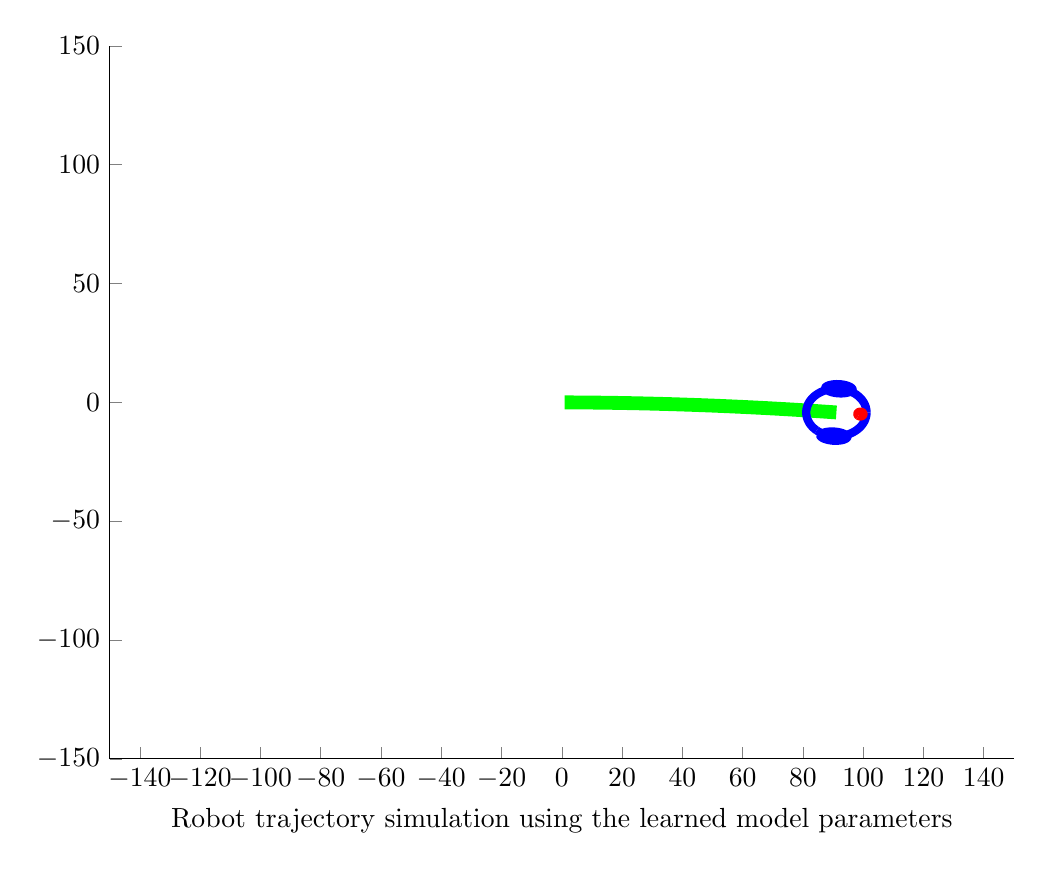
\begin{tikzpicture}

\begin{axis}[%
width=4.520833in,
height=3.565625in,
at={(0.758333in,0.48125in)},
scale only axis,
every outer x axis line/.append style={black},
every x tick label/.append style={font=\color{black}},
xmin=-150,
xmax=150,
xlabel={Robot trajectory simulation using the learned model parameters},
every outer y axis line/.append style={black},
every y tick label/.append style={font=\color{black}},
ymin=-150,
ymax=150,
axis x line*=bottom,
axis y line*=left
]
\addplot [color=green,solid,line width=5.0pt,forget plot]
  table[row sep=crcr]{%
0.912336607856475	-0.00388656348316623\\
1.82466956540827	-0.0085519654551722\\
2.73699820778096	-0.0139962025160459\\
3.64932187010326	-0.0202192706982294\\
4.56163988750751	-0.0272211654665812\\
5.47395159513017	-0.0350018817183801\\
6.3862563281123	-0.0435614137833286\\
7.29855342160004	-0.0528997554235571\\
8.2108422107451	-0.0630168998336285\\
9.12312203070523	-0.0739128396405432\\
10.0353922166447	-0.0855875669037442\\
10.9476521037349	-0.0980410731151233\\
11.8599010271546	-0.111273349199027\\
12.7721383220907	-0.125284385512263\\
13.6843633237383	-0.140074171844107\\
14.5965753673018	-0.155642697416313\\
15.5087737879948	-0.171989950883115\\
16.420957921041	-0.189115920331241\\
17.3331271016744	-0.20702059327992\\
18.2452806651399	-0.225703956680891\\
19.1574179466938	-0.245165996918411\\
20.0695382816043	-0.265406699809266\\
20.9816410051519	-0.286426050602783\\
21.89372545263	-0.308224033980839\\
22.8057909593453	-0.330800634057871\\
23.7178368606181	-0.35415583438089\\
24.6298624917834	-0.378289617929493\\
25.5418671881906	-0.403201967115873\\
26.4538502852045	-0.428892863784834\\
27.3658111182057	-0.455362289213803\\
28.2777490225909	-0.482610224112843\\
29.1896633337736	-0.510636648624672\\
30.1015533871845	-0.539441542324669\\
31.0134185182719	-0.569024884220896\\
31.9252580625023	-0.599386652754111\\
32.8370713553609	-0.630526825797782\\
33.7488577323519	-0.662445380658107\\
34.6606165289992	-0.695142294074026\\
35.572347080847	-0.72861754221724\\
36.4840487234596	-0.762871100692231\\
37.3957207924228	-0.797902944536275\\
38.3073626233438	-0.833713048219464\\
39.2189735518518	-0.870301385644721\\
40.1305529135986	-0.907667930147824\\
41.0421000442589	-0.945812654497419\\
41.953614279531	-0.984735530895047\\
42.8650949551371	-1.02443653097516\\
43.776541406824	-1.06491562580514\\
44.6879529703631	-1.10617278588532\\
45.5993289815516	-1.14820798114901\\
46.5106687762125	-1.19102118096253\\
47.421971690195	-1.23461235412521\\
48.3332370593755	-1.2789814688694\\
49.2444642196574	-1.32412849286054\\
50.1556525069723	-1.37005339319717\\
51.0668012572799	-1.41675613641091\\
51.9779098065688	-1.46423668846653\\
52.8889774908568	-1.51249501476197\\
53.8000036461916	-1.56153108012836\\
54.7109876086512	-1.61134484883002\\
55.6219287143441	-1.66193628456453\\
56.5328262994104	-1.71330535046273\\
57.4436797000215	-1.76545200908874\\
58.3544882523814	-1.81837622244001\\
59.2652512927266	-1.87207795194734\\
60.1759681573266	-1.92655715847491\\
61.0866381824848	-1.98181380232028\\
61.9972607045387	-2.03784784321446\\
62.9078350598604	-2.09465924032193\\
63.818360584857	-2.15224795224063\\
64.7288366159713	-2.21061393700206\\
65.6392624896821	-2.26975715207125\\
66.5496375425047	-2.32967755434681\\
67.4599611109917	-2.39037510016098\\
68.370232531733	-2.45184974527964\\
69.2804511413565	-2.51410144490235\\
70.1906162765285	-2.57713015366237\\
71.1007272739546	-2.64093582562672\\
72.0107834703796	-2.7055184142962\\
72.9207842025883	-2.7708778726054\\
73.8307288074058	-2.83701415292278\\
74.7406166216984	-2.90392720705067\\
75.6504469823734	-2.97161698622532\\
76.5602192263803	-3.04008344111692\\
77.4699326907108	-3.10932652182966\\
78.3795867123994	-3.17934617790175\\
79.2891806285241	-3.25014235830547\\
80.1987137762065	-3.32171501144717\\
81.1081854926125	-3.39406408516738\\
82.017595114953	-3.46718952674075\\
82.9269419804839	-3.5410912828762\\
83.8362254265069	-3.61576929971684\\
84.74544479037	-3.69122352284012\\
85.6545994094679	-3.7674538972578\\
86.5636886212422	-3.844460367416\\
87.4727117631826	-3.92224287719527\\
88.3816681728267	-4.00080136991059\\
89.2905571877608	-4.08013578831145\\
90.1993781456201	-4.16024607458187\\
91.1081303840898	-4.24113217034044\\
};
\addplot [color=blue,solid,line width=3.0pt,forget plot]
  table[row sep=crcr]{%
101.10813038409	-4.24113217034044\\
101.10812538409	-4.2311321720071\\
101.108110384097	-4.22113218367377\\
101.108085384124	-4.21113221534042\\
101.108050384197	-4.20113227700702\\
101.10800538435	-4.19113237867351\\
101.10795038463	-4.18113253033979\\
101.10788538509	-4.1711327420057\\
101.107810385797	-4.16113302367104\\
101.107725386824	-4.15113338533552\\
101.107630388257	-4.14113383699877\\
101.10752539019	-4.13113438866035\\
101.10741039273	-4.1211350503197\\
101.10728539599	-4.11113583197616\\
101.107150400096	-4.10113674362895\\
101.107005405183	-4.09113779527716\\
101.106850411396	-4.08113899691972\\
101.10668541889	-4.07114035855545\\
101.106510427829	-4.06114189018297\\
101.10632543839	-4.05114360180076\\
101.106130450756	-4.04114550340711\\
101.105925465122	-4.0311476050001\\
101.105710481695	-4.02114991657764\\
101.105485500688	-4.01115244813742\\
101.105250522327	-4.00115520967689\\
101.105005546847	-3.99115821119331\\
101.104750574492	-3.98116146268367\\
101.104485605518	-3.97116497414472\\
101.10421064019	-3.96116875557293\\
101.103925678782	-3.95117281696454\\
101.10363072158	-3.94117716831548\\
101.103325768878	-3.9311818196214\\
101.103010820982	-3.92118678087764\\
101.102685878206	-3.91119206207924\\
101.102350940875	-3.90119767322092\\
101.102006009325	-3.89120362429708\\
101.1016510839	-3.88120992530174\\
101.101286164955	-3.87121658622863\\
101.100911252855	-3.86122361707107\\
101.100526347975	-3.85123102782203\\
101.1001314507	-3.8412388284741\\
101.099726561424	-3.83124702901947\\
101.099311680554	-3.82125563944996\\
101.098886808502	-3.81126466975694\\
101.098451945696	-3.80127412993139\\
101.098007092568	-3.79128402996384\\
101.097552249565	-3.78129437984439\\
101.097087417141	-3.77130518956269\\
101.09661259576	-3.76131646910794\\
101.096127785898	-3.75132822846885\\
101.09563298804	-3.74134047763365\\
101.095128202679	-3.73135322659011\\
101.094613430322	-3.72136648532547\\
101.094088671482	-3.71138026382648\\
101.093553926685	-3.70139457207934\\
101.093009196466	-3.69140942006976\\
101.092454481368	-3.68142481778288\\
101.091889781947	-3.67144077520331\\
101.091315098768	-3.66145730231509\\
101.090730432404	-3.65147440910168\\
101.090135783442	-3.64149210554599\\
101.089531152475	-3.63151040163031\\
101.088916540108	-3.62152930733635\\
101.088291946955	-3.61154883264521\\
101.087657373642	-3.60156898753734\\
101.087012820803	-3.59158978199261\\
101.086358289082	-3.58161122599021\\
101.085693779134	-3.5716333295087\\
101.085019291623	-3.56165610252598\\
101.084334827225	-3.55167955501926\\
101.083640386623	-3.54170369696511\\
101.082935970511	-3.53172853833937\\
101.082221579595	-3.5217540891172\\
101.081497214589	-3.51178035927306\\
101.080762876216	-3.50180735878066\\
101.080018565212	-3.49183509761301\\
101.07926428232	-3.48186358574238\\
101.078500028296	-3.47189283314026\\
101.077725803902	-3.46192284977742\\
101.076941609914	-3.45195364562384\\
101.076147447116	-3.44198523064871\\
101.075343316301	-3.43201761482046\\
101.074529218275	-3.42205080810669\\
101.07370515385	-3.41208482047422\\
101.072871123851	-3.40211966188903\\
101.072027129113	-3.39215534231628\\
101.071173170478	-3.38219187172028\\
101.070309248802	-3.37222926006451\\
101.069435364947	-3.36226751731158\\
101.068551519789	-3.35230665342323\\
101.06765771421	-3.34234667836033\\
101.066753949104	-3.33238760208284\\
101.065840225376	-3.32242943454984\\
101.064916543939	-3.3124721857195\\
101.063982905717	-3.30251586554907\\
101.063039311642	-3.29256048399486\\
101.06208576266	-3.28260605101227\\
101.061122259723	-3.27265257655571\\
101.060148803795	-3.26270007057866\\
101.05916539585	-3.25274854303364\\
101.05817203687	-3.24279800387216\\
101.05716872785	-3.23284846304476\\
101.056155469792	-3.22289993050098\\
101.055132263709	-3.21295241618936\\
101.054099110626	-3.20300593005741\\
101.053056011575	-3.19306048205161\\
101.052002967599	-3.18311608211742\\
101.050939979751	-3.17317274019922\\
101.049867049095	-3.16323046624036\\
101.048784176702	-3.15328927018312\\
101.047691363657	-3.14334916196869\\
101.046588611051	-3.13341015153717\\
101.045475919988	-3.12347224882759\\
101.044353291581	-3.11353546377783\\
101.043220726951	-3.10359980632468\\
101.042078227232	-3.0936652864038\\
101.040925793566	-3.08373191394971\\
101.039763427105	-3.07379969889578\\
101.038591129012	-3.06386865117422\\
101.037408900459	-3.05393878071609\\
101.036216742629	-3.04401009745124\\
101.035014656712	-3.03408261130837\\
101.033802643913	-3.02415633221496\\
101.032580705442	-3.01423127009728\\
101.031348842521	-3.00430743488041\\
101.030107056383	-2.99438483648816\\
101.028855348269	-2.98446348484314\\
101.027593719431	-2.97454338986671\\
101.02632217113	-2.96462456147895\\
101.025040704639	-2.95470700959869\\
101.023749321238	-2.94479074414349\\
101.022448022219	-2.9348757750296\\
101.021136808883	-2.924962112172\\
101.019815682541	-2.91504976548435\\
101.018484644515	-2.905138744879\\
101.017143696135	-2.89522906026695\\
101.015792838743	-2.88532072155791\\
101.01443207369	-2.8754137386602\\
101.013061402335	-2.86550812148081\\
101.011680826051	-2.85560387992535\\
101.010290346216	-2.84570102389807\\
101.008889964223	-2.83579956330182\\
101.007479681471	-2.82589950803806\\
101.00605949937	-2.81600086800684\\
101.004629419341	-2.80610365310681\\
101.003189442814	-2.79620787323517\\
101.001739571228	-2.78631353828771\\
101.000279806035	-2.77642065815877\\
100.998810148692	-2.76652924274121\\
100.997330600671	-2.75663930192645\\
100.99584116345	-2.74675084560445\\
100.99434183852	-2.73686388366364\\
100.992832627378	-2.72697842599099\\
100.991313531536	-2.71709448247196\\
100.989784552511	-2.70721206299049\\
100.988245691832	-2.697331177429\\
100.986696951039	-2.68745183566838\\
100.985138331681	-2.67757404758796\\
100.983569835315	-2.66769782306553\\
100.981991463511	-2.65782317197732\\
100.980403217846	-2.64795010419798\\
100.978805099909	-2.63807862960057\\
100.977197111299	-2.62820875805656\\
100.975579253623	-2.61834049943584\\
100.973951528498	-2.60847386360665\\
100.972313937553	-2.59860886043563\\
100.970666482426	-2.58874549978778\\
100.969009164763	-2.57888379152647\\
100.967341986222	-2.56902374551339\\
100.965664948471	-2.55916537160861\\
100.963978053185	-2.54930867967048\\
100.962281302053	-2.5394536795557\\
100.960574696771	-2.52960038111927\\
100.958858239045	-2.51974879421448\\
100.957131930593	-2.50989892869293\\
100.955395773139	-2.50005079440448\\
100.953649768421	-2.49020440119725\\
100.951893918185	-2.48035975891765\\
100.950128224185	-2.47051687741032\\
100.948352688189	-2.46067576651813\\
100.946567311971	-2.4508364360822\\
100.944772097317	-2.44099889594185\\
100.942967046022	-2.43116315593462\\
100.941152159892	-2.42132922589626\\
100.93932744074	-2.41149711566069\\
100.937492890392	-2.40166683506003\\
100.935648510683	-2.39183839392454\\
100.933794303456	-2.38201180208268\\
100.931930270566	-2.37218706936103\\
100.930056413877	-2.36236420558433\\
100.928172735263	-2.35254322057543\\
100.926279236607	-2.34272412415533\\
100.924375919803	-2.33290692614311\\
100.922462786754	-2.32309163635598\\
100.920539839374	-2.31327826460923\\
100.918607079586	-2.30346682071622\\
100.916664509321	-2.2936573144884\\
100.914712130523	-2.28384975573527\\
100.912749945144	-2.27404415426439\\
100.910777955147	-2.26424051988136\\
100.908796162502	-2.25443886238982\\
100.906804569193	-2.24463919159143\\
100.90480317721	-2.23484151728584\\
100.902791988556	-2.22504584927074\\
100.90077100524	-2.2152521973418\\
100.898740229285	-2.20546057129266\\
100.896699662721	-2.19567098091495\\
100.894649307588	-2.18588343599825\\
100.892589165937	-2.17609794633012\\
100.890519239828	-2.16631452169604\\
100.888439531331	-2.15653317187944\\
100.886350042526	-2.14675390666166\\
100.884250775502	-2.13697673582198\\
100.882141732358	-2.12720166913755\\
100.880022915204	-2.11742871638344\\
100.877894326158	-2.10765788733261\\
100.875755967349	-2.09788919175589\\
100.873607840916	-2.08812263942197\\
100.871449949005	-2.0783582400974\\
100.869282293776	-2.06859600354658\\
100.867104877396	-2.05883593953174\\
100.864917702042	-2.04907805781296\\
100.862720769902	-2.0393223681481\\
100.860514083172	-2.02956888029286\\
100.858297644059	-2.01981760400073\\
100.856071454779	-2.01006854902298\\
100.85383551756	-2.00032172510867\\
100.851589834636	-1.99057714200461\\
100.849334408253	-1.9808348094554\\
100.847069240667	-1.97109473720335\\
100.844794334144	-1.96135693498855\\
100.842509690957	-1.9516214125488\\
100.840215313391	-1.94188817961961\\
100.837911203742	-1.93215724593422\\
100.835597364312	-1.92242862122357\\
100.833273797416	-1.91270231521627\\
100.830940505378	-1.90297833763863\\
100.82859749053	-1.89325669821463\\
100.826244755216	-1.88353740666591\\
100.823882301789	-1.87382047271175\\
100.82151013261	-1.86410590606909\\
100.819128250053	-1.8543937164525\\
100.816736656498	-1.84468391357417\\
100.814335354338	-1.83497650714389\\
100.811924345974	-1.82527150686907\\
100.809503633816	-1.81556892245472\\
100.807073220286	-1.80586876360341\\
100.804633107814	-1.7961710400153\\
100.802183298841	-1.78647576138813\\
100.799723795815	-1.77678293741715\\
100.797254601196	-1.76709257779521\\
100.794775717454	-1.75740469221265\\
100.792287147068	-1.74771929035736\\
100.789788892526	-1.73803638191474\\
100.787280956325	-1.72835597656771\\
100.784763340976	-1.71867808399666\\
100.782236048994	-1.70900271387948\\
100.779699082907	-1.69932987589155\\
100.777152445252	-1.6896595797057\\
100.774596138576	-1.67999183499223\\
100.772030165435	-1.67032665141889\\
100.769454528395	-1.66066403865084\\
100.766869230032	-1.65100400635072\\
100.76427427293	-1.64134656417854\\
100.761669659686	-1.63169172179175\\
100.759055392903	-1.62203948884519\\
100.756431475196	-1.6123898749911\\
100.753797909189	-1.60274288987908\\
100.751154697515	-1.59309854315612\\
100.748501842817	-1.58345684446657\\
100.745839347749	-1.57381780345213\\
100.743167214972	-1.56418142975182\\
100.74048544716	-1.55454773300204\\
100.737794046993	-1.54491672283647\\
100.735093017164	-1.53528840888612\\
100.732382360372	-1.52566280077931\\
100.72966207933	-1.51603990814164\\
100.726932176756	-1.50641974059601\\
100.724192655382	-1.49680230776257\\
100.721443517946	-1.48718761925878\\
100.718684767198	-1.4775756846993\\
100.715916405896	-1.46796651369608\\
100.713138436809	-1.45836011585828\\
100.710350862714	-1.44875650079231\\
100.7075536864	-1.43915567810177\\
100.704746910664	-1.4295576573875\\
100.701930538312	-1.4199624482475\\
100.69910457216	-1.41037006027699\\
100.696269015035	-1.40078050306835\\
100.693423869772	-1.39119378621114\\
100.690569139217	-1.38160991929208\\
100.687704826223	-1.37202891189503\\
100.684830933656	-1.36245077360101\\
100.681947464389	-1.35287551398814\\
100.679054421306	-1.34330314263168\\
100.6761518073	-1.33373366910401\\
100.673239625273	-1.3241671029746\\
100.670317878138	-1.31460345381001\\
100.667386568815	-1.3050427311739\\
100.664445700238	-1.29548494462698\\
100.661495275346	-1.28593010372704\\
100.65853529709	-1.27637821802892\\
100.65556576843	-1.26682929708451\\
100.652586692335	-1.25728335044272\\
100.649598071784	-1.24774038764951\\
100.646599909767	-1.23820041824782\\
100.643592209281	-1.22866345177764\\
100.640574973334	-1.21912949777593\\
100.637548204943	-1.20959856577663\\
100.634511907136	-1.20007066531069\\
100.631466082947	-1.190545805906\\
100.628410735424	-1.18102399708742\\
100.625345867621	-1.17150524837676\\
100.622271482603	-1.16198956929277\\
100.619187583445	-1.15247696935112\\
100.61609417323	-1.14296745806441\\
100.612991255053	-1.13346104494216\\
100.609878832015	-1.12395773949077\\
100.60675690723	-1.11445755121355\\
100.603625483819	-1.1049604896107\\
100.600484564914	-1.09546656417926\\
100.597334153656	-1.08597578441317\\
100.594174253194	-1.0764881598032\\
100.591004866689	-1.06700369983697\\
100.587825997311	-1.05752241399895\\
100.584637648238	-1.04804431177043\\
100.581439822658	-1.03856940262949\\
100.57823252377	-1.02909769605106\\
100.57501575478	-1.01962920150683\\
100.571789518906	-1.01016392846531\\
100.568553819374	-1.00070188639175\\
100.565308659419	-0.991243084748214\\
100.562054042286	-0.981787532993489\\
100.55878997123	-0.97233524058313\\
100.555516449516	-0.962886216969427\\
100.552233480416	-0.953440471601406\\
100.548941067214	-0.943998013924809\\
100.545639213202	-0.934558853382094\\
100.542327921683	-0.925122999412419\\
100.539007195966	-0.915690461451641\\
100.535677039373	-0.906261248932293\\
100.532337455235	-0.896835371283589\\
100.52898844689	-0.887412837931405\\
100.525630017688	-0.877993658298275\\
100.522262170987	-0.868577841803376\\
100.518884910155	-0.859165397862524\\
100.515498238569	-0.849756335888164\\
100.512102159617	-0.840350665289355\\
100.508696676693	-0.830948395471767\\
100.505281793204	-0.82154953583767\\
100.501857512564	-0.812154095785923\\
100.498423838197	-0.802762084711965\\
100.494980773539	-0.793373512007806\\
100.49152832203	-0.783988387062018\\
100.488066487124	-0.774606719259725\\
100.484595272283	-0.765228517982594\\
100.481114680978	-0.755853792608826\\
100.47762471669	-0.746482552513145\\
100.474125382907	-0.737114807066791\\
100.470616683131	-0.727750565637509\\
100.467098620869	-0.718389837589538\\
100.46357119964	-0.709032632283606\\
100.46003442297	-0.699678959076918\\
100.456488294398	-0.690328827323146\\
100.452932817468	-0.680982246372421\\
100.449367995737	-0.671639225571323\\
100.445793832768	-0.662299774262873\\
100.442210332137	-0.652963901786521\\
100.438617497427	-0.643631617478138\\
100.435015332231	-0.634302930670009\\
100.43140384015	-0.624977850690817\\
100.427783024797	-0.615656386865645\\
100.424152889792	-0.606338548515954\\
100.420513438765	-0.597024344959582\\
100.416864675356	-0.587713785510732\\
100.413206603213	-0.578406879479962\\
100.409539225995	-0.569103636174177\\
100.405862547369	-0.559804064896621\\
100.402176571011	-0.550508174946863\\
100.398481300608	-0.541215975620794\\
100.394776739855	-0.531927476210611\\
100.391062892456	-0.522642686004812\\
100.387339762126	-0.513361614288188\\
100.383607352587	-0.50408427034181\\
100.379865667571	-0.49481066344302\\
100.376114710822	-0.485540802865425\\
100.372354486088	-0.476274697878884\\
100.368584997132	-0.467012357749502\\
100.364806247721	-0.457753791739619\\
100.361018241636	-0.448499009107798\\
100.357220982663	-0.439248019108823\\
100.3534144746	-0.430000830993682\\
100.349598721255	-0.420757454009563\\
100.345773726441	-0.411517897399841\\
100.341939493985	-0.402282170404074\\
100.338096027721	-0.393050282257987\\
100.334243331492	-0.383822242193467\\
100.33038140915	-0.374598059438553\\
100.326510264559	-0.365377743217429\\
100.322629901588	-0.356161302750409\\
100.318740324119	-0.346948747253932\\
100.31484153604	-0.337740085940554\\
100.310933541251	-0.328535328018935\\
100.30701634366	-0.319334482693833\\
100.303089947183	-0.31013755916609\\
100.299154355748	-0.300944566632633\\
100.295209573289	-0.29175551428645\\
100.291255603752	-0.282570411316594\\
100.28729245109	-0.273389266908167\\
100.283320119268	-0.264212090242313\\
100.279338612256	-0.255038890496208\\
100.275347934037	-0.24586967684305\\
100.271348088601	-0.236704458452054\\
100.267339079948	-0.227543244488435\\
100.263320912087	-0.218386044113407\\
100.259293589036	-0.209232866484171\\
100.255257114823	-0.200083720753902\\
100.251211493484	-0.190938616071747\\
100.247156729065	-0.181797561582808\\
100.24309282562	-0.172660566428139\\
100.239019787213	-0.163527639744736\\
100.234937617918	-0.154398790665523\\
100.230846321816	-0.145274028319349\\
100.226745902999	-0.136153361830976\\
100.222636365567	-0.127036800321068\\
100.21851771363	-0.11792435290619\\
100.214389951307	-0.108816028698784\\
100.210253082724	-0.0997118368071757\\
100.20610711202	-0.0906117863355558\\
100.20195204334	-0.0815158863839738\\
100.197787880839	-0.0724241460483297\\
100.193614628681	-0.0633365744203616\\
100.189432291039	-0.0542531805876427\\
100.185240872097	-0.0451739736335632\\
100.181040376045	-0.0360989626373307\\
100.176830807083	-0.027028156673957\\
100.172612169422	-0.0179615648142448\\
100.16838446728	-0.00889919612478618\\
100.164147704884	0.000158940332051216\\
100.159901886472	0.0092128354981309\\
100.155647016289	0.0182624803195592\\
100.151383098591	0.0273078657466908\\
100.14711013764	0.0363489827341432\\
100.14282813771	0.0453858222407986\\
100.138537103084	0.0544183752298188\\
100.134237038051	0.0634466326686516\\
100.129927946913	0.0724705855290395\\
100.125609833977	0.0814902247870313\\
100.121282703563	0.0905055414229885\\
100.116946559998	0.0995165264215938\\
100.112601407617	0.108523170771865\\
100.108247250765	0.117525465467157\\
100.103884093798	0.126523401505177\\
100.099511941078	0.135516969887989\\
100.095130796976	0.144506161622026\\
100.090740665875	0.153490967718096\\
100.086341552165	0.162471379191393\\
100.081933460244	0.171447387061509\\
100.077516394521	0.180418982352434\\
100.073090359413	0.189386156092576\\
100.068655359345	0.198348899314761\\
100.064211398753	0.207307203056246\\
100.059758482081	0.216261058358727\\
100.055296613782	0.225210456268352\\
100.050825798317	0.234155387835722\\
100.046346040157	0.243095844115907\\
100.041857343783	0.252031816168452\\
100.037359713682	0.260963295057384\\
100.032853154352	0.269890271851225\\
100.028337670301	0.278812737623002\\
100.023813266043	0.287730683450246\\
100.019279946103	0.296644100415014\\
100.014737715014	0.305552979603889\\
100.010186577319	0.314457312107994\\
100.005626537568	0.323357089022995\\
100.001057600322	0.332252301449118\\
99.9964797701487	0.341142940491149\\
99.9918930516273	0.350028997258453\\
99.9872974493439	0.358910462864971\\
99.9826929678942	0.367787328429238\\
99.9780796118827	0.376659585074391\\
99.9734573859227	0.385527223928174\\
99.9688262946364	0.394390236122948\\
99.9641863426549	0.403248612795702\\
99.9595375346182	0.41210234508806\\
99.9548798751751	0.42095142414629\\
99.9502133689833	0.429795841121314\\
99.9455380207092	0.438635587168716\\
99.9408538350282	0.44747065344875\\
99.9361608166245	0.456301031126352\\
99.9314589701911	0.465126711371143\\
99.9267483004298	0.473947685357445\\
99.9220288120514	0.482763944264284\\
99.9173005097752	0.491575479275403\\
99.9125633983297	0.500382281579265\\
99.9078174824519	0.509184342369071\\
99.9030627668877	0.51798165284276\\
99.8982992563919	0.526774204203022\\
99.8935269557279	0.535561987657308\\
99.8887458696681	0.544344994417833\\
99.8839560029936	0.553123215701593\\
99.8791573604941	0.561896642730366\\
99.8743499469684	0.570665266730725\\
99.8695337672239	0.57942907893405\\
99.8647088260768	0.588188070576527\\
99.8598751283519	0.596942232899164\\
99.855032678883	0.605691557147803\\
99.8501814825125	0.614436034573117\\
99.8453215440917	0.623175656430631\\
99.8404528684804	0.631910413980723\\
99.8355754605474	0.640640298488638\\
99.83068932517	0.64936530122449\\
99.8257944672344	0.658085413463279\\
99.8208908916355	0.666800626484892\\
99.8159786032767	0.675510931574117\\
99.8110576070705	0.684216320020649\\
99.8061279079378	0.692916783119102\\
99.8011895108083	0.701612312169013\\
99.7962424206203	0.710302898474853\\
99.7912866423211	0.718988533346036\\
99.7863221808664	0.72766920809693\\
99.7813490412205	0.736344914046859\\
99.7763672283567	0.745015642520118\\
99.7713767472568	0.753681384845981\\
99.7663776029113	0.762342132358704\\
99.7613698003193	0.770997876397542\\
99.7563533444885	0.77964860830675\\
99.7513282404356	0.788294319435598\\
99.7462944931854	0.796935001138376\\
99.741252107772	0.805570644774401\\
99.7362010892375	0.814201241708032\\
99.731141442633	0.822826783308673\\
99.7260731730182	0.831447260950782\\
99.7209962854613	0.840062666013882\\
99.7159107850392	0.848672989882569\\
99.7108166768374	0.857278223946521\\
99.7057139659501	0.865878359600503\\
99.7006026574799	0.87447338824438\\
99.6954827565381	0.883063301283125\\
99.6903542682447	0.891648090126826\\
99.6852171977281	0.900227746190694\\
99.6800715501254	0.908802260895074\\
99.6749173305823	0.917371625665451\\
99.6697545442529	0.925935831932463\\
99.6645831963001	0.934494871131903\\
99.6594032918952	0.943048734704734\\
99.654214836218	0.95159741409709\\
99.6490178344572	0.960140900760294\\
99.6438122918096	0.968679186150863\\
99.6385982134808	0.977212261730506\\
99.6333756046849	0.985740118966155\\
99.6281444706445	0.994262749329949\\
99.6229048165907	1.00278014429926\\
99.6176566477632	1.01129229535669\\
99.6123999694101	1.0197991939901\\
99.6071347867882	1.02830083169258\\
99.6018611051625	1.03679719996249\\
99.5965789298069	1.04528829030348\\
99.5912882660034	1.05377409422444\\
99.5859891190427	1.06225460323959\\
99.580681494224	1.0707298088684\\
99.5753653968549	1.07919970263567\\
99.5700408322515	1.08766427607152\\
99.5647078057384	1.09612352071136\\
99.5593663226485	1.10457742809595\\
99.5540163883234	1.1130259897714\\
99.548658008113	1.12146919728912\\
99.5432911873757	1.12990704220593\\
99.5379159314782	1.13833951608398\\
99.532532245796	1.14676661049078\\
99.5271401357125	1.15518831699926\\
99.5217396066201	1.16360462718769\\
99.5163306639191	1.17201553263978\\
99.5109133130185	1.18042102494462\\
99.5054875593357	1.18882109569671\\
99.5000534082964	1.19721573649599\\
99.4946108653348	1.20560493894781\\
99.4891599358934	1.21398869466299\\
99.4837006254232	1.22236699525775\\
99.4782329393834	1.2307398323538\\
99.4727568832417	1.2391071975783\\
99.4672724624743	1.24746908256389\\
99.4617796825654	1.25582547894869\\
99.456278549008	1.26417637837629\\
99.4507690673031	1.27252177249581\\
99.4452512429602	1.28086165296184\\
99.4397250814972	1.28919601143451\\
99.4341905884401	1.29752483957946\\
99.4286477693235	1.30584812906785\\
99.4230966296903	1.31416587157642\\
99.4175371750915	1.3224780587874\\
99.4119694110866	1.33078468238862\\
99.4063933432433	1.33908573407345\\
99.4008089771378	1.34738120554084\\
99.3952163183544	1.35567108849532\\
99.3896153724858	1.363955374647\\
99.3840061451328	1.37223405571161\\
99.3783886419048	1.38050712341047\\
99.3727628684192	1.38877456947049\\
99.3671288303018	1.39703638562425\\
99.3614865331866	1.40529256360992\\
99.355835982716	1.41354309517132\\
99.3501771845405	1.42178797205793\\
99.3445101443189	1.43002718602487\\
99.3388348677181	1.43826072883293\\
99.3331513604137	1.44648859224856\\
99.3274596280888	1.45471076804391\\
99.3217596764355	1.46292724799678\\
99.3160515111535	1.47113802389072\\
99.3103351379511	1.47934308751494\\
99.3046105625446	1.48754243066438\\
99.2988777906587	1.49573604513969\\
99.293136828026	1.50392392274726\\
99.2873876803875	1.51210605529923\\
99.2816303534924	1.52028243461344\\
99.2758648530981	1.52845305251353\\
99.2700911849699	1.53661790082888\\
99.2643093548816	1.54477697139464\\
99.2585193686151	1.55293025605174\\
99.2527212319602	1.56107774664689\\
99.2469149507152	1.56921943503261\\
99.2411005306863	1.57735531306721\\
99.2352779776879	1.58548537261482\\
99.2294472975425	1.59360960554536\\
99.223608496081	1.60172800373462\\
99.217761579142	1.60984055906419\\
99.2119065525725	1.61794726342151\\
99.2060434222275	1.62604810869989\\
99.2001721939702	1.63414308679848\\
99.1942928736717	1.6422321896223\\
99.1884054672114	1.65031540908226\\
99.1825099804767	1.65839273709512\\
99.176606419363	1.66646416558357\\
99.170694789774	1.67452968647618\\
99.1647750976213	1.68258929170742\\
99.1588473488245	1.69064297321769\\
99.1529115493114	1.69869072295332\\
99.1469677050178	1.70673253286654\\
99.1410158218876	1.71476839491556\\
99.1350559058726	1.72279830106451\\
99.1290879629328	1.73082224328348\\
99.123111999036	1.73884021354854\\
99.1171280201583	1.74685220384172\\
99.1111360322837	1.75485820615101\\
99.105136041404	1.76285821247043\\
99.0991280535194	1.77085221479997\\
99.0931120746377	1.77884020514563\\
99.087088110775	1.78682217551941\\
99.0810561679553	1.79479811793935\\
99.0750162522105	1.8027680244295\\
99.0689683695804	1.81073188701996\\
99.062912526113	1.81868969774687\\
99.0568487278642	1.82664144865241\\
99.0507769808976	1.83458713178484\\
99.0446972912852	1.84252673919848\\
99.0386096651064	1.85046026295371\\
99.0325141084491	1.85838769511702\\
99.0264106274087	1.86630902776097\\
99.0202992280887	1.87422425296423\\
99.0141799166005	1.88213336281158\\
99.0080526990635	1.8900363493939\\
99.0019175816048	1.89793320480822\\
98.9957745703596	1.90582392115767\\
98.9896236714708	1.91370849055154\\
98.9834648910894	1.92158690510527\\
98.9772982353741	1.92945915694043\\
98.9711237104917	1.93732523818478\\
98.9649413226166	1.94518514097224\\
98.9587510779312	1.9530388574429\\
98.9525529826257	1.96088637974304\\
98.9463470428983	1.96872770002516\\
98.940133264955	1.97656281044792\\
98.9339116550093	1.98439170317622\\
98.9276822192831	1.99221437038117\\
98.9214449640057	2.00003080424009\\
98.9151998954143	2.00784099693656\\
98.9089470197541	2.01564494066039\\
98.9026863432779	2.02344262760762\\
98.8964178722464	2.03123404998058\\
98.890141612928	2.03901919998784\\
98.8838575715991	2.04679806984425\\
98.8775657545437	2.05457065177094\\
98.8712661680535	2.06233693799534\\
98.8649588184282	2.07009692075116\\
98.858643711975	2.07785059227841\\
98.8523208550092	2.08559794482343\\
98.8459902538536	2.09333897063885\\
98.8396519148388	2.10107366198367\\
98.833305844303	2.10880201112318\\
98.8269520485925	2.11652401032904\\
98.8205905340609	2.12423965187924\\
98.8142213070698	2.13194892805816\\
98.8078443739885	2.13965183115651\\
98.8014597411938	2.14734835347138\\
98.7950674150703	2.15503848730627\\
98.7886674020105	2.16272222497103\\
98.7822597084143	2.17039955878193\\
98.7758443406895	2.17807048106164\\
98.7694213052513	2.18573498413923\\
98.7629906085228	2.1933930603502\\
98.7565522569347	2.20104470203647\\
98.7501062569254	2.20868990154641\\
98.7436526149409	2.21632865123482\\
98.7371913374348	2.22396094346294\\
98.7307224308683	2.23158677059849\\
98.7242459017105	2.23920612501563\\
98.7177617564377	2.24681899909502\\
98.7112700015342	2.25442538522379\\
98.7047706434918	2.26202527579553\\
98.6982636888097	2.26961866321038\\
98.6917491439949	2.27720553987493\\
98.685227015562	2.28478589820231\\
98.6786973100331	2.29235973061218\\
98.672160033938	2.29992702953068\\
98.6656151938138	2.30748778739053\\
98.6590627962054	2.31504199663097\\
98.6525028476652	2.32258964969778\\
98.6459353547532	2.33013073904333\\
98.6393603240369	2.33766525712651\\
98.6327777620912	2.34519319641281\\
98.6261876754988	2.35271454937429\\
98.6195900708497	2.36022930848961\\
98.6129849547416	2.36773746624399\\
98.6063723337795	2.37523901512929\\
98.5997522145761	2.38273394764396\\
98.5931246037515	2.39022225629306\\
98.5864895079333	2.39770393358829\\
98.5798469337566	2.40517897204796\\
98.573196887864	2.41264736419705\\
98.5665393769054	2.42010910256715\\
98.5598744075386	2.42756417969654\\
98.5532019864283	2.43501258813014\\
98.546522120247	2.44245432041953\\
98.5398348156746	2.44988936912299\\
98.5331400793984	2.45731772680546\\
98.5264379181131	2.4647393860386\\
98.5197283385209	2.47215433940074\\
98.5130113473314	2.47956257947693\\
98.5062869512615	2.48696409885893\\
98.4995551570357	2.49435889014522\\
98.4928159713857	2.50174694594101\\
98.4860694010508	2.50912825885825\\
98.4793154527774	2.51650282151562\\
98.4725541333196	2.52387062653856\\
98.4657854494387	2.53123166655927\\
98.4590094079033	2.53858593421671\\
98.4522260154894	2.54593342215661\\
98.4454352789806	2.55327412303148\\
98.4386372051675	2.56060802950062\\
98.4318318008482	2.56793513423013\\
98.4250190728281	2.5752554298929\\
98.4181990279199	2.58256890916865\\
98.4113716729436	2.58987556474387\\
98.4045370147267	2.59717538931194\\
98.3976950601037	2.60446837557301\\
98.3908458159167	2.61175451623411\\
98.3839892890149	2.6190338040091\\
98.3771254862547	2.62630623161868\\
98.3702544145001	2.63357179179043\\
98.363376080622	2.64083047725879\\
98.3564904914989	2.64808228076508\\
98.3495976540163	2.65532719505749\\
98.3426975750669	2.66256521289111\\
98.335790261551	2.66979632702792\\
98.3288757203758	2.67702053023681\\
98.3219539584559	2.68423781529358\\
98.315024982713	2.69144817498093\\
98.3080888000761	2.69865160208852\\
98.3011454174814	2.70584808941292\\
98.2941948418723	2.71303762975764\\
98.2872370801993	2.72022021593313\\
98.2802721394202	2.72739584075682\\
98.2733000264999	2.73456449705308\\
98.2663207484106	2.74172617765325\\
98.2593343121316	2.74888087539566\\
98.2523407246492	2.7560285831256\\
98.245339992957	2.76316929369537\\
98.2383321240559	2.77030299996426\\
98.2313171249535	2.77742969479857\\
98.2242950026651	2.78454937107159\\
98.2172657642126	2.79166202166366\\
98.2102294166254	2.79876763946213\\
98.2031859669396	2.80586621736137\\
98.196135422199	2.81295774826281\\
98.1890777894538	2.82004222507492\\
98.1820130757618	2.82711964071322\\
98.1749412881878	2.8341899881003\\
98.1678624338034	2.84125326016581\\
98.1607765196876	2.84830944984649\\
98.1536835529262	2.85535855008613\\
98.1465835406122	2.86240055383564\\
98.1394764898457	2.86943545405302\\
98.1323624077336	2.87646324370337\\
98.1252413013901	2.8834839157589\\
98.1181131779363	2.89049746319893\\
98.1109780445002	2.89750387900993\\
98.1038359082171	2.90450315618547\\
98.0966867762291	2.91149528772628\\
98.0895306556852	2.91848026664023\\
98.0823675537416	2.92545808594234\\
98.0751974775615	2.93242873865479\\
98.0680204343148	2.93939221780693\\
98.0608364311787	2.94634851643528\\
98.0536454753371	2.95329762758354\\
98.046447573981	2.9602395443026\\
98.0392427343083	2.96717425965055\\
98.0320309635238	2.97410176669267\\
98.0248122688393	2.98102205850145\\
98.0175866574735	2.98793512815661\\
98.010354136652	2.99484096874506\\
98.0031147136073	3.00173957336099\\
97.9958683955789	3.00863093510577\\
97.988615189813	3.01551504708805\\
97.9813551035629	3.02239190242372\\
97.9740881440887	3.02926149423593\\
97.9668143186572	3.03612381565507\\
97.9595336345424	3.04297885981883\\
97.9522460990249	3.04982661987217\\
97.9449517193923	3.05666708896733\\
97.9376505029389	3.06350026026384\\
97.930342456966	3.07032612692852\\
97.9230275887815	3.07714468213552\\
97.9157059057004	3.08395591906627\\
97.9083774150444	3.09075983090955\\
97.9010421241419	3.09755641086143\\
97.8937000403282	3.10434565212535\\
97.8863511709455	3.11112754791205\\
97.8789955233425	3.11790209143965\\
97.8716331048749	3.1246692759336\\
97.8642639229052	3.13142909462672\\
97.8568879848025	3.13818154075919\\
97.8495052979428	3.14492660757856\\
97.8421158697087	3.15166428833977\\
97.8347197074897	3.15839457630514\\
97.8273168186819	3.16511746474437\\
97.8199072106883	3.17183294693459\\
97.8124908909184	3.17854101616031\\
97.8050678667885	3.18524166571346\\
97.7976381457217	3.1919348888934\\
97.7902017351477	3.19862067900689\\
97.7827586425029	3.20529902936816\\
97.7753088752304	3.21196993329884\\
97.76785244078	3.21863338412804\\
97.7603893466081	3.22528937519231\\
97.7529196001778	3.23193789983566\\
97.7454432089588	3.23857895140956\\
97.7379601804275	3.24521252327296\\
97.730470522067	3.25183860879229\\
97.7229742413669	3.25845720134147\\
97.7154713458235	3.2650682943019\\
97.7079618429397	3.27167188106249\\
97.700445740225	3.27826795501965\\
97.6929230451954	3.28485650957732\\
97.6853937653738	3.29143753814694\\
97.6778579082893	3.29801103414747\\
97.6703154814778	3.30457699100543\\
97.6627664924818	3.31113540215485\\
97.6552109488503	3.31768626103733\\
97.6476488581387	3.32422956110201\\
97.6400802279092	3.33076529580559\\
97.6325050657304	3.33729345861233\\
97.6249233791774	3.34381404299408\\
97.617335175832	3.35032704243024\\
97.6097404632824	3.35683245040783\\
97.6021392491232	3.36333026042143\\
97.5945315409557	3.36982046597323\\
97.5869173463875	3.37630306057302\\
97.579296673033	3.38277803773823\\
97.5716695285127	3.38924539099385\\
97.5640359204538	3.39570511387256\\
97.5563958564899	3.40215719991461\\
97.548749344261	3.40860164266794\\
97.5410963914138	3.41503843568808\\
97.533437005601	3.42146757253826\\
97.5257711944822	3.42788904678934\\
97.5180989657231	3.43430285201983\\
97.510420326996	3.44070898181595\\
97.5027352859794	3.44710742977155\\
97.4950438503585	3.45349818948819\\
97.4873460278246	3.45988125457512\\
97.4796418260757	3.46625661864926\\
97.4719312528158	3.47262427533525\\
97.4642143157556	3.47898421826544\\
97.4564910226119	3.48533644107989\\
97.4487613811082	3.49168093742636\\
97.441025398974	3.49801770096038\\
97.4332830839453	3.50434672534517\\
97.4255344437644	3.51066800425171\\
97.4177794861801	3.51698153135872\\
97.4100182189471	3.52328730035267\\
97.4022506498268	3.5295853049278\\
97.3944767865868	3.5358755387861\\
97.3866966370009	3.54215799563735\\
97.3789102088493	3.54843266919907\\
97.3711175099183	3.55469955319661\\
97.3633185480008	3.56095864136307\\
97.3555133308956	3.56720992743937\\
97.347701866408	3.57345340517422\\
97.3398841623495	3.57968906832414\\
97.3320602265376	3.58591691065348\\
97.3242300667965	3.5921369259344\\
97.3163936909562	3.59834910794687\\
97.3085511068531	3.60455345047871\\
97.3007023223298	3.61074994732559\\
97.292847345235	3.616938592291\\
97.2849861834239	3.6231193791863\\
97.2771188447574	3.62929230183071\\
97.269245337103	3.63545735405131\\
97.2613656683342	3.64161452968304\\
97.2534798463305	3.64776382256872\\
97.245587878978	3.65390522655907\\
97.2376897741684	3.66003873551268\\
97.2297855398	3.66616434329604\\
97.2218751837769	3.67228204378354\\
97.2139587140095	3.6783918308575\\
97.2060361384143	3.68449369840811\\
97.1981074649139	3.69058764033351\\
97.1901727014369	3.69667365053976\\
97.1822318559181	3.70275172294086\\
97.1742849362983	3.70882185145872\\
97.1663319505245	3.71488403002322\\
97.1583729065496	3.72093825257219\\
97.1504078123327	3.7269845130514\\
97.1424366758388	3.73302280541458\\
97.1344595050392	3.73905312362346\\
97.126476307911	3.7450754616477\\
97.1184870924373	3.75108981346498\\
97.1104918666074	3.75709617306095\\
97.1024906384166	3.76309453442923\\
97.094483415866	3.76908489157148\\
97.0864702069628	3.77506723849733\\
97.0784510197204	3.78104156922445\\
97.0704258621578	3.78700787777849\\
97.0623947423002	3.79296615819315\\
97.0543576681787	3.79891640451016\\
97.0463146478305	3.80485861077925\\
97.0382656892985	3.81079277105824\\
97.0302108006317	3.81671887941296\\
97.0221499898849	3.8226369299173\\
97.0140832651191	3.82854691665321\\
97.0060106344008	3.83444883371071\\
96.9979321058028	3.84034267518787\\
96.9898476874036	3.84622843519086\\
96.9817573872876	3.85210610783393\\
96.973661213545	3.85797568723938\\
96.9655591742721	3.86383716753766\\
96.9574512775709	3.86969054286727\\
96.9493375315493	3.87553580737485\\
96.941217944321	3.88137295521512\\
96.9330925240057	3.88720198055095\\
96.9249612787287	3.8930228775533\\
96.9168242166213	3.89883564040128\\
96.9086813458205	3.90464026328213\\
96.9005326744693	3.91043674039123\\
96.8923782107162	3.91622506593209\\
96.8842179627159	3.9220052341164\\
96.8760519386284	3.92777723916398\\
96.8678801466198	3.93354107530283\\
96.859702594862	3.93929673676912\\
96.8515192915324	3.94504421780719\\
96.8433302448144	3.95078351266955\\
96.835135462897	3.9565146156169\\
96.826934953975	3.96223752091816\\
96.818728726249	3.96795222285041\\
96.810516787925	3.97365871569894\\
96.8022991472152	3.97935699375728\\
96.794075812337	3.98504705132714\\
96.7858467915139	3.99072888271846\\
96.7776120929748	3.99640248224941\\
96.7693717249545	4.0020678442464\\
96.7611256956934	4.00772496304406\\
96.7528740134374	4.01337383298528\\
96.7446166864382	4.01901444842118\\
96.7363537229533	4.02464680371115\\
96.7280851312454	4.03027089322283\\
96.7198109195833	4.03588671133214\\
96.7115310962411	4.04149425242326\\
96.7032456694986	4.04709351088864\\
96.6949546476413	4.05268448112903\\
96.6866580389603	4.05826715755347\\
96.678355851752	4.06384153457927\\
96.6700480943188	4.06940760663205\\
96.6617347749683	4.07496536814575\\
96.6534159020138	4.08051481356261\\
96.6450914837743	4.08605593733317\\
96.6367615285742	4.09158873391632\\
96.6284260447434	4.09711319777926\\
96.6200850406174	4.10262932339753\\
96.6117385245372	4.108137105255\\
96.6033865048493	4.11363653784389\\
96.5950289899057	4.11912761566477\\
96.586665988064	4.12461033322656\\
96.5782975076872	4.13008468504654\\
96.5699235571437	4.13555066565036\\
96.5615441448074	4.14100826957205\\
96.5531592790579	4.14645749135399\\
96.5447689682799	4.15189832554697\\
96.5363732208638	4.15733076671016\\
96.5279720452053	4.16275480941111\\
96.5195654497056	4.16817044822578\\
96.5111534427712	4.17357767773853\\
96.5027360328143	4.17897649254213\\
96.4943132282522	4.18436688723777\\
96.4858850375077	4.18974885643506\\
96.4774514690089	4.19512239475202\\
96.4690125311895	4.20048749681513\\
96.4605682324885	4.20584415725927\\
96.45211858135	4.21119237072778\\
96.4436635862238	4.21653213187246\\
96.4352032555648	4.22186343535354\\
96.4267375978334	4.22718627583972\\
96.4182666214952	4.23250064800815\\
96.4097903350212	4.23780654654448\\
96.4013087468878	4.2431039661428\\
96.3928218655764	4.24839290150568\\
96.3843296995739	4.25367334734421\\
96.3758322573726	4.25894529837792\\
96.3673295474698	4.26420874933487\\
96.3588215783683	4.26946369495161\\
96.3503083585761	4.2747101299732\\
96.3417898966063	4.27994804915319\\
96.3332662009775	4.28517744725368\\
96.3247372802133	4.29039831904526\\
96.3162031428426	4.29561065930706\\
96.3076637973995	4.30081446282674\\
96.2991192524236	4.3060097244005\\
96.2905695164591	4.31119643883307\\
96.282014598056	4.31637460093776\\
96.2734545057691	4.32154420553638\\
96.2648892481584	4.32670524745934\\
96.2563188337894	4.3318577215456\\
96.2477432712323	4.33700162264268\\
96.2391625690628	4.34213694560668\\
96.2305767358615	4.34726368530228\\
96.2219857802143	4.35238183660274\\
96.2133897107122	4.35749139438991\\
96.2047885359511	4.36259235355423\\
96.1961822645323	4.36768470899474\\
96.187570905062	4.3727684556191\\
96.1789544661517	4.37784358834354\\
96.1703329564176	4.38291010209295\\
96.1617063844815	4.3879679918008\\
96.1530747589697	4.39301725240921\\
96.144438088514	4.39805787886891\\
96.135796381751	4.40308986613928\\
96.1271496473225	4.40811320918834\\
96.118497893875	4.41312790299274\\
96.1098411300605	4.41813394253779\\
96.1011793645357	4.42313132281745\\
96.0925126059623	4.42812003883433\\
96.0838408630071	4.43310008559973\\
96.0751641443419	4.4380714581336\\
96.0664824586432	4.44303415146456\\
96.057795814593	4.44798816062992\\
96.0491042208777	4.45293348067568\\
96.040407686189	4.45787010665651\\
96.0317062192233	4.46279803363578\\
96.0229998286823	4.46771725668558\\
96.0142885232722	4.47262777088668\\
96.0055723117044	4.47752957132856\\
95.9968512026951	4.48242265310943\\
95.9881252049654	4.4873070113362\\
95.9793943272413	4.49218264112451\\
95.9706585782536	4.49704953759874\\
95.9619179667381	4.501907695892\\
95.9531725014354	4.50675711114611\\
95.9444221910911	4.51159777851167\\
95.9356670444553	4.51642969314802\\
95.9269070702833	4.52125285022323\\
95.918142277335	4.52606724491415\\
95.9093726743752	4.53087287240638\\
95.9005982701735	4.5356697278943\\
95.8918190735043	4.54045780658106\\
95.8830350931468	4.54523710367857\\
95.8742463378851	4.55000761440754\\
95.8654528165077	4.55476933399745\\
95.8566545378084	4.5595222576866\\
95.8478515105852	4.56426638072205\\
95.8390437436414	4.56900169835968\\
95.8302312457845	4.57372820586418\\
95.8214140258273	4.57844589850904\\
95.8125920925867	4.58315477157656\\
95.8037654548848	4.58785482035788\\
95.7949341215483	4.59254604015294\\
95.7860981014084	4.59722842627053\\
95.7772574033012	4.60190197402825\\
95.7684120360674	4.60656667875257\\
95.7595620085523	4.61122253577878\\
95.7507073296059	4.61586954045102\\
95.741848008083	4.62050768812229\\
95.7329840528429	4.62513697415443\\
95.7241154727494	4.62975739391818\\
95.7152422766713	4.63436894279309\\
95.7063644734817	4.63897161616764\\
95.6974820720583	4.64356540943913\\
95.6885950812837	4.64815031801379\\
95.6797035100447	4.6527263373067\\
95.670807367233	4.65729346274184\\
95.6619066617447	4.66185168975209\\
95.6530014024805	4.66640101377923\\
95.6440915983456	4.67094143027392\\
95.6351772582499	4.67547293469575\\
95.6262583911078	4.67999552251322\\
95.6173350058379	4.68450918920374\\
95.6084071113639	4.68901393025365\\
95.5994747166135	4.6935097411582\\
95.5905378305191	4.69799661742158\\
95.5815964620176	4.70247455455692\\
95.5726506200505	4.70694354808628\\
95.5637003135635	4.71140359354067\\
95.5547455515069	4.71585468646004\\
95.5457863428356	4.7202968223933\\
95.5368226965086	4.72472999689831\\
95.5278546214897	4.7291542055419\\
95.5188821267469	4.73356944389987\\
95.5099052212528	4.73797570755697\\
95.5009239139842	4.74237299210694\\
95.4919382139224	4.74676129315249\\
95.4829481300531	4.75114060630533\\
95.4739536713665	4.75551092718615\\
95.464954846857	4.75987225142461\\
95.4559516655233	4.76422457465941\\
95.4469441363688	4.76856789253821\\
95.4379322684008	4.77290220071769\\
95.4289160706313	4.77722749486356\\
95.4198955520765	4.78154377065052\\
95.4108707217569	4.78585102376228\\
95.4018415886973	4.7901492498916\\
95.3928081619269	4.79443844474026\\
95.383770450479	4.79871860401905\\
95.3747284633914	4.80298972344782\\
95.3656822097061	4.80725179875545\\
95.3566316984694	4.81150482567987\\
95.3475769387316	4.81574879996805\\
95.3385179395477	4.81998371737601\\
95.3294547099766	4.82420957366883\\
95.3203872590815	4.82842636462067\\
95.3113155959298	4.83263408601473\\
95.3022397295933	4.83683273364329\\
95.2931596691479	4.8410223033077\\
95.2840754236734	4.8452027908184\\
95.2749870022543	4.84937419199489\\
95.2658944139789	4.85353650266577\\
95.2567976679399	4.85768971866874\\
95.2476967732338	4.86183383585058\\
95.2385917389618	4.86596885006718\\
95.2294825742287	4.87009475718351\\
95.2203692881438	4.87421155307367\\
95.2112518898203	4.87831923362087\\
95.2021303883757	4.88241779471742\\
95.1930047929314	4.88650723226477\\
95.1838751126131	4.89058754217348\\
95.1747413565503	4.89465872036324\\
95.1656035338769	4.89872076276287\\
95.1564616537307	4.90277366531032\\
95.1473157252536	4.9068174239527\\
95.1381657575914	4.91085203464625\\
95.1290117598943	4.91487749335636\\
95.119853741316	4.91889379605757\\
95.1106917110148	4.92290093873357\\
95.1015256781526	4.92689891737723\\
95.0923556518954	4.93088772799057\\
95.0831816414133	4.93486736658477\\
95.0740036558802	4.9388378291802\\
95.0648217044742	4.94279911180639\\
95.0556357963772	4.94675121050207\\
95.0464459407751	4.95069412131513\\
95.0372521468579	4.95462784030267\\
95.0280544238191	4.95855236353096\\
95.0188527808567	4.96246768707548\\
95.0096472271722	4.96637380702092\\
95.0004377719711	4.97027071946114\\
94.991224424463	4.97415842049925\\
94.9820071938612	4.97803690624753\\
94.9727860893829	4.98190617282749\\
94.9635611202492	4.98576621636989\\
94.9543322956851	4.98961703301467\\
94.9450996249194	4.99345861891102\\
94.9358631171848	4.99729097021734\\
94.9266227817178	5.0011140831013\\
94.9173786277587	5.00492795373977\\
94.9081306645516	5.00873257831888\\
94.8988789013446	5.01252795303402\\
94.8896233473894	5.01631407408981\\
94.8803640119416	5.02009093770012\\
94.8711009042604	5.0238585400881\\
94.8618340336091	5.02761687748614\\
94.8525634092544	5.03136594613591\\
94.8432890404669	5.03510574228833\\
94.8340109365212	5.03883626220361\\
94.8247291066952	5.04255750215123\\
94.8154435602708	5.04626945840995\\
94.8061543065335	5.04997212726782\\
94.7968613547726	5.05366550502217\\
94.787564714281	5.05734958797961\\
94.7782643943554	5.06102437245607\\
94.7689604042961	5.06468985477676\\
94.7596527534071	5.06834603127621\\
94.7503414509961	5.07199289829822\\
94.7410265063742	5.07563045219595\\
94.7317079288566	5.07925868933182\\
94.7223857277617	5.08287760607762\\
94.7130599124118	5.08648719881442\\
94.7037304921326	5.09008746393262\\
94.6943974762536	5.09367839783197\\
94.6850608741078	5.09725999692153\\
94.6757206950319	5.1008322576197\\
94.6663769483659	5.10439517635422\\
94.6570296434537	5.10794874956217\\
94.6476787896425	5.11149297368998\\
94.6383243962832	5.11502784519342\\
94.6289664727301	5.11855336053763\\
94.6196050283413	5.12206951619709\\
94.6102400724781	5.12557630865564\\
94.6008716145055	5.1290737344065\\
94.591499663792	5.13256178995223\\
94.5821242297095	5.13604047180478\\
94.5727453216334	5.13950977648547\\
94.5633629489427	5.14296970052499\\
94.5539771210198	5.14642024046343\\
94.5445878472503	5.14986139285024\\
94.5351951370237	5.15329315424427\\
94.5257989997326	5.15671552121375\\
94.5163994447732	5.16012849033633\\
94.506996481545	5.16353205819903\\
94.497590119451	5.16692622139828\\
94.4881803678976	5.17031097653993\\
94.4787672362944	5.17368632023921\\
94.4693507340547	5.17705224912079\\
94.4599308705949	5.18040875981874\\
94.4505076553349	5.18375584897654\\
94.4410810976979	5.1870935132471\\
94.4316512071104	5.19042174929277\\
94.4222179930025	5.1937405537853\\
94.4127814648071	5.1970499234059\\
94.403341631961	5.20034985484519\\
94.3938985039039	5.20364034480324\\
94.384452090079	5.20692138998956\\
94.3750023999326	5.21019298712311\\
94.3655494429145	5.21345513293229\\
94.3560932284776	5.21670782415495\\
94.3466337660781	5.21995105753841\\
94.3371710651755	5.22318482983943\\
94.3277051352325	5.22640913782423\\
94.3182359857151	5.22962397826852\\
94.3087636260922	5.23282934795745\\
94.2992880658365	5.23602524368565\\
94.2898093144233	5.23921166225722\\
94.2803273813314	5.24238860048576\\
94.2708422760428	5.24555605519431\\
94.2613540080425	5.24871402321543\\
94.2518625868189	5.25186250139114\\
94.2423680218634	5.25500148657297\\
94.2328703226705	5.25813097562194\\
94.2233694987379	5.26125096540855\\
94.2138655595665	5.26436145281282\\
94.2043585146601	5.26746243472426\\
94.1948483735259	5.27055390804189\\
94.1853351456739	5.27363586967423\\
94.1758188406174	5.27670831653932\\
94.1662994678727	5.27977124556472\\
94.1567770369592	5.2828246536875\\
94.1472515573993	5.28586853785424\\
94.1377230387185	5.28890289502108\\
94.1281914904453	5.29192772215364\\
94.1186569221112	5.2949430162271\\
94.1091193432509	5.29794877422617\\
94.0995787634018	5.30094499314509\\
94.0900351921046	5.30393166998765\\
94.0804886389028	5.30690880176715\\
94.070939113343	5.30987638550649\\
94.0613866249748	5.31283441823806\\
94.0518311833505	5.31578289700384\\
94.0422727980257	5.31872181885534\\
94.0327114785588	5.32165118085366\\
94.0231472345109	5.32457098006942\\
94.0135800754465	5.32748121358283\\
94.0040100109326	5.33038187848365\\
93.9944370505394	5.33327297187122\\
93.9848612038397	5.33615449085445\\
93.9752824804094	5.33902643255181\\
93.9657008898273	5.34188879409137\\
93.9561164416749	5.34474157261076\\
93.9465291455367	5.34758476525721\\
93.9369390109999	5.35041836918752\\
93.9273460476548	5.3532423815681\\
93.9177502650942	5.35605679957492\\
93.908151672914	5.35886162039357\\
93.8985502807128	5.36165684121922\\
93.8889460980918	5.36444245925667\\
93.8793391346554	5.36721847172029\\
93.8697294000105	5.36998487583407\\
93.8601169037668	5.3727416688316\\
93.8505016555368	5.37548884795609\\
93.8408836649357	5.37822641046037\\
93.8312629415816	5.38095435360687\\
93.8216394950952	5.38367267466764\\
93.8120133350999	5.38638137092437\\
93.8023844712218	5.38908043966837\\
93.7927529130899	5.39176987820055\\
93.7831186703357	5.39444968383149\\
93.7734817525935	5.39711985388138\\
93.7638421695	5.39978038568005\\
93.7541999306951	5.40243127656696\\
93.7445550458207	5.40507252389124\\
93.734907524522	5.40770412501162\\
93.7252573764463	5.41032607729651\\
93.7156046112439	5.41293837812396\\
93.7059492385674	5.41554102488166\\
93.6962912680723	5.41813401496697\\
93.6866307094165	5.4207173457869\\
93.6769675722607	5.42329101475812\\
93.6673018662678	5.42585501930697\\
93.6576336011037	5.42840935686942\\
93.6479627864366	5.43095402489116\\
93.6382894319373	5.4334890208275\\
93.6286135472791	5.43601434214347\\
93.618935142138	5.43852998631372\\
93.6092542261924	5.44103595082263\\
93.5995708091231	5.44353223316422\\
93.5898849006136	5.44601883084222\\
93.5801965103498	5.44849574137002\\
93.57050564802	5.45096296227071\\
93.5608123233152	5.45342049107709\\
93.5511165459287	5.4558683253316\\
93.5414183255562	5.45830646258643\\
93.531717671896	5.46073490040344\\
93.5220145946487	5.46315363635418\\
93.5123091035174	5.46556266801993\\
93.5026012082075	5.46796199299165\\
93.4928909184271	5.47035160887001\\
93.4831782438863	5.4727315132654\\
93.4734631942978	5.47510170379792\\
93.4637457793768	5.47746217809737\\
93.4540260088405	5.47981293380329\\
93.4443038924088	5.48215396856491\\
93.4345794398038	5.4844852800412\\
93.4248526607499	5.48680686590085\\
93.4151235649739	5.48911872382228\\
93.405392162205	5.49142085149362\\
93.3956584621744	5.49371324661276\\
93.385922474616	5.49599590688728\\
93.3761842092657	5.49826883003455\\
93.3664436758617	5.50053201378162\\
93.3567008841447	5.50278545586532\\
93.3469558438573	5.5050291540322\\
93.3372085647446	5.50726310603858\\
93.327459056554	5.50948730965049\\
93.3177073290349	5.51170176264373\\
93.307953391939	5.51390646280385\\
93.2981972550203	5.51610140792615\\
93.2884389280349	5.51828659581569\\
93.2786784207411	5.52046202428727\\
93.2689157428995	5.52262769116548\\
93.2591509042727	5.52478359428463\\
93.2493839146255	5.52692973148883\\
93.239614783725	5.52906610063195\\
93.2298435213403	5.53119269957761\\
93.2200701372426	5.53330952619921\\
93.2102946412054	5.53541657837994\\
93.200517043004	5.53751385401273\\
93.1907373524162	5.5396013510003\\
93.1809555792216	5.54167906725518\\
93.171171733202	5.54374700069963\\
93.1613858241411	5.54580514926572\\
93.1515978618251	5.54785351089531\\
93.1418078560417	5.54989208354004\\
93.132015816581	5.55192086516132\\
93.122221753235	5.55393985373039\\
93.1124256757979	5.55594904722825\\
93.1026275940656	5.5579484436457\\
93.0928275178363	5.55993804098337\\
93.08302545691	5.56191783725163\\
93.0732214210887	5.56388783047071\\
93.0634154201767	5.5658480186706\\
93.0536074639797	5.56779839989112\\
93.0437975623059	5.56973897218189\\
93.033985724965	5.57166973360233\\
93.0241719617689	5.57359068222169\\
93.0143562825314	5.57550181611901\\
93.0045386970682	5.57740313338316\\
92.9947192151968	5.57929463211283\\
92.9848978467368	5.58117631041651\\
92.9750746015094	5.58304816641253\\
92.965249489338	5.58491019822904\\
92.9554225200476	5.58676240400399\\
92.9455937034652	5.58860478188519\\
92.9357630494197	5.59043733003025\\
92.9259305677417	5.59226004660664\\
92.9160962682636	5.59407292979162\\
92.9062601608198	5.59587597777233\\
92.8964222552464	5.59766918874571\\
92.8865825613813	5.59945256091854\\
92.8767410890641	5.60122609250747\\
92.8668978481364	5.60298978173896\\
92.8570528484413	5.60474362684931\\
92.8472060998239	5.60648762608468\\
92.837357612131	5.60822177770108\\
92.827507395211	5.60994607996436\\
92.8176554589141	5.6116605311502\\
92.8078018130923	5.61336512954417\\
92.7979464675991	5.61505987344165\\
92.7880894322901	5.61674476114791\\
92.7782307170221	5.61841979097806\\
92.768370331654	5.62008496125708\\
92.758508286046	5.62174027031978\\
92.7486445900603	5.62338571651086\\
92.7387792535605	5.62502129818488\\
92.7289122864119	5.62664701370625\\
92.7190436984816	5.62826286144927\\
92.7091734996382	5.62986883979807\\
92.6993016997517	5.63146494714668\\
92.689428308694	5.633051181899\\
92.6795533363386	5.63462754246879\\
92.6696767925604	5.63619402727969\\
92.6597986872358	5.63775063476522\\
92.6499190302431	5.63929736336876\\
92.6400378314619	5.64083421154359\\
92.6301551007733	5.64236117775287\\
92.6202708480602	5.64387826046962\\
92.6103850832067	5.64538545817676\\
92.6004978160987	5.6468827693671\\
92.5906090566233	5.64837019254332\\
92.5807188146694	5.64984772621801\\
92.5708271001272	5.65131536891362\\
92.5609339228884	5.65277311916252\\
92.5510392928461	5.65422097550695\\
92.5411432198951	5.65565893649906\\
92.5312457139314	5.65708700070089\\
92.5213467848524	5.65850516668437\\
92.5114464425572	5.65991343303134\\
92.501544696946	5.66131179833353\\
92.4916415579207	5.66270026119258\\
92.4817370353843	5.66407882022002\\
92.4718311392413	5.6654474740373\\
92.4619238793977	5.66680622127576\\
92.4520152657607	5.66815506057665\\
92.442105308239	5.66949399059114\\
92.4321940167424	5.67082300998029\\
92.4222814011823	5.67214211741509\\
92.4123674714713	5.67345131157643\\
92.4024522375233	5.67475059115511\\
92.3925357092536	5.67603995485185\\
92.3826178965787	5.6773194013773\\
92.3726988094163	5.678588929452\\
92.3627784576857	5.67984853780643\\
92.352856851307	5.68109822518098\\
92.342934000202	5.68233799032596\\
92.3330099142935	5.6835678320016\\
92.3230846035056	5.68478774897807\\
92.3131580777635	5.68599774003545\\
92.3032303469939	5.68719780396374\\
92.2933014211244	5.68838793956289\\
92.2833713100839	5.68956814564275\\
92.2734400238026	5.69073842102313\\
92.2635075722118	5.69189876453374\\
92.2535739652439	5.69304917501425\\
92.2436392128325	5.69418965131424\\
92.2337033249123	5.69532019229323\\
92.2237663114194	5.69644079682069\\
92.2138281822905	5.69755146377601\\
92.203888947464	5.69865219204853\\
92.193948616879	5.69974298053751\\
92.1840072004759	5.70082382815217\\
92.174064708196	5.70189473381165\\
92.1641211499819	5.70295569644507\\
92.1541765357772	5.70400671499144\\
92.1442308755263	5.70504778839976\\
92.1342841791751	5.70607891562895\\
92.1243364566701	5.70710009564788\\
92.1143877179592	5.70811132743537\\
92.104437972991	5.7091126099802\\
92.0944872317153	5.71010394228107\\
92.0845355040828	5.71108532334666\\
92.0745828000453	5.71205675219559\\
92.0646291295555	5.71301822785642\\
92.054674502567	5.71396974936769\\
92.0447189290344	5.71491131577786\\
92.0347624189134	5.71584292614538\\
92.0248049821604	5.71676457953863\\
92.0148466287329	5.71767627503596\\
92.0048873685893	5.71857801172568\\
91.9949272116887	5.71946978870604\\
91.9849661679914	5.72035160508528\\
91.9750042474584	5.72122345998157\\
91.9650414600515	5.72208535252306\\
91.9550778157337	5.72293728184785\\
91.9451133244685	5.72377924710403\\
91.9351479962205	5.72461124744962\\
91.9251818409548	5.72543328205262\\
91.9152148686378	5.726245350091\\
91.9052470892364	5.72704745075269\\
91.8952785127184	5.72783958323558\\
91.8853091490523	5.72862174674756\\
91.8753390082075	5.72939394050645\\
91.8653681001541	5.73015616374006\\
91.8553964348631	5.73090841568617\\
91.845424022306	5.73165069559252\\
91.8354508724555	5.73238300271683\\
91.8254769952844	5.73310533632681\\
91.8155024007669	5.73381769570011\\
91.8055270988773	5.73452008012437\\
91.7955510995912	5.73521248889722\\
91.7855744128843	5.73589492132623\\
91.7755970487335	5.73656737672899\\
91.7656190171161	5.73722985443303\\
91.7556403280101	5.73788235377588\\
91.7456609913942	5.73852487410504\\
91.7356810172477	5.73915741477798\\
91.7257004155507	5.73977997516217\\
91.7157191962837	5.74039255463504\\
91.7057373694279	5.74099515258403\\
91.6957549449652	5.74158776840652\\
91.685771932878	5.7421704015099\\
91.6757883431493	5.74274305131155\\
91.6658041857627	5.7433057172388\\
91.6558194707023	5.743858398729\\
91.6458342079529	5.74440109522947\\
91.6358484074997	5.74493380619749\\
91.6258620793285	5.74545653110038\\
91.6158752334256	5.74596926941539\\
91.605887879778	5.7464720206298\\
91.5959000283729	5.74696478424085\\
91.5859116891982	5.74744755975578\\
91.5759228722422	5.74792034669181\\
91.5659335874938	5.74838314457615\\
91.5559438449422	5.74883595294601\\
91.5459536545772	5.74927877134859\\
91.535963026389	5.74971159934105\\
91.5259719703681	5.75013443649057\\
91.5159804965058	5.75054728237432\\
91.5059886147933	5.75095013657945\\
91.4959963352226	5.75134299870311\\
91.486003667786	5.75172586835243\\
91.4760106224762	5.75209874514455\\
91.4660172092861	5.75246162870658\\
91.4560234382093	5.75281451867564\\
91.4460293192394	5.75315741469885\\
91.4360348623706	5.75349031643331\\
91.4260400775974	5.75381322354611\\
91.4160449749145	5.75412613571435\\
91.406049564317	5.75442905262512\\
91.3960538558004	5.7547219739755\\
91.3860578593604	5.75500489947257\\
91.3760615849929	5.7552778288334\\
91.3660650426942	5.75554076178507\\
91.3560682424608	5.75579369806463\\
91.3460711942896	5.75603663741916\\
91.3360739081777	5.75626957960572\\
91.3260763941222	5.75649252439135\\
91.3160786621208	5.75670547155313\\
91.3060807221711	5.7569084208781\\
91.296082584271	5.75710137216331\\
91.2860842584188	5.75728432521581\\
91.2760857546127	5.75745727985265\\
91.2660870828513	5.75762023590087\\
91.2560882531331	5.75777319319752\\
91.2460892754572	5.75791615158964\\
91.2360901598223	5.75804911093427\\
91.2260909162277	5.75817207109845\\
91.2160915546725	5.75828503195923\\
91.2060920851562	5.75838799340363\\
91.1960925176782	5.75848095532871\\
91.1860928622381	5.75856391764149\\
91.1760931288355	5.75863688025901\\
91.1660933274701	5.75869984310832\\
91.1560934681418	5.75875280612645\\
91.1460935608505	5.75879576926044\\
91.136093615596	5.75882873246732\\
91.1260936423782	5.75885169571413\\
91.1160936511972	5.75886465897791\\
91.1060936520529	5.75886762224569\\
91.0960936549453	5.75886058551451\\
91.0860936698745	5.75884354879141\\
91.0760937068404	5.75881651209343\\
91.066093775843	5.75877947544759\\
91.0560938868821	5.75873243889095\\
91.0460940499578	5.75867540247052\\
91.0360942750698	5.75860836624336\\
91.0260945722179	5.7585313302765\\
91.0160949514018	5.75844429464696\\
91.0060954226211	5.7583472594418\\
90.9960959958754	5.75824022475804\\
90.986096681164	5.75812319070271\\
90.9760974884864	5.75799615739286\\
90.9660984278416	5.75785912495552\\
90.9560995092288	5.75771209352771\\
90.9461007426468	5.75755506325647\\
90.9361021380945	5.75738803429883\\
90.9261037055704	5.75721100682182\\
90.9161054550729	5.75702398100247\\
90.9061073966004	5.7568269570278\\
90.8961095401508	5.75661993509483\\
90.8861118957221	5.75640291541059\\
90.8761144733118	5.7561758981921\\
90.8661172829175	5.75593888366638\\
90.8561203345362	5.75569187207043\\
90.8461236381649	5.75543486365127\\
90.8361272038004	5.75516785866592\\
90.826131041439	5.75489085738136\\
90.816135161077	5.75460386007461\\
90.8061395727101	5.75430686703267\\
90.796144286334	5.75399987855252\\
90.786149311944	5.75368289494115\\
90.7761546595351	5.75335591651555\\
90.7661603391018	5.7530189436027\\
90.7561663606386	5.75267197653957\\
90.7461727341393	5.75231501567312\\
90.7361794695977	5.75194806136032\\
90.7261865770069	5.75157111396812\\
90.71619406636	5.75118417387347\\
90.7062019476493	5.75078724146331\\
90.696210230867	5.75038031713456\\
90.6862189260048	5.74996340129417\\
90.6762280430541	5.74953649435903\\
90.6662375920057	5.74909959675606\\
90.65624758285	5.74865270892216\\
90.6462580255771	5.74819583130421\\
90.6362689301765	5.74772896435909\\
90.6262803066373	5.74725210855367\\
90.6162921649481	5.7467652643648\\
90.6063045150972	5.74626843227933\\
90.596317367072	5.74576161279409\\
90.5863307308599	5.7452448064159\\
90.5763446164473	5.74471801366157\\
90.5663590338205	5.74418123505788\\
90.556373992965	5.74363447114162\\
90.5463895038658	5.74307772245955\\
90.5364055765074	5.74251098956842\\
90.5264222208738	5.74193427303496\\
90.5164394469484	5.74134757343589\\
90.5064572647138	5.74075089135791\\
90.4964756841523	5.74014422739769\\
90.4864947152454	5.73952758216191\\
90.4765143679741	5.73890095626722\\
90.4665346523189	5.73826435034022\\
90.4565555782592	5.73761776501754\\
90.4465771557744	5.73696120094575\\
90.4365993948427	5.73629465878143\\
90.426622305442	5.7356181391911\\
90.4166458975492	5.7349316428513\\
90.4066701811409	5.73423517044852\\
90.3966951661928	5.73352872267922\\
90.3867208626798	5.73281230024987\\
90.3767472805762	5.73208590387687\\
90.3667744298558	5.73134953428663\\
90.3568023204911	5.73060319221552\\
90.3468309624545	5.72984687840988\\
90.3368603657173	5.72908059362602\\
90.32689054025	5.72830433863022\\
90.3169214960225	5.72751811419875\\
90.3069532430038	5.72672192111783\\
90.2969857911622	5.72591576018364\\
90.2870191504651	5.72509963220235\\
90.2770533308792	5.72427353799009\\
90.2670883423703	5.72343747837296\\
90.2571241949033	5.722591454187\\
90.2471608984424	5.72173546627825\\
90.237198462951	5.7208695155027\\
90.2272368983914	5.71999360272628\\
90.2172762147253	5.71910772882493\\
90.2073164219132	5.71821189468451\\
90.197357529915	5.71730610120085\\
90.1873995486896	5.71639034927975\\
90.1774424881949	5.71546463983696\\
90.1674863583881	5.71452897379819\\
90.1575311692252	5.7135833520991\\
90.1475769306614	5.71262777568533\\
90.1376236526511	5.71166224551243\\
90.1276713451473	5.71068676254595\\
90.1177200181026	5.70970132776137\\
90.1077696814681	5.70870594214411\\
90.0978203451942	5.70770060668958\\
90.0878720192303	5.70668532240309\\
90.0779247135247	5.70566009029994\\
90.0679784380246	5.70462491140536\\
90.0580332026764	5.70357978675453\\
90.0480890174253	5.70252471739257\\
90.0381458922155	5.70145970437455\\
90.0282038369901	5.70038474876548\\
90.0182628616911	5.69929985164032\\
90.0083229762596	5.69820501408397\\
89.9983841906354	5.69710023719126\\
89.9884465147573	5.69598552206698\\
89.978509958563	5.69486086982583\\
89.9685745319889	5.69372628159246\\
89.9586402449707	5.69258175850148\\
89.9487071074425	5.69142730169739\\
89.9387751293375	5.69026291233466\\
89.9288443205876	5.68908859157767\\
89.9189146911237	5.68790434060075\\
89.9089862508754	5.68671016058814\\
89.8990590097712	5.68550605273403\\
89.8891329777381	5.68429201824253\\
89.8792081647025	5.68306805832766\\
89.8692845805889	5.68183417421339\\
89.859362235321	5.68059036713361\\
89.8494411388212	5.67933663833211\\
89.8395213010105	5.67807298906264\\
89.8296027318088	5.67679942058882\\
89.8196854411346	5.67551593418425\\
89.8097694389053	5.6742225311324\\
89.7998547350368	5.67291921272667\\
89.7899413394438	5.67160598027038\\
89.7800292620398	5.67028283507677\\
89.7701185127368	5.66894977846898\\
89.7602091014455	5.66760681178007\\
89.7503010380755	5.666253936353\\
89.7403943325346	5.66489115354065\\
89.7304889947297	5.6635184647058\\
89.7205850345661	5.66213587122114\\
89.7106824619477	5.66074337446927\\
89.7007812867771	5.65934097584267\\
89.6908815189555	5.65792867674376\\
89.6809831683826	5.65650647858482\\
89.6710862449568	5.65507438278806\\
89.6611907585751	5.65363239078557\\
89.6512967191328	5.65218050401934\\
89.6414041365241	5.65071872394127\\
89.6315130206415	5.64924705201312\\
89.6216233813762	5.64776548970658\\
89.6117352286177	5.6462740385032\\
89.6018485722543	5.64477269989443\\
89.5919634221726	5.64326147538162\\
89.5820797882577	5.64174036647599\\
89.5721976803932	5.64020937469864\\
89.5623171084614	5.63866850158057\\
89.5524380823427	5.63711774866265\\
89.5425606119161	5.63555711749564\\
89.5326847070592	5.63398660964016\\
89.5228103776479	5.63240622666673\\
89.5129376335564	5.63081597015572\\
89.5030664846575	5.62921584169739\\
89.4931969408224	5.62760584289187\\
89.4833290119206	5.62598597534917\\
89.4734627078201	5.62435624068914\\
89.4635980383871	5.62271664054152\\
89.4537350134863	5.62106717654591\\
89.4438736429807	5.61940785035178\\
89.4340139367317	5.61773866361844\\
89.4241559045991	5.6160596180151\\
89.4142995564408	5.61437071522078\\
89.4044449021131	5.61267195692441\\
89.3945919514708	5.61096334482473\\
89.3847407143668	5.60924488063035\\
89.3748912006523	5.60751656605975\\
89.3650434201769	5.60577840284122\\
89.3551973827883	5.60403039271295\\
89.3453530983325	5.60227253742293\\
89.3355105766539	5.60050483872902\\
89.3256698275949	5.59872729839893\\
89.3158308609964	5.59693991821019\\
89.3059936866972	5.59514269995018\\
89.2961583145345	5.59333564541612\\
89.2863247543438	5.59151875641506\\
89.2764930159586	5.58969203476389\\
89.2666631092106	5.58785548228934\\
89.2568350439297	5.58600910082796\\
89.2470088299439	5.58415289222612\\
89.2371844770796	5.58228685834004\\
89.227361995161	5.58041100103575\\
89.2175413940107	5.5785253221891\\
89.2077226834492	5.57662982368579\\
89.1979058732952	5.57472450742129\\
89.1880909733656	5.57280937530094\\
89.1782779934753	5.57088442923986\\
89.1684669434372	5.56894967116299\\
89.1586578330623	5.5670051030051\\
89.1488506721598	5.56505072671076\\
89.1390454705369	5.56308654423434\\
89.1292422379988	5.56111255754002\\
89.1194409843486	5.55912876860179\\
89.1096417193876	5.55713517940343\\
89.0998444529152	5.55513179193854\\
89.0900491947285	5.55311860821051\\
89.0802559546228	5.55109563023252\\
89.0704647423914	5.54906286002753\\
89.0606755678255	5.54702029962834\\
89.0508884407142	5.54496795107749\\
89.0411033708447	5.54290581642734\\
89.031320368002	5.54083389774001\\
89.0215394419692	5.53875219708743\\
89.0117606025271	5.5366607165513\\
89.0019838594547	5.53455945822309\\
88.9922092225285	5.53244842420408\\
88.9824367015234	5.53032761660528\\
88.9726663062118	5.52819703754751\\
88.9628980463641	5.52605668916134\\
88.9531319317485	5.52390657358714\\
88.9433679721313	5.521746692975\\
88.9336061772762	5.51957704948481\\
88.9238465569452	5.51739764528621\\
88.9140891208978	5.51520848255861\\
88.9043338788915	5.51300956349117\\
88.8945808406815	5.51080089028281\\
88.8848300160209	5.50858246514221\\
88.8750814146604	5.50635429028777\\
88.8653350463488	5.5041163679477\\
88.8555909208323	5.50186870035989\\
88.8458490478551	5.49961128977203\\
88.836109437159	5.49734413844151\\
88.8263720984837	5.49506724863551\\
88.8166370415664	5.49278062263089\\
88.8069042761423	5.49048426271429\\
88.7971738119442	5.48817817118207\\
88.7874456587024	5.48586235034032\\
88.7777198261452	5.48353680250486\\
88.7679963239983	5.48120153000123\\
88.7582751619853	5.47885653516472\\
88.7485563498273	5.47650182034031\\
88.7388398972431	5.47413738788272\\
88.7291258139492	5.47176324015638\\
88.7194141096597	5.46937937953544\\
88.7097047940863	5.46698580840376\\
88.6999978769383	5.4645825291549\\
88.6902933679226	5.46216954419216\\
88.6805912767437	5.45974685592851\\
88.6708916131036	5.45731446678665\\
88.6611943867022	5.45487237919896\\
88.6514996072366	5.45242059560752\\
88.6418072844015	5.44995911846413\\
88.6321174278893	5.44748795023025\\
88.6224300473899	5.44500709337706\\
88.6127451525906	5.44251655038542\\
88.6030627531763	5.44001632374586\\
88.5933828588295	5.43750641595861\\
88.5837054792299	5.43498682953359\\
88.5740306240551	5.43245756699037\\
88.5643583029798	5.42991863085822\\
88.5546885256764	5.42737002367607\\
88.5450213018146	5.42481174799254\\
88.5353566410617	5.42224380636589\\
88.5256945530823	5.41966620136407\\
88.5160350475386	5.41707893556469\\
88.5063781340899	5.414482011555\\
88.4967238223933	5.41187543193194\\
88.487072122103	5.40925919930208\\
88.4774230428708	5.40663331628165\\
88.4677765943457	5.40399778549654\\
88.4581327861742	5.40135260958228\\
88.448491628	5.39869779118404\\
88.4388531294644	5.39603333295665\\
88.4292173002058	5.39335923756455\\
88.4195841498601	5.39067550768185\\
88.4099536880604	5.38798214599228\\
88.4003259244372	5.38527915518918\\
88.3907008686181	5.38256653797557\\
88.3810785302284	5.37984429706405\\
88.3714589188903	5.37711243517687\\
88.3618420442235	5.37437095504588\\
88.3522279158447	5.37161985941256\\
88.3426165433682	5.36885915102802\\
88.3330079364053	5.36608883265296\\
88.3234021045646	5.36330890705769\\
88.313799057452	5.36051937702215\\
88.3041988046704	5.35772024533586\\
88.2946013558203	5.35491151479795\\
88.2850067204989	5.35209318821716\\
88.2754149083009	5.34926526841181\\
88.2658259288182	5.34642775820982\\
88.2562397916396	5.3435806604487\\
88.2466565063515	5.34072397797555\\
88.237076082537	5.33785771364705\\
88.2274985297765	5.33498187032947\\
88.2179238576477	5.33209645089864\\
88.2083520757251	5.32920145823998\\
88.1987831935806	5.3262968952485\\
88.1892172207831	5.32338276482875\\
88.1796541668984	5.32045906989486\\
88.1700940414898	5.31752581337052\\
88.1605368541172	5.314582998189\\
88.150982614338	5.31163062729311\\
88.1414313317062	5.30866870363521\\
88.1318830157733	5.30569723017724\\
88.1223376760875	5.30271620989066\\
88.1127953221941	5.2997256457565\\
88.1032559636356	5.29672554076532\\
88.0937196099512	5.29371589791722\\
88.0841862706773	5.29069672022184\\
88.0746559553473	5.28766801069837\\
88.0651286734915	5.28462977237552\\
88.0556044346372	5.28158200829151\\
88.0460832483085	5.27852472149412\\
88.0365651240267	5.27545791504063\\
88.0270500713099	5.27238159199785\\
88.0175380996732	5.2692957554421\\
88.0080292186285	5.26620040845921\\
87.9985234376847	5.26309555414454\\
87.9890207663476	5.25998119560294\\
87.9795212141199	5.25685733594876\\
87.970024790501	5.25372397830587\\
87.9605315049875	5.25058112580762\\
87.9510413670726	5.24742878159686\\
87.9415543862465	5.24426694882595\\
87.9320705719961	5.2410956306567\\
87.9225899338052	5.23791483026045\\
87.9131124811546	5.23472455081798\\
87.9036382235216	5.23152479551958\\
87.8941671703804	5.22831556756501\\
87.8846993312022	5.22509687016348\\
87.8752347154548	5.22186870653371\\
87.8657733326028	5.21863107990385\\
87.8563151921076	5.21538399351152\\
87.8468603034273	5.21212745060382\\
87.8374086760168	5.20886145443728\\
87.8279603193277	5.20558600827791\\
87.8185152428084	5.20230111540115\\
87.809073455904	5.19900677909189\\
87.7996349680563	5.19570300264446\\
87.7901997887037	5.19238978936265\\
87.7807679272814	5.18906714255967\\
87.7713393932213	5.18573506555816\\
87.7619141959519	5.18239356169019\\
87.7524923448984	5.17904263429729\\
87.7430738494827	5.17568228673036\\
87.7336587191232	5.17231252234976\\
87.7242469632351	5.16893334452525\\
87.7148385912301	5.16554475663601\\
87.7054336125167	5.16214676207063\\
87.6960320364998	5.1587393642271\\
87.6866338725809	5.15532256651281\\
87.6772391301582	5.15189637234458\\
87.6678478186265	5.14846078514858\\
87.6584599473771	5.14501580836041\\
87.6490755257978	5.14156144542504\\
87.6396945632731	5.13809769979684\\
87.630317069184	5.13462457493956\\
87.6209430529078	5.1311420743263\\
87.6115725238187	5.12765020143959\\
87.6022054912872	5.12414895977128\\
87.5928419646802	5.12063835282262\\
87.5834819533614	5.11711838410422\\
87.5741254666908	5.11358905713605\\
87.5647725140247	5.11005037544743\\
87.5554231047163	5.10650234257704\\
87.5460772481148	5.10294496207291\\
87.5367349535661	5.09937823749244\\
87.5273962304126	5.09580217240233\\
87.5180610879929	5.09221677037866\\
87.5087295356423	5.08862203500683\\
87.4994015826922	5.08501796988157\\
87.4900772384706	5.08140457860694\\
87.4807565123018	5.07778186479635\\
87.4714394135066	5.07414983207249\\
87.4621259514021	5.07050848406741\\
87.4528161353017	5.06685782442245\\
87.4435099745152	5.06319785678827\\
87.4342074783488	5.05952858482484\\
87.4249086561051	5.05585001220143\\
87.4156135170827	5.05216214259661\\
87.406322070577	5.04846497969826\\
87.3970343258792	5.04475852720352\\
87.3877502922772	5.04104278881887\\
87.3784699790549	5.03731776826002\\
87.3691933954928	5.03358346925202\\
87.3599205508673	5.02983989552914\\
87.3506514544514	5.02608705083498\\
87.3413861155141	5.02232493892236\\
87.3321245433207	5.01855356355341\\
87.3228667471328	5.01477292849949\\
87.3136127362083	5.01098303754125\\
87.3043625198011	5.00718389446856\\
87.2951161071615	5.00337550308059\\
87.2858735075358	4.99955786718571\\
87.2766347301666	4.99573099060157\\
87.2673997842928	4.99189487715503\\
87.2581686791493	4.98804953068222\\
87.2489414239672	4.98419495502847\\
87.2397180279737	4.98033115404837\\
87.2304985003922	4.97645813160571\\
87.2212828504423	4.97257589157352\\
87.2120710873396	4.96868443783403\\
87.2028632202959	4.9647837742787\\
87.193659258519	4.9608739048082\\
87.184459211213	4.95695483333239\\
87.1752630875777	4.95302656377033\\
87.1660708968095	4.94908910005032\\
87.1568826481004	4.94514244610979\\
87.1476983506386	4.94118660589542\\
87.1385180136086	4.93722158336304\\
87.1293416461907	4.93324738247766\\
87.1201692575611	4.9292640072135\\
87.1110008568924	4.92527146155392\\
87.1018364533528	4.92126974949148\\
87.0926760561069	4.91725887502788\\
87.0835196743149	4.913238842174\\
87.0743673171333	4.90920965494987\\
87.0652189937144	4.90517131738467\\
87.0560747132066	4.90112383351675\\
87.0469344847541	4.89706720739359\\
87.0377983174972	4.89300144307182\\
87.028666220572	4.88892654461718\\
87.0195382031106	4.8848425161046\\
87.0104142742411	4.88074936161809\\
87.0012944430873	4.87664708525081\\
86.9921787187692	4.87253569110503\\
86.9830671104023	4.86841518329215\\
86.9739596270984	4.86428556593268\\
86.9648562779649	4.86014684315622\\
86.9557570721052	4.85599901910152\\
86.9466620186184	4.85184209791638\\
86.9375711265997	4.84767608375773\\
86.9284844051398	4.84350098079159\\
86.9194018633256	4.83931679319305\\
86.9103235102396	4.8351235251463\\
86.9012493549601	4.83092118084461\\
86.8921794065612	4.82670976449033\\
86.883113674113	4.82248928029487\\
86.8740521666812	4.81825973247872\\
86.8649948933272	4.81402112527142\\
86.8559418631083	4.80977346291157\\
86.8468930850776	4.80551674964685\\
86.8378485682839	4.80125098973396\\
86.8288083217716	4.79697618743866\\
86.819772354581	4.79269234703576\\
86.8107406757481	4.7883994728091\\
86.8017132943046	4.78409756905154\\
86.7926902192778	4.779786640065\\
86.7836714596908	4.7754666901604\\
86.7746570245623	4.77113772365769\\
86.7656469229068	4.76679974488584\\
86.7566411637345	4.76245275818282\\
86.747639756051	4.75809676789562\\
86.7386427088578	4.75373177838024\\
86.7296500311518	4.74935779400165\\
86.7206617319259	4.74497481913386\\
86.7116778201683	4.74058285815981\\
86.7026983048628	4.73618191547149\\
86.6937231949891	4.73177199546984\\
86.6847524995222	4.72735310256476\\
86.6757862274328	4.72292524117516\\
86.6668243876871	4.7184884157289\\
86.6578669892472	4.71404263066279\\
86.6489140410702	4.70958789042263\\
86.6399655521092	4.70512419946316\\
86.6310215313127	4.70065156224806\\
86.6220819876246	4.69616998324997\\
86.6131469299846	4.69167946695048\\
86.6042163673276	4.68718001784009\\
86.5952903085843	4.68267164041826\\
86.5863687626807	4.67815433919336\\
86.5774517385384	4.67362811868269\\
86.5685392450743	4.66909298341248\\
86.5596312912009	4.66454893791786\\
86.5507278858263	4.65999598674287\\
86.5418290378538	4.65543413444047\\
86.5329347561823	4.6508633855725\\
86.524045049706	4.64628374470972\\
86.5151599273146	4.64169521643176\\
86.5062793978934	4.63709780532716\\
86.4974034703227	4.63249151599332\\
86.4885321534786	4.62787635303653\\
86.4796654562323	4.62325232107196\\
86.4708033874506	4.61861942472364\\
86.4619459559954	4.61397766862446\\
86.4530931707243	4.60932705741618\\
86.4442450404901	4.6046675957494\\
86.4354015741408	4.59999928828361\\
86.4265627805199	4.59532213968708\\
86.4177286684662	4.59063615463699\\
86.4088992468138	4.5859413378193\\
86.4000745243922	4.58123769392885\\
86.3912545100261	4.57652522766926\\
86.3824392125354	4.57180394375301\\
86.3736286407355	4.56707384690138\\
86.364822803437	4.56233494184447\\
86.3560217094457	4.55758723332118\\
86.3472253675626	4.55283072607922\\
86.3384337865841	4.54806542487509\\
86.3296469753019	4.5432913344741\\
86.3208649425027	4.53850845965034\\
86.3120876969684	4.53371680518668\\
86.3033152474765	4.52891637587478\\
86.2945476027994	4.52410717651506\\
86.2857847717046	4.51928921191673\\
86.277026762955	4.51446248689774\\
86.2682735853086	4.50962700628483\\
86.2595252475187	4.50478277491347\\
86.2507817583334	4.49992979762789\\
86.2420431264964	4.49506807928107\\
86.2333093607462	4.49019762473473\\
86.2245804698167	4.48531843885932\\
86.2158564624367	4.48043052653403\\
86.2071373473301	4.47553389264677\\
86.1984231332163	4.47062854209418\\
86.1897138288092	4.46571447978159\\
86.1810094428183	4.46079171062309\\
86.1723099839479	4.45586023954142\\
86.1636154608975	4.45092007146808\\
86.1549258823617	4.44597121134321\\
86.1462412570299	4.44101366411569\\
86.1375615935868	4.43604743474305\\
86.1288869007121	4.43107252819154\\
86.1202171870805	4.42608894943605\\
86.1115524613616	4.42109670346016\\
86.1028927322203	4.41609579525612\\
86.0942380083162	4.41108622982483\\
86.085588298304	4.40606801217587\\
86.0769436108335	4.40104114732744\\
86.0683039545494	4.39600564030641\\
86.0596693380913	4.3909614961483\\
86.0510397700938	4.38590871989724\\
86.0424152591865	4.38084731660601\\
86.0337958139939	4.375777291336\\
86.0251814431354	4.37069864915726\\
86.0165721552255	4.36561139514841\\
86.0079679588734	4.36051553439672\\
85.9993688626832	4.35541107199803\\
85.9907748752542	4.35029801305682\\
85.9821860051803	4.34517636268615\\
85.9736022610502	4.34004612600765\\
85.965023651448	4.33490730815157\\
85.9564501849519	4.32975991425674\\
85.9478818701357	4.32460394947053\\
85.9393187155676	4.31943941894891\\
85.9307607298107	4.31426632785642\\
85.922207921423	4.30908468136614\\
85.9136602989573	4.30389448465973\\
85.9051178709613	4.29869574292737\\
85.8965806459774	4.29348846136781\\
85.8880486325428	4.28827264518833\\
85.8795218391895	4.28304829960474\\
85.8710002744443	4.27781542984139\\
85.8624839468288	4.27257404113116\\
85.8539728648592	4.26732413871542\\
85.8454670370468	4.26206572784408\\
85.8369664718973	4.25679881377556\\
85.8284711779112	4.25152340177675\\
85.8199811635839	4.24623949712308\\
85.8114964374054	4.24094710509846\\
85.8030170078604	4.23564623099526\\
85.7945428834283	4.23033688011437\\
85.7860740725833	4.22501905776513\\
85.7776105837942	4.21969276926538\\
85.7691524255244	4.21435801994138\\
85.7606996062321	4.2090148151279\\
85.7522521343702	4.20366316016814\\
85.743810018386	4.19830306041376\\
85.7353732667218	4.19293452122484\\
85.7269418878142	4.18755754796994\\
85.7185158900947	4.18217214602602\\
85.7100952819893	4.17677832077849\\
85.7016800719185	4.17137607762117\\
85.6932702682975	4.16596542195629\\
85.6848658795362	4.16054635919453\\
85.676466914039	4.15511889475494\\
85.6680733802048	4.14968303406499\\
85.6596852864271	4.14423878256052\\
85.6513026410941	4.13878614568581\\
85.6429254525884	4.13332512889347\\
85.6345537292871	4.12785573764454\\
85.6261874795621	4.12237797740839\\
85.6178267117795	4.1168918536628\\
85.6094714343001	4.11139737189388\\
85.6011216554792	4.10589453759611\\
85.5927773836665	4.10038335627232\\
85.5844386272065	4.09486383343371\\
85.5761053944377	4.08933597459979\\
85.5677776936934	4.08379978529841\\
85.5594555333014	4.07825527106578\\
85.5511389215837	4.07270243744639\\
85.5428278668571	4.0671412899931\\
85.5345223774325	4.06157183426703\\
85.5262224616154	4.05599407583765\\
85.5179281277058	4.05040802028272\\
85.509639383998	4.04481367318828\\
85.5013562387808	4.0392110401487\\
85.4930787003372	4.03360012676659\\
85.4848067769448	4.02798093865287\\
85.4765404768755	4.02235348142674\\
85.4682798083957	4.01671776071565\\
85.460024779766	4.0110737821553\\
85.4517753992415	4.0054215513897\\
85.4435316750714	3.99976107407106\\
85.4352936154996	3.99409235585986\\
85.4270612287641	3.98841540242482\\
85.4188345230973	3.9827302194429\\
85.4106135067258	3.97703681259927\\
85.4023981878708	3.97133518758734\\
85.3941885747475	3.96562535010874\\
85.3859846755655	3.9599073058733\\
85.3777864985287	3.95418106059907\\
85.3695940518354	3.9484466200123\\
85.3614073436779	3.94270398984741\\
85.3532263822429	3.93695317584705\\
85.3450511757115	3.93119418376202\\
85.3368817322588	3.92542701935132\\
85.3287180600543	3.91965168838211\\
85.3205601672617	3.91386819662972\\
85.3124080620387	3.90807654987764\\
85.3042617525376	3.90227675391752\\
85.2961212469047	3.89646881454916\\
85.2879865532804	3.89065273758049\\
85.2798576797994	3.88482852882759\\
85.2717346345907	3.87899619411466\\
85.2636174257772	3.87315573927406\\
85.2555060614762	3.86730717014621\\
85.2474005497991	3.8614504925797\\
85.2393008988513	3.85558571243121\\
85.2312071167324	3.8497128355655\\
85.2231192115364	3.84383186785546\\
85.215037191351	3.83794281518206\\
85.2069610642584	3.83204568343435\\
85.1988908383345	3.82614047850946\\
85.1908265216498	3.82022720631259\\
85.1827681222684	3.81430587275701\\
85.1747156482487	3.80837648376407\\
85.1666691076433	3.80243904526314\\
85.1586285084987	3.79649356319166\\
85.1505938588555	3.79054004349512\\
85.1425651667483	3.78457849212704\\
85.1345424402058	3.77860891504896\\
85.1265256872507	3.77263131823046\\
85.1185149158999	3.76664570764915\\
85.110510134164	3.76065208929062\\
85.1025113500479	3.7546504691485\\
85.0945185715503	3.74864085322441\\
85.086531806664	3.74262324752796\\
85.0785510633758	3.73659765807676\\
85.0705763496664	3.73056409089639\\
85.0626076735106	3.72452255202043\\
85.0546450428769	3.71847304749041\\
85.0466884657281	3.71241558335583\\
85.0387379500207	3.70635016567417\\
85.0307935037052	3.70027680051082\\
85.0228551347261	3.69419549393917\\
85.0149228510218	3.68810625204052\\
85.0069966605245	3.68200908090411\\
84.9990765711603	3.6759039866271\\
84.9911625908495	3.6697909753146\\
84.983254727506	3.66367005307961\\
84.9753529890376	3.65754122604306\\
84.9674573833461	3.65140450033376\\
84.9595679183271	3.64525988208846\\
84.9516846018701	3.63910737745176\\
84.9438074418583	3.63294699257617\\
84.9359364461689	3.62677873362207\\
84.928071622673	3.62060260675772\\
84.9202129792353	3.61441861815926\\
84.9123605237145	3.60822677401065\\
84.9045142639631	3.60202708050376\\
84.8966742078272	3.59581954383827\\
84.888840363147	3.58960417022172\\
84.8810127377563	3.58338096586948\\
84.8731913394828	3.57714993700476\\
84.8653761761477	3.57091108985858\\
84.8575672555664	3.56466443066979\\
84.8497645855476	3.55840996568506\\
84.8419681738942	3.55214770115883\\
84.8341780284024	3.54587764335339\\
84.8263941568624	3.53959979853877\\
84.8186165670582	3.53331417299284\\
84.8108452667673	3.52702077300121\\
84.8030802637609	3.52071960485729\\
84.7953215658042	3.51441067486224\\
84.7875691806557	3.50809398932499\\
84.7798231160679	3.50176955456223\\
84.7720833797868	3.49543737689838\\
84.7643499795523	3.48909746266564\\
84.7566229230976	3.4827498182039\\
84.7489022181498	3.47639444986082\\
84.7411878724297	3.47003136399176\\
84.7334798936515	3.46366056695982\\
84.7257782895234	3.45728206513577\\
84.7180830677467	3.45089586489813\\
84.7103942360169	3.4445019726331\\
84.7027118020227	3.43810039473457\\
84.6950357734465	3.43169113760411\\
84.6873661579644	3.42527420765098\\
84.679702963246	3.41884961129211\\
84.6720461969544	3.4124173549521\\
84.6643958667466	3.4059774450632\\
84.6567519802727	3.39952988806532\\
84.6491145451766	3.39307469040602\\
84.6414835690959	3.3866118585405\\
84.6338590596615	3.38014139893159\\
84.6262410244978	3.37366331804973\\
84.6186294712229	3.36717762237303\\
84.6110244074485	3.36068431838717\\
84.6034258407794	3.35418341258545\\
84.5958337788144	3.34767491146878\\
84.5882482291454	3.34115882154566\\
84.5806691993581	3.33463514933219\\
84.5730966970313	3.32810390135202\\
84.5655307297377	3.32156508413641\\
84.5579713050433	3.31501870422418\\
84.5504184305073	3.30846476816171\\
84.5428721136828	3.30190328250292\\
84.535332362116	3.29533425380931\\
84.5277991833466	3.28875768864991\\
84.520272584908	3.28217359360127\\
84.5127525743265	3.2755819752475\\
84.5052391591224	3.2689828401802\\
84.4977323468089	3.26237619499852\\
84.4902321448929	3.25576204630911\\
84.4827385608745	3.2491404007261\\
84.4752516022475	3.24251126487114\\
84.4677712764987	3.23587464537337\\
84.4602975911084	3.22923054886941\\
84.4528305535504	3.22257898200335\\
84.4453701712916	3.21591995142676\\
84.4379164517925	3.20925346379868\\
84.4304694025068	3.20257952578558\\
84.4230290308815	3.1958981440614\\
84.415595344357	3.18920932530752\\
84.408168350367	3.18251307621277\\
84.4007480563384	3.1758094034734\\
84.3933344696917	3.16909831379307\\
84.3859275978403	3.16237981388287\\
84.3785274481911	3.1556539104613\\
84.3711340281442	3.14892061025427\\
84.3637473450932	3.14217991999508\\
84.3563674064247	3.13543184642441\\
84.3489942195185	3.12867639629033\\
84.341627791748	3.12191357634831\\
84.3342681304795	3.11514339336115\\
84.3269152430727	3.10836585409904\\
84.3195691368805	3.10158096533952\\
84.3122298192489	3.09478873386748\\
84.3048972975174	3.08798916647514\\
84.2975715790183	3.08118226996208\\
84.2902526710775	3.07436805113518\\
84.2829405810139	3.06754651680868\\
84.2756353161395	3.06071767380409\\
84.2683368837595	3.05388152895028\\
84.2610452911725	3.04703808908336\\
84.2537605456701	3.0401873610468\\
84.2464826545369	3.03332935169131\\
84.2392116250508	3.02646406787491\\
84.231947464483	3.01959151646287\\
84.2246901800975	3.01271170432776\\
84.2174397791516	3.00582463834937\\
84.2101962688957	2.99893032541478\\
84.2029596565734	2.99202877241829\\
84.1957299494213	2.98511998626147\\
84.188507154669	2.97820397385309\\
84.1812912795393	2.97128074210917\\
84.1740823312482	2.96435029795293\\
84.1668803170046	2.95741264831483\\
84.1596852440104	2.95046780013252\\
84.1524971194608	2.94351576035082\\
84.1453159505439	2.9365565359218\\
84.1381417444409	2.92959013380467\\
84.1309745083259	2.92261656096583\\
84.1238142493662	2.91563582437886\\
84.116660974722	2.90864793102449\\
84.1095146915467	2.90165288789061\\
84.1023754069865	2.89465070197228\\
84.0952431281807	2.88764138027166\\
84.0881178622615	2.88062492979809\\
84.0809996163543	2.87360135756801\\
84.0738883975773	2.86657067060499\\
84.0667842130417	2.85953287593973\\
84.0596870698516	2.85248798061001\\
84.0525969751043	2.84543599166073\\
84.0455139358898	2.83837691614389\\
84.0384379592912	2.83131076111854\\
84.0313690523843	2.82423753365085\\
84.0243072222383	2.81715724081405\\
84.0172524759148	2.81006988968842\\
84.0102048204686	2.80297548736133\\
84.0031642629475	2.79587404092715\\
83.9961308103918	2.78876555748736\\
83.9891044698351	2.78165004415043\\
83.9820852483037	2.77452750803186\\
83.9750731528169	2.7673979562542\\
83.9680681903867	2.760261395947\\
83.9610703680181	2.75311783424682\\
83.9540796927089	2.74596727829721\\
83.9470961714499	2.73880973524874\\
83.9401198112244	2.73164521225894\\
83.9331506190089	2.72447371649234\\
83.9261886017726	2.71729525512044\\
83.9192337664775	2.71010983532169\\
83.9122861200784	2.70291746428151\\
83.9053456695229	2.69571814919228\\
83.8984124217516	2.68851189725331\\
83.8914863836976	2.68129871567084\\
83.884567562287	2.67407861165807\\
83.8776559644387	2.66685159243509\\
83.8707515970642	2.65961766522893\\
83.8638544670678	2.6523768372735\\
83.8569645813468	2.64512911580964\\
83.8500819467909	2.63787450808507\\
83.8432065702829	2.63061302135439\\
83.8363384586981	2.62334466287909\\
83.8294776189046	2.61606943992754\\
83.8226240577633	2.60878735977494\\
83.8157777821277	2.60149842970339\\
83.8089387988441	2.5942026570018\\
83.8021071147515	2.58690004896596\\
83.7952827366815	2.57959061289847\\
83.7884656714586	2.57227435610876\\
83.7816559258997	2.56495128591309\\
83.7748535068148	2.55762140963454\\
83.768058421006	2.55028473460297\\
83.7612706752687	2.54294126815506\\
83.7544902763904	2.53559101763428\\
83.7477172311516	2.52823399039087\\
83.7409515463254	2.52087019378187\\
83.7341932286774	2.51349963517107\\
83.7274422849659	2.50612232192903\\
83.7206987219419	2.49873826143305\\
83.713962546349	2.49134746106721\\
83.7072337649233	2.4839499282223\\
83.7005123843936	2.47654567029584\\
83.6937984114812	2.46913469469211\\
83.6870918529003	2.46171700882207\\
83.6803927153572	2.45429262010341\\
83.6737010055512	2.44686153596051\\
83.6670167301739	2.43942376382447\\
83.6603398959097	2.43197931113305\\
83.6536705094353	2.42452818533071\\
83.6470085774202	2.41707039386856\\
83.6403541065263	2.40960594420441\\
83.6337071034081	2.4021348438027\\
83.6270675747125	2.39465710013452\\
83.6204355270791	2.38717272067763\\
83.6138109671399	2.3796817129164\\
83.6071939015195	2.37218408434184\\
83.6005843368349	2.36467984245157\\
83.5939822796958	2.35716899474984\\
83.5873877367042	2.3496515487475\\
83.5808007144546	2.34212751196198\\
83.574221219534	2.33459689191734\\
83.567649258522	2.32705969614417\\
83.5610848379904	2.31951593217969\\
83.5545279645038	2.31196560756766\\
83.547978644619	2.30440872985839\\
83.5414368848853	2.29684530660876\\
83.5349026918444	2.28927534538221\\
83.5283760720306	2.28169885374868\\
83.5218570319705	2.27411583928468\\
83.5153455781831	2.26652630957321\\
83.5088417171799	2.25893027220379\\
83.5023454554647	2.25132773477248\\
83.4958567995338	2.2437187048818\\
83.4893757558759	2.23610319014079\\
83.4829023309719	2.22848119816496\\
83.4764365312954	2.2208527365763\\
83.4699783633121	2.21321781300327\\
83.4635278334802	2.2055764350808\\
83.4570849482502	2.19792861045025\\
83.450649714065	2.19027434675946\\
83.4442221373598	2.18261365166269\\
83.4378022245622	2.17494653282064\\
83.4313899820921	2.16727299790041\\
83.4249854163618	2.15959305457556\\
83.4185885337759	2.15190671052601\\
83.4121993407311	2.14421397343811\\
83.4058178436168	2.1365148510046\\
83.3994440488143	2.1288093509246\\
83.3930779626976	2.12109748090361\\
83.3867195916326	2.1133792486535\\
83.3803689419777	2.1056546618925\\
83.3740260200837	2.0979237283452\\
83.3676908322934	2.09018645574252\\
83.361363384942	2.08244285182175\\
83.3550436843569	2.07469292432648\\
83.3487317368579	2.06693668100665\\
83.3424275487569	2.05917412961849\\
83.3361311263581	2.05140527792455\\
83.3298424759579	2.04363013369369\\
83.323561603845	2.03584870470105\\
83.3172885163001	2.02806099872805\\
83.3110232195965	2.02026702356241\\
83.3047657199995	2.0124667869981\\
83.2985160237664	2.00466029683535\\
83.292274137147	1.99684756088066\\
83.2860400663833	1.98902858694676\\
83.2798138177092	1.98120338285261\\
83.273595397351	1.97337195642343\\
83.2673848115272	1.96553431549064\\
83.2611820664482	1.95769046789189\\
83.254987168317	1.94984042147101\\
83.2488001233283	1.94198418407806\\
83.2426209376692	1.93412176356926\\
83.2364496175189	1.92625316780705\\
83.2302861690487	1.91837840466001\\
83.224130598422	1.91049748200292\\
83.2179829117945	1.90261040771668\\
83.2118431153138	1.89471718968838\\
83.2057112151198	1.88681783581122\\
83.1995872173442	1.87891235398457\\
83.1934711281111	1.87100075211391\\
83.1873629535367	1.86308303811084\\
83.181262699729	1.85515921989306\\
83.1751703727883	1.8472293053844\\
83.169085978807	1.83929330251478\\
83.1630095238694	1.83135121922019\\
83.156941014052	1.82340306344271\\
83.1508804554233	1.81544884313051\\
83.1448278540439	1.80748856623779\\
83.1387832159664	1.79952224072485\\
83.1327465472353	1.791549874558\\
83.1267178538875	1.7835714757096\\
83.1206971419515	1.77558705215806\\
83.1146844174481	1.7675966118878\\
83.1086796863899	1.75960016288926\\
83.1026829547818	1.75159771315889\\
83.0966942286205	1.74358927069913\\
83.0907135138947	1.73557484351843\\
83.084740816585	1.72755443963121\\
83.0787761426643	1.71952806705788\\
83.0728194980971	1.71149573382481\\
83.0668708888402	1.70345744796433\\
83.060930320842	1.69541321751473\\
83.0549978000433	1.68736305052023\\
83.0490733323765	1.67930695503101\\
83.043156923766	1.67124493910316\\
83.0372485801284	1.66317701079869\\
83.0313483073719	1.65510317818553\\
83.0254561113968	1.64702344933752\\
83.0195719980952	1.63893783233437\\
83.0136959733514	1.63084633526171\\
83.0078280430413	1.62274896621104\\
83.0019682130329	1.61464573327972\\
82.996116489186	1.60653664457098\\
82.9902728773523	1.59842170819391\\
82.9844373833755	1.59030093226345\\
82.9786100130909	1.58217432490038\\
82.9727907723261	1.5740418942313\\
82.9669796669002	1.56590364838863\\
82.9611767026243	1.55775959551063\\
82.9553818853014	1.54960974374135\\
82.9495952207264	1.54145410123064\\
82.9438167146858	1.53329267613414\\
82.9380463729583	1.52512547661327\\
82.932284201314	1.51695251083524\\
82.9265302055153	1.508773786973\\
82.920784391316	1.50058931320529\\
82.9150467644621	1.49239909771657\\
82.9093173306911	1.48420314869706\\
82.9035960957325	1.47600147434271\\
82.8978830653074	1.46779408285519\\
82.892178245129	1.45958098244189\\
82.8864816409021	1.45136218131592\\
82.8807932583232	1.44313768769607\\
82.8751131030808	1.43490750980683\\
82.8694411808549	1.42667165587839\\
82.8637774973176	1.41843013414659\\
82.8581220581325	1.41018295285296\\
82.852474868955	1.40193012024468\\
82.8468359354324	1.39367164457458\\
82.8412052632034	1.38540753410113\\
82.835582857899	1.37713779708845\\
82.8299687251413	1.36886244180626\\
82.8243628705447	1.36058147652993\\
82.8187652997148	1.35229490954043\\
82.8131760182494	1.34400274912431\\
82.8075950317376	1.33570500357373\\
82.8020223457605	1.32740168118645\\
82.7964579658908	1.31909279026578\\
82.7909018976927	1.31077833912061\\
82.7853541467225	1.30245833606539\\
82.7798147185278	1.29413278942013\\
82.774283618648	1.28580170751037\\
82.7687608526144	1.2774650986672\\
82.7632464259495	1.26912297122721\\
82.757740344168	1.26077533353254\\
82.7522426127758	1.25242219393083\\
82.7467532372706	1.24406356077521\\
82.7412722231419	1.23569944242432\\
82.7357995758707	1.22732984724226\\
82.7303353009296	1.21895478359865\\
82.7248794037829	1.21057425986855\\
82.7194318898864	1.20218828443246\\
82.7139927646878	1.19379686567637\\
82.708562033626	1.1854000119917\\
82.7031397021319	1.1769977317753\\
82.6977257756278	1.16859003342945\\
82.6923202595276	1.16017692536184\\
82.6869231592369	1.15175841598559\\
82.6815344801526	1.14333451371921\\
82.6761542276636	1.13490522698658\\
82.67078240715	1.12647056421701\\
82.6654190239836	1.11803053384515\\
82.660064083528	1.10958514431104\\
82.6547175911379	1.10113440406005\\
82.6493795521599	1.09267832154294\\
82.6440499719321	1.08421690521577\\
82.638728855784	1.07575016353998\\
82.6334162090366	1.0672781049823\\
82.6281120370028	1.05880073801478\\
82.6228163449866	1.05031807111479\\
82.6175291382837	1.04183011276501\\
82.6122504221813	1.03333687145338\\
82.6069802019583	1.02483835567315\\
82.6017184828846	1.01633457392284\\
82.5964652702222	1.00782553470621\\
82.5912205692242	0.999311246532324\\
82.5859843851353	0.99079171791545\\
82.5807567231917	0.982266957375129\\
82.575537588621	0.973736973436113\\
82.5703269866424	0.96520177462839\\
82.5651249224665	0.956661369487152\\
82.5599314012953	0.948115766552809\\
82.5547464283224	0.939564974370963\\
82.5495700087328	0.931009001492404\\
82.5444021477028	0.9224478564731\\
82.5392428504004	0.913881547874205\\
82.5340921219847	0.90531008426202\\
82.5289499676067	0.896733474208009\\
82.5238163924083	0.888151726288778\\
82.5186914015232	0.879564849086082\\
82.5135750000763	0.870972851186793\\
82.5084671931841	0.862375741182908\\
82.5033679859544	0.853773527671533\\
82.4982773834864	0.845166219254889\\
82.4931953908707	0.836553824540279\\
82.4881220131892	0.827936352140097\\
82.4830572555154	0.819313810671812\\
82.478001122914	0.810686208757971\\
82.4729536204411	0.802053555026172\\
82.4679147531443	0.793415858109068\\
82.4628845260624	0.78477312664435\\
82.4578629442257	0.776125369274759\\
82.4528500126556	0.767472594648046\\
82.4478457363652	0.758814811416986\\
82.4428501203588	0.750152028239357\\
82.4378631696318	0.741484253777949\\
82.4328848891714	0.732811496700531\\
82.4279152839557	0.724133765679862\\
82.4229543589544	0.715451069393666\\
82.4180021191284	0.706763416524647\\
82.41305856943	0.698070815760454\\
82.4081237148027	0.689373275793687\\
82.4031975601812	0.68067080532188\\
82.3982801104919	0.671963413047512\\
82.3933713706522	0.663251107677969\\
82.3884713455707	0.654533897925558\\
82.3835800401475	0.645811792507482\\
82.378697459274	0.637084800145855\\
82.3738236078326	0.628352929567663\\
82.3689584906973	0.619616189504778\\
82.3641021127332	0.610874588693934\\
82.3592544787966	0.602128135876738\\
82.3544155937352	0.593376839799641\\
82.3495854623878	0.584620709213936\\
82.3447640895846	0.57585975287575\\
82.339951480147	0.567093979546045\\
82.3351476388876	0.558323397990592\\
82.3303525706102	0.54954801697997\\
82.3255662801099	0.540767845289556\\
82.3207887721729	0.53198289169953\\
82.3160200515768	0.523193164994838\\
82.3112601230903	0.514398673965208\\
82.3065089914734	0.505599427405127\\
82.3017666614771	0.496795434113848\\
82.2970331378438	0.487986702895358\\
82.292308425307	0.479173242558389\\
82.2875925285914	0.470355061916397\\
82.282885452413	0.461532169787569\\
82.2781872014787	0.452704574994794\\
82.2734977804869	0.443872286365663\\
82.268817194127	0.435035312732463\\
82.2641454470795	0.426193662932174\\
82.2594825440162	0.41734734580644\\
82.2548284896	0.408496370201577\\
82.250183288485	0.399640744968559\\
82.2455469453163	0.390780478963014\\
82.2409194647304	0.381915581045207\\
82.2363008513546	0.373046060080034\\
82.2316911098076	0.364171924937011\\
82.2270902446991	0.35529318449028\\
82.2224982606301	0.346409847618578\\
82.2179151621924	0.337521923205241\\
82.2133409539692	0.328629420138187\\
82.2087756405347	0.319732347309927\\
82.2042192264542	0.310830713617529\\
82.1996717162841	0.301924527962627\\
82.1951331145719	0.293013799251402\\
82.1906034258563	0.284098536394588\\
82.1860826546669	0.275178748307446\\
82.1815708055244	0.266254443909761\\
82.1770678829408	0.257325632125832\\
82.172573891419	0.248392321884481\\
82.1680888354529	0.239454522119011\\
82.1636127195276	0.230512241767222\\
82.1591455481192	0.221565489771391\\
82.1546873256949	0.212614275078274\\
82.150238056713	0.203658606639084\\
82.1457977456226	0.194698493409486\\
82.1413663968641	0.18573394434959\\
82.1369440148688	0.176764968423954\\
82.1325306040592	0.167791574601546\\
82.1281261688486	0.158813771855761\\
82.1237307136414	0.149831569164396\\
82.1193442428332	0.140844975509662\\
82.1149667608104	0.131853999878147\\
82.1105982719504	0.122858651260826\\
82.1062387806219	0.113858938653047\\
82.1018882911841	0.104854871054518\\
82.0975468079877	0.0958464574693148\\
82.0932143353742	0.0868337069058436\\
82.0888908776759	0.0778166283768567\\
82.0845764392164	0.0687952308994273\\
82.08027102431	0.0597695234949587\\
82.0759746372623	0.0507395151891554\\
82.0716872823696	0.0417052150120245\\
82.0674089639192	0.032666631997861\\
82.0631396861895	0.0236237751852544\\
82.0588794534498	0.0145766536170591\\
82.0546282699602	0.00552527634039279\\
82.050386139972	-0.00353034759336879\\
82.0461530677272	-0.0125902091285965\\
82.041929057459	-0.0216542992054336\\
82.0377141133914	-0.0307226087597892\\
82.0335082397394	-0.0397951287233607\\
82.0293114407087	-0.0488718500236178\\
82.0251237204961	-0.057952763583847\\
82.0209450832895	-0.0670378603231345\\
82.0167755332675	-0.0761271311563885\\
82.0126150745995	-0.0852205669943302\\
82.0084637114461	-0.0943181587435289\\
82.0043214479586	-0.103419897306393\\
82.0001882882793	-0.112525773581191\\
81.9960642365413	-0.121635778462037\\
81.9919492968687	-0.130749902838931\\
81.9878434733764	-0.13986813759775\\
81.9837467701703	-0.148990473620264\\
81.979659191347	-0.15811690178413\\
81.9755807409942	-0.167247412962924\\
81.9715114231902	-0.176381998026137\\
81.9674512420044	-0.185520647839186\\
81.9634002014971	-0.194663353263416\\
81.9593583057191	-0.203810105156126\\
81.9553255587125	-0.212960894370566\\
81.9513019645099	-0.222115711755948\\
81.947287527135	-0.231274548157451\\
81.9432822506022	-0.240437394416242\\
81.9392861389167	-0.249604241369475\\
81.9352991960747	-0.258775079850309\\
81.9313214260632	-0.267949900687897\\
81.9273528328598	-0.277128694707424\\
81.9233934204332	-0.286311452730097\\
81.9194431927429	-0.295498165573161\\
81.9155021537389	-0.304688824049897\\
81.9115703073624	-0.313883418969651\\
81.9076476575453	-0.32308194113783\\
81.90373420821	-0.332284381355915\\
81.8998299632702	-0.34149073042146\\
81.8959349266301	-0.350700979128119\\
81.8920491021846	-0.359915118265645\\
81.8881724938197	-0.369133138619905\\
81.8843051054118	-0.378355030972869\\
81.8804469408285	-0.38758078610265\\
81.8765980039279	-0.396810394783495\\
81.8727582985589	-0.406043847785799\\
81.8689278285611	-0.415281135876102\\
81.8651065977652	-0.42452224981712\\
81.8612946099923	-0.433767180367742\\
81.8574918690544	-0.443015918283039\\
81.8536983787542	-0.452268454314268\\
81.8499141428853	-0.461524779208897\\
81.8461391652318	-0.470784883710603\\
81.8423734495688	-0.480048758559286\\
81.838616999662	-0.489316394491062\\
81.8348698192677	-0.498587782238301\\
81.8311319121333	-0.507862912529617\\
81.8274032819965	-0.517141776089884\\
81.8236839325861	-0.526424363640231\\
81.8199738676214	-0.535710665898074\\
81.8162730908124	-0.545000673577114\\
81.8125816058599	-0.554294377387346\\
81.8088994164554	-0.56359176803506\\
81.8052265262811	-0.572892836222869\\
81.8015629390099	-0.582197572649707\\
81.7979086583054	-0.591505968010842\\
81.7942636878218	-0.600818012997871\\
81.7906280312041	-0.610133698298754\\
81.787001692088	-0.619453014597807\\
81.7833846740999	-0.628775952575717\\
81.7797769808566	-0.63810250290954\\
81.776178615966	-0.64743265627273\\
81.7725895830264	-0.656766403335135\\
81.7690098856268	-0.666103734763012\\
81.7654395273469	-0.675444641219024\\
81.7618785117571	-0.684789113362267\\
81.7583268424184	-0.69413714184827\\
81.7547845228825	-0.70348871732901\\
81.7512515566916	-0.712843830452905\\
81.7477279473788	-0.722202471864845\\
81.7442136984676	-0.731564632206191\\
81.7407088134724	-0.740930302114786\\
81.7372132958979	-0.750299472224954\\
81.7337271492397	-0.75967213316753\\
81.730250376984	-0.769048275569852\\
81.7267829826076	-0.778427890055783\\
81.7233249695777	-0.787810967245703\\
81.7198763413525	-0.797197497756537\\
81.7164371013805	-0.806587472201757\\
81.7130072531011	-0.815980881191393\\
81.7095867999439	-0.825377715332029\\
81.7061757453296	-0.834777965226836\\
81.7027740926692	-0.844181621475563\\
81.6993818453642	-0.85358867467456\\
81.695999006807	-0.862999115416767\\
81.6926255803804	-0.872412934291747\\
81.6892615694578	-0.881830121885682\\
81.6859069774033	-0.891250668781391\\
81.6825618075713	-0.900674565558317\\
81.6792260633072	-0.91010180279257\\
81.6758997479466	-0.919532371056912\\
81.6725828648158	-0.928966260920781\\
81.6692754172318	-0.93840346295028\\
81.6659774085019	-0.94784396770821\\
81.6626888419243	-0.957287765754069\\
81.6594097207874	-0.966734847644064\\
81.6561400483704	-0.976185203931103\\
81.6528798279429	-0.985638825164837\\
81.6496290627652	-0.995095701891645\\
81.646387756088	-1.00455582465466\\
81.6431559111527	-1.01401918399374\\
81.639933531191	-1.02348577044554\\
81.6367206194254	-1.03295557454347\\
81.6335171790688	-1.04242858681773\\
81.6303232133246	-1.05190479779531\\
81.6271387253868	-1.06138419799999\\
81.6239637184399	-1.07086677795238\\
81.6207981956588	-1.0803525281699\\
81.6176421602091	-1.0898414391668\\
81.6144956152469	-1.09933350145417\\
81.6113585639186	-1.10882870553994\\
81.6082310093614	-1.11832704192892\\
81.6051129547027	-1.12782850112277\\
81.6020044030607	-1.13733307362002\\
81.5989053575439	-1.14684074991611\\
81.5958158212513	-1.15635152050337\\
81.5927357972725	-1.16586537587102\\
81.5896652886874	-1.17538230650521\\
81.5866042985667	-1.184902302889\\
81.5835528299713	-1.19442535550241\\
81.5805108859526	-1.20395145482238\\
81.5774784695526	-1.21348059132281\\
81.5744555838038	-1.22301275547457\\
81.5714422317289	-1.23254793774549\\
81.5684384163415	-1.2420861286004\\
81.5654441406451	-1.25162731850109\\
81.5624594076343	-1.26117149790639\\
81.5594842202936	-1.27071865727211\\
81.5565185815983	-1.2802687870511\\
81.553562494514	-1.28982187769323\\
81.5506159619967	-1.2993779196454\\
81.5476789869931	-1.30893690335157\\
81.5447515724402	-1.31849881925278\\
81.5418337212652	-1.32806365778708\\
81.5389254363861	-1.33763140938966\\
81.5360267207111	-1.34720206449275\\
81.533137577139	-1.35677561352572\\
81.5302580085589	-1.36635204691499\\
81.5273880178504	-1.37593135508415\\
81.5245276078835	-1.38551352845389\\
81.5216767815185	-1.39509855744203\\
81.5188355416064	-1.40468643246355\\
81.5160038909883	-1.41427714393057\\
81.5131818324958	-1.42387068225238\\
81.5103693689512	-1.43346703783544\\
81.5075665031667	-1.4430662010834\\
81.5047732379454	-1.4526681623971\\
81.5019895760803	-1.46227291217457\\
81.4992155203553	-1.47188044081107\\
81.4964510735444	-1.48149073869907\\
81.4936962384119	-1.49110379622827\\
81.4909510177128	-1.50071960378561\\
81.4882154141923	-1.5103381517553\\
81.4854894305859	-1.51995943051877\\
81.4827730696197	-1.52958343045476\\
81.48006633401	-1.53921014193926\\
81.4773692264635	-1.54883955534556\\
81.4746817496774	-1.55847166104426\\
81.4720039063391	-1.56810644940324\\
81.4693356991265	-1.57774391078772\\
81.4666771307078	-1.58738403556023\\
81.4640282037416	-1.59702681408066\\
81.4613889208767	-1.60667223670623\\
81.4587592847525	-1.61632029379151\\
81.4561392979985	-1.62597097568845\\
81.4535289632349	-1.63562427274636\\
81.4509282830718	-1.64528017531196\\
81.4483372601101	-1.65493867372933\\
81.4457558969407	-1.66459975833999\\
81.4431841961449	-1.67426341948284\\
81.4406221602946	-1.68392964749423\\
81.4380697919516	-1.69359843270792\\
81.4355270936685	-1.70326976545515\\
81.4329940679878	-1.71294363606457\\
81.4304707174427	-1.72262003486231\\
81.4279570445564	-1.73229895217197\\
81.4254530518426	-1.74198037831465\\
81.4229587418054	-1.75166430360891\\
81.420474116939	-1.76135071837083\\
81.417999179728	-1.77103961291399\\
81.4155339326475	-1.78073097754951\\
81.4130783781626	-1.79042480258601\\
81.4106325187289	-1.80012107832968\\
81.4081963567922	-1.80981979508424\\
81.4057698947888	-1.81952094315097\\
81.4033531351451	-1.82922451282872\\
81.4009460802777	-1.83893049441393\\
81.3985487325939	-1.84863887820061\\
81.396161094491	-1.8583496544804\\
81.3937831683565	-1.86806281354249\\
81.3914149565684	-1.87777834567374\\
81.3890564614949	-1.88749624115863\\
81.3867076854946	-1.89721649027925\\
81.3843686309161	-1.90693908331534\\
81.3820393000986	-1.91666401054434\\
81.3797196953714	-1.92639126224129\\
81.377409819054	-1.93612082867897\\
81.3751096734564	-1.9458527001278\\
81.3728192608786	-1.9555868668559\\
81.3705385836112	-1.96532331912911\\
81.3682676439348	-1.97506204721099\\
81.3660064441203	-1.9848030413628\\
81.363754986429	-1.99454629184355\\
81.3615132731122	-2.00429178891\\
81.3592813064117	-2.01403952281664\\
81.3570590885595	-2.02378948381574\\
81.3548466217778	-2.03354166215734\\
81.352643908279	-2.04329604808927\\
81.3504509502659	-2.05305263185714\\
81.3482677499314	-2.06281140370436\\
81.3460943094587	-2.07257235387216\\
81.3439306310213	-2.08233547259961\\
81.3417767167829	-2.09210075012357\\
81.3396325688972	-2.10186817667877\\
81.3374981895086	-2.11163774249779\\
81.3353735807514	-2.12140943781105\\
81.3332587447501	-2.13118325284688\\
81.3311536836197	-2.14095917783145\\
81.3290583994652	-2.15073720298883\\
81.3269728943818	-2.160517318541\\
81.3248971704551	-2.17029951470786\\
81.3228312297608	-2.1800837817072\\
81.3207750743649	-2.18987010975475\\
81.3187287063234	-2.19965848906419\\
81.3166921276828	-2.20944890984715\\
81.3146653404797	-2.2192413623132\\
81.3126483467407	-2.22903583666988\\
81.310641148483	-2.23883232312273\\
81.3086437477137	-2.24863081187527\\
81.3066561464302	-2.25843129312899\\
81.3046783466202	-2.26823375708343\\
81.3027103502614	-2.27803819393611\\
81.3007521593217	-2.28784459388261\\
81.2988037757595	-2.29765294711652\\
81.2968652015231	-2.3074632438295\\
81.2949364385511	-2.31727547421123\\
81.2930174887722	-2.32708962844951\\
81.2911083541053	-2.33690569673017\\
81.2892090364597	-2.34672366923714\\
81.2873195377346	-2.35654353615245\\
81.2854398598195	-2.36636528765624\\
81.2835700045941	-2.37618891392676\\
81.2817099739283	-2.38601440514038\\
81.2798597696821	-2.39584175147161\\
81.2780193937057	-2.40567094309311\\
81.2761888478394	-2.41550197017568\\
81.2743681339139	-2.4253348228883\\
81.2725572537498	-2.43516949139811\\
81.270756209158	-2.44500596587045\\
81.2689650019395	-2.45484423646885\\
81.2671836338857	-2.46468429335503\\
81.2654121067777	-2.47452612668894\\
81.2636504223872	-2.48436972662875\\
81.2618985824759	-2.49421508333085\\
81.2601565887955	-2.5040621869499\\
81.2584244430881	-2.51391102763878\\
81.2567021470859	-2.52376159554867\\
81.254989702511	-2.53361388082898\\
81.253287111076	-2.54346787362745\\
81.2515943744835	-2.55332356409006\\
81.2499114944261	-2.56318094236114\\
81.2482384725868	-2.57303999858332\\
81.2465753106386	-2.58290072289752\\
81.2449220102447	-2.59276310544303\\
81.2432785730583	-2.60262713635747\\
81.2416450007229	-2.61249280577682\\
81.2400212948721	-2.62236010383538\\
81.2384074571295	-2.63222902066588\\
81.236803489109	-2.64209954639939\\
81.2352093924146	-2.6519716711654\\
81.2336251686404	-2.66184538509177\\
81.2320508193705	-2.6717206783048\\
81.2304863461794	-2.68159754092918\\
81.2289317506315	-2.69147596308807\\
81.2273870342815	-2.70135593490303\\
81.2258521986739	-2.71123744649411\\
81.2243272453438	-2.72112048797977\\
81.2228121758159	-2.731005049477\\
81.2213069916054	-2.74089112110122\\
81.2198116942175	-2.75077869296636\\
81.2183262851474	-2.76066775518485\\
81.2168507658807	-2.77055829786764\\
81.2153851378927	-2.78045031112418\\
81.2139294026491	-2.79034378506245\\
81.2124835616057	-2.80023870978899\\
81.2110476162083	-2.81013507540888\\
81.2096215678929	-2.82003287202573\\
81.2082054180854	-2.82993208974177\\
81.2067991682021	-2.83983271865776\\
81.2054028196491	-2.8497347488731\\
81.2040163738229	-2.85963817048574\\
81.2026398321099	-2.86954297359226\\
81.2012731958866	-2.87944914828786\\
81.1999164665197	-2.88935668466638\\
81.1985696453659	-2.89926557282027\\
81.197232733772	-2.90917580284064\\
81.1959057330749	-2.91908736481727\\
81.1945886446016	-2.9290002488386\\
81.1932814696692	-2.93891444499174\\
81.191984209585	-2.94882994336249\\
81.190696865646	-2.95874673403536\\
81.1894194391398	-2.96866480709357\\
81.1881519313437	-2.97858415261903\\
81.1868943435252	-2.9885047606924\\
81.185646676942	-2.99842662139308\\
81.1844089328416	-3.0083497247992\\
81.1831811124618	-3.01827406098767\\
81.1819632170305	-3.02819962003414\\
81.1807552477655	-3.03812639201306\\
81.1795572058748	-3.04805436699767\\
81.1783690925565	-3.05798353505997\\
81.1771909089986	-3.06791388627081\\
81.1760226563794	-3.07784541069984\\
81.1748643358671	-3.08777809841553\\
81.17371594862	-3.0977119394852\\
81.1725774957866	-3.107646923975\\
81.1714489785051	-3.11758304194995\\
81.1703303979043	-3.12752028347394\\
81.1692217551026	-3.13745863860972\\
81.1681230512087	-3.14739809741894\\
81.1670342873213	-3.15733864996215\\
81.1659554645292	-3.16728028629879\\
81.1648865839112	-3.17722299648721\\
81.1638276465362	-3.18716677058473\\
81.162778653463	-3.19711159864755\\
81.1617396057408	-3.20705747073086\\
81.1607105044085	-3.21700437688879\\
81.1596913504953	-3.22695230717442\\
81.1586821450202	-3.23690125163983\\
81.1576828889926	-3.24685120033608\\
81.1566935834116	-3.25680214331321\\
81.1557142292667	-3.26675407062029\\
81.154744827537	-3.27670697230538\\
81.1537853791921	-3.2866608384156\\
81.1528358851913	-3.29661565899706\\
81.1518963464842	-3.30657142409496\\
81.1509667640103	-3.31652812375353\\
81.1500471386992	-3.32648574801607\\
81.1491374714706	-3.33644428692495\\
81.148237763234	-3.34640373052164\\
81.1473480148892	-3.3563640688467\\
81.1464682273259	-3.36632529193979\\
81.145598401424	-3.37628738983967\\
81.1447385380532	-3.38625035258427\\
81.1438886380734	-3.39621417021061\\
81.1430487023346	-3.40617883275489\\
81.1422187316766	-3.41614433025243\\
81.1413987269294	-3.42611065273775\\
81.140588688913	-3.43607779024451\\
81.1397886184375	-3.44604573280559\\
81.138998516303	-3.45601447045303\\
81.1382183832995	-3.46598399321812\\
81.1374482202071	-3.47595429113131\\
81.1366880277961	-3.48592535422232\\
81.1359378068266	-3.49589717252009\\
81.1351975580489	-3.50586973605278\\
81.1344672822031	-3.51584303484785\\
81.1337469800197	-3.525817058932\\
81.1330366522188	-3.5357917983312\\
81.1323362995108	-3.54576724307071\\
81.131645922596	-3.55574338317509\\
81.1309655221649	-3.5657202086682\\
81.1302950988978	-3.57569770957322\\
81.1296346534652	-3.58567587591265\\
81.1289841865274	-3.59565469770831\\
81.1283436987351	-3.60563416498139\\
81.1277131907285	-3.61561426775242\\
81.1270926631384	-3.62559499604131\\
81.1264821165851	-3.63557633986731\\
81.1258815516793	-3.6455582892491\\
81.1252909690215	-3.65554083420472\\
81.1247103692022	-3.66552396475162\\
81.1241397528022	-3.67550767090669\\
81.1235791203919	-3.6854919426862\\
81.1230284725321	-3.6954767701059\\
81.1224878097733	-3.70546214318095\\
81.1219571326563	-3.71544805192598\\
81.1214364417117	-3.72543448635509\\
81.1209257374602	-3.73542143648184\\
81.1204250204126	-3.74540889231928\\
81.1199342910694	-3.75539684387996\\
81.1194535499216	-3.76538528117592\\
81.1189827974497	-3.77537419421874\\
81.1185220341246	-3.78536357301949\\
81.118071260407	-3.7953534075888\\
81.1176304767476	-3.80534368793684\\
81.1171996835874	-3.81533440407332\\
81.1167788813571	-3.82532554600753\\
81.1163680704774	-3.83531710374833\\
81.1159672513591	-3.84530906730417\\
81.1155764244032	-3.85530142668308\\
81.1151955900004	-3.86529417189269\\
81.1148247485316	-3.87528729294027\\
81.1144639003676	-3.8852807798327\\
81.1141130458692	-3.8952746225765\\
81.1137721853873	-3.90526881117781\\
81.1134413192628	-3.91526333564245\\
81.1131204478266	-3.9252581859759\\
81.1128095713994	-3.93525335218331\\
81.1125086902922	-3.94524882426951\\
81.1122178048059	-3.95524459223903\\
81.1119369152313	-3.9652406460961\\
81.1116660218494	-3.97523697584468\\
81.1114051249309	-3.98523357148843\\
81.111154224737	-3.99523042303076\\
81.1109133215183	-4.00522752047481\\
81.1106824155159	-4.0152248538235\\
81.1104615069606	-4.02522241307948\\
81.1102505960733	-4.0352201882452\\
81.110049683065	-4.04521816932288\\
81.1098587681366	-4.05521634631456\\
81.1096778514789	-4.06521470922203\\
81.109506933273	-4.07521324804696\\
81.1093460136896	-4.08521195279079\\
81.1091950928898	-4.09521081345483\\
81.1090541710245	-4.10520982004021\\
81.1089232482346	-4.11520896254794\\
81.1088023246509	-4.12520823097885\\
81.1086914003945	-4.13520761533371\\
81.1085904755762	-4.1452071056131\\
81.108499550297	-4.15520669181755\\
81.1084186246478	-4.16520636394747\\
81.1083476987095	-4.1752061120032\\
81.1082867725531	-4.18520592598498\\
81.1082358462395	-4.19520579589299\\
81.1081949198195	-4.20520571172738\\
81.1081639933342	-4.21520566348822\\
81.1081430668144	-4.22520564117557\\
81.1081321402812	-4.23520563478944\\
81.1081312137453	-4.24520563432986\\
81.1081402872078	-4.2552056297968\\
81.1081593606595	-4.26520561119029\\
81.1081884340815	-4.27520556851034\\
81.1082275074445	-4.28520549175699\\
81.1082765807096	-4.29520537093033\\
81.1083356538277	-4.30520519603047\\
81.1084047267397	-4.31520495705759\\
81.1084837993764	-4.32520464401193\\
81.108572871659	-4.3352042468938\\
81.1086719434982	-4.3452037557036\\
81.108781014795	-4.35520316044183\\
81.1089000854404	-4.36520245110908\\
81.1090291553152	-4.37520161770605\\
81.1091682242904	-4.38520065023359\\
81.1093172922269	-4.39519953869267\\
81.1094763589757	-4.40519827308438\\
81.1096454243777	-4.41519684341001\\
81.1098244882639	-4.42519523967098\\
81.1100135504551	-4.43519345186889\\
81.1102126107622	-4.44519147000554\\
81.1104216689864	-4.45518928408291\\
81.1106407249184	-4.46518688410318\\
81.1108697783392	-4.47518426006876\\
81.1111088290198	-4.48518140198226\\
81.1113578767211	-4.49517829984655\\
81.1116169211941	-4.50517494366474\\
81.1118859621798	-4.51517132344018\\
81.112164999409	-4.52516742917648\\
81.1124540326028	-4.53516325087755\\
81.112753061472	-4.54515877854756\\
81.1130620857178	-4.55515400219099\\
81.1133811050311	-4.56514891181262\\
81.1137101190928	-4.57514349741753\\
81.1140491275739	-4.58513774901114\\
81.1143981301354	-4.5951316565992\\
81.1147571264284	-4.6051252101878\\
81.1151261160938	-4.6151183997834\\
81.1155050987626	-4.62511121539279\\
81.1158940740559	-4.63510364702318\\
81.1162930415847	-4.64509568468212\\
81.1167020009499	-4.65508731837757\\
81.1171209517428	-4.66507853811792\\
81.1175498935442	-4.67506933391193\\
81.1179888259253	-4.68505969576882\\
81.1184377484471	-4.69504961369821\\
81.1188966606607	-4.7050390777102\\
81.1193655621072	-4.71502807781533\\
81.1198444523177	-4.72501660402458\\
81.1203333308133	-4.73500464634944\\
81.1208321971051	-4.74499219480187\\
81.1213410506942	-4.75497923939432\\
81.1218598910719	-4.76496577013973\\
81.1223887177192	-4.77495177705159\\
81.1229275301074	-4.78493725014389\\
81.1234763276975	-4.79492217943116\\
81.1240351099409	-4.80490655492846\\
81.1246038762788	-4.81489036665142\\
81.1251826261423	-4.82487360461624\\
81.1257713589528	-4.83485625883967\\
81.1263700741214	-4.84483831933906\\
81.1269787710495	-4.85481977613235\\
81.1275974491284	-4.86480061923809\\
81.1282261077394	-4.87478083867543\\
81.1288647462539	-4.88476042446416\\
81.1295133640331	-4.89473936662468\\
81.1301719604286	-4.90471765517806\\
81.1308405347816	-4.91469528014602\\
81.1315190864237	-4.92467223155092\\
81.1322076146762	-4.93464849941581\\
81.1329061188507	-4.94462407376444\\
81.1336145982485	-4.95459894462122\\
81.1343330521614	-4.96457310201128\\
81.1350614798707	-4.97454653596048\\
81.1357998806482	-4.98451923649536\\
81.1365482537553	-4.99449119364325\\
81.1373065984436	-5.00446239743217\\
81.138074913955	-5.01443283789093\\
81.138853199521	-5.02440250504909\\
81.1396414543633	-5.03437138893698\\
81.1404396776938	-5.04433947958572\\
81.1412478687141	-5.05430676702721\\
81.1420660266161	-5.06427324129417\\
81.1428941505816	-5.07423889242013\\
81.1437322397825	-5.08420371043944\\
81.1445802933808	-5.09416768538728\\
81.1454383105283	-5.10413080729968\\
81.146306290367	-5.11409306621351\\
81.147184232029	-5.12405445216652\\
81.1480721346364	-5.13401495519732\\
81.1489699973011	-5.1439745653454\\
81.1498778191254	-5.15393327265117\\
81.1507955992015	-5.16389106715592\\
81.1517233366115	-5.17384793890184\\
81.1526610304277	-5.18380387793207\\
81.1536086797124	-5.19375887429067\\
81.1545662835181	-5.20371291802265\\
81.1555338408869	-5.21366599917396\\
81.1565113508515	-5.22361810779152\\
81.1574988124344	-5.23356923392323\\
81.1584962246479	-5.24351936761796\\
81.1595035864948	-5.25346849892557\\
81.1605208969676	-5.26341661789694\\
81.1615481550491	-5.27336371458394\\
81.162585359712	-5.2833097790395\\
81.1636325099191	-5.29325480131752\\
81.1646896046233	-5.303198771473\\
81.1657566427674	-5.31314167956197\\
81.1668336232844	-5.32308351564153\\
81.1679205450973	-5.33302426976982\\
81.1690174071193	-5.34296393200611\\
81.1701242082534	-5.35290249241072\\
81.1712409473928	-5.36283994104511\\
81.1723676234209	-5.37277626797182\\
81.1735042352109	-5.38271146325453\\
81.1746507816262	-5.39264551695803\\
81.1758072615203	-5.4025784191483\\
81.1769736737367	-5.4125101598924\\
81.1781500171089	-5.42244072925862\\
81.1793362904607	-5.43237011731637\\
81.1805324926058	-5.44229831413628\\
81.1817386223479	-5.45222530979014\\
81.182954678481	-5.46215109435096\\
81.1841806597889	-5.47207565789296\\
81.1854165650458	-5.48199899049158\\
81.1866623930156	-5.49192108222348\\
81.1879181424526	-5.50184192316657\\
81.189183812101	-5.51176150340002\\
81.1904594006952	-5.52167981300424\\
81.1917449069595	-5.53159684206092\\
81.1930403296085	-5.54151258065304\\
81.1943456673467	-5.55142701886485\\
81.1956609188688	-5.56134014678193\\
81.1969860828595	-5.57125195449114\\
81.1983211579937	-5.58116243208067\\
81.1996661429363	-5.59107156964006\\
81.2010210363423	-5.60097935726016\\
81.2023858368568	-5.61088578503319\\
81.2037605431151	-5.62079084305271\\
81.2051451537424	-5.63069452141368\\
81.2065396673541	-5.64059681021241\\
81.2079440825557	-5.65049769954662\\
81.2093583979427	-5.66039717951542\\
81.2107826121009	-5.67029524021932\\
81.2122167236061	-5.68019187176028\\
81.2136607310241	-5.69008706424165\\
81.2151146329109	-5.69998080776825\\
81.2165784278126	-5.70987309244634\\
81.2180521142655	-5.71976390838363\\
81.2195356907959	-5.7296532456893\\
81.22102915592	-5.73954109447401\\
81.2225325081446	-5.74942744484993\\
81.2240457459663	-5.75931228693071\\
81.2255688678718	-5.76919561083149\\
81.2271018723379	-5.77907740666896\\
81.2286447578318	-5.78895766456131\\
81.2301975228104	-5.79883637462831\\
81.2317601657211	-5.80871352699123\\
81.2333326850012	-5.81858911177292\\
81.2349150790782	-5.82846311909781\\
81.2365073463696	-5.83833553909188\\
81.2381094852833	-5.84820636188271\\
81.239721494217	-5.85807557759948\\
81.2413433715588	-5.86794317637298\\
81.2429751156868	-5.87780914833562\\
81.2446167249692	-5.88767348362141\\
81.2462681977645	-5.89753617236602\\
81.2479295324212	-5.90739720470677\\
81.2496007272778	-5.91725657078262\\
81.2512817806633	-5.92711426073422\\
81.2529726908966	-5.93697026470386\\
81.2546734562868	-5.94682457283555\\
81.256384075133	-5.95667717527498\\
81.2581045457248	-5.96652806216955\\
81.2598348663416	-5.97637722366837\\
81.261575035253	-5.98622464992228\\
81.263325050719	-5.99607033108386\\
81.2650849109895	-6.00591425730742\\
81.2668546143047	-6.01575641874904\\
81.2686341588948	-6.02559680556656\\
81.2704235429803	-6.0354354079196\\
81.2722227647719	-6.04527221596955\\
81.2740318224702	-6.0551072198796\\
81.2758507142663	-6.06494040981475\\
81.2776794383412	-6.07477177594182\\
81.2795179928663	-6.08460130842944\\
81.2813663760029	-6.09442899744807\\
81.2832245859027	-6.10425483317002\\
81.2850926207075	-6.11407880576947\\
81.2869704785493	-6.12390090542244\\
81.2888581575501	-6.13372112230683\\
81.2907556558224	-6.14353944660243\\
81.2926629714685	-6.15335586849091\\
81.2945801025812	-6.16317037815585\\
81.2965070472434	-6.17298296578274\\
81.2984438035282	-6.182793621559\\
81.3003903694987	-6.19260233567397\\
81.3023467432083	-6.20240909831894\\
81.3043129227009	-6.21221389968714\\
81.30628890601	-6.22201672997378\\
81.3082746911598	-6.23181757937602\\
81.3102702761645	-6.24161643809302\\
81.3122756590285	-6.25141329632592\\
81.3142908377464	-6.26120814427786\\
81.316315810303	-6.27100097215399\\
81.3183505746734	-6.28079177016149\\
81.3203951288228	-6.29058052850956\\
81.3224494707066	-6.30036723740945\\
81.3245135982705	-6.31015188707443\\
81.3265875094504	-6.31993446771988\\
81.3286712021723	-6.3297149695632\\
81.3307646743526	-6.3394933828239\\
81.3328679238979	-6.34926969772355\\
81.3349809487047	-6.35904390448586\\
81.3371037466602	-6.36881599333661\\
81.3392363156415	-6.37858595450371\\
81.341378653516	-6.3883537782172\\
81.3435307581415	-6.39811945470928\\
81.3456926273658	-6.40788297421424\\
81.347864259027	-6.41764432696858\\
81.3500456509535	-6.42740350321094\\
81.352236800964	-6.43716049318216\\
81.3544377068672	-6.44691528712523\\
81.3566483664623	-6.45666787528537\\
81.3588687775386	-6.46641824790999\\
81.3610989378756	-6.47616639524872\\
81.3633388452434	-6.48591230755341\\
81.3655884974018	-6.49565597507815\\
81.3678478921013	-6.50539738807927\\
81.3701170270825	-6.51513653681537\\
81.3723959000763	-6.52487341154728\\
81.3746845088037	-6.53460800253815\\
81.3769828509762	-6.54434030005337\\
81.3792909242954	-6.55407029436066\\
81.3816087264532	-6.56379797573001\\
81.3839362551319	-6.57352333443376\\
81.386273508004	-6.58324636074653\\
81.3886204827321	-6.59296704494531\\
81.3909771769692	-6.60268537730941\\
81.3933435883588	-6.6124013481205\\
81.3957197145344	-6.62211494766261\\
81.3981055531198	-6.63182616622214\\
81.4005011017292	-6.64153499408788\\
81.4029063579671	-6.65124142155099\\
81.4053213194283	-6.66094543890505\\
81.4077459836977	-6.67064703644604\\
81.4101803483507	-6.68034620447237\\
81.4126244109529	-6.69004293328487\\
81.4150781690602	-6.69973721318681\\
81.417541620219	-6.70942903448391\\
81.4200147619658	-6.71911838748436\\
81.4224975918273	-6.72880526249879\\
81.4249901073209	-6.73848964984033\\
81.4274923059539	-6.74817153982461\\
81.4300041852241	-6.75785092276973\\
81.4325257426198	-6.7675277889963\\
81.4350569756193	-6.77720212882747\\
81.4375978816914	-6.78687393258889\\
81.4401484582952	-6.79654319060875\\
81.4427087028802	-6.80620989321781\\
81.445278612886	-6.81587403074936\\
81.4478581857427	-6.82553559353927\\
81.4504474188709	-6.83519457192597\\
81.4530463096812	-6.84485095625048\\
81.4556548555748	-6.85450473685642\\
81.4582730539431	-6.86415590409002\\
81.460900902168	-6.8738044483001\\
81.4635383976215	-6.88345035983812\\
81.4661855376662	-6.89309362905817\\
81.4688423196549	-6.90273424631699\\
81.4715087409309	-6.91237220197395\\
81.4741847988278	-6.9220074863911\\
81.4768704906694	-6.93164008993315\\
81.4795658137701	-6.94127000296752\\
81.4822707654346	-6.95089721586427\\
81.4849853429579	-6.96052171899621\\
81.4877095436255	-6.97014350273882\\
81.4904433647131	-6.97976255747033\\
81.4931868034869	-6.98937887357168\\
81.4959398572034	-6.99899244142656\\
81.4987025231097	-7.00860325142139\\
81.5014747984431	-7.01821129394538\\
81.5042566804313	-7.02781655939047\\
81.5070481662923	-7.0374190381514\\
81.5098492532348	-7.0470187206257\\
81.5126599384576	-7.05661559721368\\
81.51548021915	-7.06620965831848\\
81.5183100924919	-7.07580089434601\\
81.5211495556532	-7.08538929570506\\
81.5239986057945	-7.09497485280723\\
81.5268572400668	-7.10455755606695\\
81.5297254556115	-7.11413739590151\\
81.5326032495603	-7.1237143627311\\
81.5354906190354	-7.13328844697873\\
81.5383875611495	-7.14285963907033\\
81.5412940730056	-7.1524279294347\\
81.5442101516973	-7.16199330850355\\
81.5471357943083	-7.17155576671151\\
81.5500709979132	-7.18111529449612\\
81.5530157595766	-7.19067188229784\\
81.5559700763539	-7.2002255205601\\
81.5589339452907	-7.20977619972926\\
81.5619073634231	-7.21932391025464\\
81.5648903277778	-7.22886864258852\\
81.5678828353717	-7.23841038718618\\
81.5708848832124	-7.24794913450588\\
81.5738964682978	-7.25748487500886\\
81.5769175876163	-7.26701759915938\\
81.5799482381468	-7.27654729742473\\
81.5829884168587	-7.28607396027521\\
81.5860381207117	-7.29559757818415\\
81.5890973466562	-7.30511814162793\\
81.5921660916329	-7.314635641086\\
81.5952443525732	-7.32415006704086\\
81.5983321263987	-7.33366140997808\\
81.6014294100216	-7.34316966038631\\
81.6045362003447	-7.35267480875731\\
81.6076524942613	-7.36217684558594\\
81.6107782886549	-7.37167576137014\\
81.6139135803998	-7.38117154661102\\
81.6170583663608	-7.39066419181278\\
81.6202126433929	-7.40015368748279\\
81.623376408342	-7.40964002413154\\
81.6265496580443	-7.4191231922727\\
81.6297323893266	-7.4286031824231\\
81.632924599006	-7.43807998510276\\
81.6361262838904	-7.44755359083487\\
81.6393374407782	-7.45702399014582\\
81.6425580664581	-7.46649117356523\\
81.6457881577095	-7.4759551316259\\
81.6490277113024	-7.48541585486388\\
81.6522767239971	-7.49487333381844\\
81.6555351925448	-7.50432755903211\\
81.6588031136868	-7.51377852105066\\
81.6620804841553	-7.52322621042314\\
81.6653673006729	-7.53267061770185\\
81.6686635599528	-7.54211173344239\\
81.6719692586988	-7.55154954820363\\
81.6752843936051	-7.56098405254778\\
81.6786089613566	-7.57041523704032\\
81.6819429586287	-7.57984309225007\\
81.6852863820875	-7.58926760874918\\
81.6886392283895	-7.59868877711313\\
81.6920014941819	-7.60810658792075\\
81.6953731761023	-7.61752103175424\\
81.6987542707792	-7.62693209919914\\
81.7021447748315	-7.6363397808444\\
81.7055446848685	-7.64574406728233\\
81.7089539974905	-7.65514494910865\\
81.712372709288	-7.66454241692247\\
81.7158008168425	-7.67393646132633\\
81.7192383167257	-7.68332707292619\\
81.7226852055003	-7.69271424233143\\
81.7261414797192	-7.70209796015488\\
81.7296071359262	-7.71147821701284\\
81.7330821706558	-7.72085500352504\\
81.7365665804327	-7.73022831031469\\
81.7400603617727	-7.7395981280085\\
81.7435635111819	-7.74896444723664\\
81.7470760251572	-7.75832725863279\\
81.7505979001861	-7.76768655283415\\
81.7541291327467	-7.77704232048142\\
81.7576697193077	-7.78639455221884\\
81.7612196563287	-7.79574323869417\\
81.7647789402596	-7.80508837055872\\
81.7683475675411	-7.81442993846738\\
81.7719255346047	-7.82376793307856\\
81.7755128378724	-7.83310234505428\\
81.7791094737568	-7.84243316506012\\
81.7827154386614	-7.85176038376527\\
81.7863307289801	-7.86108399184251\\
81.7899553410977	-7.87040397996823\\
81.7935892713896	-7.87972033882243\\
81.7972325162218	-7.88903305908878\\
81.8008850719511	-7.89834213145454\\
81.804546934925	-7.90764754661064\\
81.8082181014815	-7.91694929525167\\
81.8118985679495	-7.92624736807589\\
81.8155883306486	-7.93554175578521\\
81.819287385889	-7.94483244908526\\
81.8229957299715	-7.95411943868533\\
81.826713359188	-7.96340271529845\\
81.8304402698207	-7.97268226964133\\
81.8341764581428	-7.98195809243442\\
81.8379219204179	-7.99123017440191\\
81.8416766529008	-8.0004985062717\\
81.8454406518367	-8.00976307877547\\
81.8492139134615	-8.01902388264864\\
81.852996434002	-8.02828090863042\\
81.8567882096757	-8.03753414746377\\
81.8605892366908	-8.04678358989547\\
81.8643995112462	-8.05602922667606\\
81.8682190295318	-8.06527104855991\\
81.872047787728	-8.0745090463052\\
81.875885782006	-8.08374321067394\\
81.8797330085278	-8.09297353243196\\
81.8835894634462	-8.10220000234893\\
81.8874551429048	-8.11142261119839\\
81.8913300430378	-8.12064134975774\\
81.8952141599704	-8.12985620880823\\
81.8991074898185	-8.13906717913501\\
81.9030100286887	-8.1482742515271\\
81.9069217726785	-8.15747741677744\\
81.9108427178761	-8.16667666568286\\
81.9147728603607	-8.1758719890441\\
81.918712196202	-8.18506337766586\\
81.9226607214607	-8.19425082235674\\
81.9266184321883	-8.2034343139293\\
81.9305853244271	-8.21261384320004\\
81.9345613942102	-8.22178940098944\\
81.9385466375615	-8.23096097812194\\
81.9425410504958	-8.24012856542597\\
81.9465446290187	-8.24929215373393\\
81.9505573691265	-8.25845173388225\\
81.9545792668066	-8.26760729671134\\
81.9586103180371	-8.27675883306563\\
81.9626505187869	-8.2859063337936\\
81.9666998650158	-8.29504978974774\\
81.9707583526744	-8.30418919178461\\
81.9748259777043	-8.31332453076479\\
81.9789027360379	-8.32245579755294\\
81.9829886235983	-8.33158298301781\\
81.9870836362997	-8.34070607803221\\
81.9911877700471	-8.34982507347305\\
81.9953010207364	-8.35893996022132\\
81.9994233842543	-8.36805072916214\\
82.0035548564784	-8.37715737118475\\
82.0076954332773	-8.38625987718251\\
82.0118451105104	-8.3953582380529\\
82.016003884028	-8.40445244469757\\
82.0201717496713	-8.41354248802232\\
82.0243487032726	-8.42262835893709\\
82.0285347406547	-8.43171004835602\\
82.0327298576317	-8.44078754719743\\
82.0369340500085	-8.44986084638381\\
82.0411473135809	-8.45892993684186\\
82.0453696441356	-8.4679948095025\\
82.0496010374503	-8.47705545530085\\
82.0538414892935	-8.48611186517627\\
82.058090995425	-8.49516403007234\\
82.062349551595	-8.50421194093692\\
82.0666171535451	-8.51325558872207\\
82.0708937970077	-8.52229496438417\\
82.0751794777062	-8.53133005888382\\
82.0794741913547	-8.54036086318595\\
82.0837779336588	-8.54938736825974\\
82.0880907003145	-8.5584095650787\\
82.0924124870092	-8.56742744462062\\
82.096743289421	-8.57644099786762\\
82.1010831032191	-8.58545021580616\\
82.1054319240638	-8.59445508942701\\
82.1097897476062	-8.60345560972531\\
82.1141565694884	-8.61245176770053\\
82.1185323853438	-8.62144355435652\\
82.1229171907964	-8.63043096070149\\
82.1273109814614	-8.63941397774804\\
82.1317137529451	-8.64839259651314\\
82.1361255008447	-8.65736680801819\\
82.1405462207484	-8.66633660328896\\
82.1449759082355	-8.67530197335568\\
82.1494145588763	-8.68426290925295\\
82.1538621682323	-8.69321940201986\\
82.1583187318557	-8.70217144269991\\
82.16278424529	-8.71111902234106\\
82.1672587040697	-8.72006213199573\\
82.1717421037203	-8.72900076272081\\
82.1762344397585	-8.73793490557767\\
82.1807357076919	-8.74686455163218\\
82.1852459030192	-8.75578969195467\\
82.1897650212302	-8.76471031762002\\
82.1942930578059	-8.7736264197076\\
82.1988300082181	-8.78253798930131\\
82.20337586793	-8.79144501748958\\
82.2079306323956	-8.80034749536538\\
82.2124942970603	-8.80924541402623\\
82.2170668573603	-8.81813876457423\\
82.2216483087231	-8.82702753811601\\
82.2262386465672	-8.8359117257628\\
82.2308378663024	-8.84479131863042\\
82.2354459633293	-8.85366630783928\\
82.2400629330398	-8.86253668451438\\
82.2446887708171	-8.87140243978536\\
82.2493234720353	-8.88026356478644\\
82.2539670320596	-8.88912005065653\\
82.2586194462466	-8.89797188853912\\
82.2632807099438	-8.90681906958238\\
82.2679508184899	-8.91566158493913\\
82.2726297672148	-8.92449942576685\\
82.2773175514396	-8.93333258322771\\
82.2820141664765	-8.94216104848855\\
82.2867196076289	-8.9509848127209\\
82.2914338701913	-8.959803867101\\
82.2961569494495	-8.9686182028098\\
82.3008888406804	-8.97742781103296\\
82.3056295391521	-8.98623268296087\\
82.3103790401239	-8.99503280978867\\
82.3151373388464	-9.00382818271622\\
82.3199044305611	-9.01261879294815\\
82.3246803105011	-9.02140463169387\\
82.3294649738904	-9.03018569016752\\
82.3342584159444	-9.03896195958805\\
82.3390606318696	-9.04773343117918\\
82.3438716168639	-9.05650009616946\\
82.3486913661162	-9.06526194579222\\
82.3535198748068	-9.0740189712856\\
82.3583571381071	-9.08277116389258\\
82.36320315118	-9.09151851486097\\
82.3680579091794	-9.10026101544342\\
82.3729214072505	-9.10899865689743\\
82.3777936405298	-9.11773143048536\\
82.3826746041452	-9.12645932747444\\
82.3875642932157	-9.13518233913677\\
82.3924627028515	-9.14390045674934\\
82.3973698281542	-9.15261367159402\\
82.4022856642168	-9.16132197495762\\
82.4072102061234	-9.17002535813182\\
82.4121434489494	-9.17872381241325\\
82.4170853877617	-9.18741732910344\\
82.4220360176182	-9.19610589950889\\
82.4269953335684	-9.20478951494102\\
82.4319633306528	-9.21346816671622\\
82.4369400039037	-9.22214184615584\\
82.4419253483441	-9.23081054458619\\
82.4469193589889	-9.2394742533386\\
82.451922030844	-9.24813296374933\\
82.4569333589068	-9.25678666715968\\
82.4619533381658	-9.26543535491596\\
82.4669819636011	-9.27407901836947\\
82.4720192301842	-9.28271764887656\\
82.4770651328777	-9.29135123779858\\
82.4821196666357	-9.29997977650196\\
82.4871828264037	-9.30860325635815\\
82.4922546071186	-9.31722166874368\\
82.4973350037085	-9.32583500504014\\
82.5024240110931	-9.33444325663418\\
82.5075216241833	-9.34304641491756\\
82.5126278378816	-9.35164447128712\\
82.5177426470817	-9.36023741714481\\
82.5228660466688	-9.36882524389767\\
82.5279980315196	-9.3774079429579\\
82.533138596502	-9.38598550574277\\
82.5382877364754	-9.39455792367474\\
82.5434454462908	-9.40312518818139\\
82.5486117207905	-9.41168729069545\\
82.553786554808	-9.42024422265482\\
82.5589699431687	-9.42879597550256\\
82.5641618806891	-9.43734254068693\\
82.5693623621773	-9.44588390966138\\
82.5745713824329	-9.45442007388451\\
82.5797889362467	-9.46295102482017\\
82.5850150184012	-9.47147675393741\\
82.5902496236704	-9.47999725271051\\
82.5954927468197	-9.48851251261896\\
82.6007443826058	-9.4970225251475\\
82.6060045257773	-9.50552728178613\\
82.6112731710739	-9.51402677403009\\
82.6165503132271	-9.52252099337988\\
82.6218359469596	-9.53100993134128\\
82.6271300669858	-9.53949357942537\\
82.6324326680116	-9.54797192914849\\
82.6377437447344	-9.5564449720323\\
82.6430632918432	-9.56491269960374\\
82.6483913040184	-9.5733751033951\\
82.6537277759319	-9.58183217494397\\
82.6590727022473	-9.59028390579328\\
82.6644260776198	-9.5987302874913\\
82.6697878966958	-9.60717131159165\\
82.6751581541136	-9.61560696965331\\
82.6805368445029	-9.62403725324062\\
82.6859239624851	-9.63246215392329\\
82.691319502673	-9.64088166327642\\
82.696723459671	-9.64929577288052\\
82.7021358280753	-9.65770447432146\\
82.7075566024735	-9.66610775919055\\
82.7129857774447	-9.6745056190845\\
82.7184233475598	-9.68289804560546\\
82.7238693073813	-9.69128503036099\\
82.7293236514632	-9.69966656496412\\
82.734786374351	-9.70804264103331\\
82.7402574705823	-9.71641325019249\\
82.7457369346857	-9.72477838407104\\
82.7512247611818	-9.73313803430383\\
82.7567209445829	-9.74149219253122\\
82.7622254793928	-9.74984085039904\\
82.7677383601068	-9.75818399955864\\
82.7732595812122	-9.76652163166687\\
82.7787891371877	-9.77485373838611\\
82.7843270225037	-9.78318031138423\\
82.7898732316224	-9.79150134233468\\
82.7954277589976	-9.79981682291641\\
82.8009905990747	-9.80812674481396\\
82.8065617462908	-9.8164310997174\\
82.812141195075	-9.82472987932237\\
82.8177289398476	-9.8330230753301\\
82.823324975021	-9.84131067944739\\
82.8289292949991	-9.84959268338663\\
82.8345418941776	-9.85786907886584\\
82.8401627669439	-9.8661398576086\\
82.8457919076771	-9.87440501134414\\
82.8514293107481	-9.88266453180731\\
82.8570749705195	-9.89091841073859\\
82.8627288813457	-9.8991666398841\\
82.8683910375726	-9.90740921099561\\
82.8740614335382	-9.91564611583055\\
82.8797400635721	-9.92387734615203\\
82.8854269219956	-9.93210289372879\\
82.8911220031219	-9.94032275033531\\
82.8968253012559	-9.94853690775172\\
82.9025368106942	-9.95674535776388\\
82.9082565257255	-9.96494809216332\\
82.9139844406299	-9.97314510274731\\
82.9197205496797	-9.98133638131885\\
82.9254648471385	-9.98952191968667\\
82.9312173272622	-9.9977017096652\\
82.9369779842983	-10.0058757430747\\
82.9427468124861	-10.0140440117411\\
82.9485238060568	-10.0222065074961\\
82.9543089592334	-10.0303632221773\\
82.9601022662307	-10.0385141476279\\
82.9659037212555	-10.046659275697\\
82.9717133185063	-10.0547985982395\\
82.9775310521734	-10.062932107116\\
82.9833569164392	-10.0710597941931\\
82.9891909054778	-10.079181651343\\
82.9950330134552	-10.087297670444\\
83.0008832345293	-10.09540784338\\
83.0067415628499	-10.1035121620407\\
83.0126079925586	-10.111610618322\\
83.018482517789	-10.1197032041253\\
83.0243651326666	-10.127789911358\\
83.0302558313088	-10.1358707319335\\
83.0361546078249	-10.143945657771\\
83.0420614563161	-10.1520146807954\\
83.0479763708755	-10.1600777929378\\
83.0538993455883	-10.1681349861351\\
83.0598303745314	-10.1761862523301\\
83.0657694517739	-10.1842315834715\\
83.0717165713767	-10.1922709715139\\
83.0776717273925	-10.2003044084181\\
83.0836349138664	-10.2083318861505\\
83.0896061248351	-10.2163533966837\\
83.0955853543274	-10.2243689319962\\
83.101572596364	-10.2323784840724\\
83.1075678449577	-10.2403820449028\\
83.1135710941134	-10.2483796064838\\
83.1195823378276	-10.2563711608179\\
83.1256015700892	-10.2643566999135\\
83.131628784879	-10.272336215785\\
83.1376639761697	-10.280309700453\\
83.1437071379262	-10.288277145944\\
83.1497582641052	-10.2962385442906\\
83.1558173486557	-10.3041938875312\\
83.1618843855186	-10.3121431677107\\
83.1679593686268	-10.3200863768796\\
83.1740422919054	-10.3280235070949\\
83.1801331492713	-10.3359545504193\\
83.1862319346339	-10.3438794989218\\
83.1923386418943	-10.3517983446776\\
83.1984532649457	-10.3597110797676\\
83.2045757976736	-10.3676176962793\\
83.2107062339554	-10.3755181863059\\
83.2168445676607	-10.3834125419471\\
83.2229907926512	-10.3913007553084\\
83.2291449027806	-10.3991828185016\\
83.2353068918948	-10.4070587236447\\
83.2414767538319	-10.4149284628617\\
83.2476544824219	-10.422792028283\\
83.2538400714872	-10.4306494120449\\
83.2600335148422	-10.4385006062901\\
83.2662348062933	-10.4463456031673\\
83.2724439396394	-10.4541843948317\\
83.2786609086713	-10.4620169734443\\
83.284885707172	-10.4698433311727\\
83.2911183289167	-10.4776634601904\\
83.2973587676729	-10.4854773526774\\
83.3036070172	-10.4932850008197\\
83.3098630712498	-10.5010863968097\\
83.3161269235662	-10.5088815328459\\
83.3223985678855	-10.5166704011334\\
83.328677997936	-10.5244529938831\\
83.3349652074382	-10.5322293033125\\
83.3412601901049	-10.5399993216454\\
83.3475629396412	-10.5477630411115\\
83.3538734497442	-10.5555204539474\\
83.3601917141036	-10.5632715523955\\
83.366517726401	-10.5710163287047\\
83.3728514803103	-10.5787547751303\\
83.379192969498	-10.5864868839339\\
83.3855421876224	-10.5942126473832\\
83.3918991283344	-10.6019320577526\\
83.398263785277	-10.6096451073226\\
83.4046361520855	-10.6173517883803\\
83.4110162223876	-10.6250520932188\\
83.4174039898033	-10.632746014138\\
83.4237994479447	-10.6404335434438\\
83.4302025904164	-10.6481146734488\\
83.4366134108153	-10.6557893964718\\
83.4430319027304	-10.6634577048382\\
83.4494580597435	-10.6711195908795\\
83.4558918754282	-10.678775046934\\
83.4623333433508	-10.6864240653461\\
83.4687824570698	-10.6940666384669\\
83.4752392101361	-10.7017027586537\\
83.4817035960929	-10.7093324182705\\
83.4881756084759	-10.7169556096875\\
83.494655240813	-10.7245723252817\\
83.5011424866246	-10.7321825574363\\
83.5076373394235	-10.739786298541\\
83.5141397927148	-10.7473835409921\\
83.520649839996	-10.7549742771924\\
83.5271674747572	-10.7625584995511\\
83.5336926904806	-10.7701362004841\\
83.5402254806411	-10.7777073724135\\
83.5467658387059	-10.7852720077683\\
83.5533137581346	-10.7928300989839\\
83.5598692323793	-10.800381638502\\
83.5664322548845	-10.8079266187712\\
83.5730028190873	-10.8154650322465\\
83.5795809184169	-10.8229968713895\\
83.5861665462954	-10.8305221286683\\
83.5927596961371	-10.8380407965578\\
83.5993603613489	-10.8455528675391\\
83.60596853533	-10.8530583341003\\
83.6125842114724	-10.8605571887359\\
83.6192073831603	-10.868049423947\\
83.6258380437706	-10.8755350322415\\
83.6324761866727	-10.8830140061336\\
83.6391218052283	-10.8904863381444\\
83.6457748927918	-10.8979520208016\\
83.6524354427102	-10.9054110466396\\
83.659103448323	-10.9128634081992\\
83.665778902962	-10.9203090980281\\
83.672461799952	-10.9277481086806\\
83.6791521326099	-10.9351804327178\\
83.6858498942454	-10.9426060627073\\
83.6925550781608	-10.9500249912234\\
83.6992676776509	-10.9574372108473\\
83.705987686003	-10.9648427141667\\
83.7127150964973	-10.9722414937761\\
83.7194499024062	-10.9796335422767\\
83.726192096995	-10.9870188522765\\
83.7329416735214	-10.9943974163902\\
83.739698625236	-11.0017692272393\\
83.7464629453817	-11.0091342774518\\
83.7532346271942	-11.0164925596628\\
83.7600136639019	-11.023844066514\\
83.7668000487256	-11.0311887906538\\
83.7735937748791	-11.0385267247376\\
83.7803948355686	-11.0458578614274\\
83.7872032239931	-11.0531821933921\\
83.7940189333441	-11.0604997133073\\
83.8008419568059	-11.0678104138555\\
83.8076722875555	-11.0751142877261\\
83.8145099187627	-11.0824113276151\\
83.8213548435897	-11.0897015262255\\
83.8282070551916	-11.0969848762672\\
83.8350665467162	-11.1042613704567\\
83.8419333113041	-11.1115310015176\\
83.8488073420884	-11.1187937621802\\
83.8556886321952	-11.1260496451818\\
83.8625771747432	-11.1332986432665\\
83.8694729628437	-11.1405407491853\\
83.876375989601	-11.1477759556961\\
83.8832862481122	-11.1550042555637\\
83.8902037314669	-11.1622256415598\\
83.8971284327476	-11.169440106463\\
83.9040603450297	-11.1766476430588\\
83.9109994613812	-11.1838482441397\\
83.917945774863	-11.1910419025052\\
83.9248992785289	-11.1982286109614\\
83.9318599654252	-11.2054083623219\\
83.9388278285914	-11.2125811494067\\
83.9458028610596	-11.2197469650431\\
83.9527850558546	-11.2269058020653\\
83.9597744059944	-11.2340576533145\\
83.9667709044896	-11.2412025116387\\
83.9737745443437	-11.2483403698932\\
83.980785318553	-11.2554712209401\\
83.9878032201067	-11.2625950576485\\
83.9948282419871	-11.2697118728946\\
84.001860377169	-11.2768216595616\\
84.0088996186203	-11.2839244105397\\
84.0159459593018	-11.2910201187261\\
84.0229993921671	-11.2981087770252\\
84.0300599101628	-11.3051903783483\\
84.0371275062284	-11.3122649156137\\
84.0442021732963	-11.319332381747\\
84.0512839042919	-11.3263927696806\\
84.0583726921333	-11.3334460723543\\
84.0654685297318	-11.3404922827146\\
84.0725714099916	-11.3475313937155\\
84.0796813258097	-11.3545633983177\\
84.0867982700764	-11.3615882894892\\
84.0939222356746	-11.3686060602052\\
84.1010532154803	-11.375616703448\\
84.1081912023626	-11.3826202122068\\
84.1153361891835	-11.3896165794781\\
84.1224881687981	-11.3966057982656\\
84.1296471340542	-11.4035878615801\\
84.1368130777931	-11.4105627624396\\
84.1439859928486	-11.417530493869\\
84.151165872048	-11.4244910489007\\
84.1583527082113	-11.4314444205741\\
84.1655464941517	-11.4383906019358\\
84.1727472226754	-11.4453295860397\\
84.1799548865817	-11.4522613659469\\
84.1871694786629	-11.4591859347254\\
84.1943909917044	-11.4661032854507\\
84.2016194184848	-11.4730134112056\\
84.2088547517755	-11.4799163050798\\
84.2160969843413	-11.4868119601704\\
84.22334610894	-11.4937003695819\\
84.2306021183223	-11.5005815264258\\
84.2378650052323	-11.5074554238209\\
84.2451347624071	-11.5143220548934\\
84.252411382577	-11.5211814127766\\
84.2596948584653	-11.5280334906112\\
84.2669851827886	-11.5348782815451\\
84.2742823482565	-11.5417157787334\\
84.2815863475718	-11.5485459753388\\
84.2888971734307	-11.555368864531\\
84.2962148185221	-11.562184439487\\
84.3035392755286	-11.5689926933915\\
84.3108705371256	-11.575793619436\\
84.3182085959819	-11.5825872108196\\
84.3255534447594	-11.5893734607489\\
84.3329050761133	-11.5961523624374\\
84.340263482692	-11.6029239091064\\
84.3476286571369	-11.6096880939843\\
84.3550005920831	-11.6164449103068\\
84.3623792801584	-11.6231943513172\\
84.3697647139843	-11.6299364102661\\
84.3771568861753	-11.6366710804113\\
84.3845557893393	-11.6433983550183\\
84.3919614160773	-11.6501182273596\\
84.3993737589837	-11.6568306907156\\
84.4067928106461	-11.6635357383736\\
84.4142185636456	-11.6702333636287\\
84.4216510105563	-11.6769235597832\\
84.4290901439459	-11.6836063201469\\
84.4365359563751	-11.6902816380371\\
84.4439884403982	-11.6969495067785\\
84.4514475885627	-11.7036099197031\\
84.4589133934095	-11.7102628701506\\
84.4663858474726	-11.7169083514681\\
84.4738649432798	-11.72354635701\\
84.4813506733518	-11.7301768801383\\
84.488843030203	-11.7367999142225\\
84.4963420063411	-11.7434154526396\\
84.5038475942669	-11.7500234887741\\
84.511359786475	-11.7566240160178\\
84.5188785754531	-11.7632170277704\\
84.5264039536824	-11.7698025174387\\
84.5339359136377	-11.7763804784373\\
84.5414744477869	-11.7829509041882\\
84.5490195485915	-11.789513788121\\
84.5565712085063	-11.7960691236728\\
84.5641294199798	-11.8026169042883\\
84.5716941754537	-11.8091571234197\\
};
\addplot [color=blue,solid,line width=3.0pt,forget plot]
  table[row sep=crcr]{%
84.5716941754537	-11.8091571234197\\
84.5792654673633	-11.8156897745268\\
84.5868432881373	-11.8222148510769\\
84.5944276301977	-11.8287323465449\\
84.6020184859605	-11.8352422544134\\
84.6096158478345	-11.8417445681725\\
84.6172197082226	-11.8482392813198\\
84.6248300595208	-11.8547263873606\\
84.6324468941188	-11.8612058798078\\
84.6400702043997	-11.867677752182\\
84.6476999827403	-11.8741419980112\\
84.6553362215107	-11.8805986108312\\
84.6629789130748	-11.8870475841854\\
84.6706280497897	-11.8934889116248\\
84.6782836240065	-11.8999225867082\\
84.6859456280696	-11.9063486030017\\
84.6936140543168	-11.9127669540795\\
84.7012888950798	-11.9191776335231\\
84.7089701426838	-11.9255806349219\\
84.7166577894475	-11.9319759518729\\
84.7243518276833	-11.9383635779807\\
84.732052249697	-11.9447435068577\\
84.7397590477884	-11.9511157321241\\
84.7474722142506	-11.9574802474075\\
84.7551917413704	-11.9638370463436\\
84.7629176214284	-11.9701861225753\\
84.7706498466986	-11.9765274697538\\
84.7783884094487	-11.9828610815376\\
84.7861333019404	-11.9891869515932\\
84.7938845164286	-11.9955050735946\\
84.8016420451621	-12.0018154412238\\
84.8094058803834	-12.0081180481703\\
84.8171760143288	-12.0144128881316\\
84.8249524392279	-12.0206999548128\\
84.8327351473045	-12.0269792419269\\
84.8405241307758	-12.0332507431946\\
84.8483193818528	-12.0395144523444\\
84.8561208927404	-12.0457703631125\\
84.8639286556368	-12.0520184692431\\
84.8717426627345	-12.058258764488\\
84.8795629062194	-12.064491242607\\
84.8873893782713	-12.0707158973675\\
84.8952220710636	-12.076932722545\\
84.9030609767638	-12.0831417119226\\
84.9109060875328	-12.0893428592913\\
84.9187573955256	-12.09553615845\\
84.9266148928909	-12.1017216032053\\
84.9344785717711	-12.1078991873719\\
84.9423484243027	-12.1140689047721\\
84.9502244426157	-12.1202307492362\\
84.9581066188341	-12.1263847146024\\
84.9659949450758	-12.1325307947167\\
84.9738894134524	-12.138668983433\\
84.9817900160695	-12.1447992746132\\
84.9896967450264	-12.150921662127\\
84.9976095924164	-12.1570361398519\\
85.0055285503268	-12.1631427016735\\
85.0134536108384	-12.1692413414852\\
85.0213847660264	-12.1753320531884\\
85.0293220079594	-12.1814148306924\\
85.0372653287003	-12.1874896679144\\
85.0452147203058	-12.1935565587796\\
85.0531701748264	-12.199615497221\\
85.0611316843067	-12.2056664771798\\
85.0690992407852	-12.2117094926049\\
85.0770728362944	-12.2177445374534\\
85.0850524628606	-12.2237716056901\\
85.0930381125042	-12.2297906912881\\
85.1010297772396	-12.2358017882283\\
85.1090274490751	-12.2418048904995\\
85.117031120013	-12.2477999920986\\
85.1250407820497	-12.2537870870306\\
85.1330564271755	-12.2597661693083\\
85.1410780473747	-12.2657372329527\\
85.1491056346258	-12.2717002719927\\
85.1571391809012	-12.2776552804653\\
85.1651786781673	-12.2836022524155\\
85.1732241183845	-12.2895411818962\\
85.1812754935076	-12.2954720629686\\
85.189332795485	-12.3013948897017\\
85.1973960162595	-12.3073096561728\\
85.2054651477679	-12.3132163564671\\
85.2135401819411	-12.3191149846779\\
85.221621110704	-12.3250055349066\\
85.2297079259756	-12.3308880012625\\
85.2378006196692	-12.3367623778633\\
85.2458991836921	-12.3426286588346\\
85.2540036099457	-12.34848683831\\
85.2621138903256	-12.3543369104315\\
85.2702300167215	-12.3601788693489\\
85.2783519810173	-12.3660127092203\\
85.286479775091	-12.3718384242118\\
85.2946133908148	-12.3776560084977\\
85.3027528200551	-12.3834654562605\\
85.3108980546725	-12.3892667616907\\
85.3190490865217	-12.3950599189869\\
85.3272059074518	-12.4008449223561\\
85.3353685093059	-12.4066217660132\\
85.3435368839213	-12.4123904441814\\
85.3517110231298	-12.418150951092\\
85.3598909187572	-12.4239032809845\\
85.3680765626235	-12.4296474281066\\
85.3762679465432	-12.4353833867141\\
85.3844650623248	-12.4411111510711\\
85.3926679017713	-12.4468307154498\\
85.4008764566798	-12.4525420741306\\
85.4090907188418	-12.4582452214022\\
85.4173106800429	-12.4639401515614\\
85.4255363320633	-12.4696268589133\\
85.4337676666772	-12.4753053377712\\
85.4420046756534	-12.4809755824567\\
85.4502473507548	-12.4866375872994\\
85.4584956837388	-12.4922913466374\\
85.466749666357	-12.4979368548169\\
85.4750092903555	-12.5035741061924\\
85.4832745474746	-12.5092030951267\\
85.4915454294491	-12.5148238159907\\
85.499821928008	-12.5204362631638\\
85.5081040348749	-12.5260404310334\\
85.5163917417677	-12.5316363139955\\
85.5246850403988	-12.5372239064541\\
85.5329839224746	-12.5428032028217\\
85.5412883796965	-12.548374197519\\
85.5495984037599	-12.5539368849749\\
85.5579139863548	-12.5594912596268\\
85.5662351191657	-12.5650373159203\\
85.5745617938713	-12.5705750483094\\
85.5828940021451	-12.5761044512562\\
85.5912317356549	-12.5816255192315\\
85.5995749860628	-12.5871382467141\\
85.6079237450256	-12.5926426281914\\
85.6162780041946	-12.5981386581589\\
85.6246377552156	-12.6036263311205\\
85.6330029897287	-12.6091056415888\\
85.6413736993687	-12.6145765840842\\
85.649749875765	-12.620039153136\\
85.6581315105414	-12.6254933432814\\
85.6665185953161	-12.6309391490664\\
85.6749111217022	-12.6363765650451\\
85.6833090813071	-12.6418055857801\\
85.6917124657329	-12.6472262058424\\
85.7001212665761	-12.6526384198113\\
85.708535475428	-12.6580422222747\\
85.7169550838743	-12.6634376078288\\
85.7253800834955	-12.6688245710781\\
85.7338104658666	-12.6742031066357\\
85.7422462225571	-12.6795732091231\\
85.7506873451313	-12.6849348731702\\
85.7591338251481	-12.6902880934152\\
85.7675856541611	-12.6956328645051\\
85.7760428237183	-12.7009691810949\\
85.7845053253626	-12.7062970378484\\
85.7929731506316	-12.7116164294378\\
85.8014462910573	-12.7169273505436\\
85.8099247381667	-12.722229795855\\
85.8184084834813	-12.7275237600694\\
85.8268975185174	-12.732809237893\\
85.8353918347859	-12.7380862240401\\
85.8438914237925	-12.743354713234\\
85.8523962770376	-12.748614700206\\
85.8609063860164	-12.7538661796962\\
85.8694217422187	-12.7591091464531\\
85.8779423371293	-12.7643435952337\\
85.8864681622274	-12.7695695208036\\
85.8949992089874	-12.7747869179369\\
85.9035354688781	-12.7799957814161\\
85.9120769333633	-12.7851961060324\\
85.9206235939015	-12.7903878865855\\
85.929175441946	-12.7955711178836\\
85.9377324689451	-12.8007457947435\\
85.9462946663416	-12.8059119119904\\
85.9548620255734	-12.8110694644584\\
85.9634345380732	-12.8162184469897\\
85.9720121952684	-12.8213588544355\\
85.9805949885813	-12.8264906816553\\
85.9891829094292	-12.8316139235174\\
85.9977759492242	-12.8367285748983\\
86.0063740993731	-12.8418346306836\\
86.014977351278	-12.8469320857672\\
86.0235856963354	-12.8520209350515\\
86.0321991259371	-12.8571011734478\\
86.0408176314696	-12.8621727958759\\
86.0494412043145	-12.867235797264\\
86.0580698358481	-12.8722901725492\\
86.0667035174418	-12.8773359166771\\
86.075342240462	-12.882373024602\\
86.0839859962699	-12.8874014912868\\
86.0926347762218	-12.8924213117029\\
86.1012885716689	-12.8974324808307\\
86.1099473739574	-12.9024349936588\\
86.1186111744284	-12.9074288451849\\
86.1272799644183	-12.912414030415\\
86.1359537352582	-12.9173905443639\\
86.1446324782743	-12.9223583820553\\
86.1533161847879	-12.9273175385211\\
86.1620048461152	-12.9322680088022\\
86.1706984535677	-12.9372097879483\\
86.1793969984518	-12.9421428710175\\
86.1881004720688	-12.9470672530767\\
86.1968088657152	-12.9519829292015\\
86.2055221706829	-12.9568898944763\\
86.2142403782583	-12.9617881439941\\
86.2229634797233	-12.9666776728567\\
86.2316914663548	-12.9715584761745\\
86.2404243294248	-12.9764305490667\\
86.2491620602005	-12.9812938866612\\
86.2579046499441	-12.9861484840948\\
86.266652089913	-12.9909943365128\\
86.2754043713598	-12.9958314390693\\
86.2841614855322	-13.0006597869273\\
86.2929234236731	-13.0054793752585\\
86.3016901770206	-13.0102901992431\\
86.3104617368079	-13.0150922540704\\
86.3192380942634	-13.0198855349384\\
86.3280192406108	-13.0246700370538\\
86.336805167069	-13.029445755632\\
86.345595864852	-13.0342126858974\\
86.3543913251691	-13.038970823083\\
86.3631915392248	-13.0437201624307\\
86.371996498219	-13.0484606991911\\
86.3808061933468	-13.0531924286237\\
86.3896206157983	-13.0579153459968\\
86.3984397567591	-13.0626294465874\\
86.4072636074103	-13.0673347256816\\
86.4160921589278	-13.0720311785738\\
86.4249254024831	-13.0767188005679\\
86.433763329243	-13.081397586976\\
86.4426059303696	-13.0860675331194\\
86.4514531970203	-13.0907286343283\\
86.4603051203477	-13.0953808859414\\
86.4691616915	-13.1000242833065\\
86.4780229016207	-13.1046588217802\\
86.4868887418484	-13.109284496728\\
86.4957592033174	-13.1139013035243\\
86.5046342771572	-13.1185092375521\\
86.5135139544927	-13.1231082942036\\
86.5223982264443	-13.1276984688798\\
86.5312870841276	-13.1322797569904\\
86.5401805186538	-13.1368521539541\\
86.5490785211296	-13.1414156551986\\
86.5579810826568	-13.1459702561603\\
86.5668881943329	-13.1505159522847\\
86.5757998472509	-13.1550527390261\\
86.584716032499	-13.1595806118476\\
86.5936367411611	-13.1640995662215\\
86.6025619643165	-13.1686095976287\\
86.6114916930399	-13.1731107015592\\
86.6204259184016	-13.1776028735119\\
86.6293646314674	-13.1820861089946\\
86.6383078232985	-13.1865604035242\\
86.6472554849519	-13.1910257526263\\
86.6562076074798	-13.1954821518355\\
86.6651641819301	-13.1999295966955\\
86.6741251993463	-13.2043680827588\\
86.6830906507672	-13.208797605587\\
86.6920605272275	-13.2132181607505\\
86.7010348197573	-13.2176297438287\\
86.7100135193823	-13.2220323504101\\
86.7189966171239	-13.2264259760921\\
86.7279841039988	-13.230810616481\\
86.7369759710196	-13.2351862671922\\
86.7459722091944	-13.2395529238501\\
86.7549728095271	-13.243910582088\\
86.763977763017	-13.2482592375482\\
86.7729870606592	-13.252598885882\\
86.7820006934443	-13.25692952275\\
86.7910186523587	-13.2612511438213\\
86.8000409283845	-13.2655637447744\\
86.8090675124994	-13.2698673212967\\
86.8180983956769	-13.2741618690846\\
86.8271335688859	-13.2784473838435\\
86.8361730230914	-13.282723861288\\
86.845216749254	-13.2869912971415\\
86.8542647383297	-13.2912496871367\\
86.8633169812708	-13.2954990270151\\
86.872373469025	-13.2997393125274\\
86.8814341925357	-13.3039705394333\\
86.8904991427422	-13.3081927035016\\
86.8995683105796	-13.3124058005101\\
86.9086416869788	-13.3166098262457\\
86.9177192628663	-13.3208047765045\\
86.9268010291646	-13.3249906470914\\
86.9358869767918	-13.3291674338206\\
86.9449770966622	-13.3333351325152\\
86.9540713796855	-13.3374937390077\\
86.9631698167674	-13.3416432491394\\
86.9722723988096	-13.3457836587607\\
86.9813791167093	-13.3499149637313\\
86.9904899613601	-13.3540371599199\\
86.9996049236509	-13.3581502432042\\
87.0087239944668	-13.3622542094712\\
87.0178471646888	-13.366349054617\\
87.0269744251936	-13.3704347745466\\
87.0361057668541	-13.3745113651744\\
87.0452411805388	-13.3785788224237\\
87.0543806571124	-13.3826371422272\\
87.0635241874354	-13.3866863205265\\
87.0726717623643	-13.3907263532723\\
87.0818233727514	-13.3947572364247\\
87.0909790094452	-13.3987789659529\\
87.1001386632901	-13.402791537835\\
87.1093023251263	-13.4067949480585\\
87.1184699857903	-13.41078919262\\
87.1276416361143	-13.4147742675252\\
87.1368172669268	-13.4187501687891\\
87.145996869052	-13.4227168924358\\
87.1551804333105	-13.4266744344985\\
87.1643679505185	-13.4306227910197\\
87.1735594114887	-13.434561958051\\
87.1827548070295	-13.4384919316533\\
87.1919541279455	-13.4424127078967\\
87.2011573650375	-13.4463242828602\\
87.2103645091021	-13.4502266526325\\
87.2195755509324	-13.454119813311\\
87.2287904813171	-13.4580037610026\\
87.2380092910414	-13.4618784918234\\
87.2472319708865	-13.4657440018986\\
87.2564585116296	-13.4696002873628\\
87.2656889040444	-13.4734473443597\\
87.2749231389002	-13.4772851690421\\
87.284161206963	-13.4811137575723\\
87.2934030989947	-13.4849331061217\\
87.3026488057533	-13.4887432108709\\
87.3118983179932	-13.4925440680099\\
87.3211516264649	-13.4963356737377\\
87.330408721915	-13.5001180242628\\
87.3396695950864	-13.5038911158028\\
87.3489342367183	-13.5076549445847\\
87.358202637546	-13.5114095068445\\
87.3674747883012	-13.5151547988278\\
87.3767506797117	-13.5188908167892\\
87.3860303025015	-13.5226175569927\\
87.3953136473911	-13.5263350157117\\
87.4046007050972	-13.5300431892285\\
87.4138914663326	-13.5337420738351\\
87.4231859218067	-13.5374316658326\\
87.4324840622248	-13.5411119615314\\
87.441785878289	-13.5447829572511\\
87.4510913606974	-13.5484446493209\\
87.4604005001446	-13.5520970340789\\
87.4697132873213	-13.5557401078729\\
87.4790297129148	-13.5593738670597\\
87.4883497676086	-13.5629983080055\\
87.4976734420828	-13.566613427086\\
87.5070007270136	-13.570219220686\\
87.5163316130738	-13.5738156851998\\
87.5256660909324	-13.5774028170308\\
87.5350041512551	-13.580980612592\\
87.5443457847037	-13.5845490683054\\
87.5536909819365	-13.5881081806028\\
87.5630397336085	-13.5916579459249\\
87.5723920303709	-13.5951983607221\\
87.5817478628713	-13.5987294214538\\
87.5911072217539	-13.602251124589\\
87.6004700976594	-13.6057634666061\\
87.6098364812249	-13.6092664439927\\
87.619206363084	-13.6127600532457\\
87.6285797338668	-13.6162442908717\\
87.6379565842	-13.6197191533863\\
87.6473369047067	-13.6231846373148\\
87.6567206860066	-13.6266407391915\\
87.6661079187159	-13.6300874555605\\
87.6754985934474	-13.6335247829749\\
87.6848927008104	-13.6369527179975\\
87.6942902314108	-13.6403712572004\\
87.703691175851	-13.643780397165\\
87.7130955247302	-13.6471801344821\\
87.722503268644	-13.650570465752\\
87.7319143981846	-13.6539513875844\\
87.7413289039408	-13.6573228965984\\
87.7507467764983	-13.6606849894224\\
87.7601680064392	-13.6640376626945\\
87.7695925843421	-13.6673809130618\\
87.7790205007825	-13.6707147371811\\
87.7884517463326	-13.6740391317187\\
87.797886311561	-13.6773540933501\\
87.8073241870332	-13.6806596187603\\
87.8167653633113	-13.6839557046439\\
87.8262098309542	-13.6872423477048\\
87.8356575805173	-13.6905195446562\\
87.845108602553	-13.6937872922211\\
87.8545628876102	-13.6970455871316\\
87.8640204262346	-13.7002944261295\\
87.8734812089687	-13.7035338059659\\
87.8829452263518	-13.7067637234015\\
87.8924124689196	-13.7099841752064\\
87.9018829272052	-13.71319515816\\
87.9113565917379	-13.7163966690514\\
87.9208334530442	-13.7195887046791\\
87.9303135016471	-13.722771261851\\
87.9397967280667	-13.7259443373847\\
87.9492831228196	-13.729107928107\\
87.9587726764195	-13.7322620308543\\
87.9682653793769	-13.7354066424725\\
87.977761222199	-13.7385417598171\\
87.9872601953901	-13.7416673797529\\
87.996762289451	-13.7447834991542\\
88.0062674948798	-13.747890114905\\
88.0157758021712	-13.7509872238987\\
88.025287201817	-13.7540748230381\\
88.0348016843056	-13.7571529092356\\
88.0443192401228	-13.7602214794132\\
88.0538398597508	-13.7632805305023\\
88.063363533669	-13.7663300594438\\
88.0728902523539	-13.7693700631882\\
88.0824200062787	-13.7724005386955\\
88.0919527859135	-13.7754214829352\\
88.1014885817257	-13.7784328928865\\
88.1110273841795	-13.7814347655377\\
88.1205691837361	-13.7844270978872\\
88.1301139708535	-13.7874098869426\\
88.1396617359872	-13.790383129721\\
88.1492124695892	-13.7933468232493\\
88.1587661621089	-13.7963009645637\\
88.1683228039926	-13.7992455507102\\
88.1778823856836	-13.802180578744\\
88.1874448976224	-13.8051060457302\\
88.1970103302464	-13.8080219487434\\
88.2065786739902	-13.8109282848675\\
88.2161499192855	-13.8138250511964\\
88.225724056561	-13.8167122448331\\
88.2353010762426	-13.8195898628906\\
88.2448809687533	-13.8224579024912\\
88.2544637245132	-13.8253163607669\\
88.2640493339394	-13.8281652348592\\
88.2736377874465	-13.8310045219192\\
88.283229075446	-13.8338342191076\\
88.2928231883465	-13.8366543235948\\
88.302420116554	-13.8394648325607\\
88.3120198504715	-13.8422657431947\\
88.3216223804993	-13.8450570526959\\
88.3312276970349	-13.847838758273\\
88.3408357904729	-13.8506108571443\\
88.3504466512053	-13.8533733465378\\
88.3600602696212	-13.8561262236909\\
88.369676636107	-13.8588694858507\\
88.3792957410463	-13.861603130274\\
88.3889175748201	-13.8643271542272\\
88.3985421278064	-13.8670415549862\\
88.4081693903807	-13.8697463298366\\
88.4177993529159	-13.8724414760736\\
88.4274320057818	-13.8751269910021\\
88.4370673393458	-13.8778028719367\\
88.4467053439728	-13.8804691162013\\
88.4563460100245	-13.8831257211297\\
88.4659893278603	-13.8857726840655\\
88.475635287837	-13.8884100023615\\
88.4852838803086	-13.8910376733805\\
88.4949350956265	-13.8936556944948\\
88.5045889241394	-13.8962640630863\\
88.5142453561936	-13.8988627765468\\
88.5239043821326	-13.9014518322775\\
88.5335659922974	-13.9040312276893\\
88.5432301770263	-13.9066009602029\\
88.5528969266553	-13.9091610272485\\
88.5625662315175	-13.911711426266\\
88.5722380819436	-13.9142521547051\\
88.5819124682618	-13.916783210025\\
88.5915893807977	-13.9193045896947\\
88.6012688098745	-13.9218162911928\\
88.6109507458125	-13.9243183120075\\
88.6206351789301	-13.9268106496369\\
88.6303220995426	-13.9292933015887\\
88.6400114979632	-13.9317662653801\\
88.6497033645024	-13.9342295385382\\
88.6593976894685	-13.9366831185998\\
88.6690944631671	-13.9391270031112\\
88.6787936759014	-13.9415611896286\\
88.6884953179722	-13.9439856757178\\
88.6981993796779	-13.9464004589543\\
88.7079058513144	-13.9488055369233\\
88.7176147231752	-13.9512009072198\\
88.7273259855514	-13.9535865674483\\
88.7370396287319	-13.9559625152233\\
88.7467556430029	-13.9583287481687\\
88.7564740186485	-13.9606852639183\\
88.7661947459502	-13.9630320601157\\
88.7759178151874	-13.9653691344139\\
88.785643216637	-13.9676964844761\\
88.7953709405735	-13.9700141079747\\
88.8051009772693	-13.9723220025922\\
88.8148333169943	-13.9746201660206\\
88.8245679500161	-13.9769085959619\\
88.8343048666002	-13.9791872901276\\
88.8440440570097	-13.981456246239\\
88.8537855115053	-13.9837154620271\\
88.8635292203455	-13.9859649352327\\
88.8732751737868	-13.9882046636064\\
88.883023362083	-13.9904346449083\\
88.8927737754861	-13.9926548769087\\
88.9025264042457	-13.9948653573871\\
88.912281238609	-13.9970660841332\\
88.9220382688213	-13.9992570549461\\
88.9317974851255	-14.001438267635\\
88.9415588777624	-14.0036097200186\\
88.9513224369707	-14.0057714099255\\
88.9610881529867	-14.0079233351939\\
88.9708560160448	-14.010065493672\\
88.9806260163771	-14.0121978832176\\
88.9903981442135	-14.0143205016982\\
89.0001723897821	-14.0164333469914\\
89.0099487433084	-14.0185364169842\\
89.0197271950162	-14.0206297095736\\
89.029507735127	-14.0227132226662\\
89.0392903538603	-14.0247869541786\\
89.0490750414335	-14.0268509020371\\
89.0588617880618	-14.0289050641776\\
89.0686505839586	-14.030949438546\\
89.078441419335	-14.032984023098\\
89.0882342844001	-14.035008815799\\
89.0980291693612	-14.0370238146241\\
89.1078260644234	-14.0390290175584\\
89.1176249597897	-14.0410244225967\\
89.1274258456613	-14.0430100277435\\
89.1372287122372	-14.0449858310133\\
89.1470335497147	-14.0469518304302\\
89.1568403482888	-14.0489080240283\\
89.1666490981528	-14.0508544098514\\
89.1764597894979	-14.0527909859531\\
89.1862724125135	-14.0547177503967\\
89.1960869573868	-14.0566347012556\\
89.2059034143035	-14.0585418366128\\
89.2157217734469	-14.0604391545611\\
89.2255420249988	-14.0623266532032\\
89.2353641591389	-14.0642043306517\\
89.2451881660451	-14.0660721850289\\
89.2550140358933	-14.0679302144669\\
89.2648417588577	-14.0697784171076\\
89.2746713251106	-14.0716167911029\\
89.2845027248224	-14.0734453346144\\
89.2943359481617	-14.0752640458135\\
89.3041709852953	-14.0770729228816\\
89.3140078263882	-14.0788719640098\\
89.3238464616034	-14.080661167399\\
89.3336868811025	-14.08244053126\\
89.3435290750448	-14.0842100538135\\
89.3533730335884	-14.0859697332899\\
89.3632187468891	-14.0877195679296\\
89.3730662051014	-14.0894595559827\\
89.3829153983776	-14.0911896957092\\
89.3927663168687	-14.092909985379\\
89.4026189507238	-14.0946204232719\\
89.4124732900901	-14.0963210076773\\
89.4223293251134	-14.0980117368946\\
89.4321870459376	-14.0996926092333\\
89.442046442705	-14.1013636230123\\
89.4519075055562	-14.1030247765607\\
89.4617702246301	-14.1046760682173\\
89.4716345900641	-14.1063174963308\\
89.4815005919937	-14.1079490592598\\
89.491368220553	-14.1095707553728\\
89.5012374658743	-14.111182583048\\
89.5111083180884	-14.1127845406736\\
89.5209807673244	-14.1143766266477\\
89.5308548037099	-14.1159588393781\\
89.5407304173709	-14.1175311772827\\
89.5506075984317	-14.1190936387891\\
89.5604863370151	-14.1206462223348\\
89.5703666232425	-14.1221889263673\\
89.5802484472335	-14.1237217493439\\
89.5901317991063	-14.1252446897317\\
89.6000166689776	-14.1267577460079\\
89.6099030469624	-14.1282609166593\\
89.6197909231745	-14.1297542001827\\
89.6296802877259	-14.131237595085\\
89.6395711307273	-14.1327110998826\\
89.6494634422878	-14.1341747131022\\
89.6593572125151	-14.13562843328\\
89.6692524315155	-14.1370722589624\\
89.6791490893937	-14.1385061887055\\
89.6890471762531	-14.1399302210755\\
89.6989466821956	-14.1413443546482\\
89.7088475973217	-14.1427485880095\\
89.7187499117304	-14.1441429197553\\
89.7286536155195	-14.1455273484911\\
89.7385586987852	-14.1469018728326\\
89.7484651516226	-14.1482664914052\\
89.758372964125	-14.1496212028443\\
89.7682821263847	-14.1509660057952\\
89.7781926284926	-14.1523008989131\\
89.7881044605382	-14.1536258808631\\
89.7980176126095	-14.1549409503202\\
89.8079320747935	-14.1562461059694\\
89.8178478371757	-14.1575413465054\\
89.8277648898404	-14.1588266706331\\
89.8376832228704	-14.1601020770671\\
89.8476028263475	-14.1613675645321\\
89.857523690352	-14.1626231317624\\
89.8674458049632	-14.1638687775027\\
89.8773691602588	-14.1651045005071\\
89.8872937463155	-14.1663302995401\\
89.8972195532088	-14.1675461733757\\
89.9071465710128	-14.1687521207982\\
89.9170747898005	-14.1699481406015\\
89.9270041996437	-14.1711342315898\\
89.936934790613	-14.1723103925767\\
89.9468665527778	-14.1734766223863\\
89.9567994762063	-14.1746329198523\\
89.9667335509656	-14.1757792838183\\
89.9766687671217	-14.176915713138\\
89.9866051147393	-14.1780422066751\\
89.9965425838821	-14.1791587633029\\
90.0064811646126	-14.180265381905\\
90.0164208469922	-14.1813620613746\\
90.0263616210812	-14.1824488006153\\
90.0363034769389	-14.1835255985401\\
90.0462464046235	-14.1845924540723\\
90.0561903941919	-14.185649366145\\
90.0661354357003	-14.1866963337014\\
90.0760815192034	-14.1877333556945\\
90.0860286347554	-14.1887604310872\\
90.0959767724091	-14.1897775588525\\
90.1059259222162	-14.1907847379732\\
90.1158760742278	-14.1917819674421\\
90.1258272184936	-14.1927692462621\\
90.1357793450624	-14.1937465734459\\
90.1457324439822	-14.1947139480161\\
90.1556865052999	-14.1956713690053\\
90.1656415190614	-14.1966188354562\\
90.1755974753116	-14.1975563464212\\
90.1855543640947	-14.1984839009629\\
90.1955121754538	-14.1994014981537\\
90.2054708994309	-14.200309137076\\
90.2154305260675	-14.2012068168221\\
90.2253910454039	-14.2020945364944\\
90.2353524474795	-14.2029722952052\\
90.245314722333	-14.2038400920767\\
90.2552778600021	-14.2046979262411\\
90.2652418505236	-14.2055457968406\\
90.2752066839336	-14.2063837030273\\
90.2851723502672	-14.2072116439633\\
90.2951388395588	-14.2080296188206\\
90.3051061418419	-14.2088376267814\\
90.3150742471491	-14.2096356670375\\
90.3250431455125	-14.2104237387909\\
90.3350128269629	-14.2112018412536\\
90.3449832815309	-14.2119699736474\\
90.3549544992459	-14.2127281352043\\
90.3649264701368	-14.2134763251661\\
90.3748991842315	-14.2142145427845\\
90.3848726315573	-14.2149427873214\\
90.3948468021408	-14.2156610580485\\
90.4048216860079	-14.2163693542475\\
90.4147972731836	-14.2170676752102\\
90.4247735536923	-14.2177560202382\\
90.4347505175578	-14.2184343886432\\
90.4447281548032	-14.2191027797468\\
90.4547064554506	-14.2197611928806\\
90.464685409522	-14.2204096273863\\
90.4746650070383	-14.2210480826153\\
90.4846452380199	-14.2216765579292\\
90.4946260924866	-14.2222950526996\\
90.5046075604576	-14.2229035663079\\
90.5145896319513	-14.2235020981457\\
90.5245722969857	-14.2240906476144\\
90.5345555455782	-14.2246692141254\\
90.5445393677455	-14.2252377971002\\
90.5545237535037	-14.2257963959702\\
90.5645086928685	-14.2263450101768\\
90.574494175855	-14.2268836391714\\
90.5844801924776	-14.2274122824154\\
90.5944667327504	-14.2279309393801\\
90.6044537866867	-14.2284396095469\\
90.6144413442997	-14.228938292407\\
90.6244293956016	-14.2294269874619\\
90.6344179306045	-14.2299056942228\\
90.6444069393198	-14.230374412211\\
90.6543964117585	-14.2308331409577\\
90.6643863379311	-14.2312818800044\\
90.6743767078478	-14.2317206289021\\
90.684367511518	-14.2321493872123\\
90.6943587389512	-14.232568154506\\
90.7043503801559	-14.2329769303646\\
90.7143424251406	-14.2333757143793\\
90.7243348639132	-14.2337645061513\\
90.7343276864813	-14.2341433052917\\
90.7443208828521	-14.2345121114219\\
90.7543144430324	-14.2348709241729\\
90.7643083570285	-14.2352197431861\\
90.7743026148467	-14.2355585681125\\
90.7842972064926	-14.2358873986133\\
90.7942921219717	-14.2362062343597\\
90.8042873512889	-14.2365150750329\\
90.8142828844492	-14.236813920324\\
90.824278711457	-14.2371027699342\\
90.8342748223164	-14.2373816235747\\
90.8442712070314	-14.2376504809665\\
90.8542678556055	-14.2379093418408\\
90.8642647580422	-14.2381582059388\\
90.8742619043444	-14.2383970730116\\
90.8842592845151	-14.2386259428204\\
90.8942568885569	-14.2388448151362\\
90.9042547064721	-14.2390536897402\\
90.914252728263	-14.2392525664234\\
90.9242509439316	-14.2394414449872\\
90.9342493434795	-14.2396203252425\\
90.9442479169085	-14.2397892070104\\
90.95424665422	-14.2399480901222\\
90.9642455454152	-14.2400969744189\\
90.9742445804952	-14.2402358597516\\
90.9842437494609	-14.2403647459814\\
90.9942430423134	-14.2404836329796\\
91.0042424490531	-14.240592520627\\
91.0142419596808	-14.240691408815\\
91.0242415641969	-14.2407802974446\\
91.0342412526018	-14.2408591864268\\
91.0442410148958	-14.2409280756829\\
91.0542408410792	-14.2409869651439\\
91.0642407211521	-14.241035854751\\
91.0742406451147	-14.2410747444552\\
91.084240602967	-14.2411036342176\\
91.0942405847091	-14.2411225240094\\
91.104240580341	-14.2411314138117\\
91.1142405798628	-14.2411303036156\\
91.1242405732743	-14.2411191934222\\
91.1342405505756	-14.2410980832426\\
91.1442405017667	-14.241066973098\\
91.1542404168478	-14.2410258630193\\
91.1642402858188	-14.2409747530478\\
91.1742400986799	-14.2409136432346\\
91.1842398454313	-14.2408425336407\\
91.1942395160733	-14.2407614243373\\
91.2042391006061	-14.2406703154054\\
91.2142385890302	-14.2405692069363\\
91.2242379713462	-14.2404580990309\\
91.2342372375545	-14.2403369918005\\
91.244236377656	-14.240205885366\\
91.2542353816515	-14.2400647798587\\
91.2642342395421	-14.2399136754196\\
91.2742329413288	-14.2397525721998\\
91.2842314770129	-14.2395814703605\\
91.294229836596	-14.2394003700727\\
91.3042280100796	-14.2392092715175\\
91.3142259874657	-14.2390081748861\\
91.3242237587561	-14.2387970803794\\
91.3342213139532	-14.2385759882088\\
91.3442186430593	-14.2383448985951\\
91.3542157360773	-14.2381038117695\\
91.3642125830099	-14.2378527279731\\
91.3742091738603	-14.237591647457\\
91.384205498632	-14.2373205704823\\
91.3942015473285	-14.23703949732\\
91.404197309954	-14.2367484282512\\
91.4141927765125	-14.2364473635669\\
91.4241879370086	-14.2361363035683\\
91.4341827814473	-14.2358152485665\\
91.4441772998335	-14.2354841988823\\
91.4541714821729	-14.235143154847\\
91.4641653184712	-14.2347921168015\\
91.4741587987346	-14.2344310850969\\
91.4841519129696	-14.2340600600942\\
91.4941446511831	-14.2336790421645\\
91.5041370033824	-14.2332880316887\\
91.5141289595751	-14.2328870290579\\
91.5241205097693	-14.2324760346731\\
91.5341116439733	-14.2320550489452\\
91.5441023521962	-14.2316240722953\\
91.5540926244471	-14.2311831051543\\
91.5640824507358	-14.2307321479632\\
91.5740718210725	-14.230271201173\\
91.5840607254677	-14.2298002652446\\
91.5940491539327	-14.2293193406489\\
91.6040370964789	-14.2288284278669\\
91.6140245431185	-14.2283275273894\\
91.624011483864	-14.2278166397174\\
91.6339979087284	-14.2272957653618\\
91.6439838077253	-14.2267649048435\\
91.6539691708688	-14.2262240586932\\
91.6639539881736	-14.2256732274518\\
91.6739382496549	-14.2251124116703\\
91.6839219453283	-14.2245416119093\\
91.6939050652102	-14.2239608287397\\
91.7038875993175	-14.2233700627423\\
91.7138695376676	-14.2227693145079\\
91.7238508702786	-14.2221585846371\\
91.7338315871692	-14.2215378737407\\
91.7438116783586	-14.2209071824395\\
91.7537911338668	-14.2202665113641\\
91.7637699437143	-14.2196158611552\\
91.7737480979223	-14.2189552324634\\
91.7837255865126	-14.2182846259494\\
91.7937023995078	-14.2176040422837\\
91.803678526931	-14.2169134821471\\
91.8136539588061	-14.2162129462299\\
91.8236286851578	-14.2155024352328\\
91.8336026960111	-14.2147819498663\\
91.8435759813922	-14.2140514908508\\
91.8535485313278	-14.2133110589168\\
91.8635203358453	-14.2125606548048\\
91.873491384973	-14.2118002792651\\
91.8834616687396	-14.2110299330581\\
91.8934311771751	-14.2102496169542\\
91.9033999003098	-14.2094593317337\\
91.9133678281751	-14.2086590781869\\
91.923334950803	-14.207848857114\\
91.9333012582264	-14.2070286693252\\
91.943266740479	-14.2061985156408\\
91.9532313875953	-14.2053583968908\\
91.9631951896107	-14.2045083139154\\
91.9731581365614	-14.2036482675648\\
91.9831202184843	-14.2027782586988\\
91.9930814254175	-14.2018982881877\\
92.0030417473998	-14.2010083569112\\
92.0130011744707	-14.2001084657593\\
92.0229596966709	-14.199198615632\\
92.0329173040419	-14.1982788074391\\
92.0428739866261	-14.1973490421004\\
92.0528297344667	-14.1964093205456\\
92.0627845376081	-14.1954596437145\\
92.0727383860954	-14.1945000125568\\
92.0826912699747	-14.1935304280321\\
92.0926431792933	-14.1925508911099\\
92.1025941040991	-14.1915614027698\\
92.1125440344413	-14.1905619640014\\
92.12249296037	-14.1895525758039\\
92.1324408719361	-14.1885332391869\\
92.1423877591918	-14.1875039551697\\
92.1523336121903	-14.1864647247815\\
92.1622784209856	-14.1854155490615\\
92.172222175633	-14.1843564290591\\
92.1821648661886	-14.1832873658332\\
92.1921064827099	-14.1822083604529\\
92.2020470152552	-14.1811194139972\\
92.2119864538839	-14.1800205275552\\
92.2219247886567	-14.1789117022256\\
92.2318620096351	-14.1777929391173\\
92.241798106882	-14.1766642393491\\
92.2517330704613	-14.1755256040496\\
92.2616668904379	-14.1743770343575\\
92.2715995568782	-14.1732185314214\\
92.2815310598494	-14.1720500963998\\
92.29146138942	-14.1708717304611\\
92.3013905356597	-14.1696834347836\\
92.3113184886394	-14.1684852105557\\
92.321245238431	-14.1672770589755\\
92.331170775108	-14.1660589812514\\
92.3410950887446	-14.1648309786012\\
92.3510181694166	-14.163593052253\\
92.3609400072009	-14.1623452034448\\
92.3708605921757	-14.1610874334244\\
92.3807799144204	-14.1598197434496\\
92.3906979640157	-14.158542134788\\
92.4006147310435	-14.1572546087172\\
92.4105302055871	-14.1559571665249\\
92.4204443777309	-14.1546498095084\\
92.4303572375609	-14.153332538975\\
92.4402687751641	-14.1520053562422\\
92.4501789806291	-14.1506682626369\\
92.4600878440456	-14.1493212594964\\
92.4699953555047	-14.1479643481677\\
92.4799015050989	-14.1465975300076\\
92.4898062829222	-14.1452208063829\\
92.4997096790697	-14.1438341786705\\
92.5096116836379	-14.1424376482568\\
92.519512286725	-14.1410312165385\\
92.5294114784304	-14.139614884922\\
92.5393092488547	-14.1381886548236\\
92.5492055881003	-14.1367525276695\\
92.5591004862708	-14.1353065048959\\
92.5689939334714	-14.1338505879488\\
92.5788859198085	-14.1323847782841\\
92.5887764353902	-14.1309090773676\\
92.5986654703259	-14.1294234866751\\
92.6085530147268	-14.127928007692\\
92.6184390587051	-14.1264226419139\\
92.6283235923748	-14.1249073908462\\
92.6382066058515	-14.1233822560041\\
92.648088089252	-14.1218472389127\\
92.657968032695	-14.1203023411071\\
92.6678464263005	-14.1187475641321\\
92.6777232601901	-14.1171829095426\\
92.6875985244869	-14.1156083789031\\
92.6974722093157	-14.1140239737883\\
92.7073443048028	-14.1124296957825\\
92.7172148010762	-14.1108255464799\\
92.7270836882652	-14.1092115274848\\
92.7369509565011	-14.1075876404112\\
92.7468165959165	-14.105953886883\\
92.7566805966459	-14.1043102685338\\
92.7665429488252	-14.1026567870074\\
92.7764036425921	-14.1009934439571\\
92.7862626680858	-14.0993202410465\\
92.7961200154474	-14.0976371799485\\
92.8059756748195	-14.0959442623464\\
92.8158296363465	-14.094241489933\\
92.8256818901743	-14.0925288644111\\
92.8355324264508	-14.0908063874934\\
92.8453812353254	-14.0890740609022\\
92.8552283069493	-14.08733188637\\
92.8650736314754	-14.0855798656389\\
92.8749171990584	-14.0838180004609\\
92.8847589998548	-14.0820462925978\\
92.8945990240226	-14.0802647438215\\
92.904437261722	-14.0784733559135\\
92.9142737031147	-14.076672130665\\
92.9241083383642	-14.0748610698775\\
92.9339411576358	-14.0730401753618\\
92.9437721510969	-14.071209448939\\
92.9536013089163	-14.0693688924397\\
92.963428621265	-14.0675185077045\\
92.9732540783156	-14.0656582965838\\
92.9830776702427	-14.0637882609377\\
92.9928993872226	-14.0619084026364\\
93.0027192194337	-14.0600187235597\\
93.0125371570561	-14.0581192255973\\
93.0223531902718	-14.0562099106486\\
93.032167309265	-14.054290780623\\
93.0419795042213	-14.0523618374396\\
93.0517897653288	-14.0504230830273\\
93.061598082777	-14.048474519325\\
93.0714044467576	-14.0465161482811\\
93.0812088474644	-14.0445479718541\\
93.0910112750929	-14.0425699920121\\
93.1008117198406	-14.040582210733\\
93.1106101719072	-14.0385846300048\\
93.1204066214941	-14.0365772518249\\
93.130201058805	-14.0345600782007\\
93.1399934740453	-14.0325331111495\\
93.1497838574228	-14.0304963526981\\
93.1595721991469	-14.0284498048834\\
93.1693584894294	-14.0263934697518\\
93.179142718484	-14.0243273493598\\
93.1889248765264	-14.0222514457734\\
93.1987049537745	-14.0201657610685\\
93.2084829404482	-14.0180702973309\\
93.2182588267695	-14.0159650566559\\
93.2280326029625	-14.0138500411489\\
93.2378042592535	-14.0117252529248\\
93.2475737858709	-14.0095906941084\\
93.2573411730449	-14.0074463668344\\
93.2671064110084	-14.0052922732469\\
93.276869489996	-14.0031284155002\\
93.2866304002447	-14.000954795758\\
93.2963891319936	-13.9987714161941\\
93.3061456754839	-13.9965782789916\\
93.3159000209591	-13.9943753863439\\
93.3256521586648	-13.9921627404538\\
93.3354020788489	-13.989940343534\\
93.3451497717616	-13.9877081978067\\
93.354895227655	-13.9854663055043\\
93.3646384367838	-13.9832146688685\\
93.3743793894047	-13.9809532901511\\
93.3841180757768	-13.9786821716133\\
93.3938544861614	-13.9764013155264\\
93.4035886108221	-13.9741107241711\\
93.4133204400247	-13.9718103998381\\
93.4230499640375	-13.9695003448276\\
93.4327771731309	-13.9671805614498\\
93.4425020575777	-13.9648510520244\\
93.4522246076531	-13.9625118188809\\
93.4619448136344	-13.9601628643586\\
93.4716626658014	-13.9578041908065\\
93.4813781544364	-13.9554358005831\\
93.4910912698238	-13.9530576960569\\
93.5008020022505	-13.9506698796059\\
93.5105103420058	-13.9482723536181\\
93.5202162793814	-13.9458651204909\\
93.5299198046712	-13.9434481826315\\
93.5396209081718	-13.941021542457\\
93.5493195801822	-13.9385852023939\\
93.5590158110035	-13.9361391648785\\
93.5687095909396	-13.933683432357\\
93.5784009102967	-13.931218007285\\
93.5880897593834	-13.928742892128\\
93.597776128511	-13.9262580893611\\
93.6074600079931	-13.9237636014691\\
93.6171413881457	-13.9212594309464\\
93.6268202592876	-13.9187455802973\\
93.6364966117398	-13.9162220520356\\
93.646170435826	-13.9136888486848\\
93.6558417218723	-13.9111459727781\\
93.6655104602075	-13.9085934268584\\
93.6751766411628	-13.9060312134783\\
93.6848402550721	-13.9034593352\\
93.6945012922718	-13.9008777945953\\
93.7041597431007	-13.8982865942457\\
93.7138155979005	-13.8956857367426\\
93.7234688470153	-13.8930752246867\\
93.7331194807919	-13.8904550606885\\
93.7427674895796	-13.8878252473683\\
93.7524128637304	-13.8851857873557\\
93.7620555935989	-13.8825366832904\\
93.7716956695425	-13.8798779378214\\
93.781333081921	-13.8772095536074\\
93.790967821097	-13.8745315333168\\
93.8005998774358	-13.8718438796276\\
93.8102292413054	-13.8691465952276\\
93.8198559030762	-13.8664396828139\\
93.8294798531219	-13.8637231450935\\
93.8391010818182	-13.8609969847829\\
93.8487195795441	-13.8582612046084\\
93.8583353366811	-13.8555158073056\\
93.8679483436133	-13.8527607956199\\
93.8775585907277	-13.8499961723065\\
93.8871660684142	-13.8472219401298\\
93.8967707670653	-13.8444381018642\\
93.9063726770762	-13.8416446602934\\
93.915971788845	-13.8388416182109\\
93.9255680927727	-13.8360289784198\\
93.9351615792629	-13.8332067437327\\
93.9447522387221	-13.8303749169718\\
93.9543400615597	-13.827533500969\\
93.9639250381879	-13.8246824985656\\
93.9735071590217	-13.8218219126127\\
93.9830864144789	-13.8189517459709\\
93.9926627949803	-13.8160720015103\\
94.0022362909496	-13.8131826821106\\
94.0118068928132	-13.8102837906612\\
94.0213745910005	-13.8073753300611\\
94.0309393759439	-13.8044573032185\\
94.0405012380785	-13.8015297130516\\
94.0500601678425	-13.798592562488\\
94.059616155677	-13.7956458544648\\
94.0691691920259	-13.7926895919286\\
94.0787192673363	-13.7897237778359\\
94.088266372058	-13.7867484151523\\
94.097810496644	-13.7837635068533\\
94.1073516315502	-13.7807690559238\\
94.1168897672353	-13.7777650653582\\
94.1264248941613	-13.7747515381604\\
94.1359570027931	-13.7717284773441\\
94.1454860835985	-13.7686958859323\\
94.1550121270484	-13.7656537669575\\
94.1645351236169	-13.762602123462\\
94.1740550637808	-13.7595409584973\\
94.1835719380204	-13.7564702751246\\
94.1930857368186	-13.7533900764146\\
94.2025964506618	-13.7503003654475\\
94.2121040700391	-13.7472011453129\\
94.221608585443	-13.7440924191102\\
94.231109987369	-13.740974189948\\
94.2406082663156	-13.7378464609446\\
94.2501034127846	-13.7347092352278\\
94.2595954172809	-13.7315625159346\\
94.2690842703124	-13.7284063062119\\
94.2785699623902	-13.7252406092158\\
94.2880524840287	-13.7220654281121\\
94.2975318257454	-13.7188807660759\\
94.307007978061	-13.7156866262919\\
94.3164809314992	-13.7124830119542\\
94.3259506765871	-13.7092699262665\\
94.335417203855	-13.7060473724418\\
94.3448805038363	-13.7028153537028\\
94.3543405670678	-13.6995738732813\\
94.3637973840894	-13.6963229344189\\
94.3732509454442	-13.6930625403665\\
94.3827012416788	-13.6897926943845\\
94.3921482633427	-13.6865133997428\\
94.4015920009891	-13.6832246597207\\
94.4110324451741	-13.6799264776069\\
94.4204695864574	-13.6766188566995\\
94.4299034154017	-13.6733018003062\\
94.4393339225733	-13.6699753117441\\
94.4487610985416	-13.6666393943397\\
94.4581849338794	-13.6632940514288\\
94.467605419163	-13.6599392863568\\
94.4770225449719	-13.6565751024785\\
94.4864363018888	-13.653201503158\\
94.4958466805001	-13.649818491769\\
94.5052536713954	-13.6464260716944\\
94.5146572651677	-13.6430242463267\\
94.5240574524134	-13.6396130190678\\
94.5334542237324	-13.6361923933287\\
94.5428475697277	-13.6327623725302\\
94.5522374810062	-13.6293229601023\\
94.5616239481779	-13.6258741594844\\
94.5710069618563	-13.6224159741253\\
94.5803865126584	-13.6189484074832\\
94.5897625912046	-13.6154714630256\\
94.5991351881189	-13.6119851442295\\
94.6085042940288	-13.6084894545812\\
94.617869899565	-13.6049843975764\\
94.6272319953619	-13.6014699767202\\
94.6365905720576	-13.5979461955269\\
94.6459456202934	-13.5944130575204\\
94.6552971307142	-13.5908705662338\\
94.6646450939686	-13.5873187252095\\
94.6739895007086	-13.5837575379995\\
94.6833303415897	-13.5801870081649\\
94.6926676072712	-13.5766071392763\\
94.7020012884157	-13.5730179349134\\
94.7113313756897	-13.5694193986656\\
94.720657859763	-13.5658115341313\\
94.7299807313091	-13.5621943449184\\
94.7392999810051	-13.5585678346441\\
94.7486155995319	-13.554932006935\\
94.7579275775737	-13.5512868654267\\
94.7672359058186	-13.5476324137646\\
94.7765405749584	-13.543968655603\\
94.7858415756882	-13.5402955946057\\
94.7951388987072	-13.5366132344457\\
94.8044325347179	-13.5329215788054\\
94.8137224744269	-13.5292206313765\\
94.823008708544	-13.52551039586\\
94.8322912277831	-13.5217908759659\\
94.8415700228617	-13.5180620754139\\
94.8508450845009	-13.5143239979329\\
94.8601164034258	-13.5105766472607\\
94.869383970365	-13.5068200271448\\
94.8786477760508	-13.5030541413419\\
94.8879078112197	-13.4992789936178\\
94.8971640666114	-13.4954945877476\\
94.9064165329697	-13.4917009275157\\
94.9156652010422	-13.4878980167159\\
94.9249100615802	-13.484085859151\\
94.9341511053388	-13.4802644586332\\
94.943388323077	-13.4764338189838\\
94.9526217055577	-13.4725939440336\\
94.9618512435473	-13.4687448376224\\
94.9710769278164	-13.4648865035993\\
94.9802987491392	-13.4610189458226\\
94.989516698294	-13.4571421681599\\
94.9987307660628	-13.453256174488\\
95.0079409432316	-13.4493609686928\\
95.0171472205902	-13.4454565546696\\
95.0263495889322	-13.4415429363228\\
95.0355480390553	-13.437620117566\\
95.0447425617611	-13.433688102322\\
95.0539331478551	-13.4297468945229\\
95.0631197881466	-13.4257964981098\\
95.0723024734491	-13.4218369170331\\
95.0814811945798	-13.4178681552525\\
95.09065594236	-13.4138902167366\\
95.099826707615	-13.4099031054634\\
95.108993481174	-13.4059068254201\\
95.1181562538702	-13.4019013806029\\
95.1273150165409	-13.3978867750172\\
95.1364697600273	-13.3938630126777\\
95.1456204751747	-13.3898300976081\\
95.1547671528323	-13.3857880338414\\
95.1639097838535	-13.3817368254195\\
95.1730483590956	-13.3776764763938\\
95.18218286942	-13.3736069908245\\
95.1913133056924	-13.3695283727811\\
95.2004396587821	-13.3654406263423\\
95.2095619195629	-13.3613437555958\\
95.2186800789126	-13.3572377646385\\
95.2277941277128	-13.3531226575764\\
95.2369040568497	-13.3489984385245\\
95.2460098572133	-13.3448651116071\\
95.2551115196977	-13.3407226809575\\
95.2642090352013	-13.3365711507182\\
95.2733023946266	-13.3324105250407\\
95.2823915888803	-13.3282408080855\\
95.2914766088731	-13.3240620040225\\
95.30055744552	-13.3198741170304\\
95.3096340897402	-13.3156771512971\\
95.3187065324571	-13.3114711110196\\
95.3277747645981	-13.3072560004039\\
95.3368387770951	-13.3030318236652\\
95.3458985608841	-13.2987985850275\\
95.3549541069053	-13.2945562887242\\
95.3640054061031	-13.2903049389975\\
95.3730524494262	-13.2860445400988\\
95.3820952278276	-13.2817750962884\\
95.3911337322646	-13.2774966118359\\
95.4001679536985	-13.2732090910197\\
95.4091978830952	-13.2689125381274\\
95.4182235114248	-13.2646069574554\\
95.4272448296616	-13.2602923533094\\
95.4362618287844	-13.255968730004\\
95.445274499776	-13.2516360918627\\
95.4542828336239	-13.2472944432183\\
95.4632868213197	-13.2429437884124\\
95.4722864538595	-13.2385841317956\\
95.4812817222435	-13.2342154777276\\
95.4902726174765	-13.229837830577\\
95.4992591305677	-13.2254511947215\\
95.5082412525305	-13.2210555745478\\
95.5172189743828	-13.2166509744513\\
95.5261922871469	-13.2122373988369\\
95.5351611818494	-13.2078148521179\\
95.5441256495216	-13.203383338717\\
95.5530856811988	-13.1989428630657\\
95.5620412679211	-13.1944934296045\\
95.5709924007329	-13.1900350427827\\
95.579939070683	-13.1855677070588\\
95.5888812688248	-13.1810914269001\\
95.5978189862161	-13.1766062067829\\
95.6067522139192	-13.1721120511924\\
95.6156809430008	-13.1676089646228\\
95.6246051645323	-13.1630969515771\\
95.6335248695893	-13.1585760165674\\
95.6424400492523	-13.1540461641146\\
95.6513506946059	-13.1495073987485\\
95.6602567967396	-13.1449597250079\\
95.6691583467473	-13.1404031474406\\
95.6780553357274	-13.135837670603\\
95.6869477547829	-13.1312632990606\\
95.6958355950215	-13.1266800373879\\
95.7047188475552	-13.122087890168\\
95.7135975035008	-13.1174868619931\\
95.7224715539797	-13.1128769574643\\
95.7313409901178	-13.1082581811915\\
95.7402058030457	-13.1036305377933\\
95.7490659838985	-13.0989940318976\\
95.7579215238162	-13.0943486681407\\
95.7667724139431	-13.089694451168\\
95.7756186454283	-13.0850313856339\\
95.7844602094257	-13.0803594762012\\
95.7932970970936	-13.075678727542\\
95.8021292995952	-13.0709891443369\\
95.8109568080983	-13.0662907312756\\
95.8197796137754	-13.0615834930565\\
95.8285977078036	-13.0568674343868\\
95.8374110813649	-13.0521425599826\\
95.8462197256459	-13.0474088745687\\
95.8550236318379	-13.0426663828788\\
95.8638227911371	-13.0379150896555\\
95.8726171947443	-13.03315499965\\
95.8814068338651	-13.0283861176223\\
95.8901916997098	-13.0236084483415\\
95.8989717834936	-13.0188219965851\\
95.9077470764364	-13.0140267671396\\
95.9165175697629	-13.0092227648003\\
95.9252832547026	-13.0044099943711\\
95.9340441224899	-12.9995884606648\\
95.9428001643638	-12.9947581685029\\
95.9515513715683	-12.9899191227158\\
95.9602977353522	-12.9850713281424\\
95.9690392469693	-12.9802147896307\\
95.9777758976778	-12.975349512037\\
95.9865076787412	-12.9704755002267\\
95.9952345814278	-12.9655927590738\\
96.0039565970106	-12.9607012934611\\
96.0126737167675	-12.9558011082799\\
96.0213859319815	-12.9508922084305\\
96.0300932339404	-12.9459745988219\\
96.0387956139369	-12.9410482843715\\
96.0474930632685	-12.9361132700057\\
96.0561855732379	-12.9311695606596\\
96.0648731351525	-12.9262171612768\\
96.0735557403247	-12.9212560768097\\
96.0822333800721	-12.9162863122195\\
96.0909060457168	-12.9113078724758\\
96.0995737285863	-12.9063207625571\\
96.1082364200128	-12.9013249874506\\
96.1168941113338	-12.896320552152\\
96.1255467938914	-12.8913074616657\\
96.134194459033	-12.8862857210049\\
96.142837098111	-12.8812553351912\\
96.1514747024827	-12.8762163092551\\
96.1601072635105	-12.8711686482355\\
96.1687347725618	-12.8661123571802\\
96.1773572210091	-12.8610474411454\\
96.1859746002301	-12.8559739051961\\
96.1945869016072	-12.8508917544058\\
96.2031941165283	-12.8458009938566\\
96.2117962363861	-12.8407016286392\\
96.2203932525784	-12.8355936638532\\
96.2289851565083	-12.8304771046064\\
96.2375719395838	-12.8253519560153\\
96.2461535932182	-12.8202182232052\\
96.2547301088298	-12.8150759113097\\
96.2633014778422	-12.8099250254712\\
96.2718676916838	-12.8047655708406\\
96.2804287417886	-12.7995975525773\\
96.2889846195955	-12.7944209758493\\
96.2975353165485	-12.7892358458332\\
96.3060808240971	-12.7840421677142\\
96.3146211336956	-12.7788399466859\\
96.3231562368039	-12.7736291879505\\
96.3316861248867	-12.7684098967188\\
96.3402107894142	-12.7631820782101\\
96.3487302218618	-12.7579457376522\\
96.3572444137099	-12.7527008802814\\
96.3657533564444	-12.7474475113426\\
96.3742570415565	-12.7421856360892\\
96.3827554605423	-12.7369152597831\\
96.3912486049034	-12.7316363876945\\
96.3997364661468	-12.7263490251025\\
96.4082190357845	-12.7210531772943\\
96.4166963053341	-12.7157488495658\\
96.4251682663181	-12.7104360472213\\
96.4336349102647	-12.7051147755737\\
96.4420962287073	-12.6997850399441\\
96.4505522131844	-12.6944468456624\\
96.4590028552401	-12.6891001980668\\
96.4674481464238	-12.6837451025038\\
96.4758880782903	-12.6783815643285\\
96.4843226423994	-12.6730095889046\\
96.4927518303168	-12.667629181604\\
96.5011756336131	-12.662240347807\\
96.5095940438647	-12.6568430929026\\
96.518007052653	-12.651437422288\\
96.5264146515651	-12.6460233413688\\
96.5348168321934	-12.6406008555591\\
96.5432135861357	-12.6351699702815\\
96.5516049049953	-12.6297306909667\\
96.5599907803808	-12.6242830230541\\
96.5683712039063	-12.6188269719914\\
96.5767461671915	-12.6133625432346\\
96.5851156618614	-12.6078897422481\\
96.5934796795464	-12.6024085745047\\
96.6018382118826	-12.5969190454856\\
96.6101912505114	-12.5914211606804\\
96.6185387870799	-12.5859149255868\\
96.6268808132403	-12.5804003457112\\
96.6352173206509	-12.5748774265681\\
96.6435483009749	-12.5693461736804\\
96.6518737458815	-12.5638065925794\\
96.6601936470451	-12.5582586888047\\
96.668507996146	-12.5527024679042\\
96.6768167848697	-12.5471379354341\\
96.6851200049075	-12.5415650969589\\
96.6934176479562	-12.5359839580515\\
96.701709705718	-12.5303945242929\\
96.709996169901	-12.5247968012727\\
96.7182770322187	-12.5191907945886\\
96.7265522843901	-12.5135765098465\\
96.7348219181402	-12.5079539526608\\
96.7430859251992	-12.502323128654\\
96.7513442973031	-12.4966840434569\\
96.7595970261935	-12.4910367027086\\
96.7678441036178	-12.4853811120565\\
96.7760855213289	-12.4797172771561\\
96.7843212710853	-12.4740452036713\\
96.7925513446512	-12.4683648972742\\
96.8007757337967	-12.462676363645\\
96.8089944302973	-12.4569796084723\\
96.8172074259344	-12.4512746374529\\
96.8254147124949	-12.4455614562917\\
96.8336162817715	-12.4398400707019\\
96.8418121255627	-12.4341104864048\\
96.8500022356726	-12.4283727091301\\
96.8581866039112	-12.4226267446156\\
96.866365222094	-12.4168725986072\\
96.8745380820425	-12.411110276859\\
96.8827051755837	-12.4053397851334\\
96.8908664945507	-12.3995611292009\\
96.899022030782	-12.3937743148401\\
96.9071717761221	-12.3879793478378\\
96.9153157224213	-12.382176233989\\
96.9234538615357	-12.3763649790969\\
96.9315861853271	-12.3705455889726\\
96.9397126856632	-12.3647180694355\\
96.9478333544174	-12.3588824263133\\
96.9559481834692	-12.3530386654414\\
96.9640571647037	-12.3471867926638\\
96.9721602900118	-12.3413268138322\\
96.9802575512906	-12.3354587348066\\
96.9883489404426	-12.3295825614552\\
96.9964344493767	-12.323698299654\\
97.0045140700071	-12.3178059552874\\
97.0125877942543	-12.3119055342476\\
97.0206556140447	-12.3059970424352\\
97.0287175213102	-12.3000804857586\\
97.0367735079892	-12.2941558701343\\
97.0448235660255	-12.288223201487\\
97.0528676873691	-12.2822824857493\\
97.0609058639759	-12.276333728862\\
97.0689380878077	-12.2703769367738\\
97.0769643508324	-12.2644121154415\\
97.0849846450235	-12.2584392708299\\
97.0929989623609	-12.2524584089119\\
97.1010072948302	-12.2464695356683\\
97.1090096344231	-12.2404726570881\\
97.1170059731373	-12.234467779168\\
97.1249963029763	-12.2284549079129\\
97.13298061595	-12.2224340493358\\
97.1409589040739	-12.2164052094575\\
97.1489311593698	-12.2103683943068\\
97.1568973738654	-12.2043236099205\\
97.1648575395946	-12.1982708623435\\
97.172811648597	-12.1922101576284\\
97.1807596929188	-12.186141501836\\
97.1887016646117	-12.180064901035\\
97.1966375557338	-12.1739803613018\\
97.2045673583493	-12.1678878887212\\
97.2124910645284	-12.1617874893855\\
97.2204086663472	-12.1556791693951\\
97.2283201558883	-12.1495629348584\\
97.2362255252401	-12.1434387918916\\
97.2441247664973	-12.1373067466188\\
97.2520178717606	-12.1311668051721\\
97.2599048331369	-12.1250189736914\\
97.2677856427393	-12.1188632583246\\
97.275660292687	-12.1126996652273\\
97.2835287751053	-12.1065282005632\\
97.2913910821256	-12.1003488705038\\
97.2992472058858	-12.0941616812282\\
97.3070971385297	-12.0879666389239\\
97.3149408722074	-12.0817637497857\\
97.3227783990751	-12.0755530200166\\
97.3306097112953	-12.0693344558273\\
97.3384348010367	-12.0631080634363\\
97.3462536604741	-12.0568738490701\\
97.3540662817889	-12.0506318189629\\
97.3618726571682	-12.0443819793567\\
97.3696727788058	-12.0381243365013\\
97.3774666389015	-12.0318588966545\\
97.3852542296615	-12.0255856660815\\
97.3930355432982	-12.0193046510557\\
97.4008105720302	-12.0130158578581\\
97.4085793080826	-12.0067192927774\\
97.4163417436866	-12.0004149621102\\
97.4240978710797	-11.9941028721609\\
97.4318476825059	-11.9877830292416\\
97.4395911702153	-11.981455439672\\
97.4473283264645	-11.9751201097798\\
97.4550591435162	-11.9687770459003\\
97.4627836136397	-11.9624262543766\\
97.4705017291105	-11.9560677415594\\
97.4782134822105	-11.9497015138073\\
97.4859188652279	-11.9433275774865\\
97.4936178704574	-11.936945938971\\
97.5013104901999	-11.9305566046423\\
97.5089967167628	-11.9241595808898\\
97.51667654246	-11.9177548741106\\
97.5243499596115	-11.9113424907093\\
97.532016960544	-11.9049224370983\\
97.5396775375904	-11.8984947196977\\
97.5473316830903	-11.8920593449351\\
97.5549793893893	-11.8856163192461\\
97.5626206488399	-11.8791656490735\\
97.5702554538008	-11.8727073408681\\
97.5778837966371	-11.8662414010881\\
97.5855056697206	-11.8597678361995\\
97.5931210654293	-11.853286652676\\
97.6007299761478	-11.8467978569985\\
97.6083323942674	-11.840301455656\\
97.6159283121854	-11.8337974551449\\
97.6235177223061	-11.8272858619691\\
97.63110061704	-11.8207666826403\\
97.6386769888042	-11.8142399236775\\
97.6462468300223	-11.8077055916077\\
97.6538101331245	-11.8011636929651\\
97.6613668905475	-11.7946142342915\\
97.6689170947346	-11.7880572221365\\
97.6764607381355	-11.7814926630572\\
97.6839978132065	-11.7749205636179\\
97.6915283124107	-11.7683409303909\\
97.6990522282176	-11.7617537699557\\
97.7065695531031	-11.7551590888996\\
97.71408027955	-11.7485568938172\\
97.7215844000476	-11.7419471913107\\
97.7290819070917	-11.7353299879897\\
97.7365727931848	-11.7287052904716\\
97.7440570508361	-11.722073105381\\
97.7515346725612	-11.7154334393501\\
97.7590056508827	-11.7087862990186\\
97.7664699783294	-11.7021316910335\\
97.7739276474371	-11.6954696220495\\
97.781378650748	-11.6888000987287\\
97.7888229808113	-11.6821231277406\\
97.7962606301825	-11.6754387157622\\
97.803691591424	-11.6687468694778\\
97.8111158571049	-11.6620475955794\\
97.8185334198009	-11.6553409007661\\
97.8259442720943	-11.6486267917447\\
97.8333484065745	-11.6419052752294\\
97.8407458158372	-11.6351763579415\\
97.848136492485	-11.6284400466101\\
97.8555204291273	-11.6216963479714\\
97.8628976183801	-11.6149452687691\\
97.8702680528662	-11.6081868157544\\
97.8776317252153	-11.6014209956856\\
97.8849886280635	-11.5946478153287\\
97.8923387540541	-11.5878672814566\\
97.8996820958368	-11.5810794008501\\
97.9070186460684	-11.574284180297\\
97.9143483974123	-11.5674816265925\\
97.9216713425388	-11.5606717465391\\
97.9289874741249	-11.5538545469468\\
97.9362967848544	-11.5470300346326\\
97.9435992674182	-11.5401982164213\\
97.9508949145136	-11.5333590991445\\
97.958183718845	-11.5265126896414\\
97.9654656731237	-11.5196589947583\\
97.9727407700677	-11.5127980213491\\
97.9800090024019	-11.5059297762746\\
97.987270362858	-11.4990542664031\\
97.9945248441747	-11.4921714986101\\
98.0017724390975	-11.4852814797784\\
98.0090131403788	-11.4783842167979\\
98.016246940778	-11.4714797165661\\
98.0234738330612	-11.4645679859873\\
98.0306938100015	-11.4576490319732\\
98.0379068643789	-11.450722861443\\
98.0451129889805	-11.4437894813226\\
98.0523121766	-11.4368488985455\\
98.0595044200383	-11.4299011200523\\
98.0666897121032	-11.4229461527907\\
98.0738680456093	-11.4159840037158\\
98.0810394133783	-11.4090146797896\\
98.0882038082389	-11.4020381879815\\
98.0953612230266	-11.395054535268\\
98.1025116505841	-11.3880637286327\\
98.1096550837609	-11.3810657750665\\
98.1167915154136	-11.3740606815672\\
98.1239209384057	-11.3670484551401\\
98.1310433456079	-11.3600291027972\\
98.1381587298977	-11.353002631558\\
98.1452670841597	-11.3459690484489\\
98.1523684012856	-11.3389283605036\\
98.1594626741741	-11.3318805747626\\
98.1665498957309	-11.3248256982738\\
98.1736300588687	-11.3177637380921\\
98.1807031565075	-11.3106947012794\\
98.1877691815741	-11.3036185949048\\
98.1948281270025	-11.2965354260444\\
98.2018799857337	-11.2894452017812\\
98.2089247507159	-11.2823479292056\\
98.2159624149043	-11.2752436154149\\
98.2229929712613	-11.2681322675133\\
98.2300164127564	-11.2610138926122\\
98.2370327323659	-11.2538884978299\\
98.2440419230737	-11.2467560902919\\
98.2510439778706	-11.2396166771306\\
98.2580388897545	-11.2324702654853\\
98.2650266517305	-11.2253168625026\\
98.2720072568108	-11.2181564753357\\
98.2789806980148	-11.2109891111451\\
98.2859469683691	-11.2038147770981\\
98.2929060609074	-11.1966334803691\\
98.2998579686706	-11.1894452281394\\
98.3068026847069	-11.1822500275972\\
98.3137402020714	-11.1750478859377\\
98.3206705138268	-11.1678388103631\\
98.3275936130426	-11.1606228080824\\
98.3345094927958	-11.1533998863117\\
98.3414181461704	-11.1461700522738\\
98.348319566258	-11.1389333131986\\
98.3552137461569	-11.1316896763229\\
98.3621006789731	-11.1244391488902\\
98.3689803578196	-11.1171817381511\\
98.3758527758167	-11.109917451363\\
98.382717926092	-11.1026462957902\\
98.3895758017804	-11.0953682787039\\
98.396426396024	-11.088083407382\\
98.4032697019722	-11.0807916891094\\
98.4101057127816	-11.0734931311779\\
98.4169344216164	-11.0661877408861\\
98.4237558216477	-11.0588755255392\\
98.4305699060542	-11.0515564924495\\
98.4373766680218	-11.044230648936\\
98.4441761007437	-11.0368980023247\\
98.4509681974205	-11.0295585599481\\
98.4577529512601	-11.0222123291456\\
98.4645303554777	-11.0148593172636\\
98.471300403296	-11.007499531655\\
98.4780630879449	-11.0001329796796\\
98.4848184026617	-10.9927596687039\\
98.4915663406911	-10.9853796061013\\
98.4983068952852	-10.9779927992519\\
98.5050400597033	-10.9705992555424\\
98.5117658272124	-10.9631989823663\\
98.5184841910867	-10.955791987124\\
98.5251951446078	-10.9483782772224\\
98.5318986810647	-10.9409578600753\\
98.538594793754	-10.9335307431031\\
98.5452834759794	-10.9260969337328\\
98.5519647210524	-10.9186564393983\\
98.5586385222917	-10.9112092675401\\
98.5653048730235	-10.9037554256054\\
98.5719637665813	-10.896294921048\\
98.5786151963065	-10.8888277613284\\
98.5852591555474	-10.8813539539137\\
98.5918956376602	-10.8738735062778\\
98.5985246360084	-10.8663864259012\\
98.6051461439629	-10.8588927202708\\
98.6117601549023	-10.8513923968804\\
98.6183666622126	-10.8438854632304\\
98.6249656592872	-10.8363719268276\\
98.6315571395271	-10.8288517951856\\
98.638141096341	-10.8213250758245\\
98.6447175231447	-10.8137917762711\\
98.6512864133619	-10.8062519040586\\
98.6578477604238	-10.798705466727\\
98.6644015577689	-10.7911524718225\\
98.6709477988434	-10.7835929268984\\
98.6774864771012	-10.776026839514\\
98.6840175860034	-10.7684542172354\\
98.6905411190192	-10.7608750676354\\
98.6970570696248	-10.7532893982931\\
98.7035654313044	-10.745697216794\\
98.7100661975495	-10.7380985307304\\
98.7165593618595	-10.7304933477011\\
98.7230449177411	-10.722881675311\\
98.7295228587088	-10.7152635211721\\
98.7359931782847	-10.7076388929023\\
98.7424558699985	-10.7000077981263\\
98.7489109273874	-10.6923702444752\\
98.7553583439963	-10.6847262395866\\
98.761798113378	-10.6770757911045\\
98.7682302290925	-10.6694189066793\\
98.7746546847079	-10.6617555939679\\
98.7810714737996	-10.6540858606335\\
98.7874805899508	-10.6464097143461\\
98.7938820267525	-10.6387271627816\\
98.8002757778032	-10.6310382136227\\
98.8066618367091	-10.6233428745582\\
98.8130401970842	-10.6156411532836\\
98.8194108525501	-10.6079330575005\\
98.8257737967363	-10.6002185949171\\
98.8321290232796	-10.5924977732478\\
98.838476525825	-10.5847706002134\\
98.8448162980248	-10.5770370835411\\
98.8511483335394	-10.5692972309644\\
98.8574726260367	-10.5615510502232\\
98.8637891691923	-10.5537985490636\\
98.8700979566899	-10.5460397352382\\
98.8763989822205	-10.5382746165058\\
98.8826922394832	-10.5305032006314\\
98.8889777221846	-10.5227254953865\\
98.8952554240394	-10.5149415085488\\
98.9015253387698	-10.5071512479023\\
98.9077874601059	-10.4993547212373\\
98.9140417817855	-10.4915519363502\\
98.9202882975544	-10.4837429010438\\
98.926527001166	-10.4759276231273\\
98.9327578863817	-10.4681061104158\\
98.9389809469705	-10.4602783707309\\
98.9451961767094	-10.4524444119003\\
98.9514035693832	-10.444604241758\\
98.9576031187844	-10.4367578681442\\
98.9637948187136	-10.4289052989051\\
98.969978662979	-10.4210465418935\\
98.9761546453967	-10.413181604968\\
98.9823227597909	-10.4053104959935\\
98.9884829999933	-10.3974332228413\\
98.9946353598438	-10.3895497933885\\
99.00077983319	-10.3816602155186\\
99.0069164138873	-10.3737644971212\\
99.0130450957993	-10.365862646092\\
99.0191658727972	-10.3579546703328\\
99.0252787387603	-10.3500405777516\\
99.0313836875758	-10.3421203762625\\
99.0374807131385	-10.3341940737857\\
99.0435698093516	-10.3262616782475\\
99.049650970126	-10.3183231975803\\
99.0557241893804	-10.3103786397226\\
99.0617894610416	-10.3024280126189\\
99.0678467790445	-10.2944713242199\\
99.0738961373316	-10.2865085824822\\
99.0799375298537	-10.2785397953687\\
99.0859709505692	-10.270564970848\\
99.0919963934449	-10.262584116895\\
99.0980138524552	-10.2545972414906\\
99.1040233215827	-10.2466043526216\\
99.1100247948179	-10.2386054582809\\
99.1160182661594	-10.2306005664674\\
99.1220037296137	-10.222589685186\\
99.1279811791953	-10.2145728224476\\
99.1339506089267	-10.2065499862691\\
99.1399120128387	-10.1985211846732\\
99.1458653849696	-10.1904864256889\\
99.1518107193662	-10.1824457173507\\
99.1577480100832	-10.1743990676995\\
99.1636772511832	-10.1663464847819\\
99.169598436737	-10.1582879766505\\
99.1755115608234	-10.1502235513638\\
99.1814166175294	-10.1421532169862\\
99.1873136009497	-10.134076981588\\
99.1932025051875	-10.1259948532455\\
99.1990833243539	-10.1179068400409\\
99.204956052568	-10.109812950062\\
99.2108206839571	-10.1017131914028\\
99.2166772126566	-10.0936075721632\\
99.2225256328099	-10.0854961004485\\
99.2283659385687	-10.0773787843705\\
99.2341981240926	-10.0692556320463\\
99.2400221835494	-10.0611266515992\\
99.2458381111151	-10.052991851158\\
99.2516459009738	-10.0448512388577\\
99.2574455473176	-10.0367048228388\\
99.2632370443469	-10.0285526112477\\
99.2690203862702	-10.0203946122366\\
99.2747955673043	-10.0122308339636\\
99.2805625816738	-10.0040612845924\\
99.2863214236118	-9.99588597229261\\
99.2920720873594	-9.98770490523945\\
99.2978145671661	-9.97951809161404\\
99.3035488572892	-9.9713255396032\\
99.3092749519945	-9.96312725739945\\
99.314992845556	-9.9549232532011\\
99.3207025322557	-9.94671353521214\\
99.3264040063839	-9.93849811164229\\
99.3320972622391	-9.93027699070698\\
99.3377822941282	-9.92205018062732\\
99.3434590963661	-9.91381768963012\\
99.3491276632759	-9.90557952594788\\
99.3547879891891	-9.89733569781875\\
99.3604400684455	-9.88908621348656\\
99.3660838953928	-9.8808310812008\\
99.3717194643873	-9.87257030921661\\
99.3773467697934	-9.86430390579474\\
99.3829658059838	-9.85603187920161\\
99.3885765673395	-9.84775423770923\\
99.3941790482497	-9.83947098959526\\
99.3997732431119	-9.83118214314293\\
99.4053591463319	-9.82288770664109\\
99.4109367523239	-9.81458768838419\\
99.4165060555102	-9.80628209667222\\
99.4220670503215	-9.7979709398108\\
99.4276197311968	-9.78965422611108\\
99.4331640925835	-9.78133196388975\\
99.4387001289372	-9.7730041614691\\
99.4442278347218	-9.76467082717691\\
99.4497472044097	-9.75633196934653\\
99.4552582324814	-9.74798759631681\\
99.460760913426	-9.73963771643212\\
99.4662552417408	-9.73128233804235\\
99.4717412119314	-9.72292146950286\\
99.4772188185119	-9.71455511917453\\
99.4826880560046	-9.70618329542372\\
99.4881489189403	-9.69780600662223\\
99.4936014018583	-9.68942326114735\\
99.4990454993059	-9.68103506738185\\
99.504481205839	-9.67264143371389\\
99.5099085160221	-9.66424236853713\\
99.5153274244277	-9.65583788025062\\
99.520737925637	-9.64742797725885\\
99.5261400142395	-9.63901266797173\\
99.531533684833	-9.63059196080456\\
99.5369189320239	-9.62216586417805\\
99.542295750427	-9.61373438651829\\
99.5476641346654	-9.60529753625676\\
99.5530240793708	-9.59685532183032\\
99.5583755791831	-9.58840775168116\\
99.563718628751	-9.57995483425687\\
99.5690532227314	-9.57149657801037\\
99.5743793557896	-9.5630329913999\\
99.5796970225995	-9.55456408288905\\
99.5850062178435	-9.54608986094674\\
99.5903069362124	-9.53761033404717\\
99.5955991724054	-9.52912551066989\\
99.6008829211304	-9.5206353992997\\
99.6061581771035	-9.51214000842672\\
99.6114249350496	-9.50363934654635\\
99.6166831897018	-9.49513342215923\\
99.6219329358019	-9.48662224377131\\
99.6271741681001	-9.47810581989374\\
99.6324068813553	-9.46958415904296\\
99.6376310703347	-9.46105726974064\\
99.6428467298142	-9.45252516051364\\
99.6480538545779	-9.44398783989409\\
99.653252439419	-9.43544531641931\\
99.6584424791387	-9.42689759863181\\
99.663623968547	-9.41834469507931\\
99.6687969024624	-9.40978661431473\\
99.673961275712	-9.40122336489612\\
99.6791170831315	-9.39265495538676\\
99.6842643195649	-9.38408139435503\\
99.6894029798652	-9.37550269037451\\
99.6945330588936	-9.36691885202391\\
99.69965455152	-9.35832988788704\\
99.7047674526229	-9.34973580655289\\
99.7098717570895	-9.34113661661553\\
99.7149674598155	-9.33253232667413\\
99.720054555705	-9.32392294533302\\
99.7251330396712	-9.31530848120155\\
99.7302029066354	-9.30668894289419\\
99.7352641515278	-9.29806433903048\\
99.7403167692871	-9.28943467823502\\
99.7453607548608	-9.28079996913748\\
99.7503961032048	-9.27216022037256\\
99.7554228092839	-9.26351544058\\
99.7604408680712	-9.2548656384046\\
99.7654502745487	-9.24621082249615\\
99.7704510237071	-9.23755100150945\\
99.7754431105456	-9.22888618410435\\
99.7804265300721	-9.22021637894565\\
99.7854012773031	-9.21154159470316\\
99.790367347264	-9.20286184005165\\
99.7953247349886	-9.19417712367088\\
99.8002734355196	-9.18548745424558\\
99.8052134439083	-9.1767928404654\\
99.8101447552147	-9.16809329102497\\
99.8150673645074	-9.15938881462383\\
99.8199812668638	-9.15067941996645\\
99.8248864573701	-9.14196511576223\\
99.8297829311211	-9.13324591072547\\
99.8346706832202	-9.12452181357538\\
99.8395497087797	-9.11579283303606\\
99.8444200029207	-9.10705897783648\\
99.8492815607727	-9.09832025671049\\
99.8541343774744	-9.08957667839683\\
99.8589784481727	-9.08082825163906\\
99.8638137680237	-9.07207498518562\\
99.8686403321921	-9.06331688778975\\
99.8734581358512	-9.05455396820958\\
99.8782671741834	-9.04578623520801\\
99.8830674423794	-9.03701369755277\\
99.8878589356391	-9.0282363640164\\
99.8926416491711	-9.01945424337625\\
99.8974155781925	-9.01066734441441\\
99.9021807179294	-9.0018756759178\\
99.9069370636167	-8.99307924667808\\
99.9116846104981	-8.98427806549168\\
99.9164233538259	-8.97547214115979\\
99.9211532888616	-8.96666148248831\\
99.9258744108751	-8.95784609828791\\
99.9305867151452	-8.94902599737399\\
99.9352901969598	-8.94020118856662\\
99.9399848516153	-8.93137168069064\\
99.9446706744171	-8.92253748257552\\
99.9493476606793	-8.91369860305549\\
99.954015805725	-8.90485505096942\\
99.958675104886	-8.89600683516085\\
99.963325553503	-8.887153964478\\
99.9679671469256	-8.87829644777376\\
99.9725998805122	-8.86943429390561\\
99.97722374963	-8.86056751173573\\
99.9818387496552	-8.8516961101309\\
99.9864448759727	-8.8428200979625\\
99.9910421239765	-8.83393948410657\\
99.9956304890693	-8.8250542774437\\
100.000209966663	-8.81616448685911\\
100.004780552177	-8.80727012124258\\
100.009342241043	-8.79837118948848\\
100.013895028697	-8.78946770049575\\
100.018438910587	-8.78055966316786\\
100.022973882169	-8.77164708641286\\
100.027499938909	-8.76272997914332\\
100.032017076279	-8.75380835027634\\
100.036525289764	-8.74488220873356\\
100.041024574855	-8.73595156344113\\
100.045514927052	-8.72701642332967\\
100.049996341866	-8.71807679733433\\
100.054468814814	-8.70913269439474\\
100.058932341424	-8.70018412345499\\
100.063386917234	-8.69123109346367\\
100.067832537787	-8.68227361337379\\
100.072269198639	-8.67331169214284\\
100.076696895354	-8.66434533873274\\
100.081115623502	-8.65537456210983\\
100.085525378666	-8.64639937124491\\
100.089926156435	-8.63741977511315\\
100.09431795241	-8.62843578269415\\
100.098700762198	-8.61944740297191\\
100.103074581416	-8.61045464493479\\
100.10743940569	-8.60145751757556\\
100.111795230657	-8.59245602989136\\
100.116142051959	-8.58345019088365\\
100.12047986525	-8.57444000955829\\
100.124808666193	-8.56542549492545\\
100.129128450458	-8.55640665599964\\
100.133439213726	-8.54738350179971\\
100.137740951686	-8.53835604134881\\
100.142033660035	-8.52932428367439\\
100.146317334483	-8.52028823780822\\
100.150591970744	-8.51124791278633\\
100.154857564544	-8.50220331764907\\
100.159114111618	-8.493154461441\\
100.163361607709	-8.484101353211\\
100.16760004857	-8.47504400201218\\
100.171829429961	-8.46598241690186\\
100.176049747655	-8.45691660694166\\
100.180260997429	-8.44784658119738\\
100.184463175074	-8.43877234873903\\
100.188656276387	-8.42969391864085\\
100.192840297174	-8.42061129998127\\
100.197015233253	-8.41152450184292\\
100.201181080447	-8.40243353331258\\
100.205337834592	-8.39333840348122\\
100.209485491529	-8.38423912144397\\
100.213624047113	-8.37513569630013\\
100.217753497203	-8.36602813715309\\
100.221873837672	-8.35691645311044\\
100.225985064397	-8.34780065328385\\
100.230087173269	-8.33868074678911\\
100.234180160184	-8.32955674274614\\
100.238264021051	-8.32042865027894\\
100.242338751784	-8.31129647851559\\
100.24640434831	-8.30216023658829\\
100.250460806563	-8.29301993363325\\
100.254508122486	-8.28387557879079\\
100.258546292032	-8.27472718120525\\
100.262575311163	-8.26557475002503\\
100.26659517585	-8.25641829440258\\
100.270605882073	-8.24725782349434\\
100.274607425821	-8.23809334646078\\
100.278599803093	-8.22892487246637\\
100.282583009896	-8.21975241067959\\
100.286557042247	-8.21057597027291\\
100.290521896173	-8.20139556042275\\
100.294477567708	-8.19221119030953\\
100.298424052896	-8.18302286911763\\
100.302361347791	-8.17383060603535\\
100.306289448456	-8.16463441025497\\
100.310208350963	-8.15543429097268\\
100.314118051393	-8.14623025738858\\
100.318018545835	-8.13702231870673\\
100.321909830391	-8.12781048413506\\
100.325791901168	-8.11859476288539\\
100.329664754283	-8.10937516417346\\
100.333528385866	-8.10015169721885\\
100.337382792051	-8.09092437124504\\
100.341227968984	-8.08169319547934\\
100.345063912821	-8.07245817915294\\
100.348890619725	-8.06321933150086\\
100.352708085869	-8.05397666176193\\
100.356516307437	-8.04473017917882\\
100.360315280619	-8.03547989299803\\
100.364105001617	-8.02622581246983\\
100.367885466642	-8.0169679468483\\
100.371656671912	-8.00770630539131\\
100.375418613656	-7.9984408973605\\
100.379171288113	-7.98917173202128\\
100.38291469153	-7.9798988186428\\
100.386648820164	-7.97062216649798\\
100.390373670279	-7.96134178486349\\
100.394089238153	-7.95205768301969\\
100.397795520068	-7.94276987025069\\
100.401492512319	-7.93347835584429\\
100.405180211208	-7.92418314909201\\
100.408858613048	-7.91488425928907\\
100.412527714161	-7.90558169573434\\
100.416187510878	-7.89627546773039\\
100.419837999538	-7.88696558458345\\
100.423479176491	-7.8776520556034\\
100.427111038096	-7.86833489010376\\
100.430733580721	-7.85901409740171\\
100.434346800744	-7.84968968681803\\
100.437950694551	-7.84036166767714\\
100.441545258539	-7.83103004930705\\
100.445130489113	-7.82169484103938\\
100.448706382687	-7.81235605220934\\
100.452272935686	-7.80301369215571\\
100.455830144543	-7.79366777022086\\
100.459378005702	-7.78431829575071\\
100.462916515613	-7.77496527809472\\
100.466445670739	-7.76560872660592\\
100.469965467551	-7.75624865064086\\
100.473475902528	-7.74688505955961\\
100.476976972161	-7.73751796272577\\
100.480468672947	-7.72814736950642\\
100.483951001397	-7.71877328927216\\
100.487423954026	-7.70939573139708\\
100.490887527363	-7.70001470525872\\
100.494341717943	-7.69063022023812\\
100.497786522313	-7.68124228571975\\
100.501221937027	-7.67185091109155\\
100.504647958651	-7.66245610574491\\
100.508064583757	-7.65305787907461\\
100.511471808931	-7.64365624047889\\
100.514869630763	-7.63425119935937\\
100.518258045858	-7.62484276512111\\
100.521637050825	-7.61543094717255\\
100.525006642287	-7.60601575492548\\
100.528366816873	-7.59659719779511\\
100.531717571223	-7.5871752852\\
100.535058901987	-7.57775002656204\\
100.538390805823	-7.56832143130651\\
100.5417132794	-7.55888950886199\\
100.545026319394	-7.54945426866041\\
100.548329922494	-7.54001572013702\\
100.551624085394	-7.53057387273034\\
100.554908804802	-7.52112873588223\\
100.558184077432	-7.51168031903784\\
100.561449900009	-7.50222863164557\\
100.564706269268	-7.49277368315711\\
100.567953181951	-7.48331548302741\\
100.571190634812	-7.47385404071466\\
100.574418624614	-7.46438936568032\\
100.577637148129	-7.45492146738904\\
100.580846202137	-7.44545035530874\\
100.58404578343	-7.43597603891052\\
100.587235888809	-7.4264985276687\\
100.590416515083	-7.41701783106079\\
100.593587659072	-7.40753395856747\\
100.596749317604	-7.39804691967263\\
100.599901487518	-7.38855672386332\\
100.603044165662	-7.3790633806297\\
100.606177348893	-7.36956689946514\\
100.609301034078	-7.36006728986611\\
100.612415218092	-7.35056456133222\\
100.615519897823	-7.34105872336621\\
100.618615070165	-7.33154978547389\\
100.621700732023	-7.32203775716421\\
100.624776880312	-7.31252264794921\\
100.627843511955	-7.30300446734398\\
100.630900623885	-7.29348322486671\\
100.633948213046	-7.28395893003865\\
100.63698627639	-7.27443159238408\\
100.640014810879	-7.26490122143034\\
100.643033813485	-7.25536782670779\\
100.646043281187	-7.24583141774984\\
100.649043210978	-7.2362920040929\\
100.652033599856	-7.22674959527637\\
100.655014444833	-7.21720420084267\\
100.657985742925	-7.20765583033718\\
100.660947491164	-7.19810449330828\\
100.663899686586	-7.18855019930731\\
100.666842326239	-7.17899295788855\\
100.669775407181	-7.16943277860924\\
100.67269892648	-7.15986967102958\\
100.67561288121	-7.15030364471266\\
100.678517268459	-7.1407347092245\\
100.681412085321	-7.13116287413405\\
100.684297328903	-7.12158814901313\\
100.687172996318	-7.11201054343648\\
100.690039084692	-7.10243006698169\\
100.692895591158	-7.09284672922924\\
100.695742512859	-7.08326053976248\\
100.698579846949	-7.07367150816757\\
100.701407590591	-7.06407964403358\\
100.704225740956	-7.05448495695233\\
100.707034295226	-7.04488745651854\\
100.709833250594	-7.0352871523297\\
100.712622604259	-7.0256840539861\\
100.715402353433	-7.01607817109085\\
100.718172495335	-7.00646951324984\\
100.720933027197	-6.99685809007171\\
100.723683946256	-6.98724391116789\\
100.726425249763	-6.97762698615256\\
100.729156934976	-6.96800732464264\\
100.731878999163	-6.9583849362578\\
100.734591439602	-6.94875983062041\\
100.737294253581	-6.93913201735559\\
100.739987438396	-6.92950150609115\\
100.742670991356	-6.9198683064576\\
100.745344909776	-6.91023242808814\\
100.748009190982	-6.90059388061863\\
100.75066383231	-6.89095267368764\\
100.753308831105	-6.88130881693637\\
100.755944184723	-6.87166232000867\\
100.758569890528	-6.86201319255104\\
100.761185945894	-6.85236144421261\\
100.763792348205	-6.84270708464512\\
100.766389094855	-6.83305012350293\\
100.768976183247	-6.82339057044301\\
100.771553610795	-6.8137284351249\\
100.774121374919	-6.80406372721074\\
100.776679473054	-6.79439645636524\\
100.77922790264	-6.78472663225566\\
100.78176666113	-6.77505426455184\\
100.784295745984	-6.76537936292612\\
100.786815154674	-6.75570193705344\\
100.789324884679	-6.74602199661119\\
100.791824933491	-6.73633955127932\\
100.79431529861	-6.72665461074028\\
100.796795977544	-6.71696718467901\\
100.799266967813	-6.70727728278292\\
100.801728266946	-6.69758491474194\\
100.804179872483	-6.68789009024841\\
100.806621781971	-6.67819281899717\\
100.809053992968	-6.66849311068548\\
100.811476503042	-6.65879097501305\\
100.813889309771	-6.64908642168203\\
100.816292410742	-6.63937946039695\\
100.818685803552	-6.62967010086477\\
100.821069485807	-6.61995835279487\\
100.823443455124	-6.61024422589898\\
100.825807709129	-6.60052772989125\\
100.828162245457	-6.59080887448814\\
100.830507061754	-6.58108766940852\\
100.832842155675	-6.5713641243736\\
100.835167524885	-6.56163824910692\\
100.837483167059	-6.55191005333435\\
100.839789079881	-6.5421795467841\\
100.842085261045	-6.53244673918666\\
100.844371708255	-6.52271164027484\\
100.846648419224	-6.51297425978374\\
100.848915391676	-6.50323460745074\\
100.851172623344	-6.4934926930155\\
100.853420111971	-6.48374852621992\\
100.855657855308	-6.47400211680816\\
100.857885851119	-6.46425347452666\\
100.860104097176	-6.45450260912402\\
100.862312591259	-6.44474953035115\\
100.864511331161	-6.43499424796108\\
100.866700314683	-6.42523677170912\\
100.868879539636	-6.41547711135275\\
100.87104900384	-6.40571527665162\\
100.873208705127	-6.39595127736755\\
100.875358641336	-6.38618512326457\\
100.877498810318	-6.3764168241088\\
100.879629209932	-6.36664638966857\\
100.881749838048	-6.35687382971429\\
100.883860692545	-6.34709915401852\\
100.885961771313	-6.33732237235596\\
100.888053072251	-6.32754349450335\\
100.890134593266	-6.3177625302396\\
100.892206332278	-6.30797948934567\\
100.894268287215	-6.29819438160458\\
100.896320456015	-6.28840721680147\\
100.898362836626	-6.27861800472347\\
100.900395427005	-6.2688267551598\\
100.90241822512	-6.25903347790173\\
100.904431228947	-6.2492381827425\\
100.906434436475	-6.23944087947744\\
100.908427845699	-6.22964157790384\\
100.910411454627	-6.21984028782099\\
100.912385261275	-6.21003701903019\\
100.914349263668	-6.2002317813347\\
100.916303459844	-6.19042458453977\\
100.918247847847	-6.18061543845259\\
100.920182425734	-6.17080435288229\\
100.922107191569	-6.16099133763998\\
100.924022143428	-6.15117640253866\\
100.925927279397	-6.14135955739327\\
100.927822597569	-6.13154081202065\\
100.92970809605	-6.12172017623954\\
100.931583772954	-6.11189765987058\\
100.933449626405	-6.1020732727363\\
100.935305654538	-6.09224702466106\\
100.937151855497	-6.08241892547112\\
100.938988227435	-6.07258898499459\\
100.940814768516	-6.06275721306139\\
100.942631476913	-6.0529236195033\\
100.94443835081	-6.04308821415391\\
100.9462353884	-6.03325100684862\\
100.948022587886	-6.02341200742466\\
100.94979994748	-6.013571225721\\
100.951567465406	-6.00372867157843\\
100.953325139895	-5.99388435483951\\
100.95507296919	-5.98403828534855\\
100.956810951544	-5.97419047295163\\
100.958539085218	-5.96434092749654\\
100.960257368484	-5.95448965883284\\
100.961965799624	-5.9446366768118\\
100.963664376929	-5.93478199128638\\
100.965353098701	-5.92492561211129\\
100.967031963251	-5.9150675491429\\
100.968700968901	-5.90520781223927\\
100.97036011398	-5.89534641126014\\
100.972009396831	-5.8854833560669\\
100.973648815804	-5.87561865652261\\
100.975278369259	-5.86575232249198\\
100.976898055567	-5.85588436384132\\
100.978507873108	-5.84601479043861\\
100.980107820272	-5.83614361215342\\
100.981697895459	-5.8262708388569\\
100.98327809708	-5.81639648042187\\
100.984848423555	-5.80652054672264\\
100.986408873311	-5.79664304763517\\
100.987959444791	-5.78676399303696\\
100.989500136442	-5.77688339280705\\
100.991030946724	-5.76700125682604\\
100.992551874106	-5.75711759497608\\
100.994062917068	-5.74723241714082\\
100.995564074098	-5.73734573320544\\
100.997055343695	-5.72745755305662\\
100.998536724368	-5.71756788658253\\
101.000008214635	-5.70767674367286\\
101.001469813025	-5.69778413421874\\
101.002921518077	-5.68789006811277\\
101.004363328339	-5.67799455524903\\
101.005795242368	-5.66809760552301\\
101.007217258733	-5.65819922883169\\
101.008629376013	-5.64829943507343\\
101.010031592794	-5.63839823414801\\
101.011423907674	-5.62849563595665\\
101.012806319263	-5.61859165040194\\
101.014178826175	-5.60868628738786\\
101.015541427041	-5.59877955681979\\
101.016894120496	-5.58887146860443\\
101.018236905188	-5.5789620326499\\
101.019569779775	-5.5690512588656\\
101.020892742922	-5.55913915716233\\
101.022205793309	-5.5492257374522\\
101.023508929621	-5.53931100964859\\
101.024802150555	-5.52939498366626\\
101.026085454818	-5.51947766942122\\
101.027358841127	-5.50955907683078\\
101.028622308208	-5.49963921581356\\
101.029875854798	-5.48971809628938\\
101.031119479644	-5.47979572817938\\
101.032353181501	-5.46987212140594\\
101.033576959136	-5.45994728589264\\
101.034790811326	-5.45002123156432\\
101.035994736856	-5.44009396834705\\
101.037188734522	-5.43016550616808\\
101.038372803131	-5.42023585495588\\
101.039546941498	-5.41030502464008\\
101.04071114845	-5.40037302515152\\
101.041865422822	-5.39043986642222\\
101.043009763459	-5.38050555838531\\
101.044144169218	-5.37057011097511\\
101.045268638964	-5.36063353412706\\
101.046383171572	-5.35069583777774\\
101.047487765929	-5.34075703186485\\
101.048582420929	-5.33081712632718\\
101.049667135478	-5.32087613110465\\
101.05074190849	-5.31093405613825\\
101.051806738893	-5.30099091137005\\
101.052861625619	-5.29104670674321\\
101.053906567615	-5.2811014522019\\
101.054941563836	-5.27115515769141\\
101.055966613247	-5.26120783315802\\
101.056981714822	-5.25125948854904\\
101.057986867546	-5.24131013381283\\
101.058982070415	-5.23135977889875\\
101.059967322434	-5.22140843375713\\
101.060942622616	-5.21145610833934\\
101.061907969986	-5.20150281259769\\
101.06286336358	-5.19154855648547\\
101.063808802442	-5.18159334995695\\
101.064744285626	-5.17163720296733\\
101.065669812197	-5.16168012547275\\
101.066585381229	-5.15172212743029\\
101.067490991807	-5.14176321879795\\
101.068386643026	-5.13180340953465\\
101.069272333989	-5.12184270960017\\
101.070148063811	-5.11188112895522\\
101.071013831616	-5.1019186775614\\
101.071869636538	-5.09195536538114\\
101.072715477722	-5.08199120237775\\
101.073551354322	-5.0720261985154\\
101.074377265502	-5.06206036375909\\
101.075193210435	-5.05209370807466\\
101.075999188307	-5.04212624142875\\
101.07679519831	-5.03215797378884\\
101.07758123965	-5.0221889151232\\
101.07835731154	-5.01221907540088\\
101.079123413203	-5.00224846459171\\
101.079879543874	-4.99227709266632\\
101.080625702797	-4.98230496959606\\
101.081361889226	-4.97233210535307\\
101.082088102424	-4.9623585099102\\
101.082804341665	-4.95238419324105\\
101.083510606232	-4.94240916531994\\
101.084206895421	-4.93243343612189\\
101.084893208534	-4.92245701562263\\
101.085569544884	-4.91247991379859\\
101.086235903797	-4.90250214062686\\
101.086892284604	-4.89252370608522\\
101.087538686651	-4.88254462015208\\
101.08817510929	-4.87256489280656\\
101.088801551885	-4.86258453402837\\
101.08941801381	-4.85260355379786\\
101.090024494449	-4.84262196209601\\
101.090620993193	-4.83263976890444\\
101.091207509449	-4.82265698420531\\
101.091784042627	-4.81267361798142\\
101.092350592153	-4.80268968021612\\
101.09290715746	-4.79270518089336\\
101.093453737991	-4.78272012999764\\
101.093990333199	-4.772734537514\\
101.094516942548	-4.76274841342804\\
101.095033565511	-4.75276176772588\\
101.095540201572	-4.74277461039416\\
101.096036850224	-4.73278695142005\\
101.09652351097	-4.7227988007912\\
101.097000183324	-4.71281016849575\\
101.097466866809	-4.70282106452236\\
101.097923560959	-4.69283149886009\\
101.098370265316	-4.68284148149854\\
101.098806979434	-4.67285102242772\\
101.099233702876	-4.66286013163808\\
101.099650435216	-4.65286881912052\\
101.100057176036	-4.64287709486634\\
101.100453924931	-4.63288496886726\\
101.100840681503	-4.62289245111543\\
101.101217445365	-4.61289955160334\\
101.101584216141	-4.6029062803239\\
101.101940993465	-4.59291264727039\\
101.102287776978	-4.58291866243643\\
101.102624566335	-4.57292433581601\\
101.102951361198	-4.56292967740344\\
101.103268161242	-4.55293469719339\\
101.103574966148	-4.54293940518085\\
101.103871775611	-4.53294381136109\\
101.104158589333	-4.52294792572971\\
101.104435407028	-4.51295175828261\\
101.104702228418	-4.50295531901594\\
101.104959053238	-4.49295861792615\\
101.105205881229	-4.48296166500992\\
101.105442712146	-4.47296447026422\\
101.105669545752	-4.46296704368625\\
101.105886381819	-4.45296939527341\\
101.106093220131	-4.44297153502337\\
101.106290060481	-4.43297347293399\\
101.106476902672	-4.42297521900331\\
101.106653746518	-4.41297678322961\\
101.106820591841	-4.4029781756113\\
101.106977438475	-4.39297940614699\\
101.107124286262	-4.38298048483548\\
101.107261135056	-4.37298142167565\\
101.107387984721	-4.36298222666658\\
101.107504835128	-4.35298290980748\\
101.107611686162	-4.34298348109763\\
101.107708537716	-4.33298395053649\\
101.107795389692	-4.32298432812357\\
101.107872242004	-4.3129846238585\\
101.107939094575	-4.302984847741\\
101.107995947338	-4.2929850097708\\
101.108042800237	-4.28298511994778\\
101.108079653224	-4.27298518827182\\
101.108106506262	-4.26298522474283\\
101.108123359325	-4.2529852393608\\
101.108130212396	-4.24298524212569\\
};
\addplot [color=red,solid,line width=3.0pt,forget plot]
  table[row sep=crcr]{%
100.078997564453	-4.92324388626646\\
100.078997064453	-4.92224388643312\\
100.078995564454	-4.92124388759979\\
100.078993064457	-4.92024389076645\\
100.078989564464	-4.91924389693311\\
100.078985064479	-4.91824390709976\\
100.078979564507	-4.91724392226639\\
100.078973064553	-4.91624394343298\\
100.078965564624	-4.91524397159952\\
100.078957064727	-4.91424400776596\\
100.07894756487	-4.91324405293229\\
100.078937065063	-4.91224410809845\\
100.078925565317	-4.91124417426438\\
100.078913065643	-4.91024425243003\\
100.078899566054	-4.90924434359531\\
100.078885066563	-4.90824444876013\\
100.078869567184	-4.90724456892438\\
100.078853067933	-4.90624470508796\\
100.078835568827	-4.90524485825071\\
100.078817069883	-4.90424502941249\\
100.07879757112	-4.90324521957312\\
100.078777072557	-4.90224542973242\\
100.078755574214	-4.90124566089018\\
100.078733076113	-4.90024591404615\\
100.078709578277	-4.8992461902001\\
100.078685080729	-4.89824649035174\\
100.078659583494	-4.89724681550078\\
100.078633086596	-4.89624716664688\\
100.078605590063	-4.8952475447897\\
100.078577093923	-4.89424795092887\\
100.078547598202	-4.89324838606396\\
100.078517102932	-4.89224885119455\\
100.078485608143	-4.89124934732018\\
100.078453113865	-4.89024987544034\\
100.078419620132	-4.8892504365545\\
100.078385126977	-4.88825103166212\\
100.078349634434	-4.88725166176259\\
100.07831314254	-4.88625232785527\\
100.07827565133	-4.88525303093952\\
100.078237160842	-4.88425377201461\\
100.078197671114	-4.88325455207982\\
100.078157182187	-4.88225537213436\\
100.0781156941	-4.88125623317741\\
100.078073206895	-4.88025713620811\\
100.078029720614	-4.87925808222555\\
100.077985235301	-4.8782590722288\\
100.077939751001	-4.87726010721685\\
100.077893267758	-4.87626118818868\\
100.07784578562	-4.87526231614321\\
100.077797304634	-4.8742634920793\\
100.077747824848	-4.87326471699578\\
100.077697346312	-4.87226599189142\\
100.077645869077	-4.87126731776496\\
100.077593393193	-4.87026869561506\\
100.077539918713	-4.86927012644035\\
100.077485445691	-4.86827161123939\\
100.077429974181	-4.8672731510107\\
100.077373504239	-4.86627474675274\\
100.077316035921	-4.86527639946392\\
100.077257569285	-4.86427811014258\\
100.077198104389	-4.86327987978701\\
100.077137641292	-4.86228170939544\\
100.077076180055	-4.86128359996605\\
100.07701372074	-4.86028555249693\\
100.076950263409	-4.85928756798615\\
100.076885808125	-4.85828964743167\\
100.076820354953	-4.85729179183143\\
100.076753903958	-4.85629400218328\\
100.076686455207	-4.85529627948501\\
100.076618008767	-4.85429862473434\\
100.076548564707	-4.85330103892892\\
100.076478123096	-4.85230352306635\\
100.076406684004	-4.85130607814413\\
100.076334247503	-4.85030870515972\\
100.076260813666	-4.84931140511048\\
100.076186382566	-4.84831417899371\\
100.076110954276	-4.84731702780665\\
100.076034528874	-4.84631995254644\\
100.075957106435	-4.84532295421015\\
100.075878687036	-4.8443260337948\\
100.075799270756	-4.84332919229728\\
100.075718857675	-4.84233243071446\\
100.075637447872	-4.84133575004308\\
100.075555041429	-4.84033915127983\\
100.07547163843	-4.83934263542131\\
100.075387238956	-4.83834620346404\\
100.075301843092	-4.83734985640444\\
100.075215450925	-4.83635359523886\\
100.075128062539	-4.83535742096357\\
100.075039678023	-4.83436133457473\\
100.074950297465	-4.83336533706844\\
100.074859920955	-4.8323694294407\\
100.074768548582	-4.8313736126874\\
100.074676180438	-4.83037788780436\\
100.074582816616	-4.82938225578732\\
100.074488457209	-4.8283867176319\\
100.07439310231	-4.82739127433364\\
100.074296752017	-4.82639592688798\\
100.074199406424	-4.82540067629028\\
100.074101065629	-4.82440552353578\\
100.074001729731	-4.82341046961963\\
100.073901398829	-4.82241551553689\\
100.073800073024	-4.82142066228251\\
100.073697752415	-4.82042591085135\\
100.073594437107	-4.81943126223815\\
100.073490127202	-4.81843671743757\\
100.073384822804	-4.81744227744415\\
100.07327852402	-4.81644794325233\\
100.073171230954	-4.81545371585645\\
100.073062943715	-4.81445959625072\\
100.07295366241	-4.81346558542928\\
100.07284338715	-4.81247168438613\\
100.072732118043	-4.81147789411517\\
100.072619855202	-4.81048421561019\\
100.07250659874	-4.80949064986488\\
100.072392348768	-4.80849719787279\\
100.072277105401	-4.80750386062738\\
100.072160868755	-4.80651063912199\\
100.072043638946	-4.80551753434983\\
100.07192541609	-4.80452454730402\\
100.071806200307	-4.80353167897754\\
100.071685991716	-4.80253893036325\\
100.071564790436	-4.80154630245391\\
100.071442596589	-4.80055379624214\\
100.071319410297	-4.79956141272045\\
100.071195231683	-4.79856915288123\\
100.071070060871	-4.79757701771673\\
100.070943897987	-4.79658500821908\\
100.070816743157	-4.79559312538031\\
100.070688596508	-4.79460137019228\\
100.070559458168	-4.79360974364676\\
100.070429328266	-4.79261824673537\\
100.070298206933	-4.79162688044961\\
100.070166094298	-4.79063564578085\\
100.070032990496	-4.78964454372031\\
100.069898895658	-4.78865357525911\\
100.069763809919	-4.7876627413882\\
100.069627733413	-4.78667204309843\\
100.069490666278	-4.78568148138049\\
100.069352608649	-4.78469105722495\\
100.069213560666	-4.78370077162222\\
100.069073522467	-4.78271062556259\\
100.068932494191	-4.78172062003622\\
100.068790475981	-4.7807307560331\\
100.068647467978	-4.77974103454309\\
100.068503470326	-4.77875145655593\\
100.068358483167	-4.77776202306118\\
100.068212506648	-4.77677273504829\\
100.068065540914	-4.77578359350653\\
100.067917586111	-4.77479459942506\\
100.067768642389	-4.77380575379286\\
100.067618709896	-4.77281705759878\\
100.067467788782	-4.77182851183151\\
100.067315879198	-4.77084011747961\\
100.067162981295	-4.76985187553146\\
100.067009095228	-4.76886378697531\\
100.066854221148	-4.76787585279925\\
100.066698359212	-4.76688807399121\\
100.066541509576	-4.76590045153896\\
100.066383672395	-4.76491298643014\\
100.066224847829	-4.76392567965221\\
100.066065036035	-4.76293853219247\\
100.065904237174	-4.76195154503807\\
100.065742451407	-4.76096471917599\\
100.065579678894	-4.75997805559308\\
100.0654159198	-4.75899155527597\\
100.065251174287	-4.75800521921119\\
100.065085442521	-4.75701904838506\\
100.064918724667	-4.75603304378375\\
100.064751020891	-4.75504720639327\\
100.064582331363	-4.75406153719946\\
100.06441265625	-4.75307603718798\\
100.064241995722	-4.75209070734434\\
100.064070349949	-4.75110554865386\\
100.063897719104	-4.7501205621017\\
100.063724103358	-4.74913574867286\\
100.063549502887	-4.74815110935214\\
100.063373917863	-4.74716664512418\\
100.063197348463	-4.74618235697344\\
100.063019794863	-4.74519824588422\\
100.062841257242	-4.74421431284063\\
100.062661735776	-4.7432305588266\\
100.062481230647	-4.74224698482587\\
100.062299742034	-4.74126359182204\\
100.062117270118	-4.74028038079848\\
100.061933815084	-4.73929735273841\\
100.061749377113	-4.73831450862487\\
100.06156395639	-4.73733184944068\\
100.061377553101	-4.73634937616851\\
100.061190167432	-4.73536708979084\\
100.061001799571	-4.73438499128995\\
100.060812449705	-4.73340308164794\\
100.060622118025	-4.73242136184672\\
100.06043080472	-4.73143983286801\\
100.060238509982	-4.73045849569333\\
100.060045234003	-4.72947735130403\\
100.059850976976	-4.72849640068125\\
100.059655739097	-4.72751564480594\\
100.059459520559	-4.72653508465885\\
100.059262321559	-4.72555472122055\\
100.059064142295	-4.72457455547139\\
100.058864982964	-4.72359458839155\\
100.058664843765	-4.722614820961\\
100.0584637249	-4.72163525415949\\
100.058261626568	-4.72065588896659\\
100.058058548973	-4.71967672636168\\
100.057854492316	-4.71869776732391\\
100.057649456803	-4.71771901283224\\
100.057443442638	-4.71674046386542\\
100.057236450027	-4.71576212140202\\
100.057028479178	-4.71478398642036\\
100.056819530297	-4.71380605989858\\
100.056609603595	-4.71282834281461\\
100.05639869928	-4.71185083614617\\
100.056186817565	-4.71087354087076\\
100.05597395866	-4.70989645796567\\
100.055760122779	-4.708919588408\\
100.055545310136	-4.70794293317461\\
100.055329520945	-4.70696649324215\\
100.055112755422	-4.70599026958707\\
100.054895013784	-4.70501426318559\\
100.054676296249	-4.70403847501371\\
100.054456603035	-4.70306290604722\\
100.054235934362	-4.7020875572617\\
100.05401429045	-4.70111242963248\\
100.053791671522	-4.70013752413471\\
100.0535680778	-4.69916284174328\\
100.053343509508	-4.69818838343287\\
100.05311796687	-4.69721415017795\\
100.052891450111	-4.69624014295275\\
100.052663959459	-4.69526636273127\\
100.05243549514	-4.69429281048729\\
100.052206057384	-4.69331948719437\\
100.051975646419	-4.69234639382583\\
100.051744262476	-4.69137353135477\\
100.051511905786	-4.69040090075404\\
100.051278576582	-4.68942850299627\\
100.051044275097	-4.68845633905387\\
100.050809001566	-4.687484409899\\
100.050572756223	-4.68651271650359\\
100.050335539305	-4.68554125983932\\
100.05009735105	-4.68457004087766\\
100.049858191694	-4.68359906058983\\
100.049618061478	-4.6826283199468\\
100.049376960642	-4.68165781991932\\
100.049134889426	-4.68068756147788\\
100.048891848073	-4.67971754559275\\
100.048647836826	-4.67874777323394\\
100.048402855928	-4.67777824537122\\
100.048156905626	-4.67680896297413\\
100.047909986164	-4.67583992701193\\
100.04766209779	-4.67487113845368\\
100.047413240751	-4.67390259826815\\
100.047163415297	-4.67293430742389\\
100.046912621677	-4.67196626688918\\
100.046660860142	-4.67099847763208\\
100.046408130944	-4.67003094062036\\
100.046154434335	-4.66906365682157\\
100.04589977057	-4.66809662720298\\
100.045644139902	-4.66712985273163\\
100.045387542588	-4.6661633343743\\
100.045129978884	-4.6651970730975\\
100.044871449048	-4.66423106986748\\
100.044611953337	-4.66326532565027\\
100.044351492013	-4.66229984141159\\
100.044090065335	-4.66133461811693\\
100.043827673564	-4.66036965673152\\
100.043564316963	-4.65940495822032\\
100.043299995796	-4.65844052354802\\
100.043034710326	-4.65747635367907\\
100.042768460819	-4.65651244957762\\
100.042501247542	-4.65554881220759\\
100.04223307076	-4.65458544253262\\
100.041963930744	-4.65362234151606\\
100.041693827761	-4.65265951012102\\
100.041422762082	-4.65169694931034\\
100.041150733977	-4.65073466004658\\
100.04087774372	-4.64977264329201\\
100.040603791583	-4.64881090000867\\
100.040328877839	-4.64784943115829\\
100.040053002764	-4.64688823770234\\
100.039776166634	-4.64592732060202\\
100.039498369725	-4.64496668081824\\
100.039219612316	-4.64400631931164\\
100.038939894684	-4.64304623704259\\
100.038659217111	-4.64208643497116\\
100.038377579876	-4.64112691405716\\
100.03809498326	-4.64016767526011\\
100.037811427548	-4.63920871953925\\
100.037526913022	-4.63825004785353\\
100.037241439966	-4.63729166116162\\
100.036955008667	-4.63633356042191\\
100.03666761941	-4.63537574659251\\
100.036379272483	-4.63441822063122\\
100.036089968175	-4.63346098349558\\
100.035799706774	-4.63250403614281\\
100.035508488572	-4.63154737952987\\
100.035216313858	-4.63059101461341\\
100.034923182926	-4.6296349423498\\
100.034629096068	-4.62867916369511\\
100.034334053579	-4.62772367960512\\
100.034038055753	-4.6267684910353\\
100.033741102887	-4.62581359894086\\
100.033443195278	-4.62485900427668\\
100.033144333223	-4.62390470799736\\
100.032844517021	-4.62295071105719\\
100.032543746973	-4.62199701441018\\
100.032242023378	-4.62104361901\\
100.031939346539	-4.62009052581007\\
100.031635716758	-4.61913773576348\\
100.031331134339	-4.61818524982301\\
100.031025599587	-4.61723306894115\\
100.030719112806	-4.61628119407009\\
100.030411674305	-4.61532962616169\\
100.030103284389	-4.61437836616752\\
100.029793943367	-4.61342741503885\\
100.02948365155	-4.61247677372663\\
100.029172409246	-4.61152644318149\\
100.028860216767	-4.61057642435377\\
100.028547074426	-4.60962671819348\\
100.028232982536	-4.60867732565034\\
100.02791794141	-4.60772824767373\\
100.027601951364	-4.60677948521273\\
100.027285012713	-4.60583103921611\\
100.026967125776	-4.60488291063231\\
100.026648290868	-4.60393510040945\\
100.02632850831	-4.60298760949536\\
100.026007778421	-4.60204043883752\\
100.025686101522	-4.60109358938309\\
100.025363477935	-4.60014706207894\\
100.025039907982	-4.59920085787159\\
100.024715391986	-4.59825497770723\\
100.024389930273	-4.59730942253176\\
100.024063523167	-4.59636419329072\\
100.023736170996	-4.59541929092935\\
100.023407874086	-4.59447471639255\\
100.023078632766	-4.59353047062489\\
100.022748447365	-4.59258655457062\\
100.022417318213	-4.59164296917365\\
100.022085245641	-4.59069971537758\\
100.021752229982	-4.58975679412564\\
100.021418271568	-4.58881420636077\\
100.021083370733	-4.58787195302555\\
100.020747527813	-4.58693003506224\\
100.020410743143	-4.58598845341275\\
100.02007301706	-4.58504720901866\\
100.019734349901	-4.58410630282123\\
100.019394742006	-4.58316573576135\\
100.019054193714	-4.58222550877959\\
100.018712705365	-4.58128562281618\\
100.018370277301	-4.580346078811\\
100.018026909864	-4.57940687770361\\
100.017682603398	-4.57846802043319\\
100.017337358247	-4.57752950793861\\
100.016991174757	-4.57659134115838\\
100.016644053273	-4.57565352103067\\
100.016295994142	-4.57471604849329\\
100.015946997713	-4.57377892448373\\
100.015597064335	-4.57284214993909\\
100.015246194358	-4.57190572579616\\
100.014894388131	-4.57096965299136\\
100.014541646008	-4.57003393246077\\
100.014187968341	-4.5690985651401\\
100.013833355484	-4.56816355196473\\
100.013477807791	-4.56722889386965\\
100.013121325618	-4.56629459178954\\
100.012763909321	-4.5653606466587\\
100.012405559258	-4.56442705941106\\
100.012046275787	-4.56349383098023\\
100.011686059267	-4.56256096229941\\
100.011324910059	-4.56162845430149\\
100.010962828524	-4.56069630791898\\
100.010599815024	-4.55976452408401\\
100.010235869921	-4.55883310372837\\
100.00987099358	-4.55790204778348\\
100.009505186366	-4.55697135718041\\
100.009138448644	-4.55604103284983\\
100.008770780781	-4.55511107572207\\
100.008402183145	-4.5541814867271\\
100.008032656105	-4.55325226679449\\
100.00766220003	-4.55232341685347\\
100.00729081529	-4.55139493783289\\
100.006918502257	-4.55046683066123\\
100.006545261303	-4.54953909626659\\
100.006171092802	-4.54861173557671\\
100.005795997127	-4.54768474951895\\
100.005419974653	-4.5467581390203\\
100.005043025758	-4.54583190500736\\
100.004665150817	-4.54490604840637\\
100.004286350208	-4.54398057014319\\
100.003906624311	-4.54305547114329\\
100.003525973504	-4.54213075233178\\
100.00314439817	-4.54120641463337\\
100.002761898689	-4.5402824589724\\
100.002378475443	-4.53935888627282\\
100.001994128816	-4.53843569745821\\
100.001608859194	-4.53751289345176\\
100.001222666959	-4.53659047517627\\
100.0008355525	-4.53566844355415\\
100.000447516203	-4.53474679950745\\
100.000058558456	-4.5338255439578\\
99.9996686796484	-4.53290467782647\\
99.9992778801695	-4.53198420203431\\
99.9988861604104	-4.53106411750179\\
99.9984935207627	-4.53014442514902\\
99.9980999616191	-4.52922512589567\\
99.9977054833733	-4.52830622066106\\
99.9973100864196	-4.52738771036407\\
99.9969137711534	-4.52646959592323\\
99.9965165379712	-4.52555187825664\\
99.99611838727	-4.52463455828203\\
99.9957193194481	-4.52371763691672\\
99.9953193349045	-4.52280111507762\\
99.9949184340392	-4.52188499368125\\
99.9945166172531	-4.52096927364375\\
99.994113884948	-4.52005395588083\\
99.9937102375267	-4.5191390413078\\
99.9933056753928	-4.51822453083959\\
99.9929001989508	-4.51731042539069\\
99.9924938086064	-4.51639672587523\\
99.9920865047657	-4.51548343320689\\
99.9916782878362	-4.51457054829896\\
99.991269158226	-4.51365807206435\\
99.9908591163443	-4.51274600541551\\
99.9904481626011	-4.51183434926452\\
99.9900362974074	-4.51092310452303\\
99.9896235211751	-4.51001227210229\\
99.9892098343168	-4.50910185291313\\
99.9887952372464	-4.50819184786597\\
99.9883797303784	-4.50728225787081\\
99.9879633141283	-4.50637308383724\\
99.9875459889125	-4.50546432667445\\
99.9871277551483	-4.50455598729118\\
99.9867086132541	-4.50364806659577\\
99.9862885636489	-4.50274056549614\\
99.9858676067527	-4.50183348489981\\
99.9854457429866	-4.50092682571384\\
99.9850229727724	-4.50002058884489\\
99.9845992965328	-4.49911477519921\\
99.9841747146916	-4.4982093856826\\
99.9837492276733	-4.49730442120046\\
99.9833228359035	-4.49639988265774\\
99.9828955398084	-4.495495770959\\
99.9824673398154	-4.49459208700833\\
99.9820382363528	-4.49368883170943\\
99.9816082298495	-4.49278600596555\\
99.9811773207357	-4.49188361067951\\
99.9807455094421	-4.49098164675371\\
99.9803127964007	-4.49008011509011\\
99.9798791820442	-4.48917901659025\\
99.979444666806	-4.48827835215523\\
99.9790092511209	-4.4873781226857\\
99.9785729354242	-4.48647832908189\\
99.9781357201521	-4.48557897224361\\
99.977697605742	-4.48468005307021\\
99.9772585926319	-4.4837815724606\\
99.9768186812609	-4.48288353131327\\
99.9763778720688	-4.48198593052626\\
99.9759361654965	-4.48108877099717\\
99.9754935619857	-4.48019205362315\\
99.9750500619789	-4.47929577930094\\
99.9746056659197	-4.47839994892679\\
99.9741603742525	-4.47750456339654\\
99.9737141874226	-4.47660962360558\\
99.9732671058761	-4.47571513044884\\
99.9728191300601	-4.47482108482082\\
99.9723702604226	-4.47392748761557\\
99.9719204974126	-4.47303433972667\\
99.9714698414796	-4.47214164204729\\
99.9710182930745	-4.47124939547011\\
99.9705658526487	-4.47035760088739\\
99.9701125206547	-4.46946625919091\\
99.9696582975458	-4.46857537127202\\
99.9692031837763	-4.46768493802161\\
99.9687471798012	-4.46679496033011\\
99.9682902860765	-4.4659054390875\\
99.9678325030593	-4.4650163751833\\
99.9673738312071	-4.46412776950657\\
99.9669142709788	-4.46323962294591\\
99.9664538228338	-4.46235193638949\\
99.9659924872327	-4.46146471072497\\
99.9655302646367	-4.46057794683959\\
99.965067155508	-4.45969164562012\\
99.9646031603099	-4.45880580795284\\
99.9641382795062	-4.45792043472361\\
99.9636725135619	-4.45703552681778\\
99.9632058629427	-4.45615108512028\\
99.9627383281153	-4.45526711051554\\
99.9622699095472	-4.45438360388754\\
99.9618006077068	-4.45350056611978\\
99.9613304230635	-4.4526179980953\\
99.9608593560874	-4.45173590069667\\
99.9603874072495	-4.45085427480598\\
99.9599145770219	-4.44997312130487\\
99.9594408658774	-4.44909244107448\\
99.9589662742896	-4.4482122349955\\
99.9584908027332	-4.44733250394814\\
99.9580144516836	-4.44645324881211\\
99.9575372216172	-4.44557447046668\\
99.9570591130112	-4.44469616979063\\
99.9565801263438	-4.44381834766225\\
99.9561002620938	-4.44294100495937\\
99.9556195207412	-4.44206414255934\\
99.9551379027668	-4.44118776133901\\
99.9546554086521	-4.44031186217476\\
99.9541720388796	-4.4394364459425\\
99.9536877939327	-4.43856151351763\\
99.9532026742956	-4.4376870657751\\
99.9527166804535	-4.43681310358935\\
99.9522298128924	-4.43593962783434\\
99.9517420720991	-4.43506663938355\\
99.9512534585614	-4.43419413910996\\
99.9507639727678	-4.43332212788608\\
99.9502736152079	-4.43245060658392\\
99.9497823863721	-4.431579576075\\
99.9492902867514	-4.43070903723035\\
99.9487973168382	-4.4298389909205\\
99.9483034771252	-4.42896943801551\\
99.9478087681064	-4.42810037938493\\
99.9473131902765	-4.42723181589781\\
99.946816744131	-4.42636374842272\\
99.9463194301664	-4.42549617782773\\
99.9458212488801	-4.4246291049804\\
99.9453222007701	-4.42376253074781\\
99.9448222863355	-4.42289645599654\\
99.9443215060763	-4.42203088159266\\
99.9438198604932	-4.42116580840174\\
99.943317350088	-4.42030123728885\\
99.9428139753629	-4.41943716911857\\
99.9423097368216	-4.41857360475497\\
99.9418046349681	-4.41771054506161\\
99.9412986703077	-4.41684799090154\\
99.9407918433462	-4.41598594313733\\
99.9402841545905	-4.41512440263102\\
99.9397756045483	-4.41426337024415\\
99.9392661937281	-4.41340284683776\\
99.9387559226394	-4.41254283327236\\
99.9382447917924	-4.41168333040797\\
99.9377328016982	-4.4108243391041\\
99.9372199528689	-4.40996586021973\\
99.9367062458172	-4.40910789461334\\
99.9361916810569	-4.4082504431429\\
99.9356762591026	-4.40739350666587\\
99.9351599804697	-4.40653708603917\\
99.9346428456744	-4.40568118211922\\
99.9341248552339	-4.40482579576194\\
99.9336060096662	-4.4039709278227\\
99.9330863094901	-4.40311657915638\\
99.9325657552254	-4.40226275061733\\
99.9320443473925	-4.40140944305936\\
99.9315220865129	-4.4005566573358\\
99.9309989731088	-4.39970439429942\\
99.9304750077035	-4.39885265480249\\
99.9299501908207	-4.39800143969674\\
99.9294245229854	-4.3971507498334\\
99.9288980047232	-4.39630058606315\\
99.9283706365606	-4.39545094923616\\
99.9278424190251	-4.39460184020206\\
99.9273133526447	-4.39375325980997\\
99.9267834379487	-4.39290520890845\\
99.9262526754668	-4.39205768834557\\
99.9257210657299	-4.39121069896884\\
99.9251886092695	-4.39036424162526\\
99.9246553066182	-4.38951831716128\\
99.9241211583092	-4.38867292642282\\
99.9235861648767	-4.38782807025527\\
99.9230503268557	-4.3869837495035\\
99.922513644782	-4.38613996501182\\
99.9219761191922	-4.38529671762401\\
99.921437750624	-4.38445400818333\\
99.9208985396156	-4.38361183753249\\
99.9203584867064	-4.38277020651364\\
99.9198175924363	-4.38192911596843\\
99.9192758573462	-4.38108856673795\\
99.918733281978	-4.38024855966274\\
99.918189866874	-4.37940909558281\\
99.9176456125779	-4.37857017533763\\
99.9171005196337	-4.37773179976611\\
99.9165545885867	-4.37689396970664\\
99.9160078199827	-4.37605668599703\\
99.9154602143686	-4.37521994947458\\
99.9149117722918	-4.37438376097602\\
99.9143624943009	-4.37354812133754\\
99.9138123809452	-4.37271303139478\\
99.9132614327747	-4.37187849198283\\
99.9127096503404	-4.37104450393623\\
99.9121570341941	-4.37021106808896\\
99.9116035848884	-4.36937818527447\\
99.9110493029768	-4.36854585632563\\
99.9104941890134	-4.36771408207477\\
99.9099382435535	-4.36688286335367\\
99.9093814671531	-4.36605220099355\\
99.9088238603687	-4.36522209582507\\
99.9082654237582	-4.36439254867833\\
99.9077061578798	-4.36356356038288\\
99.907146063293	-4.36273513176771\\
99.9065851405577	-4.36190726366125\\
99.9060233902349	-4.36107995689136\\
99.9054608128863	-4.36025321228536\\
99.9048974090746	-4.35942703066999\\
99.9043331793631	-4.35860141287142\\
99.903768124316	-4.35777635971528\\
99.9032022444984	-4.35695187202662\\
99.9026355404763	-4.35612795062992\\
99.9020680128162	-4.35530459634912\\
99.9014996620858	-4.35448181000756\\
99.9009304888533	-4.35365959242802\\
99.9003604936879	-4.35283794443273\\
99.8997896771597	-4.35201686684334\\
99.8992180398395	-4.35119636048092\\
99.8986455822989	-4.35037642616597\\
99.8980723051103	-4.34955706471844\\
99.897498208847	-4.34873827695769\\
99.8969232940831	-4.34792006370249\\
99.8963475613936	-4.34710242577107\\
99.8957710113542	-4.34628536398106\\
99.8951936445414	-4.34546887914952\\
99.8946154615326	-4.34465297209295\\
99.8940364629059	-4.34383764362724\\
99.8934566492404	-4.34302289456772\\
99.8928760211159	-4.34220872572915\\
99.892294579113	-4.34139513792569\\
99.8917123238132	-4.34058213197093\\
99.8911292557986	-4.33976970867788\\
99.8905453756525	-4.33895786885895\\
99.8899606839586	-4.33814661332599\\
99.8893751813016	-4.33733594289026\\
99.8887888682671	-4.33652585836242\\
99.8882017454414	-4.33571636055256\\
99.8876138134116	-4.33490745027018\\
99.8870250727655	-4.33409912832419\\
99.8864355240921	-4.3332913955229\\
99.8858451679807	-4.33248425267405\\
99.8852540050218	-4.33167770058479\\
99.8846620358065	-4.33087174006167\\
99.8840692609268	-4.33006637191064\\
99.8834756809755	-4.32926159693708\\
99.8828812965462	-4.32845741594576\\
99.8822861082331	-4.32765382974086\\
99.8816901166316	-4.32685083912596\\
99.8810933223377	-4.32604844490406\\
99.880495725948	-4.32524664787756\\
99.8798973280602	-4.32444544884824\\
99.8792981292728	-4.32364484861731\\
99.8786981301848	-4.32284484798537\\
99.8780973313963	-4.32204544775241\\
99.8774957335082	-4.32124664871785\\
99.8768933371219	-4.32044845168047\\
99.8762901428399	-4.31965085743848\\
99.8756861512654	-4.31885386678946\\
99.8750813630024	-4.31805748053042\\
99.8744757786557	-4.31726169945772\\
99.8738693988308	-4.31646652436717\\
99.8732622241342	-4.31567195605393\\
99.8726542551729	-4.31487799531256\\
99.872045492555	-4.31408464293704\\
99.8714359368893	-4.31329189972071\\
99.8708255887853	-4.31249976645631\\
99.8702144488533	-4.31170824393599\\
99.8696025177045	-4.31091733295125\\
99.8689897959507	-4.31012703429302\\
99.8683762842049	-4.30933734875159\\
99.8677619830803	-4.30854827711664\\
99.8671468931915	-4.30775982017726\\
99.8665310151533	-4.30697197872188\\
99.8659143495818	-4.30618475353837\\
99.8652968970936	-4.30539814541393\\
99.864678658306	-4.30461215513519\\
99.8640596338375	-4.30382678348812\\
99.863439824307	-4.30304203125811\\
99.8628192303342	-4.3022578992299\\
99.8621978525399	-4.30147438818762\\
99.8615756915453	-4.30069149891479\\
99.8609527479727	-4.29990923219429\\
99.860329022445	-4.2991275888084\\
99.8597045155858	-4.29834656953876\\
99.8590792280198	-4.29756617516637\\
99.8584531603722	-4.29678640647165\\
99.857826313269	-4.29600726423435\\
99.8571986873372	-4.29522874923363\\
99.8565702832043	-4.29445086224799\\
99.8559411014988	-4.29367360405532\\
99.8553111428497	-4.29289697543288\\
99.8546804078872	-4.2921209771573\\
99.8540488972419	-4.29134561000457\\
99.8534166115453	-4.29057087475007\\
99.8527835514298	-4.28979677216853\\
99.8521497175283	-4.28902330303404\\
99.8515151104747	-4.28825046812009\\
99.8508797309036	-4.28747826819951\\
99.8502435794505	-4.28670670404449\\
99.8496066567514	-4.2859357764266\\
99.8489689634432	-4.28516548611676\\
99.8483305001638	-4.28439583388527\\
99.8476912675514	-4.28362682050178\\
99.8470512662454	-4.28285844673531\\
99.8464104968858	-4.28209071335422\\
99.8457689601133	-4.28132362112625\\
99.8451266565695	-4.28055717081849\\
99.8444835868967	-4.27979136319739\\
99.8438397517379	-4.27902619902876\\
99.8431951517369	-4.27826167907777\\
99.8425497875385	-4.27749780410893\\
99.8419036597879	-4.27673457488612\\
99.8412567691312	-4.27597199217256\\
99.8406091162154	-4.27521005673085\\
99.8399607016882	-4.27444876932291\\
99.8393115261978	-4.27368813071003\\
99.8386615903936	-4.27292814165286\\
99.8380108949254	-4.27216880291137\\
99.8373594404439	-4.27141011524492\\
99.8367072276006	-4.27065207941218\\
99.8360542570477	-4.26989469617119\\
99.8354005294382	-4.26913796627934\\
99.8347460454258	-4.26838189049336\\
99.8340908056649	-4.26762646956931\\
99.8334348108109	-4.26687170426263\\
99.8327780615197	-4.26611759532808\\
99.8321205584481	-4.26536414351976\\
99.8314623022535	-4.26461134959113\\
99.8308032935943	-4.26385921429498\\
99.8301435331294	-4.26310773838345\\
99.8294830215185	-4.26235692260801\\
99.8288217594223	-4.26160676771948\\
99.828159747502	-4.26085727446802\\
99.8274969864195	-4.26010844360311\\
99.8268334768377	-4.25936027587358\\
99.8261692194201	-4.25861277202762\\
99.8255042148308	-4.25786593281271\\
99.8248384637349	-4.2571197589757\\
99.8241719667982	-4.25637425126276\\
99.8235047246872	-4.2556294104194\\
99.8228367380691	-4.25488523719046\\
99.8221680076119	-4.25414173232011\\
99.8214985339842	-4.25339889655187\\
99.8208283178557	-4.25265673062855\\
99.8201573598965	-4.25191523529234\\
99.8194856607775	-4.25117441128472\\
99.8188132211705	-4.25043425934652\\
99.818140041748	-4.24969478021789\\
99.817466123183	-4.24895597463831\\
99.8167914661495	-4.24821784334659\\
99.8161160713221	-4.24748038708085\\
99.8154399393763	-4.24674360657855\\
99.8147630709882	-4.24600750257648\\
99.8140854668347	-4.24527207581074\\
99.8134071275933	-4.24453732701675\\
99.8127280539425	-4.24380325692926\\
99.8120482465611	-4.24306986628235\\
99.8113677061292	-4.2423371558094\\
99.8106864333272	-4.24160512624312\\
99.8100044288364	-4.24087377831555\\
99.8093216933387	-4.24014311275802\\
99.8086382275171	-4.23941313030122\\
99.8079540320548	-4.23868383167511\\
99.8072691076361	-4.237955217609\\
99.8065834549459	-4.2372272888315\\
99.8058970746699	-4.23650004607054\\
99.8052099674944	-4.23577349005337\\
99.8045221341066	-4.23504762150653\\
99.8038335751943	-4.2343224411559\\
99.803144291446	-4.23359794972666\\
99.8024542835511	-4.2328741479433\\
99.8017635521995	-4.23215103652962\\
99.801072098082	-4.23142861620873\\
99.80037992189	-4.23070688770305\\
99.7996870243157	-4.22998585173432\\
99.798993406052	-4.22926550902356\\
99.7982990677925	-4.22854586029112\\
99.7976040102316	-4.22782690625665\\
99.7969082340643	-4.2271086476391\\
99.7962117399864	-4.22639108515673\\
99.7955145286944	-4.2256742195271\\
99.7948166008855	-4.22495805146709\\
99.7941179572575	-4.22424258169285\\
99.7934185985093	-4.22352781091985\\
99.7927185253401	-4.22281373986287\\
99.79201773845	-4.22210036923599\\
99.7913162385398	-4.22138769975255\\
99.7906140263109	-4.22067573212525\\
99.7899111024657	-4.21996446706605\\
99.7892074677069	-4.2192539052862\\
99.7885031227383	-4.21854404749627\\
99.7877980682643	-4.21783489440613\\
99.7870923049898	-4.21712644672492\\
99.7863858336206	-4.21641870516109\\
99.7856786548632	-4.21571167042238\\
99.7849707694247	-4.21500534321583\\
99.7842621780132	-4.21429972424776\\
99.783552881337	-4.2135948142238\\
99.7828428801056	-4.21289061384885\\
99.782132175029	-4.21218712382711\\
99.7814207668177	-4.21148434486207\\
99.7807086561834	-4.21078227765652\\
99.779995843838	-4.21008092291252\\
99.7792823304944	-4.20938028133142\\
99.7785681168661	-4.20868035361386\\
99.7778532036673	-4.20798114045978\\
99.7771375916129	-4.20728264256839\\
99.7764212814186	-4.20658486063818\\
99.7757042738005	-4.20588779536693\\
99.7749865694759	-4.20519144745172\\
99.7742681691623	-4.20449581758888\\
99.7735490735781	-4.20380090647406\\
99.7728292834425	-4.20310671480215\\
99.7721087994752	-4.20241324326736\\
99.7713876223968	-4.20172049256314\\
99.7706657529283	-4.20102846338227\\
99.7699431917917	-4.20033715641675\\
99.7692199397096	-4.1996465723579\\
99.7684959974051	-4.19895671189631\\
99.7677713656023	-4.19826757572183\\
99.7670460450257	-4.19757916452361\\
99.7663200364007	-4.19689147899004\\
99.7655933404533	-4.19620451980882\\
99.7648659579101	-4.1955182876669\\
99.7641378894986	-4.19483278325053\\
99.7634091359469	-4.19414800724519\\
99.7626796979836	-4.19346396033568\\
99.7619495763383	-4.19278064320603\\
99.761218771741	-4.19209805653956\\
99.7604872849225	-4.19141620101886\\
99.7597551166144	-4.19073507732578\\
99.7590222675488	-4.19005468614146\\
99.7582887384586	-4.18937502814627\\
99.7575545300772	-4.18869610401988\\
99.7568196431389	-4.18801791444121\\
99.7560840783786	-4.18734046008845\\
99.7553478365319	-4.18666374163905\\
99.7546109183349	-4.18598775976974\\
99.7538733245246	-4.18531251515649\\
99.7531350558387	-4.18463800847455\\
99.7523961130153	-4.18396424039843\\
99.7516564967934	-4.1832912116019\\
99.7509162079126	-4.18261892275797\\
99.7501752471132	-4.18194737453895\\
99.7494336151362	-4.18127656761638\\
99.7486913127232	-4.18060650266106\\
99.7479483406166	-4.17993718034307\\
99.7472046995592	-4.17926860133172\\
99.7464603902947	-4.1786007662956\\
99.7457154135674	-4.17793367590253\\
99.7449697701224	-4.17726733081961\\
99.7442234607052	-4.17660173171318\\
99.7434764860622	-4.17593687924885\\
99.7427288469403	-4.17527277409146\\
99.7419805440871	-4.17460941690512\\
99.7412315782511	-4.17394680835318\\
99.7404819501811	-4.17328494909826\\
99.7397316606267	-4.17262383980222\\
99.7389807103384	-4.17196348112616\\
99.7382291000669	-4.17130387373045\\
99.7374768305639	-4.17064501827468\\
99.7367239025818	-4.16998691541772\\
99.7359703168733	-4.16932956581766\\
99.7352160741922	-4.16867297013187\\
99.7344611752926	-4.16801712901693\\
99.7337056209294	-4.16736204312868\\
99.7329494118583	-4.16670771312221\\
99.7321925488353	-4.16605413965185\\
99.7314350326174	-4.16540132337118\\
99.7306768639621	-4.164749264933\\
99.7299180436276	-4.16409796498939\\
99.7291585723726	-4.16344742419163\\
99.7283984509567	-4.16279764319027\\
99.7276376801399	-4.16214862263509\\
99.7268762606831	-4.16150036317511\\
99.7261141933477	-4.16085286545859\\
99.7253514788957	-4.16020613013303\\
99.7245881180898	-4.15956015784516\\
99.7238241116934	-4.15891494924095\\
99.7230594604705	-4.15827050496562\\
99.7222941651858	-4.1576268256636\\
99.7215282266045	-4.15698391197859\\
99.7207616454926	-4.15634176455348\\
99.7199944226167	-4.15570038403043\\
99.719226558744	-4.15505977105082\\
99.7184580546423	-4.15441992625526\\
99.7176889110802	-4.15378085028359\\
99.7169191288268	-4.1531425437749\\
99.716148708652	-4.15250500736749\\
99.715377651326	-4.15186824169889\\
99.7146059576199	-4.15123224740587\\
99.7138336283056	-4.15059702512442\\
99.7130606641552	-4.14996257548978\\
99.7122870659418	-4.14932889913637\\
99.7115128344389	-4.14869599669789\\
99.7107379704208	-4.14806386880724\\
99.7099624746624	-4.14743251609654\\
99.7091863479391	-4.14680193919714\\
99.7084095910271	-4.14617213873963\\
99.7076322047031	-4.1455431153538\\
99.7068541897445	-4.14491486966868\\
99.7060755469293	-4.1442874023125\\
99.7052962770362	-4.14366071391275\\
99.7045163808445	-4.1430348050961\\
99.703735859134	-4.14240967648847\\
99.7029547126852	-4.14178532871499\\
99.7021729422793	-4.1411617624\\
99.7013905486982	-4.14053897816706\\
99.700607532724	-4.13991697663897\\
99.69982389514	-4.13929575843772\\
99.6990396367297	-4.13867532418454\\
99.6982547582774	-4.13805567449985\\
99.6974692605679	-4.13743681000331\\
99.6966831443868	-4.13681873131378\\
99.6958964105201	-4.13620143904934\\
99.6951090597547	-4.13558493382728\\
99.6943210928778	-4.13496921626411\\
99.6935325106774	-4.13435428697554\\
99.6927433139422	-4.13374014657651\\
99.6919535034612	-4.13312679568114\\
99.6911630800244	-4.13251423490281\\
99.6903720444221	-4.13190246485406\\
99.6895803974453	-4.13129148614666\\
99.6887881398858	-4.1306812993916\\
99.6879952725358	-4.13007190519906\\
99.6872017961881	-4.12946330417843\\
99.6864077116362	-4.12885549693833\\
99.6856130196742	-4.12824848408654\\
99.6848177210968	-4.12764226623009\\
99.6840218166993	-4.12703684397519\\
99.6832253072777	-4.12643221792727\\
99.6824281936283	-4.12582838869095\\
99.6816304765483	-4.12522535687007\\
99.6808321568355	-4.12462312306764\\
99.6800332352881	-4.12402168788591\\
99.6792337127051	-4.12342105192632\\
99.678433589886	-4.12282121578949\\
99.677632867631	-4.12222218007526\\
99.6768315467407	-4.12162394538268\\
99.6760296280164	-4.12102651230997\\
99.6752271122602	-4.12042988145456\\
99.6744240002744	-4.1198340534131\\
99.6736202928623	-4.1192390287814\\
99.6728159908274	-4.11864480815449\\
99.6720110949742	-4.11805139212659\\
99.6712056061075	-4.11745878129112\\
99.6703995250329	-4.11686697624068\\
99.6695928525563	-4.11627597756709\\
99.6687855894845	-4.11568578586134\\
99.6679777366247	-4.11509640171362\\
99.6671692947848	-4.11450782571333\\
99.6663602647731	-4.11392005844902\\
99.6655506473989	-4.11333310050847\\
99.6647404434716	-4.11274695247865\\
99.6639296538015	-4.11216161494568\\
99.6631182791993	-4.11157708849493\\
99.6623063204765	-4.1109933737109\\
99.661493778445	-4.11041047117732\\
99.6606806539173	-4.10982838147708\\
99.6598669477065	-4.10924710519228\\
99.6590526606264	-4.1086666429042\\
99.6582377934913	-4.10808699519329\\
99.657422347116	-4.1075081626392\\
99.656606322316	-4.10693014582077\\
99.6557897199072	-4.10635294531601\\
99.6549725407064	-4.10577656170213\\
99.6541547855306	-4.1052009955555\\
99.6533364551976	-4.10462624745169\\
99.6525175505258	-4.10405231796546\\
99.6516980723341	-4.10347920767072\\
99.6508780214419	-4.1029069171406\\
99.6500573986693	-4.10233544694737\\
99.6492362048369	-4.10176479766252\\
99.6484144407659	-4.10119496985668\\
99.6475921072781	-4.1006259640997\\
99.6467692051958	-4.10005778096057\\
99.6459457353419	-4.09949042100747\\
99.6451216985398	-4.09892388480777\\
99.6442970956137	-4.09835817292801\\
99.6434719273881	-4.09779328593388\\
99.6426461946882	-4.09722922439029\\
99.6418198983397	-4.0966659888613\\
99.6409930391689	-4.09610357991013\\
99.6401656180027	-4.0955419980992\\
99.6393376356685	-4.09498124399009\\
99.6385090929943	-4.09442131814355\\
99.6376799908085	-4.09386222111951\\
99.6368503299404	-4.09330395347706\\
99.6360201112196	-4.09274651577448\\
99.6351893354763	-4.09218990856921\\
99.6343580035412	-4.09163413241784\\
99.6335261162458	-4.09107918787615\\
99.6326936744218	-4.09052507549909\\
99.6318606789018	-4.08997179584078\\
99.6310271305187	-4.08941934945449\\
99.6301930301061	-4.08886773689266\\
99.6293583784981	-4.08831695870691\\
99.6285231765293	-4.08776701544802\\
99.627687425035	-4.08721790766593\\
99.6268511248508	-4.08666963590976\\
99.6260142768131	-4.08612220072776\\
99.6251768817587	-4.08557560266738\\
99.6243389405251	-4.08502984227521\\
99.6235004539502	-4.08448492009701\\
99.6226614228724	-4.08394083667771\\
99.6218218481308	-4.0833975925614\\
99.6209817305649	-4.0828551882913\\
99.6201410710149	-4.08231362440983\\
99.6192998703215	-4.08177290145856\\
99.6184581293258	-4.0812330199782\\
99.6176158488696	-4.08069398050863\\
99.6167730297952	-4.08015578358891\\
99.6159296729453	-4.07961842975721\\
99.6150857791634	-4.0790819195509\\
99.6142413492932	-4.07854625350648\\
99.6133963841794	-4.07801143215963\\
99.6125508846668	-4.07747745604517\\
99.6117048516009	-4.07694432569706\\
99.6108582858277	-4.07641204164844\\
99.6100111881939	-4.0758806044316\\
99.6091635595465	-4.07535001457796\\
99.6083154007332	-4.07482027261813\\
99.607466712602	-4.07429137908184\\
99.6066174960018	-4.07376333449799\\
99.6057677517817	-4.07323613939462\\
99.6049174807914	-4.07270979429892\\
99.6040666838812	-4.07218429973725\\
99.603215361902	-4.07165965623509\\
99.602363515705	-4.07113586431709\\
99.6015111461421	-4.07061292450704\\
99.6006582540657	-4.07009083732789\\
99.5998048403286	-4.06956960330171\\
99.5989509057843	-4.06904922294974\\
99.5980964512868	-4.06852969679236\\
99.5972414776903	-4.0680110253491\\
99.59638598585	-4.06749320913864\\
99.5955299766213	-4.06697624867877\\
99.5946734508602	-4.06646014448648\\
99.5938164094233	-4.06594489707785\\
99.5929588531676	-4.06543050696814\\
99.5921007829507	-4.06491697467174\\
99.5912421996305	-4.06440430070218\\
99.5903831040658	-4.06389248557214\\
99.5895234971156	-4.06338152979342\\
99.5886633796395	-4.06287143387699\\
99.5878027524976	-4.06236219833294\\
99.5869416165506	-4.0618538236705\\
99.5860799726595	-4.06134631039806\\
99.5852178216862	-4.06083965902312\\
99.5843551644925	-4.06033387005233\\
99.5834920019414	-4.05982894399149\\
99.5826283348958	-4.05932488134552\\
99.5817641642195	-4.05882168261848\\
99.5808994907766	-4.05831934831358\\
99.5800343154319	-4.05781787893314\\
99.5791686390505	-4.05731727497863\\
99.578302462498	-4.05681753695067\\
99.5774357866406	-4.05631866534898\\
99.5765686123451	-4.05582066067244\\
99.5757009404786	-4.05532352341905\\
99.5748327719087	-4.05482725408596\\
99.5739641075037	-4.05433185316942\\
99.5730949481322	-4.05383732116484\\
99.5722252946633	-4.05334365856676\\
99.5713551479667	-4.05285086586883\\
99.5704845089126	-4.05235894356385\\
99.5696133783716	-4.05186789214374\\
99.5687417572148	-4.05137771209956\\
99.5678696463139	-4.05088840392147\\
99.5669970465409	-4.05039996809879\\
99.5661239587685	-4.04991240511996\\
99.5652503838698	-4.04942571547254\\
99.5643763227182	-4.04893989964321\\
99.5635017761879	-4.0484549581178\\
99.5626267451535	-4.04797089138124\\
99.5617512304899	-4.04748769991761\\
99.5608752330727	-4.04700538421009\\
99.5599987537779	-4.046523944741\\
99.5591217934819	-4.04604338199177\\
99.5582443530617	-4.04556369644298\\
99.5573664333948	-4.04508488857431\\
99.5564880353591	-4.04460695886455\\
99.5556091598329	-4.04412990779166\\
99.5547298076952	-4.04365373583267\\
99.5538499798252	-4.04317844346375\\
99.5529696771029	-4.04270403116021\\
99.5520889004085	-4.04223049939644\\
99.5512076506228	-4.04175784864599\\
99.5503259286271	-4.04128607938151\\
99.5494437353031	-4.04081519207476\\
99.5485610715329	-4.04034518719662\\
99.5476779381992	-4.03987606521712\\
99.5467943361852	-4.03940782660536\\
99.5459102663745	-4.03894047182959\\
99.5450257296511	-4.03847400135715\\
99.5441407268996	-4.03800841565453\\
99.543255259005	-4.03754371518731\\
99.5423693268527	-4.03707990042018\\
99.5414829313287	-4.03661697181697\\
99.5405960733193	-4.03615492984059\\
99.5397087537115	-4.0356937749531\\
99.5388209733926	-4.03523350761565\\
99.5379327332502	-4.0347741282885\\
99.5370440341728	-4.03431563743103\\
99.5361548770489	-4.03385803550174\\
99.5352652627677	-4.03340132295823\\
99.5343751922189	-4.0329455002572\\
99.5334846662924	-4.03249056785449\\
99.532593685879	-4.03203652620502\\
99.5317022518694	-4.03158337576284\\
99.5308103651552	-4.03113111698109\\
99.5299180266282	-4.03067975031204\\
99.5290252371808	-4.03022927620705\\
99.5281319977057	-4.02977969511659\\
99.5272383090963	-4.02933100749025\\
99.5263441722462	-4.02888321377672\\
99.5254495880494	-4.02843631442378\\
99.5245545574007	-4.02799030987834\\
99.5236590811951	-4.02754520058641\\
99.5227631603279	-4.02710098699308\\
99.5218667956952	-4.02665766954258\\
99.5209699881934	-4.02621524867822\\
99.5200727387191	-4.02577372484242\\
99.5191750481697	-4.02533309847671\\
99.5182769174428	-4.02489337002172\\
99.5173783474366	-4.02445453991716\\
99.5164793390497	-4.02401660860188\\
99.515579893181	-4.0235795765138\\
99.5146800107301	-4.02314344408995\\
99.5137796925967	-4.02270821176647\\
99.5128789396813	-4.02227387997859\\
99.5119777528845	-4.02184044916064\\
99.5110761331075	-4.02140791974606\\
99.510174081252	-4.02097629216736\\
99.5092715982201	-4.02054556685618\\
99.5083686849141	-4.02011574424325\\
99.5074653422371	-4.01968682475839\\
99.5065615710923	-4.01925880883051\\
99.5056573723835	-4.01883169688763\\
99.504752747015	-4.01840548935687\\
99.5038476958913	-4.01798018666442\\
99.5029422199176	-4.01755578923561\\
99.5020363199992	-4.01713229749481\\
99.501129997042	-4.01670971186553\\
99.5002232519525	-4.01628803277034\\
99.4993160856374	-4.01586726063094\\
99.4984084990037	-4.01544739586808\\
99.4975004929592	-4.01502843890164\\
99.4965920684117	-4.01461039015057\\
99.4956832262698	-4.01419325003292\\
99.4947739674423	-4.01377701896583\\
99.4938642928384	-4.01336169736554\\
99.4929542033678	-4.01294728564735\\
99.4920436999406	-4.01253378422569\\
99.4911327834673	-4.01212119351406\\
99.4902214548588	-4.01170951392504\\
99.4893097150264	-4.01129874587032\\
99.488397564882	-4.01088888976067\\
99.4874850053375	-4.01047994600593\\
99.4865720373057	-4.01007191501506\\
99.4856586616994	-4.00966479719609\\
99.4847448794321	-4.00925859295613\\
99.4838306914175	-4.00885330270138\\
99.4829160985697	-4.00844892683714\\
99.4820011018035	-4.00804546576779\\
99.4810857020338	-4.00764291989678\\
99.480169900176	-4.00724128962665\\
99.4792536971459	-4.00684057535905\\
99.4783370938597	-4.00644077749469\\
99.4774200912339	-4.00604189643335\\
99.4765026901857	-4.00564393257393\\
99.4755848916324	-4.00524688631439\\
99.4746666964918	-4.00485075805177\\
99.4737481056821	-4.0044555481822\\
99.4728291201219	-4.0040612571009\\
99.4719097407302	-4.00366788520214\\
99.4709899684263	-4.00327543287932\\
99.4700698041301	-4.00288390052486\\
99.4691492487616	-4.00249328853032\\
99.4682283032415	-4.0021035972863\\
99.4673069684907	-4.00171482718249\\
99.4663852454305	-4.00132697860766\\
99.4654631349827	-4.00094005194966\\
99.4645406380693	-4.00055404759542\\
99.4636177556129	-4.00016896593094\\
99.4626944885363	-3.99978480734131\\
99.4617708377629	-3.99940157221068\\
99.4608468042162	-3.99901926092228\\
99.4599223888203	-3.99863787385843\\
99.4589975924996	-3.99825741140052\\
99.4580724161789	-3.99787787392901\\
99.4571468607833	-3.99749926182343\\
99.4562209272385	-3.9971215754624\\
99.4552946164704	-3.9967448152236\\
99.4543679294053	-3.9963689814838\\
99.4534408669698	-3.99599407461882\\
99.4525134300911	-3.99562009500358\\
99.4515856196965	-3.99524704301205\\
99.4506574367139	-3.99487491901729\\
99.4497288820715	-3.99450372339142\\
99.4487999566977	-3.99413345650563\\
99.4478706615216	-3.9937641187302\\
99.4469409974725	-3.99339571043445\\
99.4460109654799	-3.9930282319868\\
99.445080566474	-3.99266168375474\\
99.4441498013851	-3.99229606610479\\
99.443218671144	-3.99193137940259\\
99.4422871766818	-3.99156762401282\\
99.4413553189301	-3.99120480029923\\
99.4404230988206	-3.99084290862465\\
99.4394905172856	-3.99048194935097\\
99.4385575752576	-3.99012192283915\\
99.4376242736698	-3.98976282944921\\
99.4366906134552	-3.98940466954026\\
99.4357565955476	-3.98904744347044\\
99.434822220881	-3.98869115159699\\
99.4338874903898	-3.98833579427619\\
99.4329524050086	-3.98798137186341\\
99.4320169656727	-3.98762788471307\\
99.4310811733174	-3.98727533317865\\
99.4301450288785	-3.9869237176127\\
99.4292085332922	-3.98657303836685\\
99.4282716874949	-3.98622329579176\\
99.4273344924236	-3.98587449023719\\
99.4263969490153	-3.98552662205193\\
99.4254590582077	-3.98517969158386\\
99.4245208209387	-3.98483369917991\\
99.4235822381464	-3.98448864518607\\
99.4226433107694	-3.98414452994739\\
99.4217040397468	-3.98380135380798\\
99.4207644260177	-3.98345911711104\\
99.4198244705217	-3.98311782019878\\
99.4188841741989	-3.98277746341251\\
99.4179435379895	-3.98243804709258\\
99.4170025628341	-3.98209957157842\\
99.4160612496738	-3.98176203720849\\
99.4151195994499	-3.98142544432033\\
99.4141776131039	-3.98108979325054\\
99.4132352915779	-3.98075508433476\\
99.4122926358142	-3.9804213179077\\
99.4113496467554	-3.98008849430313\\
99.4104063253446	-3.97975661385388\\
99.4094626725251	-3.97942567689182\\
99.4085186892405	-3.97909568374789\\
99.4075743764348	-3.97876663475209\\
99.4066297350523	-3.97843853023346\\
99.4056847660377	-3.9781113705201\\
99.4047394703358	-3.97778515593918\\
99.4037938488922	-3.97745988681692\\
99.4028479026522	-3.97713556347857\\
99.4019016325619	-3.97681218624847\\
99.4009550395676	-3.97648975544999\\
99.4000081246159	-3.97616827140556\\
99.3990608886536	-3.97584773443667\\
99.398113332628	-3.97552814486385\\
99.3971654574867	-3.97520950300669\\
99.3962172641775	-3.97489180918384\\
99.3952687536487	-3.97457506371298\\
99.3943199268486	-3.97425926691087\\
99.3933707847263	-3.9739444190933\\
99.3924213282307	-3.97363052057511\\
99.3914715583114	-3.97331757167022\\
99.3905214759182	-3.97300557269156\\
99.389571082001	-3.97269452395113\\
99.3886203775104	-3.97238442575999\\
99.387669363397	-3.97207527842822\\
99.3867180406118	-3.97176708226499\\
99.3857664101061	-3.97145983757848\\
99.3848144728317	-3.97115354467594\\
99.3838622297403	-3.97084820386366\\
99.3829096817843	-3.97054381544699\\
99.3819568299162	-3.9702403797303\\
99.3810036750889	-3.96993789701705\\
99.3800502182555	-3.9696363676097\\
99.3790964603695	-3.96933579180979\\
99.3781424023846	-3.9690361699179\\
99.3771880452548	-3.96873750223365\\
99.3762333899347	-3.9684397890557\\
99.3752784373787	-3.96814303068176\\
99.3743231885419	-3.96784722740861\\
99.3733676443794	-3.96755237953203\\
99.372411805847	-3.96725848734688\\
99.3714556739003	-3.96696555114705\\
99.3704992494955	-3.96667357122547\\
99.369542533589	-3.96638254787413\\
99.3685855271377	-3.96609248138405\\
99.3676282310983	-3.96580337204529\\
99.3666706464284	-3.96551522014697\\
99.3657127740853	-3.96522802597723\\
99.3647546150271	-3.96494178982327\\
99.3637961702119	-3.96465651197134\\
99.3628374405981	-3.96437219270669\\
99.3618784271444	-3.96408883231366\\
99.3609191308099	-3.9638064310756\\
99.3599595525538	-3.96352498927492\\
99.3589996933358	-3.96324450719306\\
99.3580395541157	-3.96296498511049\\
99.3570791358536	-3.96268642330674\\
99.3561184395099	-3.96240882206038\\
99.3551574660454	-3.962132181649\\
99.3541962164211	-3.96185650234925\\
99.3532346915981	-3.9615817844368\\
99.352272892538	-3.96130802818637\\
99.3513108202026	-3.96103523387173\\
99.3503484755539	-3.96076340176565\\
99.3493858595544	-3.96049253213997\\
99.3484229731666	-3.96022262526557\\
99.3474598173534	-3.95995368141236\\
99.346496393078	-3.95968570084926\\
99.3455327013037	-3.95941868384427\\
99.3445687429944	-3.95915263066441\\
99.3436045191139	-3.95888754157571\\
99.3426400306265	-3.95862341684329\\
99.3416752784966	-3.95836025673125\\
99.340710263689	-3.95809806150276\\
99.3397449871688	-3.95783683142002\\
99.3387794499011	-3.95757656674425\\
99.3378136528516	-3.95731726773571\\
99.336847596986	-3.95705893465372\\
99.3358812832705	-3.9568015677566\\
99.3349147126712	-3.95654516730171\\
99.3339478861548	-3.95628973354547\\
99.332980804688	-3.9560352667433\\
99.3320134692381	-3.95578176714966\\
99.3310458807723	-3.95552923501806\\
99.3300780402582	-3.95527767060104\\
99.3291099486636	-3.95502707415015\\
99.3281416069567	-3.95477744591599\\
99.3271730161057	-3.95452878614819\\
99.3262041770794	-3.95428109509541\\
99.3252350908464	-3.95403437300534\\
99.3242657583759	-3.9537886201247\\
99.3232961806373	-3.95354383669925\\
99.3223263586	-3.95330002297377\\
99.321356293234	-3.95305717919207\\
99.3203859855093	-3.95281530559699\\
99.3194154363961	-3.95257440243042\\
99.3184446468651	-3.95233446993325\\
99.3174736178871	-3.95209550834541\\
99.316502350433	-3.95185751790587\\
99.3155308454742	-3.95162049885262\\
99.3145591039821	-3.95138445142267\\
99.3135871269284	-3.95114937585208\\
99.3126149152853	-3.95091527237592\\
99.3116424700248	-3.95068214122829\\
99.3106697921194	-3.95044998264233\\
99.3096968825418	-3.95021879685018\\
99.3087237422649	-3.94998858408305\\
99.3077503722618	-3.94975934457114\\
99.306776773506	-3.94953107854368\\
99.305802946971	-3.94930378622896\\
99.3048288936306	-3.94907746785425\\
99.3038546144589	-3.94885212364588\\
99.3028801104301	-3.94862775382919\\
99.3019053825189	-3.94840435862855\\
99.3009304316998	-3.94818193826736\\
99.2999552589479	-3.94796049296804\\
99.2989798652383	-3.94774002295203\\
99.2980042515464	-3.9475205284398\\
99.2970284188479	-3.94730200965084\\
99.2960523681185	-3.94708446680368\\
99.2950761003343	-3.94686790011586\\
99.2940996164717	-3.94665230980395\\
99.2931229175069	-3.94643769608353\\
99.2921460044169	-3.94622405916922\\
99.2911688781784	-3.94601139927465\\
99.2901915397687	-3.94579971661249\\
99.2892139901649	-3.94558901139442\\
99.2882362303448	-3.94537928383114\\
99.287258261286	-3.94517053413238\\
99.2862800839665	-3.94496276250689\\
99.2853016993646	-3.94475596916245\\
99.2843231084585	-3.94455015430584\\
99.2833443122269	-3.94434531814288\\
99.2823653116486	-3.94414146087841\\
99.2813861077025	-3.94393858271628\\
99.2804067013679	-3.94373668385937\\
99.2794270936242	-3.94353576450959\\
99.278447285451	-3.94333582486784\\
99.277467277828	-3.94313686513407\\
99.2764870717354	-3.94293888550725\\
99.2755066681533	-3.94274188618534\\
99.2745260680621	-3.94254586736535\\
99.2735452724424	-3.9423508292433\\
99.272564282275	-3.94215677201422\\
99.2715830985409	-3.94196369587218\\
99.2706017222213	-3.94177160101024\\
99.2696201542975	-3.94158048762051\\
99.2686383957512	-3.9413903558941\\
99.2676564475641	-3.94120120602113\\
99.2666743107181	-3.94101303819076\\
99.2656919861953	-3.94082585259116\\
99.2647094749782	-3.94063964940951\\
99.2637267780491	-3.94045442883201\\
99.2627438963909	-3.94027019104389\\
99.2617608309864	-3.94008693622939\\
99.2607775828186	-3.93990466457175\\
99.2597941528708	-3.93972337625325\\
99.2588105421264	-3.93954307145518\\
99.257826751569	-3.93936375035784\\
99.2568427821825	-3.93918541314056\\
99.2558586349508	-3.93900805998166\\
99.254874310858	-3.93883169105852\\
99.2538898108885	-3.93865630654748\\
99.2529051360268	-3.93848190662394\\
99.2519202872575	-3.9383084914623\\
99.2509352655655	-3.93813606123598\\
99.2499500719358	-3.93796461611739\\
99.2489647073536	-3.93779415627799\\
99.2479791728043	-3.93762468188825\\
99.2469934692734	-3.93745619311762\\
99.2460075977466	-3.93728869013461\\
99.2450215592098	-3.9371221731067\\
99.244035354649	-3.93695664220043\\
99.2430489850504	-3.93679209758133\\
99.2420624514004	-3.93662853941392\\
99.2410757546856	-3.93646596786179\\
99.2400888958926	-3.93630438308749\\
99.2391018760082	-3.9361437852526\\
99.2381146960196	-3.93598417451774\\
99.2371273569138	-3.93582555104251\\
99.2361398596782	-3.93566791498553\\
99.2351522053004	-3.93551126650444\\
99.234164394768	-3.93535560575589\\
99.2331764290687	-3.93520093289554\\
99.2321883091906	-3.93504724807805\\
99.2312000361217	-3.93489455145712\\
99.2302116108504	-3.93474284318545\\
99.2292230343651	-3.93459212341474\\
99.2282343076543	-3.9344423922957\\
99.2272454317067	-3.93429364997808\\
99.2262564075113	-3.93414589661061\\
99.2252672360571	-3.93399913234105\\
99.2242779183332	-3.93385335731616\\
99.223288455329	-3.93370857168172\\
99.2222988480339	-3.93356477558251\\
99.2213090974375	-3.93342196916232\\
99.2203192045296	-3.93328015256397\\
99.2193291703001	-3.93313932592928\\
99.218338995739	-3.93299948939906\\
99.2173486818365	-3.93286064311315\\
99.2163582295828	-3.93272278721041\\
99.2153676399685	-3.93258592182868\\
99.2143769139842	-3.93245004710484\\
99.2133860526205	-3.93231516317475\\
99.2123950568683	-3.9321812701733\\
99.2114039277186	-3.93204836823438\\
99.2104126661626	-3.9319164574909\\
99.2094212731915	-3.93178553807477\\
99.2084297497967	-3.9316556101169\\
99.2074380969698	-3.93152667374723\\
99.2064463157023	-3.93139872909468\\
99.205454406986	-3.93127177628721\\
99.204462371813	-3.93114581545177\\
99.2034702111751	-3.93102084671431\\
99.2024779260646	-3.93089687019982\\
99.2014855174737	-3.93077388603225\\
99.2004929863949	-3.9306518943346\\
99.1995003338207	-3.93053089522887\\
99.1985075607438	-3.93041088883604\\
99.1975146681568	-3.93029187527612\\
99.1965216570528	-3.93017385466814\\
99.1955285284246	-3.9300568271301\\
99.1945352832656	-3.92994079277904\\
99.1935419225688	-3.92982575173099\\
99.1925484473276	-3.92971170410099\\
99.1915548585356	-3.92959865000309\\
99.1905611571863	-3.92948658955034\\
99.1895673442734	-3.92937552285481\\
99.1885734207908	-3.92926545002756\\
99.1875793877323	-3.92915637117866\\
99.186585246092	-3.92904828641719\\
99.185590996864	-3.92894119585125\\
99.1845966410426	-3.9288350995879\\
99.1836021796221	-3.92872999773327\\
99.182607613597	-3.92862589039244\\
99.1816129439619	-3.92852277766952\\
99.1806181717114	-3.92842065966762\\
99.1796232978403	-3.92831953648887\\
99.1786283233435	-3.92821940823439\\
99.1776332492159	-3.9281202750043\\
99.1766380764527	-3.92802213689775\\
99.1756428060489	-3.92792499401285\\
99.1746474389999	-3.92782884644677\\
99.1736519763011	-3.92773369429564\\
99.1726564189478	-3.92763953765463\\
99.1716607679357	-3.92754637661787\\
99.1706650242604	-3.92745421127855\\
99.1696691889177	-3.92736304172882\\
99.1686732629033	-3.92727286805984\\
99.1676772472133	-3.92718369036181\\
99.1666811428435	-3.92709550872388\\
99.1656849507902	-3.92700832323425\\
99.1646886720495	-3.92692213398011\\
99.1636923076178	-3.92683694104763\\
99.1626958584912	-3.92675274452201\\
99.1616993256664	-3.92666954448745\\
99.1607027101399	-3.92658734102715\\
99.1597060129082	-3.92650613422331\\
99.158709234968	-3.92642592415714\\
99.1577123773162	-3.92634671090885\\
99.1567154409496	-3.92626849455766\\
99.1557184268651	-3.92619127518177\\
99.1547213360598	-3.92611505285841\\
99.1537241695307	-3.92603982766379\\
99.152726928275	-3.92596559967316\\
99.1517296132899	-3.92589236896073\\
99.1507322255728	-3.92582013559973\\
99.1497347661211	-3.9257488996624\\
99.1487372359321	-3.92567866121997\\
99.1477396360035	-3.92560942034269\\
99.1467419673328	-3.92554117709979\\
99.1457442309177	-3.92547393155951\\
99.144746427756	-3.92540768378911\\
99.1437485588454	-3.92534243385482\\
99.1427506251838	-3.92527818182191\\
99.1417526277692	-3.92521492775461\\
99.1407545675995	-3.92515267171619\\
99.1397564456728	-3.92509141376891\\
99.1387582629872	-3.92503115397401\\
99.1377600205409	-3.92497189239176\\
99.1367617193322	-3.92491362908142\\
99.1357633603593	-3.92485636410126\\
99.1347649446207	-3.92480009750853\\
99.1337664731146	-3.92474482935951\\
99.1327679468397	-3.92469055970947\\
99.1317693667944	-3.92463728861266\\
99.1307707339772	-3.92458501612237\\
99.129772049387	-3.92453374229087\\
99.1287733140222	-3.92448346716943\\
99.1277745288817	-3.92443419080833\\
99.1267756949642	-3.92438591325683\\
99.1257768132686	-3.92433863456323\\
99.1247778847938	-3.9242923547748\\
99.1237789105386	-3.92424707393781\\
99.1227798915021	-3.92420279209755\\
99.1217808286833	-3.92415950929831\\
99.1207817230812	-3.92411722558335\\
99.119782575695	-3.92407594099498\\
99.1187833875237	-3.92403565557447\\
99.1177841595667	-3.9239963693621\\
99.116784892823	-3.92395808239717\\
99.115785588292	-3.92392079471796\\
99.114786246973	-3.92388450636175\\
99.1137868698653	-3.92384921736485\\
99.1127874579683	-3.92381492776253\\
99.1117880122815	-3.92378163758908\\
99.1107885338041	-3.9237493468778\\
99.1097890235358	-3.92371805566098\\
99.1087894824761	-3.9236877639699\\
99.1077899116244	-3.92365847183486\\
99.1067903119804	-3.92363017928515\\
99.1057906845437	-3.92360288634907\\
99.1047910303138	-3.9235765930539\\
99.1037913502905	-3.92355129942595\\
99.1027916454734	-3.9235270054905\\
99.1017919168622	-3.92350371127184\\
99.1007921654566	-3.92348141679328\\
99.0997923922565	-3.9234601220771\\
99.0987925982615	-3.9234398271446\\
99.0977927844715	-3.92342053201608\\
99.0967929518863	-3.92340223671083\\
99.0957931015057	-3.92338494124715\\
99.0947932343295	-3.92336864564232\\
99.0937933513577	-3.92335334991266\\
99.0927934535901	-3.92333905407345\\
99.0917935420266	-3.92332575813898\\
99.0907936176672	-3.92331346212257\\
99.0897936815116	-3.92330216603649\\
99.08879373456	-3.92329186989205\\
99.0877937778122	-3.92328257369954\\
99.0867938122682	-3.92327427746826\\
99.0857938389279	-3.92326698120651\\
99.0847938587914	-3.92326068492158\\
99.0837938728586	-3.92325538861977\\
99.0827938821294	-3.92325109230637\\
99.081793887604	-3.92324779598568\\
99.0807938902822	-3.923245499661\\
99.0797938911641	-3.92324420333462\\
99.0787938912497	-3.92324390700784\\
99.0777938915389	-3.92324461068096\\
99.0767938930318	-3.92324631435327\\
99.0757938967284	-3.92324901802307\\
99.0747939036287	-3.92325272168765\\
99.0737939147326	-3.92325742534332\\
99.0727939310402	-3.92326312898536\\
99.0717939535514	-3.92326983260808\\
99.0707939832662	-3.92327753620476\\
99.0697940211846	-3.92328623976772\\
99.0687940683065	-3.92329594328823\\
99.0677941256319	-3.92330664675661\\
99.0667941941608	-3.92331835016214\\
99.065794274893	-3.92333105349313\\
99.0647943688285	-3.92334475673686\\
99.0637944769673	-3.92335945987964\\
99.0627946003091	-3.92337516290676\\
99.0617947398538	-3.92339186580253\\
99.0607948966014	-3.92340956855023\\
99.0597950715517	-3.92342827113216\\
99.0587952657044	-3.92344797352963\\
99.0577954800595	-3.92346867572293\\
99.0567957156166	-3.92349037769135\\
99.0557959733756	-3.9235130794132\\
99.0547962543361	-3.92353678086577\\
99.053796559498	-3.92356148202537\\
99.0527968898609	-3.92358718286728\\
99.0517972464244	-3.92361388336582\\
99.0507976301883	-3.92364158349428\\
99.0497980421521	-3.92367028322495\\
99.0487984833154	-3.92369998252914\\
99.0477989546778	-3.92373068137716\\
99.0467994572388	-3.9237623797383\\
99.0457999919979	-3.92379507758086\\
99.0448005599546	-3.92382877487214\\
99.0438011621083	-3.92386347157845\\
99.0428017994583	-3.9238991676651\\
99.0418024730042	-3.92393586309638\\
99.0408031837451	-3.9239735578356\\
99.0398039326804	-3.92401225184506\\
99.0388047208093	-3.92405194508608\\
99.0378055491311	-3.92409263751895\\
99.0368064186449	-3.92413432910299\\
99.0358073303498	-3.92417701979651\\
99.0348082852449	-3.92422070955681\\
99.0338092843294	-3.9242653983402\\
99.0328103286021	-3.92431108610199\\
99.031811419062	-3.9243577727965\\
99.0308125567081	-3.92440545837704\\
99.0298137425392	-3.92445414279593\\
99.0288149775541	-3.92450382600448\\
99.0278162627516	-3.924554507953\\
99.0268175991304	-3.92460618859082\\
99.0258189876891	-3.92465886786625\\
99.0248204294264	-3.92471254572662\\
99.0238219253409	-3.92476722211825\\
99.022823476431	-3.92482289698646\\
99.0218250836951	-3.92487957027557\\
99.0208267481318	-3.92493724192892\\
99.0198284707392	-3.92499591188882\\
99.0188302525158	-3.92505558009662\\
99.0178320944596	-3.92511624649264\\
99.0168339975689	-3.92517791101622\\
99.0158359628418	-3.92524057360569\\
99.0148379912763	-3.92530423419839\\
99.0138400838703	-3.92536889273066\\
99.0128422416218	-3.92543454913784\\
99.0118444655287	-3.92550120335427\\
99.0108467565886	-3.9255688553133\\
99.0098491157993	-3.92563750494728\\
99.0088515441585	-3.92570715218756\\
99.0078540426637	-3.92577779696449\\
99.0068566123124	-3.92584943920742\\
99.005859254102	-3.92592207884472\\
99.00486196903	-3.92599571580375\\
99.0038647580935	-3.92607035001086\\
99.0028676222898	-3.92614598139142\\
99.0018705626161	-3.92622260986981\\
99.0008735800694	-3.92630023536939\\
98.9998766756466	-3.92637885781254\\
98.9988798503448	-3.92645847712063\\
98.9978831051606	-3.92653909321405\\
98.9968864410909	-3.92662070601218\\
98.9958898591323	-3.9267033154334\\
98.9948933602814	-3.92678692139512\\
98.9938969455347	-3.92687152381371\\
98.9929006158886	-3.92695712260459\\
98.9919043723395	-3.92704371768214\\
98.9909082158835	-3.92713130895978\\
98.9899121475169	-3.92721989634992\\
98.9889161682357	-3.92730947976396\\
98.9879202790359	-3.92740005911233\\
98.9869244809133	-3.92749163430444\\
98.9859287748639	-3.92758420524872\\
98.9849331618832	-3.92767777185259\\
98.9839376429669	-3.9277723340225\\
98.9829422191105	-3.92786789166388\\
98.9819468913095	-3.92796444468117\\
98.9809516605591	-3.92806199297782\\
98.9799565278546	-3.92816053645628\\
98.9789614941912	-3.928260075018\\
98.9779665605638	-3.92836060856345\\
98.9769717279674	-3.9284621369921\\
98.9759769973969	-3.92856466020242\\
98.9749823698469	-3.92866817809188\\
98.973987846312	-3.92877269055696\\
98.9729934277869	-3.92887819749315\\
98.9719991152659	-3.92898469879496\\
98.9710049097434	-3.92909219435586\\
98.9700108122135	-3.92920068406838\\
98.9690168236703	-3.92931016782401\\
98.9680229451079	-3.92942064551329\\
98.9670291775201	-3.92953211702571\\
98.9660355219007	-3.92964458224983\\
98.9650419792433	-3.92975804107317\\
98.9640485505415	-3.92987249338226\\
98.9630552367886	-3.92998793906267\\
98.9620620389781	-3.93010437799895\\
98.9610689581032	-3.93022181007464\\
98.9600759951568	-3.93034023517234\\
98.9590831511319	-3.9304596531736\\
98.9580904270215	-3.93058006395901\\
98.9570978238182	-3.93070146740816\\
98.9561053425146	-3.93082386339965\\
98.9551129841033	-3.93094725181107\\
98.9541207495765	-3.93107163251905\\
98.9531286399265	-3.9311970053992\\
98.9521366561454	-3.93132337032615\\
98.9511447992253	-3.93145072717353\\
98.9501530701579	-3.93157907581399\\
98.9491614699349	-3.93170841611917\\
98.9481699995481	-3.93183874795974\\
98.9471786599888	-3.93197007120537\\
98.9461874522484	-3.93210238572473\\
98.9451963773181	-3.93223569138551\\
98.9442054361889	-3.9323699880544\\
98.9432146298519	-3.93250527559711\\
98.9422239592978	-3.93264155387835\\
98.9412334255174	-3.93277882276183\\
98.940243029501	-3.9329170821103\\
98.9392527722392	-3.93305633178548\\
98.9382626547221	-3.93319657164814\\
98.9372726779399	-3.93333780155804\\
98.9362828428826	-3.93348002137393\\
98.9352931505401	-3.93362323095361\\
98.9343036019019	-3.93376743015385\\
98.9333141979577	-3.93391261883048\\
98.9323249396968	-3.93405879683828\\
98.9313358281085	-3.9342059640311\\
98.930346864182	-3.93435412026175\\
98.9293580489062	-3.93450326538209\\
98.9283693832698	-3.93465339924297\\
98.9273808682617	-3.93480452169425\\
98.9263925048702	-3.93495663258481\\
98.9254042940837	-3.93510973176255\\
98.9244162368905	-3.93526381907435\\
98.9234283342787	-3.93541889436615\\
98.922440587236	-3.93557495748285\\
98.9214529967503	-3.9357320082684\\
98.9204655638092	-3.93589004656574\\
98.9194782894	-3.93604907221684\\
98.9184911745101	-3.93620908506267\\
98.9175042201266	-3.93637008494322\\
98.9165174272365	-3.93653207169749\\
98.9155307968264	-3.9366950451635\\
98.9145443298831	-3.93685900517826\\
98.913558027393	-3.93702395157782\\
98.9125718903425	-3.93718988419723\\
98.9115859197176	-3.93735680287057\\
98.9106001165043	-3.9375247074309\\
98.9096144816885	-3.93769359771033\\
98.9086290162557	-3.93786347353997\\
98.9076437211915	-3.93803433474994\\
98.9066585974811	-3.93820618116938\\
98.9056736461096	-3.93837901262644\\
98.9046888680621	-3.93855282894829\\
98.9037042643232	-3.93872762996112\\
98.9027198358776	-3.93890341549012\\
98.9017355837098	-3.93908018535951\\
98.9007515088039	-3.93925793939252\\
98.899767612144	-3.93943667741139\\
98.8987838947141	-3.93961639923739\\
98.8978003574978	-3.9397971046908\\
98.8968170014788	-3.93997879359091\\
98.8958338276402	-3.94016146575602\\
98.8948508369654	-3.94034512100348\\
98.8938680304374	-3.94052975914962\\
98.8928854090388	-3.9407153800098\\
98.8919029737524	-3.94090198339841\\
98.8909207255605	-3.94108956912884\\
98.8899386654455	-3.9412781370135\\
98.8889567943893	-3.94146768686383\\
98.8879751133739	-3.94165821849028\\
98.886993623381	-3.94184973170232\\
98.8860123253919	-3.94204222630843\\
98.8850312203881	-3.94223570211611\\
98.8840503093506	-3.9424301589319\\
98.8830695932604	-3.94262559656134\\
98.8820890730981	-3.94282201480898\\
98.8811087498443	-3.94301941347841\\
98.8801286244792	-3.94321779237223\\
98.8791486979832	-3.94341715129207\\
98.8781689713359	-3.94361749003856\\
98.8771894455172	-3.94381880841136\\
98.8762101215067	-3.94402110620916\\
98.8752310002835	-3.94422438322966\\
98.8742520828269	-3.94442863926958\\
98.8732733701158	-3.94463387412466\\
98.8722948631289	-3.94484008758968\\
98.8713165628446	-3.94504727945841\\
98.8703384702413	-3.94525544952367\\
98.8693605862971	-3.94546459757728\\
98.8683829119899	-3.9456747234101\\
98.8674054482972	-3.945885826812\\
98.8664281961967	-3.94609790757188\\
98.8654511566656	-3.94631096547766\\
98.8644743306808	-3.94652500031628\\
98.8634977192192	-3.9467400118737\\
98.8625213232575	-3.94695599993491\\
98.861545143772	-3.94717296428393\\
98.8605691817389	-3.94739090470379\\
98.8595934381342	-3.94760982097655\\
98.8586179139335	-3.94782971288329\\
98.8576426101125	-3.94805058020413\\
98.8566675276465	-3.94827242271819\\
98.8556926675104	-3.94849524020363\\
98.8547180306793	-3.94871903243764\\
98.8537436181276	-3.94894379919642\\
98.8527694308299	-3.94916954025521\\
98.8517954697603	-3.94939625538826\\
98.8508217358928	-3.94962394436886\\
98.849848230201	-3.94985260696932\\
98.8488749536586	-3.95008224296098\\
98.8479019072388	-3.9503128521142\\
98.8469290919146	-3.95054443419838\\
98.8459565086589	-3.95077698898193\\
98.8449841584442	-3.95101051623229\\
98.8440120422429	-3.95124501571594\\
98.8430401610271	-3.95148048719838\\
98.8420685157687	-3.95171693044414\\
98.8410971074393	-3.95195434521677\\
98.8401259370104	-3.95219273127887\\
98.839155005453	-3.95243208839204\\
98.8381843137382	-3.95267241631692\\
98.8372138628366	-3.9529137148132\\
98.8362436537188	-3.95315598363956\\
98.8352736873548	-3.95339922255375\\
98.8343039647146	-3.95364343131252\\
98.8333344867681	-3.95388860967166\\
98.8323652544845	-3.954134757386\\
98.8313962688333	-3.95438187420939\\
98.8304275307834	-3.95462995989471\\
98.8294590413035	-3.95487901419387\\
98.828490801362	-3.95512903685783\\
98.8275228119273	-3.95538002763655\\
98.8265550739674	-3.95563198627905\\
98.8255875884499	-3.95588491253337\\
98.8246203563424	-3.95613880614659\\
98.823653378612	-3.9563936668648\\
98.8226866562259	-3.95664949443316\\
98.8217201901506	-3.95690628859582\\
98.8207539813526	-3.957164049096\\
98.8197880307983	-3.95742277567594\\
98.8188223394534	-3.95768246807691\\
98.8178569082837	-3.95794312603922\\
98.8168917382547	-3.9582047493022\\
98.8159268303315	-3.95846733760425\\
98.814962185479	-3.95873089068276\\
98.8139978046618	-3.95899540827418\\
98.8130336888444	-3.95926089011401\\
98.8120698389908	-3.95952733593675\\
98.811106256065	-3.95979474547596\\
98.8101429410304	-3.96006311846423\\
98.8091798948504	-3.96033245463318\\
98.8082171184881	-3.96060275371349\\
98.8072546129062	-3.96087401543485\\
98.8062923790672	-3.96114623952601\\
98.8053304179334	-3.96141942571473\\
98.8043687304667	-3.96169357372782\\
98.8034073176289	-3.96196868329116\\
98.8024461803812	-3.96224475412961\\
98.8014853196849	-3.96252178596712\\
98.8005247365008	-3.96279977852664\\
98.7995644317896	-3.9630787315302\\
98.7986044065114	-3.96335864469883\\
98.7976446616264	-3.96363951775262\\
98.7966851980943	-3.9639213504107\\
98.7957260168745	-3.96420414239123\\
98.7947671189262	-3.96448789341143\\
98.7938085052083	-3.96477260318754\\
98.7928501766795	-3.96505827143486\\
98.7918921342981	-3.96534489786771\\
98.790934379022	-3.96563248219946\\
98.7899769118091	-3.96592102414255\\
98.7890197336169	-3.96621052340841\\
98.7880628454025	-3.96650097970756\\
98.7871062481227	-3.96679239274954\\
98.7861499427342	-3.96708476224293\\
98.7851939301934	-3.96737808789536\\
98.7842382114561	-3.96767236941351\\
98.7832827874782	-3.9679676065031\\
98.782327659215	-3.96826379886889\\
98.7813728276217	-3.96856094621469\\
98.7804182936531	-3.96885904824335\\
98.7794640582638	-3.96915810465676\\
98.778510122408	-3.96945811515588\\
98.7775564870395	-3.96975907944069\\
98.7766031531121	-3.97006099721023\\
98.7756501215791	-3.97036386816257\\
98.7746973933935	-3.97066769199486\\
98.7737449695081	-3.97097246840326\\
98.7727928508752	-3.971278197083\\
98.7718410384471	-3.97158487772835\\
98.7708895331754	-3.97189251003263\\
98.7699383360117	-3.9722010936882\\
98.7689874479072	-3.97251062838649\\
98.7680368698129	-3.97282111381796\\
98.7670866026791	-3.97313254967212\\
98.7661366474564	-3.97344493563754\\
98.7651870050945	-3.97375827140182\\
98.7642376765431	-3.97407255665165\\
98.7632886627516	-3.97438779107273\\
98.762339964669	-3.97470397434982\\
98.761391583244	-3.97502110616674\\
98.7604435194249	-3.97533918620637\\
98.7594957741598	-3.97565821415061\\
98.7585483483965	-3.97597818968045\\
98.7576012430824	-3.97629911247591\\
98.7566544591646	-3.97662098221606\\
98.7557079975899	-3.97694379857904\\
98.7547618593047	-3.97726756124203\\
98.7538160452551	-3.97759226988126\\
98.7528705563871	-3.97791792417203\\
98.7519253936461	-3.97824452378868\\
98.7509805579772	-3.97857206840462\\
98.7500360503252	-3.9789005576923\\
98.7490918716348	-3.97922999132322\\
98.74814802285	-3.97956036896796\\
98.7472045049148	-3.97989169029615\\
98.7462613187725	-3.98022395497644\\
98.7453184653665	-3.9805571626766\\
98.7443759456396	-3.98089131306339\\
98.7434337605342	-3.98122640580268\\
98.7424919109927	-3.98156244055938\\
98.7415503979567	-3.98189941699744\\
98.7406092223679	-3.98223733477989\\
98.7396683851674	-3.98257619356881\\
98.7387278872961	-3.98291599302535\\
98.7377877296944	-3.9832567328097\\
98.7368479133025	-3.98359841258113\\
98.7359084390602	-3.98394103199795\\
98.734969307907	-3.98428459071755\\
98.7340305207821	-3.98462908839637\\
98.7330920786242	-3.98497452468991\\
98.7321539823717	-3.98532089925273\\
98.7312162329628	-3.98566821173846\\
98.7302788313352	-3.98601646179978\\
98.7293417784263	-3.98636564908845\\
98.7284050751731	-3.98671577325528\\
98.7274687225124	-3.98706683395015\\
98.7265327213805	-3.98741883082199\\
98.7255970727135	-3.98777176351881\\
98.7246617774469	-3.98812563168767\\
98.723726836516	-3.98848043497471\\
98.7227922508559	-3.98883617302512\\
98.721858021401	-3.98919284548317\\
98.7209241490856	-3.98955045199218\\
98.7199906348437	-3.98990899219455\\
98.7190574796086	-3.99026846573173\\
98.7181246843136	-3.99062887224425\\
98.7171922498914	-3.99099021137172\\
98.7162601772746	-3.99135248275278\\
98.7153284673951	-3.99171568602516\\
98.7143971211846	-3.99207982082567\\
98.7134661395746	-3.99244488679017\\
98.7125355234959	-3.99281088355358\\
98.7116052738793	-3.99317781074993\\
98.7106753916549	-3.99354566801227\\
98.7097458777527	-3.99391445497275\\
98.7088167331021	-3.99428417126259\\
98.7078879586323	-3.99465481651206\\
98.7069595552721	-3.99502639035052\\
98.7060315239499	-3.99539889240641\\
98.7051038655937	-3.99577232230721\\
98.7041765811311	-3.9961466796795\\
98.7032496714895	-3.99652196414891\\
98.7023231375958	-3.99689817534018\\
98.7013969803765	-3.99727531287707\\
98.7004712007577	-3.99765337638246\\
98.6995457996652	-3.99803236547829\\
98.6986207780245	-3.99841227978555\\
98.6976961367605	-3.99879311892435\\
98.696771876798	-3.99917488251384\\
98.6958479990611	-3.99955757017225\\
98.6949245044737	-3.99994118151691\\
98.6940013939593	-4.00032571616419\\
98.6930786684411	-4.00071117372956\\
98.6921563288418	-4.00109755382757\\
98.6912343760836	-4.00148485607184\\
98.6903128110886	-4.00187308007506\\
98.6893916347783	-4.00226222544901\\
98.688470848074	-4.00265229180454\\
98.6875504518963	-4.00304327875159\\
98.6866304471657	-4.00343518589917\\
98.6857108348022	-4.00382801285538\\
98.6847916157253	-4.00422175922738\\
98.6838727908544	-4.00461642462143\\
98.6829543611083	-4.00501200864287\\
98.6820363274053	-4.00540851089611\\
98.6811186906635	-4.00580593098465\\
98.6802014518005	-4.00620426851106\\
98.6792846117336	-4.00660352307702\\
98.6783681713797	-4.00700369428326\\
98.6774521316551	-4.00740478172962\\
98.6765364934759	-4.00780678501501\\
98.6756212577577	-4.00820970373742\\
98.6747064254158	-4.00861353749394\\
98.673791997365	-4.00901828588074\\
98.6728779745198	-4.00942394849305\\
98.6719643577941	-4.00983052492523\\
98.6710511481016	-4.01023801477069\\
98.6701383463555	-4.01064641762195\\
98.6692259534685	-4.0110557330706\\
98.6683139703531	-4.01146596070733\\
98.6674023979213	-4.01187710012191\\
98.6664912370846	-4.0122891509032\\
98.6655804887542	-4.01270211263914\\
98.6646701538409	-4.01311598491679\\
98.6637602332549	-4.01353076732226\\
98.6628507279062	-4.01394645944077\\
98.6619416387044	-4.01436306085664\\
98.6610329665584	-4.01478057115325\\
98.660124712377	-4.01519898991311\\
98.6592168770683	-4.01561831671778\\
98.6583094615404	-4.01603855114795\\
98.6574024667005	-4.01645969278338\\
98.6564958934557	-4.01688174120292\\
98.6555897427125	-4.01730469598454\\
98.6546840153771	-4.01772855670527\\
98.6537787123552	-4.01815332294125\\
98.6528738345522	-4.01857899426773\\
98.6519693828728	-4.01900557025902\\
98.6510653582216	-4.01943305048855\\
98.6501617615025	-4.01986143452883\\
98.6492585936192	-4.0202907219515\\
98.6483558554748	-4.02072091232726\\
98.6474535479722	-4.02115200522591\\
98.6465516720135	-4.02158400021637\\
98.6456502285006	-4.02201689686664\\
98.6447492183351	-4.02245069474383\\
98.6438486424178	-4.02288539341413\\
98.6429485016495	-4.02332099244285\\
98.6420487969302	-4.02375749139439\\
98.6411495291596	-4.02419488983225\\
98.640250699237	-4.02463318731903\\
98.6393523080612	-4.02507238341643\\
98.6384543565307	-4.02551247768526\\
98.6375568455433	-4.02595346968543\\
98.6366597759966	-4.02639535897594\\
98.6357631487877	-4.0268381451149\\
98.6348669648131	-4.02728182765952\\
98.6339712249691	-4.02772640616613\\
98.6330759301514	-4.02817188019015\\
98.6321810812553	-4.0286182492861\\
98.6312866791757	-4.02906551300761\\
98.6303927248069	-4.02951367090741\\
98.6294992190428	-4.02996272253736\\
98.6286061627772	-4.0304126674484\\
98.6277135569028	-4.03086350519059\\
98.6268214023125	-4.03131523531308\\
98.6259296998982	-4.03176785736414\\
98.6250384505518	-4.03222137089116\\
98.6241476551645	-4.03267577544063\\
98.623257314627	-4.03313107055812\\
98.6223674298298	-4.03358725578836\\
98.6214780016626	-4.03404433067516\\
98.620589031015	-4.03450229476144\\
98.6197005187759	-4.03496114758924\\
98.6188124658337	-4.0354208886997\\
98.6179248730767	-4.03588151763308\\
98.6170377413923	-4.03634303392876\\
98.6161510716676	-4.03680543712522\\
98.6152648647894	-4.03726872676005\\
98.6143791216439	-4.03773290236997\\
98.6134938431168	-4.03819796349079\\
98.6126090300934	-4.03866390965747\\
98.6117246834585	-4.03913074040405\\
98.6108408040964	-4.0395984552637\\
98.609957392891	-4.04006705376871\\
98.6090744507258	-4.04053653545048\\
98.6081919784836	-4.04100689983953\\
98.607309977047	-4.04147814646549\\
98.6064284472979	-4.04195027485711\\
98.6055473901179	-4.04242328454227\\
98.6046668063881	-4.04289717504796\\
98.6037866969889	-4.04337194590029\\
98.6029070628007	-4.04384759662449\\
98.6020279047028	-4.0443241267449\\
98.6011492235746	-4.044801535785\\
98.6002710202947	-4.04527982326738\\
98.5993932957412	-4.04575898871374\\
98.598516050792	-4.04623903164493\\
98.5976392863243	-4.04671995158091\\
98.5967630032148	-4.04720174804074\\
98.5958872023399	-4.04768442054264\\
98.5950118845753	-4.04816796860393\\
98.5941370507962	-4.04865239174107\\
98.5932627018777	-4.04913768946962\\
98.592388838694	-4.0496238613043\\
98.591515462119	-4.05011090675894\\
98.5906425730261	-4.05059882534648\\
98.5897701722881	-4.05108761657901\\
98.5888982607774	-4.05157727996773\\
98.588026839366	-4.05206781502299\\
98.5871559089253	-4.05255922125425\\
98.5862854703262	-4.0530514981701\\
98.5854155244392	-4.05354464527827\\
98.5845460721341	-4.0540386620856\\
98.5836771142805	-4.05453354809809\\
98.5828086517474	-4.05502930282084\\
98.5819406854031	-4.05552592575811\\
98.5810732161156	-4.05602341641326\\
98.5802062447524	-4.05652177428881\\
98.5793397721805	-4.0570209988864\\
98.5784737992664	-4.0575210897068\\
98.577608326876	-4.05802204624993\\
98.5767433558748	-4.05852386801482\\
98.5758788871277	-4.05902655449967\\
98.5750149214993	-4.05953010520177\\
98.5741514598535	-4.06003451961758\\
98.5732885030538	-4.06053979724269\\
98.572426051963	-4.06104593757181\\
98.5715641074438	-4.06155294009881\\
98.5707026703579	-4.06206080431669\\
98.5698417415669	-4.06256952971757\\
98.5689813219317	-4.06307911579274\\
98.5681214123127	-4.06358956203261\\
98.5672620135698	-4.06410086792673\\
98.5664031265624	-4.0646130329638\\
98.5655447521494	-4.06512605663165\\
98.5646868911892	-4.06563993841725\\
98.5638295445396	-4.06615467780674\\
98.562972713058	-4.06667027428536\\
98.5621163976011	-4.06718672733752\\
98.5612605990255	-4.06770403644677\\
98.5604053181867	-4.0682222010958\\
98.5595505559401	-4.06874122076644\\
98.5586963131405	-4.06926109493967\\
98.5578425906421	-4.06978182309563\\
98.5569893892987	-4.07030340471358\\
98.5561367099633	-4.07082583927194\\
98.5552845534888	-4.07134912624827\\
98.5544329207273	-4.0718732651193\\
98.5535818125303	-4.07239825536087\\
98.5527312297491	-4.072924096448\\
98.5518811732341	-4.07345078785486\\
98.5510316438355	-4.07397832905474\\
98.5501826424028	-4.0745067195201\\
98.5493341697849	-4.07503595872257\\
98.5484862268304	-4.07556604613289\\
98.5476388143872	-4.07609698122097\\
98.5467919333027	-4.0766287634559\\
98.5459455844238	-4.07716139230587\\
98.5450997685968	-4.07769486723827\\
98.5442544866676	-4.07822918771962\\
98.5434097394814	-4.0787643532156\\
98.542565527883	-4.07930036319104\\
98.5417218527166	-4.07983721710993\\
98.5408787148258	-4.08037491443542\\
98.5400361150539	-4.08091345462981\\
98.5391940542433	-4.08145283715456\\
98.5383525332362	-4.0819930614703\\
98.5375115528741	-4.08253412703678\\
98.536671113998	-4.08307603331296\\
98.5358312174483	-4.08361877975692\\
98.5349918640649	-4.08416236582591\\
98.5341530546871	-4.08470679097636\\
98.5333147901538	-4.08525205466383\\
98.5324770713032	-4.08579815634306\\
98.5316398989731	-4.08634509546796\\
98.5308032740006	-4.08689287149157\\
98.5299671972223	-4.08744148386613\\
98.5291316694744	-4.08799093204302\\
98.5282966915923	-4.0885412154728\\
98.527462264411	-4.08909233360518\\
98.526628388765	-4.08964428588904\\
98.5257950654882	-4.09019707177243\\
98.5249622954137	-4.09075069070257\\
98.5241300793745	-4.09130514212583\\
98.5232984182028	-4.09186042548777\\
98.5224673127301	-4.0924165402331\\
98.5216367637876	-4.09297348580571\\
98.5208067722059	-4.09353126164865\\
98.519977338815	-4.09408986720414\\
98.5191484644442	-4.09464930191358\\
98.5183201499225	-4.09520956521754\\
98.5174923960781	-4.09577065655575\\
98.5166652037389	-4.09633257536712\\
98.5158385737319	-4.09689532108974\\
98.515012506884	-4.09745889316085\\
98.514187004021	-4.09802329101688\\
98.5133620659685	-4.09858851409344\\
98.5125376935515	-4.09915456182531\\
98.5117138875944	-4.09972143364643\\
98.5108906489208	-4.10028912898993\\
98.5100679783541	-4.10085764728812\\
98.509245876717	-4.10142698797248\\
98.5084243448315	-4.10199715047368\\
98.5076033835191	-4.10256813422154\\
98.5067829936009	-4.10313993864508\\
98.5059631758973	-4.1037125631725\\
98.5051439312279	-4.10428600723118\\
98.5043252604122	-4.10486027024767\\
98.5035071642687	-4.10543535164771\\
98.5026896436155	-4.10601125085621\\
98.5018726992703	-4.10658796729728\\
98.5010563320498	-4.1071655003942\\
98.5002405427706	-4.10774384956944\\
98.4994253322483	-4.10832301424465\\
98.4986107012981	-4.10890299384066\\
98.4977966507349	-4.1094837877775\\
98.4969831813724	-4.11006539547436\\
98.4961702940243	-4.11064781634965\\
98.4953579895035	-4.11123104982094\\
98.4945462686221	-4.11181509530501\\
98.493735132192	-4.11239995221779\\
98.4929245810243	-4.11298561997444\\
98.4921146159295	-4.11357209798929\\
98.4913052377176	-4.11415938567586\\
98.490496447198	-4.11474748244687\\
98.4896882451795	-4.1153363877142\\
98.4888806324702	-4.11592610088898\\
98.4880736098778	-4.11651662138147\\
98.4872671782094	-4.11710794860115\\
98.4864613382712	-4.11770008195671\\
98.4856560908693	-4.118293020856\\
98.4848514368087	-4.1188867647061\\
98.4840473768943	-4.11948131291325\\
98.4832439119299	-4.1200766648829\\
98.4824410427192	-4.12067282001971\\
98.481638770065	-4.12126977772752\\
98.4808370947695	-4.12186753740937\\
98.4800360176344	-4.1224660984675\\
98.4792355394608	-4.12306546030335\\
98.4784356610492	-4.12366562231756\\
98.4776363831994	-4.12426658390997\\
98.4768377067108	-4.12486834447962\\
98.476039632382	-4.12547090342474\\
98.475242161011	-4.12607426014277\\
98.4744452933954	-4.12667841403037\\
98.4736490303321	-4.12728336448337\\
98.4728533726172	-4.12788911089683\\
98.4720583210465	-4.128495652665\\
98.4712638764149	-4.12910298918133\\
98.470470039517	-4.12971111983849\\
98.4696768111466	-4.13032004402836\\
98.4688841920968	-4.130929761142\\
98.4680921831604	-4.1315402705697\\
98.4673007851293	-4.13215157170095\\
98.466509998795	-4.13276366392445\\
98.4657198249482	-4.13337654662811\\
98.464930264379	-4.13399021919903\\
98.4641413178771	-4.13460468102357\\
98.4633529862314	-4.13521993148724\\
98.4625652702302	-4.13583596997479\\
98.4617781706613	-4.1364527958702\\
98.4609916883117	-4.13707040855664\\
98.4602058239679	-4.13768880741649\\
98.4594205784158	-4.13830799183135\\
98.4586359524407	-4.13892796118204\\
98.4578519468271	-4.13954871484858\\
98.4570685623591	-4.14017025221024\\
98.45628579982	-4.14079257264546\\
98.4555036599927	-4.14141567553194\\
98.4547221436592	-4.14203956024655\\
98.453941251601	-4.14266422616543\\
98.4531609845992	-4.14328967266391\\
98.4523813434338	-4.14391589911653\\
98.4516023288846	-4.14454290489707\\
98.4508239417306	-4.14517068937853\\
98.4500461827502	-4.14579925193313\\
98.4492690527211	-4.14642859193229\\
98.4484925524205	-4.14705870874668\\
98.4477166826248	-4.14768960174619\\
98.44694144411	-4.14832127029991\\
98.4461668376512	-4.14895371377619\\
98.4453928640231	-4.14958693154257\\
98.4446195239996	-4.15022092296585\\
98.4438468183541	-4.15085568741202\\
98.4430747478594	-4.15149122424633\\
98.4423033132874	-4.15212753283324\\
98.4415325154095	-4.15276461253643\\
98.4407623549967	-4.15340246271883\\
98.4399928328191	-4.1540410827426\\
98.4392239496461	-4.1546804719691\\
98.4384557062467	-4.15532062975895\\
98.437688103389	-4.155961555472\\
98.4369211418408	-4.15660324846731\\
98.436154822369	-4.1572457081032\\
98.4353891457398	-4.1578889337372\\
98.4346241127191	-4.15853292472609\\
98.4338597240717	-4.15917768042588\\
98.4330959805621	-4.15982320019181\\
98.432332882954	-4.16046948337836\\
98.4315704320105	-4.16111652933925\\
98.4308086284942	-4.16176433742744\\
98.4300474731667	-4.16241290699511\\
98.4292869667892	-4.1630622373937\\
98.4285271101223	-4.16371232797387\\
98.4277679039258	-4.16436317808553\\
98.4270093489589	-4.16501478707784\\
98.4262514459802	-4.16566715429919\\
98.4254941957475	-4.16632027909721\\
98.4247375990182	-4.16697416081877\\
98.4239816565487	-4.16762879880999\\
98.4232263690951	-4.16828419241624\\
98.4224717374127	-4.16894034098212\\
98.421717762256	-4.16959724385148\\
98.4209644443791	-4.17025490036742\\
98.4202117845352	-4.17091330987228\\
98.419459783477	-4.17157247170766\\
98.4187084419566	-4.17223238521439\\
98.4179577607253	-4.17289304973256\\
98.4172077405337	-4.1735544646015\\
98.4164583821318	-4.1742166291598\\
98.4157096862691	-4.1748795427453\\
98.4149616536942	-4.17554320469507\\
98.4142142851552	-4.17620761434547\\
98.4134675813994	-4.17687277103208\\
98.4127215431735	-4.17753867408974\\
98.4119761712236	-4.17820532285254\\
98.4112314662951	-4.17887271665385\\
98.4104874291325	-4.17954085482627\\
98.4097440604801	-4.18020973670166\\
98.4090013610811	-4.18087936161113\\
98.4082593316782	-4.18154972888507\\
98.4075179730136	-4.18222083785311\\
98.4067772858284	-4.18289268784412\\
98.4060372708635	-4.18356527818628\\
98.4052979288588	-4.18423860820698\\
98.4045592605537	-4.1849126772329\\
98.4038212666869	-4.18558748458997\\
98.4030839479962	-4.18626302960338\\
98.4023473052192	-4.18693931159758\\
98.4016113390923	-4.1876163298963\\
98.4008760503517	-4.18829408382251\\
98.4001414397324	-4.18897257269846\\
98.3994075079693	-4.18965179584566\\
98.3986742557961	-4.1903317525849\\
98.3979416839462	-4.1910124422362\\
98.3972097931521	-4.19169386411889\\
98.3964785841458	-4.19237601755154\\
98.3957480576583	-4.193058901852\\
98.3950182144203	-4.19374251633738\\
98.3942890551617	-4.19442686032408\\
98.3935605806114	-4.19511193312773\\
98.3928327914981	-4.19579773406328\\
98.3921056885495	-4.19648426244492\\
98.3913792724927	-4.19717151758612\\
98.3906535440541	-4.19785949879964\\
98.3899285039596	-4.19854820539747\\
98.389204152934	-4.19923763669093\\
98.3884804917017	-4.19992779199058\\
98.3877575209865	-4.20061867060626\\
98.3870352415113	-4.2013102718471\\
98.3863136539983	-4.20200259502149\\
98.3855927591692	-4.20269563943712\\
98.3848725577448	-4.20338940440093\\
98.3841530504454	-4.20408388921916\\
98.3834342379905	-4.20477909319733\\
98.3827161210988	-4.20547501564023\\
98.3819987004885	-4.20617165585194\\
98.381281976877	-4.20686901313583\\
98.380565950981	-4.20756708679453\\
98.3798506235166	-4.20826587612996\\
98.3791359951991	-4.20896538044335\\
98.378422066743	-4.20966559903518\\
98.3777088388625	-4.21036653120525\\
98.3769963122705	-4.2110681762526\\
98.3762844876798	-4.21177053347561\\
98.3755733658021	-4.21247360217191\\
98.3748629473486	-4.21317738163844\\
98.3741532330295	-4.21388187117141\\
98.3734442235548	-4.21458707006634\\
98.3727359196334	-4.21529297761802\\
98.3720283219735	-4.21599959312056\\
98.3713214312828	-4.21670691586733\\
98.3706152482682	-4.21741494515101\\
98.3699097736359	-4.21812368026357\\
98.3692050080913	-4.21883312049628\\
98.3685009523391	-4.2195432651397\\
98.3677976070836	-4.22025411348368\\
98.3670949730279	-4.22096566481737\\
98.3663930508748	-4.22167791842923\\
98.3656918413261	-4.22239087360699\\
98.3649913450831	-4.22310452963771\\
98.3642915628462	-4.22381888580773\\
98.3635924953153	-4.22453394140269\\
98.3628941431894	-4.22524969570754\\
98.3621965071668	-4.22596614800652\\
98.3614995879453	-4.22668329758318\\
98.3608033862216	-4.22740114372037\\
98.3601079026921	-4.22811968570024\\
98.3594131380522	-4.22883892280426\\
98.3587190929967	-4.22955885431318\\
98.3580257682195	-4.23027947950708\\
98.3573331644142	-4.23100079766533\\
98.3566412822731	-4.2317228080666\\
98.3559501224883	-4.2324455099889\\
98.3552596857508	-4.23316890270952\\
98.3545699727512	-4.23389298550506\\
98.3538809841791	-4.23461775765145\\
98.3531927207235	-4.2353432184239\\
98.3525051830727	-4.23606936709697\\
98.3518183719142	-4.2367962029445\\
98.3511322879349	-4.23752372523966\\
98.3504469318207	-4.23825193325492\\
98.3497623042572	-4.23898082626207\\
98.3490784059288	-4.23971040353223\\
98.3483952375195	-4.24044066433582\\
98.3477127997125	-4.24117160794256\\
98.3470310931903	-4.24190323362154\\
98.3463501186344	-4.2426355406411\\
98.3456698767259	-4.24336852826896\\
98.344990368145	-4.24410219577211\\
98.3443115935713	-4.24483654241691\\
98.3436335536834	-4.24557156746898\\
98.3429562491596	-4.24630727019332\\
98.3422796806769	-4.24704364985422\\
98.3416038489121	-4.2477807057153\\
98.340928754541	-4.24851843703951\\
98.3402543982386	-4.24925684308911\\
98.3395807806793	-4.24999592312569\\
98.3389079025367	-4.25073567641018\\
98.3382357644837	-4.25147610220283\\
98.3375643671925	-4.2522171997632\\
98.3368937113344	-4.2529589683502\\
98.3362237975801	-4.25370140722207\\
98.3355546265995	-4.25444451563636\\
98.3348861990618	-4.25518829284996\\
98.3342185156354	-4.25593273811911\\
98.3335515769879	-4.25667785069934\\
98.3328853837864	-4.25742362984556\\
98.332219936697	-4.25817007481197\\
98.3315552363852	-4.25891718485214\\
98.3308912835156	-4.25966495921896\\
98.3302280787523	-4.26041339716465\\
98.3295656227584	-4.26116249794077\\
98.3289039161963	-4.26191226079823\\
98.3282429597279	-4.26266268498725\\
98.327582754014	-4.26341376975743\\
98.3269232997148	-4.26416551435766\\
98.3262645974899	-4.26491791803621\\
98.3256066479978	-4.26567098004068\\
98.3249494518966	-4.26642469961799\\
98.3242930098434	-4.26717907601444\\
98.3236373224948	-4.26793410847565\\
98.3229823905063	-4.26868979624657\\
98.3223282145329	-4.26944613857154\\
98.3216747952288	-4.27020313469419\\
98.3210221332475	-4.27096078385754\\
98.3203702292414	-4.27171908530394\\
98.3197190838627	-4.27247803827509\\
98.3190686977624	-4.27323764201203\\
98.3184190715909	-4.27399789575516\\
98.3177702059978	-4.27475879874423\\
98.317122101632	-4.27552035021833\\
98.3164747591416	-4.27628254941592\\
98.3158281791739	-4.27704539557478\\
98.3151823623756	-4.27780888793208\\
98.3145373093924	-4.27857302572433\\
98.3138930208694	-4.27933780818739\\
98.3132494974509	-4.28010323455647\\
98.3126067397804	-4.28086930406614\\
98.3119647485006	-4.28163601595035\\
98.3113235242536	-4.28240336944237\\
98.3106830676806	-4.28317136377486\\
98.310043379422	-4.28393999817981\\
98.3094044601175	-4.2847092718886\\
98.3087663104061	-4.28547918413195\\
98.3081289309258	-4.28624973413995\\
98.3074923223141	-4.28702092114205\\
98.3068564852076	-4.28779274436706\\
98.3062214202422	-4.28856520304316\\
98.3055871280528	-4.28933829639789\\
98.3049536092737	-4.29011202365816\\
98.3043208645386	-4.29088638405024\\
98.3036888944801	-4.29166137679976\\
98.3030576997302	-4.29243700113175\\
98.3024272809201	-4.29321325627056\\
98.3017976386802	-4.29399014143996\\
98.3011687736402	-4.29476765586304\\
98.3005406864289	-4.29554579876231\\
98.2999133776744	-4.29632456935961\\
98.299286848004	-4.29710396687617\\
98.2986610980443	-4.2978839905326\\
98.298036128421	-4.29866463954888\\
98.2974119397591	-4.29944591314435\\
98.2967885326827	-4.30022781053774\\
98.2961659078153	-4.30101033094715\\
98.2955440657795	-4.30179347359007\\
98.2949230071971	-4.30257723768335\\
98.2943027326892	-4.30336162244322\\
98.2936832428761	-4.30414662708531\\
98.2930645383772	-4.30493225082461\\
98.2924466198113	-4.30571849287549\\
98.2918294877963	-4.30650535245171\\
98.2912131429493	-4.30729282876641\\
98.2905975858866	-4.30808092103212\\
98.2899828172238	-4.30886962846074\\
98.2893688375758	-4.30965895026357\\
98.2887556475564	-4.31044888565129\\
98.2881432477788	-4.31123943383395\\
98.2875316388555	-4.31203059402102\\
98.2869208213981	-4.31282236542133\\
98.2863107960173	-4.31361474724311\\
98.2857015633232	-4.31440773869397\\
98.2850931239251	-4.31520133898093\\
98.2844854784313	-4.31599554731039\\
98.2838786274496	-4.31679036288814\\
98.2832725715867	-4.31758578491936\\
98.2826673114488	-4.31838181260863\\
98.282062847641	-4.31917844515993\\
98.2814591807679	-4.31997568177661\\
98.2808563114331	-4.32077352166145\\
98.2802542402395	-4.3215719640166\\
98.2796529677892	-4.32237100804363\\
98.2790524946834	-4.32317065294349\\
98.2784528215226	-4.32397089791652\\
98.2778539489064	-4.3247717421625\\
98.2772558774339	-4.32557318488057\\
98.2766586077029	-4.32637522526929\\
98.2760621403108	-4.32717786252662\\
98.2754664758541	-4.32798109584993\\
98.2748716149284	-4.32878492443598\\
98.2742775581286	-4.32958934748094\\
98.2736843060487	-4.33039436418039\\
98.273091859282	-4.33119997372931\\
98.272500218421	-4.3320061753221\\
98.2719093840572	-4.33281296815254\\
98.2713193567816	-4.33362035141386\\
98.2707301371841	-4.33442832429866\\
98.2701417258539	-4.33523688599897\\
98.2695541233795	-4.33604603570624\\
98.2689673303485	-4.33685577261131\\
98.2683813473477	-4.33766609590444\\
98.267796174963	-4.33847700477531\\
98.2672118137796	-4.33928849841302\\
98.2666282643819	-4.34010057600607\\
98.2660455273535	-4.34091323674237\\
98.265463603277	-4.34172647980928\\
98.2648824927344	-4.34254030439355\\
98.2643021963068	-4.34335470968135\\
98.2637227145745	-4.34416969485828\\
98.263144048117	-4.34498525910935\\
98.262566197513	-4.345801401619\\
98.2619891633402	-4.34661812157108\\
98.2614129461758	-4.34743541814889\\
98.2608375465959	-4.34825329053511\\
98.260262965176	-4.34907173791188\\
98.2596892024906	-4.34989075946076\\
98.2591162591135	-4.35071035436271\\
98.2585441356176	-4.35153052179814\\
98.2579728325751	-4.35235126094689\\
98.2574023505573	-4.35317257098822\\
98.2568326901346	-4.35399445110082\\
98.2562638518767	-4.3548169004628\\
98.2556958363525	-4.35563991825173\\
98.2551286441299	-4.35646350364457\\
98.2545622757762	-4.35728765581775\\
98.2539967318576	-4.35811237394712\\
98.2534320129399	-4.35893765720794\\
98.2528681195876	-4.35976350477495\\
98.2523050523647	-4.3605899158223\\
98.2517428118343	-4.36141688952357\\
98.2511813985585	-4.36224442505179\\
98.2506208130989	-4.36307252157942\\
98.2500610560159	-4.36390117827837\\
98.2495021278693	-4.36473039431998\\
98.2489440292182	-4.36556016887504\\
98.2483867606204	-4.36639050111377\\
98.2478303226335	-4.36722139020583\\
98.2472747158137	-4.36805283532035\\
98.2467199407166	-4.36888483562587\\
98.2461659978972	-4.3697173902904\\
98.2456128879092	-4.37055049848137\\
98.2450606113058	-4.37138415936569\\
98.2445091686393	-4.37221837210969\\
98.2439585604612	-4.37305313587916\\
98.243408787322	-4.37388844983933\\
98.2428598497714	-4.37472431315489\\
98.2423117483586	-4.37556072498998\\
98.2417644836315	-4.37639768450819\\
98.2412180561373	-4.37723519087255\\
98.2406724664227	-4.37807324324556\\
98.240127715033	-4.37891184078917\\
98.2395838025132	-4.37975098266477\\
98.239040729407	-4.38059066803324\\
98.2384984962576	-4.38143089605488\\
98.2379571036072	-4.38227166588947\\
98.2374165519972	-4.38311297669623\\
98.2368768419681	-4.38395482763385\\
98.2363379740597	-4.38479721786049\\
98.2357999488108	-4.38564014653375\\
98.2352627667594	-4.38648361281071\\
98.2347264284428	-4.3873276158479\\
98.2341909343972	-4.38817215480131\\
98.2336562851582	-4.38901722882641\\
98.2331224812604	-4.38986283707812\\
98.2325895232376	-4.39070897871083\\
98.2320574116228	-4.39155565287841\\
98.2315261469481	-4.39240285873418\\
98.2309957297447	-4.39325059543093\\
98.230466160543	-4.39409886212093\\
98.2299374398728	-4.39494765795591\\
98.2294095682625	-4.39579698208707\\
98.2288825462402	-4.3966468336651\\
98.2283563743328	-4.39749721184013\\
98.2278310530666	-4.39834811576179\\
98.2273065829668	-4.39919954457918\\
98.2267829645579	-4.40005149744087\\
98.2262601983635	-4.4009039734949\\
98.2257382849065	-4.4017569718888\\
98.2252172247086	-4.40261049176957\\
98.224697018291	-4.4034645322837\\
98.2241776661739	-4.40431909257713\\
98.2236591688766	-4.40517417179532\\
98.2231415269177	-4.40602976908317\\
98.2226247408147	-4.4068858835851\\
98.2221088110844	-4.40774251444499\\
98.2215937382429	-4.40859966080621\\
98.2210795228051	-4.40945732181161\\
98.2205661652852	-4.41031549660353\\
98.2200536661967	-4.4111741843238\\
98.219542026052	-4.41203338411373\\
98.2190312453628	-4.41289309511412\\
98.2185213246398	-4.41375331646526\\
98.218012264393	-4.41461404730692\\
98.2175040651315	-4.41547528677838\\
98.2169967273633	-4.4163370340184\\
98.2164902515959	-4.41719928816523\\
98.2159846383358	-4.41806204835661\\
98.2154798880885	-4.41892531372979\\
98.2149760013588	-4.41978908342151\\
98.2144729786506	-4.42065335656798\\
98.213970820467	-4.42151813230494\\
98.21346952731	-4.42238340976761\\
98.2129690996809	-4.42324918809071\\
98.2124695380803	-4.42411546640848\\
98.2119708430076	-4.42498224385462\\
98.2114730149615	-4.42584951956236\\
98.21097605444	-4.42671729266443\\
98.2104799619398	-4.42758556229304\\
98.2099847379572	-4.42845432757995\\
98.2094903829874	-4.42932358765637\\
98.2089968975247	-4.43019334165304\\
98.2085042820625	-4.43106358870022\\
98.2080125370936	-4.43193432792766\\
98.2075216631096	-4.43280555846461\\
98.2070316606015	-4.43367727943986\\
98.2065425300591	-4.43454948998166\\
98.2060542719718	-4.43542218921783\\
98.2055668868277	-4.43629537627564\\
98.2050803751141	-4.43716905028193\\
98.2045947373177	-4.43804321036302\\
98.204109973924	-4.43891785564474\\
98.2036260854179	-4.43979298525245\\
98.2031430722832	-4.44066859831102\\
98.2026609350029	-4.44154469394484\\
98.2021796740591	-4.44242127127781\\
98.2016992899331	-4.44329832943335\\
98.2012197831054	-4.44417586753441\\
98.2007411540554	-4.44505388470346\\
98.2002634032617	-4.44593238006246\\
98.1997865312021	-4.44681135273293\\
98.1993105383534	-4.44769080183589\\
98.1988354251917	-4.4485707264919\\
98.1983611921921	-4.44945112582103\\
98.1978878398288	-4.45033199894288\\
98.1974153685751	-4.45121334497657\\
98.1969437789035	-4.45209516304077\\
98.1964730712857	-4.45297745225365\\
98.1960032461923	-4.45386021173293\\
98.1955343040931	-4.45474344059584\\
98.1950662454571	-4.45562713795916\\
98.1945990707523	-4.45651130293919\\
98.194132780446	-4.45739593465177\\
98.1936673750044	-4.45828103221225\\
98.1932028548929	-4.45916659473556\\
98.192739220576	-4.46005262133611\\
98.1922764725174	-4.46093911112789\\
98.1918146111799	-4.46182606322441\\
98.1913536370251	-4.46271347673871\\
98.1908935505143	-4.46360135078338\\
98.1904343521074	-4.46448968447055\\
98.1899760422636	-4.46537847691189\\
98.1895186214413	-4.46626772721859\\
98.1890620900979	-4.46715743450142\\
98.1886064486898	-4.46804759787066\\
98.1881516976728	-4.46893821643615\\
98.1876978375016	-4.46982928930727\\
98.18724486863	-4.47072081559295\\
98.1867927915111	-4.47161279440167\\
98.1863416065968	-4.47250522484144\\
98.1858913143385	-4.47339810601983\\
98.1854419151863	-4.47429143704396\\
98.1849934095897	-4.47518521702051\\
98.1845457979971	-4.47607944505569\\
98.1840990808563	-4.47697412025527\\
98.1836532586139	-4.47786924172458\\
98.1832083317157	-4.4787648085685\\
98.1827643006066	-4.47966081989146\\
98.1823211657308	-4.48055727479745\\
98.1818789275313	-4.48145417239002\\
98.1814375864503	-4.48235151177226\\
98.1809971429292	-4.48324929204684\\
98.1805575974085	-4.48414751231597\\
98.1801189503277	-4.48504617168145\\
98.1796812021254	-4.4859452692446\\
98.1792443532394	-4.48684480410633\\
98.1788084041066	-4.48774477536711\\
98.1783733551628	-4.48864518212696\\
98.1779392068432	-4.48954602348548\\
98.1775059595818	-4.49044729854183\\
98.177073613812	-4.49134900639473\\
98.176642169966	-4.49225114614247\\
98.1762116284754	-4.49315371688292\\
98.1757819897706	-4.4940567177135\\
98.1753532542813	-4.49496014773121\\
98.1749254224363	-4.49586400603263\\
98.1744984946633	-4.49676829171389\\
98.1740724713894	-4.49767300387071\\
98.1736473530404	-4.49857814159837\\
98.1732231400416	-4.49948370399175\\
98.1727998328171	-4.50038969014527\\
98.1723774317903	-4.50129609915296\\
98.1719559373835	-4.50220293010839\\
98.1715353500183	-4.50311018210475\\
98.1711156701153	-4.50401785423477\\
98.170696898094	-4.5049259455908\\
98.1702790343733	-4.50583445526472\\
98.1698620793711	-4.50674338234805\\
98.1694460335043	-4.50765272593184\\
98.169030897189	-4.50856248510676\\
98.1686166708403	-4.50947265896305\\
98.1682033548723	-4.51038324659053\\
98.1677909496985	-4.51129424707861\\
98.1673794557313	-4.5122056595163\\
98.166968873382	-4.51311748299219\\
98.1665592030614	-4.51402971659444\\
98.1661504451791	-4.51494235941082\\
98.1657426001438	-4.5158554105287\\
98.1653356683634	-4.51676886903503\\
98.1649296502448	-4.51768273401633\\
98.1645245461941	-4.51859700455875\\
98.1641203566163	-4.51951167974802\\
98.1637170819156	-4.52042675866947\\
98.1633147224954	-4.52134224040801\\
98.1629132787579	-4.52225812404816\\
98.1625127511046	-4.52317440867404\\
98.1621131399361	-4.52409109336936\\
98.1617144456519	-4.52500817721744\\
98.1613166686507	-4.5259256593012\\
98.1609198093304	-4.52684353870315\\
98.1605238680877	-4.52776181450542\\
98.1601288453187	-4.52868048578973\\
98.1597347414183	-4.5295995516374\\
98.1593415567806	-4.53051901112938\\
98.1589492917989	-4.53143886334619\\
98.1585579468654	-4.532359107368\\
98.1581675223714	-4.53327974227456\\
98.1577780187074	-4.53420076714522\\
98.1573894362628	-4.53512218105898\\
98.1570017754264	-4.5360439830944\\
98.1566150365856	-4.5369661723297\\
98.1562292201272	-4.53788874784268\\
98.1558443264372	-4.53881170871076\\
98.1554603559003	-4.53973505401099\\
98.1550773089005	-4.54065878282002\\
98.1546951858209	-4.54158289421412\\
98.1543139870436	-4.54250738726919\\
98.1539337129498	-4.54343226106072\\
98.1535543639198	-4.54435751466384\\
98.1531759403329	-4.5452831471533\\
98.1527984425676	-4.54620915760347\\
98.1524218710013	-4.54713554508834\\
98.1520462260106	-4.54806230868152\\
98.1516715079712	-4.54898944745624\\
98.1512977172577	-4.54991696048537\\
98.150924854244	-4.5508448468414\\
98.150552919303	-4.55177310559643\\
98.1501819128065	-4.55270173582222\\
98.1498118351256	-4.55363073659012\\
98.1494426866304	-4.55456010697115\\
98.1490744676899	-4.55548984603592\\
98.1487071786725	-4.5564199528547\\
98.1483408199454	-4.55735042649738\\
98.1479753918749	-4.5582812660335\\
98.1476108948266	-4.5592124705322\\
98.1472473291648	-4.56014403906229\\
98.1468846952532	-4.56107597069219\\
98.1465229934544	-4.56200826448998\\
98.1461622241301	-4.56294091952337\\
98.145802387641	-4.56387393485968\\
98.145443484347	-4.56480730956593\\
98.1450855146071	-4.56574104270871\\
98.1447284787791	-4.56667513335431\\
98.1443723772201	-4.56760958056864\\
98.1440172102862	-4.56854438341724\\
98.1436629783326	-4.56947954096531\\
98.1433096817135	-4.5704150522777\\
98.1429573207823	-4.5713509164189\\
98.1426058958912	-4.57228713245303\\
98.1422554073916	-4.57322369944389\\
98.1419058556342	-4.57416061645491\\
98.1415572409684	-4.57509788254916\\
98.1412095637428	-4.5760354967894\\
98.1408628243051	-4.57697345823799\\
98.1405170230022	-4.57791176595698\\
98.1401721601796	-4.57885041900806\\
98.1398282361824	-4.57978941645259\\
98.1394852513545	-4.58072875735155\\
98.1391432060388	-4.58166844076561\\
98.1388021005774	-4.5826084657551\\
98.1384619353113	-4.58354883137997\\
98.1381227105808	-4.58448953669987\\
98.1377844267251	-4.58543058077409\\
98.1374470840824	-4.58637196266159\\
98.1371106829902	-4.58731368142098\\
98.1367752237847	-4.58825573611055\\
98.1364407068015	-4.58919812578824\\
98.1361071323751	-4.59014084951167\\
98.135774500839	-4.5910839063381\\
98.135442812526	-4.59202729532449\\
98.1351120677676	-4.59297101552744\\
98.1347822668946	-4.59391506600323\\
98.1344534102368	-4.59485944580782\\
98.1341254981231	-4.59580415399682\\
98.1337985308814	-4.59674918962552\\
98.1334725088387	-4.5976945517489\\
98.1331474323209	-4.59864023942158\\
98.1328233016532	-4.59958625169788\\
98.1325001171597	-4.60053258763179\\
98.1321778791635	-4.60147924627697\\
98.1318565879869	-4.60242622668676\\
98.1315362439513	-4.60337352791418\\
98.1312168473768	-4.60432114901194\\
98.1308983985831	-4.60526908903241\\
98.1305808978884	-4.60621734702765\\
98.1302643456103	-4.6071659220494\\
98.1299487420653	-4.60811481314909\\
98.1296340875691	-4.60906401937783\\
98.1293203824362	-4.61001353978641\\
98.1290076269805	-4.6109633734253\\
98.1286958215147	-4.61191351934469\\
98.1283849663505	-4.61286397659441\\
98.1280750617988	-4.61381474422402\\
98.1277661081695	-4.61476582128275\\
98.1274581057716	-4.61571720681951\\
98.1271510549131	-4.61666889988293\\
98.1268449559011	-4.61762089952131\\
98.1265398090415	-4.61857320478265\\
98.1262356146397	-4.61952581471465\\
98.1259323729997	-4.62047872836469\\
98.1256300844248	-4.62143194477987\\
98.1253287492173	-4.62238546300696\\
98.1250283676785	-4.62333928209245\\
98.1247289401089	-4.62429340108252\\
98.1244304668078	-4.62524781902305\\
98.1241329480738	-4.62620253495962\\
98.1238363842042	-4.62715754793752\\
98.1235407754958	-4.62811285700173\\
98.1232461222441	-4.62906846119695\\
98.1229524247437	-4.63002435956757\\
98.1226596832884	-4.63098055115769\\
98.1223678981709	-4.63193703501112\\
98.122077069683	-4.63289381017138\\
98.1217871981155	-4.63385087568169\\
98.1214982837583	-4.63480823058498\\
98.1212103269003	-4.63576587392391\\
98.1209233278294	-4.63672380474083\\
98.1206372868327	-4.6376820220778\\
98.1203522041962	-4.63864052497661\\
98.120068080205	-4.63959931247877\\
98.1197849151432	-4.64055838362547\\
98.119502709294	-4.64151773745765\\
98.1192214629395	-4.64247737301596\\
98.1189411763611	-4.64343728934075\\
98.1186618498389	-4.64439748547212\\
98.1183834836524	-4.64535796044987\\
98.1181060780799	-4.64631871331352\\
98.1178296333988	-4.64727974310232\\
98.1175541498856	-4.64824104885524\\
98.1172796278157	-4.64920262961097\\
98.1170060674636	-4.65016448440794\\
98.116733469103	-4.65112661228429\\
98.1164618330064	-4.65208901227789\\
98.1161911594454	-4.65305168342634\\
98.1159214486907	-4.65401462476697\\
98.1156527010121	-4.65497783533684\\
98.1153849166783	-4.65594131417274\\
98.115118095957	-4.65690506031118\\
98.1148522391152	-4.65786907278843\\
98.1145873464185	-4.65883335064048\\
98.1143234181321	-4.65979789290303\\
98.1140604545196	-4.66076269861156\\
98.1137984558442	-4.66172776680126\\
98.1135374223679	-4.66269309650705\\
98.1132773543516	-4.66365868676361\\
98.1130182520554	-4.66462453660534\\
98.1127601157385	-4.66559064506641\\
98.1125029456589	-4.6665570111807\\
98.1122467420739	-4.66752363398183\\
98.1119915052396	-4.6684905125032\\
98.1117372354112	-4.66945764577793\\
98.1114839328432	-4.67042503283887\\
98.1112315977887	-4.67139267271864\\
98.1109802305	-4.67236056444961\\
98.1107298312287	-4.67332870706388\\
98.1104804002249	-4.6742970995933\\
98.1102319377383	-4.67526574106949\\
98.1099844440172	-4.67623463052381\\
98.1097379193091	-4.67720376698736\\
98.1094923638607	-4.67817314949101\\
98.1092477779173	-4.67914277706538\\
98.1090041617236	-4.68011264874083\\
98.1087615155233	-4.68108276354751\\
98.1085198395589	-4.68205312051528\\
98.1082791340722	-4.6830237186738\\
98.1080393993038	-4.68399455705247\\
98.1078006354935	-4.68496563468045\\
98.10756284288	-4.68593695058666\\
98.1073260217012	-4.68690850379979\\
98.1070901721939	-4.68788029334827\\
98.1068552945938	-4.68885231826034\\
98.106621389136	-4.68982457756395\\
98.1063884560542	-4.69079707028684\\
98.1061564955815	-4.69176979545654\\
98.1059255079498	-4.69274275210031\\
98.10569549339	-4.69371593924519\\
98.1054664521322	-4.694689355918\\
98.1052383844055	-4.69566300114532\\
98.1050112904379	-4.69663687395351\\
98.1047851704564	-4.69761097336869\\
98.1045600246873	-4.69858529841677\\
98.1043358533556	-4.69955984812341\\
98.1041126566856	-4.70053462151408\\
98.1038904349003	-4.70150961761399\\
98.1036691882222	-4.70248483544815\\
98.1034489168723	-4.70346027404134\\
98.103229621071	-4.70443593241813\\
98.1030113010375	-4.70541180960285\\
98.1027939569903	-4.70638790461963\\
98.1025775891465	-4.70736421649237\\
98.1023621977227	-4.70834074424477\\
98.1021477829341	-4.70931748690029\\
98.1019343449953	-4.71029444348219\\
98.1017218841195	-4.71127161301352\\
98.1015104005194	-4.7122489945171\\
98.1012998944064	-4.71322658701556\\
98.1010903659909	-4.71420438953129\\
98.1008818154826	-4.71518240108651\\
98.1006742430899	-4.7161606207032\\
98.1004676490205	-4.71713904740313\\
98.1002620334809	-4.71811768020789\\
98.1000573966767	-4.71909651813883\\
98.0998537388127	-4.72007556021713\\
98.0996510600924	-4.72105480546373\\
98.0994493607185	-4.7220342528994\\
98.0992486408927	-4.72301390154469\\
98.0990489008158	-4.72399375041994\\
98.0988501406874	-4.72497379854531\\
98.0986523607064	-4.72595404494075\\
98.0984555610705	-4.72693448862602\\
98.0982597419766	-4.72791512862067\\
98.0980649036203	-4.72889596394406\\
98.0978710461967	-4.72987699361536\\
98.0976781698995	-4.73085821665353\\
98.0974862749216	-4.73183963207736\\
98.0972953614549	-4.73282123890543\\
98.0971054296904	-4.73380303615613\\
98.0969164798179	-4.73478502284766\\
98.0967285120263	-4.73576719799804\\
98.0965415265038	-4.73674956062509\\
98.0963555234372	-4.73773210974645\\
98.0961705030126	-4.73871484437957\\
98.095986465415	-4.73969776354172\\
98.0958034108283	-4.74068086624998\\
98.0956213394358	-4.74166415152124\\
98.0954402514194	-4.74264761837222\\
98.0952601469602	-4.74363126581946\\
98.0950810262383	-4.7446150928793\\
98.094902889433	-4.74559909856791\\
98.0947257367222	-4.74658328190131\\
98.0945495682831	-4.74756764189529\\
98.094374384292	-4.7485521775655\\
98.0942001849239	-4.7495368879274\\
98.0940269703532	-4.75052177199629\\
98.093854740753	-4.75150682878728\\
98.0936834962955	-4.75249205731531\\
98.093513237152	-4.75347745659516\\
98.0933439634927	-4.75446302564142\\
98.093175675487	-4.75544876346853\\
98.0930083733031	-4.75643466909074\\
98.0928420571083	-4.75742074152216\\
98.0926767270689	-4.75840697977671\\
98.0925123833502	-4.75939338286816\\
98.0923490261167	-4.76037994981009\\
98.0921866555316	-4.76136667961595\\
98.0920252717573	-4.762353571299\\
98.0918648749553	-4.76334062387235\\
98.0917054652859	-4.76432783634895\\
98.0915470429084	-4.76531520774159\\
98.0913896079814	-4.76630273706289\\
98.0912331606623	-4.76729042332533\\
98.0910777011076	-4.76827826554122\\
98.0909232294725	-4.76926626272271\\
98.0907697459118	-4.77025441388182\\
98.0906172505788	-4.77124271803039\\
98.090465743626	-4.77223117418011\\
98.0903152252049	-4.77321978134253\\
98.0901656954661	-4.77420853852905\\
98.0900171545591	-4.7751974447509\\
98.0898696026325	-4.77618649901918\\
98.0897230398337	-4.77717570034483\\
98.0895774663093	-4.77816504773866\\
98.089432882205	-4.77915454021131\\
98.0892892876652	-4.7801441767733\\
98.0891466828337	-4.78113395643498\\
98.0890050678529	-4.78212387820659\\
98.0888644428646	-4.78311394109819\\
98.0887248080093	-4.78410414411972\\
98.0885861634267	-4.78509448628099\\
98.0884485092554	-4.78608496659164\\
98.0883118456331	-4.7870755840612\\
98.0881761726964	-4.78806633769905\\
98.088041490581	-4.78905722651444\\
98.0879077994216	-4.79004824951648\\
98.0877750993519	-4.79103940571414\\
98.0876433905046	-4.79203069411627\\
98.0875126730113	-4.79302211373158\\
98.0873829470029	-4.79401366356866\\
98.087254212609	-4.79500534263595\\
98.0871264699584	-4.79599714994177\\
98.0869997191788	-4.79698908449431\\
98.0868739603969	-4.79798114530165\\
98.0867491937386	-4.79897333137172\\
98.0866254193285	-4.79996564171233\\
98.0865026372906	-4.80095807533118\\
98.0863808477474	-4.80195063123583\\
98.0862600508209	-4.80294330843372\\
98.0861402466319	-4.80393610593218\\
98.0860214353	-4.80492902273841\\
98.0859036169443	-4.80592205785949\\
98.0857867916823	-4.8069152103024\\
98.0856709596311	-4.80790847907396\\
98.0855561209064	-4.80890186318093\\
98.0854422756231	-4.80989536162991\\
98.0853294238949	-4.81088897342741\\
98.0852175658348	-4.81188269757981\\
98.0851067015547	-4.81287653309338\\
98.0849968311653	-4.81387047897431\\
98.0848879547765	-4.81486453422863\\
98.0847800724973	-4.81585869786229\\
98.0846731844355	-4.81685296888113\\
98.084567290698	-4.81784734629088\\
98.0844623913907	-4.81884182909717\\
98.0843584866185	-4.8198364163055\\
98.0842555764852	-4.82083110692129\\
98.0841536610939	-4.82182589994985\\
98.0840527405464	-4.82282079439639\\
98.0839528149436	-4.82381578926602\\
98.0838538843855	-4.82481088356373\\
98.0837559489711	-4.82580607629444\\
98.0836590087981	-4.82680136646295\\
98.0835630639636	-4.82779675307397\\
98.0834681145635	-4.82879223513212\\
98.0833741606928	-4.82978781164191\\
98.0832812024454	-4.83078348160776\\
98.0831892399143	-4.83177924403402\\
98.0830982731914	-4.83277509792491\\
98.0830083023678	-4.83377104228458\\
98.0829193275333	-4.83476707611708\\
98.082831348777	-4.83576319842639\\
98.0827443661868	-4.83675940821638\\
98.0826583798497	-4.83775570449084\\
98.0825733898517	-4.83875208625347\\
98.0824893962779	-4.8397485525079\\
98.082406399212	-4.84074510225765\\
98.0823243987373	-4.84174173450619\\
98.0822433949357	-4.84273844825686\\
98.0821633878881	-4.84373524251297\\
98.0820843776747	-4.84473211627772\\
98.0820063643743	-4.84572906855422\\
98.0819293480651	-4.84672609834554\\
98.081853328824	-4.84772320465464\\
98.081778306727	-4.84872038648442\\
98.0817042818493	-4.84971764283769\\
98.0816312542647	-4.8507149727172\\
98.0815592240464	-4.85171237512561\\
98.0814881912663	-4.85270984906553\\
98.0814181559955	-4.85370739353948\\
98.081349118304	-4.85470500754992\\
98.0812810782609	-4.85570269009923\\
98.0812140359342	-4.85670044018973\\
98.0811479913909	-4.85769825682368\\
98.0810829446971	-4.85869613900324\\
98.0810188959179	-4.85969408573055\\
98.0809558451172	-4.86069209600765\\
98.0808937923582	-4.86169016883654\\
98.0808327377029	-4.86268830321914\\
98.0807726812123	-4.86368649815732\\
98.0807136229465	-4.86468475265288\\
98.0806555629646	-4.86568306570757\\
98.0805985013246	-4.86668143632308\\
98.0805424380836	-4.86767986350103\\
98.0804873732976	-4.868678346243\\
98.0804333070217	-4.86967688355051\\
98.08038023931	-4.87067547442501\\
98.0803281702156	-4.87167411786792\\
98.0802770997904	-4.8726728128806\\
98.0802270280856	-4.87367155846434\\
98.0801779551513	-4.87467035362041\\
98.0801298810365	-4.87566919735\\
98.0800828057894	-4.87666808865429\\
98.0800367294569	-4.87766702653436\\
98.0799916520851	-4.87866600999129\\
98.0799475737192	-4.8796650380261\\
98.0799044944031	-4.88066410963974\\
98.0798624141801	-4.88166322383317\\
98.0798213330921	-4.88266237960725\\
98.0797812511803	-4.88366157596283\\
98.0797421684847	-4.88466081190072\\
98.0797040850444	-4.88566008642168\\
98.0796670008975	-4.88665939852644\\
98.0796309160811	-4.88765874721568\\
98.0795958306313	-4.88865813149006\\
98.0795617445831	-4.88965755035019\\
98.0795286579707	-4.89065700279666\\
98.079496570827	-4.89165648783\\
98.0794654831843	-4.89265600445074\\
98.0794353950736	-4.89365555165936\\
98.079406306525	-4.89465512845631\\
98.0793782175675	-4.89565473384202\\
98.0793511282293	-4.89665436681688\\
98.0793250385375	-4.89765402638125\\
98.0792999485181	-4.89865371153549\\
98.0792758581962	-4.89965342127989\\
98.079252767596	-4.90065315461476\\
98.0792306767405	-4.90165291054036\\
98.0792095856517	-4.90265268805693\\
98.0791894943509	-4.9036524861647\\
98.0791704028581	-4.90465230386387\\
98.0791523111923	-4.90565214015461\\
98.0791352193717	-4.90665199403711\\
98.0791191274134	-4.90765186451149\\
98.0791040353334	-4.90865175057789\\
98.0790899431468	-4.90965165123643\\
98.0790768508679	-4.91065156548721\\
98.0790647585095	-4.9116514923303\\
98.0790536660838	-4.91265143076578\\
98.079043573602	-4.91365137979372\\
98.0790344810741	-4.91465133841417\\
98.0790263885092	-4.91565130562716\\
98.0790192959153	-4.91665128043273\\
98.0790132032997	-4.91765126183091\\
98.0790081106683	-4.91865124882171\\
98.0790040180263	-4.91965124040515\\
98.0790009253778	-4.92065123558123\\
98.0789988327258	-4.92165123334997\\
98.0789977400725	-4.92265123271136\\
98.0789976474189	-4.9236512326654\\
98.0789985547652	-4.92465123221209\\
98.0790004621103	-4.92565123035144\\
98.0790033694525	-4.92665122608345\\
98.0790072767888	-4.92765121840811\\
98.0790121841154	-4.92865120632544\\
98.0790180914272	-4.92965118883546\\
98.0790249987184	-4.93065116493817\\
98.079032905982	-4.9316511336336\\
98.0790418132103	-4.93265109392179\\
98.0790517203942	-4.93365104480277\\
98.0790626275239	-4.9346509852766\\
98.0790745345884	-4.93565091434332\\
98.0790874415759	-4.93665083100302\\
98.0791013484734	-4.93765073425577\\
98.0791162552671	-4.93865062310168\\
98.079132161942	-4.93965049654085\\
98.0791490684822	-4.94065035357341\\
98.0791669748708	-4.94165019319951\\
98.0791858810899	-4.9426500144193\\
98.0792057871206	-4.94364981623297\\
98.079226692943	-4.9446495976407\\
98.0792485985362	-4.94564935764273\\
98.0792715038783	-4.94664909523929\\
98.0792954089464	-4.94764880943064\\
98.0793203137165	-4.94864849921707\\
98.0793462181638	-4.94964816359889\\
98.0793731222624	-4.95064780157643\\
98.0794010259853	-4.95164741215006\\
98.0794299293047	-4.95264699432017\\
98.0794598321916	-4.95364654708717\\
98.0794907346162	-4.95464606945151\\
98.0795226365475	-4.95564556041367\\
98.0795555379537	-4.95664501897416\\
98.0795894388018	-4.95764444413352\\
98.0796243390579	-4.95864383489233\\
98.0796602386872	-4.95964319025119\\
98.0796971376538	-4.96064250921075\\
98.0797350359206	-4.96164179077169\\
98.07977393345	-4.96264103393473\\
98.0798138302029	-4.96364023770062\\
98.0798547261394	-4.96463940107017\\
98.0798966212187	-4.9656385230442\\
98.0799395153988	-4.9666376026236\\
98.0799834086369	-4.96763663880929\\
98.0800283008891	-4.96863563060223\\
98.0800741921105	-4.96963457700343\\
98.0801210822551	-4.97063347701394\\
98.0801689712762	-4.97163232963487\\
98.0802178591257	-4.97263113386736\\
98.0802677457549	-4.9736298887126\\
98.0803186311138	-4.97462859317184\\
98.0803705151516	-4.97562724624638\\
98.0804233978163	-4.97662584693757\\
98.0804772790551	-4.9776243942468\\
98.0805321588141	-4.97862288717553\\
98.0805880370385	-4.97962132472526\\
98.0806449136723	-4.98061970589755\\
98.0807027886586	-4.98161802969403\\
98.0807616619397	-4.98261629511638\\
98.0808215334565	-4.98361450116632\\
98.0808824031493	-4.98461264684565\\
98.0809442709572	-4.98561073115622\\
98.0810071368183	-4.98660875309996\\
98.0810710006698	-4.98760671167883\\
98.0811358624477	-4.98860460589488\\
98.0812017220872	-4.98960243475022\\
98.0812685795226	-4.99060019724701\\
98.0813364346868	-4.9915978923875\\
98.081405287512	-4.99259551917399\\
98.0814751379295	-4.99359307660886\\
98.0815459858692	-4.99459056369453\\
98.0816178312605	-4.99558797943354\\
98.0816906740315	-4.99658532282846\\
98.0817645141092	-4.99758259288195\\
98.0818393514199	-4.99857978859674\\
98.0819151858888	-4.99957690897563\\
98.0819920174399	-5.0005739530215\\
98.0820698459965	-5.00157091973732\\
98.0821486714807	-5.00256780812611\\
98.0822284938138	-5.00356461719098\\
98.0823093129158	-5.00456134593513\\
98.082391128706	-5.00555799336183\\
98.0824739411025	-5.00655455847442\\
98.0825577500226	-5.00755104027636\\
98.0826425553825	-5.00854743777114\\
98.0827283570972	-5.00954374996238\\
98.0828151550811	-5.01053997585376\\
98.0829029492473	-5.01153611444906\\
98.082991739508	-5.01253216475214\\
98.0830815257745	-5.01352812576695\\
98.0831723079569	-5.01452399649753\\
98.0832640859645	-5.015519775948\\
98.0833568597055	-5.0165154631226\\
98.0834506290872	-5.01751105702562\\
98.0835453940156	-5.01850655666148\\
98.0836411543962	-5.01950196103468\\
98.0837379101331	-5.02049726914981\\
98.0838356611295	-5.02149248001156\\
98.0839344072878	-5.02248759262473\\
98.0840341485092	-5.02348260599421\\
98.0841348846939	-5.02447751912497\\
98.0842366157411	-5.02547233102211\\
98.0843393415493	-5.02646704069081\\
98.0844430620156	-5.02746164713636\\
98.0845477770363	-5.02845614936416\\
98.0846534865067	-5.02945054637971\\
98.0847601903211	-5.03044483718861\\
98.0848678883728	-5.03143902079656\\
98.0849765805541	-5.03243309620939\\
98.0850862667563	-5.03342706243302\\
98.0851969468697	-5.03442091847348\\
98.0853086207837	-5.03541466333692\\
98.0854212883865	-5.03640829602959\\
98.0855349495655	-5.03740181555786\\
98.085649604207	-5.03839522092821\\
98.0857652521964	-5.03938851114724\\
98.0858818934181	-5.04038168522165\\
98.0859995277553	-5.04137474215827\\
98.0861181550905	-5.04236768096405\\
98.086237775305	-5.04336050064604\\
98.0863583882792	-5.04435320021143\\
98.0864799938925	-5.04534577866751\\
98.0866025920233	-5.04633823502171\\
98.086726182549	-5.04733056828157\\
98.086850765346	-5.04832277745476\\
98.0869763402897	-5.04931486154907\\
98.0871029072545	-5.05030681957241\\
98.0872304661139	-5.05129865053284\\
98.0873590167403	-5.0522903534385\\
98.0874885590052	-5.05328192729772\\
98.0876190927791	-5.0542733711189\\
98.0877506179313	-5.0552646839106\\
98.0878831343303	-5.05625586468152\\
98.0880166418438	-5.05724691244048\\
98.088151140338	-5.05823782619642\\
98.0882866296786	-5.05922860495843\\
98.0884231097301	-5.06021924773573\\
98.0885605803559	-5.06120975353768\\
98.0886990414186	-5.06220012137378\\
98.0888384927798	-5.06319035025365\\
98.0889789343	-5.06418043918707\\
98.0891203658387	-5.06517038718395\\
98.0892627872545	-5.06616019325434\\
98.089406198405	-5.06714985640844\\
98.0895505991468	-5.06813937565658\\
98.0896959893355	-5.06912875000924\\
98.0898423688257	-5.07011797847704\\
98.0899897374709	-5.07110706007077\\
98.090138095124	-5.07209599380134\\
98.0902874416364	-5.07308477867981\\
98.0904377768588	-5.0740734137174\\
98.090589100641	-5.07506189792548\\
98.0907414128316	-5.07605023031556\\
98.0908947132782	-5.07703840989931\\
98.0910490018276	-5.07802643568854\\
98.0912042783254	-5.07901430669524\\
98.0913605426165	-5.08000202193153\\
98.0915177945445	-5.0809895804097\\
98.0916760339522	-5.08197698114219\\
98.0918352606814	-5.0829642231416\\
98.0919954745727	-5.08395130542068\\
98.0921566754661	-5.08493822699236\\
98.0923188632003	-5.08592498686971\\
98.0924820376131	-5.08691158406597\\
98.0926461985413	-5.08789801759455\\
98.0928113458208	-5.08888428646901\\
98.0929774792865	-5.08987038970309\\
98.0931445987722	-5.09085632631067\\
98.0933127041107	-5.09184209530583\\
98.0934817951341	-5.0928276957028\\
98.0936518716731	-5.09381312651597\\
98.0938229335577	-5.09479838675991\\
98.0939949806169	-5.09578347544937\\
98.0941680126786	-5.09676839159925\\
98.0943420295697	-5.09775313422464\\
98.0945170311163	-5.0987377023408\\
98.0946930171433	-5.09972209496315\\
98.0948699874749	-5.10070631110732\\
98.0950479419339	-5.10169034978907\\
98.0952268803424	-5.10267421002437\\
98.0954068025216	-5.10365789082937\\
98.0955877082914	-5.10464139122037\\
98.095769597471	-5.10562471021389\\
98.0959524698785	-5.10660784682659\\
98.096136325331	-5.10759080007536\\
98.0963211636447	-5.10857356897722\\
98.0965069846347	-5.10955615254941\\
98.0966937881151	-5.11053854980936\\
98.0968815738993	-5.11152075977466\\
98.0970703417994	-5.11250278146309\\
98.0972600916266	-5.11348461389265\\
98.0974508231912	-5.1144662560815\\
98.0976425363025	-5.115447707048\\
98.0978352307687	-5.11642896581069\\
98.0980289063972	-5.11741003138831\\
98.0982235629942	-5.11839090279981\\
98.0984192003652	-5.11937157906431\\
98.0986158183145	-5.12035205920113\\
98.0988134166454	-5.12133234222979\\
98.0990119951604	-5.12231242717001\\
98.0992115536608	-5.12329231304171\\
98.0994120919472	-5.124271998865\\
98.099613609819	-5.1252514836602\\
98.0998161070747	-5.12623076644781\\
98.1000195835117	-5.12720984624856\\
98.1002240389267	-5.12818872208337\\
98.100429473115	-5.12916739297336\\
98.1006358858714	-5.13014585793985\\
98.1008432769894	-5.1311241160044\\
98.1010516462616	-5.13210216618873\\
98.1012609934797	-5.1330800075148\\
98.1014713184342	-5.13405763900477\\
98.1016826209149	-5.135035059681\\
98.1018949007104	-5.13601226856607\\
98.1021081576085	-5.13698926468278\\
98.102322391396	-5.13796604705413\\
98.1025376018585	-5.13894261470334\\
98.102753788781	-5.13991896665384\\
98.1029709519471	-5.14089510192927\\
98.1031890911397	-5.14187101955351\\
98.1034082061408	-5.14284671855063\\
98.1036282967311	-5.14382219794493\\
98.1038493626906	-5.14479745676095\\
98.1040714037982	-5.14577249402341\\
98.104294419832	-5.14674730875728\\
98.1045184105687	-5.14772189998775\\
98.1047433757846	-5.14869626674023\\
98.1049693152545	-5.14967040804034\\
98.1051962287526	-5.15064432291395\\
98.105424116052	-5.15161801038714\\
98.1056529769248	-5.15259146948623\\
98.105882811142	-5.15356469923775\\
98.1061136184739	-5.15453769866848\\
98.1063453986897	-5.15551046680541\\
98.1065781515576	-5.15648300267579\\
98.1068118768448	-5.15745530530706\\
98.1070465743176	-5.15842737372694\\
98.1072822437413	-5.15939920696335\\
98.1075188848803	-5.16037080404446\\
98.1077564974978	-5.16134216399867\\
98.1079950813564	-5.16231328585463\\
98.1082346362173	-5.1632841686412\\
98.1084751618411	-5.16425481138751\\
98.1087166579872	-5.16522521312292\\
98.1089591244142	-5.16619537287702\\
98.1092025608795	-5.16716528967965\\
98.1094469671397	-5.1681349625609\\
98.1096923429504	-5.16910439055109\\
98.1099386880663	-5.1700735726808\\
98.110186002241	-5.17104250798085\\
98.1104342852271	-5.17201119548229\\
98.1106835367765	-5.17297963421644\\
98.1109337566398	-5.17394782321487\\
98.1111849445668	-5.17491576150938\\
98.1114371003064	-5.17588344813204\\
98.1116902236063	-5.17685088211516\\
98.1119443142135	-5.1778180624913\\
98.1121993718739	-5.17878498829329\\
98.1124553963324	-5.17975165855419\\
98.112712387333	-5.18071807230735\\
98.1129703446187	-5.18168422858634\\
98.1132292679315	-5.18265012642501\\
98.1134891570125	-5.18361576485746\\
98.1137500116019	-5.18458114291805\\
98.1140118314387	-5.18554625964141\\
98.1142746162612	-5.18651111406242\\
98.1145383658065	-5.18747570521622\\
98.114803079811	-5.18844003213823\\
98.1150687580099	-5.18940409386411\\
98.1153354001375	-5.19036788942981\\
98.1156030059272	-5.19133141787152\\
98.1158715751113	-5.19229467822573\\
98.1161411074214	-5.19325766952916\\
98.1164116025878	-5.19422039081884\\
98.1166830603402	-5.19518284113203\\
98.1169554804069	-5.19614501950629\\
98.1172288625157	-5.19710692497944\\
98.1175032063931	-5.19806855658958\\
98.1177785117647	-5.19902991337507\\
98.1180547783554	-5.19999099437455\\
98.1183320058887	-5.20095179862695\\
98.1186101940875	-5.20191232517146\\
98.1188893426736	-5.20287257304755\\
98.1191694513679	-5.20383254129498\\
98.1194505198902	-5.20479222895378\\
98.1197325479594	-5.20575163506426\\
98.1200155352936	-5.20671075866701\\
98.1202994816097	-5.20766959880292\\
98.1205843866238	-5.20862815451313\\
98.1208702500511	-5.20958642483911\\
98.1211570716055	-5.21054440882256\\
98.1214448510004	-5.21150210550552\\
98.1217335879479	-5.21245951393028\\
98.1220232821593	-5.21341663313944\\
98.122313933345	-5.21437346217588\\
98.1226055412141	-5.21533000008277\\
98.1228981054752	-5.21628624590356\\
98.1231916258357	-5.21724219868202\\
98.123486102002	-5.2181978574622\\
98.1237815336798	-5.21915322128842\\
98.1240779205735	-5.22010828920534\\
98.1243752623867	-5.22106306025788\\
98.1246735588222	-5.22201753349126\\
98.1249728095816	-5.22297170795103\\
98.1252730143656	-5.223925582683\\
98.1255741728742	-5.2248791567333\\
98.125876284806	-5.22583242914835\\
98.1261793498591	-5.22678539897488\\
98.1264833677303	-5.22773806525993\\
98.1267883381156	-5.22869042705083\\
98.12709426071	-5.2296424833952\\
98.1274011352077	-5.23059423334101\\
98.1277089613017	-5.2315456759365\\
98.1280177386843	-5.23249681023022\\
98.1283274670465	-5.23344763527104\\
98.1286381460789	-5.23439815010814\\
98.1289497754705	-5.23534835379101\\
98.1292623549099	-5.23629824536943\\
98.1295758840844	-5.23724782389351\\
98.1298903626805	-5.23819708841369\\
98.1302057903837	-5.23914603798069\\
98.1305221668786	-5.24009467164557\\
98.1308394918488	-5.24104298845968\\
98.131157764977	-5.24199098747472\\
98.131476985945	-5.24293866774269\\
98.1317971544334	-5.2438860283159\\
98.1321182701222	-5.24483306824699\\
98.1324403326902	-5.24577978658893\\
98.1327633418153	-5.246726182395\\
98.1330872971746	-5.2476722547188\\
98.1334121984441	-5.24861800261426\\
98.1337380452989	-5.24956342513562\\
98.1340648374131	-5.25050852133748\\
98.1343925744599	-5.25145329027473\\
98.1347212561117	-5.2523977310026\\
98.1350508820397	-5.25334184257665\\
98.1353814519143	-5.25428562405278\\
98.1357129654049	-5.25522907448719\\
98.13604542218	-5.25617219293644\\
98.1363788219073	-5.25711497845742\\
98.1367131642531	-5.25805743010733\\
98.1370484488833	-5.25899954694372\\
98.1373846754626	-5.25994132802449\\
98.1377218436546	-5.26088277240784\\
98.1380599531223	-5.26182387915233\\
98.1383990035275	-5.26276464731685\\
98.1387389945312	-5.26370507596064\\
98.1390799257934	-5.26464516414328\\
98.1394217969732	-5.26558491092466\\
98.1397646077286	-5.26652431536504\\
98.140108357717	-5.26746337652503\\
98.1404530465944	-5.26840209346555\\
98.1407986740163	-5.2693404652479\\
98.141145239637	-5.2702784909337\\
98.14149274311	-5.27121616958492\\
98.1418411840877	-5.27215350026388\\
98.1421905622217	-5.27309048203326\\
98.1425408771626	-5.27402711395608\\
98.1428921285601	-5.27496339509569\\
98.143244316063	-5.27589932451583\\
98.1435974393191	-5.27683490128055\\
98.1439514979752	-5.2777701244543\\
98.1443064916773	-5.27870499310183\\
98.1446624200703	-5.27963950628828\\
98.1450192827985	-5.28057366307915\\
98.1453770795049	-5.28150746254027\\
98.1457358098316	-5.28244090373784\\
98.1460954734201	-5.28337398573842\\
98.1464560699105	-5.28430670760894\\
98.1468175989424	-5.28523906841666\\
98.1471800601542	-5.28617106722923\\
98.1475434531833	-5.28710270311465\\
98.1479077776666	-5.28803397514129\\
98.1482730332395	-5.28896488237787\\
98.1486392195369	-5.28989542389348\\
98.1490063361925	-5.29082559875758\\
98.1493743828393	-5.29175540604\\
98.1497433591093	-5.29268484481093\\
98.1501132646333	-5.29361391414094\\
98.1504840990415	-5.29454261310094\\
98.1508558619632	-5.29547094076226\\
98.1512285530265	-5.29639889619654\\
98.1516021718587	-5.29732647847585\\
98.1519767180862	-5.2982536866726\\
98.1523521913345	-5.29918051985958\\
98.1527285912281	-5.30010697710996\\
98.1531059173905	-5.30103305749728\\
98.1534841694446	-5.30195876009545\\
98.153863347012	-5.30288408397879\\
98.1542434497135	-5.30380902822196\\
98.154624477169	-5.30473359190002\\
98.1550064289976	-5.3056577740884\\
98.1553893048172	-5.30658157386293\\
98.155773104245	-5.30750499029981\\
98.1561578268972	-5.30842802247561\\
98.156543472389	-5.3093506694673\\
98.1569300403349	-5.31027293035225\\
98.1573175303482	-5.31119480420819\\
98.1577059420414	-5.31211629011323\\
98.1580952750262	-5.31303738714591\\
98.1584855289133	-5.31395809438512\\
98.1588767033122	-5.31487841091016\\
98.159268797832	-5.3157983358007\\
98.1596618120805	-5.31671786813682\\
98.1600557456646	-5.317637006999\\
98.1604505981905	-5.31855575146809\\
98.1608463692632	-5.31947410062534\\
98.1612430584871	-5.32039205355242\\
98.1616406654654	-5.32130960933136\\
98.1620391898005	-5.32222676704461\\
98.162438631094	-5.32314352577501\\
98.1628389889463	-5.3240598846058\\
98.163240262957	-5.32497584262064\\
98.1636424527251	-5.32589139890355\\
98.1640455578481	-5.32680655253897\\
98.1644495779231	-5.32772130261177\\
98.164854512546	-5.32863564820719\\
98.1652603613118	-5.32954958841087\\
98.1656671238148	-5.33046312230889\\
98.1660747996482	-5.33137624898771\\
98.1664833884042	-5.33228896753419\\
98.1668928896744	-5.33320127703563\\
98.1673033030491	-5.33411317657972\\
98.167714628118	-5.33502466525454\\
98.1681268644698	-5.33593574214863\\
98.1685400116922	-5.33684640635089\\
98.1689540693721	-5.33775665695066\\
98.1693690370954	-5.3386664930377\\
98.1697849144472	-5.33957591370217\\
98.1702017010115	-5.34048491803464\\
98.1706193963716	-5.34139350512612\\
98.1710380001099	-5.34230167406801\\
98.1714575118076	-5.34320942395215\\
98.1718779310452	-5.34411675387079\\
98.1722992574025	-5.3450236629166\\
98.1727214904579	-5.34593015018266\\
98.1731446297894	-5.3468362147625\\
98.1735686749738	-5.34774185575004\\
98.1739936255869	-5.34864707223965\\
98.1744194812039	-5.3495518633261\\
98.1748462413989	-5.35045622810462\\
98.1752739057452	-5.35136016567083\\
98.175702473815	-5.35226367512079\\
98.1761319451799	-5.35316675555101\\
98.1765623194103	-5.35406940605839\\
98.1769935960758	-5.35497162574028\\
98.1774257747453	-5.35587341369447\\
98.1778588549865	-5.35677476901917\\
98.1782928363663	-5.35767569081303\\
98.1787277184508	-5.35857617817511\\
98.179163500805	-5.35947623020494\\
98.1796001829932	-5.36037584600246\\
98.1800377645788	-5.36127502466806\\
98.180476245124	-5.36217376530256\\
98.1809156241905	-5.36307206700722\\
98.1813559013389	-5.36396992888373\\
98.1817970761289	-5.36486735003423\\
98.1822391481192	-5.36576432956131\\
98.1826821168679	-5.36666086656798\\
98.183125981932	-5.36755696015771\\
98.1835707428676	-5.3684526094344\\
98.18401639923	-5.3693478135024\\
98.1844629505734	-5.37024257146652\\
98.1849103964514	-5.37113688243198\\
98.1853587364164	-5.37203074550449\\
98.1858079700202	-5.37292415979018\\
98.1862580968136	-5.37381712439563\\
98.1867091163463	-5.37470963842788\\
98.1871610281674	-5.37560170099441\\
98.187613831825	-5.37649331120317\\
98.1880675268662	-5.37738446816254\\
98.1885221128374	-5.37827517098137\\
98.188977589284	-5.37916541876895\\
98.1894339557504	-5.38005521063504\\
98.1898912117804	-5.38094454568983\\
98.1903493569167	-5.38183342304401\\
98.1908083907011	-5.38272184180869\\
98.1912683126746	-5.38360980109545\\
98.1917291223773	-5.38449730001634\\
98.1921908193484	-5.38538433768385\\
98.1926534031261	-5.38627091321095\\
98.1931168732479	-5.38715702571106\\
98.1935812292504	-5.38804267429806\\
98.1940464706691	-5.38892785808632\\
98.1945125970388	-5.38981257619065\\
98.1949796078934	-5.39069682772632\\
98.1954475027659	-5.3915806118091\\
98.1959162811883	-5.39246392755518\\
98.196385942692	-5.39334677408127\\
98.1968564868073	-5.3942291505045\\
98.1973279130635	-5.39511105594251\\
98.1978002209893	-5.39599248951339\\
98.1982734101124	-5.39687345033571\\
98.1987474799596	-5.3977539375285\\
98.1992224300568	-5.39863395021128\\
98.199698259929	-5.39951348750403\\
98.2001749691005	-5.40039254852723\\
98.2006525570945	-5.4012711324018\\
98.2011310234334	-5.40214923824916\\
98.2016103676388	-5.40302686519122\\
98.2020905892313	-5.40390401235033\\
98.2025716877308	-5.40478067884936\\
98.203053662656	-5.40565686381163\\
98.2035365135251	-5.40653256636097\\
98.2040202398551	-5.40740778562167\\
98.2045048411624	-5.40828252071851\\
98.2049903169623	-5.40915677077675\\
98.2054766667694	-5.41003053492216\\
98.2059638900974	-5.41090381228095\\
98.2064519864589	-5.41177660197986\\
98.206940955366	-5.41264890314609\\
98.2074307963295	-5.41352071490735\\
98.2079215088598	-5.41439203639181\\
98.2084130924661	-5.41526286672817\\
98.2089055466567	-5.41613320504559\\
98.2093988709393	-5.41700305047374\\
98.2098930648206	-5.41787240214276\\
98.2103881278062	-5.4187412591833\\
98.2108840594012	-5.41960962072651\\
98.2113808591097	-5.42047748590403\\
98.2118785264348	-5.421344853848\\
98.2123770608788	-5.42221172369103\\
98.2128764619433	-5.42307809456627\\
98.2133767291288	-5.42394396560734\\
98.2138778619351	-5.42480933594838\\
98.214379859861	-5.42567420472401\\
98.2148827224045	-5.42653857106936\\
98.2153864490628	-5.42740243412007\\
98.2158910393322	-5.42826579301227\\
98.216396492708	-5.42912864688261\\
98.2169028086848	-5.42999099486823\\
98.2174099867563	-5.43085283610678\\
98.2179180264152	-5.43171416973643\\
98.2184269271537	-5.43257499489583\\
98.2189366884627	-5.43343531072417\\
98.2194473098325	-5.43429511636112\\
98.2199587907526	-5.43515441094689\\
98.2204711307113	-5.43601319362218\\
98.2209843291963	-5.4368714635282\\
98.2214983856946	-5.43772921980669\\
98.2220132996919	-5.43858646159989\\
98.2225290706735	-5.43944318805055\\
98.2230456981234	-5.44029939830196\\
98.2235631815252	-5.44115509149789\\
98.2240815203613	-5.44201026678267\\
98.2246007141133	-5.44286492330111\\
98.2251207622621	-5.44371906019855\\
98.2256416642877	-5.44457267662086\\
98.226163419669	-5.44542577171443\\
98.2266860278845	-5.44627834462615\\
98.2272094884114	-5.44713039450346\\
98.2277338007264	-5.44798192049431\\
98.228258964305	-5.44883292174716\\
98.2287849786221	-5.44968339741102\\
98.2293118431518	-5.45053334663542\\
98.2298395573671	-5.4513827685704\\
98.2303681207403	-5.45223166236654\\
98.230897532743	-5.45308002717495\\
98.2314277928456	-5.45392786214726\\
98.2319589005178	-5.45477516643564\\
98.2324908552287	-5.45562193919279\\
98.2330236564462	-5.45646817957192\\
98.2335573036376	-5.45731388672681\\
98.2340917962691	-5.45815905981174\\
98.2346271338064	-5.45900369798154\\
98.235163315714	-5.45984780039158\\
98.2357003414558	-5.46069136619774\\
98.2362382104947	-5.46153439455647\\
98.2367769222929	-5.46237688462474\\
98.2373164763117	-5.46321883556005\\
98.2378568720115	-5.46406024652046\\
98.2383981088519	-5.46490111666456\\
98.2389401862917	-5.46574144515147\\
98.2394831037889	-5.46658123114086\\
98.2400268608004	-5.46742047379296\\
98.2405714567825	-5.46825917226851\\
98.2411168911907	-5.46909732572882\\
98.2416631634795	-5.46993493333574\\
98.2422102731026	-5.47077199425166\\
98.242758219513	-5.47160850763952\\
98.2433070021626	-5.47244447266279\\
98.2438566205027	-5.47327988848553\\
98.2444070739837	-5.47411475427232\\
98.2449583620551	-5.47494906918828\\
98.2455104841656	-5.4757828323991\\
98.2460634397631	-5.47661604307102\\
98.2466172282948	-5.47744870037083\\
98.2471718492066	-5.47828080346588\\
98.2477273019441	-5.47911235152405\\
98.2482835859519	-5.47994334371381\\
98.2488407006735	-5.48077377920415\\
98.2493986455519	-5.48160365716465\\
98.2499574200291	-5.48243297676542\\
98.2505170235465	-5.48326173717715\\
98.2510774555443	-5.48408993757108\\
98.2516387154622	-5.484917577119\\
98.2522008027388	-5.48574465499327\\
98.2527637168121	-5.48657117036683\\
98.2533274571192	-5.48739712241314\\
98.2538920230963	-5.48822251030627\\
98.254457414179	-5.48904733322082\\
98.2550236298017	-5.48987159033197\\
98.2555906693982	-5.49069528081547\\
98.2561585324016	-5.49151840384761\\
98.256727218244	-5.49234095860529\\
98.2572967263566	-5.49316294426594\\
98.25786705617	-5.49398436000758\\
98.2584382071138	-5.4948052050088\\
98.2590101786169	-5.49562547844874\\
98.2595829701074	-5.49644517950714\\
98.2601565810124	-5.4972643073643\\
98.2607310107582	-5.49808286120108\\
98.2613062587706	-5.49890084019893\\
98.2618823244742	-5.49971824353988\\
98.262459207293	-5.50053507040652\\
98.2630369066501	-5.50135131998202\\
98.2636154219677	-5.50216699145014\\
98.2641947526675	-5.5029820839952\\
98.2647748981699	-5.50379659680211\\
98.265355857895	-5.50461052905636\\
98.2659376312617	-5.50542387994401\\
98.2665202176883	-5.50623664865172\\
98.2671036165922	-5.50704883436672\\
98.2676878273899	-5.50786043627681\\
98.2682728494973	-5.50867145357041\\
98.2688586823294	-5.50948188543648\\
98.2694453253002	-5.51029173106461\\
98.2700327778233	-5.51110098964494\\
98.2706210393111	-5.51190966036821\\
98.2712101091753	-5.51271774242576\\
98.2717999868269	-5.51352523500951\\
98.272390671676	-5.51433213731195\\
98.2729821631319	-5.51513844852619\\
98.2735744606032	-5.51594416784592\\
98.2741675634975	-5.51674929446542\\
98.2747614712218	-5.51755382757956\\
98.2753561831821	-5.5183577663838\\
98.2759516987836	-5.51916111007422\\
98.276548017431	-5.51996385784746\\
98.2771451385279	-5.52076600890078\\
98.2777430614771	-5.52156756243203\\
98.2783417856808	-5.52236851763965\\
98.2789413105402	-5.52316887372269\\
98.2795416354557	-5.52396862988079\\
98.2801427598272	-5.5247677853142\\
98.2807446830533	-5.52556633922376\\
98.2813474045323	-5.52636429081091\\
98.2819509236614	-5.52716163927772\\
98.282555239837	-5.52795838382682\\
98.2831603524549	-5.52875452366147\\
98.28376626091	-5.52955005798553\\
98.2843729645962	-5.53034498600348\\
98.2849804629071	-5.53113930692037\\
98.2855887552349	-5.5319330199419\\
98.2861978409715	-5.53272612427434\\
98.2868077195078	-5.5335186191246\\
98.2874183902338	-5.53431050370017\\
98.288029852539	-5.53510177720917\\
98.2886421058117	-5.53589243886034\\
98.2892551494399	-5.53668248786301\\
98.2898689828105	-5.53747192342712\\
98.2904836053095	-5.53826074476325\\
98.2910990163224	-5.53904895108257\\
98.2917152152339	-5.53983654159688\\
98.2923322014276	-5.54062351551858\\
98.2929499742866	-5.54140987206071\\
98.2935685331931	-5.5421956104369\\
98.2941878775286	-5.54298072986142\\
98.2948080066737	-5.54376522954915\\
98.2954289200083	-5.54454910871558\\
98.2960506169115	-5.54533236657685\\
98.2966730967616	-5.54611500234968\\
98.2972963589361	-5.54689701525145\\
98.2979204028117	-5.54767840450015\\
98.2985452277644	-5.54845916931438\\
98.2991708331694	-5.54923930891338\\
98.299797218401	-5.55001882251701\\
98.3004243828329	-5.55079770934575\\
98.301052325838	-5.55157596862072\\
98.3016810467882	-5.55235359956366\\
98.3023105450549	-5.55313060139695\\
98.3029408200085	-5.55390697334357\\
98.3035718710188	-5.55468271462715\\
98.3042036974548	-5.55545782447196\\
98.3048362986845	-5.55623230210288\\
98.3054696740754	-5.55700614674544\\
98.3061038229942	-5.5577793576258\\
98.3067387448066	-5.55855193397073\\
98.3073744388778	-5.55932387500767\\
98.3080109045721	-5.56009517996467\\
98.3086481412529	-5.56086584807044\\
98.3092861482831	-5.56163587855429\\
98.3099249250247	-5.56240527064621\\
98.3105644708389	-5.56317402357679\\
98.311204785086	-5.56394213657729\\
98.3118458671259	-5.5647096088796\\
98.3124877163174	-5.56547643971623\\
98.3131303320187	-5.56624262832036\\
98.3137737135872	-5.56700817392581\\
98.3144178603795	-5.56777307576702\\
98.3150627717514	-5.5685373330791\\
98.315708447058	-5.56930094509778\\
98.3163548856537	-5.57006391105946\\
98.317002086892	-5.57082623020117\\
98.3176500501257	-5.57158790176058\\
98.3182987747068	-5.57234892497604\\
98.3189482599867	-5.57310929908651\\
98.3195985053159	-5.57386902333162\\
98.320249510044	-5.57462809695165\\
98.3209012735201	-5.57538651918753\\
98.3215537950925	-5.57614428928082\\
98.3222070741085	-5.57690140647377\\
98.322861109915	-5.57765787000925\\
98.3235159018578	-5.5784136791308\\
98.3241714492823	-5.57916883308261\\
98.3248277515328	-5.57992333110953\\
98.3254848079531	-5.58067717245706\\
98.3261426178861	-5.58143035637136\\
98.3268011806739	-5.58218288209924\\
98.3274604956581	-5.58293474888819\\
98.3281205621793	-5.58368595598632\\
98.3287813795774	-5.58443650264244\\
98.3294429471916	-5.585186388106\\
98.3301052643604	-5.58593561162711\\
98.3307683304214	-5.58668417245656\\
98.3314321447117	-5.58743206984577\\
98.3320967065672	-5.58817930304685\\
98.3327620153236	-5.58892587131257\\
98.3334280703154	-5.58967177389637\\
98.3340948708767	-5.59041701005233\\
98.3347624163406	-5.59116157903522\\
98.3354307060396	-5.59190548010047\\
98.3360997393054	-5.59264871250419\\
98.3367695154689	-5.59339127550314\\
98.3374400338605	-5.59413316835475\\
98.3381112938095	-5.59487439031714\\
98.3387832946447	-5.59561494064908\\
98.3394560356941	-5.59635481861002\\
98.340129516285	-5.59709402346008\\
98.3408037357439	-5.59783255446006\\
98.3414786933965	-5.59857041087144\\
98.342154388568	-5.59930759195634\\
98.3428308205826	-5.60004409697759\\
98.3435079887638	-5.60077992519869\\
98.3441858924346	-5.60151507588381\\
98.344864530917	-5.60224954829779\\
98.3455439035323	-5.60298334170617\\
98.3462240096013	-5.60371645537515\\
98.3469048484437	-5.60444888857162\\
98.3475864193788	-5.60518064056314\\
98.348268721725	-5.60591171061796\\
98.3489517547999	-5.60664209800502\\
98.3496355179207	-5.60737180199392\\
98.3503200104034	-5.60810082185496\\
98.3510052315635	-5.60882915685913\\
98.351691180716	-5.60955680627808\\
98.3523778571748	-5.61028376938417\\
98.3530652602532	-5.61101004545043\\
98.3537533892639	-5.61173563375059\\
98.3544422435187	-5.61246053355906\\
98.3551318223288	-5.61318474415094\\
98.3558221250045	-5.61390826480202\\
98.3565131508556	-5.61463109478878\\
98.3572048991911	-5.61535323338839\\
98.3578973693191	-5.61607467987871\\
98.3585905605474	-5.61679543353829\\
98.3592844721825	-5.61751549364638\\
98.3599791035307	-5.61823485948293\\
98.3606744538973	-5.61895353032856\\
98.3613705225869	-5.6196715054646\\
98.3620673089035	-5.62038878417308\\
98.3627648121503	-5.62110536573672\\
98.3634630316298	-5.62182124943894\\
98.3641619666438	-5.62253643456386\\
98.3648616164933	-5.62325092039628\\
98.3655619804788	-5.62396470622173\\
98.3662630578997	-5.62467779132642\\
98.3669648480551	-5.62539017499726\\
98.3676673502431	-5.62610185652187\\
98.3683705637613	-5.62681283518857\\
98.3690744879064	-5.62752311028638\\
98.3697791219746	-5.62823268110502\\
98.3704844652611	-5.62894154693493\\
98.3711905170607	-5.62964970706724\\
98.3718972766672	-5.63035716079378\\
98.372604743374	-5.63106390740711\\
98.3733129164736	-5.63176994620048\\
98.3740217952577	-5.63247527646784\\
98.3747313790176	-5.63317989750388\\
98.3754416670435	-5.63388380860396\\
98.3761526586254	-5.63458700906418\\
98.376864353052	-5.63528949818133\\
98.3775767496118	-5.63599127525293\\
98.3782898475924	-5.63669233957721\\
98.3790036462807	-5.63739269045309\\
98.3797181449627	-5.63809232718022\\
98.3804333429242	-5.63879124905898\\
98.3811492394498	-5.63948945539043\\
98.3818658338237	-5.64018694547637\\
98.3825831253292	-5.64088371861931\\
98.3833011132492	-5.64157977412248\\
98.3840197968655	-5.64227511128982\\
98.3847391754596	-5.64296972942599\\
98.3854592483119	-5.64366362783639\\
98.3861800147026	-5.6443568058271\\
98.3869014739107	-5.64504926270495\\
98.3876236252148	-5.64574099777748\\
98.3883464678929	-5.64643201035297\\
98.3890700012219	-5.64712229974039\\
98.3897942244785	-5.64781186524945\\
98.3905191369384	-5.6485007061906\\
98.3912447378766	-5.64918882187499\\
98.3919710265676	-5.64987621161451\\
98.3926980022851	-5.65056287472175\\
98.3934256643021	-5.65124881051008\\
98.3941540118909	-5.65193401829353\\
98.3948830443233	-5.65261849738692\\
98.39561276087	-5.65330224710575\\
98.3963431608016	-5.65398526676629\\
98.3970742433875	-5.65466755568551\\
98.3978060078966	-5.65534911318112\\
98.3985384535973	-5.65602993857156\\
98.399271579757	-5.65671003117601\\
98.4000053856426	-5.65738939031437\\
98.4007398705203	-5.6580680153073\\
98.4014750336557	-5.65874590547615\\
98.4022108743136	-5.65942306014305\\
98.4029473917581	-5.66009947863084\\
98.4036845852527	-5.66077516026309\\
98.4044224540602	-5.66145010436414\\
98.4051609974428	-5.66212431025902\\
98.4059002146619	-5.66279777727354\\
98.4066401049783	-5.66347050473424\\
98.4073806676521	-5.66414249196838\\
98.4081219019427	-5.66481373830397\\
98.408863807109	-5.66548424306977\\
98.409606382409	-5.66615400559528\\
98.4103496271	-5.66682302521073\\
98.411093540439	-5.6674913012471\\
98.4118381216819	-5.66815883303612\\
98.4125833700842	-5.66882561991026\\
98.4133292849007	-5.66949166120272\\
98.4140758653853	-5.67015695624748\\
98.4148231107917	-5.67082150437922\\
98.4155710203724	-5.67148530493341\\
98.4163195933796	-5.67214835724624\\
98.4170688290647	-5.67281066065466\\
98.4178187266785	-5.67347221449637\\
98.4185692854711	-5.67413301810982\\
98.4193205046919	-5.6747930708342\\
98.4200723835897	-5.67545237200945\\
98.4208249214126	-5.67611092097628\\
98.4215781174082	-5.67676871707614\\
98.4223319708231	-5.67742575965123\\
98.4230864809035	-5.67808204804451\\
98.423841646895	-5.67873758159969\\
98.4245974680424	-5.67939235966124\\
98.4253539435898	-5.68004638157438\\
};
\addplot [color=red,solid,line width=3.0pt,forget plot]
  table[row sep=crcr]{%
98.4253539435898	-5.68004638157438\\
98.4261110727807	-5.68069964668509\\
98.4268688548581	-5.6813521543401\\
98.4276272890642	-5.6820039038869\\
98.4283863746404	-5.68265489467376\\
98.4291461108278	-5.68330512604966\\
98.4299064968667	-5.68395459736439\\
98.4306675319965	-5.68460330796847\\
98.4314292154563	-5.68525125721319\\
98.4321915464844	-5.68589844445061\\
98.4329545243184	-5.68654486903353\\
98.4337181481955	-5.68719053031553\\
98.4344824173519	-5.68783542765095\\
98.4352473310234	-5.6884795603949\\
98.436012888445	-5.68912292790323\\
98.4367790888513	-5.68976552953258\\
98.4375459314761	-5.69040736464036\\
98.4383134155524	-5.69104843258472\\
98.4390815403128	-5.6916887327246\\
98.4398503049891	-5.6923282644197\\
98.4406197088127	-5.69296702703048\\
98.4413897510141	-5.69360501991819\\
98.4421604308232	-5.69424224244482\\
98.4429317474694	-5.69487869397317\\
98.4437037001814	-5.69551437386677\\
98.4444762881872	-5.69614928148995\\
98.4452495107142	-5.69678341620779\\
98.4460233669893	-5.69741677738617\\
98.4467978562384	-5.69804936439173\\
98.4475729776872	-5.69868117659187\\
98.4483487305606	-5.69931221335479\\
98.4491251140827	-5.69994247404944\\
98.4499021274773	-5.70057195804557\\
98.4506797699672	-5.70120066471369\\
98.4514580407748	-5.7018285934251\\
98.452236939122	-5.70245574355187\\
98.4530164642297	-5.70308211446685\\
98.4537966153184	-5.70370770554366\\
98.4545773916081	-5.70433251615672\\
98.4553587923178	-5.70495654568121\\
98.4561408166663	-5.70557979349311\\
98.4569234638715	-5.70620225896916\\
98.4577067331508	-5.70682394148691\\
98.4584906237208	-5.70744484042467\\
98.4592751347977	-5.70806495516154\\
98.460060265597	-5.70868428507741\\
98.4608460153335	-5.70930282955294\\
98.4616323832215	-5.7099205879696\\
98.4624193684747	-5.71053755970962\\
98.463206970306	-5.71115374415603\\
98.4639951879278	-5.71176914069265\\
98.464784020552	-5.71238374870408\\
98.4655734673896	-5.71299756757572\\
98.4663635276513	-5.71361059669373\\
98.467154200547	-5.71422283544511\\
98.467945485286	-5.7148342832176\\
98.4687373810771	-5.71544493939976\\
98.4695298871282	-5.71605480338093\\
98.470323002647	-5.71666387455125\\
98.4711167268403	-5.71727215230165\\
98.4719110589144	-5.71787963602385\\
98.472705998075	-5.71848632511037\\
98.473501543527	-5.71909221895451\\
98.4742976944751	-5.71969731695039\\
98.4750944501229	-5.7203016184929\\
98.4758918096738	-5.72090512297775\\
98.4766897723304	-5.72150782980143\\
98.4774883372948	-5.72210973836123\\
98.4782875037683	-5.72271084805524\\
98.4790872709519	-5.72331115828236\\
98.4798876380457	-5.72391066844227\\
98.4806886042494	-5.72450937793547\\
98.4814901687619	-5.72510728616324\\
98.4822923307819	-5.72570439252769\\
98.483095089507	-5.72630069643169\\
98.4838984441345	-5.72689619727894\\
98.4847023938611	-5.72749089447396\\
98.4855069378828	-5.72808478742203\\
98.4863120753951	-5.72867787552927\\
98.4871178055929	-5.72927015820258\\
98.4879241276703	-5.7298616348497\\
98.4887310408212	-5.73045230487913\\
98.4895385442385	-5.73104216770021\\
98.4903466371148	-5.73163122272307\\
98.4911553186419	-5.73221946935866\\
98.4919645880113	-5.73280690701874\\
98.4927744444136	-5.73339353511587\\
98.493584887039	-5.73397935306342\\
98.494395915077	-5.73456436027556\\
98.4952075277165	-5.7351485561673\\
98.4960197241461	-5.73573194015444\\
98.4968325035535	-5.73631451165359\\
98.4976458651259	-5.73689627008218\\
98.4984598080499	-5.73747721485846\\
98.4992743315116	-5.73805734540148\\
98.5000894346966	-5.73863666113111\\
98.5009051167896	-5.73921516146802\\
98.501721376975	-5.73979284583374\\
98.5025382144365	-5.74036971365055\\
98.5033556283574	-5.74094576434161\\
98.5041736179201	-5.74152099733087\\
98.5049921823067	-5.74209541204307\\
98.5058113206987	-5.74266900790382\\
98.5066310322769	-5.74324178433952\\
98.5074513162215	-5.74381374077739\\
98.5082721717124	-5.74438487664547\\
98.5090935979286	-5.74495519137263\\
98.5099155940487	-5.74552468438855\\
98.5107381592507	-5.74609335512374\\
98.5115612927121	-5.74666120300954\\
98.5123849936097	-5.74722822747808\\
98.5132092611199	-5.74779442796235\\
98.5140340944183	-5.74835980389615\\
98.5148594926801	-5.7489243547141\\
98.5156854550799	-5.74948807985165\\
98.5165119807918	-5.75005097874508\\
98.5173390689893	-5.75061305083148\\
98.5181667188452	-5.75117429554879\\
98.5189949295319	-5.75173471233575\\
98.5198237002212	-5.75229430063196\\
98.5206530300843	-5.75285305987783\\
98.5214829182919	-5.75341098951459\\
98.522313364014	-5.75396808898431\\
98.5231443664204	-5.7545243577299\\
98.5239759246799	-5.75507979519509\\
98.524808037961	-5.75563440082444\\
98.5256407054315	-5.75618817406335\\
98.5264739262589	-5.75674111435803\\
98.5273076996099	-5.75729322115556\\
98.5281420246507	-5.75784449390382\\
98.528976900547	-5.75839493205155\\
98.5298123264639	-5.7589445350483\\
98.5306483015659	-5.75949330234447\\
98.5314848250173	-5.76004123339129\\
98.5323218959813	-5.76058832764083\\
98.5331595136209	-5.76113458454601\\
98.5339976770985	-5.76168000356055\\
98.534836385576	-5.76222458413905\\
98.5356756382146	-5.76276832573692\\
98.5365154341751	-5.76331122781042\\
98.5373557726177	-5.76385328981665\\
98.538196652702	-5.76439451121355\\
98.5390380735872	-5.76493489145989\\
98.5398800344318	-5.76547443001529\\
98.5407225343939	-5.76601312634022\\
98.541565572631	-5.76655097989599\\
98.5424091483001	-5.76708799014472\\
98.5432532605575	-5.76762415654943\\
98.5440979085592	-5.76815947857393\\
98.5449430914605	-5.76869395568292\\
98.5457888084162	-5.7692275873419\\
98.5466350585806	-5.76976037301726\\
98.5474818411076	-5.77029231217619\\
98.5483291551501	-5.77082340428677\\
98.5491769998611	-5.77135364881791\\
98.5500253743925	-5.77188304523935\\
98.5508742778961	-5.77241159302171\\
98.551723709523	-5.77293929163643\\
98.5525736684236	-5.77346614055581\\
98.5534241537482	-5.77399213925301\\
98.554275164646	-5.77451728720203\\
98.5551267002663	-5.77504158387772\\
98.5559787597573	-5.77556502875578\\
98.5568313422671	-5.77608762131277\\
98.5576844469431	-5.7766093610261\\
98.5585380729322	-5.77713024737402\\
98.5593922193807	-5.77765027983565\\
98.5602468854345	-5.77816945789096\\
98.561102070239	-5.77868778102077\\
98.5619577729389	-5.77920524870676\\
98.5628139926785	-5.77972186043146\\
98.5636707286017	-5.78023761567825\\
98.5645279798517	-5.78075251393138\\
98.5653857455712	-5.78126655467596\\
98.5662440249025	-5.78177973739794\\
98.5671028169873	-5.78229206158415\\
98.5679621209668	-5.78280352672224\\
98.5688219359817	-5.78331413230077\\
98.5696822611722	-5.78382387780913\\
98.5705430956779	-5.78433276273757\\
98.5714044386381	-5.7848407865772\\
98.5722662891913	-5.78534794882\\
98.5731286464758	-5.78585424895881\\
98.5739915096292	-5.78635968648733\\
98.5748548777886	-5.78686426090012\\
98.5757187500906	-5.78736797169261\\
98.5765831256714	-5.78787081836109\\
98.5774480036666	-5.7883728004027\\
98.5783133832113	-5.78887391731548\\
98.5791792634401	-5.78937416859829\\
98.5800456434872	-5.7898735537509\\
98.5809125224862	-5.79037207227391\\
98.5817798995702	-5.79086972366881\\
98.5826477738718	-5.79136650743794\\
98.5835161445232	-5.79186242308452\\
98.5843850106559	-5.79235747011264\\
98.5852543714012	-5.79285164802724\\
98.5861242258896	-5.79334495633416\\
98.5869945732513	-5.79383739454008\\
98.5878654126159	-5.79432896215256\\
98.5887367431127	-5.79481965868004\\
98.5896085638702	-5.79530948363182\\
98.5904808740167	-5.79579843651808\\
98.5913536726799	-5.79628651684986\\
98.5922269589869	-5.79677372413908\\
98.5931007320644	-5.79726005789853\\
98.5939749910388	-5.79774551764189\\
98.5948497350357	-5.79823010288369\\
98.5957249631804	-5.79871381313934\\
98.5966006745976	-5.79919664792514\\
98.5974768684117	-5.79967860675826\\
98.5983535437464	-5.80015968915672\\
98.5992306997252	-5.80063989463946\\
98.6001083354707	-5.80111922272626\\
98.6009864501055	-5.80159767293779\\
98.6018650427513	-5.80207524479561\\
98.6027441125296	-5.80255193782215\\
98.6036236585613	-5.80302775154071\\
98.6045036799669	-5.80350268547548\\
98.6053841758663	-5.80397673915152\\
98.6062651453791	-5.80444991209478\\
98.6071465876242	-5.80492220383209\\
98.6080285017203	-5.80539361389116\\
98.6089108867854	-5.80586414180057\\
98.6097937419372	-5.8063337870898\\
98.6106770662927	-5.8068025492892\\
98.6115608589687	-5.80727042793001\\
98.6124451190813	-5.80773742254435\\
98.6133298457464	-5.80820353266524\\
98.6142150380792	-5.80866875782655\\
98.6151006951944	-5.80913309756306\\
98.6159868162065	-5.80959655141043\\
98.6168734002292	-5.81005911890521\\
98.6177604463761	-5.81052079958484\\
98.6186479537601	-5.81098159298762\\
98.6195359214937	-5.81144149865278\\
98.6204243486888	-5.81190051612039\\
98.6213132344571	-5.81235864493145\\
98.6222025779098	-5.81281588462782\\
98.6230923781574	-5.81327223475227\\
98.6239826343101	-5.81372769484844\\
98.6248733454777	-5.81418226446088\\
98.6257645107695	-5.81463594313502\\
98.6266561292943	-5.81508873041717\\
98.6275482001605	-5.81554062585456\\
98.628440722476	-5.81599162899528\\
98.6293336953484	-5.81644173938833\\
98.6302271178845	-5.8168909565836\\
98.6311209891911	-5.81733928013187\\
98.6320153083743	-5.81778670958483\\
98.6329100745396	-5.81823324449504\\
98.6338052867924	-5.81867888441596\\
98.6347009442374	-5.81912362890196\\
98.635597045979	-5.8195674775083\\
98.6364935911211	-5.82001042979111\\
98.6373905787671	-5.82045248530746\\
98.6382880080201	-5.82089364361528\\
98.6391858779826	-5.82133390427342\\
98.6400841877568	-5.82177326684162\\
98.6409829364443	-5.82221173088051\\
98.6418821231463	-5.82264929595163\\
98.6427817469638	-5.82308596161742\\
98.6436818069971	-5.82352172744121\\
98.6445823023461	-5.82395659298723\\
98.6454832321103	-5.82439055782062\\
98.6463845953888	-5.82482362150741\\
98.6472863912803	-5.82525578361454\\
98.6481886188828	-5.82568704370985\\
98.6490912772943	-5.82611740136208\\
98.6499943656121	-5.82654685614087\\
98.650897882933	-5.82697540761676\\
98.6518018283535	-5.82740305536121\\
98.6527062009698	-5.82782979894656\\
98.6536109998774	-5.82825563794608\\
98.6545162241715	-5.82868057193392\\
98.6554218729469	-5.82910460048515\\
98.656327945298	-5.82952772317574\\
98.6572344403186	-5.82994993958257\\
98.6581413571024	-5.83037124928342\\
98.6590486947423	-5.83079165185699\\
98.659956452331	-5.83121114688286\\
98.6608646289609	-5.83162973394155\\
98.6617732237236	-5.83204741261447\\
98.6626822357106	-5.83246418248394\\
98.6635916640129	-5.83288004313318\\
98.6645015077211	-5.83329499414635\\
98.6654117659253	-5.83370903510848\\
98.6663224377153	-5.83412216560554\\
98.6672335221804	-5.8345343852244\\
98.6681450184095	-5.83494569355283\\
98.6690569254911	-5.83535609017954\\
98.6699692425133	-5.83576557469411\\
98.6708819685637	-5.83617414668707\\
98.6717951027298	-5.83658180574985\\
98.6727086440983	-5.83698855147479\\
98.6736225917556	-5.83739438345513\\
98.6745369447879	-5.83779930128506\\
98.6754517022808	-5.83820330455964\\
98.6763668633195	-5.83860639287489\\
98.6772824269889	-5.8390085658277\\
98.6781983923734	-5.83940982301591\\
98.679114758557	-5.83981016403826\\
98.6800315246234	-5.84020958849441\\
98.6809486896558	-5.84060809598493\\
98.6818662527371	-5.84100568611132\\
98.6827842129496	-5.84140235847599\\
98.6837025693754	-5.84179811268226\\
98.6846213210962	-5.84219294833438\\
98.6855404671932	-5.84258686503751\\
98.6864600067473	-5.84297986239775\\
98.6873799388389	-5.84337194002208\\
98.6883002625481	-5.84376309751844\\
98.6892209769546	-5.84415333449566\\
98.6901420811376	-5.84454265056351\\
98.6910635741761	-5.84493104533267\\
98.6919854551485	-5.84531851841475\\
98.692907723133	-5.84570506942228\\
98.6938303772073	-5.84609069796869\\
98.6947534164488	-5.84647540366838\\
98.6956768399344	-5.84685918613662\\
98.6966006467407	-5.84724204498964\\
98.6975248359439	-5.84762397984458\\
98.6984494066197	-5.8480049903195\\
98.6993743578437	-5.8483850760334\\
98.7002996886909	-5.84876423660618\\
98.7012253982359	-5.84914247165869\\
98.702151485553	-5.84951978081269\\
98.7030779497162	-5.84989616369088\\
98.704004789799	-5.85027161991686\\
98.7049320048745	-5.85064614911519\\
98.7058595940156	-5.85101975091133\\
98.7067875562945	-5.85139242493169\\
98.7077158907835	-5.85176417080358\\
98.7086445965541	-5.85213498815526\\
98.7095736726776	-5.85250487661593\\
98.710503118225	-5.85287383581568\\
98.7114329322669	-5.85324186538555\\
98.7123631138733	-5.85360896495753\\
98.7132936621141	-5.8539751341645\\
98.7142245760588	-5.8543403726403\\
98.7151558547765	-5.8547046800197\\
98.7160874973359	-5.85506805593838\\
98.7170195028053	-5.85543050003296\\
98.7179518702527	-5.85579201194101\\
98.7188845987457	-5.85615259130102\\
98.7198176873518	-5.85651223775239\\
98.7207511351376	-5.85687095093549\\
98.7216849411699	-5.85722873049161\\
98.7226191045148	-5.85758557606295\\
98.7235536242381	-5.85794148729269\\
98.7244884994052	-5.8582964638249\\
98.7254237290815	-5.85865050530462\\
98.7263593123315	-5.85900361137779\\
98.7272952482198	-5.85935578169132\\
98.7282315358103	-5.85970701589302\\
98.7291681741669	-5.86005731363168\\
98.7301051623528	-5.86040667455699\\
98.7310424994311	-5.86075509831958\\
98.7319801844644	-5.86110258457105\\
98.7329182165151	-5.86144913296389\\
98.733856594645	-5.86179474315156\\
98.734795317916	-5.86213941478846\\
98.7357343853891	-5.8624831475299\\
98.7366737961254	-5.86282594103217\\
98.7376135491855	-5.86316779495245\\
98.7385536436295	-5.86350870894891\\
98.7394940785174	-5.86384868268062\\
98.7404348529088	-5.86418771580761\\
98.7413759658628	-5.86452580799085\\
98.7423174164385	-5.86486295889225\\
98.7432592036942	-5.86519916817466\\
98.7442013266883	-5.86553443550186\\
98.7451437844786	-5.86586876053859\\
98.7460865761226	-5.86620214295052\\
98.7470297006776	-5.86653458240428\\
98.7479731572005	-5.86686607856742\\
98.7489169447477	-5.86719663110844\\
98.7498610623755	-5.8675262396968\\
98.7508055091398	-5.86785490400289\\
98.7517502840961	-5.86818262369803\\
98.7526953862997	-5.86850939845452\\
98.7536408148054	-5.86883522794557\\
98.7545865686678	-5.86916011184536\\
98.7555326469413	-5.86948404982901\\
98.7564790486796	-5.86980704157256\\
98.7574257729364	-5.87012908675305\\
98.7583728187649	-5.87045018504841\\
98.7593201852182	-5.87077033613755\\
98.7602678713488	-5.87108953970032\\
98.7612158762091	-5.87140779541752\\
98.7621641988511	-5.87172510297088\\
98.7631128383264	-5.87204146204311\\
98.7640617936863	-5.87235687231784\\
98.7650110639821	-5.87267133347966\\
98.7659606482643	-5.87298484521412\\
98.7669105455834	-5.8732974072077\\
98.7678607549895	-5.87360901914783\\
98.7688112755324	-5.87391968072291\\
98.7697621062615	-5.87422939162228\\
98.7707132462261	-5.87453815153622\\
98.771664694475	-5.87484596015597\\
98.7726164500567	-5.87515281717373\\
98.7735685120195	-5.87545872228264\\
98.7745208794113	-5.87576367517679\\
98.7754735512798	-5.87606767555123\\
98.7764265266723	-5.87637072310196\\
98.7773798046357	-5.87667281752594\\
98.778333384217	-5.87697395852106\\
98.7792872644623	-5.87727414578619\\
98.780241444418	-5.87757337902114\\
98.7811959231297	-5.87787165792667\\
98.7821506996431	-5.87816898220452\\
98.7831057730033	-5.87846535155734\\
98.7840611422553	-5.87876076568879\\
98.7850168064437	-5.87905522430343\\
98.7859727646128	-5.87934872710681\\
98.7869290158066	-5.87964127380543\\
98.787885559069	-5.87993286410675\\
98.7888423934434	-5.88022349771916\\
98.7897995179729	-5.88051317435205\\
98.7907569317005	-5.88080189371573\\
98.7917146336686	-5.88108965552148\\
98.7926726229197	-5.88137645948154\\
98.7936308984957	-5.8816623053091\\
98.7945894594383	-5.88194719271833\\
98.795548304789	-5.88223112142433\\
98.796507433589	-5.88251409114317\\
98.797466844879	-5.88279610159189\\
98.7984265376998	-5.88307715248848\\
98.7993865110915	-5.88335724355188\\
98.8003467640943	-5.883636374502\\
98.8013072957479	-5.88391454505971\\
98.8022681050917	-5.88419175494685\\
98.8032291911649	-5.88446800388619\\
98.8041905530065	-5.8847432916015\\
98.8051521896551	-5.88501761781748\\
98.806114100149	-5.88529098225982\\
98.8070762835264	-5.88556338465513\\
98.808038738825	-5.88583482473103\\
98.8090014650825	-5.88610530221607\\
98.809964461336	-5.88637481683977\\
98.8109277266226	-5.88664336833263\\
98.811891259979	-5.88691095642608\\
98.8128550604417	-5.88717758085254\\
98.8138191270468	-5.88744324134539\\
98.8147834588304	-5.88770793763896\\
98.8157480548281	-5.88797166946856\\
98.8167129140753	-5.88823443657046\\
98.817678035607	-5.88849623868189\\
98.8186434184583	-5.88875707554105\\
98.8196090616638	-5.88901694688709\\
98.8205749642576	-5.88927585246016\\
98.8215411252741	-5.88953379200134\\
98.822507543747	-5.8897907652527\\
98.8234742187099	-5.89004677195726\\
98.8244411491961	-5.89030181185901\\
98.8254083342387	-5.89055588470292\\
98.8263757728706	-5.89080899023491\\
98.8273434641242	-5.89106112820188\\
98.8283114070318	-5.89131229835169\\
98.8292796006256	-5.89156250043316\\
98.8302480439374	-5.8918117341961\\
98.8312167359987	-5.89205999939128\\
98.8321856758407	-5.89230729577042\\
98.8331548624946	-5.89255362308623\\
98.8341242949912	-5.89279898109239\\
98.8350939723611	-5.89304336954353\\
98.8360638936345	-5.89328678819527\\
98.8370340578416	-5.89352923680419\\
98.8380044640122	-5.89377071512784\\
98.8389751111758	-5.89401122292474\\
98.8399459983619	-5.89425075995439\\
98.8409171245995	-5.89448932597724\\
98.8418884889176	-5.89472692075474\\
98.8428600903447	-5.89496354404928\\
98.8438319279092	-5.89519919562424\\
98.8448040006394	-5.89543387524398\\
98.8457763075631	-5.89566758267381\\
98.8467488477081	-5.89590031768002\\
98.8477216201017	-5.89613208002988\\
98.8486946237713	-5.89636286949163\\
98.8496678577438	-5.89659268583448\\
98.850641321046	-5.89682152882861\\
98.8516150127044	-5.89704939824517\\
98.8525889317454	-5.89727629385631\\
98.8535630771949	-5.89750221543512\\
98.8545374480789	-5.89772716275568\\
98.8555120434231	-5.89795113559305\\
98.8564868622527	-5.89817413372325\\
98.857461903593	-5.89839615692328\\
98.858437166469	-5.89861720497112\\
98.8594126499053	-5.89883727764573\\
98.8603883529265	-5.89905637472702\\
98.8613642745569	-5.89927449599591\\
98.8623404138206	-5.89949164123427\\
98.8633167697415	-5.89970781022496\\
98.8642933413431	-5.8999230027518\\
98.8652701276489	-5.90013721859961\\
98.8662471276821	-5.90035045755417\\
98.8672243404657	-5.90056271940224\\
98.8682017650226	-5.90077400393155\\
98.8691794003752	-5.90098431093083\\
98.870157245546	-5.90119364018977\\
98.8711352995571	-5.90140199149903\\
98.8721135614304	-5.90160936465027\\
98.8730920301877	-5.90181575943612\\
98.8740707048506	-5.90202117565017\\
98.8750495844402	-5.90222561308701\\
98.8760286679779	-5.90242907154221\\
98.8770079544844	-5.90263155081231\\
98.8779874429805	-5.90283305069482\\
98.8789671324867	-5.90303357098825\\
98.8799470220234	-5.90323311149208\\
98.8809271106105	-5.90343167200676\\
98.8819073972681	-5.90362925233374\\
98.8828878810159	-5.90382585227544\\
98.8838685608733	-5.90402147163525\\
98.8848494358597	-5.90421611021755\\
98.8858305049942	-5.90440976782772\\
98.8868117672957	-5.90460244427208\\
98.8877932217831	-5.90479413935797\\
98.8887748674747	-5.90498485289369\\
98.8897567033891	-5.90517458468852\\
98.8907387285443	-5.90536333455274\\
98.8917209419583	-5.90555110229759\\
98.8927033426489	-5.9057378877353\\
98.8936859296337	-5.9059236906791\\
98.8946687019302	-5.90610851094317\\
98.8956516585555	-5.9062923483427\\
98.8966347985266	-5.90647520269385\\
98.8976181208606	-5.90665707381377\\
98.8986016245739	-5.90683796152058\\
98.8995853086832	-5.90701786563339\\
98.9005691722047	-5.90719678597231\\
98.9015532141546	-5.90737472235841\\
98.9025374335489	-5.90755167461376\\
98.9035218294032	-5.9077276425614\\
98.9045064007333	-5.90790262602537\\
98.9054911465545	-5.90807662483068\\
98.9064760658821	-5.90824963880333\\
98.9074611577313	-5.90842166777031\\
98.9084464211168	-5.9085927115596\\
98.9094318550534	-5.90876277000014\\
98.9104174585557	-5.90893184292188\\
98.9114032306381	-5.90909993015574\\
98.9123891703149	-5.90926703153364\\
98.9133752766	-5.90943314688848\\
98.9143615485074	-5.90959827605414\\
98.9153479850508	-5.90976241886549\\
98.9163345852438	-5.9099255751584\\
98.9173213480997	-5.91008774476969\\
98.9183082726318	-5.91024892753721\\
98.9192953578532	-5.91040912329977\\
98.9202826027768	-5.91056833189718\\
98.9212700064154	-5.91072655317022\\
98.9222575677815	-5.91088378696068\\
98.9232452858876	-5.91104003311132\\
98.9242331597459	-5.91119529146589\\
98.9252211883686	-5.91134956186914\\
98.9262093707677	-5.9115028441668\\
98.927197705955	-5.91165513820559\\
98.9281861929422	-5.9118064438332\\
98.9291748307406	-5.91195676089834\\
98.9301636183618	-5.91210608925068\\
98.931152554817	-5.91225442874091\\
98.9321416391171	-5.91240177922067\\
98.9331308702732	-5.91254814054263\\
98.9341202472959	-5.91269351256041\\
98.9351097691959	-5.91283789512865\\
98.9360994349838	-5.91298128810297\\
98.9370892436697	-5.91312369133996\\
98.9380791942639	-5.91326510469723\\
98.9390692857766	-5.91340552803337\\
98.9400595172174	-5.91354496120794\\
98.9410498875963	-5.91368340408152\\
98.9420403959229	-5.91382085651567\\
98.9430310412066	-5.91395731837293\\
98.9440218224569	-5.91409278951684\\
98.9450127386829	-5.91422726981193\\
98.9460037888936	-5.91436075912372\\
98.9469949720982	-5.91449325731872\\
98.9479862873053	-5.91462476426443\\
98.9489777335237	-5.91475527982935\\
98.949969309762	-5.91488480388295\\
98.9509610150284	-5.91501333629572\\
98.9519528483314	-5.91514087693912\\
98.9529448086791	-5.91526742568562\\
98.9539368950796	-5.91539298240865\\
98.9549291065407	-5.91551754698268\\
98.9559214420703	-5.91564111928312\\
98.9569139006759	-5.91576369918642\\
98.9579064813653	-5.91588528656998\\
98.9588991831457	-5.91600588131223\\
98.9598920050244	-5.91612548329257\\
98.9608849460088	-5.91624409239139\\
98.9618780051057	-5.91636170849008\\
98.9628711813222	-5.91647833147104\\
98.963864473665	-5.91659396121764\\
98.964857881141	-5.91670859761424\\
98.9658514027566	-5.91682224054622\\
98.9668450375183	-5.91693488989992\\
98.9678387844326	-5.9170465455627\\
98.9688326425056	-5.91715720742291\\
98.9698266107436	-5.91726687536988\\
98.9708206881525	-5.91737554929394\\
98.9718148737383	-5.91748322908642\\
98.9728091665067	-5.91758991463964\\
98.9738035654636	-5.91769560584692\\
98.9747980696144	-5.91780030260256\\
98.9757926779647	-5.91790400480186\\
98.9767873895199	-5.91800671234113\\
98.9777822032853	-5.91810842511766\\
98.978777118266	-5.91820914302973\\
98.9797721334672	-5.91830886597663\\
98.9807672478938	-5.91840759385863\\
98.9817624605506	-5.918505326577\\
98.9827577704426	-5.91860206403402\\
98.9837531765744	-5.91869780613294\\
98.9847486779505	-5.91879255277803\\
98.9857442735755	-5.91888630387453\\
98.9867399624539	-5.9189790593287\\
98.9877357435898	-5.91907081904778\\
98.9887316159875	-5.91916158294001\\
98.9897275786511	-5.91925135091462\\
98.9907236305848	-5.91934012288186\\
98.9917197707923	-5.91942789875293\\
98.9927159982777	-5.91951467844008\\
98.9937123120446	-5.91960046185653\\
98.9947087110967	-5.91968524891647\\
98.9957051944377	-5.91976903953514\\
98.9967017610711	-5.91985183362874\\
98.9976984100003	-5.91993363111447\\
98.9986951402286	-5.92001443191055\\
98.9996919507593	-5.92009423593616\\
99.0006888405956	-5.9201730431115\\
99.0016858087407	-5.92025085335777\\
99.0026828541975	-5.92032766659715\\
99.003679975969	-5.92040348275284\\
99.0046771730581	-5.92047830174902\\
99.0056744444675	-5.92055212351086\\
99.0066717892001	-5.92062494796455\\
99.0076692062585	-5.92069677503726\\
99.0086666946452	-5.92076760465716\\
99.0096642533627	-5.92083743675343\\
99.0106618814136	-5.92090627125623\\
99.0116595778002	-5.92097410809673\\
99.0126573415247	-5.92104094720709\\
99.0136551715894	-5.92110678852048\\
99.0146530669966	-5.92117163197104\\
99.0156510267482	-5.92123547749394\\
99.0166490498464	-5.92129832502533\\
99.017647135293	-5.92136017450237\\
99.0186452820901	-5.92142102586321\\
99.0196434892395	-5.92148087904698\\
99.020641755743	-5.92153973399385\\
99.0216400806022	-5.92159759064495\\
99.0226384628189	-5.92165444894243\\
99.0236369013948	-5.92171030882943\\
99.0246353953312	-5.92176517025009\\
99.0256339436299	-5.92181903314956\\
99.0266325452921	-5.92187189747395\\
99.0276311993194	-5.92192376317042\\
99.0286299047131	-5.9219746301871\\
99.0296286604744	-5.92202449847312\\
99.0306274656046	-5.9220733679786\\
99.0316263191048	-5.92212123865469\\
99.0326252199764	-5.92216811045351\\
99.0336241672202	-5.92221398332819\\
99.0346231598375	-5.92225885723285\\
99.0356221968292	-5.92230273212263\\
99.0366212771962	-5.92234560795364\\
99.0376203999395	-5.92238748468302\\
99.03861956406	-5.92242836226888\\
99.0396187685585	-5.92246824067034\\
99.0406180124357	-5.92250711984754\\
99.0416172946925	-5.92254499976158\\
99.0426166143296	-5.9225818803746\\
99.0436159703476	-5.92261776164971\\
99.0446153617472	-5.92265264355102\\
99.0456147875291	-5.92268652604366\\
99.0466142466937	-5.92271940909374\\
99.0476137382416	-5.92275129266838\\
99.0486132611733	-5.9227821767357\\
99.0496128144893	-5.92281206126481\\
99.0506123971901	-5.92284094622583\\
99.051612008276	-5.92286883158988\\
99.0526116467475	-5.92289571732906\\
99.0536113116049	-5.9229216034165\\
99.0546110018486	-5.9229464898263\\
99.0556107164788	-5.92297037653358\\
99.0566104544959	-5.92299326351445\\
99.0576102149001	-5.92301515074603\\
99.0586099966916	-5.92303603820643\\
99.0596097988707	-5.92305592587476\\
99.0606096204375	-5.92307481373113\\
99.0616094603923	-5.92309270175666\\
99.0626093177352	-5.92310958993346\\
99.0636091914664	-5.92312547824463\\
99.0646090805859	-5.9231403666743\\
99.0656089840939	-5.92315425520757\\
99.0666089009905	-5.92316714383056\\
99.0676088302757	-5.92317903253037\\
99.0686087709497	-5.92318992129512\\
99.0696087220125	-5.92319981011391\\
99.0706086824641	-5.92320869897687\\
99.0716086513046	-5.92321658787509\\
99.072608627534	-5.9232234768007\\
99.0736086101523	-5.9232293657468\\
99.0746085981596	-5.92323425470751\\
99.0756085905559	-5.92323814367793\\
99.0766085863411	-5.92324103265417\\
99.0776085845153	-5.92324292163336\\
99.0786085840785	-5.92324381061359\\
99.0796085840307	-5.92324369959398\\
99.0806085833718	-5.92324258857464\\
99.0816085811019	-5.92324047755668\\
99.0826085762211	-5.92323736654221\\
99.0836085677292	-5.92323325553434\\
99.0846085546263	-5.92322814453719\\
99.0856085359124	-5.92322203355587\\
99.0866085105875	-5.92321492259648\\
99.0876084776517	-5.92320681166614\\
99.088608436105	-5.92319770077295\\
99.0896083849474	-5.92318758992604\\
99.090608323179	-5.9231764791355\\
99.0916082497998	-5.92316436841246\\
99.09260816381	-5.92315125776901\\
99.0936080642095	-5.92313714721828\\
99.0946079499986	-5.92312203677437\\
99.0956078201773	-5.92310592645239\\
99.0966076737457	-5.92308881626846\\
99.097607509704	-5.92307070623968\\
99.0986073270523	-5.92305159638416\\
99.099607124791	-5.92303148672102\\
99.10060690192	-5.92301037727036\\
99.1016066574397	-5.92298826805329\\
99.1026063903503	-5.92296515909192\\
99.1036060996521	-5.92294105040936\\
99.1046057843454	-5.92291594202973\\
99.1056054434304	-5.92288983397811\\
99.1066050759076	-5.92286272628064\\
99.1076046807772	-5.92283461896441\\
99.1086042570398	-5.92280551205753\\
99.1096038036956	-5.92277540558911\\
99.1106033197453	-5.92274429958925\\
99.1116028041891	-5.92271219408906\\
99.1126022560277	-5.92267908912064\\
99.1136016742617	-5.92264498471711\\
99.1146010578915	-5.92260988091256\\
99.1156004059178	-5.9225737777421\\
99.1165997173413	-5.92253667524183\\
99.1175989911627	-5.92249857344886\\
99.1185982263826	-5.92245947240128\\
99.1195974220019	-5.9224193721382\\
99.1205965770213	-5.92237827269972\\
99.1215956904417	-5.92233617412693\\
99.122594761264	-5.92229307646194\\
99.1235937884891	-5.92224897974784\\
99.124592771118	-5.92220388402873\\
99.1255917081516	-5.92215778934971\\
99.1265905985912	-5.92211069575687\\
99.1275894414377	-5.9220626032973\\
99.1285882356923	-5.9220135120191\\
99.1295869803562	-5.92196342197135\\
99.1305856744308	-5.92191233320416\\
99.1315843169172	-5.92186024576859\\
99.1325829068169	-5.92180715971676\\
99.1335814431313	-5.92175307510173\\
99.1345799248618	-5.9216979919776\\
99.1355783510099	-5.92164191039944\\
99.1365767205772	-5.92158483042334\\
99.1375750325654	-5.92152675210639\\
99.1385732859761	-5.92146767550664\\
99.1395714798112	-5.9214076006832\\
99.1405696130722	-5.92134652769612\\
99.1415676847613	-5.92128445660648\\
99.1425656938803	-5.92122138747636\\
99.1435636394311	-5.92115732036882\\
99.1445615204158	-5.92109225534793\\
99.1455593358366	-5.92102619247875\\
99.1465570846956	-5.92095913182735\\
99.1475547659952	-5.92089107346079\\
99.1485523787375	-5.92082201744712\\
99.149549921925	-5.9207519638554\\
99.1505473945602	-5.92068091275569\\
99.1515447956455	-5.92060886421904\\
99.1525421241836	-5.92053581831749\\
99.1535393791772	-5.92046177512409\\
99.1545365596289	-5.92038673471289\\
99.1555336645417	-5.92031069715892\\
99.1565306929184	-5.92023366253822\\
99.1575276437619	-5.92015563092784\\
99.1585245160754	-5.92007660240578\\
99.1595213088619	-5.9199965770511\\
99.1605180211247	-5.91991555494381\\
99.161514651867	-5.91983353616493\\
99.1625112000923	-5.91975052079649\\
99.1635076648039	-5.91966650892149\\
99.1645040450055	-5.91958150062396\\
99.1655003397005	-5.91949549598889\\
99.1664965478928	-5.9194084951023\\
99.1674926685861	-5.91932049805118\\
99.1684887007844	-5.91923150492353\\
99.1694846434915	-5.91914151580835\\
99.1704804957115	-5.91905053079561\\
99.1714762564486	-5.91895854997632\\
99.172471924707	-5.91886557344245\\
99.1734674994911	-5.91877160128697\\
99.1744629798052	-5.91867663360387\\
99.1754583646539	-5.91858067048809\\
99.1764536530419	-5.91848371203562\\
99.1774488439737	-5.9183857583434\\
99.1784439364543	-5.91828680950939\\
99.1794389294885	-5.91818686563255\\
99.1804338220814	-5.9180859268128\\
99.181428613238	-5.9179839931511\\
99.1824233019636	-5.91788106474938\\
99.1834178872634	-5.91777714171056\\
99.184412368143	-5.91767222413857\\
99.1854067436077	-5.91756631213832\\
99.1864010126633	-5.91745940581573\\
99.1873951743154	-5.9173515052777\\
99.1883892275699	-5.91724261063214\\
99.1893831714328	-5.91713272198793\\
99.19037700491	-5.91702183945497\\
99.1913707270079	-5.91690996314414\\
99.1923643367326	-5.91679709316732\\
99.1933578330905	-5.91668322963737\\
99.1943512150882	-5.91656837266817\\
99.1953444817322	-5.91645252237455\\
99.1963376320293	-5.91633567887239\\
99.1973306649864	-5.91621784227852\\
99.1983235796104	-5.91609901271077\\
99.1993163749083	-5.91597919028798\\
99.2003090498875	-5.91585837512997\\
99.2013016035552	-5.91573656735755\\
99.2022940349189	-5.91561376709253\\
99.203286342986	-5.91548997445771\\
99.2042785267645	-5.91536518957689\\
99.205270585262	-5.91523941257485\\
99.2062625174864	-5.91511264357737\\
99.207254322446	-5.91498488271121\\
99.2082459991487	-5.91485613010413\\
99.2092375466031	-5.9147263858849\\
99.2102289638175	-5.91459565018325\\
99.2112202498005	-5.91446392312992\\
99.2122114035608	-5.91433120485663\\
99.2132024241073	-5.91419749549611\\
99.2141933104489	-5.91406279518206\\
99.2151840615949	-5.91392710404918\\
99.2161746765543	-5.91379042223317\\
99.2171651543366	-5.9136527498707\\
99.2181554939514	-5.91351408709946\\
99.2191456944082	-5.91337443405809\\
99.2201357547169	-5.91323379088626\\
99.2211256738874	-5.91309215772461\\
99.2221154509299	-5.91294953471477\\
99.2231050848544	-5.91280592199937\\
99.2240945746715	-5.91266131972201\\
99.2250839193915	-5.9125157280273\\
99.2260731180252	-5.91236914706082\\
99.2270621695834	-5.91222157696918\\
99.228051073077	-5.91207301789992\\
99.2290398275171	-5.91192347000161\\
99.2300284319149	-5.91177293342381\\
99.2310168852819	-5.91162140831703\\
99.2320051866295	-5.91146889483282\\
99.2329933349696	-5.91131539312368\\
99.2339813293139	-5.91116090334312\\
99.2349691686744	-5.91100542564562\\
99.2359568520634	-5.91084896018667\\
99.2369443784931	-5.91069150712272\\
99.237931746976	-5.91053306661124\\
99.2389189565247	-5.91037363881066\\
99.239906006152	-5.9102132238804\\
99.2408928948709	-5.9100518219809\\
99.2418796216945	-5.90988943327353\\
99.242866185636	-5.90972605792071\\
99.243852585709	-5.90956169608579\\
99.2448388209269	-5.90939634793315\\
99.2458248903036	-5.90923001362813\\
99.246810792853	-5.90906269333706\\
99.2477965275891	-5.90889438722726\\
99.2487820935263	-5.90872509546705\\
99.249767489679	-5.90855481822571\\
99.2507527150618	-5.90838355567352\\
99.2517377686895	-5.90821130798175\\
99.2527226495769	-5.90803807532263\\
99.2537073567393	-5.90786385786941\\
99.2546918891919	-5.9076886557963\\
99.2556762459502	-5.9075124692785\\
99.2566604260299	-5.9073352984922\\
99.2576444284467	-5.90715714361456\\
99.2586282522166	-5.90697800482376\\
99.2596118963559	-5.90679788229891\\
99.2605953598808	-5.90661677622016\\
99.261578641808	-5.90643468676859\\
99.2625617411541	-5.90625161412631\\
99.263544656936	-5.90606755847638\\
99.2645273881709	-5.90588252000286\\
99.2655099338759	-5.90569649889079\\
99.2664922930687	-5.90550949532618\\
99.2674744647667	-5.90532150949605\\
99.2684564479878	-5.90513254158838\\
99.26943824175	-5.90494259179214\\
99.2704198450716	-5.90475166029727\\
99.2714012569709	-5.90455974729471\\
99.2723824764665	-5.90436685297637\\
99.2733635025773	-5.90417297753515\\
99.2743443343221	-5.90397812116491\\
99.2753249707201	-5.90378228406052\\
99.2763054107908	-5.90358546641782\\
99.2772856535537	-5.90338766843362\\
99.2782656980284	-5.90318889030572\\
99.2792455432351	-5.90298913223289\\
99.2802251881938	-5.9027883944149\\
99.2812046319249	-5.90258667705249\\
99.2821838734489	-5.90238398034736\\
99.2831629117867	-5.90218030450222\\
99.2841417459591	-5.90197564972075\\
99.2851203749873	-5.90177001620759\\
99.2860987978928	-5.90156340416839\\
99.287077013697	-5.90135581380975\\
99.2880550214218	-5.90114724533926\\
99.2890328200892	-5.9009376989655\\
99.2900104087213	-5.900727174898\\
99.2909877863406	-5.9005156733473\\
99.2919649519697	-5.90030319452489\\
99.2929419046315	-5.90008973864326\\
99.2939186433489	-5.89987530591585\\
99.2948951671452	-5.8996598965571\\
99.295871475044	-5.89944351078243\\
99.2968475660689	-5.89922614880822\\
99.2978234392437	-5.89900781085182\\
99.2987990935928	-5.89878849713158\\
99.2997745281403	-5.89856820786681\\
99.3007497419109	-5.89834694327779\\
99.3017247339293	-5.89812470358581\\
99.3026995032206	-5.89790148901309\\
99.3036740488099	-5.89767729978284\\
99.3046483697228	-5.89745213611926\\
99.3056224649849	-5.89722599824752\\
99.3065963336221	-5.89699888639374\\
99.3075699746605	-5.89677080078505\\
99.3085433871266	-5.89654174164952\\
99.3095165700469	-5.89631170921622\\
99.3104895224481	-5.89608070371517\\
99.3114622433575	-5.89584872537739\\
99.3124347318022	-5.89561577443485\\
99.3134069868097	-5.89538185112051\\
99.3143790074078	-5.89514695566828\\
99.3153507926245	-5.89491108831306\\
99.316322341488	-5.89467424929072\\
99.3172936530268	-5.8944364388381\\
99.3182647262694	-5.894197657193\\
99.319235560245	-5.89395790459422\\
99.3202061539825	-5.8937171812815\\
99.3211765065115	-5.89347548749556\\
99.3221466168616	-5.89323282347811\\
99.3231164840626	-5.8929891894718\\
99.3240861071447	-5.89274458572026\\
99.3250554851384	-5.89249901246811\\
99.3260246170741	-5.89225246996091\\
99.3269935019827	-5.89200495844521\\
99.3279621388955	-5.89175647816852\\
99.3289305268437	-5.89150702937932\\
99.329898664859	-5.89125661232705\\
99.3308665519731	-5.89100522726214\\
99.3318341872184	-5.89075287443597\\
99.332801569627	-5.89049955410089\\
99.3337686982316	-5.89024526651022\\
99.3347355720651	-5.88999001191825\\
99.3357021901607	-5.88973379058024\\
99.3366685515516	-5.88947660275241\\
99.3376346552716	-5.88921844869194\\
99.3386005003545	-5.88895932865698\\
99.3395660858344	-5.88869924290667\\
99.3405314107459	-5.88843819170108\\
99.3414964741236	-5.88817617530126\\
99.3424612750024	-5.88791319396924\\
99.3434258124174	-5.88764924796799\\
99.3443900854043	-5.88738433756145\\
99.3453540929986	-5.88711846301455\\
99.3463178342365	-5.88685162459315\\
99.3472813081541	-5.88658382256409\\
99.348244513788	-5.88631505719517\\
99.3492074501749	-5.88604532875517\\
99.350170116352	-5.8857746375138\\
99.3511325113566	-5.88550298374176\\
99.3520946342262	-5.88523036771071\\
99.3530564839988	-5.88495678969325\\
99.3540180597125	-5.88468224996297\\
99.3549793604057	-5.8844067487944\\
99.3559403851172	-5.88413028646306\\
99.3569011328858	-5.88385286324539\\
99.3578616027509	-5.88357447941883\\
99.358821793752	-5.88329513526175\\
99.3597817049289	-5.8830148310535\\
99.3607413353217	-5.88273356707439\\
99.3617006839707	-5.88245134360568\\
99.3626597499166	-5.88216816092959\\
99.3636185322004	-5.88188401932931\\
99.3645770298632	-5.88159891908897\\
99.3655352419466	-5.88131286049368\\
99.3664931674923	-5.8810258438295\\
99.3674508055424	-5.88073786938344\\
99.3684081551393	-5.88044893744347\\
99.3693652153257	-5.88015904829854\\
99.3703219851444	-5.87986820223852\\
99.3712784636388	-5.87957639955426\\
99.3722346498522	-5.87928364053757\\
99.3731905428286	-5.87898992548121\\
99.3741461416121	-5.87869525467889\\
99.375101445247	-5.87839962842528\\
99.376056452778	-5.878103047016\\
99.3770111632502	-5.87780551074765\\
99.3779655757088	-5.87750701991775\\
99.3789196891994	-5.87720757482479\\
99.3798735027679	-5.87690717576823\\
99.3808270154605	-5.87660582304845\\
99.3817802263237	-5.87630351696682\\
99.3827331344042	-5.87600025782564\\
99.3836857387492	-5.87569604592817\\
99.3846380384061	-5.87539088157861\\
99.3855900324225	-5.87508476508214\\
99.3865417198464	-5.87477769674487\\
99.3874930997263	-5.87446967687387\\
99.3884441711106	-5.87416070577716\\
99.3893949330483	-5.8738507837637\\
99.3903453845887	-5.87353991114343\\
99.3912955247813	-5.87322808822722\\
99.392245352676	-5.87291531532688\\
99.3931948673228	-5.87260159275519\\
99.3941440677725	-5.87228692082587\\
99.3950929530756	-5.8719712998536\\
99.3960415222834	-5.87165473015399\\
99.3969897744473	-5.87133721204362\\
99.3979377086189	-5.87101874584\\
99.3988853238505	-5.8706993318616\\
99.3998326191943	-5.87037897042783\\
99.4007795937031	-5.87005766185906\\
99.4017262464299	-5.8697354064766\\
99.402672576428	-5.86941220460269\\
99.4036185827512	-5.86908805656054\\
99.4045642644533	-5.8687629626743\\
99.4055096205888	-5.86843692326906\\
99.4064546502123	-5.86810993867087\\
99.4073993523787	-5.8677820092067\\
99.4083437261433	-5.86745313520448\\
99.4092877705618	-5.8671233169931\\
99.4102314846901	-5.86679255490236\\
99.4111748675846	-5.86646084926304\\
99.4121179183017	-5.86612820040683\\
99.4130606358985	-5.86579460866638\\
99.4140030194323	-5.86546007437529\\
99.4149450679607	-5.86512459786809\\
99.4158867805416	-5.86478817948026\\
99.4168281562333	-5.86445081954821\\
99.4177691940944	-5.86411251840931\\
99.4187098931839	-5.86377327640185\\
99.4196502525612	-5.86343309386508\\
99.4205902712857	-5.86309197113919\\
99.4215299484176	-5.86274990856528\\
99.4224692830172	-5.86240690648544\\
99.423408274145	-5.86206296524265\\
99.4243469208622	-5.86171808518086\\
99.42528522223	-5.86137226664494\\
99.4262231773102	-5.86102550998073\\
99.4271607851648	-5.86067781553497\\
99.4280980448563	-5.86032918365536\\
99.4290349554473	-5.85997961469053\\
99.4299715160009	-5.85962910899005\\
99.4309077255806	-5.85927766690443\\
99.4318435832502	-5.8589252887851\\
99.4327790880737	-5.85857197498445\\
99.4337142391158	-5.85821772585579\\
99.4346490354413	-5.85786254175337\\
99.4355834761152	-5.85750642303236\\
99.4365175602034	-5.8571493700489\\
99.4374512867715	-5.85679138316004\\
99.438384654886	-5.85643246272375\\
99.4393176636134	-5.85607260909897\\
99.4402503120207	-5.85571182264554\\
99.4411825991753	-5.85535010372425\\
99.4421145241449	-5.85498745269682\\
99.4430460859976	-5.85462386992591\\
99.4439772838018	-5.85425935577508\\
99.4449081166263	-5.85389391060887\\
99.4458385835402	-5.85352753479271\\
99.4467686836132	-5.85316022869298\\
99.4476984159151	-5.85279199267698\\
99.4486277795162	-5.85242282711295\\
99.4495567734871	-5.85205273237006\\
99.4504853968988	-5.85168170881841\\
99.4514136488227	-5.851309756829\\
99.4523415283306	-5.85093687677381\\
99.4532690344945	-5.8505630690257\\
99.454196166387	-5.85018833395848\\
99.4551229230809	-5.8498126719469\\
99.4560493036495	-5.8494360833666\\
99.4569753071664	-5.84905856859419\\
99.4579009327055	-5.84868012800717\\
99.4588261793414	-5.84830076198398\\
99.4597510461486	-5.847920470904\\
99.4606755322024	-5.84753925514751\\
99.4615996365783	-5.84715711509573\\
99.4625233583521	-5.8467740511308\\
99.4634466966002	-5.84639006363577\\
99.4643696503991	-5.84600515299465\\
99.465292218826	-5.84561931959234\\
99.4662144009583	-5.84523256381467\\
99.4671361958738	-5.8448448860484\\
99.4680576026507	-5.84445628668121\\
99.4689786203676	-5.84406676610169\\
99.4698992481034	-5.84367632469938\\
99.4708194849376	-5.8432849628647\\
99.4717393299499	-5.84289268098901\\
99.4726587822205	-5.84249947946462\\
99.4735778408299	-5.8421053586847\\
99.474496504859	-5.84171031904339\\
99.4754147733893	-5.84131436093572\\
99.4763326455024	-5.84091748475766\\
99.4772501202804	-5.84051969090607\\
99.4781671968059	-5.84012097977875\\
99.4790838741618	-5.83972135177442\\
99.4800001514314	-5.8393208072927\\
99.4809160276985	-5.83891934673413\\
99.4818315020471	-5.83851697050018\\
99.4827465735619	-5.83811367899322\\
99.4836612413276	-5.83770947261655\\
99.4845755044297	-5.83730435177436\\
99.485489361954	-5.83689831687179\\
99.4864028129864	-5.83649136831486\\
99.4873158566136	-5.83608350651052\\
99.4882284919226	-5.83567473186664\\
99.4891407180007	-5.83526504479199\\
99.4900525339357	-5.83485444569626\\
99.4909639388157	-5.83444293499005\\
99.4918749317294	-5.83403051308486\\
99.4927855117657	-5.83361718039312\\
99.4936956780142	-5.83320293732817\\
99.4946054295645	-5.83278778430423\\
99.4955147655071	-5.83237172173648\\
99.4964236849324	-5.83195475004097\\
99.4973321869317	-5.83153686963466\\
99.4982402705964	-5.83111808093545\\
99.4991479350184	-5.83069838436212\\
99.5000551792901	-5.83027778033437\\
99.5009620025042	-5.8298562692728\\
99.5018684037539	-5.82943385159893\\
99.5027743821328	-5.82901052773516\\
99.5036799367349	-5.82858629810483\\
99.5045850666547	-5.82816116313216\\
99.505489770987	-5.82773512324229\\
99.5063940488271	-5.82730817886125\\
99.5072978992709	-5.826880330416\\
99.5082013214142	-5.82645157833439\\
99.5091043143539	-5.82602192304515\\
99.5100068771869	-5.82559136497795\\
99.5109090090105	-5.82515990456335\\
99.5118107089228	-5.82472754223281\\
99.512711976022	-5.82429427841869\\
99.5136128094068	-5.82386011355424\\
99.5145132081764	-5.82342504807365\\
99.5154131714303	-5.82298908241197\\
99.5163126982687	-5.82255221700517\\
99.517211787792	-5.82211445229011\\
99.5181104391012	-5.82167578870456\\
99.5190086512974	-5.82123622668719\\
99.5199064234827	-5.82079576667754\\
99.5208037547591	-5.8203544091161\\
99.5217006442293	-5.8199121544442\\
99.5225970909965	-5.81946900310411\\
99.5234930941643	-5.81902495553898\\
99.5243886528365	-5.81858001219286\\
99.5252837661177	-5.81813417351068\\
99.5261784331127	-5.81768743993829\\
99.5270726529269	-5.81723981192242\\
99.527966424666	-5.8167912899107\\
99.5288597474363	-5.81634187435165\\
99.5297526203445	-5.81589156569469\\
99.5306450424976	-5.81544036439012\\
99.5315370130033	-5.81498827088915\\
99.5324285309696	-5.81453528564387\\
99.533319595505	-5.81408140910726\\
99.5342102057184	-5.81362664173321\\
99.5351003607191	-5.81317098397647\\
99.5359900596171	-5.81271443629271\\
99.5368793015227	-5.81225699913847\\
99.5377680855465	-5.8117986729712\\
99.5386564107999	-5.81133945824921\\
99.5395442763945	-5.81087935543172\\
99.5404316814424	-5.81041836497884\\
99.5413186250562	-5.80995648735156\\
99.542205106349	-5.80949372301174\\
99.5430911244342	-5.80903007242217\\
99.543976678426	-5.80856553604648\\
99.5448617674387	-5.80810011434922\\
99.5457463905872	-5.8076338077958\\
99.546630546987	-5.80716661685253\\
99.5475142357538	-5.80669854198661\\
99.5483974560039	-5.8062295836661\\
99.5492802068542	-5.80575974235997\\
99.5501624874219	-5.80528901853806\\
99.5510442968248	-5.80481741267109\\
99.5519256341809	-5.80434492523067\\
99.552806498609	-5.80387155668928\\
99.5536868892282	-5.80339730752029\\
99.5545668051581	-5.80292217819796\\
99.5554462455188	-5.80244616919741\\
99.5563252094309	-5.80196928099464\\
99.5572036960154	-5.80149151406656\\
99.5580817043937	-5.80101286889092\\
99.558959233688	-5.80053334594638\\
99.5598362830207	-5.80005294571244\\
99.5607128515147	-5.79957166866952\\
99.5615889382934	-5.79908951529889\\
99.5624645424808	-5.7986064860827\\
99.5633396632012	-5.79812258150399\\
99.5642142995796	-5.79763780204666\\
99.5650884507413	-5.79715214819548\\
99.5659621158122	-5.79666562043611\\
99.5668352939185	-5.79617821925508\\
99.5677079841872	-5.79568994513979\\
99.5685801857454	-5.79520079857852\\
99.5694518977211	-5.7947107800604\\
99.5703231192425	-5.79421989007547\\
99.5711938494384	-5.7937281291146\\
99.5720640874381	-5.79323549766956\\
99.5729338323712	-5.79274199623299\\
99.5738030833682	-5.79224762529837\\
99.5746718395596	-5.79175238536009\\
99.5755401000769	-5.79125627691338\\
99.5764078640516	-5.79075930045436\\
99.5772751306161	-5.79026145647999\\
99.578141898903	-5.78976274548813\\
99.5790081680457	-5.78926316797747\\
99.5798739371778	-5.78876272444761\\
99.5807392054335	-5.78826141539898\\
99.5816039719477	-5.7877592413329\\
99.5824682358555	-5.78725620275153\\
99.5833319962927	-5.78675230015792\\
99.5841952523954	-5.78624753405596\\
99.5850580033006	-5.78574190495043\\
99.5859202481453	-5.78523541334696\\
99.5867819860674	-5.78472805975202\\
99.5876432162051	-5.78421984467299\\
99.5885039376972	-5.78371076861807\\
99.589364149683	-5.78320083209634\\
99.5902238513022	-5.78269003561773\\
99.5910830416952	-5.78217837969305\\
99.5919417200028	-5.78166586483394\\
99.5927998853662	-5.78115249155293\\
99.5936575369274	-5.78063826036338\\
99.5945146738286	-5.78012317177954\\
99.5953712952128	-5.77960722631647\\
99.5962274002233	-5.77909042449014\\
99.5970829880039	-5.77857276681734\\
99.5979380576992	-5.77805425381573\\
99.5987926084541	-5.77753488600383\\
99.5996466394139	-5.777014663901\\
99.6005001497248	-5.77649358802746\\
99.6013531385331	-5.77597165890429\\
99.6022056049858	-5.77544887705342\\
99.6030575482306	-5.77492524299763\\
99.6039089674154	-5.77440075726055\\
99.6047598616888	-5.77387542036667\\
99.6056102302	-5.77334923284133\\
99.6064600720986	-5.77282219521072\\
99.6073093865347	-5.77229430800186\\
99.6081581726591	-5.77176557174266\\
99.6090064296228	-5.77123598696184\\
99.6098541565778	-5.77070555418899\\
99.6107013526762	-5.77017427395454\\
99.6115480170709	-5.76964214678978\\
99.6123941489151	-5.76910917322683\\
99.6132397473628	-5.76857535379865\\
99.6140848115684	-5.76804068903909\\
99.6149293406868	-5.76750517948279\\
99.6157733338734	-5.76696882566526\\
99.6166167902843	-5.76643162812287\\
99.6174597090761	-5.76589358739281\\
99.6183020894057	-5.76535470401311\\
99.6191439304309	-5.76481497852267\\
99.6199852313097	-5.76427441146121\\
99.6208259912009	-5.76373300336929\\
99.6216662092637	-5.76319075478832\\
99.622505884658	-5.76264766626056\\
99.6233450165439	-5.76210373832908\\
99.6241836040825	-5.76155897153783\\
99.625021646435	-5.76101336643155\\
99.6258591427635	-5.76046692355587\\
99.6266960922305	-5.75991964345722\\
99.627532493999	-5.75937152668288\\
99.6283683472327	-5.75882257378097\\
99.6292036510955	-5.75827278530045\\
99.6300384047524	-5.75772216179109\\
99.6308726073684	-5.75717070380353\\
99.6317062581095	-5.75661841188922\\
99.6325393561419	-5.75606528660045\\
99.6333719006325	-5.75551132849036\\
99.6342038907489	-5.75495653811289\\
99.635035325659	-5.75440091602283\\
99.6358662045314	-5.75384446277582\\
99.6366965265351	-5.7532871789283\\
99.63752629084	-5.75272906503756\\
99.6383554966162	-5.7521701216617\\
99.6391841430345	-5.75161034935968\\
99.6400122292662	-5.75104974869127\\
99.6408397544834	-5.75048832021706\\
99.6416667178584	-5.74992606449849\\
99.6424931185643	-5.74936298209781\\
99.6433189557747	-5.7487990735781\\
99.6441442286637	-5.74823433950327\\
99.6449689364062	-5.74766878043806\\
99.6457930781773	-5.74710239694803\\
99.6466166531529	-5.74653518959955\\
99.6474396605095	-5.74596715895983\\
99.6482620994241	-5.74539830559691\\
99.6490839690741	-5.74482863007965\\
99.6499052686378	-5.7442581329777\\
99.6507259972939	-5.74368681486158\\
99.6515461542215	-5.7431146763026\\
99.6523657386007	-5.74254171787289\\
99.6531847496117	-5.74196794014543\\
99.6540031864355	-5.74139334369397\\
99.6548210482538	-5.74081792909313\\
99.6556383342486	-5.74024169691831\\
99.6564550436028	-5.73966464774575\\
99.6572711754995	-5.7390867821525\\
99.6580867291226	-5.73850810071642\\
99.6589017036566	-5.73792860401619\\
99.6597160982865	-5.73734829263131\\
99.660529912198	-5.7367671671421\\
99.6613431445771	-5.73618522812967\\
99.6621557946107	-5.73560247617597\\
99.6629678614861	-5.73501891186374\\
99.6637793443913	-5.73443453577656\\
99.6645902425148	-5.73384934849879\\
99.6654005550456	-5.73326335061563\\
99.6662102811734	-5.73267654271307\\
99.6670194200887	-5.73208892537793\\
99.6678279709821	-5.73150049919781\\
99.6686359330451	-5.73091126476115\\
99.6694433054698	-5.73032122265717\\
99.6702500874488	-5.72973037347593\\
99.6710562781754	-5.72913871780827\\
99.6718618768433	-5.72854625624584\\
99.6726668826469	-5.72795298938111\\
99.6734712947813	-5.72735891780734\\
99.674275112442	-5.72676404211861\\
99.6750783348252	-5.72616836290979\\
99.6758809611276	-5.72557188077656\\
99.6766829905467	-5.7249745963154\\
99.6774844222805	-5.7243765101236\\
99.6782852555274	-5.72377762279924\\
99.6790854894867	-5.72317793494122\\
99.6798851233581	-5.72257744714921\\
99.680684156342	-5.7219761600237\\
99.6814825876394	-5.72137407416599\\
99.6822804164518	-5.72077119017816\\
99.6830776419814	-5.72016750866309\\
99.6838742634309	-5.71956303022446\\
99.6846702800038	-5.71895775546676\\
99.6854656909041	-5.71835168499525\\
99.6862604953363	-5.71774481941601\\
99.6870546925056	-5.71713715933591\\
99.6878482816178	-5.7165287053626\\
99.6886412618793	-5.71591945810453\\
99.6894336324972	-5.71530941817096\\
99.6902253926791	-5.71469858617192\\
99.6910165416332	-5.71408696271825\\
99.6918070785684	-5.71347454842157\\
99.6925970026941	-5.71286134389429\\
99.6933863132204	-5.71224734974962\\
99.6941750093581	-5.71163256660155\\
99.6949630903183	-5.71101699506487\\
99.6957505553131	-5.71040063575514\\
99.6965374035549	-5.70978348928873\\
99.6973236342569	-5.70916555628279\\
99.698109246633	-5.70854683735524\\
99.6988942398974	-5.7079273331248\\
99.6996786132651	-5.70730704421098\\
99.7004623659519	-5.70668597123407\\
99.7012454971739	-5.70606411481514\\
99.7020280061481	-5.70544147557604\\
99.7028098920918	-5.70481805413942\\
99.7035911542233	-5.7041938511287\\
99.7043717917612	-5.70356886716808\\
99.705151803925	-5.70294310288255\\
99.7059311899345	-5.70231655889786\\
99.7067099490105	-5.70168923584056\\
99.7074880803742	-5.70106113433798\\
99.7082655832474	-5.70043225501822\\
99.7090424568527	-5.69980259851015\\
99.7098187004131	-5.69917216544343\\
99.7105943131524	-5.6985409564485\\
99.711369294295	-5.69790897215657\\
99.7121436430659	-5.69727621319961\\
99.7129173586908	-5.69664268021039\\
99.713690440396	-5.69600837382244\\
99.7144628874084	-5.69537329467007\\
99.7152346989554	-5.69473744338835\\
99.7160058742654	-5.69410082061315\\
99.7167764125672	-5.69346342698107\\
99.7175463130901	-5.69282526312951\\
99.7183155750644	-5.69218632969664\\
99.7190841977207	-5.69154662732139\\
99.7198521802904	-5.69090615664347\\
99.7206195220055	-5.69026491830334\\
99.7213862220988	-5.68962291294224\\
99.7221522798034	-5.68898014120218\\
99.7229176943534	-5.68833660372592\\
99.7236824649833	-5.68769230115702\\
99.7244465909284	-5.68704723413976\\
99.7252100714245	-5.68640140331922\\
99.7259729057081	-5.68575480934122\\
99.7267350930164	-5.68510745285237\\
99.7274966325873	-5.68445933450001\\
99.7282575236592	-5.68381045493226\\
99.7290177654711	-5.68316081479802\\
99.7297773572629	-5.6825104147469\\
99.730536298275	-5.68185925542932\\
99.7312945877484	-5.68120733749644\\
99.7320522249248	-5.68055466160017\\
99.7328092090466	-5.67990122839318\\
99.7335655393568	-5.67924703852892\\
99.7343212150991	-5.67859209266156\\
99.7350762355179	-5.67793639144607\\
99.7358305998579	-5.67727993553813\\
99.7365843073651	-5.6766227255942\\
99.7373373572855	-5.6759647622715\\
99.7380897488661	-5.67530604622798\\
99.7388414813547	-5.67464657812237\\
99.7395925539994	-5.67398635861413\\
99.7403429660491	-5.67332538836348\\
99.7410927167536	-5.67266366803139\\
99.7418418053629	-5.67200119827958\\
99.742590231128	-5.67133797977051\\
99.7433379933005	-5.67067401316742\\
99.7440850911327	-5.67000929913427\\
99.7448315238773	-5.66934383833576\\
99.7455772907881	-5.66867763143736\\
99.7463223911192	-5.66801067910528\\
99.7470668241255	-5.66734298200647\\
99.7478105890626	-5.66667454080863\\
99.7485536851868	-5.66600535618019\\
99.7492961117549	-5.66533542879035\\
99.7500378680245	-5.66466475930902\\
99.7507789532538	-5.66399334840689\\
99.7515193667018	-5.66332119675535\\
99.7522591076281	-5.66264830502656\\
99.7529981752929	-5.66197467389342\\
99.7537365689571	-5.66130030402955\\
99.7544742878824	-5.66062519610933\\
99.755211331331	-5.65994935080785\\
99.7559476985659	-5.65927276880098\\
99.7566833888507	-5.65859545076528\\
99.7574184014498	-5.65791739737808\\
99.7581527356281	-5.65723860931742\\
99.7588863906512	-5.65655908726211\\
99.7596193657856	-5.65587883189166\\
99.7603516602983	-5.65519784388632\\
99.7610832734569	-5.65451612392709\\
99.7618142045298	-5.65383367269568\\
99.7625444527862	-5.65315049087454\\
99.7632740174957	-5.65246657914686\\
99.7640028979289	-5.65178193819655\\
99.7647310933568	-5.65109656870824\\
99.7654586030512	-5.65041047136732\\
99.7661854262846	-5.64972364685987\\
99.7669115623302	-5.64903609587272\\
99.7676370104619	-5.64834781909342\\
99.7683617699541	-5.64765881721025\\
99.7690858400823	-5.64696909091221\\
99.7698092201222	-5.64627864088902\\
99.7705319093505	-5.64558746783114\\
99.7712539070445	-5.64489557242974\\
99.7719752124823	-5.64420295537671\\
99.7726958249424	-5.64350961736467\\
99.7734157437044	-5.64281555908696\\
99.7741349680482	-5.64212078123764\\
99.7748534972547	-5.64142528451149\\
99.7755713306053	-5.64072906960399\\
99.7762884673822	-5.64003213721137\\
99.7770049068683	-5.63933448803056\\
99.7777206483471	-5.63863612275921\\
99.7784356911028	-5.63793704209568\\
99.7791500344205	-5.63723724673906\\
99.7798636775858	-5.63653673738913\\
99.780576619885	-5.63583551474642\\
99.7812888606052	-5.63513357951213\\
99.7820003990342	-5.63443093238821\\
99.7827112344604	-5.6337275740773\\
99.7834213661729	-5.63302350528277\\
99.7841307934618	-5.63231872670867\\
99.7848395156175	-5.63161323905979\\
99.7855475319313	-5.63090704304162\\
99.7862548416951	-5.63020013936036\\
99.7869614442018	-5.62949252872289\\
99.7876673387446	-5.62878421183685\\
99.7883725246178	-5.62807518941053\\
99.789077001116	-5.62736546215298\\
99.7897807675348	-5.6266550307739\\
99.7904838231705	-5.62594389598374\\
99.79118616732	-5.62523205849363\\
99.791887799281	-5.6245195190154\\
99.7925887183518	-5.6238062782616\\
99.7932889238315	-5.62309233694547\\
99.7939884150198	-5.62237769578095\\
99.7946871912174	-5.62166235548267\\
99.7953852517255	-5.62094631676598\\
99.7960825958459	-5.62022958034692\\
99.7967792228813	-5.61951214694222\\
99.7974751321351	-5.61879401726932\\
99.7981703229115	-5.61807519204635\\
99.7988647945151	-5.61735567199213\\
99.7995585462515	-5.61663545782618\\
99.8002515774271	-5.61591455026872\\
99.8009438873487	-5.61519295004066\\
99.801635475324	-5.61447065786358\\
99.8023263406614	-5.61374767445979\\
99.8030164826702	-5.61302400055227\\
99.8037059006601	-5.6122996368647\\
99.8043945939417	-5.61157458412143\\
99.8050825618263	-5.61084884304752\\
99.8057698036261	-5.61012241436871\\
99.8064563186536	-5.60939529881143\\
99.8071421062224	-5.6086674971028\\
99.8078271656468	-5.60793900997061\\
99.8085114962416	-5.60720983814336\\
99.8091950973226	-5.60647998235021\\
99.809877968206	-5.60574944332102\\
99.8105601082092	-5.60501822178633\\
99.8112415166498	-5.60428631847736\\
99.8119221928466	-5.60355373412602\\
99.8126021361188	-5.60282046946488\\
99.8132813457864	-5.60208652522722\\
99.8139598211704	-5.60135190214698\\
99.8146375615922	-5.60061660095877\\
99.815314566374	-5.59988062239791\\
99.8159908348389	-5.59914396720037\\
99.8166663663106	-5.5984066361028\\
99.8173411601135	-5.59766862984255\\
99.8180152155729	-5.5969299491576\\
99.8186885320147	-5.59619059478665\\
99.8193611087656	-5.59545056746904\\
99.8200329451531	-5.59470986794481\\
99.8207040405052	-5.59396849695465\\
99.8213743941509	-5.59322645523994\\
99.8220440054198	-5.59248374354272\\
99.8227128736423	-5.59174036260569\\
99.8233809981496	-5.59099631317224\\
99.8240483782736	-5.59025159598643\\
99.8247150133467	-5.58950621179295\\
99.8253809027025	-5.58876016133721\\
99.826046045675	-5.58801344536525\\
99.8267104415991	-5.58726606462378\\
99.8273740898104	-5.5865180198602\\
99.8280369896452	-5.58576931182253\\
99.8286991404407	-5.58501994125949\\
99.8293605415346	-5.58426990892046\\
99.8300211922656	-5.58351921555545\\
99.8306810919731	-5.58276786191517\\
99.8313402399971	-5.58201584875097\\
99.8319986356785	-5.58126317681486\\
99.8326562783589	-5.58050984685952\\
99.8333131673806	-5.57975585963827\\
99.8339693020868	-5.57900121590511\\
99.8346246818213	-5.57824591641466\\
99.8352793059287	-5.57748996192225\\
99.8359331737545	-5.57673335318381\\
99.8365862846447	-5.57597609095596\\
99.8372386379463	-5.57521817599595\\
99.8378902330069	-5.57445960906172\\
99.8385410691748	-5.57370039091181\\
99.8391911457993	-5.57294052230545\\
99.8398404622303	-5.57218000400252\\
99.8404890178185	-5.57141883676352\\
99.8411368119153	-5.57065702134962\\
99.8417838438729	-5.56989455852264\\
99.8424301130442	-5.56913144904504\\
99.8430756187831	-5.56836769367993\\
99.843720360444	-5.56760329319107\\
99.8443643373822	-5.56683824834286\\
99.8450075489536	-5.56607255990034\\
99.8456499945152	-5.5653062286292\\
99.8462916734243	-5.56453925529577\\
99.8469325850395	-5.56377164066702\\
99.8475727287196	-5.56300338551057\\
99.8482121038247	-5.56223449059468\\
99.8488507097153	-5.56146495668823\\
99.8494885457528	-5.56069478456077\\
99.8501256112994	-5.55992397498247\\
99.850761905718	-5.55915252872412\\
99.8513974283724	-5.55838044655719\\
99.8520321786269	-5.55760772925375\\
99.8526661558469	-5.55683437758652\\
99.8532993593983	-5.55606039232885\\
99.8539317886481	-5.55528577425473\\
99.8545634429636	-5.55451052413878\\
99.8551943217134	-5.55373464275623\\
99.8558244242664	-5.55295813088299\\
99.8564537499927	-5.55218098929555\\
99.8570822982629	-5.55140321877106\\
99.8577100684483	-5.55062482008729\\
99.8583370599214	-5.54984579402264\\
99.858963272055	-5.54906614135614\\
99.8595887042229	-5.54828586286743\\
99.8602133557998	-5.54750495933679\\
99.860837226161	-5.54672343154514\\
99.8614603146826	-5.54594128027399\\
99.8620826207414	-5.5451585063055\\
99.8627041437153	-5.54437511042245\\
99.8633248829827	-5.54359109340821\\
99.8639448379228	-5.54280645604683\\
99.8645640079157	-5.54202119912292\\
99.8651823923423	-5.54123532342176\\
99.8657999905841	-5.54044882972921\\
99.8664168020235	-5.53966171883177\\
99.8670328260437	-5.53887399151654\\
99.8676480620288	-5.53808564857126\\
99.8682625093634	-5.53729669078427\\
99.8688761674331	-5.53650711894453\\
99.8694890356243	-5.53571693384161\\
99.8701011133241	-5.53492613626569\\
99.8707123999204	-5.53413472700757\\
99.871322894802	-5.53334270685866\\
99.8719325973582	-5.53255007661098\\
99.8725415069796	-5.53175683705716\\
99.873149623057	-5.53096298899044\\
99.8737569449824	-5.53016853320467\\
99.8743634721486	-5.5293734704943\\
99.8749692039488	-5.5285778016544\\
99.8755741397776	-5.52778152748064\\
99.8761782790298	-5.52698464876928\\
99.8767816211013	-5.52618716631721\\
99.8773841653889	-5.52538908092191\\
99.8779859112899	-5.52459039338147\\
99.8785868582027	-5.52379110449457\\
99.8791870055262	-5.5229912150605\\
99.8797863526603	-5.52219072587915\\
99.8803848990058	-5.52138963775101\\
99.8809826439639	-5.52058795147718\\
99.8815795869371	-5.51978566785932\\
99.8821757273283	-5.51898278769974\\
99.8827710645413	-5.5181793118013\\
99.883365597981	-5.51737524096748\\
99.8839593270527	-5.51657057600236\\
99.8845522511627	-5.51576531771061\\
99.8851443697181	-5.51495946689746\\
99.8857356821267	-5.51415302436879\\
99.8863261877973	-5.51334599093103\\
99.8869158861394	-5.51253836739121\\
99.8875047765631	-5.51173015455696\\
99.8880928584798	-5.5109213532365\\
99.8886801313012	-5.51011196423861\\
99.8892665944401	-5.5093019883727\\
99.88985224731	-5.50849142644873\\
99.8904370893254	-5.50768027927727\\
99.8910211199013	-5.50686854766946\\
99.8916043384536	-5.50605623243704\\
99.8921867443993	-5.50524333439233\\
99.8927683371559	-5.50442985434822\\
99.8933491161418	-5.50361579311818\\
99.8939290807761	-5.50280115151629\\
99.8945082304791	-5.50198593035718\\
99.8950865646714	-5.50117013045608\\
99.8956640827748	-5.50035375262877\\
99.8962407842118	-5.49953679769165\\
99.8968166684056	-5.49871926646167\\
99.8973917347803	-5.49790115975636\\
99.897965982761	-5.49708247839382\\
99.8985394117733	-5.49626322319273\\
99.8991120212438	-5.49544339497236\\
99.8996838106	-5.49462299455252\\
99.90025477927	-5.49380202275363\\
99.9008249266828	-5.49298048039664\\
99.9013942522683	-5.49215836830311\\
99.9019627554572	-5.49133568729514\\
99.902530435681	-5.49051243819542\\
99.903097292372	-5.4896886218272\\
99.9036633249633	-5.48886423901429\\
99.9042285328889	-5.48803929058107\\
99.9047929155837	-5.48721377735249\\
99.9053564724831	-5.48638770015407\\
99.9059192030237	-5.48556105981189\\
99.9064811066428	-5.48473385715257\\
99.9070421827783	-5.48390609300333\\
99.9076024308694	-5.48307776819194\\
99.9081618503556	-5.4822488835467\\
99.9087204406776	-5.48141943989652\\
99.9092782012768	-5.48058943807083\\
99.9098351315954	-5.47975887889963\\
99.9103912310765	-5.47892776321349\\
99.9109464991641	-5.47809609184352\\
99.9115009353027	-5.47726386562139\\
99.9120545389381	-5.47643108537932\\
99.9126073095166	-5.4755977519501\\
99.9131592464854	-5.47476386616706\\
99.9137103492925	-5.47392942886409\\
99.914260617387	-5.47309444087562\\
99.9148100502185	-5.47225890303665\\
99.9153586472375	-5.4714228161827\\
99.9159064078956	-5.47058618114986\\
99.9164533316448	-5.46974899877478\\
99.9169994179384	-5.46891126989463\\
99.9175446662302	-5.46807299534715\\
99.918089075975	-5.4672341759706\\
99.9186326466283	-5.4663948126038\\
99.9191753776466	-5.46555490608613\\
99.9197172684872	-5.46471445725747\\
99.9202583186081	-5.4638734669583\\
99.9207985274683	-5.46303193602958\\
99.9213378945277	-5.46218986531287\\
99.9218764192468	-5.46134725565022\\
99.9224141010871	-5.46050410788424\\
99.9229509395109	-5.45966042285809\\
99.9234869339815	-5.45881620141544\\
99.9240220839627	-5.45797144440053\\
99.9245563889195	-5.4571261526581\\
99.9250898483175	-5.45628032703345\\
99.9256224616233	-5.4554339683724\\
99.9261542283043	-5.45458707752132\\
99.9266851478287	-5.45373965532708\\
99.9272152196656	-5.45289170263713\\
99.9277444432849	-5.4520432202994\\
99.9282728181574	-5.45119420916238\\
99.9288003437547	-5.45034467007508\\
99.9293270195493	-5.44949460388705\\
99.9298528450146	-5.44864401144833\\
99.9303778196246	-5.44779289360954\\
99.9309019428544	-5.44694125122179\\
99.9314252141799	-5.44608908513671\\
99.9319476330779	-5.44523639620648\\
99.9324691990258	-5.44438318528378\\
99.9329899115022	-5.44352945322182\\
99.9335097699863	-5.44267520087434\\
99.9340287739583	-5.44182042909559\\
99.9345469228991	-5.44096513874034\\
99.9350642162906	-5.44010933066388\\
99.9355806536156	-5.43925300572202\\
99.9360962343575	-5.43839616477109\\
99.9366109580009	-5.43753880866791\\
99.9371248240309	-5.43668093826986\\
99.9376378319337	-5.4358225544348\\
99.9381499811964	-5.43496365802112\\
99.9386612713067	-5.4341042498877\\
99.9391717017533	-5.43324433089396\\
99.9396812720259	-5.43238390189982\\
99.9401899816149	-5.43152296376571\\
99.9406978300115	-5.43066151735257\\
99.9412048167079	-5.42979956352183\\
99.9417109411972	-5.42893710313546\\
99.9422162029731	-5.42807413705591\\
99.9427206015305	-5.42721066614616\\
99.9432241363649	-5.42634669126967\\
99.9437268069728	-5.42548221329041\\
99.9442286128515	-5.42461723307287\\
99.9447295534993	-5.42375175148203\\
99.9452296284151	-5.42288576938336\\
99.945728837099	-5.42201928764285\\
99.9462271790516	-5.42115230712698\\
99.9467246537747	-5.42028482870273\\
99.9472212607708	-5.41941685323758\\
99.9477169995432	-5.4185483815995\\
99.9482118695963	-5.41767941465697\\
99.9487058704352	-5.41680995327895\\
99.9491990015659	-5.41593999833491\\
99.9496912624951	-5.41506955069479\\
99.9501826527308	-5.41419861122906\\
99.9506731717814	-5.41332718080863\\
99.9511628191565	-5.41245526030496\\
99.9516515943664	-5.41158285058995\\
99.9521394969224	-5.41070995253602\\
99.9526265263365	-5.40983656701606\\
99.9531126821217	-5.40896269490346\\
99.9535979637918	-5.40808833707209\\
99.9540823708617	-5.40721349439632\\
99.9545659028468	-5.40633816775097\\
99.9550485592636	-5.40546235801139\\
99.9555303396295	-5.40458606605337\\
99.9560112434627	-5.40370929275321\\
99.9564912702823	-5.40283203898769\\
99.9569704196083	-5.40195430563405\\
99.9574486909615	-5.40107609357004\\
99.9579260838636	-5.40019740367385\\
99.9584025978373	-5.39931823682419\\
99.9588782324061	-5.39843859390022\\
99.9593529870942	-5.39755847578158\\
99.959826861427	-5.39667788334839\\
99.9602998549306	-5.39579681748124\\
99.9607719671319	-5.3949152790612\\
99.9612431975589	-5.39403326896981\\
99.9617135457404	-5.39315078808907\\
99.9621830112059	-5.39226783730147\\
99.9626515934861	-5.39138441748996\\
99.9631192921123	-5.39050052953796\\
99.9635861066169	-5.38961617432935\\
99.964052036533	-5.3887313527485\\
99.9645170813947	-5.38784606568021\\
99.9649812407369	-5.38696031400979\\
99.9654445140956	-5.38607409862297\\
99.9659069010074	-5.38518742040598\\
99.9663684010099	-5.3843002802455\\
99.9668290136417	-5.38341267902866\\
99.967288738442	-5.38252461764307\\
99.9677475749513	-5.38163609697678\\
99.9682055227107	-5.38074711791832\\
99.9686625812621	-5.37985768135667\\
99.9691187501486	-5.37896778818126\\
99.969574028914	-5.37807743928199\\
99.9700284171031	-5.3771866355492\\
99.9704819142613	-5.3762953778737\\
99.9709345199353	-5.37540366714674\\
99.9713862336723	-5.37451150426005\\
99.9718370550208	-5.37361889010577\\
99.9722869835299	-5.37272582557652\\
99.9727360187496	-5.37183231156538\\
99.973184160231	-5.37093834896584\\
99.9736314075258	-5.37004393867189\\
99.9740777601868	-5.36914908157791\\
99.9745232177678	-5.36825377857878\\
99.9749677798231	-5.36735803056979\\
99.9754114459083	-5.3664618384467\\
99.9758542155797	-5.36556520310569\\
99.9762960883946	-5.36466812544339\\
99.976737063911	-5.3637706063569\\
99.9771771416879	-5.36287264674373\\
99.9776163212854	-5.36197424750183\\
99.9780546022641	-5.3610754095296\\
99.978491984186	-5.36017613372589\\
99.9789284666134	-5.35927642098997\\
99.9793640491101	-5.35837627222155\\
99.9797987312403	-5.35747568832078\\
99.9802325125694	-5.35657467018824\\
99.9806653926637	-5.35567321872496\\
99.9810973710902	-5.35477133483238\\
99.981528447417	-5.35386901941238\\
99.9819586212129	-5.35296627336729\\
99.9823878920479	-5.35206309759985\\
99.9828162594927	-5.35115949301323\\
99.9832437231188	-5.35025546051105\\
99.9836702824988	-5.34935100099732\\
99.9840959372062	-5.34844611537651\\
99.9845206868153	-5.34754080455351\\
99.9849445309014	-5.34663506943363\\
99.9853674690405	-5.3457289109226\\
99.9857895008098	-5.34482232992658\\
99.9862106257873	-5.34391532735215\\
99.9866308435518	-5.34300790410631\\
99.9870501536831	-5.3421000610965\\
99.9874685557618	-5.34119179923054\\
99.9878860493697	-5.3402831194167\\
99.9883026340891	-5.33937402256367\\
99.9887183095036	-5.33846450958053\\
99.9891330751973	-5.33755458137681\\
99.9895469307557	-5.33664423886242\\
99.9899598757647	-5.33573348294772\\
99.9903719098115	-5.33482231454346\\
99.9907830324841	-5.3339107345608\\
99.9911932433712	-5.33299874391132\\
99.9916025420628	-5.33208634350703\\
99.9920109281494	-5.33117353426031\\
99.9924184012228	-5.33026031708397\\
99.9928249608754	-5.32934669289124\\
99.9932306067007	-5.32843266259574\\
99.993635338293	-5.32751822711149\\
99.9940391552476	-5.32660338735294\\
99.9944420571607	-5.32568814423492\\
99.9948440436294	-5.32477249867267\\
99.9952451142517	-5.32385645158185\\
99.9956452686265	-5.32294000387849\\
99.9960445063537	-5.32202315647905\\
99.996442827034	-5.32110591030037\\
99.9968402302691	-5.3201882662597\\
99.9972367156617	-5.31927022527469\\
99.9976322828151	-5.31835178826336\\
99.998026931334	-5.31743295614417\\
99.9984206608235	-5.31651372983595\\
99.99881347089	-5.31559411025791\\
99.9992053611407	-5.31467409832968\\
99.9995963311837	-5.31375369497127\\
99.9999863806279	-5.31283290110308\\
100.000375509083	-5.31191171764592\\
100.000763716161	-5.31099014552095\\
100.001151001473	-5.31006818564976\\
100.001537364631	-5.3091458389543\\
100.001922805249	-5.30822310635692\\
100.002307322943	-5.30729998878035\\
100.002690917326	-5.30637648714771\\
100.003073588017	-5.3054526023825\\
100.003455334631	-5.3045283354086\\
100.003836156788	-5.30360368715029\\
100.004216054106	-5.30267865853221\\
100.004595026206	-5.30175325047939\\
100.004973072709	-5.30082746391724\\
100.005350193236	-5.29990129977154\\
100.00572638741	-5.29897475896846\\
100.006101654856	-5.29804784243454\\
100.006475995197	-5.29712055109669\\
100.006849408061	-5.29619288588221\\
100.007221893072	-5.29526484771876\\
100.00759344986	-5.29433643753438\\
100.007964078051	-5.29340765625748\\
100.008333777276	-5.29247850481684\\
100.008702547165	-5.29154898414161\\
100.009070387349	-5.29061909516132\\
100.009437297461	-5.28968883880585\\
100.009803277132	-5.28875821600545\\
100.010168325998	-5.28782722769076\\
100.010532443693	-5.28689587479275\\
100.010895629854	-5.28596415824279\\
100.011257884117	-5.28503207897258\\
100.011619206119	-5.28409963791421\\
100.0119795955	-5.28316683600013\\
100.012339051898	-5.28223367416312\\
100.012697574956	-5.28130015333635\\
100.013055164313	-5.28036627445335\\
100.013411819613	-5.27943203844798\\
100.013767540499	-5.2784974462545\\
100.014122326615	-5.27756249880748\\
100.014476177606	-5.27662719704188\\
100.014829093118	-5.275691541893\\
100.015181072799	-5.2747555342965\\
100.015532116297	-5.27381917518837\\
100.01588222326	-5.27288246550499\\
100.016231393339	-5.27194540618305\\
100.016579626184	-5.27100799815963\\
100.016926921447	-5.27007024237212\\
100.017273278781	-5.26913213975828\\
100.017618697839	-5.26819369125622\\
100.017963178276	-5.26725489780439\\
100.018306719747	-5.26631576034157\\
100.018649321909	-5.2653762798069\\
100.01899098442	-5.26443645713987\\
100.019331706937	-5.2634962932803\\
100.019671489121	-5.26255578916835\\
100.02001033063	-5.26161494574452\\
100.020348231127	-5.26067376394967\\
100.020685190273	-5.25973224472496\\
100.021021207732	-5.25879038901192\\
100.021356283167	-5.25784819775241\\
100.021690416243	-5.25690567188862\\
100.022023606627	-5.25596281236306\\
100.022355853984	-5.25501962011861\\
100.022687157984	-5.25407609609845\\
100.023017518294	-5.25313224124611\\
100.023346934584	-5.25218805650545\\
100.023675406525	-5.25124354282064\\
100.024002933788	-5.2502987011362\\
100.024329516045	-5.24935353239697\\
100.024655152971	-5.24840803754812\\
100.02497984424	-5.24746221753515\\
100.025303589526	-5.24651607330388\\
100.025626388506	-5.24556960580044\\
100.025948240857	-5.24462281597132\\
100.026269146258	-5.24367570476328\\
100.026589104387	-5.24272827312346\\
100.026908114925	-5.24178052199928\\
100.027226177553	-5.24083245233849\\
100.027543291952	-5.23988406508916\\
100.027859457805	-5.23893536119968\\
100.028174674796	-5.23798634161874\\
100.028488942611	-5.23703700729538\\
100.028802260934	-5.23608735917893\\
100.029114629452	-5.23513739821902\\
100.029426047854	-5.23418712536563\\
100.029736515827	-5.23323654156903\\
100.030046033061	-5.2322856477798\\
100.030354599247	-5.23133444494883\\
100.030662214076	-5.23038293402733\\
100.03096887724	-5.22943111596681\\
100.031274588433	-5.22847899171908\\
100.031579347349	-5.22752656223628\\
100.031883153683	-5.22657382847082\\
100.032186007132	-5.22562079137545\\
100.032487907393	-5.22466745190319\\
100.032788854163	-5.2237138110074\\
100.033088847142	-5.2227598696417\\
100.03338788603	-5.22180562876005\\
100.033685970528	-5.22085108931668\\
100.033983100337	-5.21989625226613\\
100.034279275161	-5.21894111856324\\
100.034574494703	-5.21798568916314\\
100.034868758668	-5.21702996502127\\
100.035162066763	-5.21607394709334\\
100.035454418692	-5.21511763633537\\
100.035745814165	-5.21416103370368\\
100.03603625289	-5.21320414015486\\
100.036325734577	-5.21224695664582\\
100.036614258935	-5.21128948413372\\
100.036901825676	-5.21033172357606\\
100.037188434514	-5.20937367593058\\
100.03747408516	-5.20841534215534\\
100.03775877733	-5.20745672320866\\
100.038042510739	-5.20649782004917\\
100.038325285103	-5.20553863363577\\
100.03860710014	-5.20457916492764\\
100.038887955567	-5.20361941488427\\
100.039167851104	-5.20265938446538\\
100.03944678647	-5.20169907463102\\
100.039724761388	-5.2007384863415\\
100.040001775578	-5.19977762055739\\
100.040277828764	-5.19881647823958\\
100.04055292067	-5.1978550603492\\
100.040827051021	-5.19689336784767\\
100.041100219542	-5.19593140169668\\
100.041372425961	-5.19496916285819\\
100.041643670005	-5.19400665229445\\
100.041913951402	-5.19304387096797\\
100.042183269884	-5.19208081984153\\
100.04245162518	-5.19111749987817\\
100.042719017022	-5.19015391204123\\
100.042985445143	-5.18919005729428\\
100.043250909275	-5.18822593660118\\
100.043515409155	-5.18726155092605\\
100.043778944517	-5.18629690123328\\
100.044041515097	-5.18533198848752\\
100.044303120634	-5.18436681365367\\
100.044563760865	-5.18340137769692\\
100.04482343553	-5.1824356815827\\
100.045082144369	-5.18146972627671\\
100.045339887124	-5.1805035127449\\
100.045596663536	-5.17953704195349\\
100.04585247335	-5.17857031486894\\
100.046107316308	-5.17760333245798\\
100.046361192157	-5.1766360956876\\
100.046614100643	-5.17566860552502\\
100.046866041512	-5.17470086293776\\
100.047117014512	-5.17373286889353\\
100.047367019394	-5.17276462436034\\
100.047616055905	-5.17179613030644\\
100.047864123799	-5.17082738770031\\
100.048111222826	-5.1698583975107\\
100.048357352739	-5.16888916070661\\
100.048602513293	-5.16791967825725\\
100.048846704241	-5.16694995113213\\
100.049089925341	-5.16597998030096\\
100.049332176349	-5.16500976673372\\
100.049573457022	-5.16403931140061\\
100.049813767119	-5.16306861527211\\
100.0500531064	-5.16209767931889\\
100.050291474625	-5.1611265045119\\
100.050528871557	-5.16015509182231\\
100.050765296957	-5.15918344222154\\
100.05100075059	-5.15821155668123\\
100.05123523222	-5.15723943617326\\
100.051468741612	-5.15626708166977\\
100.051701278533	-5.1552944941431\\
100.05193284275	-5.15432167456585\\
100.052163434032	-5.15334862391082\\
100.052393052149	-5.15237534315108\\
100.05262169687	-5.1514018332599\\
100.052849367967	-5.15042809521079\\
100.053076065212	-5.14945412997749\\
100.053301788379	-5.14847993853396\\
100.053526537241	-5.1475055218544\\
100.053750311575	-5.14653088091323\\
100.053973111156	-5.14555601668508\\
100.054194935762	-5.14458093014481\\
100.05441578517	-5.14360562226753\\
100.054635659161	-5.14263009402852\\
100.054854557513	-5.14165434640332\\
100.055072480008	-5.14067838036769\\
100.055289426428	-5.13970219689757\\
100.055505396557	-5.13872579696917\\
100.055720390178	-5.13774918155887\\
100.055934407076	-5.13677235164329\\
100.056147447038	-5.13579530819927\\
100.056359509849	-5.13481805220384\\
100.056570595299	-5.13384058463426\\
100.056780703176	-5.13286290646801\\
100.056989833269	-5.13188501868275\\
100.057197985371	-5.13090692225637\\
100.057405159272	-5.12992861816698\\
100.057611354766	-5.12895010739287\\
100.057816571646	-5.12797139091256\\
100.058020809707	-5.12699246970476\\
100.058224068745	-5.12601334474839\\
100.058426348556	-5.12503401702258\\
100.058627648939	-5.12405448750666\\
100.058827969692	-5.12307475718015\\
100.059027310614	-5.12209482702279\\
100.059225671507	-5.12111469801451\\
100.059423052172	-5.12013437113543\\
100.059619452411	-5.11915384736588\\
100.059814872029	-5.11817312768639\\
100.060009310829	-5.11719221307767\\
100.060202768618	-5.11621110452064\\
100.060395245201	-5.11522980299641\\
100.060586740387	-5.11424830948628\\
100.060777253984	-5.11326662497174\\
100.060966785801	-5.11228475043448\\
100.061155335649	-5.11130268685637\\
100.06134290334	-5.11032043521947\\
100.061529488685	-5.10933799650604\\
100.061715091498	-5.10835537169852\\
100.061899711594	-5.10737256177952\\
100.062083348788	-5.10638956773187\\
100.062266002896	-5.10540639053855\\
100.062447673736	-5.10442303118274\\
100.062628361125	-5.1034394906478\\
100.062808064884	-5.10245576991727\\
100.062986784833	-5.10147186997488\\
100.063164520792	-5.10048779180451\\
100.063341272585	-5.09950353639025\\
100.063517040034	-5.09851910471636\\
100.063691822963	-5.09753449776727\\
100.063865621199	-5.09654971652757\\
100.064038434566	-5.09556476198207\\
100.064210262893	-5.09457963511569\\
100.064381106007	-5.09359433691359\\
100.064550963737	-5.09260886836105\\
100.064719835915	-5.09162323044354\\
100.06488772237	-5.0906374241467\\
100.065054622934	-5.08965145045634\\
100.065220537442	-5.08866531035843\\
100.065385465728	-5.0876790048391\\
100.065549407625	-5.08669253488467\\
100.06571236297	-5.08570590148161\\
100.065874331601	-5.08471910561654\\
100.066035313355	-5.08373214827627\\
100.066195308072	-5.08274503044775\\
100.06635431559	-5.0817577531181\\
100.066512335752	-5.0807703172746\\
100.0666693684	-5.07978272390468\\
100.066825413376	-5.07879497399593\\
100.066980470523	-5.07780706853611\\
100.067134539689	-5.07681900851312\\
100.067287620717	-5.07583079491502\\
100.067439713455	-5.07484242873002\\
100.067590817751	-5.07385391094649\\
100.067740933454	-5.07286524255296\\
100.067890060414	-5.07187642453807\\
100.068038198481	-5.07088745789066\\
100.068185347508	-5.0698983435997\\
100.068331507347	-5.06890908265428\\
100.068476677852	-5.06791967604369\\
100.068620858878	-5.06693012475731\\
100.068764050281	-5.06594042978471\\
100.068906251918	-5.06495059211558\\
100.069047463646	-5.06396061273975\\
100.069187685324	-5.06297049264721\\
100.069326916812	-5.06198023282808\\
100.069465157971	-5.06098983427261\\
100.069602408662	-5.0599992979712\\
100.069738668748	-5.05900862491439\\
100.069873938094	-5.05801781609285\\
100.070008216563	-5.0570268724974\\
100.070141504022	-5.05603579511897\\
100.070273800337	-5.05504458494864\\
100.070405105375	-5.05405324297763\\
100.070535419006	-5.05306177019727\\
100.0706647411	-5.05207016759904\\
100.070793071526	-5.05107843617453\\
100.070920410157	-5.05008657691549\\
100.071046756865	-5.04909459081377\\
100.071172111524	-5.04810247886135\\
100.071296474009	-5.04711024205035\\
100.071419844194	-5.04611788137301\\
100.071542221958	-5.04512539782167\\
100.071663607177	-5.04413279238884\\
100.07178399973	-5.04314006606712\\
100.071903399497	-5.04214721984922\\
100.072021806358	-5.041154254728\\
100.072139220194	-5.04016117169642\\
100.072255640889	-5.03916797174756\\
100.072371068327	-5.03817465587463\\
100.07248550239	-5.03718122507094\\
100.072598942966	-5.03618768032992\\
100.072711389941	-5.03519402264512\\
100.072822843202	-5.03420025301018\\
100.072933302637	-5.0332063724189\\
100.073042768137	-5.03221238186513\\
100.073151239592	-5.03121828234288\\
100.073258716893	-5.03022407484624\\
100.073365199934	-5.02922976036942\\
100.073470688606	-5.02823533990673\\
100.073575182806	-5.0272408144526\\
100.073678682428	-5.02624618500155\\
100.073781187369	-5.02525145254821\\
100.073882697527	-5.02425661808732\\
100.073983212799	-5.02326168261369\\
100.074082733086	-5.02226664712229\\
100.074181258288	-5.02127151260812\\
100.074278788306	-5.02027628006635\\
100.074375323043	-5.01928095049218\\
100.074470862402	-5.01828552488096\\
100.074565406289	-5.01729000422811\\
100.074658954607	-5.01629438952914\\
100.074751507264	-5.01529868177969\\
100.074843064167	-5.01430288197544\\
100.074933625225	-5.01330699111221\\
100.075023190347	-5.01231101018588\\
100.075111759443	-5.01131494019243\\
100.075199332425	-5.01031878212793\\
100.075285909206	-5.00932253698855\\
100.075371489698	-5.00832620577053\\
100.075456073817	-5.00732978947019\\
100.075539661477	-5.00633328908395\\
100.075622252595	-5.00533670560832\\
100.075703847088	-5.00434004003988\\
100.075784444875	-5.00334329337529\\
100.075864045875	-5.0023464666113\\
100.075942650009	-5.00134956074473\\
100.076020257198	-5.0003525767725\\
100.076096867365	-4.99935551569158\\
100.076172480432	-4.99835837849904\\
100.076247096324	-4.99736116619202\\
100.076320714967	-4.99636387976772\\
100.076393336287	-4.99536652022343\\
100.076464960211	-4.99436908855652\\
100.076535586668	-4.99337158576441\\
100.076605215586	-4.9923740128446\\
100.076673846898	-4.99137637079467\\
100.076741480533	-4.99037866061227\\
100.076808116424	-4.9893808832951\\
100.076873754505	-4.98838303984093\\
100.076938394709	-4.98738513124762\\
100.077002036973	-4.98638715851307\\
100.077064681233	-4.98538912263525\\
100.077126327425	-4.9843910246122\\
100.077186975489	-4.98339286544201\\
100.077246625364	-4.98239464612286\\
100.077305276989	-4.98139636765294\\
100.077362930307	-4.98039803103055\\
100.07741958526	-4.97939963725402\\
100.07747524179	-4.97840118732175\\
100.077529899843	-4.97740268223218\\
100.077583559364	-4.97640412298381\\
100.077636220299	-4.97540551057522\\
100.077687882595	-4.974406846005\\
100.077738546202	-4.97340813027183\\
100.077788211067	-4.97240936437442\\
100.077836877141	-4.97141054931153\\
100.077884544377	-4.97041168608199\\
100.077931212725	-4.96941277568465\\
100.07797688214	-4.96841381911842\\
100.078021552576	-4.96741481738227\\
100.078065223988	-4.96641577147518\\
100.078107896332	-4.96541668239622\\
100.078149569566	-4.96441755114446\\
100.078190243648	-4.96341837871905\\
100.078229918537	-4.96241916611914\\
100.078268594195	-4.96141991434395\\
100.078306270581	-4.96042062439275\\
100.078342947659	-4.9594212972648\\
100.078378625391	-4.95842193395945\\
100.078413303742	-4.95742253547605\\
100.078446982678	-4.95642310281401\\
100.078479662164	-4.95542363697276\\
100.078511342169	-4.95442413895175\\
100.078542022659	-4.9534246097505\\
100.078571703605	-4.95242505036852\\
100.078600384978	-4.95142546180538\\
100.078628066747	-4.95042584506067\\
100.078654748886	-4.94942620113401\\
100.078680431368	-4.94842653102503\\
100.078705114167	-4.9474268357334\\
100.078728797259	-4.94642711625883\\
100.07875148062	-4.94542737360104\\
100.078773164226	-4.94442760875975\\
100.078793848058	-4.94342782273475\\
100.078813532093	-4.94242801652581\\
100.078832216312	-4.94142819113274\\
100.078849900696	-4.94042834755537\\
100.078866585228	-4.93942848679354\\
100.078882269892	-4.93842860984711\\
100.078896954671	-4.93742871771596\\
100.07891063955	-4.93642881139998\\
100.078923324516	-4.93542889189907\\
100.078935009557	-4.93442896021316\\
100.078945694661	-4.93342901734217\\
100.078955379816	-4.93242906428606\\
100.078964065014	-4.93142910204477\\
100.078971750245	-4.93042913161826\\
100.078978435502	-4.92942915400651\\
100.078984120778	-4.92842917020949\\
100.078988806068	-4.92742918122719\\
100.078992491367	-4.92642918805959\\
100.078995176671	-4.92542919170669\\
100.078996861977	-4.92442919316849\\
100.078997547284	-4.92342919344498\\
};
\addplot [color=blue,solid,line width=2.0pt,forget plot]
  table[row sep=crcr]{%
85.273665598284	-13.9923324782239\\
85.3722476615908	-14.3990264455113\\
85.5973031555577	-14.8006878781025\\
85.9430032611071	-15.1869139558764\\
86.4003945270933	-15.5477016262941\\
86.9576307599837	-15.8737066782046\\
87.6002798340492	-16.1564857520061\\
88.3116974758396	-16.3887150182241\\
89.073458342123	-16.564379860848\\
89.8658332265971	-16.6789306527263\\
90.6683000359695	-16.7294005885201\\
91.4600753013939	-16.7144825234031\\
92.2206524593962	-16.6345628274257\\
92.9303329610968	-16.4917113787337\\
93.5707364542799	-16.2896279548119\\
94.1252768248603	-16.0335464101904\\
94.5795917685267	-15.7300991223613\\
94.9219147668789	-15.387145216686\\
95.1433798340735	-15.0135670191759\\
95.2382511412004	-14.6190400089152\\
95.2040715712385	-14.2137822282339\\
95.0417263570964	-13.8082896407796\\
94.7554201545441	-13.413064291572\\
94.352568143838	-13.0383423095532\\
93.8436039804471	-12.693828797225\\
93.2417095688566	-12.3884464735922\\
92.5624736581661	-12.1301045804269\\
91.8234881016763	-11.9254940370614\\
91.043892237129	-11.7799141490917\\
90.2438771879131	-11.6971353591468\\
89.4441629235748	-11.6793015944045\\
88.6654616234898	-11.726874740004\\
87.9279412422974	-11.8386226764633\\
87.2507031704688	-12.0116511909266\\
86.6512875183277	-12.241478935757\\
86.1452188364058	-12.5221534930863\\
85.7456040377394	-12.8464055393112\\
85.4627929357059	-13.2058371167564\\
85.3041101892942	-13.5911391363666\\
85.273665598284	-13.9923324782239\\
};
\addplot [color=blue,solid,line width=2.0pt,forget plot]
  table[row sep=crcr]{%
86.9789448880991	5.93483547268492\\
87.0775269514059	5.52814150539756\\
87.3025824453727	5.12648007280636\\
87.6482825509222	4.74025399503238\\
88.1056738169083	4.37946632461475\\
88.6629100497988	4.05346127270424\\
89.3055591238643	3.77068219890277\\
90.0169767656547	3.53845293268477\\
90.778737631938	3.36278809006087\\
91.5711125164122	3.24823729818255\\
92.3735793257846	3.19776736238868\\
93.165354591209	3.21268542750569\\
93.9259317492112	3.29260512348316\\
94.6356122509119	3.43545657217513\\
95.2760157440949	3.63753999609691\\
95.8305561146753	3.89362154071847\\
96.2848710583418	4.19706882854754\\
96.627194056694	4.54002273422287\\
96.8486591238885	4.91360093173288\\
96.9435304310154	5.30812794199365\\
96.9093508610536	5.71338572267493\\
96.7470056469114	6.11887831012919\\
96.4606994443591	6.5141036593368\\
96.0578474336531	6.88882564135563\\
95.5488832702622	7.23333915368379\\
94.9469888586717	7.53872147731658\\
94.2677529479812	7.79706337048188\\
93.5287673914913	8.00167391384745\\
92.749171526944	8.1472538018171\\
91.9491564777282	8.23003259176201\\
91.1494422133898	8.2478663565043\\
90.3707409133048	8.2002932109048\\
89.6332205321124	8.08854527444551\\
88.9559824602839	7.91551675998223\\
88.3565668081427	7.68568901515187\\
87.8504981262209	7.40501445782257\\
87.4508833275545	7.08076241159761\\
87.168072225521	6.72133083415244\\
87.0093894791092	6.33602881454219\\
86.9789448880991	5.93483547268492\\
};
\end{axis}
\end{tikzpicture}%}
    \caption{Estimated robot trajectory with input $(1,0)$}
    \label{fig:robotLR2}
\end{figure}
\begin{figure}[h!]
  	\centering
    \scalebox{.6}{% This file was created by matlab2tikz.
% Minimal pgfplots version: 1.3
%
%The latest updates can be retrieved from
%  http://www.mathworks.com/matlabcentral/fileexchange/22022-matlab2tikz
%where you can also make suggestions and rate matlab2tikz.
%
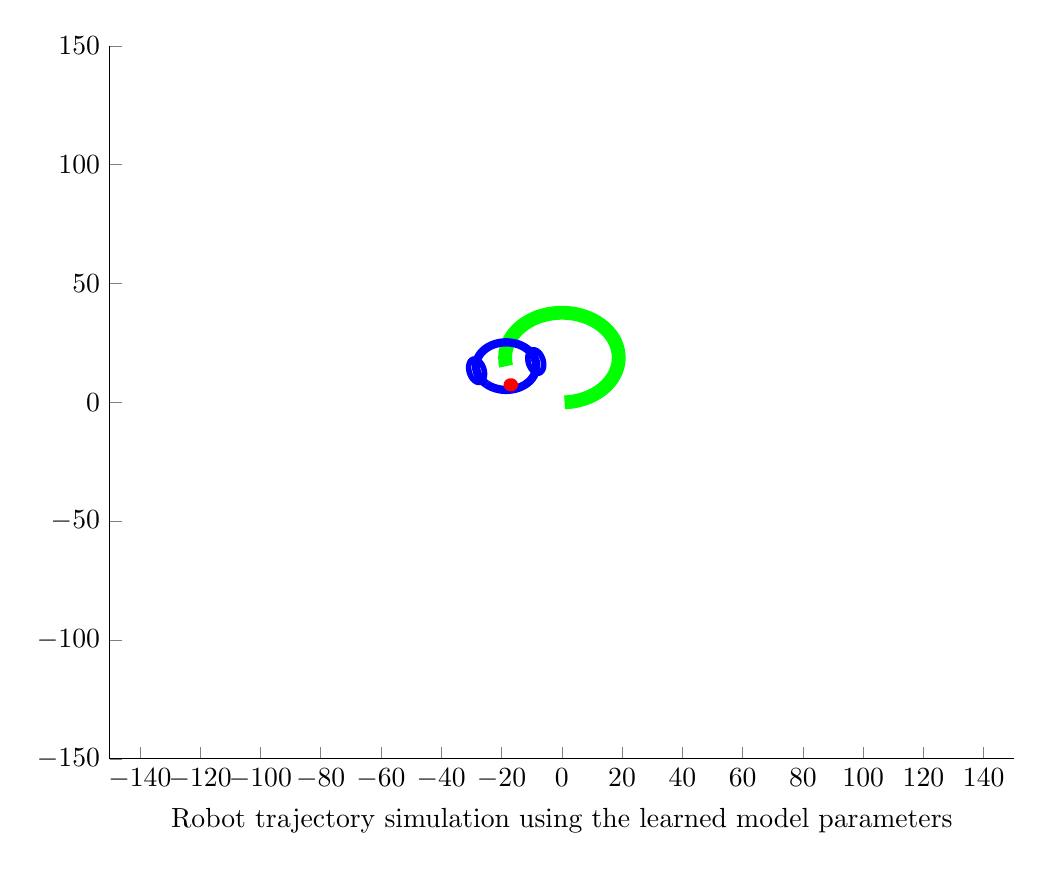
\begin{tikzpicture}

\begin{axis}[%
width=4.520833in,
height=3.565625in,
at={(0.758333in,0.48125in)},
scale only axis,
every outer x axis line/.append style={black},
every x tick label/.append style={font=\color{black}},
xmin=-150,
xmax=150,
xlabel={Robot trajectory simulation using the learned model parameters},
every outer y axis line/.append style={black},
every y tick label/.append style={font=\color{black}},
ymin=-150,
ymax=150,
axis x line*=bottom,
axis y line*=left
]
\addplot [color=green,solid,line width=5.0pt,forget plot]
  table[row sep=crcr]{%
0.924377014749405	0.0206055261941212\\
1.84663080569155	0.0865251605953999\\
2.76454135874186	0.197600223978813\\
3.67589911469206	0.353563340696163\\
4.57851028797663	0.554039082292519\\
5.47020214746965	0.798544871223251\\
6.3488282466001	1.08649214249625\\
7.21227359019604	1.41718776044309\\
8.05845972562017	1.78983568720874\\
8.8853497459416	2.20353889894341\\
9.69095319310036	2.65730154508419\\
10.473330849262	3.15003134552836\\
11.2305994048287	3.68054221992838\\
11.9609359918701	4.24755714277919\\
12.6625825720613	4.84971121742515\\
13.3338501685657	5.48555496158717\\
13.9731229316753	6.15355779650104\\
14.5788620284225	6.85211173126815\\
15.1496093468001	7.57953523354973\\
15.6839910056724	8.33407727728725\\
16.18072066193	9.11392155770544\\
16.6386026069253	9.91719086345173\\
17.0565346447367	10.7419515953477\\
17.4335107453327	11.5862184208751\\
17.768623466249	12.4479590531926\\
18.061066136949	13.3250991431785\\
18.3101348006106	14.2155272727255\\
18.5152299086639	15.117100037265\\
18.675857764002	16.0276472052889\\
18.7916317093893	16.9449769424479\\
18.8622730582084	17.8668810876516\\
18.8876117653037	18.7911404684693\\
18.8675868363079	19.7155302430371\\
18.8022464744647	20.6378252556122\\
18.6917479645965	21.555805392883\\
18.5363572944938	22.4672609281406\\
18.33644851464	23.369997840449\\
18.0925028378111	24.2618430960081\\
17.8051074807186	25.1406498789976\\
17.4749542504843	26.0043027593105\\
17.1028378793484	26.8507227847348\\
16.68965411162	27.6778724853287\\
16.2363975474765	28.4837607779398\\
15.7441592487992	29.2664477590644\\
15.2141241128115	30.0240493745097\\
14.647568019839	30.7547419546161\\
14.0458547620597	31.4567666041259\\
13.4104327606352	32.1284334361285\\
12.7428315791266	32.7681256398914\\
12.0446582415878	33.3743033727856\\
11.3175933641985	33.9455074669355\\
10.5633871097491	34.4803629416725\\
9.78385497471569	34.9775823133356\\
8.98087341906643	35.4359686944529\\
8.15637534931869	35.8544186748437\\
7.31234546572041	36.2319249777048\\
6.45081548475548	36.5675788842891\\
5.57385924847348	36.8605724213387\\
4.68358773241629	37.1102003060071\\
3.7821439641585	37.3158616435889\\
2.87169786469325	37.4770613739711\\
1.95444102508141	37.5934114633224\\
1.03258143093723	37.6646318381536\\
0.108338147449841	37.6905510594999\\
-0.816064022265764	37.6711067356022\\
-1.73839989262971	37.6063456720938\\
-2.65644925197899	37.4964237593323\\
-3.56800220697608	37.3416055971457\\
-4.4708645021798	37.1422638578982\\
-5.36286280197313	36.8988783894072\\
-6.24184992213367	36.6120350598724\\
-7.10570999845346	36.2824243475957\\
-7.95236357996643	35.9108396788888\\
-8.77977263452332	35.4981755181672\\
-9.58594545466479	35.0454252148301\\
-10.3689414519835	34.553678612107\\
-11.1268758284344	34.0241194236298\\
-11.8579241133486	33.4580223840413\\
-12.5603265552292	32.8567501805038\\
-13.2323923577583	32.2217501724898\\
-13.8725037498168	31.5545509077543\\
-14.4791198797216	30.8567584428723\\
-15.0507805243047	30.1300524772014\\
-15.5861096039066	29.3761823095735\\
-16.0838184948228	28.5969626274493\\
-16.5427091312294	27.7942691386723\\
-16.9616768891215	26.9700340563361\\
-17.3397132453219	26.1262414476357\\
-17.6759082051592	25.2649224578957\\
-17.969452492973	24.3881504212758\\
-18.2196395001702	23.4980358699193\\
-18.4258669861474	22.5967214535616\\
-18.5876385279806	21.6863767818248\\
-18.7045647153959	20.7691932016167\\
-18.7763640881429	19.8473785222044\\
-18.8028638135151	18.9231517006601\\
-18.7840001023862	17.9987375004721\\
-18.7198183627608	17.0763611361796\\
-18.6104730904701	16.1582429169211\\
-18.4562274972751	15.246592901791\\
};
\addplot [color=blue,solid,line width=3.0pt,forget plot]
  table[row sep=crcr]{%
-8.45622749727512	15.246592901791\\
-8.4562324972747	15.2565929001244\\
-8.45624749726845	15.2665928884577\\
-8.45627249724136	15.276592856791\\
-8.45630749716845	15.2865927951244\\
-8.4563524970147	15.2965926934579\\
-8.45640749673512	15.3065925417917\\
-8.4564724962747	15.3165923301258\\
-8.45654749556845	15.3265920484604\\
-8.45663249454137	15.3365916867959\\
-8.45672749310846	15.3465912351327\\
-8.45683249117472	15.3565906834711\\
-8.45694748863516	15.3665900218118\\
-8.45707248537477	15.3765892401553\\
-8.45720748126855	15.3865883285025\\
-8.45735247618152	15.3965872768543\\
-8.45750746996868	15.4065860752117\\
-8.45767246247503	15.416584713576\\
-8.45784745353559	15.4265831819485\\
-8.45803244297535	15.4365814703307\\
-8.45822743060934	15.4465795687244\\
-8.45843241624256	15.4565774671314\\
-8.45864739967002	15.4665751555538\\
-8.45887238067676	15.476572623994\\
-8.45910735903777	15.4865698624546\\
-8.45935233451809	15.4965668609381\\
-8.45960730687274	15.5065636094478\\
-8.45987227584675	15.5165600979867\\
-8.46014724117514	15.5265563165585\\
-8.46043220258296	15.5365522551669\\
-8.46072715978524	15.546547903816\\
-8.46103211248703	15.5565432525101\\
-8.46134706038336	15.5665382912538\\
-8.4616720031593	15.5765330100522\\
-8.4620069404899	15.5865273989105\\
-8.46235187204023	15.5965214478344\\
-8.46270679746535	15.6065151468297\\
-8.46307171641033	15.6165084859028\\
-8.46344662851027	15.6265014550604\\
-8.46383153339024	15.6364940443094\\
-8.46422643066534	15.6464862436574\\
-8.46463131994067	15.656478043112\\
-8.46504620081135	15.6664694326815\\
-8.46547107286249	15.6764604023745\\
-8.46590593566923	15.6864509422001\\
-8.46635078879669	15.6964410421676\\
-8.46680563180003	15.7064306922871\\
-8.4672704642244	15.7164198825688\\
-8.46774528560498	15.7264086030235\\
-8.46823009546693	15.7363968436626\\
-8.46872489332545	15.7463845944978\\
-8.46922967868575	15.7563718455413\\
-8.46974445104303	15.766358586806\\
-8.47026920988252	15.776344808305\\
-8.47080395467947	15.7863305000521\\
-8.47134868489913	15.7963156520617\\
-8.47190339999677	15.8063002543486\\
-8.47246809941768	15.8162842969281\\
-8.47304278259715	15.8262677698164\\
-8.4736274489605	15.8362506630298\\
-8.47422209792307	15.8462329665855\\
-8.47482672889021	15.8562146705011\\
-8.47544134125729	15.8661957647951\\
-8.47606593440969	15.8761762394863\\
-8.47670050772282	15.8861560845941\\
-8.4773450605621	15.8961352901388\\
-8.477999592283	15.9061138461412\\
-8.47866410223097	15.9160917426228\\
-8.4793385897415	15.9260689696055\\
-8.4800230541401	15.9360455171122\\
-8.48071749474232	15.9460213751663\\
-8.48142191085371	15.9559965337921\\
-8.48213630176985	15.9659709830143\\
-8.48286066677636	15.9759447128584\\
-8.48359500514887	15.9859177133508\\
-8.48433931615304	15.9958899745184\\
-8.48509359904456	16.0058614863891\\
-8.48585785306915	16.0158322389912\\
-8.48663207746255	16.025802222354\\
-8.48741627145054	16.0357714265076\\
-8.48821043424892	16.0457398414827\\
-8.48901456506354	16.055707457311\\
-8.48982866309026	16.0656742640248\\
-8.49065272751498	16.0756402516572\\
-8.49148675751364	16.0856054102424\\
-8.49233075225221	16.0955697298152\\
-8.4931847108867	16.1055332004112\\
-8.49404863256314	16.1154958120669\\
-8.49492251641761	16.1254575548199\\
-8.49580636157624	16.1354184187082\\
-8.49670016715517	16.1453783937711\\
-8.49760393226061	16.1553374700486\\
-8.49851765598877	16.1652956375816\\
-8.49944133742595	16.175252886412\\
-8.50037497564846	16.1852092065824\\
-8.50131856972266	16.1951645881366\\
-8.50227211870496	16.2051190211192\\
-8.50323562164181	16.2150724955757\\
-8.50420907756971	16.2250250015528\\
-8.50519248551519	16.2349765290978\\
-8.50618584449486	16.2449270682593\\
-8.50718915351535	16.2548766090867\\
-8.50820241157336	16.2648251416305\\
-8.50922561765562	16.2747726559421\\
-8.51025877073893	16.284719142074\\
-8.51130186979014	16.2946645900798\\
-8.51235491376615	16.304608990014\\
-8.51341790161391	16.3145523319322\\
-8.51449083227045	16.3244946058911\\
-8.51557370466282	16.3344358019483\\
-8.51666651770815	16.3443759101628\\
-8.51776927031363	16.3543149205943\\
-8.51888196137651	16.3642528233039\\
-8.5200045897841	16.3741896083536\\
-8.52113715441377	16.3841252658068\\
-8.52227965413296	16.3940597857277\\
-8.52343208779916	16.4039931581817\\
-8.52459445425994	16.4139253732357\\
-8.52576675235293	16.4238564209572\\
-8.52694898090585	16.4337862914154\\
-8.52814113873645	16.4437149746802\\
-8.52934322465259	16.4536424608231\\
-8.53055523745217	16.4635687399165\\
-8.53177717592318	16.4734938020342\\
-8.53300903884369	16.4834176372511\\
-8.53425082498183	16.4933402356433\\
-8.53550253309581	16.5032615872883\\
-8.53676416193393	16.5131816822647\\
-8.53803571023456	16.5231005106525\\
-8.53931717672615	16.5330180625328\\
-8.54060856012723	16.542934327988\\
-8.54190985914643	16.5528492971019\\
-8.54322107248244	16.5627629599595\\
-8.54454219882404	16.5726753066471\\
-8.54587323685012	16.5825863272525\\
-8.54721418522964	16.5924960118645\\
-8.54856504262164	16.6024043505735\\
-8.54992580767526	16.6123113334713\\
-8.55129647902976	16.6222169506506\\
-8.55267705531444	16.6321211922061\\
-8.55406753514874	16.6420240482334\\
-8.55546791714218	16.6519255088296\\
-8.55687819989438	16.6618255640934\\
-8.55829838199504	16.6717242041246\\
-8.559728462024	16.6816214190246\\
-8.56116843855117	16.6915171988963\\
-8.56261831013657	16.7014115338437\\
-8.56407807533033	16.7113044139727\\
-8.56554773267269	16.7211958293903\\
-8.567027280694	16.731085770205\\
-8.56851671791469	16.740974226527\\
-8.57001604284534	16.7508611884678\\
-8.57152525398662	16.7607466461405\\
-8.57304434982932	16.7706305896595\\
-8.57457332885435	16.780513009141\\
-8.57611218953272	16.7903938947025\\
-8.57766093032557	16.8002732364631\\
-8.57921954968417	16.8101510245435\\
-8.58078804604989	16.8200272490659\\
-8.58236641785424	16.8299019001541\\
-8.58395466351885	16.8397749679335\\
-8.58555278145546	16.8496464425309\\
-8.58716077006597	16.8595163140749\\
-8.58877862774239	16.8693845726956\\
-8.59040635286685	16.8792512085248\\
-8.59204394381164	16.8891162116958\\
-8.59369139893916	16.8989795723437\\
-8.59534871660195	16.908841280605\\
-8.5970158951427	16.9187013266181\\
-8.59869293289423	16.9285597005229\\
-8.60037982817951	16.938416392461\\
-8.60207657931163	16.9482713925758\\
-8.60378318459385	16.9581246910122\\
-8.60549964231956	16.967976277917\\
-8.60722595077231	16.9778261434385\\
-8.60896210822578	16.987674277727\\
-8.61070811294382	16.9975206709342\\
-8.61246396318042	17.0073653132138\\
-8.61422965717974	17.0172081947211\\
-8.61600519317608	17.0270493056133\\
-8.6177905693939	17.0368886360493\\
-8.61958578404783	17.0467261761896\\
-8.62139083534265	17.0565619161968\\
-8.62320572147332	17.0663958462352\\
-8.62503044062494	17.0762279564708\\
-8.6268649909728	17.0860582370714\\
-8.62870937068235	17.0958866782069\\
-8.6305635779092	17.1057132700488\\
-8.63242761079916	17.1155380027704\\
-8.63430146748818	17.1253608665471\\
-8.63618514610241	17.135181851556\\
-8.63807864475818	17.1450009479761\\
-8.63998196156198	17.1548181459883\\
-8.6418950946105	17.1646334357755\\
-8.6438180419906	17.1744468075222\\
-8.64575080177934	17.1842582514152\\
-8.64769337204396	17.1940677576431\\
-8.64964575084189	17.2038753163962\\
-8.65160793622075	17.2136809178671\\
-8.65357992621835	17.2234845522501\\
-8.6555617188627	17.2332862097416\\
-8.65755331217202	17.24308588054\\
-8.6595547041547	17.2528835548456\\
-8.66156589280936	17.2626792228607\\
-8.66358687612481	17.2724728747897\\
-8.66561765208007	17.2822645008388\\
-8.66765821864435	17.2920540912165\\
-8.6697085737771	17.3018416361332\\
-8.67176871542795	17.3116271258013\\
-8.67383864153677	17.3214105504354\\
-8.67591835003363	17.331191900252\\
-8.67800783883883	17.3409711654698\\
-8.68010710586286	17.3507483363095\\
-8.68221614900648	17.3605234029939\\
-8.68433496616063	17.370296355748\\
-8.68646355520649	17.3800671847988\\
-8.68860191401548	17.3898358803756\\
-8.69075004044925	17.3996024327095\\
-8.69290793235965	17.4093668320341\\
-8.69507558758881	17.4191290685849\\
-8.69725300396906	17.4288891325997\\
-8.69944017932299	17.4386470143185\\
-8.70163711146343	17.4484027039834\\
-8.70384379819344	17.4581561918386\\
-8.70606023730634	17.4679074681307\\
-8.70828642658568	17.4776565231085\\
-8.71052236380529	17.4874033470228\\
-8.71276804672921	17.4971479301268\\
-8.71502347311177	17.5068902626761\\
-8.71728864069755	17.5166303349281\\
-8.71956354722137	17.5263681371429\\
-8.72184819040833	17.5361036595827\\
-8.72414256797378	17.5458368925118\\
-8.72644667762335	17.5555678261972\\
-8.72876051705293	17.5652964509079\\
-8.73108408394869	17.5750227569152\\
-8.73341737598704	17.5847467344928\\
-8.7357603908347	17.5944683739168\\
-8.73811312614867	17.6041876654656\\
-8.74047557957619	17.6139045994197\\
-8.74284774875482	17.6236191660624\\
-8.74522963131239	17.633331355679\\
-8.74762122486701	17.6430411585573\\
-8.75002252702711	17.6527485649876\\
-8.75243353539136	17.6624535652624\\
-8.75485424754876	17.6721561496767\\
-8.75728466107861	17.681856308528\\
-8.75972477355048	17.6915540321162\\
-8.76217458252427	17.7012493107433\\
-8.76463408555017	17.7109421347143\\
-8.76710328016867	17.7206324943363\\
-8.76958216391058	17.7303203799188\\
-8.77207073429701	17.7400057817741\\
-8.77456898883941	17.7496886902167\\
-8.7770769250395	17.7593690955637\\
-8.77959454038936	17.7690469881348\\
-8.78212183237137	17.778722358252\\
-8.78465879845824	17.7883951962399\\
-8.787205436113	17.7980654924258\\
-8.78976174278902	17.8077332371392\\
-8.79232771592998	17.8173984207126\\
-8.79490335296993	17.8270610334806\\
-8.79748865133321	17.8367210657807\\
-8.80008360843453	17.8463785079529\\
-8.80268822167893	17.8560333503397\\
-8.80530248846181	17.8656855832863\\
-8.80792640616889	17.8753351971404\\
-8.81055997217626	17.8849821822524\\
-8.81320318385036	17.8946265289753\\
-8.81585603854795	17.9042682276649\\
-8.81851853361621	17.9139072686793\\
-8.82119066639263	17.9235436423796\\
-8.82387243420507	17.9331773391294\\
-8.82656383437178	17.942808349295\\
-8.82926486420134	17.9524366632453\\
-8.83197552099274	17.9620622713521\\
-8.83469580203531	17.9716851639898\\
-8.83742570460877	17.9813053315355\\
-8.84016522598322	17.9909227643689\\
-8.84291436341915	18.0005374528727\\
-8.84567311416741	18.0101493874322\\
-8.84844147546925	18.0197585584354\\
-8.85121944455631	18.0293649562732\\
-8.85400701865062	18.0389685713391\\
-8.85680419496461	18.0485693940297\\
-8.85961097070111	18.058167414744\\
-8.86242734305333	18.067762623884\\
-8.8652533092049	18.0773550118545\\
-8.86808886632986	18.0869445690631\\
-8.87093401159266	18.0965312859203\\
-8.87378874214814	18.1061151528394\\
-8.87665305514158	18.1156961602364\\
-8.87952694770867	18.1252742985304\\
-8.8824104169755	18.1348495581433\\
-8.88530346005862	18.1444219294998\\
-8.88820607406498	18.1539914030274\\
-8.89111825609196	18.1635579691569\\
-8.89404000322739	18.1731216183214\\
-8.89697131254951	18.1826823409576\\
-8.89991218112702	18.1922401275045\\
-8.90286260601906	18.2017949684044\\
-8.90582258427518	18.2113468541025\\
-8.90879211293543	18.2208957750469\\
-8.91177118903026	18.2304417216887\\
-8.91475980958061	18.239984684482\\
-8.91775797159784	18.2495246538836\\
-8.92076567208381	18.2590616203538\\
-8.92378290803081	18.2685955743555\\
-8.92680967642161	18.2781265063548\\
-8.92984597422943	18.2876544068208\\
-8.93289179841798	18.2971792662255\\
-8.93594714594144	18.306701075044\\
-8.93901201374445	18.3162198237547\\
-8.94208639876216	18.3257355028387\\
-8.94517029792017	18.3352481027803\\
-8.94826370813458	18.344757614067\\
-8.951366626312	18.3542640271893\\
-8.95447904934949	18.3637673326407\\
-8.95760097413464	18.3732675209179\\
-8.96073239754552	18.3827645825208\\
-8.96387331645071	18.3922585079522\\
-8.96702372770929	18.4017492877183\\
-8.97018362817084	18.4112369123283\\
-8.97335301467548	18.4207213722945\\
-8.97653188405381	18.4302026581325\\
-8.97972023312696	18.439680760361\\
-8.98291805870658	18.449155669502\\
-8.98612535759486	18.4586273760804\\
-8.98934212658448	18.4680958706246\\
-8.99256836245869	18.4775611436662\\
-8.99580406199125	18.4870231857397\\
-8.99904922194645	18.4964819873832\\
-9.00230383907913	18.505937539138\\
-9.00556791013469	18.5153898315483\\
-9.00884143184905	18.524838855162\\
-9.01212440094869	18.5342846005301\\
-9.01541681415063	18.5437270582066\\
-9.01871866816247	18.5531662187494\\
-9.02202995968236	18.562602072719\\
-9.02535068539899	18.5720346106798\\
-9.02868084199165	18.5814638231992\\
-9.03202042613018	18.5908897008479\\
-9.035369434475	18.6003122342001\\
-9.0387278636771	18.6097314138332\\
-9.04209571037804	18.6191472303281\\
-9.04547297120999	18.6285596742689\\
-9.04885964279567	18.6379687362433\\
-9.05225572174843	18.6473744068421\\
-9.05566120467218	18.6567766766597\\
-9.05907608816144	18.6661755362938\\
-9.06250036880133	18.6755709763455\\
-9.06593404316756	18.6849629874195\\
-9.06937710782646	18.6943515601237\\
-9.07282955933497	18.7037366850694\\
-9.07629139424064	18.7131183528717\\
-9.07976260908162	18.7224965541489\\
-9.08324320038672	18.7318712795226\\
-9.08673316467533	18.7412425196183\\
-9.09023249845749	18.7506102650647\\
-9.09374119823387	18.7599745064939\\
-9.09725926049577	18.7693352345419\\
-9.10078668172512	18.7786924398479\\
-9.10432345839451	18.7880461130545\\
-9.10786958696717	18.7973962448083\\
-9.11142506389695	18.806742825759\\
-9.11498988562838	18.8160858465601\\
-9.11856404859665	18.8254252978686\\
-9.1221475492276	18.8347611703449\\
-9.12574038393771	18.8440934546533\\
-9.12934254913415	18.8534221414615\\
-9.13295404121477	18.8627472214406\\
-9.13657485656807	18.8720686852658\\
-9.14020499157323	18.8813865236155\\
-9.14384444260012	18.8907007271719\\
-9.14749320600929	18.9000112866207\\
-9.15115127815197	18.9093181926515\\
-9.1548186553701	18.9186214359573\\
-9.1584953339963	18.9279210072348\\
-9.16218131035388	18.9372168971846\\
-9.16587658075687	18.9465090965107\\
-9.16958114151001	18.9557975959208\\
-9.17329498890873	18.9650823861266\\
-9.17701811923919	18.9743634578433\\
-9.18075052877825	18.9836408017896\\
-9.1844922137935	18.9929144086884\\
-9.18824317054327	19.002184269266\\
-9.19200339527659	19.0114503742526\\
-9.19577288423324	19.020712714382\\
-9.19955163364373	19.0299712803918\\
-9.20333963972931	19.0392260630237\\
-9.20713689870198	19.0484770530226\\
-9.21094340676448	19.0577242411378\\
-9.2147591601103	19.0669676181219\\
-9.21858415492369	19.0762071747316\\
-9.22241838737964	19.0854429017274\\
-9.22626185364394	19.0946747898735\\
-9.23011454987312	19.103902829938\\
-9.23397647221447	19.1131270126929\\
-9.23784761680608	19.122347328914\\
-9.2417279797768	19.131563769381\\
-9.24561755724626	19.1407763248775\\
-9.24951634532491	19.1499849861909\\
-9.25342434011393	19.1591897441125\\
-9.25734153770535	19.1683905894376\\
-9.26126793418196	19.1775875129654\\
-9.26520352561737	19.1867805054988\\
-9.26914830807598	19.195969557845\\
-9.27310227761302	19.2051546608149\\
-9.27706543027451	19.2143358052233\\
-9.2810377620973	19.2235129818891\\
-9.28501926910906	19.2326861816352\\
-9.28900994732829	19.2418553952884\\
-9.29300979276431	19.2510206136794\\
-9.29701880141726	19.260181827643\\
-9.30103696927815	19.2693390280181\\
-9.3050642923288	19.2784922056473\\
-9.30910076654189	19.2876413513776\\
-9.31314638788096	19.2967864560597\\
-9.31720115230037	19.3059275105486\\
-9.32126505574536	19.3150645057033\\
-9.32533809415203	19.3241974323867\\
-9.32942026344735	19.3333262814659\\
-9.33351155954914	19.3424510438121\\
-9.33761197836611	19.3515717103005\\
-9.34172151579783	19.3606882718104\\
-9.34584016773478	19.3698007192253\\
-9.3499679300583	19.3789090434327\\
-9.35410479864062	19.3880132353243\\
-9.35825076934489	19.3971132857959\\
-9.36240583802513	19.4062091857475\\
-9.36657000052626	19.4153009260831\\
-9.37074325268414	19.4243884977111\\
-9.37492559032551	19.4334718915438\\
-9.37911700926802	19.4425510984979\\
-9.38331750532027	19.4516261094941\\
-9.38752707428175	19.4606969154575\\
-9.3917457119429	19.4697635073172\\
-9.39597341408508	19.4788258760067\\
-9.40021017648059	19.4878840124635\\
-9.40445599489266	19.4969379076296\\
-9.40871086507548	19.505987552451\\
-9.41297478277418	19.5150329378781\\
-9.41724774372484	19.5240740548656\\
-9.4215297436545	19.5331108943723\\
-9.42582077828117	19.5421434473613\\
-9.43012084331379	19.5511717048001\\
-9.43442993445233	19.5601956576605\\
-9.43874804738767	19.5692152969185\\
-9.4430751778017	19.5782306135544\\
-9.44741132136731	19.587241598553\\
-9.45175647374835	19.5962482429033\\
-9.45611063059965	19.6052505375986\\
-9.46047378756708	19.6142484736366\\
-9.46484594028746	19.6232420420194\\
-9.46922708438865	19.6322312337535\\
-9.4736172154895	19.6412160398496\\
-9.47801632919989	19.6501964513228\\
-9.4824244211207	19.659172459193\\
-9.48684148684384	19.6681440544839\\
-9.49126752195223	19.677111228224\\
-9.49570252201986	19.6860739714462\\
-9.50014648261172	19.6950322751877\\
-9.50459939928384	19.7039861304902\\
-9.50906126758332	19.7129355283998\\
-9.51353208304828	19.7218804599672\\
-9.51801184120791	19.7308209162474\\
-9.52250053758245	19.7397568882999\\
-9.52699816768321	19.7486883671888\\
-9.53150472701255	19.7576153439827\\
-9.53602021106392	19.7665378097545\\
-9.54054461532183	19.7754557555817\\
-9.54507793526188	19.7843691725465\\
-9.54962016635075	19.7932780517353\\
-9.5541713040462	19.8021823842395\\
-9.55873134379711	19.8110821611545\\
-9.56330028104343	19.8199773735806\\
-9.56787811121623	19.8288680126226\\
-9.57246482973767	19.8377540693899\\
-9.57706043202104	19.8466355349964\\
-9.58166491347074	19.8555124005607\\
-9.58627826948227	19.8643846572058\\
-9.5909004954423	19.8732522960596\\
-9.59553158672859	19.8821153082544\\
-9.60017153871005	19.8909736849272\\
-9.60482034674674	19.8998274172195\\
-9.60947800618983	19.9086764962777\\
-9.61414451238168	19.9175209132528\\
-9.61881986065578	19.9263606593002\\
-9.62350404633678	19.9351957255802\\
-9.62819706474049	19.9440261032578\\
-9.6328989111739	19.9528517835026\\
-9.63760958093516	19.9616727574889\\
-9.6423290693136	19.9704890163957\\
-9.64705737158974	19.9793005514069\\
-9.65179448303527	19.9881073537107\\
-9.65654039891307	19.9969094145005\\
-9.66129511447725	20.0057067249742\\
-9.66605862497307	20.0144992763345\\
-9.67083092563703	20.0232870597888\\
-9.67561201169683	20.0320700665493\\
-9.68040187837139	20.0408482878331\\
-9.68520052087083	20.0496217148618\\
-9.69000793439652	20.0583903388622\\
-9.69482411414104	20.0671541510655\\
-9.69964905528822	20.075913142708\\
-9.7044827530131	20.0846673050306\\
-9.709325202482	20.0934166292793\\
-9.71417639885247	20.1021611067046\\
-9.71903633727331	20.1109007285621\\
-9.72390501288458	20.1196354861122\\
-9.7287824208176	20.1283653706201\\
-9.73366855619498	20.1370903733559\\
-9.73856341413057	20.1458104855947\\
-9.74346698972951	20.1545256986164\\
-9.74837927808824	20.1632360037056\\
-9.75330027429446	20.1719413921521\\
-9.75822997342718	20.1806418552506\\
-9.7631683705567	20.1893373843005\\
-9.76811546074462	20.1980279706063\\
-9.77307123904385	20.2067136054775\\
-9.77803570049862	20.2153942802284\\
-9.78300884014446	20.2240699861783\\
-9.78799065300823	20.2327407146516\\
-9.79298113410813	20.2414064569774\\
-9.79798027845367	20.2500672044902\\
-9.8029880810457	20.258722948529\\
-9.80800453687643	20.2673736804382\\
-9.8130296409294	20.2760193915671\\
-9.81806338817951	20.2846600732698\\
-9.823105773593	20.2932957169059\\
-9.8281567921275	20.3019263138395\\
-9.83321643873199	20.3105518554401\\
-9.83828470834682	20.3191723330822\\
-9.84336159590371	20.3277877381453\\
-9.8484470963258	20.336398062014\\
-9.85354120452756	20.345003296078\\
-9.8586439154149	20.353603431732\\
-9.8637552238851	20.3621984603758\\
-9.86887512482687	20.3707883734146\\
-9.87400361312029	20.3793731622583\\
-9.87914068363687	20.3879528183222\\
-9.88428633123956	20.3965273330265\\
-9.8894405507827	20.4050966977969\\
-9.89460333711207	20.4136609040639\\
-9.89977468506489	20.4222199432634\\
-9.90495458946981	20.4307738068362\\
-9.91014304514692	20.4393224862285\\
-9.91534004690777	20.4478659728918\\
-9.92054558955537	20.4564042582823\\
-9.92575966788415	20.464937333862\\
-9.93098227668006	20.4734651910976\\
-9.93621341072047	20.4819878214614\\
-9.94145306477427	20.4905052164307\\
-9.94670123360178	20.4990173674882\\
-9.95195791195485	20.5075242661216\\
-9.9572230945768	20.516025903824\\
-9.96249677620244	20.524522272094\\
-9.9677789515581	20.5330133624349\\
-9.97306961536159	20.5414991663559\\
-9.97836876232226	20.549979675371\\
-9.98367638714095	20.5584548809999\\
-9.98899248451006	20.5669247747671\\
-9.99431704911346	20.575389348203\\
-9.99965007562661	20.5838485928428\\
-10.0049915587165	20.5923025002274\\
-10.0103414930416	20.6007510619029\\
-10.015699873252	20.6091942694206\\
-10.0210666939893	20.6176321143374\\
-10.0264419498867	20.6260645882154\\
-10.031825635569	20.6344916826222\\
-10.0372177456524	20.6429133891307\\
-10.0426182747449	20.6513296993191\\
-10.0480272174459	20.6597406047712\\
-10.0534445683465	20.6681460970761\\
-10.0588703220293	20.6765461678282\\
-10.0643044730686	20.6849408086274\\
-10.0697470160302	20.6933300110793\\
-10.0751979454716	20.7017137667944\\
-10.0806572559418	20.7100920673892\\
-10.0861249419816	20.7184649044853\\
-10.0916009981232	20.7268322697098\\
-10.0970854188907	20.7351941546953\\
-10.1025781987995	20.7435505510801\\
-10.108079332357	20.7519014505077\\
-10.1135888140619	20.7602468446273\\
-10.1191066384047	20.7685867250933\\
-10.1246327998678	20.776921083566\\
-10.1301672929248	20.7852499117109\\
-10.1357101120414	20.7935732011993\\
-10.1412612516747	20.8018909437079\\
-10.1468207062735	20.8102031309189\\
-10.1523884702784	20.8185097545201\\
-10.1579645381216	20.8268108062049\\
-10.1635489042271	20.8351062776723\\
-10.1691415630106	20.8433961606268\\
-10.1747425088792	20.8516804467785\\
-10.1803517362322	20.8599591278431\\
-10.1859692394602	20.8682321955419\\
-10.1915950129458	20.8764996416019\\
-10.1972290510632	20.8847614577557\\
-10.2028713481783	20.8930176357414\\
-10.2085218986489	20.9012681673028\\
-10.2141806968245	20.9095130441894\\
-10.2198477370461	20.9177522581563\\
-10.2255230136468	20.9259858009644\\
-10.2312065209513	20.93421366438\\
-10.2368982532761	20.9424358401754\\
-10.2425982049295	20.9506523201282\\
-10.2483063702114	20.9588630960222\\
-10.2540227434138	20.9670681596464\\
-10.2597473188203	20.9752675027958\\
-10.2654800907063	20.9834611172711\\
-10.271221053339	20.9916489948787\\
-10.2769702009775	20.9998311274307\\
-10.2827275278725	21.0080075067449\\
-10.2884930282669	21.016178124645\\
-10.294266696395	21.0243429729603\\
-10.3000485264833	21.0325020435261\\
-10.3058385127499	21.0406553281832\\
-10.3116366494047	21.0488028187783\\
-10.3174429306498	21.0569445071641\\
-10.3232573506787	21.0650803851987\\
-10.3290799036771	21.0732104447463\\
-10.3349105838224	21.0813346776768\\
-10.340749385284	21.0894530758661\\
-10.3465963022229	21.0975656311956\\
-10.3524513287924	21.105672335553\\
-10.3583144591374	21.1137731808313\\
-10.3641856873948	21.1218681589299\\
-10.3700650076933	21.1299572617538\\
-10.3759524141536	21.1380404812137\\
-10.3818479008883	21.1461178092266\\
-10.387751462002	21.154189237715\\
-10.393663091591	21.1622547586076\\
-10.3995827837437	21.1703143638389\\
-10.4055105325405	21.1783680453491\\
-10.4114463320536	21.1864157950848\\
-10.4173901763471	21.194457604998\\
-10.4233420594774	21.202493467047\\
-10.4293019754923	21.210523373196\\
-10.4352699184322	21.2185473154149\\
-10.4412458823289	21.22656528568\\
-10.4472298612066	21.2345772759732\\
-10.4532218490813	21.2425832782825\\
-10.459221839961	21.2505832846019\\
-10.4652298278456	21.2585772869314\\
-10.4712458067273	21.2665652772771\\
-10.4772697705899	21.2745472476509\\
-10.4833017134097	21.2825231900708\\
-10.4893416291545	21.290493096561\\
-10.4953895117846	21.2984569591514\\
-10.5014453552519	21.3064147698783\\
-10.5075091535008	21.3143665207839\\
-10.5135809004673	21.3223122039163\\
-10.5196605900798	21.3302518113299\\
-10.5257482162585	21.3381853350852\\
-10.5318437729159	21.3461127672485\\
-10.5379472539563	21.3540340998924\\
-10.5440586532762	21.3619493250957\\
-10.5501779647644	21.369858434943\\
-10.5563051823015	21.3777614215254\\
-10.5624402997602	21.3856582769397\\
-10.5685833110054	21.3935489932891\\
-10.5747342098942	21.401433562683\\
-10.5808929902756	21.4093119772367\\
-10.5870596459908	21.4171842290719\\
-10.5932341708733	21.4250503103162\\
-10.5994165587484	21.4329102131037\\
-10.6056068034338	21.4407639295744\\
-10.6118048987392	21.4486114518745\\
-10.6180108384666	21.4564527721566\\
-10.62422461641	21.4642878825794\\
-10.6304462263556	21.4721167753077\\
-10.6366756620819	21.4799394425126\\
-10.6429129173593	21.4877558763716\\
-10.6491579859506	21.495566069068\\
-10.6554108616109	21.5033700127918\\
-10.6616715380871	21.5111676997391\\
-10.6679400091186	21.518959122112\\
-10.6742162684369	21.5267442721193\\
-10.6805003097658	21.5345231419757\\
-10.6867921268213	21.5422957239024\\
-10.6930917133115	21.5500620101268\\
-10.6993990629368	21.5578219928826\\
-10.7057141693899	21.5655756644099\\
-10.7120370263557	21.5733230169549\\
-10.7183676275114	21.5810640427703\\
-10.7247059665262	21.5887987341151\\
-10.7310520370619	21.5965270832546\\
-10.7374058327725	21.6042490824605\\
-10.7437673473041	21.6119647240107\\
-10.7501365742951	21.6196740001896\\
-10.7565135073765	21.627376903288\\
-10.7628981401712	21.6350734256028\\
-10.7692904662946	21.6427635594377\\
-10.7756904793544	21.6504472971025\\
-10.7820981729506	21.6581246309134\\
-10.7885135406755	21.6657955531931\\
-10.7949365761137	21.6734600562707\\
-10.8013672728422	21.6811181324817\\
-10.8078056244302	21.6887697741679\\
-10.8142516244395	21.6964149736779\\
-10.8207052664241	21.7040537233663\\
-10.8271665439302	21.7116860155944\\
-10.8336354504966	21.7193118427299\\
-10.8401119796545	21.7269311971471\\
-10.8465961249272	21.7345440712265\\
-10.8530878798307	21.7421504573552\\
-10.8595872378732	21.749750347927\\
-10.8660941925553	21.7573437353418\\
-10.87260873737	21.7649306120064\\
-10.8791308658029	21.7725109703338\\
-10.8856605713318	21.7800848027436\\
-10.892197847427	21.7876521016621\\
-10.8987426875512	21.795212859522\\
-10.9052950851596	21.8027670687624\\
-10.9118550336998	21.8103147218292\\
-10.9184225266118	21.8178558111748\\
-10.9249975573281	21.825390329258\\
-10.9315801192738	21.8329182685443\\
-10.9381702058662	21.8404396215058\\
-10.9447678105152	21.8479543806211\\
-10.9513729266234	21.8554625383755\\
-10.9579855475855	21.8629640872608\\
-10.9646056667889	21.8704590197754\\
-10.9712332776135	21.8779473284245\\
-10.9778683734317	21.8854290057197\\
-10.9845109476084	21.8929040441794\\
-10.991160993501	21.9003724363285\\
-10.9978185044595	21.9078341746986\\
-11.0044834738264	21.915289251828\\
-11.0111558949367	21.9227376602616\\
-11.017835761118	21.930179392551\\
-11.0245230656904	21.9376144412544\\
-11.0312178019666	21.9450427989369\\
-11.0379199632518	21.9524644581701\\
-11.044629542844	21.9598794115322\\
-11.0513465340336	21.9672876516084\\
-11.0580709301034	21.9746891709904\\
-11.0648027243293	21.9820839622767\\
-11.0715419099792	21.9894720180725\\
-11.0782884803142	21.9968533309897\\
-11.0850424285875	22.0042278936471\\
-11.0918037480454	22.01159569867\\
-11.0985724319263	22.0189567386907\\
-11.1053484734617	22.0263110063482\\
-11.1121318658755	22.0336584942881\\
-11.1189226023843	22.0409991951629\\
-11.1257206761975	22.0483331016321\\
-11.1325260805168	22.0556602063616\\
-11.1393388085369	22.0629805020244\\
-11.1461588534451	22.0702939813001\\
-11.1529862084214	22.0776006368753\\
-11.1598208666383	22.0849004614434\\
-11.1666628212612	22.0921934477045\\
-11.1735120654482	22.0994795883656\\
-11.1803685923501	22.1067588761406\\
-11.1872323951102	22.1140313037501\\
-11.1941034668649	22.1212968639219\\
-11.2009818007429	22.1285555493902\\
-11.2078673898661	22.1358073528965\\
-11.2147602273487	22.1430522671889\\
-11.221660306298	22.1502902850226\\
-11.2285676198139	22.1575213991594\\
-11.2354821609891	22.1647456023683\\
-11.2424039229091	22.171962887425\\
-11.2493328986519	22.1791732471124\\
-11.2562690812888	22.18637667422\\
-11.2632124638835	22.1935731615444\\
-11.2701630394927	22.2007627018891\\
-11.2771208011657	22.2079452880646\\
-11.2840857419448	22.2151209128883\\
-11.291057854865	22.2222895691845\\
-11.2980371329543	22.2294512497847\\
-11.3050235692334	22.2366059475271\\
-11.3120171567158	22.2437536552571\\
-11.3190178884079	22.2508943658268\\
-11.3260257573091	22.2580280720957\\
-11.3330407564114	22.26515476693\\
-11.3400628786999	22.2722744432031\\
-11.3470921171523	22.2793870937951\\
-11.3541284647396	22.2864927115936\\
-11.3611719144253	22.2935912894928\\
-11.368222459166	22.3006828203943\\
-11.3752800919112	22.3077672972064\\
-11.3823448056031	22.3148447128447\\
-11.3894165931772	22.3219150602318\\
-11.3964954475616	22.3289783322973\\
-11.4035813616774	22.3360345219779\\
-11.4106743284388	22.3430836222176\\
-11.4177743407528	22.3501256259671\\
-11.4248813915193	22.3571605261845\\
-11.4319954736314	22.3641883158348\\
-11.4391165799749	22.3712089878904\\
-11.4462447034287	22.3782225353304\\
-11.4533798368647	22.3852289511414\\
-11.4605219731478	22.3922282283169\\
-11.4676711051359	22.3992203598577\\
-11.4748272256798	22.4062053387717\\
-11.4819903276233	22.4131831580738\\
-11.4891604038035	22.4201538107862\\
-11.4963374470501	22.4271172899384\\
-11.5035214501862	22.4340735885667\\
-11.5107124060278	22.441022699715\\
-11.517910307384	22.4479646164341\\
-11.5251151470567	22.454899331782\\
-11.5323269178412	22.4618268388241\\
-11.5395456125257	22.4687471306329\\
-11.5467712238915	22.4756602002881\\
-11.554003744713	22.4825660408765\\
-11.5612431677576	22.4894646454924\\
-11.5684894857861	22.4963560072372\\
-11.575742691552	22.5032401192195\\
-11.5830027778021	22.5101169745552\\
-11.5902697372763	22.5169865663674\\
-11.5975435627077	22.5238488877865\\
-11.6048242468225	22.5307039319503\\
-11.61211178234	22.5375516920036\\
-11.6194061619726	22.5443921610988\\
-11.626707378426	22.5512253323953\\
-11.634015424399	22.55805119906\\
-11.6413302925834	22.564869754267\\
-11.6486519756645	22.5716809911977\\
-11.6559804663205	22.578484903041\\
-11.663315757223	22.5852814829929\\
-11.6706578410367	22.5920707242568\\
-11.6780067104195	22.5988526200435\\
-11.6853623580225	22.6056271635711\\
-11.69272477649	22.6123943480651\\
-11.7000939584598	22.6191541667582\\
-11.7074698965624	22.6259066128906\\
-11.7148525834222	22.63265167971\\
-11.7222420116563	22.6393893604712\\
-11.7296381738753	22.6461196484366\\
-11.737041062683	22.6528425368758\\
-11.7444506706767	22.6595580190661\\
-11.7518669904466	22.6662660882918\\
-11.7592900145765	22.6729667378449\\
-11.7667197356433	22.6796599610249\\
-11.7741561462172	22.6863457511383\\
-11.781599238862	22.6930241014996\\
-11.7890490061345	22.6996950054303\\
-11.7965054405849	22.7063584562595\\
-11.8039685347569	22.7130144473238\\
-11.8114382811872	22.7196629719671\\
-11.8189146724062	22.726304023541\\
-11.8263977009375	22.7329375954044\\
-11.833887359298	22.7395636809238\\
-11.8413836399981	22.7461822734729\\
-11.8488865355415	22.7527933664334\\
-11.8563960384253	22.7593969531939\\
-11.86391214114	22.7659930271511\\
-11.8714348361695	22.7725815817088\\
-11.8789641159912	22.7791626102784\\
-11.8864999730757	22.7857361062789\\
-11.8940423998871	22.7923020631369\\
-11.9015913888831	22.7988604742863\\
-11.9091469325147	22.8054113331688\\
-11.9167090232263	22.8119546332335\\
-11.9242776534558	22.818490367937\\
-11.9318528156346	22.8250185307438\\
-11.9394345021875	22.8315391151255\\
-11.947022705533	22.8380521145617\\
-11.9546174180826	22.8445575225393\\
-11.9622186322418	22.8510553325529\\
-11.9698263404093	22.8575455381047\\
-11.9774405349774	22.8640281327045\\
-11.985061208332	22.8705031098697\\
-11.9926883528523	22.8769704631253\\
-12.0003219609112	22.883430186004\\
-12.0079620248751	22.8898822720461\\
-12.0156085371039	22.8963267147994\\
-12.0232614899512	22.9027635078195\\
-12.0309208757639	22.9091926446697\\
-12.0385866868828	22.9156141189208\\
-12.0462589156419	22.9220279241513\\
-12.053937554369	22.9284340539474\\
-12.0616225953856	22.934832501903\\
-12.0693140310065	22.9412232616196\\
-12.0770118535403	22.9476063267066\\
-12.0847160552893	22.9539816907807\\
-12.0924266285492	22.9603493474667\\
-12.1001435656094	22.9667092903969\\
-12.107866858753	22.9730615132113\\
-12.1155965002568	22.9794060095578\\
-12.123332482391	22.9857427730918\\
-12.1310747974197	22.9920717974766\\
-12.1388234376005	22.9983930763832\\
-12.1465783951849	23.0047066034902\\
-12.1543396624179	23.0110123724841\\
-12.1621072315381	23.0173103770593\\
-12.1698810947782	23.0236006109176\\
-12.1776612443641	23.0298830677688\\
-12.1854476725157	23.0361577413305\\
-12.1932403714466	23.0424246253281\\
-12.2010393333642	23.0486837134945\\
-12.2088445504693	23.0549349995708\\
-12.2166560149569	23.0611784773057\\
-12.2244737190155	23.0674141404556\\
-12.2322976548273	23.0736419827849\\
-12.2401278145685	23.0798619980659\\
-12.2479641904088	23.0860741800783\\
-12.2558067745119	23.0922785226102\\
-12.2636555590352	23.098475019457\\
-12.2715105361299	23.1046636644225\\
-12.2793716979411	23.1108444513178\\
-12.2872390366076	23.1170173739622\\
-12.295112544262	23.1231824261828\\
-12.3029922130308	23.1293396018145\\
-12.3108780350344	23.1354888947002\\
-12.318770002387	23.1416302986905\\
-12.3266681071966	23.1477638076441\\
-12.334572341565	23.1538894154275\\
-12.3424826975881	23.160007115915\\
-12.3503991673554	23.166116902989\\
-12.3583217429506	23.1722187705396\\
-12.366250416451	23.178312712465\\
-12.3741851799281	23.1843987226712\\
-12.3821260254469	23.1904767950723\\
-12.3900729450667	23.1965469235902\\
-12.3980259308405	23.2026091021547\\
-12.4059849748154	23.2086633247036\\
-12.4139500690323	23.2147095851829\\
-12.4219212055261	23.220747877546\\
-12.4298983763257	23.2267781957549\\
-12.437881573454	23.2328005337792\\
-12.4458707889277	23.2388148855964\\
-12.4538660147575	23.2448212451924\\
-12.4618672429484	23.2508196065607\\
-12.469874465499	23.2568099637029\\
-12.4778876744021	23.2627923106288\\
-12.4859068616446	23.2687666413559\\
-12.4939320192072	23.2747329499099\\
-12.5019631390648	23.2806912303246\\
-12.5100002131862	23.2866414766416\\
-12.5180432335345	23.2925836829107\\
-12.5260921920665	23.2985178431897\\
-12.5341470807333	23.3044439515444\\
-12.54220789148	23.3103620020488\\
-12.5502746162459	23.3162719887847\\
-12.5583472469641	23.3221739058422\\
-12.5664257755621	23.3280677473193\\
-12.5745101939614	23.3339535073223\\
-12.5826004940774	23.3398311799654\\
-12.59069666782	23.3457007593708\\
-12.5987987070929	23.3515622396691\\
-12.6069066037941	23.3574156149987\\
-12.6150203498157	23.3632608795063\\
-12.6231399370439	23.3690980273466\\
-12.6312653573593	23.3749270526824\\
-12.6393966026363	23.3807479496848\\
-12.6475336647437	23.3865607125327\\
-12.6556765355444	23.3923653354136\\
-12.6638252068957	23.3981618125227\\
-12.6719796706487	23.4039501380636\\
-12.6801399186491	23.4097303062479\\
-12.6883059427366	23.4155023112954\\
-12.6964777347451	23.4212661474343\\
-12.704655286503	23.4270218089006\\
-12.7128385898326	23.4327692899386\\
-12.7210276365505	23.438508584801\\
-12.7292224184679	23.4442396877484\\
-12.7374229273899	23.4499625930496\\
-12.745629155116	23.4556772949819\\
-12.7538410934399	23.4613837878304\\
-12.7620587341498	23.4670820658887\\
-12.770282069028	23.4727721234586\\
-12.7785110898511	23.4784539548499\\
-12.7867457883901	23.4841275543809\\
-12.7949861564104	23.4897929163779\\
-12.8032321856716	23.4954500351755\\
-12.8114838679276	23.5010989051167\\
-12.8197411949267	23.5067395205526\\
-12.8280041584117	23.5123718758426\\
-12.8362727501196	23.5179959653543\\
-12.8445469617817	23.5236117834636\\
-12.8528267851239	23.5292193245547\\
-12.8611122118664	23.5348185830201\\
-12.8694032337236	23.5404095532605\\
-12.8776998424047	23.5459922296849\\
-12.8860020296129	23.5515666067107\\
-12.8943097870462	23.5571326787635\\
-12.9026231063967	23.5626904402772\\
-12.9109419793511	23.5682398856941\\
-12.9192663975906	23.5737810094646\\
-12.9275963527908	23.5793138060478\\
-12.9359318366216	23.5848382699107\\
-12.9442728407476	23.590354395529\\
-12.9526193568278	23.5958621773865\\
-12.9609713765157	23.6013616099753\\
-12.9693288914592	23.6068526877962\\
-12.9776918933009	23.612335405358\\
-12.9860603736778	23.617809757178\\
-12.9944343242213	23.6232757377818\\
-13.0028137365575	23.6287333417035\\
-13.0111986023071	23.6341825634855\\
-13.0195889130851	23.6396233976784\\
-13.0279846605012	23.6450558388416\\
-13.0363858361597	23.6504798815426\\
-13.0447924316594	23.6558955203572\\
-13.0532044385937	23.66130274987\\
-13.0616218485507	23.6667015646736\\
-13.0700446531128	23.6720919593692\\
-13.0784728438573	23.6774739285665\\
-13.086906412356	23.6828474668835\\
-13.0953453501754	23.6882125689466\\
-13.1037896488765	23.6935692293907\\
-13.1122393000149	23.6989174428592\\
-13.1206942951412	23.7042572040039\\
-13.1291546258002	23.709588507485\\
-13.1376202835316	23.7149113479712\\
-13.1460912598697	23.7202257201396\\
-13.1545675463437	23.7255316186759\\
-13.1630491344772	23.7308290382743\\
-13.1715360157886	23.7361179736371\\
-13.180028181791	23.7413984194757\\
-13.1885256239924	23.7466703705094\\
-13.1970283338951	23.7519338214663\\
-13.2055363029966	23.7571887670831\\
-13.2140495227888	23.7624352021047\\
-13.2225679847586	23.7676731212847\\
-13.2310916803875	23.7729025193851\\
-13.2396206011517	23.7781233911767\\
-13.2481547385224	23.7833357314385\\
-13.2566940839654	23.7885395349582\\
-13.2652386289414	23.793734796532\\
-13.2737883649059	23.7989215109645\\
-13.282343283309	23.8040996730692\\
-13.2909033755959	23.8092692776678\\
-13.2994686332065	23.8144303195908\\
-13.3080390475756	23.8195827936771\\
-13.3166146101326	23.8247266947741\\
-13.3251953123022	23.8298620177381\\
-13.3337811455034	23.8349887574337\\
-13.3423721011506	23.8401069087342\\
-13.3509681706528	23.8452164665214\\
-13.3595693454139	23.8503174256857\\
-13.3681756168327	23.8554097811262\\
-13.376786976303	23.8604935277506\\
-13.3854034152133	23.865568660475\\
-13.3940249249473	23.8706351742244\\
-13.4026514968835	23.8756930639323\\
-13.4112831223952	23.8807423245407\\
-13.4199197928509	23.8857829510004\\
-13.4285614996139	23.8908149382707\\
-13.4372082340425	23.8958382813198\\
-13.4458599874899	23.9008529751242\\
-13.4545167513044	23.9058590146692\\
-13.4631785168292	23.9108563949489\\
-13.4718452754026	23.9158451109658\\
-13.4805170183578	23.9208251577312\\
-13.4891937370231	23.9257965302651\\
-13.4978754227217	23.930759223596\\
-13.506562066772	23.9357132327614\\
-13.5152536604873	23.9406585528071\\
-13.523950195176	23.945595178788\\
-13.5326516621416	23.9505231057672\\
-13.5413580526827	23.955442328817\\
-13.5500693580927	23.9603528430181\\
-13.5587855696605	23.96525464346\\
-13.5675066786698	23.9701477252409\\
-13.5762326763996	23.9750320834677\\
-13.5849635541237	23.979907713256\\
-13.5936993031114	23.9847746097302\\
-13.6024399146269	23.9896327680235\\
-13.6111853799295	23.9944821832776\\
-13.6199356902739	23.9993228506431\\
-13.6286908369096	24.0041547652795\\
-13.6374508110817	24.0089779223547\\
-13.64621560403	24.0137923170456\\
-13.6549852069898	24.0185979445378\\
-13.6637596111915	24.0233948000258\\
-13.6725388078606	24.0281828787125\\
-13.6813227882181	24.03296217581\\
-13.6901115434799	24.037732686539\\
-13.6989050648572	24.0424944061289\\
-13.7077033435566	24.0472473298181\\
-13.7165063707797	24.0519914528535\\
-13.7253141377236	24.0567267704911\\
-13.7341266355804	24.0614532779956\\
-13.7429438555377	24.0661709706405\\
-13.7517657887783	24.070879843708\\
-13.7605924264801	24.0755798924893\\
-13.7694237598167	24.0802711122844\\
-13.7782597799565	24.084953498402\\
-13.7871004780638	24.0896270461597\\
-13.7959458452976	24.094291750884\\
-13.8047958728127	24.0989476079102\\
-13.8136505517591	24.1035946125825\\
-13.822509873282	24.1082327602537\\
-13.8313738285221	24.1128620462859\\
-13.8402424086155	24.1174824660496\\
-13.8491156046937	24.1220940149245\\
-13.8579934078833	24.1266966882991\\
-13.8668758093066	24.1312904815706\\
-13.8757628000813	24.1358753901452\\
-13.8846543713203	24.1404514094382\\
-13.893550514132	24.1450185348733\\
-13.9024512196203	24.1495767618836\\
-13.9113564788845	24.1541260859107\\
-13.9202662830193	24.1586665024054\\
-13.929180623115	24.1631980068272\\
-13.9380994902572	24.1677205946447\\
-13.947022875527	24.1722342613352\\
-13.9559507700011	24.1767390023851\\
-13.9648831647515	24.1812348132897\\
-13.9738200508459	24.185721689553\\
-13.9827614193473	24.1901996266884\\
-13.9917072613145	24.1946686202177\\
-14.0006575678015	24.1991286656721\\
-14.009612329858	24.2035797585915\\
-14.0185715385294	24.2080218945248\\
-14.0275351848564	24.2124550690298\\
-14.0365032598753	24.2168792776734\\
-14.045475754618	24.2212945160313\\
-14.0544526601122	24.2257007796884\\
-14.0634339673808	24.2300980642384\\
-14.0724196674426	24.2344863652839\\
-14.0814097513118	24.2388656784368\\
-14.0904042099984	24.2432359993176\\
-14.099403034508	24.2475973235561\\
-14.1084062158416	24.2519496467909\\
-14.1174137449962	24.2562929646697\\
-14.1264256129642	24.2606272728491\\
-14.1354418107336	24.264952566995\\
-14.1444623292885	24.269268842782\\
-14.1534871596081	24.2735760958937\\
-14.1625162926677	24.2778743220231\\
-14.1715497194381	24.2821635168717\\
-14.180587430886	24.2864436761505\\
-14.1896294179735	24.2907147955793\\
-14.1986756716588	24.2949768708869\\
-14.2077261828956	24.2992298978113\\
-14.2167809426333	24.3034738720995\\
-14.2258399418173	24.3077087895075\\
-14.2349031713884	24.3119346458003\\
-14.2439706222835	24.3161514367521\\
-14.2530422854351	24.3203591581462\\
-14.2621181517716	24.3245578057747\\
-14.2711982122171	24.3287473754392\\
-14.2802824576915	24.3329278629499\\
-14.2893708791107	24.3370992641263\\
-14.298463467386	24.3412615747972\\
-14.3075602134251	24.3454147908002\\
-14.3166611081311	24.349558907982\\
-14.3257661424032	24.3536939221986\\
-14.3348753071362	24.357819829315\\
-14.3439885932211	24.3619366252051\\
-14.3531059915446	24.3660443057523\\
-14.3622274929892	24.3701428668489\\
-14.3713530884335	24.3742323043962\\
-14.3804827687519	24.3783126143049\\
-14.3896165248147	24.3823837924947\\
-14.3987543474881	24.3864458348943\\
-14.4078962276343	24.3904987374418\\
-14.4170421561114	24.3945424960842\\
-14.4261921237735	24.3985771067777\\
-14.4353461214707	24.4026025654878\\
-14.4445041400489	24.406618868189\\
-14.4536661703502	24.410626010865\\
-14.4628322032124	24.4146239895087\\
-14.4720022294696	24.418612800122\\
-14.4811762399517	24.4225924387162\\
-14.4903542254848	24.4265629013117\\
-14.4995361768908	24.4305241839378\\
-14.5087220849877	24.4344762826335\\
-14.5179119405898	24.4384191934466\\
-14.5271057345071	24.4423529124341\\
-14.5363034575458	24.4462774356624\\
-14.5455051005083	24.4501927592069\\
-14.5547106541928	24.4540988791524\\
-14.5639201093939	24.4579957915926\\
-14.5731334569019	24.4618834926307\\
-14.5823506875038	24.465761978379\\
-14.5915717919821	24.469631244959\\
-14.6007967611158	24.4734912885014\\
-14.6100255856799	24.4773421051461\\
-14.6192582564456	24.4811836910425\\
-14.6284947641802	24.4850160423488\\
-14.6377350996472	24.4888391552328\\
-14.6469792536063	24.4926530258712\\
-14.6562272168133	24.4964576504503\\
-14.6654789800203	24.5002530251655\\
-14.6747345339755	24.5040391462213\\
-14.6839938694234	24.5078160098316\\
-14.6932569771045	24.5115836122196\\
-14.7025238477559	24.5153419496176\\
-14.7117944721106	24.5190910182674\\
-14.721068840898	24.5228308144198\\
-14.7303469448438	24.5265613343351\\
-14.7396287746698	24.5302825742827\\
-14.7489143210942	24.5339945305414\\
-14.7582035748315	24.5376971993993\\
-14.7674965265924	24.5413905771536\\
-14.7767931670839	24.5450746601111\\
-14.7860934870095	24.5487494445875\\
-14.7953974770688	24.5524149269082\\
-14.8047051279578	24.5560711034077\\
-14.8140164303689	24.5597179704297\\
-14.8233313749907	24.5633555243274\\
-14.8326499525084	24.5669837614633\\
-14.8419721536033	24.5706026782091\\
-14.8512979689532	24.5742122709459\\
-14.8606273892324	24.5778125360641\\
-14.8699604051114	24.5814034699634\\
-14.8792970072571	24.584985069053\\
-14.8886371863331	24.5885573297512\\
-14.8979809329991	24.5921202484857\\
-14.9073282379113	24.5956738216936\\
-14.9166790917225	24.5992180458214\\
-14.9260334850818	24.6027529173249\\
-14.9353914086348	24.6062784326691\\
-14.9447528530237	24.6097945883285\\
-14.9541178088869	24.6133013807871\\
-14.9634862668594	24.616798806538\\
-14.9728582175729	24.6202868620837\\
-14.9822336516555	24.6237655439362\\
-14.9916125597315	24.6272348486169\\
-15.0009949324222	24.6306947726565\\
-15.0103807603452	24.6341453125949\\
-15.0197700341146	24.6375864649817\\
-15.0291627443413	24.6410182263757\\
-15.0385588816323	24.6444405933452\\
-15.0479584365918	24.6478535624678\\
-15.0573613998199	24.6512571303305\\
-15.0667677619139	24.6546512935297\\
-15.0761775134674	24.6580360486714\\
-15.0855906450706	24.6614113923707\\
-15.0950071473103	24.6647773212523\\
-15.1044270107701	24.6681338319502\\
-15.1138502260301	24.671480921108\\
-15.1232767836671	24.6748185853786\\
-15.1327066742545	24.6781468214242\\
-15.1421398883625	24.6814656259168\\
-15.1515764165578	24.6847749955374\\
-15.1610162494039	24.6880749269766\\
-15.170459377461	24.6913654169347\\
-15.179905791286	24.694646462121\\
-15.1893554814323	24.6979180592546\\
-15.1988084384505	24.7011802050637\\
-15.2082646528874	24.7044328962864\\
-15.2177241152868	24.7076761296699\\
-15.2271868161894	24.7109099019709\\
-15.2366527461324	24.7141342099557\\
-15.2461218956499	24.7173490504\\
-15.2555942552727	24.7205544200889\\
-15.2650698155285	24.7237503158171\\
-15.2745485669417	24.7269367343887\\
-15.2840305000336	24.7301136726172\\
-15.2935156053222	24.7332811273258\\
-15.3030038733224	24.7364390953469\\
-15.312495294546	24.7395875735226\\
-15.3219898595016	24.7427265587044\\
-15.3314875586945	24.7458560477534\\
-15.3409883826271	24.74897603754\\
-15.3504923217985	24.7520865249443\\
-15.3599993667049	24.7551875068557\\
-15.3695095078391	24.7582789801733\\
-15.3790227356911	24.7613609418057\\
-15.3885390407475	24.7644333886708\\
-15.3980584134922	24.7674963176962\\
-15.4075808444057	24.770549725819\\
-15.4171063239656	24.7735936099857\\
-15.4266348426464	24.7766279671525\\
-15.4361663909197	24.7796527942851\\
-15.4457009592538	24.7826680883586\\
-15.4552385381141	24.7856738463576\\
-15.4647791179632	24.7886700652765\\
-15.4743226892604	24.7916567421191\\
-15.4838692424622	24.7946338738986\\
-15.4934187680219	24.7976014576379\\
-15.5029712563902	24.8005594903695\\
-15.5125266980144	24.8035079691353\\
-15.5220850833392	24.8064468909868\\
-15.5316464028062	24.8093762529851\\
-15.541210646854	24.8122960522009\\
-15.5507778059185	24.8152062857143\\
-15.5603478704323	24.8181069506151\\
-15.5699208308256	24.8209980440027\\
-15.5794966775253	24.8238795629859\\
-15.5890754009556	24.8267515046833\\
-15.5986569915377	24.8296138662228\\
-15.6082414396901	24.8324666447422\\
-15.6178287358283	24.8353098373887\\
-15.627418870365	24.838143441319\\
-15.6370118337102	24.8409674536996\\
-15.6466076162707	24.8437818717064\\
-15.6562062084509	24.846586692525\\
-15.6658076006522	24.8493819133507\\
-15.6754117832731	24.8521675313881\\
-15.6850187467095	24.8549435438517\\
-15.6946284813545	24.8577099479655\\
-15.7042409775982	24.8604667409631\\
-15.7138562258282	24.8632139200875\\
-15.7234742164292	24.8659514825918\\
-15.7330949397833	24.8686794257383\\
-15.7427183862698	24.8713977467991\\
-15.7523445462651	24.8741064430558\\
-15.7619734101431	24.8768055117998\\
-15.771604968275	24.879494950332\\
-15.7812392110292	24.882174755963\\
-15.7908761287715	24.8848449260128\\
-15.8005157118649	24.8875054578115\\
-15.8101579506699	24.8901563486984\\
-15.8198028355442	24.8927975960227\\
-15.829450356843	24.8954291971431\\
-15.8391005049187	24.898051149428\\
-15.8487532701211	24.9006634502554\\
-15.8584086427976	24.9032660970131\\
-15.8680666132927	24.9058590870984\\
-15.8777271719484	24.9084424179184\\
-15.8873903091043	24.9110160868896\\
-15.8970560150971	24.9135800914384\\
-15.9067242802613	24.9161344290009\\
-15.9163950949284	24.9186790970226\\
-15.9260684494277	24.921214092959\\
-15.9357443340858	24.9237394142749\\
-15.9454227392269	24.9262550584452\\
-15.9551036551726	24.9287610229541\\
-15.9647870722419	24.9312573052957\\
-15.9744729807514	24.9337439029737\\
-15.9841613710152	24.9362208135015\\
-15.9938522333449	24.9386880344022\\
-16.0035455580497	24.9411455632085\\
-16.0132413354362	24.9435933974631\\
-16.0229395558087	24.9460315347179\\
-16.032640209469	24.9484599725349\\
-16.0423432867163	24.9508787084856\\
-16.0520487778476	24.9532877401514\\
-16.0617566731574	24.9556870651231\\
-16.0714669629379	24.9580766810015\\
-16.0811796374787	24.9604565853969\\
-16.0908946870671	24.9628267759294\\
-16.1006121019882	24.9651872502288\\
-16.1103318725245	24.9675380059347\\
-16.1200539889562	24.9698790406964\\
-16.1297784415612	24.9722103521727\\
-16.1395052206151	24.9745319380323\\
-16.149234316391	24.9768437959537\\
-16.15896571916	24.9791459236251\\
-16.1686994191905	24.9814383187442\\
-16.1784354067489	24.9837209790187\\
-16.1881736720993	24.985993902166\\
-16.1979142055032	24.9882570859131\\
-16.2076569972203	24.9905105279968\\
-16.2174020375077	24.9927542261637\\
-16.2271493166203	24.99498817817\\
-16.236898824811	24.9972123817819\\
-16.2466505523301	24.9994268347752\\
-16.256404489426	25.0016315349353\\
-16.2661606263447	25.0038264800576\\
-16.2759189533301	25.0060116679471\\
-16.2856794606239	25.0081870964187\\
-16.2954421384655	25.0103527632969\\
-16.3052069770923	25.0125086664161\\
-16.3149739667394	25.0146548036203\\
-16.3247430976399	25.0167911727634\\
-16.3345143600247	25.0189177717091\\
-16.3442877441223	25.0210345983307\\
-16.3540632401596	25.0231416505114\\
-16.3638408383609	25.0252389261442\\
-16.3736205289487	25.0273264231318\\
-16.3834023021434	25.0294041393866\\
-16.393186148163	25.0314720728311\\
-16.4029720572238	25.0335302213972\\
-16.4127600195399	25.0355785830268\\
-16.4225500253233	25.0376171556715\\
-16.432342064784	25.0396459372928\\
-16.4421361281299	25.0416649258618\\
-16.4519322055671	25.0436741193597\\
-16.4617302872994	25.0456735157772\\
-16.4715303635287	25.0476631131148\\
-16.481332424455	25.0496429093831\\
-16.4911364602762	25.0516129026022\\
-16.5009424611883	25.0535730908021\\
-16.5107504173852	25.0555234720226\\
-16.5205603190591	25.0574640443133\\
-16.5303721564	25.0593948057338\\
-16.5401859195961	25.0613157543531\\
-16.5500015988336	25.0632268882505\\
-16.5598191842968	25.0651282055146\\
-16.5696386661681	25.0670197042443\\
-16.5794600346282	25.068901382548\\
-16.5892832798556	25.070773238544\\
-16.599108392027	25.0726352703605\\
-16.6089353613174	25.0744874761354\\
-16.6187641778997	25.0763298540166\\
-16.6285948319452	25.0781624021617\\
-16.6384273136233	25.0799851187381\\
-16.6482616131013	25.0817980019231\\
-16.6580977205451	25.0836010499038\\
-16.6679356261185	25.0853942608772\\
-16.6777753199837	25.08717763305\\
-16.6876167923009	25.0889511646389\\
-16.6974600332286	25.0907148538704\\
-16.7073050329237	25.0924686989808\\
-16.717151781541	25.0942126982161\\
-16.727000269234	25.0959468498325\\
-16.736850486154	25.0976711520958\\
-16.7467024224509	25.0993856032817\\
-16.7565560682727	25.1010902016756\\
-16.7664114137658	25.1027849455731\\
-16.7762684490749	25.1044698332794\\
-16.7861271643428	25.1061448631095\\
-16.795987549711	25.1078100333885\\
-16.805849595319	25.1094653424512\\
-16.8157132913047	25.1111107886423\\
-16.8255786278045	25.1127463703163\\
-16.835445594953	25.1143720858377\\
-16.8453141828833	25.1159879335807\\
-16.8551843817268	25.1175939119295\\
-16.8650561816133	25.1191900192781\\
-16.8749295726709	25.1207762540305\\
-16.8848045450264	25.1223526146002\\
-16.8946810888046	25.1239190994111\\
-16.9045591941291	25.1254757068967\\
-16.9144388511219	25.1270224355002\\
-16.9243200499031	25.128559283675\\
-16.9342027805916	25.1300862498843\\
-16.9440870333048	25.1316033326011\\
-16.9539727981583	25.1331105303082\\
-16.9638600652663	25.1346078414986\\
-16.9737488247417	25.1360952646748\\
-16.9836390666956	25.1375727983495\\
-16.9935307812378	25.1390404410451\\
-17.0034239584766	25.140498191294\\
-17.0133185885188	25.1419460476384\\
-17.0232146614698	25.1433840086305\\
-17.0331121674336	25.1448120728323\\
-17.0430110965125	25.1462302388158\\
-17.0529114388077	25.1476385051628\\
-17.0628131844189	25.149036870465\\
-17.0727163234443	25.150425333324\\
-17.0826208459807	25.1518038923515\\
-17.0925267421237	25.1531725461688\\
-17.1024340019673	25.1545312934072\\
-17.1123426156043	25.1558801327081\\
-17.122252573126	25.1572190627226\\
-17.1321638646226	25.1585480821118\\
-17.1420764801827	25.1598671895465\\
-17.1519904098937	25.1611763837079\\
-17.1619056438416	25.1624756632866\\
-17.1718221721114	25.1637650269833\\
-17.1817399847863	25.1650444735088\\
-17.1916590719486	25.1663140015835\\
-17.2015794236793	25.1675736099379\\
-17.2115010300579	25.1688232973124\\
-17.2214238811629	25.1700630624574\\
-17.2313479670715	25.1712929041331\\
-17.2412732778594	25.1725128211095\\
-17.2511998036014	25.1737228121669\\
-17.2611275343711	25.1749228760952\\
-17.2710564602406	25.1761130116943\\
-17.2809865712811	25.1772932177742\\
-17.2909178575623	25.1784634931546\\
-17.3008503091532	25.1796238366652\\
-17.3107839161211	25.1807742471457\\
-17.3207186685325	25.1819147234457\\
-17.3306545564526	25.1830452644247\\
-17.3405915699456	25.1841658689521\\
-17.3505296990744	25.1852765359075\\
-17.3604689339009	25.18637726418\\
-17.3704092644859	25.187468052669\\
-17.3803506808891	25.1885489002836\\
-17.3902931731689	25.1896198059431\\
-17.400236731383	25.1906807685765\\
-17.4101813455878	25.1917317871229\\
-17.4201270058387	25.1927728605312\\
-17.4300737021899	25.1938039877604\\
-17.4400214246949	25.1948251677793\\
-17.4499701634058	25.1958363995668\\
-17.459919908374	25.1968376821117\\
-17.4698706496497	25.1978290144125\\
-17.4798223772822	25.1988103954781\\
-17.4897750813197	25.199781824327\\
-17.4997287518095	25.2007432999879\\
-17.509683378798	25.2016948214991\\
-17.5196389523305	25.2026363879093\\
-17.5295954624516	25.2035679982768\\
-17.5395528992045	25.2044896516701\\
-17.549511252632	25.2054013471674\\
-17.5594705127757	25.2063030838571\\
-17.5694306696762	25.2071948608375\\
-17.5793917133736	25.2080766772167\\
-17.5893536339066	25.208948532113\\
-17.5993164213134	25.2098104246545\\
-17.6092800656313	25.2106623539793\\
-17.6192445568965	25.2115043192355\\
-17.6292098851445	25.2123363195811\\
-17.6391760404101	25.2131583541841\\
-17.6491430127271	25.2139704222225\\
-17.6591107921285	25.2147725228841\\
-17.6690793686466	25.215564655367\\
-17.6790487323127	25.216346818879\\
-17.6890188731575	25.2171190126379\\
-17.6989897812109	25.2178812358715\\
-17.7089614465019	25.2186334878176\\
-17.7189338590589	25.219375767724\\
-17.7289070089095	25.2201080748483\\
-17.7388808860805	25.2208304084583\\
-17.7488554805981	25.2215427678316\\
-17.7588307824876	25.2222451522558\\
-17.7688067817738	25.2229375610287\\
-17.7787834684806	25.2236199934577\\
-17.7887608326315	25.2242924488604\\
-17.7987388642489	25.2249549265645\\
-17.8087175533549	25.2256074259073\\
-17.8186968899708	25.2262499462365\\
-17.8286768641172	25.2268824869094\\
-17.8386574658143	25.2275050472936\\
-17.8486386850813	25.2281176267665\\
-17.858620511937	25.2287202247155\\
-17.8686029363997	25.229312840538\\
-17.8785859484869	25.2298954736414\\
-17.8885695382157	25.230468123443\\
-17.8985536956023	25.2310307893703\\
-17.9085384106627	25.2315834708605\\
-17.9185236734121	25.2321261673609\\
-17.9285094738653	25.2326588783289\\
-17.9384958020365	25.2331816032318\\
-17.9484826479393	25.2336943415469\\
-17.958470001587	25.2341970927613\\
-17.9684578529921	25.2346898563723\\
-17.9784461921668	25.2351726318872\\
-17.9884350091227	25.2356454188233\\
-17.9984242938711	25.2361082167076\\
-18.0084140364227	25.2365610250775\\
-18.0184042267877	25.23700384348\\
-18.028394854976	25.2374366714725\\
-18.0383859109968	25.237859508622\\
-18.0483773848592	25.2382723545058\\
-18.0583692665717	25.2386752087109\\
-18.0683615461424	25.2390680708346\\
-18.0783542135789	25.2394509404839\\
-18.0883472588888	25.239823817276\\
-18.0983406720788	25.240186700838\\
-18.1083344431557	25.2405395908071\\
-18.1183285621256	25.2408824868303\\
-18.1283230189943	25.2412153885648\\
-18.1383178037676	25.2415382956776\\
-18.1483129064505	25.2418512078458\\
-18.1583083170479	25.2421541247566\\
-18.1683040255645	25.242447046107\\
-18.1783000220046	25.242729971604\\
-18.1882962963721	25.2430029009649\\
-18.1982928386708	25.2432658339165\\
-18.2082896389041	25.2435187701961\\
-18.2182866870753	25.2437617095506\\
-18.2282839731873	25.2439946517372\\
-18.2382814872427	25.2442175965228\\
-18.2482792192442	25.2444305436846\\
-18.2582771591939	25.2446334930096\\
-18.2682752970939	25.2448264442948\\
-18.2782736229462	25.2450093973473\\
-18.2882721267523	25.2451823519841\\
-18.2982707985137	25.2453453080323\\
-18.3082696282318	25.245498265329\\
-18.3182686059078	25.2456412237211\\
-18.3282677215427	25.2457741830657\\
-18.3382669651373	25.2458971432299\\
-18.3482663266924	25.2460101040907\\
-18.3582657962088	25.2461130655351\\
-18.3682653636868	25.2462060274602\\
-18.3782650191269	25.2462889897729\\
-18.3882647525295	25.2463619523905\\
-18.3982645538948	25.2464249152398\\
-18.4082644132231	25.2464778782579\\
-18.4182643205145	25.2465208413919\\
-18.428264265769	25.2465538045988\\
-18.4382642389868	25.2465767678456\\
-18.4482642301678	25.2465897311094\\
-18.4582642293121	25.2465926943771\\
-18.4682642264196	25.246585657646\\
-18.4782642114904	25.2465686209229\\
-18.4882641745246	25.2465415842249\\
-18.498264105522	25.2465045475791\\
-18.5082639944828	25.2464575110224\\
-18.5182638314072	25.246400474602\\
-18.5282636062952	25.2463334383748\\
-18.5382633091471	25.246256402408\\
-18.5482629299632	25.2461693667784\\
-18.5582624587439	25.2460723315733\\
-18.5682618854896	25.2459652968895\\
-18.5782612002009	25.2458482628342\\
-18.5882603928786	25.2457212295243\\
-18.5982594535234	25.245584197087\\
-18.6082583721362	25.2454371656592\\
-18.6182571387182	25.2452801353879\\
-18.6282557432705	25.2451131064303\\
-18.6382541757946	25.2449360789533\\
-18.648252426292	25.2447490531339\\
-18.6582504847646	25.2445520291593\\
-18.6682483412141	25.2443450072263\\
-18.6782459856429	25.2441279875421\\
-18.6882434080531	25.2439009703236\\
-18.6982405984475	25.2436639557978\\
-18.7082375468288	25.2434169442019\\
-18.7182342432	25.2431599357827\\
-18.7282306775646	25.2428929307974\\
-18.7382268399259	25.2426159295128\\
-18.748222720288	25.2423289322061\\
-18.7582183086549	25.2420319391641\\
-18.7682135950309	25.241724950684\\
-18.7782085694209	25.2414079670726\\
-18.7882032218299	25.241080988647\\
-18.7981975422632	25.2407440157342\\
-18.8081915207264	25.240397048671\\
-18.8181851472256	25.2400400878046\\
-18.8281784117673	25.2396731334918\\
-18.838171304358	25.2392961860996\\
-18.848163815005	25.2389092460049\\
-18.8581559337157	25.2385123135948\\
-18.868147650498	25.238105389266\\
-18.8781389553601	25.2376884734256\\
-18.8881298383109	25.2372615664905\\
-18.8981202893593	25.2368246688875\\
-18.908110298515	25.2363777810536\\
-18.9180998557879	25.2359209034357\\
-18.9280889511885	25.2354540364905\\
-18.9380775747277	25.2349771806851\\
-18.9480657164168	25.2344903364963\\
-18.9580533662678	25.2339935044108\\
-18.9680405142929	25.2334866849256\\
-18.9780271505051	25.2329698785474\\
-18.9880132649176	25.232443085793\\
-18.9979988475445	25.2319063071893\\
-19.0079838884	25.2313595432731\\
-19.0179683774992	25.230802794591\\
-19.0279523048575	25.2302360616999\\
-19.0379356604911	25.2296593451664\\
-19.0479184344166	25.2290726455673\\
-19.0579006166512	25.2284759634894\\
-19.0678821972127	25.2278692995292\\
-19.0778631661196	25.2272526542934\\
-19.0878435133908	25.2266260283987\\
-19.0978232290461	25.2259894224717\\
-19.1078023031057	25.225342837149\\
-19.1177807255906	25.2246862730772\\
-19.1277584865223	25.2240197309129\\
-19.137735575923	25.2233432113226\\
-19.1477119838157	25.2226567149828\\
-19.157687700224	25.22196024258\\
-19.1676627151722	25.2212537948107\\
-19.1776370186852	25.2205373723813\\
-19.1876106007887	25.2198109760083\\
-19.1975834515092	25.2190746064181\\
-19.2075555608738	25.218328264347\\
-19.2175269189104	25.2175719505413\\
-19.2274975156477	25.2168056657575\\
-19.2374673411149	25.2160294107617\\
-19.2474363853425	25.2152431863302\\
-19.2574046383611	25.2144469932493\\
-19.2673720902028	25.2136408323151\\
-19.2773387308998	25.2128247043338\\
-19.2873045504858	25.2119986101215\\
-19.2972695389947	25.2111625505044\\
-19.3072336864617	25.2103165263185\\
-19.3171969829225	25.2094605384097\\
-19.3271594184139	25.2085945876342\\
-19.3371209829735	25.2077186748577\\
-19.3470816666397	25.2068328009564\\
-19.3570414594518	25.205936966816\\
-19.36700035145	25.2050311733323\\
-19.3769583326754	25.2041154214112\\
-19.38691539317	25.2031897119684\\
-19.3968715229769	25.2022540459296\\
-19.4068267121398	25.2013084242306\\
-19.4167809507035	25.2003528478168\\
-19.4267342287139	25.1993873176439\\
-19.4366865362176	25.1984118346774\\
-19.4466378632624	25.1974263998928\\
-19.4565881998969	25.1964310142756\\
-19.4665375361708	25.195425678821\\
-19.4764858621347	25.1944103945345\\
-19.4864331678403	25.1933851624314\\
-19.4963794433404	25.1923499835368\\
-19.5063246786885	25.191304858886\\
-19.5162688639396	25.190249789524\\
-19.5262119891495	25.189184776506\\
-19.5361540443749	25.1881098208969\\
-19.5460950196738	25.1870249237718\\
-19.5560349051054	25.1859300862154\\
-19.5659736907296	25.1848253093227\\
-19.5759113666077	25.1837105941984\\
-19.585847922802	25.1825859419573\\
-19.595783349376	25.1814513537239\\
-19.6057176363943	25.1803068306329\\
-19.6156507739225	25.1791523738288\\
-19.6255827520275	25.1779879844661\\
-19.6355135607773	25.1768136637091\\
-19.6454431902412	25.1756294127322\\
-19.6553716304895	25.1744352327196\\
-19.6652988715938	25.1732311248655\\
-19.6752249036268	25.172017090374\\
-19.6851497166625	25.1707931304591\\
-19.6950733007761	25.1695592463449\\
-19.704995646044	25.1683154392651\\
-19.7149167425438	25.1670617104636\\
-19.7248365803545	25.1657980611941\\
-19.7347551495562	25.1645244927203\\
-19.7446724402304	25.1632410063157\\
-19.7545884424597	25.1619476032639\\
-19.7645031463282	25.1606442848581\\
-19.7744165419211	25.1593310524018\\
-19.7843286193252	25.1580079072082\\
-19.7942393686282	25.1566748506004\\
-19.8041487799194	25.1553318839115\\
-19.8140568432895	25.1539790084845\\
-19.8239635488303	25.1526162256721\\
-19.8338688866353	25.1512435368373\\
-19.8437728467989	25.1498609433526\\
-19.8536754194173	25.1484684466007\\
-19.8635765945879	25.1470660479741\\
-19.8734763624095	25.1456537488752\\
-19.8833747129824	25.1442315507163\\
-19.8932716364081	25.1427994549195\\
-19.9031671227899	25.141357462917\\
-19.9130611622321	25.1399055761508\\
-19.9229537448408	25.1384437960727\\
-19.9328448607234	25.1369721241446\\
-19.9427344999888	25.135490561838\\
-19.9526226527472	25.1339991106347\\
-19.9625093091106	25.1324977720259\\
-19.9723944591924	25.1309865475131\\
-19.9822780931073	25.1294654386074\\
-19.9921602009717	25.1279344468301\\
-20.0020407729036	25.126393573712\\
-20.0119197990223	25.1248428207941\\
-20.0217972694488	25.1232821896271\\
-20.0316731743057	25.1217116817716\\
-20.0415475037171	25.1201312987982\\
-20.0514202478086	25.1185410422872\\
-20.0612913967074	25.1169409138288\\
-20.0711609405425	25.1153309150233\\
-20.0810288694443	25.1137110474806\\
-20.0908951735449	25.1120813128206\\
-20.1007598429779	25.110441712673\\
-20.1106228678787	25.1087922486774\\
-20.1204842383843	25.1071329224832\\
-20.1303439446332	25.1054637357499\\
-20.1402019767659	25.1037846901466\\
-20.1500583249242	25.1020957873522\\
-20.1599129792518	25.1003970290559\\
-20.1697659298941	25.0986884169562\\
-20.1796171669981	25.0969699527618\\
-20.1894666807126	25.0952416381912\\
-20.1993144611881	25.0935034749727\\
-20.2091604985767	25.0917554648444\\
-20.2190047830324	25.0899976095544\\
-20.2288473047111	25.0882299108605\\
-20.23868805377	25.0864523705304\\
-20.2485270203686	25.0846649903416\\
-20.2583641946678	25.0828677720816\\
-20.2681995668304	25.0810607175476\\
-20.2780331270211	25.0792438285465\\
-20.2878648654064	25.0774171068954\\
-20.2976947721544	25.0755805544208\\
-20.3075228374353	25.0737341729594\\
-20.317349051421	25.0718779643576\\
-20.3271734042854	25.0700119304715\\
-20.3369958862039	25.0681360731672\\
-20.3468164873543	25.0662503943206\\
-20.3566351979158	25.0643548958172\\
-20.3664520080697	25.0624495795527\\
-20.3762669079993	25.0605344474324\\
-20.3860798878897	25.0586095013713\\
-20.3958909379278	25.0566747432945\\
-20.4057000483027	25.0547301751366\\
-20.4155072092051	25.0527757988422\\
-20.425312410828	25.0508116163658\\
-20.4351156433662	25.0488376296715\\
-20.4449168970164	25.0468538407332\\
-20.4547161619773	25.0448602515349\\
-20.4645134284498	25.04285686407\\
-20.4743086866365	25.040843680342\\
-20.4841019267421	25.038820702364\\
-20.4938931389735	25.036787932159\\
-20.5036823135395	25.0347453717598\\
-20.5134694406508	25.032693023209\\
-20.5232545105203	25.0306308885588\\
-20.533037513363	25.0285589698715\\
-20.5428184393958	25.0264772692189\\
-20.5525972788378	25.0243857886828\\
-20.5623740219103	25.0222845303546\\
-20.5721486588364	25.0201734963355\\
-20.5819211798415	25.0180526887367\\
-20.5916915751531	25.015922109679\\
-20.6014598350009	25.0137817612928\\
-20.6112259496164	25.0116316457186\\
-20.6209899092337	25.0094717651065\\
-20.6307517040888	25.0073021216163\\
-20.6405113244198	25.0051227174177\\
-20.6502687604672	25.0029335546901\\
-20.6600240024735	25.0007346356226\\
-20.6697770406835	24.9985259624143\\
-20.6795278653441	24.9963075372737\\
-20.6892764667045	24.9940793624192\\
-20.6990228350162	24.9918414400792\\
-20.7087669605327	24.9895937724913\\
-20.7185088335099	24.9873363619035\\
-20.728248444206	24.985069210573\\
-20.7379857828813	24.982792320767\\
-20.7477208397985	24.9805056947623\\
-20.7574536052226	24.9782093348457\\
-20.7671840694208	24.9759032433135\\
-20.7769122226626	24.9735874224718\\
-20.7866380552198	24.9712618746363\\
-20.7963615573667	24.9689266021327\\
-20.8060827193797	24.9665816072962\\
-20.8158015315377	24.9642268924718\\
-20.8255179841219	24.9618624600142\\
-20.8352320674157	24.9594883122878\\
-20.8449437717052	24.9571044516669\\
-20.8546530872786	24.9547108805352\\
-20.8643600044267	24.9523076012864\\
-20.8740645134424	24.9498946163236\\
-20.8837666046213	24.94747192806\\
-20.8934662682613	24.9450395389181\\
-20.9031634946627	24.9425974513304\\
-20.9128582741284	24.940145667739\\
-20.9225505969635	24.9376841905956\\
-20.9322404534756	24.9352130223617\\
-20.9419278339751	24.9327321655085\\
-20.9516127287744	24.9302416225169\\
-20.9612951281886	24.9277413958773\\
-20.9709750225355	24.9252314880901\\
-20.980652402135	24.922711901665\\
-20.9903272573099	24.9201826391218\\
-20.9999995783851	24.9176437029897\\
-21.0096693556886	24.9150950958075\\
-21.0193365795503	24.912536820124\\
-21.0290012403032	24.9099688784974\\
-21.0386633282826	24.9073912734955\\
-21.0483228338264	24.9048040076961\\
-21.057979747275	24.9022070836865\\
-21.0676340589716	24.8996005040634\\
-21.0772857592619	24.8969842714335\\
-21.0869348384941	24.8943583884131\\
-21.0965812870192	24.891722857628\\
-21.1062250951908	24.8890776817137\\
-21.1158662533649	24.8864228633155\\
-21.1255047519005	24.8837584050881\\
-21.1351405811591	24.881084309696\\
-21.1447737315048	24.8784005798133\\
-21.1544041933046	24.8757072181237\\
-21.1640319569278	24.8730042273206\\
-21.1736570127468	24.870291610107\\
-21.1832793511365	24.8675693691955\\
-21.1928989624746	24.8648375073083\\
-21.2025158371415	24.8620960271773\\
-21.2121299655202	24.859344931544\\
-21.2217413379968	24.8565842231595\\
-21.2313499449597	24.8538139047844\\
-21.2409557768003	24.8510339791891\\
-21.250558823913	24.8482444491536\\
-21.2601590766945	24.8454453174673\\
-21.2697565255447	24.8426365869294\\
-21.2793511608661	24.8398182603486\\
-21.2889429730641	24.8369903405433\\
-21.2985319525468	24.8341528303413\\
-21.3081180897253	24.8313057325802\\
-21.3177013750135	24.828449050107\\
-21.327281798828	24.8255827857785\\
-21.3368593515885	24.8227069424609\\
-21.3464340237173	24.8198215230301\\
-21.3560058056399	24.8169265303714\\
-21.3655746877844	24.81402196738\\
-21.3751406605819	24.8111078369602\\
-21.3847037144665	24.8081841420263\\
-21.3942638398752	24.805250885502\\
-21.4038210272477	24.8023080703205\\
-21.413375267027	24.7993556994246\\
-21.4229265496587	24.7963937757667\\
-21.4324748655917	24.7934223023087\\
-21.4420202052775	24.7904412820221\\
-21.4515625591709	24.787450717888\\
-21.4611019177294	24.7844506128968\\
-21.4706382714138	24.7814409700487\\
-21.4801716106876	24.7784217923533\\
-21.4897019260176	24.7753930828298\\
-21.4992292078734	24.772354844507\\
-21.5087534467278	24.769307080423\\
-21.5182746330565	24.7662497936256\\
-21.5277927573383	24.7631829871721\\
-21.537307810055	24.7601066641293\\
-21.5468197816918	24.7570208275736\\
-21.5563286627365	24.7539254805907\\
-21.5658344436803	24.750820626276\\
-21.5753371150174	24.7477062677344\\
-21.5848366672451	24.7445824080802\\
-21.5943330908639	24.7414490504373\\
-21.6038263763774	24.7383061979391\\
-21.6133165142923	24.7351538537283\\
-21.6228034951185	24.7319920209574\\
-21.6322873093689	24.7288207027882\\
-21.6417679475597	24.7256399023919\\
-21.6512454002104	24.7224496229494\\
-21.6607196578434	24.719249867651\\
-21.6701907109846	24.7160406396965\\
-21.6796585501627	24.7128219422949\\
-21.6891231659102	24.7095937786652\\
-21.6985845487622	24.7063561520353\\
-21.7080426892574	24.703109065643\\
-21.7174975779377	24.6998525227353\\
-21.7269492053482	24.6965865265687\\
-21.7363975620372	24.6933110804094\\
-21.7458426385565	24.6900261875326\\
-21.7552844254609	24.6867318512233\\
-21.7647229133087	24.6834280747759\\
-21.7741580926613	24.6801148614941\\
-21.7835899540836	24.6767922146911\\
-21.7930184881437	24.6734601376896\\
-21.8024436854131	24.6701186338217\\
-21.8118655364666	24.6667677064287\\
-21.8212840318823	24.6634073588618\\
-21.8306991622418	24.6600375944812\\
-21.8401109181299	24.6566584166567\\
-21.8495192901348	24.6532698287675\\
-21.8589242688483	24.6498718342021\\
-21.8683258448652	24.6464644363586\\
-21.8777240087841	24.6430476386443\\
-21.8871187512068	24.639621444476\\
-21.8965100627385	24.63618585728\\
-21.9058979339879	24.6327408804919\\
-21.9152823555671	24.6292865175565\\
-21.9246633180918	24.6258227719283\\
-21.934040812181	24.622349647071\\
-21.9434148284572	24.6188671464578\\
-21.9527853575463	24.615375273571\\
-21.9621523900778	24.6118740319027\\
-21.9715159166847	24.6083634249541\\
-21.9808759280035	24.6048434562357\\
-21.9902324146742	24.6013141292675\\
-21.9995853673402	24.5977754475789\\
-22.0089347766487	24.5942274147085\\
-22.0182806332502	24.5906700342044\\
-22.0276229277988	24.5871033096239\\
-22.0369616509524	24.5835272445338\\
-22.046296793372	24.5799418425101\\
-22.0556283457227	24.5763471071383\\
-22.0649562986728	24.572743042013\\
-22.0742806428944	24.5691296507384\\
-22.0836013690632	24.5655069369278\\
-22.0929184678584	24.5618749042039\\
-22.1022319299629	24.5582335561989\\
-22.1115417460633	24.5545828965539\\
-22.1208479068498	24.5509229289197\\
-22.1301504030161	24.5472536569563\\
-22.1394492252599	24.5435750843329\\
-22.1487443642822	24.5398872147281\\
-22.158035810788	24.5361900518297\\
-22.1673235554858	24.532483599335\\
-22.1766075890878	24.5287678609503\\
-22.18588790231	24.5250428403915\\
-22.1951644858722	24.5213085413835\\
-22.2044373304976	24.5175649676606\\
-22.2137064269136	24.5138121229664\\
-22.2229717658509	24.5100500110538\\
-22.2322333380443	24.5062786356849\\
-22.2414911342321	24.5024980006309\\
-22.2507451451567	24.4987081096727\\
-22.2599953615639	24.4949089666\\
-22.2692417742035	24.491100575212\\
-22.2784843738292	24.4872829393172\\
-22.2877231511983	24.483456062733\\
-22.2969580970721	24.4796199492865\\
-22.3061892022156	24.4757746028137\\
-22.3154164573978	24.4719200271599\\
-22.3246398533913	24.4680562261798\\
-22.3338593809727	24.4641832037372\\
-22.3430750309226	24.460300963705\\
-22.3522867940253	24.4564095099655\\
-22.361494661069	24.4525088464102\\
-22.3706986228459	24.4485989769397\\
-22.379898670152	24.4446799054638\\
-22.3890947937872	24.4407516359018\\
-22.3982869845555	24.4368141721818\\
-22.4074752332646	24.4328675182413\\
-22.4166595307263	24.4289116780269\\
-22.4258398677563	24.4249466554945\\
-22.4350162351743	24.4209724546091\\
-22.4441886238038	24.416989079345\\
-22.4533570244726	24.4129965336854\\
-22.4625214280121	24.4089948216229\\
-22.4716818252581	24.4049839471593\\
-22.4808382070501	24.4009639143055\\
-22.4899905642317	24.3969347270813\\
-22.4991388876506	24.3928963895161\\
-22.5082831681584	24.3888489056482\\
-22.5174233966109	24.3847922795251\\
-22.5265595638678	24.3807265152033\\
-22.535691660793	24.3766516167486\\
-22.5448196782543	24.3725675882361\\
-22.5539436071239	24.3684744337495\\
-22.5630634382776	24.3643721573823\\
-22.5721791625958	24.3602607632365\\
-22.5812907709626	24.3561402554236\\
-22.5903982542665	24.3520106380641\\
-22.5995016034	24.3478719152877\\
-22.6086008092598	24.343724091233\\
-22.6176958627465	24.3395671700478\\
-22.6267867547653	24.3354011558892\\
-22.6358734762251	24.331226052923\\
-22.6449560180393	24.3270418653245\\
-22.6540343711254	24.3228485972778\\
-22.6631085264049	24.3186462529761\\
-22.6721784748037	24.3144348366218\\
-22.681244207252	24.3102143524263\\
-22.6903057146838	24.3059848046102\\
-22.6993629880378	24.3017461974029\\
-22.7084160182566	24.297498535043\\
-22.7174647962873	24.2932418217783\\
-22.7265093130811	24.2889760618654\\
-22.7355495595933	24.2847012595701\\
-22.7445855267839	24.2804174191672\\
-22.7536172056168	24.2761245449406\\
-22.7626445870604	24.271822641183\\
-22.7716676620872	24.2675117121965\\
-22.7806864216742	24.2631917622919\\
-22.7897008568027	24.2588627957891\\
-22.7987109584581	24.2545248170173\\
-22.8077167176305	24.2501778303143\\
-22.816718125314	24.2458218400271\\
-22.8257151725072	24.2414568505117\\
-22.8347078502131	24.2370828661331\\
-22.8436961494391	24.2326998912653\\
-22.8526800611967	24.2283079302913\\
-22.8616595765022	24.223906987603\\
-22.8706346863759	24.2194970676013\\
-22.8796053818428	24.2150781746962\\
-22.8885716539322	24.2106503133066\\
-22.8975334936778	24.2062134878604\\
-22.9064908921178	24.2017677027943\\
-22.9154438402948	24.1973129625541\\
-22.9243923292558	24.1928492715946\\
-22.9333363500523	24.1883766343795\\
-22.9422758937403	24.1838950553814\\
-22.9512109513804	24.1794045390819\\
-22.9601415140373	24.1749050899715\\
-22.9690675727806	24.1703967125497\\
-22.9779891186842	24.1658794113248\\
-22.9869061428266	24.1613531908142\\
-22.9958186362907	24.1568180555439\\
-23.004726590164	24.1522740100493\\
-23.0136299955387	24.1477210588743\\
-23.0225288435112	24.1431592065719\\
-23.0314231251827	24.138588457704\\
-23.040312831659	24.1340088168412\\
-23.0491979540503	24.1294202885632\\
-23.0580784834716	24.1248228774586\\
-23.0669544110422	24.1202165881248\\
-23.0758257278864	24.115601425168\\
-23.0846924251327	24.1109773932034\\
-23.0935544939144	24.1063444968551\\
-23.1024119253695	24.1017027407559\\
-23.1112647106406	24.0970521295476\\
-23.1201128408749	24.0923926678809\\
-23.1289563072242	24.0877243604151\\
-23.1377951008451	24.0830472118185\\
-23.1466292128988	24.0783612267684\\
-23.1554586345511	24.0736664099508\\
-23.1642833569727	24.0689627660603\\
-23.1731033713389	24.0642502998007\\
-23.1819186688295	24.0595290158845\\
-23.1907292406294	24.0547989190328\\
-23.199535077928	24.0500600139759\\
-23.2083361719193	24.0453123054526\\
-23.2171325138024	24.0405557982107\\
-23.2259240947808	24.0357904970065\\
-23.2347109060631	24.0310164066056\\
-23.2434929388623	24.0262335317818\\
-23.2522701843965	24.0214418773181\\
-23.2610426338884	24.0166414480062\\
-23.2698102785656	24.0118322486465\\
-23.2785731096604	24.0070142840482\\
-23.28733111841	24.0021875590292\\
-23.2960842960563	23.9973520784163\\
-23.3048326338463	23.9925078470449\\
-23.3135761230315	23.9876548697593\\
-23.3223147548686	23.9827931514125\\
-23.3310485206187	23.9779226968662\\
-23.3397774115483	23.9730435109908\\
-23.3485014189283	23.9681555986655\\
-23.3572205340348	23.9632589647782\\
-23.3659347481487	23.9583536142256\\
-23.3746440525558	23.9534395519131\\
-23.3833484385467	23.9485167827545\\
-23.3920478974171	23.9435853116729\\
-23.4007424204674	23.9386451435995\\
-23.4094319990033	23.9336962834747\\
-23.4181166243351	23.9287387362471\\
-23.4267962877782	23.9237725068745\\
-23.4354709806529	23.918797600323\\
-23.4441406942845	23.9138140215675\\
-23.4528054200034	23.9088217755916\\
-23.4614651491447	23.9038208673876\\
-23.4701198730488	23.8988113019563\\
-23.478769583061	23.8937930843073\\
-23.4874142705314	23.8887662194589\\
-23.4960539268156	23.8837307124379\\
-23.5046885432737	23.8786865682798\\
-23.5133181112712	23.8736337920287\\
-23.5219426221785	23.8685723887375\\
-23.5305620673711	23.8635023634675\\
-23.5391764382295	23.8584237212887\\
-23.5477857261395	23.8533364672799\\
-23.5563899224916	23.8482406065282\\
-23.5649890186817	23.8431361441295\\
-23.5735830061108	23.8380230851883\\
-23.5821718761847	23.8329014348176\\
-23.5907556203147	23.8277711981391\\
-23.599334229917	23.822632380283\\
-23.607907696413	23.8174849863882\\
-23.6164760112292	23.812329021602\\
-23.6250391657974	23.8071644910804\\
-23.6335971515543	23.8019913999879\\
-23.642149959942	23.7968097534976\\
-23.6506975824076	23.7916195567912\\
-23.6592400104036	23.7864208150588\\
-23.6677772353876	23.7812135334993\\
-23.6763092488222	23.7759977173198\\
-23.6848360421755	23.7707733717362\\
-23.6933576069207	23.7655405019729\\
-23.7018739345362	23.7602991132626\\
-23.7103850165057	23.7550492108469\\
-23.7188908443182	23.7497907999755\\
-23.7273914094677	23.744523885907\\
-23.7358867034538	23.7392484739082\\
-23.744376717781	23.7339645692545\\
-23.7528614439596	23.7286721772299\\
-23.7613408735046	23.7233713031267\\
-23.7698149979366	23.7180619522458\\
-23.7782838087817	23.7127441298966\\
-23.7867472975708	23.7074178413968\\
-23.7952054558406	23.7020830920728\\
-23.8036582751329	23.6967398872594\\
-23.8121057469948	23.6913882322996\\
-23.8205478629789	23.6860281325452\\
-23.8289846146432	23.6806595933563\\
-23.8374159935507	23.6752826201014\\
-23.8458419912702	23.6698972181575\\
-23.8542625993757	23.6645033929099\\
-23.8626778094465	23.6591011497526\\
-23.8710876130674	23.6536904940877\\
-23.8794920018287	23.648271431326\\
-23.887890967326	23.6428439668864\\
-23.8962845011602	23.6374081061964\\
-23.9046725949378	23.631963854692\\
-23.9130552402708	23.6265112178173\\
-23.9214324287766	23.6210502010249\\
-23.9298041520778	23.615580809776\\
-23.9381704018029	23.6101030495399\\
-23.9465311695855	23.6046169257943\\
-23.9548864470649	23.5991224440253\\
-23.9632362258858	23.5936196097276\\
-23.9715804976984	23.5881084284038\\
-23.9799192541585	23.5825889055652\\
-23.9882524869273	23.5770610467312\\
-23.9965801876716	23.5715248574299\\
-24.0049023480636	23.5659803431972\\
-24.0132189597812	23.5604275095778\\
-24.0215300145079	23.5548663621246\\
-24.0298355039325	23.5492969063985\\
-24.0381354197495	23.5437191479691\\
-24.0464297536591	23.5381330924142\\
-24.0547184973669	23.5325387453197\\
-24.0630016425842	23.5269361122802\\
-24.0712791810278	23.521325198898\\
-24.0795511044202	23.5157060107843\\
-24.0878174044894	23.5100785535582\\
-24.0960780729692	23.5044428328471\\
-24.1043331015989	23.4987988542868\\
-24.1125824821235	23.4931466235212\\
-24.1208262062935	23.4874861462025\\
-24.1290642658653	23.4818174279913\\
-24.1372966526008	23.4761404745563\\
-24.1455233582677	23.4704552915744\\
-24.1537443746391	23.4647618847307\\
-24.1619596934942	23.4590602597188\\
-24.1701693066175	23.4533504222402\\
-24.1783732057995	23.4476323780048\\
-24.1865713828362	23.4419061327305\\
-24.1947638295296	23.4361716921438\\
-24.2029505376871	23.4304290619789\\
-24.211131499122	23.4246782479785\\
-24.2193067056534	23.4189192558935\\
-24.2274761491061	23.4131520914828\\
-24.2356398213106	23.4073767605136\\
-24.2437977141033	23.4015932687612\\
-24.2519498193262	23.3958016220091\\
-24.2600961288273	23.390001826049\\
-24.2682366344603	23.3841938866806\\
-24.2763713280846	23.3783778097119\\
-24.2845002015655	23.372553600959\\
-24.2926232467743	23.3667212662461\\
-24.3007404555877	23.3608808114055\\
-24.3088518198887	23.3550322422777\\
-24.3169573315659	23.3491755647112\\
-24.3250569825137	23.3433107845627\\
-24.3331507646325	23.337437907697\\
-24.3412386698286	23.3315569399869\\
-24.3493206900139	23.3256678873135\\
-24.3573968171066	23.3197707555658\\
-24.3654670430304	23.3138655506409\\
-24.3735313597152	23.307952278444\\
-24.3815897590966	23.3020309448885\\
-24.3896422331162	23.2961015558955\\
-24.3976887737216	23.2901641173946\\
-24.4057293728663	23.2842186353231\\
-24.4137640225095	23.2782651156266\\
-24.4217927146167	23.2723035642585\\
-24.4298154411592	23.2663339871804\\
-24.4378321941142	23.2603563903619\\
-24.4458429654651	23.2543707797806\\
-24.453847747201	23.2483771614221\\
-24.4618465313171	23.24237554128\\
-24.4698393098147	23.2363659253559\\
-24.477826074701	23.2303483196594\\
-24.4858068179892	23.2243227302082\\
-24.4937815316986	23.2182891630279\\
-24.5017502078544	23.2122476241519\\
-24.5097128384881	23.2061981196219\\
-24.5176694156369	23.2001406554873\\
-24.5256199313443	23.1940752378056\\
-24.5335643776597	23.1880018726423\\
-24.5415027466388	23.1819205660706\\
-24.5494350303432	23.175831324172\\
-24.5573612208405	23.1697341530356\\
-24.5652813102046	23.1636290587586\\
-24.5731952905154	23.1575160474461\\
-24.581103153859	23.1513951252111\\
-24.5890048923273	23.1452662981745\\
-24.5969004980188	23.1391295724652\\
-24.6047899630379	23.1329849542199\\
-24.6126732794949	23.1268324495832\\
-24.6205504395067	23.1206720647076\\
-24.628421435196	23.1145038057535\\
-24.636286258692	23.1083276788892\\
-24.6441449021297	23.1021436902907\\
-24.6519973576505	23.0959518461421\\
-24.6598436174019	23.0897521526352\\
-24.6676836735378	23.0835446159697\\
-24.675517518218	23.0773292423532\\
-24.6833451436086	23.0711060380009\\
-24.6911665418822	23.0648750091362\\
-24.6989817052172	23.05863616199\\
-24.7067906257986	23.0523895028013\\
-24.7145932958173	23.0461350378165\\
-24.7223897074708	23.0398727732903\\
-24.7301798529626	23.0336027154848\\
-24.7379637245025	23.0273248706702\\
-24.7457413143067	23.0210392451243\\
-24.7535126145977	23.0147458451327\\
-24.761277617604	23.0084446769888\\
-24.7690363155608	23.0021357469937\\
-24.7767887007093	22.9958190614565\\
-24.7845347652971	22.9894946266937\\
-24.7922745015781	22.9831624490298\\
-24.8000079018127	22.9768225347971\\
-24.8077349582674	22.9704748903354\\
-24.8154556632151	22.9641195219923\\
-24.8231700089353	22.9577564361232\\
-24.8308779877134	22.9513856390913\\
-24.8385795918416	22.9450071372672\\
-24.8462748136182	22.9386209370296\\
-24.8539636453481	22.9322270447646\\
-24.8616460793423	22.925825466866\\
-24.8693221079185	22.9194162097356\\
-24.8769917234006	22.9129992797824\\
-24.884654918119	22.9065746834236\\
-24.8923116844105	22.9001424270836\\
-24.8999620146184	22.8937025171947\\
-24.9076059010923	22.8872549601968\\
-24.9152433361883	22.8807997625375\\
-24.922874312269	22.874336930672\\
-24.9304988217035	22.867866471063\\
-24.9381168568672	22.8613883901812\\
-24.945728410142	22.8549026945045\\
-24.9533334739165	22.8484093905186\\
-24.9609320405855	22.8419084847169\\
-24.9685241025506	22.8353999836002\\
-24.9761096522195	22.8288838936771\\
-24.9836886820069	22.8223602214636\\
-24.9912611843336	22.8158289734835\\
-24.9988271516272	22.8092901562679\\
-25.0063865763217	22.8027437763556\\
-25.0139394508576	22.7961898402932\\
-25.0214857676822	22.7896283546344\\
-25.029025519249	22.7830593259408\\
-25.0365586980183	22.7764827607814\\
-25.044085296457	22.7698986657327\\
-25.0516053070384	22.763307047379\\
-25.0591187222426	22.7567079123117\\
-25.0666255345561	22.75010126713\\
-25.0741257364721	22.7434871184406\\
-25.0816193204904	22.7368654728576\\
-25.0891062791175	22.7302363370026\\
-25.0965866048663	22.7235997175048\\
-25.1040602902566	22.7169556210009\\
-25.1115273278146	22.7103040541348\\
-25.1189877100734	22.7036450235582\\
-25.1264414295725	22.6969785359301\\
-25.1338884788582	22.690304597917\\
-25.1413288504835	22.6836232161929\\
-25.148762537008	22.676934397439\\
-25.156189530998	22.6702381483442\\
-25.1636098250265	22.6635344756049\\
-25.1710234116733	22.6568233859245\\
-25.1784302835247	22.6501048860143\\
-25.1858304331739	22.6433789825928\\
-25.1932238532207	22.6366456823857\\
-25.2006105362717	22.6299049921265\\
-25.2079904749403	22.6231569185559\\
-25.2153636618464	22.6164014684218\\
-25.222730089617	22.6096386484798\\
-25.2300897508854	22.6028684654926\\
-25.2374426382923	22.5960909262305\\
-25.2447887444845	22.589306037471\\
-25.2521280621161	22.5825138059989\\
-25.2594605838476	22.5757142386066\\
-25.2667863023466	22.5689073420935\\
-25.2741052102874	22.5620931232666\\
-25.2814173003511	22.5552715889401\\
-25.2887225652255	22.5484427459356\\
-25.2960209976054	22.5416066010817\\
-25.3033125901924	22.5347631612148\\
-25.3105973356949	22.5279124331783\\
-25.3178752268281	22.5210544238228\\
-25.3251462563141	22.5141891400064\\
-25.332410416882	22.5073165885943\\
-25.3396677012675	22.5004367764592\\
-25.3469181022134	22.4935497104808\\
-25.3541616124692	22.4866553975462\\
-25.3613982247915	22.4797538445497\\
-25.3686279319437	22.4728450583929\\
-25.375850726696	22.4659290459845\\
-25.3830666018256	22.4590058142406\\
-25.3902755501168	22.4520753700844\\
-25.3974775643604	22.4451377204463\\
-25.4046726373545	22.438192872264\\
-25.4118607619041	22.4312408324823\\
-25.419041930821	22.4242816080533\\
-25.4262161369241	22.4173152059361\\
-25.4333833730391	22.4103416330973\\
-25.4405436319988	22.4033608965103\\
-25.4476969066429	22.3963730031559\\
-25.4548431898183	22.3893779600221\\
-25.4619824743785	22.3823757741037\\
-25.4691147531843	22.3753664524031\\
-25.4762400191034	22.3683500019295\\
-25.4833582650107	22.3613264296995\\
-25.4904694837877	22.3542957427364\\
-25.4975736683233	22.3472579480712\\
-25.5046708115134	22.3402130527415\\
-25.5117609062607	22.3331610637922\\
-25.5188439454752	22.3261019882753\\
-25.5259199220738	22.31903583325\\
-25.5329888289806	22.3119626057823\\
-25.5400506591267	22.3048823129455\\
-25.5471054054502	22.2977949618199\\
-25.5541530608963	22.2907005594928\\
-25.5611936184175	22.2835991130586\\
-25.5682270709732	22.2764906296188\\
-25.5752534115299	22.2693751162819\\
-25.5822726330612	22.2622525801633\\
-25.5892847285481	22.2551230283857\\
-25.5962896909783	22.2479864680785\\
-25.6032875133468	22.2408429063783\\
-25.610278188656	22.2336923504287\\
-25.6172617099151	22.2265348073802\\
-25.6242380701405	22.2193702843904\\
-25.631207262356	22.2121987886238\\
-25.6381692795923	22.2050203272519\\
-25.6451241148875	22.1978349074531\\
-25.6520717612866	22.190642536413\\
-25.659012211842	22.1834432213237\\
-25.6659454596134	22.1762369693848\\
-25.6728714976673	22.1690237878023\\
-25.6797903190779	22.1618036837895\\
-25.6867019169263	22.1545766645665\\
-25.6936062843008	22.1473427373604\\
-25.7005034142972	22.140101909405\\
-25.7073933000182	22.1328541879411\\
-25.714275934574	22.1255995802165\\
-25.721151311082	22.1183380934859\\
-25.7280194226668	22.1110697350106\\
-25.7348802624603	22.103794512059\\
-25.7417338236016	22.0965124319064\\
-25.7485800992372	22.0892235018348\\
-25.7554190825209	22.0819277291333\\
-25.7622507666135	22.0746251210974\\
-25.7690751446835	22.0673156850299\\
-25.7758922099064	22.0599994282402\\
-25.7827019554652	22.0526763580446\\
-25.7895043745502	22.045346481766\\
-25.7962994603589	22.0380098067344\\
-25.8030872060963	22.0306663402865\\
-25.8098676049746	22.0233160897657\\
-25.8166406502133	22.0159590625223\\
-25.8234063350396	22.0085952659133\\
-25.8301646526876	22.0012247073025\\
-25.836915596399	21.9938473940605\\
-25.843659159423	21.9864633335645\\
-25.850395335016	21.9790725331987\\
-25.8571241164417	21.9716750003538\\
-25.8638454969714	21.9642707424273\\
-25.8705594698837	21.9568597668236\\
-25.8772660284647	21.9494420809535\\
-25.8839651660078	21.9420176922349\\
-25.8906568758138	21.934586608092\\
-25.897341151191	21.9271488359559\\
-25.9040179854553	21.9197043832645\\
-25.9106873719296	21.9122532574622\\
-25.9173493039447	21.904795466\\
-25.9240037748386	21.8973310163359\\
-25.9306507779569	21.8898599159342\\
-25.9372903066525	21.882382172266\\
-25.9439223542859	21.8748977928091\\
-25.9505469142251	21.8674067850479\\
-25.9571639798455	21.8599091564733\\
-25.96377354453	21.852404914583\\
-25.9703756016691	21.8448940668813\\
-25.9769701446608	21.837376620879\\
-25.9835571669104	21.8298525840934\\
-25.990136661831	21.8223219640488\\
-25.996708622843	21.8147847682756\\
-26.0032730433745	21.8072410043112\\
-26.0098299168612	21.7996906796991\\
-26.016379236746	21.7921338019898\\
-26.0229209964797	21.7845703787402\\
-26.0294551895206	21.7770004175137\\
-26.0359818093343	21.7694239258801\\
-26.0425008493945	21.7618409114161\\
-26.0490123031818	21.7542513817047\\
-26.0555161641851	21.7466553443352\\
-26.0620124259002	21.7390528069039\\
-26.0685010818311	21.7314437770133\\
-26.0749821254891	21.7238282622723\\
-26.081455550393	21.7162062702964\\
-26.0879213500695	21.7085778087078\\
-26.0943795180529	21.7009428851347\\
-26.1008300478848	21.6933015072123\\
-26.1072729331148	21.6856536825817\\
-26.1137081673	21.6779994188909\\
-26.1201357440052	21.6703387237942\\
-26.1265556568028	21.6626716049521\\
-26.1329678992728	21.6549980700319\\
-26.1393724650031	21.647318126707\\
-26.1457693475891	21.6396317826575\\
-26.1521585406338	21.6319390455696\\
-26.1585400377482	21.6242399231361\\
-26.1649138325506	21.6165344230561\\
-26.1712799186674	21.6088225530351\\
-26.1776382897324	21.601104320785\\
-26.1839889393872	21.593379734024\\
-26.1903318612813	21.5856488004767\\
-26.1966670490716	21.577911527874\\
-26.202994496423	21.5701679239532\\
-26.209314197008	21.5624179964579\\
-26.215626144507	21.5546617531381\\
-26.221930332608	21.5468992017499\\
-26.2282267550069	21.539130350056\\
-26.2345154054071	21.5313552058251\\
-26.24079627752	21.5235737768325\\
-26.2470693650648	21.5157860708595\\
-26.2533346617684	21.5079920956939\\
-26.2595921613655	21.5001918591296\\
-26.2658418575986	21.4923853689668\\
-26.2720837442179	21.4845726330121\\
-26.2783178149817	21.4767536590782\\
-26.2845440636558	21.4689284549841\\
-26.2907624840139	21.4610970285549\\
-26.2969730698378	21.4532593876221\\
-26.3031758149167	21.4454155400233\\
-26.309370713048	21.4375654936025\\
-26.3155577580367	21.4297092562095\\
-26.3217369436958	21.4218468357007\\
-26.3279082638461	21.4139782399385\\
-26.3340717123163	21.4061034767915\\
-26.3402272829429	21.3982225541344\\
-26.3463749695704	21.3903354798481\\
-26.3525147660511	21.3824422618198\\
-26.3586466662452	21.3745429079427\\
-26.3647706640208	21.366637426116\\
-26.3708867532538	21.3587258242454\\
-26.3769949278283	21.3508081102423\\
-26.383095181636	21.3428842920245\\
-26.3891875085767	21.3349543775159\\
-26.395271902558	21.3270183746462\\
-26.4013483574956	21.3190762913516\\
-26.407416867313	21.3111281355742\\
-26.4134774259416	21.303173915262\\
-26.419530027321	21.2952136383693\\
-26.4255746653986	21.2872473128563\\
-26.4316113341296	21.2792749466895\\
-26.4376400274775	21.2712965478411\\
-26.4436607394135	21.2633121242895\\
-26.4496734639169	21.2553216840193\\
-26.455678194975	21.2473252350207\\
-26.4616749265831	21.2393227852903\\
-26.4676636527445	21.2313143428306\\
-26.4736443674703	21.2232999156499\\
-26.4796170647799	21.2152795117627\\
-26.4855817387007	21.2072531391893\\
-26.4915383832678	21.1992208059563\\
-26.4974869925248	21.1911825200958\\
-26.5034275605229	21.1831382896462\\
-26.5093600813217	21.1750881226517\\
-26.5152845489885	21.1670320271625\\
-26.5212009575989	21.1589700112346\\
-26.5271093012366	21.1509020829301\\
-26.5330095739931	21.142828250317\\
-26.5389017699682	21.134748521469\\
-26.5447858832697	21.1266629044658\\
-26.5506619080135	21.1185714073932\\
-26.5565298383236	21.1104740383425\\
-26.562389668332	21.1023708054112\\
-26.5682413921789	21.0942617167024\\
-26.5740850040126	21.0861467803254\\
-26.5799204979895	21.0780260043949\\
-26.585747868274	21.0698993970318\\
-26.5915671090389	21.0617669663628\\
-26.5973782144648	21.0536287205201\\
-26.6031811787406	21.0454846676421\\
-26.6089759960635	21.0373348158728\\
-26.6147626606386	21.0291791733621\\
-26.6205411666791	21.0210177482656\\
-26.6263115084067	21.0128505487447\\
-26.6320736800509	21.0046775829667\\
-26.6378276758497	20.9964988591045\\
-26.6435734900489	20.9883143853367\\
-26.6493111169029	20.980124169848\\
-26.6550405506739	20.9719282208285\\
-26.6607617856325	20.9637265464742\\
-26.6664748160575	20.9555191549866\\
-26.6721796362359	20.9473060545734\\
-26.6778762404629	20.9390872534474\\
-26.6835646230417	20.9308627598275\\
-26.6892447782842	20.9226325819383\\
-26.69491670051	20.9143967280098\\
-26.7005803840473	20.906155206278\\
-26.7062358232325	20.8979080249844\\
-26.71188301241	20.8896551923761\\
-26.7175219459326	20.881396716706\\
-26.7231526181615	20.8731326062326\\
-26.728775023466	20.8648628692199\\
-26.7343891562236	20.8565875139377\\
-26.7399950108203	20.8483065486614\\
-26.7455925816501	20.8400199816719\\
-26.7511818631156	20.8317278212558\\
-26.7567628496273	20.8234300757052\\
-26.7623355356045	20.8151267533179\\
-26.7678999154742	20.8068178623972\\
-26.7734559836723	20.7985034112521\\
-26.7790037346425	20.7901834081968\\
-26.7845431628372	20.7818578615516\\
-26.7900742627169	20.7735267796418\\
-26.7955970287506	20.7651901707987\\
-26.8011114554154	20.7568480433587\\
-26.806617537197	20.748500405664\\
-26.8121152685892	20.7401472660623\\
-26.8176046440943	20.7317886329067\\
-26.823085658223	20.7234245145558\\
-26.8285583054943	20.7150549193737\\
-26.8340225804354	20.7066798557301\\
-26.8394784775821	20.698299332\\
-26.8449259914786	20.6899133565639\\
-26.8503651166772	20.6815219378078\\
-26.8557958477389	20.6731250841232\\
-26.861218179233	20.6647228039068\\
-26.8666321057371	20.6563151055609\\
-26.8720376218373	20.6479019974933\\
-26.8774347221281	20.6394834881171\\
-26.8828234012123	20.6310595858507\\
-26.8882036537014	20.622630299118\\
-26.893575474215	20.6141956363485\\
-26.8989388573813	20.6057556059766\\
-26.904293797837	20.5973102164425\\
-26.909640290227	20.5888594761915\\
-26.914978329205	20.5804033936744\\
-26.9203079094329	20.5719419773472\\
-26.925629025581	20.5634752356714\\
-26.9309416723283	20.5550031771138\\
-26.9362458443622	20.5465258101462\\
-26.9415415363784	20.5380431432463\\
-26.9468287430813	20.5295551848965\\
-26.9521074591836	20.5210619435848\\
-26.9573776794067	20.5125634278046\\
-26.9626393984803	20.5040596460543\\
-26.9678926111428	20.4955506068377\\
-26.9731373121408	20.4870363186638\\
-26.9783734962297	20.4785167900469\\
-26.9836011581733	20.4699920295066\\
-26.988820292744	20.4614620455676\\
-26.9940308947226	20.4529268467598\\
-26.9992329588985	20.4443864416186\\
-27.0044264800696	20.4358408386843\\
-27.0096114530425	20.4272900465024\\
-27.0147878726322	20.4187340736239\\
-27.0199557336621	20.4101729286046\\
-27.0251150309646	20.4016066200057\\
-27.0302657593802	20.3930351563935\\
-27.0354079137583	20.3844585463395\\
-27.0405414889567	20.3758767984202\\
-27.0456664798418	20.3672899212175\\
-27.0507828812887	20.3586979233183\\
-27.0558906881808	20.3501008133144\\
-27.0609898954105	20.341498599803\\
-27.0660804978786	20.3328912913863\\
-27.0711624904943	20.3242788966717\\
-27.0762358681758	20.3156614242716\\
-27.0813006258496	20.3070388828033\\
-27.086356758451	20.2984112808894\\
-27.0914042609238	20.2897786271576\\
-27.0964431282206	20.2811409302405\\
-27.1014733553025	20.2724981987758\\
-27.1064949371393	20.2638504414062\\
-27.1115078687093	20.2551976667795\\
-27.1165121449997	20.2465398835484\\
-27.1215077610062	20.2378771003708\\
-27.1264947117331	20.2292093259094\\
-27.1314729921936	20.220536568832\\
-27.1364425974092	20.2118588378113\\
-27.1414035224105	20.2031761415251\\
-27.1463557622365	20.1944884886561\\
-27.151299311935	20.1857958878919\\
-27.1562341665623	20.1770983479251\\
-27.1611603211837	20.1683958774533\\
-27.166077770873	20.159688485179\\
-27.1709865107128	20.1509761798094\\
-27.1758865357943	20.142258970057\\
-27.1807778412174	20.1335368646389\\
-27.185660422091	20.1248098722773\\
-27.1905342735324	20.1160780016991\\
-27.1953993906676	20.1073412616362\\
-27.2002557686318	20.0985996608254\\
-27.2051034025684	20.0898532080082\\
-27.2099422876298	20.0811019119311\\
-27.2147724189772	20.0723457813454\\
-27.2195937917803	20.0635848250072\\
-27.2244064012179	20.0548190516775\\
-27.2292102424774	20.046048470122\\
-27.2340053107548	20.0372730891114\\
-27.2387916012551	20.028492917421\\
-27.2435691091921	20.019707963831\\
-27.2483378297881	20.0109182371263\\
-27.2530977582746	20.0021237460967\\
-27.2578488898916	19.9933244995366\\
-27.2625912198879	19.9845205062453\\
-27.2673247435212	19.9757117750268\\
-27.272049456058	19.9668983146898\\
-27.2767653527735	19.9580801340479\\
-27.281472428952	19.949257241919\\
-27.2861706798862	19.9404296471263\\
-27.290860100878	19.9315973584971\\
-27.295540687238	19.9227603848639\\
-27.3002124342855	19.9139187350636\\
-27.3048753373488	19.9050724179379\\
-27.3095293917649	19.896221442333\\
-27.31417459288	19.8873658171\\
-27.3188109360486	19.8785055510945\\
-27.3234384166346	19.8696406531767\\
-27.3280570300104	19.8607711322115\\
-27.3326667715574	19.8518969970685\\
-27.3372676366658	19.8430182566217\\
-27.3418596207349	19.83413491975\\
-27.3464427191726	19.8252469953367\\
-27.3510169273958	19.8163544922696\\
-27.3555822408303	19.8074574194414\\
-27.3601386549108	19.798555785749\\
-27.3646861650809	19.7896496000941\\
-27.369224766793	19.7807388713829\\
-27.3737544555087	19.771823608526\\
-27.3782752266981	19.7629038204389\\
-27.3827870758405	19.7539795160412\\
-27.3872899984241	19.7450507042573\\
-27.391783989946	19.7361173940159\\
-27.3962690459121	19.7271795942505\\
-27.4007451618374	19.7182373138987\\
-27.4052123332458	19.7092905619028\\
-27.40967055567	19.7003393472097\\
-27.414119824652	19.6913836787705\\
-27.4185601357424	19.6824235655409\\
-27.4229914845009	19.673459016481\\
-27.4274138664962	19.6644900405554\\
-27.4318272773058	19.655516646733\\
-27.4362317125164	19.6465388439872\\
-27.4406271677235	19.6375566412959\\
-27.4450136385318	19.6285700476411\\
-27.4493911205546	19.6195790720096\\
-27.4537596094145	19.6105837233923\\
-27.4581191007431	19.6015840107845\\
-27.4624695901809	19.592579943186\\
-27.4668110733772	19.5835715296008\\
-27.4711435459908	19.5745587790373\\
-27.4754670036891	19.5655417005083\\
-27.4797814421486	19.5565203030309\\
-27.4840868570549	19.5474945956264\\
-27.4883832441026	19.5384645873206\\
-27.4926705989954	19.5294302871435\\
-27.4969489174457	19.5203917041293\\
-27.5012181951754	19.5113488473167\\
-27.5054784279152	19.5023017257485\\
-27.5097296114048	19.4932503484719\\
-27.513971741393	19.4841947245381\\
-27.5182048136377	19.4751348630029\\
-27.5224288239059	19.466070772926\\
-27.5266437679735	19.4570024633717\\
-27.5308496416256	19.4479299434081\\
-27.5350464406563	19.4388532221078\\
-27.5392341608688	19.4297723085476\\
-27.5434127980754	19.4206872118083\\
-27.5475823480975	19.4115979409751\\
-27.5517428067655	19.4025045051371\\
-27.5558941699189	19.3934069133879\\
-27.5600364334064	19.3843051748251\\
-27.5641695930857	19.3751992985503\\
-27.5682936448237	19.3660892936694\\
-27.5724085844963	19.3569751692925\\
-27.5765144079886	19.3478569345337\\
-27.5806111111947	19.3387345985112\\
-27.584698690018	19.3296081703473\\
-27.5887771403708	19.3204776591685\\
-27.5928464581748	19.3113430741053\\
-27.5969066393605	19.3022044242923\\
-27.6009576798679	19.293061718868\\
-27.6049995756458	19.2839149669753\\
-27.6090323226525	19.2747641777609\\
-27.6130559168551	19.2656093603755\\
-27.61707035423	19.256450523974\\
-27.6210756307628	19.2472876777152\\
-27.6250717424483	19.238120830762\\
-27.6290586852902	19.2289499922811\\
-27.6330364553018	19.2197751714436\\
-27.6370050485052	19.210596377424\\
-27.6409644609317	19.2014136194014\\
-27.6449146886221	19.1922269065583\\
-27.648855727626	19.1830362480816\\
-27.6527875740025	19.1738416531618\\
-27.6567102238197	19.1646431309936\\
-27.6606236731549	19.1554406907755\\
-27.6645279180947	19.14623434171\\
-27.6684229547349	19.1370240930033\\
-27.6723087791803	19.1278099538658\\
-27.6761853875453	19.1185919335116\\
-27.6800527759531	19.1093700411586\\
-27.6839109405364	19.1001442860288\\
-27.6877598774371	19.090914677348\\
-27.6915995828061	19.0816812243457\\
-27.6954300528038	19.0724439362554\\
-27.6992512835998	19.0632028223143\\
-27.7030632713727	19.0539578917637\\
-27.7068660123106	19.0447091538484\\
-27.7106595026107	19.0354566178172\\
-27.7144437384797	19.0262002929226\\
-27.7182187161331	19.0169401884209\\
-27.7219844317962	19.0076763135722\\
-27.725740881703	18.9984086776404\\
-27.7294880620972	18.9891372898932\\
-27.7332259692317	18.9798621596018\\
-27.7369545993684	18.9705832960416\\
-27.7406739487789	18.9613007084912\\
-27.7443840137436	18.9520144062334\\
-27.7480847905526	18.9427243985543\\
-27.7517762755051	18.9334306947441\\
-27.7554584649096	18.9241333040964\\
-27.7591313550839	18.9148322359086\\
-27.7627949423551	18.9055274994817\\
-27.7664492230596	18.8962191041206\\
-27.7700941935432	18.8869070591336\\
-27.7737298501608	18.8775913738327\\
-27.7773561892769	18.8682720575337\\
-27.7809732072651	18.8589491195557\\
-27.7845809005083	18.8496225692219\\
-27.7881792653989	18.8402924158587\\
-27.7917682983386	18.8309586687963\\
-27.7953479957382	18.8216213373684\\
-27.798918354018	18.8122804309124\\
-27.8024793696079	18.8029359587692\\
-27.8060310389466	18.7935879302832\\
-27.8095733584825	18.7842363548024\\
-27.8131063246734	18.7748812416786\\
-27.8166299339862	18.7655226002666\\
-27.8201441828973	18.7561604399253\\
-27.8236490678926	18.7467947700167\\
-27.8271445854671	18.7374255999065\\
-27.8306307321252	18.7280529389639\\
-27.8341075043809	18.7186767965616\\
-27.8375748987574	18.7092971820757\\
-27.8410329117873	18.6999141048858\\
-27.8444815400125	18.6905275743749\\
-27.8479207799844	18.6811375999297\\
-27.8513506282639	18.6717441909401\\
-27.854771081421	18.6623473567994\\
-27.8581821360353	18.6529471069046\\
-27.8615837886958	18.6435434506559\\
-27.8649760360008	18.6341363974569\\
-27.8683588745579	18.6247259567147\\
-27.8717323009846	18.6153121378397\\
-27.8750963119071	18.6058949502458\\
-27.8784509039617	18.5964744033501\\
-27.8817960737936	18.5870505065731\\
-27.8851318180578	18.5776232693389\\
-27.8884581334184	18.5681927010745\\
-27.8917750165491	18.5587588112107\\
-27.8950824641332	18.5493216091812\\
-27.898380472863	18.5398811044232\\
-27.9016690394407	18.5304373063774\\
-27.9049481605776	18.5209902244874\\
-27.9082178329946	18.5115398682004\\
-27.9114780534221	18.5020862469666\\
-27.9147288185998	18.4926293702398\\
-27.917970125277	18.4831692474768\\
-27.9212019702123	18.4737058881377\\
-27.924424350174	18.4642393016859\\
-27.9276372619395	18.454769497588\\
-27.9308407022962	18.4452964853137\\
-27.9340346680403	18.4358202743362\\
-27.9372191559782	18.4263408741315\\
-27.9403941629251	18.4168582941791\\
-27.9435596857062	18.4073725439616\\
-27.9467157211559	18.3978836329647\\
-27.9498622661181	18.3883915706773\\
-27.9529993174464	18.3788963665915\\
-27.9561268720036	18.3693980302025\\
-27.9592449266623	18.3598965710087\\
-27.9623534783043	18.3503919985114\\
-27.9654525238211	18.3408843222153\\
-27.9685420601137	18.3313735516281\\
-27.9716220840925	18.3218596962604\\
-27.9746925926775	18.3123427656262\\
-27.9777535827983	18.3028227692425\\
-27.9808050513937	18.293299716629\\
-27.9838469954124	18.2837736173091\\
-27.9868794118123	18.2742444808086\\
-27.9899022975612	18.2647123166569\\
-27.992915649636	18.255177134386\\
-27.9959194650235	18.2456389435311\\
-27.9989137407198	18.2360977536304\\
-28.0018984737307	18.2265535742251\\
-28.0048736610714	18.2170064148593\\
-28.0078392997667	18.2074562850804\\
-28.010795386851	18.1979031944382\\
-28.0137419193682	18.1883471524861\\
-28.0166788943718	18.1787881687799\\
-28.0196063089248	18.1692262528787\\
-28.0225241600998	18.1596614143444\\
-28.0254324449789	18.1500936627418\\
-28.0283311606538	18.1405230076387\\
-28.0312203042259	18.1309494586057\\
-28.034099872806	18.1213730252165\\
-28.0369698635145	18.1117937170473\\
-28.0398302734815	18.1022115436776\\
-28.0426810998464	18.0926265146894\\
-28.0455223397586	18.0830386396679\\
-28.0483539903767	18.0734479282009\\
-28.0511760488691	18.0638543898791\\
-28.0539885124138	18.054258034296\\
-28.0567913781982	18.0446588710481\\
-28.0595846434196	18.0350569097344\\
-28.0623683052846	18.0254521599569\\
-28.0651423610097	18.0158446313204\\
-28.0679068078206	18.0062343334324\\
-28.0706616429531	17.9966212759032\\
-28.0734068636522	17.9870054683458\\
-28.0761424671727	17.9773869203762\\
-28.0788684507791	17.9677656416127\\
-28.0815848117453	17.9581416416767\\
-28.084291547355	17.9485149301922\\
-28.0869886549014	17.9388855167859\\
-28.0896761316875	17.9292534110872\\
-28.0923539750258	17.9196186227282\\
-28.0950221822384	17.9099811613437\\
-28.0976807506571	17.9003410365712\\
-28.1003296776234	17.8906982580508\\
-28.1029689604883	17.8810528354252\\
-28.1055985966125	17.87140477834\\
-28.1082185833664	17.861754096443\\
-28.1108289181301	17.8521007993851\\
-28.1134295982931	17.8424448968195\\
-28.1160206212549	17.8327863984021\\
-28.1186019844243	17.8231253137915\\
-28.12117368522	17.8134616526486\\
-28.1237357210704	17.8037954246372\\
-28.1262880894133	17.7941266394235\\
-28.1288307876965	17.7844553066763\\
-28.1313638133771	17.7747814360669\\
-28.1338871639223	17.7651050372692\\
-28.1364008368086	17.7554261199595\\
-28.1389048295223	17.7457446938168\\
-28.1413991395596	17.7360607685225\\
-28.143883764426	17.7263743537606\\
-28.1463587016369	17.7166854592175\\
-28.1488239487175	17.7069940945819\\
-28.1512795032024	17.6973002695454\\
-28.1537253626361	17.6876039938018\\
-28.1561615245727	17.6779052770472\\
-28.1585879865762	17.6682041289805\\
-28.1610047462199	17.6585005593027\\
-28.1634118010872	17.6487945777175\\
-28.165809148771	17.6390861939308\\
-28.168196786874	17.6293754176511\\
-28.1705747130085	17.619662258589\\
-28.1729429247966	17.6099467264577\\
-28.17530141987	17.6002288309728\\
-28.1776501958704	17.5905085818522\\
-28.1799892504488	17.5807859888161\\
-28.1823185812664	17.5710610615871\\
-28.1846381859936	17.5613338098902\\
-28.186948062311	17.5516042434525\\
-28.1892482079086	17.5418723720037\\
-28.1915386204863	17.5321382052756\\
-28.1938192977537	17.5224017530023\\
-28.1960902374301	17.5126630249205\\
-28.1983514372446	17.5029220307687\\
-28.200602894936	17.4931787802879\\
-28.2028446082528	17.4834332832215\\
-28.2050765749532	17.4736855493148\\
-28.2072987928054	17.4639355883157\\
-28.2095112595872	17.4541834099741\\
-28.2117139730859	17.4444290240422\\
-28.2139069310991	17.4346724402743\\
-28.2160901314336	17.4249136684271\\
-28.2182635719062	17.4151527182593\\
-28.2204272503436	17.4053895995319\\
-28.2225811645821	17.3956243220079\\
-28.2247253124677	17.3858568954527\\
-28.2268596918563	17.3760873296337\\
-28.2289843006136	17.3663156343204\\
-28.2310991366148	17.3565418192846\\
-28.2332041977452	17.3467658943\\
-28.2352994818998	17.3369878691426\\
-28.2373849869832	17.3272077535905\\
-28.2394607109098	17.3174255574236\\
-28.2415266516041	17.3076412904243\\
-28.2435828070001	17.2978549623767\\
-28.2456291750416	17.2880665830673\\
-28.2476657536822	17.2782761622843\\
-28.2496925408853	17.2684837098183\\
-28.2517095346242	17.2586892354616\\
-28.253716732882	17.2488927490087\\
-28.2557141336512	17.2390942602562\\
-28.2577017349347	17.2292937790025\\
-28.2596795347448	17.219491315048\\
-28.2616475311036	17.2096868781953\\
-28.2636057220432	17.1998804782489\\
-28.2655541056054	17.1900721250149\\
-28.2674926798418	17.180261828302\\
-28.2694214428139	17.1704495979202\\
-28.2713403925928	17.160635443682\\
-28.2732495272597	17.1508193754013\\
-28.2751488449053	17.1410014028943\\
-28.2770383436304	17.131181535979\\
-28.2789180215455	17.1213597844752\\
-28.2807878767708	17.1115361582047\\
-28.2826479074366	17.1017106669911\\
-28.2844981116829	17.0918833206598\\
-28.2863384876593	17.0820541290384\\
-28.2881690335255	17.0722231019558\\
-28.2899897474511	17.0623902492432\\
-28.2918006276152	17.0525555807333\\
-28.293601672207	17.042719106261\\
-28.2953928794254	17.0328808356626\\
-28.2971742474793	17.0230407787764\\
-28.2989457745872	17.0131989454425\\
-28.3007074589777	17.0033553455027\\
-28.3024592988891	16.9935099888006\\
-28.3042012925694	16.9836628851816\\
-28.3059334382768	16.9738140444927\\
-28.3076557342791	16.9639634765828\\
-28.309368178854	16.9541111913025\\
-28.311070770289	16.944257198504\\
-28.3127635068815	16.9344015080414\\
-28.3144463869388	16.9245441297703\\
-28.3161194087781	16.9146850735481\\
-28.3177825707263	16.9048243492339\\
-28.3194358711203	16.8949619666884\\
-28.3210793083067	16.885097935774\\
-28.3227128806421	16.8752322663546\\
-28.3243365864929	16.8653649682961\\
-28.3259504242355	16.8554960514656\\
-28.327554392256	16.8456255257321\\
-28.3291484889504	16.8357534009661\\
-28.3307327127246	16.8258796870397\\
-28.3323070619944	16.8160043938267\\
-28.3338715351855	16.8061275312023\\
-28.3354261307334	16.7962491090434\\
-28.3369708470835	16.7863691372284\\
-28.338505682691	16.7764876256374\\
-28.3400306360212	16.7666045841517\\
-28.3415457055491	16.7567200226545\\
-28.3430508897596	16.7468339510302\\
-28.3445461871475	16.7369463791651\\
-28.3460315962175	16.7270573169466\\
-28.3475071154843	16.7171667742638\\
-28.3489727434723	16.7072747610073\\
-28.3504284787158	16.697381287069\\
-28.3518743197592	16.6874863623425\\
-28.3533102651566	16.6775899967226\\
-28.3547363134721	16.6676922001057\\
-28.3561524632796	16.6577929823897\\
-28.3575587131629	16.6478923534737\\
-28.3589550617158	16.6379903232584\\
-28.360341507542	16.6280869016457\\
-28.361718049255	16.6181820985392\\
-28.3630846854783	16.6082759238436\\
-28.3644414148453	16.5983683874651\\
-28.3657882359991	16.5884594993112\\
-28.367125147593	16.5785492692908\\
-28.3684521482901	16.5686377073142\\
-28.3697692367634	16.5587248232929\\
-28.3710764116957	16.5488106271397\\
-28.37237367178	16.538895128769\\
-28.3736610157189	16.5289783380961\\
-28.3749384422251	16.5190602650379\\
-28.3762059500213	16.5091409195124\\
-28.3774635378397	16.4992203114391\\
-28.378711204423	16.4892984507384\\
-28.3799489485234	16.4793753473323\\
-28.3811767689032	16.4694510111438\\
-28.3823946643345	16.4595254520973\\
-28.3836026335995	16.4495986801184\\
-28.3848006754901	16.4396707051338\\
-28.3859887888085	16.4297415370715\\
-28.3871669723663	16.4198111858606\\
-28.3883352249855	16.4098796614316\\
-28.3894935454978	16.3999469737159\\
-28.3906419327449	16.3900131326463\\
-28.3917803855784	16.3800781481565\\
-28.3929089028598	16.3701420301815\\
-28.3940274834607	16.3602047886575\\
-28.3951361262624	16.3502664335217\\
-28.3962348301562	16.3403269747125\\
-28.3973235940436	16.3303864221693\\
-28.3984024168357	16.3204447858327\\
-28.3994712974538	16.3105020756442\\
-28.4005302348288	16.3005583015467\\
-28.4015792279019	16.2906134734839\\
-28.4026182756242	16.2806676014006\\
-28.4036473769565	16.2707206952427\\
-28.4046665308697	16.260772764957\\
-28.4056757363447	16.2508238204916\\
-28.4066749923724	16.2408738717954\\
-28.4076642979533	16.2309229288182\\
-28.4086436520983	16.2209710015112\\
-28.409613053828	16.2110180998261\\
-28.4105725021729	16.2010642337159\\
-28.4115219961737	16.1911094131344\\
-28.4124615348808	16.1811536480365\\
-28.4133911173546	16.1711969483779\\
-28.4143107426657	16.1612393241154\\
-28.4152204098944	16.1512807852065\\
-28.416120118131	16.1413213416098\\
-28.4170098664758	16.1313610032848\\
-28.4178896540391	16.1213997801917\\
-28.418759479941	16.1114376822918\\
-28.4196193433118	16.1014747195472\\
-28.4204692432915	16.0915109019208\\
-28.4213091790304	16.0815462393766\\
-28.4221391496884	16.071580741879\\
-28.4229591544356	16.0616144193937\\
-28.4237691924519	16.051647281887\\
-28.4245692629274	16.0416793393259\\
-28.425359365062	16.0317106016784\\
-28.4261394980655	16.0217410789133\\
-28.4269096611578	16.0117707810001\\
-28.4276698535689	16.0017997179091\\
-28.4284200745383	15.9918278996114\\
-28.4291603233161	15.9818553360787\\
-28.4298905991618	15.9718820372836\\
-28.4306109013453	15.9619080131995\\
-28.4313212291462	15.9519332738003\\
-28.4320215818542	15.9419578290607\\
-28.432711958769	15.9319816889564\\
-28.4333923592001	15.9220048634633\\
-28.4340627824672	15.9120273625582\\
-28.4347232278998	15.9020491962188\\
-28.4353736948375	15.8920703744232\\
-28.4360141826299	15.8820909071501\\
-28.4366446906364	15.872110804379\\
-28.4372652182266	15.8621300760902\\
-28.4378757647798	15.8521487322641\\
-28.4384763296857	15.8421667828824\\
-28.4390669123435	15.8321842379267\\
-28.4396475121627	15.8222011073798\\
-28.4402181285628	15.8122174012248\\
-28.4407787609731	15.8022331294453\\
-28.4413294088329	15.7922483020256\\
-28.4418700715917	15.7822629289505\\
-28.4424007487087	15.7722770202055\\
-28.4429214396533	15.7622905857764\\
-28.4434321439047	15.7523036356496\\
-28.4439328609524	15.7423161798122\\
-28.4444235902955	15.7323282282515\\
-28.4449043314434	15.7223397909555\\
-28.4453750839153	15.7123508779127\\
-28.4458358472404	15.702361499112\\
-28.446286620958	15.6923716645427\\
-28.4467274046173	15.6823813841946\\
-28.4471581977775	15.6723906680581\\
-28.4475790000079	15.6623995261239\\
-28.4479898108876	15.6524079683831\\
-28.4483906300058	15.6424160048273\\
-28.4487814569617	15.6324236454484\\
-28.4491622913645	15.6224309002388\\
-28.4495331328334	15.6124377791912\\
-28.4498939809974	15.6024442922988\\
-28.4502448354958	15.592450449555\\
-28.4505856959776	15.5824562609536\\
-28.4509165621021	15.572461736489\\
-28.4512374335384	15.5624668861556\\
-28.4515483099656	15.5524717199481\\
-28.4518491910728	15.542476247862\\
-28.4521400765591	15.5324804798924\\
-28.4524209661337	15.5224844260354\\
-28.4526918595156	15.5124880962868\\
-28.452952756434	15.502491500643\\
-28.453203656628	15.4924946491007\\
-28.4534445598467	15.4824975516566\\
-28.4536754658491	15.472500218308\\
-28.4538963744044	15.462502659052\\
-28.4541072852917	15.4525048838863\\
-28.4543081983	15.4425069028086\\
-28.4544991132284	15.4325087258169\\
-28.454680029886	15.4225103629094\\
-28.454850948092	15.4125118240845\\
-28.4550118676753	15.4025131193407\\
-28.4551627884751	15.3925142586766\\
-28.4553037103404	15.3825152520912\\
-28.4554346331304	15.3725161095835\\
-28.4555555567141	15.3625168411526\\
-28.4556664809705	15.3525174567978\\
-28.4557674057888	15.3425179665184\\
-28.455858331068	15.3325183803139\\
-28.4559392567172	15.322518708184\\
-28.4560101826554	15.3125189601283\\
-28.4560711088119	15.3025191461465\\
-28.4561220351255	15.2925192762385\\
-28.4561629615454	15.2825193604041\\
-28.4561938880308	15.2725194086432\\
-28.4562148145505	15.2625194309559\\
-28.4562257410838	15.252519437342\\
-28.4562266676196	15.2425194378016\\
-28.4562175941572	15.2325194423347\\
-28.4561985207054	15.2225194609412\\
-28.4561694472835	15.2125195036211\\
-28.4561303739204	15.2025195803745\\
-28.4560813006553	15.1925197012011\\
-28.4560222275373	15.182519876101\\
-28.4559531546253	15.1725201150739\\
-28.4558740819885	15.1625204281195\\
-28.455785009706	15.1525208252377\\
-28.4556859378668	15.1425213164279\\
-28.45557686657	15.1325219116896\\
-28.4554577959246	15.1225226210224\\
-28.4553287260498	15.1125234544254\\
-28.4551896570746	15.1025244218979\\
-28.455040589138	15.0925255334388\\
-28.4548815223892	15.0825267990471\\
-28.4547124569872	15.0725282287214\\
-28.4545333931011	15.0625298324605\\
-28.4543443309099	15.0525316202626\\
-28.4541452706027	15.0425336021259\\
-28.4539362123786	15.0325357880486\\
-28.4537171564466	15.0225381880283\\
-28.4534881030258	15.0125408120627\\
-28.4532490523452	15.0025436701492\\
-28.4530000046438	14.9925467722849\\
-28.4527409601708	14.9825501284667\\
-28.4524719191852	14.9725537486913\\
-28.452192881956	14.962557642955\\
-28.4519038487622	14.9525618212539\\
-28.4516048198929	14.9425662935839\\
-28.4512957956471	14.9325710699405\\
-28.4509767763339	14.9225761603188\\
-28.4506477622722	14.9125815747139\\
-28.4503087537911	14.9025873231203\\
-28.4499597512295	14.8925934155323\\
-28.4496007549365	14.8825998619437\\
-28.4492317652712	14.8726066723481\\
-28.4488527826023	14.8626138567387\\
-28.448463807309	14.8526214251083\\
-28.4480648397803	14.8426293874493\\
-28.447655880415	14.8326377537539\\
-28.4472369296222	14.8226465340135\\
-28.4468079878208	14.8126557382195\\
-28.4463690554397	14.8026653763626\\
-28.4459201329179	14.7926754584332\\
-28.4454612207043	14.7826859944213\\
-28.4449923192578	14.7726969943161\\
-28.4445134290473	14.7627084681069\\
-28.4440245505517	14.752720425782\\
-28.4435256842599	14.7427328773296\\
-28.4430168306707	14.7327458327371\\
-28.4424979902931	14.7227593019917\\
-28.4419691636458	14.7127732950799\\
-28.4414303512576	14.7027878219876\\
-28.4408815536674	14.6928028927003\\
-28.440322771424	14.682818517203\\
-28.4397540050862	14.67283470548\\
-28.4391752552226	14.6628514675152\\
-28.4385865224122	14.6528688132918\\
-28.4379878072436	14.6428867527924\\
-28.4373791103154	14.6329052959991\\
-28.4367604322365	14.6229244528934\\
-28.4361317736255	14.612944233456\\
-28.4354931351111	14.6029646476673\\
-28.4348445173318	14.5929857055068\\
-28.4341859209364	14.5830074169534\\
-28.4335173465833	14.5730297919854\\
-28.4328387949413	14.5630528405805\\
-28.4321502666888	14.5530765727156\\
-28.4314517625143	14.543100998367\\
-28.4307432831164	14.5331261275102\\
-28.4300248292036	14.5231519701202\\
-28.4292964014942	14.513178536171\\
-28.4285580007168	14.5032058356361\\
-28.4278096276097	14.4932338784882\\
-28.4270512829213	14.4832626746993\\
-28.42628296741	14.4732922342405\\
-28.425504681844	14.4633225670824\\
-28.4247164270016	14.4533536831945\\
-28.4239182036712	14.4433855925457\\
-28.4231100126509	14.4334183051042\\
-28.4222918547489	14.4234518308373\\
-28.4214637307834	14.4134861797113\\
-28.4206256415824	14.403521361692\\
-28.4197775879842	14.3935573867442\\
-28.4189195708367	14.3835942648318\\
-28.4180515909979	14.373632005918\\
-28.4171736493359	14.3636706199649\\
-28.4162857467286	14.3537101169341\\
-28.4153878840638	14.3437505067861\\
-28.4144800622395	14.3337917994803\\
-28.4135622821635	14.3238340049755\\
-28.4126345447535	14.3138771332296\\
-28.4116968509373	14.3039211941994\\
-28.4107492016525	14.2939661978408\\
-28.4097915978469	14.2840121541088\\
-28.408824040478	14.2740590729575\\
-28.4078465305134	14.2641069643399\\
-28.4068590689306	14.2541558382082\\
-28.4058616567171	14.2442057045135\\
-28.4048542948702	14.2342565732059\\
-28.4038369843973	14.2243084542345\\
-28.4028097263158	14.2143613575475\\
-28.4017725216529	14.204415293092\\
-28.4007253714458	14.1944702708139\\
-28.3996682767417	14.1845263006585\\
-28.3986012385976	14.1745833925695\\
-28.3975242580806	14.1646415564899\\
-28.3964373362676	14.1547008023616\\
-28.3953404742457	14.1447611401254\\
-28.3942336731116	14.1348225797207\\
-28.3931169339721	14.1248851310863\\
-28.3919902579441	14.1149488041596\\
-28.3908536461541	14.1050136088769\\
-28.3897070997388	14.0950795551734\\
-28.3885506198447	14.0851466529832\\
-28.3873842076283	14.0752149122391\\
-28.386207864256	14.0652843428728\\
-28.3850215909042	14.0553549548151\\
-28.3838253887592	14.0454267579952\\
-28.382619259017	14.0354997623413\\
-28.381403202884	14.0255739777805\\
-28.380177221576	14.0156494142385\\
-28.3789413163192	14.0057260816399\\
-28.3776954883493	13.995803989908\\
-28.3764397389123	13.9858831489649\\
-28.3751740692639	13.9759635687314\\
-28.3738984806698	13.9660452591272\\
-28.3726129744054	13.9561282300705\\
-28.3713175517565	13.9462124914784\\
-28.3700122140183	13.9362980532666\\
-28.3686969624962	13.9263849253495\\
-28.3673717985055	13.9164731176403\\
-28.3660367233713	13.9065626400508\\
-28.3646917384287	13.8966535024914\\
-28.3633368450226	13.8867457148713\\
-28.3619720445081	13.8768392870983\\
-28.3605973382498	13.8669342290787\\
-28.3592127276226	13.8570305507178\\
-28.3578182140109	13.847128261919\\
-28.3564137988093	13.8372273725848\\
-28.3549994834223	13.827327892616\\
-28.3535752692641	13.8174298319121\\
-28.3521411577589	13.8075332003712\\
-28.3506971503409	13.7976380078898\\
-28.3492432484541	13.7877442643632\\
-28.3477794535523	13.7778519796851\\
-28.3463057670994	13.7679611637478\\
-28.3448221905691	13.7580718264422\\
-28.3433287254449	13.7481839776574\\
-28.3418253732203	13.7382976272815\\
-28.3403121353987	13.7284127852007\\
-28.3387890134932	13.7185294613\\
-28.337256009027	13.7086476654625\\
-28.3357131235332	13.6987674075701\\
-28.3341603585545	13.6888886975031\\
-28.3325977156439	13.6790115451402\\
-28.3310251963638	13.6691359603585\\
-28.3294428022868	13.6592619530337\\
-28.3278505349954	13.6493895330396\\
-28.3262483960817	13.6395187102487\\
-28.324636387148	13.629649494532\\
-28.3230145098062	13.6197818957585\\
-28.3213827656782	13.6099159237958\\
-28.3197411563957	13.6000515885101\\
-28.3180896836005	13.5901888997654\\
-28.3164283489438	13.5803278674247\\
-28.3147571540871	13.5704685013488\\
-28.3130761007016	13.5606108113972\\
-28.3113851904684	13.5507548074276\\
-28.3096844250782	13.5409004992959\\
-28.3079738062319	13.5310478968565\\
-28.3062533356402	13.5211970099619\\
-28.3045230150234	13.5113478484631\\
-28.3027828461119	13.5015004222092\\
-28.3010328306459	13.4916547410476\\
-28.2992729703754	13.481810814824\\
-28.2975032670603	13.4719686533824\\
-28.2957237224702	13.4621282665649\\
-28.2939343383846	13.4522896642119\\
-28.2921351165931	13.4424528561619\\
-28.2903260588947	13.4326178522519\\
-28.2885071670987	13.4227846623167\\
-28.2866784430237	13.4129532961896\\
-28.2848398884987	13.403123763702\\
-28.282991505362	13.3932960746834\\
-28.2811332954622	13.3834702389614\\
-28.2792652606574	13.373646266362\\
-28.2773874028157	13.363824166709\\
-28.2754997238149	13.3540039498246\\
-28.2736022255426	13.344185625529\\
-28.2716949098965	13.3343692036405\\
-28.2697777787837	13.3245546939756\\
-28.2678508341215	13.3147421063487\\
-28.2659140778368	13.3049314505725\\
-28.2639675118663	13.2951227364575\\
-28.2620111381566	13.2853159738125\\
-28.2600449586641	13.2755111724443\\
-28.2580689753549	13.2657083421577\\
-28.2560831902051	13.2559074927554\\
-28.2540876052004	13.2461086340384\\
-28.2520822223365	13.2363117758055\\
-28.2500670436186	13.2265169278536\\
-28.2480420710619	13.2167240999775\\
-28.2460073066916	13.20693330197\\
-28.2439627525422	13.1971445436219\\
-28.2419084106584	13.187357834722\\
-28.2398442830945	13.177573185057\\
-28.2377703719146	13.1677906044116\\
-28.2356866791926	13.1580101025683\\
-28.2335932070123	13.1482316893076\\
-28.2314899574671	13.1384553744079\\
-28.2293769326603	13.1286811676456\\
-28.2272541347048	13.1189090787949\\
-28.2251215657235	13.1091391176277\\
-28.222979227849	13.0993712939143\\
-28.2208271232235	13.0896056174222\\
-28.2186652539992	13.0798420979172\\
-28.216493622338	13.0700807451629\\
-28.2143122304115	13.0603215689205\\
-28.212121080401	13.0505645789493\\
-28.2099201744978	13.0408097850062\\
-28.2077095149027	13.0310571968461\\
-28.2054891038264	13.0213068242215\\
-28.2032589434893	13.0115586768827\\
-28.2010190361216	13.001812764578\\
-28.1987693839632	12.9920690970533\\
-28.1965099892636	12.9823276840522\\
-28.1942408542824	12.9725885353161\\
-28.1919619812887	12.9628516605842\\
-28.1896733725613	12.9531170695933\\
-28.1873750303888	12.9433847720781\\
-28.1850669570696	12.9336547777708\\
-28.1827491549117	12.9239270964014\\
-28.180421626233	12.9142017376977\\
-28.178084373361	12.9044787113849\\
-28.1757373986329	12.8947580271861\\
-28.1733807043957	12.885039694822\\
-28.1710142930062	12.875323724011\\
-28.1686381668306	12.8656101244688\\
-28.1662523282452	12.8558989059093\\
-28.1638567796357	12.8461900780436\\
-28.1614515233978	12.8364836505805\\
-28.1590365619367	12.8267796332264\\
-28.1566118976673	12.8170780356854\\
-28.1541775330143	12.8073788676591\\
-28.1517334704121	12.7976821388466\\
-28.1492797123047	12.7879878589447\\
-28.1468162611459	12.7782960376475\\
-28.1443431193992	12.7686066846471\\
-28.1418602895376	12.7589198096327\\
-28.1393677740441	12.7492354222911\\
-28.1368655754111	12.7395535323068\\
-28.1343536961408	12.7298741493617\\
-28.1318321387452	12.7201972831352\\
-28.1293009057456	12.710522943304\\
-28.1267599996735	12.7008511395426\\
-28.1242094230697	12.6911818815227\\
-28.1216491784848	12.6815151789136\\
-28.119079268479	12.6718510413821\\
-28.1164996956222	12.6621894785922\\
-28.1139104624941	12.6525305002055\\
-28.1113115716837	12.642874115881\\
-28.1087030257902	12.633220335275\\
-28.1060848274218	12.6235691680414\\
-28.103456979197	12.6139206238314\\
-28.1008194837435	12.6042747122933\\
-28.0981723436988	12.5946314430733\\
-28.09551556171	12.5849908258145\\
-28.092849140434	12.5753528701575\\
-28.0901730825372	12.5657175857404\\
-28.0874873906955	12.5560849821983\\
-28.0847920675948	12.5464550691639\\
-28.0820871159303	12.5368278562672\\
-28.079372538407	12.5272033531352\\
-28.0766483377395	12.5175815693926\\
-28.0739145166519	12.5079625146611\\
-28.0711710778781	12.4983461985598\\
-28.0684180241615	12.4887326307049\\
-28.0656553582552	12.4791218207101\\
-28.0628830829219	12.4695137781861\\
-28.0601012009337	12.459908512741\\
-28.0573097150726	12.4503060339801\\
-28.0545086281302	12.4407063515058\\
-28.0516979429074	12.4311094749178\\
-28.0488776622149	12.421515413813\\
-28.0460477888731	12.4119241777854\\
-28.0432083257118	12.4023357764264\\
-28.0403592755705	12.3927502193242\\
-28.0375006412981	12.3831675160645\\
-28.0346324257535	12.3735876762299\\
-28.0317546318047	12.3640107094004\\
-28.0288672623296	12.3544366251527\\
-28.0259703202155	12.3448654330611\\
-28.0230638083593	12.3352971426968\\
-28.0201477296677	12.3257317636279\\
-28.0172220870566	12.3161693054199\\
-28.0142868834518	12.3066097776353\\
-28.0113421217883	12.2970531898336\\
-28.008387805011	12.2874995515714\\
-28.0054239360743	12.2779488724022\\
-28.0024505179418	12.2684011618768\\
-27.9994675535872	12.2588564295429\\
-27.9964750459932	12.2493146849453\\
-27.9934729981526	12.2397759376256\\
-27.9904614130672	12.2302401971226\\
-27.9874402937487	12.2207074729721\\
-27.9844096432182	12.2111777747067\\
-27.9813694645063	12.2016511118562\\
-27.9783197606533	12.1921274939473\\
-27.9752605347088	12.1826069305035\\
-27.972191789732	12.1730894310455\\
-27.9691135287918	12.1635750050906\\
-27.9660257549663	12.1540636621534\\
-27.9629284713434	12.1445554117451\\
-27.9598216810202	12.1350502633741\\
-27.9567053871037	12.1255482265455\\
-27.9535795927101	12.1160493107613\\
-27.9504443009652	12.1065535255204\\
-27.9472995150042	12.0970608803187\\
-27.9441452379721	12.0875713846487\\
-27.9409814730229	12.0780850479999\\
-27.9378082233206	12.0686018798588\\
-27.9346254920384	12.0591218897084\\
-27.931433282359	12.0496450870287\\
-27.9282315974745	12.0401714812966\\
-27.9250204405868	12.0307010819856\\
-27.9217998149069	12.0212338985662\\
-27.9185697236555	12.0117699405056\\
-27.9153301700626	12.0023092172676\\
-27.9120811573678	11.992851738313\\
-27.9088226888202	11.9833975130994\\
-27.9055547676782	11.9739465510808\\
-27.9022773972097	11.9644988617083\\
-27.898990580692	11.9550544544296\\
-27.8956943214121	11.9456133386891\\
-27.8923886226662	11.9361755239278\\
-27.8890734877599	11.9267410195837\\
-27.8857489200084	11.9173098350911\\
-27.8824149227362	11.9078819798814\\
-27.8790714992775	11.8984574633823\\
-27.8757186529755	11.8890362950183\\
-27.8723563871831	11.8796184842107\\
-27.8689847052626	11.8702040403772\\
-27.8656036105857	11.8607929729323\\
-27.8622131065335	11.8513852912871\\
-27.8588131964965	11.8419810048491\\
-27.8554038838745	11.8325801230228\\
-27.8519851720769	11.823182655209\\
-27.8485570645225	11.8137886108051\\
-27.8451195646392	11.8043979992053\\
-27.8416726758647	11.7950108298\\
-27.8382164016458	11.7856271119766\\
-27.8347507454387	11.7762468551186\\
-27.8312757107092	11.7668700686064\\
-27.8277913009323	11.7574967618168\\
-27.8242975195923	11.748126944123\\
-27.8207943701831	11.7387606248948\\
-27.8172818562078	11.7293978134987\\
-27.8137599811789	11.7200385192973\\
-27.8102287486183	11.71068275165\\
-27.8066881620572	11.7013305199126\\
-27.8031382250363	11.6919818334373\\
-27.7995789411054	11.6826367015727\\
-27.7960103138238	11.6732951336641\\
-27.7924323467603	11.6639571390529\\
-27.7888450434926	11.6546227270772\\
-27.7852484076082	11.6452919070713\\
-27.7816424427036	11.6359646883662\\
-27.7780271523848	11.6266410802889\\
-27.7744025402672	11.6173210921632\\
-27.7707686099753	11.608004733309\\
-27.7671253651431	11.5986920130427\\
-27.7634728094138	11.5893829406769\\
-27.75981094644	11.5800775255208\\
-27.7561397798834	11.5707757768798\\
-27.7524593134154	11.5614777040556\\
-27.7487695507163	11.5521833163462\\
-27.745070495476	11.5428926230462\\
-27.7413621513934	11.5336056334461\\
-27.737644522177	11.524322356833\\
-27.7339176115443	11.5150428024901\\
-27.7301814232222	11.505766979697\\
-27.726435960947	11.4964948977296\\
-27.7226812284641	11.4872265658598\\
-27.7189172295283	11.477961993356\\
-27.7151439679035	11.4687011894828\\
-27.711361447363	11.459444163501\\
-27.7075696716893	11.4501909246677\\
-27.7037686446742	11.440941482236\\
-27.6999583701187	11.4316958454554\\
-27.6961388518331	11.4224540235715\\
-27.692310093637	11.4132160258263\\
-27.688472099359	11.4039818614575\\
-27.6846248728372	11.3947515396995\\
-27.6807684179188	11.3855250697825\\
-27.6769027384602	11.3763024609331\\
-27.6730278383271	11.3670837223737\\
-27.6691437213945	11.3578688633232\\
-27.6652503915465	11.3486578929964\\
-27.6613478526763	11.3394508206044\\
-27.6574361086865	11.330247655354\\
-27.6535151634888	11.3210484064486\\
-27.6495850210043	11.3118530830874\\
-27.645645685163	11.3026616944656\\
-27.6416971599043	11.2934742497747\\
-27.6377394491767	11.2842907582022\\
-27.6337725569379	11.2751112289314\\
-27.6297964871548	11.265935671142\\
-27.6258112438035	11.2567640940095\\
-27.6218168308692	11.2475965067055\\
-27.6178132523463	11.2384329183975\\
-27.6138005122384	11.2292733382492\\
-27.6097786145583	11.2201177754201\\
-27.6057475633278	11.2109662390658\\
-27.6017073625781	11.2018187383379\\
-27.5976580163492	11.1926752823837\\
-27.5935995286906	11.1835358803468\\
-27.5895319036607	11.1744005413667\\
-27.5854551453271	11.1652692745785\\
-27.5813692577667	11.1561420891136\\
-27.5772742450652	11.1470189940992\\
-27.5731701113178	11.1378999986584\\
-27.5690568606285	11.1287851119101\\
-27.5649344971107	11.1196743429693\\
-27.5608030248865	11.1105677009467\\
-27.5566624480876	11.1014651949489\\
-27.5525127708546	11.0923668340786\\
-27.548353997337	11.0832726274339\\
-27.5441861316936	11.0741825841091\\
-27.5400091780924	11.0650967131944\\
-27.5358231407103	11.0560150237754\\
-27.5316280237332	11.046937524934\\
-27.5274238313564	11.0378642257477\\
-27.523210567784	11.0287951352896\\
-27.5189882372294	11.019730262629\\
-27.5147568439147	11.0106696168306\\
-27.5105163920714	11.0016132069552\\
-27.50626688594	10.9925610420591\\
-27.50200832977	10.9835131311945\\
-27.4977407278198	10.9744694834094\\
-27.4934640843572	10.9654301077473\\
-27.4891784036588	10.9563950132476\\
-27.4848836900102	10.9473642089455\\
-27.4805799477062	10.9383377038717\\
-27.4762671810505	10.9293155070528\\
-27.4719453943558	10.9202976275108\\
-27.467614591944	10.9112840742638\\
-27.4632747781459	10.9022748563253\\
-27.4589259573012	10.8932699827044\\
-27.4545681337588	10.8842694624061\\
-27.4502013118765	10.8752733044309\\
-27.4458254960212	10.8662815177749\\
-27.4414406905686	10.85729411143\\
-27.4370468999036	10.8483110943834\\
-27.4326441284199	10.8393324756183\\
-27.4282323805203	10.8303582641133\\
-27.4238116606166	10.8213884688425\\
-27.4193819731295	10.8124230987758\\
-27.4149433224886	10.8034621628785\\
-27.4104957131327	10.7945056701116\\
-27.4060391495093	10.7855536294315\\
-27.401573636075	10.7766060497904\\
-27.3970991772953	10.7676629401357\\
-27.3926157776446	10.7587243094106\\
-27.3881234416065	10.7497901665538\\
-27.3836221736731	10.7408605204993\\
-27.3791119783458	10.7319353801768\\
-27.3745928601348	10.7230147545114\\
-27.3700648235591	10.7140986524239\\
-27.3655278731469	10.7051870828301\\
-27.360982013435	10.6962800546419\\
-27.3564272489693	10.6873775767661\\
-27.3518635843047	10.6784796581052\\
-27.3472910240047	10.6695863075572\\
-27.3427095726419	10.6606975340155\\
-27.3381192347977	10.6518133463687\\
-27.3335200150626	10.642933753501\\
-27.3289119180357	10.6340587642922\\
-27.3242949483251	10.6251883876171\\
-27.3196691105478	10.6163226323461\\
-27.3150344093297	10.607461507345\\
-27.3103908493053	10.5986050214749\\
-27.3057384351184	10.5897531835923\\
-27.3010771714212	10.5809060025491\\
-27.2964070628751	10.5720634871923\\
-27.2917281141502	10.5632256463646\\
-27.2870403299254	10.5543924889037\\
-27.2823437148885	10.5455640236429\\
-27.2776382737361	10.5367402594106\\
-27.2729240111737	10.5279212050305\\
-27.2682009319155	10.5191068693217\\
-27.2634690406846	10.5102972610985\\
-27.2587283422128	10.5014923891706\\
-27.253978841241	10.4926922623428\\
-27.2492205425186	10.4838968894152\\
-27.2444534508038	10.4751062791833\\
-27.2396775708639	10.4663204404376\\
-27.2348929074745	10.4575393819639\\
-27.2300994654206	10.4487631125434\\
-27.2252972494953	10.4399916409523\\
-27.2204862645011	10.431224975962\\
-27.2156665152488	10.4224631263392\\
-27.2108380065582	10.4137061008459\\
-27.2060007432579	10.4049539082389\\
-27.201154730185	10.3962065572705\\
-27.1962999721856	10.387464056688\\
-27.1914364741145	10.378726415234\\
-27.1865642408351	10.3699936416461\\
-27.1816832772197	10.361265744657\\
-27.1767935881493	10.3525427329947\\
-27.1718951785135	10.3438246153821\\
-27.1669880532107	10.3351114005374\\
-27.1620722171481	10.3264030971738\\
-27.1571476752416	10.3176997139996\\
-27.1522144324155	10.3090012597182\\
-27.1472724936033	10.300307743028\\
-27.1423218637468	10.2916191726226\\
-27.1373625477966	10.2829355571904\\
-27.1323945507121	10.2742569054152\\
-27.1274178774613	10.2655832259756\\
-27.1224325330208	10.2569145275453\\
-27.117438522376	10.2482508187929\\
-27.1124358505209	10.2395921083821\\
-27.1074245224582	10.2309384049718\\
-27.1024045431992	10.2222897172155\\
-27.0973759177638	10.213646053762\\
-27.0923386511808	10.2050074232549\\
-27.0872927484873	10.1963738343329\\
-27.0822382147293	10.1877452956295\\
-27.0771750549612	10.1791218157733\\
-27.0721032742464	10.1705034033878\\
-27.0670228776565	10.1618900670913\\
-27.0619338702719	10.1532818154973\\
-27.0568362571817	10.1446786572139\\
-27.0517300434834	10.1360806008443\\
-27.0466152342833	10.1274876549866\\
-27.0414918346961	10.1188998282338\\
-27.0363598498454	10.1103171291736\\
-27.031219284863	10.1017395663887\\
-27.0260701448895	10.0931671484567\\
-27.0209124350741	10.0845998839501\\
-27.0157461605745	10.076037781436\\
-27.0105713265569	10.0674808494766\\
-27.0053879381963	10.0589290966289\\
-27.0001960006758	10.0503825314445\\
-26.9949955191876	10.0418411624701\\
-26.9897864989321	10.033304998247\\
-26.9845689451183	10.0247740473113\\
-26.9793428629638	10.016248318194\\
-26.9741082576946	10.0077278194209\\
-26.9688651345453	9.9992125595125\\
-26.9636134987591	9.99070254698396\\
-26.9583533555877	9.98219779034533\\
-26.953084710291	9.97369829810137\\
-26.9478075681379	9.96520407875158\\
-26.9425219344054	9.95671514079017\\
-26.9372278143792	9.94823149270609\\
-26.9319252133534	9.93975314298296\\
-26.9266141366305	9.93128010009916\\
-26.9212945895218	9.92281237252772\\
-26.9159665773466	9.91434996873636\\
-26.9106301054331	9.90589289718748\\
-26.9052851791176	9.89744116633817\\
-26.8999318037452	9.88899478464015\\
-26.8945699846692	9.8805537605398\\
-26.8891997272514	9.87211810247814\\
-26.883821036862	9.86368781889084\\
-26.8784339188799	9.85526291820817\\
-26.873038378692	9.84684340885504\\
-26.8676344216939	9.83842929925094\\
-26.8622220532896	9.83002059781\\
-26.8568012788915	9.82161731294091\\
-26.8513721039203	9.81321945304696\\
-26.8459345338051	9.804827026526\\
-26.8404885739836	9.79644004177046\\
-26.8350342299018	9.78805850716734\\
-26.8295715070139	9.77968243109815\\
-26.8241004107827	9.77131182193897\\
-26.8186209466793	9.76294668806042\\
-26.8131331201831	9.75458703782763\\
-26.807636936782	9.74623287960024\\
-26.8021324019722	9.73788422173242\\
-26.7966195212582	9.72954107257281\\
-26.7910983001528	9.72120344046458\\
-26.7855687441773	9.71287133374535\\
-26.7800308588613	9.70454476074723\\
-26.7744846497426	9.69622372979678\\
-26.7689301223674	9.68790824921504\\
-26.7633672822903	9.6795983273175\\
-26.7577961350741	9.67129397241406\\
-26.75221668629	9.66299519280908\\
-26.7466289415174	9.65470199680136\\
-26.741032906344	9.64641439268407\\
-26.7354285863659	9.63813238874482\\
-26.7298159871874	9.62985599326562\\
-26.7241951144211	9.62158521452286\\
-26.7185659736878	9.61332006078732\\
-26.7129285706168	9.60506054032415\\
-26.7072829108454	9.59680666139287\\
-26.7016290000193	9.58855843224736\\
-26.6959668437923	9.58031586113585\\
-26.6902964478267	9.57207895630091\\
-26.6846178177929	9.56384772597943\\
-26.6789309593694	9.55562217840266\\
-26.6732358782431	9.54740232179615\\
-26.6675325801091	9.53918816437973\\
-26.6618210706707	9.53097971436758\\
-26.6561013556395	9.52277697996814\\
-26.650373440735	9.51457996938414\\
-26.6446373316853	9.5063886908126\\
-26.6388930342265	9.49820315244479\\
-26.6331405541027	9.49002336246625\\
-26.6273798970667	9.48184932905678\\
-26.6216110688789	9.47368106039039\\
-26.6158340753082	9.46551856463536\\
-26.6100489221316	9.45736184995419\\
-26.6042556151342	9.44921092450359\\
-26.5984541601095	9.44106579643448\\
-26.5926445628587	9.43292647389199\\
-26.5868268291916	9.42479296501545\\
-26.5810009649257	9.41666527793836\\
-26.5751669758872	9.40854342078841\\
-26.5693248679098	9.40042740168745\\
-26.5634746468357	9.39231722875151\\
-26.5576163185151	9.38421291009075\\
-26.5517498888064	9.37611445380949\\
-26.545875363576	9.36802186800619\\
-26.5399927486983	9.35993516077344\\
-26.5341020500562	9.35185434019793\\
-26.5282032735401	9.3437794143605\\
-26.5222964250489	9.33571039133606\\
-26.5163815104895	9.32764727919364\\
-26.5104585357767	9.31959008599635\\
-26.5045275068335	9.31153881980138\\
-26.4985884295911	9.30349348866\\
-26.4926413099883	9.29545410061754\\
-26.4866861539724	9.28742066371338\\
-26.4807229674985	9.27939318598096\\
-26.4747517565299	9.27137167544776\\
-26.4687725270376	9.26335614013529\\
-26.462785285001	9.25534658805909\\
-26.4567900364072	9.24734302722869\\
-26.4507867872516	9.23934546564767\\
-26.4447755435373	9.23135391131359\\
-26.4387563112757	9.223368372218\\
-26.4327290964859	9.21538885634644\\
-26.4266939051952	9.20741537167841\\
-26.4206507434388	9.19944792618742\\
-26.4145996172597	9.19148652784089\\
-26.4085405327092	9.18353118460024\\
-26.4024734958464	9.17558190442079\\
-26.3963985127382	9.16763869525184\\
-26.3903155894596	9.15970156503659\\
-26.3842247320936	9.15177052171217\\
-26.3781259467311	9.14384557320962\\
-26.3720192394707	9.13592672745389\\
-26.3659046164193	9.12801399236383\\
-26.3597820836914	9.12010737585216\\
-26.3536516474096	9.11220688582551\\
-26.3475133137042	9.10431253018437\\
-26.3413670887138	9.09642431682308\\
-26.3352129785844	9.08854225362987\\
-26.3290509894701	9.08066634848679\\
-26.3228811275331	9.07279660926976\\
-26.316703398943	9.06493304384849\\
-26.3105178098777	9.05707566008658\\
-26.3043243665228	9.04922446584138\\
-26.2981230750716	9.04137946896411\\
-26.2919139417255	9.03354067729976\\
-26.2856969726937	9.02570809868711\\
-26.279472174193	9.01788174095874\\
-26.2732395524482	9.01006161194102\\
-26.2669991136921	9.00224771945407\\
-26.260750864165	8.99444007131178\\
-26.2544948101152	8.9866386753218\\
-26.2482309577987	8.97884353928552\\
-26.2419593134794	8.97105467099808\\
-26.235679883429	8.96327207824836\\
-26.2293926739268	8.95549576881892\\
-26.2230976912601	8.94772575048611\\
-26.2167949417238	8.93996203101991\\
-26.2104844316207	8.93220461818407\\
-26.2041661672614	8.92445351973597\\
-26.197840154964	8.91670874342674\\
-26.1915064010546	8.90897029700113\\
-26.185164911867	8.90123818819761\\
-26.1788156937426	8.89351242474826\\
-26.1724587530306	8.88579301437887\\
-26.166094096088	8.87807996480883\\
-26.1597217292795	8.8703732837512\\
-26.1533416589773	8.86267297891265\\
-26.1469538915617	8.8549790579935\\
-26.1405584334203	8.84729152868765\\
-26.1341552909486	8.83961039868265\\
-26.1277444705497	8.83193567565961\\
-26.1213259786345	8.82426736729327\\
-26.1148998216215	8.81660548125193\\
-26.1084660059368	8.80895002519747\\
-26.1020245380142	8.80130100678535\\
-26.0955754242952	8.79365843366459\\
-26.0891186712289	8.78602231347776\\
-26.0826542852721	8.77839265386098\\
-26.0761822728891	8.77076946244391\\
-26.069702640552	8.76315274684974\\
-26.0632153947404	8.75554251469518\\
-26.0567205419415	8.74793877359047\\
-26.0502180886502	8.74034153113934\\
-26.0437080413689	8.73275079493905\\
-26.0371904066078	8.72516657258032\\
-26.0306651908843	8.71758887164737\\
-26.0241324007238	8.71001769971791\\
-26.017592042659	8.70245306436311\\
-26.0110441232303	8.6948949731476\\
-26.0044886489856	8.68734343362947\\
-25.9979256264804	8.67979845336026\\
-25.9913550622777	8.67226003988496\\
-25.9847769629481	8.66472820074197\\
-25.9781913350696	8.65720294346313\\
-25.9715981852279	8.6496842755737\\
-25.9649975200161	8.64217220459235\\
-25.9583893460349	8.63466673803114\\
-25.9517736698926	8.62716788339555\\
-25.9451504982046	8.61967564818442\\
-25.9385198375943	8.61219003989\\
-25.9318816946923	8.60471106599788\\
-25.9252360761367	8.59723873398705\\
-25.9185829885731	8.58977305132983\\
-25.9119224386547	8.5823140254919\\
-25.905254433042	8.5748616639323\\
-25.8985789784029	8.56741597410338\\
-25.891896081413	8.55997696345083\\
-25.8852057487551	8.55254463941366\\
-25.8785079871196	8.54511900942419\\
-25.8718028032042	8.53770008090806\\
-25.8650902037141	8.53028786128419\\
-25.8583701953619	8.5228823579648\\
-25.8516427848677	8.5154835783554\\
-25.8449079789588	8.50809152985476\\
-25.83816578437	8.50070621985493\\
-25.8314162078435	8.49332765574121\\
-25.824659256129	8.48595584489219\\
-25.8178949359833	8.47859079467965\\
-25.8111232541708	8.47123251246866\\
-25.8043442174631	8.46388100561749\\
-25.7975578326393	8.45653628147765\\
-25.7907641064858	8.44919834739387\\
-25.7839630457963	8.44186721070408\\
-25.7771546573719	8.43454287873941\\
-25.7703389480209	8.42722535882419\\
-25.7635159245591	8.41991465827596\\
-25.7566855938094	8.41261078440539\\
-25.7498479626023	8.40531374451637\\
-25.7430030377753	8.39802354590594\\
-25.7361508261734	8.3907401958643\\
-25.7292913346487	8.38346370167479\\
-25.7224245700609	8.3761940706139\\
-25.7155505392765	8.36893130995128\\
-25.7086692491697	8.36167542694968\\
-25.7017807066218	8.35442642886497\\
-25.6948849185213	8.34718432294616\\
-25.6879818917639	8.33994911643536\\
-25.6810716332528	8.33272081656777\\
-25.6741541498981	8.32549943057169\\
-25.6672294486174	8.3182849656685\\
-25.6602975363353	8.31107742907267\\
-25.6533584199838	8.30387682799174\\
-25.6464121065019	8.2966831696263\\
-25.6394586028361	8.28949646117001\\
-25.6324979159397	8.28231670980959\\
-25.6255300527735	8.27514392272477\\
-25.6185550203054	8.26797810708836\\
-25.6115728255103	8.26081927006615\\
-25.6045834753705	8.253667418817\\
-25.5975869768754	8.24652256049275\\
-25.5905833370213	8.23938470223826\\
-25.583572562812	8.23225385119138\\
-25.5765546612582	8.22513001448296\\
-25.5695296393779	8.21801319923685\\
-25.562497504196	8.21090341256986\\
-25.5554582627447	8.20380066159177\\
-25.5484119220632	8.19670495340533\\
-25.5413584891978	8.18961629510625\\
-25.5342979712021	8.18253469378319\\
-25.5272303751365	8.17546015651775\\
-25.5201557080686	8.16839269038447\\
-25.5130739770731	8.16133230245081\\
-25.5059851892317	8.15427899977716\\
-25.4988893516332	8.14723278941682\\
-25.4917864713734	8.140193678416\\
-25.4846765555552	8.13316167381381\\
-25.4775596112886	8.12613678264225\\
-25.4704356456904	8.11911901192622\\
-25.4633046658847	8.11210836868349\\
-25.4561666790024	8.1051048599247\\
-25.4490216921814	8.09810849265335\\
-25.4418697125669	8.09111927386581\\
-25.4347107473107	8.08413721055131\\
-25.4275448035719	8.07716230969191\\
-25.4203718885164	8.07019457826249\\
-25.413192009317	8.0632340232308\\
-25.4060051731537	8.0562806515574\\
-25.3988113872133	8.04933447019564\\
-25.3916106586896	8.04239548609172\\
-25.3844029947833	8.0354637061846\\
-25.3771884027021	8.02853913740609\\
-25.3699668896605	8.02162178668074\\
-25.3627384628802	8.0147116609259\\
-25.3555031295894	8.0078087670517\\
-25.3482608970236	8.00091311196103\\
-25.341011772425	7.99402470254954\\
-25.3337557630427	7.98714354570566\\
-25.3264928761327	7.98026964831052\\
-25.3192231189578	7.97340301723803\\
-25.3119464987879	7.96654365935482\\
-25.3046630228996	7.95969158152024\\
-25.2973726985764	7.95284679058638\\
-25.2900755331085	7.94600929339802\\
-25.2827715337931	7.93917909679266\\
-25.2754607079343	7.9323562076005\\
-25.2681430628428	7.92554063264442\\
-25.2608186058363	7.91873237874\\
-25.2534873442393	7.9119314526955\\
-25.246149285383	7.90513786131183\\
-25.2388044366055	7.89835161138259\\
-25.2314528052516	7.89157270969403\\
-25.224094398673	7.88480116302504\\
-25.216729224228	7.87803697814719\\
-25.2093572892819	7.87128016182464\\
-25.2019786012065	7.86453072081422\\
-25.1945931673806	7.85778866186536\\
-25.1872009951896	7.85105399172013\\
-25.1798020920257	7.84432671711319\\
-25.1723964652877	7.83760684477182\\
-25.1649841223813	7.83089438141589\\
-25.1575650707188	7.82418933375786\\
-25.1501393177194	7.81749170850278\\
-25.1427068708086	7.81080151234827\\
-25.1352677374191	7.80411875198454\\
-25.1278219249898	7.79744343409433\\
-25.1203694409667	7.79077556535297\\
-25.1129102928022	7.78411515242833\\
-25.1054444879555	7.77746220198081\\
-25.0979720338923	7.77081672066337\\
-25.0904929380852	7.76417871512149\\
-25.0830072080131	7.75754819199317\\
-25.0755148511619	7.75092515790894\\
-25.0680158750239	7.74430961949183\\
-25.0605102870981	7.73770158335738\\
-25.05299809489	7.73110105611361\\
-25.0454793059119	7.72450804436107\\
-25.0379539276825	7.71792255469276\\
-25.0304219677273	7.71134459369416\\
-25.0228834335781	7.70477416794325\\
-25.0153383327735	7.69821128401044\\
-25.0077866728586	7.69165594845862\\
-25.0002284613851	7.68510816784313\\
-24.9926637059112	7.67856794871174\\
};
\addplot [color=blue,solid,line width=3.0pt,forget plot]
  table[row sep=crcr]{%
-24.9926637059112	7.67856794871174\\
-24.9850924140017	7.67203529760467\\
-24.9775145932277	7.66551022105457\\
-24.9699302511672	7.65899272558652\\
-24.9623393954045	7.65248281771802\\
-24.9547420335304	7.64598050395897\\
-24.9471381731424	7.63948579081168\\
-24.9395278218442	7.63299868477088\\
-24.9319109872462	7.62651919232364\\
-24.9242876769653	7.62004731994949\\
-24.9166578986247	7.61358307412029\\
-24.9090216598543	7.60712646130027\\
-24.9013789682902	7.60067748794605\\
-24.8937298315752	7.59423616050662\\
-24.8860742573584	7.58780248542329\\
-24.8784122532954	7.58137646912974\\
-24.8707438270482	7.57495811805198\\
-24.8630689862851	7.56854743860836\\
-24.8553877386812	7.56214443720957\\
-24.8477000919175	7.55574912025861\\
-24.8400060536817	7.54936149415078\\
-24.8323056316679	7.54298156527371\\
-24.8245988335765	7.53660934000735\\
-24.8168856671144	7.53024482472391\\
-24.8091661399945	7.52388802578789\\
-24.8014402599366	7.51753894955611\\
-24.7937080346664	7.51119760237764\\
-24.7859694719162	7.50486399059382\\
-24.7782245794246	7.49853812053827\\
-24.7704733649364	7.49221999853686\\
-24.7627158362029	7.4859096309077\\
-24.7549520009815	7.47960702396116\\
-24.7471818670362	7.47331218399986\\
-24.739405442137	7.46702511731862\\
-24.7316227340604	7.46074583020453\\
-24.7238337505891	7.45447432893685\\
-24.7160384995121	7.4482106197871\\
-24.7082369886246	7.44195470901898\\
-24.7004292257281	7.43570660288841\\
-24.6926152186304	7.42946630764348\\
-24.6847949751455	7.42323382952449\\
-24.6769685030937	7.41700917476393\\
-24.6691358103013	7.41079234958644\\
-24.6612969046012	7.40458336020884\\
-24.6534517938322	7.39838221284014\\
-24.6456004858394	7.39218891368147\\
-24.6377429884741	7.38600346892613\\
-24.6298793095938	7.37982588475958\\
-24.6220094570623	7.37365616735938\\
-24.6141334387493	7.36749432289526\\
-24.6062512625309	7.36134035752906\\
-24.5983629362892	7.35519427741476\\
-24.5904684679126	7.34905608869842\\
-24.5825678652955	7.34292579751823\\
-24.5746611363386	7.33680341000449\\
-24.5667482889485	7.33068893227959\\
-24.5588293310382	7.32458237045798\\
-24.5509042705265	7.31848373064626\\
-24.5429731153386	7.31239301894304\\
-24.5350358734056	7.30631024143905\\
-24.5270925526647	7.30023540421705\\
-24.5191431610592	7.29416851335189\\
-24.5111877065386	7.28810957491045\\
-24.5032261970583	7.28205859495168\\
-24.4952586405798	7.27601557952655\\
-24.4872850450706	7.26998053467808\\
-24.4793054185044	7.26395346644131\\
-24.4713197688608	7.25793438084332\\
-24.4633281041254	7.25192328390317\\
-24.4553304322899	7.24592018163198\\
-24.447326761352	7.23992508003284\\
-24.4393170993153	7.23393798510086\\
-24.4313014541895	7.22795890282312\\
-24.4232798339902	7.22198783917872\\
-24.4152522467391	7.21602480013872\\
-24.4072187004638	7.21006979166614\\
-24.3991792031977	7.204122819716\\
-24.3911337629804	7.19818389023528\\
-24.3830823878574	7.19225300916289\\
-24.37502508588	7.18633018242973\\
-24.3669618651054	7.18041541595862\\
-24.358892733597	7.17450871566431\\
-24.3508176994239	7.16861008745352\\
-24.342736770661	7.16271953722488\\
-24.3346499553894	7.15683707086892\\
-24.3265572616957	7.15096269426812\\
-24.3184586976729	7.14509641329686\\
-24.3103542714193	7.13923823382141\\
-24.3022439910394	7.13338816169994\\
-24.2941278646435	7.12754620278255\\
-24.2860059003477	7.12171236291118\\
-24.277878106274	7.11588664791966\\
-24.2697444905502	7.11006906363373\\
-24.2616050613099	7.10425961587095\\
-24.2534598266925	7.09845831044078\\
-24.2453087948432	7.09266515314452\\
-24.2371519739132	7.08688014977534\\
-24.2289893720591	7.08110330611822\\
-24.2208209974436	7.07533462795002\\
-24.2126468582352	7.06957412103942\\
-24.2044669626078	7.06382179114691\\
-24.1962813187415	7.05807764402483\\
-24.1880899348218	7.05234168541733\\
-24.1798928190401	7.04661392106037\\
-24.1716899795936	7.04089435668169\\
-24.1634814246851	7.03518299800088\\
-24.1552671625232	7.02947985072929\\
-24.1470472013221	7.02378492057006\\
-24.1388215493017	7.01809821321813\\
-24.1305902146877	7.01241973436021\\
-24.1223532057116	7.00674948967476\\
-24.1141105306101	7.00108748483204\\
-24.1058621976261	6.99543372549405\\
-24.0976082150079	6.98978821731455\\
-24.0893485910094	6.98415096593905\\
-24.0810833338904	6.97852197700479\\
-24.0728124519159	6.97290125614077\\
-24.064535953357	6.9672888089677\\
-24.05625384649	6.96168464109804\\
-24.0479661395972	6.95608875813595\\
-24.0396728409662	6.95050116567731\\
-24.0313739588903	6.94492186930971\\
-24.0230695016685	6.93935087461247\\
-24.0147594776051	6.93378818715654\\
-24.0064438950101	6.92823381250465\\
-23.9981227621993	6.92268775621115\\
-23.9897960874936	6.9171500238221\\
-23.9814638792198	6.91162062087523\\
-23.9731261457101	6.90609955289995\\
-23.9647828953022	6.90058682541733\\
-23.9564341363394	6.89508244394008\\
-23.9480798771703	6.8895864139726\\
-23.9397201261494	6.88409874101091\\
-23.9313548916363	6.87861943054268\\
-23.9229841819962	6.87314848804723\\
-23.9146080055999	6.8676859189955\\
-23.9062263708236	6.86223172885004\\
-23.8978392860488	6.85678592306506\\
-23.8894467596628	6.85134850708637\\
-23.8810488000578	6.84591948635136\\
-23.8726454156321	6.84049886628907\\
-23.8642366147889	6.83508665232012\\
-23.855822405937	6.82968284985671\\
-23.8474027974906	6.82428746430266\\
-23.8389777978694	6.81890050105334\\
-23.8305474154984	6.81352196549572\\
-23.8221116588079	6.80815186300833\\
-23.8136705362336	6.80279019896128\\
-23.8052240562168	6.79743697871624\\
-23.7967722272039	6.79209220762639\\
-23.7883150576467	6.78675589103655\\
-23.7798525560023	6.78142803428302\\
-23.7713847307334	6.77610864269364\\
-23.7629115903076	6.77079772158782\\
-23.7544331431982	6.76549527627648\\
-23.7459493978836	6.76020131206204\\
-23.7374603628476	6.75491583423849\\
-23.7289660465791	6.74963884809131\\
-23.7204664575725	6.74437035889747\\
-23.7119616043274	6.73911037192546\\
-23.7034514953486	6.73385889243528\\
-23.6949361391462	6.72861592567839\\
-23.6864155442357	6.72338147689777\\
-23.6778897191375	6.71815555132786\\
-23.6693586723776	6.7129381541946\\
-23.6608224124869	6.70772929071537\\
-23.6522809480017	6.70252896609904\\
-23.6437342874635	6.69733718554594\\
-23.635182439419	6.69215395424783\\
-23.6266254124199	6.68697927738796\\
-23.6180632150234	6.68181316014101\\
-23.6094958557915	6.67665560767308\\
-23.6009233432918	6.67150662514173\\
-23.5923456860966	6.66636621769594\\
-23.5837628927837	6.66123439047613\\
-23.5751749719357	6.6561111486141\\
-23.5665819321408	6.65099649723312\\
-23.5579837819918	6.64589044144782\\
-23.549380530087	6.64079298636427\\
-23.5407721850296	6.63570413707992\\
-23.5321587554279	6.63062389868361\\
-23.5235402498953	6.62555227625559\\
-23.5149166770505	6.62048927486748\\
-23.5062880455169	6.61543489958227\\
-23.4976543639231	6.61038915545435\\
-23.4890156409029	6.60535204752945\\
-23.480371885095	6.60032358084469\\
-23.4717231051431	6.59530376042853\\
-23.4630693096961	6.59029259130078\\
-23.4544105074076	6.58529007847263\\
-23.4457467069365	6.58029622694658\\
-23.4370779169467	6.57531104171648\\
-23.4284041461068	6.57033452776752\\
-23.4197254030907	6.56536669007621\\
-23.4110416965771	6.56040753361038\\
-23.4023530352497	6.55545706332921\\
-23.3936594277972	6.55051528418315\\
-23.3849608829132	6.54558220111397\\
-23.3762574092962	6.54065781905478\\
-23.3675490156497	6.53574214292995\\
-23.3588357106821	6.53083517765514\\
-23.3501175031067	6.52593692813733\\
-23.3413944016417	6.52104739927477\\
-23.3326664150102	6.51616659595699\\
-23.3239335519402	6.51129452306478\\
-23.3151958211645	6.50643118547023\\
-23.3064532314209	6.50157658803666\\
-23.297705791452	6.49673073561867\\
-23.2889535100052	6.49189363306213\\
-23.2801963958328	6.48706528520412\\
-23.2714344576918	6.482245696873\\
-23.2626677043444	6.47743487288836\\
-23.2538961445571	6.47263281806102\\
-23.2451197871016	6.46783953719302\\
-23.2363386407542	6.46305503507766\\
-23.227552714296	6.45827931649943\\
-23.218762016513	6.45351238623406\\
-23.2099665561959	6.44875424904847\\
-23.2011663421401	6.4440049097008\\
-23.1923613831459	6.43926437294038\\
-23.1835516880182	6.43453264350776\\
-23.1747372655667	6.42980972613467\\
-23.1659181246058	6.42509562554402\\
-23.1570942739547	6.4203903464499\\
-23.1482657224372	6.41569389355761\\
-23.1394324788819	6.41100627156359\\
-23.1305945521219	6.40632748515547\\
-23.1217519509954	6.40165753901202\\
-23.1129046843447	6.3969964378032\\
-23.1040527610172	6.39234418619011\\
-23.0951961898649	6.38770078882499\\
-23.0863349797443	6.38306625035126\\
-23.0774691395165	6.37844057540343\\
-23.0685986780476	6.37382376860718\\
-23.0597236042078	6.36921583457934\\
-23.0508439268723	6.36461677792782\\
-23.0419596549207	6.36002660325168\\
-23.0330707972374	6.3554453151411\\
-23.0241773627111	6.35087291817737\\
-23.0152793602354	6.34630941693288\\
-23.0063767987082	6.34175481597114\\
-22.997469687032	6.33720911984673\\
-22.9885580341141	6.33267233310537\\
-22.979641848866	6.32814446028383\\
-22.9707211402039	6.32362550590999\\
-22.9617959170485	6.31911547450281\\
-22.9528661883251	6.3146143705723\\
-22.9439319629634	6.31012219861959\\
-22.9349932498976	6.30563896313683\\
-22.9260500580664	6.30116466860726\\
-22.917102396413	6.29669931950519\\
-22.9081502738851	6.29224292029594\\
-22.8991936994348	6.28779547543594\\
-22.8902326820187	6.28335698937261\\
-22.8812672305977	6.27892746654445\\
-22.8722973541374	6.27450691138098\\
-22.8633230616076	6.27009532830275\\
-22.8543443619826	6.26569272172135\\
-22.8453612642411	6.26129909603937\\
-22.8363737773662	6.25691445565046\\
-22.8273819103454	6.25253880493924\\
-22.8183856721705	6.24817214828137\\
-22.8093850718378	6.2438144900435\\
-22.800380118348	6.2394658345833\\
-22.7913708207058	6.23512618624941\\
-22.7823571879207	6.23079554938148\\
-22.7733392290063	6.22647392831016\\
-22.7643169529804	6.22216132735706\\
-22.7552903688655	6.21785775083478\\
-22.7462594856881	6.2135632030469\\
-22.737224312479	6.20927768828796\\
-22.7281848582735	6.20500121084349\\
-22.719141132111	6.20073377498995\\
-22.7100931430352	6.19647538499479\\
-22.7010409000941	6.19222604511639\\
-22.69198441234	6.18798575960409\\
-22.6829236888293	6.18375453269818\\
-22.6738587386228	6.17953236862988\\
-22.6647895707853	6.17531927162136\\
-22.6557161943862	6.17111524588571\\
-22.6466386184987	6.16692029562697\\
-22.6375568522004	6.16273442504007\\
-22.6284709045731	6.15855763831089\\
-22.6193807847028	6.15438993961622\\
-22.6102865016795	6.15023133312375\\
-22.6011880645976	6.1460818229921\\
-22.5920854825554	6.14194141337076\\
-22.5829787646556	6.13781010840015\\
-22.5738679200049	6.13368791221159\\
-22.5647529577141	6.12957482892724\\
-22.5556338868982	6.12547086266022\\
-22.5465107166762	6.12137601751447\\
-22.5373834561714	6.11729029758484\\
-22.5282521145109	6.11321370695706\\
-22.5191167008261	6.10914624970771\\
-22.5099772242525	6.10508792990426\\
-22.5008336939295	6.10103875160501\\
-22.4916861190007	6.09699871885915\\
-22.4825345086135	6.09296783570671\\
-22.4733788719197	6.08894610617857\\
-22.4642192180749	6.08493353429647\\
-22.4550555562386	6.08093012407297\\
-22.4458878955747	6.07693587951148\\
-22.4367162452506	6.07295080460626\\
-22.4275406144382	6.06897490334236\\
-22.4183610123129	6.0650081796957\\
-22.4091774480545	6.061050637633\\
-22.3999899308465	6.05710228111179\\
-22.3907984698763	6.05316311408044\\
-22.3816030743355	6.04923314047812\\
-22.3724037534195	6.04531236423478\\
-22.3632005163275	6.04140078927122\\
-22.3539933722628	6.037498419499\\
-22.3447823304326	6.0336052588205\\
-22.3355674000479	6.02972131112887\\
-22.3263485903236	6.02584658030807\\
-22.3171259104785	6.02198107023281\\
-22.3078993697353	6.01812478476863\\
-22.2986689773206	6.01427772777178\\
-22.2894347424647	6.01043990308935\\
-22.2801966744019	6.00661131455914\\
-22.2709547823703	6.00279196600975\\
-22.2617090756116	5.99898186126053\\
-22.2524595633717	5.99518100412157\\
-22.2432062549001	5.99138939839375\\
-22.23394915945	5.98760704786865\\
-22.2246882862786	5.98383395632863\\
-22.2154236446467	5.9800701275468\\
-22.2061552438189	5.97631556528696\\
-22.1968830930637	5.97257027330368\\
-22.1876072016533	5.96883425534227\\
-22.1783275788634	5.96510751513872\\
-22.1690442339738	5.96139005641979\\
-22.1597571762678	5.95768188290293\\
-22.1504664150323	5.95398299829631\\
-22.1411719595583	5.95029340629882\\
-22.1318738191401	5.94661311060006\\
-22.1225720030759	5.94294211488031\\
-22.1132665206675	5.93928042281057\\
-22.1039573812204	5.93562803805254\\
-22.0946445940437	5.93198496425859\\
-22.0853281684502	5.92835120507181\\
-22.0760081137563	5.92472676412594\\
-22.0666844392822	5.92111164504544\\
-22.0573571543513	5.91750585144541\\
-22.0480262682912	5.91390938693166\\
-22.0386917904325	5.91032225510065\\
-22.0293537301099	5.9067444595395\\
-22.0200120966613	5.90317600382602\\
-22.0106668994284	5.89961689152866\\
-22.0013181477564	5.89606712620653\\
-21.9919658509941	5.89252671140939\\
-21.9826100184937	5.88899565067767\\
-21.9732506596111	5.88547394754242\\
-21.9638877837056	5.88196160552534\\
-21.9545214001401	5.87845862813878\\
-21.945151518281	5.87496501888571\\
-21.9357781474981	5.87148078125974\\
-21.9264012971649	5.86800591874511\\
-21.9170209766582	5.86454043481668\\
-21.9076371953583	5.86108433293994\\
-21.898249962649	5.85763761657099\\
-21.8888592879176	5.85420028915654\\
-21.8794651805546	5.85077235413391\\
-21.8700676499542	5.84735381493105\\
-21.8606667055139	5.8439446749665\\
-21.8512623566347	5.84054493764939\\
-21.841854612721	5.83715460637946\\
-21.8324434831804	5.83377368454704\\
-21.8230289774241	5.83040217553306\\
-21.8136111048666	5.82704008270901\\
-21.8041898749258	5.823687409437\\
-21.7947652970229	5.8203441590697\\
-21.7853373805824	5.81701033495035\\
-21.7759061350324	5.81368594041278\\
-21.766471569804	5.8103709787814\\
-21.7570336943318	5.80706545337114\\
-21.7475925180537	5.80376936748755\\
-21.7381480504108	5.80048272442671\\
-21.7287003008476	5.79720552747525\\
-21.7192492788119	5.79393777991038\\
-21.7097949937548	5.79067948499985\\
-21.7003374551303	5.78743064600195\\
-21.6908766723962	5.78419126616551\\
-21.6814126550132	5.78096134872992\\
-21.6719454124453	5.7777408969251\\
-21.6624749541598	5.77452991397149\\
-21.653001289627	5.77132840308008\\
-21.6435244283208	5.76813636745238\\
-21.6340443797178	5.76495381028042\\
-21.6245611532983	5.76178073474676\\
-21.6150747585454	5.75861714402448\\
-21.6055852049454	5.75546304127717\\
-21.596092501988	5.75231842965893\\
-21.5865966591659	5.74918331231437\\
-21.5770976859749	5.7460576923786\\
-21.5675955919139	5.74294157297726\\
-21.5580903864851	5.73983495722645\\
-21.5485820791937	5.73673784823279\\
-21.539070679548	5.7336502490934\\
-21.5295561970593	5.73057216289586\\
-21.5200386412422	5.72750359271827\\
-21.5105180216142	5.7244445416292\\
-21.5009943476959	5.72139501268769\\
-21.4914676290111	5.71835500894328\\
-21.4819378750863	5.71532453343596\\
-21.4724050954514	5.71230358919622\\
-21.4628692996392	5.709292179245\\
-21.4533304971854	5.70629030659371\\
-21.4437886976289	5.70329797424422\\
-21.4342439105114	5.70031518518886\\
-21.4246961453778	5.69734194241042\\
-21.4151454117758	5.69437824888214\\
-21.4055917192561	5.69142410756772\\
-21.3960350773724	5.6884795214213\\
-21.3864754956814	5.68554449338746\\
-21.3769129837426	5.68261902640124\\
-21.3673475511186	5.67970312338809\\
-21.3577792073747	5.67679678726392\\
-21.3482079620794	5.67390002093507\\
-21.3386338248039	5.67101282729831\\
-21.3290568051223	5.66813520924082\\
-21.3194769126116	5.66526716964022\\
-21.3098941568518	5.66240871136456\\
-21.3003085474255	5.65955983727229\\
-21.2907200939184	5.65672055021229\\
-21.281128805919	5.65389085302384\\
-21.2715346930185	5.65107074853663\\
-21.261937764811	5.64826023957078\\
-21.2523380308935	5.6454593289368\\
-21.2427355008657	5.64266801943558\\
-21.2331301843301	5.63988631385845\\
-21.223522090892	5.63711421498711\\
-21.2139112301596	5.63435172559365\\
-21.2042976117437	5.63159884844057\\
-21.1946812452579	5.62885558628074\\
-21.1850621403186	5.62612194185742\\
-21.1754403065449	5.62339791790426\\
-21.1658157535586	5.62068351714528\\
-21.1561884909842	5.61797874229489\\
-21.1465585284491	5.61528359605785\\
-21.1369258755832	5.61259808112932\\
-21.1272905420191	5.6099222001948\\
-21.1176525373922	5.60725595593019\\
-21.1080118713405	5.60459935100171\\
-21.0983685535046	5.60195238806598\\
-21.0887225935279	5.59931506976996\\
-21.0790740010564	5.59668739875098\\
-21.0694227857385	5.59406937763669\\
-21.0597689572256	5.59146100904512\\
-21.0501125251714	5.58886229558463\\
-21.0404534992324	5.58627323985395\\
-21.0307918890676	5.58369384444213\\
-21.0211277043387	5.58112411192855\\
-21.0114609547097	5.57856404488297\\
-21.0017916498475	5.57601364586543\\
-20.9921197994214	5.57347291742634\\
-20.9824454131032	5.57094186210643\\
-20.9727685005672	5.56842048243676\\
-20.9630890714905	5.5659087809387\\
-20.9534071355524	5.56340676012395\\
-20.9437227024349	5.56091442249453\\
-20.9340357818224	5.55843177054279\\
-20.9243463834018	5.55595880675138\\
-20.9146545168625	5.55349553359325\\
-20.9049601918964	5.55104195353168\\
-20.8952634181979	5.54859806902025\\
-20.8855642054635	5.54616388250284\\
-20.8758625633928	5.54373939641365\\
-20.8661585016871	5.54132461317715\\
-20.8564520300506	5.53891953520814\\
-20.8467431581898	5.53652416491168\\
-20.8370318958135	5.53413850468315\\
-20.8273182526331	5.5317625569082\\
-20.8176022383621	5.52939632396279\\
-20.8078838627165	5.52703980821315\\
-20.7981631354147	5.52469301201579\\
-20.7884400661776	5.52235593771752\\
-20.778714664728	5.52002858765539\\
-20.7689869407915	5.51771096415678\\
-20.7592569040957	5.51540306953928\\
-20.7495245643707	5.51310490611081\\
-20.7397899313488	5.51081647616952\\
-20.7300530147647	5.50853778200385\\
-20.7203138243553	5.50626882589249\\
-20.7105723698597	5.50400961010438\\
-20.7008286610194	5.50176013689876\\
-20.6910827075782	5.4995204085251\\
-20.6813345192819	5.49729042722311\\
-20.6715841058788	5.49507019522279\\
-20.6618314771193	5.49285971474436\\
-20.652076642756	5.4906589879983\\
-20.6423196125437	5.48846801718534\\
-20.6325603962395	5.48628680449646\\
-20.6227990036025	5.48411535211286\\
-20.6130354443943	5.48195366220599\\
-20.6032697283782	5.47980173693756\\
-20.5935018653202	5.47765957845947\\
-20.5837318649879	5.47552718891389\\
-20.5739597371514	5.47340457043321\\
-20.5641854915829	5.47129172514005\\
-20.5544091380566	5.46918865514725\\
-20.5446306863488	5.46709536255788\\
-20.5348501462379	5.46501184946524\\
-20.5250675275046	5.46293811795283\\
-20.5152828399315	5.46087417009439\\
-20.5054960933031	5.45882000795387\\
-20.4957072974064	5.45677563358542\\
-20.48591646203	5.45474104903343\\
-20.4761235969648	5.45271625633248\\
-20.4663287120037	5.45070125750735\\
-20.4565318169416	5.44869605457305\\
-20.4467329215752	5.44670064953478\\
-20.4369320357037	5.44471504438796\\
-20.4271291691277	5.44273924111816\\
-20.4173243316503	5.44077324170122\\
-20.4075175330762	5.43881704810311\\
-20.3977087832122	5.43687066228004\\
-20.387898091867	5.4349340861784\\
-20.3780854688515	5.43300732173475\\
-20.3682709239781	5.43109037087586\\
-20.3584544670615	5.42918323551869\\
-20.3486361079181	5.42728591757037\\
-20.3388158563662	5.42539841892821\\
-20.3289937222261	5.42352074147971\\
-20.3191697153199	5.42165288710256\\
-20.3093438454717	5.41979485766461\\
-20.2995161225072	5.41794665502388\\
-20.2896865562543	5.41610828102857\\
-20.2798551565425	5.41427973751707\\
-20.2700219332032	5.41246102631791\\
-20.2601868960696	5.41065214924981\\
-20.2503500549768	5.40885310812164\\
-20.2405114197615	5.40706390473245\\
-20.2306710002625	5.40528454087143\\
-20.2208288063201	5.40351501831796\\
-20.2109848477766	5.40175533884154\\
-20.2011391344758	5.40000550420187\\
-20.1912916762636	5.39826551614878\\
-20.1814424829873	5.39653537642225\\
-20.1715915644962	5.39481508675243\\
-20.1617389306412	5.39310464885959\\
-20.1518845912749	5.3914040644542\\
-20.1420285562516	5.38971333523681\\
-20.1321708354274	5.38803246289818\\
-20.12231143866	5.38636144911916\\
-20.1124503758088	5.38470029557077\\
-20.1025876567348	5.38304900391416\\
-20.0927232913009	5.38140757580064\\
-20.0828572893713	5.37977601287161\\
-20.072989660812	5.37815431675865\\
-20.0631204154907	5.37654248908346\\
-20.0532495632766	5.37494053145785\\
-20.0433771140405	5.3733484454838\\
-20.033503077655	5.37176623275337\\
-20.0236274639941	5.37019389484879\\
-20.0137502829333	5.3686314333424\\
-20.0038715443498	5.36707884979665\\
-19.9939912581225	5.36553614576413\\
-19.9841094341315	5.36400332278755\\
-19.9742260822587	5.36248038239972\\
-19.9643412123874	5.36096732612358\\
-19.9544548344025	5.35946415547219\\
-19.9445669581905	5.35797087194873\\
-19.9346775936391	5.35648747704648\\
-19.9247867506377	5.35501397224882\\
-19.9148944390772	5.35355035902927\\
-19.9050006688498	5.35209663885144\\
-19.8951054498495	5.35065281316905\\
-19.8852087919712	5.34921888342592\\
-19.8753107051119	5.34779485105598\\
-19.8654111991694	5.34638071748327\\
-19.8555102840433	5.34497648412192\\
-19.8456079696346	5.34358215237616\\
-19.8357042658455	5.34219772364033\\
-19.8257991825797	5.34082319929885\\
-19.8158927297424	5.33945858072624\\
-19.80598491724	5.33810386928714\\
-19.7960757549802	5.33675906633623\\
-19.7861652528723	5.33542417321834\\
-19.7762534208268	5.33409919126835\\
-19.7663402687555	5.33278412181125\\
-19.7564258065715	5.33147896616209\\
-19.7465100441893	5.33018372562605\\
-19.7365929915246	5.32889840149836\\
-19.7266746584946	5.32762299506434\\
-19.7167550550175	5.3263575075994\\
-19.7068341910129	5.32510194036903\\
-19.6969120764018	5.3238562946288\\
-19.6869887211062	5.32262057162434\\
-19.6770641350494	5.32139477259139\\
-19.6671383281562	5.32017889875574\\
-19.6572113103522	5.31897295133326\\
-19.6472830915645	5.31777693152991\\
-19.6373536817213	5.3165908405417\\
-19.627423090752	5.31541467955473\\
-19.6174913285872	5.31424844974515\\
-19.6075584051587	5.31309215227919\\
-19.5976243303993	5.31194578831316\\
-19.5876891142433	5.31080935899341\\
-19.5777527666257	5.30968286545638\\
-19.5678152974829	5.30856630882855\\
-19.5578767167524	5.30745969022649\\
-19.5479370343728	5.30636301075681\\
-19.5379962602838	5.3052762715162\\
-19.528054404426	5.30419947359138\\
-19.5181114767415	5.30313261805917\\
-19.508167487173	5.30207570598641\\
-19.4982224456647	5.30102873843002\\
-19.4882763621615	5.29999171643697\\
-19.4783292466095	5.29896464104426\\
-19.4683811089559	5.297947513279\\
-19.4584319591487	5.29694033415829\\
-19.4484818071372	5.29594310468932\\
-19.4385306628714	5.29495582586931\\
-19.4285785363025	5.29397849868556\\
-19.4186254373827	5.29301112411538\\
-19.4086713760651	5.29205370312614\\
-19.3987163623036	5.29110623667528\\
-19.3887604060533	5.29016872571025\\
-19.3788035172702	5.28924117116857\\
-19.3688457059112	5.28832357397778\\
-19.358886981934	5.2874159350555\\
-19.3489273552974	5.28651825530935\\
-19.3389668359611	5.28563053563702\\
-19.3290054338855	5.28475277692623\\
-19.319043159032	5.28388498005473\\
-19.3090800213629	5.28302714589032\\
-19.2991160308414	5.28217927529084\\
-19.2891511974314	5.28134136910415\\
-19.2791855310977	5.28051342816816\\
-19.2692190418061	5.27969545331082\\
-19.2592517395231	5.2788874453501\\
-19.2492836342158	5.278089405094\\
-19.2393147358525	5.27730133334057\\
-19.229345054402	5.27652323087788\\
-19.219374599834	5.27575509848402\\
-19.209403382119	5.27499693692714\\
-19.1994314112282	5.27424874696539\\
-19.1894586971335	5.27351052934697\\
-19.1794852498077	5.27278228481009\\
-19.1695110792241	5.27206401408299\\
-19.1595361953571	5.27135571788395\\
-19.1495606081814	5.27065739692126\\
-19.1395843276727	5.26996905189325\\
-19.1296073638071	5.26929068348825\\
-19.1196297265618	5.26862229238465\\
-19.1096514259143	5.26796387925081\\
-19.0996724718429	5.26731544474517\\
-19.0896928743267	5.26667698951616\\
-19.079712643345	5.26604851420223\\
-19.0697317888783	5.26543001943185\\
-19.0597503209074	5.26482150582352\\
-19.0497682494136	5.26422297398576\\
-19.0397855843792	5.26363442451709\\
-19.0298023357867	5.26305585800607\\
-19.0198185136195	5.26248727503126\\
-19.0098341278613	5.26192867616125\\
-18.9998491884965	5.26138006195462\\
-18.98986370551	5.26084143296001\\
-18.9798776888874	5.26031278971603\\
-18.9698911486146	5.25979413275133\\
-18.9599040946782	5.25928546258457\\
-18.9499165370653	5.25878677972442\\
-18.9399284857634	5.25829808466956\\
-18.9299399507605	5.25781937790868\\
-18.9199509420452	5.25735065992049\\
-18.9099614696065	5.25689193117371\\
-18.8999715434339	5.25644319212707\\
-18.8899811735172	5.25600444322931\\
-18.8799903698469	5.25557568491917\\
-18.8699991424138	5.25515691762542\\
-18.8600075012091	5.25474814176682\\
-18.8500154562244	5.25434935775215\\
-18.8400230174517	5.25396056598018\\
-18.8300301948836	5.25358176683972\\
-18.8200369985128	5.25321296070957\\
-18.8100434383326	5.25285414795852\\
-18.8000495243364	5.25250532894539\\
-18.7900552665183	5.252166504019\\
-18.7800606748724	5.25183767351818\\
-18.7700657593933	5.25151883777175\\
-18.760070530076	5.25120999709856\\
-18.7500749969157	5.25091115180743\\
-18.7400791699079	5.25062230219723\\
-18.7300830590485	5.25034344855678\\
-18.7200866743336	5.25007459116496\\
-18.7100900257594	5.24981573029062\\
-18.7000931233228	5.24956686619261\\
-18.6900959770206	5.24932799911981\\
-18.6800985968499	5.24909912931108\\
-18.6701009928081	5.24888025699529\\
-18.6601031748929	5.24867138239131\\
-18.650105153102	5.24847250570801\\
-18.6401069374334	5.24828362714428\\
-18.6301085378854	5.24810474688899\\
-18.6201099644564	5.24793586512102\\
-18.610111227145	5.24777698200925\\
-18.6001123359498	5.24762809771257\\
-18.5901133008698	5.24748921237986\\
-18.580114131904	5.24736032615001\\
-18.5701148390516	5.2472414391519\\
-18.5601154323119	5.24713255150442\\
-18.5501159216842	5.24703366331646\\
-18.5401163171681	5.2469447746869\\
-18.5301166287632	5.24686588570463\\
-18.5201168664692	5.24679699644855\\
-18.5101170402858	5.24673810698754\\
-18.5001171602128	5.24668921738049\\
-18.4901172362503	5.2466503276763\\
-18.4801172783979	5.24662143791384\\
-18.4701172966558	5.24660254812201\\
-18.4601173010239	5.24659365831971\\
-18.4501173015022	5.24659476851581\\
-18.4401173080907	5.24660587870922\\
-18.4301173307894	5.24662698888881\\
-18.4201173795982	5.24665809903349\\
-18.4101174645172	5.24669920911213\\
-18.4001175955462	5.24675031908363\\
-18.390117782685	5.24681142889689\\
-18.3801180359336	5.24688253849077\\
-18.3701183652917	5.2469636477942\\
-18.3601187807588	5.24705475672604\\
-18.3501192923347	5.24715586519519\\
-18.3401199100188	5.24726697310055\\
-18.3301206438104	5.247388080331\\
-18.3201215037089	5.24751918676544\\
-18.3101224997134	5.24766029227277\\
-18.3001236418229	5.24781139671187\\
-18.2901249400362	5.24797249993164\\
-18.280126404352	5.24814360177098\\
-18.270128044769	5.24832470205878\\
-18.2601298712853	5.24851580061396\\
-18.2501318938993	5.2487168972454\\
-18.2401341226089	5.24892799175201\\
-18.2301365674118	5.2491490839227\\
-18.2201392383056	5.24938017353637\\
-18.2101421452877	5.24962126036194\\
-18.2001452983551	5.24987234415832\\
-18.1901487075047	5.25013342467442\\
-18.180152382733	5.25040450164917\\
-18.1701563340364	5.25068557481148\\
-18.160160571411	5.25097664388029\\
-18.1501651048525	5.25127770856452\\
-18.1401699443563	5.25158876856311\\
-18.1301750999177	5.251909823565\\
-18.1201805815314	5.25224087324914\\
-18.1101863991921	5.25258191728448\\
-18.1001925628938	5.25293295532996\\
-18.0901990826304	5.25329398703456\\
-18.0802059683954	5.25366501203724\\
-18.0702132301818	5.25404602996698\\
-18.0602208779825	5.25443704044276\\
-18.0502289217899	5.25483804307356\\
-18.0402373715957	5.25524903745839\\
-18.0302462373916	5.25567002318626\\
-18.0202555291688	5.25610099983617\\
-18.0102652569179	5.25654196697715\\
-18.0002754306292	5.25699292416823\\
-17.9902860602925	5.25745387095845\\
-17.9802971558972	5.25792480688688\\
-17.9703087274323	5.25840573148257\\
-17.960320784886	5.25889664426459\\
-17.9503333382464	5.25939754474204\\
-17.940346397501	5.25990843241402\\
-17.9303599726366	5.26042930676963\\
-17.9203740736397	5.260960167288\\
-17.9103887104961	5.26150101343828\\
-17.9004038931913	5.26205184467962\\
-17.8904196317101	5.26261266046118\\
-17.8804359360366	5.26318346022214\\
-17.8704528161547	5.26376424339172\\
-17.8604702820475	5.26435500938913\\
-17.8504883436973	5.26495575762359\\
-17.8405070110863	5.26556648749437\\
-17.8305262941958	5.26618719839073\\
-17.8205462030063	5.26681788969196\\
-17.8105667474982	5.26745856076737\\
-17.8005879376507	5.2681092109763\\
-17.7906097834427	5.26876983966808\\
-17.7806322948524	5.26944044618209\\
-17.7706554818572	5.27012102984772\\
-17.760679354434	5.2708115899844\\
-17.7507039225588	5.27151212590156\\
-17.7407291962072	5.27222263689866\\
-17.7307551853538	5.27294312226519\\
-17.7207818999727	5.27367358128068\\
-17.7108093500371	5.27441401321465\\
-17.7008375455196	5.27516441732668\\
-17.690866496392	5.27592479286636\\
-17.6808962126253	5.27669513907333\\
-17.6709267041899	5.27747545517722\\
-17.6609579810551	5.27826574039773\\
-17.6509900531899	5.27906599394457\\
-17.641022930562	5.27987621501749\\
-17.6310566231386	5.28069640280626\\
-17.6210911408859	5.2815265564907\\
-17.6111264937696	5.28236667524066\\
-17.6011626917543	5.28321675821601\\
-17.5911997448036	5.28407680456668\\
-17.5812376628806	5.28494681343262\\
-17.5712764559474	5.28582678394381\\
-17.5613161339652	5.28671671522029\\
-17.5513567068943	5.28761660637212\\
-17.541398184694	5.28852645649942\\
-17.531440577323	5.28944626469234\\
-17.5214838947389	5.29037603003106\\
-17.5115281468983	5.29131575158583\\
-17.5015733437569	5.29226542841692\\
-17.4916194952696	5.29322505957465\\
-17.4816666113902	5.29419464409939\\
-17.4717147020717	5.29517418102157\\
-17.4617637772659	5.29616366936163\\
-17.4518138469236	5.2971631081301\\
-17.441864920995	5.29817249632753\\
-17.4319170094289	5.29919183294454\\
-17.4219701221731	5.30022111696178\\
-17.4120242691747	5.30126034734999\\
-17.4020794603793	5.30230952306992\\
-17.392135705732	5.3033686430724\\
-17.3821930151763	5.30443770629831\\
-17.372251398655	5.30551671167858\\
-17.3623108661098	5.30660565813422\\
-17.3523714274811	5.30770454457627\\
-17.3424330927083	5.30881336990586\\
-17.3324958717299	5.30993213301414\\
-17.322559774483	5.31106083278237\\
-17.3126248109037	5.31219946808184\\
-17.302690990927	5.31334803777391\\
-17.2927583244868	5.31450654071002\\
-17.2828268215156	5.31567497573167\\
-17.2728964919449	5.31685334167041\\
-17.2629673457052	5.31804163734788\\
-17.2530393927256	5.3192398615758\\
-17.2431126429339	5.32044801315592\\
-17.233187106257	5.32166609088011\\
-17.2232627926204	5.32289409353027\\
-17.2133397119484	5.32413201987843\\
-17.2034178741641	5.32537986868663\\
-17.1934972891893	5.32663763870705\\
-17.1835779669446	5.32790532868189\\
-17.1736599173493	5.32918293734349\\
-17.1637431503215	5.33047046341422\\
-17.1538276757779	5.33176790560657\\
-17.143913503634	5.33307526262309\\
-17.1340006438041	5.33439253315641\\
-17.1240891062008	5.33571971588928\\
-17.1141789007359	5.33705680949452\\
-17.1042700373194	5.33840381263501\\
-17.0943625258603	5.33976072396378\\
-17.084456376266	5.34112754212389\\
-17.0745515984428	5.34250426574854\\
-17.0646482022953	5.34389089346099\\
-17.054746197727	5.34528742387464\\
-17.0448455946399	5.34669385559293\\
-17.0349464029346	5.34811018720945\\
-17.0250486325103	5.34953641730785\\
-17.0151522932646	5.35097254446192\\
-17.0052573950941	5.35241856723552\\
-16.9953639478936	5.35387448418262\\
-16.9854719615565	5.35534029384732\\
-16.9755814459748	5.35681599476381\\
-16.965692411039	5.35830158545637\\
-16.9558048666382	5.35979706443943\\
-16.9459188226599	5.36130243021751\\
-16.9360342889902	5.36281768128523\\
-16.9261512755135	5.36434281612735\\
-16.9162697921129	5.36587783321873\\
-16.9063898486699	5.36742273102435\\
-16.8965114550644	5.36897750799933\\
-16.8866346211749	5.37054216258887\\
-16.8767593568781	5.37211669322833\\
-16.8668856720493	5.37370109834317\\
-16.8570135765621	5.375295376349\\
-16.8471430802888	5.37689952565153\\
-16.8372741930997	5.37851354464661\\
-16.8274069248639	5.38013743172023\\
-16.8175412854484	5.38177118524849\\
-16.8076772847191	5.38341480359765\\
-16.7978149325398	5.38506828512409\\
-16.7879542387729	5.38673162817432\\
-16.7780952132791	5.388404831085\\
-16.7682378659175	5.39008789218293\\
-16.7583822065454	5.39178080978505\\
-16.7485282450185	5.39348358219844\\
-16.7386759911906	5.39519620772033\\
-16.7288254549141	5.3969186846381\\
-16.7189766460395	5.39865101122925\\
-16.7091295744157	5.40039318576148\\
-16.6992842498895	5.40214520649261\\
-16.6894406823065	5.40390707167061\\
-16.6795988815102	5.40567877953361\\
-16.6697588573423	5.40746032830993\\
-16.6599206196429	5.40925171621799\\
-16.6500841782503	5.41105294146642\\
-16.6402495430008	5.41286400225399\\
-16.6304167237291	5.41468489676964\\
-16.6205857302681	5.41651562319248\\
-16.6107565724486	5.41835617969178\\
-16.6009292601	5.42020656442698\\
-16.5911038030494	5.4220667755477\\
-16.5812802111223	5.42393681119372\\
-16.5714584941424	5.42581666949502\\
-16.5616386619313	5.42770634857173\\
-16.5518207243089	5.42960584653418\\
-16.5420046910931	5.43151516148286\\
-16.5321905721	5.43343429150847\\
-16.5223783771436	5.43536323469186\\
-16.5125681160362	5.43730198910411\\
-16.502759798588	5.43925055280646\\
-16.4929534346073	5.44120892385033\\
-16.4831490339006	5.44317710027737\\
-16.4733466062721	5.44515508011939\\
-16.4635461615244	5.44714286139841\\
-16.4537477094578	5.44914044212666\\
-16.4439512598709	5.45114782030655\\
-16.43415682256	5.45316499393071\\
-16.4243644073196	5.45519196098196\\
-16.4145740239422	5.45722871943333\\
-16.404785682218	5.45927526724808\\
-16.3949993919355	5.46133160237964\\
-16.385215162881	5.46339772277168\\
-16.3754330048386	5.46547362635809\\
-16.3656529275905	5.46755931106295\\
-16.3558749409168	5.4696547748006\\
-16.3460990545955	5.47176001547555\\
-16.3363252784024	5.47387503098258\\
-16.3265536221114	5.47599981920667\\
-16.3167840954941	5.47813437802302\\
-16.30701670832	5.48027870529708\\
-16.2972514703566	5.48243279888452\\
-16.2874883913689	5.48459665663126\\
-16.2777274811202	5.48677027637342\\
-16.2679687493714	5.4889536559374\\
-16.2582122058811	5.49114679313981\\
-16.2484578604059	5.49334968578752\\
-16.2387057227002	5.49556233167763\\
-16.228955802516	5.49778472859749\\
-16.2192081096034	5.50001687432472\\
-16.2094626537099	5.50225876662716\\
-16.1997194445812	5.50451040326293\\
-16.1899784919602	5.50677178198038\\
-16.1802398055881	5.50904290051814\\
-16.1705033952035	5.51132375660509\\
-16.1607692705429	5.51361434796038\\
-16.1510374413402	5.51591467229341\\
-16.1413079173274	5.51822472730385\\
-16.131580708234	5.52054451068166\\
-16.1218558237872	5.52287402010705\\
-16.1121332737119	5.52521325325051\\
-16.1024130677306	5.52756220777281\\
-16.0926952155635	5.529920881325\\
-16.0829797269286	5.53228927154839\\
-16.0732666115412	5.53466737607461\\
-16.0635558791144	5.53705519252554\\
-16.0538475393591	5.53945271851337\\
-16.0441416019836	5.54185995164058\\
-16.0344380766937	5.54427688949993\\
-16.0247369731931	5.54670352967448\\
-16.0150383011828	5.54913986973759\\
-16.0053420703615	5.55158590725294\\
-15.9956482904254	5.55404163977446\\
-15.9859569710683	5.55650706484644\\
-15.9762681219815	5.55898218000345\\
-15.9665817528539	5.56146698277037\\
-15.9568978733719	5.56396147066241\\
-15.9472164932192	5.56646564118507\\
-15.9375376220774	5.56897949183418\\
-15.9278612696252	5.5715030200959\\
-15.918187445539	5.5740362234467\\
-15.9085161594927	5.57657909935336\\
-15.8988474211575	5.57913164527302\\
-15.8891812402021	5.58169385865314\\
-15.8795176262928	5.58426573693149\\
-15.8698565890932	5.5868472775362\\
-15.8601981382642	5.58943847788573\\
-15.8505422834644	5.59203933538888\\
-15.8408890343496	5.59464984744479\\
-15.831238400573	5.59727001144295\\
-15.8215903917854	5.59989982476319\\
-15.8119450176346	5.60253928477572\\
-15.802302287766	5.60518838884105\\
-15.7926622118225	5.60784713431009\\
-15.783024799444	5.6105155185241\\
-15.773390060268	5.61319353881469\\
-15.7637580039292	5.61588119250383\\
-15.7541286400596	5.61857847690389\\
-15.7445019782887	5.62128538931757\\
-15.7348780282431	5.62400192703795\\
-15.7252567995467	5.62672808734851\\
-15.7156383018208	5.62946386752309\\
-15.7060225446839	5.63220926482589\\
-15.6964095377517	5.63496427651154\\
-15.6867992906372	5.637728899825\\
-15.6771918129507	5.64050313200167\\
-15.6675871142997	5.6432869702673\\
-15.6579852042888	5.64608041183807\\
-15.6483860925199	5.64888345392053\\
-15.6387897885923	5.65169609371163\\
-15.6291963021021	5.65451832839875\\
-15.6196056426429	5.65735015515964\\
-15.6100178198052	5.66019157116247\\
-15.6004328431771	5.66304257356584\\
-15.5908507223433	5.66590315951874\\
-15.5812714668861	5.66877332616058\\
-15.5716950863846	5.6716530706212\\
-15.5621215904154	5.67454239002085\\
-15.5525509885518	5.67744128147021\\
-15.5429832903645	5.6803497420704\\
-15.5334185054211	5.68326776891295\\
-15.5238566432865	5.68619535907984\\
-15.5142977135225	5.68913250964347\\
-15.504741725688	5.6920792176667\\
-15.4951886893391	5.69503548020282\\
-15.4856386140287	5.69800129429556\\
-15.4760915093069	5.70097665697912\\
-15.4665473847209	5.70396156527812\\
-15.4570062498148	5.70695601620766\\
-15.4474681141296	5.7099600067733\\
-15.4379329872036	5.71297353397104\\
-15.4284008785719	5.71599659478735\\
-15.4188717977665	5.71902918619917\\
-15.4093457543165	5.72207130517391\\
-15.3998227577481	5.72512294866946\\
-15.3903028175841	5.72818411363416\\
-15.3807859433446	5.73125479700686\\
-15.3712721445463	5.73433499571687\\
-15.3617614307032	5.737424706684\\
-15.3522538113258	5.74052392681853\\
-15.3427492959219	5.74363265302124\\
-15.333247893996	5.74675088218341\\
-15.3237496150493	5.74987861118681\\
-15.3142544685803	5.7530158369037\\
-15.3047624640841	5.75616255619688\\
-15.2952736110526	5.7593187659196\\
-15.2857879189748	5.76248446291567\\
-15.2763053973362	5.76565964401939\\
-15.2668260556195	5.76884430605557\\
-15.257349903304	5.77203844583956\\
-15.2478769498658	5.77524206017722\\
-15.2384072047779	5.77845514586493\\
-15.22894067751	5.78167769968961\\
-15.2194773775287	5.7849097184287\\
-15.2100173142972	5.78815119885019\\
-15.2005604972756	5.79140213771259\\
-15.1911069359208	5.79466253176496\\
-15.1816566396862	5.79793237774692\\
-15.1722096180222	5.80121167238862\\
-15.1627658803758	5.80450041241075\\
-15.1533254361908	5.80779859452459\\
-15.1438882949076	5.81110621543196\\
-15.1344544659633	5.81442327182522\\
-15.1250239587917	5.81774976038732\\
-15.1155967828234	5.82108567779179\\
-15.1061729474855	5.82443102070268\\
-15.0967524622019	5.82778578577468\\
-15.0873353363931	5.831149969653\\
-15.0779215794761	5.83452356897348\\
-15.0685112008648	5.8379065803625\\
-15.0591042099695	5.84129900043706\\
-15.0497006161972	5.84470082580474\\
-15.0403004289515	5.84811205306371\\
-15.0309036576326	5.85153267880274\\
-15.0215103116372	5.85496269960122\\
-15.0121204003588	5.85840211202911\\
-15.0027339331871	5.86185091264701\\
-14.9933509195087	5.86530909800612\\
-14.9839713687066	5.86877666464825\\
-14.9745952901604	5.87225360910584\\
-14.965222693246	5.87573992790194\\
-14.9558535873362	5.87923561755023\\
-14.9464879818	5.88274067455503\\
-14.937125886003	5.88625509541127\\
-14.9277673093074	5.88977887660454\\
-14.9184122610716	5.89331201461105\\
-14.9090607506508	5.89685450589767\\
-14.8997127873964	5.90040634692191\\
-14.8903683806564	5.90396753413192\\
-14.8810275397753	5.90753806396653\\
-14.8716902740938	5.91111793285519\\
-14.8623565929492	5.91470713721804\\
-14.8530265056753	5.91830567346589\\
-14.843700021602	5.92191353800018\\
-14.8343771500559	5.92553072721306\\
-14.8250579003599	5.92915723748733\\
-14.8157422818331	5.9327930651965\\
-14.8064303037913	5.93643820670472\\
-14.7971219755463	5.94009265836687\\
-14.7878173064066	5.94375641652848\\
-14.7785163056767	5.9474294775258\\
-14.7692189826578	5.95111183768577\\
-14.759925346647	5.95480349332603\\
-14.7506354069381	5.95850444075493\\
-14.741349172821	5.96221467627151\\
-14.7320666535819	5.96593419616554\\
-14.7227878585033	5.96966299671751\\
-14.713512796864	5.97340107419861\\
-14.7042414779392	5.97714842487076\\
-14.694973911	5.98090504498662\\
-14.6857101053141	5.98467093078956\\
-14.6764500701453	5.9884460785137\\
-14.6671938147536	5.99223048438389\\
-14.6579413483953	5.99602414461573\\
-14.6486926803228	5.99982705541556\\
-14.6394478197848	6.00363921298046\\
-14.6302067760261	6.00746061349828\\
-14.6209695582879	6.01129125314761\\
-14.6117361758073	6.01513112809783\\
-14.6025066378177	6.01898023450905\\
-14.5932809535486	6.02283856853217\\
-14.5840591322257	6.02670612630886\\
-14.5748411830709	6.03058290397155\\
-14.5656271153021	6.03446889764347\\
-14.5564169381333	6.03836410343863\\
-14.5472106607748	6.04226851746182\\
-14.5380082924328	6.04618213580862\\
-14.5288098423096	6.05010495456543\\
-14.5196153196038	6.05403696980942\\
-14.5104247335099	6.05797817760857\\
-14.5012380932183	6.06192857402168\\
-14.4920554079159	6.06588815509835\\
-14.4828766867852	6.06985691687901\\
-14.473701939005	6.07383485539488\\
-14.46453117375	6.07782196666804\\
-14.455364400191	6.08181824671137\\
-14.4462016274948	6.08582369152858\\
-14.4370428648241	6.08983829711425\\
-14.4278881213376	6.09386205945376\\
-14.4187374061903	6.09789497452335\\
-14.4095907285327	6.1019370382901\\
-14.4004480975115	6.10598824671195\\
-14.3913095222694	6.1100485957377\\
-14.3821750119449	6.11411808130699\\
-14.3730445756726	6.11819669935034\\
-14.3639182225828	6.12228444578914\\
-14.354795961802	6.12638131653562\\
-14.3456778024524	6.13048730749294\\
-14.3365637536521	6.13460241455509\\
-14.3274538245153	6.13872663360696\\
-14.3183480241517	6.14285996052435\\
-14.3092463616673	6.14700239117392\\
-14.3001488461637	6.15115392141324\\
-14.2910554867383	6.15531454709078\\
-14.2819662924847	6.15948426404592\\
-14.2728812724919	6.16366306810894\\
-14.263800435845	6.16785095510104\\
-14.2547237916248	6.17204792083433\\
-14.2456513489079	6.17625396111184\\
-14.2365831167668	6.18046907172753\\
-14.2275191042698	6.1846932484663\\
-14.2184593204808	6.18892648710398\\
-14.2094037744597	6.1931687834073\\
-14.2003524752619	6.197420133134\\
-14.1913054319387	6.20168053203271\\
-14.1822626535373	6.20594997584303\\
-14.1732241491004	6.21022846029553\\
-14.1641899276665	6.21451598111171\\
-14.1551599982697	6.21881253400406\\
-14.1461343699401	6.22311811467604\\
-14.1371130517033	6.22743271882204\\
-14.1280960525806	6.23175634212747\\
-14.1190833815889	6.23608898026872\\
-14.110075047741	6.24043062891313\\
-14.1010710600452	6.24478128371907\\
-14.0920714275055	6.24914094033587\\
-14.0830761591215	6.25350959440389\\
-14.0740852638884	6.25788724155446\\
-14.0650987507972	6.26227387740994\\
-14.0561166288344	6.26666949758371\\
-14.0471389069821	6.27107409768013\\
-14.0381655942181	6.2754876732946\\
-14.0291966995155	6.27991022001355\\
-14.0202322318434	6.28434173341444\\
-14.0112722001662	6.28878220906575\\
-14.0023166134439	6.29323164252701\\
-13.9933654806321	6.29769002934878\\
-13.984418810682	6.30215736507267\\
-13.9754766125401	6.30663364523136\\
-13.9665388951488	6.31111886534856\\
-13.9576056674458	6.31561302093905\\
-13.9486769383641	6.32011610750868\\
-13.9397527168327	6.32462812055435\\
-13.9308330117756	6.32914905556407\\
-13.9219178321127	6.33367890801689\\
-13.9130071867591	6.33821767338296\\
-13.9041010846253	6.34276534712351\\
-13.8951995346177	6.34732192469088\\
-13.8863025456376	6.35188740152849\\
-13.877410126582	6.35646177307085\\
-13.8685222863435	6.3610450347436\\
-13.8596390338098	6.36563718196348\\
-13.8507603778642	6.37023821013834\\
-13.8418863273853	6.37484811466714\\
-13.8330168912472	6.37946689094\\
-13.8241520783193	6.38409453433813\\
-13.8152918974664	6.38873104023389\\
-13.8064363575488	6.39337640399077\\
-13.7975854674219	6.39803062096341\\
-13.7887392359367	6.40269368649759\\
-13.7798976719393	6.40736559593025\\
-13.7710607842713	6.41204634458949\\
-13.7622285817697	6.41673592779454\\
-13.7534010732666	6.42143434085583\\
-13.7445782675896	6.42614157907495\\
-13.7357601735614	6.43085763774466\\
-13.7269468000001	6.43558251214889\\
-13.7181381557191	6.44031619756278\\
-13.709334249527	6.44505868925264\\
-13.7005350902278	6.44980998247598\\
-13.6917406866207	6.4545700724815\\
-13.6829510474999	6.45933895450913\\
-13.6741661816552	6.46411662378996\\
-13.6653860978714	6.46890307554635\\
-13.6566108049286	6.47369830499182\\
-13.6478403116021	6.47850230733117\\
-13.6390746266624	6.48331507776037\\
-13.6303137588751	6.48813661146667\\
-13.6215577170012	6.49296690362853\\
-13.6128065097967	6.49780594941566\\
-13.6040601460127	6.50265374398902\\
-13.5953186343957	6.5075102825008\\
-13.5865819836872	6.51237556009447\\
-13.5778502026237	6.51724957190476\\
-13.5691232999372	6.52213231305765\\
-13.5604012843544	6.5270237786704\\
-13.5516841645975	6.53192396385155\\
-13.5429719493834	6.53683286370091\\
-13.5342646474245	6.54175047330958\\
-13.5255622674281	6.54667678775996\\
-13.5168648180964	6.55161180212572\\
-13.5081723081271	6.55655551147186\\
-13.4994847462125	6.56150791085466\\
-13.4908021410402	6.56646899532174\\
-13.4821245012929	6.57143875991199\\
-13.4734518356482	6.57641719965567\\
-13.4647841527787	6.58140430957432\\
-13.4561214613521	6.58640008468085\\
-13.4474637700312	6.59140451997946\\
-13.4388110874736	6.59641761046574\\
-13.4301634223319	6.6014393511266\\
-13.421520783254	6.60646973694028\\
-13.4128831788823	6.6115087628764\\
-13.4042506178545	6.61655642389595\\
-13.3956231088032	6.62161271495125\\
-13.3870006603558	6.62667763098603\\
-13.3783832811349	6.63175116693535\\
-13.3697709797577	6.63683331772569\\
-13.3611637648367	6.6419240782749\\
-13.3525616449789	6.64702344349221\\
-13.3439646287866	6.65213140827827\\
-13.3353727248567	6.6572479675251\\
-13.3267859417812	6.66237311611615\\
-13.3182042881468	6.66750684892628\\
-13.3096277725351	6.67264916082173\\
-13.3010564035228	6.67780004666022\\
-13.2924901896811	6.68295950129085\\
-13.2839291395763	6.68812751955416\\
-13.2753732617695	6.69330409628215\\
-13.2668225648164	6.69848922629823\\
-13.2582770572679	6.70368290441727\\
-13.2497367476693	6.70888512544559\\
-13.2412016445611	6.71409588418098\\
-13.2326717564783	6.71931517541268\\
-13.2241470919508	6.72454299392139\\
-13.2156276595032	6.7297793344793\\
-13.2071134676551	6.73502419185007\\
-13.1986045249205	6.74027756078883\\
-13.1901008398085	6.74553943604223\\
-13.1816024208227	6.75080981234839\\
-13.1731092764615	6.75608868443693\\
-13.1646214152182	6.76137604702898\\
-13.1561388455804	6.76667189483718\\
-13.1476615760309	6.77197622256567\\
-13.1391896150468	6.77728902491014\\
-13.1307229711002	6.78261029655778\\
-13.1222616526577	6.78794003218732\\
-13.1138056681806	6.79327822646903\\
-13.1053550261248	6.79862487406471\\
-13.0969097349411	6.80397996962771\\
-13.0884698030747	6.80934350780293\\
-13.0800352389656	6.81471548322685\\
-13.0716060510482	6.82009589052749\\
-13.0631822477519	6.82548472432443\\
-13.0547638375003	6.83088197922885\\
-13.046350828712	6.8362876498435\\
-13.0379432297999	6.84170173076269\\
-13.0295410491715	6.84712421657235\\
-13.0211442952292	6.85255510185\\
-13.0127529763697	6.85799438116475\\
-13.0043671009842	6.86344204907732\\
-12.9959866774586	6.86889810014004\\
-12.9876117141734	6.87436252889687\\
-12.9792422195036	6.87983532988338\\
-12.9708782018186	6.88531649762675\\
-12.9625196694823	6.89080602664584\\
-12.9541666308535	6.8963039114511\\
-12.9458190942851	6.90181014654466\\
-12.9374770681246	6.90732472642028\\
-12.9291405607141	6.91284764556338\\
-12.9208095803901	6.91837889845104\\
-12.9124841354835	6.92391847955201\\
-12.9041642343198	6.92946638332671\\
-12.8958498852189	6.93502260422723\\
-12.8875410964952	6.94058713669737\\
-12.8792378764574	6.94615997517256\\
-12.8709402334088	6.95174111408\\
-12.862648175647	6.95733054783853\\
-12.854361711464	6.96292827085873\\
-12.8460808491463	6.96853427754287\\
-12.8378055969748	6.97414856228494\\
-12.8295359632248	6.97977111947066\\
-12.8212719561658	6.98540194347748\\
-12.8130135840619	6.99104102867456\\
-12.8047608551714	6.99668836942283\\
-12.7965137777471	7.00234396007495\\
-12.7882723600361	7.00800779497532\\
-12.7800366102797	7.01367986846011\\
-12.7718065367137	7.01936017485724\\
-12.7635821475682	7.02504870848642\\
-12.7553634510676	7.03074546365911\\
-12.7471504554306	7.03645043467855\\
-12.7389431688701	7.04216361583978\\
-12.7307415995935	7.0478850014296\\
-12.7225457558023	7.05361458572664\\
-12.7143556456924	7.05935236300131\\
-12.7061712774538	7.06509832751585\\
-12.697992659271	7.07085247352428\\
-12.6898197993225	7.07661479527244\\
-12.6816527057813	7.08238528699804\\
-12.6734913868143	7.08816394293058\\
-12.665335850583	7.09395075729139\\
-12.6571861052429	7.09974572429366\\
-12.6490421589436	7.10554883814244\\
-12.6409040198293	7.1113600930346\\
-12.6327716960379	7.11717948315889\\
-12.6246451957018	7.12300700269592\\
-12.6165245269475	7.12884264581817\\
-12.6084096978958	7.13468640669001\\
-12.6003007166613	7.14053827946766\\
-12.5921975913531	7.14639825829926\\
-12.5841003300744	7.15226633732483\\
-12.5760089409223	7.15814251067629\\
-12.5679234319883	7.16402677247746\\
-12.5598438113579	7.16991911684409\\
-12.5517700871106	7.17581953788383\\
-12.5437022673203	7.18172802969627\\
-12.5356403600547	7.1876445863729\\
-12.5275843733758	7.19356920199718\\
-12.5195343153395	7.19950187064449\\
-12.5114901939959	7.20544258638215\\
-12.503452017389	7.21139134326947\\
-12.4954197935572	7.21734813535767\\
-12.4873935305326	7.22331295668997\\
-12.4793732363414	7.22928580130154\\
-12.4713589190041	7.23526666321955\\
-12.4633505865347	7.24125553646313\\
-12.4553482469418	7.2472524150434\\
-12.4473519082277	7.2532572929635\\
-12.4393615783886	7.25927016421854\\
-12.431377265415	7.26529102279565\\
-12.4233989772911	7.27131986267398\\
-12.4154267219952	7.27735667782468\\
-12.4074605074996	7.28340146221094\\
-12.3995003417704	7.28945420978797\\
-12.3915462327679	7.29551491450304\\
-12.3835981884462	7.30158357029543\\
-12.3756562167533	7.30766017109649\\
-12.3677203256311	7.31374471082961\\
-12.3597905230156	7.31983718341027\\
-12.3518668168366	7.32593758274599\\
-12.3439492150178	7.33204590273636\\
-12.3360377254767	7.33816213727308\\
-12.3281323561249	7.34428628023989\\
-12.3202331148677	7.35041832551268\\
-12.3123400096044	7.35655826695938\\
-12.304453048228	7.36270609844006\\
-12.2965722386256	7.36886181380688\\
-12.288697588678	7.37502540690414\\
-12.2808291062597	7.38119687156823\\
-12.2729667992393	7.3873762016277\\
-12.2651106754791	7.39356339090322\\
-12.2572607428352	7.39975843320759\\
-12.2494170091576	7.40596132234578\\
-12.2415794822899	7.41217205211489\\
-12.2337481700697	7.4183906163042\\
-12.2259230803283	7.42461700869514\\
-12.2181042208908	7.43085122306132\\
-12.2102915995761	7.43709325316853\\
-12.2024852241967	7.44334309277474\\
-12.1946851025591	7.44960073563011\\
-12.1868912424634	7.455866175477\\
-12.1791036517034	7.46213940604995\\
-12.1713223380668	7.46842042107576\\
-12.1635473093347	7.47470921427341\\
-12.1557785732824	7.48100577935408\\
-12.1480161376784	7.48731011002124\\
-12.1402600102852	7.49362219997054\\
-12.1325101988591	7.4999420428899\\
-12.1247667111497	7.50626963245947\\
-12.1170295549005	7.51260496235166\\
-12.1092987378488	7.51894802623115\\
-12.1015742677253	7.52529881775487\\
-12.0938561522545	7.53165733057203\\
-12.0861443991545	7.53802355832412\\
-12.0784390161371	7.54439749464491\\
-12.0707400109076	7.55077913316047\\
-12.0630473911651	7.55716846748915\\
-12.0553611646021	7.56356549124163\\
-12.047681338905	7.56997019802087\\
-12.0400079217534	7.57638258142219\\
-12.032340920821	7.58280263503318\\
-12.0246803437745	7.5892303524338\\
-12.0170261982747	7.59566572719633\\
-12.0093784919757	7.6021087528854\\
-12.0017372325251	7.60855942305798\\
-11.9941024275642	7.6150177312634\\
-11.9864740847279	7.62148367104336\\
-11.9788522116444	7.62795723593192\\
-11.9712368159357	7.6344384194555\\
-11.9636279052171	7.64092721513293\\
-11.9560254870976	7.64742361647541\\
-11.9484295691795	7.65392761698655\\
-11.9408401590589	7.66043921016234\\
-11.933257264325	7.66695838949118\\
-11.9256808925608	7.67348514845392\\
-11.9181110513427	7.68001948052377\\
-11.9105477482405	7.68656137916641\\
-11.9029909908175	7.69311083783994\\
-11.8954407866304	7.69966784999491\\
-11.8878971432295	7.7062324090743\\
-11.8803600681584	7.71280450851356\\
-11.8728295689542	7.71938414174058\\
-11.8653056531474	7.72597130217574\\
-11.8577883282619	7.73256598323186\\
-11.8502776018149	7.73916817831428\\
-11.8427734813174	7.7457778808208\\
-11.8352759742733	7.75239508414171\\
-11.8277850881801	7.75901978165982\\
-11.8203008305289	7.76565196675042\\
-11.8128232088037	7.77229163278133\\
-11.8053522304823	7.7789387731129\\
-11.7978879030356	7.78559338109797\\
-11.7904302339279	7.79225545008193\\
-11.7829792306169	7.79892497340273\\
-11.7755349005537	7.80560194439083\\
-11.7680972511825	7.81228635636927\\
-11.7606662899409	7.81897820265364\\
-11.7532420242601	7.82567747655208\\
-11.7458244615641	7.83238417136534\\
-11.7384136092706	7.83909828038671\\
-11.7310094747905	7.84581979690208\\
-11.7236120655278	7.85254871418994\\
-11.7162213888799	7.85928502552136\\
-11.7088374522377	7.86602872416006\\
-11.7014602629849	7.87277980336231\\
-11.6940898284987	7.87953825637705\\
-11.6867261561497	7.88630407644582\\
-11.6793692533015	7.8930772568028\\
-11.6720191273109	7.89985779067481\\
-11.6646757855282	7.90664567128133\\
-11.6573392352965	7.91344089183445\\
-11.6500094839526	7.92024344553899\\
-11.6426865388262	7.92705332559237\\
-11.6353704072401	7.9338705251847\\
-11.6280610965105	7.94069503749881\\
-11.6207586139468	7.94752685571018\\
-11.6134629668514	7.95436597298698\\
-11.6061741625199	7.96121238249011\\
-11.5988922082412	7.96806607737314\\
-11.5916171112973	7.9749270507824\\
-11.5843488789631	7.9817952958569\\
-11.577087518507	7.98867080572839\\
-11.5698330371903	7.99555357352138\\
-11.5625854422675	8.0024435923531\\
-11.5553447409861	8.00934085533352\\
-11.548110940587	8.01624535556538\\
-11.5408840483038	8.02315708614418\\
-11.5336640713635	8.03007604015821\\
-11.526451016986	8.03700221068849\\
-11.5192448923845	8.04393559080886\\
-11.512045704765	8.05087617358594\\
-11.5048534613266	8.05782395207915\\
-11.4976681692618	8.06477891934072\\
-11.4904898357557	8.07174106841566\\
-11.4833184679867	8.07871039234184\\
-11.4761540731261	8.08568688414994\\
-11.4689966583383	8.09267053686345\\
-11.4618462307809	8.09966134349873\\
-11.4547027976041	8.10665929706498\\
-11.4475663659514	8.11366439056424\\
-11.4404369429593	8.12067661699141\\
-11.4333145357571	8.12769596933427\\
-11.4261991514673	8.13472244057347\\
-11.4190907972053	8.14175602368254\\
-11.4119894800794	8.1487967116279\\
-11.4048952071909	8.15584449736885\\
-11.3978079856341	8.16289937385762\\
-11.3907278224963	8.16996133403933\\
-11.3836547248575	8.17703037085201\\
-11.3765886997909	8.18410647722664\\
-11.3695297543625	8.1911896460871\\
-11.3624778956313	8.19827987035023\\
-11.3554331306491	8.20537714292581\\
-11.3483954664606	8.21248145671655\\
-11.3413649101036	8.21959280461816\\
-11.3343414686086	8.22671117951928\\
-11.327325148999	8.23383657430153\\
-11.3203159582912	8.24096898183953\\
-11.3133139034943	8.24810839500086\\
-11.3063189916105	8.25525480664612\\
-11.2993312296345	8.26240820962889\\
-11.2923506245542	8.26956859679577\\
-11.2853771833502	8.27673596098637\\
-11.2784109129959	8.28391029503333\\
-11.2714518204576	8.29109159176232\\
-11.2644999126943	8.29827984399205\\
-11.2575551966581	8.30547504453424\\
-11.2506176792935	8.31267718619372\\
-11.2436873675382	8.31988626176834\\
-11.2367642683224	8.32710226404901\\
-11.2298483885692	8.33432518581976\\
-11.2229397351945	8.34155501985764\\
-11.216038315107	8.34879175893282\\
-11.2091441352081	8.35603539580858\\
-11.2022572023919	8.36328592324126\\
-11.1953775235454	8.37054333398035\\
-11.1885051055483	8.37780762076844\\
-11.181639955273	8.38507877634123\\
-11.1747820795846	8.39235679342758\\
-11.167931485341	8.39964166474946\\
-11.1610881793928	8.40693338302201\\
-11.1542521685833	8.41423194095352\\
-11.1474234597486	8.4215373312454\\
-11.1406020597173	8.4288495465923\\
-11.1337879753108	8.43616857968198\\
-11.1269812133432	8.44349442319541\\
-11.1201817806213	8.45082706980676\\
-11.1133896839445	8.45816651218338\\
-11.1066049301049	8.46551274298581\\
-11.0998275258872	8.47286575486784\\
-11.0930574780689	8.48022554047645\\
-11.08629479342	8.48759209245186\\
-11.0795394787032	8.49496540342752\\
-11.0727915406739	8.50234546603011\\
-11.0660509860798	8.50973227287958\\
-11.0593178216617	8.51712581658911\\
-11.0525920541526	8.52452608976517\\
-11.0458736902783	8.53193308500748\\
-11.0391627367572	8.53934679490904\\
-11.0324592003003	8.54676721205616\\
-11.025763087611	8.55419432902841\\
-11.0190744053855	8.56162813839866\\
-11.0123931603125	8.56906863273313\\
-11.0057193590733	8.57651580459132\\
-10.9990530083415	8.58396964652603\\
-10.9923941147836	8.59143015108346\\
-10.9857426850585	8.59889731080307\\
-10.9790987258175	8.60637111821773\\
-10.9724622437047	8.61385156585361\\
-10.9658332453566	8.62133864623028\\
-10.959211737402	8.62883235186065\\
-10.9525977264626	8.63633267525102\\
-10.9459912191524	8.64383960890106\\
-10.9393922220778	8.65135314530385\\
-10.9328007418378	8.65887327694585\\
-10.926216785024	8.66639999630692\\
-10.9196403582202	8.67393329586035\\
-10.913071468003	8.68147316807283\\
-10.9065101209412	8.68901960540451\\
-10.8999563235961	8.69657260030893\\
-10.8934100825216	8.70413214523311\\
-10.8868714042638	8.7116982326175\\
-10.8803402953615	8.71927085489601\\
-10.8738167623458	8.72685000449603\\
-10.8673008117402	8.7344356738384\\
-10.8607924500606	8.74202785533745\\
-10.8542916838154	8.74962654140102\\
-10.8477985195055	8.75723172443039\\
-10.8413129636238	8.76484339682041\\
-10.8348350226561	8.7724615509594\\
-10.8283647030802	8.78008617922919\\
-10.8219020113665	8.78771727400516\\
-10.8154469539776	8.79535482765623\\
-10.8089995373686	8.80299883254483\\
-10.802559767987	8.81064928102697\\
-10.7961276522724	8.81830616545218\\
-10.7897031966571	8.82596947816361\\
-10.7832864075654	8.83363921149792\\
-10.7768772914141	8.84131535778538\\
-10.7704758546125	8.84899790934985\\
-10.7640821035618	8.85668685850878\\
-10.7576960446559	8.86438219757323\\
-10.7513176842808	8.87208391884785\\
-10.7449470288148	8.87979201463091\\
-10.7385840846287	8.88750647721434\\
-10.7322288580854	8.89522729888366\\
-10.72588135554	8.90295447191805\\
-10.7195415833402	8.91068798859035\\
-10.7132095478256	8.91842784116703\\
-10.7068852553283	8.92617402190824\\
-10.7005687121726	8.93392652306781\\
-10.6942599246751	8.94168533689323\\
-10.6879588991445	8.94945045562569\\
-10.6816656418818	8.95722187150007\\
-10.6753801591803	8.96499957674495\\
-10.6691024573256	8.97278356358264\\
-10.6628325425952	8.98057382422914\\
-10.6565704212591	8.9883703508942\\
-10.6503160995795	8.99617313578129\\
-10.6440695838106	9.00398217108762\\
-10.6378308801989	9.01179744900417\\
-10.6315999949833	9.01961896171565\\
-10.6253769343944	9.02744670140054\\
-10.6191617046555	9.03528066023112\\
-10.6129543119817	9.04312083037343\\
-10.6067547625805	9.05096720398728\\
-10.6005630626514	9.05881977322633\\
-10.594379218386	9.06667853023797\\
-10.5882032359682	9.07454346716349\\
-10.5820351215741	9.08241457613792\\
-10.5758748813716	9.09029184929016\\
-10.5697225215212	9.09817527874294\\
-10.563578048175	9.10606485661283\\
-10.5574414674777	9.11396057501026\\
-10.5513127855657	9.1218624260395\\
-10.5451920085677	9.1297704017987\\
-10.5390791426046	9.1376844943799\\
-10.5329741937892	9.145604695869\\
-10.5268771682264	9.15353099834579\\
-10.5207880720133	9.16146339388398\\
-10.514706911239	9.16940187455117\\
-10.5086336919846	9.17734643240887\\
-10.5025684203233	9.18529705951255\\
-10.4965111023205	9.19325374791156\\
-10.4904617440333	9.20121648964922\\
-10.4844203515113	9.20918527676279\\
-10.4783869307958	9.21716010128348\\
-10.4723614879201	9.22514095523647\\
-10.4663440289098	9.2331278306409\\
-10.4603345597823	9.2411207195099\\
-10.4543330865471	9.24911961385059\\
-10.4483396152056	9.25712450566406\\
-10.4423541517513	9.26513538694543\\
-10.4363767021697	9.27315224968382\\
-10.4304072724382	9.28117508586236\\
-10.4244458685263	9.28920388745822\\
-10.4184924963954	9.2972386464426\\
-10.4125471619987	9.30527935478073\\
-10.4066098712818	9.31332600443193\\
-10.4006806301818	9.32137858734951\\
-10.394759444628	9.32943709548093\\
-10.3888463205415	9.33750152076766\\
-10.3829412638356	9.34557185514526\\
-10.3770442804152	9.35364809054344\\
-10.3711553761774	9.36173021888592\\
-10.3652745570111	9.36981823209061\\
-10.359401828797	9.37791212206947\\
-10.3535371974078	9.38601188072862\\
-10.3476806687084	9.39411749996831\\
-10.341832248555	9.40222897168291\\
-10.3359919427963	9.41034628776095\\
-10.3301597572724	9.41846944008512\\
-10.3243356978156	9.42659842053227\\
-10.3185197702499	9.43473322097341\\
-10.3127119803912	9.44287383327375\\
-10.3069123340474	9.45102024929267\\
-10.3011208370181	9.45917246088376\\
-10.2953374950947	9.46733045989482\\
-10.2895623140607	9.47549423816783\\
-10.2837952996912	9.48366378753902\\
-10.2780364577532	9.49183909983885\\
-10.2722857940055	9.500020166892\\
-10.2665433141989	9.50820698051741\\
-10.2608090240758	9.51639953252826\\
-10.2550829293704	9.524597814732\\
-10.249365035809	9.53280181893036\\
-10.2436553491093	9.54101153691931\\
-10.2379538749811	9.54922696048916\\
-10.2322606191258	9.55744808142448\\
-10.2265755872367	9.56567489150414\\
-10.2208987849989	9.57390738250134\\
-10.2152302180891	9.58214554618358\\
-10.2095698921758	9.59038937431271\\
-10.2039178129195	9.5986388586449\\
-10.1982739859722	9.60689399093065\\
-10.1926384169777	9.61515476291485\\
-10.1870111115716	9.62342116633672\\
-10.1813920753812	9.63169319292985\\
-10.1757813140255	9.63997083442223\\
-10.1701788331153	9.6482540825362\\
-10.1645846382531	9.65654292898853\\
-10.158998735033	9.66483736549037\\
-10.1534211290411	9.67313738374727\\
-10.1478518258548	9.68144297545923\\
-10.1422908310435	9.68975413232066\\
-10.1367381501681	9.69807084602038\\
-10.1311937887814	9.70639310824171\\
-10.1256577524278	9.71472091066236\\
-10.1201300466431	9.72305424495455\\
-10.1146106769553	9.73139310278493\\
-10.1090996488835	9.73973747581464\\
-10.1035969679389	9.74808735569933\\
-10.0981026396242	9.7564427340891\\
-10.0926166694336	9.76480360262859\\
-10.0871390628531	9.77316995295692\\
-10.0816698253604	9.78154177670774\\
-10.0762089624246	9.78991906550923\\
-10.0707564795067	9.79830181098411\\
-10.0653123820591	9.80669000474961\\
-10.0598766755259	9.81508363841757\\
-10.0544493653429	9.82348270359432\\
-10.0490304569372	9.83188719188083\\
-10.0436199557279	9.84029709487261\\
-10.0382178671255	9.84871240415973\\
-10.032824196532	9.8571331113269\\
-10.0274389493411	9.86555920795341\\
-10.022062130938	9.87399068561317\\
-10.0166937466996	9.8824275358747\\
-10.0113338019942	9.89086975030114\\
-10.0059823021818	9.8993173204503\\
-10.0006392526139	9.90777023787459\\
-9.9953046586336	9.91622849412109\\
-9.98997852557539	9.92469208073156\\
-9.98466085876545	9.93316098924241\\
-9.97935166352144	9.94163521118472\\
-9.97405094515255	9.95011473808429\\
-9.96875870895952	9.95859956146157\\
-9.96347496023456	9.96708967283176\\
-9.95819970426143	9.97558506370474\\
-9.95293294631539	9.98408572558511\\
-9.94767469166319	9.99259164997223\\
-9.94242494556309	10.0011028283602\\
-9.93718371326483	10.0096192522377\\
-9.93195100000964	10.0181409130885\\
-9.92672681103024	10.0266678023908\\
-9.92151115155081	10.0351999116178\\
-9.91630402678702	10.0437372322374\\
-9.91110544194599	10.0522797557121\\
-9.9059154022263	10.0608274734997\\
-9.90073391281799	10.0693803770521\\
-9.89556097890256	10.0779384578167\\
-9.89039660565293	10.0865017072353\\
-9.88524079823348	10.0950701167447\\
-9.88009356180002	10.1036436777764\\
-9.87495490149977	10.1122223817569\\
-9.8698248224714	10.1208062201075\\
-9.864703329845	10.1293951842444\\
-9.85959042874204	10.1379892655786\\
-9.85448612427544	10.1465884555159\\
-9.84939042154949	10.1551927454573\\
-9.84430332565991	10.1638021267984\\
-9.83922484169377	10.1724165909299\\
-9.83415497472957	10.1810361292373\\
-9.82909372983718	10.189660733101\\
-9.82404111207784	10.1982903938964\\
-9.81899712650416	10.206925102994\\
-9.81396177816013	10.2155648517589\\
-9.80893507208111	10.2242096315515\\
-9.80391701329378	10.2328594337269\\
-9.79890760681622	10.2415142496353\\
-9.79390685765783	10.250174070622\\
-9.78891477081936	10.2588388880271\\
-9.78393135129289	10.2675086931858\\
-9.77895660406184	10.2761834774283\\
-9.77399053410097	10.2848632320798\\
-9.76903314637633	10.2935479484606\\
-9.76408444584532	10.3022376178859\\
-9.75914443745664	10.3109322316661\\
-9.75421312615029	10.3196317811065\\
-9.74929051685759	10.3283362575076\\
-9.74437661450114	10.337045652165\\
-9.73947142399485	10.3457599563692\\
-9.73457495024391	10.354479161406\\
-9.72968719814478	10.3632032585561\\
-9.72480817258524	10.3719322390954\\
-9.71993787844428	10.380666094295\\
-9.71507632059222	10.389404815421\\
-9.7102235038906	10.3981483937346\\
-9.70537943319225	10.4068968204924\\
-9.70054411334124	10.4156500869458\\
-9.69571754917288	10.4244081843417\\
-9.69089974551373	10.4331711039219\\
-9.68609070718161	10.4419388369235\\
-9.68129043898555	10.4507113745787\\
-9.67649894572581	10.4594887081151\\
-9.6717162321939	10.4682708287552\\
-9.66694230317252	10.477057727717\\
-9.6621771634356	10.4858493962137\\
-9.65742081774828	10.4946458254534\\
-9.6526732708669	10.5034470066398\\
-9.64793452753903	10.5122529309717\\
-9.64320459250338	10.5210635896431\\
-9.6384834704899	10.5298789738435\\
-9.63377116621972	10.5386990747575\\
-9.62906768440513	10.5475238835648\\
-9.62437302974963	10.5563533914408\\
-9.61968720694785	10.5651875895559\\
-9.61501022068562	10.574026469076\\
-9.61034207563994	10.582870021162\\
-9.60568277647894	10.5917182369706\\
-9.60103232786192	10.6005711076535\\
-9.59639073443934	10.6094286243577\\
-9.59175800085278	10.6182907782258\\
-9.58713413173497	10.6271575603957\\
-9.5825191317098	10.6360289620006\\
-9.57791300539225	10.644904974169\\
-9.57331575738845	10.6537855880249\\
-9.56872739229565	10.6626707946878\\
-9.56414791470222	10.6715605852723\\
-9.55957732918763	10.6804549508889\\
-9.55501564032246	10.689353882643\\
-9.55046285266841	10.6982573716357\\
-9.54591897077826	10.7071654089636\\
-9.5413839991959	10.7160779857186\\
-9.53685794245629	10.7249950929881\\
-9.53234080508549	10.7339167218551\\
-9.52783259160064	10.7428428633979\\
-9.52333330650995	10.7517735086903\\
-9.51884295431271	10.7607086488018\\
-9.51436153949927	10.7696482747971\\
-9.50988906655104	10.7785923777367\\
-9.50542553994049	10.7875409486765\\
-9.50097096413116	10.7964939786678\\
-9.49652534357761	10.8054514587577\\
-9.49208868272547	10.8144133799886\\
-9.4876609860114	10.8233797333987\\
-9.48324225786309	10.8323505100216\\
-9.47883250269928	10.8413257008865\\
-9.47443172492971	10.8503052970183\\
-9.47003992895516	10.8592892894373\\
-9.46565711916744	10.8682776691596\\
-9.46128329994934	10.8772704271967\\
-9.45691847567469	10.8862675545559\\
-9.45256265070831	10.8952690422401\\
-9.44821582940603	10.9042748812478\\
-9.44387801611466	10.9132850625732\\
-9.43954921517203	10.922299577206\\
-9.43522943090692	10.9313184161318\\
-9.43091866763914	10.9403415703317\\
-9.42661692967942	10.9493690307826\\
-9.42232422132952	10.9584007884571\\
-9.41804054688215	10.9674368343232\\
-9.41376591062097	10.9764771593451\\
-9.40950031682063	10.9855217544824\\
-9.40524376974671	10.9945706106905\\
-9.40099627365577	11.0036237189205\\
-9.3967578327953	11.0126810701193\\
-9.39252845140373	11.0217426552296\\
-9.38830813371045	11.0308084651898\\
-9.38409688393579	11.0398784909341\\
-9.37989470629098	11.0489527233924\\
-9.37570160497821	11.0580311534906\\
-9.37151758419057	11.0671137721502\\
-9.36734264811208	11.0762005702885\\
-9.36317680091769	11.0852915388189\\
-9.35902004677324	11.0943866686502\\
-9.35487238983548	11.1034859506875\\
-9.35073383425207	11.1125893758313\\
-9.34660438416156	11.1216969349784\\
-9.34248404369341	11.130808619021\\
-9.33837281696795	11.1399244188476\\
-9.33427070809641	11.1490443253424\\
-9.3301777211809	11.1581683293853\\
-9.32609386031441	11.1672964218525\\
-9.32201912958079	11.1764285936159\\
-9.31795353305478	11.1855648355432\\
-9.31389707480197	11.1947051384982\\
-9.30984975887882	11.2038494933407\\
-9.30581158933265	11.2129978909262\\
-9.30178257020162	11.2221503221064\\
-9.29776270551476	11.2313067777289\\
-9.29375199929193	11.2404672486371\\
-9.28975045554383	11.2496317256707\\
-9.28575807827201	11.2588001996651\\
-9.28177487146884	11.2679726614519\\
-9.27780083911754	11.2771491018586\\
-9.27383598519213	11.2863295117087\\
-9.26988031365746	11.2955138818219\\
-9.26593382846921	11.3047022030138\\
-9.26199653357387	11.3138944660961\\
-9.25806843290872	11.3230906618765\\
-9.25414953040188	11.3322907811588\\
-9.25023982997222	11.3414948147429\\
-9.24633933552948	11.3507027534247\\
-9.24244805097412	11.3599145879964\\
-9.23856598019745	11.3691303092461\\
-9.23469312708152	11.378349907958\\
-9.2308294954992	11.3875733749126\\
-9.22697508931411	11.3968007008864\\
-9.22312991238065	11.4060318766521\\
-9.21929396854401	11.4152668929785\\
-9.21546726164014	11.4245057406306\\
-9.21164979549572	11.4337484103695\\
-9.20784157392824	11.4429948929526\\
-9.20404260074591	11.4522451791334\\
-9.20025287974771	11.4614992596616\\
-9.19647241472335	11.4707571252832\\
-9.1927012094533	11.4800187667401\\
-9.18893926770877	11.489284174771\\
-9.1851865932517	11.4985533401102\\
-9.18144318983476	11.5078262534887\\
-9.17770906120135	11.5171029056335\\
-9.1739842110856	11.526383287268\\
-9.17026864321237	11.5356673891118\\
-9.16656236129722	11.5449552018808\\
-9.16286536904643	11.5542467162872\\
-9.159177670157	11.5635419230394\\
-9.15549926831661	11.5728408128424\\
-9.15183016720368	11.5821433763971\\
-9.14817037048731	11.5914496044011\\
-9.14451988182729	11.600759487548\\
-9.1408787048741	11.6100730165281\\
-9.13724684326893	11.6193901820277\\
-9.13362430064364	11.6287109747297\\
-9.13001108062077	11.6380353853134\\
-9.12640718681354	11.6473634044543\\
-9.12281262282584	11.6566950228244\\
-9.11922739225223	11.6660302310921\\
-9.11565149867796	11.6753690199221\\
-9.11208494567891	11.6847113799757\\
-9.10852773682163	11.6940573019106\\
-9.10497987566333	11.7034067763808\\
-9.10144136575187	11.7127597940367\\
-9.09791221062576	11.7221163455255\\
-9.09439241381416	11.7314764214906\\
-9.09088197883686	11.7408400125719\\
-9.08738090920431	11.7502071094057\\
-9.08388920841756	11.759577702625\\
-9.08040687996831	11.7689517828593\\
-9.07693392733891	11.7783293407344\\
-9.07347035400229	11.7877103668727\\
-9.07001616342203	11.7970948518933\\
-9.06657135905233	11.8064827864117\\
-9.06313594433797	11.8158741610399\\
-9.0597099227144	11.8252689663865\\
-9.05629329760761	11.8346671930569\\
-9.05288607243424	11.8440688316526\\
-9.04948825060151	11.8534738727721\\
-9.04609983550724	11.8628823070103\\
-9.04272083053985	11.8722941249589\\
-9.03935123907834	11.881709317206\\
-9.0359910644923	11.8911278743364\\
-9.03264031014192	11.9005497869315\\
-9.02929897937793	11.9099750455694\\
-9.02596707554168	11.9194036408249\\
-9.02264460196506	11.9288355632695\\
-9.01933156197056	11.938270803471\\
-9.0160279588712	11.9477093519944\\
-9.01273379597059	11.9571511994011\\
-9.0094490765629	11.9665963362492\\
-9.00617380393284	11.9760447530936\\
-9.00290798135569	11.9854964404859\\
-8.99965161209726	11.9949513889743\\
-8.99640469941393	12.0044095891041\\
-8.99316724655261	12.0138710314168\\
-8.98993925675076	12.0233357064511\\
-8.98672073323636	12.0328036047424\\
-8.98351167922792	12.0422747168227\\
-8.98031209793452	12.0517490332209\\
-8.97712199255573	12.0612265444628\\
-8.97394136628166	12.0707072410707\\
-8.97077022229292	12.080191113564\\
-8.96760856376067	12.0896781524588\\
-8.96445639384656	12.0991683482681\\
-8.96131371570277	12.1086616915018\\
-8.95818053247196	12.1181581726663\\
-8.95505684728733	12.1276577822653\\
-8.95194266327255	12.1371605107992\\
-8.94883798354182	12.1466663487653\\
-8.94574281119981	12.1561752866576\\
-8.94265714934169	12.1656873149672\\
-8.93958100105313	12.1752024241822\\
-8.93651436941027	12.1847206047875\\
-8.93345725747975	12.1942418472647\\
-8.93040966831867	12.2037661420928\\
-8.92737160497463	12.2132934797474\\
-8.92434307048569	12.2228238507011\\
-8.92132406788037	12.2323572454237\\
-8.91831460017769	12.2418936543816\\
-8.91531467038712	12.2514330680386\\
-8.91232428150857	12.2609754768551\\
-8.90934343653245	12.2705208712888\\
-8.9063721384396	12.2800692417943\\
-8.9034103902013	12.2896205788232\\
-8.90045819477932	12.2991748728241\\
-8.89751555512584	12.3087321142429\\
-8.89458247418351	12.3182922935222\\
-8.8916589548854	12.3278554011019\\
-8.88874500015504	12.3374214274188\\
-8.88584061290638	12.346990362907\\
-8.88294579604381	12.3565621979974\\
-8.88006055246214	12.3661369231183\\
-8.87718488504661	12.375714528695\\
-8.8743187966729	12.3852950051498\\
-8.8714622902071	12.3948783429022\\
-8.8686153685057	12.404464532369\\
-8.86577803441563	12.4140535639639\\
-8.86295029077423	12.4236454280979\\
-8.86013214040923	12.4332401151791\\
-8.85732358613878	12.4428376156129\\
-8.85452463077145	12.4524379198018\\
-8.85173527710619	12.4620410181454\\
-8.84895552793235	12.4716469010406\\
-8.84618538602967	12.4812555588816\\
-8.84342485416831	12.4908669820598\\
-8.84067393510878	12.5004811609636\\
-8.83793263160202	12.5100980859789\\
-8.83520094638932	12.5197177474888\\
-8.83247888220238	12.5293401358737\\
-8.82976644176324	12.538965241511\\
-8.82706362778436	12.5485930547759\\
-8.82437044296855	12.5582235660403\\
-8.82168689000898	12.5678567656739\\
-8.81901297158922	12.5774926440433\\
-8.81634869038319	12.5871311915128\\
-8.81369404905515	12.5967723984438\\
-8.81104905025976	12.6064162551951\\
-8.80841369664202	12.6160627521228\\
-8.80578799083727	12.6257118795804\\
-8.80317193547123	12.6353636279188\\
-8.80056553315994	12.6450179874863\\
-8.79796878650981	12.6546749486285\\
-8.79538169811759	12.6643345016884\\
-8.79280427057036	12.6739966370066\\
-8.79023650644555	12.6836613449207\\
-8.78767840831093	12.6933286157662\\
-8.78512997872459	12.7029984398758\\
-8.78259122023496	12.7126708075796\\
-8.7800621353808	12.7223457092053\\
-8.77754272669121	12.732023135078\\
-8.77503299668557	12.7417030755203\\
-8.77253294787362	12.7513855208521\\
-8.77004258275543	12.7610704613912\\
-8.76756190382133	12.7707578874524\\
-8.76509091355203	12.7804477893485\\
-8.7626296144185	12.7901401573895\\
-8.76017800888204	12.799834981883\\
-8.75773609939427	12.8095322531343\\
-8.75530388839708	12.819231961446\\
-8.7528813783227	12.8289340971184\\
-8.75046857159362	12.8386386504494\\
-8.74806547062266	12.8483456117345\\
-8.74567207781292	12.8580549712667\\
-8.7432883955578	12.8677667193366\\
-8.74091442624096	12.8774808462325\\
-8.73855017223638	12.8871973422402\\
-8.73619563590832	12.8969161976433\\
-8.73385081961131	12.9066374027229\\
-8.73151572569017	12.9163609477579\\
-8.72919035647999	12.9260868230245\\
-8.72687471430614	12.9358150187971\\
-8.72456880148426	12.9455455253474\\
-8.72227262032027	12.9552783329448\\
-8.71998617311034	12.9650134318566\\
-8.71770946214093	12.9747508123477\\
-8.71544248968873	12.9844904646807\\
-8.71318525802074	12.994232379116\\
-8.71093776939417	13.0039765459115\\
-8.70870002605652	13.0137229553233\\
-8.70647203024553	13.0234715976048\\
-8.70425378418919	13.0332224630074\\
-8.70204529010575	13.0429755417803\\
-8.69984655020371	13.0527308241704\\
-8.69765756668179	13.0624883004223\\
-8.695478341729	13.0722479607787\\
-8.69330887752455	13.0820097954798\\
-8.69114917623791	13.0917737947639\\
-8.68899924002877	13.1015399488669\\
-8.68685907104708	13.1113082480227\\
-8.684728671433	13.1210786824629\\
-8.68260804331693	13.1308512424172\\
-8.68049718881949	13.1406259181129\\
-8.67839611005156	13.1504026997755\\
-8.67630480911419	13.1601815776281\\
-8.6742232880987	13.1699625418919\\
-8.67215154908661	13.1797455827858\\
-8.67008959414964	13.1895306905269\\
-8.66803742534977	13.19931785533\\
-8.66599504473914	13.209107067408\\
-8.66396245436016	13.2188983169717\\
-8.66193965624541	13.2286915942297\\
-8.65992665241767	13.238486889389\\
-8.65792344488997	13.248284192654\\
-8.6559300356655	13.2580834942276\\
-8.65394642673768	13.2678847843105\\
-8.65197262009011	13.2776880531013\\
-8.6500086176966	13.2874932907968\\
-8.64805442152115	13.2973004875917\\
-8.64611003351797	13.3071096336789\\
-8.64417545563142	13.3169207192492\\
-8.64225068979611	13.3267337344915\\
-8.64033573793678	13.3365486695928\\
-8.63843060196839	13.3463655147382\\
-8.63653528379608	13.3561842601108\\
-8.63464978531517	13.3660048958919\\
-8.63277410841114	13.3758274122609\\
-8.6309082549597	13.3856517993952\\
-8.62905222682667	13.3954780474704\\
-8.62720602586809	13.4053061466603\\
-8.62536965393017	13.4151360871369\\
-8.62354311284927	13.4249678590701\\
-8.62172640445194	13.4348014526282\\
-8.61991953055487	13.4446368579775\\
-8.61812249296496	13.4544740652828\\
-8.61633529347923	13.4643130647068\\
-8.61455793388489	13.4741538464105\\
-8.61279041595928	13.483996400553\\
-8.61103274146994	13.4938407172919\\
-8.60928491217453	13.5036867867829\\
-8.60754692982089	13.5135345991798\\
-8.605818796147	13.5233841446349\\
-8.60410051288098	13.5332354132986\\
-8.60239208174113	13.5430883953197\\
-8.60069350443588	13.5529430808451\\
-8.59900478266379	13.5627994600202\\
-8.5973259181136	13.5726575229886\\
-8.59565691246416	13.5825172598922\\
-8.59399776738449	13.5923786608713\\
-8.59234848453373	13.6022417160646\\
-8.59070906556116	13.6121064156088\\
-8.58907951210619	13.6219727496395\\
-8.58745982579839	13.6318407082901\\
-8.58585000825744	13.6417102816928\\
-8.58425006109316	13.651581459978\\
-8.58265998590549	13.6614542332746\\
-8.58107978428451	13.6713285917096\\
-8.57950945781041	13.6812045254088\\
-8.57794900805354	13.6910820244963\\
-8.57639843657433	13.7009610790945\\
-8.57485774492335	13.7108416793244\\
-8.57332693464131	13.7207238153054\\
-8.57180600725901	13.7306074771554\\
-8.57029496429737	13.7404926549906\\
-8.56879380726744	13.750379338926\\
-8.56730253767038	13.7602675190748\\
-8.56582115699745	13.7701571855489\\
-8.56434966673004	13.7800483284586\\
-8.56288806833963	13.7899409379127\\
-8.56143636328783	13.7998350040187\\
-8.55999455302634	13.8097305168824\\
-8.55856263899697	13.8196274666084\\
-8.55714062263163	13.8295258432998\\
-8.55572850535234	13.839425637058\\
-8.55432628857122	13.8493268379834\\
-8.55293397369048	13.8592294361748\\
-8.55155156210244	13.8691334217295\\
-8.55017905518951	13.8790387847436\\
-8.5488164543242	13.8889455153117\\
-8.5474637608691	13.898853603527\\
-8.54612097617692	13.9087630394816\\
-8.54478810159043	13.9186738132659\\
-8.5434651384425	13.9285859149691\\
-8.54215208805612	13.9384993346793\\
-8.54084895174431	13.9484140624829\\
-8.53955573081023	13.9583300884652\\
-8.53827242654708	13.9682474027102\\
-8.53699904023818	13.9781659953007\\
-8.53573557315691	13.9880858563179\\
-8.53448202656674	13.9980069758421\\
-8.53323840172121	14.0079293439521\\
-8.53200469986395	14.0178529507255\\
-8.53078092222866	14.0277777862388\\
-8.52956707003911	14.0377038405671\\
-8.52836314450917	14.0476311037844\\
-8.52716914684276	14.0575595659634\\
-8.52598507823386	14.0674892171756\\
-8.52481093986656	14.0774200474914\\
-8.52364673291499	14.0873520469799\\
-8.52249245854335	14.0972852057092\\
-8.52134811790592	14.1072195137462\\
-8.52021371214705	14.1171549611563\\
-8.51908924240113	14.1270915380044\\
-8.51797470979264	14.1370292343537\\
-8.51687011543611	14.1469680402666\\
-8.51577546043614	14.1569079458043\\
-8.51469074588737	14.1668489410268\\
-8.51361597287453	14.1767910159932\\
-8.51255114247238	14.1867341607614\\
-8.51149625574575	14.1966783653883\\
-8.51045131374954	14.2066236199296\\
-8.50941631752868	14.2165699144401\\
-8.50839126811818	14.2265172389734\\
-8.50737616654308	14.2364655835824\\
-8.50637101381847	14.2464149383186\\
-8.50537581094952	14.2563652932327\\
-8.50439055893143	14.2663166383743\\
-8.50341525874945	14.2762689637921\\
-8.50244991137888	14.2862222595338\\
-8.50149451778506	14.296176515646\\
-8.50054907892339	14.3061317221745\\
-8.49961359573931	14.3160878691641\\
-8.4986880691683	14.3260449466587\\
-8.49777250013589	14.3360029447012\\
-8.49686688955765	14.3459618533335\\
-8.49597123833919	14.3559216625968\\
-8.49508554737616	14.3658823625313\\
-8.49420981755424	14.3758439431762\\
-8.49334404974918	14.3858063945701\\
-8.49248824482673	14.3957697067503\\
-8.4916424036427	14.4057338697537\\
-8.49080652704294	14.4156988736161\\
-8.48998061586332	14.4256647083724\\
-8.48916467092975	14.4356313640568\\
-8.48835869305817	14.4455988307027\\
-8.48756268305457	14.4555670983426\\
-8.48677664171495	14.4655361570083\\
-8.48600056982535	14.4755059967306\\
-8.48523446816186	14.4854766075398\\
-8.48447833749056	14.4954479794651\\
-8.48373217856759	14.5054201025354\\
-8.4829959921391	14.5153929667784\\
-8.48226977894129	14.5253665622213\\
-8.48155353970037	14.5353408788904\\
-8.48084727513258	14.5453159068115\\
-8.48015098594417	14.5552916360096\\
-8.47946467283145	14.5652680565088\\
-8.47878833648072	14.5752451583329\\
-8.47812197756831	14.5852229315046\\
-8.4774655967606	14.5952013660462\\
-8.47681919471396	14.6051804519794\\
-8.47618277207478	14.6151601793249\\
-8.4755563294795	14.6251405381031\\
-8.47493986755456	14.6351215183336\\
-8.47433338691641	14.6451031100354\\
-8.47373688817154	14.655085303227\\
-8.47315037191645	14.6650680879262\\
-8.47257383873765	14.67505145415\\
-8.47200728921168	14.6850353919153\\
-8.47145072390509	14.6950198912381\\
-8.47090414337443	14.7050049421338\\
-8.4703675481663	14.7149905346175\\
-8.46984093881729	14.7249766587034\\
-8.469324315854	14.7349633044056\\
-8.46881767979306	14.7449504617373\\
-8.46832103114111	14.7549381207114\\
-8.46783437039479	14.7649262713403\\
-8.46735769804076	14.7749149036357\\
-8.4668910145557	14.7849040076091\\
-8.46643432040629	14.7948935732714\\
-8.46598761604923	14.8048835906329\\
-8.46555090193121	14.8148740497037\\
-8.46512417848896	14.8248649404934\\
-8.46470744614919	14.8348562530109\\
-8.46430070532865	14.8448479772651\\
-8.46390395643406	14.8548401032642\\
-8.46351719986218	14.864832621016\\
-8.46314043599976	14.8748255205281\\
-8.46277366522357	14.8848187918076\\
-8.46241688790038	14.8948124248611\\
-8.46207010438697	14.904806409695\\
-8.46173331503012	14.9148007363155\\
-8.46140652016662	14.924795394728\\
-8.46108972012326	14.9347903749381\\
-8.46078291521685	14.9447856669506\\
-8.46048610575418	14.9547812607704\\
-8.46019929203208	14.9647771464017\\
-8.45992247433734	14.9747733138488\\
-8.4596556529468	14.9847697531155\\
-8.45939882812727	14.9947664542053\\
-8.45915200013557	15.0047634071215\\
-8.45891516921854	15.0147606018672\\
-8.458688335613	15.0247580284452\\
-8.45847149954579	15.034755676858\\
-8.45826466123374	15.0447535371081\\
-8.4580678208837	15.0547515991975\\
-8.45788097869251	15.0647498531281\\
-8.45770413484699	15.0747482889019\\
-8.45753728952401	15.0847468965202\\
-8.4573804428904	15.0947456659845\\
-8.45723359510301	15.104744587296\\
-8.45709674630869	15.1147436504558\\
-8.45696989664429	15.1247428454649\\
-8.45685304623666	15.134742162324\\
-8.45674619520264	15.1447415910338\\
-8.45664934364909	15.154741121595\\
-8.45656249167287	15.1647407440079\\
-8.45648563936081	15.174740448273\\
-8.45641878678978	15.1847402243905\\
-8.45636193402663	15.1947400623607\\
-8.4563150811282	15.2047399521837\\
-8.45627822814136	15.2147398838596\\
-8.45625137510296	15.2247398473886\\
-8.45623452203984	15.2347398327707\\
-8.45622766896887	15.2447398300058\\
};
\addplot [color=red,solid,line width=3.0pt,forget plot]
  table[row sep=crcr]{%
-15.9109084854594	7.39726241112362\\
-15.9109089854593	7.39826241095696\\
-15.9109104854587	7.39926240979029\\
-15.910912985456	7.40026240662363\\
-15.9109164854487	7.40126240045697\\
-15.9109209854333	7.40226239029032\\
-15.9109264854054	7.40326237512369\\
-15.9109329853593	7.4042623539571\\
-15.9109404852887	7.40526232579056\\
-15.910948985186	7.40626228962412\\
-15.9109584850427	7.40726224445779\\
-15.9109689848493	7.40826218929163\\
-15.9109804845954	7.4092621231257\\
-15.9109929842694	7.41026204496005\\
-15.9110064838587	7.41126195379477\\
-15.91102098335	7.41226184862995\\
-15.9110364827287	7.4132617284657\\
-15.9110529819794	7.41426159230212\\
-15.9110704810854	7.41526143913937\\
-15.9110889800294	7.41626126797759\\
-15.9111084787928	7.41726107781696\\
-15.9111289773561	7.41826086765766\\
-15.9111504756989	7.4192606364999\\
-15.9111729737996	7.42026038334393\\
-15.9111964716357	7.42126010718998\\
-15.9112209691837	7.42225980703834\\
-15.9112464664192	7.4232594818893\\
-15.9112729633166	7.4242591307432\\
-15.9113004598494	7.42525875260037\\
-15.9113289559902	7.42625834646121\\
-15.9113584517104	7.42725791132612\\
-15.9113889469806	7.42825744619553\\
-15.9114204417702	7.4292569500699\\
-15.9114529360478	7.43025642194974\\
-15.9114864297809	7.43125586083558\\
-15.9115209229359	7.43225526572796\\
-15.9115564154784	7.43325463562749\\
-15.9115929073729	7.4342539695348\\
-15.9116303985829	7.43525326645056\\
-15.9116688890709	7.43625252537546\\
-15.9117083787984	7.43725174531026\\
-15.9117488677259	7.43825092525572\\
-15.911790355813	7.43925006421267\\
-15.9118328430181	7.44024916118197\\
-15.9118763292988	7.44124821516453\\
-15.9119208146115	7.44224722516128\\
-15.9119662989119	7.44324619017323\\
-15.9120127821543	7.4442451092014\\
-15.9120602642924	7.44524398124687\\
-15.9121087452786	7.44624280531078\\
-15.9121582250644	7.4472415803943\\
-15.9122087036005	7.44824030549866\\
-15.9122601808362	7.44923897962512\\
-15.9123126567201	7.45023760177502\\
-15.9123661311998	7.45123617094973\\
-15.9124206042218	7.45223468615069\\
-15.9124760757316	7.45323314637938\\
-15.9125325456736	7.45423155063734\\
-15.9125900139916	7.45522989792616\\
-15.9126484806279	7.4562281872475\\
-15.9127079455242	7.45722641760307\\
-15.9127684086209	7.45822458799464\\
-15.9128298698576	7.45922269742403\\
-15.9128923291728	7.46022074489315\\
-15.9129557865042	7.46121872940393\\
-15.9130202417881	7.46221664995841\\
-15.9130856949602	7.46321450555865\\
-15.913152145955	7.4642122952068\\
-15.913219594706	7.46521001790507\\
-15.9132880411459	7.46620767265574\\
-15.9133574852061	7.46720525846116\\
-15.9134279268172	7.46820277432373\\
-15.9134993659089	7.46920021924595\\
-15.9135718024095	7.47019759223036\\
-15.9136452362468	7.4711948922796\\
-15.9137196673472	7.47219211839637\\
-15.9137950956363	7.47318926958343\\
-15.9138715210388	7.47418634484364\\
-15.9139489434781	7.47518334317992\\
-15.9140273628769	7.47618026359528\\
-15.9141067791568	7.4771771050928\\
-15.9141871922382	7.47817386667562\\
-15.9142686020409	7.479170547347\\
-15.9143510084834	7.48016714611025\\
-15.9144344114832	7.48116366196876\\
-15.9145188109571	7.48216009392604\\
-15.9146042068205	7.48315644098564\\
-15.9146905989882	7.48415270215122\\
-15.9147779873736	7.48514887642651\\
-15.9148663718895	7.48614496281534\\
-15.9149557524474	7.48714096032163\\
-15.9150461289579	7.48813686794938\\
-15.9151375013308	7.48913268470268\\
-15.9152298694745	7.49012840958572\\
-15.9153232332967	7.49112404160276\\
-15.9154175927041	7.49211957975818\\
-15.9155129476024	7.49311502305644\\
-15.9156092978961	7.4941103705021\\
-15.9157066434888	7.4951056210998\\
-15.9158049842834	7.4961007738543\\
-15.9159043201814	7.49709582777045\\
-15.9160046510834	7.49809078185319\\
-15.9161059768892	7.49908563510757\\
-15.9162082974974	7.50008038653873\\
-15.9163116128058	7.50107503515193\\
-15.9164159227109	7.50206957995251\\
-15.9165212271085	7.50306401994593\\
-15.9166275258933	7.50405835413775\\
-15.9167348189589	7.50505258153363\\
-15.9168431061982	7.50604670113936\\
-15.9169523875027	7.5070407119608\\
-15.9170626627632	7.50803461300395\\
-15.9171739318695	7.50902840327491\\
-15.9172861947103	7.51002208177988\\
-15.9173994511733	7.5110156475252\\
-15.9175137011452	7.51200909951729\\
-15.9176289445118	7.5130024367627\\
-15.9177451811579	7.51399565826809\\
-15.9178624109672	7.51498876304025\\
-15.9179806338225	7.51598175008606\\
-15.9180998496055	7.51697461841254\\
-15.9182200581971	7.51796736702683\\
-15.9183412594771	7.51895999493617\\
-15.9184634533242	7.51995250114794\\
-15.9185866396162	7.52094488466963\\
-15.9187108182301	7.52193714450885\\
-15.9188359890415	7.52292927967335\\
-15.9189621519253	7.523921289171\\
-15.9190893067553	7.52491317200977\\
-15.9192174534045	7.5259049271978\\
-15.9193465917446	7.52689655374332\\
-15.9194767216465	7.52788805065471\\
-15.9196078429801	7.52887941694047\\
-15.9197399556143	7.52987065160923\\
-15.9198730594169	7.53086175366977\\
-15.9200071542548	7.53185272213097\\
-15.920142239994	7.53284355600188\\
-15.9202783164994	7.53383425429165\\
-15.9204153836349	7.53482481600959\\
-15.9205534412633	7.53581524016513\\
-15.9206924892468	7.53680552576786\\
-15.9208325274461	7.53779567182749\\
-15.9209735557213	7.53878567735386\\
-15.9211155739314	7.53977554135698\\
-15.9212585819343	7.54076526284699\\
-15.921402579587	7.54175484083415\\
-15.9215475667455	7.5427442743289\\
-15.9216935432649	7.54373356234179\\
-15.9218405089991	7.54472270388355\\
-15.9219884638013	7.54571169796502\\
-15.9221374075233	7.54670054359722\\
-15.9222873400164	7.5476892397913\\
-15.9224382611305	7.54867778555857\\
-15.9225901707148	7.54966617991047\\
-15.9227430686173	7.55065442185862\\
-15.9228969546851	7.55164251041477\\
-15.9230518287644	7.55263044459083\\
-15.9232076907003	7.55361822339887\\
-15.9233645403369	7.55460584585111\\
-15.9235223775173	7.55559331095994\\
-15.9236812020838	7.55658061773787\\
-15.9238410138774	7.55756776519761\\
-15.9240018127385	7.55855475235201\\
-15.9241635985061	7.55954157821408\\
-15.9243263710186	7.560528241797\\
-15.924490130113	7.5615147421141\\
-15.9246548756258	7.56250107817889\\
-15.9248206073921	7.56348724900502\\
-15.9249873252461	7.56447325360633\\
-15.9251550290213	7.56545909099681\\
-15.9253237185498	7.56644476019062\\
-15.925493393663	7.5674302602021\\
-15.9256640541913	7.56841559004574\\
-15.9258356999638	7.56940074873622\\
-15.9260083308091	7.57038573528837\\
-15.9261819465545	7.57137054871722\\
-15.9263565470263	7.57235518803794\\
-15.9265321320499	7.5733396522659\\
-15.9267087014499	7.57432394041663\\
-15.9268862550495	7.57530805150585\\
-15.9270647926713	7.57629198454945\\
-15.9272443141367	7.57727573856348\\
-15.9274248192661	7.5782593125642\\
-15.9276063078792	7.57924270556804\\
-15.9277887797944	7.5802259165916\\
-15.9279722348292	7.58120894465166\\
-15.9281566728001	7.58219178876521\\
-15.9283420935228	7.5831744479494\\
-15.9285284968118	7.58415692122156\\
-15.9287158824807	7.58513920759923\\
-15.9289042503421	7.58612130610012\\
-15.9290936002077	7.58710321574213\\
-15.9292839318881	7.58808493554336\\
-15.9294752451929	7.58906646452207\\
-15.9296675399309	7.59004780169674\\
-15.9298608159098	7.59102894608605\\
-15.9300550729363	7.59200989670883\\
-15.9302503108161	7.59299065258414\\
-15.930446529354	7.59397121273123\\
-15.9306437283537	7.59495157616953\\
-15.9308419076181	7.59593174191868\\
-15.9310410669491	7.59691170899852\\
-15.9312412061473	7.59789147642908\\
-15.9314423250128	7.59887104323059\\
-15.9316444233444	7.59985040842349\\
-15.9318475009399	7.6008295710284\\
-15.9320515575963	7.60180853006617\\
-15.9322565931096	7.60278728455784\\
-15.9324626072747	7.60376583352465\\
-15.9326695998856	7.60474417598806\\
-15.9328775707352	7.60572231096972\\
-15.9330865196158	7.6067002374915\\
-15.9332964463182	7.60767795457547\\
-15.9335073506325	7.60865546124391\\
-15.9337192323479	7.60963275651932\\
-15.9339320912525	7.61060983942441\\
-15.9341459271334	7.61158670898208\\
-15.9343607397768	7.61256336421547\\
-15.9345765289678	7.61353980414793\\
-15.9347932944908	7.61451602780301\\
-15.9350110361288	7.61549203420449\\
-15.9352297536642	7.61646782237637\\
-15.9354494468782	7.61744339134286\\
-15.9356701155512	7.61841874012838\\
-15.9358917594625	7.61939386775759\\
-15.9361143783904	7.62036877325537\\
-15.9363379721124	7.6213434556468\\
-15.9365625404048	7.62231791395721\\
-15.9367880830431	7.62329214721213\\
-15.9370145998016	7.62426615443733\\
-15.937242090454	7.62523993465881\\
-15.9374705547727	7.62621348690279\\
-15.9376999925293	7.62718681019571\\
-15.9379304034942	7.62815990356424\\
-15.9381617874372	7.62913276603531\\
-15.9383941441267	7.63010539663604\\
-15.9386274733306	7.6310777943938\\
-15.9388617748153	7.6320499583362\\
-15.9390970483467	7.63302188749108\\
-15.9393332936895	7.63399358088649\\
-15.9395705106074	7.63496503755076\\
-15.9398086988631	7.63593625651242\\
-15.9400478582186	7.63690723680025\\
-15.9402879884346	7.63787797744328\\
-15.940529089271	7.63884847747076\\
-15.9407711604868	7.6398187359122\\
-15.9410142018397	7.64078875179733\\
-15.9412582130869	7.64175852415614\\
-15.9415031939843	7.64272805201886\\
-15.9417491442869	7.64369733441595\\
-15.9419960637487	7.64466637037815\\
-15.9422439521229	7.6456351589364\\
-15.9424928091616	7.64660369912193\\
-15.9427426346158	7.64757198996619\\
-15.9429934282358	7.6485400305009\\
-15.9432451897708	7.649507819758\\
-15.943497918969	7.65047535676972\\
-15.9437516155777	7.65144264056851\\
-15.9440062793432	7.6524096701871\\
-15.9442619100108	7.65337644465844\\
-15.9445185073249	7.65434296301578\\
-15.9447760710289	7.65530922429258\\
-15.9450346008652	7.6562752275226\\
-15.9452940965753	7.65724097173981\\
-15.9455545578998	7.65820645597849\\
-15.9458159845781	7.65917167927315\\
-15.9460783763488	7.66013664065856\\
-15.9463417329495	7.66110133916976\\
-15.9466060541169	7.66206577384206\\
-15.9468713395867	7.66302994371101\\
-15.9471375890935	7.66399384781245\\
-15.9474048023711	7.66495748518248\\
-15.9476729791524	7.66592085485746\\
-15.9479421191691	7.66688395587402\\
-15.948212222152	7.66784678726906\\
-15.9484832878311	7.66880934807974\\
-15.9487553159354	7.6697716373435\\
-15.9490283061928	7.67073365409807\\
-15.9493022583302	7.67169539738141\\
-15.9495771720738	7.67265686623179\\
-15.9498530471486	7.67361805968774\\
-15.9501298832788	7.67457897678806\\
-15.9504076801875	7.67553961657184\\
-15.9506864375969	7.67649997807844\\
-15.9509661552283	7.67746006034749\\
-15.951246832802	7.67841986241892\\
-15.9515284700372	7.67937938333292\\
-15.9518110666524	7.68033862212997\\
-15.9520946223649	7.68129757785083\\
-15.9523791368911	7.68225624953655\\
-15.9526646099467	7.68321463622846\\
-15.952951041246	7.68417273696816\\
-15.9532384305027	7.68513055079757\\
-15.9535267774294	7.68608807675885\\
-15.9538160817377	7.6870453138945\\
-15.9541063431384	7.68800226124727\\
-15.9543975613411	7.68895891786021\\
-15.9546897360546	7.68991528277667\\
-15.9549828669868	7.69087135504028\\
-15.9552769538446	7.69182713369497\\
-15.9555719963338	7.69278261778496\\
-15.9558679941594	7.69373780635478\\
-15.9561649470254	7.69469269844922\\
-15.9564628546349	7.6956472931134\\
-15.9567617166899	7.69660158939272\\
-15.9570615328917	7.69755558633288\\
-15.9573623029403	7.6985092829799\\
-15.957664026535	7.69946267838007\\
-15.957966703374	7.70041577158\\
-15.9582703331548	7.7013685616266\\
-15.9585749155737	7.70232104756707\\
-15.958880450326	7.70327322844892\\
-15.9591869371063	7.70422510331999\\
-15.9594943756081	7.70517667122839\\
-15.9598027655239	7.70612793122256\\
-15.9601121065453	7.70707888235123\\
-15.9604223983631	7.70802952366345\\
-15.9607336406668	7.70897985420859\\
-15.9610458331453	7.70992987303631\\
-15.9613589754864	7.7108795791966\\
-15.9616730673769	7.71182897173974\\
-15.9619881085028	7.71277804971635\\
-15.962304098549	7.71372681217735\\
-15.9626210371994	7.71467525817397\\
-15.9629389241373	7.71562338675777\\
-15.9632577590446	7.71657119698062\\
-15.9635775416025	7.71751868789472\\
-15.9638982714914	7.71846585855256\\
-15.9642199483903	7.71941270800698\\
-15.9645425719777	7.72035923531114\\
-15.964866141931	7.72130543951849\\
-15.9651906579265	7.72225131968285\\
-15.9655161196398	7.72319687485832\\
-15.9658425267453	7.72414210409935\\
-15.9661698789168	7.72508700646072\\
-15.9664981758267	7.72603158099753\\
-15.9668274171469	7.72697582676519\\
-15.9671576025481	7.72791974281946\\
-15.9674887317001	7.72886332821643\\
-15.9678208042718	7.7298065820125\\
-15.968153819931	7.73074950326444\\
-15.9684877783449	7.73169209102931\\
-15.9688226791794	7.73263434436453\\
-15.9691585220996	7.73357626232784\\
-15.9694953067697	7.73451784397733\\
-15.9698330328529	7.73545908837141\\
-15.9701717000114	7.73639999456885\\
-15.9705113079067	7.73734056162873\\
-15.9708518561991	7.73828078861049\\
-15.971193344548	7.7392206745739\\
-15.971535772612	7.74016021857908\\
-15.9718791400486	7.74109941968647\\
-15.9722234465145	7.74203827695689\\
-15.9725686916654	7.74297678945147\\
-15.9729148751559	7.74391495623169\\
-15.97326199664	7.74485277635941\\
-15.9736100557705	7.74579024889678\\
-15.9739590521994	7.74672737290635\\
-15.9743089855776	7.74766414745099\\
-15.9746598555553	7.74860057159392\\
-15.9750116617815	7.74953664439871\\
-15.9753644039044	7.75047236492931\\
-15.9757180815713	7.75140773224998\\
-15.9760726944286	7.75234274542535\\
-15.9764282421216	7.75327740352042\\
-15.9767847242947	7.75421170560054\\
-15.9771421405915	7.75514565073138\\
-15.9775004906546	7.75607923797901\\
-15.9778597741256	7.75701246640985\\
-15.9782199906453	7.75794533509067\\
-15.9785811398534	7.75887784308859\\
-15.9789432213887	7.7598099894711\\
-15.9793062348892	7.76074177330607\\
-15.9796701799919	7.76167319366171\\
-15.9800350563328	7.76260424960659\\
-15.9804008635471	7.76353494020967\\
-15.9807676012689	7.76446526454025\\
-15.9811352691315	7.76539522166801\\
-15.9815038667673	7.76632481066298\\
-15.9818733938076	7.76725403059559\\
-15.9822438498829	7.76818288053661\\
-15.9826152346227	7.76911135955719\\
-15.9829875476558	7.77003946672885\\
-15.9833607886097	7.77096720112349\\
-15.9837349571112	7.77189456181337\\
-15.9841100527862	7.77282154787112\\
-15.9844860752595	7.77374815836978\\
-15.9848630241552	7.77467439238272\\
-15.9852408990962	7.77560024898371\\
-15.9856196997048	7.77652572724689\\
-15.9859994256021	7.77745082624678\\
-15.9863800764083	7.7783755450583\\
-15.9867616517429	7.77929988275671\\
-15.9871441512242	7.78022383841768\\
-15.9875275744698	7.78114741111726\\
-15.9879119210963	7.78207059993187\\
-15.9882971907192	7.78299340393832\\
-15.9886833829533	7.78391582221381\\
-15.9890704974125	7.78483785383592\\
-15.9894585337096	7.78575949788263\\
-15.9898474914565	7.78668075343227\\
-15.9902373702644	7.78760161956361\\
-15.9906281697433	7.78852209535577\\
-15.9910198895024	7.78944217988828\\
-15.9914125291501	7.79036187224106\\
-15.9918060882936	7.7912811714944\\
-15.9922005665395	7.79220007672902\\
-15.9925959634932	7.79311858702601\\
-15.9929922787593	7.79403670146685\\
-15.9933895119416	7.79495441913344\\
-15.9937876626428	7.79587173910805\\
-15.9941867304647	7.79678866047336\\
-15.9945867150083	7.79770518231246\\
-15.9949876158736	7.79862130370882\\
-15.9953894326597	7.79953702374633\\
-15.9957921649648	7.80045234150925\\
-15.9961958123861	7.80136725608228\\
-15.99660037452	7.80228176655049\\
-15.9970058509619	7.80319587199939\\
-15.9974122413064	7.80410957151485\\
-15.9978195451471	7.80502286418319\\
-15.9982277620766	7.80593574909112\\
-15.9986368916868	7.80684822532573\\
-15.9990469335685	7.80776029197457\\
-15.9994578873117	7.80867194812556\\
-15.9998697525054	7.80958319286705\\
-16.0002825287377	7.81049402528779\\
-16.0006962155959	7.81140444447695\\
-16.0011108126664	7.81231444952411\\
-16.0015263195344	7.81322403951927\\
-16.0019427357845	7.81413321355283\\
-16.0023600610003	7.81504197071563\\
-16.0027782947644	7.8159503100989\\
-16.0031974366587	7.81685823079431\\
-16.0036174862639	7.81776573189393\\
-16.0040384431601	7.81867281249027\\
-16.0044603069262	7.81957947167624\\
-16.0048830771404	7.82048570854519\\
-16.0053067533799	7.82139152219087\\
-16.0057313352211	7.82229691170748\\
-16.0061568222394	7.82320187618962\\
-16.0065832140093	7.82410641473234\\
-16.0070105101044	7.82501052643108\\
-16.0074387100973	7.82591421038175\\
-16.00786781356	7.82681746568065\\
-16.0082978200633	7.82772029142453\\
-16.0087287291771	7.82862268671057\\
-16.0091605404706	7.82952465063637\\
-16.009593253512	7.83042618229997\\
-16.0100268678686	7.83132728079983\\
-16.0104613831067	7.83222794523485\\
-16.0108967987918	7.83312817470438\\
-16.0113331144886	7.83402796830818\\
-16.0117703297606	7.83492732514647\\
-16.0122084441707	7.83582624431987\\
-16.0126474572808	7.83672472492948\\
-16.0130873686519	7.83762276607681\\
-16.0135281778439	7.83852036686382\\
-16.0139698844163	7.83941752639291\\
-16.0144124879271	7.84031424376693\\
-16.0148559879339	7.84121051808914\\
-16.015300383993	7.84210634846329\\
-16.0157456756603	7.84300173399354\\
-16.0161918624902	7.8438966737845\\
-16.0166389440367	7.84479116694124\\
-16.0170869198527	7.84568521256926\\
-16.0175357894901	7.84657880977451\\
-16.0179855525002	7.84747195766341\\
-16.0184362084331	7.84836465534279\\
-16.0188877568383	7.84925690191997\\
-16.0193401972641	7.85014869650269\\
-16.0197935292581	7.85104003819917\\
-16.0202477523669	7.85193092611806\\
-16.0207028661365	7.85282135936847\\
-16.0211588701116	7.85371133705997\\
-16.0216157638362	7.85460085830258\\
-16.0220735468535	7.85548992220678\\
-16.0225322187056	7.85637852788351\\
-16.022991778934	7.85726667444416\\
-16.0234522270789	7.85815436100059\\
-16.0239135626801	7.85904158666511\\
-16.0243757852761	7.85992835055048\\
-16.0248388944047	7.86081465176996\\
-16.0253028896029	7.86170048943724\\
-16.0257677704065	7.86258586266647\\
-16.0262335363509	7.8634707705723\\
-16.02670018697	7.8643552122698\\
-16.0271677217975	7.86523918687454\\
-16.0276361403656	7.86612269350254\\
-16.0281054422059	7.8670057312703\\
-16.0285756268493	7.86788829929478\\
-16.0290466938254	7.86877039669341\\
-16.0295186426632	7.8696520225841\\
-16.0299914728908	7.87053317608521\\
-16.0304651840354	7.87141385631559\\
-16.0309397756232	7.87229406239457\\
-16.0314152471796	7.87317379344194\\
-16.0318915982292	7.87405304857797\\
-16.0323688282956	7.8749318269234\\
-16.0328469369016	7.87581012759945\\
-16.033325923569	7.87668794972783\\
-16.033805787819	7.8775652924307\\
-16.0342865291715	7.87844215483074\\
-16.034768147146	7.87931853605107\\
-16.0352506412607	7.88019443521532\\
-16.0357340110332	7.88106985144758\\
-16.0362182559801	7.88194478387245\\
-16.0367033756171	7.88281923161498\\
-16.0371893694592	7.88369319380073\\
-16.0376762370203	7.88456666955574\\
-16.0381639778136	7.88543965800653\\
-16.0386525913514	7.88631215828012\\
-16.0391420771449	7.887184169504\\
-16.0396324347048	7.88805569080616\\
-16.0401236635407	7.88892672131508\\
-16.0406157631613	7.88979726015973\\
-16.0411087330746	7.89066730646958\\
-16.0416025727875	7.89153685937457\\
-16.0420972818063	7.89240591800515\\
-16.0425928596363	7.89327448149227\\
-16.0430893057817	7.89414254896736\\
-16.0435866197463	7.89501011956235\\
-16.0440848010327	7.89587719240968\\
-16.0445838491427	7.89674376664227\\
-16.0450837635772	7.89760984139354\\
-16.0455845438364	7.89847541579742\\
-16.0460861894195	7.89934048898834\\
-16.0465886998248	7.90020506010123\\
-16.0470920745498	7.90106912827151\\
-16.0475963130912	7.90193269263511\\
-16.0481014149446	7.90279575232847\\
-16.0486073796051	7.90365830648853\\
-16.0491142065666	7.90452035425275\\
-16.0496218953222	7.90538189475906\\
-16.0501304453645	7.90624292714592\\
-16.0506398561846	7.90710345055232\\
-16.0511501272734	7.90796346411772\\
-16.0516612581204	7.90882296698211\\
-16.0521732482146	7.90968195828598\\
-16.0526860970439	7.91054043717035\\
-16.0531998040956	7.91139840277674\\
-16.0537143688558	7.91225585424717\\
-16.0542297908101	7.91311279072421\\
-16.0547460694431	7.91396921135091\\
-16.0552632042384	7.91482511527086\\
-16.0557811946789	7.91568050162814\\
-16.0563000402466	7.91653536956738\\
-16.0568197404227	7.9173897182337\\
-16.0573402946874	7.91824354677275\\
-16.0578617025203	7.91909685433072\\
-16.0583839633999	7.91994964005428\\
-16.0589070768039	7.92080190309066\\
-16.0594310422093	7.92165364258759\\
-16.0599558590921	7.92250485769334\\
-16.0604815269274	7.92335554755668\\
-16.0610080451896	7.92420571132693\\
-16.0615354133521	7.92505534815392\\
-16.0620636308877	7.92590445718802\\
-16.062592697268	7.92675303758011\\
-16.0631226119641	7.92760108848163\\
-16.063653374446	7.92844860904451\\
-16.0641849841829	7.92929559842123\\
-16.0647174406432	7.93014205576482\\
-16.0652507432945	7.9309879802288\\
-16.0657848916035	7.93183337096726\\
-16.066319885036	7.93267822713481\\
-16.0668557230571	7.93352254788658\\
-16.0673924051308	7.93436633237826\\
-16.0679299307205	7.93520957976606\\
-16.0684682992888	7.93605228920675\\
-16.0690075102971	7.93689445985759\\
-16.0695475632064	7.93773609087644\\
-16.0700884574765	7.93857718142165\\
-16.0706301925665	7.93941773065213\\
-16.0711727679348	7.94025773772734\\
-16.0717161830387	7.94109720180727\\
-16.0722604373349	7.94193612205245\\
-16.072805530279	7.94277449762397\\
-16.0733514613261	7.94361232768344\\
-16.07389822993	7.94444961139305\\
-16.0744458355442	7.9452863479155\\
-16.0749942776209	7.94612253641406\\
-16.0755435556118	7.94695817605254\\
-16.0760936689676	7.9477932659953\\
-16.0766446171381	7.94862780540725\\
-16.0771963995724	7.94946179345385\\
-16.0777490157187	7.95029522930112\\
-16.0783024650244	7.95112811211561\\
-16.078856746936	7.95196044106445\\
-16.0794118608993	7.95279221531531\\
-16.0799678063592	7.95362343403641\\
-16.0805245827597	7.95445409639653\\
-16.081082189544	7.95528420156501\\
-16.0816406261546	7.95611374871175\\
-16.0821998920329	7.9569427370072\\
-16.0827599866198	7.95777116562237\\
-16.0833209093551	7.95859903372883\\
-16.0838826596779	7.95942634049871\\
-16.0844452370265	7.96025308510472\\
-16.0850086408382	7.96107926672009\\
-16.0855728705497	7.96190488451866\\
-16.0861379255968	7.9627299376748\\
-16.0867038054143	7.96355442536346\\
-16.0872705094365	7.96437834676015\\
-16.0878380370966	7.96520170104096\\
-16.088406387827	7.96602448738252\\
-16.0889755610595	7.96684670496206\\
-16.0895455562248	7.96766835295735\\
-16.090116372753	7.96848943054674\\
-16.0906880100733	7.96930993690916\\
-16.0912604676139	7.9701298712241\\
-16.0918337448025	7.97094923267164\\
-16.0924078410658	7.97176802043239\\
-16.0929827558296	7.97258623368759\\
-16.0935584885191	7.97340387161901\\
-16.0941350385586	7.97422093340902\\
-16.0947124053714	7.97503741824056\\
-16.0952905883802	7.97585332529713\\
-16.0958695870069	7.97666865376284\\
-16.0964494006723	7.97748340282236\\
-16.0970300287969	7.97829757166093\\
-16.0976114707997	7.97911115946439\\
-16.0981937260996	7.97992416541915\\
-16.0987767941141	7.9807365887122\\
-16.0993606742603	7.98154842853113\\
-16.0999453659542	7.98235968406409\\
-16.1005308686111	7.98317035449982\\
-16.1011171816456	7.98398043902766\\
-16.1017043044714	7.98478993683752\\
-16.1022922365012	7.9855988471199\\
-16.1028809771472	7.98640716906589\\
-16.1034705258207	7.98721490186718\\
-16.1040608819321	7.98802204471602\\
-16.104652044891	7.98882859680529\\
-16.1052440141062	7.98963455732841\\
-16.1058367889859	7.99043992547944\\
-16.1064303689372	7.991244700453\\
-16.1070247533666	7.99204888144432\\
-16.1076199416796	7.99285246764922\\
-16.1082159332811	7.99365545826412\\
-16.1088127275751	7.99445785248602\\
-16.1094103239648	7.99525964951252\\
-16.1100087218525	7.99606084854184\\
-16.11060792064	7.99686144877277\\
-16.111207919728	7.99766144940471\\
-16.1118087185164	7.99846084963766\\
-16.1124103164046	7.99925964867223\\
-16.1130127127909	8.00005784570961\\
-16.1136159070728	8.0008554399516\\
-16.1142198986473	8.00165243060062\\
-16.1148246869103	8.00244881685966\\
-16.1154302712571	8.00324459793235\\
-16.116036651082	8.00403977302291\\
-16.1166438257786	8.00483434133615\\
-16.1172517947399	8.00562830207751\\
-16.1178605573577	8.00642165445304\\
-16.1184701130235	8.00721439766937\\
-16.1190804611275	8.00800653093376\\
-16.1196916010595	8.00879805345409\\
-16.1203035322083	8.00958896443882\\
-16.120916253962	8.01037926309706\\
-16.1215297657079	8.01116894863849\\
-16.1221440668324	8.01195802027343\\
-16.1227591567213	8.01274647721282\\
-16.1233750347594	8.01353431866819\\
-16.123991700331	8.01432154385171\\
-16.1246091528192	8.01510815197615\\
-16.1252273916067	8.01589414225489\\
-16.1258464160753	8.01667951390196\\
-16.1264662256058	8.01746426613197\\
-16.1270868195785	8.01824839816018\\
-16.1277081973729	8.01903190920246\\
-16.1283303583674	8.01981479847529\\
-16.1289533019401	8.02059706519578\\
-16.1295770274678	8.02137870858168\\
-16.1302015343269	8.02215972785132\\
-16.130826821893	8.02294012222371\\
-16.1314528895406	8.02371989091843\\
-16.1320797366437	8.02449903315572\\
-16.1327073625756	8.02527754815645\\
-16.1333357667085	8.02605543514209\\
-16.133964948414	8.02683269333476\\
-16.134594907063	8.0276093219572\\
-16.1352256420256	8.02838532023278\\
-16.1358571526709	8.02916068738551\\
-16.1364894383674	8.02993542264001\\
-16.137122498483	8.03070952522155\\
-16.1377563323845	8.03148299435603\\
-16.1383909394381	8.03225582926999\\
-16.1390263190091	8.03302802919057\\
-16.1396624704623	8.03379959334559\\
-16.1402993931614	8.03457052096348\\
-16.1409370864695	8.03534081127332\\
-16.141575549749	8.03611046350481\\
-16.1422147823613	8.0368794768883\\
-16.1428547836673	8.03764785065477\\
-16.1434955530269	8.03841558403586\\
-16.1441370897994	8.03918267626383\\
-16.1447793933432	8.03994912657159\\
-16.1454224630161	8.04071493419269\\
-16.1460662981749	8.04148009836132\\
-16.1467108981758	8.04224461831231\\
-16.1473562623743	8.04300849328115\\
-16.1480023901249	8.04377172250396\\
-16.1486492807815	8.04453430521752\\
-16.1492969336973	8.04529624065923\\
-16.1499453482246	8.04605752806717\\
-16.1505945237149	8.04681816668005\\
-16.1512444595192	8.04757815573722\\
-16.1518951549874	8.04833749447871\\
-16.1525466094689	8.04909618214516\\
-16.1531988223122	8.0498542179779\\
-16.1538517928651	8.05061160121888\\
-16.1545055204746	8.05136833111074\\
-16.155160004487	8.05212440689672\\
-16.1558152442478	8.05287982782076\\
-16.1564712391019	8.05363459312744\\
-16.1571279883931	8.054388702062\\
-16.1577854914647	8.05514215387032\\
-16.1584437476593	8.05589494779895\\
-16.1591027563185	8.0566470830951\\
-16.1597625167834	8.05739855900663\\
-16.1604230283942	8.05814937478207\\
-16.1610842904904	8.0588995296706\\
-16.1617463024108	8.05964902292206\\
-16.1624090634932	8.06039785378697\\
-16.163072573075	8.0611460215165\\
-16.1637368304927	8.06189352536246\\
-16.164401835082	8.06264036457737\\
-16.1650675861778	8.06338653841438\\
-16.1657340831145	8.06413204612732\\
-16.1664013252255	8.06487688697068\\
-16.1670693118437	8.06562106019962\\
-16.1677380423009	8.06636456506997\\
-16.1684075159285	8.06710740083821\\
-16.1690777320571	8.06784956676153\\
-16.1697486900163	8.06859106209774\\
-16.1704203891352	8.06933188610536\\
-16.1710928287422	8.07007203804356\\
-16.1717660081648	8.07081151717219\\
-16.1724399267298	8.07155032275177\\
-16.1731145837633	8.07228845404349\\
-16.1737899785906	8.07302591030923\\
-16.1744661105364	8.07376269081152\\
-16.1751429789245	8.07449879481359\\
-16.175820583078	8.07523422157934\\
-16.1764989223194	8.07596897037333\\
-16.1771779959703	8.07670304046082\\
-16.1778578033516	8.07743643110773\\
-16.1785383437836	8.07816914158068\\
-16.1792196165856	8.07890117114696\\
-16.1799016210764	8.07963251907453\\
-16.180584356574	8.08036318463206\\
-16.1812678223957	8.08109316708886\\
-16.181952017858	8.08182246571497\\
-16.1826369422767	8.08255107978108\\
-16.1833225949669	8.08327900855858\\
-16.1840089752429	8.08400625131953\\
-16.1846960824184	8.08473280733671\\
-16.1853839158062	8.08545867588355\\
-16.1860724747185	8.08618385623418\\
-16.1867617584667	8.08690834766342\\
-16.1874517663617	8.08763214944678\\
-16.1881424977133	8.08835526086046\\
-16.1888339518308	8.08907768118135\\
-16.1895261280228	8.08979940968702\\
-16.1902190255971	8.09052044565576\\
-16.1909126438608	8.09124078836652\\
-16.1916069821202	8.09196043709896\\
-16.1923020396811	8.09267939113343\\
-16.1929978158484	8.09339764975098\\
-16.1936943099264	8.09411521223335\\
-16.1943915212184	8.09483207786298\\
-16.1950894490273	8.09554824592299\\
-16.1957880926552	8.09626371569723\\
-16.1964874514035	8.09697848647023\\
-16.1971875245727	8.09769255752721\\
-16.1978883114628	8.09840592815409\\
-16.198589811373	8.09911859763752\\
-16.1992920236019	8.09983056526483\\
-16.1999949474471	8.10054183032403\\
-16.2006985822058	8.10125239210388\\
-16.2014029271744	8.1019622498938\\
-16.2021079816485	8.10267140298395\\
-16.202813744923	8.10337985066516\\
-16.2035202162922	8.10408759222899\\
-16.2042273950496	8.1047946269677\\
-16.204935280488	8.10550095417425\\
-16.2056438718996	8.10620657314232\\
-16.2063531685758	8.10691148316628\\
-16.2070631698072	8.10761568354123\\
-16.2077738748838	8.10831917356297\\
-16.208485283095	8.10902195252801\\
-16.2091973937294	8.10972401973356\\
-16.2099102060747	8.11042537447756\\
-16.2106237194183	8.11112601605866\\
-16.2113379330467	8.11182594377621\\
-16.2120528462455	8.1125251569303\\
-16.2127684582999	8.11322365482169\\
-16.2134847684942	8.1139214367519\\
-16.2142017761122	8.11461850202315\\
-16.2149194804369	8.11531484993836\\
-16.2156378807505	8.1160104798012\\
-16.2163569763347	8.11670539091602\\
-16.2170767664703	8.11739958258793\\
-16.2177972504375	8.11809305412272\\
-16.218518427516	8.11878580482693\\
-16.2192402969844	8.11947783400781\\
-16.219962858121	8.12016914097333\\
-16.2206861102032	8.12085972503217\\
-16.2214100525076	8.12154958549377\\
-16.2221346843105	8.12223872166824\\
-16.2228600048871	8.12292713286647\\
-16.2235860135121	8.12361481840004\\
-16.2243127094595	8.12430177758126\\
-16.2250400920027	8.12498800972317\\
-16.2257681604141	8.12567351413955\\
-16.2264969139659	8.12635829014488\\
-16.2272263519291	8.1270423370544\\
-16.2279564735745	8.12772565418405\\
-16.2286872781718	8.12840824085052\\
-16.2294187649902	8.12909009637122\\
-16.2301509332983	8.1297712200643\\
-16.2308837823639	8.13045161124862\\
-16.2316173114542	8.13113126924381\\
-16.2323515198355	8.1318101933702\\
-16.2330864067738	8.13248838294887\\
-16.2338219715341	8.13316583730163\\
-16.2345582133809	8.13384255575103\\
-16.2352951315779	8.13451853762034\\
-16.2360327253881	8.13519378223359\\
-16.2367709940741	8.13586828891552\\
-16.2375099368975	8.13654205699164\\
-16.2382495531194	8.13721508578818\\
-16.2389898420002	8.1378873746321\\
-16.2397308027995	8.13855892285113\\
-16.2404724347765	8.1392297297737\\
-16.2412147371895	8.13989979472901\\
-16.2419577092962	8.14056911704701\\
-16.2427013503536	8.14123769605836\\
-16.2434456596181	8.14190553109448\\
-16.2441906363453	8.14257262148755\\
-16.2449362797904	8.14323896657047\\
-16.2456825892076	8.1439045656769\\
-16.2464295638506	8.14456941814123\\
-16.2471772029725	8.14523352329862\\
-16.2479255058256	8.14589688048496\\
-16.2486744716617	8.1465594890369\\
-16.2494240997317	8.14722134829182\\
-16.250174389286	8.14788245758786\\
-16.2509253395744	8.14854281626392\\
-16.2516769498459	8.14920242365963\\
-16.2524292193488	8.1498612791154\\
-16.253182147331	8.15051938197236\\
-16.2539357330394	8.15117673157241\\
-16.2546899757206	8.15183332725821\\
-16.2554448746202	8.15248916837315\\
-16.2562004289833	8.1531442542614\\
-16.2569566380545	8.15379858426787\\
-16.2577135010775	8.15445215773823\\
-16.2584710172953	8.1551049740189\\
-16.2592291859506	8.15575703245707\\
-16.2599880062852	8.15640833240069\\
-16.2607474775401	8.15705887319845\\
-16.2615075989561	8.15770865419981\\
-16.2622683697728	8.15835767475499\\
-16.2630297892296	8.15900593421497\\
-16.2637918565651	8.15965343193149\\
-16.2645545710171	8.16030016725705\\
-16.265317931823	8.16094613954492\\
-16.2660819382194	8.16159134814913\\
-16.2668465894423	8.16223579242446\\
-16.267611884727	8.16287947172648\\
-16.2683778233083	8.16352238541149\\
-16.2691444044202	8.1641645328366\\
-16.2699116272961	8.16480591335965\\
-16.2706794911688	8.16544652633926\\
-16.2714479952704	8.16608637113482\\
-16.2722171388325	8.16672544710649\\
-16.2729869210859	8.16736375361518\\
-16.2737573412608	8.16800129002259\\
-16.2745283985868	8.16863805569119\\
-16.2753000922928	8.16927404998421\\
-16.2760724216072	8.16990927226566\\
-16.2768453857576	8.1705437219003\\
-16.277618983971	8.17117739825371\\
-16.2783932154738	8.17181030069218\\
-16.2791680794919	8.17244242858284\\
-16.2799435752504	8.17307378129354\\
-16.2807197019737	8.17370435819293\\
-16.2814964588857	8.17433415865045\\
-16.2822738452097	8.17496318203628\\
-16.2830518601683	8.1755914277214\\
-16.2838305029834	8.17621889507758\\
-16.2846097728765	8.17684558347733\\
-16.2853896690683	8.17747149229397\\
-16.2861701907788	8.1780966209016\\
-16.2869513372276	8.17872096867509\\
-16.2877331076334	8.17934453499008\\
-16.2885155012146	8.17996731922302\\
-16.2892985171887	8.18058932075111\\
-16.2900821547728	8.18121053895235\\
-16.2908664131831	8.18183097320554\\
-16.2916512916354	8.18245062289023\\
-16.2924367893449	8.18306948738677\\
-16.293222905526	8.1836875660763\\
-16.2940096393926	8.18430485834074\\
-16.2947969901581	8.1849213635628\\
-16.295584957035	8.18553708112597\\
-16.2963735392353	8.18615201041454\\
-16.2971627359706	8.18676615081357\\
-16.2979525464515	8.18737950170894\\
-16.2987429698884	8.18799206248727\\
-16.2995340054907	8.18860383253602\\
-16.3003256524674	8.18921481124342\\
-16.3011179100269	8.18982499799848\\
-16.301910777377	8.19043439219102\\
-16.3027042537247	8.19104299321164\\
-16.3034983382766	8.19165080045175\\
-16.3042930302385	8.19225781330354\\
-16.3050883288159	8.19286403115999\\
-16.3058842332134	8.19346945341489\\
-16.3066807426351	8.19407407946281\\
-16.3074778562845	8.19467790869913\\
-16.3082755733645	8.19528094052001\\
-16.3090738930773	8.19588317432244\\
-16.3098728146246	8.19648460950417\\
-16.3106723372076	8.19708524546376\\
-16.3114724600267	8.19768508160059\\
-16.3122731822818	8.19828411731481\\
-16.3130745031721	8.1988823520074\\
-16.3138764218963	8.19947978508011\\
-16.3146789376526	8.20007641593552\\
-16.3154820496384	8.20067224397698\\
-16.3162857570505	8.20126726860868\\
-16.3170900590853	8.20186148923559\\
-16.3178949549385	8.20245490526349\\
-16.3187004438052	8.20304751609896\\
-16.3195065248799	8.2036393211494\\
-16.3203131973565	8.20423031982299\\
-16.3211204604283	8.20482051152874\\
-16.3219283132881	8.20540989567646\\
-16.322736755128	8.20599847167675\\
-16.3235457851396	8.20658623894106\\
-16.3243554025139	8.20717319688161\\
-16.3251656064412	8.20775934491143\\
-16.3259763961113	8.20834468244439\\
-16.3267877707134	8.20892920889515\\
-16.3275997294363	8.20951292367918\\
-16.3284122714678	8.21009582621276\\
-16.3292253959955	8.210677915913\\
-16.3300391022062	8.2112591921978\\
-16.3308533892863	8.21183965448588\\
-16.3316682564214	8.21241930219679\\
-16.3324837027967	8.21299813475088\\
-16.3332997275968	8.21357615156931\\
-16.3341163300055	8.21415335207407\\
-16.3349335092064	8.21472973568795\\
-16.3357512643822	8.21530530183458\\
-16.3365695947151	8.21588004993839\\
-16.3373884993869	8.21645397942462\\
-16.3382079775787	8.21702708971936\\
-16.3390280284709	8.21759938024948\\
-16.3398486512435	8.21817085044271\\
-16.3406698450759	8.21874149972756\\
-16.3414916091469	8.2193113275334\\
-16.3423139426347	8.21988033329038\\
-16.343136844717	8.22044851642951\\
-16.3439603145709	8.22101587638261\\
-16.3447843513729	8.22158241258231\\
-16.345608954299	8.22214812446207\\
-16.3464341225246	8.22271301145619\\
-16.3472598552245	8.22327707299979\\
-16.348086151573	8.22384030852878\\
-16.3489130107438	8.22440271747995\\
-16.34974043191	8.22496429929088\\
-16.3505684142443	8.22552505339999\\
-16.3513969569185	8.22608497924653\\
-16.3522260591042	8.22664407627057\\
-16.3530557199723	8.22720234391301\\
-16.3538859386932	8.22775978161559\\
-16.3547167144365	8.22831638882087\\
-16.3555480463715	8.22887216497224\\
-16.356379933667	8.22942710951393\\
-16.3572123754909	8.22998122189098\\
-16.358045371011	8.2305345015493\\
-16.358878919394	8.23108694793559\\
-16.3597130198066	8.23163856049742\\
-16.3605476714147	8.23218933868317\\
-16.3613828733834	8.23273928194206\\
-16.3622186248778	8.23328838972414\\
-16.363054925062	8.23383666148032\\
-16.3638917730997	8.23438409666232\\
-16.364729168154	8.2349306947227\\
-16.3655671093876	8.23547645511487\\
-16.3664055959626	8.23602137729307\\
-16.3672446270404	8.23656546071236\\
-16.368084201782	8.23710870482868\\
-16.3689243193478	8.23765110909878\\
-16.3697649788978	8.23819267298025\\
-16.3706061795912	8.23873339593152\\
-16.3714479205869	8.23927327741188\\
-16.3722902010432	8.23981231688144\\
-16.3731330201176	8.24035051380117\\
-16.3739763769675	8.24088786763287\\
-16.3748202707494	8.24142437783918\\
-16.3756647006195	8.24196004388359\\
-16.3765096657334	8.24249486523044\\
-16.377355165246	8.24302884134491\\
-16.3782011983119	8.24356197169302\\
-16.379047764085	8.24409425574164\\
-16.3798948617188	8.24462569295848\\
-16.3807424903662	8.24515628281211\\
-16.3815906491796	8.24568602477195\\
-16.3824393373107	8.24621491830823\\
-16.383288553911	8.24674296289209\\
-16.3841382981311	8.24727015799546\\
-16.3849885691214	8.24779650309115\\
-16.3858393660315	8.24832199765283\\
-16.3866906880108	8.24884664115499\\
-16.3875425342077	8.24937043307299\\
-16.3883949037706	8.24989337288303\\
-16.389247795847	8.25041546006219\\
-16.3901012095841	8.25093669408837\\
-16.3909551441284	8.25145707444034\\
-16.391809598626	8.25197660059772\\
-16.3926645722225	8.25249527204097\\
-16.3935200640628	8.25301308825144\\
-16.3943760732915	8.2535300487113\\
-16.3952325990525	8.2540461529036\\
-16.3960896404894	8.25456140031223\\
-16.3969471967451	8.25507579042194\\
-16.3978052669621	8.25558932271833\\
-16.3986638502822	8.2561019966879\\
-16.3995229458469	8.25661381181794\\
-16.4003825527972	8.25712476759666\\
-16.4012426702733	8.25763486351309\\
-16.4021032974151	8.25814409905714\\
-16.4029644333622	8.25865247371958\\
-16.4038260772532	8.25915998699202\\
-16.4046882282266	8.25966663836696\\
-16.4055508854202	8.26017242733775\\
-16.4064140479714	8.26067735339859\\
-16.407277715017	8.26118141604456\\
-16.4081418856933	8.2616846147716\\
-16.4090065591361	8.2621869490765\\
-16.4098717344809	8.26268841845694\\
-16.4107374108623	8.26318902241145\\
-16.4116035874148	8.26368876043941\\
-16.4124702632721	8.2641876320411\\
-16.4133374375677	8.26468563671764\\
-16.4142051094342	8.26518277397103\\
-16.415073278004	8.26567904330412\\
-16.4159419424091	8.26617444422066\\
-16.4168111017806	8.26666897622524\\
-16.4176807552495	8.26716263882332\\
-16.418550901946	8.26765543152124\\
-16.4194215410001	8.26814735382623\\
-16.4202926715411	8.26863840524634\\
-16.4211642926979	8.26912858529052\\
-16.4220364035989	8.26961789346861\\
-16.4229090033718	8.27010632929129\\
-16.4237820911442	8.27059389227012\\
-16.424655666043	8.27108058191754\\
-16.4255297271946	8.27156639774687\\
-16.4264042737248	8.27205133927228\\
-16.4272793047593	8.27253540600884\\
-16.4281548194228	8.27301859747247\\
-16.42903081684	8.27350091317999\\
-16.4299072961349	8.27398235264908\\
-16.4307842564309	8.2744629153983\\
-16.431661696851	8.2749426009471\\
-16.4325396165179	8.27542140881577\\
-16.4334180145537	8.27589933852552\\
-16.4342968900799	8.27637638959842\\
-16.4351762422176	8.27685256155741\\
-16.4360560700875	8.27732785392633\\
-16.4369363728099	8.27780226622987\\
-16.4378171495042	8.27827579799364\\
-16.4386983992899	8.27874844874409\\
-16.4395801212856	8.27922021800857\\
-16.4404623146097	8.27969110531532\\
-16.4413449783799	8.28016111019346\\
-16.4422281117135	8.28063023217296\\
-16.4431117137275	8.28109847078472\\
-16.4439957835383	8.28156582556049\\
-16.4448803202616	8.28203229603293\\
-16.4457653230131	8.28249788173555\\
-16.4466507909078	8.28296258220277\\
-16.4475367230601	8.2834263969699\\
-16.4484231185841	8.28388932557311\\
-16.4493099765934	8.28435136754949\\
-16.4501972962012	8.28481252243698\\
-16.4510850765202	8.28527278977443\\
-16.4519733166625	8.28573216910158\\
-16.45286201574	8.28619065995905\\
-16.4537511728639	8.28664826188834\\
-16.4546407871451	8.28710497443185\\
-16.4555308576939	8.28756079713288\\
-16.4564213836203	8.28801572953559\\
-16.4573123640338	8.28846977118506\\
-16.4582037980434	8.28892292162724\\
-16.4590956847576	8.28937518040899\\
-16.4599880232846	8.28982654707804\\
-16.460880812732	8.29027702118303\\
-16.461774052207	8.29072660227349\\
-16.4626677408165	8.29117528989983\\
-16.4635618776666	8.29162308361336\\
-16.4644564618633	8.29206998296629\\
-16.465351492512	8.29251598751173\\
-16.4662469687177	8.29296109680367\\
-16.4671428895848	8.293405310397\\
-16.4680392542175	8.2938486278475\\
-16.4689360617194	8.29429104871186\\
-16.4698333111937	8.29473257254766\\
-16.4707310017431	8.29517319891336\\
-16.47162913247	8.29561292736836\\
-16.4725277024761	8.29605175747292\\
-16.4734267108631	8.2964896887882\\
-16.4743261567317	8.29692672087628\\
-16.4752260391827	8.29736285330013\\
-16.476126357316	8.29779808562361\\
-16.4770271102315	8.29823241741149\\
-16.4779282970283	8.29866584822944\\
-16.4788299168052	8.29909837764402\\
-16.4797319686607	8.29953000522272\\
-16.4806344516927	8.2999607305339\\
-16.4815373649986	8.30039055314683\\
-16.4824407076757	8.30081947263169\\
-16.4833444788205	8.30124748855957\\
-16.4842486775292	8.30167460050245\\
-16.4851533028978	8.30210080803321\\
-16.4860583540214	8.30252611072565\\
-16.4869638299952	8.30295050815447\\
-16.4878697299136	8.30337399989527\\
-16.4887760528707	8.30379658552455\\
-16.4896827979602	8.30421826461973\\
-16.4905899642754	8.30463903675914\\
-16.491497550909	8.305058901522\\
-16.4924055569536	8.30547785848844\\
-16.493313981501	8.30589590723951\\
-16.4942228236429	8.30631304735716\\
-16.4951320824705	8.30672927842424\\
-16.4960417570744	8.30714460002454\\
-16.496951846545	8.30755901174273\\
-16.4978623499722	8.30797251316439\\
-16.4987732664455	8.30838510387602\\
-16.499684595054	8.30879678346503\\
-16.5005963348863	8.30920755151976\\
-16.5015084850308	8.30961740762941\\
-16.5024210445752	8.31002635138415\\
-16.5033340126071	8.31043438237502\\
-16.5042473882133	8.31084150019399\\
-16.5051611704807	8.31124770443395\\
-16.5060753584953	8.3116529946887\\
-16.506989951343	8.31205737055294\\
-16.5079049481092	8.31246083162229\\
-16.5088203478789	8.3128633774933\\
-16.5097361497368	8.31326500776342\\
-16.5106523527669	8.31366572203103\\
-16.5115689560531	8.31406551989539\\
-16.5124859586788	8.31446440095672\\
-16.513403359727	8.31486236481614\\
-16.5143211582804	8.31525941107569\\
-16.515239353421	8.31565553933831\\
-16.5161579442306	8.31605074920788\\
-16.5170769297909	8.31644504028918\\
-16.5179963091826	8.31683841218793\\
-16.5189160814865	8.31723086451076\\
-16.5198362457827	8.31762239686522\\
-16.5207568011512	8.31801300885976\\
-16.5216777466713	8.31840270010378\\
-16.5225990814221	8.31879147020759\\
-16.5235208044823	8.31917931878242\\
-16.5244429149301	8.31956624544042\\
-16.5253654118435	8.31995224979466\\
-16.5262882942999	8.32033733145913\\
-16.5272115613764	8.32072149004877\\
-16.5281352121499	8.3211047251794\\
-16.5290592456966	8.3214870364678\\
-16.5299836610925	8.32186842353164\\
-16.5309084574132	8.32224888598956\\
-16.5318336337339	8.32262842346107\\
-16.5327591891294	8.32300703556665\\
-16.5336851226742	8.32338472192768\\
-16.5346114334423	8.32376148216648\\
-16.5355381205075	8.32413731590628\\
-16.5364651829429	8.32451222277126\\
-16.5373926198217	8.3248862023865\\
-16.5383204302163	8.32525925437803\\
-16.5392486131989	8.32563137837279\\
-16.5401771678413	8.32600257399866\\
-16.541106093215	8.32637284088445\\
-16.5420353883911	8.32674217865988\\
-16.5429650524403	8.32711058695563\\
-16.5438950844328	8.32747806540328\\
-16.5448254834388	8.32784461363534\\
-16.5457562485277	8.32821023128529\\
-16.5466873787688	8.32857491798749\\
-16.5476188732309	8.32893867337726\\
-16.5485507309827	8.32930149709085\\
-16.5494829510922	8.32966338876543\\
-16.5504155326272	8.33002434803911\\
-16.5513484746551	8.33038437455093\\
-16.552281776243	8.33074346794086\\
-16.5532154364576	8.33110162784982\\
-16.5541494543652	8.33145885391964\\
-16.5550838290318	8.33181514579309\\
-16.556018559523	8.33217050311388\\
-16.5569536449041	8.33252492552666\\
-16.5578890842401	8.33287841267701\\
-16.5588248765954	8.33323096421143\\
-16.5597610210342	8.33358257977738\\
-16.5606975166206	8.33393325902323\\
-16.5616343624178	8.33428300159832\\
-16.5625715574892	8.33463180715289\\
-16.5635091008974	8.33497967533815\\
-16.564446991705	8.33532660580621\\
-16.5653852289741	8.33567259821017\\
-16.5663238117664	8.33601765220401\\
-16.5672627391433	8.33636176744269\\
-16.568202010166	8.33670494358209\\
-16.5691416238951	8.33704718027904\\
-16.5700815793911	8.3373884771913\\
-16.5710218757139	8.33772883397757\\
-16.5719625119233	8.3380682502975\\
-16.5729034870786	8.33840672581166\\
-16.5738448002389	8.33874426018159\\
-16.5747864504629	8.33908085306975\\
-16.5757284368089	8.33941650413954\\
-16.5766707583349	8.33975121305532\\
-16.5776134140986	8.34008497948238\\
-16.5785564031573	8.34041780308694\\
-16.5794997245681	8.3407496835362\\
-16.5804433773877	8.34108062049826\\
-16.5813873606723	8.34141061364219\\
-16.582331673478	8.34173966263799\\
-16.5832763148605	8.34206776715662\\
-16.5842212838751	8.34239492686998\\
-16.5851665795769	8.3427211414509\\
-16.5861122010206	8.34304641057316\\
-16.5870581472606	8.34337073391151\\
-16.5880044173508	8.34369411114161\\
-16.5889510103451	8.34401654194009\\
-16.5898979252969	8.34433802598452\\
-16.5908451612591	8.34465856295341\\
-16.5917927172847	8.34497815252623\\
-16.592740592426	8.34529679438339\\
-16.5936887857352	8.34561448820624\\
-16.5946372962641	8.3459312336771\\
-16.5955861230641	8.34624703047921\\
-16.5965352651865	8.34656187829678\\
-16.597484721682	8.34687577681497\\
-16.5984344916013	8.34718872571986\\
-16.5993845739946	8.34750072469852\\
-16.6003349679117	8.34781177343895\\
-16.6012856724024	8.34812187163009\\
-16.6022366865158	8.34843101896186\\
-16.603188009301	8.34873921512509\\
-16.6041396398066	8.3490464598116\\
-16.6050915770811	8.34935275271414\\
-16.6060438201724	8.34965809352642\\
-16.6069963681284	8.34996248194309\\
-16.6079492199965	8.35026591765977\\
-16.6089023748238	8.35056840037303\\
-16.6098558316572	8.35086992978038\\
-16.6108095895433	8.35117050558029\\
-16.6117636475282	8.35147012747218\\
-16.6127180046579	8.35176879515643\\
-16.6136726599781	8.35206650833438\\
-16.6146276125341	8.35236326670832\\
-16.6155828613709	8.35265906998147\\
-16.6165384055333	8.35295391785805\\
-16.6174942440658	8.3532478100432\\
-16.6184503760125	8.35354074624303\\
-16.6194068004173	8.35383272616461\\
-16.6203635163237	8.35412374951595\\
-16.6213205227751	8.35441381600603\\
-16.6222778188144	8.35470292534479\\
-16.6232354034844	8.35499107724311\\
-16.6241932758274	8.35527827141285\\
-16.6251514348856	8.3555645075668\\
-16.6261098797009	8.35584978541874\\
-16.6270686093147	8.35613410468339\\
-16.6280276227684	8.35641746507642\\
-16.6289869191029	8.35669986631448\\
-16.629946497359	8.35698130811516\\
-16.630906356577	8.35726179019702\\
-16.6318664957971	8.35754131227959\\
-16.6328269140592	8.35781987408333\\
-16.6337876104028	8.3580974753297\\
-16.6347485838673	8.35837411574107\\
-16.6357098334917	8.35864979504083\\
-16.6366713583147	8.35892451295328\\
-16.6376331573748	8.3591982692037\\
-16.6385952297102	8.35947106351835\\
-16.6395575743589	8.35974289562443\\
-16.6405201903584	8.36001376525011\\
-16.6414830767462	8.3602836721245\\
-16.6424462325594	8.36055261597772\\
-16.6434096568348	8.36082059654082\\
-16.644373348609	8.36108761354581\\
-16.6453373069184	8.36135366672567\\
-16.6463015307989	8.36161875581436\\
-16.6472660192863	8.36188288054679\\
-16.6482307714162	8.36214604065883\\
-16.6491957862237	8.36240823588732\\
-16.650161062744	8.36266946597006\\
-16.6511266000116	8.36292973064583\\
-16.6520923970611	8.36318902965436\\
-16.6530584529267	8.36344736273636\\
-16.6540247666423	8.36370472963348\\
-16.6549913372416	8.36396113008836\\
-16.655958163758	8.36421656384461\\
-16.6569252452247	8.36447103064678\\
-16.6578925806746	8.36472453024042\\
-16.6588601691405	8.36497706237201\\
-16.6598280096546	8.36522862678904\\
-16.6607961012491	8.36547922323993\\
-16.6617644429561	8.36572885147409\\
-16.662733033807	8.36597751124189\\
-16.6637018728334	8.36622520229467\\
-16.6646709590664	8.36647192438474\\
-16.6656402915369	8.36671767726538\\
-16.6666098692755	8.36696246069083\\
-16.6675796913127	8.36720627441631\\
-16.6685497566788	8.36744911819801\\
-16.6695200644035	8.36769099179309\\
-16.6704906135166	8.36793189495966\\
-16.6714614030476	8.36817182745683\\
-16.6724324320257	8.36841078904467\\
-16.6734036994797	8.36864877948421\\
-16.6743752044386	8.36888579853746\\
-16.6753469459307	8.3691218459674\\
-16.6763189229843	8.369356921538\\
-16.6772911346275	8.36959102501416\\
-16.678263579888	8.36982415616179\\
-16.6792362577934	8.37005631474775\\
-16.680209167371	8.3702875005399\\
-16.6811823076479	8.37051771330703\\
-16.6821556776509	8.37074695281894\\
-16.6831292764068	8.3709752188464\\
-16.6841031029418	8.37120251116112\\
-16.6850771562822	8.37142882953583\\
-16.6860514354539	8.3716541737442\\
-16.6870259394826	8.37187854356089\\
-16.6880006673939	8.37210193876152\\
-16.688975618213	8.37232435912272\\
-16.6899507909649	8.37254580442204\\
-16.6909261846745	8.37276627443805\\
-16.6919017983663	8.37298576895028\\
-16.6928776310649	8.37320428773924\\
-16.6938536817943	8.37342183058639\\
-16.6948299495784	8.37363839727422\\
-16.6958064334411	8.37385398758613\\
-16.6967831324058	8.37406860130655\\
-16.6977600454959	8.37428223822086\\
-16.6987371717343	8.37449489811543\\
-16.6997145101441	8.37470658077759\\
-16.7006920597478	8.37491728599566\\
-16.701669819568	8.37512701355894\\
-16.7026477886267	8.3753357632577\\
-16.7036259659462	8.37554353488319\\
-16.7046043505482	8.37575032822763\\
-16.7055829414543	8.37595614308424\\
-16.7065617376859	8.3761609792472\\
-16.7075407382642	8.37636483651167\\
-16.7085199422103	8.3765677146738\\
-16.7094993485449	8.37676961353071\\
-16.7104789562886	8.37697053288049\\
-16.7114587644618	8.37717047252224\\
-16.7124387720847	8.377369432256\\
-16.7134189781774	8.37756741188283\\
-16.7143993817595	8.37776441120474\\
-16.7153799818507	8.37796043002473\\
-16.7163607774704	8.37815546814678\\
-16.7173417676378	8.37834952537586\\
-16.7183229513719	8.3785426015179\\
-16.7193043276915	8.37873469637984\\
-16.7202858956152	8.37892580976957\\
-16.7212676541616	8.37911594149598\\
-16.7222496023487	8.37930509136895\\
-16.7232317391947	8.37949325919932\\
-16.7242140637174	8.37968044479892\\
-16.7251965749346	8.37986664798057\\
-16.7261792718636	8.38005186855807\\
-16.7271621535218	8.38023610634619\\
-16.7281452189264	8.38041936116069\\
-16.7291284670942	8.38060163281833\\
-16.730111897042	8.38078292113683\\
-16.7310955077864	8.3809632259349\\
-16.7320792983437	8.38114254703224\\
-16.7330632677302	8.38132088424952\\
-16.734047414962	8.38149823740842\\
-16.7350317390547	8.38167460633156\\
-16.7360162390242	8.3818499908426\\
-16.737000913886	8.38202439076614\\
-16.7379857626553	8.38219780592778\\
-16.7389707843473	8.3823702361541\\
-16.739955977977	8.38254168127269\\
-16.7409413425591	8.38271214111208\\
-16.7419268771085	8.38288161550183\\
-16.7429125806394	8.38305010427246\\
-16.7438984521662	8.38321760725547\\
-16.744884490703	8.38338412428337\\
-16.7458706952638	8.38354965518965\\
-16.7468570648623	8.38371419980875\\
-16.7478435985123	8.38387775797615\\
-16.7488302952272	8.38404032952829\\
-16.7498171540202	8.38420191430259\\
-16.7508041739046	8.38436251213747\\
-16.7517913538932	8.38452212287234\\
-16.752778692999	8.38468074634757\\
-16.7537661902345	8.38483838240455\\
-16.7547538446123	8.38499503088564\\
-16.7557416551448	8.38515069163419\\
-16.7567296208441	8.38530536449454\\
-16.7577177407222	8.38545904931203\\
-16.758706013791	8.38561174593295\\
-16.7596944390624	8.38576345420463\\
-16.7606830155477	8.38591417397534\\
-16.7616717422585	8.38606390509438\\
-16.762660618206	8.386212647412\\
-16.7636496424014	8.38636040077947\\
-16.7646388138557	8.38650716504903\\
-16.7656281315795	8.38665294007392\\
-16.7666175945838	8.38679772570836\\
-16.7676072018789	8.38694152180757\\
-16.7685969524752	8.38708432822776\\
-16.7695868453831	8.38722614482611\\
-16.7705768796127	8.3873669714608\\
-16.7715670541738	8.38750680799102\\
-16.7725573680763	8.38764565427693\\
-16.7735478203299	8.38778351017967\\
-16.7745384099442	8.3879203755614\\
-16.7755291359286	8.38805625028524\\
-16.7765199972923	8.38819113421533\\
-16.7775109930445	8.38832502721678\\
-16.7785021221941	8.3884579291557\\
-16.7794933837501	8.38858983989918\\
-16.7804847767212	8.38872075931531\\
-16.781476300116	8.38885068727318\\
-16.782467952943	8.38897962364285\\
-16.7834597342105	8.3891075682954\\
-16.7844516429267	8.38923452110287\\
-16.7854436780998	8.38936048193831\\
-16.7864358387377	8.38948545067577\\
-16.7874281238482	8.38960942719026\\
-16.788420532439	8.38973241135783\\
-16.7894130635178	8.38985440305547\\
-16.790405716092	8.38997540216121\\
-16.791398489169	8.39009540855404\\
-16.7923913817559	8.39021442211396\\
-16.79338439286	8.39033244272194\\
-16.7943775214881	8.39044947025998\\
-16.7953707666472	8.39056550461104\\
-16.796364127344	8.39068054565909\\
-16.7973576025851	8.39079459328909\\
-16.7983511913771	8.39090764738699\\
-16.7993448927264	8.39101970783974\\
-16.8003387056393	8.39113077453527\\
-16.801332629122	8.39124084736252\\
-16.8023266621805	8.39134992621142\\
-16.8033208038208	8.39145801097288\\
-16.8043150530488	8.39156510153883\\
-16.8053094088702	8.39167119780217\\
-16.8063038702907	8.39177629965681\\
-16.8072984363157	8.39188040699764\\
-16.8082931059509	8.39198351972056\\
-16.8092878782014	8.39208563772246\\
-16.8102827520725	8.3921867609012\\
-16.8112777265693	8.39228688915569\\
-16.8122728006968	8.39238602238578\\
-16.8132679734601	8.39248416049233\\
-16.8142632438638	8.39258130337723\\
-16.8152586109128	8.39267745094331\\
-16.8162540736117	8.39277260309444\\
-16.8172496309649	8.39286675973545\\
-16.818245281977	8.3929599207722\\
-16.8192410256523	8.39305208611153\\
-16.8202368609951	8.39314325566126\\
-16.8212327870094	8.39323342933024\\
-16.8222288026995	8.39332260702827\\
-16.8232249070692	8.39341078866619\\
-16.8242210991225	8.39349797415582\\
-16.8252173778632	8.39358416340997\\
-16.826213742295	8.39366935634245\\
-16.8272101914215	8.39375355286807\\
-16.8282067242463	8.39383675290263\\
-16.8292033397729	8.39391895636293\\
-16.8302000370046	8.39400016316677\\
-16.8311968149447	8.39408037323294\\
-16.8321936725965	8.39415958648123\\
-16.8331906089631	8.39423780283242\\
-16.8341876230476	8.39431502220831\\
-16.835184713853	8.39439124453167\\
-16.8361818803821	8.39446646972628\\
-16.8371791216378	8.39454069771692\\
-16.8381764366228	8.39461392842935\\
-16.8391738243399	8.39468616179035\\
-16.8401712837917	8.39475739772768\\
-16.8411688139806	8.3948276361701\\
-16.8421664139093	8.39489687704739\\
-16.8431640825799	8.39496512029029\\
-16.844161818995	8.39503236583057\\
-16.8451596221568	8.39509861360097\\
-16.8461574910674	8.39516386353526\\
-16.847155424729	8.39522811556817\\
-16.8481534221436	8.39529136963547\\
-16.8491514823133	8.39535362567388\\
-16.85014960424	8.39541488362117\\
-16.8511477869256	8.39547514341607\\
-16.8521460293718	8.39553440499832\\
-16.8531443305806	8.39559266830866\\
-16.8541426895534	8.39564993328882\\
-16.8551411052921	8.39570619988155\\
-16.8561395767981	8.39576146803057\\
-16.8571381030731	8.39581573768061\\
-16.8581366831184	8.39586900877742\\
-16.8591353159355	8.39592128126771\\
-16.8601340005258	8.39597255509921\\
-16.8611327358906	8.39602283022065\\
-16.8621315210311	8.39607210658175\\
-16.8631303549486	8.39612038413324\\
-16.8641292366442	8.39616766282685\\
-16.865128165119	8.39621394261528\\
-16.8661271393741	8.39625922345227\\
-16.8671261584106	8.39630350529253\\
-16.8681252212295	8.39634678809177\\
-16.8691243268316	8.39638907180673\\
-16.8701234742178	8.3964303563951\\
-16.871122662389	8.39647064181561\\
-16.8721218903461	8.39650992802798\\
-16.8731211570898	8.39654821499291\\
-16.8741204616208	8.39658550267212\\
-16.8751198029398	8.39662179102833\\
-16.8761191800474	8.39665708002523\\
-16.8771185919444	8.39669136962755\\
-16.8781180376313	8.396724659801\\
-16.8791175161086	8.39675695051228\\
-16.8801170263769	8.3967882417291\\
-16.8811165674367	8.39681853342018\\
-16.8821161382883	8.39684782555522\\
-16.8831157379323	8.39687611810492\\
-16.8841153653691	8.39690341104101\\
-16.885115019599	8.39692970433617\\
-16.8861146996223	8.39695499796413\\
-16.8871144044394	8.39697929189958\\
-16.8881141330506	8.39700258611824\\
-16.8891138844561	8.3970248805968\\
-16.8901136576563	8.39704617531298\\
-16.8911134516513	8.39706647024548\\
-16.8921132654413	8.397085765374\\
-16.8931130980265	8.39710406067925\\
-16.8941129484071	8.39712135614293\\
-16.8951128155832	8.39713765174776\\
-16.8961126985551	8.39715294747742\\
-16.8971125963227	8.39716724331663\\
-16.8981125078861	8.39718053925109\\
-16.8991124322456	8.39719283526751\\
-16.9001123684011	8.39720413135359\\
-16.9011123153528	8.39721442749803\\
-16.9021122721006	8.39722372369054\\
-16.9031122376446	8.39723201992182\\
-16.9041122109848	8.39723931618357\\
-16.9051121911214	8.3972456124685\\
-16.9061121770542	8.39725090877031\\
-16.9071121677833	8.39725520508371\\
-16.9081121623088	8.3972585014044\\
-16.9091121596306	8.39726079772908\\
-16.9101121587487	8.39726209405546\\
-16.9111121586631	8.39726239038224\\
-16.9121121583738	8.39726168670912\\
-16.9131121568809	8.39725998303681\\
-16.9141121531843	8.39725727936701\\
-16.9151121462841	8.39725357570243\\
-16.9161121351802	8.39724887204676\\
-16.9171121188726	8.39724316840472\\
-16.9181120963614	8.397236464782\\
-16.9191120666466	8.39722876118532\\
-16.9201120287282	8.39722005762236\\
-16.9211119816063	8.39721035410185\\
-16.9221119242808	8.39719965063347\\
-16.923111855752	8.39718794722794\\
-16.9241117750197	8.39717524389695\\
-16.9251116810842	8.39716154065322\\
-16.9261115729455	8.39714683751044\\
-16.9271114496037	8.39713113448332\\
-16.9281113100589	8.39711443158755\\
-16.9291111533113	8.39709672883985\\
-16.9301109783611	8.39707802625791\\
-16.9311107842083	8.39705832386045\\
-16.9321105698533	8.39703762166715\\
-16.9331103342962	8.39701591969873\\
-16.9341100765372	8.39699321797688\\
-16.9351097955766	8.3969695165243\\
-16.9361094904148	8.39694481536471\\
-16.9371091600519	8.3969191145228\\
-16.9381088034883	8.39689241402426\\
-16.9391084197245	8.3968647138958\\
-16.9401080077607	8.39683601416513\\
-16.9411075665974	8.39680631486093\\
-16.942107095235	8.39677561601292\\
-16.943106592674	8.39674391765178\\
-16.9441060579149	8.39671121980922\\
-16.9451054899582	8.39667752251794\\
-16.9461048878045	8.39664282581162\\
-16.9471042504544	8.39660712972498\\
-16.9481035769086	8.3965704342937\\
-16.9491028661677	8.39653273955448\\
-16.9501021172324	8.39649404554501\\
-16.9511013291034	8.396454352304\\
-16.9521005007817	8.39641365987112\\
-16.9530996312679	8.39637196828708\\
-16.954098719563	8.39632927759357\\
-16.9550977646678	8.39628558783327\\
-16.9560967655834	8.39624089904988\\
-16.9570957213107	8.39619521128809\\
-16.9580946308507	8.39614852459358\\
-16.9590934932046	8.39610083901303\\
-16.9600923073736	8.39605215459415\\
-16.9610910723587	8.3960024713856\\
-16.9620897871612	8.39595178943708\\
-16.9630884507824	8.39590010879926\\
-16.9640870622236	8.39584742952382\\
-16.9650856204863	8.39579375166345\\
-16.9660841245719	8.39573907527183\\
-16.9670825734818	8.39568340040362\\
-16.9680809662176	8.39562672711451\\
-16.969079301781	8.39556905546116\\
-16.9700775791735	8.39551038550126\\
-16.971075797397	8.39545071729346\\
-16.9720739554531	8.39539005089744\\
-16.9730720523438	8.39532838637386\\
-16.974070087071	8.39526572378439\\
-16.9750680586365	8.39520206319169\\
-16.9760659660424	8.39513740465942\\
-16.9770638082909	8.39507174825224\\
-16.9780615843841	8.39500509403581\\
-16.9790592933242	8.39493744207678\\
-16.9800569341134	8.3948687924428\\
-16.9810545057543	8.39479914520252\\
-16.9820520072491	8.39472850042559\\
-16.9830494376004	8.39465685818265\\
-16.9840467958107	8.39458421854535\\
-16.9850440808828	8.39451058158633\\
-16.9860412918193	8.39443594737922\\
-16.9870384276229	8.39436031599866\\
-16.9880354872966	8.39428368752027\\
-16.9890324698434	8.39420606202069\\
-16.9900293742661	8.39412743957754\\
-16.991026199568	8.39404782026945\\
-16.9920229447522	8.39396720417603\\
-16.9930196088219	8.3938855913779\\
-16.9940161907805	8.39380298195668\\
-16.9950126896313	8.39371937599496\\
-16.996009104378	8.39363477357637\\
-16.9970054340241	8.39354917478549\\
-16.9980016775733	8.39346257970794\\
-16.9989978340292	8.3933749884303\\
-16.9999939023958	8.39328640104016\\
-17.0009898816771	8.39319681762612\\
-17.0019857708769	8.39310623827775\\
-17.0029815689994	8.39301466308564\\
-17.0039772750489	8.39292209214136\\
-17.0049728880296	8.39282852553749\\
-17.0059684069459	8.39273396336758\\
-17.0069638308022	8.3926384057262\\
-17.0079591586033	8.39254185270891\\
-17.0089543893536	8.39244430441226\\
-17.0099495220581	8.3923457609338\\
-17.0109445557216	8.39224622237208\\
-17.011939489349	8.39214568882663\\
-17.0129343219453	8.39204416039798\\
-17.0139290525159	8.39194163718766\\
-17.0149236800659	8.3918381192982\\
-17.0159182036007	8.39173360683312\\
-17.0169126221258	8.39162809989692\\
-17.0179069346468	8.39152159859512\\
-17.0189011401694	8.39141410303422\\
-17.0198952376993	8.3913056133217\\
-17.0208892262424	8.39119612956607\\
-17.0218831048048	8.39108565187679\\
-17.0228768723926	8.39097418036437\\
-17.0238705280121	8.39086171514025\\
-17.0248640706695	8.39074825631691\\
-17.0258574993713	8.39063380400781\\
-17.0268508131241	8.39051835832741\\
-17.0278440109346	8.39040191939113\\
-17.0288370918096	8.39028448731543\\
-17.029830054756	8.39016606221774\\
-17.0308228987808	8.39004664421648\\
-17.0318156228913	8.38992623343107\\
-17.0328082260946	8.38980482998192\\
-17.0338007073981	8.38968243399043\\
-17.0347930658095	8.38955904557901\\
-17.0357853003363	8.38943466487103\\
-17.0367774099863	8.38930929199088\\
-17.0377693937673	8.38918292706393\\
-17.0387612506875	8.38905557021655\\
-17.0397529797549	8.38892722157609\\
-17.0407445799778	8.38879788127091\\
-17.0417360503647	8.38866754943033\\
-17.042727389924	8.38853622618471\\
-17.0437185976644	8.38840391166534\\
-17.0447096725947	8.38827060600457\\
-17.0457006137238	8.38813630933567\\
-17.0466914200608	8.38800102179297\\
-17.0476820906149	8.38786474351173\\
-17.0486726243954	8.38772747462825\\
-17.0496630204118	8.38758921527978\\
-17.0506532776736	8.38744996560459\\
-17.0516433951907	8.38730972574193\\
-17.0526333719728	8.38716849583204\\
-17.0536232070301	8.38702627601615\\
-17.0546128993727	8.38688306643647\\
-17.0556024480109	8.38673886723623\\
-17.0565918519551	8.3865936785596\\
-17.057581110216	8.38644750055179\\
-17.0585702218042	8.38630033335898\\
-17.0595591857308	8.38615217712833\\
-17.0605480010066	8.38600303200799\\
-17.0615366666429	8.38585289814711\\
-17.0625251816511	8.38570177569583\\
-17.0635135450426	8.38554966480527\\
-17.064501755829	8.38539656562753\\
-17.0654898130222	8.38524247831572\\
-17.0664777156341	8.38508740302393\\
-17.0674654626768	8.38493133990723\\
-17.0684530531625	8.38477428912168\\
-17.0694404861036	8.38461625082434\\
-17.0704277605127	8.38445722517324\\
-17.0714148754026	8.38429721232741\\
-17.0724018297861	8.38413621244685\\
-17.0733886226763	8.38397422569258\\
-17.0743752530864	8.38381125222658\\
-17.0753617200297	8.38364729221182\\
-17.0763480225197	8.38348234581226\\
-17.0773341595703	8.38331641319284\\
-17.0783201301952	8.38314949451951\\
-17.0793059334085	8.38298158995918\\
-17.0802915682243	8.38281269967975\\
-17.0812770336571	8.38264282385011\\
-17.0822623287213	8.38247196264014\\
-17.0832474524317	8.3823001162207\\
-17.0842324038031	8.38212728476364\\
-17.0852171818507	8.38195346844179\\
-17.0862017855895	8.38177866742896\\
-17.0871862140351	8.38160288189996\\
-17.088170466203	8.38142611203057\\
-17.0891545411089	8.38124835799756\\
-17.0901384377687	8.38106961997869\\
-17.0911221551987	8.38088989815268\\
-17.0921056924149	8.38070919269928\\
-17.093089048434	8.38052750379917\\
-17.0940722222725	8.38034483163406\\
-17.0950552129473	8.3801611763866\\
-17.0960380194754	8.37997653824046\\
-17.097020640874	8.37979091738028\\
-17.0980030761604	8.37960431399167\\
-17.0989853243523	8.37941672826124\\
-17.0999673844673	8.37922816037658\\
-17.1009492555235	8.37903861052625\\
-17.1019309365388	8.3788480788998\\
-17.1029124265318	8.37865656568776\\
-17.1038937245208	8.37846407108165\\
-17.1048748295247	8.37827059527397\\
-17.1058557405621	8.37807613845818\\
-17.1068364566524	8.37788070082874\\
-17.1078169768147	8.3776842825811\\
-17.1087973000685	8.37748688391167\\
-17.1097774254335	8.37728850501785\\
-17.1107573519296	8.37708914609801\\
-17.1117370785769	8.37688880735152\\
-17.1127166043955	8.37668748897872\\
-17.1136959284061	8.37648519118092\\
-17.1146750496292	8.37628191416042\\
-17.1156539670858	8.3760776581205\\
-17.116632679797	8.37587242326542\\
-17.1176111867839	8.3756662098004\\
-17.1185894870682	8.37545901793167\\
-17.1195675796715	8.37525084786641\\
-17.1205454636157	8.3750416998128\\
-17.1215231379229	8.37483157397998\\
-17.1225006016155	8.37462047057807\\
-17.123477853716	8.37440838981819\\
-17.1244548932472	8.37419533191242\\
-17.125431719232	8.3739812970738\\
-17.1264083306935	8.37376628551638\\
-17.1273847266552	8.37355029745517\\
-17.1283609061408	8.37333333310615\\
-17.1293368681739	8.37311539268629\\
-17.1303126117786	8.37289647641353\\
-17.1312881359792	8.37267658450678\\
-17.1322634398002	8.37245571718595\\
-17.1332385222663	8.37223387467189\\
-17.1342133824023	8.37201105718644\\
-17.1351880192335	8.37178726495244\\
-17.1361624317851	8.37156249819366\\
-17.1371366190829	8.37133675713487\\
-17.1381105801525	8.37111004200182\\
-17.13908431402	8.37088235302122\\
-17.1400578197117	8.37065369042076\\
-17.1410310962541	8.3704240544291\\
-17.142004142674	8.37019344527587\\
-17.1429769579981	8.3699618631917\\
-17.1439495412539	8.36972930840815\\
-17.1449218914685	8.36949578115779\\
-17.1458940076698	8.36926128167414\\
-17.1468658888856	8.3690258101917\\
-17.1478375341441	8.36878936694594\\
-17.1488089424734	8.36855195217331\\
-17.1497801129024	8.36831356611121\\
-17.1507510444597	8.36807420899804\\
-17.1517217361745	8.36783388107316\\
-17.1526921870761	8.36759258257688\\
-17.153662396194	8.36735031375052\\
-17.154632362558	8.36710707483633\\
-17.1556020851982	8.36686286607756\\
-17.1565715631447	8.36661768771842\\
-17.1575407954282	8.36637154000408\\
-17.1585097810794	8.36612442318069\\
-17.1594785191294	8.36587633749537\\
-17.1604470086093	8.36562728319621\\
-17.1614152485507	8.36537726053225\\
-17.1623832379854	8.36512626975353\\
-17.1633509759454	8.36487431111103\\
-17.1643184614629	8.3646213848567\\
-17.1652856935704	8.36436749124349\\
-17.1662526713007	8.36411263052528\\
-17.1672193936869	8.36385680295692\\
-17.1681858597622	8.36360000879426\\
-17.1691520685601	8.36334224829407\\
-17.1701180191145	8.36308352171414\\
-17.1710837104594	8.36282382931317\\
-17.172049141629	8.36256317135086\\
-17.1730143116581	8.36230154808788\\
-17.1739792195813	8.36203895978583\\
-17.1749438644338	8.36177540670732\\
-17.175908245251	8.36151088911589\\
-17.1768723610684	8.36124540727607\\
-17.1778362109219	8.36097896145333\\
-17.1787997938478	8.36071155191412\\
-17.1797631088824	8.36044317892585\\
-17.1807261550623	8.3601738427569\\
-17.1816889314247	8.35990354367659\\
-17.1826514370066	8.35963228195522\\
-17.1836136708455	8.35936005786407\\
-17.1845756319793	8.35908687167535\\
-17.185537319446	8.35881272366225\\
-17.1864987322839	8.35853761409892\\
-17.1874598695316	8.35826154326047\\
-17.1884207302278	8.35798451142296\\
-17.1893813134119	8.35770651886344\\
-17.1903416181232	8.35742756585988\\
-17.1913016434013	8.35714765269125\\
-17.1922613882863	8.35686677963746\\
-17.1932208518185	8.35658494697938\\
-17.1941800330383	8.35630215499885\\
-17.1951389309866	8.35601840397865\\
-17.1960975447044	8.35573369420254\\
-17.1970558732332	8.35544802595522\\
-17.1980139156147	8.35516139952237\\
-17.1989716708907	8.35487381519061\\
-17.1999291381036	8.35458527324753\\
-17.2008863162959	8.35429577398167\\
-17.2018432045103	8.35400531768252\\
-17.2027998017901	8.35371390464054\\
-17.2037561071785	8.35342153514715\\
-17.2047121197194	8.35312820949472\\
-17.2056678384566	8.35283392797657\\
-17.2066232624346	8.35253869088698\\
-17.2075783906978	8.35224249852119\\
-17.208533222291	8.35194535117539\\
-17.2094877562596	8.35164724914673\\
-17.210441991649	8.35134819273332\\
-17.2113959275048	8.3510481822342\\
-17.2123495628733	8.35074721794939\\
-17.2133028968006	8.35044530017985\\
-17.2142559283336	8.35014242922751\\
-17.2152086565192	8.34983860539522\\
-17.2161610804047	8.34953382898682\\
-17.2171131990375	8.34922810030708\\
-17.2180650114657	8.34892141966173\\
-17.2190165167374	8.34861378735745\\
-17.2199677139011	8.34830520370188\\
-17.2209186020055	8.34799566900359\\
-17.2218691800999	8.34768518357212\\
-17.2228194472336	8.34737374771796\\
-17.2237694024564	8.34706136175254\\
-17.2247190448183	8.34674802598825\\
-17.2256683733696	8.34643374073843\\
-17.2266173871611	8.34611850631735\\
-17.2275660852437	8.34580232304026\\
-17.2285144666688	8.34548519122334\\
-17.2294625304878	8.34516711118371\\
-17.2304102757529	8.34484808323947\\
-17.2313577015162	8.34452810770962\\
-17.2323048068303	8.34420718491417\\
-17.2332515907482	8.34388531517402\\
-17.2341980523229	8.34356249881104\\
-17.2351441906081	8.34323873614805\\
-17.2360900046576	8.34291402750882\\
-17.2370354935256	8.34258837321805\\
-17.2379806562667	8.3422617736014\\
-17.2389254919356	8.34193422898546\\
-17.2398699995875	8.34160573969778\\
-17.240814178278	8.34127630606686\\
-17.2417580270627	8.34094592842211\\
-17.242701544998	8.34061460709393\\
-17.2436447311402	8.34028234241363\\
-17.2445875845462	8.33994913471348\\
-17.2455301042732	8.33961498432669\\
-17.2464722893785	8.3392798915874\\
-17.2474141389201	8.3389438568307\\
-17.2483556519561	8.33860688039264\\
-17.2492968275449	8.33826896261019\\
-17.2502376647454	8.33793010382127\\
-17.2511781626167	8.33759030436473\\
-17.2521183202184	8.33724956458038\\
-17.2530581366103	8.33690788480895\\
-17.2539976108526	8.33656526539212\\
-17.2549367420057	8.33622170667253\\
-17.2558755291307	8.33587720899371\\
-17.2568139712886	8.33553177270017\\
-17.2577520675411	8.33518539813735\\
-17.25868981695	8.33483808565162\\
-17.2596272185776	8.3344898355903\\
-17.2605642714865	8.33414064830163\\
-17.2615009747397	8.33379052413479\\
-17.2624373274003	8.33343946343993\\
-17.2633733285322	8.33308746656809\\
-17.2643089771993	8.33273453387127\\
-17.2652442724659	8.33238066570241\\
-17.2661792133967	8.33202586241537\\
-17.2671137990569	8.33167012436496\\
-17.2680480285118	8.33131345190691\\
-17.2689819008271	8.3309558453979\\
-17.2699154150691	8.33059730519553\\
-17.2708485703041	8.33023783165835\\
-17.2717813655992	8.32987742514582\\
-17.2727138000213	8.32951608601836\\
-17.2736458726382	8.3291538146373\\
-17.2745775825177	8.32879061136492\\
-17.2755089287282	8.32842647656441\\
-17.2764399103382	8.32806141059991\\
-17.2773705264169	8.32769541383649\\
-17.2783007760335	8.32732848664015\\
-17.2792306582579	8.32696062937781\\
-17.2801601721601	8.32659184241733\\
-17.2810893168107	8.32622212612749\\
-17.2820180912805	8.32585148087802\\
-17.2829464946407	8.32547990703955\\
-17.2838745259629	8.32510740498367\\
-17.2848021843191	8.32473397508287\\
-17.2857294687816	8.32435961771058\\
-17.2866563784232	8.32398433324117\\
-17.287582912317	8.3236081220499\\
-17.2885090695363	8.32323098451301\\
-17.2894348491551	8.32285292100762\\
-17.2903602502475	8.32247393191179\\
-17.2912852718883	8.32209401760452\\
-17.2922099131522	8.32171317846573\\
-17.2931341731148	8.32133141487624\\
-17.2940580508517	8.32094872721782\\
-17.2949815454391	8.32056511587317\\
-17.2959046559534	8.32018058122589\\
-17.2968273814717	8.31979512366051\\
-17.297749721071	8.31940874356251\\
-17.2986716738291	8.31902144131824\\
-17.2995932388241	8.31863321731502\\
-17.3005144151344	8.31824407194107\\
-17.3014352018388	8.31785400558554\\
-17.3023555980165	8.31746301863849\\
-17.3032756027471	8.31707111149091\\
-17.3041952151106	8.3166782845347\\
-17.3051144341874	8.3162845381627\\
-17.3060332590583	8.31588987276865\\
-17.3069516888045	8.31549428874721\\
-17.3078697225075	8.31509778649397\\
-17.3087873592493	8.31470036640543\\
-17.3097045981123	8.31430202887902\\
-17.3106214381791	8.31390277431306\\
-17.3115378785331	8.31350260310682\\
-17.3124539182577	8.31310151566046\\
-17.3133695564369	8.31269951237507\\
-17.314284792155	8.31229659365265\\
-17.3151996244969	8.31189275989613\\
-17.3161140525477	8.31148801150934\\
-17.317028075393	8.31108234889703\\
-17.3179416921187	8.31067577246485\\
-17.3188549018112	8.31026828261939\\
-17.3197677035573	8.30985987976813\\
-17.3206800964443	8.30945056431948\\
-17.3215920795596	8.30904033668275\\
-17.3225036519915	8.30862919726817\\
-17.3234148128281	8.30821714648688\\
-17.3243255611585	8.30780418475094\\
-17.3252358960719	8.30739031247329\\
-17.3261458166579	8.30697553006782\\
-17.3270553220065	8.3065598379493\\
-17.3279644112084	8.30614323653344\\
-17.3288730833544	8.30572572623683\\
-17.3297813375358	8.30530730747697\\
-17.3306891728444	8.3048879806723\\
-17.3315965883724	8.30446774624213\\
-17.3325035832123	8.3040466046067\\
-17.3334101564571	8.30362455618715\\
-17.3343163072003	8.30320160140554\\
-17.3352220345357	8.30277774068481\\
-17.3361273375575	8.30235297444882\\
-17.3370322153606	8.30192730312235\\
-17.33793666704	8.30150072713106\\
-17.3388406916912	8.30107324690153\\
-17.3397442884103	8.30064486286124\\
-17.3406474562936	8.30021557543858\\
-17.3415501944379	8.29978538506282\\
-17.3424525019406	8.29935429216417\\
-17.3433543778993	8.29892229717371\\
-17.3442558214121	8.29848940052344\\
-17.3451568315777	8.29805560264625\\
-17.3460574074949	8.29762090397595\\
-17.3469575482633	8.29718530494723\\
-17.3478572529826	8.29674880599569\\
-17.3487565207532	8.29631140755783\\
-17.3496553506758	8.29587311007105\\
-17.3505537418515	8.29543391397365\\
-17.3514516933821	8.29499381970482\\
-17.3523492043695	8.29455282770465\\
-17.3532462739162	8.29411093841414\\
-17.3541429011251	8.29366815227518\\
-17.3550390850997	8.29322446973056\\
-17.3559348249437	8.29277989122395\\
-17.3568301197614	8.29233441719993\\
-17.3577249686575	8.29188804810398\\
-17.3586193707371	8.29144078438247\\
-17.3595133251059	8.29099262648266\\
-17.3604068308699	8.29054357485272\\
-17.3612998871356	8.29009362994168\\
-17.3621924930099	8.28964279219949\\
-17.3630846476003	8.289191062077\\
-17.3639763500145	8.28873844002594\\
-17.3648675993609	8.28828492649892\\
-17.3657583947483	8.28783052194945\\
-17.3666487352857	8.28737522683195\\
-17.367538620083	8.28691904160171\\
-17.3684280482501	8.28646196671492\\
-17.3693170188978	8.28600400262864\\
-17.3702055311369	8.28554514980084\\
-17.371093584079	8.28508540869038\\
-17.3719811768361	8.284624779757\\
-17.3728683085205	8.28416326346132\\
-17.3737549782451	8.28370086026486\\
-17.3746411851233	8.28323757063003\\
-17.3755269282688	8.28277339502011\\
-17.3764122067959	8.28230833389929\\
-17.3772970198194	8.28184238773261\\
-17.3781813664543	8.28137555698603\\
-17.3790652458164	8.28090784212637\\
-17.3799486570218	8.28043924362137\\
-17.380831599187	8.2799697619396\\
-17.3817140714292	8.27949939755055\\
-17.3825960728658	8.27902815092459\\
-17.3834776026148	8.27855602253297\\
-17.3843586597948	8.27808301284781\\
-17.3852392435247	8.27760912234211\\
-17.3861193529238	8.27713435148979\\
-17.3869989871121	8.27665870076559\\
-17.38787814521	8.27618217064518\\
-17.3887568263382	8.27570476160508\\
-17.3896350296181	8.2752264741227\\
-17.3905127541715	8.27474730867634\\
-17.3913899991207	8.27426726574515\\
-17.3922667635884	8.27378634580917\\
-17.3931430466979	8.27330454934934\\
-17.3940188475729	8.27282187684744\\
-17.3948941653375	8.27233832878615\\
-17.3957689991165	8.27185390564901\\
-17.396643348035	8.27136860792046\\
-17.3975172112187	8.27088243608577\\
-17.3983905877937	8.27039539063114\\
-17.3992634768867	8.2699074720436\\
-17.4001358776247	8.26941868081107\\
-17.4010077891354	8.26892901742234\\
-17.4018792105467	8.26843848236708\\
-17.4027501409875	8.26794707613583\\
-17.4036205795865	8.26745479921998\\
-17.4044905254736	8.26696165211181\\
-17.4053599777786	8.26646763530447\\
-17.4062289356322	8.26597274929199\\
-17.4070973981654	8.26547699456924\\
-17.4079653645097	8.26498037163197\\
-17.4088328337972	8.26448288097682\\
-17.4096998051603	8.26398452310127\\
-17.4105662777322	8.26348529850368\\
-17.4114322506463	8.26298520768328\\
-17.4122977230368	8.26248425114015\\
-17.413162694038	8.26198242937525\\
-17.414027162785	8.26147974289041\\
-17.4148911284134	8.26097619218831\\
-17.4157545900592	8.2604717777725\\
-17.416617546859	8.25996650014739\\
-17.4174799979497	8.25946035981827\\
-17.418341942469	8.25895335729127\\
-17.4192033795548	8.25844549307339\\
-17.4200643083458	8.25793676767251\\
-17.420924727981	8.25742718159734\\
-17.4217846376	8.25691673535747\\
-17.422644036343	8.25640542946335\\
-17.4235029233503	8.25589326442628\\
-17.4243612977633	8.25538024075843\\
-17.4252191587236	8.25486635897282\\
-17.4260765053732	8.25435161958334\\
-17.4269333368548	8.25383602310472\\
-17.4277896523116	8.25331957005256\\
-17.4286454508873	8.25280226094331\\
-17.4295007317261	8.25228409629428\\
-17.4303554939726	8.25176507662364\\
-17.4312097367722	8.2512452024504\\
-17.4320634592706	8.25072447429445\\
-17.4329166606141	8.2502028926765\\
-17.4337693399494	8.24968045811814\\
-17.4346214964239	8.24915717114181\\
-17.4354731291855	8.24863303227078\\
-17.4363242373824	8.24810804202921\\
-17.4371748201637	8.24758220094207\\
-17.4380248766786	8.24705550953522\\
-17.4388744060773	8.24652796833534\\
-17.43972340751	8.24599957786998\\
-17.4405718801278	8.24547033866751\\
-17.4414198230823	8.24494025125719\\
-17.4422672355255	8.2444093161691\\
-17.44311411661	8.24387753393418\\
-17.443960465489	8.24334490508421\\
-17.4448062813159	8.24281143015181\\
-17.4456515632452	8.24227710967046\\
-17.4464963104314	8.24174194417448\\
-17.4473405220298	8.24120593419904\\
-17.4481841971962	8.24066908028015\\
-17.4490273350869	8.24013138295466\\
-17.4498699348589	8.23959284276027\\
-17.4507119956694	8.23905346023552\\
-17.4515535166765	8.23851323591978\\
-17.4523944970386	8.2379721703533\\
-17.4532349359148	8.23743026407712\\
-17.4540748324645	8.23688751763316\\
-17.4549141858479	8.23634393156417\\
-17.4557529952257	8.23579950641372\\
-17.456591259759	8.23525424272625\\
-17.4574289786095	8.23470814104702\\
-17.4582661509397	8.23416120192212\\
-17.4591027759122	8.23361342589851\\
-17.4599388526904	8.23306481352395\\
-17.4607743804384	8.23251536534706\\
-17.4616093583205	8.23196508191728\\
-17.4624437855017	8.2314139637849\\
-17.4632776611477	8.23086201150104\\
-17.4641109844246	8.23030922561765\\
-17.464943754499	8.22975560668751\\
-17.4657759705382	8.22920115526425\\
-17.46660763171	8.22864587190231\\
-17.4674387371827	8.22808975715698\\
-17.4682692861251	8.22753281158437\\
-17.4690992777068	8.22697503574143\\
-17.4699287110978	8.22641643018594\\
-17.4707575854686	8.2258569954765\\
-17.4715858999903	8.22529673217254\\
-17.4724136538347	8.22473564083433\\
-17.4732408461739	8.22417372202295\\
-17.4740674761808	8.22361097630034\\
-17.4748935430288	8.22304740422923\\
-17.4757190458918	8.2224830063732\\
-17.4765439839442	8.22191778329664\\
-17.4773683563612	8.22135173556477\\
-17.4781921623184	8.22078486374365\\
-17.479015400992	8.22021716840015\\
-17.4798380715586	8.21964865010196\\
-17.4806601731958	8.21907930941759\\
-17.4814817050813	8.2185091469164\\
-17.4823026663936	8.21793816316854\\
-17.4831230563118	8.217366358745\\
-17.4839428740155	8.21679373421757\\
-17.4847621186848	8.2162202901589\\
-17.4855807895006	8.21564602714241\\
-17.4863988856441	8.21507094574237\\
-17.4872164062972	8.21449504653387\\
-17.4880333506425	8.2139183300928\\
-17.4888497178629	8.21334079699588\\
-17.4896655071422	8.21276244782064\\
-17.4904807176645	8.21218328314543\\
-17.4912953486146	8.21160330354942\\
-17.4921093991779	8.21102250961258\\
-17.4929228685403	8.21044090191572\\
-17.4937357558884	8.20985848104043\\
-17.4945480604093	8.20927524756913\\
-17.4953597812906	8.20869120208507\\
-17.4961709177208	8.20810634517229\\
-17.4969814688885	8.20752067741564\\
-17.4977914339832	8.20693419940079\\
-17.4986008121951	8.20634691171422\\
-17.4994096027147	8.20575881494321\\
-17.5002178047333	8.20516990967587\\
-17.5010254174425	8.2045801965011\\
-17.5018324400349	8.20398967600861\\
-17.5026388717034	8.20339834878893\\
-17.5034447116415	8.20280621543337\\
-17.5042499590435	8.20221327653407\\
-17.505054613104	8.20161953268398\\
-17.5058586730185	8.20102498447683\\
-17.5066621379828	8.20042963250718\\
-17.5074650071935	8.19983347737037\\
-17.5082672798478	8.19923651966256\\
-17.5090689551433	8.19863875998071\\
-17.5098700322784	8.19804019892258\\
-17.510670510452	8.19744083708673\\
-17.5114703888636	8.19684067507252\\
-17.5122696667133	8.19623971348011\\
-17.513068343202	8.19563795291046\\
-17.5138664175308	8.19503539396534\\
-17.5146638889017	8.19443203724731\\
-17.5154607565173	8.19382788335971\\
-17.5162570195807	8.19322293290671\\
-17.5170526772956	8.19261718649325\\
-17.5178477288663	8.19201064472508\\
-17.5186421734978	8.19140330820875\\
-17.5194360103958	8.19079517755159\\
-17.5202292387662	8.19018625336172\\
-17.5210218578159	8.18957653624808\\
-17.5218138667523	8.18896602682038\\
-17.5226052647834	8.18835472568913\\
-17.5233960511178	8.18774263346563\\
-17.5241862249646	8.18712975076197\\
-17.5249757855338	8.18651607819104\\
-17.5257647320357	8.18590161636651\\
-17.5265530636814	8.18528636590284\\
-17.5273407796825	8.18467032741528\\
-17.5281278792515	8.18405350151988\\
-17.5289143616011	8.18343588883344\\
-17.5297002259448	8.18281748997359\\
-17.5304854714969	8.18219830555873\\
-17.5312700974721	8.18157833620804\\
-17.5320541030857	8.1809575825415\\
-17.5328374875537	8.18033604517984\\
-17.5336202500927	8.17971372474462\\
-17.5344023899201	8.17909062185814\\
-17.5351839062536	8.17846673714353\\
-17.5359647983117	8.17784207122465\\
-17.5367450653136	8.17721662472617\\
-17.537524706479	8.17659039827355\\
-17.5383037210281	8.17596339249301\\
-17.5390821081821	8.17533560801155\\
-17.5398598671626	8.17470704545695\\
-17.5406369971916	8.17407770545779\\
-17.5414134974923	8.1734475886434\\
-17.542189367288	8.17281669564389\\
-17.5429646058028	8.17218502709017\\
-17.5437392122616	8.17155258361389\\
-17.5445131858897	8.1709193658475\\
-17.5452865259131	8.17028537442423\\
-17.5460592315586	8.16965060997806\\
-17.5468313020534	8.16901507314375\\
-17.5476027366254	8.16837876455684\\
-17.5483735345032	8.16774168485365\\
-17.549143694916	8.16710383467125\\
-17.5499132170937	8.16646521464748\\
-17.5506821002667	8.16582582542098\\
-17.5514503436661	8.16518566763112\\
-17.5522179465237	8.16454474191808\\
-17.5529849080719	8.16390304892277\\
-17.5537512275438	8.16326058928688\\
-17.5545169041729	8.16261736365288\\
-17.5552819371937	8.16197337266399\\
-17.5560463258411	8.1613286169642\\
-17.5568100693507	8.16068309719827\\
-17.5575731669588	8.16003681401172\\
-17.5583356179022	8.15938976805083\\
-17.5590974214186	8.15874195996264\\
-17.5598585767461	8.15809339039497\\
-17.5606190831235	8.15744405999638\\
-17.5613789397904	8.15679396941621\\
-17.5621381459869	8.15614311930455\\
-17.5628967009538	8.15549151031223\\
-17.5636546039326	8.15483914309089\\
-17.5644118541652	8.15418601829287\\
-17.5651684508946	8.15353213657131\\
-17.565924393364	8.15287749858009\\
-17.5666796808176	8.15222210497384\\
-17.5674343125001	8.15156595640796\\
-17.5681882876568	8.1509090535386\\
-17.5689416055337	8.15025139702266\\
-17.5696942653776	8.14959298751779\\
-17.5704462664357	8.14893382568242\\
-17.5711976079561	8.14827391217569\\
-17.5719482891875	8.14761324765752\\
-17.5726983093791	8.14695183278858\\
-17.5734476677809	8.14628966823028\\
-17.5741963636436	8.14562675464478\\
-17.5749443962185	8.144963092695\\
-17.5756917647575	8.14429868304461\\
-17.5764384685133	8.143633526358\\
-17.5771845067392	8.14296762330034\\
-17.5779298786891	8.14230097453754\\
-17.5786745836177	8.14163358073622\\
-17.5794186207802	8.14096544256381\\
-17.5801619894327	8.14029656068842\\
-17.5809046888317	8.13962693577895\\
-17.5816467182345	8.13895656850501\\
-17.5823880768992	8.13828545953697\\
-17.5831287640843	8.13761360954596\\
-17.5838687790493	8.1369410192038\\
-17.5846081210539	8.13626768918309\\
-17.5853467893591	8.13559362015718\\
-17.5860847832259	8.13491881280011\\
-17.5868221019165	8.1342432677867\\
-17.5875587446936	8.1335669857925\\
-17.5882947108204	8.13288996749378\\
-17.5890299995611	8.13221221356757\\
-17.5897646101803	8.13153372469162\\
-17.5904985419435	8.13085450154441\\
-17.5912317941166	8.13017454480518\\
-17.5919643659665	8.12949385515387\\
-17.5926962567606	8.12881243327119\\
-17.593427465767	8.12813027983854\\
-17.5941579922544	8.12744739553808\\
-17.5948878354924	8.12676378105269\\
-17.5956169947511	8.126079437066\\
-17.5963454693014	8.12539436426235\\
-17.5970732584147	8.1247085633268\\
-17.5978003613633	8.12402203494516\\
-17.5985267774201	8.12333477980395\\
-17.5992525058586	8.12264679859044\\
-17.5999775459532	8.1219580919926\\
-17.6007018969788	8.12126866069915\\
-17.601425558211	8.1205785053995\\
-17.6021485289262	8.11988762678381\\
-17.6028708084015	8.11919602554298\\
-17.6035923959144	8.11850370236859\\
-17.6043132907436	8.11781065795296\\
-17.6050334921679	8.11711689298915\\
-17.6057529994673	8.11642240817092\\
-17.6064718119223	8.11572720419275\\
-17.607189928814	8.11503128174985\\
-17.6079073494243	8.11433464153813\\
-17.6086240730358	8.11363728425425\\
-17.6093400989318	8.11293921059555\\
-17.6100554263962	8.11224042126012\\
-17.6107700547137	8.11154091694673\\
-17.6114839831697	8.1108406983549\\
-17.6121972110503	8.11013976618483\\
-17.6129097376422	8.10943812113748\\
-17.6136215622329	8.10873576391447\\
-17.6143326841106	8.10803269521817\\
-17.6150431025642	8.10732891575164\\
-17.6157528168832	8.10662442621867\\
-17.6164618263579	8.10591922732374\\
-17.6171701302794	8.10521331977206\\
-17.6178777279393	8.10450670426952\\
-17.6185846186299	8.10379938152275\\
-17.6192908016445	8.10309135223907\\
-17.6199962762769	8.10238261712651\\
-17.6207010418215	8.1016731768938\\
-17.6214050975736	8.10096303225038\\
-17.6221084428292	8.1002521839064\\
-17.6228110768849	8.09954063257271\\
-17.623512999038	8.09882837896085\\
-17.6242142085867	8.09811542378309\\
-17.6249147048297	8.09740176775237\\
-17.6256144870666	8.09668741158235\\
-17.6263135545975	8.09597235598739\\
-17.6270119067234	8.09525660168254\\
-17.6277095427459	8.09454014938356\\
-17.6284064619675	8.0938229998069\\
-17.6291026636911	8.09310515366971\\
-17.6297981472206	8.09238661168984\\
-17.6304929118605	8.09166737458582\\
-17.6311869569161	8.0909474430769\\
-17.6318802816932	8.090226817883\\
-17.6325728854986	8.08950549972475\\
-17.6332647676397	8.08878348932347\\
-17.6339559274245	8.08806078740118\\
-17.634646364162	8.08733739468056\\
-17.6353360771616	8.08661331188502\\
-17.6360250657337	8.08588853973863\\
-17.6367133291893	8.08516307896617\\
-17.6374008668401	8.08443693029311\\
-17.6380876779986	8.08371009444558\\
-17.6387737619779	8.08298257215042\\
-17.639459118092	8.08225436413516\\
-17.6401437456556	8.08152547112801\\
-17.640827643984	8.08079589385785\\
-17.6415108123932	8.08006563305426\\
-17.6421932502002	8.07933468944751\\
-17.6428749567225	8.07860306376854\\
-17.6435559312784	8.07787075674898\\
-17.6442361731869	8.07713776912112\\
-17.6449156817678	8.07640410161796\\
-17.6455944563415	8.07566975497317\\
-17.6462724962293	8.0749347299211\\
-17.6469498007532	8.07419902719676\\
-17.6476263692358	8.07346264753586\\
-17.6483022010006	8.07272559167478\\
-17.6489772953718	8.07198786035057\\
-17.6496516516742	8.07124945430097\\
-17.6503252692335	8.07051037426439\\
-17.650998147376	8.0697706209799\\
-17.651670285429	8.06903019518725\\
-17.6523416827202	8.06828909762688\\
-17.6530123385783	8.06754732903987\\
-17.6536822523327	8.06680489016801\\
-17.6543514233133	8.06606178175372\\
-17.655019850851	8.06531800454011\\
-17.6556875342774	8.06457355927097\\
-17.6563544729248	8.06382844669074\\
-17.6570206661263	8.06308266754452\\
-17.6576861132157	8.06233622257811\\
-17.6583508135276	8.06158911253794\\
-17.6590147663971	8.06084133817112\\
-17.6596779711605	8.06009290022543\\
-17.6603404271544	8.05934379944931\\
-17.6610021337164	8.05859403659185\\
-17.6616630901849	8.05784361240282\\
-17.6623232958988	8.05709252763265\\
-17.662982750198	8.05634078303242\\
-17.6636414524229	8.05558837935387\\
-17.664299401915	8.0548353173494\\
-17.6649565980162	8.05408159777208\\
-17.6656130400693	8.05332722137564\\
-17.666268727418	8.05257218891443\\
-17.6669236594065	8.05181650114351\\
-17.6675778353798	8.05106015881854\\
-17.6682312546839	8.05030316269589\\
-17.6688839166653	8.04954551353254\\
-17.6695358206713	8.04878721208613\\
-17.6701869660501	8.04802825911499\\
-17.6708373521504	8.04726865537805\\
-17.6714869783219	8.04650840163491\\
-17.672135843915	8.04574749864585\\
-17.6727839482808	8.04498594717175\\
-17.6734312907712	8.04422374797416\\
-17.6740778707388	8.0434609018153\\
-17.6747236875372	8.042697409458\\
-17.6753687405204	8.04193327166575\\
-17.6760130290434	8.04116848920269\\
-17.6766565524619	8.04040306283361\\
-17.6772993101324	8.03963699332394\\
-17.6779413014122	8.03887028143973\\
-17.6785825256592	8.03810292794771\\
-17.6792229822322	8.03733493361522\\
-17.6798626704908	8.03656629921027\\
-17.6805015897953	8.03579702550148\\
-17.6811397395067	8.03502711325813\\
-17.6817771189869	8.03425656325013\\
-17.6824137275986	8.03348537624803\\
-17.6830495647051	8.03271355302302\\
-17.6836846296706	8.03194109434692\\
-17.68431892186	8.03116800099219\\
-17.684952440639	8.03039427373192\\
-17.6855851853742	8.02961991333984\\
-17.6862171554327	8.02884492059032\\
-17.6868483501826	8.02806929625833\\
-17.6874787689927	8.02729304111952\\
-17.6881084112326	8.02651615595012\\
-17.6887372762726	8.02573864152704\\
-17.6893653634839	8.02496049862777\\
-17.6899926722384	8.02418172803047\\
-17.6906192019087	8.02340233051391\\
-17.6912449518684	8.02262230685748\\
-17.6918699214917	8.0218416578412\\
-17.6924941101537	8.02106038424573\\
-17.69311751723	8.02027848685234\\
-17.6937401420975	8.01949596644293\\
-17.6943619841333	8.01871282380001\\
-17.6949830427157	8.01792905970673\\
-17.6956033172235	8.01714467494686\\
-17.6962228070367	8.01635967030477\\
-17.6968415115355	8.01557404656547\\
-17.6974594301015	8.01478780451459\\
-17.6980765621165	8.01400094493837\\
-17.6986929069635	8.01321346862367\\
-17.6993084640262	8.01242537635796\\
-17.6999232326889	8.01163666892934\\
-17.700537212337	8.01084734712651\\
-17.7011504023564	8.01005741173879\\
-17.701762802134	8.00926686355612\\
-17.7023744110573	8.00847570336906\\
-17.7029852285147	8.00768393196875\\
-17.7035952538955	8.00689155014697\\
-17.7042044865895	8.00609855869611\\
-17.7048129259877	8.00530495840914\\
-17.7054205714814	8.00451075007969\\
-17.7060274224632	8.00371593450194\\
-17.706633478326	8.00292051247072\\
-17.707238738464	8.00212448478145\\
-17.7078432022717	8.00132785223015\\
-17.7084468691448	8.00053061561347\\
-17.7090497384796	7.99973277572863\\
-17.7096518096732	7.99893433337347\\
-17.7102530821236	7.99813528934645\\
-17.7108535552294	7.99733564444659\\
-17.7114532283902	7.99653539947356\\
-17.7120521010063	7.99573455522758\\
-17.7126501724789	7.99493311250951\\
-17.7132474422099	7.99413107212079\\
-17.7138439096019	7.99332843486346\\
-17.7144395740587	7.99252520154015\\
-17.7150344349844	7.9917213729541\\
-17.7156284917842	7.99091694990914\\
-17.716221743864	7.99011193320969\\
-17.7168141906307	7.98930632366077\\
-17.7174058314918	7.98850012206798\\
-17.7179966658555	7.98769332923754\\
-17.7185866931312	7.98688594597622\\
-17.7191759127287	7.98607797309142\\
-17.7197643240589	7.9852694113911\\
-17.7203519265332	7.98446026168384\\
-17.7209387195642	7.98365052477877\\
-17.7215247025651	7.98284020148564\\
-17.7221098749498	7.98202929261477\\
-17.7226942361331	7.98121779897706\\
-17.7232777855308	7.98040572138401\\
-17.7238605225593	7.97959306064771\\
-17.7244424466358	7.9787798175808\\
-17.7250235571784	7.97796599299653\\
-17.7256038536059	7.97715158770873\\
-17.7261833353382	7.9763366025318\\
-17.7267620017957	7.97552103828073\\
-17.7273398523998	7.97470489577108\\
-17.7279168865725	7.97388817581899\\
-17.728493103737	7.97307087924119\\
-17.7290685033168	7.97225300685497\\
-17.7296430847368	7.9714345594782\\
-17.7302168474222	7.97061553792932\\
-17.7307897907993	7.96979594302737\\
-17.7313619142951	7.96897577559194\\
-17.7319332173376	7.96815503644319\\
-17.7325036993555	7.96733372640186\\
-17.7330733597782	7.96651184628926\\
-17.733642198036	7.96568939692727\\
-17.7342102135603	7.96486637913835\\
-17.7347774057829	7.96404279374551\\
-17.7353437741366	7.96321864157233\\
-17.7359093180551	7.96239392344296\\
-17.7364740369729	7.96156864018213\\
-17.7370379303251	7.96074279261513\\
-17.737600997548	7.95991638156778\\
-17.7381632380785	7.95908940786651\\
-17.7387246513542	7.95826187233829\\
-17.7392852368139	7.95743377581066\\
-17.7398449938969	7.95660511911171\\
-17.7404039220434	7.9557759030701\\
-17.7409620206946	7.95494612851504\\
-17.7415192892923	7.95411579627631\\
-17.7420757272793	7.95328490718425\\
-17.7426313340991	7.95245346206973\\
-17.7431861091961	7.95162146176421\\
-17.7437400520156	7.95078890709968\\
-17.7442931620036	7.9499557989087\\
-17.7448454386069	7.94912213802439\\
-17.7453968812734	7.94828792528039\\
-17.7459474894516	7.94745316151092\\
-17.7464972625908	7.94661784755075\\
-17.7470462001413	7.94578198423519\\
-17.7475943015542	7.9449455724001\\
-17.7481415662813	7.94410861288189\\
-17.7486879937754	7.94327110651753\\
-17.7492335834901	7.94243305414452\\
-17.7497783348797	7.94159445660091\\
-17.7503222473996	7.9407553147253\\
-17.7508653205058	7.93991562935684\\
-17.7514075536552	7.9390754013352\\
-17.7519489463056	7.93823463150061\\
-17.7524894979156	7.93739332069385\\
-17.7530292079447	7.93655146975623\\
-17.7535680758531	7.93570907952959\\
-17.754106101102	7.93486615085633\\
-17.7546432831534	7.93402268457937\\
-17.75517962147	7.93317868154218\\
-17.7557151155156	7.93233414258877\\
-17.7562497647546	7.93148906856367\\
-17.7567835686524	7.93064346031196\\
-17.7573165266752	7.92979731867924\\
-17.75784863829	7.92895064451167\\
-17.7583799029647	7.9281034386559\\
-17.7589103201681	7.92725570195914\\
-17.7594398893697	7.92640743526915\\
-17.75996861004	7.92555863943417\\
-17.7604964816502	7.92470931530301\\
-17.7610235036725	7.92385946372498\\
-17.7615496755799	7.92300908554995\\
-17.7620749968462	7.92215818162829\\
-17.762599466946	7.9213067528109\\
-17.7631230853548	7.92045479994921\\
-17.7636458515492	7.91960232389518\\
-17.7641677650063	7.91874932550128\\
-17.7646888252041	7.91789580562051\\
-17.7652090316217	7.91704176510638\\
-17.7657283837388	7.91618720481295\\
-17.7662468810361	7.91533212559476\\
-17.7667645229951	7.91447652830691\\
-17.7672813090981	7.91362041380498\\
-17.7677972388283	7.91276378294509\\
-17.7683123116699	7.91190663658387\\
-17.7688265271077	7.91104897557847\\
-17.7693398846275	7.91019080078654\\
-17.7698523837161	7.90933211306628\\
-17.7703640238607	7.90847291327635\\
-17.77087480455	7.90761320227596\\
-17.7713847252729	7.90675298092482\\
-17.7718937855197	7.90589225008316\\
-17.7724019847813	7.9050310106117\\
-17.7729093225495	7.90416926337168\\
-17.7734157983168	7.90330700922485\\
-17.773921411577	7.90244424903346\\
-17.7744261618243	7.90158098366028\\
-17.7749300485539	7.90071721396857\\
-17.7754330712621	7.8998529408221\\
-17.7759352294458	7.89898816508514\\
-17.7764365226028	7.89812288762247\\
-17.7769369502319	7.89725710929937\\
-17.7774365118325	7.8963908309816\\
-17.7779352069052	7.89552405353546\\
-17.7784330349512	7.89465677782772\\
-17.7789299954728	7.89378900472565\\
-17.7794260879729	7.89292073509703\\
-17.7799213119555	7.89205196981013\\
-17.7804156669254	7.89118270973371\\
-17.7809091523881	7.89031295573704\\
-17.7814017678502	7.88944270868986\\
-17.7818935128192	7.88857196946242\\
-17.7823843868032	7.88770073892546\\
-17.7828743893113	7.88682901795022\\
-17.7833635198536	7.88595680740842\\
-17.783851777941	7.88508410817225\\
-17.7843391630851	7.88421092111443\\
-17.7848256747986	7.88333724710814\\
-17.7853113125951	7.88246308702706\\
-17.7857960759887	7.88158844174534\\
-17.7862799644949	7.88071331213763\\
-17.7867629776296	7.87983769907906\\
-17.7872451149099	7.87896160344524\\
-17.7877263758537	7.87808502611227\\
-17.7882067599796	7.87720796795673\\
-17.7886862668074	7.87633042985566\\
-17.7891648958574	7.87545241268662\\
-17.7896426466511	7.87457391732762\\
-17.7901195187107	7.87369494465715\\
-17.7905955115593	7.87281549555419\\
-17.791070624721	7.87193557089818\\
-17.7915448577207	7.87105517156905\\
-17.792018210084	7.8701742984472\\
-17.7924906813377	7.86929295241351\\
-17.7929622710092	7.86841113434931\\
-17.7934329786271	7.86752884513642\\
-17.7939028037205	7.86664608565715\\
-17.7943717458197	7.86576285679423\\
-17.7948398044557	7.86487915943091\\
-17.7953069791604	7.86399499445088\\
-17.7957732694668	7.86311036273831\\
-17.7962386749084	7.86222526517783\\
-17.7967031950199	7.86133970265452\\
-17.7971668293367	7.86045367605397\\
-17.7976295773953	7.85956718626219\\
-17.7980914387329	7.85868023416567\\
-17.7985524128876	7.85779282065137\\
-17.7990124993985	7.8569049466067\\
-17.7994716978054	7.85601661291953\\
-17.7999300076491	7.85512782047819\\
-17.8003874284715	7.85423857017149\\
-17.8008439598149	7.85334886288866\\
-17.801299601223	7.85245869951942\\
-17.80175435224	7.85156808095393\\
-17.8022082124112	7.85067700808281\\
-17.8026611812827	7.84978548179713\\
-17.8031132584017	7.84889350298841\\
-17.8035644433159	7.84800107254864\\
-17.8040147355743	7.84710819137025\\
-17.8044641347265	7.84621486034612\\
-17.8049126403231	7.84532108036957\\
-17.8053602519156	7.84442685233439\\
-17.8058069690565	7.84353217713481\\
-17.8062527912989	7.8426370556655\\
-17.8066977181971	7.84174148882158\\
-17.8071417493061	7.84084547749862\\
-17.807584884182	7.83994902259263\\
-17.8080271223815	7.83905212500006\\
-17.8084684634625	7.83815478561782\\
-17.8089089069835	7.83725700534324\\
-17.8093484525042	7.83635878507411\\
-17.8097870995851	7.83546012570863\\
-17.8102248477873	7.83456102814548\\
-17.8106616966733	7.83366149328375\\
-17.8110976458062	7.83276152202297\\
-17.81153269475	7.83186111526312\\
-17.8119668430696	7.8309602739046\\
-17.812400090331	7.83005899884825\\
-17.8128324361008	7.82915729099535\\
-17.8132638799467	7.82825515124761\\
-17.8136944214374	7.82735258050716\\
-17.8141240601421	7.82644957967658\\
-17.8145527956314	7.82554614965887\\
-17.8149806274764	7.82464229135745\\
-17.8154075552494	7.82373800567619\\
-17.8158335785234	7.82283329351937\\
-17.8162586968724	7.82192815579171\\
-17.8166829098712	7.82102259339833\\
-17.8171062170956	7.82011660724481\\
-17.8175286181225	7.81921019823712\\
-17.8179501125292	7.81830336728169\\
-17.8183706998944	7.81739611528533\\
-17.8187903797975	7.81648844315531\\
-17.8192091518188	7.81558035179928\\
-17.8196270155394	7.81467184212535\\
-17.8200439705416	7.81376291504203\\
-17.8204600164084	7.81285357145823\\
-17.8208751527238	7.81194381228331\\
-17.8212893790725	7.81103363842703\\
-17.8217026950404	7.81012305079955\\
-17.8221151002142	7.80921205031146\\
-17.8225265941815	7.80830063787377\\
-17.8229371765307	7.80738881439789\\
-17.8233468468513	7.80647658079564\\
-17.8237556047337	7.80556393797925\\
-17.824163449769	7.80465088686138\\
-17.8245703815494	7.80373742835505\\
-17.8249763996679	7.80282356337375\\
-17.8253815037187	7.80190929283133\\
-17.8257856932965	7.80099461764206\\
-17.8261889679971	7.80007953872061\\
-17.8265913274174	7.79916405698207\\
-17.8269927711549	7.79824817334192\\
-17.8273932988082	7.79733188871604\\
-17.8277929099767	7.79641520402072\\
-17.8281916042609	7.79549812017264\\
-17.8285893812621	7.79458063808888\\
-17.8289862405824	7.79366275868693\\
-17.8293821818251	7.79274448288466\\
-17.8297772045941	7.79182581160035\\
-17.8301713084945	7.79090674575268\\
-17.8305644931321	7.7899872862607\\
-17.8309567581138	7.78906743404388\\
-17.8313481030474	7.78814719002208\\
-17.8317385275413	7.78722655511552\\
-17.8321280312054	7.78630553024486\\
-17.8325166136499	7.7853841163311\\
-17.8329042744864	7.78446231429568\\
-17.8332910133272	7.78354012506038\\
-17.8336768297855	7.7826175495474\\
-17.8340617234756	7.78169458867932\\
-17.8344456940125	7.78077124337909\\
-17.8348287410123	7.77984751457006\\
-17.8352108640919	7.77892340317596\\
-17.8355920628691	7.77799891012089\\
-17.8359723369629	7.77707403632936\\
-17.8363516859929	7.77614878272624\\
-17.8367301095798	7.77522315023678\\
-17.8371076073452	7.77429713978661\\
-17.8374841789115	7.77337075230174\\
-17.8378598239022	7.77244398870856\\
-17.8382345419416	7.77151684993384\\
-17.838608332655	7.77058933690471\\
-17.8389811956687	7.76966145054868\\
-17.8393531306098	7.76873319179364\\
-17.8397241371062	7.76780456156786\\
-17.8400942147871	7.76687556079996\\
-17.8404633632824	7.76594619041893\\
-17.8408315822228	7.76501645135416\\
-17.8411988712403	7.76408634453538\\
-17.8415652299674	7.7631558708927\\
-17.8419306580378	7.76222503135658\\
-17.8422951550862	7.76129382685788\\
-17.842658720748	7.76036225832779\\
-17.8430213546596	7.75943032669789\\
-17.8433830564584	7.7584980329001\\
-17.8437438257827	7.75756537786671\\
-17.8441036622718	7.75663236253039\\
-17.8444625655657	7.75569898782415\\
-17.8448205353057	7.75476525468137\\
-17.8451775711337	7.75383116403577\\
-17.8455336726927	7.75289671682144\\
-17.8458888396265	7.75196191397284\\
-17.8462430715801	7.75102675642477\\
-17.8465963681992	7.75009124511238\\
-17.8469487291305	7.74915538097118\\
-17.8473001540216	7.74821916493705\\
-17.8476506425211	7.74728259794619\\
-17.8480001942786	7.74634568093517\\
-17.8483488089444	7.74540841484091\\
-17.84869648617	7.74447080060068\\
-17.8490432256076	7.74353283915209\\
-17.8493890269106	7.7425945314331\\
-17.8497338897331	7.74165587838201\\
-17.8500778137303	7.74071688093749\\
-17.8504207985583	7.73977754003853\\
-17.850762843874	7.73883785662446\\
-17.8511039493354	7.73789783163498\\
-17.8514441146015	7.73695746601011\\
-17.851783339332	7.73601676069021\\
-17.8521216231877	7.73507571661599\\
-17.8524589658303	7.73413433472849\\
-17.8527953669226	7.7331926159691\\
-17.853130826128	7.73225056127953\\
-17.8534653431112	7.73130817160184\\
-17.8537989175377	7.73036544787841\\
-17.8541315490737	7.72942239105198\\
-17.8544632373868	7.72847900206559\\
-17.8547939821452	7.72753528186264\\
-17.8551237830182	7.72659123138685\\
-17.8554526396759	7.72564685158226\\
-17.8557805517896	7.72470214339326\\
-17.8561075190313	7.72375710776456\\
-17.8564335410741	7.72281174564118\\
-17.8567586175919	7.7218660579685\\
-17.8570827482596	7.7209200456922\\
-17.8574059327531	7.71997370975829\\
-17.8577281707493	7.71902705111311\\
-17.8580494619258	7.71808007070332\\
-17.8583698059615	7.71713276947589\\
-17.8586892025359	7.71618514837814\\
-17.8590076513297	7.71523720835767\\
-17.8593251520244	7.71428895036243\\
-17.8596417043025	7.71334037534068\\
-17.8599573078475	7.71239148424099\\
-17.8602719623437	7.71144227801225\\
-17.8605856674765	7.71049275760367\\
-17.8608984229322	7.70954292396478\\
-17.8612102283981	7.70859277804539\\
-17.8615210835623	7.70764232079567\\
-17.861830988114	7.70669155316606\\
-17.8621399417432	7.70574047610733\\
-17.8624479441411	7.70478909057057\\
-17.8627549949996	7.70383739750715\\
-17.8630610940117	7.70288539786877\\
-17.8633662408712	7.70193309260743\\
-17.8636704352731	7.70098048267543\\
-17.8639736769131	7.70002756902539\\
-17.864275965488	7.69907435261021\\
-17.8645773006955	7.69812083438312\\
-17.8648776822342	7.69716701529763\\
-17.8651771098039	7.69621289630756\\
-17.8654755831049	7.69525847836703\\
-17.865773101839	7.69430376243046\\
-17.8660696657085	7.69334874945256\\
-17.866365274417	7.69239344038834\\
-17.8666599276687	7.69143783619313\\
-17.8669536251691	7.69048193782251\\
-17.8672463666244	7.68952574623239\\
-17.8675381517419	7.68856926237896\\
-17.8678289802298	7.6876124872187\\
-17.8681188517973	7.68665542170839\\
-17.8684077661545	7.6856980668051\\
-17.8686957230125	7.68474042346617\\
-17.8689827220833	7.68378249264925\\
-17.86926876308	7.68282427531228\\
-17.8695538457165	7.68186577241346\\
-17.8698379697077	7.68090698491131\\
-17.8701211347695	7.67994791376461\\
-17.8704033406188	7.67898855993243\\
-17.8706845869733	7.67802892437412\\
-17.8709648735517	7.67706900804933\\
-17.8712442000738	7.67610881191796\\
-17.8715225662603	7.67514833694021\\
-17.8717999718328	7.67418758407656\\
-17.8720764165139	7.67322655428776\\
-17.8723519000272	7.67226524853484\\
-17.8726264220971	7.67130366777911\\
-17.8728999824491	7.67034181298214\\
-17.8731725808098	7.66937968510579\\
-17.8734442169064	7.66841728511219\\
-17.8737148904674	7.66745461396374\\
-17.873984601222	7.66649167262311\\
-17.8742533489006	7.66552846205324\\
-17.8745211332345	7.66456498321734\\
-17.8747879539557	7.6636012370789\\
-17.8750538107976	7.66263722460164\\
-17.8753187034942	7.6616729467496\\
-17.8755826317807	7.66070840448704\\
-17.8758455953931	7.65974359877852\\
-17.8761075940685	7.65877853058882\\
-17.8763686275449	7.65781320088303\\
-17.8766286955612	7.65684761062647\\
-17.8768877978574	7.65588176078473\\
-17.8771459341743	7.65491565232367\\
-17.8774031042539	7.65394928620938\\
-17.8776593078389	7.65298266340824\\
-17.8779145446732	7.65201578488688\\
-17.8781688145015	7.65104865161215\\
-17.8784221170696	7.65008126455121\\
-17.8786744521241	7.64911362467144\\
-17.8789258194127	7.64814573294047\\
-17.8791762186841	7.6471775903262\\
-17.8794256496878	7.64620919779678\\
-17.8796741121745	7.64524055632058\\
-17.8799216058956	7.64427166686627\\
-17.8801681306036	7.64330253040272\\
-17.8804136860521	7.64233314789907\\
-17.8806582719955	7.6413635203247\\
-17.8809018881891	7.64039364864924\\
-17.8811445343895	7.63942353384257\\
-17.8813862103539	7.6384531768748\\
-17.8816269158406	7.63748257871627\\
-17.881866650609	7.63651174033761\\
-17.8821054144193	7.63554066270963\\
-17.8823432070327	7.63456934680342\\
-17.8825800282115	7.63359779359029\\
-17.8828158777189	7.6326260040418\\
-17.8830507553189	7.63165397912974\\
-17.8832846607768	7.63068171982613\\
-17.8835175938585	7.62970922710323\\
-17.8837495543312	7.62873650193354\\
-17.883980541963	7.62776354528977\\
-17.8842105565227	7.62679035814489\\
-17.8844395977805	7.62581694147208\\
-17.8846676655072	7.62484329624476\\
-17.8848947594749	7.62386942343657\\
-17.8851208794563	7.62289532402139\\
-17.8853460252255	7.62192099897331\\
-17.8855701965572	7.62094644926667\\
-17.8857933932272	7.619971675876\\
-17.8860156150124	7.61899667977609\\
-17.8862368616906	7.61802146194193\\
-17.8864571330405	7.61704602334874\\
-17.8866764288418	7.61607036497195\\
-17.8868947488752	7.61509448778723\\
-17.8871120929225	7.61411839277045\\
-17.8873284607662	7.61314208089771\\
-17.8875438521901	7.61216555314531\\
-17.8877582669786	7.61118881048979\\
-17.8879717049175	7.61021185390789\\
-17.8881841657932	7.60923468437656\\
-17.8883956493934	7.60825730287298\\
-17.8886061555064	7.60727971037452\\
-17.8888156839219	7.60630190785878\\
-17.8890242344302	7.60532389630357\\
-17.8892318068229	7.60434567668688\\
-17.8894384008923	7.60336724998695\\
-17.8896440164319	7.60238861718219\\
-17.889848653236	7.60140977925125\\
-17.8900523111001	7.60043073717295\\
-17.8902549898204	7.59945149192635\\
-17.8904566891943	7.59847204449068\\
-17.8906574090201	7.59749239584539\\
-17.890857149097	7.59651254697014\\
-17.8910559092253	7.59553249884477\\
-17.8912536892064	7.59455225244932\\
-17.8914504888422	7.59357180876406\\
-17.8916463079362	7.59259116876941\\
-17.8918411462924	7.59161033344602\\
-17.8920350037161	7.59062930377472\\
-17.8922278800133	7.58964808073654\\
-17.8924197749912	7.58866666531272\\
-17.8926106884578	7.58768505848465\\
-17.8928006202224	7.58670326123395\\
-17.8929895700949	7.58572127454242\\
-17.8931775378864	7.58473909939204\\
-17.893364523409	7.58375673676499\\
-17.8935505264755	7.58277418764363\\
-17.8937355469002	7.58179145301051\\
-17.8939195844978	7.58080853384836\\
-17.8941026390844	7.5798254311401\\
-17.894284710477	7.57884214586884\\
-17.8944657984934	7.57785867901786\\
-17.8946459029526	7.57687503157062\\
-17.8948250236744	7.57589120451078\\
-17.8950031604798	7.57490719882216\\
-17.8951803131906	7.57392301548877\\
-17.8953564816296	7.57293865549479\\
-17.8955316656208	7.57195411982458\\
-17.8957058649888	7.57096940946268\\
-17.8958790795596	7.56998452539379\\
-17.8960513091598	7.5689994686028\\
-17.8962225536173	7.56801424007477\\
-17.8963928127608	7.56702884079492\\
-17.89656208642	7.56604327174866\\
-17.8967303744258	7.56505753392155\\
-17.8968976766097	7.56407162829934\\
-17.8970639928045	7.56308555586792\\
-17.8972293228439	7.56209931761336\\
-17.8973936665625	7.56111291452192\\
-17.8975570237961	7.56012634757999\\
-17.8977193943812	7.55913961777413\\
-17.8978807781554	7.55815272609108\\
-17.8980411749575	7.55716567351773\\
-17.8982005846269	7.55617846104113\\
-17.8983590070043	7.55519108964849\\
-17.8985164419313	7.55420356032719\\
-17.8986728892504	7.55321587406475\\
-17.8988283488052	7.55222803184886\\
-17.8989828204402	7.55124003466736\\
-17.899136304001	7.55025188350826\\
-17.899288799334	7.54926357935969\\
-17.8994403062868	7.54827512320997\\
-17.8995908247078	7.54728651604755\\
-17.8997403544466	7.54629775886103\\
-17.8998888953536	7.54530885263918\\
-17.9000364472803	7.5443197983709\\
-17.9001830100791	7.54333059704525\\
-17.9003285836035	7.54234124965142\\
-17.9004731677078	7.54135175717877\\
-17.9006167622475	7.54036212061678\\
-17.9007593670791	7.53937234095509\\
-17.9009009820598	7.53838241918349\\
-17.9010416070482	7.53739235629189\\
-17.9011812419035	7.53640215327036\\
-17.9013198864861	7.53541181110909\\
-17.9014575406574	7.53442133079844\\
-17.9015942042797	7.53343071332888\\
-17.9017298772164	7.53243995969103\\
-17.9018645593318	7.53144907087564\\
-17.9019982504912	7.5304580478736\\
-17.9021309505609	7.52946689167594\\
-17.9022626594082	7.52847560327381\\
-17.9023933769015	7.52748418365849\\
-17.9025231029099	7.52649263382142\\
-17.9026518373038	7.52550095475413\\
-17.9027795799544	7.52450914744831\\
-17.902906330734	7.52351721289577\\
-17.9030320895159	7.52252515208843\\
-17.9031568561742	7.52153296601836\\
-17.9032806305842	7.52054065567775\\
-17.9034034126222	7.5195482220589\\
-17.9035252021653	7.51855566615425\\
-17.9036459990918	7.51756298895636\\
-17.9037658032809	7.5165701914579\\
-17.9038846146127	7.51557727465167\\
-17.9040024329685	7.51458423953059\\
-17.9041192582304	7.51359108708768\\
-17.9042350902817	7.51259781831611\\
-17.9043499290064	7.51160443420915\\
-17.9044637742897	7.51061093576017\\
-17.9045766260179	7.50961732396267\\
-17.9046884840779	7.50862359981027\\
-17.9047993483581	7.50762976429669\\
-17.9049092187475	7.50663581841577\\
-17.9050180951362	7.50564176316145\\
-17.9051259774154	7.50464759952779\\
-17.9052328654773	7.50365332850895\\
-17.9053387592148	7.50265895109919\\
-17.9054436585221	7.50166446829291\\
-17.9055475632943	7.50066988108458\\
-17.9056504734275	7.49967519046879\\
-17.9057523888188	7.49868039744023\\
-17.9058533093664	7.49768550299368\\
-17.9059532349691	7.49669050812406\\
-17.9060521655272	7.49569541382635\\
-17.9061501009417	7.49470022109564\\
-17.9062470411147	7.49370493092713\\
-17.9063429859492	7.49270954431611\\
-17.9064379353492	7.49171406225796\\
-17.90653188922	7.49071848574817\\
-17.9066248474673	7.48972281578231\\
-17.9067168099985	7.48872705335606\\
-17.9068077767213	7.48773119946517\\
-17.906897747545	7.4867352551055\\
-17.9069867223795	7.485739221273\\
-17.9070747011358	7.48474309896369\\
-17.907161683726	7.4837468891737\\
-17.9072476700631	7.48275059289924\\
-17.907332660061	7.48175421113661\\
-17.9074166536349	7.48075774488218\\
-17.9074996507007	7.47976119513242\\
-17.9075816511754	7.47876456288389\\
-17.9076626549771	7.47776784913322\\
-17.9077426620246	7.47677105487711\\
-17.9078216722381	7.47577418111236\\
-17.9078996855384	7.47477722883586\\
-17.9079767018477	7.47378019904454\\
-17.9080527210888	7.47278309273544\\
-17.9081277431857	7.47178591090566\\
-17.9082017680635	7.47078865455239\\
-17.9082747956481	7.46979132467288\\
-17.9083468258664	7.46879392226447\\
-17.9084178586465	7.46779644832455\\
-17.9084878939173	7.4667989038506\\
-17.9085569316088	7.46580128984016\\
-17.9086249716519	7.46480360729085\\
-17.9086920139786	7.46380585720035\\
-17.9087580585219	7.4628080405664\\
-17.9088231052156	7.46181015838684\\
-17.9088871539949	7.46081221165953\\
-17.9089502047955	7.45981420138243\\
-17.9090122575545	7.45881612855354\\
-17.9090733122099	7.45781799417094\\
-17.9091333687004	7.45681979923276\\
-17.9091924269662	7.4558215447372\\
-17.9092504869481	7.45482323168251\\
-17.9093075485882	7.453824861067\\
-17.9093636118292	7.45282643388905\\
-17.9094186766152	7.45182795114708\\
-17.909472742891	7.45082941383957\\
-17.9095258106027	7.44983082296507\\
-17.9095778796972	7.44883217952216\\
-17.9096289501224	7.44783348450948\\
-17.9096790218271	7.44683473892574\\
-17.9097280947614	7.44583594376967\\
-17.9097761688762	7.44483710004007\\
-17.9098232441234	7.44383820873579\\
-17.9098693204559	7.44283927085572\\
-17.9099143978277	7.44184028739879\\
-17.9099584761936	7.44084125936398\\
-17.9100015555096	7.43984218775033\\
-17.9100436357327	7.43884307355691\\
-17.9100847168206	7.43784391778283\\
-17.9101247987325	7.43684472142725\\
-17.9101638814281	7.43584548548936\\
-17.9102019648683	7.4348462109684\\
-17.9102390490152	7.43384689886364\\
-17.9102751338316	7.4328475501744\\
-17.9103102192815	7.43184816590002\\
-17.9103443053296	7.43084874703989\\
-17.9103773919421	7.42984929459342\\
-17.9104094790857	7.42884980956008\\
-17.9104405667284	7.42785029293934\\
-17.9104706548392	7.42685074573072\\
-17.9104997433878	7.42585116893376\\
-17.9105278323452	7.42485156354806\\
-17.9105549216834	7.4238519305732\\
-17.9105810113753	7.42285227100882\\
-17.9106061013947	7.42185258585459\\
-17.9106301917165	7.42085287611019\\
-17.9106532823168	7.41985314277532\\
-17.9106753731723	7.41885338684972\\
-17.910696464261	7.41785360933315\\
-17.9107165555619	7.41685381122538\\
-17.9107356470547	7.41585399352621\\
-17.9107537387205	7.41485415723546\\
-17.9107708305411	7.41385430335297\\
-17.9107869224994	7.41285443287859\\
-17.9108020145794	7.41185454681218\\
-17.9108161067659	7.41085464615365\\
-17.9108291990449	7.40985473190287\\
-17.9108412914033	7.40885480505978\\
-17.9108523838289	7.4078548666243\\
-17.9108624763108	7.40685491759636\\
-17.9108715688387	7.40585495897591\\
-17.9108796614036	7.40485499176292\\
-17.9108867539974	7.40385501695735\\
-17.9108928466131	7.40285503555917\\
-17.9108979392444	7.40185504856837\\
-17.9109020318864	7.40085505698493\\
-17.910905124535	7.39985506180884\\
-17.9109072171869	7.39885506404011\\
-17.9109083098403	7.39785506467872\\
-17.9109084024938	7.39685506472468\\
-17.9109074951476	7.39585506517799\\
-17.9109055878024	7.39485506703864\\
-17.9109026804602	7.39385507130663\\
-17.9108987731239	7.39285507898197\\
-17.9108938657974	7.39185509106463\\
-17.9108879584856	7.39085510855462\\
-17.9108810511944	7.38985513245191\\
-17.9108731439307	7.38885516375647\\
-17.9108642367025	7.38785520346829\\
-17.9108543295186	7.38685525258731\\
-17.9108434223889	7.38585531211348\\
-17.9108315153243	7.38485538304676\\
-17.9108186083369	7.38385546638706\\
-17.9108047014393	7.38285556313431\\
-17.9107897946457	7.3818556742884\\
-17.9107738879708	7.38085580084923\\
-17.9107569814306	7.37985594381667\\
-17.910739075042	7.37885610419057\\
-17.9107201688229	7.37785628297078\\
-17.9107002627921	7.37685648115711\\
-17.9106793569697	7.37585669974938\\
-17.9106574513765	7.37485693974735\\
-17.9106345460345	7.37385720215079\\
-17.9106106409664	7.37285748795944\\
-17.9105857361963	7.37185779817301\\
-17.910559831749	7.37085813379119\\
-17.9105329276504	7.36985849581365\\
-17.9105050239275	7.36885888524002\\
-17.9104761206081	7.36785930306991\\
-17.9104462177212	7.36685975030291\\
-17.9104153152966	7.36586022793857\\
-17.9103834133653	7.36486073697641\\
-17.9103505119591	7.36386127841592\\
-17.910316611111	7.36286185325655\\
-17.9102817108548	7.36186246249775\\
-17.9102458112255	7.36086310713889\\
-17.910208912259	7.35986378817933\\
-17.9101710139921	7.35886450661839\\
-17.9101321164628	7.35786526345535\\
-17.9100922197099	7.35686605968946\\
-17.9100513237734	7.35586689631991\\
-17.9100094286941	7.35486777434588\\
-17.909966534514	7.35386869476647\\
-17.9099226412758	7.35286965858079\\
-17.9098777490237	7.35187066678785\\
-17.9098318578023	7.35087172038665\\
-17.9097849676577	7.34987282037613\\
-17.9097370786366	7.34887396775521\\
-17.909688190787	7.34787516352272\\
-17.9096383041579	7.34687640867748\\
-17.9095874187989	7.34587770421824\\
-17.9095355347612	7.34487905114369\\
-17.9094826520965	7.34388045045251\\
-17.9094287708576	7.34288190314328\\
-17.9093738910986	7.34188341021455\\
-17.9093180128743	7.34088497266482\\
-17.9092611362405	7.33988659149253\\
-17.9092032612541	7.33888826769604\\
-17.9091443879731	7.3378900022737\\
-17.9090845164562	7.33689179622376\\
-17.9090236467634	7.33589365054443\\
-17.9089617789555	7.33489556623386\\
-17.9088989130944	7.33389754429012\\
-17.908835049243	7.33289958571125\\
-17.9087701874651	7.3319016914952\\
-17.9087043278255	7.33090386263986\\
-17.9086374703902	7.32990610014307\\
-17.908569615226	7.32890840500258\\
-17.9085007624008	7.32791077821609\\
-17.9084309119833	7.32691322078122\\
-17.9083600640435	7.32591573369555\\
-17.9082882186522	7.32491831795654\\
-17.9082153758813	7.32392097456162\\
-17.9081415358036	7.32292370450813\\
-17.9080666984928	7.32192650879334\\
-17.907990864024	7.32092938841445\\
-17.9079140324729	7.31993234436857\\
-17.9078362039163	7.31893537765276\\
-17.907757378432	7.31793848926397\\
-17.907677556099	7.3169416801991\\
-17.907596736997	7.31594495145495\\
-17.9075149212068	7.31494830402825\\
-17.9074321088102	7.31395173891565\\
-17.9073482998901	7.31295525711372\\
-17.9072634945303	7.31195885961894\\
-17.9071776928155	7.3109625474277\\
-17.9070908948317	7.30996632153632\\
-17.9070031006655	7.30897018294102\\
-17.9069143104047	7.30797413263794\\
-17.9068245241383	7.30697817162313\\
-17.9067337419558	7.30598230089255\\
-17.9066419639482	7.30498652144208\\
-17.9065491902072	7.30399083426748\\
-17.9064554208256	7.30299524036446\\
-17.9063606558971	7.3019997407286\\
-17.9062648955166	7.3010043363554\\
-17.9061681397797	7.30000902824027\\
-17.9060703887832	7.29901381737851\\
-17.9059716426249	7.29801870476534\\
-17.9058719014036	7.29702369139587\\
-17.9057711652189	7.29602877826511\\
-17.9056694341716	7.29503396636797\\
-17.9055667083635	7.29403925669927\\
-17.9054629878972	7.29304465025372\\
-17.9053582728765	7.29205014802591\\
-17.905252563406	7.29105575101037\\
-17.9051458595916	7.29006146020147\\
-17.9050381615399	7.28906727659351\\
-17.9049294693586	7.28807320118069\\
-17.9048197831564	7.28707923495706\\
-17.904709103043	7.28608537891659\\
-17.9045974291291	7.28509163405316\\
-17.9044847615263	7.28409800136049\\
-17.9043711003473	7.28310448183221\\
-17.9042564457058	7.28211107646186\\
-17.9041407977163	7.28111778624284\\
-17.9040241564947	7.28012461216843\\
-17.9039065221575	7.27913155523181\\
-17.9037878948223	7.27813861642603\\
-17.9036682746078	7.27714579674404\\
-17.9035476616336	7.27615309717865\\
-17.9034260560203	7.27516051872257\\
-17.9033034578895	7.27416806236837\\
-17.9031798673638	7.27317572910851\\
-17.9030552845668	7.27218351993532\\
-17.9029297096231	7.27119143584101\\
-17.9028031426583	7.27019947781767\\
-17.9026755837989	7.26920764685724\\
-17.9025470331724	7.26821594395158\\
-17.9024174909075	7.26722437009236\\
-17.9022869571337	7.26623292627118\\
-17.9021554319815	7.26524161347947\\
-17.9020229155824	7.26425043270855\\
-17.901889408069	7.2632593849496\\
-17.9017549095747	7.26226847119366\\
-17.9016194202341	7.26127769243165\\
-17.9014829401827	7.26028704965435\\
-17.9013454695569	7.2592965438524\\
-17.9012070084941	7.2583061760163\\
-17.901067557133	7.25731594713643\\
-17.9009271156128	7.25632585820301\\
-17.9007856840741	7.25533591020613\\
-17.9006432626583	7.25434610413573\\
-17.9004998515078	7.25335644098164\\
-17.900355450766	7.2523669217335\\
-17.9002100605773	7.25137754738084\\
-17.9000636810871	7.25038831891303\\
-17.8999163124418	7.24939923731931\\
-17.8997679547888	7.24841030358874\\
-17.8996186082764	7.24742151871027\\
-17.8994682730539	7.24643288367267\\
-17.8993169492717	7.2454443994646\\
-17.8991646370812	7.24445606707452\\
-17.8990113366346	7.24346788749077\\
-17.8988570480852	7.24247986170154\\
-17.8987017715873	7.24149199069484\\
-17.8985455072963	7.24050427545854\\
-17.8983882553683	7.23951671698037\\
-17.8982300159606	7.23852931624789\\
-17.8980707892314	7.23754207424848\\
-17.89791057534	7.2365549919694\\
-17.8977493744467	7.23556807039772\\
-17.8975871867125	7.23458131052037\\
-17.8974240122997	7.23359471332411\\
-17.8972598513714	7.23260827979553\\
-17.8970947040919	7.23162201092107\\
-17.8969285706263	7.23063590768699\\
-17.8967614511406	7.2296499710794\\
-17.896593345802	7.22866420208425\\
-17.8964242547787	7.22767860168728\\
-17.8962541782397	7.22669317087411\\
-17.8960831163551	7.22570791063017\\
-17.8959110692959	7.22472282194071\\
-17.8957380372342	7.22373790579083\\
-17.8955640203431	7.22275316316544\\
-17.8953890187965	7.22176859504928\\
-17.8952130327694	7.22078420242693\\
-17.8950360624379	7.21979998628276\\
-17.8948581079789	7.21881594760101\\
-17.8946791695703	7.21783208736571\\
-17.8944992473912	7.21684840656071\\
-17.8943183416214	7.21586490616971\\
-17.8941364524417	7.21488158717619\\
-17.8939535800343	7.21389845056348\\
-17.8937697245817	7.21291549731472\\
-17.8935848862681	7.21193272841286\\
-17.8933990652781	7.21095014484067\\
-17.8932122617976	7.20996774758072\\
-17.8930244760134	7.20898553761542\\
-17.8928357081134	7.20800351592698\\
-17.8926459582861	7.20702168349742\\
-17.8924552267215	7.20604004130858\\
-17.8922635136102	7.20505859034208\\
-17.892070819144	7.20407733157939\\
-17.8918771435156	7.20309626600177\\
-17.8916824869185	7.20211539459027\\
-17.8914868495475	7.20113471832577\\
-17.8912902315983	7.20015423818895\\
-17.8910926332674	7.19917395516029\\
-17.8908940547524	7.19819387022007\\
-17.8906944962519	7.19721398434837\\
-17.8904939579655	7.19623429852508\\
-17.8902924400937	7.19525481372988\\
-17.8900899428381	7.19427553094227\\
-17.889886466401	7.19329645114152\\
-17.8896820109861	7.19231757530671\\
-17.8894765767977	7.19133890441672\\
-17.8892701640413	7.19036043945022\\
-17.8890627729233	7.18938218138568\\
-17.8888544036511	7.18840413120135\\
-17.8886450564331	7.18742628987528\\
-17.8884347314786	7.18644865838531\\
-17.8882234289979	7.18547123770908\\
-17.8880111492024	7.18449402882401\\
-17.8877978923042	7.1835170327073\\
-17.8875836585168	7.18254025033595\\
-17.8873684480542	7.18156368268674\\
-17.8871522611318	7.18058733073624\\
-17.8869350979657	7.17961119546081\\
-17.886716958773	7.17863527783657\\
-17.886497843772	7.17765957883945\\
-17.8862777531817	7.17668409944514\\
-17.8860566872221	7.17570884062913\\
-17.8858346461145	7.17473380336667\\
-17.8856116300808	7.1737589886328\\
-17.885387639344	7.17278439740233\\
-17.8851626741282	7.17181003064985\\
-17.8849367346582	7.17083588934974\\
-17.8847098211601	7.16986197447613\\
-17.8844819338607	7.16888828700294\\
-17.884253072988	7.16791482790385\\
-17.8840232387708	7.16694159815233\\
-17.8837924314388	7.1659685987216\\
-17.8835606512231	7.16499583058467\\
-17.8833278983552	7.16402329471429\\
-17.883094173068	7.16305099208301\\
-17.8828594755952	7.16207892366314\\
-17.8826238061714	7.16110709042673\\
-17.8823871650325	7.16013549334562\\
-17.8821495524149	7.15916413339141\\
-17.8819109685564	7.15819301153545\\
-17.8816714136955	7.15722212874888\\
-17.8814308880717	7.15625148600257\\
-17.8811893919255	7.15528108426716\\
-17.8809469254986	7.15431092451306\\
-17.8807034890333	7.15334100771043\\
-17.8804590827731	7.15237133482918\\
-17.8802137069623	7.15140190683899\\
-17.8799673618465	7.15043272470928\\
-17.8797200476718	7.14946378940923\\
-17.8794717646856	7.14849510190779\\
-17.8792225131363	7.14752666317363\\
-17.878972293273	7.14655847417521\\
-17.878721105346	7.14559053588069\\
-17.8784689496064	7.14462284925804\\
-17.8782158263064	7.14365541527492\\
-17.8779617356992	7.14268823489878\\
-17.8777066780388	7.14172130909679\\
-17.8774506535804	7.14075463883589\\
-17.8771936625798	7.13978822508273\\
-17.8769357052941	7.13882206880374\\
-17.8766767819813	7.13785617096507\\
-17.8764168929002	7.13689053253262\\
-17.8761560383109	7.13592515447202\\
-17.8758942184741	7.13496003774867\\
-17.8756314336516	7.13399518332766\\
-17.8753676841062	7.13303059217386\\
-17.8751029701018	7.13206626525185\\
-17.8748372919029	7.13110220352597\\
-17.8745706497753	7.13013840796027\\
-17.8743030439856	7.12917487951856\\
-17.8740344748014	7.12821161916435\\
-17.8737649424914	7.12724862786092\\
-17.8734944473249	7.12628590657124\\
-17.8732229895726	7.12532345625805\\
-17.8729505695058	7.12436127788378\\
-17.8726771873971	7.12339937241063\\
-17.8724028435197	7.1224377408005\\
-17.872127538148	7.12147638401501\\
-17.8718512715574	7.12051530301553\\
-17.8715740440241	7.11955449876313\\
-17.8712958558252	7.11859397221862\\
-17.8710167072391	7.11763372434253\\
-17.8707365985449	7.1166737560951\\
-17.8704555300226	7.1157140684363\\
-17.8701735019534	7.11475466232582\\
-17.8698905146192	7.11379553872307\\
-17.8696065683031	7.11283669858716\\
-17.8693216632889	7.11187814287694\\
-17.8690357998617	7.11091987255097\\
-17.8687489783072	7.10996188856752\\
-17.8684611989123	7.10900419188456\\
-17.8681724619648	7.10804678345979\\
-17.8678827677534	7.10708966425063\\
-17.8675921165678	7.1061328352142\\
-17.8673005086986	7.10517629730731\\
-17.8670079444375	7.10422005148652\\
-17.8667144240771	7.10326409870806\\
-17.8664199479107	7.10230843992788\\
-17.866124516233	7.10135307610166\\
-17.8658281293393	7.10039800818474\\
-17.8655307875261	7.0994432371322\\
-17.8652324910906	7.09848876389882\\
-17.8649332403312	7.09753458943905\\
-17.8646330355471	7.09658071470708\\
-17.8643318770386	7.09562714065678\\
-17.8640297651067	7.09467386824173\\
-17.8637267000537	7.09372089841519\\
-17.8634226821825	7.09276823213015\\
-17.8631177117972	7.09181587033925\\
-17.8628117892028	7.09086381399487\\
-17.8625049147051	7.08991206404907\\
-17.8621970886111	7.08896062145358\\
-17.8618883112285	7.08800948715986\\
-17.8615785828662	7.08705866211904\\
-17.8612679038339	7.08610814728194\\
-17.8609562744422	7.08515794359907\\
-17.8606436950029	7.08420805202065\\
-17.8603301658284	7.08325847349657\\
-17.8600156872323	7.08230920897639\\
-17.8597002595291	7.08136025940939\\
-17.8593838830342	7.08041162574451\\
-17.8590665580639	7.0794633089304\\
-17.8587482849357	7.07851530991536\\
-17.8584290639678	7.07756762964739\\
-17.8581088954793	7.07662026907418\\
-17.8577877797906	7.07567322914309\\
-17.8574657172226	7.07472651080114\\
-17.8571427080974	7.07378011499508\\
-17.8568187527381	7.07283404267128\\
-17.8564938514687	7.07188829477582\\
-17.8561680046139	7.07094287225446\\
-17.8558412124997	7.0699977760526\\
-17.8555134754528	7.06905300711535\\
-17.8551847938011	7.06810856638748\\
-17.8548551678731	7.06716445481343\\
-17.8545245979985	7.0662206733373\\
-17.8541930845079	7.06527722290289\\
-17.8538606277327	7.06433410445363\\
-17.8535272280055	7.06339131893266\\
-17.8531928856596	7.06244886728275\\
-17.8528576010294	7.06150675044635\\
-17.8525213744502	7.06056496936559\\
-17.8521842062581	7.05962352498224\\
-17.8518460967905	7.05868241823775\\
-17.8515070463852	7.05774165007323\\
-17.8511670553815	7.05680122142943\\
-17.8508261241193	7.0558611332468\\
-17.8504842529396	7.05492138646542\\
-17.8501414421841	7.05398198202503\\
-17.8497976921958	7.05304292086505\\
-17.8494530033183	7.05210420392452\\
-17.8491073758965	7.05116583214218\\
-17.8487608102757	7.05022780645638\\
-17.8484133068028	7.04929012780516\\
-17.8480648658251	7.0483527971262\\
-17.8477154876911	7.04741581535682\\
-17.8473651727502	7.046479183434\\
-17.8470139213527	7.04554290229439\\
-17.8466617338498	7.04460697287425\\
-17.8463086105937	7.04367139610953\\
-17.8459545519376	7.04273617293578\\
-17.8455995582355	7.04180130428825\\
-17.8452436298424	7.0408667911018\\
-17.8448867671143	7.03993263431093\\
-17.8445289704079	7.03899883484981\\
-17.8441702400811	7.03806539365224\\
-17.8438105764927	7.03713231165166\\
-17.8434499800022	7.03619958978114\\
-17.8430884509704	7.03526722897342\\
-17.8427259897586	7.03433523016084\\
-17.8423625967294	7.03340359427542\\
-17.8419982722462	7.03247232224879\\
-17.8416330166733	7.03154141501221\\
-17.8412668303759	7.0306108734966\\
-17.8408997137202	7.0296806986325\\
-17.8405316670734	7.02875089135008\\
-17.8401626908035	7.02782145257915\\
-17.8397927852795	7.02689238324914\\
-17.8394219508712	7.02596368428913\\
-17.8390501879496	7.02503535662782\\
-17.8386774968863	7.02410740119353\\
-17.8383038780541	7.02317981891423\\
-17.8379293318266	7.02225261071748\\
-17.8375538585783	7.0213257775305\\
-17.8371774586847	7.02039932028012\\
-17.8368001325222	7.0194732398928\\
-17.8364218804682	7.01854753729463\\
-17.8360427029008	7.01762221341129\\
-17.8356626001993	7.01669726916812\\
-17.8352815727437	7.01577270549006\\
-17.8348996209152	7.01484852330168\\
-17.8345167450956	7.01392472352715\\
-17.8341329456678	7.01300130709027\\
-17.8337482230156	7.01207827491447\\
-17.8333625775238	7.01115562792277\\
-17.8329760095779	7.01023336703783\\
-17.8325885195646	7.00931149318189\\
-17.8322001078713	7.00839000727684\\
-17.8318107748865	7.00746891024417\\
-17.8314205209995	7.00654820300496\\
-17.8310293466005	7.00562788647992\\
-17.8306372520808	7.00470796158938\\
-17.8302442378323	7.00378842925326\\
-17.8298503042482	7.00286929039108\\
-17.8294554517223	7.00195054592199\\
-17.8290596806495	7.00103219676474\\
-17.8286629914257	7.00011424383766\\
-17.8282653844474	6.99919668805872\\
-17.8278668601122	6.99827953034547\\
-17.8274674188188	6.99736277161507\\
-17.8270670609665	6.99644641278427\\
-17.8266657869557	6.99553045476944\\
-17.8262635971877	6.99461489848653\\
-17.8258604920647	6.9936997448511\\
-17.8254564719897	6.99278499477831\\
-17.8250515373668	6.99187064918289\\
-17.8246456886009	6.99095670897921\\
-17.8242389260979	6.99004317508119\\
-17.8238312502646	6.98913004840237\\
-17.8234226615085	6.98821732985589\\
-17.8230131602384	6.98730502035445\\
-17.8226027468637	6.98639312081036\\
-17.8221914217947	6.98548163213554\\
-17.8217791854429	6.98457055524145\\
-17.8213660382205	6.98365989103919\\
-17.8209519805406	6.98274964043942\\
-17.8205370128173	6.98183980435238\\
-17.8201211354656	6.98093038368791\\
-17.8197043489012	6.98002137935544\\
-17.8192866535411	6.97911279226396\\
-17.8188680498029	6.97820462332206\\
-17.8184485381052	6.97729687343792\\
-17.8180281188675	6.97638954351929\\
-17.8176067925103	6.97548263447348\\
-17.8171845594548	6.97457614720742\\
-17.8167614201233	6.97367008262758\\
-17.816337374939	6.97276444164004\\
-17.8159124243259	6.97185922515043\\
-17.8154865687089	6.97095443406398\\
-17.8150598085139	6.97005006928546\\
-17.8146321441676	6.96914613171925\\
-17.8142035760978	6.96824262226929\\
-17.8137741047329	6.96733954183907\\
-17.8133437305025	6.96643689133169\\
-17.8129124538369	6.9655346716498\\
-17.8124802751675	6.96463288369561\\
-17.8120471949263	6.96373152837091\\
-17.8116132135465	6.96283060657705\\
-17.811178331462	6.96193011921497\\
-17.8107425491078	6.96103006718514\\
-17.8103058669195	6.96013045138761\\
-17.809868285334	6.95923127272202\\
-17.8094298047887	6.95833253208752\\
-17.8089904257222	6.95743423038286\\
-17.8085501485739	6.95653636850635\\
-17.8081089737839	6.95563894735585\\
-17.8076669017935	6.95474196782877\\
-17.8072239330448	6.9538454308221\\
-17.8067800679807	6.95294933723237\\
-17.8063353070451	6.95205368795568\\
-17.8058896506828	6.95115848388768\\
-17.8054430993394	6.95026372592356\\
-17.8049956534614	6.94936941495809\\
-17.8045473134963	6.94847555188559\\
-17.8040980798925	6.9475821375999\\
-17.8036479530992	6.94668917299445\\
-17.8031969335665	6.9457966589622\\
-17.8027450217454	6.94490459639567\\
-17.8022922180878	6.94401298618691\\
-17.8018385230466	6.94312182922754\\
-17.8013839370754	6.94223112640871\\
-17.8009284606288	6.94134087862113\\
-17.8004720941623	6.94045108675504\\
-17.8000148381323	6.93956175170024\\
-17.7995566929961	6.93867287434607\\
-17.7990976592117	6.93778445558139\\
-17.7986377372381	6.93689649629462\\
-17.7981769275354	6.93600899737374\\
-17.7977152305644	6.93512195970623\\
-17.7972526467867	6.93423538417913\\
-17.7967891766648	6.93334927167902\\
-17.7963248206624	6.93246362309201\\
-17.7958595792437	6.93157843930376\\
-17.795393452874	6.93069372119943\\
-17.7949264420194	6.92980946966375\\
-17.7944585471469	6.92892568558098\\
-17.7939897687244	6.9280423698349\\
-17.7935201072207	6.92715952330881\\
-17.7930495631055	6.92627714688558\\
-17.7925781368492	6.92539524144757\\
-17.7921058289234	6.92451380787669\\
-17.7916326398003	6.92363284705437\\
-17.7911585699532	6.92275235986158\\
-17.790683619856	6.9218723471788\\
-17.7902077899837	6.92099280988605\\
-17.7897310808123	6.92011374886285\\
-17.7892534928183	6.91923516498828\\
-17.7887750264793	6.91835705914092\\
-17.7882956822739	6.91747943219886\\
-17.7878154606814	6.91660228503975\\
-17.787334362182	6.91572561854072\\
-17.7868523872568	6.91484943357845\\
-17.7863695363877	6.91397373102911\\
-17.7858858100577	6.91309851176841\\
-17.7854012087504	6.91222377667157\\
-17.7849157329504	6.91134952661332\\
-17.7844293831433	6.91047576246792\\
-17.7839421598154	6.90960248510913\\
-17.7834540634538	6.90872969541022\\
-17.7829650945468	6.90785739424399\\
-17.7824752535832	6.90698558248273\\
-17.781984541053	6.90611426099827\\
-17.7814929574467	6.90524343066191\\
-17.781000503256	6.90437309234448\\
-17.7805071789734	6.90350324691634\\
-17.7800129850922	6.90263389524732\\
-17.7795179221066	6.90176503820678\\
-17.7790219905115	6.90089667666357\\
-17.7785251908031	6.90002881148605\\
-17.778027523478	6.89916144354208\\
-17.777528989034	6.89829457369905\\
-17.7770295879695	6.89742820282381\\
-17.776529320784	6.89656233178273\\
-17.7760281879777	6.8956969614417\\
-17.7755261900518	6.89483209266607\\
-17.7750233275083	6.89396772632072\\
-17.77451960085	6.89310386327001\\
-17.7740150105806	6.89224050437781\\
-17.7735095572048	6.89137765050747\\
-17.773003241228	6.89051530252185\\
-17.7724960631565	6.8896534612833\\
-17.7719880234975	6.88879212765365\\
-17.7714791227591	6.88793130249425\\
-17.77096936145	6.88707098666591\\
-17.7704587400802	6.88621118102895\\
-17.7699472591602	6.88535188644319\\
-17.7694349192015	6.8844931037679\\
-17.7689217207164	6.88363483386188\\
-17.7684076642182	6.88277707758339\\
-17.7678927502208	6.88191983579019\\
-17.7673769792393	6.88106310933953\\
-17.7668603517893	6.88020689908812\\
-17.7663428683876	6.87935120589219\\
-17.7658245295515	6.87849603060741\\
-17.7653053357995	6.87764137408897\\
-17.7647852876506	6.87678723719153\\
-17.7642643856251	6.87593362076922\\
-17.7637426302437	6.87508052567565\\
-17.7632200220283	6.87422795276393\\
-17.7626965615013	6.87337590288662\\
-17.7621722491864	6.87252437689577\\
-17.7616470856078	6.87167337564292\\
-17.7611210712906	6.87082289997905\\
-17.760594206761	6.86997295075466\\
-17.7600664925457	6.86912352881968\\
-17.7595379291724	6.86827463502354\\
-17.7590085171698	6.86742627021513\\
-17.7584782570672	6.86657843524282\\
-17.7579471493949	6.86573113095444\\
-17.7574151946841	6.86488435819729\\
-17.7568823934665	6.86403811781816\\
-17.7563487462752	6.86319241066327\\
-17.7558142536436	6.86234723757834\\
-17.7552789161064	6.86150259940854\\
-17.7547427341988	6.8606584969985\\
-17.754205708457	6.85981493119234\\
-17.7536678394181	6.85897190283361\\
-17.7531291276199	6.85812941276534\\
-17.7525895736011	6.85728746183003\\
-17.7520491779013	6.85644605086962\\
-17.7515079410608	6.85560518072552\\
-17.750965863621	6.85476485223861\\
-17.7504229461239	6.85392506624922\\
-17.7498791891124	6.85308582359712\\
-17.7493345931302	6.85224712512157\\
-17.7487891587221	6.85140897166126\\
-17.7482428864333	6.85057136405434\\
-17.7476957768101	6.84973430313842\\
-17.7471478303998	6.84889778975056\\
-17.7465990477502	6.84806182472728\\
-17.7460494294101	6.84722640890455\\
-17.7454989759291	6.84639154311776\\
-17.7449476878577	6.8455572282018\\
-17.7443955657472	6.84472346499098\\
-17.7438426101496	6.84389025431906\\
-17.743288821618	6.84305759701924\\
-17.7427342007061	6.8422254939242\\
-17.7421787479686	6.84139394586603\\
-17.7416224639609	6.84056295367627\\
-17.7410653492393	6.83973251818593\\
-17.7405074043609	6.83890264022543\\
-17.7399486298836	6.83807332062466\\
-17.7393890263663	6.83724456021293\\
-17.7388285943685	6.836416359819\\
-17.7382673344506	6.83558872027108\\
-17.737705247174	6.83476164239681\\
-17.7371423331007	6.83393512702325\\
-17.7365785927936	6.83310917497694\\
-17.7360140268164	6.83228378708381\\
-17.7354486357338	6.83145896416926\\
-17.7348824201111	6.83063470705811\\
-17.7343153805145	6.82981101657461\\
-17.7337475175112	6.82898789354246\\
-17.7331788316688	6.82816533878479\\
-17.7326093235562	6.82734335312414\\
-17.7320389937428	6.82652193738249\\
-17.7314678427989	6.82570109238128\\
-17.7308958712958	6.82488081894134\\
-17.7303230798054	6.82406111788294\\
-17.7297494689004	6.82324199002578\\
-17.7291750391545	6.822423436189\\
-17.7285997911422	6.82160545719115\\
-17.7280237254385	6.8207880538502\\
-17.7274468426198	6.81997122698356\\
-17.7268691432627	6.81915497740806\\
-17.726290627945	6.81833930593994\\
-17.7257112972453	6.81752421339488\\
-17.7251311517428	6.81670970058797\\
-17.7245501920177	6.81589576833372\\
-17.723968418651	6.81508241744607\\
-17.7233858322245	6.81426964873836\\
-17.7228024333206	6.81345746302336\\
-17.7222182225229	6.81264586111327\\
-17.7216332004154	6.81183484381967\\
-17.7210473675834	6.8110244119536\\
-17.7204607246125	6.81021456632547\\
-17.7198732720895	6.80940530774514\\
-17.7192850106017	6.80859663702187\\
-17.7186959407375	6.80778855496431\\
-17.7181060630859	6.80698106238057\\
-17.7175153782368	6.80617416007813\\
-17.7169238867808	6.80536784886389\\
-17.7163315893095	6.80456212954416\\
-17.7157384864152	6.80375700292466\\
-17.715144578691	6.80295246981052\\
-17.7145498667307	6.80214853100628\\
-17.7139543511291	6.80134518731586\\
-17.7133580324817	6.80054243954262\\
-17.7127609113849	6.7997402884893\\
-17.7121629884356	6.79893873495805\\
-17.711564264232	6.79813777975043\\
-17.7109647393726	6.79733742366739\\
-17.710364414457	6.79653766750929\\
-17.7097632900856	6.79573851207588\\
-17.7091613668594	6.79493995816632\\
-17.7085586453805	6.79414200657916\\
-17.7079551262514	6.79334465811236\\
-17.7073508100758	6.79254791356326\\
-17.7067456974579	6.79175177372861\\
-17.7061397890028	6.79095623940455\\
-17.7055330853165	6.7901613113866\\
-17.7049255870057	6.78936699046971\\
-17.7043172946778	6.78857327744818\\
-17.7037082089412	6.78778017311574\\
-17.703098330405	6.78698767826548\\
-17.7024876596789	6.78619579368991\\
-17.7018761973738	6.7854045201809\\
-17.701263944101	6.78461385852974\\
-17.7006509004728	6.78382380952707\\
-17.7000370671023	6.78303437396296\\
-17.6994224446033	6.78224555262683\\
-17.6988070335903	6.78145734630751\\
-17.6981908346789	6.7806697557932\\
-17.6975738484852	6.7798827818715\\
-17.6969560756262	6.77909642532937\\
-17.6963375167197	6.77831068695318\\
-17.6957181723842	6.77752556752866\\
-17.695098043239	6.77674106784093\\
-17.6944771299044	6.7759571886745\\
-17.6938554330012	6.77517393081323\\
-17.6932329531512	6.7743912950404\\
-17.6926096909767	6.77360928213862\\
-17.6919856471011	6.77282789288993\\
-17.6913608221484	6.7720471280757\\
-17.6907352167434	6.7712669884767\\
-17.6901088315117	6.77048747487307\\
-17.6894816670798	6.76970858804433\\
-17.6888537240748	6.76893032876936\\
-17.6882250031246	6.76815269782641\\
-17.6875955048579	6.76737569599313\\
-17.6869652299043	6.76659932404651\\
-17.686334178894	6.76582358276293\\
-17.685702352458	6.76504847291812\\
-17.6850697512283	6.7642739952872\\
-17.6844363758373	6.76350015064464\\
-17.6838022269186	6.76272693976428\\
-17.6831673051061	6.76195436341935\\
-17.6825316110349	6.76118242238241\\
-17.6818951453407	6.7604111174254\\
-17.6812579086598	6.75964044931964\\
-17.6806199016296	6.75887041883579\\
-17.679981124888	6.75810102674387\\
-17.6793415790739	6.75733227381329\\
-17.6787012648267	6.75656416081279\\
-17.6780601827868	6.75579668851048\\
-17.6774183335953	6.75502985767385\\
-17.676775717894	6.75426366906971\\
-17.6761323363256	6.75349812346427\\
-17.6754881895333	6.75273322162306\\
-17.6748432781614	6.75196896431098\\
-17.6741976028548	6.7512053522923\\
-17.6735511642591	6.75044238633062\\
-17.6729039630208	6.74968006718891\\
-17.6722559997871	6.7489183956295\\
-17.6716072752059	6.74815737241404\\
-17.670957789926	6.74739699830357\\
-17.6703075445969	6.74663727405846\\
-17.6696565398688	6.74587820043843\\
-17.6690047763927	6.74511977820255\\
-17.6683522548203	6.74436200810926\\
-17.6676989758043	6.74360489091631\\
-17.6670449399978	6.74284842738083\\
-17.6663901480549	6.74209261825928\\
-17.6657346006304	6.74133746430747\\
-17.6650782983799	6.74058296628055\\
-17.6644212419596	6.73982912493302\\
-17.6637634320267	6.73907594101872\\
-17.6631048692388	6.73832341529083\\
-17.6624455542547	6.73757154850189\\
-17.6617854877335	6.73682034140376\\
-17.6611246703354	6.73606979474764\\
-17.6604631027211	6.73531990928408\\
-17.6598007855523	6.73457068576296\\
-17.6591377194913	6.73382212493352\\
-17.6584739052011	6.73307422754431\\
-17.6578093433455	6.73232699434323\\
-17.6571440345892	6.7315804260775\\
-17.6564779795973	6.73083452349371\\
-17.6558111790361	6.73008928733775\\
-17.6551436335722	6.72934471835486\\
-17.6544753438732	6.7286008172896\\
-17.6538063106074	6.72785758488589\\
-17.6531365344438	6.72711502188694\\
-17.6524660160523	6.72637312903533\\
-17.6517947561033	6.72563190707294\\
-17.6511227552681	6.724891356741\\
-17.6504500142186	6.72415147878006\\
-17.6497765336278	6.72341227393\\
-17.6491023141689	6.72267374293001\\
-17.6484273565162	6.72193588651864\\
-17.6477516613448	6.72119870543374\\
-17.6470752293302	6.72046220041249\\
-17.646398061149	6.71972637219139\\
-17.6457201574782	6.71899122150627\\
-17.6450415189958	6.71825674909229\\
-17.6443621463805	6.71752295568391\\
-17.6436820403115	6.71678984201493\\
-17.6430012014691	6.71605740881846\\
-17.642319630534	6.71532565682694\\
-17.6416373281878	6.71459458677212\\
-17.6409542951128	6.71386419938506\\
-17.6402705319921	6.71313449539616\\
-17.6395860395094	6.71240547553512\\
-17.6389008183492	6.71167714053095\\
-17.6382148691967	6.710949491112\\
-17.637528192738	6.71022252800591\\
-17.6368407896595	6.70949625193965\\
-17.6361526606489	6.70877066363949\\
-17.6354638063941	6.70804576383102\\
-17.634774227584	6.70732155323914\\
-17.6340839249083	6.70659803258806\\
-17.6333928990572	6.7058752026013\\
-17.6327011507217	6.70515306400169\\
-17.6320086805936	6.70443161751137\\
-17.6313154893654	6.70371086385179\\
-17.6306215777303	6.7029908037437\\
-17.6299269463821	6.70227143790715\\
-17.6292315960155	6.70155276706152\\
-17.6285355273258	6.70083479192548\\
-17.6278387410092	6.700117513217\\
-17.6271412377624	6.69940093165336\\
-17.6264430182829	6.69868504795114\\
-17.6257440832689	6.69796986282622\\
-17.6250444334194	6.6972553769938\\
-17.624344069434	6.69654159116835\\
-17.6236429920131	6.69582850606366\\
-17.6229412018577	6.69511612239282\\
-17.6222386996697	6.69440444086821\\
-17.6215354861515	6.69369346220151\\
-17.6208315620063	6.6929831871037\\
-17.6201269279382	6.69227361628505\\
-17.6194215846517	6.69156475045515\\
-17.6187155328521	6.69085659032284\\
-17.6180087732455	6.6901491365963\\
-17.6173013065387	6.68944238998297\\
-17.6165931334392	6.6887363511896\\
-17.615884254655	6.68803102092224\\
-17.6151746708952	6.6873263998862\\
-17.6144643828692	6.68662248878612\\
-17.6137533912874	6.6859192883259\\
-17.6130416968607	6.68521679920875\\
-17.6123293003009	6.68451502213714\\
-17.6116162023203	6.68381395781287\\
-17.6109024036321	6.68311360693699\\
-17.61018790495	6.68241397020986\\
-17.6094727069886	6.6817150483311\\
-17.608756810463	6.68101684199965\\
-17.6080402160891	6.68031935191371\\
-17.6073229245835	6.67962257877077\\
-17.6066049366636	6.6789265232676\\
-17.6058862530472	6.67823118610026\\
-17.6051668744532	6.67753656796409\\
-17.6044468016008	6.67684266955369\\
-17.6037260352102	6.67614949156298\\
-17.6030045760021	6.67545703468513\\
-17.6022824246979	6.6747652996126\\
-17.6015595820199	6.67407428703711\\
-17.6008360486908	6.67338399764969\\
-17.6001118254342	6.67269443214062\\
-17.5993869129744	6.67200559119948\\
-17.5986613120361	6.67131747551509\\
-17.5979350233451	6.67063008577557\\
-17.5972080476277	6.66994342266832\\
-17.5964803856107	6.66925748688\\
-17.5957520380218	6.66857227909655\\
-17.5950230055895	6.66788780000316\\
-17.5942932890427	6.66720405028432\\
-17.5935628891112	6.66652103062379\\
-17.5928318065253	6.66583874170457\\
-17.5921000420162	6.66515718420896\\
-17.5913675963155	6.66447635881852\\
-17.5906344701558	6.66379626621407\\
-17.5899006642702	6.6631169070757\\
-17.5891661793924	6.66243828208278\\
-17.588431016257	6.66176039191392\\
-17.5876951755992	6.66108323724703\\
-17.5869586581547	6.66040681875924\\
-17.5862214646601	6.65973113712699\\
-17.5854835958525	6.65905619302594\\
-17.5847450524699	6.65838198713106\\
-17.5840058352508	6.65770852011653\\
-17.5832659449344	6.65703579265584\\
-17.5825253822606	6.6563638054217\\
-17.58178414797	6.65569255908611\\
-17.5810422428038	6.65502205432031\\
-17.5802996675038	6.6543522917948\\
-17.5795564228127	6.65368327217935\\
-17.5788125094738	6.65301499614298\\
-17.5780679282309	6.65234746435396\\
-17.5773226798285	6.65168067747982\\
-17.5765767650121	6.65101463618735\\
-17.5758301845274	6.6503493411426\\
-17.5750829391211	6.64968479301086\\
-17.5743350295404	6.64902099245667\\
-17.5735864565332	6.64835794014384\\
-17.5728372208481	6.64769563673542\\
-17.5720873232343	6.6470340828937\\
-17.5713367644417	6.64637327928026\\
-17.5705855452209	6.64571322655588\\
-17.5698336663231	6.64505392538063\\
-17.5690811285001	6.6443953764138\\
-17.5683279325046	6.64373758031394\\
-17.5675740790897	6.64308053773885\\
-17.5668195690092	6.64242424934557\\
-17.5660644030177	6.64176871579038\\
-17.5653085818704	6.64111393772883\\
-17.564552106323	6.6404599158157\\
};
\addplot [color=red,solid,line width=3.0pt,forget plot]
  table[row sep=crcr]{%
-17.564552106323	6.6404599158157\\
-17.563794977132	6.63980665070499\\
-17.5630371950546	6.63915414304998\\
-17.5622787608486	6.63850239350317\\
-17.5615196752723	6.63785140271632\\
-17.5607599390849	6.63720117134042\\
-17.5599995530461	6.63655170002569\\
-17.5592385179163	6.63590298942161\\
-17.5584768344565	6.63525504017689\\
-17.5577145034284	6.63460785293947\\
-17.5569515255943	6.63396142835655\\
-17.5561879017173	6.63331576707455\\
-17.5554236325609	6.63267086973913\\
-17.5546587188894	6.63202673699518\\
-17.5538931614677	6.63138336948685\\
-17.5531269610614	6.6307407678575\\
-17.5523601184367	6.63009893274972\\
-17.5515926343604	6.62945786480536\\
-17.5508245096	6.62881756466548\\
-17.5500557449236	6.62817803297038\\
-17.5492863411	6.6275392703596\\
-17.5485162988987	6.62690127747189\\
-17.5477456190895	6.62626405494526\\
-17.5469743024433	6.62562760341691\\
-17.5462023497313	6.62499192352331\\
-17.5454297617255	6.62435701590013\\
-17.5446565391985	6.62372288118229\\
-17.5438826829235	6.6230895200039\\
-17.5431081936743	6.62245693299835\\
-17.5423330722255	6.62182512079821\\
-17.5415573193522	6.62119408403529\\
-17.54078093583	6.62056382334064\\
-17.5400039224355	6.61993433934451\\
-17.5392262799456	6.61930563267638\\
-17.5384480091379	6.61867770396497\\
-17.5376691107908	6.61805055383821\\
-17.5368895856831	6.61742418292323\\
-17.5361094345943	6.61679859184642\\
-17.5353286583047	6.61617378123336\\
-17.5345472575949	6.61554975170887\\
-17.5337652332464	6.61492650389697\\
-17.5329825860412	6.61430403842091\\
-17.532199316762	6.61368235590317\\
-17.531415426192	6.61306145696541\\
-17.5306309151151	6.61244134222854\\
-17.5298457843158	6.61182201231267\\
-17.5290600345793	6.61120346783714\\
-17.5282736666913	6.61058570942048\\
-17.5274866814381	6.60996873768046\\
-17.5266990796068	6.60935255323405\\
-17.525910861985	6.60873715669743\\
-17.5251220293608	6.608122548686\\
-17.5243325825231	6.60750872981436\\
-17.5235425222614	6.60689570069634\\
-17.5227518493657	6.60628346194497\\
-17.5219605646267	6.60567201417248\\
-17.5211686688357	6.60506135799032\\
-17.5203761627845	6.60445149400915\\
-17.5195830472657	6.60384242283883\\
-17.5187893230724	6.60323414508843\\
-17.5179949909983	6.60262666136623\\
-17.5172000518378	6.60201997227971\\
-17.5164045063857	6.60141407843557\\
-17.5156083554377	6.60080898043969\\
-17.5148115997899	6.60020467889718\\
-17.5140142402389	6.59960117441233\\
-17.5132162775823	6.59899846758865\\
-17.512417712618	6.59839655902885\\
-17.5116185461444	6.59779544933484\\
-17.5108187789609	6.59719513910772\\
-17.5100184118671	6.59659562894781\\
-17.5092174456634	6.59599691945461\\
-17.5084158811508	6.59539901122683\\
-17.5076137191309	6.59480190486239\\
-17.5068109604058	6.59420560095839\\
-17.5060076057783	6.59361010011114\\
-17.5052036560516	6.59301540291612\\
-17.5043991120299	6.59242150996805\\
-17.5035939745176	6.59182842186081\\
-17.5027882443199	6.59123613918749\\
-17.5019819222424	6.59064466254038\\
-17.5011750090916	6.59005399251095\\
-17.5003675056743	6.58946412968987\\
-17.499559412798	6.58887507466701\\
-17.4987507312708	6.58828682803141\\
-17.4979414619015	6.58769939037133\\
-17.4971316054992	6.58711276227421\\
-17.4963211628738	6.58652694432666\\
-17.4955101348358	6.58594193711452\\
-17.4946985221962	6.58535774122278\\
-17.4938863257666	6.58477435723564\\
-17.4930735463593	6.58419178573649\\
-17.4922601847869	6.58361002730789\\
-17.4914462418629	6.58302908253162\\
-17.4906317184011	6.5824489519886\\
-17.4898166152162	6.58186963625897\\
-17.4890009331232	6.58129113592206\\
-17.4881846729378	6.58071345155634\\
-17.4873678354762	6.58013658373952\\
-17.4865504215554	6.57956053304846\\
-17.4857324319927	6.57898530005921\\
-17.484913867606	6.578410885347\\
-17.4840947292141	6.57783728948626\\
-17.4832750176359	6.57726451305056\\
-17.4824547336912	6.57669255661269\\
-17.4816338782004	6.57612142074461\\
-17.4808124519842	6.57555110601745\\
-17.4799904558641	6.57498161300153\\
-17.479167890662	6.57441294226633\\
-17.4783447572007	6.57384509438054\\
-17.477521056303	6.573278069912\\
-17.4766967887929	6.57271186942773\\
-17.4758719554945	6.57214649349393\\
-17.4750465572327	6.57158194267598\\
-17.4742205948328	6.57101821753843\\
-17.4733940691209	6.570455318645\\
-17.4725669809235	6.5698932465586\\
-17.4717393310676	6.56933200184129\\
-17.4709111203809	6.56877158505433\\
-17.4700823496916	6.56821199675812\\
-17.4692530198285	6.56765323751225\\
-17.4684231316209	6.56709530787549\\
-17.4675926858987	6.56653820840577\\
-17.4667616834924	6.56598193966018\\
-17.4659301252329	6.56542650219499\\
-17.4650980119518	6.56487189656564\\
-17.4642653444812	6.56431812332673\\
-17.4634321236539	6.56376518303204\\
-17.4625983503029	6.56321307623452\\
-17.4617640252621	6.56266180348625\\
-17.4609291493658	6.56211136533853\\
-17.4600937234489	6.56156176234178\\
-17.4592577483468	6.56101299504561\\
-17.4584212248955	6.56046506399879\\
-17.4575841539315	6.55991796974924\\
-17.4567465362919	6.55937171284407\\
-17.4559083728142	6.55882629382953\\
-17.4550696643368	6.55828171325103\\
-17.4542304116982	6.55773797165316\\
-17.4533906157377	6.55719506957966\\
-17.4525502772951	6.55665300757343\\
-17.4517093972108	6.55611178617653\\
-17.4508679763256	6.55557140593019\\
-17.4500260154809	6.55503186737479\\
-17.4491835155188	6.55449317104986\\
-17.4483404772817	6.55395531749409\\
-17.4474969016127	6.55341830724536\\
-17.4466527893552	6.55288214084065\\
-17.4458081413536	6.55234681881615\\
-17.4449629584523	6.55181234170716\\
-17.4441172414965	6.55127871004818\\
-17.4432709913321	6.55074592437282\\
-17.4424242088052	6.55021398521389\\
-17.4415768947626	6.5496828931033\\
-17.4407290500517	6.54915264857217\\
-17.4398806755202	6.54862325215073\\
-17.4390317720166	6.54809470436837\\
-17.4381823403898	6.54756700575365\\
-17.4373323814891	6.54704015683427\\
-17.4364818961646	6.54651415813707\\
-17.4356308852667	6.54598901018805\\
-17.4347793496465	6.54546471351236\\
-17.4339272901554	6.5449412686343\\
-17.4330747076456	6.54441867607731\\
-17.4322216029696	6.54389693636398\\
-17.4313679769806	6.54337605001606\\
-17.430513830532	6.54285601755443\\
-17.4296591644782	6.54233683949912\\
-17.4288039796738	6.5418185163693\\
-17.4279482769739	6.54130104868332\\
-17.4270920572342	6.54078443695862\\
-17.426235321311	6.54026868171183\\
-17.4253780700611	6.53975378345869\\
-17.4245203043415	6.53923974271412\\
-17.4236620250102	6.53872655999213\\
-17.4228032329255	6.53821423580593\\
-17.421943928946	6.53770277066783\\
-17.4210841139311	6.5371921650893\\
-17.4202237887406	6.53668241958095\\
-17.4193629542348	6.53617353465251\\
-17.4185016112747	6.53566551081288\\
-17.4176397607214	6.53515834857008\\
-17.4167774034369	6.53465204843127\\
-17.4159145402836	6.53414661090275\\
-17.4150511721242	6.53364203648996\\
-17.4141872998222	6.53313832569747\\
-17.4133229242414	6.53263547902899\\
-17.4124580462462	6.53213349698737\\
-17.4115926667015	6.5316323800746\\
-17.4107267864726	6.53113212879178\\
-17.4098604064255	6.53063274363918\\
-17.4089935274265	6.53013422511617\\
-17.4081261503426	6.52963657372127\\
-17.4072582760409	6.52913978995214\\
-17.4063899053896	6.52864387430556\\
-17.4055210392569	6.52814882727744\\
-17.4046516785116	6.52765464936284\\
-17.4037818240232	6.52716134105592\\
-17.4029114766615	6.52666890285\\
-17.4020406372968	6.52617733523752\\
-17.4011693068001	6.52568663871004\\
-17.4002974860425	6.52519681375825\\
-17.399425175896	6.524707860872\\
-17.3985523772329	6.52421978054022\\
-17.3976790909259	6.523732573251\\
-17.3968053178483	6.52324623949154\\
-17.395931058874	6.52276077974819\\
-17.3950563148771	6.52227619450639\\
-17.3941810867324	6.52179248425074\\
-17.3933053753152	6.52130964946493\\
-17.3924291815011	6.52082769063182\\
-17.3915525061663	6.52034660823336\\
-17.3906753501876	6.51986640275062\\
-17.389797714442	6.51938707466382\\
-17.3889195998073	6.51890862445229\\
-17.3880410071615	6.51843105259447\\
-17.3871619373832	6.51795435956793\\
-17.3862823913515	6.51747854584937\\
-17.3854023699459	6.5170036119146\\
-17.3845218740465	6.51652955823856\\
-17.3836409045337	6.5160563852953\\
-17.3827594622885	6.51558409355799\\
-17.3818775481925	6.51511268349892\\
-17.3809951631273	6.51464215558951\\
-17.3801123079756	6.51417251030028\\
-17.3792289836201	6.51370374810088\\
-17.3783451909441	6.51323586946007\\
-17.3774609308314	6.51276887484572\\
-17.3765762041663	6.51230276472484\\
-17.3756910118336	6.51183753956353\\
-17.3748053547184	6.51137319982702\\
-17.3739192337063	6.51090974597965\\
-17.3730326496835	6.51044717848486\\
-17.3721456035366	6.50998549780524\\
-17.3712580961527	6.50952470440246\\
-17.3703701284191	6.5090647987373\\
-17.3694817012239	6.50860578126969\\
-17.3685928154556	6.50814765245863\\
-17.367703472003	6.50769041276226\\
-17.3668136717554	6.50723406263781\\
-17.3659234156027	6.50677860254164\\
-17.3650327044351	6.50632403292919\\
-17.3641415391433	6.50587035425506\\
-17.3632499206185	6.5054175669729\\
-17.3623578497523	6.50496567153552\\
-17.3614653274367	6.5045146683948\\
-17.3605723545644	6.50406455800175\\
-17.3596789320282	6.50361534080648\\
-17.3587850607216	6.5031670172582\\
-17.3578907415385	6.50271958780525\\
-17.3569959753732	6.50227305289504\\
-17.3561007631204	6.50182741297412\\
-17.3552051056754	6.50138266848812\\
-17.3543090039337	6.50093881988178\\
-17.3534124587916	6.50049586759897\\
-17.3525154711456	6.50005381208262\\
-17.3516180418926	6.4996126537748\\
-17.3507201719301	6.49917239311666\\
-17.349821862156	6.49873303054846\\
-17.3489231134685	6.49829456650957\\
-17.3480239267664	6.49785700143845\\
-17.3471243029489	6.49742033577266\\
-17.3462242429157	6.49698456994887\\
-17.3453237475667	6.49654970440285\\
-17.3444228178025	6.49611573956946\\
-17.3435214545239	6.49568267588267\\
-17.3426196586325	6.49525051377554\\
-17.3417174310299	6.49481925368023\\
-17.3408147726184	6.494388896028\\
-17.3399116843007	6.49395944124921\\
-17.3390081669798	6.49353088977332\\
-17.3381042215592	6.49310324202887\\
-17.337199848943	6.49267649844352\\
-17.3362950500354	6.492250659444\\
-17.3353898257413	6.49182572545616\\
-17.3344841769659	6.49140169690493\\
-17.3335781046148	6.49097857421434\\
-17.3326716095942	6.49055635780751\\
-17.3317646928104	6.49013504810666\\
-17.3308573551705	6.48971464553309\\
-17.3299495975817	6.48929515050722\\
-17.3290414209519	6.48887656344853\\
-17.3281328261892	6.48845888477561\\
-17.3272238142022	6.48804211490614\\
-17.3263143858998	6.4876262542569\\
-17.3254045421916	6.48721130324373\\
-17.3244942839874	6.4867972622816\\
-17.3235836121974	6.48638413178454\\
-17.3226725277324	6.48597191216568\\
-17.3217610315033	6.48556060383725\\
-17.3208491244217	6.48515020721054\\
-17.3199368073995	6.48474072269597\\
-17.319024081349	6.48433215070301\\
-17.318110947183	6.48392449164023\\
-17.3171974058145	6.48351774591529\\
-17.3162834581571	6.48311191393495\\
-17.3153691051248	6.48270699610502\\
-17.3144543476319	6.48230299283044\\
-17.3135391865932	6.48189990451519\\
-17.3126236229238	6.48149773156238\\
-17.3117076575394	6.48109647437417\\
-17.3107912913557	6.48069613335182\\
-17.3098745252893	6.48029670889567\\
-17.3089573602569	6.47989820140515\\
-17.3080397971757	6.47950061127876\\
-17.3071218369632	6.47910393891409\\
-17.3062034805373	6.47870818470782\\
-17.3052847288165	6.4783133490557\\
-17.3043655827195	6.47791943235257\\
-17.3034460431654	6.47752643499233\\
-17.3025261110738	6.477134357368\\
-17.3016057873646	6.47674319987164\\
-17.3006850729582	6.47635296289442\\
-17.2997639687751	6.47596364682657\\
-17.2988424757367	6.47557525205741\\
-17.2979205947642	6.47518777897533\\
-17.2969983267797	6.4748012279678\\
-17.2960756727054	6.47441559942138\\
-17.2951526334639	6.4740308937217\\
-17.2942292099783	6.47364711125346\\
-17.2933054031721	6.47326425240044\\
-17.2923812139689	6.4728823175455\\
-17.291456643293	6.47250130707057\\
-17.290531692069	6.47212122135668\\
-17.2896063612219	6.4717420607839\\
-17.2886806516769	6.47136382573139\\
-17.2877545643597	6.47098651657739\\
-17.2868281001965	6.4706101336992\\
-17.2859012601138	6.47023467747322\\
-17.2849740450383	6.46986014827489\\
-17.2840464558972	6.46948654647875\\
-17.2831184936182	6.46911387245839\\
-17.2821901591293	6.4687421265865\\
-17.2812614533587	6.46837130923481\\
-17.2803323772351	6.46800142077415\\
-17.2794029316877	6.4676324615744\\
-17.2784731176459	6.46726443200453\\
-17.2775429360395	6.46689733243255\\
-17.2766123877986	6.46653116322558\\
-17.2756814738539	6.46616592474978\\
-17.2747501951362	6.46580161737038\\
-17.2738185525769	6.4654382414517\\
-17.2728865471075	6.46507579735712\\
-17.2719541796601	6.46471428544907\\
-17.271021451167	6.46435370608906\\
-17.270088362561	6.46399405963769\\
-17.2691549147751	6.46363534645459\\
-17.2682211087429	6.46327756689847\\
-17.267286945398	6.46292072132712\\
-17.2663524256747	6.46256481009739\\
-17.2654175505075	6.46220983356517\\
-17.2644823208313	6.46185579208546\\
-17.2635467375812	6.46150268601229\\
-17.262610801693	6.46115051569876\\
-17.2616745141024	6.46079928149706\\
-17.2607378757459	6.4604489837584\\
-17.25980088756	6.46009962283309\\
-17.2588635504817	6.4597511990705\\
-17.2579258654484	6.45940371281903\\
-17.2569878333977	6.45905716442619\\
-17.2560494552677	6.45871155423852\\
-17.2551107319968	6.45836688260162\\
-17.2541716645236	6.45802314986017\\
-17.2532322537873	6.45768035635791\\
-17.2522925007273	6.45733850243763\\
-17.2513524062833	6.45699758844117\\
-17.2504119713954	6.45665761470946\\
-17.249471197004	6.45631858158247\\
-17.2485300840499	6.45598048939923\\
-17.2475886334743	6.45564333849783\\
-17.2466468462185	6.45530712921542\\
-17.2457047232245	6.45497186188822\\
-17.2447622654342	6.45463753685149\\
-17.2438194737901	6.45430415443956\\
-17.2428763492351	6.4539717149858\\
-17.2419328927123	6.45364021882266\\
-17.2409891051651	6.45330966628164\\
-17.2400449875372	6.45298005769328\\
-17.239100540773	6.45265139338719\\
-17.2381557658166	6.45232367369205\\
-17.2372106636131	6.45199689893556\\
-17.2362652351074	6.45167106944451\\
-17.2353194812449	6.45134618554472\\
-17.2343734029715	6.45102224756107\\
-17.2334270012332	6.45069925581751\\
-17.2324802769764	6.45037721063703\\
-17.2315332311479	6.45005611234167\\
-17.2305858646946	6.44973596125253\\
-17.229638178564	6.44941675768976\\
-17.2286901737037	6.44909850197256\\
-17.2277418510617	6.4487811944192\\
-17.2267932115864	6.44846483534697\\
-17.2258442562264	6.44814942507224\\
-17.2248949859307	6.44783496391041\\
-17.2239454016485	6.44752145217596\\
-17.2229955043294	6.44720889018238\\
-17.2220452949233	6.44689727824225\\
-17.2210947743804	6.44658661666717\\
-17.2201439436512	6.4462769057678\\
-17.2191928036867	6.44596814585386\\
-17.2182413554378	6.44566033723411\\
-17.2172895998561	6.44535348021635\\
-17.2163375378933	6.44504757510744\\
-17.2153851705015	6.44474262221329\\
-17.214432498633	6.44443862183885\\
-17.2134795232405	6.44413557428812\\
-17.212526245277	6.44383347986414\\
-17.2115726656958	6.44353233886902\\
-17.2106187854504	6.44323215160389\\
-17.2096646054948	6.44293291836894\\
-17.208710126783	6.44263463946341\\
-17.2077553502697	6.44233731518556\\
-17.2068002769095	6.44204094583274\\
-17.2058449076575	6.44174553170129\\
-17.2048892434691	6.44145107308665\\
-17.2039332853	6.44115757028327\\
-17.2029770341061	6.44086502358465\\
-17.2020204908437	6.44057343328333\\
-17.2010636564694	6.44028279967091\\
-17.2001065319398	6.43999312303803\\
-17.1991491182123	6.43970440367435\\
-17.1981914162441	6.4394166418686\\
-17.197233426993	6.43912983790854\\
-17.1962751514171	6.43884399208098\\
-17.1953165904744	6.43855910467175\\
-17.1943577451237	6.43827517596575\\
-17.1933986163238	6.43799220624691\\
-17.1924392050337	6.43771019579818\\
-17.191479512213	6.4374291449016\\
-17.1905195388212	6.4371490538382\\
-17.1895592858184	6.43686992288808\\
-17.1885987541649	6.43659175233037\\
-17.1876379448211	6.43631454244323\\
-17.1866768587478	6.43603829350389\\
-17.1857154969062	6.43576300578858\\
-17.1847538602577	6.4354886795726\\
-17.1837919497637	6.43521531513026\\
-17.1828297663864	6.43494291273495\\
-17.1818673110877	6.43467147265905\\
-17.1809045848303	6.43440099517401\\
-17.1799415885768	6.43413148055031\\
-17.1789783232902	6.43386292905745\\
-17.1780147899338	6.433595340964\\
-17.1770509894711	6.43332871653754\\
-17.1760869228659	6.43306305604469\\
-17.1751225910823	6.43279835975112\\
-17.1741579950847	6.43253462792152\\
-17.1731931358375	6.43227186081962\\
-17.1722280143057	6.43201005870819\\
-17.1712626314544	6.43174922184903\\
-17.170296988249	6.43148935050298\\
-17.1693310856551	6.43123044492992\\
-17.1683649246386	6.43097250538873\\
-17.1673985061657	6.43071553213738\\
-17.1664318312028	6.43045952543282\\
-17.1654649007166	6.43020448553106\\
-17.164497715674	6.42995041268716\\
-17.1635302770422	6.42969730715516\\
-17.1625625857886	6.4294451691882\\
-17.1615946428809	6.42919399903839\\
-17.1606264492871	6.42894379695692\\
-17.1596580059754	6.42869456319398\\
-17.1586893139141	6.4284462979988\\
-17.1577203740721	6.42819900161966\\
-17.1567511874181	6.42795267430385\\
-17.1557817549215	6.42770731629769\\
-17.1548120775517	6.42746292784655\\
-17.1538421562782	6.42721950919481\\
-17.1528719920712	6.42697706058589\\
-17.1519015859006	6.42673558226224\\
-17.1509309387369	6.42649507446534\\
-17.1499600515509	6.42625553743569\\
-17.1489889253132	6.42601697141284\\
-17.1480175609952	6.42577937663534\\
-17.1470459595681	6.4255427533408\\
-17.1460741220035	6.42530710176584\\
-17.1451020492734	6.4250724221461\\
-17.1441297423496	6.42483871471627\\
-17.1431572022047	6.42460597971006\\
-17.142184429811	6.4243742173602\\
-17.1412114261414	6.42414342789845\\
-17.1402381921689	6.4239136115556\\
-17.1392647288668	6.42368476856147\\
-17.1382910372083	6.42345689914491\\
-17.1373171181674	6.42323000353377\\
-17.1363429727178	6.42300408195496\\
-17.1353686018338	6.4227791346344\\
-17.1343940064897	6.42255516179703\\
-17.1334191876601	6.42233216366683\\
-17.1324441463198	6.4221101404668\\
-17.1314688834438	6.42188909241896\\
-17.1304934000075	6.42166901974435\\
-17.1295176969862	6.42144992266306\\
-17.1285417753558	6.42123180139417\\
-17.1275656360921	6.42101465615581\\
-17.1265892801713	6.42079848716512\\
-17.1256127085697	6.42058329463828\\
-17.1246359222639	6.42036907879047\\
-17.1236589222307	6.42015583983591\\
-17.122681709447	6.41994357798784\\
-17.1217042848902	6.41973229345853\\
-17.1207266495375	6.41952198645925\\
-17.1197488043668	6.41931265720031\\
-17.1187707503557	6.41910430589104\\
-17.1177924884823	6.4188969327398\\
-17.116814019725	6.41869053795396\\
-17.1158353450622	6.41848512173991\\
-17.1148564654725	6.41828068430306\\
-17.1138773819349	6.41807722584787\\
-17.1128980954284	6.41787474657777\\
-17.1119186069323	6.41767324669526\\
-17.110938917426	6.41747272640183\\
-17.1099590278894	6.417273185898\\
-17.1089789393022	6.41707462538332\\
-17.1079986526447	6.41687704505634\\
-17.1070181688969	6.41668044511464\\
-17.1060374890395	6.41648482575483\\
-17.1050566140531	6.41629018717253\\
-17.1040755449186	6.41609652956236\\
-17.103094282617	6.415903853118\\
-17.1021128281297	6.41571215803211\\
-17.101131182438	6.41552144449639\\
-17.1001493465237	6.41533171270156\\
-17.0991673213685	6.41514296283734\\
-17.0981851079545	6.41495519509249\\
-17.0972027072639	6.41476840965478\\
-17.096220120279	6.41458260671098\\
-17.0952373479826	6.41439778644691\\
-17.0942543913573	6.41421394904738\\
-17.0932712513861	6.41403109469623\\
-17.0922879290522	6.41384922357631\\
-17.0913044253388	6.4136683358695\\
-17.0903207412296	6.41348843175669\\
-17.089336877708	6.41330951141777\\
-17.0883528357581	6.41313157503166\\
-17.0873686163639	6.41295462277632\\
-17.0863842205095	6.41277865482868\\
-17.0853996491795	6.41260367136471\\
-17.0844149033582	6.4124296725594\\
-17.0834299840306	6.41225665858675\\
-17.0824448921815	6.41208462961976\\
-17.081459628796	6.41191358583048\\
-17.0804741948594	6.41174352738994\\
-17.079488591357	6.4115744544682\\
-17.0785028192746	6.41140636723434\\
-17.0775168795979	6.41123926585644\\
-17.0765307733128	6.4110731505016\\
-17.0755445014054	6.41090802133594\\
-17.074558064862	6.41074387852459\\
-17.073571464669	6.41058072223168\\
-17.0725847018131	6.41041855262039\\
-17.0715977772809	6.41025736985287\\
-17.0706106920595	6.41009717409031\\
-17.0696234471359	6.4099379654929\\
-17.0686360434974	6.40977974421986\\
-17.0676484821313	6.4096225104294\\
-17.0666607640252	6.40946626427876\\
-17.0656728901669	6.40931100592419\\
-17.0646848615441	6.40915673552094\\
-17.063696679145	6.40900345322328\\
-17.0627083439577	6.40885115918449\\
-17.0617198569706	6.40869985355688\\
-17.0607312191721	6.40854953649174\\
-17.0597424315509	6.40840020813939\\
-17.0587534950958	6.40825186864917\\
-17.0577644107956	6.4081045181694\\
-17.0567751796396	6.40795815684745\\
-17.0557858026169	6.40781278482967\\
-17.0547962807168	6.40766840226143\\
-17.053806614929	6.40752500928711\\
-17.0528168062431	6.40738260605012\\
-17.0518268556488	6.40724119269285\\
-17.0508367641362	6.40710076935671\\
-17.0498465326953	6.40696133618214\\
-17.0488561623164	6.40682289330855\\
-17.0478656539898	6.40668544087441\\
-17.0468750087061	6.40654897901715\\
-17.0458842274559	6.40641350787323\\
-17.0448933112299	6.40627902757814\\
-17.0439022610191	6.40614553826636\\
-17.0429110778146	6.40601304007136\\
-17.0419197626074	6.40588153312565\\
-17.040928316389	6.40575101756073\\
-17.0399367401508	6.40562149350713\\
-17.0389450348843	6.40549296109436\\
-17.0379532015813	6.40536542045096\\
-17.0369612412336	6.40523887170446\\
-17.0359691548332	6.40511331498143\\
-17.0349769433721	6.4049887504074\\
-17.0339846078425	6.40486517810696\\
-17.0329921492368	6.40474259820366\\
-17.0319995685475	6.4046210108201\\
-17.0310068667671	6.40450041607785\\
-17.0300140448883	6.40438081409751\\
-17.029021103904	6.40426220499869\\
-17.0280280448071	6.40414458889999\\
-17.0270348685906	6.40402796591904\\
-17.0260415762477	6.40391233617244\\
-17.0250481687718	6.40379769977584\\
-17.0240546471562	6.40368405684386\\
-17.0230610123944	6.40357140749016\\
-17.0220672654802	6.40345975182738\\
-17.0210734074071	6.40334908996717\\
-17.0200794391692	6.4032394220202\\
-17.0190853617603	6.40313074809614\\
-17.0180911761745	6.40302306830366\\
-17.017096883406	6.40291638275044\\
-17.0161024844492	6.40281069154316\\
-17.0151079802983	6.40270599478752\\
-17.014113371948	6.40260229258822\\
-17.0131186603928	6.40249958504895\\
-17.0121238466275	6.40239787227242\\
-17.0111289316467	6.40229715436035\\
-17.0101339164456	6.40219743141345\\
-17.009138802019	6.40209870353145\\
-17.0081435893621	6.40200097081308\\
-17.0071482794701	6.40190423335606\\
-17.0061528733384	6.40180849125714\\
-17.0051573719622	6.40171374461205\\
-17.0041617763372	6.40161999351555\\
-17.0031660874589	6.40152723806138\\
-17.002170306323	6.4014354783423\\
-17.0011744339253	6.40134471445007\\
-17.0001784712616	6.40125494647546\\
-16.999182419328	6.40116617450822\\
-16.9981862791204	6.40107839863714\\
-16.9971900516351	6.40099161894999\\
-16.9961937378682	6.40090583553355\\
-16.995197338816	6.40082104847361\\
-16.994200855475	6.40073725785494\\
-16.9932042888417	6.40065446376134\\
-16.9922076399125	6.4005726662756\\
-16.9912109096842	6.40049186547953\\
-16.9902140991535	6.40041206145392\\
-16.9892172093171	6.40033325427858\\
-16.9882202411721	6.40025544403231\\
-16.9872231957153	6.40017863079292\\
-16.9862260739438	6.40010281463724\\
-16.9852288768547	6.40002799564106\\
-16.9842316054452	6.39995417387922\\
-16.9832342607126	6.39988134942553\\
-16.9822368436543	6.39980952235282\\
-16.9812393552676	6.39973869273292\\
-16.98024179655	6.39966886063665\\
-16.9792441684991	6.39960002613385\\
-16.9782464721126	6.39953218929335\\
-16.9772487083881	6.39946535018299\\
-16.9762508783233	6.3993995088696\\
-16.9752529829162	6.39933466541904\\
-16.9742550231645	6.39927081989614\\
-16.9732570000664	6.39920797236474\\
-16.9722589146197	6.39914612288771\\
-16.9712607678226	6.39908527152687\\
-16.9702625606732	6.3990254183431\\
-16.9692642941698	6.39896656339623\\
-16.9682659693106	6.39890870674513\\
-16.9672675870938	6.39885184844765\\
-16.966269148518	6.39879598856065\\
-16.9652706545815	6.39874112713998\\
-16.9642721062829	6.39868726424052\\
-16.9632735046206	6.39863439991612\\
-16.9622748505933	6.39858253421965\\
-16.9612761451997	6.39853166720298\\
-16.9602773894384	6.39848179891696\\
-16.9592785843082	6.39843292941148\\
-16.9582797308079	6.39838505873539\\
-16.9572808299364	6.39833818693657\\
-16.9562818826925	6.39829231406189\\
-16.9552828900753	6.39824744015723\\
-16.9542838530836	6.39820356526745\\
-16.9532847727166	6.39816068943644\\
-16.9522856499733	6.39811881270706\\
-16.9512864858528	6.3980779351212\\
-16.9502872813543	6.39803805671974\\
-16.9492880374771	6.39799917754254\\
-16.9482887552202	6.39796129762849\\
-16.9472894355832	6.39792441701548\\
-16.9462900795651	6.39788853574037\\
-16.9452906881655	6.39785365383906\\
-16.9442912623837	6.39781977134642\\
-16.9432918032191	6.39778688829634\\
-16.9422923116712	6.3977550047217\\
-16.9412927887395	6.39772412065438\\
-16.9402932354234	6.39769423612526\\
-16.9392936527227	6.39766535116424\\
-16.9382940416367	6.3976374658002\\
-16.9372944031652	6.39761058006102\\
-16.9362947383078	6.39758469397358\\
-16.9352950480642	6.39755980756378\\
-16.9342953334339	6.3975359208565\\
-16.9332955954169	6.39751303387563\\
-16.9322958350127	6.39749114664405\\
-16.9312960532212	6.39747025918365\\
-16.9302962510421	6.39745037151532\\
-16.9292964294752	6.39743148365895\\
-16.9282965895204	6.39741359563342\\
-16.9272967321775	6.39739670745662\\
-16.9262968584464	6.39738081914545\\
-16.9252969693269	6.39736593071578\\
-16.9242970658189	6.39735204218251\\
-16.9232971489223	6.39733915355952\\
-16.922297219637	6.39732726485971\\
-16.9212972789631	6.39731637609496\\
-16.9202973279003	6.39730648727617\\
-16.9192973674487	6.39729759841321\\
-16.9182973986082	6.39728970951499\\
-16.9172974223788	6.39728282058938\\
-16.9162974397605	6.39727693164328\\
-16.9152974517532	6.39727204268257\\
-16.9142974593569	6.39726815371215\\
-16.9132974635717	6.39726526473591\\
-16.9122974653975	6.39726337575672\\
-16.9112974658343	6.39726248677649\\
-16.9102974658821	6.3972625977961\\
-16.9092974665409	6.39726370881544\\
-16.9082974688108	6.3972658198334\\
-16.9072974736917	6.39726893084787\\
-16.9062974821836	6.39727304185573\\
-16.9052974952865	6.39727815285289\\
-16.9042975140004	6.39728426383421\\
-16.9032975393252	6.3972913747936\\
-16.902297572261	6.39729948572394\\
-16.9012976138078	6.39730859661713\\
-16.9002976649653	6.39731870746404\\
-16.8992977267338	6.39732981825458\\
-16.8982978001129	6.39734192897762\\
-16.8972978861028	6.39735503962107\\
-16.8962979857032	6.3973691501718\\
-16.8952980999142	6.39738426061571\\
-16.8942982297355	6.39740037093769\\
-16.8932983761671	6.39741748112162\\
-16.8922985402088	6.3974355911504\\
-16.8912987228604	6.39745470100592\\
-16.8902989251218	6.39747481066906\\
-16.8892991479928	6.39749592011972\\
-16.8882993924731	6.39751802933679\\
-16.8872996595624	6.39754113829816\\
-16.8862999502606	6.39756524698072\\
-16.8853002655674	6.39759035536035\\
-16.8843006064823	6.39761646341196\\
-16.8833009740052	6.39764357110944\\
-16.8823013691355	6.39767167842567\\
-16.881301792873	6.39770078533255\\
-16.8803022462171	6.39773089180097\\
-16.8793027301675	6.39776199780083\\
-16.8783032457236	6.39779410330102\\
-16.877303793885	6.39782720826944\\
-16.8763043756511	6.39786131267297\\
-16.8753049920213	6.39789641647752\\
-16.8743056439949	6.39793251964798\\
-16.8733063325714	6.39796962214825\\
-16.8723070587501	6.39800772394122\\
-16.8713078235301	6.3980468249888\\
-16.8703086279109	6.39808692525188\\
-16.8693094728914	6.39812802469036\\
-16.868310359471	6.39817012326315\\
-16.8673112886488	6.39821322092814\\
-16.8663122614237	6.39825731764224\\
-16.8653132787948	6.39830241336134\\
-16.8643143417611	6.39834850804037\\
-16.8633154513216	6.39839560163321\\
-16.8623166084751	6.39844369409278\\
-16.8613178142205	6.39849278537098\\
-16.8603190695565	6.39854287541873\\
-16.859320375482	6.39859396418592\\
-16.8583217329955	6.39864605162148\\
-16.8573231430958	6.39869913767332\\
-16.8563246067815	6.39875322228835\\
-16.855326125051	6.39880830541248\\
-16.8543276989029	6.39886438699064\\
-16.8533293293355	6.39892146696674\\
-16.8523310173474	6.39897954528369\\
-16.8513327639366	6.39903862188343\\
-16.8503345701016	6.39909869670688\\
-16.8493364368405	6.39915976969396\\
-16.8483383651515	6.39922184078359\\
-16.8473403560325	6.39928490991372\\
-16.8463424104817	6.39934897702126\\
-16.8453445294969	6.39941404204215\\
-16.8443467140761	6.39948010491133\\
-16.8433489652171	6.39954716556273\\
-16.8423512839176	6.39961522392929\\
-16.8413536711753	6.39968427994296\\
-16.8403561279878	6.39975433353468\\
-16.8393586553526	6.39982538463439\\
-16.8383612542673	6.39989743317104\\
-16.8373639257291	6.39997047907259\\
-16.8363666707356	6.40004452226599\\
-16.8353694902838	6.40011956267719\\
-16.8343723853711	6.40019560023116\\
-16.8333753569944	6.40027263485185\\
-16.8323784061509	6.40035066646224\\
-16.8313815338374	6.40042969498429\\
-16.8303847410509	6.40050972033898\\
-16.8293880287881	6.40059074244627\\
-16.8283913980457	6.40067276122515\\
-16.8273948498205	6.40075577659359\\
-16.8263983851088	6.40083978846859\\
-16.8254020049073	6.40092479676612\\
-16.8244057102122	6.40101080140119\\
-16.8234095020199	6.40109780228778\\
-16.8224133813266	6.4011857993389\\
-16.8214173491284	6.40127479246655\\
-16.8204214064213	6.40136478158173\\
-16.8194255542013	6.40145576659446\\
-16.8184297934642	6.40154774741376\\
-16.8174341252058	6.40164072394763\\
-16.8164385504217	6.40173469610311\\
-16.8154430701076	6.40182966378621\\
-16.8144476852588	6.40192562690199\\
-16.8134523968709	6.40202258535446\\
-16.812457205939	6.40212053904668\\
-16.8114621134585	6.40221948788068\\
-16.8104671204242	6.40231943175753\\
-16.8094722278314	6.40242037057727\\
-16.8084774366748	6.40252230423898\\
-16.8074827479492	6.4026252326407\\
-16.8064881626493	6.40272915567952\\
-16.8054936817698	6.40283407325151\\
-16.8044993063051	6.40293998525176\\
-16.8035050372495	6.40304689157435\\
-16.8025108755974	6.40315479211238\\
-16.8015168223429	6.40326368675794\\
-16.80052287848	6.40337357540215\\
-16.7995290450027	6.40348445793511\\
-16.7985353229049	6.40359633424594\\
-16.7975417131802	6.40370920422276\\
-16.7965482168222	6.40382306775271\\
-16.7955548348246	6.40393792472191\\
-16.7945615681806	6.40405377501552\\
-16.7935684178834	6.40417061851769\\
-16.7925753849264	6.40428845511156\\
-16.7915824703024	6.40440728467931\\
-16.7905896750044	6.4045271071021\\
-16.7895970000253	6.40464792226011\\
-16.7886044463576	6.40476973003253\\
-16.7876120149939	6.40489253029755\\
-16.7866197069267	6.40501632293236\\
-16.7856275231483	6.40514110781318\\
-16.7846354646508	6.40526688481523\\
-16.7836435324263	6.40539365381271\\
-16.7826517274668	6.40552141467887\\
-16.781660050764	6.40565016728594\\
-16.7806685033097	6.40577991150518\\
-16.7796770860953	6.40591064720683\\
-16.7786858001123	6.40604237426016\\
-16.777694646352	6.40617509253345\\
-16.7767036258055	6.40630880189397\\
-16.7757127394638	6.40644350220802\\
-16.7747219883179	6.4065791933409\\
-16.7737313733585	6.40671587515691\\
-16.7727408955762	6.40685354751938\\
-16.7717505559614	6.40699221029062\\
-16.7707603555046	6.40713186333199\\
-16.7697702951959	6.40727250650381\\
-16.7687803760253	6.40741413966547\\
-16.7677905989829	6.40755676267531\\
-16.7668009650583	6.40770037539071\\
-16.7658114752413	6.40784497766807\\
-16.7648221305212	6.40799056936278\\
-16.7638329318875	6.40813715032925\\
-16.7628438803294	6.4082847204209\\
-16.7618549768358	6.40843327949016\\
-16.7608662223957	6.40858282738847\\
-16.7598776179979	6.40873336396627\\
-16.7588891646309	6.40888488907304\\
-16.7579008632832	6.40903740255726\\
-16.7569127149432	6.40919090426639\\
-16.7559247205989	6.40934539404696\\
-16.7549368812383	6.40950087174445\\
-16.7539491978494	6.40965733720341\\
-16.7529616714197	6.40981479026735\\
-16.7519743029368	6.40997323077884\\
-16.7509870933881	6.41013265857942\\
-16.7500000437608	6.41029307350967\\
-16.7490131550419	6.41045447540918\\
-16.7480264282183	6.41061686411654\\
-16.7470398642767	6.41078023946937\\
-16.7460534642038	6.41094460130429\\
-16.7450672289859	6.41110994945693\\
-16.7440811596092	6.41127628376195\\
-16.7430952570598	6.41144360405302\\
-16.7421095223236	6.41161191016282\\
-16.7411239563864	6.41178120192303\\
-16.7401385602337	6.41195147916437\\
-16.7391533348509	6.41212274171655\\
-16.7381682812233	6.41229498940833\\
-16.7371834003358	6.41246822206745\\
-16.7361986931734	6.41264243952067\\
-16.7352141607208	6.41281764159378\\
-16.7342298039625	6.41299382811158\\
-16.7332456238829	6.41317099889788\\
-16.7322616214661	6.41334915377551\\
-16.7312777976962	6.41352829256632\\
-16.7302941535569	6.41370841509116\\
-16.729310690032	6.41388952116992\\
-16.7283274081048	6.41407161062149\\
-16.7273443087587	6.41425468326377\\
-16.7263613929767	6.4144387389137\\
-16.7253786617419	6.41462377738722\\
-16.7243961160368	6.41480979849929\\
-16.7234137568441	6.41499680206389\\
-16.7224315851461	6.41518478789402\\
-16.721449601925	6.41537375580169\\
-16.7204678081628	6.41556370559794\\
-16.7194862048412	6.41575463709281\\
-16.7185047929419	6.41594655009537\\
-16.7175235734462	6.41613944441371\\
-16.7165425473355	6.41633331985493\\
-16.7155617155907	6.41652817622517\\
-16.7145810791926	6.41672401332955\\
-16.7136006391219	6.41692083097226\\
-16.7126203963591	6.41711862895646\\
-16.7116403518843	6.41731740708436\\
-16.7106605066777	6.41751716515719\\
-16.709680861719	6.41771790297518\\
-16.7087014179879	6.41791962033759\\
-16.7077221764638	6.41812231704272\\
-16.7067431381261	6.41832599288785\\
-16.7057643039537	6.41853064766933\\
-16.7047856749254	6.41873628118249\\
-16.70380725202	6.41894289322169\\
-16.7028290362157	6.41915048358033\\
-16.7018510284909	6.41935905205082\\
-16.7008732298236	6.41956859842458\\
-16.6998956411914	6.41977912249208\\
-16.6989182635721	6.41999062404278\\
-16.697941097943	6.42020310286519\\
-16.6969641452813	6.42041655874682\\
-16.6959874065639	6.42063099147423\\
-16.6950108827675	6.42084640083297\\
-16.6940345748688	6.42106278660765\\
-16.6930584838439	6.42128014858186\\
-16.692082610669	6.42149848653826\\
-16.69110695632	6.4217178002585\\
-16.6901315217725	6.42193808952327\\
-16.6891563080019	6.42215935411228\\
-16.6881813159835	6.42238159380427\\
-16.6872065466922	6.42260480837699\\
-16.6862320011029	6.42282899760724\\
-16.68525768019	6.42305416127081\\
-16.6842835849279	6.42328029914256\\
-16.6833097162907	6.42350741099634\\
-16.6823360752522	6.42373549660503\\
-16.6813626627862	6.42396455574056\\
-16.6803894798659	6.42419458817386\\
-16.6794165274646	6.42442559367491\\
-16.6784438065553	6.42465757201269\\
-16.6774713181106	6.42489052295523\\
-16.6764990631031	6.42512444626957\\
-16.6755270425049	6.4253593417218\\
-16.6745552572882	6.42559520907702\\
-16.6735837084247	6.42583204809936\\
-16.672612396886	6.42606985855198\\
-16.6716413236433	6.42630864019708\\
-16.6706704896678	6.42654839279586\\
-16.6696998959302	6.42678911610858\\
-16.6687295434012	6.42703080989451\\
-16.6677594330512	6.42727347391197\\
-16.6667895658502	6.42751710791828\\
-16.665819942768	6.42776171166981\\
-16.6648505647744	6.42800728492197\\
-16.6638814328387	6.42825382742917\\
-16.66291254793	6.42850133894487\\
-16.6619439110173	6.42874981922156\\
-16.6609755230691	6.42899926801076\\
-16.6600073850538	6.42924968506303\\
-16.6590394979396	6.42950107012794\\
-16.6580718626944	6.42975342295411\\
-16.6571044802858	6.43000674328919\\
-16.6561373516811	6.43026103087986\\
-16.6551704778476	6.43051628547182\\
-16.6542038597521	6.43077250680984\\
-16.6532374983612	6.43102969463767\\
-16.6522713946412	6.43128784869814\\
-16.6513055495583	6.43154696873309\\
-16.6503399640783	6.43180705448341\\
-16.6493746391668	6.432068105689\\
-16.6484095757892	6.43233012208882\\
-16.6474447749104	6.43259310342084\\
-16.6464802374953	6.43285704942209\\
-16.6455159645085	6.43312195982863\\
-16.6445519569141	6.43338783437553\\
-16.6435882156763	6.43365467279693\\
-16.6426247417587	6.43392247482599\\
-16.6416615361248	6.43419124019491\\
-16.6406985997378	6.43446096863491\\
-16.6397359335607	6.43473165987628\\
-16.6387735385562	6.43500331364832\\
-16.6378114156865	6.43527592967937\\
-16.636849565914	6.43554950769683\\
-16.6358879902003	6.43582404742711\\
-16.634926689507	6.43609954859568\\
-16.6339656647956	6.43637601092702\\
-16.6330049170269	6.43665343414469\\
-16.6320444471618	6.43693181797125\\
-16.6310842561608	6.43721116212833\\
-16.6301243449839	6.43749146633657\\
-16.6291647145911	6.43777273031569\\
-16.6282053659421	6.4380549537844\\
-16.6272462999962	6.43833813646049\\
-16.6262875177124	6.43862227806077\\
-16.6253290200496	6.43890737830111\\
-16.6243708079662	6.4391934368964\\
-16.6234128824205	6.43948045356058\\
-16.6224552443703	6.43976842800664\\
-16.6214978947734	6.44005735994661\\
-16.6205408345871	6.44034724909154\\
-16.6195840647683	6.44063809515156\\
-16.618627586274	6.44092989783582\\
-16.6176714000605	6.44122265685251\\
-16.6167155070841	6.44151637190887\\
-16.6157599083007	6.44181104271119\\
-16.6148046046658	6.4421066689648\\
-16.6138495971347	6.44240325037408\\
-16.6128948866626	6.44270078664243\\
-16.611940474204	6.44299927747233\\
-16.6109863607134	6.44329872256529\\
-16.6100325471448	6.44359912162185\\
-16.6090790344522	6.44390047434162\\
-16.6081258235891	6.44420278042326\\
-16.6071729155085	6.44450603956444\\
-16.6062203111635	6.44481025146191\\
-16.6052680115067	6.44511541581147\\
-16.6043160174903	6.44542153230794\\
-16.6033643300663	6.44572860064521\\
-16.6024129501865	6.44603662051621\\
-16.6014618788022	6.44634559161292\\
-16.6005111168645	6.44665551362638\\
-16.5995606653241	6.44696638624665\\
-16.5986105251315	6.44727820916286\\
-16.5976606972368	6.4475909820632\\
-16.5967111825899	6.44790470463489\\
-16.5957619821403	6.44821937656421\\
-16.5948130968371	6.44853499753648\\
-16.5938645276294	6.44885156723609\\
-16.5929162754655	6.44916908534646\\
-16.5919683412938	6.44948755155008\\
-16.5910207260623	6.44980696552848\\
-16.5900734307185	6.45012732696224\\
-16.5891264562097	6.45044863553101\\
-16.5881798034829	6.45077089091348\\
-16.5872334734847	6.45109409278739\\
-16.5862874671616	6.45141824082954\\
-16.5853417854594	6.45174333471578\\
-16.584396429324	6.45206937412102\\
-16.5834513997005	6.45239635871921\\
-16.5825066975341	6.45272428818338\\
-16.5815623237695	6.4530531621856\\
-16.580618279351	6.45338298039698\\
-16.5796745652226	6.45371374248772\\
-16.5787311823282	6.45404544812704\\
-16.577788131611	6.45437809698325\\
-16.5768454140142	6.4547116887237\\
-16.5759030304804	6.45504622301479\\
-16.5749609819521	6.45538169952199\\
-16.5740192693712	6.45571811790982\\
-16.5730778936795	6.45605547784187\\
-16.5721368558184	6.45639377898077\\
-16.5711961567288	6.45673302098823\\
-16.5702557973516	6.457073203525\\
-16.569315778627	6.45741432625089\\
-16.5683761014951	6.4577563888248\\
-16.5674367668956	6.45809939090464\\
-16.5664977757678	6.45844333214743\\
-16.5655591290506	6.45878821220922\\
-16.5646208276827	6.45913403074513\\
-16.5636828726025	6.45948078740935\\
-16.5627452647479	6.45982848185511\\
-16.5618080050565	6.46017711373472\\
-16.5608710944655	6.46052668269954\\
-16.5599345339119	6.46087718840002\\
-16.5589983243322	6.46122863048565\\
-16.5580624666626	6.46158100860498\\
-16.557126961839	6.46193432240563\\
-16.556191810797	6.46228857153429\\
-16.5552570144715	6.46264375563671\\
-16.5543225737975	6.46299987435771\\
-16.5533884897094	6.46335692734117\\
-16.5524547631413	6.46371491423004\\
-16.5515213950268	6.46407383466633\\
-16.5505883862994	6.46443368829111\\
-16.5496557378921	6.46479447474454\\
-16.5487234507375	6.46515619366583\\
-16.5477915257679	6.46551884469326\\
-16.5468599639152	6.46588242746417\\
-16.545928766111	6.46624694161499\\
-16.5449979332865	6.46661238678121\\
-16.5440674663725	6.46697876259737\\
-16.5431373662996	6.4673460686971\\
-16.5422076339977	6.4677143047131\\
-16.5412782703966	6.46808347027712\\
-16.5403492764257	6.46845356502001\\
-16.539420653014	6.46882458857167\\
-16.5384924010901	6.46919654056108\\
-16.5375645215822	6.46956942061627\\
-16.5366370154183	6.46994322836438\\
-16.5357098835258	6.4703179634316\\
-16.5347831268319	6.47069362544318\\
-16.5338567462633	6.47107021402348\\
-16.5329307427464	6.47144772879589\\
-16.5320051172072	6.47182616938291\\
-16.5310798705714	6.47220553540609\\
-16.5301550037642	6.47258582648608\\
-16.5292305177104	6.47296704224257\\
-16.5283064133345	6.47334918229435\\
-16.5273826915607	6.47373224625928\\
-16.5264593533126	6.4741162337543\\
-16.5255363995136	6.47450114439543\\
-16.5246138310867	6.47488697779774\\
-16.5236916489545	6.47527373357541\\
-16.522769854039	6.47566141134168\\
-16.5218484472621	6.47605001070887\\
-16.5209274295452	6.47643953128838\\
-16.5200068018094	6.4768299726907\\
-16.5190865649752	6.47722133452538\\
-16.5181667199628	6.47761361640106\\
-16.5172472676923	6.47800681792546\\
-16.5163282090829	6.47840093870538\\
-16.5154095450537	6.47879597834669\\
-16.5144912765235	6.47919193645436\\
-16.5135734044104	6.47958881263242\\
-16.5126559296324	6.47998660648401\\
-16.5117388531069	6.48038531761133\\
-16.510822175751	6.48078494561566\\
-16.5099058984814	6.48118549009738\\
-16.5089900222143	6.48158695065595\\
-16.5080745478656	6.4819893268899\\
-16.5071594763509	6.48239261839686\\
-16.5062448085851	6.48279682477353\\
-16.505330545483	6.48320194561572\\
-16.5044166879588	6.48360798051829\\
-16.5035032369264	6.48401492907522\\
-16.5025901932991	6.48442279087956\\
-16.5016775579902	6.48483156552344\\
-16.5007653319121	6.48524125259808\\
-16.4998535159771	6.48565185169381\\
-16.4989421110971	6.48606336240003\\
-16.4980311181834	6.48647578430522\\
-16.497120538147	6.48688911699696\\
-16.4962103718986	6.48730336006191\\
-16.4953006203482	6.48771851308585\\
-16.4943912844057	6.4881345756536\\
-16.4934823649803	6.48855154734911\\
-16.4925738629811	6.48896942775542\\
-16.4916657793164	6.48938821645463\\
-16.4907581148944	6.48980791302795\\
-16.4898508706227	6.49022851705571\\
-16.4889440474086	6.49065002811728\\
-16.4880376461589	6.49107244579115\\
-16.48713166778	6.49149576965492\\
-16.4862261131778	6.49191999928525\\
-16.4853209832581	6.49234513425792\\
-16.4844162789258	6.49277117414779\\
-16.4835120010856	6.49319811852882\\
-16.4826081506419	6.49362596697407\\
-16.4817047284985	6.49405471905569\\
-16.4808017355588	6.49448437434493\\
-16.4798991727259	6.49491493241212\\
-16.4789970409022	6.49534639282673\\
-16.4780953409899	6.49577875515727\\
-16.4771940738908	6.49621201897139\\
-16.476293240506	6.49664618383583\\
-16.4753928417364	6.49708124931643\\
-16.4744928784824	6.49751721497811\\
-16.473593351644	6.49795408038491\\
-16.4726942621207	6.49839184509997\\
-16.4717956108116	6.49883050868552\\
-16.4708973986153	6.49927007070289\\
-16.4699996264301	6.49971053071253\\
-16.4691022951537	6.50015188827398\\
-16.4682054056834	6.50059414294588\\
-16.4673089589162	6.50103729428597\\
-16.4664129557485	6.5014813418511\\
-16.4655173970763	6.50192628519722\\
-16.4646222837951	6.5023721238794\\
-16.4637276168001	6.50281885745179\\
-16.4628333969859	6.50326648546766\\
-16.4619396252468	6.50371500747938\\
-16.4610463024765	6.50416442303843\\
-16.4601534295683	6.50461473169539\\
-16.4592610074151	6.50506593299996\\
-16.4583690369094	6.50551802650093\\
-16.4574775189431	6.50597101174621\\
-16.4565864544078	6.50642488828282\\
-16.4556958441944	6.50687965565687\\
-16.4548056891936	6.50733531341361\\
-16.4539159902956	6.50779186109737\\
-16.4530267483901	6.50824929825161\\
-16.4521379643662	6.50870762441888\\
-16.4512496391129	6.50916683914087\\
-16.4503617735183	6.50962694195836\\
-16.4494743684704	6.51008793241124\\
-16.4485874248566	6.51054981003852\\
-16.4477009435638	6.51101257437833\\
-16.4468149254785	6.51147622496791\\
-16.4459293714868	6.5119407613436\\
-16.4450442824741	6.51240618304086\\
-16.4441596593255	6.51287248959428\\
-16.4432755029258	6.51333968053755\\
-16.442391814159	6.51380775540347\\
-16.4415085939089	6.51427671372398\\
-16.4406258430585	6.51474655503011\\
-16.4397435624908	6.51521727885202\\
-16.438861753088	6.51568888471899\\
-16.4379804157319	6.51616137215941\\
-16.4370995513038	6.5166347407008\\
-16.4362191606846	6.51710898986979\\
-16.4353392447547	6.51758411919212\\
-16.4344598043939	6.51806012819267\\
-16.4335808404819	6.51853701639543\\
-16.4327023538974	6.51901478332352\\
-16.431824345519	6.51949342849916\\
-16.4309468162247	6.5199729514437\\
-16.4300697668921	6.52045335167764\\
-16.4291931983981	6.52093462872056\\
-16.4283171116194	6.52141678209119\\
-16.427441507432	6.52189981130737\\
-16.4265663867115	6.52238371588609\\
-16.4256917503331	6.52286849534342\\
-16.4248175991714	6.5233541491946\\
-16.4239439341006	6.52384067695397\\
-16.4230707559942	6.524328078135\\
-16.4221980657256	6.52481635225029\\
-16.4213258641673	6.52530549881156\\
-16.4204541521916	6.52579551732968\\
-16.4195829306702	6.52628640731461\\
-16.4187122004743	6.52677816827548\\
-16.4178419624747	6.52727079972052\\
-16.4169722175415	6.52776430115709\\
-16.4161029665446	6.52825867209171\\
-16.4152342103531	6.52875391202999\\
-16.4143659498359	6.5292500204767\\
-16.4134981858612	6.52974699693572\\
-16.4126309192967	6.53024484091009\\
-16.4117641510097	6.53074355190195\\
-16.4108978818671	6.53124312941261\\
-16.410032112735	6.53174357294247\\
-16.4091668444792	6.5322448819911\\
-16.4083020779651	6.53274705605718\\
-16.4074378140573	6.53325009463855\\
-16.4065740536201	6.53375399723216\\
-16.4057107975173	6.53425876333412\\
-16.4048480466122	6.53476439243965\\
-16.4039858017675	6.53527088404312\\
-16.4031240638454	6.53577823763806\\
-16.4022628337076	6.53628645271709\\
-16.4014021122155	6.53679552877201\\
-16.4005419002298	6.53730546529374\\
-16.3996821986105	6.53781626177235\\
-16.3988230082175	6.53832791769703\\
-16.39796432991	6.53884043255614\\
-16.3971061645466	6.53935380583715\\
-16.3962485129854	6.53986803702669\\
-16.3953913760842	6.54038312561054\\
-16.3945347547	6.54089907107361\\
-16.3936786496895	6.54141587289994\\
-16.3928230619088	6.54193353057274\\
-16.3919679922135	6.54245204357434\\
-16.3911134414587	6.54297141138625\\
-16.3902594104988	6.54349163348908\\
-16.389405900188	6.54401270936262\\
-16.3885529113797	6.54453463848579\\
-16.387700444927	6.54505742033666\\
-16.3868485016822	6.54558105439245\\
-16.3859970824974	6.54610554012953\\
-16.3851461882239	6.5466308770234\\
-16.3842958197127	6.54715706454875\\
-16.3834459778141	6.54768410217936\\
-16.382596663378	6.54821198938821\\
-16.3817478772537	6.54874072564742\\
-16.3808996202899	6.54927031042824\\
-16.380051893335	6.54980074320109\\
-16.3792046972366	6.55033202343554\\
-16.3783580328419	6.5508641506003\\
-16.3775119009976	6.55139712416325\\
-16.3766663025499	6.55193094359142\\
-16.3758212383444	6.55246560835099\\
-16.374976709226	6.55300111790729\\
-16.3741327160393	6.55353747172481\\
-16.3732892596284	6.55407466926721\\
-16.3724463408367	6.55461270999727\\
-16.3716039605071	6.55515159337696\\
-16.3707621194819	6.55569131886741\\
-16.3699208186031	6.55623188592887\\
-16.3690800587119	6.55677329402079\\
-16.368239840649	6.55731554260176\\
-16.3674001652548	6.55785863112952\\
-16.3665610333688	6.558402559061\\
-16.3657224458303	6.55894732585225\\
-16.3648844034777	6.55949293095853\\
-16.3640469071492	6.56003937383421\\
-16.3632099576822	6.56058665393286\\
-16.3623735559137	6.5611347707072\\
-16.3615377026801	6.56168372360911\\
-16.3607023988172	6.56223351208963\\
-16.3598676451604	6.56278413559899\\
-16.3590334425443	6.56333559358655\\
-16.3581997918033	6.56388788550086\\
-16.3573666937709	6.56444101078963\\
-16.3565341492802	6.56499496889972\\
-16.3557021591639	6.56554975927719\\
-16.3548707242538	6.56610538136724\\
-16.3540398453814	6.56666183461426\\
-16.3532095233776	6.56721911846178\\
-16.3523797590728	6.56777723235252\\
-16.3515505532966	6.56833617572837\\
-16.3507219068783	6.5688959480304\\
-16.3498938206465	6.56945654869881\\
-16.3490662954294	6.57001797717302\\
-16.3482393320544	6.57058023289159\\
-16.3474129313485	6.57114331529227\\
-16.3465870941381	6.57170722381198\\
-16.345761821249	6.57227195788681\\
-16.3449371135066	6.57283751695202\\
-16.3441129717355	6.57340390044205\\
-16.3432893967598	6.57397110779053\\
-16.3424663894032	6.57453913843025\\
-16.3416439504887	6.57510799179316\\
-16.3408220808386	6.57567766731043\\
-16.3400007812749	6.57624816441238\\
-16.3391800526189	6.5768194825285\\
-16.3383598956912	6.57739162108748\\
-16.3375403113121	6.57796457951719\\
-16.3367213003011	6.57853835724465\\
-16.3359028634773	6.57911295369611\\
-16.335085001659	6.57968836829695\\
-16.3342677156641	6.58026460047177\\
-16.33345100631	6.58084164964433\\
-16.3326348744133	6.58141951523758\\
-16.3318193207902	6.58199819667366\\
-16.3310043462562	6.58257769337389\\
-16.3301899516262	6.58315800475877\\
-16.3293761377148	6.58373913024798\\
-16.3285629053357	6.58432106926041\\
-16.3277502553021	6.58490382121411\\
-16.3269381884266	6.58548738552634\\
-16.3261267055215	6.58607176161352\\
-16.325315807398	6.58665694889129\\
-16.3245054948672	6.58724294677445\\
-16.3236957687393	6.587829754677\\
-16.3228866298241	6.58841737201215\\
-16.3220780789307	6.58900579819227\\
-16.3212701168677	6.58959503262893\\
-16.3204627444429	6.59018507473291\\
-16.3196559624639	6.59077592391415\\
-16.3188497717373	6.59136757958181\\
-16.3180441730695	6.59196004114424\\
-16.3172391672658	6.59255330800897\\
-16.3164347551315	6.59314737958274\\
-16.3156309374708	6.59374225527147\\
-16.3148277150876	6.59433793448029\\
-16.3140250887851	6.59493441661352\\
-16.313223059366	6.59553170107468\\
-16.3124216276323	6.59612978726648\\
-16.3116207943854	6.59672867459083\\
-16.3108205604261	6.59732836244886\\
-16.3100209265546	6.59792885024087\\
-16.3092218935707	6.59853013736638\\
-16.3084234622734	6.59913222322409\\
-16.307625633461	6.59973510721192\\
-16.3068284079314	6.60033878872699\\
-16.3060317864818	6.60094326716562\\
-16.3052357699089	6.60154854192332\\
-16.3044403590087	6.60215461239483\\
-16.3036455545765	6.60276147797406\\
-16.3028513574072	6.60336913805417\\
-16.302057768295	6.60397759202748\\
-16.3012647880334	6.60458683928555\\
-16.3004724174155	6.60519687921912\\
-16.2996806572337	6.60580771121816\\
-16.2988895082795	6.60641933467183\\
-16.2980989713444	6.60703174896851\\
-16.2973090472186	6.60764495349579\\
-16.2965197366923	6.60825894764046\\
-16.2957310405547	6.60887373078853\\
-16.2949429595944	6.60948930232521\\
-16.2941554945997	6.61010566163494\\
-16.2933686463578	6.61072280810134\\
-16.2925824156558	6.61134074110729\\
-16.2917968032798	6.61195946003484\\
-16.2910118100154	6.61257896426528\\
-16.2902274366476	6.6131992531791\\
-16.2894436839609	6.61382032615601\\
-16.2886605527388	6.61444218257494\\
-16.2878780437647	6.61506482181404\\
-16.287096157821	6.61568824325065\\
-16.2863148956895	6.61631244626138\\
-16.2855342581516	6.616937430222\\
-16.2847542459878	6.61756319450753\\
-16.2839748599782	6.61818973849222\\
-16.2831961009022	6.61881706154952\\
-16.2824179695386	6.6194451630521\\
-16.2816404666653	6.62007404237186\\
-16.2808635930601	6.62070369887993\\
-16.2800873494997	6.62133413194665\\
-16.2793117367604	6.62196534094158\\
-16.2785367556178	6.62259732523351\\
-16.2777624068468	6.62323008419047\\
-16.2769886912219	6.62386361717969\\
-16.2762156095168	6.62449792356764\\
-16.2754431625044	6.62513300272001\\
-16.2746713509573	6.62576885400172\\
-16.2739001756473	6.62640547677693\\
-16.2731296373456	6.62704287040901\\
-16.2723597368226	6.62768103426057\\
-16.2715904748484	6.62831996769344\\
-16.2708218521921	6.62895967006868\\
-16.2700538696224	6.62960014074661\\
-16.2692865279072	6.63024137908674\\
-16.268519827814	6.63088338444784\\
-16.2677537701093	6.6315261561879\\
-16.2669883555593	6.63216969366415\\
-16.2662235849294	6.63281399623306\\
-16.2654594589844	6.63345906325032\\
-16.2646959784883	6.63410489407086\\
-16.2639331442047	6.63475148804886\\
-16.2631709568963	6.63539884453771\\
-16.2624094173254	6.63604696289007\\
-16.2616485262536	6.63669584245781\\
-16.2608882844416	6.63734548259206\\
-16.2601286926498	6.63799588264318\\
-16.2593697516378	6.63864704196076\\
-16.2586114621644	6.63929895989364\\
-16.257853824988	6.63995163578991\\
-16.2570968408661	6.6406050689969\\
-16.2563405105559	6.64125925886116\\
-16.2555848348136	6.64191420472852\\
-16.2548298143949	6.64256990594401\\
-16.2540754500548	6.64322636185195\\
-16.2533217425477	6.64388357179588\\
-16.2525686926273	6.64454153511858\\
-16.2518163010466	6.64520025116209\\
-16.2510645685581	6.64585971926771\\
-16.2503134959134	6.64651993877595\\
-16.2495630838636	6.6471809090266\\
-16.2488133331592	6.64784262935869\\
-16.2480642445499	6.6485050991105\\
-16.2473158187848	6.64916831761956\\
-16.2465680566122	6.64983228422266\\
-16.2458209587801	6.65049699825581\\
-16.2450745260354	6.65116245905432\\
-16.2443287591247	6.65182866595271\\
-16.2435836587936	6.65249561828479\\
-16.2428392257872	6.6531633153836\\
-16.2420954608501	6.65383175658145\\
-16.241352364726	6.65450094120989\\
-16.2406099381579	6.65517086859973\\
-16.2398681818883	6.65584153808106\\
-16.2391270966589	6.65651294898319\\
-16.2383866832109	6.65718510063473\\
-16.2376469422847	6.65785799236352\\
-16.2369078746199	6.65853162349666\\
-16.2361694809556	6.65920599336053\\
-16.2354317620304	6.65988110128075\\
-16.2346947185818	6.66055694658223\\
-16.2339583513468	6.6612335285891\\
-16.233222661062	6.6619108466248\\
-16.232487648463	6.662588900012\\
-16.2317533142847	6.66326768807265\\
-16.2310196592615	6.66394721012797\\
-16.2302866841271	6.66462746549842\\
-16.2295543896145	6.66530845350376\\
-16.2288227764559	6.66599017346299\\
-16.2280918453829	6.6666726246944\\
-16.2273615971266	6.66735580651554\\
-16.226632032417	6.66803971824322\\
-16.2259031519839	6.66872435919353\\
-16.225174956556	6.66940972868184\\
-16.2244474468616	6.67009582602276\\
-16.2237206236282	6.67078265053021\\
-16.2229944875826	6.67147020151736\\
-16.2222690394509	6.67215847829666\\
-16.2215442799586	6.67284748017983\\
-16.2208202098305	6.67353720647787\\
-16.2200968297906	6.67422765650106\\
-16.2193741405623	6.67491882955894\\
-16.2186521428682	6.67561072496034\\
-16.2179308374305	6.67630334201337\\
-16.2172102249703	6.67699668002541\\
-16.2164903062084	6.67769073830312\\
-16.2157710818645	6.67838551615244\\
-16.2150525526581	6.67908101287859\\
-16.2143347193074	6.67977722778609\\
-16.2136175825305	6.68047416017871\\
-16.2129011430445	6.68117180935952\\
-16.2121854015657	6.68187017463087\\
-16.21147035881	6.68256925529439\\
-16.2107560154923	6.68326905065102\\
-16.210042372327	6.68396956000095\\
-16.2093294300278	6.68467078264366\\
-16.2086171893076	6.68537271787795\\
-16.2079056508786	6.68607536500187\\
-16.2071948154524	6.68677872331278\\
-16.2064846837398	6.68748279210731\\
-16.205775256451	6.68818757068141\\
-16.2050665342953	6.68889305833028\\
-16.2043585179815	6.68959925434845\\
-16.2036512082176	6.69030615802972\\
-16.202944605711	6.69101376866719\\
-16.2022387111681	6.69172208555323\\
-16.201533525295	6.69243110797955\\
-16.2008290487968	6.6931408352371\\
-16.2001252823779	6.69385126661618\\
-16.1994222267422	6.69456240140634\\
-16.1987198825927	6.69527423889645\\
-16.1980182506318	6.69598677837467\\
-16.197317331561	6.69670001912847\\
-16.1966171260813	6.69741396044461\\
-16.1959176348929	6.69812860160913\\
-16.1952188586953	6.69884394190741\\
-16.1945207981873	6.6995599806241\\
-16.1938234540669	6.70027671704316\\
-16.1931268270315	6.70099415044785\\
-16.1924309177776	6.70171228012075\\
-16.1917357270013	6.70243110534373\\
-16.1910412553977	6.70315062539795\\
-16.1903475036612	6.70387083956389\\
-16.1896544724857	6.70459174712136\\
-16.1889621625641	6.70531334734942\\
-16.1882705745888	6.7060356395265\\
-16.1875797092513	6.70675862293029\\
-16.1868895672426	6.7074822968378\\
-16.1862001492527	6.70820666052538\\
-16.1855114559711	6.70893171326865\\
-16.1848234880864	6.70965745434256\\
-16.1841362462867	6.71038388302137\\
-16.1834497312592	6.71111099857864\\
-16.1827639436903	6.71183880028728\\
-16.182078884266	6.71256728741947\\
-16.1813945536712	6.71329645924672\\
-16.1807109525902	6.71402631503987\\
-16.1800280817067	6.71475685406906\\
-16.1793459417036	6.71548807560375\\
-16.178664533263	6.71621997891272\\
-16.1779838570662	6.71695256326406\\
-16.177303913794	6.7176858279252\\
-16.1766247041263	6.71841977216286\\
-16.1759462287424	6.7191543952431\\
-16.1752684883206	6.71988969643131\\
-16.1745914835388	6.72062567499217\\
-16.1739152150739	6.72136233018971\\
-16.1732396836022	6.72209966128727\\
-16.1725648897993	6.72283766754753\\
-16.1718908343399	6.72357634823248\\
-16.171217517898	6.72431570260343\\
-16.1705449411471	6.72505572992104\\
-16.1698731047597	6.72579642944527\\
-16.1692020094076	6.72653780043543\\
-16.1685316557619	6.72727984215014\\
-16.167862044493	6.72802255384736\\
-16.1671931762704	6.72876593478439\\
-16.1665250517631	6.72950998421783\\
-16.1658576716392	6.73025470140365\\
-16.165191036566	6.73100008559712\\
-16.1645251472102	6.73174613605287\\
-16.1638600042377	6.73249285202483\\
-16.1631956083136	6.73324023276629\\
-16.1625319601023	6.73398827752988\\
-16.1618690602675	6.73473698556755\\
-16.1612069094721	6.73548635613059\\
-16.1605455083781	6.73623638846962\\
-16.1598848576471	6.73698708183463\\
-16.1592249579397	6.73773843547491\\
-16.1585658099157	6.73849044863911\\
-16.1579074142343	6.73924312057521\\
-16.1572497715539	6.73999645053056\\
-16.1565928825322	6.7407504377518\\
-16.155936747826	6.74150508148497\\
-16.1552813680915	6.74226038097541\\
-16.154626743984	6.74301633546783\\
-16.1539728761583	6.74377294420627\\
-16.153319765268	6.74453020643412\\
-16.1526674119665	6.74528812139412\\
-16.1520158169059	6.74604668832836\\
-16.1513649807379	6.74680590647827\\
-16.1507149041134	6.74756577508462\\
-16.1500655876824	6.74832629338756\\
-16.1494170320943	6.74908746062656\\
-16.1487692379975	6.74984927604046\\
-16.1481222060399	6.75061173886744\\
-16.1474759368685	6.75137484834504\\
-16.1468304311296	6.75213860371014\\
-16.1461856894687	6.752903004199\\
-16.1455417125306	6.75366804904722\\
-16.1448985009591	6.75443373748974\\
-16.1442560553976	6.75520006876088\\
-16.1436143764884	6.75596704209431\\
-16.1429734648733	6.75673465672306\\
-16.1423333211931	6.75750291187951\\
-16.1416939460881	6.7582718067954\\
-16.1410553401975	6.75904134070184\\
-16.14041750416	6.75981151282931\\
-16.1397804386134	6.76058232240761\\
-16.1391441441947	6.76135376866596\\
-16.1385086215404	6.76212585083289\\
-16.1378738712859	6.76289856813633\\
-16.1372398940659	6.76367191980356\\
-16.1366066905144	6.76444590506122\\
-16.1359742612647	6.76522052313535\\
-16.1353426069491	6.7659957732513\\
-16.1347117281994	6.76677165463384\\
-16.1340816256463	6.76754816650709\\
-16.1334522999201	6.76832530809453\\
-16.1328237516499	6.76910307861902\\
-16.1321959814644	6.76988147730279\\
-16.1315689899914	6.77066050336744\\
-16.1309427778578	6.77144015603394\\
-16.1303173456898	6.77222043452265\\
-16.1296926941129	6.77300133805328\\
-16.1290688237518	6.77378286584494\\
-16.1284457352302	6.77456501711609\\
-16.1278234291713	6.77534779108458\\
-16.1272019061974	6.77613118696763\\
-16.1265811669301	6.77691520398187\\
-16.1259612119899	6.77769984134325\\
-16.125342041997	6.77848509826715\\
-16.1247236575705	6.77927097396832\\
-16.1241060593287	6.78005746766087\\
-16.1234892478893	6.78084457855831\\
-16.122873223869	6.78163230587354\\
-16.122257987884	6.78242064881882\\
-16.1216435405494	6.7832096066058\\
-16.1210298824796	6.78399917844555\\
-16.1204170142884	6.78478936354847\\
-16.1198049365887	6.78558016112439\\
-16.1191936499923	6.78637157038251\\
-16.1185831551108	6.78716359053142\\
-16.1179734525545	6.7879562207791\\
-16.1173645429332	6.78874946033292\\
-16.1167564268558	6.78954330839964\\
-16.1161491049303	6.79033776418541\\
-16.1155425777642	6.79113282689578\\
-16.1149368459639	6.79192849573568\\
-16.1143319101352	6.79272476990944\\
-16.113727770883	6.7935216486208\\
-16.1131244288114	6.79431913107287\\
-16.1125218845239	6.79511721646817\\
-16.1119201386229	6.79591590400861\\
-16.1113191917101	6.79671519289551\\
-16.1107190443866	6.79751508232958\\
-16.1101196972524	6.79831557151093\\
-16.109521150907	6.79911665963906\\
-16.1089234059488	6.7999183459129\\
-16.1083264629757	6.80072062953076\\
-16.1077303225845	6.80152350969034\\
-16.1071349853714	6.80232698558878\\
-16.1065404519318	6.8031310564226\\
-16.1059467228601	6.80393572138771\\
-16.1053537987501	6.80474097967947\\
-16.1047616801947	6.80554683049261\\
-16.104170367786	6.80635327302129\\
-16.1035798621154	6.80716030645905\\
-16.1029901637734	6.80796792999887\\
-16.1024012733496	6.80877614283311\\
-16.101813191433	6.80958494415358\\
-16.1012259186116	6.81039433315147\\
-16.1006394554727	6.81120430901738\\
-16.1000538026027	6.81201487094135\\
-16.0994689605874	6.81282601811281\\
-16.0988849300115	6.81363774972062\\
-16.0983017114591	6.81445006495303\\
-16.0977193055134	6.81526296299775\\
-16.0971377127569	6.81607644304186\\
-16.096556933771	6.8168905042719\\
-16.0959769691366	6.81770514587379\\
-16.0953978194337	6.8185203670329\\
-16.0948194852413	6.819336166934\\
-16.0942419671379	6.8201525447613\\
-16.093665265701	6.82096949969842\\
-16.0930893815072	6.82178703092841\\
-16.0925143151324	6.82260513763372\\
-16.0919400671518	6.82342381899626\\
-16.0913666381395	6.82424307419735\\
-16.0907940286689	6.82506290241772\\
-16.0902222393128	6.82588330283756\\
-16.0896512706428	6.82670427463645\\
-16.08908112323	6.82752581699344\\
-16.0885117976445	6.82834792908697\\
-16.0879432944555	6.82917061009494\\
-16.0873756142318	6.82999385919466\\
-16.0868087575408	6.83081767556288\\
-16.0862427249495	6.83164205837579\\
-16.0856775170238	6.83246700680901\\
-16.0851131343291	6.83329252003759\\
-16.0845495774296	6.83411859723601\\
-16.083986846889	6.83494523757819\\
-16.08342494327	6.83577244023751\\
-16.0828638671344	6.83660020438674\\
-16.0823036190434	6.83742852919814\\
-16.0817441995572	6.83825741384338\\
-16.0811856092352	6.83908685749356\\
-16.080627848636	6.83991685931925\\
-16.0800709183174	6.84074741849045\\
-16.0795148188362	6.84157853417659\\
-16.0789595507487	6.84241020554656\\
-16.07840511461	6.84324243176869\\
-16.0778515109747	6.84407521201076\\
-16.0772987403962	6.84490854543998\\
-16.0767468034274	6.84574243122301\\
-16.0761957006202	6.84657686852599\\
-16.0756454325258	6.84741185651446\\
-16.0750959996943	6.84824739435343\\
-16.0745474026752	6.84908348120738\\
-16.0739996420172	6.84992011624021\\
-16.0734527182679	6.8507572986153\\
-16.0729066319743	6.85159502749544\\
-16.0723613836825	6.85243330204293\\
-16.0718169739378	6.85327212141948\\
-16.0712734032845	6.85411148478628\\
-16.0707306722662	6.85495139130395\\
-16.0701887814256	6.85579184013261\\
-16.0696477313047	6.85663283043178\\
-16.0691075224444	6.85747436136049\\
-16.0685681553851	6.85831643207721\\
-16.068029630666	6.85915904173986\\
-16.0674919488257	6.86000218950584\\
-16.0669551104018	6.86084587453199\\
-16.0664191159313	6.86169009597464\\
-16.0658839659501	6.86253485298955\\
-16.0653496609933	6.86338014473198\\
-16.0648162015952	6.86422597035663\\
-16.0642835882894	6.86507232901768\\
-16.0637518216084	6.86591921986876\\
-16.063220902084	6.86676664206299\\
-16.0626908302471	6.86761459475295\\
-16.0621616066278	6.86846307709068\\
-16.0616332317553	6.8693120882277\\
-16.061105706158	6.870161627315\\
-16.0605790303634	6.87101169350303\\
-16.0600532048982	6.87186228594174\\
-16.0595282302882	6.87271340378054\\
-16.0590041070584	6.87356504616829\\
-16.0584808357328	6.87441721225337\\
-16.0579584168349	6.8752699011836\\
-16.057436850887	6.8761231121063\\
-16.0569161384106	6.87697684416826\\
-16.0563962799265	6.87783109651574\\
-16.0558772759545	6.87868586829449\\
-16.0553591270137	6.87954115864974\\
-16.0548418336221	6.8803969667262\\
-16.0543253962972	6.88125329166806\\
-16.0538098155552	6.88211013261899\\
-16.0532950919119	6.88296748872216\\
-16.0527812258819	6.88382535912022\\
-16.052268217979	6.88468374295528\\
-16.0517560687164	6.88554263936896\\
-16.0512447786061	6.88640204750238\\
-16.0507343481594	6.88726196649611\\
-16.0502247778868	6.88812239549025\\
-16.0497160682979	6.88898333362437\\
-16.0492082199013	6.88984478003751\\
-16.0487012332048	6.89070673386825\\
-16.0481951087156	6.89156919425462\\
-16.0476898469397	6.89243216033416\\
-16.0471854483823	6.89329563124392\\
-16.0466819135479	6.89415960612041\\
-16.04617924294	6.89502408409967\\
-16.0456774370613	6.89588906431721\\
-16.0451764964135	6.89675454590805\\
-16.0446764214977	6.89762052800672\\
-16.0441772128138	6.89848700974723\\
-16.0436788708612	6.8993539902631\\
-16.0431813961381	6.90022146868735\\
-16.042684789142	6.9010894441525\\
-16.0421890503695	6.90195791579058\\
-16.0416941803164	6.90282688273311\\
-16.0412001794775	6.90369634411113\\
-16.0407070483469	6.90456629905517\\
-16.0402147874176	6.90543674669528\\
-16.039723397182	6.90630768616102\\
-16.0392328781314	6.90717911658145\\
-16.0387432307563	6.90805103708512\\
-16.0382544555464	6.90892344680013\\
-16.0377665529904	6.90979634485406\\
-16.0372795235763	6.91066973037402\\
-16.0367933677911	6.91154360248662\\
-16.0363080861209	6.91241796031798\\
-16.0358236790511	6.91329280299376\\
-16.035340147066	6.91416812963911\\
-16.0348574906492	6.91504393937869\\
-16.0343757102833	6.91592023133671\\
-16.03389480645	6.91679700463687\\
-16.0334147796304	6.91767425840239\\
-16.0329356303045	6.91855199175603\\
-16.0324573589513	6.91943020382004\\
-16.0319799660491	6.92030889371623\\
-16.0315034520754	6.92118806056589\\
-16.0310278175067	6.92206770348986\\
-16.0305530628186	6.9229478216085\\
-16.0300791884858	6.92382841404169\\
-16.0296061949822	6.92470947990884\\
-16.0291340827809	6.92559101832888\\
-16.0286628523538	6.92647302842027\\
-16.0281925041724	6.92735550930101\\
-16.0277230387068	6.9282384600886\\
-16.0272544564267	6.92912187990011\\
-16.0267867578004	6.93000576785212\\
-16.0263199432959	6.93089012306072\\
-16.0258540133798	6.93177494464158\\
-16.0253889685181	6.93266023170987\\
-16.0249248091758	6.93354598338029\\
-16.0244615358172	6.93443219876711\\
-16.0239991489054	6.93531887698409\\
-16.0235376489029	6.93620601714458\\
-16.0230770362711	6.93709361836142\\
-16.0226173114707	6.93798167974701\\
-16.0221584749614	6.9388702004133\\
-16.0217005272021	6.93975917947176\\
-16.0212434686506	6.94064861603341\\
-16.0207872997641	6.94153850920882\\
-16.0203320209987	6.94242885810809\\
-16.0198776328097	6.94331966184088\\
-16.0194241356515	6.94421091951638\\
-16.0189715299775	6.94510263024334\\
-16.0185198162404	6.94599479313003\\
-16.0180689948919	6.94688740728431\\
-16.0176190663829	6.94778047181355\\
-16.0171700311631	6.9486739858247\\
-16.0167218896818	6.94956794842423\\
-16.016274642387	6.95046235871819\\
-16.0158282897259	6.95135721581217\\
-16.015382832145	6.9522525188113\\
-16.0149382700896	6.95314826682029\\
-16.0144946040044	6.95404445894338\\
-16.014051834333	6.95494109428439\\
-16.0136099615182	6.95583817194668\\
-16.0131689860018	6.95673569103318\\
-16.0127289082248	6.95763365064635\\
-16.0122897286274	6.95853204988825\\
-16.0118514476486	6.95943088786048\\
-16.0114140657268	6.96033016366419\\
-16.0109775832993	6.96122987640011\\
-16.0105420008027	6.96213002516853\\
-16.0101073186725	6.9630306090693\\
-16.0096735373433	6.96393162720184\\
-16.0092406572491	6.96483307866512\\
-16.0088086788226	6.9657349625577\\
-16.0083776024958	6.9666372779777\\
-16.0079474286998	6.96754002402279\\
-16.0075181578648	6.96844319979023\\
-16.0070897904201	6.96934680437685\\
-16.006662326794	6.97025083687903\\
-16.0062357674139	6.97115529639276\\
-16.0058101127065	6.97206018201357\\
-16.0053853630975	6.97296549283657\\
-16.0049615190114	6.97387122795645\\
-16.0045385808723	6.97477738646748\\
-16.0041165491029	6.9756839674635\\
-16.0036954241255	6.97659097003793\\
-16.003275206361	6.97749839328376\\
-16.0028558962297	6.97840623629358\\
-16.0024374941509	6.97931449815954\\
-16.0020200005431	6.98022317797338\\
-16.0016034158236	6.98113227482641\\
-16.0011877404092	6.98204178780955\\
-16.0007729747154	6.98295171601327\\
-16.0003591191571	6.98386205852766\\
-15.999946174148	6.98477281444236\\
-15.9995341401012	6.98568398284662\\
-15.9991230174287	6.98659556282928\\
-15.9987128065415	6.98750755347876\\
-15.99830350785	6.98841995388305\\
-15.9978951217633	6.98933276312977\\
-15.99748764869	6.99024598030611\\
-15.9970810890374	6.99115960449884\\
-15.9966754432121	6.99207363479434\\
-15.9962707116198	6.99298807027859\\
-15.9958668946651	6.99390291003714\\
-15.995463992752	6.99481815315516\\
-15.9950620062834	6.99573379871741\\
-15.9946609356611	6.99664984580823\\
-15.9942607812863	6.99756629351159\\
-15.9938615435591	6.99848314091103\\
-15.9934632228788	6.99940038708971\\
-15.9930658196436	7.00031803113038\\
-15.9926693342511	7.00123607211539\\
-15.9922737670976	7.00215450912671\\
-15.9918791185788	7.0030733412459\\
-15.9914853890893	7.00399256755413\\
-15.9910925790227	7.00491218713217\\
-15.9907006887721	7.0058321990604\\
-15.9903097187291	7.00675260241881\\
-15.9899196692848	7.00767339628699\\
-15.9895305408293	7.00859457974416\\
-15.9891423337516	7.00951615186913\\
-15.98875504844	7.01043811174032\\
-15.9883686852818	7.01136045843578\\
-15.9879832446633	7.01228319103316\\
-15.9875987269699	7.01320630860973\\
-15.9872151325863	7.01412981024237\\
-15.9868324618959	7.01505369500758\\
-15.9864507152814	7.01597796198147\\
-15.9860698931247	7.01690261023978\\
-15.9856899958065	7.01782763885786\\
-15.9853110237066	7.01875304691068\\
-15.9849329772042	7.01967883347284\\
-15.9845558566772	7.02060499761854\\
-15.9841796625028	7.02153153842162\\
-15.983804395057	7.02245845495554\\
-15.9834300547154	7.02338574629339\\
-15.983056641852	7.02431341150787\\
-15.9826841568404	7.02524144967132\\
-15.9823126000531	7.0261698598557\\
-15.9819419718616	7.0270986411326\\
-15.9815722726365	7.02802779257324\\
-15.9812035027476	7.02895731324847\\
-15.9808356625635	7.02988720222876\\
-15.9804687524522	7.03081745858423\\
-15.9801027727806	7.03174808138463\\
-15.9797377239146	7.03267906969932\\
-15.9793736062193	7.03361042259733\\
-15.9790104200588	7.03454213914729\\
-15.9786481657962	7.0354742184175\\
-15.978286843794	7.03640665947586\\
-15.9779264544132	7.03733946138995\\
-15.9775669980145	7.03827262322696\\
-15.9772084749571	7.03920614405373\\
-15.9768508855997	7.04014002293673\\
-15.9764942302998	7.0410742589421\\
-15.976138509414	7.04200885113558\\
-15.9757837232982	7.0429437985826\\
-15.9754298723071	7.0438791003482\\
-15.9750769567945	7.04481475549708\\
-15.9747249771133	7.04575076309358\\
-15.9743739336156	7.04668712220171\\
-15.9740238266523	7.04762383188509\\
-15.9736746565736	7.04856089120703\\
-15.9733264237287	7.04949829923045\\
-15.9729791284658	7.05043605501796\\
-15.9726327711321	7.0513741576318\\
-15.9722873520741	7.05231260613386\\
-15.9719428716371	7.05325139958569\\
-15.9715993301657	7.05419053704851\\
-15.9712567280033	7.05513001758318\\
-15.9709150654926	7.05606984025021\\
-15.9705743429753	7.05701000410978\\
-15.970234560792	7.05795050822173\\
-15.9698957192826	7.05889135164556\\
-15.9695578187859	7.05983253344041\\
-15.9692208596397	7.06077405266512\\
-15.9688848421811	7.06171590837816\\
-15.9685497667461	7.06265809963767\\
-15.9682156336697	7.06360062550146\\
-15.967882443286	7.06454348502702\\
-15.9675501959284	7.06548667727147\\
-15.9672188919289	7.06643020129163\\
-15.966888531619	7.06737405614397\\
-15.9665591153289	7.06831824088463\\
-15.9662306433882	7.06926275456944\\
-15.9659031161252	7.07020759625388\\
-15.9655765338674	7.07115276499311\\
-15.9652508969416	7.07209825984196\\
-15.9649262056733	7.07304407985493\\
-15.9646024603871	7.0739902240862\\
-15.964279661407	7.07493669158964\\
-15.9639578090555	7.07588348141876\\
-15.9636369036547	7.07683059262679\\
-15.9633169455253	7.07777802426661\\
-15.9629979349874	7.0787257753908\\
-15.96267987236	7.07967384505159\\
-15.9623627579612	7.08062223230092\\
-15.9620465921079	7.0815709361904\\
-15.9617313751165	7.08251995577134\\
-15.9614171073022	7.0834692900947\\
-15.9611037889791	7.08441893821115\\
-15.9607914204606	7.08536889917106\\
-15.9604800020591	7.08631917202444\\
-15.9601695340861	7.08726975582105\\
-15.9598600168519	7.08822064961028\\
-15.959551450666	7.08917185244125\\
-15.9592438358372	7.09012336336275\\
-15.9589371726729	7.09107518142327\\
-15.9586314614799	7.092027305671\\
-15.9583267025637	7.0929797351538\\
-15.9580228962293	7.09393246891926\\
-15.9577200427804	7.09488550601463\\
-15.9574181425199	7.09583884548689\\
-15.9571171957496	7.09679248638268\\
-15.9568172027706	7.09774642774838\\
-15.9565181638827	7.09870066863003\\
-15.9562200793851	7.0996552080734\\
-15.9559229495758	7.10061004512395\\
-15.955626774752	7.10156517882684\\
-15.9553315552098	7.10252060822694\\
-15.9550372912445	7.10347633236881\\
-15.9547439831502	7.10443235029674\\
-15.9544516312204	7.10538866105471\\
-15.9541602357474	7.1063452636864\\
-15.9538697970225	7.10730215723522\\
-15.9535803153363	7.10825934074426\\
-15.9532917909781	7.10921681325635\\
-15.9530042242365	7.11017457381402\\
-15.9527176153992	7.1111326214595\\
-15.9524319647526	7.11209095523474\\
-15.9521472725824	7.11304957418142\\
-15.9518635391734	7.11400847734091\\
-15.9515807648093	7.11496766375431\\
-15.9512989497728	7.11592713246243\\
-15.9510180943458	7.11688688250581\\
-15.950738198809	7.1178469129247\\
-15.9504592634425	7.11880722275906\\
-15.9501812885251	7.11976781104858\\
-15.9499042743348	7.12072867683268\\
-15.9496282211487	7.1216898191505\\
-15.9493531292428	7.12265123704088\\
-15.9490789988921	7.12361292954241\\
-15.9488058303708	7.1245748956934\\
-15.9485336239521	7.12553713453189\\
-15.9482623799082	7.12649964509563\\
-15.9479920985103	7.12746242642211\\
-15.9477227800287	7.12842547754855\\
-15.9474544247328	7.12938879751191\\
-15.9471870328908	7.13035238534885\\
-15.9469206047702	7.1313162400958\\
-15.9466551406374	7.1322803607889\\
-15.9463906407579	7.13324474646403\\
-15.9461271053961	7.1342093961568\\
-15.9458645348156	7.13517430890256\\
-15.945602929279	7.13613948373641\\
-15.9453422890479	7.13710491969316\\
-15.9450826143829	7.13807061580737\\
-15.9448239055436	7.13903657111337\\
-15.9445661627889	7.14000278464518\\
-15.9443093863764	7.14096925543659\\
-15.944053576563	7.14193598252114\\
-15.9437987336043	7.1429029649321\\
-15.9435448577554	7.14387020170248\\
-15.94329194927	7.14483769186505\\
-15.943040008401	7.14580543445232\\
-15.9427890354004	7.14677342849655\\
-15.9425390305192	7.14774167302974\\
-15.9422899940074	7.14871016708364\\
-15.942041926114	7.14967890968977\\
-15.9417948270871	7.15064789987937\\
-15.9415486971737	7.15161713668347\\
-15.9413035366201	7.15258661913283\\
-15.9410593456713	7.15355634625795\\
-15.9408161245716	7.15452631708912\\
-15.9405738735641	7.15549653065636\\
-15.9403325928912	7.15646698598946\\
-15.9400922827941	7.15743768211797\\
-15.9398529435132	7.15840861807119\\
-15.9396145752877	7.15937979287818\\
-15.939377178356	7.16035120556777\\
-15.9391407529555	7.16132285516854\\
-15.9389052993227	7.16229474070885\\
-15.938670817693	7.16326686121682\\
-15.9384373083009	7.16423921572031\\
-15.9382047713799	7.16521180324698\\
-15.9379732071625	7.16618462282423\\
-15.9377426158803	7.16715767347926\\
-15.9375129977639	7.168130954239\\
-15.9372843530429	7.16910446413018\\
-15.937056681946	7.17007820217929\\
-15.9368299847007	7.17105216741259\\
-15.9366042615339	7.17202635885612\\
-15.9363795126713	7.17300077553568\\
-15.9361557383375	7.17397541647685\\
-15.9359329387564	7.174950280705\\
-15.9357111141508	7.17592536724526\\
-15.9354902647425	7.17690067512255\\
-15.9352703907522	7.17787620336156\\
-15.9350514924001	7.17885195098676\\
-15.9348335699048	7.17982791702239\\
-15.9346166234843	7.18080410049251\\
-15.9344006533557	7.18178050042091\\
-15.9341856597348	7.18275711583121\\
-15.9339716428366	7.18373394574679\\
-15.9337586028752	7.18471098919081\\
-15.9335465400636	7.18568824518624\\
-15.9333354546138	7.18666571275581\\
-15.933125346737	7.18764339092207\\
-15.9329162166433	7.18862127870733\\
-15.9327080645417	7.18959937513371\\
-15.9325008906405	7.1905776792231\\
-15.9322946951468	7.19155618999721\\
-15.9320894782669	7.19253490647752\\
-15.9318852402058	7.19351382768532\\
-15.9316819811679	7.19449295264169\\
-15.9314797013564	7.1954722803675\\
-15.9312784009736	7.19645180988342\\
-15.9310780802209	7.19743154020992\\
-15.9308787392984	7.19841147036728\\
-15.9306803784056	7.19939159937557\\
-15.9304829977409	7.20037192625465\\
-15.9302865975015	7.2013524500242\\
-15.930091177884	7.20233316970369\\
-15.9298967390837	7.20331408431241\\
-15.929703281295	7.20429519286944\\
-15.9295108047115	7.20527649439367\\
-15.9293193095256	7.2062579879038\\
-15.9291287959287	7.20723967241834\\
-15.9289392641115	7.2082215469556\\
-15.9287507142634	7.20920361053371\\
-15.928563146573	7.21018586217061\\
-15.9283765612278	7.21116830088404\\
-15.9281909584145	7.21215092569156\\
-15.9280063383187	7.21313373561055\\
-15.9278227011249	7.21411672965821\\
-15.9276400470168	7.21509990685153\\
-15.9274583761771	7.21608326620734\\
-15.9272776887874	7.21706680674228\\
-15.9270979850284	7.2180505274728\\
-15.9269192650798	7.2190344274152\\
-15.9267415291204	7.22001850558557\\
-15.9265647773278	7.22100276099982\\
-15.9263890098789	7.22198719267372\\
-15.9262142269493	7.22297179962281\\
-15.926040428714	7.2239565808625\\
-15.9258676153466	7.22494153540801\\
-15.92569578702	7.22592666227438\\
-15.925524943906	7.22691196047649\\
-15.9253550861755	7.22789742902903\\
-15.9251862139983	7.22888306694654\\
-15.9250183275432	7.22986887324338\\
-15.9248514269783	7.23085484693374\\
-15.9246855124703	7.23184098703165\\
-15.9245205841852	7.23282729255098\\
-15.924356642288	7.23381376250541\\
-15.9241936869425	7.23480039590847\\
-15.9240317183117	7.23578719177354\\
-15.9238707365576	7.23677414911381\\
-15.9237107418412	7.23776126694233\\
-15.9235517343224	7.23874854427198\\
-15.9233937141603	7.23973598011548\\
-15.9232366815129	7.2407235734854\\
-15.9230806365372	7.24171132339415\\
-15.9229255793893	7.24269922885397\\
-15.9227715102242	7.24368728887696\\
-15.922618429196	7.24467550247506\\
-15.9224663364578	7.24566386866006\\
-15.9223152321616	7.24665238644359\\
-15.9221651164586	7.24764105483712\\
-15.9220159894989	7.24862987285201\\
-15.9218678514316	7.24961883949941\\
-15.9217207024049	7.25060795379038\\
-15.9215745425658	7.25159721473579\\
-15.9214293720607	7.25258662134639\\
-15.9212851910345	7.25357617263276\\
-15.9211419996316	7.25456586760537\\
-15.920999797995	7.2555557052745\\
-15.9208585862671	7.25654568465032\\
-15.920718364589	7.25753580474287\\
-15.9205791331009	7.258526064562\\
-15.9204408919421	7.25951646311747\\
-15.9203036412508	7.26050699941888\\
-15.9201673811643	7.26149767247569\\
-15.9200321118188	7.26248848129722\\
-15.9198978333496	7.26347942489268\\
-15.9197645458909	7.26447050227111\\
-15.9196322495761	7.26546171244143\\
-15.9195009445375	7.26645305441245\\
-15.9193706309063	7.26744452719281\\
-15.9192413088129	7.26843612979104\\
-15.9191129783866	7.26942786121555\\
-15.9189856397557	7.27041972047459\\
-15.9188592930476	7.27141170657631\\
-15.9187339383885	7.27240381852873\\
-15.918609575904	7.27339605533973\\
-15.9184862057183	7.27438841601707\\
-15.9183638279547	7.2753808995684\\
-15.9182424427358	7.27637350500124\\
-15.9181220501828	7.27736623132296\\
-15.9180026504162	7.27835907754086\\
-15.9178842435553	7.27935204266208\\
-15.9177668297185	7.28034512569366\\
-15.9176504090234	7.28133832564251\\
-15.9175349815862	7.28233164151545\\
-15.9174205475225	7.28332507231914\\
-15.9173071069466	7.28431861706016\\
-15.917194659972	7.28531227474496\\
-15.9170832067111	7.28630604437989\\
-15.9169727472755	7.28729992497118\\
-15.9168632817755	7.28829391552495\\
-15.9167548103206	7.2892880150472\\
-15.9166473330193	7.29028222254384\\
-15.9165408499791	7.29127653702066\\
-15.9164353613065	7.29227095748335\\
-15.9163308671068	7.29326548293748\\
-15.9162273674847	7.29426011238853\\
-15.9161248625437	7.29525484484187\\
-15.9160233523862	7.29624967930276\\
-15.9159228371137	7.29724461477638\\
-15.9158233168268	7.29823965026779\\
-15.915724791625	7.29923478478195\\
-15.9156272616068	7.30023001732373\\
-15.9155307268698	7.3012253468979\\
-15.9154351875104	7.30222077250912\\
-15.9153406436242	7.30321629316197\\
-15.9152470953058	7.30421190786093\\
-15.9151545426487	7.30520761561039\\
-15.9150629857455	7.30620341541464\\
-15.9149724246876	7.30719930627787\\
-15.9148828595658	7.3081952872042\\
-15.9147942904695	7.30919135719765\\
-15.9147067174873	7.31018751526214\\
-15.9146201407068	7.31118376040153\\
-15.9145345602145	7.31218009161955\\
-15.9144499760961	7.31317650791989\\
-15.9143663884362	7.31417300830613\\
-15.9142837973182	7.31516959178176\\
-15.9142022028249	7.3161662573502\\
-15.9141216050377	7.31716300401479\\
-15.9140420040373	7.31815983077878\\
-15.9139633999034	7.31915673664535\\
-15.9138857927144	7.32015372061758\\
-15.9138091825481	7.3211507816985\\
-15.9137335694809	7.32214791889104\\
-15.9136589535886	7.32314513119806\\
-15.9135853349458	7.32414241762236\\
-15.913512713626	7.32513977716665\\
-15.9134410897019	7.32613720883356\\
-15.9133704632451	7.32713471162567\\
-15.9133008343263	7.32813228454548\\
-15.913232203015	7.3291299265954\\
-15.9131645693799	7.33012763677781\\
-15.9130979334887	7.33112541409498\\
-15.9130322954079	7.33212325754915\\
-15.9129676552033	7.33312116614246\\
-15.9129040129394	7.33411913887701\\
-15.9128413686798	7.33511717475483\\
-15.9127797224873	7.33611527277788\\
-15.9127190744235	7.33711343194807\\
-15.912659424549	7.33811165126722\\
-15.9126007729235	7.33910992973714\\
-15.9125431196056	7.34010826635953\\
-15.912486464653	7.34110666013606\\
-15.9124308081224	7.34210511006833\\
-15.9123761500693	7.3431036151579\\
-15.9123224905485	7.34410217440627\\
-15.9122698296136	7.34510078681486\\
-15.9122181673173	7.34609945138508\\
-15.9121675037112	7.34709816711825\\
-15.912117838846	7.34809693301566\\
-15.9120691727714	7.34909574807855\\
-15.912021505536	7.35009461130809\\
-15.9119748371874	7.35109352170543\\
-15.9119291677725	7.35209247827166\\
-15.9118844973368	7.35309148000781\\
-15.911840825925	7.3540905259149\\
-15.9117981535808	7.35508961499386\\
-15.9117564803468	7.35608874624562\\
-15.9117158062647	7.35708791867103\\
-15.9116761313753	7.35808713127094\\
-15.9116374557181	7.35908638304612\\
-15.9115997793319	7.36008567299733\\
-15.9115631022542	7.36108500012528\\
-15.9115274245219	7.36208436343063\\
-15.9114927461706	7.36308376191402\\
-15.9114590672349	7.36408319457607\\
-15.9114263877485	7.36508266041732\\
-15.9113947077442	7.36608215843833\\
-15.9113640272536	7.36708168763958\\
-15.9113343463073	7.36808124702156\\
-15.9113056649351	7.3690808355847\\
-15.9112779831656	7.37008045232941\\
-15.9112513010266	7.37108009625607\\
-15.9112256185446	7.37207976636505\\
-15.9112009357454	7.37307946165668\\
-15.9111772526537	7.37407918113125\\
-15.9111545692932	7.37507892378904\\
-15.9111328856865	7.37607868863033\\
-15.9111122018553	7.37707847465533\\
-15.9110925178202	7.37807828086427\\
-15.9110738336011	7.37907810625734\\
-15.9110561492166	7.38007794983471\\
-15.9110394646843	7.38107781059654\\
-15.9110237800209	7.38207768754297\\
-15.9110090952422	7.38307757967412\\
-15.9109954103627	7.3840774859901\\
-15.9109827253963	7.38507740549101\\
-15.9109710403555	7.38607733717692\\
-15.9109603552521	7.3870772800479\\
-15.9109506700968	7.38807723310402\\
-15.9109419848992	7.38907719534531\\
-15.910934299668	7.39007716577182\\
-15.9109276144109	7.39107714338357\\
-15.9109219291345	7.39207712718059\\
-15.9109172438447	7.39307711616289\\
-15.910913558546	7.39407710933049\\
-15.9109108732422	7.39507710568338\\
-15.9109091879359	7.39607710422159\\
-15.9109085026288	7.3970771039451\\
};
\addplot [color=blue,solid,line width=2.0pt,forget plot]
  table[row sep=crcr]{%
-30.8611722843703	13.7887613103516\\
-30.7515843481228	12.995532530879\\
-30.5776700486981	12.2105763442264\\
-30.3439336750982	11.4542227033094\\
-30.0564288766232	10.7460607701336\\
-29.7226018765344	10.1044315667879\\
-29.3510986187828	9.54595295260655\\
-28.9515408426025	9.0850892303416\\
-28.5342768845185	8.73377652831913\\
-28.1101136618665	8.50111366098545\\
-27.6900367793106	8.39312647439231\\
-27.2849260074526	8.41261177994944\\
-26.9052735024889	8.55906491847805\\
-26.5609120648756	8.82869283061854\\
-26.2607604749623	9.21451229507552\\
-26.0125925012653	9.70653079038116\\
-25.8228355639468	10.2920052959525\\
-25.6964042680085	10.9557723296308\\
-25.6365731176039	11.6806406739046\\
-25.6448917081007	12.4478366194131\\
-25.7211445923746	13.2374901941569\\
-25.8633568607766	14.0291497853363\\
-26.0678452902559	14.8023118253793\\
-26.3293137379017	15.5369518235721\\
-26.640990308263	16.2140429898501\\
-26.9948027418838	16.8160490186665\\
-27.3815874825822	17.327378270094\\
-27.7913270087429	17.7347875851095\\
-28.2134092818647	18.0277252764565\\
-28.6369025927832	18.1986044118022\\
-29.0508386871964	18.2429993112996\\
-29.4444968376898	18.1597601703716\\
-29.8076815049446	17.9510428390445\\
-30.130986396851	17.6222529865656\\
-30.4060380865329	17.1819060974087\\
-30.6257128797057	16.6414069246994\\
-30.7843213146158	16.0147541130997\\
-30.8777555161124	15.3181776412645\\
-30.9035955874554	14.5697184739196\\
-30.8611722843703	13.7887613103516\\
};
\addplot [color=blue,solid,line width=2.0pt,forget plot]
  table[row sep=crcr]{%
-11.2378460577018	17.6520588398909\\
-11.1282581214544	16.8588300604183\\
-10.9543438220296	16.0738738737657\\
-10.7206074484297	15.3175202328488\\
-10.4331026499547	14.609358299673\\
-10.0992756498659	13.9677290963272\\
-9.72777239211431	13.4092504821459\\
-9.32821461593399	12.9483867598809\\
-8.91095065785	12.5970740578584\\
-8.48678743519803	12.3644111905248\\
-8.06671055264208	12.2564240039316\\
-7.66159978078412	12.2759093094888\\
-7.28194727582038	12.4223624480174\\
-6.93758583820713	12.6919903601579\\
-6.63743424829382	13.0778098246148\\
-6.38926627459683	13.5698283199205\\
-6.19950933727827	14.1553028254918\\
-6.07307804133997	14.8190698591701\\
-6.01324689093541	15.5439382034439\\
-6.02156548143223	16.3111341489524\\
-6.09781836570611	17.1007877236962\\
-6.24003063410815	17.8924473148756\\
-6.44451906358741	18.6656093549186\\
-6.7059875112332	19.4002493531114\\
-7.01766408159455	20.0773405193895\\
-7.37147651521528	20.6793465482058\\
-7.75826125591371	21.1906757996333\\
-8.16800078207444	21.5980851146489\\
-8.59008305519617	21.8910228059958\\
-9.01357636611466	22.0619019413415\\
-9.42751246052792	22.106296840839\\
-9.82117061102128	22.0230576999109\\
-10.1843552782761	21.8143403685838\\
-10.5076601701825	21.4855505161049\\
-10.7827118598645	21.045203626948\\
-11.0023866530372	20.5047044542387\\
-11.1609950879473	19.878051642639\\
-11.2544292894439	19.1814751708038\\
-11.280269360787	18.4330160034589\\
-11.2378460577018	17.6520588398909\\
};
\end{axis}
\end{tikzpicture}%}
    \caption{Estimated robot trajectory with input $(1,0.05)$}
    \label{fig:robotLR3}
\end{figure}
\begin{figure}[h!]
  	\centering
    \scalebox{.6}{% This file was created by matlab2tikz.
% Minimal pgfplots version: 1.3
%
%The latest updates can be retrieved from
%  http://www.mathworks.com/matlabcentral/fileexchange/22022-matlab2tikz
%where you can also make suggestions and rate matlab2tikz.
%
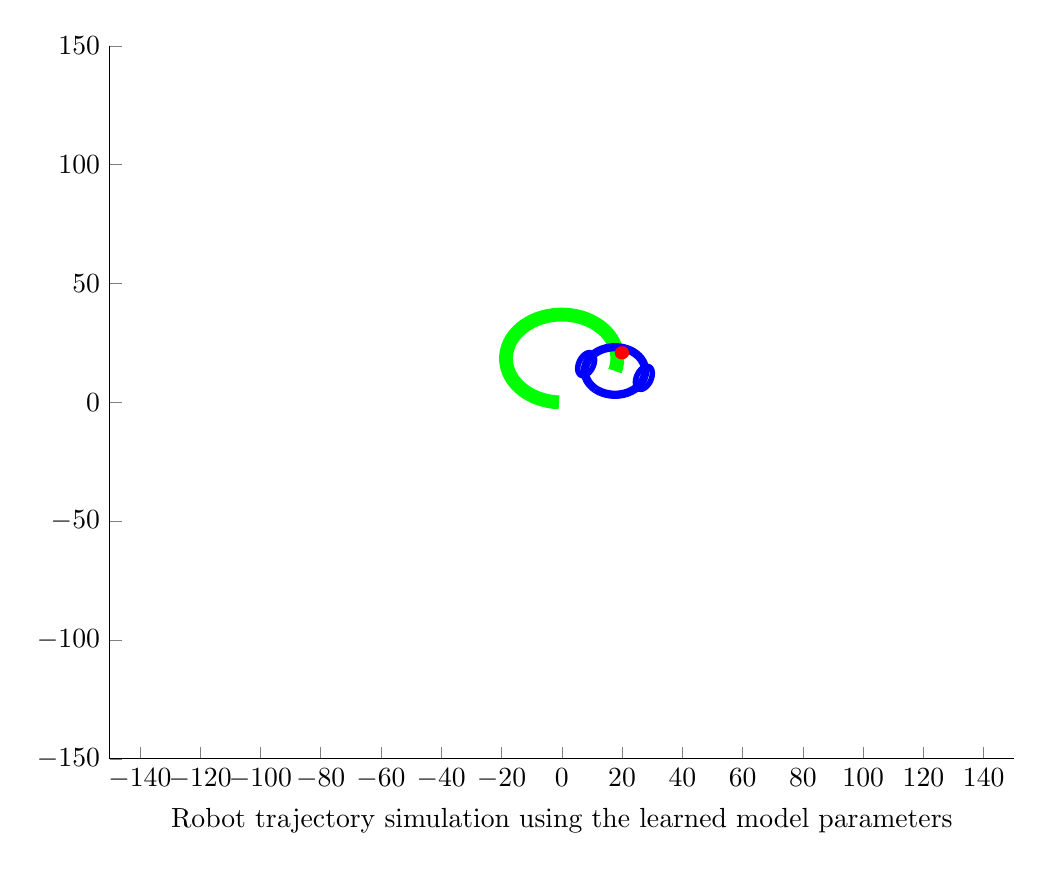
\begin{tikzpicture}

\begin{axis}[%
width=4.520833in,
height=3.565625in,
at={(0.758333in,0.48125in)},
scale only axis,
every outer x axis line/.append style={black},
every x tick label/.append style={font=\color{black}},
xmin=-150,
xmax=150,
xlabel={Robot trajectory simulation using the learned model parameters},
every outer y axis line/.append style={black},
every y tick label/.append style={font=\color{black}},
ymin=-150,
ymax=150,
axis x line*=bottom,
axis y line*=left
]
\addplot [color=green,solid,line width=5.0pt,forget plot]
  table[row sep=crcr]{%
-0.923637182339139	0.020930497956188\\
-1.84507127481466	0.0880344737541712\\
-2.76199547048803	0.201143932831737\\
-3.67211425293116	0.359975706064642\\
-4.57314914304352	0.564132158679502\\
-5.46284440321638	0.81310218573101\\
-6.3389726845638	1.10626249165134\\
-7.19934060308256	1.44287915066834\\
-8.04179423078115	1.8221094441861\\
-8.86422448803072	2.2430039705279\\
-9.66457242363837	2.70450902175989\\
-10.4408343694241	3.20546922164514\\
-11.1910669563967	3.74463041812388\\
-11.9133919799715	4.32064282307867\\
-12.6060011020481	4.93206439152413\\
-13.2671603781791	5.57736443176133\\
-13.8952145984929	6.25492743745899\\
-14.4885914315066	6.96305713206776\\
-15.0458053604515	7.69998071544249\\
-15.5654614022594	8.46385330204099\\
-16.0462585998973	9.25276253958834\\
-16.4869932793093	10.064733396644\\
-16.8865620628096	10.8977331070858\\
-17.2439646313848	11.7496762591329\\
-17.5583062289892	12.6184300161663\\
-17.8287999025631	13.5018194562778\\
-18.0547684721669	14.3976330171795\\
-18.2356462262988	15.3036280328414\\
-18.3709803381515	16.2175363479984\\
-18.4604319992624	17.1370699964684\\
-18.5037772677195	18.0599269290677\\
-18.500907628799	18.9837967767825\\
-18.4518302666315	19.9063666347698\\
-18.356668046217	20.8253268527063\\
-18.2156592058321	21.7383768169894\\
-18.0291567606018	22.6432307103154\\
-17.7976276187276	23.5376232342147\\
-17.5216514125838	24.4193152802186\\
-17.2019190476106	25.2860995354591\\
-16.8392309726344	26.1358060086686\\
-16.4344951759473	26.9663074627457\\
-15.9887249121616	27.7755247402852\\
-15.5030361655303	28.5614319687414\\
-14.9786448560849	29.3220616321929\\
-14.4168637955837	30.055509497011\\
-13.8190994008925	30.7599393791025\\
-13.1868481730247	31.4335877407897\\
-12.5216929506568	32.0747681058203\\
-11.8252989474971	32.6818752814551\\
-11.0994095834295	33.2533893770622\\
-10.3458421198677	33.7878796091574\\
-9.56648311024826	34.2840078833658\\
-8.76328367705033	34.7405321443362\\
-7.93825462716795	35.1563094852223\\
-7.09346141786205	35.5302990089454\\
-6.23101898589559	35.8615644340774\\
-5.35308645279707	36.1492764388171\\
-4.46186171950748	36.3927147371946\\
-3.55957596394319	36.5912698823051\\
-2.64848805525011	36.7444447920565\\
-1.73087889873284	36.8518559936128\\
-0.809045725616504	36.9132345834169\\
0.114703658063437	36.9284269003899\\
1.03805664904525	36.8973949106208\\
1.95870163643488	36.8202163025845\\
2.87433378881556	36.6970842926489\\
3.78266082438494	36.5283071413581\\
4.68140874967434	36.3143073817038\\
5.56832755248324	36.0556207613152\\
6.44119683477674	35.7528949012165\\
7.29783137144404	35.4068876745103\\
8.13608658100167	35.0184653090451\\
8.9538638945455	34.5886002188167\\
9.74911600951048	34.1183685695333\\
10.5198520150853	33.6089475844387\\
11.2641423764502	33.0616125971381\\
11.9801237653608	32.4777338588048\\
12.6660037249835	31.8587731077616\\
13.3200651573048	31.2062799100239\\
13.9406706218797	30.5218877799669\\
14.5262664351583	29.8073100908284\\
15.075386560127	29.0643357852845\\
15.5866562765267	28.2948248968387\\
16.0587956224601	27.5007038932342\\
16.4906225987716	26.6839608535493\\
16.8810561281782	25.8466404910481\\
17.2291187617424	24.9908390342485\\
17.5339391259122	24.1186989790214\\
17.7947541040015	23.2324037248604\\
18.0109107466501	22.3341721087485\\
18.1818679064801	21.4262528503081\\
18.3071975928564	20.5109189221393\\
18.3865860433596	19.5904618594412\\
18.4198345092891	18.6671860231618\\
18.4068597532301	17.7434028310387\\
18.3476942574378	16.8214249709728\\
18.2424861425181	15.9035606112228\\
18.0914987966086	14.9921076219144\\
17.8951102159871	14.0893478223301\\
17.6538120587593	13.1975412683832\\
};
\addplot [color=blue,solid,line width=3.0pt,forget plot]
  table[row sep=crcr]{%
27.6538120587593	13.1975412683832\\
27.6538070587598	13.2075412667165\\
27.653792058766	13.2175412550499\\
27.6537670587931	13.2275412233832\\
27.653732058866	13.2375411617166\\
27.6536870590198	13.2475410600501\\
27.6536320592993	13.2575409083839\\
27.6535670597598	13.2675406967179\\
27.653492060466	13.2775404150526\\
27.6534070614931	13.2875400533881\\
27.653312062926	13.2975396017249\\
27.6532070648597	13.3075390500633\\
27.6530920673993	13.3175383884039\\
27.6529670706597	13.3275376067475\\
27.6528320747659	13.3375366950947\\
27.6526870798529	13.3475356434465\\
27.6525320860658	13.3575344418039\\
27.6523670935594	13.3675330801682\\
27.6521921024989	13.3775315485407\\
27.6520071130591	13.3875298369229\\
27.6518121254251	13.3975279353165\\
27.6516071397919	13.4075258337235\\
27.6513921563644	13.417523522146\\
27.6511671753577	13.4275209905862\\
27.6509321969967	13.4375182290468\\
27.6506872215164	13.4475152275303\\
27.6504322491617	13.45751197604\\
27.6501672801877	13.4675084645789\\
27.6498923148593	13.4775046831507\\
27.6496073534515	13.4875006217591\\
27.6493123962492	13.4974962704082\\
27.6490074435474	13.5074916191023\\
27.6486924956511	13.517486657846\\
27.6483675528752	13.5274813766444\\
27.6480326155445	13.5374757655027\\
27.6476876839942	13.5474698144266\\
27.6473327585691	13.5574635134219\\
27.6469678396241	13.567456852495\\
27.6465929275242	13.5774498216526\\
27.6462080226442	13.5874424109016\\
27.6458131253691	13.5974346102496\\
27.6454082360938	13.6074264097042\\
27.6449933552231	13.6174177992737\\
27.644568483172	13.6274087689667\\
27.6441336203652	13.6373993087923\\
27.6436887672378	13.6473894087598\\
27.6432339242344	13.6573790588793\\
27.64276909181	13.667368249161\\
27.6422942704295	13.6773569696157\\
27.6418094605675	13.6873452102548\\
27.641314662709	13.69733296109\\
27.6408098773487	13.7073202121335\\
27.6402951049914	13.7173069533982\\
27.6397703461519	13.7272931748972\\
27.639235601355	13.7372788666443\\
27.6386908711353	13.7472640186539\\
27.6381361560377	13.7572486209408\\
27.6375714566168	13.7672326635203\\
27.6369967734373	13.7772161364086\\
27.6364121070739	13.787199029622\\
27.6358174581114	13.7971813331777\\
27.6352128271442	13.8071630370933\\
27.6345982147772	13.8171441313873\\
27.6339736216248	13.8271246060784\\
27.6333390483116	13.8371044511863\\
27.6326944954723	13.847083656731\\
27.6320399637515	13.8570622127334\\
27.6313754538035	13.8670401092149\\
27.630700966293	13.8770173361977\\
27.6300165018944	13.8869938837044\\
27.6293220612921	13.8969697417585\\
27.6286176451807	13.9069449003843\\
27.6279032542646	13.9169193496064\\
27.6271788892581	13.9268930794506\\
27.6264445508856	13.936866079943\\
27.6257002398814	13.9468383411106\\
27.6249459569899	13.9568098529813\\
27.6241817029653	13.9667806055834\\
27.6234074785719	13.9767505889462\\
27.6226232845839	13.9867197930998\\
27.6218291217855	13.9966882080749\\
27.6210249909709	14.0066558239032\\
27.6202108929442	14.016622630617\\
27.6193868285195	14.0265886182494\\
27.6185527985208	14.0365537768346\\
27.6177088037822	14.0465180964074\\
27.6168548451478	14.0564815670034\\
27.6159909234713	14.0664441786591\\
27.6151170396168	14.0764059214121\\
27.6142331944582	14.0863667853004\\
27.6133393888793	14.0963267603633\\
27.6124356237738	14.1062858366408\\
27.6115219000457	14.1162440041738\\
27.6105982186085	14.1262012530041\\
27.609664580386	14.1361575731746\\
27.6087209863118	14.1461129547288\\
27.6077674373295	14.1560673877114\\
27.6068039343926	14.1660208621679\\
27.6058304784647	14.175973368145\\
27.6048470705193	14.18592489569\\
27.6038537115396	14.1958754348515\\
27.6028504025191	14.2058249756789\\
27.6018371444611	14.2157735082227\\
27.6008139383788	14.2257210225343\\
27.5997807852955	14.2356675086662\\
27.5987376862443	14.245612956672\\
27.5976846422683	14.2555573566062\\
27.5966216544205	14.2655006985244\\
27.595548723764	14.2754429724833\\
27.5944658513716	14.2853841685405\\
27.5933730383263	14.295324276755\\
27.5922702857208	14.3052632871865\\
27.5911575946579	14.3152011898961\\
27.5900349662504	14.3251379749458\\
27.5889024016207	14.335073632399\\
27.5877599019015	14.3450081523198\\
27.5866074682353	14.3549415247739\\
27.5854451017745	14.3648737398279\\
27.5842728036815	14.3748047875494\\
27.5830905751286	14.3847346580076\\
27.581898417298	14.3946633412724\\
27.5806963313819	14.4045908274153\\
27.5794843185823	14.4145171065087\\
27.5782623801113	14.4244421686264\\
27.5770305171908	14.4343660038432\\
27.5757887310526	14.4442886022355\\
27.5745370229386	14.4542099538805\\
27.5732753941005	14.4641300488569\\
27.5720038457999	14.4740488772447\\
27.5707223793083	14.483966429125\\
27.5694309959072	14.4938826945802\\
27.568129696888	14.503797663694\\
27.566818483552	14.5137113265516\\
27.5654973572104	14.5236236732393\\
27.5641663191843	14.5335346938446\\
27.5628253708048	14.5434443784567\\
27.5614745134128	14.5533527171657\\
27.5601137483592	14.5632597000634\\
27.5587430770047	14.5731653172428\\
27.55736250072	14.5830695587983\\
27.5559720208857	14.5929724148256\\
27.5545716388923	14.6028738754218\\
27.5531613561401	14.6127739306856\\
27.5517411740394	14.6226725707168\\
27.5503110940105	14.6325697856168\\
27.5488711174833	14.6424655654885\\
27.5474212458979	14.6523599004359\\
27.5459614807041	14.6622527805649\\
27.5444918233618	14.6721441959824\\
27.5430122753405	14.6820341367972\\
27.5415228381198	14.6919225931192\\
27.5400235131891	14.70180955506\\
27.5385143020478	14.7116950127327\\
27.5369952062051	14.7215789562517\\
27.5354662271801	14.7314613757332\\
27.5339273665017	14.7413422612946\\
27.5323786257089	14.7512216030553\\
27.5308200063503	14.7610993911357\\
27.5292515099846	14.7709756156581\\
27.5276731381802	14.7808502667463\\
27.5260848925156	14.7907233345257\\
27.524486774579	14.8005948091231\\
27.5228787859685	14.8104646806671\\
27.5212609282921	14.8203329392878\\
27.5196332031676	14.830199575117\\
27.5179956122228	14.840064578288\\
27.5163481570953	14.8499279389359\\
27.5146908394325	14.8597896471972\\
27.5130236608918	14.8696496932103\\
27.5113466231402	14.879508067115\\
27.5096597278549	14.8893647590532\\
27.5079629767228	14.8992197591679\\
27.5062563714406	14.9090730576044\\
27.5045399137149	14.9189246445092\\
27.5028136052621	14.9287745100307\\
27.5010774478087	14.9386226443192\\
27.4993314430906	14.9484690375264\\
27.497575592854	14.958313679806\\
27.4958098988547	14.9681565613133\\
27.4940343628584	14.9779976722055\\
27.4922489866406	14.9878370026415\\
27.4904537719866	14.9976745427818\\
27.4886487206918	15.007510282789\\
27.4868338345611	15.0173442128274\\
27.4850091154095	15.027176323063\\
27.4831745650617	15.0370066036636\\
27.4813301853521	15.0468350447991\\
27.4794759781253	15.056661636641\\
27.4776119452353	15.0664863693626\\
27.4757380885463	15.0763092331393\\
27.473854409932	15.0861302181482\\
27.4719609112763	15.0959493145683\\
27.4700575944725	15.1057665125805\\
27.468144461424	15.1155818023677\\
27.4662215140438	15.1253951741144\\
27.4642887542551	15.1352066180074\\
27.4623461839905	15.1450161242353\\
27.4603938051926	15.1548236829884\\
27.4584316198137	15.1646292844593\\
27.4564596298161	15.1744329188423\\
27.4544778371718	15.1842345763338\\
27.4524862438624	15.1940342471322\\
27.4504848518798	15.2038319214378\\
27.4484736632251	15.2136275894529\\
27.4464526799096	15.2234212413818\\
27.4444219039544	15.233212867431\\
27.4423813373901	15.2430024578087\\
27.4403309822574	15.2527900027254\\
27.4382708406065	15.2625754923935\\
27.4362009144977	15.2723589170276\\
27.4341212060008	15.2821402668442\\
27.4320317171956	15.291919532062\\
27.4299324501716	15.3016967029017\\
27.427823407028	15.3114717695861\\
27.4257045898738	15.3212447223402\\
27.423576000828	15.331015551391\\
27.421437642019	15.3407842469678\\
27.4192895155852	15.3505507993017\\
27.4171316236748	15.3603151986262\\
27.4149639684456	15.3700774351771\\
27.4127865520654	15.3798374991919\\
27.4105993767115	15.3895953809107\\
27.408402444571	15.3993510705755\\
27.406195757841	15.4091045584308\\
27.4039793187281	15.4188558347229\\
27.4017531294488	15.4286048897007\\
27.3995171922292	15.438351713615\\
27.3972715093052	15.448096296719\\
27.3950160829227	15.4578386292682\\
27.3927509153369	15.4675787015203\\
27.3904760088131	15.4773165037351\\
27.3881913656261	15.4870520261748\\
27.3858969880607	15.496785259104\\
27.3835928784111	15.5065161927894\\
27.3812790389815	15.5162448175001\\
27.3789554720858	15.5259711235074\\
27.3766221800474	15.535695101085\\
27.3742791651997	15.545416740509\\
27.3719264298858	15.5551360320577\\
27.3695639764583	15.5648529660119\\
27.3671918072796	15.5745675326546\\
27.3648099247221	15.5842797222711\\
27.3624183311674	15.5939895251495\\
27.3600170290073	15.6036969315798\\
27.3576060206431	15.6134019318546\\
27.3551853084857	15.6231045162689\\
27.3527548949558	15.6328046751202\\
27.350314782484	15.6425023987083\\
27.3478649735102	15.6521976773355\\
27.3454054704843	15.6618905013065\\
27.3429362758658	15.6715808609284\\
27.3404573921239	15.681268746511\\
27.3379688217374	15.6909541483663\\
27.335470567195	15.7006370568089\\
27.3329626309949	15.7103174621559\\
27.3304450156451	15.719995354727\\
27.3279177236631	15.7296707248442\\
27.3253807575762	15.7393435628321\\
27.3228341199215	15.7490138590179\\
27.3202778132454	15.7586816037314\\
27.3177118401045	15.7683467873048\\
27.3151362030645	15.7780094000728\\
27.3125509047012	15.7876694323729\\
27.3099559475999	15.7973268745451\\
27.3073513343555	15.8069817169319\\
27.3047370675726	15.8166339498785\\
27.3021131498656	15.8262835637325\\
27.2994795838582	15.8359305488446\\
27.2968363721841	15.8455748955675\\
27.2941835174865	15.8552165942571\\
27.2915210224182	15.8648556352715\\
27.2888488896418	15.8744920089718\\
27.2861671218294	15.8841257057216\\
27.2834757216627	15.8937567158872\\
27.2807746918331	15.9033850298375\\
27.2780640350417	15.9130106379443\\
27.2753437539991	15.922633530582\\
27.2726138514257	15.9322536981276\\
27.2698743300512	15.9418711309611\\
27.2671251926153	15.9514858194649\\
27.264366441867	15.9610977540243\\
27.2615980805652	15.9707069250276\\
27.2588201114781	15.9803133228654\\
27.2560325373838	15.9899169379313\\
27.2532353610698	15.9995177606219\\
27.2504285853333	16.0091157813361\\
27.2476122129811	16.0187109904761\\
27.2447862468295	16.0283033784467\\
27.2419506897046	16.0378929356553\\
27.2391055444418	16.0474796525125\\
27.2362508138863	16.0570635194316\\
27.2333865008929	16.0666445268286\\
27.2305126083258	16.0762226651226\\
27.2276291390589	16.0857979247355\\
27.2247360959758	16.095370296092\\
27.2218334819695	16.1049397696196\\
27.2189212999425	16.114506335749\\
27.2159995528071	16.1240699849136\\
27.2130682434849	16.1336307075497\\
27.2101273749074	16.1431884940967\\
27.2071769500154	16.1527433349966\\
27.2042169717593	16.1622952206947\\
27.201247443099	16.1718441416391\\
27.1982683670042	16.1813900882809\\
27.1952797464538	16.1909330510741\\
27.1922815844366	16.2004730204758\\
27.1892738839506	16.210009986946\\
27.1862566480036	16.2195439409477\\
27.1832298796128	16.229074872947\\
27.180193581805	16.238602773413\\
27.1771477576165	16.2481276328176\\
27.174092410093	16.2576494416362\\
27.17102754229	16.2671681903469\\
27.1679531572723	16.2766838694309\\
27.1648692581143	16.2861964693725\\
27.1617758478999	16.2957059806592\\
27.1586729297225	16.3052123937815\\
27.155560506685	16.3147156992329\\
27.1524385818998	16.3242158875101\\
27.1493071584889	16.333712949113\\
27.1461662395837	16.3432068745444\\
27.1430158283252	16.3526976543105\\
27.1398559278636	16.3621852789205\\
27.136686541359	16.3716697388867\\
27.1335076719806	16.3811510247247\\
27.1303193229075	16.3906291269532\\
27.1271214973279	16.4001040360942\\
27.1239141984396	16.4095757426726\\
27.12069742945	16.4190442372168\\
27.1174711935758	16.4285095102583\\
27.1142354940432	16.4379715523319\\
27.110990334088	16.4474303539754\\
27.1077357169553	16.4568859057302\\
27.1044716458998	16.4663381981405\\
27.1011981241854	16.4757872217542\\
27.0979151550858	16.4852329671222\\
27.0946227418838	16.4946754247988\\
27.091320887872	16.5041145853416\\
27.0880095963521	16.5135504393112\\
27.0846888706355	16.522982977272\\
27.0813587140428	16.5324121897914\\
27.0780191299043	16.5418380674401\\
27.0746701215595	16.5512606007922\\
27.0713116923574	16.5606797804254\\
27.0679438456564	16.5700955969203\\
27.0645665848245	16.5795080408611\\
27.0611799132388	16.5889171028355\\
27.057783834286	16.5983227734343\\
27.0543783513623	16.6077250432519\\
27.050963467873	16.617123902886\\
27.0475391872331	16.6265193429377\\
27.0441055128669	16.6359113540117\\
27.040662448208	16.6452999267158\\
27.0372099966995	16.6546850516616\\
27.0337481617938	16.6640667194639\\
27.0302769469528	16.6734449207411\\
27.0267963556477	16.6828196461148\\
27.0233063913591	16.6921908862105\\
27.019807057577	16.7015586316569\\
27.0162983578006	16.7109228730861\\
27.0127802955387	16.7202836011341\\
27.0092528743093	16.72964080644\\
27.0057160976399	16.7389944796467\\
27.0021699690673	16.7483446114005\\
26.9986144921375	16.7576911923512\\
26.9950496704061	16.7670342131523\\
26.9914755074378	16.7763736644608\\
26.9878920068069	16.7857095369371\\
26.9842991720967	16.7950418212455\\
26.9806970069003	16.8043705080536\\
26.9770855148197	16.8136955880328\\
26.9734646994664	16.823017051858\\
26.9698345644612	16.8323348902077\\
26.9661951134343	16.8416490937641\\
26.9625463500252	16.8509596532129\\
26.9588882778825	16.8602665592437\\
26.9552209006644	16.8695698025495\\
26.9515442220382	16.878869373827\\
26.9478582456806	16.8881652637768\\
26.9441629752776	16.8974574631029\\
26.9404584145244	16.906745962513\\
26.9367445671257	16.9160307527188\\
26.9330214367953	16.9253118244355\\
26.9292890272562	16.9345891683818\\
26.9255473422409	16.9438627752806\\
26.9217963854912	16.9531326358582\\
26.9180361607579	16.9623987408448\\
26.9142666718012	16.9716610809741\\
26.9104879223907	16.980919646984\\
26.9066999163051	16.9901744296158\\
26.9029026573325	16.9994254196148\\
26.89909614927	17.00867260773\\
26.8952803959242	17.0179159847141\\
26.8914554011108	17.0271555413238\\
26.8876211686548	17.0363912683196\\
26.8837777023905	17.0456231564657\\
26.8799250061613	17.0548511965302\\
26.87606308382	17.0640753792851\\
26.8721919392284	17.0732956955062\\
26.8683115762577	17.0825121359732\\
26.8644219987882	17.0917246914697\\
26.8605232107095	17.1009333527831\\
26.8566152159205	17.1101381107047\\
26.8526980183291	17.1193389560298\\
26.8487716218525	17.1285358795576\\
26.8448360304171	17.137728872091\\
26.8408912479585	17.1469179244372\\
26.8369372784214	17.1561030274071\\
26.8329741257599	17.1652841718155\\
26.8290017939372	17.1744613484813\\
26.8250202869254	17.1836345482274\\
26.8210296087062	17.1928037618806\\
26.8170297632701	17.2019689802716\\
26.8130207546172	17.2111301942352\\
26.8090025867563	17.2202873946102\\
26.8049752637057	17.2294405722395\\
26.8009387894926	17.2385897179697\\
26.7968931681535	17.2477348226519\\
26.7928384037341	17.2568758771408\\
26.7887745002891	17.2660128722955\\
26.7847014618824	17.2751457989789\\
26.7806192925871	17.2842746480581\\
26.7765279964853	17.2933994104043\\
26.7724275776683	17.3025200768927\\
26.7683180402366	17.3116366384026\\
26.7641993882997	17.3207490858175\\
26.7600716259762	17.3298574100249\\
26.7559347573938	17.3389616019165\\
26.7517887866896	17.3480616523881\\
26.7476337180093	17.3571575523397\\
26.7434695555082	17.3662492926753\\
26.7392963033503	17.3753368643033\\
26.7351139657089	17.384420258136\\
26.7309225467664	17.3934994650901\\
26.7267220507142	17.4025744760863\\
26.7225124817527	17.4116452820497\\
26.7182938440916	17.4207118739094\\
26.7140661419494	17.4297742425989\\
26.7098293795539	17.4388323790557\\
26.7055835611418	17.4478862742218\\
26.701328690959	17.4569359190432\\
26.6970647732603	17.4659813044703\\
26.6927918123096	17.4750224214578\\
26.6885098123799	17.4840592609644\\
26.6842187777533	17.4930918139535\\
26.6799187127207	17.5021200713923\\
26.6756096215821	17.5111440242527\\
26.6712915086468	17.5201636635107\\
26.6669643782327	17.5291789801466\\
26.6626282346671	17.5381899651452\\
26.6582830822861	17.5471966094955\\
26.6539289254348	17.5561989041908\\
26.6495657684674	17.5651968402288\\
26.645193615747	17.5741904086116\\
26.6408124716458	17.5831796003457\\
26.6364223405449	17.5921644064417\\
26.6320232268346	17.601144817915\\
26.6276151349138	17.6101208257852\\
26.6231980691906	17.6190924210761\\
26.6187720340822	17.6280595948162\\
26.6143370340146	17.6370223380384\\
26.6098930734227	17.6459806417799\\
26.6054401567506	17.6549344970824\\
26.6009782884511	17.663883894992\\
26.5965074729862	17.6728288265594\\
26.5920277148265	17.6817692828396\\
26.587539018452	17.6907052548921\\
26.5830413883512	17.699636733781\\
26.5785348290219	17.7085637105749\\
26.5740193449705	17.7174861763466\\
26.5694949407126	17.7264041221739\\
26.5649616207726	17.7353175391387\\
26.5604193896837	17.7442264183275\\
26.5558682519882	17.7531307508316\\
26.5513082122373	17.7620305277466\\
26.546739274991	17.7709257401728\\
26.5421614448182	17.7798163792148\\
26.5375747262968	17.7887024359821\\
26.5329791240134	17.7975839015886\\
26.5283746425637	17.8064607671529\\
26.5237612865522	17.815333023798\\
26.5191390605921	17.8242006626518\\
26.5145079693059	17.8330636748466\\
26.5098680173244	17.8419220515193\\
26.5052192092877	17.8507757838117\\
26.5005615498446	17.8596248628699\\
26.4958950436528	17.868469279845\\
26.4912196953787	17.8773090258924\\
26.4865355096977	17.8861440921724\\
26.481842491294	17.89497446985\\
26.4771406448605	17.9038001500948\\
26.4724299750993	17.9126211240811\\
26.4677104867208	17.9214373829879\\
26.4629821844447	17.930248917999\\
26.4582450729992	17.9390557203029\\
26.4534991571214	17.9478577810927\\
26.4487444415572	17.9566550915664\\
26.4439809310614	17.9654476429267\\
26.4392086303974	17.974235426381\\
26.4344275443376	17.9830184331415\\
26.4296376776631	17.9917966544252\\
26.4248390351636	18.000570081454\\
26.4200316216379	18.0093387054544\\
26.4152154418934	18.0181025176577\\
26.4103905007462	18.0268615093002\\
26.4055568030213	18.0356156716228\\
26.4007143535524	18.0443649958714\\
26.395863157182	18.0531094732968\\
26.3910032187611	18.0618490951543\\
26.3861345431499	18.0705838527044\\
26.3812571352168	18.0793137372123\\
26.3763709998395	18.0880387399481\\
26.3714761419039	18.0967588521869\\
26.3665725663049	18.1054740652085\\
26.3616602779462	18.1141843702978\\
26.35673928174	18.1228897587443\\
26.3518095826073	18.1315902218428\\
26.3468711854778	18.1402857508927\\
26.3419240952898	18.1489763371985\\
26.3369683169906	18.1576619720697\\
26.3320038555358	18.1663426468206\\
26.32703071589	18.1750183527705\\
26.3220489030262	18.1836890812438\\
26.3170584219263	18.1923548235696\\
26.3120592775808	18.2010155710824\\
26.3070514749887	18.2096713151212\\
26.302035019158	18.2183220470304\\
26.297009915105	18.2269677581592\\
26.2919761678549	18.235608439862\\
26.2869337824414	18.244244083498\\
26.2818827639069	18.2528746804317\\
26.2768231173025	18.2615002220323\\
26.2717548476876	18.2701206996744\\
26.2666779601307	18.2787361047375\\
26.2615924597087	18.2873464286062\\
26.2564983515069	18.2959516626702\\
26.2513956406196	18.3045517983241\\
26.2462843321493	18.313146826968\\
26.2411644312076	18.3217367400068\\
26.2360359429142	18.3303215288505\\
26.2308988723976	18.3389011849143\\
26.2257532247949	18.3474756996187\\
26.2205990052517	18.3560450643891\\
26.2154362189224	18.3646092706561\\
26.2102648709696	18.3731683098556\\
26.2050849665646	18.3817221734284\\
26.1998965108875	18.3902708528207\\
26.1946995091267	18.3988143394839\\
26.1894939664791	18.4073526248745\\
26.1842798881503	18.4158857004542\\
26.1790572793544	18.4244135576898\\
26.173826145314	18.4329361880536\\
26.1685864912602	18.4414535830229\\
26.1633383224327	18.4499657340803\\
26.1580816440796	18.4584726327137\\
26.1528164614577	18.4669742704162\\
26.147542779832	18.4754706386861\\
26.1422606044764	18.4839617290271\\
26.1369699406729	18.4924475329481\\
26.1316707937122	18.5009280419632\\
26.1263631688935	18.509403247592\\
26.1210470715244	18.5178731413593\\
26.115722506921	18.5263377147952\\
26.1103894804078	18.534796959435\\
26.105047997318	18.5432508668196\\
26.0996980629929	18.551699428495\\
26.0943396827825	18.5601426360128\\
26.0889728620451	18.5685804809296\\
26.0835976061477	18.5770129548076\\
26.0782139204655	18.5854400492144\\
26.072821810382	18.5938617557229\\
26.0674212812895	18.6022780659113\\
26.0620123385885	18.6106889713634\\
26.056594987688	18.6190944636683\\
26.0511692340052	18.6274945344204\\
26.0457350829659	18.6358891752196\\
26.0402925400043	18.6442783776715\\
26.0348416105629	18.6526621333866\\
26.0293823000926	18.6610404339814\\
26.0239146140528	18.6694132710774\\
26.0184385579112	18.6777806363019\\
26.0129541371438	18.6861425212875\\
26.0074613572349	18.6944989176723\\
26.0019602236775	18.7028498170999\\
25.9964507419726	18.7111952112195\\
25.9909329176297	18.7195350916855\\
25.9854067561667	18.7278694501582\\
25.9798722631096	18.7361982783031\\
25.974329443993	18.7445215677915\\
25.9687783043598	18.7528393103001\\
25.963218849761	18.761151497511\\
25.9576510857561	18.7694581211123\\
25.9520750179128	18.7777591727971\\
25.9464906518073	18.7860546442645\\
25.9408979930239	18.794344527219\\
25.9352970471552	18.8026288133706\\
25.9296878198023	18.8109074944353\\
25.9240703165743	18.8191805621341\\
25.9184445430887	18.8274480081941\\
25.9128105049713	18.8357098243479\\
25.9071682078561	18.8439660023336\\
25.9015176573855	18.852216533895\\
25.89585885921	18.8604614107816\\
25.8901918189883	18.8687006247485\\
25.8845165423876	18.8769341675566\\
25.8788330350831	18.8851620309722\\
25.8731413027583	18.8933842067676\\
25.867441351105	18.9016006867204\\
25.861733185823	18.9098114626144\\
25.8560168126206	18.9180165262386\\
25.8502922372141	18.926215869388\\
25.8445594653282	18.9344094838633\\
25.8388185026955	18.9425973614709\\
25.833069355057	18.9507794940229\\
25.8273120281619	18.9589558733371\\
25.8215465277676	18.9671264912372\\
25.8157728596394	18.9752913395525\\
25.8099910295511	18.9834504101183\\
25.8042010432846	18.9916036947754\\
25.7984029066297	18.9997511853705\\
25.7925966253847	19.0078928737563\\
25.7867822053557	19.0160287517909\\
25.7809596523574	19.0241588113385\\
25.775128972212	19.032283044269\\
25.7692901707505	19.0404014424583\\
25.7634432538115	19.0485139977878\\
25.757588227242	19.0566207021452\\
25.751725096897	19.0647215474235\\
25.7458538686397	19.0728165255221\\
25.7399745483412	19.0809056283459\\
25.7340871418809	19.0889888478059\\
25.7281916551461	19.0970661758188\\
25.7222880940325	19.1051376043072\\
25.7163764644435	19.1132031251998\\
25.7104567722907	19.1212627304311\\
25.704529023494	19.1293164119413\\
25.6985932239809	19.137364161677\\
25.6926493796873	19.1454059715902\\
25.6866974965571	19.1534418336392\\
25.6807375805421	19.1614717397882\\
25.6747696376023	19.1694956820071\\
25.6687936737055	19.1775136522722\\
25.6628096948278	19.1855256425654\\
25.6568177069531	19.1935316448747\\
25.6508177160735	19.2015316511941\\
25.6448097281888	19.2095256535236\\
25.6387937493072	19.2175136438693\\
25.6327697854445	19.2254956142431\\
25.6267378426248	19.233471556663\\
25.6206979268799	19.2414414631531\\
25.6146500442499	19.2494053257436\\
25.6085942007825	19.2573631364705\\
25.6025304025337	19.2653148873761\\
25.5964586555671	19.2732605705085\\
25.5903789659546	19.2812001779221\\
25.5842913397759	19.2891337016774\\
25.5781957831186	19.2970611338407\\
25.5720923020782	19.3049824664846\\
25.5659809027582	19.3128976916879\\
25.55986159127	19.3208068015352\\
25.553734373733	19.3287097881175\\
25.5475992562743	19.3366066435319\\
25.541456245029	19.3444973598813\\
25.5353053461403	19.3523819292752\\
25.5291465657589	19.3602603438289\\
25.5229799100436	19.3681325956641\\
25.5168053851612	19.3759986769084\\
25.5106229972861	19.3838585796959\\
25.5044327526007	19.3917122961665\\
25.4982346572952	19.3995598184667\\
25.4920287175678	19.4074011387488\\
25.4858149396244	19.4152362491716\\
25.4795933296788	19.4230651418999\\
25.4733638939526	19.4308878091048\\
25.4671266386752	19.4387042429637\\
25.4608815700838	19.4465144356602\\
25.4546286944236	19.454318379384\\
25.4483680179474	19.4621160663313\\
25.4420995469159	19.4699074887042\\
25.4358232875975	19.4776926387115\\
25.4295392462686	19.4854715085679\\
25.4232474292131	19.4932440904946\\
25.416947842723	19.501010376719\\
25.4106404930976	19.5087703594748\\
25.4043253866445	19.5165240310021\\
25.3980025296787	19.5242713835471\\
25.3916719285231	19.5320124093625\\
25.3853335895083	19.5397471007073\\
25.3789875189725	19.5474754498468\\
25.372633723262	19.5551974490527\\
25.3662722087304	19.5629130906029\\
25.3599029817393	19.5706223667818\\
25.353526048658	19.5783252698802\\
25.3471414158633	19.586021792195\\
25.3407490897398	19.5937119260299\\
25.33434907668	19.6013956636947\\
25.3279413830838	19.6090729975056\\
25.321526015359	19.6167439197853\\
25.3151029799208	19.6244084228629\\
25.3086722831923	19.6320664990738\\
25.3022339316042	19.6397181407601\\
25.2957879315949	19.6473633402701\\
25.2893342896104	19.6550020899585\\
25.2828730121043	19.6626343821866\\
25.2764041055378	19.6702602093221\\
25.26992757638	19.6778795637393\\
25.2634434311072	19.6854924378187\\
25.2569516762037	19.6930988239474\\
25.2504523181613	19.7006987145192\\
25.2439453634792	19.708292101934\\
25.2374308186644	19.7158789785986\\
25.2309086902315	19.723459336926\\
25.2243789847026	19.7310331693358\\
25.2178417086075	19.7386004682543\\
25.2112968684832	19.7461612261142\\
25.2047444708749	19.7537154353546\\
25.1981845223347	19.7612630884214\\
25.1916170294227	19.768804177767\\
25.1850419987064	19.7763386958502\\
25.1784594367607	19.7838666351365\\
25.1718693501683	19.7913879880979\\
25.1652717455192	19.7989027472133\\
25.1586666294111	19.8064109049676\\
25.152054008449	19.8139124538529\\
25.1454338892456	19.8214073863676\\
25.138806278421	19.8288956950167\\
25.1321711826028	19.8363773723119\\
25.1255286084261	19.8438524107716\\
25.1188785625334	19.8513208029207\\
25.1122210515749	19.8587825412908\\
25.105556082208	19.8662376184202\\
25.0988836610978	19.8736860268538\\
25.0922037949165	19.8811277591432\\
25.0855164903441	19.8885628078466\\
25.0788217540679	19.8959911655291\\
25.0721195927826	19.9034128247622\\
25.0654100131904	19.9108277781244\\
25.0586930220009	19.9182360182006\\
25.051968625931	19.9256375375826\\
25.0452368317052	19.9330323288689\\
25.0384976460552	19.9404203846647\\
25.0317510757203	19.9478016975819\\
25.0249971274469	19.9551762602393\\
25.0182358079891	19.9625440652622\\
25.0114671241081	19.9699051052829\\
25.0046910825727	19.9772593729404\\
24.9979076901589	19.9846068608803\\
24.9911169536501	19.9919475617551\\
24.984318879837	19.9992814682243\\
24.9775134755177	20.0066085729538\\
24.9707007474975	20.0139288686165\\
24.9638807025893	20.0212423478923\\
24.9570533476131	20.0285490034675\\
24.9502186893962	20.0358488280356\\
24.9433767347732	20.0431418142967\\
24.9365274905862	20.0504279549578\\
24.9296709636844	20.0577072427327\\
24.9228071609242	20.0649796703423\\
24.9159360891696	20.0722452305141\\
24.9090577552915	20.0795039159824\\
24.9021721661684	20.0867557194887\\
24.8952793286857	20.0940006337811\\
24.8883792497364	20.1012386516148\\
24.8814719362205	20.1084697657516\\
24.8745573950453	20.1156939689605\\
24.8676356331254	20.1229112540172\\
24.8607066573825	20.1301216137046\\
24.8537704747456	20.1373250408122\\
24.8468270921509	20.1445215281366\\
24.8398765165418	20.1517110684813\\
24.8329187548688	20.1588936546568\\
24.8259538140897	20.1660692794805\\
24.8189817011694	20.1732379357767\\
24.8120024230801	20.1803996163769\\
24.805015986801	20.1875543141193\\
24.7980223993186	20.1947020218492\\
24.7910216676265	20.201842732419\\
24.7840137987253	20.2089764386879\\
24.776998799623	20.2161031335222\\
24.7699766773346	20.2232228097952\\
24.7629474388821	20.2303354603873\\
24.7559110912948	20.2374410781858\\
24.7488676416091	20.244539656085\\
24.7418170968684	20.2516311869865\\
24.7347594641233	20.2587156637986\\
24.7276947504313	20.2657930794369\\
24.7206229628573	20.2728634268239\\
24.7135441084729	20.2799266988895\\
24.7064581943571	20.2869828885701\\
24.6993652275957	20.2940319888098\\
24.6922652152817	20.3010739925593\\
24.6851581645152	20.3081088927767\\
24.6780440824031	20.315136682427\\
24.6709229760596	20.3221573544825\\
24.6637948526058	20.3291709019226\\
24.6566597191697	20.3361773177336\\
24.6495175828866	20.3431765949091\\
24.6423684508986	20.3501687264499\\
24.6352123303547	20.3571537053639\\
24.6280492284111	20.364131524666\\
24.620879152231	20.3711021773784\\
24.6137021089843	20.3780656565306\\
24.6065181058482	20.3850219551589\\
24.5993271500066	20.3919710663072\\
24.5921292486505	20.3989129830262\\
24.5849244089778	20.4058476983742\\
24.5777126381933	20.4127752054163\\
24.5704939435088	20.4196954972251\\
24.563268332143	20.4266085668803\\
24.5560358113215	20.4335144074687\\
24.5487963882768	20.4404130120846\\
24.5415500702484	20.4473043738294\\
24.5342968644825	20.4541884858117\\
24.5270367782324	20.4610653411474\\
24.5197698187581	20.4679349329596\\
24.5124959933267	20.4747972543787\\
24.5052153092119	20.4816522985425\\
24.4979277736944	20.4885000585958\\
24.4906333940618	20.495340527691\\
24.4833321776084	20.5021736989875\\
24.4760241316355	20.5089995656522\\
24.468709263451	20.5158181208592\\
24.4613875803699	20.5226293577899\\
24.4540590897139	20.5294332696332\\
24.4467237988114	20.5362298495851\\
24.4393817149977	20.543019090849\\
24.432032845615	20.5498009866357\\
24.424677198012	20.5565755301633\\
24.4173147795444	20.5633427146572\\
24.4099455975747	20.5701025333504\\
24.402569659472	20.5768549794828\\
24.3951869726123	20.5836000463022\\
24.3877975443782	20.5903377270634\\
24.3804013821592	20.5970680150288\\
24.3729984933514	20.603790903468\\
24.3655888853578	20.6105063856582\\
24.3581725655878	20.617214454884\\
24.350749541458	20.6239151044371\\
24.3433198203912	20.630608327617\\
24.3358834098172	20.6372941177305\\
24.3284403171724	20.6439724680918\\
24.3209905498999	20.6506433720225\\
24.3135341154495	20.6573068228517\\
24.3060710212776	20.663962813916\\
24.2986012748472	20.6706113385593\\
24.2911248836283	20.6772523901332\\
24.283641855097	20.6838859619966\\
24.2761521967365	20.6905120475159\\
24.2686559160364	20.6971306400651\\
24.261153020493	20.7037417330255\\
24.2536435176092	20.7103453197861\\
24.2461274148944	20.7169413937433\\
24.2386047198649	20.723529948301\\
24.2310754400433	20.7301109768706\\
24.2235395829588	20.7366844728711\\
24.2159971561473	20.7432504297291\\
24.2084481671513	20.7498088408785\\
24.2008926235198	20.756359699761\\
24.1933305328082	20.7629029998257\\
24.1857619025787	20.7694387345292\\
24.1781867403999	20.775966897336\\
24.1706050538469	20.7824874817177\\
24.1630168505015	20.7890004811539\\
24.1554221379518	20.7955058891315\\
24.1478209237927	20.8020036991451\\
24.1402132156251	20.8084939046969\\
24.132599021057	20.8149764992967\\
24.1249783477025	20.8214514764619\\
24.1173512031822	20.8279188297175\\
24.1097175951233	20.8343785525962\\
24.1020775311593	20.8408306386383\\
24.0944310189305	20.8472750813916\\
24.0867780660832	20.8537118744117\\
24.0791186802705	20.8601410112619\\
24.0714528691517	20.866562485513\\
24.0637806403926	20.8729762907435\\
24.0561020016654	20.8793824205396\\
24.0484169606489	20.8857808684952\\
24.040725525028	20.8921716282118\\
24.0330277024941	20.8985546932988\\
24.0253235007451	20.9049300573729\\
24.0176129274853	20.9112977140589\\
24.009895990425	20.9176576569891\\
24.0021726972814	20.9240098798035\\
23.9944430557777	20.93035437615\\
23.9867070736435	20.936691139684\\
23.9789647586148	20.9430201640688\\
23.9712161184339	20.9493414429754\\
23.9634611608496	20.9556549700824\\
23.9556998936166	20.9619607390763\\
23.9479323244963	20.9682587436514\\
23.9401584612563	20.9745489775097\\
23.9323783116704	20.980831434361\\
23.9245918835188	20.9871061079227\\
23.9167991845878	20.9933729919203\\
23.9090002226703	20.9996320800867\\
23.9011950055651	21.005883366163\\
23.8933835410775	21.0121268438979\\
23.885565837019	21.0183625070478\\
23.8777419012071	21.0245903493771\\
23.869911741466	21.030810364658\\
23.8620753656257	21.0370225466705\\
23.8542327815226	21.0432268892024\\
23.8463839969993	21.0494233860492\\
23.8385290199045	21.0556120310146\\
23.8306678580933	21.06179281791\\
23.8228005194269	21.0679657405544\\
23.8149270117725	21.074130792775\\
23.8070473430036	21.0802879684067\\
23.799161521	21.0864372612924\\
23.7912695536475	21.0925786652827\\
23.7833714488379	21.0987121742363\\
23.7754672144695	21.1048377820197\\
23.7675568584464	21.1109554825072\\
23.759640388679	21.1170652695811\\
23.7517178130838	21.1231671371318\\
23.7437891395834	21.1292610790572\\
23.7358543761064	21.1353470892634\\
23.7279135305876	21.1414251616645\\
23.7199666109678	21.1474952901824\\
23.712013625194	21.1535574687469\\
23.7040545812191	21.1596116912958\\
23.6960894870022	21.165657951775\\
23.6881183505083	21.1716962441382\\
23.6801411797087	21.1777265623471\\
23.6721579825805	21.1837489003713\\
23.6641687671068	21.1897632521886\\
23.6561735412769	21.1957696117846\\
23.6481723130861	21.2017679731529\\
23.6401650905355	21.2077583302951\\
23.6321518816323	21.213740677221\\
23.6241326943899	21.2197150079481\\
23.6161075368272	21.2256813165021\\
23.6080764169697	21.2316395969168\\
23.6000393428482	21.2375898432338\\
23.5919963225	21.2435320495029\\
23.583947363968	21.2494662097819\\
23.5758924753012	21.2553923181366\\
23.5678316645544	21.2613103686409\\
23.5597649397886	21.2672203553769\\
23.5516923090703	21.2731222724344\\
23.5436137804723	21.2790161139115\\
23.5355293620731	21.2849018739145\\
23.527439061957	21.2907795465576\\
23.5193428882145	21.296649125963\\
23.5112408489416	21.3025106062613\\
23.5031329522404	21.3083639815909\\
23.4950192062188	21.3142092460985\\
23.4868996189905	21.3200463939388\\
23.4787741986752	21.3258754192746\\
23.4706429533982	21.3316963162769\\
23.4625058912908	21.3375090791249\\
23.45436302049	21.3433137020058\\
23.4462143491388	21.3491101791149\\
23.4380598853857	21.3548985046557\\
23.4298996373854	21.36067867284\\
23.4217336132979	21.3664506778876\\
23.4135618212893	21.3722145140265\\
23.4053842695315	21.3779701754928\\
23.3972009662019	21.3837176565308\\
23.3890119194839	21.3894569513932\\
23.3808171375665	21.3951880543405\\
23.3726166286445	21.4009109596418\\
23.3644104009185	21.4066256615741\\
23.3561984625945	21.4123321544226\\
23.3479808218846	21.4180304324809\\
23.3397574870065	21.4237204900508\\
23.3315284661834	21.4294023214421\\
23.3232937676443	21.4350759209731\\
23.315053399624	21.44074128297\\
23.3068073703629	21.4463984017677\\
23.2985556881069	21.4520472717089\\
23.2902983611077	21.4576878871448\\
23.2820353976227	21.4633202424348\\
23.2737668059149	21.4689443319465\\
23.2654925942527	21.4745601500558\\
23.2572127709105	21.4801676911469\\
23.2489273441681	21.4857669496123\\
23.2406363223108	21.4913579198527\\
23.2323397136298	21.4969405962771\\
23.2240375264215	21.5025149733029\\
23.2157297689883	21.5080810453557\\
23.2074164496377	21.5136388068694\\
23.1990975766833	21.5191882522863\\
23.1907731584438	21.5247293760568\\
23.1824432032437	21.53026217264\\
23.1741077194129	21.5357866365029\\
23.1657667152869	21.5413027621212\\
23.1574201992067	21.5468105439786\\
23.1490681795188	21.5523099765675\\
23.1407106645752	21.5578010543884\\
23.1323476627335	21.5632837719502\\
23.1239791823567	21.5687581237702\\
23.1156052318131	21.574224104374\\
23.1072258194769	21.5796817082957\\
23.0988409537274	21.5851309300776\\
23.0904506429494	21.5905717642706\\
23.0820548955333	21.5960042054338\\
23.0736537198748	21.6014282481348\\
23.0652471243751	21.6068438869494\\
23.0568351174407	21.6122511164622\\
23.0484177074838	21.6176499312658\\
23.0399949029217	21.6230403259614\\
23.0315667121771	21.6284222951587\\
23.0231331436784	21.6337958334757\\
23.014694205859	21.6391609355388\\
23.006249907158	21.6445175959829\\
22.9978002560195	21.6498658094514\\
22.9893452608933	21.6552055705961\\
22.9808849302343	21.6605368740772\\
22.9724192725029	21.6658597145634\\
22.9639482961647	21.6711740867318\\
22.9554720096907	21.6764799852681\\
22.9469904215573	21.6817774048664\\
22.9385035402458	21.6870663402293\\
22.9300113742434	21.6923467860679\\
22.9215139320421	21.6976187371016\\
22.9130112221393	21.7028821880585\\
22.9045032530378	21.7081371336753\\
22.8959900332456	21.7133835686968\\
22.8874715712758	21.7186214878768\\
22.878947875647	21.7238508859773\\
22.8704189548827	21.7290717577689\\
22.861884817512	21.7342840980307\\
22.853345472069	21.7394879015504\\
22.844800927093	21.7446831631241\\
22.8362511911286	21.7498698775567\\
22.8276962727255	21.7550480396614\\
22.8191361804385	21.76021764426\\
22.8105709228279	21.765378686183\\
22.8020005084589	21.7705311602692\\
22.7934249459018	21.7756750613663\\
22.7848442437323	21.7808103843303\\
22.776258410531	21.7859371240259\\
22.7676674548838	21.7910552753264\\
22.7590713853816	21.7961648331136\\
22.7504702106206	21.8012657922779\\
22.7418639392018	21.8063581477184\\
22.7332525797315	21.8114418943427\\
22.7246361408211	21.8165170270672\\
22.7160146310871	21.8215835408166\\
22.707388059151	21.8266414305244\\
22.6987564336392	21.8316906911328\\
22.6901197631835	21.8367313175926\\
22.6814780564205	21.8417633048629\\
22.672831321992	21.846786647912\\
22.6641795685445	21.8518013417164\\
22.65552280473	21.8568073812614\\
22.6468610392052	21.8618047615411\\
22.6381942806318	21.866793477558\\
22.6295225376766	21.8717735243234\\
22.6208458190113	21.8767448968572\\
22.6121641333127	21.8817075901882\\
22.6034774892625	21.8866615993536\\
22.5947858955472	21.8916069193993\\
22.5860893608584	21.8965435453802\\
22.5773878938928	21.9014714723594\\
22.5686815033518	21.9063906954092\\
22.5599701979417	21.9113012096103\\
22.5512539863739	21.9162030100522\\
22.5425328773646	21.9210960918331\\
22.5338068796349	21.9259804500598\\
22.5250760019107	21.9308560798482\\
22.5163402529231	21.9357229763224\\
22.5075996414076	21.9405811346156\\
22.4988541761049	21.9454305498698\\
22.4901038657606	21.9502712172353\\
22.4813487191248	21.9551031318717\\
22.4725887449528	21.9599262889469\\
22.4638239520045	21.9647406836378\\
22.4550543490447	21.96954631113\\
22.446279944843	21.9743431666179\\
22.4375007481738	21.9791312453047\\
22.4287167678163	21.9839105424022\\
22.4199280125546	21.9886810531312\\
22.4111344911772	21.9934427727211\\
22.4023362124778	21.9981956964102\\
22.3935331852547	22.0029398194457\\
22.3847254183109	22.0076751370833\\
22.375912920454	22.0124016445878\\
22.3670957004967	22.0171193372327\\
22.3582737672562	22.0218282103002\\
22.3494471295543	22.0265282590815\\
22.3406157962178	22.0312194788766\\
22.3317797760779	22.0359018649942\\
22.3229390779707	22.0405754127519\\
22.3140937107368	22.0452401174762\\
22.3052436832217	22.0498959745024\\
22.2963890042754	22.0545429791747\\
22.2875296827525	22.0591811268459\\
22.2786657275123	22.0638104128781\\
22.2697971474189	22.0684308326418\\
22.2609239513408	22.0730423815167\\
22.2520461481512	22.0776450548913\\
22.2431637467278	22.0822388481628\\
22.2342767559532	22.0868237567374\\
22.2253851847142	22.0913997760303\\
22.2164890419025	22.0959669014655\\
22.2075883364142	22.1005251284757\\
22.19868307715	22.1050744525029\\
22.1897732730151	22.1096148689976\\
22.1808589329194	22.1141463734194\\
22.1719400657772	22.1186689612369\\
22.1630166805074	22.1231826279274\\
22.1540887860334	22.1276873689773\\
22.145156391283	22.1321831798818\\
22.1362195051886	22.1366700561452\\
22.1272781366871	22.1411479932806\\
22.11833229472	22.1456169868099\\
22.109381988233	22.1500770322643\\
22.1004272261764	22.1545281251837\\
22.091468017505	22.1589702611169\\
22.0825043711781	22.163403435622\\
22.0735362961592	22.1678276442656\\
22.0645638014164	22.1722428826235\\
22.0555868959223	22.1766491462806\\
22.0466055886536	22.1810464308306\\
22.0376198885919	22.1854347318761\\
22.0286298047226	22.189814045029\\
22.019635346036	22.1941843659098\\
22.0106365215265	22.1985456901483\\
22.0016333401928	22.2028980133831\\
21.9926258110382	22.2072413312619\\
21.9836139430703	22.2115756394413\\
21.9745977453008	22.2159009335872\\
21.965577226746	22.2202172093742\\
21.9565523964264	22.2245244624859\\
21.9475232633668	22.2288226886152\\
21.9384898365963	22.2331118834639\\
21.9294521251485	22.2373920427427\\
21.9204101380609	22.2416631621715\\
21.9113638843756	22.2459252374791\\
21.9023133731388	22.2501782644035\\
21.8932586134011	22.2544222386917\\
21.8841996142172	22.2586571560997\\
21.8751363846461	22.2628830123925\\
21.8660689337509	22.2670998033443\\
21.8569972705993	22.2713075247384\\
21.8479214042628	22.2755061723669\\
21.8388413438173	22.2796957420313\\
21.8297570983429	22.283876229542\\
21.8206686769238	22.2880476307185\\
21.8115760886484	22.2922099413894\\
21.8024793426093	22.2963631573924\\
21.7933784479033	22.3005072745742\\
21.7842734136313	22.3046422887908\\
21.7751642488982	22.3087681959072\\
21.7660509628133	22.3128849917973\\
21.7569335644898	22.3169926723445\\
21.7478120630452	22.3210912334411\\
21.7386864676009	22.3251806709884\\
21.7295567872825	22.3292609808971\\
21.7204230312198	22.3333321590869\\
21.7112852085464	22.3373942014865\\
21.7021433284002	22.341447104034\\
21.6929973999231	22.3454908626764\\
21.6838474322609	22.3495254733699\\
21.6746934345638	22.35355093208\\
21.6655354159855	22.3575672347812\\
21.6563733856843	22.3615743774572\\
21.6472073528221	22.3655723561009\\
21.6380373265649	22.3695611667142\\
21.6288633160827	22.3735408053084\\
21.6196853305497	22.3775112679038\\
21.6105033791437	22.38147255053\\
21.6013174710467	22.3854246492257\\
21.5921276154446	22.3893675600388\\
21.5829338215273	22.3933012790263\\
21.5737360984886	22.3972258022546\\
21.5645344555262	22.4011411257991\\
21.5553289018416	22.4050472457446\\
21.5461194466406	22.4089441581848\\
21.5369060991325	22.4128318592229\\
21.5276888685307	22.4167103449712\\
21.5184677640524	22.4205796115511\\
21.5092427949187	22.4244396550935\\
21.5000139703546	22.4282904717383\\
21.4907812995889	22.4321320576347\\
21.4815447918543	22.435964408941\\
21.4723044563873	22.4397875218249\\
21.4630603024282	22.4436013924634\\
21.4538123392211	22.4474060170425\\
21.4445605760141	22.4512013917577\\
21.4353050220589	22.4549875128135\\
21.4260456866111	22.4587643764238\\
21.4167825789299	22.4625319788117\\
21.4075157082786	22.4662903162098\\
21.3982450839238	22.4700393848596\\
21.3889707151364	22.473779181012\\
21.3796926111907	22.4775097009273\\
21.3704107813647	22.4812309408749\\
21.3611252349402	22.4849428971336\\
21.351835981203	22.4886455659915\\
21.3425430294421	22.4923389437458\\
21.3332463889505	22.4960230267033\\
21.3239460690249	22.4996978111797\\
21.3146420789656	22.5033632935004\\
21.3053344280766	22.5070194699999\\
21.2960231256656	22.5106663370219\\
21.2867081810437	22.5143038909196\\
21.2773896035261	22.5179321280555\\
21.2680674024312	22.5215510448013\\
21.2587415870812	22.5251606375381\\
21.2494121668021	22.5287609026563\\
21.2400791509231	22.5323518365556\\
21.2307425487773	22.5359334356452\\
21.2214023697014	22.5395056963433\\
21.2120586230354	22.5430686150779\\
21.2027113181232	22.5466221882858\\
21.193360464312	22.5501664124136\\
21.1840060709526	22.5537012839171\\
21.1746481473996	22.5572267992613\\
21.1652867030108	22.5607429549207\\
21.1559217471476	22.5642497473793\\
21.146553289175	22.5677471731301\\
21.1371813384615	22.5712352286759\\
21.127805904379	22.5747139105284\\
21.1184269963029	22.5781832152091\\
21.1090446236122	22.5816431392486\\
21.0996587956892	22.5850936791871\\
21.0902695219198	22.5885348315739\\
21.0808768116932	22.5919665929679\\
21.0714806744021	22.5953889599374\\
21.0620811194427	22.59880192906\\
21.0526781562145	22.6022054969227\\
21.0432717941205	22.6055996601219\\
21.0338620425671	22.6089844152636\\
21.0244489109639	22.6123597589629\\
21.0150324087242	22.6157256878444\\
21.0056125452644	22.6190821985424\\
20.9961893300044	22.6224292877002\\
20.9867627723674	22.6257669519708\\
20.9773328817799	22.6290951880164\\
20.9678996676719	22.632413992509\\
20.9584631394766	22.6357233621295\\
20.9490233066305	22.6390232935688\\
20.9395801785734	22.6423137835269\\
20.9301337647485	22.6455948287132\\
20.9206840746021	22.6488664258468\\
20.911231117584	22.6521285716559\\
20.9017749031471	22.6553812628786\\
20.8923154407476	22.6586244962621\\
20.882852739845	22.6618582685631\\
20.873386809902	22.6650825765479\\
20.8639176603846	22.6682974169922\\
20.8544453007617	22.6715027866811\\
20.8449697405059	22.6746986824093\\
20.8354909890927	22.6778851009809\\
20.8260090560009	22.6810620392094\\
20.8165239507123	22.684229493918\\
20.807035682712	22.6873874619391\\
20.7975442614884	22.6905359401148\\
20.7880496965329	22.6936749252966\\
20.77855199734	22.6968044143456\\
20.7690511734074	22.6999244041322\\
20.7595472342359	22.7030348915365\\
20.7500401893296	22.7061358734479\\
20.7405300481953	22.7092273467655\\
20.7310168203434	22.7123093083979\\
20.7215005152869	22.715381755263\\
20.7119811425422	22.7184446842884\\
20.7024587116287	22.7214980924111\\
20.6929332320688	22.7245419765779\\
20.683404713388	22.7275763337447\\
20.6738731651148	22.7306011608773\\
20.6643385967807	22.7336164549507\\
20.6548010179203	22.7366222129498\\
20.6452604380713	22.7396184318687\\
20.6357168667741	22.7426051087113\\
20.6261703135723	22.7455822404908\\
20.6166207880125	22.7485498242301\\
20.6070682996443	22.7515078569617\\
20.59751285802	22.7544563357275\\
20.5879544726952	22.757395257579\\
20.5783931532282	22.7603246195773\\
20.5688289091804	22.7632444187931\\
20.559261750116	22.7661546523065\\
20.5496916856021	22.7690553172073\\
20.5401187252089	22.7719464105949\\
20.5305428785092	22.7748279295781\\
20.5209641550789	22.7776998712755\\
20.5113825644968	22.780562232815\\
20.5017981163444	22.7834150113344\\
20.4922108202062	22.7862582039809\\
20.4826206856694	22.7890918079112\\
20.4730277223243	22.7919158202917\\
20.4634319397637	22.7947302382986\\
20.4538333475835	22.7975350591172\\
20.4442319553822	22.8003302799429\\
20.4346277727613	22.8031158979803\\
20.4250208093249	22.8058919104439\\
20.41541107468	22.8086583145577\\
20.4057985784363	22.8114151075552\\
20.3961833302063	22.8141622866797\\
20.3865653396052	22.816899849184\\
20.3769446162511	22.8196277923305\\
20.3673211697647	22.8223461133913\\
20.3576950097694	22.825054809648\\
20.3480661458913	22.827753878392\\
20.3384345877594	22.8304433169242\\
20.3288003450052	22.8331231225551\\
20.3191634272629	22.835793292605\\
20.3095238441695	22.8384538244037\\
20.2998816053645	22.8411047152906\\
20.2902367204902	22.8437459626149\\
20.2805891991915	22.8463775637353\\
20.2709390511158	22.8489995160202\\
20.2612862859134	22.8516118168476\\
20.2516309132369	22.8542144636053\\
20.2419729427418	22.8568074536906\\
20.232312384086	22.8593907845105\\
20.2226492469302	22.8619644534818\\
20.2129835409373	22.8645284580306\\
20.2033152757732	22.8670827955931\\
20.1936444611061	22.8696274636148\\
20.1839711066068	22.8721624595511\\
20.1742952219486	22.8746877808671\\
20.1646168168075	22.8772034250374\\
20.1549359008619	22.8797093895463\\
20.1452524837926	22.8822056718879\\
20.1355665752831	22.8846922695659\\
20.1258781850193	22.8871691800937\\
20.1161873226895	22.8896364009944\\
20.1064939979847	22.8920939298007\\
20.0967982205982	22.8945417640552\\
20.0871000002257	22.8969799013101\\
20.0773993465655	22.8994083391271\\
20.0676962693182	22.9018270750778\\
20.0579907781869	22.9042361067436\\
20.048282882877	22.9066354317153\\
20.0385725930966	22.9090250475937\\
20.0288599185558	22.911404951989\\
20.0191448689673	22.9137751425216\\
20.0094274540462	22.916135616821\\
19.99970768351	22.9184863725269\\
19.9899855670783	22.9208274072886\\
19.9802611144733	22.9231587187648\\
19.9705343354194	22.9254803046245\\
19.9608052396434	22.9277921625459\\
19.9510738368745	22.9300942902173\\
19.9413401368439	22.9323866853364\\
19.9316041492855	22.9346693456109\\
19.9218658839352	22.9369422687582\\
19.9121253505312	22.9392054525053\\
19.9023825588142	22.941458894589\\
19.8926375185268	22.9437025927558\\
19.8828902394141	22.9459365447622\\
19.8731407312235	22.9481607483741\\
19.8633890037044	22.9503752013674\\
19.8536350666085	22.9525799015275\\
19.8438789296898	22.9547748466498\\
19.8341206027043	22.9569600345393\\
19.8243600954106	22.9591354630109\\
19.814597417569	22.9613011298891\\
19.8048325789422	22.9634570330083\\
19.795065589295	22.9656031702125\\
19.7852964583945	22.9677395393556\\
19.7755251960098	22.9698661383013\\
19.7657518119121	22.9719829649229\\
19.7559763158749	22.9740900171036\\
19.7461987176735	22.9761872927364\\
19.7364190270857	22.9782747897239\\
19.7266372538911	22.9803525059788\\
19.7168534078715	22.9824204394233\\
19.7070674988106	22.9844785879894\\
19.6972795364946	22.986526949619\\
19.6874895307112	22.9885655222637\\
19.6776974912505	22.990594303885\\
19.6679034279045	22.992613292454\\
19.6581073504674	22.9946224859519\\
19.6483092687351	22.9966218823694\\
19.6385091925057	22.998611479707\\
19.6287071315794	23.0005912759753\\
19.6189030957582	23.0025612691944\\
19.6090970948462	23.0045214573942\\
19.5992891386492	23.0064718386148\\
19.5894792369753	23.0084124109055\\
19.5796673996345	23.010343172326\\
19.5698536364384	23.0122641209453\\
19.5600379572009	23.0141752548427\\
19.5502203717377	23.0160765721068\\
19.5404008898663	23.0179680708365\\
19.5305795214062	23.0198497491402\\
19.5207562761789	23.0217216051362\\
19.5109311640075	23.0235836369527\\
19.5011041947171	23.0254358427276\\
19.4912753781347	23.0272782206088\\
19.4814447240892	23.0291107687539\\
19.4716122424112	23.0309334853303\\
19.4617779429331	23.0327463685153\\
19.4519418354893	23.034549416496\\
19.4421039299159	23.0363426274694\\
19.4322642360508	23.0381259996422\\
19.4224227637336	23.0398995312311\\
19.4125795228058	23.0416632204626\\
19.4027345231108	23.043417065573\\
19.3928877744934	23.0451610648083\\
19.3830392868005	23.0468952164247\\
19.3731890698805	23.048619518688\\
19.3633371335836	23.0503339698738\\
19.3534834877617	23.0520385682678\\
19.3436281422686	23.0537333121653\\
19.3337711069596	23.0554181998716\\
19.3239123916916	23.0570932297017\\
19.3140520063235	23.0587583999807\\
19.3041899607155	23.0604137090434\\
19.2943262647298	23.0620591552345\\
19.28446092823	23.0636947369085\\
19.2745939610814	23.0653204524299\\
19.2647253731511	23.0669363001729\\
19.2548551743076	23.0685422785217\\
19.2449833744212	23.0701383858703\\
19.2351099833635	23.0717246206226\\
19.2252350110081	23.0733009811924\\
19.2153584672298	23.0748674660033\\
19.2054803619053	23.0764240734889\\
19.1956007049126	23.0779708020924\\
19.1857195061314	23.0795076502672\\
19.1758367754428	23.0810346164765\\
19.1659525227297	23.0825516991933\\
19.1560667578762	23.0840588969004\\
19.1461794907681	23.0855562080907\\
19.1362907312928	23.087043631267\\
19.1264004893389	23.0885211649417\\
19.1165087747967	23.0899888076373\\
19.1066155975578	23.0914465578862\\
19.0967209675156	23.0928944142306\\
19.0868248945646	23.0943323752227\\
19.0769273886009	23.0957604394245\\
19.0670284595219	23.097178605408\\
19.0571281172267	23.098586871755\\
19.0472263716155	23.0999852370572\\
19.0373232325902	23.1013736999162\\
19.0274187100537	23.1027522589437\\
19.0175128139108	23.1041209127609\\
19.0076055540672	23.1054796599994\\
18.9976969404302	23.1068284993003\\
18.9877869829084	23.1081674293148\\
18.9778756914119	23.1094964487039\\
18.9679630758518	23.1108155561387\\
18.9580491461408	23.1121247503001\\
18.9481339121928	23.1134240298788\\
18.9382173839231	23.1147133935755\\
18.9282995712482	23.1159928401009\\
18.9183804840858	23.1172623681756\\
18.9084601323551	23.1185219765301\\
18.8985385259765	23.1197716639046\\
18.8886156748715	23.1210114290496\\
18.878691588963	23.1222412707252\\
18.8687662781751	23.1234611877017\\
18.858839752433	23.1246711787591\\
18.8489120216633	23.1258712426874\\
18.8389830957938	23.1270613782865\\
18.8290529847534	23.1282415843664\\
18.8191216984721	23.1294118597468\\
18.8091892468813	23.1305722032574\\
18.7992556399134	23.1317226137379\\
18.789320887502	23.1328630900379\\
18.7793849995818	23.1339936310169\\
18.7694479860888	23.1351142355443\\
18.75950985696	23.1362249024997\\
18.7495706221335	23.1373256307722\\
18.7396302915485	23.1384164192612\\
18.7296888751454	23.1394972668758\\
18.7197463828655	23.1405681725353\\
18.7098028246514	23.1416291351687\\
18.6998582104466	23.1426801537151\\
18.6899125501958	23.1437212271234\\
18.6799658538446	23.1447523543526\\
18.6700181313396	23.1457735343715\\
18.6600693926287	23.146784766159\\
18.6501196476605	23.1477860487038\\
18.6401689063848	23.1487773810047\\
18.6302171787523	23.1497587620703\\
18.6202644747148	23.1507301909192\\
18.610310804225	23.1516916665801\\
18.6003561772364	23.1526431880913\\
18.5904006037039	23.1535847545015\\
18.5804440935829	23.154516364869\\
18.5704866568299	23.1554380182623\\
18.5605283034024	23.1563497137596\\
18.5505690432588	23.1572514504493\\
18.5406088863582	23.1581432274297\\
18.5306478426609	23.1590250438089\\
18.5206859221278	23.1598968987052\\
18.510723134721	23.1607587912467\\
18.5007594904032	23.1616107205715\\
18.490794999138	23.1624526858277\\
18.4808296708899	23.1632846861733\\
18.4708635156243	23.1641067207763\\
18.4608965433073	23.1649187888146\\
18.4509287639059	23.1657208894763\\
18.4409601873879	23.1665130219592\\
18.4309908237218	23.1672951854712\\
18.421020682877	23.1680673792301\\
18.4110497748236	23.1688296024637\\
18.4010781095326	23.1695818544098\\
18.3911056969755	23.1703241343162\\
18.381132547125	23.1710564414405\\
18.3711586699539	23.1717787750505\\
18.3611840754364	23.1724911344238\\
18.3512087735468	23.173193518848\\
18.3412327742607	23.1738859276209\\
18.3312560875538	23.1745683600499\\
18.321278723403	23.1752408154526\\
18.3113006917856	23.1759032931567\\
18.3013220026796	23.1765557924995\\
18.2913426660637	23.1771983128287\\
18.2813626919172	23.1778308535016\\
18.2713820902202	23.1784534138858\\
18.2614008709532	23.1790659933587\\
18.2514190440974	23.1796685913077\\
18.2414366196347	23.1802612071302\\
18.2314536075475	23.1808438402336\\
18.2214700178188	23.1814164900352\\
18.2114858604322	23.1819791559624\\
18.2015011453718	23.1825318374526\\
18.1915158826223	23.1830745339531\\
18.1815300821691	23.1836072449211\\
18.171543753998	23.184129969824\\
18.1615569080951	23.184642708139\\
18.1515695544475	23.1851454593534\\
18.1415817030424	23.1856382229645\\
18.1315933638677	23.1861209984794\\
18.1216045469117	23.1865937854155\\
18.1116152621633	23.1870565832998\\
18.1016255196117	23.1875093916697\\
18.0916353292467	23.1879522100722\\
18.0816447010585	23.1883850380647\\
18.0716536450376	23.1888078752142\\
18.0616621711752	23.189220721098\\
18.0516702894628	23.1896235753031\\
18.0416780098921	23.1900164374268\\
18.0316853424555	23.1903993070761\\
18.0216922971457	23.1907721838682\\
18.0116988839556	23.1911350674302\\
18.0017051128788	23.1914879573993\\
17.9917109939089	23.1918308534225\\
17.9817165370401	23.192163755157\\
17.9717217522669	23.1924866622698\\
17.961726649584	23.192799574438\\
17.9517312389865	23.1931024913488\\
17.9417355304699	23.1933954126991\\
17.9317395340299	23.1936783381962\\
17.9217432596623	23.193951267557\\
17.9117467173636	23.1942142005087\\
17.9017499171303	23.1944671367883\\
17.8917528689591	23.1947100761428\\
17.8817555828472	23.1949430183294\\
17.8717580687917	23.195165963115\\
17.8617603367903	23.1953789102768\\
17.8517623968405	23.1955818596017\\
17.8417642589405	23.195774810887\\
17.8317659330883	23.1959577639395\\
17.8217674292822	23.1961307185763\\
17.8117687575208	23.1962936746245\\
17.8017699278026	23.1964466319212\\
17.7917709501267	23.1965895903133\\
17.7817718344918	23.1967225496579\\
17.7717725908972	23.1968455098221\\
17.761773229342	23.1969584706829\\
17.7517737598257	23.1970614321273\\
17.7417741923477	23.1971543940524\\
17.7317745369076	23.1972373563651\\
17.721774803505	23.1973103189827\\
17.7117750021396	23.197373281832\\
17.7017751428113	23.1974262448501\\
17.69177523552	23.1974692079841\\
17.6817752902654	23.197502171191\\
17.6717753170477	23.1975251344378\\
17.6617753258667	23.1975380977016\\
17.6517753267224	23.1975410609693\\
17.6417753296148	23.1975340242382\\
17.631775344544	23.1975169875151\\
17.6217753815099	23.1974899508171\\
17.6117754505125	23.1974529141712\\
17.6017755615516	23.1974058776146\\
17.5917757246273	23.1973488411942\\
17.5817759497393	23.197281804967\\
17.5717762468874	23.1972047690001\\
17.5617766260713	23.1971177333706\\
17.5517770972906	23.1970206981654\\
17.5417776705448	23.1969136634817\\
17.5317783558335	23.1967966294264\\
17.5217791631558	23.1966695961165\\
17.5117801025111	23.1965325636792\\
17.5017811838983	23.1963855322514\\
17.4917824173163	23.1962285019801\\
17.481783812764	23.1960614730225\\
17.4717853802399	23.1958844455455\\
17.4617871297424	23.1956974197261\\
17.4517890712699	23.1955003957514\\
17.4417912148203	23.1952933738185\\
17.4317935703916	23.1950763541342\\
17.4217961479813	23.1948493369158\\
17.411798957587	23.19461232239\\
17.4018020092057	23.1943653107941\\
17.3918053128344	23.1941083023749\\
17.3818088784699	23.1938412973896\\
17.3718127161085	23.193564296105\\
17.3618168357464	23.1932772987983\\
17.3518212473796	23.1929803057563\\
17.3418259610035	23.1926733172762\\
17.3318309866135	23.1923563336648\\
17.3218363342046	23.1920293552392\\
17.3118420137713	23.1916923823263\\
17.3018480353081	23.1913454152632\\
17.2918544088088	23.1909884543968\\
17.2818611442672	23.190621500084\\
17.2718682516764	23.1902445526918\\
17.2618757410295	23.1898576125971\\
17.2518836223188	23.189460680187\\
17.2418919055365	23.1890537558582\\
17.2319006006743	23.1886368400178\\
17.2219097177236	23.1882099330827\\
17.2119192666752	23.1877730354797\\
17.2019292575195	23.1873261476458\\
17.1919397002466	23.1868692700279\\
17.181950604846	23.1864024030827\\
17.1719619813068	23.1859255472773\\
17.1619738396176	23.1854387030884\\
17.1519861897667	23.184941871003\\
17.1419990417415	23.1844350515177\\
17.1320124055294	23.1839182451395\\
17.1220262911168	23.1833914523852\\
17.11204070849	23.1828546737815\\
17.1020556676344	23.1823079098653\\
17.0920711785353	23.1817511611832\\
17.0820872511769	23.1811844282921\\
17.0721038955433	23.1806077117586\\
17.0621211216179	23.1800210121595\\
17.0521389393833	23.1794243300816\\
17.0421573588218	23.1788176661213\\
17.0321763899149	23.1782010208856\\
17.0221960426436	23.1775743949909\\
17.0122163269883	23.1769377890639\\
17.0022372529287	23.1762912037412\\
16.9922588304439	23.1756346396694\\
16.9822810695122	23.1749680975051\\
16.9723039801114	23.1742915779147\\
16.9623275722187	23.1736050815749\\
16.9523518558104	23.1729086091722\\
16.9423768408623	23.1722021614029\\
16.9324025373493	23.1714857389735\\
16.9224289552457	23.1707593426005\\
16.9124561045252	23.1700229730103\\
16.9024839951606	23.1692766309392\\
16.892512637124	23.1685203171335\\
16.8825420403868	23.1677540323497\\
16.8725722149195	23.1669777773539\\
16.862603170692	23.1661915529224\\
16.8526349176733	23.1653953598415\\
16.8426674658317	23.1645891989073\\
16.8327008251346	23.163773070926\\
16.8227350055487	23.1629469767137\\
16.8127700170398	23.1621109170966\\
16.8028058695728	23.1612648929106\\
16.7928425731119	23.1604089050019\\
16.7828801376205	23.1595429542263\\
16.7729185730609	23.1586670414499\\
16.7629578893947	23.1577811675486\\
16.7529980965827	23.1568853334082\\
16.7430392045845	23.1559795399245\\
16.7330812233591	23.1550637880034\\
16.7231241628644	23.1541380785606\\
16.7131680330576	23.1532024125218\\
16.7032128438947	23.1522567908227\\
16.6932586053309	23.151301214409\\
16.6833053273206	23.1503356842361\\
16.6733530198168	23.1493602012696\\
16.6634016927721	23.148374766485\\
16.6534513561376	23.1473793808678\\
16.6435020198637	23.1463740454132\\
16.6335536938998	23.1453587611267\\
16.6236063881942	23.1443335290236\\
16.6136601126941	23.143298350129\\
16.6037148773459	23.1422532254782\\
16.5937706920948	23.1411981561162\\
16.583827566885	23.1401331430982\\
16.5738855116596	23.1390581874891\\
16.5639445363606	23.137973290364\\
16.5540046509291	23.1368784528076\\
16.5440658653049	23.1357736759149\\
16.5341281894268	23.1346589607906\\
16.5241916332324	23.1335343085495\\
16.5142562066584	23.1323997203161\\
16.5043219196402	23.1312551972251\\
16.494388782112	23.130100740421\\
16.484456804007	23.1289363510583\\
16.4745259952571	23.1277620303013\\
16.4645963657932	23.1265777793244\\
16.4546679255449	23.1253835993118\\
16.4447406844406	23.1241794914577\\
16.4348146524076	23.1229654569662\\
16.4248898393719	23.1217414970513\\
16.4149662552584	23.120507612937\\
16.4050439099905	23.1192638058573\\
16.3951228134907	23.1180100770558\\
16.38520297568	23.1167464277863\\
16.3752844064783	23.1154728593125\\
16.3653671158041	23.1141893729079\\
16.3554511135748	23.112895969856\\
16.3455364097063	23.1115926514503\\
16.3356230141133	23.110279418994\\
16.3257109367093	23.1089562738004\\
16.3158001874063	23.1076232171926\\
16.305890776115	23.1062802505037\\
16.2959827127449	23.1049273750766\\
16.2860760072041	23.1035645922643\\
16.2761706693992	23.1021919034294\\
16.2662667092356	23.1008093099448\\
16.2563641366172	23.0994168131929\\
16.2464629614466	23.0980144145663\\
16.2365631936249	23.0966021154674\\
16.2266648430521	23.0951799173085\\
16.2167679196263	23.0937478215117\\
16.2068724332446	23.0923058295092\\
16.1969783938023	23.090853942743\\
16.1870858111936	23.0893921626649\\
16.177194695311	23.0879204907368\\
16.1673050560457	23.0864389284302\\
16.1574169032872	23.0849474772268\\
16.1475302469238	23.0834461386181\\
16.1376450968421	23.0819349141053\\
16.1277614629272	23.0804138051996\\
16.1178793550627	23.0788828134223\\
16.1079987831309	23.0773419403042\\
16.0981197570122	23.0757911873863\\
16.0882422865856	23.0742305562193\\
16.0783663817287	23.0726600483638\\
16.0684920523174	23.0710796653904\\
16.0586193082259	23.0694894088794\\
16.048748159327	23.067889280421\\
16.0388786154919	23.0662792816155\\
16.0290106865901	23.0646594140728\\
16.0191443824896	23.0630296794128\\
16.0092797130566	23.0613900792652\\
15.9994166881558	23.0597406152696\\
15.9895553176502	23.0580812890754\\
15.9796956114012	23.0564121023421\\
15.9698375792686	23.0547330567387\\
15.9599812311102	23.0530441539444\\
15.9501265767826	23.0513453956481\\
15.9402736261403	23.0496367835484\\
15.9304223890363	23.047918319354\\
15.9205728753218	23.0461900047834\\
15.9107250948464	23.0444518415649\\
15.9008790574578	23.0427038314366\\
15.891034773002	23.0409459761466\\
15.8811922513234	23.0391782774527\\
15.8713515022644	23.0374007371226\\
15.8615125356659	23.0356133569338\\
15.8516753613667	23.0338161386738\\
15.841839989204	23.0320090841398\\
15.8320064290133	23.0301921951387\\
15.8221746906281	23.0283654734875\\
15.81234478388	23.026528921013\\
15.8025167185991	23.0246825395516\\
15.7926905046134	23.0228263309498\\
15.7828661517491	23.0209602970637\\
15.7730436698305	23.0190844397594\\
15.7632230686802	23.0171987609127\\
15.7534043581187	23.0153032624094\\
15.7435875479647	23.0133979461449\\
15.7337726480351	23.0114828140246\\
15.7239596681448	23.0095578679635\\
15.7141486181066	23.0076231098866\\
15.7043395077318	23.0056785417287\\
15.6945323468293	23.0037241654344\\
15.6847271452064	23.001759982958\\
15.6749239126682	22.9997859962637\\
15.6651226590181	22.9978022073254\\
15.6553233940571	22.9958086181271\\
15.6455261275847	22.9938052306622\\
15.635730869398	22.9917920469342\\
15.6259376292923	22.9897690689562\\
15.6161464170609	22.9877362987512\\
15.606357242495	22.985693738352\\
15.5965701153837	22.9836413898011\\
15.5867850455142	22.981579255151\\
15.5770020426715	22.9795073364637\\
15.5672211166387	22.9774256358111\\
15.5574422771966	22.9753341552749\\
15.5476655341241	22.9732328969467\\
15.537890897198	22.9711218629277\\
15.5281183761929	22.9690010553289\\
15.5183479808813	22.9668704762712\\
15.5085797210336	22.964730127885\\
15.498813606418	22.9625800123108\\
15.4890496468007	22.9604201316986\\
15.4792878519457	22.9582504882084\\
15.4695282316147	22.9560710840099\\
15.4597707955673	22.9538819212823\\
15.450015553561	22.9516830022148\\
15.440262515351	22.9494743290065\\
15.4305116906904	22.9472559038659\\
15.4207630893299	22.9450277290114\\
15.4110167210183	22.9427898066713\\
15.4012725955018	22.9405421390835\\
15.3915307225245	22.9382847284957\\
15.3817911118285	22.9360175771652\\
15.3720537731531	22.9337406873592\\
15.3623187162359	22.9314540613545\\
15.3525859508118	22.9291577014379\\
15.3428554866137	22.9268516099057\\
15.3331273333719	22.924535789064\\
15.3234015008146	22.9222102412285\\
15.3136779986678	22.9198749687249\\
15.3039568366547	22.9175299738884\\
15.2942380244967	22.915175259064\\
15.2845215719126	22.9128108266064\\
15.2748074886187	22.91043667888\\
15.2650957843292	22.9080528182591\\
15.2553864687558	22.9056592471274\\
15.2456795516078	22.9032559678786\\
15.2359750425921	22.9008429829158\\
15.2262729514131	22.8984202946522\\
15.2165732877731	22.8959879055103\\
15.2068760613717	22.8935458179226\\
15.1971812819061	22.8910940343312\\
15.187488959071	22.8886325571878\\
15.1777991025588	22.8861613889539\\
15.1681117220594	22.8836805321007\\
15.1584268272601	22.8811899891091\\
15.1487444278458	22.8786897624695\\
15.139064533499	22.8761798546823\\
15.1293871538994	22.8736602682572\\
15.1197122987246	22.871131005714\\
15.1100399776493	22.8685920695819\\
15.1003702003459	22.8660434623997\\
15.0907029764841	22.8634851867162\\
15.0810383157312	22.8609172450895\\
15.0713762277518	22.8583396400877\\
15.0617167222081	22.8557523742883\\
15.0520598087594	22.8531554502786\\
15.0424054970628	22.8505488706556\\
15.0327537967725	22.8479326380257\\
15.0231047175403	22.8453067550053\\
15.0134582690152	22.8426712242202\\
15.0038144608437	22.8400260483059\\
14.9941733026695	22.8373712299077\\
14.9845348041339	22.8347067716803\\
14.9748989748753	22.8320326762882\\
14.9652658245296	22.8293489464055\\
14.9556353627299	22.8266555847159\\
14.9460075991066	22.8239525939128\\
14.9363825432876	22.8212399766992\\
14.9267602048979	22.8185177357877\\
14.9171405935598	22.8157858739005\\
14.907523718893	22.8130443937695\\
14.8979095905142	22.8102932981362\\
14.8882982180377	22.8075325897517\\
14.8786896110748	22.8047622713766\\
14.8690837792341	22.8019823457813\\
14.8594807321215	22.7991928157458\\
14.8498804793399	22.7963936840595\\
14.8402830304897	22.7935849535216\\
14.8306883951683	22.7907666269408\\
14.8210965829704	22.7879387071355\\
14.8115076034876	22.7851011969335\\
14.8019214663091	22.7822540991723\\
14.792338181021	22.7793974166992\\
14.7827577572064	22.7765311523707\\
14.773180204446	22.7736553090531\\
14.7636055323171	22.7707698896223\\
14.7540337503946	22.7678748969636\\
14.7444648682501	22.7649703339721\\
14.7348988954526	22.7620562035524\\
14.7253358415679	22.7591325086185\\
14.7157757161593	22.7561992520942\\
14.7062185287867	22.7532564369126\\
14.6966642890075	22.7503040660168\\
14.6871130063757	22.7473421423589\\
14.6775646904428	22.7443706689009\\
14.668019350757	22.7413896486143\\
14.6584769968636	22.7383990844801\\
14.648937638305	22.735398979489\\
14.6394012846207	22.7323893366409\\
14.6298679453468	22.7293701589455\\
14.6203376300168	22.726341449422\\
14.610810348161	22.7233032110992\\
14.6012861093066	22.7202554470152\\
14.591764922978	22.7171981602178\\
14.5822467986962	22.7141313537643\\
14.5727317459794	22.7110550307215\\
14.5632197743427	22.7079691941657\\
14.553710893298	22.7048738471829\\
14.5442051123542	22.7017689928682\\
14.5347024410171	22.6986546343266\\
14.5252028887893	22.6955307746724\\
14.5157064651705	22.6923974170295\\
14.506213179657	22.6892545645313\\
14.4967230417421	22.6861022203205\\
14.487236060916	22.6829403875496\\
14.4777522466656	22.6797690693803\\
14.4682716084747	22.6765882689841\\
14.4587941558241	22.6733979895416\\
14.449319898191	22.6701982342432\\
14.4398488450499	22.6669890062887\\
14.4303810058717	22.6637703088871\\
14.4209163901243	22.6605421452574\\
14.4114550072723	22.6573045186275\\
14.4019968667771	22.6540574322352\\
14.3925419780968	22.6508008893275\\
14.3830903506863	22.6475348931609\\
14.3736419939972	22.6442594470016\\
14.3641969174779	22.6409745541248\\
14.3547551305735	22.6376802178155\\
14.3453166427258	22.6343764413681\\
14.3358814633732	22.6310632280863\\
14.3264496019509	22.6277405812833\\
14.3170210678908	22.6244085042818\\
14.3075958706214	22.6210670004138\\
14.2981740195679	22.6177160730209\\
14.2887555241522	22.614355725454\\
14.2793403937927	22.6109859610734\\
14.2699286379046	22.6076067832489\\
14.2605202658996	22.6042181953597\\
14.2511152871862	22.6008202007943\\
14.2417137111692	22.5974128029507\\
14.2323155472504	22.5939960052365\\
14.2229208048277	22.5905698110682\\
14.213529493296	22.5871342238722\\
14.2041416220466	22.5836892470841\\
14.1947572004673	22.5802348841487\\
14.1853762379426	22.5767711385205\\
14.1759987438534	22.5732980136632\\
14.1666247275773	22.5698155130499\\
14.1572541984882	22.5663236401632\\
14.1478871659567	22.5628223984949\\
14.1385236393497	22.5593117915463\\
14.1291636280309	22.5557918228279\\
14.1198071413603	22.5522624958597\\
14.1104541886942	22.5487238141711\\
14.1011047793858	22.5451757813007\\
14.0917589227843	22.5416184007966\\
14.0824166282356	22.5380516762161\\
14.0730779050821	22.534475611126\\
14.0637427626624	22.5308902091023\\
14.0544112103118	22.5272954737305\\
14.0450832573617	22.5236914086052\\
14.0357589131401	22.5200780173306\\
14.0264381869713	22.51645530352\\
14.0171210881761	22.5128232707961\\
14.0078076260716	22.5091819227911\\
13.9984978099711	22.5055312631461\\
13.9891916491847	22.5018712955119\\
13.9798891530183	22.4982020235485\\
13.9705903307746	22.4945234509251\\
13.9612951917522	22.4908355813203\\
13.9520037452465	22.4871384184219\\
13.9427160005487	22.4834319659272\\
13.9334319669467	22.4797162275425\\
13.9241516537244	22.4759912069837\\
13.9148750701623	22.4722569079757\\
13.9056022255368	22.4685133342528\\
13.8963331291209	22.4647604895586\\
13.8870677901835	22.460998377646\\
13.8778062179902	22.4572270022771\\
13.8685484218023	22.4534463672231\\
13.8592944108778	22.4496564762649\\
13.8500441944706	22.4458573331922\\
13.8407977818309	22.4420489418042\\
13.8315551822053	22.4382313059094\\
13.8223164048361	22.4344044293252\\
13.8130814589623	22.4305683158787\\
13.8038503538188	22.4267229694059\\
13.7946230986367	22.4228683937521\\
13.7853997026432	22.419004592772\\
13.7761801750617	22.4151315703294\\
13.7669645251118	22.4112493302972\\
13.7577527620091	22.4073578765577\\
13.7485448949654	22.4034572130023\\
13.7393409331885	22.3995473435318\\
13.7301408858824	22.395628272056\\
13.7209447622472	22.391700002494\\
13.7117525714789	22.387762538774\\
13.7025643227698	22.3838158848334\\
13.6933800253081	22.3798600446191\\
13.6841996882781	22.3758950220867\\
13.6750233208602	22.3719208212013\\
13.6658509322306	22.3679374459371\\
13.6566825315619	22.3639449002776\\
13.6475181280223	22.3599431882151\\
13.6383577307763	22.3559323137515\\
13.6292013489844	22.3519122808976\\
13.6200489918028	22.3478830936735\\
13.6109006683839	22.3438447561083\\
13.6017563878761	22.3397972722404\\
13.5926161594236	22.3357406461172\\
13.5834799921667	22.3316748817955\\
13.5743478952415	22.3275999833408\\
13.5652198777801	22.3235159548282\\
13.5560959489106	22.3194228003417\\
13.5469761177568	22.3153205239745\\
13.5378603934387	22.3112091298287\\
13.5287487850718	22.3070886220158\\
13.5196413017679	22.3029590046563\\
13.5105379526344	22.2988202818799\\
13.5014387467747	22.2946724578252\\
13.4923436932879	22.29051553664\\
13.4832528012692	22.2863495224814\\
13.4741660798093	22.2821744195152\\
13.4650835379951	22.2779902319167\\
13.4560051849091	22.2737969638699\\
13.4469310296296	22.2695946195683\\
13.4378610812307	22.265383203214\\
13.4287953487825	22.2611627190185\\
13.4197338413507	22.2569331712024\\
13.4106765679967	22.2526945639951\\
13.4016235377778	22.2484469016352\\
13.3925747597471	22.2441901883705\\
13.3835302429534	22.2399244284576\\
13.3744899964411	22.2356496261623\\
13.3654540292505	22.2313657857594\\
13.3564223504176	22.2270729115327\\
13.3473949689741	22.2227710077752\\
13.3383718939473	22.2184600787886\\
13.3293531343602	22.214140128884\\
13.3203386992318	22.2098111623813\\
13.3113285975763	22.2054731836095\\
13.302322838404	22.2011261969065\\
13.2933214307205	22.1967702066193\\
13.2843243835272	22.1924052171039\\
13.2753317058213	22.1880312327253\\
13.2663434065954	22.1836482578575\\
13.2573594948377	22.1792562968835\\
13.2483799795323	22.1748553541951\\
13.2394048696586	22.1704454341935\\
13.2304341741916	22.1660265412884\\
13.2214679021022	22.1615986798988\\
13.2125060623566	22.1571618544525\\
13.2035486639166	22.1527160693864\\
13.1945957157397	22.1482613291463\\
13.1856472267787	22.1437976381868\\
13.1767032059822	22.1393250009717\\
13.1677636622941	22.1348434219736\\
13.1588286046541	22.1303529056741\\
13.1498980419971	22.1258534565637\\
13.1409719832538	22.1213450791419\\
13.1320504373502	22.116827777917\\
13.1231334132079	22.1123015574063\\
13.1142209197438	22.1077664221361\\
13.1053129658704	22.1032223766415\\
13.0964095604958	22.0986694254665\\
13.0875107125233	22.0941075731641\\
13.0786164308518	22.0895368242961\\
13.0697267243755	22.0849571834334\\
13.0608416019841	22.0803686551554\\
13.0519610725629	22.0757712440508\\
13.0430851449922	22.071164954717\\
13.0342138281481	22.0665497917602\\
13.0253471309018	22.0619257597956\\
13.01648506212	22.0572928634473\\
13.0076276306649	22.0526511073481\\
12.9987748453938	22.0480004961398\\
12.9899267151596	22.0433410344731\\
12.9810832488102	22.0386727270073\\
12.9722444551893	22.0339955784107\\
12.9634103431357	22.0293095933606\\
12.9545809214833	22.0246147765429\\
12.9457561990617	22.0199111326525\\
12.9369361846956	22.0151986663929\\
12.9281208872049	22.0104773824767\\
12.919310315405	22.005747285625\\
12.9105044781065	22.0010083805681\\
12.9017033841151	21.9962606720448\\
12.8929070422321	21.9915041648029\\
12.8841154612536	21.9867388635987\\
12.8753286499714	21.9819647731977\\
12.8665466171721	21.977181898374\\
12.8577693716379	21.9723902439103\\
12.848996922146	21.9675898145984\\
12.8402292774689	21.9627806152387\\
12.8314664463741	21.9579626506404\\
12.8227084376245	21.9531359256214\\
12.8139552599781	21.9483004450085\\
12.8052069221882	21.9434562136371\\
12.7964634330029	21.9386032363515\\
12.7877248011659	21.9337415180047\\
12.7789910354157	21.9288710634584\\
12.7702621444862	21.923991877583\\
12.7615381371062	21.9191039652577\\
12.7528190219996	21.9142073313704\\
12.7441048078857	21.9093019808178\\
12.7353955034787	21.9043879185052\\
12.7266911174878	21.8994651493467\\
12.7179916586174	21.8945336782651\\
12.709297135567	21.8895935101917\\
12.7006075570311	21.8846446500669\\
12.6919229316993	21.8796871028393\\
12.6832432682563	21.8747208734667\\
12.6745685753816	21.8697459669152\\
12.6658988617499	21.8647623881597\\
12.6572341360311	21.8597701421838\\
12.6485744068897	21.8547692339798\\
12.6399196829856	21.8497596685485\\
12.6312699729735	21.8447414508995\\
12.622625285503	21.8397145860511\\
12.6139856292189	21.8346790790301\\
12.6053510127608	21.8296349348719\\
12.5967214447633	21.8245821586209\\
12.588096933856	21.8195207553297\\
12.5794774886634	21.8144507300596\\
12.5708631178049	21.8093720878809\\
12.562253829895	21.8042848338721\\
12.5536496335429	21.7991889731204\\
12.5450505373527	21.7940845107217\\
12.5364565499237	21.7889714517805\\
12.5278676798497	21.7838498014098\\
12.5192839357197	21.7787195647313\\
12.5107053261174	21.7735807468752\\
12.5021318596214	21.7684333529804\\
12.4935635448052	21.7632773881942\\
12.4850003902371	21.7581128576726\\
12.4764424044801	21.7529397665801\\
12.4678895960925	21.7477581200898\\
12.4593419736268	21.7425679233834\\
12.4507995456308	21.737369181651\\
12.4422623206469	21.7321619000915\\
12.4337303072123	21.726946083912\\
12.425203513859	21.7217217383284\\
12.4166819491138	21.716488868565\\
12.4081656214982	21.7112474798548\\
12.3996545395287	21.7059975774391\\
12.3911487117163	21.7007391665677\\
12.3826481465668	21.6954722524992\\
12.3741528525807	21.6901968405004\\
12.3656628382534	21.6849129358467\\
12.3571781120749	21.6796205438221\\
12.3486986825299	21.6743196697189\\
12.3402245580978	21.669010318838\\
12.3317557472528	21.6636924964888\\
12.3232922584637	21.658366207989\\
12.3148341001939	21.653031458665\\
12.3063812809016	21.6476882538515\\
12.2979338090396	21.6423365988918\\
12.2894916930555	21.6369764991374\\
12.2810549413913	21.6316079599485\\
12.2726235624837	21.6262309866936\\
12.2641975647642	21.6208455847497\\
12.2557769566588	21.6154517595021\\
12.247361746588	21.6100495163448\\
12.238951942967	21.6046388606799\\
12.2305475542057	21.5992197979182\\
12.2221485887085	21.5937923334786\\
12.2137550548743	21.5883564727886\\
12.2053669610966	21.5829122212842\\
12.1969843157636	21.5774595844095\\
12.1886071272579	21.5719985676171\\
12.1802354039566	21.5665291763682\\
12.1718691542316	21.561051416132\\
12.163508386449	21.5555652923864\\
12.1551531089696	21.5500708106175\\
12.1468033301487	21.5445679763198\\
12.138459058336	21.539056794996\\
12.130120301876	21.5335372721574\\
12.1217870691072	21.5280094133234\\
12.1134593683629	21.5224732240221\\
12.1051372079709	21.5169287097894\\
12.0968205962532	21.51137587617\\
12.0885095415266	21.5058147287167\\
12.080204052102	21.5002452729907\\
12.0719041362849	21.4946675145613\\
12.0636098023753	21.4890814590064\\
12.0553210586675	21.4834871119119\\
12.0470379134502	21.4778844788723\\
12.0387603750066	21.4722735654902\\
12.0304884516143	21.4666543773765\\
12.022222151545	21.4610269201504\\
12.0139614830652	21.4553911994393\\
12.0057064544355	21.4497472208789\\
11.997457073911	21.4440949901133\\
11.9892133497409	21.4384345127947\\
11.9809752901691	21.4327657945835\\
11.9727429034336	21.4270888411485\\
11.9645161977668	21.4214036581665\\
11.9562951813953	21.4157102513229\\
11.9480798625403	21.410008626311\\
11.939870249417	21.4042987888324\\
11.931666350235	21.3985807445969\\
11.9234681731982	21.3928544993227\\
11.9152757265049	21.3871200587359\\
11.9070890183474	21.3813774285711\\
11.8989080569124	21.3756266145707\\
11.890732850381	21.3698676224857\\
11.8825634069283	21.364100458075\\
11.8743997347238	21.3583251271058\\
11.8662418419311	21.3525416353534\\
11.8580897367082	21.3467499886013\\
11.8499434272071	21.3409501926412\\
11.8418029215742	21.3351422532728\\
11.8336682279499	21.3293261763041\\
11.8255393544689	21.3235019675512\\
11.8174163092602	21.3176696328383\\
11.8092991004467	21.3118291779977\\
11.8011877361457	21.3059806088699\\
11.7930822244686	21.3001239313033\\
11.7849825735207	21.2942591511549\\
11.7768887914019	21.2883862742891\\
11.7688008862059	21.2825053065791\\
11.7607188660205	21.2766162539057\\
11.7526427389279	21.270719122158\\
11.744572513004	21.2648139172331\\
11.7365081963192	21.2589006450362\\
11.7284497969378	21.2529793114807\\
11.7203973229182	21.2470499224877\\
11.7123507823128	21.2411124839868\\
11.7043101831682	21.2351670019153\\
11.6962755335249	21.2292134822188\\
11.6882468414177	21.2232519308507\\
11.6802241148752	21.2172823537726\\
11.6722073619202	21.2113047569541\\
11.6641965905694	21.2053191463728\\
11.6561918088335	21.1993255280143\\
11.6481930247174	21.1933239078721\\
11.6402002462198	21.1873142919481\\
11.6322134813335	21.1812966862516\\
11.6242327380453	21.1752710968004\\
11.6162580243359	21.16923752962\\
11.60828934818	21.1631959907441\\
11.6003267175464	21.1571464862141\\
11.5923701403976	21.1510890220795\\
11.5844196246902	21.1450236043978\\
11.5764751783747	21.1389502392345\\
11.5685368093956	21.1328689326628\\
11.5606045256913	21.1267796907642\\
11.5526783351939	21.1206825196278\\
11.5447582458298	21.1145774253507\\
11.536844265519	21.1084644140382\\
11.5289364021755	21.1023434918033\\
11.5210346637071	21.0962146647667\\
11.5131390580156	21.0900779390574\\
11.5052495929966	21.0839333208121\\
11.4973662765395	21.0777808161754\\
11.4894891165278	21.0716204312998\\
11.4816181208384	21.0654521723457\\
11.4737532973425	21.0592760454814\\
11.4658946539048	21.0530920568829\\
11.458042198384	21.0469002127343\\
11.4501959386325	21.0407005192274\\
11.4423558824967	21.0344929825619\\
11.4345220378165	21.0282776089454\\
11.4266944124258	21.0220544045931\\
11.4188730141522	21.0158233757284\\
11.4110578508172	21.0095845285822\\
11.4032489302359	21.0033378693934\\
11.3954462602171	20.9970834044087\\
11.3876498485637	20.9908211398825\\
11.3798597030719	20.984551082077\\
11.3720758315319	20.9782732372624\\
11.3642982417277	20.9719876117165\\
11.3565269414368	20.9656942117249\\
11.3487619384304	20.9593930435809\\
11.3410032404736	20.9530841135859\\
11.3332508553252	20.9467674280486\\
11.3255047907374	20.9404429932859\\
11.3177650544563	20.934110815622\\
11.3100316542218	20.9277709013893\\
11.3023045977671	20.9214232569275\\
11.2945838928193	20.9150678885845\\
11.2868695470992	20.9087048027154\\
11.279161568321	20.9023340056835\\
11.2714599641928	20.8959555038594\\
11.2637647424162	20.8895693036218\\
11.2560759106864	20.8831754113567\\
11.2483934766921	20.8767738334582\\
11.240717448116	20.8703645763278\\
11.2330478326339	20.8639476463746\\
11.2253846379155	20.8575230500158\\
11.2177278716239	20.8510907936757\\
11.2100775414161	20.8446508837868\\
11.2024336549422	20.838203326789\\
11.1947962198461	20.8317481291297\\
11.1871652437654	20.8252852972641\\
11.179540734331	20.8188148376552\\
11.1719226991673	20.8123367567734\\
11.1643111458924	20.8058510610967\\
11.156706082118	20.7993577571108\\
11.1491075154489	20.7928568513091\\
11.1415154534839	20.7863483501924\\
11.1339299038149	20.7798322602693\\
11.1263508740275	20.7733085880558\\
11.1187783717008	20.7667773400757\\
11.1112124044072	20.7602385228601\\
11.1036529797128	20.7536921429478\\
11.0961001051768	20.7471382068854\\
11.0885537883523	20.7405767212266\\
11.0810140367855	20.734007692533\\
11.0734808580161	20.7274311273735\\
11.0659542595775	20.7208470323249\\
11.058434248996	20.7142554139711\\
11.0509208337919	20.7076562789038\\
11.0434140214784	20.7010496337222\\
11.0359138195623	20.6944354850328\\
11.028420235544	20.6878138394497\\
11.020933276917	20.6811847035948\\
11.0134529511681	20.674548084097\\
11.0059792657779	20.6679039875931\\
10.9985122282198	20.661252420727\\
10.9910518459611	20.6545933901504\\
10.983598126462	20.6479269025223\\
10.9761510771763	20.6412529645092\\
10.968710705551	20.634571582785\\
10.9612770190265	20.6278827640312\\
10.9538500250365	20.6211865149364\\
10.9464297310079	20.614482842197\\
10.9390161443612	20.6077717525167\\
10.9316092725097	20.6010532526065\\
10.9242091228605	20.5943273491849\\
10.9168157028137	20.5875940489779\\
10.9094290197627	20.5808533587187\\
10.9020490810942	20.5741052851481\\
10.894675894188	20.567349835014\\
10.8873094664175	20.560587015072\\
10.879949805149	20.5538168320848\\
10.8725969177422	20.5470392928227\\
10.86525081155	20.5402544040632\\
10.8579114939184	20.5334621725911\\
10.8505789721868	20.5266626051988\\
10.8432532536878	20.5198557086857\\
10.835934345747	20.5130414898588\\
10.8286222556834	20.5062199555323\\
10.8213169908089	20.4993911125277\\
10.814018558429	20.4925549676739\\
10.806726965842	20.485711527807\\
10.7994422203396	20.4788607997704\\
10.7921643292064	20.472002790415\\
10.7848932997203	20.4651375065986\\
10.7776291391525	20.4582649551865\\
10.770371854767	20.4513851430514\\
10.7631214538211	20.444498077073\\
10.7558779435652	20.4376037641384\\
10.7486413312429	20.4307022111419\\
10.7414116240908	20.4237934249851\\
10.7341888293385	20.4168774125767\\
10.7269729542088	20.4099541808328\\
10.7197640059177	20.4030237366766\\
10.7125619916741	20.3960860870385\\
10.7053669186799	20.3891412388562\\
10.6981787941303	20.3821891990745\\
10.6909976252134	20.3752299746454\\
10.6838234191104	20.3682635725283\\
10.6766561829954	20.3612899996895\\
10.6694959240357	20.3543092631025\\
10.6623426493915	20.3473213697481\\
10.6551963662162	20.3403263266143\\
10.648057081656	20.3333241406959\\
10.6409248028502	20.3263148189953\\
10.633799536931	20.3192983685217\\
10.6266812910238	20.3122747962917\\
10.6195700722468	20.3052441093286\\
10.6124658877111	20.2982063146634\\
10.6053687445211	20.2911614193337\\
10.5982786497738	20.2841094303844\\
10.5911956105593	20.2770503548675\\
10.5841196339606	20.2699841998422\\
10.5770507270538	20.2629109723745\\
10.5699888969078	20.2558306795377\\
10.5629341505843	20.2487433284121\\
10.5558864951381	20.241648926085\\
10.5488459376169	20.2345474796508\\
10.5418124850613	20.227438996211\\
10.5347861445046	20.2203234828741\\
10.5277669229732	20.2132009467555\\
10.5207548274864	20.2060713949778\\
10.5137498650562	20.1989348346706\\
10.5067520426876	20.1917912729705\\
10.4997613673784	20.1846407170209\\
10.4927778461194	20.1774831739724\\
10.4858014858939	20.1703186509826\\
10.4788322936784	20.163147155216\\
10.4718702764421	20.1559686938441\\
10.464915441147	20.1487832740453\\
10.4579677947479	20.1415909030052\\
10.4510273441924	20.1343915879159\\
10.4440940964211	20.127185335977\\
10.4371680583671	20.1199721543945\\
10.4302492369565	20.1127520503817\\
10.4233376391082	20.1055250311587\\
10.4164332717337	20.0982911039526\\
10.4095361417373	20.0910502759971\\
10.4026462560163	20.0838025545333\\
10.3957636214604	20.0765479468087\\
10.3888882449524	20.069286460078\\
10.3820201333676	20.0620181016027\\
10.3751592935741	20.0547428786512\\
10.3683057324328	20.0474607984986\\
10.3614594567972	20.040171868427\\
10.3546204735136	20.0328760957254\\
10.347788789421	20.0255734876896\\
10.340964411351	20.0182640516221\\
10.3341473461281	20.0109477948324\\
10.3273376005692	20.0036247246367\\
10.3205351814842	19.9962948483582\\
10.3137400956755	19.9889581733266\\
10.3069523499382	19.9816147068787\\
10.3001719510599	19.9742644563579\\
10.2933989058211	19.9669074291145\\
10.2866332209949	19.9595436325055\\
10.2798749033469	19.9521730738947\\
10.2731239596354	19.9447957606527\\
10.2663803966114	19.9374117001567\\
10.2596442210185	19.9300208997909\\
10.2529154395928	19.9226233669459\\
10.2461940590631	19.9152191090195\\
10.2394800861507	19.9078081334158\\
10.2327735275697	19.9003904475457\\
10.2260743900267	19.8929660588271\\
10.2193826802207	19.8855349746842\\
10.2126984048434	19.8780972025481\\
10.2060215705792	19.8706527498567\\
10.1993521841048	19.8632016240544\\
10.1926902520897	19.8557438325922\\
10.1860357811958	19.8482793829281\\
10.1793887780776	19.8408082825263\\
10.172749249382	19.8333305388582\\
10.1661172017485	19.8258461594013\\
10.1594926418094	19.81835515164\\
10.152875576189	19.8108575230655\\
10.1462660115044	19.8033532811752\\
10.1396639543653	19.7958424334735\\
10.1330694113737	19.7883249874711\\
10.1264823891241	19.7808009506856\\
10.1199028942035	19.773270330641\\
10.1133309331915	19.7657331348678\\
10.1067665126599	19.7581893709033\\
10.1002096391733	19.7506390462913\\
10.0936603192885	19.743082168582\\
10.0871185595547	19.7355187453324\\
10.0805843665139	19.7279487841059\\
10.0740577467001	19.7203722924723\\
10.06753870664	19.7127892780083\\
10.0610272528526	19.7051997482968\\
10.0545233918494	19.6976037109274\\
10.0480271301342	19.6900011734961\\
10.0415384742033	19.6823921436054\\
10.0350574305454	19.6747766288644\\
10.0285840056414	19.6671546368886\\
10.0221182059649	19.6595261752999\\
10.0156600379816	19.6518912517269\\
10.0092095081497	19.6442498738044\\
10.0027666229197	19.6366020491739\\
9.99633138873444	19.6289477854831\\
9.98990381202926	19.6212870903863\\
9.98348389923168	19.6136199715443\\
9.97707165676163	19.6059464366241\\
9.97066709103133	19.5982664932992\\
9.96427020844537	19.5905801492497\\
9.95788101540062	19.5828874121618\\
9.95149951828626	19.5751882897282\\
9.94512572348381	19.5674827896482\\
9.93875963736705	19.5597709196273\\
9.93240126630206	19.5520526873771\\
9.92605061664723	19.5443281006161\\
9.91970769475319	19.5365971670688\\
9.91337250696288	19.5288598944662\\
9.90704505961147	19.5211162905454\\
9.90072535902641	19.5133663630501\\
9.89441341152741	19.5056101197303\\
9.8881092234264	19.4978475683421\\
9.88181280102759	19.4900787166482\\
9.87552415062738	19.4823035724173\\
9.86924327851444	19.4745221434247\\
9.86297019096963	19.4667344374517\\
9.85670489426604	19.4589404622861\\
9.85044739466896	19.4511402257217\\
9.84419769843589	19.443333735559\\
9.83795581181654	19.4355209996043\\
9.83172174105278	19.4277020256704\\
9.82549549237868	19.4198768215763\\
9.8192770720205	19.4120453951471\\
9.81306648619666	19.4042077542143\\
9.80686374111773	19.3963639066155\\
9.80066884298646	19.3885138601947\\
9.79448179799776	19.3806576228017\\
9.78830261233867	19.3727952022929\\
9.78213129218836	19.3649266065307\\
9.77596784371817	19.3570518433837\\
9.76981227309153	19.3491709207266\\
9.76366458646402	19.3412838464403\\
9.75752478998333	19.333390628412\\
9.75139288978925	19.3254912745349\\
9.74526889201368	19.3175857927082\\
9.73915280278061	19.3096741908376\\
9.73304462820615	19.3017564768345\\
9.72694437439845	19.2938326586167\\
9.72085204745778	19.2859027441081\\
9.71476765347645	19.2779667412384\\
9.70869119853888	19.2700246579438\\
9.70262268872149	19.2620765021664\\
9.69656213009282	19.2541222818542\\
9.69050952871341	19.2461620049614\\
9.68446489063587	19.2381956794485\\
9.67842822190483	19.2302233132816\\
9.67239952855697	19.2222449144332\\
9.66637881662097	19.2142604908817\\
9.66036609211755	19.2062700506115\\
9.65436136105942	19.1982736016129\\
9.64836462945133	19.1902711518825\\
9.64237590329	19.1822627094228\\
9.63639518856416	19.1742482822421\\
9.63042249125452	19.1662278783549\\
9.62445781733377	19.1582015057815\\
9.61850117276661	19.1501691725485\\
9.61255256350965	19.142130886688\\
9.60661199551152	19.1340866562384\\
9.60067947471279	19.1260364892439\\
9.59475500704597	19.1179803937547\\
9.58883859843553	19.1099183778268\\
9.58293025479787	19.1018504495223\\
9.57702998204135	19.0937766169092\\
9.57113778606623	19.0856968880612\\
9.56525367276472	19.077611271058\\
9.55937764802091	19.0695197739854\\
9.55350971771084	19.0614224049347\\
9.54764988770243	19.0533191720034\\
9.54179816385552	19.0452100832946\\
9.53595455202183	19.0370951469176\\
9.53011905804497	19.0289743709871\\
9.52429168776044	19.020847763624\\
9.51847244699559	19.0127153329549\\
9.51266134156968	19.0045770871123\\
9.50685837729381	18.9964330342343\\
9.50106355997094	18.988283182465\\
9.4952768953959	18.9801275399543\\
9.48949838935533	18.9719661148578\\
9.48372804762776	18.9637989153369\\
9.47796587598351	18.9556259495589\\
9.47221188018477	18.9474472256966\\
9.46646606598552	18.9392627519289\\
9.46072843913158	18.9310725364402\\
9.45499900536058	18.9228765874207\\
9.44927777040195	18.9146749130664\\
9.44356473997692	18.9064675215788\\
9.43785991979854	18.8982544211655\\
9.4321633155716	18.8900356200396\\
9.42647493299272	18.8818111264197\\
9.42079477775028	18.8735809485305\\
9.41512285552444	18.865345094602\\
9.40945917198711	18.8571035728702\\
9.40380373280199	18.8488563915766\\
9.39815654362449	18.8406035589683\\
9.39251761010184	18.8323450832982\\
9.38688693787294	18.8240809728248\\
9.38126453256847	18.8158112358121\\
9.37565039981083	18.8075358805299\\
9.37004454521417	18.7992549152536\\
9.36444697438433	18.7909683482641\\
9.35885769291889	18.782676187848\\
9.35327670640711	18.7743784422974\\
9.34770402043	18.7660751199101\\
9.34213964056024	18.7577662289894\\
9.3365835723622	18.7494517778443\\
9.33103582139195	18.741131774789\\
9.32549639319725	18.7328062281438\\
9.31996529331752	18.724475146234\\
9.31444252728386	18.7161385373908\\
9.30892810061903	18.7077964099509\\
9.30342201883748	18.6994487722562\\
9.29792428744526	18.6910956326545\\
9.29243491194012	18.6827369994989\\
9.28695389781143	18.674372881148\\
9.2814812505402	18.6660032859659\\
9.27601697559908	18.6576282223223\\
9.27056107845235	18.6492476985922\\
9.2651135645559	18.6408617231561\\
9.25967443935724	18.6324703044\\
9.25424370829551	18.6240734507153\\
9.24882137680142	18.6156711704989\\
9.24340745029732	18.6072634721531\\
9.23800193419712	18.5988503640855\\
9.23260483390635	18.5904318547092\\
9.2272161548221	18.5820079524429\\
9.22183590233305	18.5735786657102\\
9.21646408181946	18.5651440029407\\
9.21110069865314	18.5567039725688\\
9.20574575819748	18.5482585830347\\
9.20039926580741	18.5398078427837\\
9.19506122682943	18.5313517602666\\
9.18973164660158	18.5228903439394\\
9.18441053045344	18.5144236022636\\
9.17909788370611	18.5059515437059\\
9.17379371167226	18.4974741767384\\
9.16849801965605	18.4889915098384\\
9.16321081295317	18.4805035514887\\
9.15793209685082	18.472010310177\\
9.15266187662773	18.4635117943968\\
9.14740015755412	18.4550080126465\\
9.1421469448917	18.4464989734299\\
9.13690224389368	18.437984685256\\
9.13166605980476	18.4294651566391\\
9.12643839786114	18.4209403960988\\
9.12121926329047	18.4124104121598\\
9.11600866131188	18.403875213352\\
9.11080659713597	18.3953348082108\\
9.10561307596482	18.3867892052765\\
9.10042810299194	18.3782384130946\\
9.0952516834023	18.369682440216\\
9.09008382237232	18.3611212951967\\
9.08492452506986	18.3525549865979\\
9.07977379665423	18.3439835229857\\
9.07463164227614	18.3354069129317\\
9.06949806707775	18.3268251650124\\
9.06437307619264	18.3182382878097\\
9.0592566747458	18.3096462899104\\
9.05414886785362	18.3010491799066\\
9.04904966062392	18.2924469663952\\
9.0439590581559	18.2838396579785\\
9.03887706554016	18.2752272632639\\
9.0338036878587	18.2666097908637\\
9.02873893018489	18.2579872493955\\
9.02368279758349	18.2493596474816\\
9.01863529511063	18.2407269937498\\
9.01359642781382	18.2320892968327\\
9.00856620073192	18.223446565368\\
9.00354461889515	18.2147988079984\\
8.99853168732511	18.2061460333717\\
8.99352741103471	18.1974882501406\\
8.98853179502824	18.188825466963\\
8.98354484430131	18.1801576925016\\
8.97856656384088	18.1714849354242\\
8.97359695862521	18.1628072044035\\
8.96863603362392	18.1541245081173\\
8.96368379379794	18.1454368552483\\
8.95874024409949	18.1367442544841\\
8.95380538947214	18.1280467145173\\
8.94887923485072	18.1193442440455\\
8.94396178516141	18.1106368517712\\
8.93905304532165	18.1019245464016\\
8.93415302024017	18.0932073366492\\
8.929261714817	18.0844852312311\\
8.92437913394345	18.0757582388695\\
8.9195052825021	18.0670263682913\\
8.9146401653668	18.0582896282284\\
8.90978378740266	18.0495480274176\\
8.90493615346607	18.0408015746004\\
8.90009726840465	18.0320502785233\\
8.89526713705729	18.0232941479376\\
8.89044576425412	18.0145331915994\\
8.88563315481652	18.0057674182697\\
8.88082931355709	17.9969968367142\\
8.87603424527968	17.9882214557036\\
8.87124795477934	17.9794412840132\\
8.86647044684238	17.9706563304232\\
8.8617017262463	17.9618666037185\\
8.85694179775982	17.9530721126889\\
8.85219066614287	17.9442728661288\\
8.84744833614657	17.9354688728375\\
8.84271481251327	17.926660141619\\
8.83799009997648	17.917846681282\\
8.83327420326091	17.90902850064\\
8.82856712708246	17.9002056085112\\
8.82386887614821	17.8913780137184\\
8.8191794551564	17.8825457250893\\
8.81449886879646	17.8737087514561\\
8.80982712174898	17.8648671016558\\
8.80516421868569	17.8560207845301\\
8.80051016426951	17.8471698089252\\
8.79586496315448	17.8383141836922\\
8.79122861998582	17.8294539176867\\
8.78660113939985	17.8205890197689\\
8.78198252602406	17.8117194988037\\
8.77737278447706	17.8028453636607\\
8.7727719193686	17.7939666232139\\
8.76817993529955	17.7850832863422\\
8.76359683686187	17.7761953619289\\
8.75902262863867	17.7673028588618\\
8.75445731520417	17.7584057860336\\
8.74990090112366	17.7495041523412\\
8.74535339095357	17.7405979666863\\
8.74081478924141	17.731687237975\\
8.73628510052577	17.7227719751182\\
8.73176432933635	17.7138521870311\\
8.72725248019391	17.7049278826334\\
8.72274955761031	17.6959990708495\\
8.71825556608846	17.6870657606081\\
8.71377051012237	17.6781279608427\\
8.70929439419707	17.6691856804909\\
8.7048272227887	17.660238928495\\
8.70036900036441	17.6512877138019\\
8.69591973138244	17.6423320453627\\
8.69147942029205	17.6333719321331\\
8.68704807153355	17.6244073830732\\
8.68262568953829	17.6154384071476\\
8.67821227872866	17.6064650133252\\
8.67380784351805	17.5974872105794\\
8.66941238831091	17.588505007888\\
8.6650259175027	17.5795184142333\\
8.66064843547987	17.5705274386018\\
8.65627994661992	17.5615320899845\\
8.65192045529133	17.5525323773767\\
8.6475699658536	17.5435283097782\\
8.64322848265721	17.534519896193\\
8.63889601004364	17.5255071456295\\
8.63457255234537	17.5164900671005\\
8.63025811388585	17.5074686696231\\
8.62595269897953	17.4984429622186\\
8.62165631193182	17.4894129539128\\
8.6173689570391	17.4803786537357\\
8.61309063858872	17.4713400707215\\
8.60882136085902	17.4622972139089\\
8.60456112811926	17.4532500923407\\
8.60030994462968	17.444198715064\\
8.59606781464145	17.4351430911303\\
8.59183474239671	17.4260832295951\\
8.58761073212854	17.4170191395182\\
8.58339578806094	17.4079508299639\\
8.57918991440885	17.3988783100003\\
8.57499311537815	17.3898015887\\
8.57080539516563	17.3807206751398\\
8.56662675795903	17.3716355784005\\
8.56245720793696	17.3625463075673\\
8.55829674926899	17.3534528717293\\
8.55414538611558	17.3443552799801\\
8.55000312262807	17.3352535414173\\
8.54586996294874	17.3261476651425\\
8.54174591121075	17.3170376602616\\
8.53763097153815	17.3079235358847\\
8.53352514804588	17.2988053011259\\
8.52942844483976	17.2896829651034\\
8.52534086601649	17.2805565369395\\
8.52126241566365	17.2714260257607\\
8.51719309785969	17.2622914406975\\
8.51313291667394	17.2531527908845\\
8.50908187616656	17.2440100854602\\
8.50503998038861	17.2348633335675\\
8.50100723338197	17.2257125443531\\
8.49698363917939	17.2165577269677\\
8.49296920180447	17.2073988905662\\
8.48896392527164	17.1982360443074\\
8.48496781358619	17.1890691973542\\
8.48098087074421	17.1798983588733\\
8.47700310073266	17.1707235380357\\
8.4730345075293	17.1615447440162\\
8.46907509510273	17.1523619859936\\
8.46512486741235	17.1431752731505\\
8.4611838284084	17.1339846146738\\
8.45725198203192	17.124790019754\\
8.45332933221474	17.1155914975858\\
8.44941588287953	17.1063890573677\\
8.44551163793972	17.0971827083022\\
8.44161660129957	17.0879724595955\\
8.43773077685411	17.078758320458\\
8.43385416848916	17.0695403001037\\
8.42998678008133	17.0603184077508\\
8.42612861549802	17.051092652621\\
8.42227967859738	17.0418630439402\\
8.41843997322834	17.0326295909378\\
8.41460950323063	17.0233923028475\\
8.4107882724347	17.0141511889065\\
8.40697628466179	17.0049062583559\\
8.40317354372388	16.9956575204406\\
8.39938005342371	16.9864049844094\\
8.39559581755478	16.9771486595147\\
8.39182083990132	16.967888555013\\
8.3880551242383	16.9586246801644\\
8.38429867433145	16.9493570442326\\
8.38055149393721	16.9400856564853\\
8.37681358680276	16.930810526194\\
8.37308495666601	16.9215316626338\\
8.36936560725559	16.9122490750834\\
8.36565554229085	16.9029627728256\\
8.36195476548184	16.8936727651465\\
8.35826328052936	16.8843790613363\\
8.35458109112488	16.8750816706886\\
8.3509082009506	16.8657806025008\\
8.3472446136794	16.8564758660739\\
8.34359033297486	16.8471674707128\\
8.33994536249128	16.8378554257258\\
8.33630970587361	16.8285397404249\\
8.33268336675753	16.8192204241258\\
8.32906634876935	16.8098974861479\\
8.32545865552611	16.8005709358141\\
8.3218602906355	16.7912407824509\\
8.31827125769588	16.7819070353885\\
8.31469156029628	16.7725697039606\\
8.3111212020164	16.7632287975046\\
8.3075601864266	16.7538843253614\\
8.30400851708789	16.7445362968754\\
8.30046619755195	16.7351847213946\\
8.29693323136108	16.7258296082707\\
8.29340962204827	16.7164709668588\\
8.28989537313711	16.7071088065175\\
8.28639048814185	16.6977431366089\\
8.28289497056739	16.6883739664987\\
8.27940882390924	16.6790013055561\\
8.27593205165353	16.6696251631538\\
8.27246465727706	16.6602455486679\\
8.2690066442472	16.6508624714779\\
8.26555801602197	16.6414759409671\\
8.26211877605001	16.6320859665219\\
8.25868892777054	16.6226925575323\\
8.25526847461343	16.6132957233916\\
8.25185741999911	16.6038954734968\\
8.24845576733865	16.5944918172481\\
8.2450635200337	16.5850847640491\\
8.2416806814765	16.5756743233069\\
8.2383072550499	16.5662605044319\\
8.23494324412731	16.556843316838\\
8.23158865207275	16.5474227699423\\
8.22824348224082	16.5379988731653\\
8.22490773797668	16.5285716359311\\
8.22158142261607	16.5191410676667\\
8.21826453948531	16.5097071778029\\
8.21495709190128	16.5002699757734\\
8.21165908317144	16.4908294710154\\
8.20837051659378	16.4813856729696\\
8.20509139545688	16.4719385910796\\
8.20182172303985	16.4624882347925\\
8.19856150261238	16.4530346135588\\
8.19531073743467	16.443577736832\\
8.19206943075749	16.434117614069\\
8.18883758582215	16.4246542547299\\
8.1856152058605	16.4151876682781\\
8.18240229409491	16.4057178641802\\
8.1791988537383	16.3962448519059\\
8.1760048879941	16.3867686409283\\
8.17282040005629	16.3772892407237\\
8.16964539310934	16.3678066607713\\
8.16647987032827	16.3583209105537\\
8.16332383487859	16.3488319995568\\
8.16017728991635	16.3393399372695\\
8.15704023858808	16.3298447331837\\
8.15391268403085	16.3203463967947\\
8.15079462937219	16.3108449376009\\
8.14768607773018	16.3013403651036\\
8.14458703221336	16.2918326888075\\
8.14149749592076	16.2823219182203\\
8.13841747194194	16.2728080628526\\
8.13534696335691	16.2632911322184\\
8.13228597323619	16.2537711358346\\
8.12923450464075	16.2442480832212\\
8.12619256062208	16.2347219839013\\
8.12316014422211	16.2251928474008\\
8.12013725847326	16.2156606832491\\
8.11712390639842	16.2061255009782\\
8.11412009101093	16.1965873101232\\
8.11112581531462	16.1870461202226\\
8.10814108230375	16.1775019408173\\
8.10516589496307	16.1679547814515\\
8.10220025626776	16.1584046516725\\
8.09924416918345	16.1488515610304\\
8.09629763666623	16.1392955190782\\
8.09336066166264	16.1297365353721\\
8.09043324710965	16.1201746194709\\
8.08751539593468	16.1106097809366\\
8.08460711105557	16.101042029334\\
8.08170839538061	16.0914713742309\\
8.07881925180852	16.0818978251979\\
8.07593968322843	16.0723213918087\\
8.07306969251993	16.0627420836395\\
8.07020928255299	16.0531599102698\\
8.06735845618802	16.0435748812816\\
8.06451721627587	16.0339870062601\\
8.06168556565775	16.0243962947931\\
8.05886350716533	16.0148027564713\\
8.05605104362066	16.0052064008882\\
8.05324817783621	15.9956072376402\\
8.05045491261484	15.9860052763265\\
8.04767125074981	15.9764005265491\\
8.04489719502479	15.9667929979126\\
8.04213274821384	15.9571827000246\\
8.03937791308139	15.9475696424954\\
8.03663269238229	15.937953834938\\
8.03389708886175	15.9283352869683\\
8.03117110525538	15.9187140082049\\
8.02845474428917	15.9090900082689\\
8.02574800867946	15.8994632967844\\
8.023050901133	15.8898338833781\\
8.0203634243469	15.8802017776794\\
8.01768558100863	15.8705669893204\\
8.01501737379604	15.8609295279359\\
8.01235880537732	15.8512894031634\\
8.00970987841106	15.841646624643\\
8.00707059554617	15.8320012020174\\
8.00444095942195	15.8223531449321\\
8.00182097266801	15.8127024630352\\
7.99921063790436	15.8030491659773\\
7.99660995774133	15.7933932634117\\
7.99401893477959	15.7837347649943\\
7.99143757161017	15.7740736803837\\
7.98886587081443	15.7644100192408\\
7.98630383496408	15.7547437912294\\
7.98375146662114	15.7450750060157\\
7.98120876833799	15.7354036732685\\
7.97867574265732	15.7257298026591\\
7.97615239211217	15.7160534038613\\
7.97363871922587	15.7063744865517\\
7.97113472651211	15.696693060409\\
7.96864041647487	15.6870091351147\\
7.96615579160847	15.6773227203528\\
7.96368085439752	15.6676338258097\\
7.96121560731698	15.6579424611741\\
7.95876005283207	15.6482486361376\\
7.95631419339837	15.638552360394\\
7.95387803146173	15.6288536436394\\
7.9514515694583	15.6191524955727\\
7.94903480981455	15.6094489258949\\
7.94662775494724	15.5997429443097\\
7.94423040726343	15.590034560523\\
7.94184276916046	15.5803237842433\\
7.93946484302597	15.5706106251812\\
7.93709663123789	15.5608950930499\\
7.93473813616442	15.551177197565\\
7.93238936016407	15.5414569484444\\
7.9300503055856	15.5317343554083\\
7.92772097476808	15.5220094281793\\
7.92540137004084	15.5122821764824\\
7.92309149372347	15.5025526100447\\
7.92079134812585	15.4928207385958\\
7.91850093554813	15.4830865718677\\
7.91622025828073	15.4733501195945\\
7.91394931860431	15.4636113915127\\
7.91168811878983	15.4538703973608\\
7.90943666109847	15.4441271468801\\
7.9071949477817	15.4343816498136\\
7.90496298108122	15.424633915907\\
7.90274076322901	15.4148839549079\\
7.90052829644728	15.4051317765663\\
7.89832558294851	15.3953773906344\\
7.89613262493539	15.3856208068665\\
7.8939494246009	15.3758620350193\\
7.89177598412823	15.3661010848515\\
7.88961230569082	15.356337966124\\
7.88745839145235	15.3465726886001\\
7.88531424356673	15.3368052620449\\
7.88317986417811	15.3270356962259\\
7.88105525542088	15.3172640009126\\
7.87894041941963	15.3074901858768\\
7.8768353582892	15.2977142608922\\
7.87474007413467	15.2879362357348\\
7.8726545690513	15.2781561201826\\
7.87057884512461	15.2683739240158\\
7.86851290443031	15.2585896570164\\
7.86645674903436	15.2488033289689\\
7.86441038099289	15.2390149496595\\
7.86237380235229	15.2292245288765\\
7.86034701514913	15.2194320764104\\
7.8583300214102	15.2096376020538\\
7.85632282315249	15.1998411156009\\
7.8543254223832	15.1900426268484\\
7.85233782109973	15.1802421455947\\
7.85036002128968	15.1704396816402\\
7.84839202493085	15.1606352447875\\
7.84643383399123	15.150828844841\\
7.84448545042903	15.1410204916071\\
7.84254687619261	15.1312101948942\\
7.84061811322056	15.1213979645124\\
7.83869916344164	15.1115838102741\\
7.83679002877479	15.1017677419935\\
7.83489071112916	15.0919497694865\\
7.83300121240406	15.0821299025712\\
7.83112153448898	15.0723081510674\\
7.82925167926361	15.0624845247969\\
7.8273916485978	15.0526590335833\\
7.82554144435158	15.042831687252\\
7.82370106837516	15.0330024956305\\
7.82187052250891	15.023171468548\\
7.82004980858338	15.0133386158354\\
7.81823892841927	15.0035039473255\\
7.81643788382748	14.9936674728532\\
7.81464667660904	14.9838292022548\\
7.81286530855516	14.9739891453686\\
7.81109378144722	14.9641473120347\\
7.80933209705673	14.9543037120949\\
7.80758025714538	14.9444583553928\\
7.80583826346502	14.9346112517737\\
7.80410611775763	14.9247624110849\\
7.80238382175535	14.914911843175\\
7.8006713771805	14.9050595578947\\
7.7989687857455	14.8952055650962\\
7.79727604915296	14.8853498746336\\
7.79559316909561	14.8754924963625\\
7.79392014725632	14.8656334401403\\
7.79225698530812	14.8557727158261\\
7.79060368491418	14.8459103332806\\
7.78896024772778	14.8360463023662\\
7.78732667539238	14.8261806329468\\
7.78570296954154	14.8163133348883\\
7.78408913179896	14.8064444180578\\
7.78248516377849	14.7965738923243\\
7.78089106708409	14.7867017675582\\
7.77930684330986	14.7768280536319\\
7.77773249404002	14.7669527604189\\
7.77616802084892	14.7570758977945\\
7.77461342530104	14.7471974756356\\
7.77306870895097	14.7373175038206\\
7.77153387334343	14.7274359922295\\
7.77000892001324	14.7175529507439\\
7.76849385048538	14.7076683892466\\
7.76698866627489	14.6977823176224\\
7.76549336888698	14.6878947457573\\
7.76400795981693	14.6780056835388\\
7.76253244055015	14.668115140856\\
7.76106681256217	14.6582231275995\\
7.75961107731862	14.6483296536612\\
7.75816523627521	14.6384347289347\\
7.75672929087781	14.6285383633148\\
7.75530324256235	14.6186405666979\\
7.75388709275488	14.6087413489819\\
7.75248084287155	14.5988407200659\\
7.75108449431862	14.5889386898505\\
7.74969804849242	14.5790352682379\\
7.7483215067794	14.5691304651314\\
7.74695487055612	14.5592242904358\\
7.74559814118919	14.5493167540573\\
7.74425132003536	14.5394078659034\\
7.74291440844144	14.529497635883\\
7.74158740774435	14.5195860739064\\
7.74027031927108	14.509673189885\\
7.73896314433872	14.4997589937319\\
7.73766588425445	14.4898434953612\\
7.73637854031553	14.4799267046883\\
7.7351011138093	14.4700086316301\\
7.73383360601319	14.4600892861046\\
7.73257601819471	14.4501686780312\\
7.73132835161144	14.4402468173306\\
7.73009060751105	14.4303237139244\\
7.72886278713128	14.420399377736\\
7.72764489169997	14.4104738186895\\
7.72643692243498	14.4005470467106\\
7.72523888054431	14.390619071726\\
7.72405076722599	14.3806899036637\\
7.72287258366813	14.3707595524528\\
7.72170433104892	14.3608280280238\\
7.72054601053661	14.3508953403081\\
7.71939762328953	14.3409614992385\\
7.71825917045604	14.3310265147486\\
7.71713065317462	14.3210903967737\\
7.71601207257378	14.3111531552497\\
7.71490342977209	14.3012148001139\\
7.71380472587821	14.2912753413047\\
7.71271596199083	14.2813347887615\\
7.71163713919872	14.2713931524249\\
7.7105682585807	14.2614504422364\\
7.70950932120565	14.2515066681389\\
7.70846032813251	14.2415618400761\\
7.70742128041027	14.2316159679928\\
7.70639217907798	14.2216690618349\\
7.70537302516474	14.2117211315492\\
7.70436381968971	14.2017721870838\\
7.70336456366208	14.1918222383876\\
7.70237525808112	14.1818712954104\\
7.70139590393614	14.1719193681034\\
7.70042650220648	14.1619664664183\\
7.69946705386154	14.152012600308\\
7.69851755986079	14.1420577797266\\
7.6975780211537	14.1321020146287\\
7.69664843867981	14.1221453149701\\
7.69572881336872	14.1121876907076\\
7.69481914614005	14.1022291517987\\
7.69391943790346	14.092269708202\\
7.69302968955865	14.0823093698769\\
7.69214990199539	14.0723481467839\\
7.69128007609345	14.062386048884\\
7.69042021272267	14.0524230861394\\
7.6895703127429	14.042459268513\\
7.68873037700405	14.0324946059688\\
7.68790040634605	14.0225291084712\\
7.68708040159887	14.0125627859859\\
7.68627036358252	14.0025956484791\\
7.68547029310703	13.9926277059181\\
7.68468019097248	13.9826589682706\\
7.68390005796896	13.9726894455055\\
7.68312989487661	13.9627191475923\\
7.6823697024656	13.9527480845013\\
7.68161948149611	13.9427762662036\\
7.68087923271837	13.9328037026709\\
7.68014895687263	13.9228304038758\\
7.67942865468915	13.9128563797916\\
7.67871832688825	13.9028816403924\\
7.67801797418024	13.8929061956529\\
7.6773275972655	13.8829300555486\\
7.67664719683438	13.8729532300554\\
7.67597677356729	13.8629757291504\\
7.67531632813465	13.852997562811\\
7.67466586119692	13.8430187410153\\
7.67402537340455	13.8330392737423\\
7.67339486539803	13.8230591709712\\
7.67277433780788	13.8130784426823\\
7.67216379125462	13.8030970988563\\
7.67156322634878	13.7931151494745\\
7.67097264369096	13.7831326045189\\
7.67039204387171	13.773149473972\\
7.66982142747165	13.763165767817\\
7.66926079506139	13.7531814960374\\
7.66871014720155	13.7431966686177\\
7.6681694844428	13.7332112955427\\
7.66763880732579	13.7232253867977\\
7.6671181163812	13.7132389523686\\
7.66660741212972	13.7032520022418\\
7.66610669508205	13.6932645464044\\
7.66561596573892	13.6832765948437\\
7.66513522459104	13.6732881575477\\
7.66466447211917	13.6632992445049\\
7.66420370879405	13.6533098657042\\
7.66375293507645	13.6433200311348\\
7.66331215141714	13.6333297507868\\
7.66288135825691	13.6233390346503\\
7.66246055602654	13.6133478927161\\
7.66204974514685	13.6033563349753\\
7.66164892602863	13.5933643714195\\
7.66125809907271	13.5833720120406\\
7.66087726466992	13.573379266831\\
7.6605064232011	13.5633861457834\\
7.66014557503707	13.5533926588909\\
7.6597947205387	13.5433988161471\\
7.65945386005683	13.5334046275458\\
7.65912299393233	13.5234101030812\\
7.65880212249606	13.5134152527477\\
7.65849124606889	13.5034200865403\\
7.6581903649617	13.4934246144541\\
7.65789947947538	13.4834288464846\\
7.65761858990079	13.4734327926275\\
7.65734769651885	13.463436462879\\
7.65708679960044	13.4534398672352\\
7.65683589940645	13.4434430156929\\
7.65659499618778	13.4334459182488\\
7.65636409018535	13.4234485849001\\
7.65614318163005	13.4134510256442\\
7.6559322707428	13.4034532504784\\
7.6557313577345	13.3934552694008\\
7.65554044280607	13.3834570924091\\
7.65535952614842	13.3734587295016\\
7.65518860794247	13.3634601906767\\
7.65502768835914	13.3534614859329\\
7.65487676755934	13.3434626252688\\
7.65473584569401	13.3334636186834\\
7.65460492290405	13.3234644761757\\
7.6544839993204	13.3134652077448\\
7.65437307506397	13.3034658233899\\
7.65427215024569	13.2934663331105\\
7.65418122496649	13.2834667469061\\
7.65410029931729	13.2734670747762\\
7.65402937337901	13.2634673267204\\
7.65396844722259	13.2534675127387\\
7.65391752090894	13.2434676428307\\
7.653876594489	13.2334677269963\\
7.65384566800369	13.2234677752354\\
7.65382474148394	13.2134677975481\\
7.65381381495067	13.2034678039342\\
7.65381288841481	13.1934678043938\\
7.65382196187729	13.1834678089268\\
7.65384103532903	13.1734678275334\\
7.65387010875097	13.1634678702133\\
7.65390918211402	13.1534679469667\\
7.65395825537911	13.1434680677933\\
7.65401732849717	13.1334682426932\\
7.65408640140913	13.1234684816661\\
7.65416547404592	13.1134687947117\\
7.65425454632845	13.1034691918298\\
7.65435361816767	13.09346968302\\
7.65446268946449	13.0834702782818\\
7.65458176010985	13.0734709876146\\
7.65471082998467	13.0634718210176\\
7.65484989895989	13.0534727884901\\
7.65499896689643	13.043473900031\\
7.65515803364523	13.0334751656393\\
7.65532709904723	13.0234765953136\\
7.65550616293335	13.0134781990527\\
7.65569522512454	13.0034799868548\\
7.65589428543172	12.9934819687181\\
7.65610334365585	12.9834841546407\\
7.65632239958785	12.9734865546205\\
7.65655145300869	12.9634891786549\\
7.65679050368929	12.9534920367414\\
7.65703955139062	12.9434951388771\\
7.65729859586362	12.9334984950589\\
7.65756763684926	12.9235021152835\\
7.65784667407848	12.9135060095472\\
7.65813570727225	12.9035101878461\\
7.65843473614154	12.8935146601761\\
7.65874376038732	12.8835194365327\\
7.65906277970057	12.873524526911\\
7.65939179376226	12.8635299413061\\
7.65973080224338	12.8535356897125\\
7.66007980480493	12.8435417821244\\
7.6604388010979	12.8335482285358\\
7.6608077907633	12.8235550389402\\
7.66118677343213	12.8135622233309\\
7.66157574872541	12.8035697917005\\
7.66197471625417	12.7935777540415\\
7.66238367561944	12.7835861203461\\
7.66280262641226	12.7735949006057\\
7.66323156821368	12.7636041048117\\
7.66367050059475	12.7536137429548\\
7.66411942311656	12.7436238250254\\
7.66457833533016	12.7336343610134\\
7.66504723677666	12.7236453609083\\
7.66552612698715	12.7136568346991\\
7.66601500548274	12.7036687923742\\
7.66651387177454	12.6936812439218\\
7.6670227253637	12.6836941993293\\
7.66754156574137	12.6737076685839\\
7.66807039238869	12.6637216616721\\
7.66860920477685	12.6537361885798\\
7.66915800236703	12.6437512592925\\
7.66971678461044	12.6337668837952\\
7.67028555094828	12.6237830720722\\
7.6708643008118	12.6137998341074\\
7.67145303362225	12.603817179884\\
7.6720517487909	12.5938351193846\\
7.67266044571902	12.5838536625913\\
7.67327912379792	12.5738728194856\\
7.67390778240892	12.5638926000482\\
7.67454642092337	12.5539130142595\\
7.67519503870263	12.543934072099\\
7.67585363509807	12.5339557835456\\
7.67652220945111	12.5239781585776\\
7.67720076109316	12.5140012071727\\
7.67788928934568	12.5040249393078\\
7.67858779352014	12.4940493649592\\
7.67929627291803	12.4840744941024\\
7.68001472683088	12.4741003367124\\
7.68074315454023	12.4641269027632\\
7.68148155531765	12.4541542022283\\
7.68222992842474	12.4441822450804\\
7.68298827311313	12.4342110412915\\
7.68375658862448	12.4242406008327\\
7.68453487419047	12.4142709336746\\
7.68532312903281	12.4043020497867\\
7.68612135236325	12.3943339591379\\
7.68692954338356	12.3843666716964\\
7.68774770128556	12.3744001974295\\
7.68857582525109	12.3644345463035\\
7.68941391445202	12.3544697282842\\
7.69026196805026	12.3445057533364\\
7.69111998519777	12.334542631424\\
7.69198796503652	12.3245803725101\\
7.69286590669853	12.3146189865571\\
7.69375380930586	12.3046584835263\\
7.69465167197061	12.2946988733782\\
7.69555949379492	12.2847401660725\\
7.69647727387097	12.2747823715677\\
7.69740501128097	12.2648254998218\\
7.69834270509718	12.2548695607916\\
7.69929035438193	12.244914564433\\
7.70024795818754	12.234960520701\\
7.70121551555643	12.2250074395497\\
7.70219302552103	12.2150553309321\\
7.70318048710384	12.2051042048004\\
7.70417789931738	12.1951540711057\\
7.70518526116426	12.1852049397981\\
7.70620257163711	12.1752568208267\\
7.70722982971862	12.1653097241397\\
7.70826703438152	12.1553636596842\\
7.70931418458862	12.1454186374061\\
7.71037127929277	12.1354746672506\\
7.71143831743686	12.1255317591617\\
7.71251529795387	12.1155899230821\\
7.71360221976682	12.1056491689538\\
7.71469908178877	12.0957095067175\\
7.71580588292287	12.0857709463129\\
7.71692262206232	12.0758334976785\\
7.71804929809038	12.0658971707518\\
7.71918590988037	12.0559619754691\\
7.72033245629568	12.0460279217656\\
7.72148893618976	12.0360950195753\\
7.72265534840614	12.0261632788312\\
7.72383169177841	12.016232709465\\
7.72501796513021	12.0063033214073\\
7.72621416727528	11.9963751245874\\
7.72742029701742	11.9864481289335\\
7.72863635315048	11.9765223443727\\
7.72986233445843	11.9665977808307\\
7.73109823971527	11.9566744482321\\
7.73234406768511	11.9467523565002\\
7.73359981712211	11.9368315155571\\
7.73486548677053	11.9269119353236\\
7.73614107536469	11.9169936257194\\
7.737426581629	11.9070765966627\\
7.73872200427797	11.8971608580706\\
7.74002734201617	11.8872464198588\\
7.74134259353826	11.8773332919417\\
7.74266775752898	11.8674214842325\\
7.74400283266318	11.857511006643\\
7.74534781760579	11.8476018690836\\
7.7467027110118	11.8376940814635\\
7.74806751152634	11.8277876536905\\
7.7494422177846	11.8178825956709\\
7.75082682841188	11.80797891731\\
7.75222134202356	11.7980766285112\\
7.75362575722514	11.788175739177\\
7.75504007261219	11.7782762592082\\
7.7564642867704	11.7683781985043\\
7.75789839827556	11.7584815669634\\
7.75934240569355	11.748586374482\\
7.76079630758038	11.7386926309554\\
7.76226010248213	11.7288003462773\\
7.76373378893501	11.71890953034\\
7.76521736546533	11.7090201930344\\
7.76671083058953	11.6991323442496\\
7.76821418281413	11.6892459938737\\
7.76972742063579	11.6793611517929\\
7.77125054254125	11.6694778278922\\
7.77278354700741	11.6595960320547\\
7.77432643250126	11.6497157741623\\
7.77587919747991	11.6398370640953\\
7.7774418403906	11.6299599117324\\
7.77901435967069	11.6200843269507\\
7.78059675374765	11.6102103196258\\
7.78218902103909	11.6003378996318\\
7.78379115995275	11.5904670768409\\
7.78540316888649	11.5805978611242\\
7.78702504622829	11.5707302623507\\
7.78865679035628	11.560864290388\\
7.79029839963872	11.5509999551022\\
7.79194987243399	11.5411372663576\\
7.79361120709063	11.5312762340169\\
7.79528240194731	11.521416867941\\
7.79696345533281	11.5115591779894\\
7.7986543655661	11.5017031740198\\
7.80035513095626	11.4918488658881\\
7.80206574980252	11.4819962634487\\
7.80378622039428	11.4721453765541\\
7.80551654101105	11.4622962150553\\
7.80725670992252	11.4524487888014\\
7.80900672538852	11.4426031076398\\
7.81076658565903	11.4327591814162\\
7.81253628897419	11.4229170199746\\
7.8143158335643	11.4130766331571\\
7.81610521764982	11.403238030804\\
7.81790443944136	11.3934012227541\\
7.8197134971397	11.383566218844\\
7.82153238893578	11.3737330289089\\
7.82336111301071	11.3639016627818\\
7.82519966753577	11.3540721302942\\
7.8270480506724	11.3442444412756\\
7.82890626057222	11.3344186055536\\
7.83077429537702	11.3245946329542\\
7.83265215321876	11.3147725333012\\
7.83453983221959	11.3049523164168\\
7.83643733049183	11.2951339921212\\
7.83834464613798	11.2853175702327\\
7.84026177725073	11.2755030605678\\
7.84218872191293	11.2656904729409\\
7.84412547819766	11.2558798171646\\
7.84607204416815	11.2460711030497\\
7.84802841787784	11.2362643404047\\
7.84999459737035	11.2264595390365\\
7.8519705806795	11.2166567087499\\
7.85395636582932	11.2068558593476\\
7.85595195083401	11.1970570006306\\
7.857957333698	11.1872601423977\\
7.85997251241589	11.1774652944458\\
7.86199748497251	11.1676724665697\\
7.86403224934289	11.1578816685622\\
7.86607680349227	11.1480929102141\\
7.86813114537608	11.1383062013142\\
7.87019527293999	11.1285215516492\\
7.87226918411988	11.1187389710038\\
7.87435287684182	11.1089584691604\\
7.87644634902213	11.0991800558997\\
7.87854959856733	11.0894037410001\\
7.88066262337418	11.0796295342378\\
7.88278542132965	11.069857445387\\
7.88491799031095	11.0600874842199\\
7.88706032818549	11.0503196605064\\
7.88921243281096	11.0405539840144\\
7.89137430203524	11.0307904645094\\
7.89354593369646	11.0210291117551\\
7.89572732562299	11.0112699355127\\
7.89791847563344	11.0015129455415\\
7.90011938153666	10.9917581515984\\
7.90233004113175	10.9820055634383\\
7.90455045220804	10.9722551908137\\
7.90678061254513	10.9625070434749\\
7.90902051991285	10.9527611311702\\
7.91127017207129	10.9430174636455\\
7.91352956677081	10.9332760506444\\
7.91579870175202	10.9235369019083\\
7.91807757474576	10.9138000271764\\
7.92036618347318	10.9040654361855\\
7.92266452564566	10.8943331386703\\
7.92497259896487	10.884603144363\\
7.92729040112273	10.8748754629936\\
7.92961792980143	10.8651501042899\\
7.93195518267345	10.8554270779771\\
7.93430215740154	10.8457063937783\\
7.93665885163871	10.8359880614142\\
7.93902526302829	10.8262720906031\\
7.94140138920385	10.816558491061\\
7.94378722778927	10.8068472725015\\
7.94618277639872	10.7971384446358\\
7.94858803263664	10.7874320171727\\
7.95100299409777	10.7777279998186\\
7.95342765836716	10.7680264022776\\
7.95586202302014	10.7583272342513\\
7.95830608562235	10.7486305054388\\
7.96075984372973	10.7389362255368\\
7.96322329488851	10.7292444042397\\
7.96569643663525	10.7195550512393\\
7.9681792664968	10.7098681762249\\
7.97067178199034	10.7001837888833\\
7.97317398062335	10.690501898899\\
7.97568585989363	10.6808225159539\\
7.9782074172893	10.6711456497273\\
7.98073865028881	10.6614713098962\\
7.98327955636092	10.6517995061348\\
7.98583013296473	10.6421302481149\\
7.98839037754965	10.6324635455058\\
7.99096028755545	10.6227994079743\\
7.99353986041222	10.6131378451844\\
7.99612909354039	10.6034788667977\\
7.99872798435071	10.5938224824732\\
8.0013365302443	10.5841687018672\\
8.00395472861262	10.5745175346336\\
8.00658257683746	10.5648689904235\\
8.00922007229098	10.5552230788855\\
8.01186721233568	10.5455798096655\\
8.01452399432443	10.5359391924067\\
8.01719041560043	10.5263012367497\\
8.01986647349728	10.5166659523325\\
8.02255216533891	10.5070333487905\\
8.02524748843963	10.4974034357561\\
8.02795244010412	10.4877762228594\\
8.03066701762742	10.4781517197274\\
8.03339121829496	10.4685299359848\\
8.03612503938255	10.4589108812533\\
8.03886847815635	10.449294565152\\
8.04162153187293	10.4396809972971\\
8.04438419777923	10.4300701873023\\
8.0471564731126	10.4204621447783\\
8.04993835510075	10.4108568793332\\
8.0527298409618	10.4012544005722\\
8.05553092790428	10.3916547180979\\
8.05834161312708	10.38205784151\\
8.06116189381953	10.3724637804052\\
8.06399176716134	10.3628725443776\\
8.06683123032265	10.3532841430186\\
8.06968028046399	10.3436985859164\\
8.0725389147363	10.3341158826567\\
8.07540713028096	10.3245360428221\\
8.07828492422976	10.3149590759925\\
8.08117229370489	10.3053849917449\\
8.08406923581898	10.2958137996533\\
8.0869757476751	10.2862455092889\\
8.08989182636674	10.2766801302201\\
8.09281746897781	10.2671176720121\\
8.09575267258267	10.2575581442275\\
8.09869743424612	10.2480015564258\\
8.10165175102341	10.2384479181635\\
8.1046156199602	10.2288972389944\\
8.10758903809264	10.219349528469\\
8.1105720024473	10.2098047961351\\
8.11356451004122	10.2002630515375\\
8.1165665578819	10.1907243042178\\
8.11957814296728	10.1811885637148\\
8.12259926228578	10.1716558395643\\
8.12562991281629	10.1621261412989\\
8.12867009152815	10.1525994784484\\
8.13171979538118	10.1430758605395\\
8.13477902132568	10.1335552970957\\
8.13784776630242	10.1240377976376\\
8.14092602724267	10.1145233716828\\
8.14401380106815	10.1050120287456\\
8.1471110846911	10.0955037783373\\
8.15021787501423	10.0859986299663\\
8.15333416893075	10.0764965931377\\
8.15645996332437	10.0669976773535\\
8.1595952550693	10.0575018921126\\
8.16274004103024	10.0480092469109\\
8.1658943180624	10.0385197512409\\
8.16905808301151	10.0290334145921\\
8.17223133271381	10.0195502464509\\
8.17541406399605	10.0100702563005\\
8.17860627367549	10.0005934536209\\
8.18180795855992	9.99111984788878\\
8.18501911544767	9.98164944857782\\
8.18823974112757	9.97218226515842\\
8.191469832379	9.96271830709775\\
8.19470938597187	9.95325758385977\\
8.19795839866662	9.94380010490521\\
8.20121686721424	9.93434587969154\\
8.20448478835627	9.92489491767298\\
8.20776215882478	9.9154472283005\\
8.2110489753424	9.9060028210218\\
8.21434523462232	9.89656170528126\\
8.21765093336828	9.88712389052001\\
8.22096606827458	9.87768938617586\\
8.22429063602608	9.86825820168332\\
8.22762463329822	9.85883034647357\\
8.23096805675699	9.84940582997447\\
8.23432090305899	9.83998466161051\\
8.23768316885135	9.83056685080289\\
8.24105485077182	9.82115240696941\\
8.24443594544872	9.81174133952451\\
8.24782644950094	9.80233365787925\\
8.25122635953799	9.79292937144131\\
8.25463567215996	9.783528489615\\
8.25805438395752	9.77413102180118\\
8.26148249151198	9.76473697739731\\
8.26491999139523	9.75534636579746\\
8.26836688016976	9.74595919639222\\
8.27182315438868	9.73657547856876\\
8.27528881059573	9.7271952217108\\
8.27876384532525	9.71781843519861\\
8.28224825510219	9.70844512840895\\
8.28574203644216	9.69907531071515\\
8.28924518585137	9.68970899148701\\
8.29275769982668	9.68034618009085\\
8.29627957485556	9.67098688588949\\
8.29981080741615	9.66163111824222\\
8.30335139397721	9.65227888650481\\
8.30690133099815	9.64293020002948\\
8.31046061492904	9.63358506816492\\
8.3140292422106	9.62424350025627\\
8.3176072092742	9.61490550564508\\
8.32119451254187	9.60557109366937\\
8.3247911484263	9.59624027366352\\
8.32839711333087	9.58691305495837\\
8.33201240364961	9.57758944688113\\
8.33563701576722	9.56826945875542\\
8.33927094605911	9.55895309990121\\
8.34291419089132	9.54964037963487\\
8.34656674662064	9.54033130726911\\
8.35022860959448	9.531025892113\\
8.353899776151	9.52172414347197\\
8.35758024261903	9.51242607064776\\
8.3612700053181	9.50313168293843\\
8.36496906055845	9.49384098963839\\
8.36867740464103	9.48455400003832\\
8.37239503385748	9.4752707234252\\
8.37612194449019	9.46599116908232\\
8.37985813281223	9.45671534628922\\
8.38360359508743	9.44744326432174\\
8.38735832757032	9.43817493245195\\
8.39112232650617	9.42891035994818\\
8.39489558813098	9.419649556075\\
8.39867810867149	9.41039253009323\\
8.40246988434518	9.40113929125988\\
8.40627091136027	9.39188984882818\\
8.41008118591574	9.38264421204759\\
8.41390070420131	9.37340239016374\\
8.41772946239747	9.36416439241845\\
8.42156745667545	9.3549302280497\\
8.42541468319726	9.34569990629169\\
8.42927113811568	9.33647343637471\\
8.43313681757426	9.32725082752525\\
8.4370117177073	9.3180320889659\\
8.44089583463992	9.30881722991541\\
8.444789164488	9.29960625958864\\
8.4486917033582	9.29039918719655\\
8.45260344734799	9.2811960219462\\
8.45652439254562	9.27199677304079\\
8.46045453503016	9.26280144967954\\
8.46439387087145	9.25361006105778\\
8.46834239613017	9.2444226163669\\
8.47230010685778	9.23523912479435\\
8.47626699909658	9.22605959552361\\
8.48024306887967	9.21688403773421\\
8.48422831223099	9.2077124606017\\
8.48822272516529	9.19854487329768\\
8.49222630368816	9.18938128498971\\
8.49623904379602	9.1802217048414\\
8.50026094147614	9.17106614201231\\
8.50429199270661	9.16191460565801\\
8.50833219345638	9.15276710493004\\
8.51238153968526	9.1436236489759\\
8.51644002734389	9.13448424693904\\
8.52050765237379	9.12534890795886\\
8.52458441070734	9.1162176411707\\
8.52867029826778	9.10709045570583\\
8.53276531096921	9.09796736069143\\
8.53686944471664	9.0888483652506\\
8.54098269540591	9.07973347850233\\
8.5451050589238	9.0706227095615\\
8.54923653114792	9.06151606753889\\
8.55337710794681	9.05241356154114\\
8.55752678517989	9.04331520067075\\
8.56168555869749	9.03422099402608\\
8.56585342434083	9.02513095070133\\
8.57003037794205	9.01604507978655\\
8.57421641532419	9.00696339036762\\
8.57841153230122	8.99788589152622\\
8.58261572467802	8.98881259233984\\
8.5868289882504	8.97974350188179\\
8.59105131880509	8.97067862922115\\
8.59528271211977	8.9616179834228\\
8.59952316396304	8.95256157354738\\
8.60377267009445	8.9435094086513\\
8.60803122626449	8.93446149778673\\
8.61229882821462	8.92541785000157\\
8.61657547167722	8.91637847433948\\
8.62086115237565	8.90734337983982\\
8.62515586602424	8.89831257553769\\
8.62945960832826	8.8892860704639\\
8.63377237498399	8.88026387364495\\
8.63809416167865	8.87124599410303\\
8.64242496409045	8.86223244085603\\
8.6467647778886	8.85322322291749\\
8.65111359873328	8.84421834929663\\
8.65547142227567	8.83521782899834\\
8.65983824415794	8.82622167102311\\
8.66421406001328	8.81722988436713\\
8.66859886546587	8.80824247802216\\
8.6729926561309	8.79925946097561\\
8.67739542761459	8.7902808422105\\
8.68180717551416	8.78130663070546\\
8.68622789541786	8.77233683543468\\
8.69065758290499	8.76337146536797\\
8.69509623354584	8.75441052947069\\
8.69954384290177	8.74545403670378\\
8.70400040652517	8.73650199602373\\
8.70846591995948	8.72755441638258\\
8.71294037873918	8.71861130672791\\
8.71742377838981	8.70967267600284\\
8.72191611442798	8.70073853314597\\
8.72641738236135	8.69180888709147\\
8.73092757768865	8.68288374676897\\
8.73544669589969	8.67396312110362\\
8.73997473247535	8.66504701901604\\
8.7445116828876	8.65613544942233\\
8.74905754259947	8.64722842123406\\
8.75361230706512	8.63832594335827\\
8.75817597172978	8.62942802469741\\
8.76274853202979	8.62053467414942\\
8.76732998339258	8.61164590060764\\
8.77192032123671	8.60276171296085\\
8.77651954097183	8.59388212009322\\
8.78112763799874	8.58500713088437\\
8.78574460770932	8.57613675420926\\
8.79037044548662	8.56727099893829\\
8.79500514670479	8.5584098739372\\
8.79964870672913	8.54955338806711\\
8.80430112091609	8.54070155018453\\
8.80896238461325	8.53185436914127\\
8.81363249315934	8.52301185378452\\
8.81831144188427	8.51417401295679\\
8.82299922610908	8.50534085549593\\
8.82769584114598	8.4965123902351\\
8.83240128229836	8.48768862600275\\
8.83711554486079	8.47886957162264\\
8.84183862411899	8.47005523591385\\
8.8465705153499	8.46124562769069\\
8.85131121382161	8.45244075576278\\
8.85606071479344	8.44364062893498\\
8.86081901351588	8.43484525600743\\
8.86558610523063	8.42605464577549\\
8.87036198517059	8.41726880702978\\
8.87514664855991	8.40848774855613\\
8.8799400906139	8.3997114791356\\
8.88474230653913	8.39094000754446\\
8.88955329153338	8.38217334255419\\
8.89437304078566	8.37341149293143\\
8.89920154947624	8.36465446743805\\
8.90403881277659	8.35590227483107\\
8.90888482584946	8.34715492386268\\
8.91373958384884	8.33841242328022\\
8.91860308191996	8.32967478182621\\
8.92347531519933	8.32094200823828\\
8.92835627881471	8.3122141112492\\
8.93324596788516	8.30349109958687\\
8.93814437752096	8.29477298197431\\
8.94305150282372	8.28605976712962\\
8.9479673388863	8.27735146376603\\
8.95289188079289	8.26864808059182\\
8.95782512361892	8.2599496263104\\
8.96276706243117	8.2512561096202\\
8.96771769228769	8.24256753921476\\
8.97267700823785	8.23388392378262\\
8.97764500532234	8.22520527200743\\
8.98262167857316	8.21653159256781\\
8.98760702301363	8.20786289413745\\
8.99260103365842	8.19919918538505\\
8.99760370551351	8.19054047497432\\
9.00261503357624	8.18188677156396\\
9.00763501283527	8.17323808380769\\
9.01266363827062	8.16459442035417\\
9.01770090485368	8.15595578984709\\
9.02274680754716	8.14732220092507\\
9.02780134130519	8.13869366222169\\
9.03286450107321	8.13007018236549\\
9.03793628178807	8.12145176997996\\
9.04301667837798	8.11283843368351\\
9.04810568576256	8.10423018208947\\
9.0532032988528	8.09562702380608\\
9.05830951255108	8.08702896743652\\
9.06342432175119	8.07843602157884\\
9.06854772133832	8.06984819482597\\
9.07367970618907	8.06126549576575\\
9.07882027117146	8.05268793298087\\
9.08396941114493	8.0441155150489\\
9.08912712096032	8.03554825054226\\
9.09429339545995	8.0269861480282\\
9.09946822947751	8.01842921606883\\
9.1046516178382	8.00987746322108\\
9.10984355535862	8.00133089803671\\
9.11504403684683	7.99278952906227\\
9.12025305710234	7.98425336483914\\
9.12547061091615	7.97572241390348\\
9.13069669307069	7.96719668478624\\
9.1359312983399	7.95867618601314\\
9.14117442148915	7.95016092610469\\
9.14642605727533	7.94165091357614\\
9.1516862004468	7.93314615693752\\
9.15695484574342	7.92464666469356\\
9.16223198789655	7.91615244534377\\
9.16751762162904	7.90766350738236\\
9.17281174165526	7.89917985929827\\
9.17811434268109	7.89070150957515\\
9.18342541940393	7.88222846669135\\
9.1887449665127	7.8737607391199\\
9.19407297868786	7.86529833532855\\
9.1994094506014	7.85684126377967\\
9.20475437691683	7.84838953293036\\
9.21010775228925	7.83994315123234\\
9.21546957136527	7.83150212713199\\
9.22083982878307	7.82306646907033\\
9.2262185191724	7.81463618548303\\
9.23160563715457	7.80621128480036\\
9.23700117734246	7.79779177544722\\
9.24240513434053	7.78937766584313\\
9.24781750274482	7.78096896440219\\
9.25323827714296	7.7725656795331\\
9.25866745211419	7.76416781963914\\
9.26410502222933	7.75577539311819\\
9.2695509820508	7.74738840836265\\
9.27500532613265	7.73900687375952\\
9.28046804902054	7.73063079769034\\
9.28593914525174	7.72226018853116\\
9.29141860935515	7.71389505465261\\
9.29690643585131	7.70553540441982\\
9.3024026192524	7.69718124619243\\
9.30790715406224	7.68883258832461\\
9.31342003477629	7.680489439165\\
9.31894125588166	7.67215180705677\\
9.32447081185714	7.66381970033754\\
9.33000869717318	7.65549312733942\\
9.33555490629188	7.64717209638897\\
9.34110943366704	7.63885661580723\\
9.34667227374414	7.63054669390968\\
9.35224342096032	7.62224233900625\\
9.35782286974446	7.61394355940127\\
9.36341061451709	7.60565036339355\\
9.36900664969047	7.59736275927626\\
9.37461096966858	7.58908075533701\\
9.38022356884708	7.58080435985781\\
9.38584444161338	7.57253358111505\\
9.39147358234661	7.56426842737951\\
9.39711098541763	7.55600890691634\\
9.40275664518904	7.54775502798506\\
9.40841055601517	7.53950679883955\\
9.41407271224211	7.53126422772804\\
9.41974310820772	7.52302732289309\\
9.42542173824159	7.51479609257162\\
9.43110859666509	7.50657054499485\\
9.43680367779137	7.49835068838834\\
9.44250697592535	7.49013653097192\\
9.44821848536373	7.48192808095977\\
9.453938200395	7.47372534656033\\
9.45966611529944	7.46552833597633\\
9.46540222434914	7.45733705740479\\
9.47114652180799	7.44915151903698\\
9.4768990019317	7.44097172905844\\
9.48265965896779	7.43279769564896\\
9.48842848715559	7.42462942698258\\
9.49420548072628	7.41646693122755\\
9.49999063390288	7.40831021654638\\
9.50578394090021	7.40015929109578\\
9.51158539592499	7.39201416302667\\
9.51739499317575	7.38387484048418\\
9.5232127268429	7.37574133160764\\
9.5290385911087	7.36761364453055\\
9.5348725801473	7.3594917873806\\
9.54071468812469	7.35137576827964\\
9.54656490919878	7.34326559534369\\
9.55242323751934	7.33516127668293\\
9.55828966722805	7.32706282040168\\
9.56416419245848	7.31897023459838\\
9.5700468073361	7.31088352736562\\
9.5759375059783	7.30280270679012\\
9.58183628249437	7.29472778095269\\
9.58774313098556	7.28665875792825\\
9.59365804554499	7.27859564578583\\
9.59958102025777	7.27053845258854\\
9.60551204920091	7.26248718639357\\
9.6114511264434	7.25444185525219\\
9.61739824604614	7.24640246720972\\
9.62335340206203	7.23836903030557\\
9.62931658853591	7.23034155257315\\
9.63528779950459	7.22232004203995\\
9.64126702899685	7.21430450672748\\
9.64725427103348	7.20629495465127\\
9.65324951962723	7.19829139382088\\
9.65925276878286	7.19029383223986\\
9.6652640124971	7.18230227790578\\
9.67128324475873	7.17431673881019\\
9.67731045954851	7.16633722293862\\
9.68334565083922	7.1583637382706\\
9.68938881259568	7.1503962927796\\
9.69543993877471	7.14243489443308\\
9.70149902332521	7.13447955119243\\
9.70756606018807	7.12653027101298\\
9.71364104329628	7.11858706184403\\
9.71972396657483	7.11064993162878\\
9.72581482394082	7.10271888830436\\
9.73191360930339	7.09479393980181\\
9.73802031656374	7.08687509404608\\
9.74413493961517	7.07896235895602\\
9.75025747234306	7.07105574244435\\
9.75638790862489	7.0631552524177\\
9.7625262423302	7.05526089677655\\
9.76867246732067	7.04737268341527\\
9.77482657745008	7.03949062022206\\
9.78098856656431	7.03161471507898\\
9.78715842850138	7.02374497586194\\
9.79333615709142	7.01588141044068\\
9.79952174615671	7.00802402667877\\
9.80571518951166	7.00017283243357\\
9.81191648096282	6.9923278355563\\
9.81812561430891	6.98448904389195\\
9.82434258334079	6.9766564652793\\
9.83056738184149	6.96883010755093\\
9.83680000358622	6.96100997853321\\
9.84304044234234	6.95319608604626\\
9.84928869186944	6.94538843790397\\
9.85554474591925	6.93758704191398\\
9.86180859823573	6.92979190587771\\
9.86808024255501	6.92200303759027\\
9.87435967260547	6.91422044484054\\
9.88064688210766	6.90644413541111\\
9.88694186477438	6.89867411707829\\
9.89324461431065	6.8909103976121\\
9.89955512441371	6.88315298477625\\
9.90587338877307	6.87540188632816\\
9.91219940107044	6.86765711001893\\
9.91853315497983	6.85991866359332\\
9.92487464416748	6.85218655478979\\
9.9312238622919	6.84446079134045\\
9.93758080300387	6.83674138097105\\
9.94394545994646	6.82902833140102\\
9.950317826755	6.82132165034338\\
9.95669789705713	6.81362134550484\\
9.96308566447278	6.80592742458568\\
9.96948112261419	6.79823989527984\\
9.97588426508589	6.79055876527484\\
9.98229508548475	6.7828840422518\\
9.98871357739993	6.77521573388546\\
9.99513973441297	6.76755384784412\\
10.0015735500977	6.75989839178966\\
10.0080150180203	6.75224937337754\\
10.0144641317393	6.74460680025678\\
10.0209208848055	6.73697068006995\\
10.0273852707624	6.72934102045317\\
10.0338572831453	6.7217178290361\\
10.0403369154825	6.71410111344192\\
10.0468241612941	6.70649088128737\\
10.053319014093	6.69888714018266\\
10.0598214673843	6.69128989773153\\
10.0663315146655	6.68369916153124\\
10.0728491494267	6.67611493917251\\
10.0793743651501	6.66853723823956\\
10.0859071553106	6.6609660663101\\
10.0924475133754	6.6534014309553\\
10.0989954328041	6.64584333973979\\
10.1055509070488	6.63829180022166\\
10.112113929554	6.63074681995245\\
10.1186844937567	6.62320840647715\\
10.1252625930864	6.61567656733416\\
10.1318482209649	6.60815131005532\\
10.1384413708066	6.60063264216589\\
10.1450420360183	6.59312057118453\\
10.1516502099995	6.58561510462333\\
10.1582658861419	6.57811624998774\\
10.1648890578298	6.57062401477661\\
10.1715197184401	6.56313840648218\\
10.1781578613422	6.55565943259007\\
10.1848034798978	6.54818710057924\\
10.1914565674613	6.54072141792202\\
10.1981171173797	6.53326239208409\\
10.2047851229925	6.52581003052449\\
10.2114605776315	6.51836434069557\\
10.2181434746215	6.51092533004302\\
10.2248338072794	6.50349300600585\\
10.2315315689149	6.49606737601638\\
10.2382367528303	6.48864844750025\\
10.2449493523203	6.48123622787638\\
10.2516693606725	6.47383072455699\\
10.2583967711668	6.46643194494759\\
10.2651315770757	6.45903989644695\\
10.2718737716645	6.45165458644712\\
10.2786233481909	6.4442760223334\\
10.2853802999055	6.43690421148437\\
10.2921446200512	6.42953916127184\\
10.2989163018637	6.42218087906085\\
10.3056953385714	6.41482937220968\\
10.3124817233951	6.40748464806984\\
10.3192754495486	6.40014671398606\\
10.3260765102381	6.39281557729627\\
10.3328848986626	6.3854912453316\\
10.3397006080136	6.37817372541638\\
10.3465236314754	6.37086302486814\\
10.353353962225	6.36355915099758\\
10.3601915934322	6.35626211110856\\
10.3670365182591	6.34897191249813\\
10.3738887298611	6.34168856245648\\
10.3807482213857	6.33441206826697\\
10.3876149859736	6.32714243720609\\
10.3944890167579	6.31987967654347\\
10.4013703068647	6.31262379354186\\
10.4082588494126	6.30537479545716\\
10.4151546375132	6.29813268953835\\
10.4220576642705	6.29089748302755\\
10.4289679227817	6.28366918315996\\
10.4358854061364	6.27644779716388\\
10.4428101074171	6.26923333226069\\
10.4497420196992	6.26202579566486\\
10.4566811360507	6.25482519458393\\
10.4636274495325	6.24763153621849\\
10.4705809531984	6.2404448277622\\
10.4775416400947	6.23326507640178\\
10.4845095032609	6.22609228931696\\
10.4914845357291	6.21892647368055\\
10.4984667305241	6.21176763665834\\
10.5054560806639	6.20461578540919\\
10.5124525791591	6.19747092708494\\
10.5194562190132	6.19033306883044\\
10.5264669932225	6.18320221778356\\
10.5334848947762	6.17607838107515\\
10.5405099166566	6.16896156582904\\
10.5475420518385	6.16185177916205\\
10.5545812932898	6.15474902818395\\
10.5616276339713	6.14765331999752\\
10.5686810668366	6.14056466169844\\
10.5757415848323	6.13348306037538\\
10.5828091808979	6.12640852310994\\
10.5898838479658	6.11934105697666\\
10.5969655789613	6.112280669043\\
10.6040543668028	6.10522736636935\\
10.6111502044013	6.098181156009\\
10.6182530846611	6.09114204500818\\
10.6253630004792	6.08411004040599\\
10.6324799447459	6.07708514923444\\
10.639603910344	6.07006737851841\\
10.6467348901498	6.06305673527568\\
10.6538728770321	6.05605322651688\\
10.661017863853	6.04905685924554\\
10.6681698434675	6.042067640458\\
10.6753288087237	6.0350855771435\\
10.6824947524625	6.02811067628409\\
10.6896676675181	6.02114294485468\\
10.6968475467175	6.01418238982299\\
10.7040343828808	6.00722901814958\\
10.7112281688212	6.00028283678783\\
10.7184288973449	5.9933438526839\\
10.7256365612512	5.98641207277679\\
10.7328511533324	5.97948750399828\\
10.7400726663739	5.97257015327292\\
10.7473010931543	5.96566002751809\\
10.754536426445	5.95875713364388\\
10.7617786590108	5.95186147855322\\
10.7690277836094	5.94497306914173\\
10.7762837929918	5.93809191229784\\
10.7835466799018	5.93121801490271\\
10.7908164370766	5.92435138383022\\
10.7980930572465	5.91749202594701\\
10.8053765331348	5.91063994811243\\
10.8126668574581	5.90379515717857\\
10.819964022926	5.89695765999021\\
10.8272680222413	5.89012746338485\\
10.8345788481002	5.88330457419269\\
10.8418964931916	5.87648899923661\\
10.8492209501981	5.86968074533219\\
10.8565522117951	5.86287981928769\\
10.8638902706514	5.85608622790402\\
10.8712351194289	5.84929997797477\\
10.8785867507828	5.84252107628621\\
10.8859451573615	5.83574952961723\\
10.8933103318064	5.82898534473937\\
10.9006822667526	5.82222852841682\\
10.9080609548279	5.8154790874064\\
10.9154463886538	5.80873702845755\\
10.9228385608448	5.80200235831231\\
10.9302374640088	5.79527508370537\\
10.9376430907468	5.78855521136401\\
10.9450554336532	5.78184274800807\\
10.9524744853156	5.77513770035005\\
10.9599002383151	5.76844007509497\\
10.9673326852258	5.76174987894046\\
10.9747718186154	5.75506711857672\\
10.9822176310446	5.74839180068652\\
10.9896701150677	5.74172393194516\\
10.9971292632322	5.73506351902052\\
11.004595068079	5.728410568573\\
11.0120675221421	5.72176508725556\\
11.0195466179493	5.71512708171368\\
11.0270323480213	5.70849655858536\\
11.0345247048725	5.70187352450113\\
11.0420236810105	5.69525798608402\\
11.0495292689364	5.68864994994956\\
11.0570414611444	5.6820494227058\\
11.0645602501226	5.67545641095326\\
11.0720856283519	5.66887092128494\\
11.0796175883072	5.66229296028635\\
11.0871561224564	5.65572253453544\\
11.094701223261	5.64915965060263\\
11.1022528831758	5.64260431505081\\
11.1098110946493	5.63605653443532\\
11.1173758501232	5.62951631530393\\
};
\addplot [color=blue,solid,line width=3.0pt,forget plot]
  table[row sep=crcr]{%
11.1173758501232	5.62951631530393\\
11.1249471420328	5.62298366419685\\
11.1325249628067	5.61645858764676\\
11.1401093048672	5.60994109217871\\
11.1477001606299	5.60343118431021\\
11.155297522504	5.59692887055115\\
11.1629013828921	5.59043415740387\\
11.1705117341903	5.58394705136306\\
11.1781285687883	5.57746755891583\\
11.1857518790692	5.57099568654168\\
11.1933816574097	5.56453144071248\\
11.2010178961802	5.55807482789246\\
11.2086605877442	5.55162585453824\\
11.2163097244592	5.54518452709881\\
11.223965298676	5.53875085201548\\
11.231627302739	5.53232483572192\\
11.2392957289863	5.52590648464417\\
11.2469705697493	5.51949580520055\\
11.2546518173533	5.51309280380176\\
11.262339464117	5.50669748685079\\
11.2700335023527	5.50030986074296\\
11.2777339243665	5.4939299318659\\
11.2854407224579	5.48755770659954\\
11.2931538889201	5.4811931913161\\
11.3008734160399	5.47483639238008\\
11.3085992960979	5.4684873161483\\
11.316331521368	5.46214596896983\\
11.3240700841182	5.45581235718601\\
11.3318149766099	5.44948648713046\\
11.3395661910981	5.44316836512905\\
11.3473237198316	5.43685799749989\\
11.3550875550529	5.43055539055335\\
11.3628576889982	5.42426055059205\\
11.3706341138974	5.41797348391081\\
11.378416821974	5.41169419679671\\
11.3862058054453	5.40542269552904\\
11.3940010565223	5.39915898637929\\
11.4018025674099	5.39290307561117\\
11.4096103303063	5.38665496948059\\
11.417424337404	5.38041467423567\\
11.4252445808889	5.37418219611667\\
11.4330710529408	5.36795754135611\\
11.4409037457331	5.36174071617863\\
11.4487426514333	5.35553172680103\\
11.4565877622023	5.34933057943233\\
11.4644390701951	5.34313728027366\\
11.4722965675604	5.33695183551832\\
11.4801602464406	5.33077425135176\\
11.4880300989722	5.32460453395157\\
11.4959061172852	5.31844268948745\\
11.5037882935036	5.31228872412125\\
11.5116766197453	5.30614264400695\\
11.5195710881219	5.3000044552906\\
11.527471690739	5.29387416411042\\
11.5353784196959	5.28775177659668\\
11.5432912670859	5.28163729887177\\
11.5512102249963	5.27553073705017\\
11.5591352855079	5.26943209723844\\
11.5670664406958	5.26334138553523\\
11.5750036826289	5.25725860803123\\
11.5829470033698	5.25118377080923\\
11.5908963949752	5.24511687994408\\
11.5988518494959	5.23905794150264\\
11.6068133589762	5.23300696154387\\
11.6147809154547	5.22696394611874\\
11.6227545109638	5.22092890127027\\
11.6307341375301	5.2149018330335\\
11.6387197871737	5.2088827474355\\
11.6467114519091	5.20287165049536\\
11.6547091237446	5.19686854822417\\
11.6627127946825	5.19087344662503\\
11.6707224567192	5.18488635169305\\
11.678738101845	5.17890726941531\\
11.6867597220442	5.17293620577091\\
11.6947873092953	5.1669731667309\\
11.7028208555707	5.16101815825832\\
11.7108603528367	5.15507118630819\\
11.718905793054	5.14913225682746\\
11.7269571681771	5.14320137575508\\
11.7350144701545	5.13727854902191\\
11.743077690929	5.1313637825508\\
11.7511468224374	5.1254570822565\\
11.7592218566106	5.11955845404571\\
11.7673027853734	5.11366790381707\\
11.7753896006451	5.10778543746111\\
11.7834822943387	5.10191106086031\\
11.7915808583616	5.09604477988905\\
11.7996852846152	5.0901866004136\\
11.8077955649951	5.08433652829213\\
11.815911691391	5.07849456937474\\
11.8240336556867	5.07266072950337\\
11.8321614497604	5.06683501451185\\
11.8402950654843	5.06101743022592\\
11.8484344947246	5.05520798246314\\
11.856579729342	5.04940667703297\\
11.8647307611912	5.04361351973671\\
11.8728875821213	5.03782851636753\\
11.8810501839754	5.03205167271041\\
11.8892185585908	5.02628299454221\\
11.8973926977993	5.02052248763161\\
11.9055725934267	5.0147701577391\\
11.913758237293	5.00902601061702\\
11.9219496212127	5.00329005200952\\
11.9301467369943	4.99756228765255\\
11.9383495764408	4.99184272327387\\
11.9465581313493	4.98613136459307\\
11.9547723935113	4.98042821732148\\
11.9629923547124	4.97473328716225\\
11.9712180067328	4.96904657981032\\
11.9794493413467	4.9633681009524\\
11.9876863503229	4.95769785626695\\
11.9959290254243	4.95203585142423\\
12.0041773584083	4.94638209208624\\
12.0124313410265	4.94073658390674\\
12.020690965025	4.93509933253123\\
12.0289562221441	4.92947034359698\\
12.0372271041185	4.92384962273296\\
12.0455036026775	4.91823717555989\\
12.0537857095444	4.91263300769023\\
12.0620734164372	4.90703712472814\\
12.0703667150682	4.9014495322695\\
12.0786655971441	4.8958702359019\\
12.086970054366	4.89029924120465\\
12.0952800784294	4.88473655374873\\
12.1035956610243	4.87918217909683\\
12.1119167938352	4.87363612280333\\
12.1202434685408	4.86809839041428\\
12.1285756768146	4.86256898746742\\
12.1369134103243	4.85704791949214\\
12.1452566607322	4.85153519200951\\
12.1536054196951	4.84603081053227\\
12.1619596788641	4.84053478056479\\
12.1703194298851	4.8350471076031\\
12.1786846643982	4.82956779713487\\
12.1870553740382	4.82409685463942\\
12.1954315504345	4.81863428558768\\
12.2038131852108	4.81318009544223\\
12.2122002699856	4.80773428965725\\
12.2205927963717	4.80229687367855\\
12.2289907559766	4.79686785294355\\
12.2373941404024	4.79144723288126\\
12.2458029412456	4.78603501891231\\
12.2542171500975	4.7806312164489\\
12.2626367585438	4.77523583089484\\
12.271061758165	4.76984886764553\\
12.2794921405361	4.76447033208791\\
12.2879278972266	4.75910022960052\\
12.2963690198008	4.75373856555347\\
12.3048154998176	4.74838534530842\\
12.3132673288306	4.74304057421858\\
12.3217244983878	4.73770425762874\\
12.3301870000321	4.73237640087521\\
12.3386548253011	4.72705700928583\\
12.3471279657268	4.72174608818001\\
12.3556064128362	4.71644364286866\\
12.3640901581508	4.71114967865423\\
12.3725791931869	4.70586420083068\\
12.3810735094554	4.7005872146835\\
12.389573098462	4.69531872548966\\
12.3980779517071	4.69005873851765\\
12.4065880606859	4.68480725902746\\
12.4151034168882	4.67956429227057\\
12.4236240117988	4.67432984348995\\
12.4321498368969	4.66910391792005\\
12.4406808836569	4.66388652078679\\
12.4492171435476	4.65867765730755\\
12.4577586080328	4.65347733269123\\
12.4663052685709	4.64828555213812\\
12.4748571166155	4.64310232084002\\
12.4834141436145	4.63792764398015\\
12.4919763410111	4.6327615267332\\
12.5005437002429	4.62760397426527\\
12.5091162127427	4.62245499173392\\
12.5176938699379	4.61731458428813\\
12.5262766632508	4.61218275706831\\
12.5348645840987	4.60705951520629\\
12.5434576238937	4.60194486382531\\
12.5520557740426	4.59683880804001\\
12.5606590259474	4.59174135295646\\
12.5692673710049	4.58665250367211\\
12.5778808006066	4.5815722652758\\
12.5864993061391	4.57650064284777\\
12.595122878984	4.57143764145966\\
12.6037515105176	4.56638326617446\\
12.6123851921113	4.56133752204653\\
12.6210239151315	4.55630041412164\\
12.6296676709394	4.55127194743688\\
12.6383164508913	4.54625212702071\\
12.6469702463384	4.54124095789297\\
12.6556290486269	4.53623844506482\\
12.6642928490979	4.53124459353877\\
12.6729616390878	4.52625940830866\\
12.6816354099277	4.52128289435971\\
12.6903141529438	4.51631505666839\\
12.6989978594573	4.51135590020257\\
12.7076865207847	4.5064054299214\\
12.7163801282372	4.50146365077534\\
12.7250786731212	4.49653056770616\\
12.7337821467382	4.49160618564697\\
12.7424905403847	4.48669050952213\\
12.7512038453523	4.48178354424733\\
12.7599220529278	4.47688529472952\\
12.7686451543928	4.47199576586696\\
12.7773731410243	4.46711496254918\\
12.7861060040943	4.46224288965697\\
12.79484373487	4.45737955206241\\
12.8035863246135	4.45252495462885\\
12.8123337645825	4.44767910221086\\
12.8210860460293	4.44284199965432\\
12.8298431602017	4.43801365179631\\
12.8386050983426	4.43319406346519\\
12.8473718516901	4.42838323948055\\
12.8561434114773	4.4235811846532\\
12.8649197689329	4.4187879037852\\
12.8737009152803	4.41400340166985\\
12.8824868417385	4.40922768309162\\
12.8912775395214	4.40446075282625\\
12.9000729998385	4.39970261564065\\
12.9088732138943	4.39495327629299\\
12.9176781728885	4.39021273953257\\
12.9264878680162	4.38548101009995\\
12.9353022904677	4.38075809272686\\
12.9441214314286	4.37604399213621\\
12.9529452820797	4.37133871304209\\
12.9617738335972	4.3666422601498\\
12.9706070771526	4.36195463815578\\
12.9794450039125	4.35727585174766\\
12.9882876050391	4.35260590560421\\
12.9971348716897	4.34794480439539\\
13.0059867950172	4.34329255278229\\
13.0148433661695	4.33864915541718\\
13.0237045762902	4.33401461694344\\
13.0325704165179	4.32938894199561\\
13.0414408779869	4.32477213519937\\
13.0503159518267	4.32016420117153\\
13.0591956291622	4.31556514452001\\
13.0680799011138	4.31097496984387\\
13.0769687587971	4.30639368173329\\
13.0858621933233	4.30182128476956\\
13.0947601957991	4.29725778352507\\
13.1036627573263	4.29270318256332\\
13.1125698690024	4.28815748643892\\
13.1214815219204	4.28362069969755\\
13.1303977071685	4.27909282687602\\
13.1393184158306	4.27457387250218\\
13.1482436389859	4.27006384109499\\
13.1571733677093	4.26556273716449\\
13.166107593071	4.26107056521177\\
13.1750463061369	4.25658732972901\\
13.183989497968	4.25211303519945\\
13.1929371596214	4.24764768609737\\
13.2018892821493	4.24319128688813\\
13.2108458565996	4.23874384202812\\
13.2198068740158	4.2343053559648\\
13.2287723254367	4.22987583313664\\
13.237742201897	4.22545527797317\\
13.2467164944268	4.22104369489494\\
13.2556951940518	4.21664108831354\\
13.2646782917933	4.21224746263156\\
13.2736657786682	4.20786282224265\\
13.2826576456891	4.20348717153143\\
13.2916538838639	4.19912051487356\\
13.3006544841966	4.19476285663569\\
13.3096594376865	4.19041420117549\\
13.3186687353286	4.1860745528416\\
13.3276823681138	4.18174391597367\\
13.3367003270282	4.17742229490235\\
13.345722603054	4.17310969394925\\
13.3547491871689	4.16880611742697\\
13.3637800703463	4.16451156963909\\
13.3728152435554	4.16022605488015\\
13.3818546977609	4.15594957743568\\
13.3908984239234	4.15168214158214\\
13.3999464129992	4.14742375158698\\
13.4089986559403	4.14317441170857\\
13.4180551436945	4.13893412619628\\
13.4271158672052	4.13470289929037\\
13.4361808174117	4.13048073522207\\
13.4452499852491	4.12626763821354\\
13.4543233616483	4.1220636124779\\
13.4634009375358	4.11786866221915\\
13.4724827038341	4.11368279163226\\
13.4815686514613	4.10950600490308\\
13.4906587713317	4.10533830620841\\
13.4997530543549	4.10117969971594\\
13.5088514914369	4.09703018958429\\
13.517954073479	4.09288977996295\\
13.5270607913788	4.08875847499234\\
13.5361716360296	4.08463627880377\\
13.5452865983204	4.08052319551943\\
13.5544056691363	4.07641922925241\\
13.5635288393583	4.07232438410665\\
13.5726560998631	4.06823866417703\\
13.5817874415236	4.06416207354925\\
13.5909228552083	4.0600946162999\\
13.6000623317819	4.05603629649644\\
13.6092058621049	4.05198711819719\\
13.6183534370338	4.04794708545133\\
13.6275050474209	4.0439162022989\\
13.6366606841147	4.03989447277076\\
13.6458203379596	4.03588190088866\\
13.6549839997958	4.03187849066516\\
13.6641516604598	4.02788424610367\\
13.6733233107838	4.02389917119844\\
13.6824989415963	4.01992326993455\\
13.6916785437215	4.01595654628789\\
13.7008621079799	4.01199900422519\\
13.710049625188	4.00805064770398\\
13.7192410861581	4.00411148067263\\
13.7284364816989	4.0001815070703\\
13.737635802615	3.99626073082697\\
13.746839039707	3.99234915586341\\
13.7560461837716	3.98844678609119\\
13.7652572256019	3.98455362541269\\
13.7744721559866	3.98066967772106\\
13.7836909657109	3.97679494690025\\
13.792913645556	3.972929436825\\
13.8021401862991	3.96907315136081\\
13.8113705787138	3.96522609436397\\
13.8206048135697	3.96138826968153\\
13.8298428816325	3.95755968115133\\
13.8390847736642	3.95374033260194\\
13.8483304804228	3.94993022785271\\
13.8575799926627	3.94612937071376\\
13.8668333011344	3.94233776498593\\
13.8760903965844	3.93855541446084\\
13.8853512697559	3.93478232292082\\
13.8946159113878	3.93101849413898\\
13.9038843122155	3.92726393187914\\
13.9131564629707	3.92351863989587\\
13.9224323543812	3.91978262193445\\
13.931711977171	3.91605588173091\\
13.9409953220606	3.91233842301197\\
13.9502823797667	3.90863024949512\\
13.9595731410021	3.9049313648885\\
13.9688675964761	3.90124177289101\\
13.9781657368943	3.89756147719225\\
13.9874675529585	3.8938904814725\\
13.9967730353669	3.89022878940276\\
14.0060821748141	3.88657640464473\\
14.0153949619908	3.88293333085078\\
14.0247113875842	3.879299571664\\
14.0340314422781	3.87567513071813\\
14.0433551167523	3.87206001163763\\
14.0526824016831	3.8684542180376\\
14.0620132877433	3.86485775352385\\
14.0713477656019	3.86127062169284\\
14.0806858259246	3.85769282613169\\
14.0900274593732	3.85412437041821\\
14.099372656606	3.85056525812085\\
14.108721408278	3.84701549279871\\
14.1180737050404	3.84347507800158\\
14.1274295375408	3.83994401726986\\
14.1367888964234	3.8364223141346\\
14.1461517723289	3.83290997211753\\
14.1555181558944	3.82940699473096\\
14.1648880377535	3.8259133854779\\
14.1742614085363	3.82242914785193\\
14.1836382588695	3.8189542853373\\
14.1930185793762	3.81548880140887\\
14.2024023606761	3.81203269953213\\
14.2117895933854	3.80858598316317\\
14.2211802681169	3.80514865574872\\
14.2305743754799	3.8017207207261\\
14.2399719060803	3.79830218152324\\
14.2493728505205	3.79489304155869\\
14.2587771993997	3.79149330424158\\
14.2681849433135	3.78810297297165\\
14.277596072854	3.78472205113923\\
14.2870105786103	3.78135054212524\\
14.2964284511678	3.7779884493012\\
14.3058496811087	3.77463577602919\\
14.3152742590116	3.77129252566189\\
14.324702175452	3.76795870154254\\
14.3341334210021	3.76463430700497\\
14.3435679862305	3.76131934537358\\
14.3530058617027	3.75801381996333\\
14.3624470379808	3.75471773407974\\
14.3718915056237	3.75143109101889\\
14.3813392551868	3.74815389406744\\
14.3907902772225	3.74488614650257\\
14.4002445622797	3.74162785159204\\
14.4097021009041	3.73837901259414\\
14.4191628836382	3.7351396327577\\
14.4286269010212	3.73190971532211\\
14.4380941435891	3.72868926351729\\
14.4475646018747	3.72547828056368\\
14.4570382664074	3.72227676967226\\
14.4665151277137	3.71908473404456\\
14.4759951763166	3.71590217687261\\
14.4854784027362	3.71272910133895\\
14.4949647974891	3.70956551061667\\
14.504454351089	3.70641140786936\\
14.5139470540464	3.70326679625111\\
14.5234428968685	3.70013167890655\\
14.5329418700596	3.69700605897079\\
14.5424439641205	3.69388993956944\\
14.5519491695493	3.69078332381864\\
14.5614574768407	3.68768621482498\\
14.5709688764865	3.68459861568559\\
14.5804833589751	3.68152052948805\\
14.5900009147923	3.67845195931046\\
14.5995215344203	3.67539290822138\\
14.6090452083385	3.67234337927988\\
14.6185719270234	3.66930337553547\\
14.6281016809481	3.66627290002815\\
14.637634460583	3.66325195578841\\
14.6471702563952	3.66024054583719\\
14.656709058849	3.6572386731859\\
14.6662508584055	3.6542463408364\\
14.675795645523	3.65126355178104\\
14.6853434106566	3.6482903090026\\
14.6948941442587	3.64532661547433\\
14.7044478367784	3.64237247415991\\
14.7140044786621	3.63942788801349\\
14.7235640603531	3.63649285997965\\
14.7331265722919	3.63356739299342\\
14.7426920049159	3.63065148998028\\
14.7522603486597	3.62774515385611\\
14.761831593955	3.62484838752726\\
14.7714057312305	3.6219611938905\\
14.7809827509121	3.61908357583301\\
14.7905626434228	3.61621553623241\\
14.8001453991827	3.61335707795675\\
14.8097310086089	3.61050820386448\\
14.819319462116	3.60766891680447\\
14.8289107501155	3.60483921961602\\
14.838504863016	3.60201911512882\\
14.8481017912235	3.59920860616297\\
14.857701525141	3.59640769552899\\
14.8673040551688	3.59361638602777\\
14.8769093717044	3.59083468045064\\
14.8865174651424	3.5880625815793\\
14.8961283258748	3.58530009218584\\
14.9057419442907	3.58254721503276\\
14.9153583107765	3.57980395287292\\
14.9249774157158	3.57707030844961\\
14.9345992494896	3.57434628449645\\
14.9442238024759	3.57163188373747\\
14.9538510650502	3.56892710888708\\
14.9634810275853	3.56623196265004\\
14.9731136804513	3.56354644772151\\
14.9827490140153	3.56087056678699\\
14.9923870186422	3.55820432252237\\
15.002027684694	3.5555477175939\\
15.0116710025298	3.55290075465817\\
15.0213169625065	3.55026343636215\\
15.0309655549781	3.54763576534316\\
15.040616770296	3.54501774422887\\
15.0502705988089	3.5424093756373\\
15.0599270308631	3.53981066217682\\
15.0695860568021	3.53722160644614\\
15.0792476669668	3.53464221103432\\
15.0889118516958	3.53207247852074\\
15.0985786013247	3.52951241147515\\
15.1082479061869	3.52696201245762\\
15.1179197566131	3.52442128401853\\
15.1275941429313	3.52189022869862\\
15.1372710554672	3.51936884902895\\
15.1469504845439	3.51685714753088\\
15.156632420482	3.51435512671613\\
15.1663168535996	3.51186278908672\\
15.1760037742121	3.50938013713498\\
15.1856931726327	3.50690717334357\\
15.1953850391719	3.50444390018543\\
15.205079364138	3.50199032012387\\
15.2147761378366	3.49954643561244\\
15.2244753505709	3.49711224909503\\
15.2341769926417	3.49468776300584\\
15.2438810543474	3.49227297976934\\
15.2535875259838	3.48986790180032\\
15.2632963978446	3.48747253150387\\
15.2730076602209	3.48508687127533\\
15.2827213034014	3.48271092350039\\
15.2924373176724	3.48034469055498\\
15.302155693318	3.47798817480534\\
15.3118764206197	3.47564137860798\\
15.3215994898569	3.47330430430971\\
15.3313248913064	3.47097695424758\\
15.341052615243	3.46865933074896\\
15.3507826519387	3.46635143613147\\
15.3605149916637	3.464053272703\\
15.3702496246856	3.46176484276171\\
15.3799865412697	3.45948614859604\\
15.3897257316792	3.45721719248468\\
15.3994671861748	3.45495797669657\\
15.409210895015	3.45270850349095\\
15.4189568484563	3.45046877511729\\
15.4287050367525	3.4482387938153\\
15.4384554501556	3.44601856181497\\
15.4482080789152	3.44380808133654\\
15.4579629132785	3.44160735459049\\
15.4677199434908	3.43941638377753\\
15.477479159795	3.43723517108865\\
15.4872405524319	3.43506371870505\\
15.4970041116402	3.43290202879818\\
15.5067698276562	3.43075010352974\\
15.5165376907143	3.42860794505166\\
15.5263076910466	3.42647555550608\\
15.536079818883	3.4243529370254\\
15.5458540644515	3.42224009173224\\
15.5556304179779	3.42013702173944\\
15.5654088696857	3.41804372915007\\
15.5751894097965	3.41596021605742\\
15.5849720285298	3.41388648454502\\
15.594756716103	3.41182253668658\\
15.6045434627313	3.40976837454606\\
15.6143322586281	3.40772400017761\\
15.6241230940044	3.40568941562562\\
15.6339159590696	3.40366462292467\\
15.6437108440307	3.40164962409954\\
15.6535077390929	3.39964442116524\\
15.6633066344592	3.39764901612697\\
15.6731075203308	3.39566341098014\\
15.6829103869067	3.39368760771035\\
15.6927152243842	3.3917216082934\\
15.7025220229583	3.3897654146953\\
15.7123307728223	3.38781902887223\\
15.7221414641674	3.38588245277059\\
15.731954087183	3.38395568832694\\
15.7417686320563	3.38203873746805\\
15.751585088973	3.38013160211088\\
15.7614034481164	3.37823428416256\\
15.7712236996683	3.3763467855204\\
15.7810458338084	3.3744691080719\\
15.7908698407146	3.37260125369475\\
15.8006957105628	3.3707432242568\\
15.8105234335272	3.36889502161606\\
15.8203529997801	3.36705664762076\\
15.8301843994919	3.36522810410926\\
15.8400176228312	3.3634093929101\\
15.8498526599648	3.361600515842\\
15.8596895010577	3.35980147471383\\
15.8695281362729	3.35801227132464\\
15.8793685557719	3.35623290746362\\
15.8892107497143	3.35446338491014\\
15.8990547082579	3.35270370543373\\
15.9089004215586	3.35095387079406\\
15.9187478797708	3.34921388274097\\
15.9285970730471	3.34748374301444\\
15.9384479915382	3.34576345334461\\
15.9483006253933	3.34405301545178\\
15.9581549647596	3.34235243104639\\
15.9680109997829	3.340661701829\\
15.9778687206071	3.33898082949037\\
15.9877281173745	3.33730981571135\\
15.9975891802257	3.33564866216296\\
16.0074518992996	3.33399737050635\\
16.0173162647336	3.33235594239282\\
16.0271822666632	3.3307243794638\\
16.0370498952225	3.32910268335084\\
16.0469191405438	3.32749085567565\\
16.0567899927579	3.32588889805004\\
16.0666624419939	3.32429681207598\\
16.0765364783794	3.32271459934556\\
16.0864120920404	3.32114226144098\\
16.0962892731012	3.31957979993459\\
16.1061680116846	3.31802721638884\\
16.116048297912	3.31648451235632\\
16.125930121903	3.31495168937973\\
16.1358134737758	3.3134287489919\\
16.1456983436471	3.31191569271577\\
16.1555847216319	3.31041252206438\\
16.165472597844	3.30891923854092\\
16.1753619623954	3.30743584363866\\
16.1852528053968	3.30596233884101\\
16.1951451169573	3.30449872562146\\
16.2050388871846	3.30304500544363\\
16.214934106185	3.30160117976124\\
16.2248307640632	3.3001672500181\\
16.2347288509226	3.29874321764817\\
16.2446283568651	3.29732908407546\\
16.2545292719911	3.29592485071411\\
16.2644315863999	3.29453051896835\\
16.274335290189	3.29314609023252\\
16.2842403734547	3.29177156589104\\
16.294146826292	3.29040694731843\\
16.3040546387945	3.28905223587932\\
16.3139638010542	3.28770743292842\\
16.3238743031621	3.28637253981053\\
16.3337861352076	3.28504755786054\\
16.343699287279	3.28373248840343\\
16.353613749463	3.28242733275428\\
16.3635295118452	3.28113209221824\\
16.3734465645099	3.27984676809055\\
16.3833648975399	3.27857136165653\\
16.393284501017	3.27730587419159\\
16.4032053650215	3.27605030696122\\
16.4131274796327	3.27480466122099\\
16.4230508349283	3.27356893821653\\
16.432975420985	3.27234313918358\\
16.4429012278783	3.27112726534793\\
16.4528282456823	3.26992131792545\\
16.46275646447	3.2687252981221\\
16.4726858743132	3.26753920713389\\
16.4826164652825	3.26636304614692\\
16.4925482274473	3.26519681633734\\
16.5024811508758	3.26404051887138\\
16.5124152256351	3.26289415490535\\
16.5223504417912	3.2617577255856\\
16.5322867894088	3.26063123204856\\
16.5422242585516	3.25951467542074\\
16.552162839282	3.25840805681868\\
16.5621025216617	3.257311377349\\
16.5720432957507	3.25622463810839\\
16.5819851516084	3.25514784018357\\
16.591928079293	3.25408098465136\\
16.6018720688614	3.2530240725786\\
16.6118171103697	3.25197710502221\\
16.6217631938729	3.25094008302915\\
16.6317103094249	3.24991300763645\\
16.6416584470786	3.24889587987118\\
16.6516075968857	3.24788870075048\\
16.6615577488973	3.24689147128151\\
16.6715088931631	3.2459041924615\\
16.6814610197319	3.24492686527775\\
16.6914141186517	3.24395949070757\\
16.7013681799694	3.24300206971833\\
16.7113231937309	3.24205460326747\\
16.7212791499811	3.24111709230244\\
16.7312360387642	3.24018953776075\\
16.7411938501233	3.23927194056997\\
16.7511525741004	3.23836430164769\\
16.761112200737	3.23746662190154\\
16.7710727200734	3.23657890222921\\
16.781034122149	3.23570114351842\\
16.7909963970025	3.23483334664692\\
16.8009595346716	3.23397551248251\\
16.8109235251931	3.23312764188302\\
16.8208883586031	3.23228973569634\\
16.8308540249367	3.23146179476035\\
16.8408205142283	3.23064381990301\\
16.8507878165114	3.22983581194229\\
16.8607559218186	3.22903777168619\\
16.8707248201819	3.22824969993276\\
16.8806945016324	3.22747159747007\\
16.8906649562004	3.22670346507621\\
16.9006361739154	3.22594530351933\\
16.9106081448063	3.22519711355758\\
16.920580858901	3.22445889593916\\
16.9305543062268	3.22373065140227\\
16.9405284768103	3.22301238067518\\
16.9505033606774	3.22230408447614\\
16.9604789478531	3.22160576351345\\
16.9704552283618	3.22091741848544\\
16.9804321922273	3.22023905008044\\
16.9904098294726	3.21957065897683\\
17.0003881301201	3.218912245843\\
17.0103670841915	3.21826381133736\\
17.0203466817078	3.21762535610835\\
17.0303269126894	3.21699688079441\\
17.0403077671561	3.21637838602404\\
17.0502892351271	3.21576987241571\\
17.0602713066208	3.21517134057795\\
17.0702539716552	3.21458279110928\\
17.0802372202477	3.21400422459826\\
17.090221042415	3.21343564162345\\
17.1002054281732	3.21287704275343\\
17.110190367538	3.21232842854681\\
17.1201758505245	3.2117897995522\\
17.1301618671471	3.21126115630822\\
17.1401484074198	3.21074249934352\\
17.1501354613562	3.21023382917676\\
17.1601230189692	3.20973514631661\\
17.1701110702711	3.20924645126174\\
17.180099605274	3.20876774450087\\
17.1900886139893	3.20829902651268\\
17.200078086428	3.2078402977659\\
17.2100680126006	3.20739155871926\\
17.2200583825172	3.2069528098215\\
17.2300491861875	3.20652405151136\\
17.2400404136206	3.20610528421761\\
17.2500320548254	3.20569650835901\\
17.2600240998101	3.20529772434433\\
17.2700165385827	3.20490893257237\\
17.2800093611508	3.20453013343191\\
17.2900025575216	3.20416132730175\\
17.2999961177019	3.20380251455071\\
17.309990031698	3.20345369553758\\
17.3199842895162	3.20311487061119\\
17.3299788811621	3.20278604011037\\
17.3399737966411	3.20246720436394\\
17.3499690259584	3.20215836369074\\
17.3599645591187	3.20185951839962\\
17.3699603861265	3.20157066878941\\
17.3799564969859	3.20129181514897\\
17.3899528817009	3.20102295775715\\
17.399949530275	3.20076409688281\\
17.4099464327116	3.2005152327848\\
17.4199435790139	3.200276365712\\
17.4299409591846	3.20004749590327\\
17.4399385632263	3.19982862358748\\
17.4499363811416	3.19961974898349\\
17.4599344029325	3.1994208723002\\
17.4699326186011	3.19923199373646\\
17.479931018149	3.19905311348118\\
17.489929591578	3.1988842317132\\
17.4999283288895	3.19872534860144\\
17.5099272200846	3.19857646430476\\
17.5199262551646	3.19843757897205\\
17.5299254241304	3.1983086927422\\
17.5399247169828	3.19818980574409\\
17.5499241237226	3.19808091809661\\
17.5599236343503	3.19798202990864\\
17.5699232388664	3.19789314127909\\
17.5799229272713	3.19781425229682\\
17.5899226895653	3.19774536304074\\
17.5999225157487	3.19768647357973\\
17.6099223958216	3.19763758397268\\
17.6199223197842	3.19759869426849\\
17.6299222776365	3.19756980450603\\
17.6399222593786	3.1975509147142\\
17.6499222550105	3.1975420249119\\
17.6599222545322	3.197543135108\\
17.6699222479437	3.19755424530141\\
17.6799222252451	3.197575355481\\
17.6899221764362	3.19760646562567\\
17.6999220915173	3.19764757570432\\
17.7099219604883	3.19769868567582\\
17.7199217733494	3.19775979548907\\
17.7299215201008	3.19783090508296\\
17.7399211907428	3.19791201438638\\
17.7499207752756	3.19800312331823\\
17.7599202636997	3.19810423178738\\
17.7699196460156	3.19821533969274\\
17.779918912224	3.19833644692319\\
17.7899180523255	3.19846755335763\\
17.799917056321	3.19860865886496\\
17.8099159142116	3.19875976330405\\
17.8199146159983	3.19892086652383\\
17.8299131516824	3.19909196836316\\
17.8399115112655	3.19927306865097\\
17.8499096847491	3.19946416720614\\
17.8599076621351	3.19966526383758\\
17.8699054334256	3.1998763583442\\
17.8799029886227	3.20009745051489\\
17.8899003177288	3.20032854012856\\
17.8998974107468	3.20056962695413\\
17.9098942576794	3.20082071075051\\
17.9198908485298	3.20108179126661\\
17.9298871733015	3.20135286824135\\
17.939883221998	3.20163394140367\\
17.9498789846234	3.20192501047248\\
17.959874451182	3.20222607515671\\
17.9698696116781	3.2025371351553\\
17.9798644561168	3.20285819015719\\
17.989858974503	3.20318923984133\\
17.9998531568424	3.20353028387666\\
18.0098469931407	3.20388132192215\\
18.0198404734041	3.20424235362675\\
18.0298335876391	3.20461337862943\\
18.0398263258526	3.20499439655917\\
18.0498186780519	3.20538540703494\\
18.0598106342446	3.20578640966575\\
18.0698021844388	3.20619740405058\\
18.0797933186428	3.20661838977844\\
18.0897840268657	3.20704936642836\\
18.0997742991166	3.20749033356933\\
18.1097641254053	3.20794129076041\\
18.1197534957419	3.20840223755064\\
18.1297424001372	3.20887317347907\\
18.1397308286022	3.20935409807475\\
18.1497187711484	3.20984501085678\\
18.159706217788	3.21034591133423\\
18.1696931585335	3.2108567990062\\
18.1796795833979	3.21137767336182\\
18.1896654823948	3.21190853388019\\
18.1996508455383	3.21244938003047\\
18.2096356628431	3.21300021127181\\
18.2196199243244	3.21356102705336\\
18.2296036199978	3.21413182681433\\
18.2395867398797	3.21471260998391\\
18.249569273987	3.21530337598132\\
18.2595512123371	3.21590412421578\\
18.2695325449481	3.21651485408656\\
18.2795132618387	3.21713556498292\\
18.2894933530281	3.21776625628415\\
18.2994728085363	3.21840692735956\\
18.3094516183838	3.21905757756848\\
18.3194297725918	3.21971820626026\\
18.3294072611821	3.22038881277427\\
18.3393840741773	3.22106939643991\\
18.3493602016005	3.22175995657659\\
18.3593356334756	3.22246049249374\\
18.3693103598272	3.22317100349085\\
18.3792843706806	3.22389148885738\\
18.3892576560617	3.22462194787286\\
18.3992302059973	3.22536237980684\\
18.4092020105148	3.22611278391887\\
18.4191730596425	3.22687315945855\\
18.4291433434091	3.22764350566551\\
18.4391128518446	3.22842382176941\\
18.4490815749793	3.22921410698992\\
18.4590495028446	3.23001436053676\\
18.4690166254725	3.23082458160967\\
18.4789829328959	3.23164476939845\\
18.4889484151485	3.23247492308289\\
18.4989130622648	3.23331504183285\\
18.5088768642802	3.2341651248082\\
18.5188398112308	3.23502517115887\\
18.5288018931538	3.2358951800248\\
18.538763100087	3.23677515053599\\
18.5487234220692	3.23766508181247\\
18.5586828491402	3.23856497296431\\
18.5686413713404	3.23947482309161\\
18.5785989787114	3.24039463128453\\
18.5885556612956	3.24132439662325\\
18.5985114091362	3.24226411817802\\
18.6084662122776	3.24321379500911\\
18.6184200607648	3.24417342616684\\
18.6283729446442	3.24514301069158\\
18.6383248539628	3.24612254761376\\
18.6482757787686	3.24711203595382\\
18.6582257091108	3.24811147472229\\
18.6681746350394	3.24912086291972\\
18.6781225466056	3.25014019953672\\
18.6880694338613	3.25116948355397\\
18.6980152868598	3.25220871394218\\
18.7079600956551	3.25325788966211\\
18.7179038503025	3.25431700966459\\
18.7278465408581	3.2553860728905\\
18.7377881573794	3.25646507827077\\
18.7477286899247	3.25755402472641\\
18.7576681285534	3.25865291116846\\
18.7676064633261	3.25976173649804\\
18.7775436843046	3.26088049960633\\
18.7874797815515	3.26200919937456\\
18.7974147451307	3.26314783467403\\
18.8073485651074	3.2642964043661\\
18.8172812315477	3.26545490730221\\
18.8272127345189	3.26662334232385\\
18.8371430640895	3.2678017082626\\
18.8470722103292	3.26899000394007\\
18.8570001633089	3.27018822816798\\
18.8669269131005	3.27139637974811\\
18.8768524497774	3.2726144574723\\
18.886776763414	3.27384246012246\\
18.8966998440861	3.27508038647062\\
18.9066216818704	3.27632823527882\\
18.9165422668452	3.27758600529923\\
18.9264615890899	3.27885369527408\\
18.9363796386852	3.28013130393568\\
18.946296405713	3.28141883000641\\
18.9562118802566	3.28271627219876\\
18.9661260524004	3.28402362921527\\
18.9760389122304	3.2853408997486\\
18.9859504498336	3.28666808248147\\
18.9958606552986	3.2880051760867\\
19.005769518715	3.2893521792272\\
19.0156770301742	3.29070909055596\\
19.0255831797684	3.29207590871608\\
19.0354879575917	3.29345263234073\\
19.0453913537391	3.29483926005318\\
19.0552933583074	3.29623579046683\\
19.0651939613945	3.29764222218512\\
19.0750931530999	3.29905855380163\\
19.0849909235242	3.30048478390004\\
19.0948872627698	3.3019209110541\\
19.1047821609403	3.3033669338277\\
19.1146756081409	3.30482285077481\\
19.124567594478	3.30628866043951\\
19.1344581100597	3.307764361356\\
19.1443471449954	3.30924995204856\\
19.1542346893962	3.31074543103162\\
19.1641207333745	3.3122507968097\\
19.1740052670443	3.31376604787742\\
19.183888280521	3.31529118271953\\
19.1937697639215	3.31682619981092\\
19.2036497073645	3.31837109761654\\
19.21352810097	3.31992587459151\\
19.2234049348596	3.32149052918106\\
19.2332801991564	3.32306505982051\\
19.2431538839852	3.32464946493536\\
19.2530259794723	3.32624374294119\\
19.2628964757457	3.32784789224372\\
19.2727653629347	3.3294619112388\\
19.2826326311706	3.33108579831242\\
19.292498270586	3.33271955184068\\
19.3023622713154	3.33436317018984\\
19.3122246234947	3.33601665171628\\
19.3220853172616	3.33767999476651\\
19.3319443427553	3.33935319767719\\
19.3418016901169	3.34103625877512\\
19.351657349489	3.34272917637724\\
19.361511311016	3.34443194879063\\
19.3713635648438	3.34614457431252\\
19.3812141011203	3.34786705123028\\
19.3910629099949	3.34959937782144\\
19.4009099816188	3.35134155235367\\
19.4107553061449	3.3530935730848\\
19.4205988737279	3.3548554382628\\
19.4304406745242	3.3566271461258\\
19.4402806986921	3.35840869490211\\
19.4501189363915	3.36020008281018\\
19.4599553777842	3.36200130805861\\
19.4697900130336	3.36381236884618\\
19.4796228323053	3.36563326336183\\
19.4894538257664	3.36746398978467\\
19.4992829835858	3.36930454628397\\
19.5091102959345	3.37115493101916\\
19.5189357529851	3.37301514213988\\
19.5287593449121	3.37488517778591\\
19.5385810618921	3.37676503608721\\
19.5484008941031	3.37865471516392\\
19.5582188317255	3.38055421312636\\
19.5680348649413	3.38246352807505\\
19.5778489839345	3.38438265810066\\
19.5876611788908	3.38631160128405\\
19.5974714399983	3.3882503556963\\
19.6072797574465	3.39019891939865\\
19.6170861214271	3.39215729044252\\
19.6268905221339	3.39412546686956\\
19.6366929497623	3.39610344671158\\
19.6464933945101	3.3980912279906\\
19.6562918465766	3.40008880871885\\
19.6660882961636	3.40209618689874\\
19.6758827334745	3.4041133605229\\
19.6856751487148	3.40614032757415\\
19.6954655320923	3.40817708602552\\
19.7052538738164	3.41022363384026\\
19.7150401640989	3.41227996897182\\
19.7248243931535	3.41434608936387\\
19.7346065511959	3.41642199295027\\
19.744386628444	3.41850767765514\\
19.7541646151177	3.42060314139279\\
19.763940501439	3.42270838206774\\
19.773714277632	3.42482339757477\\
19.783485933923	3.42694818579885\\
19.7932554605403	3.42908274461521\\
19.8030228477144	3.43122707188927\\
19.8127880856779	3.43338116547671\\
19.8225511646655	3.43554502322345\\
19.8323120749142	3.43771864296561\\
19.8420708066631	3.43990202252959\\
19.8518273501534	3.442095159732\\
19.8615816956286	3.44429805237971\\
19.8713338333343	3.44651069826981\\
19.8810837535184	3.44873309518968\\
19.8908314464311	3.45096524091691\\
19.9005769023245	3.45320713321935\\
19.9103201114533	3.45545876985512\\
19.9200610640742	3.45772014857257\\
19.9297997504463	3.45999126711033\\
19.9395361608309	3.46227212319728\\
19.9492702854916	3.46456271455257\\
19.9590021146942	3.46686303888559\\
19.968731638707	3.46917309389604\\
19.9784588478004	3.47149287727385\\
19.9881837322472	3.47382238669924\\
19.9979062823225	3.4761616198427\\
20.0076264883038	3.478510574365\\
20.0173443404709	3.48086924791719\\
20.0270598291059	3.48323763814058\\
20.0367729444933	3.48561574266679\\
20.04648367692	3.48800355911773\\
20.0561920166753	3.49040108510556\\
20.0658979540509	3.49280831823277\\
20.0756014793407	3.49522525609211\\
20.0853025828413	3.49765189626667\\
20.0950012548516	3.50008823632978\\
20.104697485673	3.50253427384512\\
20.114391265609	3.50499000636665\\
20.1240825849661	3.50745543143863\\
20.1337714340529	3.50993054659564\\
20.1434578031805	3.51241534936256\\
20.1531416826626	3.5149098372546\\
20.1628230628152	3.51741400777726\\
20.1725019339571	3.51992785842637\\
20.1821782864093	3.52245138668809\\
20.1918521104954	3.52498459003888\\
20.2015233965418	3.52752746594555\\
20.211192134877	3.53008001186521\\
20.2208583158323	3.53264222524533\\
20.2305219297416	3.53521410352368\\
20.2401829669413	3.53779564412839\\
20.2498414177702	3.54038684447792\\
20.25949727257	3.54298770198107\\
20.2691505216848	3.54559821403697\\
20.2788011554614	3.54821837803514\\
20.2884491642491	3.55084819135538\\
20.2980945383999	3.5534876513679\\
20.3077372682684	3.55613675543324\\
20.317377344212	3.55879550090228\\
20.3270147565905	3.56146388511629\\
20.3366494957665	3.56414190540687\\
20.3462815521053	3.56682955909602\\
20.3559109159748	3.56952684349608\\
20.3655375777457	3.57223375590975\\
20.3751615277913	3.57495029363014\\
20.3847827564877	3.5776764539407\\
20.3944012542136	3.58041223411527\\
20.4040170113505	3.58315763141808\\
20.4136300182828	3.58591264310372\\
20.4232402653972	3.58867726641719\\
20.4328477430837	3.59145149859386\\
20.4424524417348	3.59423533685949\\
20.4520543517457	3.59702877843026\\
20.4616534635145	3.59983182051272\\
20.4712497674422	3.60264446030382\\
20.4808432539324	3.60546669499094\\
20.4904339133916	3.60829852175182\\
20.5000217362292	3.61113993775466\\
20.5096067128574	3.61399094015803\\
20.5191888336911	3.61685152611092\\
20.5287680891484	3.61972169275277\\
20.5383444696498	3.62260143721339\\
20.5479179656191	3.62549075661304\\
20.5574885674827	3.6283896480624\\
20.56705626567	3.63129810866259\\
20.5766210506134	3.63421613550514\\
20.586182912748	3.63714372567203\\
20.595741842512	3.64008087623566\\
20.6052978303464	3.64302758425889\\
20.6148508666954	3.64598384679501\\
20.6244009420058	3.64894966088775\\
20.6339480467275	3.65192502357131\\
20.6434921713135	3.65490993187031\\
20.6530333062197	3.65790438279985\\
20.6625714419048	3.66090837336549\\
20.6721065688308	3.66392190056322\\
20.6816386774626	3.66694496137953\\
20.691167758268	3.66997755279136\\
20.7006938017179	3.6730196717661\\
20.7102167982864	3.67607131526164\\
20.7197367384503	3.67913248022635\\
20.7292536126899	3.68220316359905\\
20.7387674114881	3.68528336230906\\
20.7482781253313	3.68837307327619\\
20.7577857447086	3.69147229341072\\
20.7672902601125	3.69458101961343\\
20.7767916620385	3.6976992487756\\
20.7862899409851	3.700826977779\\
20.7957850874541	3.70396420349589\\
20.8052770919504	3.70711092278906\\
20.8147659449818	3.71026713251179\\
20.8242516370597	3.71343282950786\\
20.8337341586982	3.71660801061157\\
20.8432135004149	3.71979267264776\\
20.8526896527304	3.72298681243175\\
20.8621626061686	3.72619042676941\\
20.8716323512566	3.72940351245712\\
20.8810988785244	3.7326260662818\\
20.8905621785058	3.73585808502089\\
20.9000222417373	3.73909956544237\\
20.9094790587589	3.74235050430477\\
20.9189326201137	3.74561089835715\\
20.9283829163483	3.74888074433911\\
20.9378299380122	3.7521600389808\\
20.9472736756586	3.75544877900294\\
20.9567141198436	3.75874696111678\\
20.9661512611269	3.76205458202415\\
20.9755850900712	3.7653716384174\\
20.9850155972428	3.76869812697951\\
20.9944427732111	3.77203404438397\\
21.0038666085489	3.77537938729487\\
21.0132870938325	3.77873415236687\\
21.0227042196413	3.78209833624519\\
21.0321179765583	3.78547193556567\\
21.0415283551696	3.78885494695469\\
21.0509353460649	3.79224736702925\\
21.0603389398372	3.79564919239692\\
21.0697391270829	3.79906041965589\\
21.0791358984019	3.80248104539493\\
21.0885292443972	3.80591106619341\\
21.0979191556757	3.8093504786213\\
21.1073056228474	3.8127992792392\\
21.1166886365257	3.81625746459831\\
21.1260681873278	3.81972503124044\\
21.1354442658741	3.82320197569803\\
21.1448168627884	3.82668829449413\\
21.1541859686982	3.83018398414242\\
21.1635515742345	3.83368904114722\\
21.1729136700314	3.83720346200345\\
21.1822722467271	3.84072724319672\\
21.1916272949629	3.84426038120324\\
21.2009788053837	3.84780287248986\\
21.2103267686381	3.8513547135141\\
21.219671175378	3.85491590072411\\
21.2290120162592	3.85848643055872\\
21.2383492819407	3.86206629944738\\
21.2476829630852	3.86565550381023\\
21.2570130503592	3.86925404005807\\
21.2663395344325	3.87286190459237\\
21.2756624059785	3.87647909380524\\
21.2849816556746	3.88010560407952\\
21.2942972742013	3.88374143178869\\
21.3036092522432	3.88738657329691\\
21.3129175804881	3.89104102495905\\
21.3222222496279	3.89470478312066\\
21.3315232503577	3.89837784411799\\
21.3408205733767	3.90206020427796\\
21.3501142093874	3.90575185991822\\
21.3594041490963	3.90945280734712\\
21.3686903832135	3.91316304286369\\
21.3779729024526	3.91688256275773\\
21.3872516975312	3.9206113633097\\
21.3965267591704	3.92434944079079\\
21.4057980780953	3.92809679146295\\
21.4150656450345	3.93185341157881\\
21.4243294507203	3.93561929738175\\
21.4335894858891	3.93939444510589\\
21.4428457412808	3.94317885097608\\
21.4520982076392	3.94697251120792\\
21.4613468757117	3.95077542200774\\
21.4705917362497	3.95458757957264\\
21.4798327800083	3.95840898009047\\
21.4890699977465	3.9622396197398\\
21.4983033802272	3.96607949469002\\
21.5075329182168	3.96992860110124\\
21.5167586024858	3.97378693512436\\
21.5259804238087	3.97765449290105\\
21.5351983729635	3.98153127056374\\
21.5444124407323	3.98541726423566\\
21.5536226179011	3.98931247003082\\
21.5628288952596	3.99321688405401\\
21.5720312636017	3.99713050240081\\
21.5812297137248	4.00105332115762\\
21.5904242364306	4.0049853364016\\
21.5996148225246	4.00892654420075\\
21.6088014628161	4.01287694061387\\
21.6179841481186	4.01683652169054\\
21.6271628692493	4.02080528347119\\
21.6363376170295	4.02478322198707\\
21.6455083822845	4.02877033326023\\
21.6546751558435	4.03276661330355\\
21.6638379285397	4.03677205812077\\
21.6729966912104	4.04078666370644\\
21.6821514346968	4.04481042604595\\
21.6913021498442	4.04884334111553\\
21.7004488275018	4.05288540488229\\
21.709591458523	4.05693661330414\\
21.7187300337651	4.06099696232989\\
21.7278645440895	4.06506644789918\\
21.7369949803619	4.06914506594253\\
21.7461213334516	4.07323281238132\\
21.7552435942324	4.07732968312781\\
21.7643617535821	4.08143567408512\\
21.7734758023823	4.08555078114727\\
21.7825857315192	4.08967500019915\\
21.7916915318827	4.09380832711654\\
21.8007931943672	4.09795075776611\\
21.8098907098708	4.10210228800542\\
21.8189840692961	4.10626291368297\\
21.8280732635498	4.11043263063811\\
21.8371582835426	4.11461143470113\\
21.8462391201895	4.11879932169323\\
21.8553157644097	4.12299628742652\\
21.8643882071265	4.12720232770402\\
21.8734564392676	4.13141743831972\\
21.8825204517646	4.13564161505849\\
21.8915802355536	4.13987485369616\\
21.9006357815748	4.14411714999949\\
21.9096870807726	4.14836849972619\\
21.9187341240957	4.1526288986249\\
21.9277769024971	4.15689834243522\\
21.9368154069341	4.16117682688772\\
21.945849628368	4.1654643477039\\
21.9548795577647	4.16976090059625\\
21.9639051860943	4.17406648126822\\
21.9729265043311	4.17838108541423\\
21.9819435034539	4.18270470871966\\
21.9909561744455	4.1870373468609\\
21.9999645082934	4.19137899550532\\
22.0089684959892	4.19572965031126\\
22.0179681285289	4.20008930692806\\
22.026963396913	4.20445796099607\\
22.035954292146	4.20883560814665\\
22.0449408052372	4.21322224400213\\
22.0539229272	4.2176178641759\\
22.0629006490523	4.22202246427231\\
22.0718739618164	4.22643603988678\\
22.0808428565189	4.23085858660574\\
22.0898073241911	4.23529010000663\\
22.0987673558683	4.23973057565794\\
22.1077229425906	4.24418000911919\\
22.1166740754024	4.24863839594097\\
22.1256207453525	4.25310573166486\\
22.1345629434943	4.25758201182355\\
22.1435006608856	4.26206723194075\\
22.1524338885887	4.26656138753124\\
22.1613626176703	4.27106447410086\\
22.1702868392018	4.27557648714654\\
22.1792065442588	4.28009742215626\\
22.1881217239217	4.28462727460907\\
22.1970323692754	4.28916603997514\\
22.2059384714091	4.2937137137157\\
22.2148400214168	4.29827029128307\\
22.2237370103969	4.30283576812067\\
22.2326294294524	4.30741013966304\\
22.2415172696909	4.31199340133579\\
22.2504005222247	4.31658554855567\\
22.2592791781703	4.32118657673053\\
22.2681532286492	4.32579648125933\\
22.2770226647873	4.33041525753219\\
22.2858874777152	4.33504290093032\\
22.294747658568	4.33967940682608\\
22.3036031984857	4.34432477058296\\
22.3124540886125	4.3489789875556\\
22.3213003200978	4.35364205308978\\
22.3301418840952	4.35831396252244\\
22.3389787717631	4.36299471118168\\
22.3478109742647	4.36768429438673\\
22.3566384827678	4.37238270744802\\
22.3654612884449	4.37708994566714\\
22.3742793824731	4.38180600433684\\
22.3830927560344	4.38653087874108\\
22.3919014003154	4.39126456415497\\
22.4007053065074	4.39600705584483\\
22.4095044658066	4.40075834906816\\
22.4182988694138	4.40551843907369\\
22.4270885085346	4.41028732110131\\
22.4358733743793	4.41506499038215\\
22.4446534581631	4.41985144213853\\
22.4534287511059	4.42464667158401\\
22.4621992444324	4.42945067392335\\
22.4709649293721	4.43426344435256\\
22.4797257971593	4.43908497805886\\
22.4884818390332	4.44391527022072\\
22.4972330462378	4.44875431600785\\
22.5059794100217	4.4536021105812\\
22.5147209216387	4.45845864909299\\
22.5234575723473	4.46332392668666\\
22.5321893534107	4.46819793849695\\
22.5409162560973	4.47308067964984\\
22.54963827168	4.47797214526259\\
22.558355391437	4.48287233044374\\
22.567067606651	4.4877812302931\\
22.5757749086099	4.49269883990177\\
22.5844772886064	4.49762515435214\\
22.593174737938	4.50256016871791\\
22.6018672479074	4.50750387806405\\
22.610554809822	4.51245627744685\\
22.6192374149942	4.51741736191392\\
22.6279150547415	4.52238712650418\\
22.6365877203863	4.52736556624785\\
22.6452554032558	4.53235267616651\\
22.6539180946823	4.53734845127304\\
22.6625757860032	4.54235288657165\\
22.6712284685609	4.54736597705793\\
22.6798761337025	4.55238771771879\\
22.6885187727805	4.55741810353246\\
22.6971563771522	4.56245712946859\\
22.70578893818	4.56750479048814\\
22.7144164472313	4.57256108154344\\
22.7230388956786	4.57762599757821\\
22.7316562748996	4.58269953352753\\
22.7402685762767	4.58778168431788\\
22.7488757911978	4.59287244486708\\
22.7574779110555	4.5979718100844\\
22.7660749272479	4.60307977487046\\
22.7746668311777	4.60819633411729\\
22.7832536142533	4.61332148270834\\
22.7918352678877	4.61845521551847\\
22.8004117834993	4.62359752741392\\
22.8089831525116	4.62874841325241\\
22.8175493663533	4.63390786788304\\
22.8261104164581	4.63907588614635\\
22.834666294265	4.64425246287434\\
22.843216991218	4.64943759289041\\
22.8517624987666	4.65463127100945\\
22.8603028083651	4.65983349203777\\
22.8688379114734	4.66504425077317\\
22.8773677995562	4.67026354200486\\
22.8858924640837	4.67549136051357\\
22.8944118965312	4.68072770107149\\
22.9029260883794	4.68597255844225\\
22.9114350311139	4.69122592738102\\
22.919938716226	4.69648780263442\\
22.9284371352118	4.70175817894058\\
22.9369302795729	4.70703705102912\\
22.9454181408163	4.71232441362117\\
22.953900710454	4.71762026142937\\
22.9623779800036	4.72292458915786\\
22.9708499409876	4.72823739150233\\
22.9793165849342	4.73355866314997\\
22.9877779033767	4.73888839877951\\
22.9962338878539	4.74422659306121\\
23.0046845299096	4.74957324065689\\
23.0131298210933	4.75492833621989\\
23.0215697529597	4.76029187439512\\
23.0300043170689	4.76566384981904\\
23.0384335049862	4.77104425711968\\
23.0468573082826	4.77643309091662\\
23.0552757185341	4.78183034582104\\
23.0636887273225	4.78723601643568\\
23.0720963262346	4.79265009735488\\
23.0804985068629	4.79807258316454\\
23.0888952608052	4.80350346844219\\
23.0972865796648	4.80894274775694\\
23.1056724550503	4.81439041566951\\
23.1140528785758	4.81984646673223\\
23.122427841861	4.82531089548906\\
23.1307973365309	4.83078369647557\\
23.1391613542159	4.83626486421894\\
23.1475198865521	4.84175439323803\\
23.1558729251809	4.84725227804329\\
23.1642204617494	4.85275851313685\\
23.1725624879098	4.85827309301247\\
23.1808989953203	4.86379601215557\\
23.1892299756444	4.86932726504323\\
23.197555420551	4.8748668461442\\
23.2058753217146	4.8804147499189\\
23.2141896708155	4.88597097081942\\
23.2224984595392	4.89153550328955\\
23.230801679577	4.89710834176475\\
23.2390993226257	4.90268948067219\\
23.2473913803875	4.90827891443072\\
23.2556778445705	4.91387663745092\\
23.2639587068881	4.91948264413506\\
23.2722339590596	4.92509692887713\\
23.2805035928097	4.93071948606285\\
23.2887675998686	4.93635031006966\\
23.2970259719726	4.94198939526675\\
23.305278700863	4.94763673601502\\
23.3135257782873	4.95329232666713\\
23.3217671959984	4.95895616156751\\
23.3300029457548	4.9646282350523\\
23.3382330193207	4.97030854144943\\
23.3464574084662	4.97599707507861\\
23.3546761049668	4.9816938302513\\
23.3628891006039	4.98739880127074\\
23.3710963871643	4.99311198243196\\
23.379297956441	4.99883336802178\\
23.3874938002322	5.00456295231883\\
23.3956839103421	5.0103007295935\\
23.4038682785807	5.01604669410804\\
23.4120468967635	5.02180084011646\\
23.4202197567119	5.02756316186463\\
23.4283868502532	5.03333365359023\\
23.4365481692201	5.03911230952277\\
23.4447037054514	5.04489912388357\\
23.4528534507916	5.05069409088585\\
23.4609973970908	5.05649720473463\\
23.4691355362052	5.06230845962678\\
23.4772678599966	5.06812784975108\\
23.4853943603327	5.07395536928811\\
23.4935150290869	5.07979101241036\\
23.5016298581387	5.0856347732822\\
23.5097388393731	5.09148664605985\\
23.5178419646813	5.09734662489145\\
23.5259392259601	5.10321470391701\\
23.5340306151121	5.10909087726847\\
23.5421161240462	5.11497513906965\\
23.5501957446766	5.12086748343628\\
23.5582694689238	5.12676790447602\\
23.5663372887141	5.13267639628846\\
23.5743991959797	5.13859295296509\\
23.5824551826587	5.14451756858937\\
23.590505240695	5.15045023723668\\
23.5985493620386	5.15639095297434\\
23.6065875386454	5.16233970986166\\
23.6146197624772	5.16829650194985\\
23.6226460255019	5.17426132328215\\
23.630666319693	5.18023416789373\\
23.6386806370304	5.18621502981174\\
23.6466889694997	5.19220390305532\\
23.6546913090926	5.19820078163559\\
23.6626876478068	5.20420565955569\\
23.6706779776458	5.21021853081073\\
23.6786622906195	5.21623938938784\\
23.6866405787434	5.22226822926616\\
23.6946128340393	5.22830504441687\\
23.7025790485349	5.23434982880312\\
23.710539214264	5.24040257638016\\
23.7184933232665	5.24646328109523\\
23.7264413675883	5.25253193688761\\
23.7343833392812	5.25860853768867\\
23.7423192304033	5.2646930774218\\
23.7502490330188	5.27078555000246\\
23.7581727391978	5.27688594933818\\
23.7660903410167	5.28299426932855\\
23.7740018305578	5.28911050386526\\
23.7819071999096	5.29523464683208\\
23.7898064411668	5.30136669210487\\
23.7976995464301	5.30750663355157\\
23.8055865078064	5.31365446503224\\
23.8134673174088	5.31981018039907\\
23.8213419673565	5.32597377349633\\
23.8292104497747	5.33214523816042\\
23.8370727567951	5.33832456821989\\
23.8449288805553	5.34451175749541\\
23.8527788131992	5.35070679979978\\
23.8606225468769	5.35690968893796\\
23.8684600737446	5.36312041870707\\
23.8762913859648	5.36933898289638\\
23.8841164757061	5.37556537528733\\
23.8919353351436	5.38179958965351\\
23.8997479564584	5.38804161976072\\
23.9075543318377	5.39429145936693\\
23.9153544534753	5.4005491022223\\
23.923148313571	5.40681454206918\\
23.930935904331	5.41308777264214\\
23.9387172179677	5.41936878766795\\
23.9464922466997	5.42565758086559\\
23.9542609827521	5.43195414594627\\
23.9620234183561	5.43825847661343\\
23.9697795457492	5.44457056656273\\
23.9775293571754	5.45089040948208\\
23.9852728448848	5.45721799905166\\
23.9930100011339	5.46355332894385\\
24.0007408181857	5.46989639282334\\
24.0084652883092	5.47624718434706\\
24.01618340378	5.48260569716422\\
24.02389515688	5.48897192491631\\
24.0316005398974	5.4953458612371\\
24.0392995451269	5.50172749975265\\
24.0469921648694	5.50811683408134\\
24.0546783914323	5.51451385783381\\
24.0623582171295	5.52091856461306\\
24.070031634281	5.52733094801438\\
24.0776986352135	5.53375100162537\\
24.0853592122599	5.54017871902599\\
24.0930133577597	5.54661409378852\\
24.1006610640588	5.55305711947759\\
24.1083023235094	5.55950778965017\\
24.1159371284703	5.56596609785559\\
24.1235654713066	5.57243203763555\\
24.1311873443901	5.5789056025241\\
24.1388027400988	5.58538678604768\\
24.1464116508173	5.59187558172512\\
24.1540140689369	5.5983719830676\\
24.1616099868549	5.60487598357874\\
24.1691993969756	5.61138757675453\\
24.1767822917094	5.61790675608337\\
24.1843586634736	5.6244335150461\\
24.1919285046918	5.63096784711596\\
24.199491807794	5.63750974575859\\
24.207048565217	5.64405920443213\\
24.2145987694041	5.6506162165871\\
24.2221424128049	5.65718077566649\\
24.229679487876	5.66375287510575\\
24.2372099870802	5.67033250833277\\
24.2447339028871	5.67691966876792\\
24.2522512277726	5.68351434982405\\
24.2597619542195	5.69011654490647\\
24.2672660747171	5.69672624741299\\
24.2747635817612	5.7033434507339\\
24.2822544678543	5.70996814825201\\
24.2897387255056	5.71660033334261\\
24.2972163472307	5.72323999937352\\
24.3046873255522	5.72988713970509\\
24.3121516529989	5.73654174769015\\
24.3196093221065	5.74320381667412\\
24.3270603254175	5.74987333999491\\
24.3345046554808	5.75655031098302\\
24.341942304852	5.76323472296146\\
24.3493732660935	5.76992656924583\\
24.3567975317744	5.77662584314427\\
24.3642150944704	5.78333253795753\\
24.3716259467638	5.7900466469789\\
24.379030081244	5.79676816349426\\
24.3864274905067	5.80349708078213\\
24.3938181671545	5.81023339211355\\
24.4012021037968	5.81697709075225\\
24.4085792930496	5.8237281699545\\
24.4159497275357	5.83048662296924\\
24.4233133998847	5.83725244303801\\
24.430670302733	5.84402562339499\\
24.4380204287235	5.850806157267\\
24.4453637705063	5.85759403787352\\
24.4527003207379	5.86438925842664\\
24.4600300720818	5.87119181213118\\
24.4673530172083	5.87800169218455\\
24.4746691487944	5.88481889177689\\
24.4819784595239	5.891643404091\\
24.4892809420877	5.89847522230236\\
24.4965765891831	5.90531433957917\\
24.5038653935145	5.91216074908229\\
24.5111473477932	5.91901444396533\\
24.5184224447372	5.92587541737458\\
24.5256906770713	5.93274366244908\\
24.5329520375275	5.93961917232058\\
24.5402065188442	5.94650194011357\\
24.547454113767	5.95339195894529\\
24.5546948150483	5.96028922192571\\
24.5619286154475	5.96719372215757\\
24.5691555077307	5.97410545273637\\
24.576375484671	5.9810244067504\\
24.5835885390484	5.98795057728068\\
24.59079466365	5.99488395740105\\
24.5979938512695	6.00182454017813\\
24.6051860947078	6.00877231867134\\
24.6123713867727	6.01572728593291\\
24.6195497202788	6.02268943500785\\
24.6267210880478	6.02965875893403\\
24.6338854829084	6.03663525074213\\
24.6410428976961	6.04361890345564\\
24.6481933252536	6.05060971009092\\
24.6553367584304	6.05760766365717\\
24.6624731900831	6.06461275715643\\
24.6696026130752	6.07162498358359\\
24.6767250202774	6.07864433592646\\
24.6838404045671	6.08567080716566\\
24.6909487588292	6.09270439027473\\
24.6980500759551	6.09974507822009\\
24.7051443488436	6.10679286396104\\
24.7122315704003	6.11384774044981\\
24.7193117335382	6.12090970063151\\
24.726384831177	6.1279787374442\\
24.7334508562436	6.13505484381883\\
24.7405098016719	6.14213801267929\\
24.7475616604032	6.14922823694242\\
24.7546064253854	6.156325509518\\
24.7616440895738	6.16342982330874\\
24.7686746459308	6.17054117121035\\
24.7756980874258	6.17765954611147\\
24.7827144070354	6.18478494089372\\
24.7897235977432	6.19191734843172\\
24.7967256525401	6.19905676159305\\
24.803720564424	6.20620317323831\\
24.8107083264	6.21335657622108\\
24.8176889314802	6.22051696338795\\
24.8246623726843	6.22768432757856\\
24.8316286430386	6.23485866162552\\
24.8385877355769	6.24203995835451\\
24.8455396433401	6.24922821058423\\
24.8524843593764	6.25642341112643\\
24.8594218767409	6.26362555278591\\
24.8663521884963	6.27083462836053\\
24.8732752877121	6.2780506306412\\
24.8801911674653	6.28527355241194\\
24.8870998208399	6.29250338644983\\
24.8940012409274	6.29974012552501\\
24.9008954208264	6.30698376240076\\
24.9077823536426	6.31423428983345\\
24.914662032489	6.32149170057254\\
24.9215344504862	6.32875598736063\\
24.9283996007615	6.33602714293342\\
24.9352574764499	6.34330516001977\\
24.9421080706935	6.35059003134165\\
24.9489513766417	6.3578817496142\\
24.9557873874511	6.36518030754571\\
24.9626160962859	6.37248569783759\\
24.9694374963172	6.37979791318449\\
24.9762515807237	6.38711694627417\\
24.9830583426913	6.3944427897876\\
24.9898577754132	6.40177543639895\\
24.99664987209	6.40911487877557\\
25.0034346259296	6.416461109578\\
25.0102120301472	6.42381412146003\\
25.0169820779655	6.43117390706864\\
25.0237447626144	6.43854045904405\\
25.0305000773312	6.44591377001971\\
25.0372480153606	6.4532938326223\\
25.0439885699546	6.46068063947177\\
25.0507217343728	6.46807418318129\\
25.0574475018819	6.47547445635736\\
25.0641658657562	6.48288145159967\\
25.0708768192772	6.49029516150123\\
25.0775803557342	6.49771557864835\\
25.0842764684234	6.5051426956206\\
25.0909651506489	6.51257650499085\\
25.0976463957219	6.52001699932532\\
25.1043201969612	6.5274641711835\\
25.1109865476929	6.53491801311822\\
25.1176454412508	6.54237851767564\\
25.124296870976	6.54984567739526\\
25.1309408302169	6.55731948480991\\
25.1375773123297	6.5647999324458\\
25.1442063106779	6.57228701282247\\
25.1508278186324	6.57978071845284\\
25.1574418295718	6.58728104184321\\
25.1640483368821	6.59478797549325\\
25.1706473339567	6.60230151189604\\
25.1772388141966	6.60982164353803\\
25.1838227710105	6.61734836289911\\
25.1903991978142	6.62488166245254\\
25.1969680880314	6.63242153466502\\
25.2035294350933	6.6399679719967\\
25.2100832324384	6.64752096690112\\
25.2166294735129	6.65508051182529\\
25.2231681517707	6.66264659920969\\
25.2296992606729	6.6702192214882\\
25.2362227936887	6.67779837108822\\
25.2427387442943	6.68538404043059\\
25.2492471059738	6.69297622192964\\
25.255747872219	6.70057490799321\\
25.262241036529	6.70818009102258\\
25.2687265924106	6.7157917634126\\
25.2752045333783	6.72340991755159\\
25.2816748529542	6.73103454582137\\
25.288137544668	6.73866564059735\\
25.2945926020568	6.74630319424842\\
25.3010400186658	6.75394719913702\\
25.3074797880475	6.76159764761916\\
25.313911903762	6.76925453204437\\
25.3203363593774	6.77691784475579\\
25.3267531484691	6.7845875780901\\
25.3331622646203	6.79226372437756\\
25.339563701422	6.79994627594204\\
25.3459574524727	6.80763522510097\\
25.3523435113786	6.81533056416542\\
25.3587218717537	6.82303228544004\\
25.3650925272196	6.8307403812231\\
25.3714554714057	6.83845484380653\\
25.3778106979491	6.84617566547585\\
25.3841582004944	6.85390283851024\\
25.3904979726943	6.86163635518254\\
25.3968300082089	6.86937620775922\\
25.4031543007062	6.87712238850043\\
25.4094708438618	6.88487488966\\
25.4157796313594	6.89263370348541\\
25.42208065689	6.90039882221788\\
25.4283739141527	6.90817023809226\\
25.4346593968541	6.91594794333714\\
25.4409370987089	6.92373193017483\\
25.4472070134393	6.93152219082133\\
25.4534691347753	6.93931871748639\\
25.459723456455	6.94712150237348\\
25.4659699722239	6.95493053767981\\
25.4722086758355	6.96274581559635\\
25.4784395610512	6.97056732830784\\
25.48466262164	6.97839506799273\\
25.4908778513789	6.98622902682331\\
25.4970852440527	6.99406919696562\\
25.5032847934539	7.00191557057947\\
25.5094764933831	7.00976813981851\\
25.5156603376485	7.01762689683016\\
25.5218363200662	7.02549183375567\\
25.5280044344604	7.03336294273011\\
25.5341646746628	7.04124021588235\\
25.5403170345133	7.04912364533513\\
25.5464615078594	7.05701322320502\\
25.5525980885568	7.06490894160244\\
25.5587267704688	7.07281079263169\\
25.5648475474667	7.08071876839089\\
25.5709604134298	7.08863286097209\\
25.5770653622452	7.09655306246119\\
25.583162387808	7.10447936493797\\
25.5892514840211	7.11241176047617\\
25.5953326447955	7.12035024114336\\
25.6014058640499	7.12829479900106\\
25.6074711357111	7.13624542610474\\
25.613528453714	7.14420211450375\\
25.6195778120011	7.15216485624141\\
25.6256192045231	7.16013364335498\\
25.6316526252387	7.16810846787566\\
25.6376780681144	7.17608932182866\\
25.6436955271247	7.18407619723308\\
25.6497049962522	7.19206908610209\\
25.6557064694874	7.20006798044278\\
25.6616999408289	7.20807287225625\\
25.6676854042832	7.21608375353762\\
25.6736628538648	7.22410061627601\\
25.6796322835962	7.23212345245455\\
25.6855936875081	7.24015225405041\\
25.6915470596391	7.24818701303479\\
25.6974923940357	7.25622772137292\\
25.7034296847527	7.26427437102411\\
25.7093589258527	7.2723269539417\\
25.7152801114065	7.28038546207311\\
25.7211932354929	7.28844988735984\\
25.7270982921988	7.29652022173745\\
25.7329952756192	7.30459645713562\\
25.738884179857	7.31267858547811\\
25.7447649990234	7.32076659868279\\
25.7506377272375	7.32886048866166\\
25.7565023586266	7.33696024732081\\
25.7623588873261	7.3450658665605\\
25.7682073074794	7.3531773382751\\
25.7740476132382	7.36129465435314\\
25.7798797987621	7.36941780667731\\
25.7857038582189	7.37754678712446\\
25.7915197857846	7.3856815875656\\
25.7973275756432	7.39382219986594\\
25.8031272219871	7.40196861588486\\
25.8089187190164	7.41012082747595\\
25.8147020609397	7.41827882648701\\
25.8204772419738	7.42644260476002\\
25.8262442563433	7.43461215413121\\
25.8320030982813	7.44278746643104\\
25.8377537620289	7.45096853348419\\
25.8434962418356	7.4591553471096\\
25.8492305319587	7.46734789912045\\
25.854956626664	7.47554618132419\\
25.8606745202255	7.48375018552255\\
25.8663842069251	7.4919599035115\\
25.8720856810534	7.50017532708135\\
25.8777789369086	7.50839644801667\\
25.8834639687977	7.51662325809633\\
25.8891407710356	7.52485574909353\\
25.8948093379454	7.53309391277577\\
25.9004696638586	7.5413377409049\\
25.9061217431149	7.54958722523709\\
25.9117655700623	7.55784235752284\\
25.9174011390568	7.56610312950704\\
25.9230284444629	7.5743695329289\\
25.9286474806533	7.58264155952204\\
25.934258242009	7.59091920101442\\
25.9398607229191	7.59920244912839\\
25.9454549177814	7.60749129558072\\
25.9510408210014	7.61578573208256\\
25.9566184269934	7.62408575033946\\
25.9621877301797	7.63239134205142\\
25.967748724991	7.64070249891285\\
25.9733014058663	7.64901921261257\\
25.978845767253	7.6573414748339\\
25.9843818036067	7.66566927725455\\
25.9899095093913	7.67400261154673\\
25.9954288790792	7.68234146937712\\
26.0009399071509	7.69068584240683\\
26.0064425880955	7.69903572229152\\
26.0119369164103	7.70739110068129\\
26.0174228866009	7.71575196922078\\
26.0229004931813	7.72411831954911\\
26.0283697306741	7.73249014329993\\
26.0338305936098	7.74086743210142\\
26.0392830765277	7.7492501775763\\
26.0447271739753	7.7576383713418\\
26.0501628805085	7.76603200500975\\
26.0555901906916	7.77443107018651\\
26.0610090990972	7.78283555847302\\
26.0664196003065	7.79124546146479\\
26.071821688909	7.79966077075191\\
26.0772153595025	7.80808147791909\\
26.0826006066934	7.8165075745456\\
26.0879774250965	7.82493905220536\\
26.0933458093349	7.83337590246689\\
26.0987057540402	7.84181811689333\\
26.1040572538526	7.85026568704248\\
26.1094003034205	7.85871860446677\\
26.1147348974009	7.86717686071327\\
26.1200610304591	7.87564044732375\\
26.125378697269	7.8841093558346\\
26.130687892513	7.89258357777691\\
26.1359886108819	7.90106310467648\\
26.1412808470749	7.90954792805376\\
26.1465645957999	7.91803803942395\\
26.151839851773	7.92653343029693\\
26.1571066097191	7.9350340921773\\
26.1623648643713	7.94354001656442\\
26.1676146104714	7.95205119495234\\
26.1728558427696	7.9605676188299\\
26.1780885560248	7.96908927968068\\
26.1833127450042	7.97761616898301\\
26.1885284044836	7.98614827821\\
26.1937355292474	7.99468559882956\\
26.1989341140885	8.00322812230434\\
26.2041241538082	8.01177584009184\\
26.2093056432165	8.02032874364434\\
26.2144785771319	8.02888682440892\\
26.2196429503815	8.03745007382753\\
26.224798757801	8.04601848333689\\
26.2299459942344	8.05459204436861\\
26.2350846545347	8.06317074834913\\
26.240214733563	8.07175458669974\\
26.2453362261895	8.0803435508366\\
26.2504491272924	8.08893763217075\\
26.255553431759	8.09753682210812\\
26.260649134485	8.10614111204951\\
26.2657362303745	8.11475049339062\\
26.2708147143407	8.1233649575221\\
26.2758845813049	8.13198449582946\\
26.2809458261973	8.14060909969316\\
26.2859984439566	8.14923876048862\\
26.2910424295303	8.15787346958617\\
26.2960777778743	8.16651321835108\\
26.3011044839533	8.17515799814364\\
26.3061225427407	8.18380780031904\\
26.3111319492182	8.1924626162275\\
26.3161326983766	8.20112243721419\\
26.3211247852151	8.20978725461929\\
26.3261082047416	8.218457059778\\
26.3310829519726	8.22713184402049\\
26.3360490219335	8.235811598672\\
26.3410064096581	8.24449631505276\\
26.3459551101891	8.25318598447806\\
26.3508951185778	8.26188059825824\\
26.3558264298842	8.27058014769868\\
26.3607490391769	8.27928462409982\\
26.3656629415333	8.2879940187572\\
26.3705681320396	8.29670832296142\\
26.3754646057905	8.30542752799817\\
26.3803523578897	8.31415162514826\\
26.3852313834492	8.32288060568758\\
26.3901016775902	8.33161446088717\\
26.3949632354422	8.34035318201316\\
26.3998160521438	8.34909676032682\\
26.4046601228422	8.35784518708459\\
26.4094954426932	8.36659845353803\\
26.4143220068616	8.37535655093389\\
26.4191398105207	8.38411947051407\\
26.4239488488528	8.39288720351564\\
26.4287491170489	8.40165974117088\\
26.4335406103086	8.41043707470724\\
26.4383233238406	8.4192191953474\\
26.4430972528619	8.42800609430923\\
26.4478623925989	8.43679776280585\\
26.4526187382862	8.44559419204556\\
26.4573662851675	8.45439537323196\\
26.4621050284954	8.46320129756386\\
26.4668349635311	8.47201195623534\\
26.4715560855445	8.48082734043573\\
26.4762683898147	8.48964744134966\\
26.4809718716293	8.49847225015702\\
26.4856665262848	8.50730175803301\\
26.4903523490866	8.51613595614812\\
26.4950293353488	8.52497483566816\\
26.4996974803945	8.53381838775423\\
26.5043567795555	8.5426666035628\\
26.5090072281725	8.55151947424564\\
26.5136488215951	8.56037699094989\\
26.5182815551817	8.56923914481803\\
26.5229054242995	8.57810592698792\\
26.5275204243246	8.58697732859275\\
26.5321265506422	8.59585334076114\\
26.536723798646	8.60473395461707\\
26.5413121637388	8.61361916127994\\
26.5458916413322	8.62250895186454\\
26.5504622268468	8.63140331748106\\
26.555023915712	8.64030224923516\\
26.559576703366	8.64920573822789\\
26.5641205852562	8.65811377555579\\
26.5686555568386	8.66702635231079\\
26.5731816135782	8.67594345958033\\
26.577698750949	8.6848650884473\\
26.5822069644338	8.69379122999008\\
26.5867062495245	8.70272187528252\\
26.5911966017217	8.71165701539398\\
26.5956780165352	8.72059664138931\\
26.6001504894834	8.72954074432891\\
26.604614016094	8.73848931526866\\
26.6090685919033	8.74744234525997\\
26.6135142124568	8.75639982534986\\
26.617950873309	8.76536174658081\\
26.622378570023	8.77432809999091\\
26.6267972981714	8.78329887661381\\
26.6312070533352	8.79227406747873\\
26.6356078311047	8.8012536636105\\
26.6399996270793	8.8102376560295\\
26.644382436867	8.81922603575174\\
26.6487562560851	8.82821879378886\\
26.6531210803598	8.83721592114808\\
26.6574769053261	8.84621740883228\\
26.6618237266284	8.85522324783999\\
26.6661615399198	8.86423342916535\\
26.6704903408624	8.87324794379819\\
26.6748101251275	8.882266782724\\
26.6791208883953	8.89128993692393\\
26.683422626355	8.90031739737484\\
26.6877153347049	8.90934915504926\\
26.6919990091523	8.91838520091543\\
26.6962736454135	8.92742552593731\\
26.7005392392138	8.93647012107458\\
26.7047957862877	8.94551897728264\\
26.7090432823787	8.95457208551265\\
26.7132817232392	8.96362943671147\\
26.7175111046307	8.97269102182178\\
26.721731422324	8.98175683178199\\
26.7259426720987	8.99082685752627\\
26.7301448497435	8.99990108998462\\
26.7343379510562	9.00897952008279\\
26.7385219718439	9.01806213874237\\
26.7426969079224	9.02714893688073\\
26.7468627551168	9.03623990541107\\
26.7510195092612	9.04533503524243\\
26.755167166199	9.05443431727967\\
26.7593057217824	9.06353774242352\\
26.7634351718729	9.07264530157055\\
26.767555512341	9.0817569856132\\
26.7716667390665	9.0908727854398\\
26.775768847938	9.09999269193454\\
26.7798618348535	9.1091166959775\\
26.78394569572	9.11824478844471\\
26.7880204264537	9.12737696020805\\
26.7920860229797	9.13651320213536\\
26.7961424812325	9.1456535050904\\
26.8001897971556	9.15479785993286\\
26.8042279667018	9.1639462575184\\
26.8082569858328	9.17309868869861\\
26.8122768505197	9.18225514432106\\
26.8162875567425	9.19141561522931\\
26.8202891004906	9.20058009226287\\
26.8242814777624	9.20974856625728\\
26.8282646845656	9.21892102804406\\
26.8322387169169	9.22809746845074\\
26.8362035708423	9.2372778783009\\
26.840159242377	9.24646224841411\\
26.8441057275652	9.25565056960601\\
26.8480430224606	9.26484283268829\\
26.8519711231257	9.27403902846868\\
26.8558900256326	9.28323914775097\\
26.8597997260622	9.29244318133506\\
26.863700220505	9.30165112001691\\
26.8675915050603	9.31086295458859\\
26.871473575837	9.32007867583826\\
26.8753464289529	9.32929827455019\\
26.8792100605353	9.3385217415048\\
26.8830644667203	9.34774906747861\\
26.8869096436538	9.3569802432443\\
26.8907455874904	9.3662152595707\\
26.8945722943943	9.37545410722278\\
26.8983897605387	9.38469677696172\\
26.9021979821062	9.39394325954482\\
26.9059969552885	9.40319354572561\\
26.9097866762867	9.41244762625382\\
26.9135671413111	9.42170549187535\\
26.9173383465811	9.43096713333233\\
26.9211002883257	9.44023254136315\\
26.9248529627828	9.44950170670237\\
26.9285963661997	9.45877462008085\\
26.9323304948331	9.46805127222566\\
26.9360553449488	9.47733165386015\\
26.9397709128221	9.48661575570396\\
26.9434771947372	9.49590356847296\\
26.947174186988	9.50519508287936\\
26.9508618858775	9.51449028963163\\
26.9545402877178	9.52378917943458\\
26.9582093888308	9.53309174298931\\
26.9618691855471	9.54239797099326\\
26.9655196742072	9.5517078541402\\
26.9691608511604	9.56102138312025\\
26.9727927127655	9.57033854861989\\
26.9764152553908	9.57965934132193\\
26.9800284754137	9.58898375190561\\
26.9836323692209	9.5983117710465\\
26.9872269332086	9.60764338941659\\
26.9908121637822	9.61697859768427\\
26.9943880573565	9.62631738651431\\
26.9979546103555	9.63565974656794\\
27.0015118192128	9.64500566850278\\
27.0050596803711	9.65435514297294\\
27.0085981902826	9.66370816062893\\
27.0121273454087	9.67306471211772\\
27.0156471422203	9.68242478808279\\
27.0191575771976	9.69178837916404\\
27.0226586468301	9.70115547599788\\
27.0261503476169	9.71052606921723\\
27.0296326760661	9.71990014945149\\
27.0331056286955	9.72927770732657\\
27.0365692020322	9.73865873346493\\
27.0400233926124	9.74804321848553\\
27.0434681969821	9.7574311530039\\
27.0469036116965	9.76682252763209\\
27.0503296333201	9.77621733297874\\
27.0537462584268	9.78561555964904\\
27.0571534836002	9.79501719824476\\
27.0605513054329	9.80442223936427\\
27.0639397205272	9.81383067360253\\
27.0673187254946	9.8232424915511\\
27.0706883169561	9.83265768379817\\
27.0740484915421	9.84207624092854\\
27.0773992458925	9.85149815352365\\
27.0807405766565	9.86092341216161\\
27.0840724804928	9.87035200741713\\
27.0873949540694	9.87978392986165\\
27.0907079940639	9.88921917006323\\
27.0940115971633	9.89865771858663\\
27.0973057600639	9.90809956599331\\
27.1005904794716	9.91754470284141\\
27.1038657521016	9.9269931196858\\
27.1071315746788	9.93644480707808\\
27.1103879439372	9.94589975556653\\
27.1136348566205	9.95535795569624\\
27.1168723094818	9.96481939800899\\
27.1201002992837	9.97428407304333\\
27.1233188227981	9.9837519713346\\
27.1265278768065	9.99322308341491\\
27.1297274580999	10.0026973998131\\
27.1329175634787	10.012174911055\\
27.1360981897528	10.0216556076629\\
27.1392693337415	10.0311394801562\\
27.1424309922738	10.040626519051\\
27.1455831621879	10.0501167148603\\
27.1487258403317	10.0596100580939\\
27.1518590235625	10.0691065392585\\
27.1549827087471	10.0786061488575\\
27.1580968927619	10.0881088773914\\
27.1612015724926	10.0976147153574\\
27.1642967448346	10.1071236532498\\
27.1673824066928	10.1166356815594\\
27.1704585549813	10.1261507907744\\
27.1735251866242	10.1356689713797\\
27.1765822985547	10.1451902138569\\
27.1796298877158	10.154714508685\\
27.1826679510598	10.1642418463396\\
27.1856964855488	10.1737722172933\\
27.1887154881541	10.1833056120159\\
27.1917249558568	10.1928420209738\\
27.1947248856473	10.2023814346307\\
27.1977152745259	10.2119238434473\\
27.200696119502	10.221469237881\\
27.2036674175949	10.2310176083865\\
27.2066291658331	10.2405689454154\\
27.2095813612551	10.2501232394163\\
27.2125240009086	10.2596804808351\\
27.2154570818509	10.2692406601144\\
27.2183806011491	10.2788037676941\\
27.2212945558794	10.288369794011\\
27.2241989431281	10.2979387294991\\
27.2270937599906	10.3075105645896\\
27.2299790035723	10.3170852897105\\
27.2328546709878	10.3266628952872\\
27.2357207593615	10.336243371742\\
27.2385772658274	10.3458267094944\\
27.2414241875288	10.3554128989612\\
27.2442615216188	10.3650019305561\\
27.2470892652602	10.3745937946901\\
27.2499074156252	10.3841884817713\\
27.2527159698957	10.3937859822051\\
27.255514925263	10.403386286394\\
27.2583042789283	10.4129893847375\\
27.2610840281021	10.4225952676328\\
27.2638541700048	10.4322039254738\\
27.2666147018661	10.4418153486519\\
27.2693656209257	10.4514295275558\\
27.2721069244324	10.4610464525711\\
27.2748386096451	10.470666114081\\
27.2775606738321	10.4802885024658\\
27.2802731142712	10.4899136081032\\
27.2829759282501	10.4995414213681\\
27.2856691130659	10.5091719326325\\
27.2883526660255	10.518805132266\\
27.2910265844452	10.5284410106355\\
27.2936908656513	10.538079558105\\
27.2963455069793	10.547720765036\\
27.2989905057747	10.5573646217873\\
27.3016258593924	10.567011118715\\
27.3042515651972	10.5766602461726\\
27.3068676205632	10.586311994511\\
27.3094740228745	10.5959663540785\\
27.3120707695246	10.6056233152207\\
27.3146578579169	10.6152828682806\\
27.3172352854641	10.6249450035988\\
27.3198030495889	10.6346097115129\\
27.3223611477235	10.6442769823584\\
27.3249095773099	10.653946806468\\
27.3274483357995	10.6636191741718\\
27.3299774206536	10.6732940757975\\
27.3324968293432	10.6829715016702\\
27.3350065593489	10.6926514421125\\
27.3375066081608	10.7023338874443\\
27.339996973279	10.7120188279834\\
27.3424776522131	10.7217062540446\\
27.3449486424824	10.7313961559407\\
27.347409941616	10.7410885239817\\
27.3498615471524	10.7507833484752\\
27.3523034566402	10.7604806197265\\
27.3547356676374	10.7701803280382\\
27.3571581777118	10.7798824637106\\
27.3595709844408	10.7895870170416\\
27.3619740854118	10.7992939783267\\
27.3643674782215	10.8090033378589\\
27.3667511604767	10.8187150859288\\
27.3691251297935	10.8284292128247\\
27.3714893837981	10.8381457088324\\
27.3738439201261	10.8478645642355\\
27.3761887364231	10.8575857693151\\
27.3785238303443	10.86730931435\\
27.3808491995545	10.8770351896167\\
27.3831648417283	10.8867633853893\\
27.3854707545502	10.8964938919395\\
27.3877669357142	10.906226699537\\
27.3900533829241	10.9159617984488\\
27.3923300938935	10.9256991789399\\
27.3945970663457	10.9354388312729\\
27.3968542980137	10.9451807457081\\
27.3991017866403	10.9549249125037\\
27.4013395299779	10.9646713219155\\
27.4035675257889	10.974419964197\\
27.4057857718453	10.9841708295996\\
27.4079942659287	10.9939239083725\\
27.4101930058307	11.0036791907626\\
27.4123819893527	11.0134366670145\\
27.4145612143054	11.0231963273709\\
27.4167306785099	11.032958162072\\
27.4188903797965	11.0427221613561\\
27.4210403160057	11.0524883154591\\
27.4231804849874	11.0622566146148\\
27.4253108846015	11.0720270490551\\
27.4274315127175	11.0817996090094\\
27.429542367215	11.0915742847051\\
27.4316434459829	11.1013510663677\\
27.4337347469203	11.1111299442203\\
27.4358162679357	11.120910908484\\
27.4378880069478	11.130693949378\\
27.4399499618848	11.1404790571191\\
27.4420021306847	11.1502662219222\\
27.4440445112953	11.1600554340002\\
27.4460771016743	11.1698466835638\\
27.448099899789	11.1796399608219\\
27.4501129036168	11.1894352559811\\
27.4521161111445	11.1992325592462\\
27.454109520369	11.2090318608198\\
27.4560931292968	11.2188331509027\\
27.4580669359443	11.2286364196935\\
27.4600309383379	11.2384416573889\\
27.4619851345133	11.2482488541839\\
27.4639295225165	11.2580580002711\\
27.465864100403	11.2678690858414\\
27.4677888662383	11.2776821010837\\
27.4697038180977	11.287497036185\\
27.4716089540661	11.2973138813304\\
27.4735042722384	11.307132626703\\
27.4753897707193	11.3169532624841\\
27.4772654476233	11.3267757788531\\
27.4791313010748	11.3366001659873\\
27.4809873292078	11.3464264140626\\
27.4828335301664	11.3562545132525\\
27.4846699021043	11.3660844537291\\
27.4864964431852	11.3759162256623\\
27.4883131515825	11.3857498192203\\
27.4901200254796	11.3955852245697\\
27.4919170630695	11.405422431875\\
27.4937042625552	11.415261431299\\
27.4954816221496	11.4251022130026\\
27.4972491400752	11.4349447671452\\
27.4990068145645	11.4447890838841\\
27.5007546438599	11.4546351533751\\
27.5024926262136	11.464482965772\\
27.5042207598875	11.4743325112271\\
27.5059390431535	11.4841837798908\\
27.5076474742933	11.4940367619119\\
27.5093460515986	11.5038914474373\\
27.5110347733707	11.5137478266124\\
27.5127136379209	11.5236058895807\\
27.5143826435703	11.5334656264844\\
27.51604178865	11.5433270274635\\
27.5176910715007	11.5531900826567\\
27.5193304904733	11.563054782201\\
27.5209600439283	11.5729211162317\\
27.5225797302361	11.5827890748823\\
27.524189547777	11.592658648285\\
27.5257894949413	11.6025298265702\\
27.527379570129	11.6124025998667\\
27.5289597717499	11.6222769583018\\
27.530530098224	11.632152892001\\
27.5320905479809	11.6420303910885\\
27.5336411194601	11.6519094456867\\
27.5351818111111	11.6617900459166\\
27.5367126213931	11.6716721818976\\
27.5382335487754	11.6815558437476\\
27.5397445917371	11.6914410215828\\
27.541245748767	11.7013277055182\\
27.5427370183641	11.711215885667\\
27.544218399037	11.7211055521411\\
27.5456898893044	11.7309966950508\\
27.5471514876948	11.7408893045049\\
27.5486031927466	11.7507833706109\\
27.5500450030081	11.7606788834746\\
27.5514769170375	11.7705758332006\\
27.5528989334028	11.780474209892\\
27.5543110506821	11.7903740036502\\
27.5557132674632	11.8002752045756\\
27.557105582344	11.810177802767\\
27.558487993932	11.8200817883217\\
27.5598605008449	11.8299871513358\\
27.5612231017103	11.8398938819039\\
27.5625757951654	11.8498019701192\\
27.5639185798575	11.8597114060737\\
27.565251454444	11.869622179858\\
27.5665744175919	11.8795342815613\\
27.5678874679783	11.8894477012715\\
27.5691906042901	11.8993624290751\\
27.5704838252242	11.9092784550574\\
27.5717671294874	11.9191957693024\\
27.5730405157963	11.9291143618929\\
27.5743039828775	11.9390342229101\\
27.5755575294677	11.9489553424343\\
27.5768011543132	11.9588777105443\\
27.5780348561705	11.9688013173177\\
27.5792586338058	11.978726152831\\
27.5804724859953	11.9886522071593\\
27.5816764115253	11.9985794703766\\
27.5828704091917	12.0085079325556\\
27.5840544778006	12.0184375837678\\
27.5852286161679	12.0283684140836\\
27.5863928231195	12.0383004135721\\
27.5875470974911	12.0482335723014\\
27.5886914381285	12.0581678803383\\
27.5898258438874	12.0681033277485\\
27.5909503136333	12.0780399045966\\
27.5920648462418	12.0879776009459\\
27.5931694405983	12.0979164068588\\
27.5942640955983	12.1078563123965\\
27.5953488101471	12.117797307619\\
27.5964235831599	12.1277393825854\\
27.5974884135621	12.1376825273536\\
27.5985433002887	12.1476267319804\\
27.5995882422849	12.1575719865217\\
27.6006232385058	12.1675182810322\\
27.6016482879163	12.1774656055656\\
27.6026633894914	12.1874139501746\\
27.603668542216	12.1973633049108\\
27.6046637450849	12.2073136598249\\
27.605648997103	12.2172650049665\\
27.606624297285	12.2272173303843\\
27.6075896446556	12.237170626126\\
27.6085450382494	12.2471248822382\\
27.6094904771111	12.2570800887667\\
27.6104259602951	12.2670362357563\\
27.6113514868661	12.2769933132509\\
27.6122670558986	12.2869513112934\\
27.6131726664768	12.2969102199257\\
27.6140683176953	12.306870029189\\
27.6149540086583	12.3168307291235\\
27.6158297384802	12.3267923097684\\
27.6166955062853	12.3367547611622\\
27.6175513112077	12.3467180733425\\
27.6183971523918	12.3566822363459\\
27.6192330289915	12.3666472402082\\
27.6200589401711	12.3766130749646\\
27.6208748851047	12.386579730649\\
27.6216808629763	12.3965471972949\\
27.6224768729799	12.4065154649348\\
27.6232629143195	12.4164845236004\\
27.6240389862091	12.4264543633228\\
27.6248050878726	12.4364249741319\\
27.6255612185439	12.4463963460573\\
27.6263073774669	12.4563684691276\\
27.6270435638953	12.4663413333706\\
27.6277697770932	12.4763149288134\\
27.6284860163341	12.4862892454826\\
27.6291922809019	12.4962642734037\\
27.6298885700903	12.5062400026018\\
27.630574883203	12.516216423101\\
27.6312512195537	12.5261935249251\\
27.6319175784661	12.5361712980968\\
27.6325739592738	12.5461497326384\\
27.6332203613205	12.5561288185716\\
27.6338567839597	12.5661085459171\\
27.6344832265549	12.5760889046953\\
27.6350996884799	12.5860698849258\\
27.635706169118	12.5960514766276\\
27.6363026678629	12.6060336698192\\
27.636889184118	12.6160164545183\\
27.6374657172968	12.6259998207422\\
27.6380322668228	12.6359837585075\\
27.6385888321294	12.6459682578303\\
27.63913541266	12.655953308726\\
27.6396720078682	12.6659389012096\\
27.6401986172172	12.6759250252956\\
27.6407152401805	12.6859116709978\\
27.6412218762414	12.6958988283295\\
27.6417185248933	12.7058864873036\\
27.6422051856397	12.7158746379324\\
27.6426818579937	12.7258632702279\\
27.6431485414788	12.7358523742013\\
27.6436052356282	12.7458419398636\\
27.6440519399852	12.7558319572251\\
27.6444886541032	12.7658224162959\\
27.6449153775455	12.7758133070856\\
27.6453321098853	12.7858046196031\\
27.6457388507058	12.7957963438573\\
27.6461355996004	12.8057884698564\\
27.6465223561723	12.8157809876082\\
27.6468991200347	12.8257738871203\\
27.6472658908109	12.8357671583997\\
27.6476226681341	12.8457607914533\\
27.6479694516475	12.8557547762872\\
27.6483062410043	12.8657491029076\\
27.6486330358678	12.8757437613202\\
27.6489498359112	12.8857387415303\\
27.6492566408176	12.8957340335428\\
27.6495534502803	12.9057296273626\\
27.6498402640024	12.9157255129939\\
27.6501170816971	12.925721680441\\
27.6503839030877	12.9357181197077\\
27.6506407279072	12.9457148207975\\
27.6508875558989	12.9557117737137\\
27.6511243868159	12.9657089684594\\
27.6513512204215	12.9757063950374\\
27.6515680564887	12.9857040434502\\
27.6517748948007	12.9957019037003\\
27.6519717351507	13.0056999657897\\
27.6521585773419	13.0156982197203\\
27.6523354211875	13.025696655494\\
27.6525022665104	13.0356952631124\\
27.6526591131441	13.0456940325767\\
27.6528059609314	13.0556929538882\\
27.6529428097258	13.065692017048\\
27.6530696593902	13.0756912120571\\
27.6531865097978	13.0856905289162\\
27.6532933608318	13.095689957626\\
27.6533902123854	13.1056894881872\\
27.6534770643616	13.1156891106001\\
27.6535539166736	13.1256888148651\\
27.6536207692447	13.1356885909827\\
27.6536776220078	13.1456884289528\\
27.6537244749062	13.1556883187759\\
27.6537613278931	13.1656882504518\\
27.6537881809315	13.1756882139808\\
27.6538050339946	13.1856881993628\\
27.6538118870656	13.195688196598\\
};
\addplot [color=red,solid,line width=3.0pt,forget plot]
  table[row sep=crcr]{%
20.9539091131896	20.8597572363785\\
20.9539086131896	20.8607572362118\\
20.9539071131902	20.8617572350451\\
20.9539046131929	20.8627572318785\\
20.9539011132002	20.8637572257118\\
20.9538966132156	20.8647572155452\\
20.9538911132436	20.8657572003785\\
20.9538846132896	20.8667571792119\\
20.9538771133602	20.8677571510454\\
20.9538686134629	20.8687571148789\\
20.9538591136062	20.8697570697126\\
20.9538486137996	20.8707570145465\\
20.9538371140536	20.8717569483805\\
20.9538246143796	20.8727568702149\\
20.9538111147902	20.8737567790496\\
20.9537966152989	20.8747566738848\\
20.9537811159202	20.8757565537205\\
20.9537646166696	20.876756417557\\
20.9537471175635	20.8777562643942\\
20.9537286186195	20.8787560932324\\
20.9537091198562	20.8797559030718\\
20.9536886212928	20.8807556929125\\
20.9536671229501	20.8817554617547\\
20.9536446248494	20.8827552085988\\
20.9536211270133	20.8837549324448\\
20.9535966294653	20.8847546322932\\
20.9535711322298	20.8857543071441\\
20.9535446353324	20.886753955998\\
20.9535171387996	20.8877535778552\\
20.9534886426588	20.888753171716\\
20.9534591469386	20.889752736581\\
20.9534286516684	20.8907522714504\\
20.9533971568787	20.8917517753247\\
20.9533646626012	20.8927512472046\\
20.9533311688681	20.8937506860904\\
20.9532966757131	20.8947500909828\\
20.9532611831705	20.8957494608823\\
20.953224691276	20.8967487947896\\
20.9531872000661	20.8977480917054\\
20.9531487095781	20.8987473506303\\
20.9531092198506	20.8997465705651\\
20.953068730923	20.9007457505106\\
20.9530272428359	20.9017448894675\\
20.9529847556308	20.9027439864368\\
20.9529412693502	20.9037430404194\\
20.9528967840374	20.9047420504161\\
20.9528512997371	20.9057410154281\\
20.9528048164946	20.9067399344562\\
20.9527573343566	20.9077388065017\\
20.9527088533704	20.9087376305656\\
20.9526593735845	20.9097364056491\\
20.9526088950485	20.9107351307535\\
20.9525574178128	20.91173380488\\
20.9525049419288	20.9127324270299\\
20.9524514674491	20.9137309962046\\
20.9523969944272	20.9147295114055\\
20.9523415229174	20.9157279716342\\
20.9522850529753	20.9167263758922\\
20.9522275846574	20.917724723181\\
20.952169118021	20.9187230125023\\
20.9521096531248	20.9197212428579\\
20.9520491900281	20.9207194132495\\
20.9519877287914	20.9217175226789\\
20.9519252694761	20.922715570148\\
20.9518618121448	20.9237135546588\\
20.9517973568609	20.9247114752132\\
20.9517319036888	20.9257093308135\\
20.951665452694	20.9267071204616\\
20.9515980039429	20.9277048431599\\
20.9515295575031	20.9287024979106\\
20.9514601134428	20.929700083716\\
20.9513896718317	20.9306975995786\\
20.9513182327401	20.9316950445008\\
20.9512457962394	20.9326924174852\\
20.9511723624022	20.9336897175344\\
20.9510979313018	20.9346869436512\\
20.9510225030126	20.9356840948383\\
20.9509460776102	20.9366811700985\\
20.9508686551708	20.9376781684348\\
20.950790235772	20.9386750888501\\
20.9507108194922	20.9396719303476\\
20.9506304064107	20.9406686919305\\
20.9505489966081	20.9416653726018\\
20.9504665901656	20.9426619713651\\
20.9503831871657	20.9436584872236\\
20.9502987876919	20.9446549191809\\
20.9502133918284	20.9456512662405\\
20.9501269996608	20.9466475274061\\
20.9500396112753	20.9476437016813\\
20.9499512267595	20.9486397880702\\
20.9498618462016	20.9496357855765\\
20.949771469691	20.9506316932042\\
20.9496800973182	20.9516275099575\\
20.9495877291745	20.9526232348406\\
20.9494943653522	20.9536188668576\\
20.9494000059448	20.954614405013\\
20.9493046510466	20.9556098483113\\
20.9492083007529	20.9566051957569\\
20.9491109551601	20.9576004463546\\
20.9490126143656	20.9585955991091\\
20.9489132784676	20.9595906530253\\
20.9488129475655	20.960585607108\\
20.9487116217597	20.9615804603624\\
20.9486093011515	20.9625752117936\\
20.9485059858432	20.9635698604068\\
20.9484016759381	20.9645644052073\\
20.9482963715405	20.9655588452008\\
20.9481900727557	20.9665531793926\\
20.94808277969	20.9675474067885\\
20.9479744924508	20.9685415263942\\
20.9478652111463	20.9695355372156\\
20.9477549358857	20.9705294382588\\
20.9476436667794	20.9715232285297\\
20.9475314039387	20.9725169070347\\
20.9474181474757	20.97351047278\\
20.9473038975038	20.9745039247721\\
20.9471886541372	20.9754972620175\\
20.9470724174911	20.9764904835229\\
20.9469551876818	20.9774835882951\\
20.9468369648265	20.9784765753409\\
20.9467177490434	20.9794694436674\\
20.9465975404518	20.9804621922817\\
20.9464763391719	20.981454820191\\
20.9463541453248	20.9824473264028\\
20.9462309590327	20.9834397099245\\
20.9461067804189	20.9844319697637\\
20.9459816096075	20.9854241049282\\
20.9458554467237	20.9864161144258\\
20.9457282918936	20.9874079972646\\
20.9456001452445	20.9883997524526\\
20.9454710069044	20.9893913789982\\
20.9453408770024	20.9903828759095\\
20.9452097556688	20.9913742421953\\
20.9450776430347	20.9923654768641\\
20.9449445392321	20.9933565789246\\
20.9448104443941	20.9943475473858\\
20.9446753586549	20.9953383812567\\
20.9445392821496	20.9963290795465\\
20.9444022150141	20.9973196412644\\
20.9442641573856	20.99831006542\\
20.9441251094022	20.9993003510227\\
20.9439850712029	21.0002904970823\\
20.9438440429276	21.0012805026087\\
20.9437020247176	21.0022703666118\\
20.9435590167147	21.0032600881018\\
20.943415019062	21.004249666089\\
20.9432700319034	21.0052390995837\\
20.9431240553841	21.0062283875966\\
20.9429770896498	21.0072175291384\\
20.9428291348477	21.0082065232199\\
20.9426801911256	21.0091953688521\\
20.9425302586325	21.0101840650461\\
20.9423793375184	21.0111726108134\\
20.9422274279341	21.0121610051653\\
20.9420745300316	21.0131492471135\\
20.9419206439638	21.0141373356696\\
20.9417657698845	21.0151252698457\\
20.9416099079487	21.0161130486537\\
20.9414530583121	21.0171006711059\\
20.9412952211317	21.0180881362148\\
20.9411363965652	21.0190754429927\\
20.9409765847715	21.0200625904524\\
20.9408157859105	21.0210495776068\\
20.9406540001428	21.0220364034689\\
20.9404912276304	21.0230230670518\\
20.9403274685359	21.0240095673689\\
20.9401627230232	21.0249959034337\\
20.9399969912569	21.0259820742599\\
20.9398302734028	21.0269680788612\\
20.9396625696277	21.0279539162516\\
20.9394938800991	21.0289395854455\\
20.9393242049859	21.0299250854569\\
20.9391535444577	21.0309104153006\\
20.9389818986851	21.0318955739911\\
20.9388092678399	21.0328805605432\\
20.9386356520945	21.0338653739721\\
20.9384610516227	21.0348500132928\\
20.938285466599	21.0358344775207\\
20.9381088971991	21.0368187656715\\
20.9379313435995	21.0378028767607\\
20.9377528059777	21.0387868098043\\
20.9375732845123	21.0397705638183\\
20.9373927793828	21.040754137819\\
20.9372112907697	21.0417375308229\\
20.9370288188546	21.0427207418464\\
20.9368453638198	21.0437037699065\\
20.9366609258488	21.04468661402\\
20.9364755051262	21.0456692732042\\
20.9362891018372	21.0466517464764\\
20.9361017161683	21.0476340328541\\
20.9359133483068	21.048616131355\\
20.9357239984413	21.049598040997\\
20.9355336667609	21.0505797607982\\
20.935342353456	21.0515612897769\\
20.935150058718	21.0525426269516\\
20.9349567827392	21.0535237713409\\
20.9347625257127	21.0545047219637\\
20.9345672878329	21.055485477839\\
20.934371069295	21.0564660379861\\
20.9341738702952	21.0574464014244\\
20.9339756910308	21.0584265671735\\
20.9337765316999	21.0594065342534\\
20.9335763925016	21.0603863016839\\
20.9333752736361	21.0613658684854\\
20.9331731753046	21.0623452336783\\
20.9329700977091	21.0633243962832\\
20.9327660410526	21.064303355321\\
20.9325610055394	21.0652821098127\\
20.9323549913743	21.0662606587795\\
20.9321479987634	21.0672390012429\\
20.9319400279137	21.0682171362246\\
20.9317310790332	21.0691950627463\\
20.9315211523308	21.0701727798303\\
20.9313102480164	21.0711502864987\\
20.931098366301	21.0721275817742\\
20.9308855073964	21.0731046646792\\
20.9306716715155	21.0740815342369\\
20.9304568588722	21.0750581894703\\
20.9302410696811	21.0760346294028\\
20.9300243041582	21.0770108530578\\
20.9298065625202	21.0779868594593\\
20.9295878449848	21.0789626476312\\
20.9293681517707	21.0799382165977\\
20.9291474830977	21.0809135653832\\
20.9289258391864	21.0818886930124\\
20.9287032202585	21.0828635985102\\
20.9284796265366	21.0838382809016\\
20.9282550582442	21.084812739212\\
20.9280295156059	21.085786972467\\
20.9278029988473	21.0867609796922\\
20.9275755081949	21.0877347599136\\
20.9273470438762	21.0887083121576\\
20.9271176061197	21.0896816354505\\
20.9268871951547	21.0906547288191\\
20.9266558112118	21.0916275912901\\
20.9264234545222	21.0926002218909\\
20.9261901253184	21.0935726196486\\
20.9259558238336	21.094544783591\\
20.9257205503022	21.0955167127459\\
20.9254843049595	21.0964884061413\\
20.9252470880416	21.0974598628056\\
20.9250088997858	21.0984310817672\\
20.9247697404304	21.0994020620551\\
20.9245296102144	21.1003728026981\\
20.9242885093779	21.1013433027256\\
20.9240464381622	21.102313561167\\
20.9238033968092	21.1032835770522\\
20.923559385562	21.104253349411\\
20.9233144046647	21.1052228772737\\
20.9230684543621	21.1061921596708\\
20.9228215349002	21.107161195633\\
20.922573646526	21.1081299841912\\
20.9223247894874	21.1090985243768\\
20.9220749640331	21.110066815221\\
20.9218241704131	21.1110348557557\\
20.9215724088781	21.1120026450128\\
20.9213196796799	21.1129701820246\\
20.9210659830713	21.1139374658233\\
20.9208113193058	21.1149044954419\\
20.9205556886382	21.1158712699133\\
20.9202990913241	21.1168377882706\\
20.9200415276201	21.1178040495474\\
20.9197829977838	21.1187700527774\\
20.9195235020736	21.1197357969946\\
20.9192630407492	21.1207012812333\\
20.9190016140709	21.121666504528\\
20.9187392223002	21.1226314659134\\
20.9184758656995	21.1235961644246\\
20.918211544532	21.1245605990969\\
20.9179462590623	21.1255247689658\\
20.9176800095555	21.1264886730673\\
20.9174127962778	21.1274523104373\\
20.9171446194966	21.1284156801123\\
20.9168754794799	21.1293787811289\\
20.916605376497	21.1303416125239\\
20.9163343108178	21.1313041733346\\
20.9160622827136	21.1322664625983\\
20.9157892924562	21.1332284793529\\
20.9155153403188	21.1341902226362\\
20.9152404265752	21.1351516914866\\
20.9149645515003	21.1361128849426\\
20.9146877153702	21.1370738020429\\
20.9144099184615	21.1380344418267\\
20.914131161052	21.1389948033333\\
20.9138514434206	21.1399548856023\\
20.913570765847	21.1409146876737\\
20.9132891286118	21.1418742085878\\
20.9130065319966	21.1428334473848\\
20.9127229762841	21.1437924031057\\
20.9124384617578	21.1447510747914\\
20.9121529887023	21.1457094614833\\
20.9118665574029	21.146667562223\\
20.9115791681462	21.1476253760524\\
20.9112908212195	21.1485829020137\\
20.9110015169112	21.1495401391493\\
20.9107112555106	21.1504970865021\\
20.9104200373079	21.151453743115\\
20.9101278625943	21.1524101080315\\
20.9098347316621	21.1533661802951\\
20.9095406448044	21.1543219589498\\
20.9092456023152	21.1552774430398\\
20.9089496044896	21.1562326316096\\
20.9086526516235	21.157187523704\\
20.9083547440141	21.1581421183682\\
20.908055881959	21.1590964146476\\
20.9077560657573	21.1600504115877\\
20.9074552957087	21.1610041082347\\
20.907153572114	21.1619575036349\\
20.9068508952749	21.1629105968348\\
20.9065472654941	21.1638633868814\\
20.9062426830753	21.1648158728219\\
20.9059371483229	21.1657680537038\\
20.9056306615426	21.1667199285748\\
20.9053232230409	21.1676714964832\\
20.9050148331251	21.1686227564774\\
20.9047054921036	21.1695737076061\\
20.9043952002859	21.1705243489183\\
20.9040839579821	21.1714746794634\\
20.9037717655036	21.1724246982911\\
20.9034586231625	21.1733744044514\\
20.903144531272	21.1743237969946\\
20.9028294901462	21.1752728749712\\
20.9025135001	21.1762216374322\\
20.9021965614495	21.1771700834288\\
20.9018786745117	21.1781182120126\\
20.9015598396044	21.1790660222355\\
20.9012400570464	21.1800135131496\\
20.9009193271576	21.1809606838074\\
20.9005976502586	21.1819075332618\\
20.9002750266712	21.182854060566\\
20.899951456718	21.1838002647733\\
20.8996269407224	21.1847461449377\\
20.8993014790092	21.1856917001132\\
20.8989750719036	21.1866369293542\\
20.8986477197322	21.1875818317156\\
20.8983194228222	21.1885264062524\\
20.897990181502	21.18947065202\\
20.8976599961008	21.1904145680743\\
20.8973288669488	21.1913581534713\\
20.8969967943772	21.1923014072673\\
20.8966637787179	21.1932443285193\\
20.8963298203041	21.1941869162841\\
20.8959949194696	21.1951291696194\\
20.8956590765494	21.1960710875827\\
20.8953222918793	21.1970126692322\\
20.8949845657961	21.1979539136262\\
20.8946458986375	21.1988948198237\\
20.8943062907422	21.1998353868836\\
20.8939657424499	21.2007756138653\\
20.8936242541009	21.2017154998287\\
20.893281826037	21.2026550438339\\
20.8929384586003	21.2035942449413\\
20.8925941521344	21.2045331022117\\
20.8922489069836	21.2054716147063\\
20.891902723493	21.2064097814865\\
20.8915556020089	21.2073476016142\\
20.8912075428784	21.2082850741516\\
20.8908585464496	21.2092221981612\\
20.8905086130713	21.2101589727058\\
20.8901577430937	21.2110953968487\\
20.8898059368675	21.2120314696535\\
20.8894531947446	21.2129671901841\\
20.8890995170776	21.2139025575048\\
20.8887449042204	21.2148375706802\\
20.8883893565274	21.2157722287753\\
20.8880328743542	21.2167065308554\\
20.8876754580574	21.2176404759862\\
20.8873171079943	21.2185740632338\\
20.8869578245233	21.2195072916647\\
20.8865976080037	21.2204401603455\\
20.8862364587956	21.2213726683434\\
20.8858743772603	21.2223048147259\\
20.8855113637598	21.2232365985609\\
20.8851474186571	21.2241680189165\\
20.8847825423162	21.2250990748614\\
20.8844167351019	21.2260297654645\\
20.8840499973801	21.2269600897951\\
20.8836823295175	21.2278900469228\\
20.8833137318817	21.2288196359178\\
20.8829442048414	21.2297488558504\\
20.8825737487661	21.2306777057914\\
20.8822023640262	21.231606184812\\
20.8818300509932	21.2325342919837\\
20.8814568100393	21.2334620263783\\
20.8810826415377	21.2343893870682\\
20.8807075458628	21.235316373126\\
20.8803315233894	21.2362429836246\\
20.8799545744938	21.2371692176376\\
20.8795766995527	21.2380950742385\\
20.8791978989442	21.2390205525017\\
20.8788181730469	21.2399456515016\\
20.8784375222406	21.2408703703131\\
20.8780559469061	21.2417947080115\\
20.8776734474247	21.2427186636725\\
20.8772900241791	21.2436422363721\\
20.8769056775527	21.2445654251867\\
20.8765204079298	21.2454882291932\\
20.8761342156956	21.2464106474686\\
20.8757471012365	21.2473326790908\\
20.8753590649394	21.2482543231375\\
20.8749701071925	21.2491755786871\\
20.8745802283846	21.2500964448184\\
20.8741894289057	21.2510169206106\\
20.8737977091465	21.2519370051431\\
20.8734050694989	21.2528566974959\\
20.8730115103553	21.2537759967492\\
20.8726170321095	21.2546949019839\\
20.8722216351558	21.2556134122808\\
20.8718253198896	21.2565315267217\\
20.8714280867074	21.2574492443883\\
20.8710299360062	21.2583665643629\\
20.8706308681843	21.2592834857282\\
20.8702308836407	21.2602000075673\\
20.8698299827754	21.2611161289637\\
20.8694281659893	21.2620318490012\\
20.8690254336842	21.2629471667641\\
20.8686217862629	21.2638620813371\\
20.868217224129	21.2647765918053\\
20.867811747687	21.2656906972542\\
20.8674053573425	21.2666043967697\\
20.8669980535019	21.267517689438\\
20.8665898365723	21.2684305743459\\
20.8661807069622	21.2693430505806\\
20.8657706650805	21.2702551172294\\
20.8653597113373	21.2711667733804\\
20.8649478461436	21.2720780181219\\
20.8645350699113	21.2729888505426\\
20.864121383053	21.2738992697318\\
20.8637067859826	21.2748092747789\\
20.8632912791146	21.2757188647741\\
20.8628748628645	21.2766280388077\\
20.8624575376487	21.2775367959705\\
20.8620393038845	21.2784451353537\\
20.8616201619903	21.2793530560491\\
20.8612001123851	21.2802605571488\\
20.8607791554889	21.2811676377451\\
20.8603572917228	21.2820742969311\\
20.8599345215086	21.2829805338\\
20.859510845269	21.2838863474457\\
20.8590862634278	21.2847917369623\\
20.8586607764095	21.2856967014445\\
20.8582343846397	21.2866012399872\\
20.8578070885446	21.2875053516859\\
20.8573788885516	21.2884090356366\\
20.856949785089	21.2893122909355\\
20.8565197785857	21.2902151166794\\
20.8560888694719	21.2911175119654\\
20.8556570581783	21.2920194758912\\
20.8552243451369	21.2929210075548\\
20.8547907307804	21.2938221060547\\
20.8543562155422	21.2947227704897\\
20.8539207998571	21.2956229999592\\
20.8534844841604	21.296522793563\\
20.8530472688883	21.2974221504013\\
20.8526091544782	21.2983210695747\\
20.8521701413681	21.2992195501843\\
20.8517302299971	21.3001175913316\\
20.851289420805	21.3010151921187\\
20.8508477142327	21.3019123516477\\
20.8504051107219	21.3028090690218\\
20.8499616107151	21.303705343344\\
20.8495172146559	21.3046011737181\\
20.8490719229887	21.3054965592484\\
20.8486257361588	21.3063914990393\\
20.8481786546123	21.3072859921961\\
20.8477306787963	21.3081800378241\\
20.8472818091588	21.3090736350293\\
20.8468320461488	21.3099667829182\\
20.8463813902158	21.3108594805976\\
20.8459298418107	21.3117517271748\\
20.8454774013849	21.3126435217575\\
20.8450240693909	21.313534863454\\
20.844569846282	21.3144257513729\\
20.8441147325125	21.3153161846233\\
20.8436587285374	21.3162061623148\\
20.8432018348127	21.3170956835574\\
20.8427440517955	21.3179847474616\\
20.8422853799433	21.3188733531383\\
20.841825819715	21.319761499699\\
20.84136537157	21.3206491862554\\
20.8409040359689	21.3215364119199\\
20.8404418133729	21.3224231758053\\
20.8399787042442	21.3233094770248\\
20.8395147090461	21.3241953146921\\
20.8390498282424	21.3250806879213\\
20.8385840622981	21.3259655958271\\
20.8381174116789	21.3268500375246\\
20.8376498768515	21.3277340121294\\
20.8371814582834	21.3286175187574\\
20.836712156443	21.3295005565251\\
20.8362419717997	21.3303831245496\\
20.8357709048236	21.3312652219482\\
20.8352989559857	21.3321468478389\\
20.8348261257581	21.33302800134\\
20.8343524146136	21.3339086815704\\
20.8338778230258	21.3347888876494\\
20.8334023514694	21.3356686186968\\
20.8329260004198	21.3365478738328\\
20.8324487703534	21.3374266521782\\
20.8319706617474	21.3383049528543\\
20.8314916750799	21.3391827749827\\
20.83101181083	21.3400601176855\\
20.8305310694774	21.3409369800856\\
20.830049451503	21.3418133613059\\
20.8295669573883	21.3426892604702\\
20.8290835876158	21.3435646767024\\
20.8285993426689	21.3444396091273\\
20.8281142230318	21.3453140568698\\
20.8276282291898	21.3461880190556\\
20.8271413616286	21.3470614948106\\
20.8266536208353	21.3479344832614\\
20.8261650072976	21.3488069835349\\
20.825675521504	21.3496789947588\\
20.8251851639441	21.350550516061\\
20.8246939351083	21.3514215465699\\
20.8242018354876	21.3522920854146\\
20.8237088655744	21.3531621317244\\
20.8232150258614	21.3540316846294\\
20.8227203168426	21.35490074326\\
20.8222247390127	21.3557693067471\\
20.8217282928672	21.3566373742222\\
20.8212309789026	21.3575049448172\\
20.8207327976163	21.3583720176645\\
20.8202337495063	21.3592385918971\\
20.8197338350717	21.3601046666484\\
20.8192330548125	21.3609702410523\\
20.8187314092294	21.3618353142432\\
20.8182288988241	21.3626998853561\\
20.8177255240991	21.3635639535263\\
20.8172212855578	21.3644275178899\\
20.8167161837043	21.3652905775833\\
20.8162102190439	21.3661531317434\\
20.8157033920824	21.3670151795076\\
20.8151957033267	21.3678767200139\\
20.8146871532845	21.3687377524008\\
20.8141777424643	21.3695982758072\\
20.8136674713756	21.3704582893726\\
20.8131563405286	21.3713177922369\\
20.8126443504344	21.3721767835408\\
20.8121315016051	21.3730352624252\\
20.8116177945534	21.3738932280316\\
20.8111032297931	21.374750679502\\
20.8105878078388	21.375607615979\\
20.8100715292059	21.3764640366057\\
20.8095543944106	21.3773199405257\\
20.8090364039701	21.378175326883\\
20.8085175584024	21.3790301948222\\
20.8079978582263	21.3798845434885\\
20.8074773039615	21.3807383720276\\
20.8069558961287	21.3815916795856\\
20.8064336352491	21.3824444653091\\
20.805910521845	21.3832967283455\\
20.8053865564397	21.3841484678424\\
20.8048617395569	21.3849996829482\\
20.8043360717216	21.3858503728115\\
20.8038095534594	21.3867005365818\\
20.8032821852968	21.3875501734087\\
20.8027539677613	21.3883992824428\\
20.8022249013809	21.3892478628349\\
20.8016949866849	21.3900959137365\\
20.801164224203	21.3909434342993\\
20.8006326144661	21.3917904236761\\
20.8001001580057	21.3926368810197\\
20.7995668553544	21.3934828054836\\
20.7990327070454	21.3943281962221\\
20.7984977136129	21.3951730523896\\
20.7979618755919	21.3960173731414\\
20.7974251935182	21.3968611576331\\
20.7968876679284	21.3977044050209\\
20.7963492993602	21.3985471144616\\
20.7958100883518	21.3993892851124\\
20.7952700354426	21.4002309161313\\
20.7947291411725	21.4010720066765\\
20.7941874060824	21.401912555907\\
20.7936448307142	21.4027525629822\\
20.7931014156102	21.4035920270621\\
20.7925571613141	21.4044309473073\\
20.7920120683699	21.4052693228788\\
20.7914661373229	21.4061071529383\\
20.7909193687189	21.4069444366479\\
20.7903717631048	21.4077811731703\\
20.789823321028	21.4086173616689\\
20.7892740430371	21.4094530013074\\
20.7887239296814	21.4102880912501\\
20.7881729815109	21.4111226306621\\
20.7876211990766	21.4119566187087\\
20.7870685829303	21.412790054556\\
20.7865151336246	21.4136229373704\\
20.7859608517129	21.4144552663193\\
20.7854057377496	21.4152870405701\\
20.7848497922897	21.4161182592912\\
20.7842930158892	21.4169489216514\\
20.7837354091049	21.4177790268198\\
20.7831769724944	21.4186085739666\\
20.782617706616	21.419437562262\\
20.7820576120292	21.4202659908772\\
20.7814966892939	21.4210938589837\\
20.7809349389711	21.4219211657535\\
20.7803723616225	21.4227479103596\\
20.7798089578108	21.4235740919749\\
20.7792447280993	21.4243997097735\\
20.7786796730522	21.4252247629296\\
20.7781137932346	21.4260492506183\\
20.7775470892125	21.426873172015\\
20.7769795615524	21.4276965262958\\
20.776411210822	21.4285193126374\\
20.7758420375895	21.4293415302169\\
20.7752720424241	21.4301631782122\\
20.7747012258959	21.4309842558016\\
20.7741295885757	21.431804762164\\
20.7735571310351	21.4326246964789\\
20.7729838538465	21.4334440579265\\
20.7724097575832	21.4342628456872\\
20.7718348428193	21.4350810589424\\
20.7712591101298	21.4358986968738\\
20.7706825600904	21.4367157586639\\
20.7701051932776	21.4375322434954\\
20.7695270102688	21.438348150552\\
20.7689480116421	21.4391634790177\\
20.7683681979766	21.4399782280772\\
20.7677875698521	21.4407923969158\\
20.7672061278492	21.4416059847192\\
20.7666238725494	21.442418990674\\
20.7660408045348	21.443231413967\\
20.7654569243887	21.444043253786\\
20.7648722326948	21.4448545093189\\
20.7642867300378	21.4456651797547\\
20.7637004170033	21.4464752642825\\
20.7631132941776	21.4472847620923\\
20.7625253621478	21.4480936723747\\
20.7619366215017	21.4489019943207\\
20.7613470728283	21.449709727122\\
20.7607567167169	21.4505168699709\\
20.760165553758	21.4513234220601\\
20.7595735845427	21.4521293825832\\
20.758980809663	21.4529347507343\\
20.7583872297117	21.4537395257078\\
20.7577928452824	21.4545437066992\\
20.7571976569693	21.4553472929041\\
20.7566016653679	21.456150283519\\
20.7560048710739	21.4569526777408\\
20.7554072746842	21.4577544747674\\
20.7548088767964	21.4585556737967\\
20.754209678009	21.4593562740276\\
20.753609678921	21.4601562746595\\
20.7530088801325	21.4609556748925\\
20.7524072822444	21.4617544739271\\
20.7518048858581	21.4625526709644\\
20.7512016915761	21.4633502652064\\
20.7505977000016	21.4641472558555\\
20.7499929117386	21.4649436421145\\
20.7493873273919	21.4657394231872\\
20.748780947567	21.4665345982777\\
20.7481737728703	21.467329166591\\
20.7475658039091	21.4681231273323\\
20.7469570412912	21.4689164797079\\
20.7463474856255	21.4697092229242\\
20.7457371375215	21.4705013561886\\
20.7451259975895	21.4712928787089\\
20.7445140664406	21.4720837896937\\
20.7439013446869	21.4728740883519\\
20.7432878329411	21.4736637738933\\
20.7426735318165	21.4744528455283\\
20.7420584419277	21.4752413024677\\
20.7414425638895	21.476029143923\\
20.740825898318	21.4768163691065\\
20.7402084458298	21.477602977231\\
20.7395902070422	21.4783889675097\\
20.7389711825737	21.4791743391568\\
20.7383513730432	21.4799590913868\\
20.7377307790704	21.480743223415\\
20.7371094012761	21.4815267344573\\
20.7364872402815	21.4823096237301\\
20.7358642967089	21.4830918904506\\
20.7352405711812	21.4838735338365\\
20.734616064322	21.4846545531062\\
20.733990776756	21.4854349474785\\
20.7333647091084	21.4862147161733\\
20.7327378620052	21.4869938584106\\
20.7321102360734	21.4877723734113\\
20.7314818319405	21.4885502603969\\
20.730852650235	21.4893275185896\\
20.7302226915859	21.490104147212\\
20.7295919566234	21.4908801454876\\
20.7289604459781	21.4916555126403\\
20.7283281602815	21.4924302478948\\
20.7276951001659	21.4932043504764\\
20.7270612662645	21.4939778196109\\
20.7264266592109	21.4947506545248\\
20.7257912796398	21.4955228544454\\
20.7251551281867	21.4962944186004\\
20.7245182054876	21.4970653462183\\
20.7238805121794	21.4978356365282\\
20.7232420489	21.4986052887596\\
20.7226028162876	21.4993743021431\\
20.7219628149816	21.5001426759096\\
20.721322045622	21.5009104092907\\
20.7206805088495	21.5016775015187\\
20.7200382053057	21.5024439518264\\
20.7193951356329	21.5032097594475\\
20.7187513004741	21.5039749236161\\
20.7181067004731	21.5047394435671\\
20.7174613362747	21.505503318536\\
20.7168152085241	21.5062665477588\\
20.7161683178674	21.5070291304724\\
20.7155206649516	21.5077910659141\\
20.7148722504244	21.508552353322\\
20.714223074934	21.5093129919349\\
20.7135731391298	21.5100729809921\\
20.7129224436616	21.5108323197335\\
20.7122709891801	21.5115910074\\
20.7116187763368	21.5123490432327\\
20.7109658057839	21.5131064264737\\
20.7103120781744	21.5138631563656\\
20.709657594162	21.5146192321516\\
20.7090023544011	21.5153746530756\\
20.7083463595471	21.5161294183823\\
20.7076896102559	21.5168835273168\\
20.7070321071843	21.5176369791252\\
20.7063738509897	21.5183897730538\\
20.7057148423305	21.5191419083499\\
20.7050550818656	21.5198933842615\\
20.7043945702547	21.5206442000369\\
20.7037333081585	21.5213943549254\\
20.7030712962382	21.5221438481769\\
20.7024085351557	21.5228926790418\\
20.7017450255739	21.5236408467713\\
20.7010807681562	21.5243883506173\\
20.700415763567	21.5251351898322\\
20.6997500124711	21.5258813636692\\
20.6990835155344	21.5266268713822\\
20.6984162734234	21.5273717122255\\
20.6977482868053	21.5281158854545\\
20.697079556348	21.5288593903248\\
20.6964100827204	21.529602226093\\
20.6957398665919	21.5303443920164\\
20.6950689086327	21.5310858873526\\
20.6943972095137	21.5318267113602\\
20.6937247699067	21.5325668632984\\
20.6930515904842	21.533306342427\\
20.6923776719192	21.5340451480066\\
20.6917030148857	21.5347832792983\\
20.6910276200583	21.5355207355641\\
20.6903514881125	21.5362575160664\\
20.6896746197245	21.5369936200684\\
20.6889970155709	21.5377290468342\\
20.6883186763295	21.5384637956282\\
20.6876396026786	21.5391978657156\\
20.6869597952973	21.5399312563626\\
20.6862792548654	21.5406639668355\\
20.6855979820634	21.5413959964018\\
20.6849159775726	21.5421273443294\\
20.6842332420749	21.5428580098869\\
20.6835497762533	21.5435879923437\\
20.682865580791	21.5443172909698\\
20.6821806563723	21.5450459050359\\
20.6814950036821	21.5457738338134\\
20.6808086234061	21.5465010765744\\
20.6801215162306	21.5472276325915\\
20.6794336828428	21.5479535011384\\
20.6787451239305	21.548678681489\\
20.6780558401822	21.5494031729183\\
20.6773658322873	21.5501269747016\\
20.6766751009357	21.5508500861153\\
20.6759836468182	21.5515725064362\\
20.6752914706262	21.5522942349419\\
20.6745985730519	21.5530152709106\\
20.6739049547882	21.5537356136214\\
20.6732106165287	21.5544552623538\\
20.6725155589678	21.5551742163883\\
20.6718197828005	21.5558924750058\\
20.6711232887226	21.5566100374882\\
20.6704260774306	21.5573269031178\\
20.6697281496216	21.5580430711778\\
20.6690295059937	21.5587585409521\\
20.6683301472455	21.5594733117251\\
20.6676300740763	21.560187382782\\
20.6669292871862	21.5609007534089\\
20.6662277872759	21.5616134228924\\
20.6655255750471	21.5623253905197\\
20.6648226512018	21.5630366555789\\
20.6641190164431	21.5637472173587\\
20.6634146714746	21.5644570751486\\
20.6627096170005	21.5651662282388\\
20.662003853726	21.56587467592\\
20.6612973823568	21.5665824174838\\
20.6605902035994	21.5672894522225\\
20.6598823181609	21.5679957794291\\
20.6591737267493	21.5687013983971\\
20.6584644300732	21.5694063084211\\
20.6577544288418	21.5701105087961\\
20.6570437237652	21.5708139988178\\
20.6563323155539	21.5715167777828\\
20.6556202049196	21.5722188449884\\
20.6549073925742	21.5729201997324\\
20.6541938792306	21.5736208413135\\
20.6534796656023	21.574320769031\\
20.6527647524035	21.5750199821851\\
20.6520491403491	21.5757184800765\\
20.6513328301548	21.5764162620067\\
20.6506158225367	21.577113327278\\
20.6498981182121	21.5778096751932\\
20.6491797178985	21.578505305056\\
20.6484606223143	21.5792002161709\\
20.6477408321787	21.5798944078428\\
20.6470203482114	21.5805878793776\\
20.646299171133	21.5812806300818\\
20.6455773016645	21.5819726592626\\
20.6448547405279	21.5826639662282\\
20.6441314884458	21.583354550287\\
20.6434075461413	21.5840444107486\\
20.6426829143385	21.5847335469231\\
20.6419575937619	21.5854219581213\\
20.6412315851369	21.5861096436549\\
20.6405048891895	21.5867966028361\\
20.6397775066463	21.587482834978\\
20.6390494382348	21.5881683393944\\
20.6383206846831	21.5888531153997\\
20.6375912467198	21.5895371623092\\
20.6368611250745	21.5902204794389\\
20.6361303204772	21.5909030661054\\
20.6353988336587	21.5915849216261\\
20.6346666653506	21.5922660453191\\
20.633933816285	21.5929464365035\\
20.6332002871948	21.5936260944986\\
20.6324660788134	21.594305018625\\
20.6317311918751	21.5949832082037\\
20.6309956271148	21.5956606625565\\
20.6302593852681	21.5963373810059\\
20.6295224670711	21.5970133628752\\
20.6287848732608	21.5976886074884\\
20.6280466045749	21.5983631141704\\
20.6273076617515	21.5990368822465\\
20.6265680455296	21.599709911043\\
20.6258277566488	21.6003821998869\\
20.6250867958494	21.601053748106\\
20.6243451638724	21.6017245550285\\
20.6236028614594	21.6023946199838\\
20.6228598893528	21.6030639423018\\
20.6221162482954	21.6037325213132\\
20.6213719390309	21.6044003563493\\
20.6206269623036	21.6050674467424\\
20.6198813188586	21.6057337918253\\
20.6191350094414	21.6063993909317\\
20.6183880347984	21.6070642433961\\
20.6176403956765	21.6077283485535\\
20.6168920928233	21.6083917057398\\
20.6161431269873	21.6090543142917\\
20.6153934989173	21.6097161735466\\
20.6146432093629	21.6103772828427\\
20.6138922590746	21.6110376415187\\
20.6131406488031	21.6116972489145\\
20.6123883793001	21.6123561043702\\
20.611635451318	21.6130142072272\\
20.6108818656095	21.6136715568272\\
20.6101276229284	21.614328152513\\
20.6093727240288	21.614983993628\\
20.6086171696656	21.6156390795162\\
20.6078609605945	21.6162934095227\\
20.6071040975715	21.6169469829931\\
20.6063465813536	21.6175997992737\\
20.6055884126983	21.6182518577119\\
20.6048295923638	21.6189031576555\\
20.6040701211088	21.6195536984533\\
20.6033099996929	21.6202034794546\\
20.6025492288762	21.6208525000098\\
20.6017878094193	21.6215007594698\\
20.6010257420839	21.6221482571863\\
20.6002630276319	21.6227949925119\\
20.599499666826	21.6234409647998\\
20.5987356604296	21.624086173404\\
20.5979710092067	21.6247306176793\\
20.597205713922	21.6253742969813\\
20.5964397753407	21.6260172106663\\
20.5956731942288	21.6266593580914\\
20.5949059713529	21.6273007386145\\
20.5941381074802	21.6279413515941\\
20.5933696033785	21.6285811963897\\
20.5926004598164	21.6292202723613\\
20.591830677563	21.62985857887\\
20.5910602573882	21.6304961152774\\
20.5902892000622	21.631132880946\\
20.5895175063561	21.631768875239\\
20.5887451770418	21.6324040975205\\
20.5879722128914	21.6330385471551\\
20.587198614678	21.6336722235085\\
20.5864243831751	21.634305125947\\
20.585649519157	21.6349372538377\\
20.5848740233986	21.6355686065484\\
20.5840978966753	21.6361991834478\\
20.5833211397633	21.6368289839053\\
20.5825437534393	21.6374580072911\\
20.5817657384807	21.6380862529762\\
20.5809870956655	21.6387137203324\\
20.5802078257724	21.6393404087322\\
20.5794279295807	21.6399663175488\\
20.5786474078702	21.6405914461564\\
20.5778662614214	21.6412157939299\\
20.5770844910155	21.6418393602449\\
20.5763020974344	21.6424621444779\\
20.5755190814602	21.6430841460059\\
20.5747354438762	21.6437053642072\\
20.5739511854659	21.6443257984604\\
20.5731663070136	21.6449454481451\\
20.5723808093041	21.6455643126416\\
20.571594693123	21.6461823913311\\
20.5708079592563	21.6467996835956\\
20.5700206084909	21.6474161888176\\
20.569232641614	21.6480319063808\\
20.5684440594136	21.6486468356694\\
20.5676548626784	21.6492609760684\\
20.5668650521974	21.6498743269638\\
20.5660746287606	21.6504868877421\\
20.5652835931583	21.6510986577909\\
20.5644919461815	21.6517096364983\\
20.563699688622	21.6523198232533\\
20.562906821272	21.6529292174459\\
20.5621133449243	21.6535378184665\\
20.5613192603724	21.6541456257066\\
20.5605245684104	21.6547526385584\\
20.559729269833	21.6553588564148\\
20.5589333654355	21.6559642786697\\
20.5581368560139	21.6565689047176\\
20.5573397423645	21.657172733954\\
20.5565420252845	21.6577757657748\\
20.5557437055717	21.6583779995773\\
20.5549447840243	21.658979434759\\
20.5541452614413	21.6595800707186\\
20.5533451386222	21.6601799068554\\
20.5525444163672	21.6607789425697\\
20.5517430954769	21.6613771772622\\
20.5509411767526	21.6619746103349\\
20.5501386609964	21.6625712411903\\
20.5493355490106	21.6631670692318\\
20.5485318415985	21.6637620938635\\
20.5477275395636	21.6643563144904\\
20.5469226437104	21.6649497305183\\
20.5461171548438	21.6655423413538\\
20.5453110737691	21.6661341464042\\
20.5445044012925	21.6667251450778\\
20.5436971382207	21.6673153367836\\
20.5428892853609	21.6679047209313\\
20.5420808435209	21.6684932969316\\
20.5412718135093	21.6690810641959\\
20.5404621961351	21.6696680221364\\
20.5396519922078	21.6702541701663\\
20.5388412025377	21.6708395076992\\
20.5380298279355	21.67142403415\\
20.5372178692127	21.672007748934\\
20.5364053271812	21.6725906514676\\
20.5355922026535	21.6731727411678\\
20.5347784964427	21.6737540174526\\
20.5339642093626	21.6743344797407\\
20.5331493422275	21.6749141274516\\
20.5323338958522	21.6754929600057\\
20.5315178710522	21.6760709768241\\
20.5307012686434	21.6766481773289\\
20.5298840894426	21.6772245609428\\
20.5290663342668	21.6778001270894\\
20.5282480039338	21.6783748751932\\
20.527429099262	21.6789488046795\\
20.5266096210703	21.6795219149742\\
20.5257895701781	21.6800942055043\\
20.5249689474055	21.6806656756975\\
20.5241477535731	21.6812363249824\\
20.5233259895021	21.6818061527882\\
20.5225036560143	21.6823751585452\\
20.521680753932	21.6829433416843\\
20.5208572840781	21.6835107016374\\
20.520033247276	21.6840772378371\\
20.5192086443499	21.6846429497169\\
20.5183834761243	21.685207836711\\
20.5175577434244	21.6857718982546\\
20.5167314470759	21.6863351337836\\
20.5159045879051	21.6868975427348\\
20.5150771667389	21.6874591245457\\
20.5142491844047	21.6880198786548\\
20.5134206417304	21.6885798045014\\
20.5125915395447	21.6891389015254\\
20.5117618786766	21.6896971691678\\
20.5109316599558	21.6902546068704\\
20.5101008842125	21.6908112140757\\
20.5092695522774	21.6913669902271\\
20.508437664982	21.6919219347688\\
20.507605223158	21.6924760471458\\
20.506772227638	21.6930293268041\\
20.5059386792549	21.6935817731904\\
20.5051045788423	21.6941333857523\\
20.5042699272343	21.694684163938\\
20.5034347252655	21.6952341071969\\
20.5025989737712	21.695783214979\\
20.501762673587	21.6963314867352\\
20.5009258255493	21.6968789219172\\
20.500088430495	21.6974255199775\\
20.4992504892613	21.6979712803697\\
20.4984120026864	21.6985162025479\\
20.4975729716086	21.6990602859672\\
20.496733396867	21.6996035300835\\
20.4958932793011	21.7001459343536\\
20.4950526197511	21.7006874982351\\
20.4942114190577	21.7012282211864\\
20.493369678062	21.7017681026667\\
20.4925273976058	21.7023071421363\\
20.4916845785314	21.702845339056\\
20.4908412216815	21.7033826928877\\
20.4899973278995	21.703919203094\\
20.4891528980294	21.7044548691384\\
20.4883079329156	21.7049896904853\\
20.487462433403	21.7055236665997\\
20.4866164003371	21.7060567969479\\
20.4857698345639	21.7065890809965\\
20.4849227369301	21.7071205182133\\
20.4840751082827	21.7076511080669\\
20.4832269494694	21.7081808500268\\
20.4823782613382	21.7087097435631\\
20.481529044738	21.7092377881469\\
20.4806793005178	21.7097649832503\\
20.4798290295276	21.710291328346\\
20.4789782326174	21.7108168229077\\
20.4781269106382	21.7113414664098\\
20.4772750644412	21.7118652583278\\
20.4764226948783	21.7123881981379\\
20.4755698028019	21.712910285317\\
20.4747163890648	21.7134315193432\\
20.4738624545205	21.7139518996952\\
20.4730080000229	21.7144714258526\\
20.4721530264265	21.7149900972958\\
20.4712975345862	21.7155079135063\\
20.4704415253575	21.7160248739661\\
20.4695849995964	21.7165409781584\\
20.4687279581595	21.7170562255671\\
20.4678704019038	21.7175706156768\\
20.4670123316869	21.7180841479732\\
20.4661537483667	21.7185968219427\\
20.465294652802	21.7191086370728\\
20.4644350458518	21.7196195928515\\
20.4635749283757	21.7201296887679\\
20.4627143012338	21.720638924312\\
20.4618531652868	21.7211472989744\\
20.4609915213958	21.7216548122469\\
20.4601293704224	21.7221614636218\\
20.4592667132287	21.7226672525926\\
20.4584035506776	21.7231721786534\\
20.457539883632	21.7236762412994\\
20.4566757129557	21.7241794400264\\
20.4558110395128	21.7246817743313\\
20.4549458641681	21.7251832437118\\
20.4540801877866	21.7256838476663\\
20.4532140112342	21.7261835856942\\
20.4523473353768	21.7266824572959\\
20.4514801610813	21.7271804619725\\
20.4506124892148	21.7276775992259\\
20.4497443206449	21.728173868559\\
20.4488756562399	21.7286692694755\\
20.4480064968684	21.7291638014801\\
20.4471368433995	21.7296574640782\\
20.4462666967029	21.7301502567761\\
20.4453960576488	21.7306421790811\\
20.4445249271078	21.7311332305012\\
20.443653305951	21.7316234105454\\
20.4427811950501	21.7321127187234\\
20.4419085952771	21.7326011545461\\
20.4410355075047	21.733088717525\\
20.4401619326059	21.7335754071724\\
20.4392878714544	21.7340612230017\\
20.4384133249241	21.7345461645271\\
20.4375382938897	21.7350302312637\\
20.4366627792261	21.7355134227273\\
20.4357867818089	21.7359957384348\\
20.4349103025141	21.7364771779039\\
20.4340333422181	21.7369577406531\\
20.4331559017979	21.7374374262019\\
20.432277982131	21.7379162340706\\
20.4313995840953	21.7383941637804\\
20.4305207085691	21.7388712148533\\
20.4296413564314	21.7393473868122\\
20.4287615285614	21.7398226791812\\
20.4278812258391	21.7402970914847\\
20.4270004491447	21.7407706232485\\
20.426119199359	21.7412432739989\\
20.4252374773633	21.7417150432634\\
20.4243552840393	21.7421859305702\\
20.4234726202691	21.7426559354483\\
20.4225894869354	21.7431250574278\\
20.4217058849214	21.7435932960396\\
20.4208218151107	21.7440606508153\\
20.4199372783873	21.7445271212878\\
20.4190522756358	21.7449927069904\\
20.4181668077412	21.7454574074576\\
20.4172808755889	21.7459212222247\\
20.4163944800649	21.7463841508279\\
20.4155076220555	21.7468461928043\\
20.4146203024477	21.7473073476918\\
20.4137325221288	21.7477676150293\\
20.4128442819864	21.7482269943564\\
20.411955582909	21.7486854852139\\
20.4110664257851	21.7491430871432\\
20.4101768115039	21.7495997996867\\
20.4092867409551	21.7500556223877\\
20.4083962150286	21.7505105547904\\
20.4075052346151	21.7509645964399\\
20.4066138006056	21.7514177468821\\
20.4057219138914	21.7518700056638\\
20.4048295753644	21.7523213723329\\
20.403936785917	21.7527718464379\\
20.4030435464419	21.7532214275283\\
20.4021498578325	21.7536701151547\\
20.4012557209824	21.7541179088682\\
20.4003611367856	21.7545648082211\\
20.3994661061369	21.7550108127666\\
20.3985706299313	21.7554559220585\\
20.3976747090641	21.7559001356518\\
20.3967783444314	21.7563434531023\\
20.3958815369296	21.7567858739667\\
20.3949842874553	21.7572273978025\\
20.3940865969059	21.7576680241682\\
20.393188466179	21.7581077526232\\
20.3922898961728	21.7585465827278\\
20.3913908877859	21.758984514043\\
20.3904914419172	21.7594215461311\\
20.3895915594663	21.759857678555\\
20.3886912413329	21.7602929108784\\
20.3877904884175	21.7607272426663\\
20.3868893016207	21.7611606734843\\
20.3859876818437	21.7615932028989\\
20.3850856299882	21.7620248304776\\
20.3841831469563	21.7624555557887\\
20.3832802336503	21.7628853784017\\
20.3823768909733	21.7633142978865\\
20.3814731198285	21.7637423138144\\
20.3805689211197	21.7641694257573\\
20.3796642957512	21.764595633288\\
20.3787592446275	21.7650209359805\\
20.3778537686538	21.7654453334093\\
20.3769478687354	21.7658688251501\\
20.3760415457782	21.7662914107794\\
20.3751348006887	21.7667130898746\\
20.3742276343736	21.767133862014\\
20.3733200477399	21.7675537267768\\
20.3724120416954	21.7679726837433\\
20.3715036171479	21.7683907324943\\
20.370594775006	21.768807872612\\
20.3696855161785	21.7692241036791\\
20.3687758415746	21.7696394252794\\
20.367865752104	21.7700538369976\\
20.3669552486768	21.7704673384192\\
20.3660443322035	21.7708799291308\\
20.365133003595	21.7712916087199\\
20.3642212637626	21.7717023767746\\
20.3633091136182	21.7721122328842\\
20.3623965540737	21.772521176639\\
20.3614835860419	21.7729292076298\\
20.3605702104356	21.7733363254488\\
20.3596564281683	21.7737425296888\\
20.3587422401537	21.7741478199435\\
20.3578276473059	21.7745521958078\\
20.3569126505397	21.7749556568771\\
20.35599725077	21.7753582027481\\
20.3550814489122	21.7757598330183\\
20.3541652458821	21.7761605472859\\
20.3532486425958	21.7765603451502\\
20.3523316399701	21.7769592262116\\
20.3514142389219	21.777357190071\\
20.3504964403686	21.7777542363305\\
20.349578245228	21.7781503645931\\
20.3486596544183	21.7785455744627\\
20.3477406688581	21.778939865544\\
20.3468212894664	21.7793332374428\\
20.3459015171625	21.7797256897656\\
20.3449813528663	21.78011722212\\
20.3440607974978	21.7805078341146\\
20.3431398519777	21.7808975253586\\
20.3422185172269	21.7812862954624\\
20.3412967941667	21.7816741440373\\
20.3403746837189	21.7820610706952\\
20.3394521868055	21.7824470750495\\
20.3385293043491	21.782832156714\\
20.3376060372725	21.7832163153036\\
20.3366823864991	21.7835995504342\\
20.3357583529524	21.7839818617226\\
20.3348339375565	21.7843632487865\\
20.3339091412358	21.7847437112444\\
20.3329839649151	21.7851232487159\\
20.3320584095195	21.7855018608215\\
20.3311324759747	21.7858795471825\\
20.3302061652066	21.7862563074213\\
20.3292794781415	21.7866321411611\\
20.328352415706	21.7870070480261\\
20.3274249788273	21.7873810276413\\
20.3264971684327	21.7877540796329\\
20.3255689854501	21.7881262036276\\
20.3246404308077	21.7884973992535\\
20.3237115054339	21.7888676661393\\
20.3227822102578	21.7892370039147\\
20.3218525462087	21.7896054122105\\
20.3209225142161	21.7899728906581\\
20.3199921152102	21.7903394388902\\
20.3190613501213	21.7907050565401\\
20.3181302198802	21.7910697432423\\
20.317198725418	21.7914334986321\\
20.3162668676662	21.7917963223457\\
20.3153346475568	21.7921582140203\\
20.3144020660218	21.7925191732939\\
20.3134691239938	21.7928791998058\\
20.3125358224059	21.7932382931957\\
20.3116021621914	21.7935964531047\\
20.3106681442838	21.7939536791745\\
20.3097337696172	21.7943099710479\\
20.308799039126	21.7946653283687\\
20.3078639537448	21.7950197507815\\
20.3069285144089	21.7953732379318\\
20.3059927220536	21.7957257894663\\
20.3050565776147	21.7960774050322\\
20.3041200820284	21.7964280842781\\
20.3031832362311	21.7967778268531\\
20.3022460411598	21.7971266324077\\
20.3013084977515	21.797474500593\\
20.3003706069439	21.797821431061\\
20.2994323696749	21.798167423465\\
20.2984937868826	21.7985124774588\\
20.2975548595056	21.7988565926975\\
20.296615588483	21.7991997688369\\
20.2956759747538	21.7995420055339\\
20.2947360192579	21.7998833024461\\
20.2937957229351	21.8002236592324\\
20.2928550867257	21.8005630755523\\
20.2919141115703	21.8009015510665\\
20.29097279841	21.8012390854364\\
20.2900311481861	21.8015756783246\\
20.2890891618401	21.8019113293944\\
20.2881468403141	21.8022460383102\\
20.2872041845504	21.8025798047372\\
20.2862611954916	21.8029126283418\\
20.2853178740808	21.803244508791\\
20.2843742212613	21.8035754457531\\
20.2834302379767	21.803905438897\\
20.282485925171	21.8042344878928\\
20.2815412837885	21.8045625924115\\
20.2805963147738	21.8048897521248\\
20.279651019072	21.8052159667057\\
20.2787053976283	21.805541235828\\
20.2777594513884	21.8058655591663\\
20.2768131812981	21.8061889363964\\
20.2758665883038	21.8065113671949\\
20.2749196733521	21.8068328512394\\
20.2739724373898	21.8071533882082\\
20.2730248813642	21.8074729777811\\
20.2720770062229	21.8077916196382\\
20.2711288129137	21.8081093134611\\
20.2701803023849	21.8084260589319\\
20.2692314755848	21.808741855734\\
20.2682823334625	21.8090567035516\\
20.2673328769669	21.8093706020698\\
20.2663831070476	21.8096835509747\\
20.2654330246544	21.8099955499534\\
20.2644826307372	21.8103065986938\\
20.2635319262466	21.8106166968849\\
20.2625809121332	21.8109258442167\\
20.261629589348	21.8112340403799\\
20.2606779588423	21.8115412850664\\
20.2597260215679	21.811847577969\\
20.2587737784765	21.8121529187813\\
20.2578212305205	21.8124573071979\\
20.2568683786524	21.8127607429146\\
20.2559152238251	21.8130632256279\\
20.2549617669917	21.8133647550352\\
20.2540080091057	21.8136653308351\\
20.2530539511208	21.813964952727\\
20.252099593991	21.8142636204113\\
20.2511449386709	21.8145613335892\\
20.2501899861149	21.8148580919631\\
20.2492347372781	21.8151538952363\\
20.2482791931156	21.8154487431129\\
20.2473233545832	21.815742635298\\
20.2463672226365	21.8160355714979\\
20.2454107982317	21.8163275514194\\
20.2444540823252	21.8166185747708\\
20.2434970758738	21.8169086412609\\
20.2425397798345	21.8171977505996\\
20.2415821951646	21.8174859024979\\
20.2406243228215	21.8177730966677\\
20.2396661637633	21.8180593328216\\
20.2387077189481	21.8183446106736\\
20.2377489893343	21.8186289299382\\
20.2367899758806	21.8189122903313\\
20.2358306795461	21.8191946915693\\
20.23487110129	21.81947613337\\
20.233911242072	21.8197566154519\\
20.2329511028519	21.8200361375344\\
20.2319906845898	21.8203146993382\\
20.2310299882461	21.8205923005845\\
20.2300690147816	21.8208689409959\\
20.2291077651573	21.8211446202957\\
20.2281462403343	21.8214193382081\\
20.2271844412742	21.8216930944585\\
20.2262223689388	21.8219658887732\\
20.2252600242901	21.8222377208793\\
20.2242974082906	21.8225085905049\\
20.2233345219028	21.8227784973793\\
20.2223713660896	21.8230474412326\\
20.2214079418142	21.8233154217956\\
20.2204442500399	21.8235824388006\\
20.2194802917306	21.8238484919805\\
20.2185160678501	21.8241135810692\\
20.2175515793627	21.8243777058016\\
20.2165868272328	21.8246408659137\\
20.2156218124252	21.8249030611422\\
20.214656535905	21.8251642912249\\
20.2136909986373	21.8254245559007\\
20.2127252015878	21.8256838549092\\
20.2117591457222	21.8259421879912\\
20.2107928320067	21.8261995548883\\
20.2098262614074	21.8264559553432\\
20.208859434891	21.8267113890994\\
20.2078923534242	21.8269658559016\\
20.2069250179743	21.8272193554953\\
20.2059574295085	21.8274718876268\\
20.2049895889944	21.8277234520439\\
20.2040214973998	21.8279740484948\\
20.2030531556929	21.8282236767289\\
20.2020845648419	21.8284723364967\\
20.2011157258156	21.8287200275495\\
20.2001466395826	21.8289667496396\\
20.1991773071121	21.8292125025202\\
20.1982077293735	21.8294572859457\\
20.1972379073362	21.8297010996711\\
20.1962678419702	21.8299439434528\\
20.1952975342455	21.8301858170479\\
20.1943269851323	21.8304267202145\\
20.1933561956013	21.8306666527117\\
20.1923851666233	21.8309056142995\\
20.1914138991692	21.831143604739\\
20.1904423942104	21.8313806237923\\
20.1894706527183	21.8316166712222\\
20.1884986756646	21.8318517467928\\
20.1875264640215	21.832085850269\\
20.186554018761	21.8323189814166\\
20.1855813408556	21.8325511400026\\
20.184608431278	21.8327823257947\\
20.1836352910011	21.8330125385619\\
20.182661920998	21.8332417780738\\
20.1816883222422	21.8334700441012\\
20.1807144957072	21.833697336416\\
20.1797404423668	21.8339236547907\\
20.1787661631951	21.834148998999\\
20.1777916591663	21.8343733688157\\
20.1768169312551	21.8345967640164\\
20.175841980436	21.8348191843775\\
20.1748668076841	21.8350406296769\\
20.1738914139745	21.8352610996929\\
20.1729158002826	21.8354805942051\\
20.1719399675841	21.8356991129941\\
20.1709639168547	21.8359166558412\\
20.1699876490705	21.8361332225291\\
20.1690111652079	21.836348812841\\
20.1680344662431	21.8365634265614\\
20.1670575531531	21.8367770634757\\
20.1660804269146	21.8369897233703\\
20.1651030885049	21.8372014060324\\
20.1641255389011	21.8374121112505\\
20.163147779081	21.8376218388138\\
20.1621698100222	21.8378305885125\\
20.1611916327027	21.838038360138\\
20.1602132481008	21.8382451534825\\
20.1592346571947	21.8384509683391\\
20.1582558609631	21.838655804502\\
20.1572768603848	21.8388596617665\\
20.1562976564387	21.8390625399286\\
20.1553182501041	21.8392644387855\\
20.1543386423604	21.8394653581353\\
20.1533588341871	21.8396652977771\\
20.1523788265642	21.8398642575108\\
20.1513986204716	21.8400622371377\\
20.1504182168895	21.8402592364596\\
20.1494376167983	21.8404552552796\\
20.1484568211786	21.8406502934016\\
20.1474758310112	21.8408443506307\\
20.1464946472771	21.8410374267727\\
20.1455132709575	21.8412295216347\\
20.1445317030337	21.8414206350244\\
20.1435499444874	21.8416107667508\\
20.1425679963003	21.8417999166238\\
20.1415858594543	21.8419880844542\\
20.1406035349315	21.8421752700538\\
20.1396210237144	21.8423614732354\\
20.1386383267853	21.8425466938129\\
20.1376554451271	21.842730931601\\
20.1366723797226	21.8429141864155\\
20.1356891315548	21.8430964580732\\
20.134705701607	21.8432777463917\\
20.1337220908626	21.8434580511897\\
20.1327383003052	21.8436373722871\\
20.1317543309187	21.8438157095044\\
20.130770183687	21.8439930626632\\
20.1297858595942	21.8441694315864\\
20.1288013596247	21.8443448160974\\
20.127816684763	21.844519216021\\
20.1268318359937	21.8446926311826\\
20.1258468143017	21.8448650614089\\
20.124861620672	21.8450365065275\\
20.1238762560898	21.8452069663669\\
20.1228907215405	21.8453764407567\\
20.1219050180096	21.8455449295273\\
20.1209191464828	21.8457124325103\\
20.119933107946	21.8458789495382\\
20.1189469033852	21.8460444804445\\
20.1179605337866	21.8462090250636\\
20.1169740001366	21.846372583231\\
20.1159873034218	21.8465351547831\\
20.1150004446288	21.8466967395574\\
20.1140134247444	21.8468573373923\\
20.1130262447558	21.8470169481272\\
20.11203890565	21.8471755716024\\
20.1110514084144	21.8473332076594\\
20.1100637540366	21.8474898561405\\
20.1090759435042	21.847645516889\\
20.1080879778049	21.8478001897494\\
20.1070998579268	21.8479538745669\\
20.1061115848579	21.8481065711878\\
20.1051231595866	21.8482582794595\\
20.1041345831013	21.8484089992302\\
20.1031458563905	21.8485587303492\\
20.1021569804429	21.8487074726668\\
20.1011679562475	21.8488552260343\\
20.1001787847933	21.8490019903039\\
20.0991894670694	21.8491477653288\\
20.0982000040652	21.8492925509632\\
20.0972103967701	21.8494363470624\\
20.0962206461737	21.8495791534826\\
20.0952307532658	21.8497209700809\\
20.0942407190363	21.8498617967156\\
20.0932505444752	21.8500016332459\\
20.0922602305727	21.8501404795318\\
20.091269778319	21.8502783354345\\
20.0902791887047	21.8504152008162\\
20.0892884627204	21.8505510755401\\
20.0882976013567	21.8506859594702\\
20.0873066056045	21.8508198524716\\
20.0863154764548	21.8509527544105\\
20.0853242148988	21.851084665154\\
20.0843328219277	21.8512155845701\\
20.0833412985329	21.851345512528\\
20.0823496457059	21.8514744488977\\
20.0813578644385	21.8516023935502\\
20.0803659557222	21.8517293463577\\
20.0793739205492	21.8518553071931\\
20.0783817599113	21.8519802759306\\
20.0773894748008	21.8521042524451\\
20.0763970662099	21.8522272366127\\
20.0754045351311	21.8523492283103\\
20.0744118825569	21.852470227416\\
20.07341910948	21.8525902338089\\
20.072426216893	21.8527092473688\\
20.071433205789	21.8528272679768\\
20.0704400771608	21.8529442955148\\
20.0694468320018	21.8530603298659\\
20.068453471305	21.8531753709139\\
20.0674599960638	21.8532894185439\\
20.0664664072718	21.8534024726418\\
20.0654727059225	21.8535145330946\\
20.0644788930096	21.8536255997901\\
20.063484969527	21.8537356726174\\
20.0624909364685	21.8538447514663\\
20.0614967948282	21.8539528362277\\
20.0605025456002	21.8540599267937\\
20.0595081897788	21.854166023057\\
20.0585137283583	21.8542711249116\\
20.0575191623332	21.8543752322525\\
20.0565244926981	21.8544783449754\\
20.0555297204476	21.8545804629773\\
20.0545348465765	21.854681586156\\
20.0535398720797	21.8547817144105\\
20.0525447979521	21.8548808476406\\
20.0515496251889	21.8549789857472\\
20.0505543547851	21.8550761286321\\
20.0495589877361	21.8551722761981\\
20.0485635250373	21.8552674283493\\
20.047567967684	21.8553615849903\\
20.0465723166719	21.855454746027\\
20.0455765729966	21.8555469113664\\
20.0445807376539	21.8556380809161\\
20.0435848116395	21.8557282545851\\
20.0425887959495	21.8558174322831\\
20.0415926915797	21.855905613921\\
20.0405964995264	21.8559927994107\\
20.0396002207857	21.8560789886648\\
20.038603856354	21.8561641815973\\
20.0376074072274	21.8562483781229\\
20.0366108744026	21.8563315781575\\
20.0356142588761	21.8564137816178\\
20.0346175616444	21.8564949884216\\
20.0336207837042	21.8565751984878\\
20.0326239260524	21.8566544117361\\
20.0316269896858	21.8567326280873\\
20.0306299756013	21.8568098474631\\
20.029632884796	21.8568860697865\\
20.0286357182669	21.8569612949811\\
20.0276384770112	21.8570355229718\\
20.0266411620261	21.8571087536842\\
20.025643774309	21.8571809870452\\
20.0246463148573	21.8572522229825\\
20.0236487846683	21.8573224614249\\
20.0226511847397	21.8573917023022\\
20.021653516069	21.8574599455451\\
20.0206557796539	21.8575271910854\\
20.0196579764922	21.8575934388558\\
20.0186601075816	21.8576586887901\\
20.01766217392	21.857722940823\\
20.0166641765054	21.8577861948903\\
20.0156661163357	21.8578484509287\\
20.014667994409	21.857909708876\\
20.0136698117234	21.8579699686709\\
20.0126715692771	21.8580292302532\\
20.0116732680684	21.8580874935635\\
20.0106749090955	21.8581447585437\\
20.0096764933569	21.8582010251364\\
20.0086780218508	21.8582562932854\\
20.0076794955759	21.8583105629354\\
20.0066809155306	21.8583638340323\\
20.0056822827134	21.8584161065225\\
20.0046835981232	21.858467380354\\
20.0036848627584	21.8585176554755\\
20.0026860776179	21.8585669318366\\
20.0016872437004	21.8586152093881\\
20.0006883620048	21.8586624880817\\
19.99968943353	21.8587087678701\\
19.9986904592748	21.8587540487071\\
19.9976914402383	21.8587983305474\\
19.9966923774195	21.8588416133466\\
19.9956932718174	21.8588838970616\\
19.9946941244312	21.8589251816499\\
19.9936949362599	21.8589654670704\\
19.9926957083028	21.8590047532828\\
19.9916964415592	21.8590430402477\\
19.9906971370282	21.859080327927\\
19.9896977957092	21.8591166162832\\
19.9886984186015	21.8591519052801\\
19.9876990067045	21.8591861948824\\
19.9866995610176	21.8592194850558\\
19.9857000825403	21.8592517757671\\
19.984700572272	21.8592830669839\\
19.9837010312123	21.859313358675\\
19.9827014603606	21.85934265081\\
19.9817018607166	21.8593709433598\\
19.9807022332799	21.8593982362958\\
19.97970257905	21.859424529591\\
19.9787028990267	21.859449823219\\
19.9777031942096	21.8594741171544\\
19.9767034655984	21.8594974113731\\
19.9757037141928	21.8595197058516\\
19.9747039409927	21.8595410005678\\
19.9737041469977	21.8595612955003\\
19.9727043332077	21.8595805906288\\
19.9717045006225	21.8595988859341\\
19.9707046502419	21.8596161813978\\
19.9697047830657	21.8596324770026\\
19.9687049000939	21.8596477727323\\
19.9677050023263	21.8596620685715\\
19.9667050907628	21.8596753645059\\
19.9657051664034	21.8596876605223\\
19.9647052302478	21.8596989566084\\
19.9637052832962	21.8597092527529\\
19.9627053265484	21.8597185489454\\
19.9617053610044	21.8597268451766\\
19.9607053876641	21.8597341414384\\
19.9597054075276	21.8597404377233\\
19.9587054215948	21.8597457340251\\
19.9577054308656	21.8597500303385\\
19.9567054363402	21.8597533266592\\
19.9557054390184	21.8597556229839\\
19.9547054399003	21.8597569193103\\
19.9537054399859	21.8597572156371\\
19.9527054402751	21.859756511964\\
19.951705441768	21.8597548082916\\
19.9507054454646	21.8597521046218\\
19.9497054523649	21.8597484009573\\
19.9487054634688	21.8597436973016\\
19.9477054797764	21.8597379936596\\
19.9467055022876	21.8597312900368\\
19.9457055320024	21.8597235864402\\
19.9447055699208	21.8597148828772\\
19.9437056170427	21.8597051793567\\
19.9427056743681	21.8596944758883\\
19.941705742897	21.8596827724828\\
19.9407058236292	21.8596700691518\\
19.9397059175647	21.8596563659081\\
19.9387060257035	21.8596416627653\\
19.9377061490453	21.8596259597381\\
19.93670628859	21.8596092568424\\
19.9357064453376	21.8595915540947\\
19.9347066202879	21.8595728515127\\
19.9337068144406	21.8595531491153\\
19.9327070287957	21.859532446922\\
19.9317072643528	21.8595107449536\\
19.9307075221118	21.8594880432317\\
19.9297078030723	21.8594643417791\\
19.9287081082342	21.8594396406195\\
19.9277084385971	21.8594139397776\\
19.9267087951606	21.8593872392791\\
19.9257091789245	21.8593595391506\\
19.9247095908883	21.85933083942\\
19.9237100320516	21.8593011401158\\
19.922710503414	21.8592704412678\\
19.921711005975	21.8592387429066\\
19.9207115407341	21.8592060450641\\
19.9197121086908	21.8591723477728\\
19.9187127108444	21.8591376510665\\
19.9177133481945	21.8591019549798\\
19.9167140217404	21.8590652595485\\
19.9157147324813	21.8590275648093\\
19.9147154814166	21.8589888707998\\
19.9137162695455	21.8589491775588\\
19.9127170978673	21.858908485126\\
19.9117179673811	21.8588667935419\\
19.910718879086	21.8588241028484\\
19.9097198339812	21.8587804130881\\
19.9087208330656	21.8587357243047\\
19.9077218773383	21.8586900365429\\
19.9067229677982	21.8586433498484\\
19.9057241054443	21.8585956642679\\
19.9047252912754	21.858546979849\\
19.9037265262903	21.8584972966404\\
19.9027278114878	21.8584466146919\\
19.9017291478666	21.8583949340541\\
19.9007305364253	21.8583422547787\\
19.8997319781626	21.8582885769183\\
19.8987334740771	21.8582339005267\\
19.8977350251672	21.8581782256585\\
19.8967366324313	21.8581215523693\\
19.895738296868	21.858063880716\\
19.8947400194754	21.8580052107561\\
19.893741801252	21.8579455425483\\
19.8927436431958	21.8578848761523\\
19.8917455463051	21.8578232116287\\
19.890747511578	21.8577605490392\\
19.8897495400125	21.8576968884465\\
19.8887516326065	21.8576322299143\\
19.887753790358	21.8575665735071\\
19.8867560142649	21.8574999192906\\
19.8857583053248	21.8574322673316\\
19.8847606645355	21.8573636176976\\
19.8837630928947	21.8572939704574\\
19.8827655913999	21.8572233256804\\
19.8817681610486	21.8571516834375\\
19.8807708028382	21.8570790438002\\
19.8797735177662	21.8570054068412\\
19.8787763068297	21.8569307726341\\
19.877779171026	21.8568551412535\\
19.8767821113523	21.8567785127751\\
19.8757851288056	21.8567008872755\\
19.8747882243828	21.8566222648324\\
19.873791399081	21.8565426455243\\
19.8727946538968	21.8564620294309\\
19.8717979898271	21.8563804166327\\
19.8708014078685	21.8562978072115\\
19.8698049090176	21.8562142012498\\
19.8688084942709	21.8561295988312\\
19.8678121646248	21.8560440000403\\
19.8668159210757	21.8559574049628\\
19.8658197646197	21.8558698136851\\
19.8648236962531	21.855781226295\\
19.8638277169719	21.855691642881\\
19.8628318277721	21.8556010635326\\
19.8618360296495	21.8555094883405\\
19.8608403236001	21.8554169173962\\
19.8598447106194	21.8553233507923\\
19.8588491917031	21.8552287886224\\
19.8578537678467	21.855133230981\\
19.8568584400457	21.8550366779637\\
19.8558632092953	21.8549391296671\\
19.8548680765908	21.8548405861886\\
19.8538730429274	21.8547410476269\\
19.8528781093	21.8546405140815\\
19.8518832767036	21.8545389856528\\
19.8508885461331	21.8544364624425\\
19.849893918583	21.854332944553\\
19.8488993950482	21.854228432088\\
19.8479049765231	21.8541229251518\\
19.8469106640021	21.85401642385\\
19.8459164584796	21.853908928289\\
19.8449223609497	21.8538004385765\\
19.8439283724065	21.8536909548209\\
19.8429344938441	21.8535804771316\\
19.8419407262563	21.8534690056192\\
19.8409470706369	21.8533565403951\\
19.8399535279795	21.8532430815717\\
19.8389600992777	21.8531286292626\\
19.8379667855248	21.8530131835822\\
19.8369735877143	21.852896744646\\
19.8359805068393	21.8527793125703\\
19.834987543893	21.8526608874726\\
19.8339946998681	21.8525414694713\\
19.8330019757577	21.8524210586859\\
19.8320093725544	21.8522996552368\\
19.8310168912508	21.8521772592453\\
19.8300245328395	21.8520538708338\\
19.8290322983127	21.8519294901259\\
19.8280401886627	21.8518041172457\\
19.8270482048816	21.8516777523188\\
19.8260563479615	21.8515503954714\\
19.825064618894	21.8514220468309\\
19.8240730186711	21.8512927065257\\
19.8230815482843	21.8511623746852\\
19.822090208725	21.8510310514395\\
19.8210990009846	21.8508987369202\\
19.8201079260543	21.8507654312594\\
19.8191169849251	21.8506311345905\\
19.8181261785881	21.8504958470478\\
19.817135508034	21.8503595687666\\
19.8161449742536	21.8502222998831\\
19.8151545782372	21.8500840405346\\
19.8141643209754	21.8499447908594\\
19.8131742034583	21.8498045509968\\
19.8121842266761	21.8496633210869\\
19.8111943916188	21.849521101271\\
19.8102046992763	21.8493778916913\\
19.8092151506381	21.8492336924911\\
19.8082257466939	21.8490885038144\\
19.807236488433	21.8489423258066\\
19.8062473768447	21.8487951586138\\
19.8052584129182	21.8486470023832\\
19.8042695976424	21.8484978572628\\
19.803280932006	21.8483477234019\\
19.8022924169978	21.8481966009507\\
19.8013040536064	21.8480444900601\\
19.8003158428199	21.8478913908824\\
19.7993277856267	21.8477373035706\\
19.7983398830149	21.8475822282788\\
19.7973521359722	21.8474261651621\\
19.7963645454865	21.8472691143765\\
19.7953771125454	21.8471110760792\\
19.7943898381362	21.8469520504281\\
19.7934027232463	21.8467920375822\\
19.7924157688628	21.8466310377017\\
19.7914289759727	21.8464690509474\\
19.7904423455626	21.8463060774814\\
19.7894558786193	21.8461421174667\\
19.7884695761292	21.8459771710671\\
19.7874834390787	21.8458112384477\\
19.7864974684538	21.8456443197743\\
19.7855116652405	21.845476415214\\
19.7845260304247	21.8453075249346\\
19.7835405649919	21.8451376491049\\
19.7825552699277	21.844966787895\\
19.7815701462173	21.8447949414755\\
19.7805851948458	21.8446221100185\\
19.7796004167983	21.8444482936966\\
19.7786158130594	21.8442734926838\\
19.7776313846138	21.8440977071548\\
19.776647132446	21.8439209372854\\
19.7756630575401	21.8437431832524\\
19.7746791608802	21.8435644452335\\
19.7736954434503	21.8433847234075\\
19.772711906234	21.8432040179541\\
19.771728550215	21.843022329054\\
19.7707453763764	21.8428396568889\\
19.7697623857016	21.8426560016414\\
19.7687795791736	21.8424713634953\\
19.767796957775	21.8422857426351\\
19.7668145224885	21.8420991392465\\
19.7658322742967	21.8419115535161\\
19.7648502141817	21.8417229856314\\
19.7638683431255	21.8415334357811\\
19.7628866621101	21.8413429041546\\
19.7619051721171	21.8411513909426\\
19.7609238741281	21.8409588963365\\
19.7599427691243	21.8407654205288\\
19.7589618580868	21.840570963713\\
19.7579811419966	21.8403755260836\\
19.7570006218343	21.8401791078359\\
19.7560202985805	21.8399817091665\\
19.7550401732154	21.8397833302727\\
19.7540602467193	21.8395839713528\\
19.7530805200721	21.8393836326064\\
19.7521009942534	21.8391823142336\\
19.7511216702429	21.8389800164358\\
19.7501425490197	21.8387767394153\\
19.7491636315631	21.8385724833753\\
19.748184918852	21.8383672485203\\
19.7472064118651	21.8381610350552\\
19.7462281115808	21.8379538431865\\
19.7452500189775	21.8377456731212\\
19.7442721350333	21.8375365250676\\
19.7432944607261	21.8373263992348\\
19.7423169970334	21.8371152958329\\
19.7413397449329	21.836903215073\\
19.7403627054018	21.8366901571673\\
19.739385879417	21.8364761223286\\
19.7384092679554	21.8362611107712\\
19.7374328719937	21.83604512271\\
19.7364566925082	21.835828158361\\
19.7354807304751	21.8356102179411\\
19.7345049868704	21.8353913016684\\
19.7335294626697	21.8351714097616\\
19.7325541588487	21.8349505424408\\
19.7315790763827	21.8347286999267\\
19.7306042162466	21.8345058824413\\
19.7296295794155	21.8342820902073\\
19.7286551668638	21.8340573234485\\
19.7276809795661	21.8338315823897\\
19.7267070184965	21.8336048672567\\
19.725733284629	21.8333771782761\\
19.7247597789372	21.8331485156756\\
19.7237865023948	21.8329188796839\\
19.722813455975	21.8326882705307\\
19.7218406406508	21.8324566884465\\
19.7208680573951	21.832224133663\\
19.7198957071804	21.8319906064126\\
19.7189235909791	21.831756106929\\
19.7179517097633	21.8315206354465\\
19.7169800645049	21.8312841922008\\
19.7160086561755	21.8310467774281\\
19.7150374857466	21.830808391366\\
19.7140665541892	21.8305690342529\\
19.7130958624744	21.830328706328\\
19.7121254115728	21.8300874078317\\
19.711155202455	21.8298451390054\\
19.710185236091	21.8296019000912\\
19.7092155134508	21.8293576913324\\
19.7082460355042	21.8291125129733\\
19.7072768032207	21.8288663652589\\
19.7063078175695	21.8286192484355\\
19.7053390795196	21.8283711627502\\
19.7043705900396	21.828122108451\\
19.7034023500982	21.8278720857871\\
19.7024343606635	21.8276210950084\\
19.7014666227036	21.8273691363659\\
19.7004991371861	21.8271162101115\\
19.6995319050786	21.8268623164983\\
19.6985649273482	21.8266074557801\\
19.697598204962	21.8263516282118\\
19.6966317388868	21.8260948340491\\
19.6956655300888	21.8258370735489\\
19.6946995795344	21.825578346969\\
19.6937338881896	21.825318654568\\
19.6927684570199	21.8250579966057\\
19.6918032869909	21.8247963733427\\
19.6908383790677	21.8245337850407\\
19.6898737342152	21.8242702319622\\
19.688909353398	21.8240057143707\\
19.6879452375806	21.8237402325309\\
19.686981387727	21.8234737867082\\
19.6860178048012	21.823206377169\\
19.6850544897666	21.8229380041807\\
19.6840914435866	21.8226686680117\\
19.6831286672243	21.8223983689314\\
19.6821661616424	21.8221271072101\\
19.6812039278034	21.8218548831189\\
19.6802419666696	21.8215816969302\\
19.6792802792029	21.8213075489171\\
19.6783188663651	21.8210324393538\\
19.6773577291174	21.8207563685153\\
19.6763968684211	21.8204793366778\\
19.675436285237	21.8202013441183\\
19.6744759805258	21.8199223911147\\
19.6735159552476	21.8196424779461\\
19.6725562103626	21.8193616048923\\
19.6715967468305	21.8190797722342\\
19.6706375656107	21.8187969802537\\
19.6696786676624	21.8185132292335\\
19.6687200539446	21.8182285194574\\
19.6677617254157	21.8179428512101\\
19.6668036830343	21.8176562247772\\
19.6658459277582	21.8173686404454\\
19.6648884605454	21.8170800985024\\
19.6639312823531	21.8167905992365\\
19.6629743941386	21.8165001429374\\
19.6620177968589	21.8162087298954\\
19.6610614914704	21.815916360402\\
19.6601054789296	21.8156230347496\\
19.6591497601923	21.8153287532314\\
19.6581943362144	21.8150335161418\\
19.6572392079512	21.814737323776\\
19.6562843763579	21.8144401764302\\
19.6553298423893	21.8141420744016\\
19.654375607	21.8138430179882\\
19.6534216711441	21.813543007489\\
19.6524680357757	21.8132420432042\\
19.6515147018483	21.8129401254347\\
19.6505616703153	21.8126372544823\\
19.6496089421297	21.8123334306501\\
19.6486565182443	21.8120286542417\\
19.6477043996114	21.8117229255619\\
19.6467525871833	21.8114162449166\\
19.6458010819116	21.8111086126123\\
19.6448498847479	21.8108000289567\\
19.6438989966434	21.8104904942584\\
19.6429484185491	21.810180008827\\
19.6419981514153	21.8098685729728\\
19.6410481961926	21.8095561870074\\
19.6400985538307	21.8092428512431\\
19.6391492252793	21.8089285659933\\
19.6382002114878	21.8086133315722\\
19.6372515134052	21.8082971482951\\
19.6363031319802	21.8079800164782\\
19.6353550681611	21.8076619364385\\
19.634407322896	21.8073429084943\\
19.6334598971327	21.8070229329645\\
19.6325127918186	21.806702010169\\
19.6315660079008	21.8063801404289\\
19.6306195463261	21.8060573240659\\
19.6296734080409	21.8057335614029\\
19.6287275939913	21.8054088527637\\
19.6277821051233	21.8050831984729\\
19.6268369423823	21.8047565988562\\
19.6258921067134	21.8044290542403\\
19.6249475990614	21.8041005649526\\
19.624003420371	21.8037711313217\\
19.6230595715862	21.8034407536769\\
19.622116053651	21.8031094323488\\
19.6211728675087	21.8027771676685\\
19.6202300141027	21.8024439599683\\
19.6192874943758	21.8021098095815\\
19.6183453092704	21.8017747168422\\
19.6174034597289	21.8014386820855\\
19.6164619466929	21.8011017056475\\
19.6155207711041	21.800763787865\\
19.6145799339036	21.8004249290761\\
19.6136394360323	21.8000851296196\\
19.6126992784306	21.7997443898352\\
19.6117594620387	21.7994027100638\\
19.6108199877964	21.799060090647\\
19.6098808566432	21.7987165319274\\
19.6089420695183	21.7983720342485\\
19.6080036273604	21.798026597955\\
19.6070655311079	21.7976802233922\\
19.606127781699	21.7973329109065\\
19.6051903800714	21.7969846608451\\
19.6042533271625	21.7966354735565\\
19.6033166239093	21.7962853493896\\
19.6023802712486	21.7959342886948\\
19.6014442701167	21.7955822918229\\
19.6005086214497	21.7952293591261\\
19.5995733261831	21.7948754909572\\
19.5986383852522	21.7945206876702\\
19.5977037995921	21.7941649496198\\
19.5967695701372	21.7938082771617\\
19.5958356978218	21.7934506706527\\
19.5949021835799	21.7930921304504\\
19.5939690283448	21.7927326569132\\
19.5930362330498	21.7923722504007\\
19.5921037986276	21.7920109112732\\
19.5911717260108	21.7916486398921\\
19.5902400161312	21.7912854366197\\
19.5893086699208	21.7909213018192\\
19.5883776883108	21.7905562358547\\
19.5874470722321	21.7901902390913\\
19.5865168226155	21.789823311895\\
19.5855869403911	21.7894554546326\\
19.5846574264889	21.7890866676722\\
19.5837282818383	21.7887169513823\\
19.5827995073685	21.7883463061329\\
19.5818711040083	21.7879747322944\\
19.5809430726861	21.7876022302385\\
19.5800154143299	21.7872288003377\\
19.5790881298673	21.7868544429654\\
19.5781612202257	21.786479158496\\
19.577234686332	21.7861029473047\\
19.5763085291127	21.7857258097678\\
19.5753827494939	21.7853477462624\\
19.5744573484014	21.7849687571666\\
19.5735323267607	21.7845888428594\\
19.5726076854967	21.7842080037206\\
19.5716834255342	21.7838262401311\\
19.5707595477972	21.7834435524727\\
19.5698360532099	21.783059941128\\
19.5689129426955	21.7826754064807\\
19.5679902171773	21.7822899489153\\
19.567067877578	21.7819035688173\\
19.5661459248198	21.7815162665731\\
19.5652243598248	21.7811280425699\\
19.5643031835146	21.7807388971959\\
19.5633823968102	21.7803488308404\\
19.5624620006325	21.7799578438933\\
19.5615419959019	21.7795659367457\\
19.5606223835384	21.7791731097895\\
19.5597031644615	21.7787793634175\\
19.5587843395906	21.7783846980235\\
19.5578659098445	21.777989114002\\
19.5569478761415	21.7775926117488\\
19.5560302393997	21.7771951916603\\
19.5551130005367	21.7767968541338\\
19.5541961604698	21.7763975995679\\
19.5532797201159	21.7759974283616\\
19.5523636803913	21.7755963409153\\
19.5514480422121	21.7751943376299\\
19.5505328064939	21.7747914189075\\
19.549617974152	21.774387585151\\
19.5487035461012	21.7739828367642\\
19.547789523256	21.7735771741519\\
19.5468759065303	21.7731705977197\\
19.5459626968378	21.7727631078742\\
19.5450498950916	21.772354705023\\
19.5441375022047	21.7719453895743\\
19.5432255190893	21.7715351619376\\
19.5423139466575	21.771124022523\\
19.5414027858208	21.7707119717417\\
19.5404920374904	21.7702990100058\\
19.5395817025771	21.7698851377281\\
19.5386717819911	21.7694703553227\\
19.5377622766424	21.7690546632041\\
19.5368531874406	21.7686380617883\\
19.5359445152946	21.7682205514917\\
19.5350362611131	21.7678021327318\\
19.5341284258045	21.7673828059271\\
19.5332210102766	21.766962571497\\
19.5323140154367	21.7665414298615\\
19.5314074421919	21.766119381442\\
19.5305012914487	21.7656964266604\\
19.5295955641133	21.7652725659396\\
19.5286902610914	21.7648477997037\\
19.5277853832884	21.7644221283772\\
19.526880931609	21.7639955523859\\
19.5259769069577	21.7635680721564\\
19.5250733102387	21.7631396881161\\
19.5241701423554	21.7627104006934\\
19.523267404211	21.7622802103177\\
19.5223650967084	21.761849117419\\
19.5214632207497	21.7614171224285\\
19.5205617772368	21.7609842257783\\
19.5196607670713	21.7605504279011\\
19.518760191154	21.7601157292308\\
19.5178600503857	21.7596801302021\\
19.5169603456664	21.7592436312505\\
19.5160610778958	21.7588062328127\\
19.5151622479732	21.7583679353259\\
19.5142638567974	21.7579287392285\\
19.5133659052669	21.7574886449597\\
19.5124683942795	21.7570476529595\\
19.5115713247328	21.756605763669\\
19.5106746975239	21.75616297753\\
19.5097785135493	21.7557192949854\\
19.5088827737053	21.7552747164788\\
19.5079874788876	21.7548292424548\\
19.5070926299915	21.7543828733588\\
19.5061982279119	21.7539356096373\\
19.505304273543	21.7534874517375\\
19.504410767779	21.7530384001075\\
19.5035177115134	21.7525884551965\\
19.502625105639	21.7521376174543\\
19.5017329510487	21.7516858873318\\
19.5008412486344	21.7512332652808\\
19.499949999288	21.7507797517537\\
19.4990592039007	21.7503253472043\\
19.4981688633632	21.7498700520868\\
19.497278978566	21.7494138668565\\
19.4963895503988	21.7489567919698\\
19.4955005797512	21.7484988278835\\
19.4946120675121	21.7480399750557\\
19.4937240145699	21.7475802339452\\
19.4928364218129	21.7471196050118\\
19.4919492901284	21.7466580887162\\
19.4910626204038	21.7461956855197\\
19.4901764135256	21.7457323958849\\
19.4892906703801	21.7452682202749\\
19.488405391853	21.7448031591541\\
19.4875205788296	21.7443372129874\\
19.4866362321947	21.7438703822409\\
19.4857523528326	21.7434026673812\\
19.4848689416272	21.7429340688762\\
19.483985999462	21.7424645871944\\
19.4831035272198	21.7419942228054\\
19.4822215257832	21.7415229761794\\
19.4813399960341	21.7410508477878\\
19.4804589388541	21.7405778381026\\
19.4795783551243	21.7401039475969\\
19.4786982457252	21.7396291767446\\
19.4778186115368	21.7391535260204\\
19.476939453439	21.7386769959\\
19.4760607723108	21.7381995868599\\
19.4751825690309	21.7377212993775\\
19.4743048444774	21.7372421339312\\
19.4734275995282	21.736762091\\
19.4725508350605	21.736281171064\\
19.471674551951	21.7357993746042\\
19.4707987510761	21.7353167021023\\
19.4699234333115	21.734833154041\\
19.4690485995325	21.7343487309038\\
19.4681742506139	21.7338634331753\\
19.4673003874302	21.7333772613406\\
19.4664270108552	21.732890215886\\
19.4655541217623	21.7324022972984\\
19.4646817210243	21.7319135060659\\
19.4638098095136	21.7314238426772\\
19.4629383881022	21.7309333076219\\
19.4620674576615	21.7304419013907\\
19.4611970190624	21.7299496244748\\
19.4603270731754	21.7294564773666\\
19.4594576208703	21.7289624605593\\
19.4585886630168	21.7284675745468\\
19.4577202004836	21.7279718198241\\
19.4568522341393	21.7274751968868\\
19.4559847648518	21.7269777062317\\
19.4551177934886	21.7264793483561\\
19.4542513209167	21.7259801237585\\
19.4533853480026	21.7254800329381\\
19.4525198756122	21.724979076395\\
19.451654904611	21.7244772546301\\
19.4507904358639	21.7239745681452\\
19.4499264702355	21.7234710174431\\
19.4490630085897	21.7229666030273\\
19.44820005179	21.7224613254022\\
19.4473376006992	21.7219551850731\\
19.44647565618	21.7214481825461\\
19.4456142190941	21.7209403183282\\
19.4447532903031	21.7204315929273\\
19.4438928706679	21.7199220068522\\
19.4430329610489	21.7194115606123\\
19.442173562306	21.7189002547182\\
19.4413146752986	21.7183880896811\\
19.4404563008856	21.7178750660133\\
19.4395984399254	21.7173611842277\\
19.4387410932758	21.7168464448382\\
19.4378842617942	21.7163308483596\\
19.4370279463373	21.7158143953074\\
19.4361721477617	21.7152970861981\\
19.4353168669229	21.7147789215491\\
19.4344621046763	21.7142599018785\\
19.4336078618767	21.7137400277052\\
19.4327541393783	21.7132192995493\\
19.4319009380349	21.7126977179313\\
19.4310482586995	21.712175283373\\
19.430196102225	21.7116519963966\\
19.4293444694635	21.7111278575256\\
19.4284933612665	21.710602867284\\
19.4276427784853	21.7100770261969\\
19.4267927219703	21.7095503347901\\
19.4259431925717	21.7090227935902\\
19.425094191139	21.7084944031248\\
19.4242457185211	21.7079651639223\\
19.4233977755666	21.707435076512\\
19.4225503631234	21.7069041414239\\
19.4217034820389	21.706372359189\\
19.42085713316	21.705839730339\\
19.420011317333	21.7053062554066\\
19.4191660354038	21.7047719349253\\
19.4183212882176	21.7042367694293\\
19.4174770766192	21.7037007594539\\
19.4166334014528	21.703163905535\\
19.415790263562	21.7026262082095\\
19.4149476637901	21.7020876680151\\
19.4141056029795	21.7015482854904\\
19.4132640819724	21.7010080611746\\
19.4124231016103	21.7004669956081\\
19.4115826627342	21.699925089332\\
19.4107427661845	21.699382342888\\
19.4099034128011	21.698838756819\\
19.4090646034233	21.6982943316686\\
19.40822633889	21.6977490679811\\
19.4073886200394	21.6972029663018\\
19.4065514477093	21.696656027177\\
19.4057148227368	21.6961082511533\\
19.4048787459585	21.6955596387788\\
19.4040432182106	21.6950101906019\\
19.4032082403285	21.6944599071721\\
19.4023738131472	21.6939087890397\\
19.4015399375012	21.6933568367559\\
19.4007066142244	21.6928040508725\\
19.3998738441499	21.6922504319423\\
19.3990416281107	21.6916959805191\\
19.398209966939	21.6911406971571\\
19.3973788614663	21.6905845824118\\
19.3965483125238	21.6900276368392\\
19.3957183209421	21.6894698609963\\
19.3948888875512	21.6889112554408\\
19.3940600131804	21.6883518207313\\
19.3932316986587	21.6877915574274\\
19.3924039448143	21.6872304660892\\
19.3915767524751	21.6866685472778\\
19.3907501224681	21.6861058015552\\
19.3899240556202	21.6855422294841\\
19.3890985527572	21.684977831628\\
19.3882736147047	21.6844126085515\\
19.3874492422877	21.6838465608196\\
19.3866254363306	21.6832796889985\\
19.385802197657	21.682711993655\\
19.3849795270903	21.6821434753568\\
19.3841574254532	21.6815741346724\\
19.3833358935677	21.6810039721712\\
19.3825149322553	21.6804329884234\\
19.3816945423371	21.6798611839998\\
19.3808747246335	21.6792885594724\\
19.3800554799641	21.6787151154137\\
19.3792368091484	21.6781408523972\\
19.3784187130049	21.6775657709972\\
19.3776011923517	21.6769898717887\\
19.3767842480065	21.6764131553476\\
19.375967880786	21.6758356222507\\
19.3751520915068	21.6752572730755\\
19.3743368809845	21.6746781084003\\
19.3735222500343	21.6740981288043\\
19.3727081994711	21.6735173348674\\
19.3718947301086	21.6729357271706\\
19.3710818427605	21.6723533062953\\
19.3702695382397	21.671770072824\\
19.3694578173583	21.6711860273399\\
19.3686466809282	21.6706011704271\\
19.3678361297605	21.6700155026705\\
19.3670261646657	21.6694290246556\\
19.3662167864538	21.6688417369691\\
19.3654079959342	21.668253640198\\
19.3645997939157	21.6676647349307\\
19.3637921812064	21.6670750217559\\
19.362985158614	21.6664845012634\\
19.3621787269456	21.6658931740438\\
19.3613728870074	21.6653010406882\\
19.3605676396055	21.6647081017889\\
19.3597629855449	21.6641143579388\\
19.3589589256305	21.6635198097317\\
19.3581554606661	21.662924457762\\
19.3573525914554	21.6623283026252\\
19.3565503188012	21.6617313449174\\
19.3557486435057	21.6611335852355\\
19.3549475663706	21.6605350241774\\
19.354147088197	21.6599356623416\\
19.3533472097854	21.6593355003274\\
19.3525479319356	21.6587345387349\\
19.351749255447	21.6581327781653\\
19.3509511811182	21.6575302192202\\
19.3501537097472	21.6569268625021\\
19.3493568421316	21.6563227086145\\
19.3485605790683	21.6557177581615\\
19.3477649213534	21.6551120117481\\
19.3469698697827	21.6545054699799\\
19.3461754251511	21.6538981334636\\
19.3453815882532	21.6532900028064\\
19.3445883598828	21.6526810786166\\
19.343795740833	21.6520713615029\\
19.3430037318966	21.6514608520752\\
19.3422123338655	21.650849550944\\
19.3414215475312	21.6502374587205\\
19.3406313736843	21.6496245760168\\
19.3398418131152	21.6490109034459\\
19.3390528666133	21.6483964416213\\
19.3382645349676	21.6477811911577\\
19.3374768189664	21.6471651526701\\
19.3366897193975	21.6465483267747\\
19.3359032370479	21.6459307140883\\
19.3351173727041	21.6453123152284\\
19.334332127152	21.6446931308136\\
19.3335475011769	21.6440731614629\\
19.3327634955633	21.6434524077963\\
19.3319801110953	21.6428308704347\\
19.3311973485562	21.6422085499994\\
19.3304152087289	21.641585447113\\
19.3296336923954	21.6409615623984\\
19.3288528003372	21.6403368964795\\
19.3280725333354	21.639711449981\\
19.32729289217	21.6390852235284\\
19.3265138776208	21.6384582177478\\
19.3257354904668	21.6378304332664\\
19.3249577314864	21.6372018707118\\
19.3241806014573	21.6365725307126\\
19.3234041011567	21.6359424138982\\
19.322628231361	21.6353115208987\\
19.3218529928462	21.634679852345\\
19.3210783863874	21.6340474088687\\
19.3203044127593	21.6334141911023\\
19.3195310727358	21.6327801996791\\
19.3187583670903	21.6321454352329\\
19.3179862965956	21.6315098983986\\
19.3172148620236	21.6308735898117\\
19.3164440641457	21.6302365101085\\
19.3156739037329	21.6295986599261\\
19.3149043815553	21.6289600399023\\
19.3141354983823	21.6283206506758\\
19.3133672549829	21.627680492886\\
19.3125996521252	21.6270395671729\\
19.311832690577	21.6263978741776\\
19.3110663711052	21.6257554145417\\
19.310300694476	21.6251121889077\\
19.3095356614552	21.6244681979188\\
19.3087712728079	21.623823442219\\
19.3080075292983	21.6231779224531\\
19.3072444316902	21.6225316392666\\
19.3064819807467	21.6218845933057\\
19.3057201772304	21.6212367852175\\
19.3049590219029	21.6205882156498\\
19.3041985155254	21.6199388852512\\
19.3034386588585	21.619288794671\\
19.302679452662	21.6186379445594\\
19.3019208976951	21.6179863355671\\
19.3011629947164	21.6173339683457\\
19.3004057444837	21.6166808435477\\
19.2996491477544	21.6160269618261\\
19.2988932052849	21.6153723238349\\
19.2981379178313	21.6147169302287\\
19.2973832861489	21.6140607816628\\
19.2966293109922	21.6134038787934\\
19.2958759931153	21.6127462222775\\
19.2951233332714	21.6120878127726\\
19.2943713322132	21.6114286509372\\
19.2936199906928	21.6107687374305\\
19.2928693094615	21.6101080729124\\
19.2921192892699	21.6094466580434\\
19.291369930868	21.6087844934851\\
19.2906212350053	21.6081215798996\\
19.2898732024305	21.6074579179498\\
19.2891258338914	21.6067935082994\\
19.2883791301356	21.6061283516128\\
19.2876330919097	21.6054624485552\\
19.2868877199598	21.6047957997924\\
19.2861430150313	21.6041284059911\\
19.2853989778687	21.6034602678186\\
19.2846556092163	21.6027913859433\\
19.2839129098173	21.6021217610338\\
19.2831708804144	21.6014513937598\\
19.2824295217498	21.6007802847918\\
19.2816888345646	21.6001084348008\\
19.2809488195997	21.5994358444586\\
19.280209477595	21.5987625144379\\
19.2794708092899	21.598088445412\\
19.2787328154231	21.5974136380549\\
19.2779954967324	21.5967380930415\\
19.2772588539554	21.5960618110473\\
19.2765228878285	21.5953847927486\\
19.2757875990879	21.5947070388224\\
19.2750529884686	21.5940285499465\\
19.2743190567055	21.5933493267992\\
19.2735858045323	21.59266937006\\
19.2728532326824	21.5919886804087\\
19.2721213418883	21.591307258526\\
19.271390132882	21.5906251050934\\
19.2706596063945	21.5899422207929\\
19.2699297631565	21.5892586063075\\
19.2692006038978	21.5885742623208\\
19.2684721293476	21.5878891895172\\
19.2677443402343	21.5872033885816\\
19.2670172372857	21.5865168602\\
19.2662908212289	21.5858296050588\\
19.2655650927903	21.5851416238453\\
19.2648400526957	21.5844529172474\\
19.2641157016702	21.583763485954\\
19.2633920404379	21.5830733306543\\
19.2626690697227	21.5823824520386\\
19.2619467902475	21.5816908507978\\
19.2612252027345	21.5809985276234\\
19.2605043079054	21.5803054832078\\
19.259784106481	21.579611718244\\
19.2590645991816	21.5789172334258\\
19.2583457867267	21.5782220294476\\
19.257627669835	21.5775261070047\\
19.2569102492247	21.576829466793\\
19.2561935256132	21.5761321095091\\
19.2554774997172	21.5754340358504\\
19.2547621722528	21.5747352465149\\
19.2540475439353	21.5740357422016\\
19.2533336154792	21.5733355236097\\
19.2526203875987	21.5726345914397\\
19.2519078610067	21.5719329463923\\
19.251196036416	21.5712305891693\\
19.2504849145383	21.570527520473\\
19.2497744960848	21.5698237410065\\
19.2490647817657	21.5691192514735\\
19.248355772291	21.5684140525786\\
19.2476474683696	21.5677081450269\\
19.2469398707097	21.5670015295244\\
19.246232980019	21.5662942067776\\
19.2455267970044	21.5655861774939\\
19.2448213223721	21.5648774423813\\
19.2441165568275	21.5641680021486\\
19.2434125010753	21.5634578575052\\
19.2427091558198	21.5627470091612\\
19.2420065217641	21.5620354578275\\
19.241304599611	21.5613232042157\\
19.2406033900623	21.5606102490379\\
19.2399028938193	21.5598965930072\\
19.2392031115824	21.5591822368372\\
19.2385040440515	21.5584671812422\\
19.2378056919256	21.5577514269374\\
19.237108055903	21.5570349746384\\
19.2364111366815	21.5563178250617\\
19.2357149349578	21.5555999789245\\
19.2350194514283	21.5548814369447\\
19.2343246867884	21.5541621998407\\
19.2336306417329	21.5534422683317\\
19.2329373169557	21.5527216431378\\
19.2322447131503	21.5520003249796\\
19.2315528310093	21.5512783145783\\
19.2308616712245	21.550555612656\\
19.230171234487	21.5498322199354\\
19.2294815214874	21.5491081371399\\
19.2287925329153	21.5483833649935\\
19.2281042694597	21.547657904221\\
19.2274167318089	21.5469317555479\\
19.2267299206504	21.5462049197004\\
19.2260438366711	21.5454773974053\\
19.2253584805569	21.54474918939\\
19.2246738529934	21.5440202963828\\
19.223989954665	21.5432907191127\\
19.2233067862557	21.5425604583091\\
19.2226243484487	21.5418295147023\\
19.2219426419264	21.5410978890234\\
19.2212616673706	21.5403655820038\\
19.2205814254621	21.539632594376\\
19.2199019168812	21.5388989268728\\
19.2192231423075	21.538164580228\\
19.2185451024196	21.5374295551759\\
19.2178677978958	21.5366938524516\\
19.2171912294131	21.5359574727907\\
19.2165153976483	21.5352204169296\\
19.2158403032772	21.5344826856054\\
19.2151659469748	21.5337442795558\\
19.2144923294155	21.5330051995192\\
19.2138194512729	21.5322654462347\\
19.2131473132199	21.5315250204421\\
19.2124759159287	21.5307839228817\\
19.2118052600706	21.5300421542947\\
19.2111353463163	21.5292997154228\\
19.2104661753357	21.5285566070086\\
19.209797747798	21.5278128297949\\
19.2091300643716	21.5270683845258\\
19.2084631257241	21.5263232719456\\
19.2077969325226	21.5255774927994\\
19.2071314854332	21.5248310478329\\
19.2064667851214	21.5240839377928\\
19.2058028322518	21.523336163426\\
19.2051396274885	21.5225877254803\\
19.2044771714946	21.5218386247041\\
19.2038154649325	21.5210888618467\\
19.2031545084641	21.5203384376577\\
19.2024943027502	21.5195873528875\\
19.201834848451	21.5188356082873\\
19.201176146226	21.5180832046087\\
19.200518196734	21.5173301426042\\
19.1998610006328	21.5165764230269\\
19.1992045585796	21.5158220466305\\
19.198548871231	21.5150670141693\\
19.1978939392425	21.5143113263983\\
19.1972397632691	21.5135549840734\\
19.196586343965	21.5127979879507\\
19.1959336819836	21.5120403387874\\
19.1952817779776	21.511282037341\\
19.1946306325989	21.5105230843698\\
19.1939802464986	21.5097634806329\\
19.1933306203271	21.5090032268898\\
19.192681754734	21.5082423239007\\
19.1920336503682	21.5074807724266\\
19.1913863078778	21.506718573229\\
19.1907397279101	21.5059557270701\\
19.1900939111118	21.5051922347128\\
19.1894488581286	21.5044280969206\\
19.1888045696056	21.5036633144575\\
19.1881610461871	21.5028978880884\\
19.1875182885166	21.5021318185788\\
19.1868762972368	21.5013651066946\\
19.1862350729898	21.5005977532025\\
19.1855946164168	21.4998297588701\\
19.1849549281582	21.4990611244651\\
19.1843160088537	21.4982918507563\\
19.1836778591423	21.497521938513\\
19.183040479662	21.496751388505\\
19.1824038710503	21.4959802015029\\
19.1817680339438	21.4952083782779\\
19.1811329689784	21.4944359196017\\
19.180498676789	21.493662826247\\
19.1798651580099	21.4928890989868\\
19.1792324132748	21.4921147385947\\
19.1786004432163	21.4913397458451\\
19.1779692484664	21.4905641215132\\
19.1773388296563	21.4897878663744\\
19.1767091874164	21.489010981205\\
19.1760803223764	21.4882334667819\\
19.1754522351651	21.4874553238826\\
19.1748249264106	21.4866765532853\\
19.1741983967402	21.4858971557687\\
19.1735726467805	21.4851171321123\\
19.1729476771572	21.484336483096\\
19.1723234884953	21.4835552095006\\
19.1717000814189	21.4827733121072\\
19.1710774565515	21.4819907916978\\
19.1704556145157	21.4812076490548\\
19.1698345559333	21.4804238849616\\
19.1692142814254	21.4796395002017\\
19.1685947916123	21.4788544955596\\
19.1679760871134	21.4780688718203\\
19.1673581685475	21.4772826297694\\
19.1667410365325	21.4764957701932\\
19.1661246916855	21.4757082938785\\
19.1655091346228	21.4749202016128\\
19.16489436596	21.4741314941842\\
19.164280386312	21.4733421723813\\
19.1636671962926	21.4725522369936\\
19.163054796515	21.471761688811\\
19.1624431875917	21.4709705286239\\
19.1618323701343	21.4701787572236\\
19.1612223447535	21.4693863754018\\
19.1606131120594	21.4685933839509\\
19.1600046726613	21.467799783664\\
19.1593970271675	21.4670055753345\\
19.1587901761858	21.4662107597568\\
19.1581841203229	21.4654153377256\\
19.157578860185	21.4646193100363\\
19.1569743963772	21.463822677485\\
19.1563707295041	21.4630254408683\\
19.1557678601693	21.4622276009835\\
19.1551657889757	21.4614291586283\\
19.1545645165254	21.4606301146013\\
19.1539640434196	21.4598304697014\\
19.1533643702588	21.4590302247284\\
19.1527654976426	21.4582293804824\\
19.1521674261701	21.4574279377643\\
19.1515701564391	21.4566258973756\\
19.150973689047	21.4558232601183\\
19.1503780245903	21.455020026795\\
19.1497831636646	21.4542161982089\\
19.1491891068648	21.453411775164\\
19.1485958547849	21.4526067584645\\
19.1480034080182	21.4518011489156\\
19.1474117671572	21.4509949473228\\
19.1468209327934	21.4501881544924\\
19.1462309055178	21.4493807712311\\
19.1456416859203	21.4485727983463\\
19.1450532745901	21.4477642366459\\
19.1444656721157	21.4469550869387\\
19.1438788790847	21.4461453500336\\
19.1432928960839	21.4453350267405\\
19.1427077236992	21.4445241178696\\
19.1421233625158	21.4437126242319\\
19.1415398131181	21.4429005466388\\
19.1409570760897	21.4420878859025\\
19.1403751520132	21.4412746428356\\
19.1397940414706	21.4404608182514\\
19.139213745043	21.4396464129636\\
19.1386342633107	21.4388314277866\\
19.1380555968532	21.4380158635356\\
19.1374777462492	21.4371997210259\\
19.1369007120764	21.4363830010738\\
19.136324494912	21.435565704496\\
19.1357490953321	21.4347478321098\\
19.1351745139122	21.433929384733\\
19.1346007512268	21.4331103631842\\
19.1340278078497	21.4322907682822\\
19.1334556843538	21.4314706008468\\
19.1328843813113	21.430649861698\\
19.1323138992935	21.4298285516567\\
19.1317442388708	21.4290066715441\\
19.1311754006129	21.4281842221821\\
19.1306073850887	21.4273612043932\\
19.1300401928661	21.4265376190003\\
19.1294738245123	21.4257134668272\\
19.1289082805938	21.4248887486978\\
19.1283435616761	21.424063465437\\
19.1277796683238	21.42323761787\\
19.1272166011009	21.4224112068226\\
19.1266543605705	21.4215842331213\\
19.1260929472947	21.4207566975931\\
19.1255323618351	21.4199286010655\\
19.1249726047521	21.4190999443665\\
19.1244136766055	21.4182707283249\\
19.1238555779543	21.4174409537699\\
19.1232983093566	21.4166106215311\\
19.1227418713697	21.4157797324391\\
19.1221862645499	21.4149482873246\\
19.1216314894528	21.414116287019\\
19.1210775466334	21.4132837323545\\
19.1205244366454	21.4124506241635\\
19.119972160042	21.4116169632792\\
19.1194207173755	21.4107827505352\\
19.1188701091974	21.4099479867658\\
19.1183203360582	21.4091126728056\\
19.1177713985076	21.40827680949\\
19.1172232970948	21.4074403976549\\
19.1166760323677	21.4066034381367\\
19.1161296048735	21.4057659317724\\
19.1155840151589	21.4049278793994\\
19.1150392637692	21.4040892818557\\
19.1144953512494	21.4032501399801\\
19.1139522781432	21.4024104546117\\
19.1134100449938	21.40157022659\\
19.1128686523434	21.4007294567554\\
19.1123281007334	21.3998881459487\\
19.1117883907043	21.3990462950111\\
19.1112495227958	21.3982039047844\\
19.1107114975469	21.3973609761112\\
19.1101743154956	21.3965175098342\\
19.109637977179	21.395673506797\\
19.1091024831334	21.3948289678436\\
19.1085678338944	21.3939838938185\\
19.1080340299966	21.3931382855668\\
19.1075010719738	21.3922921439341\\
19.106968960359	21.3914454697665\\
19.1064376956842	21.3905982639107\\
19.1059072784809	21.389750527214\\
19.1053777092792	21.388902260524\\
19.104848988609	21.388053464689\\
19.1043211169987	21.3872041405578\\
19.1037940949764	21.3863542889798\\
19.103267923069	21.3855039108048\\
19.1027426018028	21.3846530068831\\
19.102218131703	21.3838015780657\\
19.1016945132941	21.382949625204\\
19.1011717470998	21.38209714915\\
19.1006498336427	21.3812441507561\\
19.1001287734448	21.3803906308753\\
19.0996085670272	21.3795365903612\\
19.0990892149101	21.3786820300678\\
19.0985707176128	21.3778269508496\\
19.0980530756539	21.3769713535617\\
19.0975362895509	21.3761152390598\\
19.0970203598206	21.3752586081999\\
19.0965052869791	21.3744014618387\\
19.0959910715413	21.3735438008333\\
19.0954777140214	21.3726856260414\\
19.0949652149329	21.3718269383211\\
19.0944535747882	21.3709677385312\\
19.093942794099	21.3701080275308\\
19.093432873376	21.3692478061797\\
19.0929238131292	21.368387075338\\
19.0924156138677	21.3675258358665\\
19.0919082760995	21.3666640886265\\
19.0914018003321	21.3658018344797\\
19.090896187072	21.3649390742883\\
19.0903914368247	21.3640758089151\\
19.089887550095	21.3632120392234\\
19.0893845273868	21.3623477660769\\
19.0888823692032	21.36148299034\\
19.0883810760461	21.3606177128773\\
19.0878806484171	21.3597519345542\\
19.0873810868165	21.3588856562364\\
19.0868823917438	21.3580188787903\\
19.0863845636977	21.3571516030826\\
19.0858876031762	21.3562838299805\\
19.085391510676	21.3554155603519\\
19.0848962866934	21.354546795065\\
19.0844019317236	21.3536775349885\\
19.0839084462609	21.3528077809919\\
19.0834158307987	21.3519375339447\\
19.0829240858298	21.3510667947173\\
19.0824332118458	21.3501955641803\\
19.0819432093377	21.3493238432051\\
19.0814540787953	21.3484516326632\\
19.080965820708	21.3475789334271\\
19.0804784355638	21.3467057463693\\
19.0799919238503	21.345832072363\\
19.0795062860539	21.3449579122819\\
19.0790215226602	21.3440832670002\\
19.0785376341541	21.3432081373925\\
19.0780546210194	21.3423325243339\\
19.0775724837391	21.3414564287001\\
19.0770912227953	21.3405798513671\\
19.0766108386693	21.3397027932116\\
19.0761313318416	21.3388252551105\\
19.0756527027916	21.3379472379415\\
19.0751749519979	21.3370687425825\\
19.0746980799383	21.336189769912\\
19.0742220870896	21.335310320809\\
19.0737469739279	21.334430396153\\
19.0732727409283	21.3335499968239\\
19.072799388565	21.332669123702\\
19.0723269173113	21.3317877776683\\
19.0718553276397	21.3309059596041\\
19.0713846200219	21.3300236703913\\
19.0709147949285	21.329140910912\\
19.0704458528293	21.3282576820491\\
19.0699777941933	21.3273739846857\\
19.0695106194885	21.3264898197057\\
19.0690443291822	21.3256051879931\\
19.0685789237406	21.3247200904327\\
19.0681144036291	21.3238345279094\\
19.0676507693122	21.3229485013088\\
19.0671880212536	21.322062011517\\
19.066726159916	21.3211750594205\\
19.0662651857613	21.3202876459062\\
19.0658050992505	21.3193997718615\\
19.0653459008436	21.3185114381744\\
19.0648875909998	21.317622645733\\
19.0644301701775	21.3167333954263\\
19.0639736388341	21.3158436881435\\
19.063517997426	21.3149535247743\\
19.063063246409	21.3140629062088\\
19.0626093862378	21.3131718333376\\
19.0621564173662	21.312280307052\\
19.0617043402473	21.3113883282432\\
19.061253155333	21.3104958978035\\
19.0608028630747	21.3096030166251\\
19.0603534639225	21.3087096856009\\
19.0599049583259	21.3078159056244\\
19.0594573467333	21.3069216775892\\
19.0590106295925	21.3060270023896\\
19.0585648073501	21.3051318809203\\
19.0581198804519	21.3042363140764\\
19.0576758493428	21.3033403027534\\
19.057232714467	21.3024438478475\\
19.0567904762675	21.3015469502549\\
19.0563491351865	21.3006496108727\\
19.0559086916654	21.2997518305981\\
19.0554691461447	21.2988536103289\\
19.0550304990639	21.2979549509635\\
19.0545927508616	21.2970558534003\\
19.0541559019756	21.2961563185386\\
19.0537199528428	21.2952563472778\\
19.053284903899	21.294355940518\\
19.0528507555794	21.2934550991594\\
19.052417508318	21.2925538241031\\
19.0519851625482	21.2916521162502\\
19.0515537187022	21.2907499765024\\
19.0511231772116	21.289847405762\\
19.0506935385068	21.2889444049314\\
19.0502648030175	21.2880409749137\\
19.0498369711725	21.2871371166123\\
19.0494100433995	21.286232830931\\
19.0489840201256	21.2853281187742\\
19.0485589017766	21.2844229810465\\
19.0481346887778	21.2835174186532\\
19.0477113815533	21.2826114324996\\
19.0472889805265	21.281705023492\\
19.0468674861197	21.2807981925365\\
19.0464468987545	21.2798909405402\\
19.0460272188515	21.2789832684101\\
19.0456084468302	21.2780751770541\\
19.0451905831095	21.2771666673802\\
19.0447736281073	21.2762577402969\\
19.0443575822405	21.2753483967131\\
19.0439424459252	21.2744386375381\\
19.0435282195764	21.2735284636819\\
19.0431149036085	21.2726178760544\\
19.0427024984347	21.2717068755663\\
19.0422910044675	21.2707954631286\\
19.0418804221182	21.2698836396527\\
19.0414707517976	21.2689714060505\\
19.0410619939153	21.2680587632341\\
19.04065414888	21.2671457121162\\
19.0402472170996	21.2662322536099\\
19.039841198981	21.2653183886286\\
19.0394360949303	21.2644041180862\\
19.0390319053525	21.2634894428969\\
19.0386286306518	21.2625743639754\\
19.0382262712316	21.2616588822369\\
19.0378248274941	21.2607429985968\\
19.0374242998408	21.2598267139709\\
19.0370246886723	21.2589100292756\\
19.0366259943881	21.2579929454275\\
19.0362282173869	21.2570754633437\\
19.0358313580666	21.2561575839418\\
19.0354354168239	21.2552393081395\\
19.0350403940549	21.2543206368552\\
19.0346462901545	21.2534015710075\\
19.0342531055168	21.2524821115155\\
19.0338608405351	21.2515622592987\\
19.0334694956016	21.2506420152769\\
19.0330790711076	21.2497213803704\\
19.0326895674436	21.2488003554997\\
19.032300984999	21.2478789415859\\
19.0319133241626	21.2469571395505\\
19.0315265853218	21.2460349503152\\
19.0311407688634	21.2451123748022\\
19.0307558751734	21.2441894139342\\
19.0303719046365	21.2432660686339\\
19.0299888576367	21.2423423398249\\
19.0296067345571	21.2414182284308\\
19.0292255357798	21.2404937353757\\
19.028845261686	21.2395688615842\\
19.028465912656	21.2386436079811\\
19.0280874890691	21.2377179754916\\
19.0277099913038	21.2367919650414\\
19.0273334197375	21.2358655775566\\
19.0269577747468	21.2349388139634\\
19.0265830567074	21.2340116751887\\
19.0262092659939	21.2330841621595\\
19.0258364029802	21.2321562758035\\
19.0254644680392	21.2312280170485\\
19.0250934615427	21.2302993868227\\
19.0247233838618	21.2293703860548\\
19.0243542353666	21.2284410156738\\
19.0239860164261	21.227511276609\\
19.0236187274087	21.2265811697902\\
19.0232523686816	21.2256506961475\\
19.0228869406111	21.2247198566114\\
19.0225224435628	21.2237886521127\\
19.022158877901	21.2228570835826\\
19.0217962439894	21.2219251519527\\
19.0214345421906	21.2209928581549\\
19.0210737728662	21.2200602031215\\
19.0207139363772	21.2191271877852\\
19.0203550330832	21.218193813079\\
19.0199970633433	21.2172600799362\\
19.0196400275153	21.2163259892906\\
19.0192839259563	21.2153915420763\\
19.0189287590224	21.2144567392277\\
19.0185745270688	21.2135215816796\\
19.0182212304497	21.2125860703672\\
19.0178688695185	21.211650206226\\
19.0175174446273	21.2107139901919\\
19.0171669561278	21.209777423201\\
19.0168174043704	21.20884050619\\
19.0164687897046	21.2079032400957\\
19.016121112479	21.2069656258555\\
19.0157743730413	21.2060276644069\\
19.0154285717384	21.2050893566879\\
19.0150837089158	21.2041507036368\\
19.0147397849186	21.2032117061923\\
19.0143968000907	21.2022723652934\\
19.014054754775	21.2013326818793\\
19.0137136493135	21.2003926568898\\
19.0133734840475	21.1994522912649\\
19.013034259317	21.198511585945\\
19.0126959754613	21.1975705418708\\
19.0123586328186	21.1966291599833\\
19.0120222317264	21.1956874412239\\
19.0116867725209	21.1947453865344\\
19.0113522555377	21.1938029968567\\
19.0110186811113	21.1928602731332\\
19.0106860495752	21.1919172163068\\
19.0103543612622	21.1909738273204\\
19.0100236165038	21.1900301071175\\
19.0096938156308	21.1890860566417\\
19.009364958973	21.1881416768371\\
19.0090370468593	21.1871969686481\\
19.0087100796176	21.1862519330194\\
19.0083840575749	21.185306570896\\
19.0080589810571	21.1843608832233\\
19.0077348503894	21.183414870947\\
19.0074116658959	21.1824685350131\\
19.0070894278997	21.1815218763679\\
19.0067681367231	21.1805748959582\\
19.0064477926875	21.1796275947307\\
19.006128396113	21.178679973633\\
19.0058099473193	21.1777320336125\\
19.0054924466246	21.1767837756173\\
19.0051758943465	21.1758352005955\\
19.0048602908015	21.1748863094958\\
19.0045456363053	21.1739371032671\\
19.0042319311724	21.1729875828585\\
19.0039191757167	21.1720377492196\\
19.0036073702509	21.1710876033002\\
19.0032965150867	21.1701371460505\\
19.002986610535	21.1691863784209\\
19.0026776569057	21.1682353013622\\
19.0023696545078	21.1672839158254\\
19.0020626036493	21.166332222762\\
19.0017565046373	21.1653802231236\\
19.0014513577777	21.1644279178623\\
19.0011471633758	21.1634753079303\\
19.0008439217359	21.1625223942802\\
19.000541633161	21.161569177865\\
19.0002402979535	21.160615659638\\
18.9999399164147	21.1596618405525\\
18.9996404888451	21.1587077215624\\
18.999342015544	21.1577533036219\\
18.9990444968099	21.1567985876853\\
18.9987479329404	21.1558435747074\\
18.998452324232	21.1548882656432\\
18.9981576709803	21.153932661448\\
18.9978639734799	21.1529767630773\\
18.9975712320246	21.1520205714872\\
18.9972794469071	21.1510640876338\\
18.9969886184192	21.1501073124735\\
18.9966987468517	21.1491502469632\\
18.9964098324945	21.1481928920599\\
18.9961218756365	21.147235248721\\
18.9958348765656	21.1462773179041\\
18.9955488355689	21.1453191005671\\
18.9952637529324	21.1443605976683\\
18.9949796289412	21.1434018101661\\
18.9946964638794	21.1424427390194\\
18.9944142580302	21.1414833851873\\
18.9941330116757	21.140523749629\\
18.9938527250973	21.1395638333042\\
18.9935733985751	21.1386036371728\\
18.9932950323886	21.137643162195\\
18.9930176268161	21.1366824093314\\
18.992741182135	21.1357213795426\\
18.9924656986218	21.1347600737897\\
18.9921911765519	21.1337984930339\\
18.9919176161998	21.132836638237\\
18.9916450178392	21.1318745103606\\
18.9913733817426	21.130912110367\\
18.9911027081816	21.1299494392186\\
18.9908329974269	21.1289864978779\\
18.9905642497483	21.1280232873081\\
18.9902964654145	21.1270598084722\\
18.9900296446932	21.1260960623337\\
18.9897637878514	21.1251320498565\\
18.9894988951547	21.1241677720044\\
18.9892349668683	21.1232032297419\\
18.9889720032558	21.1222384240333\\
18.9887100045804	21.1212733558437\\
18.9884489711041	21.1203080261379\\
18.9881889030878	21.1193424358813\\
18.9879298007916	21.1183765860396\\
18.9876716644747	21.1174104775785\\
18.9874144943951	21.1164441114642\\
18.98715829081	21.1154774886631\\
18.9869030539758	21.1145106101417\\
18.9866487841474	21.113543476867\\
18.9863954815794	21.112576089806\\
18.9861431465249	21.1116084499263\\
18.9858917792362	21.1106405581953\\
18.9856413799648	21.109672415581\\
18.9853919489611	21.1087040230516\\
18.9851434864745	21.1077353815754\\
18.9848959927534	21.1067664921211\\
18.9846494680453	21.1057973556576\\
18.9844039125968	21.1048279731539\\
18.9841593266535	21.1038583455795\\
18.9839157104598	21.1028884739041\\
18.9836730642595	21.1019183590974\\
18.9834313882951	21.1009480021296\\
18.9831906828084	21.0999774039711\\
18.98295094804	21.0990065655924\\
18.9827121842297	21.0980354879645\\
18.9824743916162	21.0970641720583\\
18.9822375704374	21.0960926188451\\
18.9820017209301	21.0951208292966\\
18.98176684333	21.0941488043846\\
18.9815329378722	21.093176545081\\
18.9813000047904	21.0922040523581\\
18.9810680443177	21.0912313271884\\
18.980837056686	21.0902583705446\\
18.9806070421262	21.0892851833997\\
18.9803780008685	21.0883117667269\\
18.9801499331417	21.0873381214996\\
18.9799228391741	21.0863642486914\\
18.9796967191926	21.0853901492762\\
18.9794715734235	21.0844158242281\\
18.9792474020918	21.0834412745215\\
18.9790242054218	21.0824665011308\\
18.9788019836365	21.0814915050309\\
18.9785807369584	21.0805162871968\\
18.9783604656085	21.0795408486036\\
18.9781411698072	21.0785651902268\\
18.9779228497737	21.0775893130421\\
18.9777055057265	21.0766132180253\\
18.9774891378827	21.0756369061525\\
18.9772737464589	21.0746603784001\\
18.9770593316703	21.0736836357446\\
18.9768458937314	21.0727066791627\\
18.9766334328557	21.0717295096314\\
18.9764219492556	21.0707521281278\\
18.9762114431426	21.0697745356294\\
18.9760019147271	21.0687967331136\\
18.9757933642188	21.0678187215584\\
18.9755857918261	21.0668405019417\\
18.9753791977567	21.0658620752418\\
18.9751735822171	21.064883442437\\
18.9749689454129	21.0639046045061\\
18.9747652875489	21.0629255624278\\
18.9745626088285	21.0619463171812\\
18.9743609094547	21.0609668697455\\
18.9741601896289	21.0599872211002\\
18.973960449552	21.059007372225\\
18.9737616894236	21.0580273240996\\
18.9735639094426	21.0570470777042\\
18.9733671098067	21.0560666340189\\
18.9731712907128	21.0550859940242\\
18.9729764523565	21.0541051587008\\
18.9727825949329	21.0531241290296\\
18.9725897186357	21.0521429059914\\
18.9723978236578	21.0511614905675\\
18.9722069101911	21.0501798837395\\
18.9720169784266	21.0491980864888\\
18.971828028554	21.0482160997973\\
18.9716400607625	21.0472339246469\\
18.97145307524	21.0462515620198\\
18.9712670721734	21.0452690128985\\
18.9710820517488	21.0442862782653\\
18.9708980141512	21.0433033591032\\
18.9707149595645	21.0423202563949\\
18.970532888172	21.0413369711237\\
18.9703518001556	21.0403535042727\\
18.9701716956964	21.0393698568255\\
18.9699925749745	21.0383860297656\\
18.9698144381692	21.037402024077\\
18.9696372854584	21.0364178407436\\
18.9694611170193	21.0354334807496\\
18.9692859330282	21.0344489450794\\
18.9691117336601	21.0334642347175\\
18.9689385190894	21.0324793506486\\
18.9687662894892	21.0314942938576\\
18.9685950450317	21.0305090653296\\
18.9684247858882	21.0295236660498\\
18.9682555122289	21.0285380970035\\
18.9680872242232	21.0275523591764\\
18.9679199220393	21.0265664535542\\
18.9677536058445	21.0255803811227\\
18.9675882758051	21.0245941428682\\
18.9674239320864	21.0236077397768\\
18.9672605748529	21.0226211728348\\
18.9670982042678	21.021634443029\\
18.9669368204935	21.0206475513459\\
18.9667764236915	21.0196604987726\\
18.966617014022	21.018673286296\\
18.9664585916446	21.0176859149033\\
18.9663011567176	21.016698385582\\
18.9661447093985	21.0157106993196\\
18.9659892498437	21.0147228571037\\
18.9658347782087	21.0137348599222\\
18.965681294648	21.0127467087631\\
18.965528799315	21.0117584046145\\
18.9653772923622	21.0107699484648\\
18.9652267739411	21.0097813413024\\
18.9650772442023	21.0087925841159\\
18.9649287032953	21.007803677894\\
18.9647811513687	21.0068146236257\\
18.9646345885699	21.0058254223001\\
18.9644890150455	21.0048360749063\\
18.9643444309412	21.0038465824336\\
18.9642008364014	21.0028569458716\\
18.9640582315699	21.0018671662099\\
18.9639166165891	21.0008772444383\\
18.9637759916008	20.9998871815467\\
18.9636363567455	20.9988969785252\\
18.9634977121629	20.9979066363639\\
18.9633600579916	20.9969161560533\\
18.9632233943692	20.9959255385837\\
18.9630877214326	20.9949347849459\\
18.9629530393172	20.9939438961305\\
18.9628193481578	20.9929528731284\\
18.9626866480881	20.9919617169308\\
18.9625549392407	20.9909704285286\\
18.9624242217475	20.9899790089133\\
18.9622944957391	20.9889874590763\\
18.9621657613452	20.987995780009\\
18.9620380186946	20.9870039727031\\
18.961911267915	20.9860120381506\\
18.9617855091331	20.9850199773433\\
18.9616607424748	20.9840277912732\\
18.9615369680647	20.9830354809326\\
18.9614141860268	20.9820430473137\\
18.9612923964836	20.9810504914091\\
18.9611715995571	20.9800578142112\\
18.9610517953681	20.9790650167127\\
18.9609329840362	20.9780720999065\\
18.9608151656805	20.9770790647854\\
18.9606983404185	20.9760859123425\\
18.9605825083673	20.9750926435709\\
18.9604676696426	20.974099259464\\
18.9603538243592	20.973105761015\\
18.9602409726311	20.9721121492175\\
18.960129114571	20.9711184250651\\
18.9600182502908	20.9701245895515\\
18.9599083799015	20.9691306436706\\
18.9597995035127	20.9681365884163\\
18.9596916212335	20.9671424247826\\
18.9595847331717	20.9661481537638\\
18.9594788394342	20.965153776354\\
18.9593739401269	20.9641592935477\\
18.9592700353547	20.9631647063394\\
18.9591671252214	20.9621700157236\\
18.9590652098301	20.9611752226951\\
18.9589642892826	20.9601803282485\\
18.9588643636798	20.9591853333789\\
18.9587654331218	20.9581902390812\\
18.9586674977073	20.9571950463505\\
18.9585705575343	20.956199756182\\
18.9584746126998	20.9552043695709\\
18.9583796632997	20.9542088875128\\
18.958285709429	20.953213311003\\
18.9581927511816	20.9522176410371\\
18.9581007886505	20.9512218786109\\
18.9580098219276	20.95022602472\\
18.957919851104	20.9492300803603\\
18.9578308762695	20.9482340465278\\
18.9577428975132	20.9472379242185\\
18.957655914923	20.9462417144285\\
18.9575699285859	20.9452454181541\\
18.9574849385879	20.9442490363914\\
18.957400945014	20.943252570137\\
18.9573179479482	20.9422560203873\\
18.9572359474735	20.9412593881387\\
18.9571549436719	20.940262674388\\
18.9570749366243	20.9392658801319\\
18.9569959264109	20.9382690063672\\
18.9569179131105	20.9372720540907\\
18.9568408968013	20.9362750242994\\
18.9567648775602	20.9352779179903\\
18.9566898554632	20.9342807361605\\
18.9566158305855	20.9332834798072\\
18.9565428030009	20.9322861499277\\
18.9564707727826	20.9312887475193\\
18.9563997400025	20.9302912735794\\
18.9563297047317	20.9292937291054\\
18.9562606670402	20.928296115095\\
18.9561926269971	20.9272984325457\\
18.9561255846704	20.9263006824552\\
18.9560595401271	20.9253028658212\\
18.9559944934333	20.9243049836417\\
18.9559304446541	20.9233070369144\\
18.9558673938534	20.9223090266373\\
18.9558053410944	20.9213109538084\\
18.9557442864391	20.9203128194258\\
18.9556842299485	20.9193146244876\\
18.9556251716827	20.918316369992\\
18.9555671117008	20.9173180569373\\
18.9555100500608	20.9163196863218\\
18.9554539868198	20.9153212591439\\
18.9553989220338	20.9143227764019\\
18.9553448557579	20.9133242390944\\
18.9552917880462	20.9123256482199\\
18.9552397189518	20.911327004777\\
18.9551886485266	20.9103283097643\\
18.9551385768218	20.9093295641806\\
18.9550895038875	20.9083307690245\\
18.9550414297727	20.9073319252949\\
18.9549943545256	20.9063330339906\\
18.954948278193	20.9053340961106\\
18.9549032008213	20.9043351126536\\
18.9548591224554	20.9033360846188\\
18.9548160431393	20.9023370130052\\
18.9547739629163	20.9013378988117\\
18.9547328818283	20.9003387430377\\
18.9546927999165	20.8993395466821\\
18.9546537172209	20.8983403107442\\
18.9546156337806	20.8973410362232\\
18.9545785496337	20.8963417241185\\
18.9545424648173	20.8953423754292\\
18.9545073793675	20.8943429911549\\
18.9544732933193	20.8933435722947\\
18.9544402067069	20.8923441198483\\
18.9544081195632	20.8913446348149\\
18.9543770319205	20.8903451181942\\
18.9543469438098	20.8893455709856\\
18.9543178552612	20.8883459941886\\
18.9542897663037	20.8873463888029\\
18.9542626769655	20.886346755828\\
18.9542365872737	20.8853470962637\\
18.9542114972543	20.8843474111094\\
18.9541874069324	20.883347701365\\
18.9541643163322	20.8823479680302\\
18.9541422254766	20.8813482121046\\
18.9541211343879	20.880348434588\\
18.9541010430871	20.8793486364802\\
18.9540819515942	20.878348818781\\
18.9540638599285	20.8773489824903\\
18.9540467681079	20.8763491286078\\
18.9540306761496	20.8753492581334\\
18.9540155840696	20.874349372067\\
18.954001491883	20.8733494714085\\
18.953988399604	20.8723495571577\\
18.9539763072457	20.8713496303146\\
18.95396521482	20.8703496918791\\
18.9539551223382	20.8693497428512\\
18.9539460298103	20.8683497842307\\
18.9539379372454	20.8673498170178\\
18.9539308446515	20.8663498422122\\
18.9539247520359	20.865349860814\\
18.9539196594045	20.8643498738232\\
18.9539155667625	20.8633498822398\\
18.953912474114	20.8623498870637\\
18.953910381462	20.8613498892949\\
18.9539092888087	20.8603498899336\\
18.9539091961551	20.8593498899795\\
18.9539101035014	20.8583498904328\\
18.9539120108465	20.8573498922935\\
18.9539149181887	20.8563498965615\\
18.953918825525	20.8553499042368\\
18.9539237328516	20.8543499163195\\
18.9539296401634	20.8533499338095\\
18.9539365474546	20.8523499577067\\
18.9539444547182	20.8513499890113\\
18.9539533619465	20.8503500287231\\
18.9539632691304	20.8493500778421\\
18.9539741762601	20.8483501373683\\
18.9539860833246	20.8473502083016\\
18.9539989903121	20.8463502916419\\
18.9540128972096	20.8453503883891\\
18.9540278040033	20.8443504995432\\
18.9540437106782	20.8433506261041\\
18.9540606172184	20.8423507690715\\
18.954078523607	20.8413509294454\\
18.9540974298261	20.8403511082256\\
18.9541173358568	20.8393513064119\\
18.9541382416792	20.8383515250042\\
18.9541601472724	20.8373517650022\\
18.9541830526145	20.8363520274056\\
18.9542069576826	20.8353523132143\\
18.9542318624527	20.8343526234278\\
18.9542577669	20.833352959046\\
18.9542846709986	20.8323533210685\\
18.9543125747215	20.8313537104949\\
18.9543414780409	20.8303541283247\\
18.9543713809278	20.8293545755577\\
18.9544022833524	20.8283550531934\\
18.9544341852837	20.8273555622312\\
18.9544670866899	20.8263561036707\\
18.954500987538	20.8253566785114\\
18.9545358877941	20.8243572877526\\
18.9545717874234	20.8233579323937\\
18.95460868639	20.8223586134342\\
18.9546465846568	20.8213593318732\\
18.9546854821862	20.8203600887102\\
18.9547253789391	20.8193608849443\\
18.9547662748756	20.8183617215747\\
18.9548081699549	20.8173625996007\\
18.954851064135	20.8163635200213\\
18.9548949573731	20.8153644838356\\
18.9549398496253	20.8143654920427\\
18.9549857408467	20.8133665456415\\
18.9550326309913	20.812367645631\\
18.9550805200124	20.81136879301\\
18.9551294078619	20.8103699887776\\
18.9551792944911	20.8093712339323\\
18.95523017985	20.8083725294731\\
18.9552820638878	20.8073738763985\\
18.9553349465525	20.8063752757073\\
18.9553888277913	20.8053767283981\\
18.9554437075503	20.8043782354694\\
18.9554995857747	20.8033797979197\\
18.9555564624085	20.8023814167474\\
18.9556143373948	20.8013830929509\\
18.9556732106759	20.8003848275285\\
18.9557330821927	20.7993866214786\\
18.9557939518855	20.7983884757993\\
18.9558558196934	20.7973903914887\\
18.9559186855545	20.796392369545\\
18.955982549406	20.7953944109661\\
18.9560474111839	20.79439651675\\
18.9561132708234	20.7933986878947\\
18.9561801282587	20.7924009253979\\
18.956247983423	20.7914032302574\\
18.9563168362482	20.7904056034709\\
18.9563866866657	20.7894080460361\\
18.9564575346054	20.7884105589504\\
18.9565293799967	20.7874131432114\\
18.9566022227677	20.7864157998165\\
18.9566760628454	20.785418529763\\
18.9567509001561	20.7844213340482\\
18.956826734625	20.7834242136693\\
18.9569035661761	20.7824271696234\\
18.9569813947327	20.7814302029076\\
18.9570602202169	20.7804333145188\\
18.95714004255	20.7794365054539\\
18.957220861652	20.7784397767098\\
18.9573026774422	20.7774431292831\\
18.9573854898387	20.7764465641705\\
18.9574692987588	20.7754500823686\\
18.9575541041187	20.7744536848738\\
18.9576399058334	20.7734573726825\\
18.9577267038173	20.7724611467911\\
18.9578144979835	20.7714650081958\\
18.9579032882442	20.7704689578928\\
18.9579930745107	20.769472996878\\
18.9580838566931	20.7684771261474\\
18.9581756347007	20.7674813466969\\
18.9582684084417	20.7664856595223\\
18.9583621778234	20.7654900656193\\
18.9584569427518	20.7644945659834\\
18.9585527031324	20.7634991616102\\
18.9586494588693	20.7625038534951\\
18.9587472098657	20.7615086426333\\
18.958845956024	20.7605135300202\\
18.9589456972454	20.7595185166507\\
18.9590464334301	20.7585236035199\\
18.9591481644773	20.7575287916228\\
18.9592508902855	20.7565340819541\\
18.9593546107518	20.7555394755086\\
18.9594593257725	20.7545449732807\\
18.9595650352429	20.7535505762652\\
18.9596717390573	20.7525562854563\\
18.959779437109	20.7515621018483\\
18.9598881292903	20.7505680264355\\
18.9599978154925	20.7495740602119\\
18.9601084956059	20.7485802041714\\
18.9602201695199	20.747586459308\\
18.9603328371227	20.7465928266153\\
18.9604464983017	20.745599307087\\
18.9605611529432	20.7446059017167\\
18.9606768009326	20.7436126114977\\
18.9607934421543	20.7426194374233\\
18.9609110764915	20.7416263804866\\
18.9610297038267	20.7406334416809\\
18.9611493240412	20.7396406219989\\
18.9612699370154	20.7386479224335\\
18.9613915426287	20.7376553439774\\
18.9615141407595	20.7366628876232\\
18.9616377312852	20.7356705543633\\
18.9617623140821	20.7346783451902\\
18.9618878890258	20.7336862610958\\
18.9620144559907	20.7326943030725\\
18.9621420148501	20.7317024721121\\
18.9622705654765	20.7307107692064\\
18.9624001077414	20.7297191953472\\
18.9625306415153	20.728727751526\\
18.9626621666675	20.7277364387343\\
18.9627946830665	20.7267452579634\\
18.96292819058	20.7257542102044\\
18.9630626890742	20.7247632964485\\
18.9631981784148	20.7237725176865\\
18.9633346584663	20.7227818749092\\
18.9634721290921	20.7217913691072\\
18.9636105901548	20.7208010012711\\
18.963750041516	20.7198107723913\\
18.9638904830362	20.7188206834578\\
18.9640319145749	20.717830735461\\
18.9641743359907	20.7168409293906\\
18.9643177471412	20.7158512662365\\
18.964462147883	20.7148617469883\\
18.9646075380717	20.7138723726357\\
18.9647539175619	20.7128831441679\\
18.9649012862071	20.7118940625741\\
18.9650496438602	20.7109051288436\\
18.9651989903726	20.7099163439651\\
18.965349325595	20.7089277089275\\
18.9655006493772	20.7079392247194\\
18.9656529615678	20.7069508923294\\
18.9658062620144	20.7059627127456\\
18.9659605505638	20.7049746869564\\
18.9661158270616	20.7039868159497\\
18.9662720913527	20.7029991007134\\
18.9664293432807	20.7020115422352\\
18.9665875826884	20.7010241415027\\
18.9667468094175	20.7000368995033\\
18.9669070233089	20.6990498172242\\
18.9670682242023	20.6980628956526\\
18.9672304119365	20.6970761357752\\
18.9673935863493	20.6960895385789\\
18.9675577472775	20.6951031050504\\
18.967722894557	20.6941168361759\\
18.9678890280227	20.6931307329418\\
18.9680561475084	20.6921447963342\\
18.9682242528469	20.6911590273391\\
18.9683933438702	20.6901734269421\\
18.9685634204093	20.6891879961289\\
18.9687344822939	20.688202735885\\
18.9689065293531	20.6872176471955\\
18.9690795614147	20.6862327310457\\
18.9692535783059	20.6852479884203\\
18.9694285798525	20.6842634203041\\
18.9696045658795	20.6832790276818\\
18.9697815362111	20.6822948115376\\
18.9699594906701	20.6813107728558\\
18.9701384290786	20.6803269126205\\
18.9703183512578	20.6793432318155\\
18.9704992570276	20.6783597314245\\
18.9706811462072	20.677376412431\\
18.9708640186147	20.6763932758183\\
18.9710478740672	20.6754103225696\\
18.9712327123809	20.6744275536677\\
18.9714185333709	20.6734449700955\\
18.9716053368513	20.6724625728356\\
18.9717931226355	20.6714803628703\\
18.9719818905356	20.6704983411818\\
18.9721716403628	20.6695165087523\\
18.9723623719274	20.6685348665634\\
18.9725540850387	20.6675534155969\\
18.9727467795049	20.6665721568342\\
18.9729404551334	20.6655910912566\\
18.9731351117305	20.6646102198451\\
18.9733307491014	20.6636295435806\\
18.9735273670507	20.6626490634438\\
18.9737249653816	20.6616687804151\\
18.9739235438966	20.6606886954749\\
18.974123102397	20.6597088096032\\
18.9743236406834	20.6587291237799\\
18.9745251585552	20.6577496389847\\
18.9747276558109	20.6567703561971\\
18.9749311322479	20.6557912763964\\
18.9751355876629	20.6548124005615\\
18.9753410218512	20.6538337296716\\
18.9755474346076	20.6528552647051\\
18.9757548257256	20.6518770066405\\
18.9759631949978	20.6508989564562\\
18.9761725422158	20.6499211151301\\
18.9763828671704	20.6489434836401\\
18.9765941696511	20.6479660629639\\
18.9768064494466	20.6469888540788\\
18.9770197063447	20.6460118579621\\
18.9772339401322	20.6450350755908\\
18.9774491505947	20.6440585079416\\
18.9776653375172	20.6430821559911\\
18.9778825006833	20.6421060207156\\
18.9781006398759	20.6411301030914\\
18.978319754877	20.6401544040943\\
18.9785398454673	20.6391789247\\
18.9787609114268	20.638203665884\\
18.9789829525344	20.6372286286215\\
18.9792059685681	20.6362538138876\\
18.9794299593049	20.6352792226572\\
18.9796549245208	20.6343048559047\\
18.9798808639907	20.6333307146046\\
18.9801077774888	20.632356799731\\
18.9803356647882	20.6313831122578\\
18.980564525661	20.6304096531587\\
18.9807943598782	20.6294364234072\\
18.9810251672101	20.6284634239764\\
18.9812569474259	20.6274906558395\\
18.9814897002938	20.6265181199691\\
18.981723425581	20.6255458173378\\
18.9819581230538	20.624573748918\\
18.9821937924775	20.6236019156816\\
18.9824304336165	20.6226303186005\\
18.982668046234	20.6216589586462\\
18.9829066300926	20.6206878367903\\
18.9831461849535	20.6197169540037\\
18.9833867105773	20.6187463112574\\
18.9836282067234	20.617775909522\\
18.9838706731504	20.6168057497679\\
18.9841141096157	20.6158358329653\\
18.9843585158759	20.614866160084\\
18.9846038916866	20.6138967320938\\
18.9848502368025	20.6129275499641\\
18.9850975509772	20.6119586146641\\
18.9853458339633	20.6109899271626\\
18.9855950855127	20.6100214884285\\
18.985845305376	20.60905329943\\
18.986096493303	20.6080853611355\\
18.9863486490426	20.6071176745129\\
18.9866017723425	20.6061502405298\\
18.9868558629497	20.6051830601536\\
18.9871109206101	20.6042161343516\\
18.9873669450686	20.6032494640907\\
18.9876239360692	20.6022830503376\\
18.9878818933549	20.6013168940586\\
18.9881408166677	20.6003509962199\\
18.9884007057487	20.5993853577875\\
18.9886615603381	20.5984199797269\\
18.9889233801749	20.5974548630035\\
18.9891861649974	20.5964900085825\\
18.9894499145427	20.5955254174287\\
18.9897146285472	20.5945610905067\\
18.9899803067461	20.5935970287808\\
18.9902469488737	20.5926332332151\\
18.9905145546634	20.5916697047734\\
18.9907831238475	20.5907064444192\\
18.9910526561576	20.5897434531157\\
18.9913231513241	20.5887807318261\\
18.9915946090764	20.5878182815129\\
18.9918670291431	20.5868561031386\\
18.9921404112519	20.5858941976655\\
18.9924147551293	20.5849325660553\\
18.9926900605009	20.5839712092698\\
18.9929663270916	20.5830101282704\\
18.9932435546249	20.582049324018\\
18.9935217428237	20.5810887974735\\
18.9938008914098	20.5801285495974\\
18.9940810001041	20.5791685813499\\
18.9943620686263	20.5782088936911\\
18.9946440966956	20.5772494875807\\
18.9949270840298	20.5762903639779\\
18.9952110303459	20.575331523842\\
18.99549593536	20.5743729681318\\
18.9957817987873	20.5734146978058\\
18.9960686203417	20.5724567138223\\
18.9963563997366	20.5714990171394\\
18.9966451366841	20.5705416087146\\
18.9969348308955	20.5695844895055\\
18.9972254820811	20.568627660469\\
18.9975170899503	20.5676711225621\\
18.9978096542114	20.5667148767413\\
18.9981031745719	20.5657589239629\\
18.9983976507383	20.5648032651827\\
18.998693082416	20.5638479013565\\
18.9989894693097	20.5628928334396\\
18.9992868111229	20.561938062387\\
18.9995851075584	20.5609835891536\\
18.9998843583178	20.5600294146939\\
19.0001845631018	20.5590755399619\\
19.0004857216104	20.5581219659116\\
19.0007878335422	20.5571686934966\\
19.0010908985953	20.55621572367\\
19.0013949164665	20.555263057385\\
19.0016998868518	20.5543106955941\\
19.0020058094462	20.5533586392497\\
19.0023126839439	20.5524068893039\\
19.0026205100379	20.5514554467084\\
19.0029292874205	20.5505043124147\\
19.0032390157827	20.5495534873739\\
19.0035496948151	20.5486029725368\\
19.0038613242067	20.5476527688539\\
19.0041739036461	20.5467028772755\\
19.0044874328206	20.5457532987514\\
19.0048019114167	20.5448040342312\\
19.0051173391199	20.5438550846642\\
19.0054337156148	20.5429064509993\\
19.005751040585	20.5419581341852\\
19.0060693137132	20.5410101351702\\
19.0063885346812	20.5400624549022\\
19.0067087031696	20.539115094329\\
19.0070298188584	20.5381680543979\\
19.0073518814264	20.537221336056\\
19.0076748905515	20.5362749402499\\
19.0079988459108	20.5353288679261\\
19.0083237471803	20.5343831200307\\
19.0086495940351	20.5334376975093\\
19.0089763861493	20.5324926013074\\
19.0093041231961	20.5315478323702\\
19.0096328048479	20.5306033916423\\
19.0099624307759	20.5296592800683\\
19.0102930006505	20.5287154985921\\
19.0106245141411	20.5277720481577\\
19.0109569709162	20.5268289297085\\
19.0112903706435	20.5258861441875\\
19.0116247129893	20.5249436925376\\
19.0119599976195	20.5240015757012\\
19.0122962241988	20.5230597946204\\
19.0126333923908	20.5221183502371\\
19.0129715018585	20.5211772434926\\
19.0133105522637	20.5202364753281\\
19.0136505432674	20.5192960466843\\
19.0139914745296	20.5183559585016\\
19.0143333457094	20.5174162117203\\
19.0146761564648	20.5164768072799\\
19.0150199064532	20.5155377461199\\
19.0153645953306	20.5145990291794\\
19.0157102227525	20.513660657397\\
19.0160567883732	20.5127226317112\\
19.0164042918462	20.51178495306\\
19.0167527328239	20.510847622381\\
19.0171021109579	20.5099106406117\\
19.0174524258988	20.5089740086888\\
19.0178036772963	20.5080377275492\\
19.0181558647992	20.5071017981291\\
19.0185089880553	20.5061662213644\\
19.0188630467114	20.5052309981906\\
19.0192180404135	20.5042961295431\\
19.0195739688065	20.5033616163566\\
19.0199308315347	20.5024274595658\\
19.0202886282411	20.5014936601046\\
19.0206473585678	20.5005602189071\\
19.0210070221563	20.4996271369065\\
19.0213676186467	20.498694415036\\
19.0217291476786	20.4977620542283\\
19.0220916088904	20.4968300554157\\
19.0224550019195	20.4958984195303\\
19.0228193264028	20.4949671475036\\
19.0231845819757	20.494036240267\\
19.0235507682731	20.4931056987514\\
19.0239178849287	20.4921755238873\\
19.0242859315755	20.4912457166049\\
19.0246549078454	20.490316277834\\
19.0250248133695	20.489387208504\\
19.0253956477777	20.488458509544\\
19.0257674106994	20.4875301818827\\
19.0261401017627	20.4866022264484\\
19.0265137205949	20.4856746441691\\
19.0268882668224	20.4847474359723\\
19.0272637400707	20.4838206027853\\
19.0276401399643	20.482894145535\\
19.0280174661267	20.4819680651476\\
19.0283957181808	20.4810423625495\\
19.0287748957482	20.4801170386661\\
19.0291549984497	20.479192094423\\
19.0295360259052	20.4782675307449\\
19.0299179777338	20.4773433485565\\
19.0303008535534	20.476419548782\\
19.0306846529812	20.4754961323451\\
19.0310693756334	20.4745731001693\\
19.0314550211252	20.4736504531776\\
19.0318415890711	20.4727281922927\\
19.0322290790844	20.4718063184367\\
19.0326174907776	20.4708848325317\\
19.0330068237624	20.469963735499\\
19.0333970776495	20.4690430282598\\
19.0337882520484	20.4681227117348\\
19.0341803465682	20.4672027868442\\
19.0345733608167	20.4662832545081\\
19.0349672944008	20.4653641156459\\
19.0353621469267	20.4644453711768\\
19.0357579179994	20.4635270220196\\
19.0361546072233	20.4626090690925\\
19.0365522142016	20.4616915133136\\
19.0369507385367	20.4607743556003\\
19.0373501798302	20.4598575968699\\
19.0377505376825	20.4589412380391\\
19.0381518116932	20.4580252800243\\
19.0385540014613	20.4571097237414\\
19.0389571065843	20.4561945701059\\
19.0393611266593	20.4552798200331\\
19.0397660612822	20.4543654744377\\
19.040171910048	20.453451534234\\
19.040578672551	20.452538000336\\
19.0409863483844	20.4516248736572\\
19.0413949371404	20.4507121551107\\
19.0418044384106	20.4497998456093\\
19.0422148517853	20.4488879460652\\
19.0426261768542	20.4479764573904\\
19.043038413206	20.4470653804963\\
19.0434515604284	20.446154716294\\
19.0438656181083	20.4452444656942\\
19.0442805858316	20.4443346296072\\
19.0446964631834	20.4434252089427\\
19.0451132497477	20.4425162046103\\
19.0455309451078	20.4416076175188\\
19.0459495488461	20.4406994485769\\
19.0463690605438	20.4397916986928\\
19.0467894797814	20.4388843687741\\
19.0472108061387	20.4379774597283\\
19.0476330391941	20.4370709724623\\
19.0480561785256	20.4361649078824\\
19.0484802237099	20.4352592668949\\
19.0489051743231	20.4343540504053\\
19.0493310299401	20.4334492593188\\
19.0497577901351	20.4325448945403\\
19.0501854544814	20.4316409569741\\
19.0506140225512	20.4307374475241\\
19.0510434939161	20.4298343670939\\
19.0514738681465	20.4289317165865\\
19.051905144812	20.4280294969046\\
19.0523373234815	20.4271277089504\\
19.0527704037227	20.4262263536257\\
19.0532043851025	20.4253254318319\\
19.053639267187	20.4244249444698\\
19.0540750495412	20.42352489244\\
19.0545117317294	20.4226252766424\\
19.054949313315	20.4217260979768\\
19.0553877938602	20.4208273573424\\
19.0558271729267	20.4199290556377\\
19.0562674500751	20.4190311937612\\
19.0567086248651	20.4181337726107\\
19.0571506968554	20.4172367930836\\
19.0575936656041	20.4163402560769\\
19.0580375306682	20.4154441624872\\
19.0584822916038	20.4145485132105\\
19.0589279479662	20.4136533091425\\
19.0593744993096	20.4127585511784\\
19.0598219451876	20.4118642402129\\
19.0602702851526	20.4109703771404\\
19.0607195187564	20.4100769628547\\
19.0611696455498	20.4091839982493\\
19.0616206650825	20.408291484217\\
19.0620725769036	20.4073994216505\\
19.0625253805612	20.4065078114417\\
19.0629790756024	20.4056166544824\\
19.0634336615736	20.4047259516635\\
19.0638891380202	20.403835703876\\
19.0643455044866	20.4029459120099\\
19.0648027605166	20.4020565769551\\
19.0652609056529	20.4011676996009\\
19.0657199394373	20.4002792808362\\
19.0661798614108	20.3993913215495\\
19.0666406711135	20.3985038226286\\
19.0671023680846	20.3976167849611\\
19.0675649518623	20.396730209434\\
19.0680284219841	20.3958440969339\\
19.0684927779865	20.3949584483468\\
19.0689580194052	20.3940732645586\\
19.069424145775	20.3931885464543\\
19.0698911566296	20.3923042949186\\
19.0703590515021	20.3914205108358\\
19.0708278299245	20.3905371950897\\
19.0712974914282	20.3896543485636\\
19.0717680355435	20.3887719721404\\
19.0722394617997	20.3878900667024\\
19.0727117697255	20.3870086331315\\
19.0731849588486	20.3861276723092\\
19.0736590286958	20.3852471851164\\
19.074133978793	20.3843671724336\\
19.0746098086652	20.3834876351409\\
19.0750865178367	20.3826085741177\\
19.0755641058307	20.3817299902431\\
19.0760425721696	20.3808518843957\\
19.076521916375	20.3799742574537\\
19.0770021379676	20.3790971102946\\
19.077483236467	20.3782204437956\\
19.0779652113922	20.3773442588333\\
19.0784480622613	20.3764685562839\\
19.0789317885913	20.3755933370232\\
19.0794163898986	20.3747186019264\\
19.0799018656985	20.3738443518682\\
19.0803882155056	20.3729705877228\\
19.0808754388336	20.372097310364\\
19.0813635351951	20.3712245206651\\
19.0818525041022	20.3703522194988\\
19.0823423450657	20.3694804077376\\
19.082833057596	20.3686090862531\\
19.0833246412023	20.3677382559167\\
19.0838170953929	20.3668679175993\\
19.0843104196755	20.3659980721712\\
19.0848046135568	20.3651287205022\\
19.0852996765424	20.3642598634616\\
19.0857956081374	20.3633915019184\\
19.0862924078459	20.3625236367409\\
19.086790075171	20.3616562687969\\
19.087288609615	20.3607893989539\\
19.0877880106795	20.3599230280786\\
19.088288277865	20.3590571570376\\
19.0887894106713	20.3581917866965\\
19.0892914085972	20.3573269179209\\
19.0897942711407	20.3564625515756\\
19.090297997799	20.3555986885248\\
19.0908025880684	20.3547353296326\\
19.0913080414442	20.3538724757623\\
19.091814357421	20.3530101277767\\
19.0923215354924	20.3521482865381\\
19.0928295751514	20.3512869529085\\
19.0933384758899	20.3504261277491\\
19.0938482371989	20.3495658119207\\
19.0943588585687	20.3487060062838\\
19.0948703394888	20.347846711698\\
19.0953826794475	20.3469879290227\\
19.0958958779325	20.3461296591167\\
19.0964099344308	20.3452719028382\\
19.0969248484281	20.344414661045\\
19.0974406194097	20.3435579345944\\
19.0979572468596	20.342701724343\\
19.0984747302614	20.341846031147\\
19.0989930690975	20.3409908558622\\
19.0995122628495	20.3401361993438\\
19.1000323109983	20.3392820624464\\
19.1005532130239	20.3384284460241\\
19.1010749684053	20.3375753509305\\
19.1015975766207	20.3367227780188\\
19.1021210371476	20.3358707281415\\
19.1026453494626	20.3350192021506\\
19.1031705130412	20.3341682008978\\
19.1036965273583	20.3333177252339\\
19.104223391888	20.3324677760095\\
19.1047511061033	20.3316183540745\\
19.1052796694765	20.3307694602784\\
19.1058090814792	20.32992109547\\
19.1063393415817	20.3290732604977\\
19.106870449254	20.3282259562093\\
19.1074024039649	20.3273791834521\\
19.1079352051824	20.326532943073\\
19.1084688523738	20.3256872359181\\
19.1090033450053	20.3248420628332\\
19.1095386825426	20.3239974246634\\
19.1100748644502	20.3231533222533\\
19.1106118901919	20.3223097564472\\
19.1111497592309	20.3214667280884\\
19.1116884710291	20.3206242380202\\
19.1122280250479	20.3197822870849\\
19.1127684207477	20.3189408761244\\
19.1133096575881	20.3181000059804\\
19.1138517350279	20.3172596774934\\
19.1143946525251	20.3164198915041\\
19.1149384095366	20.315580648852\\
19.1154830055187	20.3147419503764\\
19.1160284399269	20.3139037969161\\
19.1165747122157	20.3130661893092\\
19.1171218218388	20.3122291283933\\
19.1176697682492	20.3113926150054\\
19.1182185508988	20.3105566499821\\
19.1187681692389	20.3097212341594\\
19.1193186227199	20.3088863683726\\
19.1198699107913	20.3080520534566\\
19.1204220329018	20.3072182902458\\
19.1209749884994	20.3063850795739\\
19.121528777031	20.3055524222741\\
19.1220833979428	20.304720319179\\
19.1226388506803	20.3038887711209\\
19.1231951346881	20.3030577789311\\
19.1237522494097	20.3022273434408\\
19.1243101942881	20.3013974654803\\
19.1248689687653	20.3005681458795\\
19.1254285722827	20.2997393854678\\
19.1259890042805	20.2989111850738\\
19.1265502641983	20.2980835455259\\
19.127112351475	20.2972564676516\\
19.1276752655483	20.2964299522781\\
19.1282390058554	20.2956040002318\\
19.1288035718325	20.2947786123386\\
19.1293689629152	20.2939537894241\\
19.1299351785378	20.2931295323129\\
19.1305022181344	20.2923058418294\\
19.1310700811378	20.2914827187973\\
19.1316387669801	20.2906601640396\\
19.1322082750928	20.289838178379\\
19.1327786049062	20.2890167626373\\
19.13334975585	20.2881959176361\\
19.1339217273531	20.2873756441962\\
19.1344945188436	20.2865559431378\\
19.1350681297486	20.2857368152806\\
19.1356425594944	20.2849182614438\\
19.1362178075068	20.284100282446\\
19.1367938732104	20.283282879105\\
19.1373707560292	20.2824660522384\\
19.1379484553863	20.2816498026629\\
19.1385269707039	20.2808341311948\\
19.1391063014037	20.2800190386497\\
19.1396864469061	20.2792045258428\\
19.1402674066312	20.2783905935886\\
19.1408491799979	20.2775772427009\\
19.1414317664245	20.2767644739932\\
19.1420151653284	20.2759522882782\\
19.1425993761261	20.2751406863681\\
19.1431843982335	20.2743296690745\\
19.1437702310656	20.2735192372084\\
19.1443568740364	20.2727093915803\\
19.1449443265595	20.271900133\\
19.1455325880472	20.2710914622767\\
19.1461216579115	20.2702833802191\\
19.1467115355631	20.2694758876354\\
19.1473022204122	20.268668985333\\
19.1478937118681	20.2678626741187\\
19.1484860093394	20.267056954799\\
19.1490791122337	20.2662518281795\\
19.149673019958	20.2654472950654\\
19.1502677319183	20.2646433562611\\
19.1508632475198	20.2638400125707\\
19.1514595661672	20.2630372647975\\
19.1520566872641	20.2622351137441\\
19.1526546102133	20.2614335602129\\
19.153253334417	20.2606326050053\\
19.1538528592764	20.2598322489222\\
19.1544531841919	20.2590324927641\\
19.1550543085633	20.2582333373307\\
19.1556562317895	20.2574347834212\\
19.1562589532685	20.256636831834\\
19.1568624723976	20.2558394833672\\
19.1574667885732	20.2550427388181\\
19.1580719011911	20.2542465989834\\
19.1586778096462	20.2534510646594\\
19.1592845133324	20.2526561366414\\
19.1598920116433	20.2518618157245\\
19.1605003039711	20.251068102703\\
19.1611093897077	20.2502749983706\\
19.161719268244	20.2494825035203\\
19.16232993897	20.2486906189447\\
19.1629414012752	20.2478993454357\\
19.1635536545479	20.2471086837846\\
19.1641666981761	20.2463186347819\\
19.1647805315467	20.2455291992178\\
19.1653951540457	20.2447403778817\\
19.1660105650586	20.2439521715623\\
19.1666267639701	20.243164581048\\
19.1672437501638	20.2423776071263\\
19.1678615230228	20.2415912505842\\
19.1684800819293	20.240805512208\\
19.1690994262648	20.2400203927835\\
19.1697195554099	20.2392358930958\\
19.1703404687445	20.2384520139293\\
19.1709621656477	20.2376687560681\\
19.1715846454978	20.2368861202952\\
19.1722079076723	20.2361041073935\\
19.1728319515479	20.2353227181448\\
19.1734567765006	20.2345419533305\\
19.1740823819056	20.2337618137315\\
19.1747087671372	20.2329823001279\\
19.1753359315691	20.2322034132992\\
19.1759638745742	20.2314251540242\\
19.1765925955244	20.2306475230812\\
19.1772220937911	20.229870521248\\
19.1778523687447	20.2290941493013\\
19.178483419755	20.2283184080178\\
19.1791152461909	20.227543298173\\
19.1797478474207	20.226768820542\\
19.1803812228116	20.2259949758995\\
19.1810153717304	20.2252217650191\\
19.1816502935428	20.2244491886742\\
19.182285987614	20.2236772476372\\
19.1829224533083	20.2229059426802\\
19.1835596899891	20.2221352745745\\
19.1841976970194	20.2213652440906\\
19.1848364737609	20.2205958519987\\
19.1854760195751	20.2198270990681\\
19.1861163338222	20.2190589860676\\
19.1867574158621	20.2182915137653\\
19.1873992650536	20.2175246829287\\
19.1880418807549	20.2167584943245\\
19.1886852623234	20.2159929487191\\
19.1893294091157	20.2152280468779\\
19.1899743204876	20.2144637895658\\
19.1906199957942	20.2137001775471\\
19.1912664343899	20.2129372115855\\
19.1919136356282	20.2121748924437\\
19.1925615988619	20.2114132208843\\
19.193210323443	20.2106521976689\\
19.1938598087229	20.2098918235584\\
19.1945100540521	20.2091320993133\\
19.1951610587802	20.2083730256933\\
19.1958128222563	20.2076146034574\\
19.1964653438286	20.2068568333641\\
19.1971186228447	20.2060997161711\\
19.1977726586512	20.2053432526357\\
19.1984274505941	20.2045874435141\\
19.1990829980185	20.2038322895623\\
19.199739300269	20.2030777915354\\
19.2003963566893	20.2023239501879\\
19.2010541666223	20.2015707662736\\
19.2017127294101	20.2008182405457\\
19.2023720443943	20.2000663737567\\
19.2030321109155	20.1993151666586\\
19.2036929283136	20.1985646200025\\
19.2043544959278	20.1978147345389\\
19.2050168130966	20.1970655110178\\
19.2056798791577	20.1963169501884\\
19.2063436934479	20.1955690527991\\
19.2070082553034	20.1948218195981\\
19.2076735640598	20.1940752513323\\
19.2083396190516	20.1933293487485\\
19.2090064196129	20.1925841125926\\
19.2096739650768	20.1918395436097\\
19.2103422547758	20.1910956425444\\
19.2110112880416	20.1903524101407\\
19.2116810642051	20.1896098471418\\
19.2123515825967	20.1888679542902\\
19.2130228425457	20.1881267323278\\
19.2136948433809	20.1873861819958\\
19.2143675844303	20.1866463040349\\
19.2150410650212	20.1859070991848\\
19.2157152844801	20.1851685681848\\
19.2163902421327	20.1844307117735\\
19.2170659373042	20.1836935306886\\
19.2177423693188	20.1829570256673\\
19.2184195375	20.1822211974462\\
19.2190974411708	20.1814860467611\\
19.2197760796532	20.1807515743471\\
19.2204554522685	20.1800177809387\\
19.2211355583375	20.1792846672698\\
19.2218163971799	20.1785522340733\\
19.222497968115	20.1778204820818\\
19.2231802704612	20.177089412027\\
19.2238633035361	20.1763590246399\\
19.2245470666569	20.175629320651\\
19.2252315591396	20.17490030079\\
19.2259167802997	20.1741719657858\\
19.2266027294522	20.1734443163668\\
19.227289405911	20.1727173532607\\
19.2279768089894	20.1719910771945\\
19.2286649380001	20.1712654888943\\
19.2293537922549	20.1705405890859\\
19.230043371065	20.169816378494\\
19.2307336737407	20.1690928578429\\
19.2314246995918	20.1683700278561\\
19.2321164479273	20.1676478892565\\
19.2328089180553	20.1669264427662\\
19.2335021092836	20.1662056891066\\
19.2341960209187	20.1654856289985\\
19.2348906522669	20.164766263162\\
19.2355860026335	20.1640475923164\\
19.2362820713231	20.1633296171803\\
19.2369788576397	20.1626123384718\\
19.2376763608865	20.1618957569082\\
19.238374580366	20.161179873206\\
19.23907351538	20.1604646880811\\
19.2397731652295	20.1597502022486\\
19.240473529215	20.1590364164232\\
19.2411746066359	20.1583233313185\\
19.2418763967913	20.1576109476477\\
19.2425788989793	20.156899266123\\
19.2432821124975	20.1561882874563\\
19.2439860366426	20.1554780123585\\
19.2446906707108	20.1547684415399\\
19.2453960139973	20.15405957571\\
19.2461020657969	20.1533514155777\\
19.2468088254034	20.1526439618511\\
19.2475162921102	20.1519372152378\\
19.2482244652098	20.1512311764444\\
19.2489333439939	20.1505258461771\\
19.2496429277538	20.149821225141\\
19.2503532157797	20.149117314041\\
19.2510642073616	20.1484141135807\\
19.2517759017882	20.1477116244636\\
19.252488298348	20.147009847392\\
19.2532013963286	20.1463087830677\\
19.2539151950168	20.1456084321918\\
19.2546296936989	20.1449087954647\\
19.2553448916604	20.1442098735859\\
19.256060788186	20.1435116672545\\
19.2567773825599	20.1428141771685\\
19.2574946740654	20.1421174040256\\
19.2582126619854	20.1414213485224\\
19.2589313456017	20.1407260113551\\
19.2596507241958	20.1400313932189\\
19.2603707970481	20.1393374948085\\
19.2610915634388	20.1386443168178\\
19.2618130226469	20.13795185994\\
19.262535173951	20.1372601248674\\
19.2632580166291	20.1365691122919\\
19.2639815499581	20.1358788229045\\
19.2647057732147	20.1351892573955\\
19.2654306856746	20.1345004164543\\
19.2661562866128	20.1338123007699\\
19.2668825753038	20.1331249110304\\
19.2676095510213	20.1324382479232\\
19.2683372130383	20.1317523121348\\
19.2690655606271	20.1310671043514\\
19.2697945930594	20.130382625258\\
19.2705243096062	20.1296988755392\\
19.2712547095378	20.1290158558786\\
19.2719857921237	20.1283335669594\\
19.2727175566328	20.1276520094638\\
19.2734500023334	20.1269711840734\\
19.2741831284931	20.1262910914689\\
19.2749169343788	20.1256117323305\\
19.2756514192565	20.1249331073376\\
19.2763865823919	20.1242552171688\\
19.2771224230498	20.1235780625019\\
19.2778589404943	20.1229016440141\\
19.2785961339889	20.1222259623818\\
19.2793340027964	20.1215510182808\\
19.280072546179	20.1208768123859\\
19.2808117633981	20.1202033453714\\
19.2815516537145	20.1195306179107\\
19.2822922163883	20.1188586306765\\
19.283033450679	20.1181873843409\\
19.2837753558452	20.1175168795751\\
19.2845179311451	20.1168471170496\\
19.2852611758362	20.1161780974342\\
19.2860050891752	20.1155098213978\\
19.2867496704181	20.1148422896088\\
19.2874949188204	20.1141755027347\\
19.2882408336369	20.1135094614422\\
19.2889874141215	20.1128441663974\\
19.2897346595278	20.1121796182657\\
19.2904825691086	20.1115158177115\\
19.2912311421158	20.1108527653987\\
19.2919803778009	20.1101904619903\\
19.2927302754147	20.1095289081485\\
19.2934808342073	20.1088681045351\\
19.2942320534281	20.1082080518107\\
19.2949839323259	20.1075487506355\\
19.2957364701488	20.1068902016686\\
19.2964896661444	20.1062324055688\\
19.2972435195593	20.1055753629937\\
19.2979980296397	20.1049190746004\\
19.2987531956312	20.1042635410452\\
19.2995090167786	20.1036087629837\\
19.300265492326	20.1029547410705\\
};
\addplot [color=red,solid,line width=3.0pt,forget plot]
  table[row sep=crcr]{%
19.300265492326	20.1029547410705\\
19.3010226215169	20.1023014759598\\
19.3017804035943	20.1016489683048\\
19.3025388378004	20.100997218758\\
19.3032979233766	20.1003462279712\\
19.304057659564	20.0996959965953\\
19.3048180456028	20.0990465252805\\
19.3055790807327	20.0983978146764\\
19.3063407641925	20.0977498654317\\
19.3071030952206	20.0971026781943\\
19.3078660730546	20.0964562536114\\
19.3086296969317	20.0958105923294\\
19.3093939660881	20.095165694994\\
19.3101588797596	20.09452156225\\
19.3109244371812	20.0938781947417\\
19.3116906375875	20.0932355931123\\
19.3124574802123	20.0925937580046\\
19.3132249642886	20.0919526900602\\
19.313993089049	20.0913123899203\\
19.3147618537253	20.0906728582252\\
19.3155312575489	20.0900340956144\\
19.3163012997503	20.0893961027267\\
19.3170719795594	20.0887588802001\\
19.3178432962056	20.0881224286717\\
19.3186152489176	20.0874867487781\\
19.3193878369234	20.086851841155\\
19.3201610594504	20.0862177064371\\
19.3209349157255	20.0855843452587\\
19.3217094049746	20.0849517582532\\
19.3224845264234	20.084319946053\\
19.3232602792968	20.0836889092901\\
19.3240366628189	20.0830586485955\\
19.3248136762135	20.0824291645993\\
19.3255913187034	20.0818004579312\\
19.326369589511	20.0811725292198\\
19.3271484878582	20.080545379093\\
19.3279280129659	20.0799190081781\\
19.3287081640546	20.0792934171013\\
19.3294889403443	20.0786686064882\\
19.330270341054	20.0780445769637\\
19.3310523654025	20.0774213291518\\
19.3318350126077	20.0767988636757\\
19.3326182818869	20.076177181158\\
19.333402172457	20.0755562822202\\
19.3341866835339	20.0749361674834\\
19.3349718143331	20.0743168375675\\
19.3357575640697	20.073698293092\\
19.3365439319577	20.0730805346753\\
19.3373309172109	20.0724635629353\\
19.3381185190422	20.0718473784889\\
19.338906736664	20.0712319819523\\
19.3396955692882	20.0706173739408\\
19.3404850161258	20.0700035550692\\
19.3412750763875	20.0693905259512\\
19.3420657492832	20.0687782871998\\
19.3428570340222	20.0681668394273\\
19.3436489298133	20.0675561832452\\
19.3444414358644	20.066946319264\\
19.3452345513832	20.0663372480937\\
19.3460282755765	20.0657289703433\\
19.3468226076506	20.0651214866211\\
19.3476175468112	20.0645147975345\\
19.3484130922632	20.0639089036904\\
19.3492092432113	20.0633038056945\\
19.3500059988591	20.062699504152\\
19.35080335841	20.0620959996672\\
19.3516013210666	20.0614932928435\\
19.352399886031	20.0608913842837\\
19.3531990525045	20.0602902745897\\
19.3539988196881	20.0596899643626\\
19.3547991867819	20.0590904542026\\
19.3556001529856	20.0584917447094\\
19.3564017174981	20.0578938364817\\
19.3572038795181	20.0572967301172\\
19.3580066382432	20.0567004262132\\
19.3588099928707	20.056104925366\\
19.3596139425973	20.055510228171\\
19.360418486619	20.0549163352229\\
19.3612236241313	20.0543232471156\\
19.3620293543291	20.0537309644423\\
19.3628356764065	20.0531394877952\\
19.3636425895574	20.0525488177658\\
19.3644500929747	20.0519589549447\\
19.365258185851	20.0513698999218\\
19.3660668673781	20.0507816532862\\
19.3668761367475	20.0501942156262\\
19.3676859931498	20.049607587529\\
19.3684964357752	20.0490217695815\\
19.3693074638131	20.0484367623693\\
19.3701190764527	20.0478525664776\\
19.3709312728823	20.0472691824905\\
19.3717440522897	20.0466866109913\\
19.3725574138621	20.0461048525627\\
19.3733713567861	20.0455239077865\\
19.3741858802478	20.0449437772434\\
19.3750009834328	20.0443644615138\\
19.3758166655258	20.0437859611769\\
19.3766329257112	20.0432082768112\\
19.3774497631727	20.0426314089944\\
19.3782671770936	20.0420553583033\\
19.3790851666563	20.041480125314\\
19.3799037310429	20.0409057106018\\
19.3807228694349	20.0403321147411\\
19.3815425810131	20.0397593383054\\
19.3823628649577	20.0391873818675\\
19.3831837204486	20.0386162459994\\
19.3840051466648	20.0380459312723\\
19.3848271427849	20.0374764382564\\
19.3856497079869	20.0369077675212\\
19.3864728414483	20.0363399196354\\
19.3872965423459	20.0357728951668\\
19.3881208098561	20.0352066946826\\
19.3889456431545	20.0346413187488\\
19.3897710414163	20.0340767679308\\
19.3905970038161	20.0335130427933\\
19.391423529528	20.0329501438998\\
19.3922506177255	20.0323880718134\\
19.3930782675814	20.0318268270961\\
19.3939064782681	20.0312664103092\\
19.3947352489574	20.0307068220129\\
19.3955645788205	20.0301480627671\\
19.396394467028	20.0295901331303\\
19.3972249127502	20.0290330336606\\
19.3980559151566	20.028476764915\\
19.3988874734161	20.0279213274498\\
19.3997195866972	20.0273667218205\\
19.4005522541677	20.0268129485816\\
19.4013854749951	20.0262600082869\\
19.4022192483461	20.0257079014894\\
19.4030535733869	20.0251566287411\\
19.4038884492831	20.0246061905934\\
19.4047238752	20.0240565875966\\
19.4055598503021	20.0235078203004\\
19.4063963737535	20.0229598892536\\
19.4072334447175	20.0224127950041\\
19.4080710623571	20.0218665380989\\
19.4089092258347	20.0213211190844\\
19.4097479343122	20.0207765385059\\
19.4105871869508	20.020232796908\\
19.4114269829113	20.0196898948345\\
19.4122673213539	20.0191478328283\\
19.4131082014382	20.0186066114314\\
19.4139496223234	20.018066231185\\
19.414791583168	20.0175266926296\\
19.4156340831301	20.0169879963047\\
19.4164771213672	20.0164501427489\\
19.4173206970363	20.0159131325002\\
19.4181648092937	20.0153769660955\\
19.4190094572954	20.014841644071\\
19.4198546401967	20.014307166962\\
19.4207003571524	20.013773535303\\
19.4215466073168	20.0132407496277\\
19.4223933898437	20.0127088104687\\
19.4232407038863	20.0121777183581\\
19.4240885485973	20.011647473827\\
19.4249369231287	20.0111180774056\\
19.4257858266323	20.0105895296232\\
19.4266352582592	20.0100618310085\\
19.4274852171598	20.0095349820891\\
19.4283357024843	20.0090089833919\\
19.4291867133822	20.0084838354429\\
19.4300382490025	20.0079595387672\\
19.4308903084935	20.0074360938891\\
19.4317428910033	20.0069135013321\\
19.4325959956793	20.0063917616188\\
19.4334496216684	20.0058708752709\\
19.4343037681169	20.0053508428093\\
19.4351584341707	20.0048316647539\\
19.4360136189752	20.0043133416241\\
19.4368693216751	20.0037958739382\\
19.4377255414147	20.0032792622135\\
19.4385822773379	20.0027635069667\\
19.4394395285879	20.0022486087135\\
19.4402972943074	20.0017345679689\\
19.4411555736387	20.001221385247\\
19.4420143657235	20.0007090610608\\
19.442873669703	20.0001975959227\\
19.4437334847179	19.9996869903441\\
19.4445938099084	19.9991772448358\\
19.4454546444141	19.9986683599073\\
19.4463159873743	19.9981603360677\\
19.4471778379275	19.9976531738249\\
19.448040195212	19.9971468736861\\
19.4489030583654	19.9966414361576\\
19.4497664265248	19.9961368617448\\
19.4506302988268	19.9956331509523\\
19.4514946744076	19.9951303042838\\
19.4523595524028	19.9946283222422\\
19.4532249319475	19.9941272053294\\
19.4540908121763	19.9936269540466\\
19.4549571922234	19.993127568894\\
19.4558240712224	19.992629050371\\
19.4566914483064	19.9921313989761\\
19.457559322608	19.991634615207\\
19.4584276932594	19.9911386995604\\
19.4592965593921	19.9906436525323\\
19.4601659201374	19.9901494746177\\
19.4610357746258	19.9896561663108\\
19.4619061219875	19.9891637281048\\
19.4627769613521	19.9886721604923\\
19.4636482918489	19.9881814639649\\
19.4645201126064	19.9876916390131\\
19.4653924227529	19.9872026861268\\
19.4662652214161	19.9867146057951\\
19.4671385077231	19.9862273985058\\
19.4680122808006	19.9857410647464\\
19.468886539775	19.985255605003\\
19.4697612837719	19.9847710197612\\
19.4706365119166	19.9842873095056\\
19.4715122233338	19.9838044747198\\
19.4723884171479	19.9833225158867\\
19.4732650924826	19.9828414334882\\
19.4741422484614	19.9823612280055\\
19.4750198842069	19.9818818999187\\
19.4758979988417	19.9814034497071\\
19.4767765914875	19.9809258778493\\
19.4776556612658	19.9804491848228\\
19.4785352072975	19.9799733711042\\
19.4794152287031	19.9794984371694\\
19.4802957246025	19.9790243834934\\
19.4811766941153	19.9785512105501\\
19.4820581363604	19.9780789188128\\
19.4829400504565	19.9776075087538\\
19.4838224355216	19.9771369808443\\
19.4847052906734	19.9766673355551\\
19.4855886150289	19.9761985733557\\
19.4864724077049	19.9757306947149\\
19.4873566678175	19.9752637001006\\
19.4882413944826	19.9747975899797\\
19.4891265868154	19.9743323648184\\
19.4900122439306	19.9738680250819\\
19.4908983649427	19.9734045712345\\
19.4917849489654	19.9729420037397\\
19.4926719951123	19.9724803230601\\
19.4935595024963	19.9720195296573\\
19.4944474702299	19.9715596239921\\
19.495335897425	19.9711006065245\\
19.4962247831933	19.9706424777135\\
19.497114126646	19.9701852380171\\
19.4980039268935	19.9697288878926\\
19.4988941830463	19.9692734277965\\
19.4997848942139	19.968818858184\\
19.5006760595057	19.9683651795099\\
19.5015676780305	19.9679123922277\\
19.5024597488967	19.9674604967904\\
19.5033522712122	19.9670094936496\\
19.5042452440846	19.9665593832566\\
19.5051386666207	19.9661101660613\\
19.5060325379273	19.965661842513\\
19.5069268571104	19.9652144130601\\
19.5078216232758	19.9647678781499\\
19.5087168355286	19.9643222382289\\
19.5096124929736	19.9638774937429\\
19.5105085947152	19.9634336451366\\
19.5114051398573	19.9629906928538\\
19.5123021275033	19.9625486373375\\
19.5131995567563	19.9621074790296\\
19.5140974267188	19.9616672183715\\
19.514995736493	19.9612278558033\\
19.5158944851805	19.9607893917644\\
19.5167936718825	19.9603518266933\\
19.5176932957	19.9599151610275\\
19.5185933557333	19.9594793952037\\
19.5194938510823	19.9590445296577\\
19.5203947808465	19.9586105648243\\
19.521296144125	19.9581775011375\\
19.5221979400165	19.9577453390304\\
19.523100167619	19.9573140789351\\
19.5240028260305	19.9568837212828\\
19.5249059143483	19.956454266504\\
19.5258094316692	19.9560257150282\\
19.5267133770897	19.9555980672837\\
19.527617749706	19.9551713236983\\
19.5285225486136	19.9547454846988\\
19.5294277729077	19.954320550711\\
19.5303334216831	19.9538965221598\\
19.5312394940342	19.9534733994692\\
19.5321459890548	19.9530511830623\\
19.5330529058385	19.9526298733615\\
19.5339602434785	19.9522094707879\\
19.5348680010672	19.9517899757621\\
19.535776177697	19.9513713887034\\
19.5366847724598	19.9509537100304\\
19.5375937844468	19.950536940161\\
19.5385032127491	19.9501210795117\\
19.5394130564573	19.9497061284986\\
19.5403233146615	19.9492920875364\\
19.5412339864515	19.9488789570394\\
19.5421450709166	19.9484667374205\\
19.5430565671457	19.9480554290921\\
19.5439684742273	19.9476450324654\\
19.5448807912495	19.9472355479508\\
19.5457935172999	19.9468269759578\\
19.546706651466	19.9464193168951\\
19.5476201928345	19.9460125711701\\
19.5485341404918	19.9456067391898\\
19.5494484935241	19.9452018213599\\
19.550363251017	19.9447978180853\\
19.5512784120557	19.94439472977\\
19.5521939757251	19.9439925568172\\
19.5531099411096	19.943591299629\\
19.5540263072932	19.9431909586067\\
19.5549430733596	19.9427915341505\\
19.555860238392	19.94239302666\\
19.5567778014733	19.9419954365336\\
19.5576957616858	19.9415987641689\\
19.5586141181116	19.9412030099627\\
19.5595328698324	19.9408081743105\\
19.5604520159295	19.9404142576074\\
19.5613715554835	19.9400212602472\\
19.5622914875751	19.9396291826228\\
19.5632118112843	19.9392380251265\\
19.5641325256908	19.9388477881493\\
19.5650536298738	19.9384584720814\\
19.5659751229123	19.9380700773122\\
19.5668970038847	19.9376826042302\\
19.5678192718692	19.9372960532226\\
19.5687419259435	19.9369104246762\\
19.569664965185	19.9365257189765\\
19.5705883886706	19.9361419365083\\
19.5715121954769	19.9357590776553\\
19.5724363846801	19.9353771428003\\
19.5733609553559	19.9349961323254\\
19.5742859065799	19.9346160466115\\
19.5752112374271	19.9342368860387\\
19.5761369469721	19.9338586509862\\
19.5770630342892	19.9334813418322\\
19.5779894984524	19.933104958954\\
19.5789163385352	19.9327295027281\\
19.5798435536107	19.9323549735297\\
19.5807711427518	19.9319813717336\\
19.5816991050307	19.9316086977132\\
19.5826274395197	19.9312369518413\\
19.5835561452903	19.9308661344896\\
19.5844852214139	19.930496246029\\
19.5854146669613	19.9301272868292\\
19.5863444810031	19.9297592572594\\
19.5872746626095	19.9293921576874\\
19.5882052108503	19.9290259884804\\
19.589136124795	19.9286607500046\\
19.5900674035127	19.9282964426252\\
19.5909990460721	19.9279330667065\\
19.5919310515414	19.9275706226119\\
19.5928634189889	19.9272091107039\\
19.593796147482	19.9268485313439\\
19.594729236088	19.9264888848925\\
19.5956626838738	19.9261301717094\\
19.5965964899061	19.9257723921533\\
19.597530653251	19.925415546582\\
19.5984651729742	19.9250596353522\\
19.5994000481414	19.92470465882\\
19.6003352778177	19.9243506173403\\
19.6012708610677	19.9239975112671\\
19.602206796956	19.9236453409536\\
19.6031430845465	19.9232941067519\\
19.6040797229031	19.9229438090132\\
19.605016711089	19.9225944480879\\
19.6059540481673	19.9222460243253\\
19.6068917332006	19.9218985380739\\
19.6078297652513	19.921551989681\\
19.6087681433812	19.9212063794933\\
19.6097068666522	19.9208617078565\\
19.6106459341253	19.920517975115\\
19.6115853448616	19.9201751816127\\
19.6125250979217	19.9198333276925\\
19.6134651923657	19.919492413696\\
19.6144056272536	19.9191524399643\\
19.615346401645	19.9188134068373\\
19.616287514599	19.9184753146541\\
19.6172289651747	19.9181381637527\\
19.6181707524304	19.9178019544703\\
19.6191128754245	19.9174666871431\\
19.6200553332148	19.9171323621063\\
19.6209981248588	19.9167989796944\\
19.6219412494138	19.9164665402406\\
19.6228847059367	19.9161350440775\\
19.6238284934839	19.9158044915365\\
19.6247726111117	19.9154748829481\\
19.625717057876	19.915146218642\\
19.6266618328323	19.9148184989469\\
19.6276069350359	19.9144917241904\\
19.6285523635416	19.9141658946993\\
19.6294981174041	19.9138410107995\\
19.6304441956775	19.9135170728159\\
19.6313905974158	19.9131940810723\\
19.6323373216726	19.9128720358919\\
19.6332843675011	19.9125509375965\\
19.6342317339544	19.9122307865074\\
19.635179420085	19.9119115829446\\
19.6361274249453	19.9115933272274\\
19.6370757475873	19.911276019674\\
19.6380243870625	19.9109596606018\\
19.6389733424225	19.9106442503271\\
19.6399226127183	19.9103297891652\\
19.6408721970005	19.9100162774308\\
19.6418220943196	19.9097037154372\\
19.6427723037257	19.9093921034971\\
19.6437228242686	19.909081441922\\
19.6446736549977	19.9087717310226\\
19.6456247949623	19.9084629711087\\
19.6465762432112	19.9081551624889\\
19.6475279987929	19.9078483054712\\
19.6484800607557	19.9075424003623\\
19.6494324281475	19.9072374474681\\
19.650385100016	19.9069334470937\\
19.6513380754085	19.906630399543\\
19.6522913533719	19.906328305119\\
19.6532449329532	19.9060271641239\\
19.6541988131985	19.9057269768587\\
19.6551529931542	19.9054277436238\\
19.6561074718659	19.9051294647182\\
19.6570622483793	19.9048321404404\\
19.6580173217395	19.9045357710876\\
19.6589726909915	19.9042403569561\\
19.6599283551798	19.9039458983415\\
19.6608843133489	19.9036523955381\\
19.6618405645428	19.9033598488395\\
19.6627971078052	19.9030682585382\\
19.6637539421796	19.9027776249257\\
19.6647110667091	19.9024879482929\\
19.6656684804367	19.9021992289292\\
19.6666261824049	19.9019114671234\\
19.6675841716559	19.9016246631634\\
19.6685424472319	19.9013388173358\\
19.6695010081745	19.9010539299266\\
19.6704598535252	19.9007700012206\\
19.6714189823252	19.9004870315017\\
19.6723783936152	19.900205021053\\
19.673338086436	19.8999239701564\\
19.6742980598277	19.899643879093\\
19.6752583128305	19.8993647481429\\
19.6762188444841	19.8990865775852\\
19.6771796538279	19.8988093676981\\
19.6781407399011	19.8985331187587\\
19.6791021017427	19.8982578310434\\
19.6800637383913	19.8979835048274\\
19.6810256488852	19.8977101403851\\
19.6819878322626	19.8974377379898\\
19.6829502875612	19.8971662979139\\
19.6839130138187	19.8968958204288\\
19.6848760100722	19.8966263058051\\
19.6858392753588	19.8963577543123\\
19.6868028087152	19.8960901662188\\
19.6877666091779	19.8958235417924\\
19.688730675783	19.8955578812995\\
19.6896950075666	19.895293185006\\
19.6906596035643	19.8950294531764\\
19.6916244628114	19.8947666860745\\
19.6925895843432	19.894504883963\\
19.6935549671945	19.8942440471039\\
19.6945206103999	19.8939841757578\\
19.6954865129938	19.8937252701847\\
19.6964526740103	19.8934673306436\\
19.6974190924832	19.8932103573922\\
19.6983857674461	19.8929543506877\\
19.6993526979323	19.8926993107859\\
19.7003198829749	19.892445237942\\
19.7012873216068	19.89219213241\\
19.7022550128604	19.891939994443\\
19.703222955768	19.8916888242932\\
19.7041911493618	19.8914386222117\\
19.7051595926736	19.8911893884488\\
19.7061282847348	19.8909411232536\\
19.7070972245769	19.8906938268745\\
19.7080664112308	19.8904474995587\\
19.7090358437274	19.8902021415525\\
19.7100055210973	19.8899577531014\\
19.7109754423707	19.8897143344496\\
19.7119456065778	19.8894718858407\\
19.7129160127484	19.8892304075171\\
19.713886659912	19.8889898997202\\
19.7148575470981	19.8887503626905\\
19.7158286733357	19.8885117966677\\
19.7168000376538	19.8882742018902\\
19.7177716390809	19.8880375785956\\
19.7187434766454	19.8878019270207\\
19.7197155493756	19.8875672474009\\
19.7206878562993	19.8873335399711\\
19.7216603964443	19.8871008049649\\
19.7226331688379	19.886869042615\\
19.7236061725075	19.8866382531533\\
19.72457940648	19.8864084368104\\
19.7255528697822	19.8861795938163\\
19.7265265614406	19.8859517243997\\
19.7275004804816	19.8857248287886\\
19.7284746259311	19.8854989072098\\
19.7294489968151	19.8852739598892\\
19.7304235921593	19.8850499870519\\
19.7313984109889	19.8848269889217\\
19.7323734523292	19.8846049657216\\
19.7333487152052	19.8843839176738\\
19.7343241986415	19.8841638449992\\
19.7352999016627	19.8839447479179\\
19.7362758232931	19.883726626649\\
19.7372519625568	19.8835094814106\\
19.7382283184777	19.88329331242\\
19.7392048900793	19.8830781198931\\
19.7401816763851	19.8828639040453\\
19.7411586764183	19.8826506650907\\
19.7421358892019	19.8824384032427\\
19.7431133137588	19.8822271187134\\
19.7440909491114	19.8820168117141\\
19.7450687942822	19.8818074824551\\
19.7460468482933	19.8815991311459\\
19.7470251101666	19.8813917579946\\
19.7480035789239	19.8811853632088\\
19.7489822535868	19.8809799469947\\
19.7499611331764	19.8807755095579\\
19.7509402167141	19.8805720511027\\
19.7519195032206	19.8803695718326\\
19.7528989917167	19.8801680719501\\
19.7538786812229	19.8799675516567\\
19.7548585707596	19.8797680111528\\
19.7558386593467	19.8795694506382\\
19.7568189460043	19.8793718703112\\
19.7577994297521	19.8791752703695\\
19.7587801096095	19.8789796510097\\
19.7597609845959	19.8787850124274\\
19.7607420537304	19.8785913548172\\
19.7617233160319	19.8783986783728\\
19.7627047705193	19.8782069832869\\
19.7636864162109	19.8780162697512\\
19.7646682521253	19.8778265379564\\
19.7656502772805	19.8776377880922\\
19.7666324906945	19.8774500203473\\
19.7676148913851	19.8772632349096\\
19.7685974783699	19.8770774319658\\
19.7695802506664	19.8768926117017\\
19.7705632072916	19.8767087743022\\
19.7715463472628	19.8765259199511\\
19.7725296695968	19.8763440488311\\
19.7735131733101	19.8761631611243\\
19.7744968574194	19.8759832570115\\
19.7754807209409	19.8758043366726\\
19.7764647628908	19.8756264002865\\
19.7774489822851	19.8754494480312\\
19.7784333781394	19.8752734800835\\
19.7794179494695	19.8750984966195\\
19.7804026952907	19.8749244978142\\
19.7813876146184	19.8747514838416\\
19.7823727064675	19.8745794548746\\
19.783357969853	19.8744084110853\\
19.7843434037896	19.8742383526448\\
19.7853290072919	19.874069279723\\
19.7863147793743	19.8739011924892\\
19.7873007190511	19.8737340911113\\
19.7882868253362	19.8735679757564\\
19.7892730972436	19.8734028465908\\
19.790259533787	19.8732387037794\\
19.79124613398	19.8730755474865\\
19.7922328968359	19.8729133778752\\
19.793219821368	19.8727521951077\\
19.7942069065894	19.8725919993451\\
19.795194151513	19.8724327907477\\
19.7961815551516	19.8722745694747\\
19.7971691165177	19.8721173356842\\
19.7981568346238	19.8719610895336\\
19.7991447084821	19.871805831179\\
19.8001327371048	19.8716515607758\\
19.8011209195039	19.8714982784781\\
19.8021092546912	19.8713459844393\\
19.8030977416783	19.8711946788117\\
19.8040863794768	19.8710443617466\\
19.805075167098	19.8708950333942\\
19.8060641035532	19.870746693904\\
19.8070531878533	19.8705993434242\\
19.8080424190094	19.8704529821023\\
19.8090317960321	19.8703076100845\\
19.8100213179321	19.8701632275163\\
19.81101098372	19.8700198345419\\
19.8120007924059	19.869877431305\\
19.8129907430001	19.8697360179477\\
19.8139808345128	19.8695955946115\\
19.8149710659536	19.869456161437\\
19.8159614363325	19.8693177185634\\
19.8169519446591	19.8691802661292\\
19.8179425899428	19.869043804272\\
19.8189333711931	19.8689083331281\\
19.8199242874191	19.868773852833\\
19.8209153376298	19.8686403635212\\
19.8219065208344	19.8685078653262\\
19.8228978360415	19.8683763583805\\
19.8238892822599	19.8682458428156\\
19.8248808584982	19.868116318762\\
19.8258725637646	19.8679877863492\\
19.8268643970676	19.8678602457058\\
19.8278563574153	19.8677336969593\\
19.8288484438158	19.8676081402363\\
19.8298406552769	19.8674835756622\\
19.8308329908065	19.8673600033618\\
19.8318254494121	19.8672374234585\\
19.8328180301015	19.8671158360749\\
19.8338107318819	19.8669952413327\\
19.8348035537606	19.8668756393523\\
19.835796494745	19.8667570302535\\
19.8367895538419	19.8666394141548\\
19.8377827300584	19.8665227911739\\
19.8387760224012	19.8664071614273\\
19.8397694298772	19.8662925250307\\
19.8407629514928	19.8661788820987\\
19.8417565862545	19.866066232745\\
19.8427503331688	19.8659545770822\\
19.8437441912418	19.865843915222\\
19.8447381594798	19.865734247275\\
19.8457322368887	19.865625573351\\
19.8467264224745	19.8655178935585\\
19.8477207152429	19.8654112080053\\
19.8487151141998	19.865305516798\\
19.8497096183506	19.8652008200424\\
19.8507042267009	19.8650971178431\\
19.8516989382561	19.8649944103038\\
19.8526937520215	19.8648926975273\\
19.8536886670022	19.8647919796152\\
19.8546836822034	19.8646922566683\\
19.8556787966299	19.8645935287863\\
19.8566740092868	19.8644957960679\\
19.8576693191788	19.8643990586109\\
19.8586647253106	19.864303316512\\
19.8596602266867	19.8642085698669\\
19.8606558223117	19.8641148187704\\
19.8616515111901	19.8640220633162\\
19.862647292326	19.8639303035971\\
19.8636431647237	19.8638395397049\\
19.8646391273873	19.8637497717303\\
19.865635179321	19.8636609997631\\
19.8666313195285	19.863573223892\\
19.8676275470139	19.8634864442048\\
19.8686238607808	19.8634006607884\\
19.8696202598329	19.8633158737284\\
19.8706167431739	19.8632320831098\\
19.8716133098073	19.8631492890162\\
19.8726099587365	19.8630674915304\\
19.8736066889648	19.8629866907344\\
19.8746034994955	19.8629068867088\\
19.8756003893318	19.8628280795334\\
19.8765973574769	19.8627502692871\\
19.8775944029337	19.8626734560478\\
19.8785915247052	19.8625976398921\\
19.8795887217943	19.8625228208959\\
19.8805859932037	19.8624489991341\\
19.8815833379363	19.8623761746804\\
19.8825807549947	19.8623043476077\\
19.8835782433814	19.8622335179878\\
19.8845758020989	19.8621636858915\\
19.8855734301498	19.8620948513887\\
19.8865711265364	19.8620270145482\\
19.8875688902609	19.8619601754378\\
19.8885667203257	19.8618943341244\\
19.8895646157328	19.8618294906739\\
19.8905625754844	19.861765645151\\
19.8915605985826	19.8617027976196\\
19.8925586840293	19.8616409481425\\
19.8935568308263	19.8615800967817\\
19.8945550379757	19.8615202435979\\
19.8955533044792	19.8614613886511\\
19.8965516293384	19.861403532\\
19.8975500115551	19.8613466737025\\
19.898548450131	19.8612908138155\\
19.8995469440674	19.8612359523948\\
19.9005454923661	19.8611820894954\\
19.9015440940283	19.861129225171\\
19.9025427480556	19.8610773594745\\
19.9035414534493	19.8610264924578\\
19.9045402092106	19.8609766241718\\
19.9055390143407	19.8609277546663\\
19.906537867841	19.8608798839902\\
19.9075367687126	19.8608330121914\\
19.9085357159564	19.8607871393167\\
19.9095347085737	19.8607422654121\\
19.9105337455654	19.8606983905223\\
19.9115328259324	19.8606555146913\\
19.9125319486757	19.8606136379619\\
19.9135311127962	19.860572760376\\
19.9145303172946	19.8605328819746\\
19.9155295611719	19.8604940027974\\
19.9165288434287	19.8604561228833\\
19.9175281630658	19.8604192422703\\
19.9185275190838	19.8603833609952\\
19.9195269104834	19.8603484790939\\
19.9205263362653	19.8603145966013\\
19.9215257954298	19.8602817135512\\
19.9225252869778	19.8602498299765\\
19.9235248099095	19.8602189459092\\
19.9245243632255	19.8601890613801\\
19.9255239459263	19.8601601764191\\
19.9265235570122	19.860132291055\\
19.9275231954837	19.8601054053158\\
19.9285228603411	19.8600795192284\\
19.9295225505848	19.8600546328186\\
19.930522265215	19.8600307461113\\
19.9315220032321	19.8600078591305\\
19.9325217636363	19.8599859718989\\
19.9335215454278	19.8599650844385\\
19.9345213476069	19.8599451967702\\
19.9355211691737	19.8599263089138\\
19.9365210091285	19.8599084208883\\
19.9375208664714	19.8598915327115\\
19.9385207402026	19.8598756444003\\
19.9395206293221	19.8598607559706\\
19.9405205328301	19.8598468674373\\
19.9415204497267	19.8598339788144\\
19.9425203790119	19.8598220901145\\
19.9435203196859	19.8598112013498\\
19.9445202707487	19.859801312531\\
19.9455202312003	19.859792423668\\
19.9465202000408	19.8597845347698\\
19.9475201762702	19.8597776458442\\
19.9485201588885	19.8597717568981\\
19.9495201468958	19.8597668679374\\
19.9505201392921	19.859762978967\\
19.9515201350773	19.8597600899907\\
19.9525201332515	19.8597582010116\\
19.9535201328147	19.8597573120313\\
19.9545201327669	19.8597574230509\\
19.955520132108	19.8597585340703\\
19.9565201298381	19.8597606450882\\
19.9575201249573	19.8597637561027\\
19.9585201164654	19.8597678671106\\
19.9595201033625	19.8597729781077\\
19.9605200846486	19.859779089089\\
19.9615200593237	19.8597862000484\\
19.9625200263879	19.8597943109788\\
19.9635199848412	19.859803421872\\
19.9645199336836	19.8598135327189\\
19.9655198719152	19.8598246435094\\
19.966519798536	19.8598367542325\\
19.9675197125462	19.8598498648759\\
19.9685196129457	19.8598639754266\\
19.9695194987348	19.8598790858705\\
19.9705193689135	19.8598951961925\\
19.9715192224819	19.8599123063765\\
19.9725190584402	19.8599304164052\\
19.9735188757886	19.8599495262607\\
19.9745186735272	19.8599696359239\\
19.9755184506562	19.8599907453746\\
19.9765182061759	19.8600128545916\\
19.9775179390865	19.860035963553\\
19.9785176483883	19.8600600722355\\
19.9795173330816	19.8600851806152\\
19.9805169921666	19.8601112886668\\
19.9815166246438	19.8601383963643\\
19.9825162295134	19.8601665036805\\
19.983515805776	19.8601956105874\\
19.9845153524318	19.8602257170558\\
19.9855148684814	19.8602568230557\\
19.9865143529253	19.8602889285559\\
19.9875138047639	19.8603220335243\\
19.9885132229979	19.8603561379278\\
19.9895126066277	19.8603912417324\\
19.990511954654	19.8604273449028\\
19.9915112660775	19.8604644474031\\
19.9925105398989	19.8605025491961\\
19.9935097751188	19.8605416502436\\
19.9945089707381	19.8605817505067\\
19.9955081257575	19.8606228499452\\
19.9965072391779	19.860664948518\\
19.9975063100002	19.860708046183\\
19.9985053372253	19.8607521428971\\
19.9995043198542	19.8607972386162\\
20.0005032568878	19.8608433332952\\
20.0015021473274	19.860890426888\\
20.0025009901739	19.8609385193476\\
20.0034997844285	19.8609876106258\\
20.0044985290924	19.8610377006736\\
20.005497223167	19.8610887894408\\
20.0064958656534	19.8611408768763\\
20.0074944555531	19.8611939629282\\
20.0084929918675	19.8612480475432\\
20.009491473598	19.8613031306673\\
20.0104898997461	19.8613592122455\\
20.0114882693134	19.8614162922216\\
20.0124865813016	19.8614743705385\\
20.0134848347123	19.8615334471383\\
20.0144830285474	19.8615935219617\\
20.0154811618084	19.8616545949488\\
20.0164792334975	19.8617166660384\\
20.0174772426164	19.8617797351686\\
20.0184751881673	19.8618438022761\\
20.019473069152	19.861908867297\\
20.0204708845728	19.8619749301662\\
20.0214686334318	19.8620419908176\\
20.0224663147314	19.8621100491841\\
20.0234639274737	19.8621791051978\\
20.0244614706612	19.8622491587895\\
20.0254589432964	19.8623202098892\\
20.0264563443817	19.8623922584259\\
20.0274536729198	19.8624653043274\\
20.0284509279134	19.8625393475208\\
20.0294481083651	19.862614387932\\
20.0304452132779	19.862690425486\\
20.0314422416545	19.8627674601067\\
20.0324391924981	19.8628454917171\\
20.0334360648116	19.8629245202391\\
20.0344328575981	19.8630045455938\\
20.0354295698609	19.8630855677011\\
20.0364262006032	19.86316758648\\
20.0374227488285	19.8632506018484\\
20.0384192135401	19.8633346137234\\
20.0394155937417	19.863419622021\\
20.0404118884367	19.863505626656\\
20.041408096629	19.8635926275426\\
20.0424042173223	19.8636806245937\\
20.0434002495206	19.8637696177214\\
20.0443961922277	19.8638596068366\\
20.0453920444477	19.8639505918493\\
20.0463878051848	19.8640425726686\\
20.0473834734432	19.8641355492025\\
20.0483790482273	19.8642295213579\\
20.0493745285414	19.864324489041\\
20.0503699133901	19.8644204521568\\
20.0513652017781	19.8645174106093\\
20.0523603927099	19.8646153643015\\
20.0533554851905	19.8647143131355\\
20.0543504782247	19.8648142570124\\
20.0553453708176	19.8649151958321\\
20.0563401619742	19.8650171294938\\
20.0573348506998	19.8651200578955\\
20.0583294359996	19.8652239809344\\
20.0593239168791	19.8653288985063\\
20.0603182923439	19.8654348105066\\
20.0613125613995	19.8655417168292\\
20.0623067230516	19.8656496173672\\
20.0633007763061	19.8657585120128\\
20.064294720169	19.865868400657\\
20.0652885536463	19.8659792831899\\
20.0662822757441	19.8660911595008\\
20.0672758854688	19.8662040294776\\
20.0682693818267	19.8663178930075\\
20.0692627638244	19.8664327499767\\
20.0702560304684	19.8665486002704\\
20.0712491807655	19.8666654437725\\
20.0722422137226	19.8667832803664\\
20.0732351283466	19.8669021099341\\
20.0742279236445	19.8670219323569\\
20.0752205986237	19.8671427475149\\
20.0762131522914	19.8672645552874\\
20.077205583655	19.8673873555524\\
20.0781978917222	19.8675111481872\\
20.0791900755007	19.867635933068\\
20.0801821339982	19.8677617100701\\
20.0811740662226	19.8678884790675\\
20.0821658711822	19.8680162399337\\
20.0831575478849	19.8681449925408\\
20.0841490953393	19.86827473676\\
20.0851405125537	19.8684054724617\\
20.0861317985367	19.868537199515\\
20.087122952297	19.8686699177883\\
20.0881139728435	19.8688036271488\\
20.0891048591851	19.8689383274629\\
20.0900956103311	19.8690740185957\\
20.0910862252905	19.8692107004117\\
20.0920767030728	19.8693483727742\\
20.0930670426876	19.8694870355455\\
20.0940572431444	19.8696266885868\\
20.0950473034531	19.8697673317586\\
20.0960372226236	19.8699089649203\\
20.0970269996661	19.8700515879301\\
20.0980166335906	19.8701952006455\\
20.0990061234077	19.8703398029229\\
20.0999954681277	19.8704853946176\\
20.1009846667614	19.8706319755841\\
20.1019737183196	19.8707795456757\\
20.1029626218132	19.870928104745\\
20.1039513762533	19.8710776526433\\
20.1049399806511	19.8712281892211\\
20.1059284340181	19.8713797143279\\
20.1069167353657	19.8715322278121\\
20.1079048837058	19.8716857295212\\
20.1088928780501	19.8718402193018\\
20.1098807174106	19.8719956969993\\
20.1108684007996	19.8721521624582\\
20.1118559272293	19.8723096155222\\
20.1128432957122	19.8724680560337\\
20.1138305052609	19.8726274838343\\
20.1148175548882	19.8727878987645\\
20.1158044436071	19.872949300664\\
20.1167911704307	19.8731116893714\\
20.1177777343722	19.8732750647242\\
20.1187641344452	19.8734394265591\\
20.1197503696631	19.8736047747118\\
20.1207364390398	19.8737711090168\\
20.1217223415892	19.8739384293079\\
20.1227080763253	19.8741067354176\\
20.1236936422625	19.8742760271779\\
20.1246790384152	19.8744463044192\\
20.125664263798	19.8746175669714\\
20.1266493174257	19.8747898146632\\
20.1276341983131	19.8749630473223\\
20.1286189054755	19.8751372647755\\
20.1296034379281	19.8753124668486\\
20.1305877946864	19.8754886533664\\
20.1315719747661	19.8756658241527\\
20.1325559771829	19.8758439790303\\
20.1335398009528	19.8760231178212\\
20.1345234450921	19.876203240346\\
20.135506908617	19.8763843464248\\
20.1364901905442	19.8765664358763\\
20.1374732898903	19.8767495085186\\
20.1384562056722	19.8769335641685\\
20.1394389369071	19.8771186026421\\
20.1404214826121	19.8773046237541\\
20.1414038418049	19.8774916273187\\
20.1423860135028	19.8776796131489\\
20.143367996724	19.8778685810565\\
20.1443497904862	19.8780585308528\\
20.1453313938078	19.8782494623476\\
20.1463128057071	19.8784413753502\\
20.1472940252027	19.8786342696685\\
20.1482750513135	19.8788281451098\\
20.1492558830583	19.87902300148\\
20.1502365194564	19.8792188385844\\
20.151216959527	19.8794156562271\\
20.1521972022899	19.8796134542113\\
20.1531772467646	19.8798122323392\\
20.1541570919713	19.880011990412\\
20.15513673693	19.88021272823\\
20.1561161806611	19.8804144455924\\
20.1570954221851	19.8806171422975\\
20.1580744605229	19.8808208181427\\
20.1590532946953	19.8810254729242\\
20.1600319237235	19.8812311064373\\
20.161010346629	19.8814377184765\\
20.1619885624332	19.8816453088352\\
20.162966570158	19.8818538773056\\
20.1639443688254	19.8820634236794\\
20.1649219574575	19.8822739477469\\
20.1658993350768	19.8824854492976\\
20.1668765007059	19.88269792812\\
20.1678534533677	19.8829113840017\\
20.1688301920851	19.8831258167291\\
20.1698067158814	19.8833412260878\\
20.1707830237802	19.8835576118625\\
20.1717591148051	19.8837749738367\\
20.1727349879799	19.8839933117931\\
20.173710642329	19.8842126255133\\
20.1746860768765	19.8844329147781\\
20.1756612906471	19.8846541793671\\
20.1766362826655	19.8848764190591\\
20.1776110519567	19.8850996336318\\
20.1785855975461	19.8853238228621\\
20.179559918459	19.8855489865256\\
20.1805340137211	19.8857751243974\\
20.1815078823583	19.8860022362512\\
20.1824815233967	19.8862303218599\\
20.1834549358628	19.8864593809954\\
20.1844281187831	19.8866894134287\\
20.1854010711843	19.8869204189297\\
20.1863737920937	19.8871523972675\\
20.1873462805384	19.8873853482101\\
20.1883185355459	19.8876192715244\\
20.189290556144	19.8878541669766\\
20.1902623413607	19.8880900343319\\
20.1912338902242	19.8883268733542\\
20.192205201763	19.8885646838068\\
20.1931762750056	19.8888034654519\\
20.1941471089812	19.8890432180507\\
20.1951177027187	19.8892839413634\\
20.1960880552477	19.8895256351493\\
20.1970581655978	19.8897682991668\\
20.1980280327988	19.8900119331731\\
20.1989976558809	19.8902565369247\\
20.1999670338745	19.8905021101768\\
20.2009361658103	19.890748652684\\
20.2019050507189	19.8909961641997\\
20.2028736876317	19.8912446444764\\
20.2038420755799	19.8914940932656\\
20.2048102135952	19.8917445103179\\
20.2057781007093	19.8919958953828\\
20.2067457359546	19.8922482482089\\
20.2077131183632	19.892501568544\\
20.2086802469678	19.8927558561347\\
20.2096471208013	19.8930111107267\\
20.2106137388969	19.8932673320647\\
20.2115801002878	19.8935245198925\\
20.2125462040078	19.893782673953\\
20.2135120490907	19.8940417939879\\
20.2144776345706	19.8943018797382\\
20.2154429594821	19.8945629309438\\
20.2164080228598	19.8948249473437\\
20.2173728237385	19.8950879286757\\
20.2183373611536	19.8953518746769\\
20.2193016341405	19.8956167850835\\
20.2202656417348	19.8958826596304\\
20.2212293829727	19.8961494980518\\
20.2221928568903	19.8964173000808\\
20.2231560625242	19.8966860654497\\
20.2241189989111	19.8969557938897\\
20.2250816650882	19.8972264851311\\
20.2260440600928	19.8974981389031\\
20.2270061829624	19.8977707549342\\
20.227968032735	19.8980443329517\\
20.2289296084487	19.8983188726819\\
20.2298909091419	19.8985943738505\\
20.2308519338534	19.8988708361819\\
20.231812681622	19.8991482593995\\
20.2327731514871	19.8994266432261\\
20.2337333424882	19.8997059873832\\
20.2346932536651	19.8999862915914\\
20.2356528840579	19.9002675555705\\
20.2366122327069	19.9005497790392\\
20.2375712986528	19.9008329617153\\
20.2385300809366	19.9011171033156\\
20.2394885785994	19.9014022035559\\
20.2404467906828	19.9016882621512\\
20.2414047162285	19.9019752788154\\
20.2423623542786	19.9022632532615\\
20.2433197038755	19.9025521852014\\
20.2442767640619	19.9028420743464\\
20.2452335338806	19.9031329204064\\
20.246190012375	19.9034247230907\\
20.2471461985884	19.9037174821073\\
20.2481020915648	19.9040111971637\\
20.2490576903483	19.904305867966\\
20.2500129939832	19.9046014942196\\
20.2509680015142	19.9048980756289\\
20.2519227119864	19.9051956118973\\
20.252877124445	19.9054941027272\\
20.2538312379356	19.9057935478201\\
20.2547850515041	19.9060939468767\\
20.2557385641967	19.9063952995965\\
20.2566917750599	19.9066976056781\\
20.2576446831404	19.9070008648193\\
20.2585972874854	19.9073050767167\\
20.2595495871423	19.9076102410663\\
20.2605015811587	19.9079163575628\\
20.2614532685826	19.9082234259\\
20.2624046484625	19.908531445771\\
20.2633557198468	19.9088404168678\\
20.2643064817845	19.9091503388812\\
20.2652569333249	19.9094612115015\\
20.2662070735175	19.9097730344177\\
20.2671569014122	19.910085807318\\
20.2681064160591	19.9103995298897\\
20.2690556165087	19.910714201819\\
20.2700045018118	19.9110298227913\\
20.2709530710196	19.9113463924909\\
20.2719013231835	19.9116639106013\\
20.2728492573551	19.9119823768049\\
20.2737968725867	19.9123017907833\\
20.2747441679305	19.9126221522171\\
20.2756911424393	19.9129434607858\\
20.2766377951661	19.9132657161683\\
20.2775841251642	19.9135889180422\\
20.2785301314874	19.9139130660844\\
20.2794758131895	19.9142381599706\\
20.280421169325	19.9145641993759\\
20.2813661989485	19.914891183974\\
20.2823109011149	19.9152191134382\\
20.2832552748795	19.9155479874404\\
20.284199319298	19.9158778056518\\
20.2851430334263	19.9162085677426\\
20.2860864163208	19.9165402733819\\
20.2870294670379	19.9168729222381\\
20.2879721846347	19.9172065139785\\
20.2889145681685	19.9175410482696\\
20.2898566166969	19.9178765247768\\
20.2907983292778	19.9182129431647\\
20.2917397049695	19.9185503030967\\
20.2926807428306	19.9188886042356\\
20.2936214419201	19.9192278462431\\
20.2945618012974	19.9195680287798\\
20.2955018200219	19.9199091515057\\
20.2964414971538	19.9202512140796\\
20.2973808317534	19.9205942161595\\
20.2983198228812	19.9209381574023\\
20.2992584695984	19.9212830374641\\
20.3001967709662	19.921628856\\
20.3011347260464	19.9219756126642\\
20.302072333901	19.9223233071099\\
20.3030095935925	19.9226719389895\\
20.3039465041835	19.9230215079544\\
20.3048830647371	19.9233720136549\\
20.3058192743168	19.9237234557405\\
20.3067551319863	19.9240758338598\\
20.3076906368099	19.9244291476605\\
20.308625787852	19.9247833967891\\
20.3095605841774	19.9251385808915\\
20.3104950248514	19.9254946996125\\
20.3114291089396	19.925851752596\\
20.3123628355077	19.9262097394849\\
20.3132962036222	19.9265686599212\\
20.3142292123496	19.9269285135459\\
20.3151618607569	19.9272892999994\\
20.3160941479115	19.9276510189207\\
20.3170260728811	19.9280136699481\\
20.3179576347338	19.928377252719\\
20.318888832538	19.9287417668698\\
20.3198196653625	19.929107212036\\
20.3207501322764	19.9294735878522\\
20.3216802323494	19.9298408939519\\
20.3226099646513	19.9302091299679\\
20.3235393282524	19.930578295532\\
20.3244683222233	19.9309483902748\\
20.325396945635	19.9313194138265\\
20.3263251975589	19.9316913658159\\
20.3272530770668	19.9320642458711\\
20.3281805832307	19.9324380536192\\
20.3291077151232	19.9328127886864\\
20.3300344718171	19.933188450698\\
20.3309608523857	19.9335650392783\\
20.3318868559026	19.9339425540507\\
20.3328124814417	19.9343209946377\\
20.3337377280776	19.9347003606609\\
20.3346625948848	19.9350806517409\\
20.3355870809386	19.9354618674974\\
20.3365111853145	19.9358440075492\\
20.3374349070883	19.9362270715141\\
20.3383582453364	19.9366110590091\\
20.3392811991353	19.9369959696503\\
20.3402037675622	19.9373818030526\\
20.3411259496945	19.9377685588302\\
20.34204774461	19.9381562365965\\
20.3429691513869	19.9385448359637\\
20.3438901691037	19.9389343565432\\
20.3448107968396	19.9393247979455\\
20.3457310336738	19.9397161597802\\
20.3466508786861	19.9401084416559\\
20.3475703309567	19.9405016431803\\
20.3484893895661	19.9408957639602\\
20.3494080535952	19.9412908036015\\
20.3503263221255	19.9416867617092\\
20.3512441942386	19.9420836378873\\
20.3521616690166	19.9424814317388\\
20.3530787455421	19.9428801428662\\
20.353995422898	19.9432797708705\\
20.3549117001676	19.9436803153522\\
20.3558275764347	19.9440817759108\\
20.3567430507833	19.9444841521447\\
20.3576581222981	19.9448874436517\\
20.3585727900638	19.9452916500284\\
20.3594870531659	19.9456967708706\\
20.3604009106901	19.9461028057731\\
20.3613143617226	19.9465097543301\\
20.3622274053498	19.9469176161344\\
20.3631400406588	19.9473263907783\\
20.3640522667369	19.9477360778529\\
20.3649640826718	19.9481466769487\\
20.3658754875519	19.9485581876549\\
20.3667864804656	19.9489706095601\\
20.3676970605019	19.9493839422518\\
20.3686072267504	19.9497981853167\\
20.3695169783007	19.9502133383407\\
20.3704263142432	19.9506294009084\\
20.3713352336686	19.9510463726039\\
20.3722437356679	19.9514642530102\\
20.3731518193326	19.9518830417095\\
20.3740594837546	19.9523027382828\\
20.3749667280263	19.9527233423105\\
20.3758735512404	19.9531448533721\\
20.3767799524901	19.953567271046\\
20.377685930869	19.9539905949098\\
20.3785914854711	19.9544148245401\\
20.3794966153909	19.9548399595128\\
20.3804013197232	19.9552659994026\\
20.3813055975634	19.9556929437837\\
20.382209448007	19.9561207922289\\
20.3831128701504	19.9565495443105\\
20.3840158630901	19.9569791995998\\
20.3849184259231	19.957409757667\\
20.3858205577468	19.9578412180816\\
20.386722257659	19.9582735804121\\
20.3876235247582	19.9587068442262\\
20.388524358143	19.9591410090907\\
20.3894247569126	19.9595760745713\\
20.3903247201665	19.9600120402329\\
20.3912242470049	19.9604489056397\\
20.3921233365282	19.9608866703548\\
20.3930219878374	19.9613253339403\\
20.3939202000336	19.9617648959577\\
20.3948179722189	19.9622053559674\\
20.3957153034953	19.9626467135288\\
20.3966121929655	19.9630889682007\\
20.3975086397327	19.9635321195408\\
20.3984046429005	19.9639761671059\\
20.3993002015727	19.9644211104521\\
20.4001953148539	19.9648669491342\\
20.4010899818489	19.9653136827066\\
20.4019842016631	19.9657613107225\\
20.4028779734022	19.9662098327342\\
20.4037712961725	19.9666592482933\\
20.4046641690807	19.9671095569502\\
20.4055565912338	19.9675607582548\\
20.4064485617395	19.9680128517558\\
20.4073400797058	19.968465837001\\
20.4082311442412	19.9689197135377\\
20.4091217544545	19.9693744809117\\
20.4100119094553	19.9698301386684\\
20.4109016083533	19.9702866863522\\
20.4117908502589	19.9707441235064\\
20.4126796342827	19.9712024496737\\
20.4135679595361	19.9716616643957\\
20.4144558251307	19.9721217672132\\
20.4153432301786	19.9725827576661\\
20.4162301737924	19.9730446352934\\
20.4171166550852	19.9735073996332\\
20.4180026731704	19.9739710502227\\
20.4188882271622	19.9744355865984\\
20.4197733161749	19.9749010082957\\
20.4206579393234	19.9753673148491\\
20.4215420957232	19.9758345057924\\
20.4224257844899	19.9763025806583\\
20.4233090047401	19.9767715389788\\
20.4241917555904	19.9772413802849\\
20.4250740361581	19.9777121041069\\
20.4259558455609	19.9781837099738\\
20.4268371829171	19.9786561974142\\
20.4277180473452	19.9791295659556\\
20.4285984379644	19.9796038151246\\
20.4294783538943	19.980078944447\\
20.430357794255	19.9805549534475\\
20.4312367581671	19.9810318416503\\
20.4321152447516	19.9815096085783\\
20.4329932531299	19.981988253754\\
20.4338707824242	19.9824677766985\\
20.4347478317569	19.9829481769325\\
20.4356244002508	19.9834294539754\\
20.4365004870296	19.983911607346\\
20.437376091217	19.9843946365622\\
20.4382512119374	19.9848785411409\\
20.4391258483158	19.9853633205983\\
20.4399999994775	19.9858489744494\\
20.4408736645484	19.9863355022088\\
20.4417468426547	19.9868229033898\\
20.4426195329234	19.9873111775051\\
20.4434917344816	19.9878003240664\\
20.4443634464573	19.9882903425845\\
20.4452346679787	19.9887812325694\\
20.4461053981746	19.9892729935303\\
20.4469756361743	19.9897656249754\\
20.4478453811074	19.9902591264119\\
20.4487146321044	19.9907534973465\\
20.4495833882958	19.9912487372848\\
20.4504516488131	19.9917448457315\\
20.4513194127878	19.9922418221906\\
20.4521866793523	19.9927396661649\\
20.4530534476392	19.9932383771568\\
20.4539197167819	19.9937379546674\\
20.454785485914	19.9942383981973\\
20.4556507541697	19.9947397072459\\
20.4565155206839	19.995241881312\\
20.4573797845917	19.9957449198934\\
20.4582435450289	19.996248822487\\
20.4591068011316	19.9967535885889\\
20.4599695520368	19.9972592176945\\
20.4608317968815	19.997765709298\\
20.4616935348036	19.9982730628929\\
20.4625547649413	19.9987812779719\\
20.4634154864334	19.9992903540268\\
20.4642756984192	19.9998002905486\\
20.4651354000384	20.0003110870272\\
20.4659945904314	20.0008227429519\\
20.466853268739	20.001335257811\\
20.4677114341024	20.001848631092\\
20.4685690856636	20.0023628622815\\
20.4694262225648	20.0028779508654\\
20.470282843949	20.0033938963284\\
20.4711389489594	20.0039106981548\\
20.4719945367401	20.0044283558276\\
20.4728496064354	20.0049468688292\\
20.4737041571903	20.0054662366411\\
20.4745581881502	20.0059864587439\\
20.475411698461	20.0065075346175\\
20.4762646872693	20.0070294637406\\
20.477117153722	20.0075522455915\\
20.4779690969668	20.0080758796473\\
20.4788205161516	20.0086003653844\\
20.479671410425	20.0091257022782\\
20.4805217789362	20.0096518898036\\
20.4813716208348	20.0101789274342\\
20.4822209352709	20.010706814643\\
20.4830697213953	20.0112355509023\\
20.483917978359	20.0117651356831\\
20.484765705314	20.0122955684559\\
20.4856129014124	20.0128268486904\\
20.4864595658071	20.0133589758551\\
20.4873056976513	20.0138919494181\\
20.488151296099	20.0144257688463\\
20.4889963603046	20.0149604336058\\
20.489840889423	20.0154959431621\\
20.4906848826096	20.0160322969796\\
20.4915283390205	20.016569494522\\
20.4923712578123	20.0171075352521\\
20.4932136381419	20.0176464186318\\
20.4940554791671	20.0181861441222\\
20.4948967800459	20.0187267111837\\
20.4957375399371	20.0192681192756\\
20.4965777579999	20.0198103678566\\
20.4974174333942	20.0203534563844\\
20.4982565652801	20.0208973843158\\
20.4990951528187	20.0214421511071\\
20.4999331951712	20.0219877562134\\
20.5007706914997	20.022534199089\\
20.5016076409667	20.0230814791877\\
20.5024440427352	20.023629595962\\
20.5032798959688	20.0241785488639\\
20.5041151998317	20.0247283373445\\
20.5049499534886	20.0252789608538\\
20.5057841561046	20.0258304188414\\
20.5066178068457	20.0263827107557\\
20.5074509048781	20.0269358360445\\
20.5082834493687	20.0274897941546\\
20.5091154394851	20.028044584532\\
20.5099468743952	20.0286002066221\\
20.5107777532676	20.0291566598691\\
20.5116080752713	20.0297139437166\\
20.5124378395762	20.0302720576074\\
20.5132670453524	20.0308310009832\\
20.5140956917707	20.0313907732852\\
20.5149237780025	20.0319513739536\\
20.5157513032196	20.0325128024278\\
20.5165782665946	20.0330750581464\\
20.5174046673005	20.0336381405471\\
20.5182305045109	20.0342020490668\\
20.5190557773999	20.0347667831416\\
20.5198804851424	20.0353323422069\\
20.5207046269135	20.0358987256969\\
20.5215282018891	20.0364659330454\\
20.5223512092457	20.0370339636851\\
20.5231736481603	20.037602817048\\
20.5239955178103	20.0381724925653\\
20.524816817374	20.0387429896672\\
20.5256375460301	20.0393143077833\\
20.5264577029577	20.0398864463423\\
20.5272772873369	20.040459404772\\
20.5280962983478	20.0410331824995\\
20.5289147351717	20.0416077789509\\
20.52973259699	20.0421831935518\\
20.5305498829848	20.0427594257266\\
20.531366592339	20.0433364748992\\
20.5321827242357	20.0439143404924\\
20.5329982778588	20.0444930219285\\
20.5338132523928	20.0450725186287\\
20.5346276470227	20.0456528300136\\
20.5354414609342	20.0462339555028\\
20.5362546933133	20.0468158945152\\
20.5370673433469	20.0473986464689\\
20.5378794102223	20.0479822107812\\
20.5386908931275	20.0485665868684\\
20.539501791251	20.0491517741461\\
20.5403121037818	20.0497377720293\\
20.5411218299096	20.0503245799318\\
20.5419309688249	20.050912197267\\
20.5427395197183	20.0515006234471\\
20.5435474817813	20.0520898578838\\
20.544354854206	20.0526798999877\\
20.5451616361851	20.053270749169\\
20.5459678269116	20.0538624048366\\
20.5467734255795	20.0544548663991\\
20.5475784313831	20.0550481332638\\
20.5483828435175	20.0556422048376\\
20.5491866611782	20.0562370805263\\
20.5499898835614	20.0568327597351\\
20.5507925098638	20.0574292418684\\
20.5515945392829	20.0580265263295\\
20.5523959710167	20.0586246125213\\
20.5531968042636	20.0592234998457\\
20.5539970382229	20.0598231877037\\
20.5547966720943	20.0604236754957\\
20.5555957050782	20.0610249626212\\
20.5563941363756	20.0616270484789\\
20.557191965188	20.0622299324668\\
20.5579891907176	20.0628336139818\\
20.5587858121671	20.0634380924204\\
20.55958182874	20.0640433671782\\
20.5603772396403	20.0646494376497\\
20.5611720440725	20.0652563032289\\
20.5619662412418	20.065863963309\\
20.562759830354	20.0664724172823\\
20.5635528106155	20.0670816645404\\
20.5643451812334	20.067691704474\\
20.5651369414153	20.068302536473\\
20.5659280903694	20.0689141599267\\
20.5667186273046	20.0695265742233\\
20.5675085514303	20.0701397787506\\
20.5682978619566	20.0707537728953\\
20.5690865580943	20.0713685560434\\
20.5698746390545	20.07198412758\\
20.5706621040493	20.0726004868898\\
20.5714489522911	20.0732176333562\\
20.5722351829932	20.0738355663621\\
20.5730207953692	20.0744542852897\\
20.5738057886336	20.0750737895201\\
20.5745901620013	20.0756940784339\\
20.5753739146881	20.0763151514108\\
20.5761570459101	20.0769370078298\\
20.5769395548843	20.0775596470689\\
20.577721440828	20.0781830685055\\
20.5785027029595	20.0788072715162\\
20.5792833404974	20.0794322554768\\
20.5800633526612	20.0800580197624\\
20.5808427386707	20.0806845637471\\
20.5816214977467	20.0813118868044\\
20.5823996291104	20.0819399883069\\
20.5831771319836	20.0825688676267\\
20.5839540055888	20.0831985241348\\
20.5847302491492	20.0838289572015\\
20.5855058618886	20.0844601661964\\
20.5862808430312	20.0850921504883\\
20.5870551918021	20.0857249094453\\
20.587828907427	20.0863584424345\\
20.5886019891322	20.0869927488225\\
20.5893744361446	20.0876278279748\\
20.5901462476916	20.0882636792566\\
20.5909174230016	20.0889003020318\\
20.5916879613034	20.0895376956638\\
20.5924578618263	20.0901758595154\\
20.5932271238006	20.0908147929483\\
20.5939957464569	20.0914544953235\\
20.5947637290266	20.0920949660014\\
20.5955310707417	20.0927362043416\\
20.596297770835	20.0933782097027\\
20.5970638285396	20.0940209814427\\
20.5978292430896	20.094664518919\\
20.5985940137195	20.0953088214879\\
20.5993581396646	20.0959538885052\\
20.6001216201607	20.0965997193257\\
20.6008844544443	20.0972463133037\\
20.6016466417526	20.0978936697925\\
20.6024081813235	20.0985417881449\\
20.6031690723954	20.0991906677126\\
20.6039293142073	20.0998403078469\\
20.6046889059991	20.100490707898\\
20.6054478470112	20.1011418672156\\
20.6062061364846	20.1017937851485\\
20.606963773661	20.1024464610447\\
20.6077207577828	20.1030998942517\\
20.608477088093	20.103754084116\\
20.6092327638353	20.1044090299833\\
20.609987784254	20.1050647311988\\
20.6107421485941	20.1057211871068\\
20.6114958561012	20.1063783970507\\
20.6122489060217	20.1070363603734\\
20.6130012976023	20.1076950764169\\
20.6137530300909	20.1083545445225\\
20.6145041027356	20.1090147640308\\
20.6152545147853	20.1096757342814\\
20.6160042654898	20.1103374546135\\
20.6167533540991	20.1109999243653\\
20.6175017798642	20.1116631428744\\
20.6182495420367	20.1123271094775\\
20.6189966398689	20.1129918235106\\
20.6197430726135	20.1136572843092\\
20.6204888395243	20.1143234912075\\
20.6212339398554	20.1149904435396\\
20.6219783728617	20.1156581406384\\
20.6227221377988	20.1163265818363\\
20.623465233923	20.1169957664647\\
20.6242076604911	20.1176656938546\\
20.6249494167607	20.1183363633359\\
20.62569050199	20.119007774238\\
20.626430915438	20.1196799258896\\
20.6271706563643	20.1203528176183\\
20.6279097240291	20.1210264487515\\
20.6286481176933	20.1217008186154\\
20.6293858366186	20.1223759265356\\
20.6301228800672	20.1230517718371\\
20.6308592473021	20.1237283538439\\
20.6315949375869	20.1244056718796\\
20.632329950186	20.1250837252668\\
20.6330642843643	20.1257625133275\\
20.6337979393874	20.1264420353828\\
20.6345309145218	20.1271222907533\\
20.6352632090345	20.1278032787586\\
20.6359948221931	20.1284849987178\\
20.636725753266	20.1291674499492\\
20.6374560015224	20.1298506317704\\
20.6381855662319	20.1305345434981\\
20.6389144466651	20.1312191844484\\
20.639642642093	20.1319045539367\\
20.6403701517874	20.1325906512776\\
20.6410969750208	20.133277475785\\
20.6418231110664	20.1339650267722\\
20.6425485591981	20.1346533035515\\
20.6432733186903	20.1353423054347\\
20.6439973888185	20.1360320317327\\
20.6447207688584	20.1367224817559\\
20.6454434580867	20.1374136548138\\
20.6461654557807	20.1381055502152\\
20.6468867612185	20.1387981672682\\
20.6476073736786	20.1394915052802\\
20.6483272924406	20.1401855635579\\
20.6490465167844	20.1408803414073\\
20.6497650459909	20.1415758381334\\
20.6504828793415	20.1422720530409\\
20.6512000161184	20.1429689854335\\
20.6519164556045	20.1436666346143\\
20.6526321970833	20.1443649998857\\
20.653347239839	20.1450640805492\\
20.6540615831567	20.1457638759059\\
20.6547752263219	20.1464643852558\\
20.6554881686212	20.1471656078985\\
20.6562004093414	20.1478675431328\\
20.6569119477704	20.1485701902567\\
20.6576227831966	20.1492735485676\\
20.6583329149091	20.1499776173621\\
20.659042342198	20.1506823959362\\
20.6597510643537	20.1513878835851\\
20.6604590806675	20.1520940796033\\
20.6611663904313	20.1528009832846\\
20.661872992938	20.153508593922\\
20.6625788874808	20.1542169108081\\
20.663284073354	20.1549259332344\\
20.6639885498522	20.1556356604919\\
20.664692316271	20.156346091871\\
20.6653953719067	20.1570572266612\\
20.6660977160562	20.1577690641513\\
20.6667993480172	20.1584816036295\\
20.667500267088	20.1591948443833\\
20.6682004725676	20.1599087856994\\
20.668899963756	20.160623426864\\
20.6695987399536	20.1613387671622\\
20.6702968004617	20.1620548058789\\
20.6709941445821	20.162771542298\\
20.6716907716175	20.1634889757027\\
20.6723866808713	20.1642071053756\\
20.6730818716477	20.1649259305986\\
20.6737763432513	20.1656454506528\\
20.6744700949877	20.1663656648187\\
20.6751631261633	20.1670865723762\\
20.6758554360848	20.1678081726043\\
20.6765470240602	20.1685304647813\\
20.6772378893976	20.1692534481851\\
20.6779280314064	20.1699771220926\\
20.6786174493963	20.1707014857802\\
20.6793061426779	20.1714265385235\\
20.6799941105625	20.1721522795974\\
20.6806813523623	20.1728787082762\\
20.6813678673898	20.1736058238335\\
20.6820536549586	20.1743336255421\\
20.682738714383	20.1750621126743\\
20.6834230449778	20.1757912845016\\
20.6841066460588	20.1765211402947\\
20.6847895169422	20.1772516793239\\
20.6854716569454	20.1779829008586\\
20.686153065386	20.1787148041676\\
20.6868337415828	20.1794473885189\\
20.687513684855	20.18018065318\\
20.6881928945226	20.1809145974177\\
20.6888713699066	20.1816492204979\\
20.6895491103284	20.1823845216861\\
20.6902261151102	20.183120500247\\
20.6909023835751	20.1838571554445\\
20.6915779150468	20.1845944865421\\
20.6922527088497	20.1853324928024\\
20.6929267643091	20.1860711734873\\
20.6936000807509	20.1868105278583\\
20.6942726575018	20.1875505551759\\
20.6949444938893	20.1882912547001\\
20.6956155892414	20.1890326256903\\
20.6962859428871	20.189774667405\\
20.696955554156	20.1905173791022\\
20.6976244223785	20.1912607600392\\
20.6982925468858	20.1920048094727\\
20.6989599270098	20.1927495266585\\
20.6996265620829	20.193494910852\\
20.7002924514387	20.1942409613077\\
20.7009575944112	20.1949876772797\\
20.7016219903353	20.1957350580211\\
20.7022856385466	20.1964831027847\\
20.7029485383814	20.1972318108224\\
20.7036106891769	20.1979811813854\\
20.7042720902708	20.1987312137245\\
20.7049327410018	20.1994819070895\\
20.7055926407093	20.2002332607297\\
20.7062517887333	20.2009852738939\\
20.7069101844147	20.20173794583\\
20.7075678270951	20.2024912757854\\
20.7082247161168	20.2032452630066\\
20.708880850823	20.2039999067398\\
20.7095362305575	20.2047552062302\\
20.7101908546649	20.2055111607227\\
20.7108447224907	20.2062677694611\\
20.7114978333809	20.207025031689\\
20.7121501866825	20.207782946649\\
20.7128017817431	20.2085415135832\\
20.713452617911	20.2093007317331\\
20.7141026945355	20.2100606003395\\
20.7147520109665	20.2108211186424\\
20.7154005665547	20.2115822858814\\
20.7160483606515	20.2123441012953\\
20.7166953926091	20.2131065641223\\
20.7173416617804	20.2138696735999\\
20.7179871675193	20.214633428965\\
20.7186319091802	20.2153978294538\\
20.7192758861184	20.2161628743021\\
20.7199190976898	20.2169285627446\\
20.7205615432514	20.2176948940157\\
20.7212032221605	20.2184618673491\\
20.7218441337757	20.2192294819779\\
20.7224842774558	20.2199977371343\\
20.7231236525609	20.2207666320502\\
20.7237622584515	20.2215361659567\\
20.724400094489	20.2223063380841\\
20.7250371600356	20.2230771476624\\
20.7256734544542	20.2238485939208\\
20.7263089771085	20.2246206760877\\
20.7269437273631	20.2253933933912\\
20.7275777045831	20.2261667450584\\
20.7282109081345	20.2269407303161\\
20.7288433373843	20.2277153483902\\
20.7294749916998	20.2284905985061\\
20.7301058704496	20.2292664798887\\
20.7307359730026	20.2300429917619\\
20.7313652987289	20.2308201333494\\
20.7319938469991	20.2315979038739\\
20.7326216171845	20.2323763025576\\
20.7332486086576	20.2331553286223\\
20.7338748207912	20.2339349812888\\
20.7345002529591	20.2347152597775\\
20.735124904536	20.2354961633081\\
20.7357487748972	20.2362776910998\\
20.7363718634188	20.2370598423709\\
20.7369941694776	20.2378426163394\\
20.7376156924515	20.2386260122225\\
20.7382364317189	20.2394100292367\\
20.738856386659	20.2401946665981\\
20.7394755566519	20.240979923522\\
20.7400939410785	20.2417657992232\\
20.7407115393203	20.2425522929157\\
20.7413283507597	20.2433394038131\\
20.7419443747799	20.2441271311284\\
20.742559610765	20.2449154740736\\
20.7431740580996	20.2457044318606\\
20.7437877161693	20.2464940037004\\
20.7444005843605	20.2472841888033\\
20.7450126620603	20.2480749863792\\
20.7456239486566	20.2488663956373\\
20.7462344435382	20.2496584157863\\
20.7468441460944	20.2504510460339\\
20.7474530557157	20.2512442855878\\
20.7480611717932	20.2520381336545\\
20.7486684937186	20.2528325894402\\
20.7492750208848	20.2536276521506\\
20.749880752685	20.2544233209905\\
20.7504856885137	20.2552195951643\\
20.751089827766	20.2560164738756\\
20.7516931698375	20.2568139563277\\
20.7522957141251	20.257612041723\\
20.7528974600261	20.2584107292634\\
20.7534984069389	20.2592100181503\\
20.7540985542624	20.2600099075844\\
20.7546979013965	20.2608103967658\\
20.755296447742	20.2616114848939\\
20.7558941927001	20.2624131711677\\
20.7564911356733	20.2632154547856\\
20.7570872760645	20.2640183349452\\
20.7576826132775	20.2648218108436\\
20.7582771467172	20.2656258816774\\
20.7588708757889	20.2664305466425\\
20.7594637998989	20.2672358049343\\
20.7600559184543	20.2680416557474\\
20.7606472308629	20.2688480982761\\
20.7612377365335	20.2696551317139\\
20.7618274348756	20.2704627552537\\
20.7624163252993	20.2712709680879\\
20.763004407216	20.2720797694084\\
20.7635916800374	20.2728891584063\\
20.7641781431763	20.2736991342722\\
20.7647637960462	20.2745096961962\\
20.7653486380616	20.2753208433676\\
20.7659326686375	20.2761325749754\\
20.7665158871898	20.2769448902079\\
20.7670982931355	20.2777577882526\\
20.7676798858921	20.2785712682967\\
20.768260664878	20.2793853295267\\
20.7688406295123	20.2801999711286\\
20.7694197792153	20.2810151922877\\
20.7699981134076	20.2818309921888\\
20.770575631511	20.2826473700161\\
20.771152332948	20.2834643249533\\
20.7717282171418	20.2842818561832\\
20.7723032835165	20.2850999628886\\
20.7728775314972	20.2859186442511\\
20.7734509605095	20.2867378994522\\
20.77402356998	20.2875577276726\\
20.7745953593362	20.2883781280924\\
20.7751663280062	20.2891990998913\\
20.775736475419	20.2900206422483\\
20.7763058010045	20.2908427543418\\
20.7768743041934	20.2916654353498\\
20.7774419844172	20.2924886844495\\
20.7780088411082	20.2933125008177\\
20.7785748736995	20.2941368836306\\
20.7791400816251	20.2949618320638\\
20.7797044643199	20.2957873452924\\
20.7802680212193	20.2966134224908\\
20.7808307517599	20.297440062833\\
20.781392655379	20.2982672654923\\
20.7819537315145	20.2990950296416\\
20.7825139796056	20.299923354453\\
20.7830733990918	20.3007522390982\\
20.7836319894138	20.3015816827484\\
20.784189750013	20.3024116845741\\
20.7847466803316	20.3032422437453\\
20.7853027798127	20.3040733594314\\
20.7858580479003	20.3049050308014\\
20.7864124840389	20.3057372570235\\
20.7869660876743	20.3065700372656\\
20.7875188582528	20.3074033706948\\
20.7880707952216	20.3082372564778\\
20.7886218980287	20.3090716937808\\
20.7891721661232	20.3099066817693\\
20.7897215989547	20.3107422196083\\
20.7902701959737	20.3115783064622\\
20.7908179566318	20.312414941495\\
20.791364880381	20.3132521238701\\
20.7919109666746	20.3140898527503\\
20.7924562149664	20.3149281272978\\
20.7930006247112	20.3157669466743\\
20.7935441953645	20.3166063100411\\
20.7940869263828	20.3174462165588\\
20.7946288172234	20.3182866653874\\
20.7951698673443	20.3191276556866\\
20.7957100762045	20.3199691866153\\
20.7962494432639	20.320811257332\\
20.796787967983	20.3216538669947\\
20.7973256498233	20.3224970147607\\
20.7978624882471	20.3233406997868\\
20.7983984827177	20.3241849212295\\
20.7989336326989	20.3250296782444\\
20.7994679376557	20.3258749699868\\
20.8000013970537	20.3267207956115\\
20.8005340103595	20.3275671542725\\
20.8010657770405	20.3284140451236\\
20.8015966965649	20.3292614673178\\
20.8021267684018	20.3301094200078\\
20.8026559920211	20.3309579023455\\
20.8031843668936	20.3318069134825\\
20.8037118924909	20.3326564525698\\
20.8042385682855	20.3335065187579\\
20.8047643937508	20.3343571111966\\
20.8052893683608	20.3352082290354\\
20.8058134915906	20.3360598714231\\
20.8063367629161	20.3369120375082\\
20.8068591818141	20.3377647264384\\
20.807380747762	20.3386179373611\\
20.8079014602384	20.3394716694231\\
20.8084213187225	20.3403259217706\\
20.8089403226945	20.3411806935493\\
20.8094584716353	20.3420359839046\\
20.8099757650268	20.342891791981\\
20.8104922023518	20.3437481169229\\
20.8110077830937	20.3446049578738\\
20.8115225067371	20.345462313977\\
20.8120363727671	20.346320184375\\
20.8125493806699	20.3471785682101\\
20.8130615299326	20.3480374646238\\
20.8135728200429	20.3488968727572\\
20.8140832504895	20.3497567917509\\
20.8145928207621	20.3506172207451\\
20.8151015303511	20.3514781588792\\
20.8156093787477	20.3523396052923\\
20.8161163654441	20.3532015591231\\
20.8166224899334	20.3540640195095\\
20.8171277517093	20.354926985589\\
20.8176321502667	20.3557904564988\\
20.8181356851011	20.3566544313752\\
20.818638355709	20.3575189093545\\
20.8191401615877	20.358383889572\\
20.8196411022355	20.3592493711629\\
20.8201411771513	20.3601153532616\\
20.8206403858351	20.3609818350021\\
20.8211387277878	20.3618488155179\\
20.8216362025109	20.3627162939422\\
20.822132809507	20.3635842694073\\
20.8226285482795	20.3644527410454\\
20.8231234183326	20.3653217079879\\
20.8236174191714	20.366191169366\\
20.8241105503021	20.36706112431\\
20.8246028112313	20.3679315719501\\
20.825094201467	20.3688025114159\\
20.8255847205176	20.3696739418363\\
20.8260743678927	20.37054586234\\
20.8265631431026	20.371418272055\\
20.8270510456586	20.3722911701089\\
20.8275380750727	20.3731645556289\\
20.8280242308579	20.3740384277415\\
20.828509512528	20.3749127855728\\
20.8289939195979	20.3757876282486\\
20.829477451583	20.3766629548939\\
20.8299601079998	20.3775387646335\\
20.8304418883657	20.3784150565915\\
20.8309227921989	20.3792918298917\\
20.8314028190185	20.3801690836572\\
20.8318819683445	20.3810468170109\\
20.8323602396977	20.3819250290749\\
20.8328376325998	20.3828037189711\\
20.8333141465735	20.3836828858207\\
20.8337897811423	20.3845625287447\\
20.8342645358304	20.3854426468633\\
20.8347384101632	20.3863232392965\\
20.8352114036667	20.3872043051637\\
20.8356835158681	20.3880858435837\\
20.8361547462951	20.3889678536751\\
20.8366250944766	20.3898503345558\\
20.8370945599421	20.3907332853434\\
20.8375631422223	20.3916167051549\\
20.8380308408485	20.392500593107\\
20.8384976553531	20.3933849483156\\
20.8389635852692	20.3942697698964\\
20.8394286301309	20.3951550569647\\
20.8398927894731	20.3960408086351\\
20.8403560628318	20.3969270240219\\
20.8408184497436	20.3978137022389\\
20.8412799497461	20.3987008423994\\
20.8417405623779	20.3995884436162\\
20.8422002871782	20.4004765050018\\
20.8426591236875	20.4013650256681\\
20.8431170714469	20.4022540047266\\
20.8435741299983	20.4031434412882\\
20.8440302988848	20.4040333344637\\
20.8444855776502	20.4049236833629\\
20.8449399658393	20.4058144870957\\
20.8453934629975	20.4067057447712\\
20.8458460686715	20.4075974554982\\
20.8462977824085	20.4084896183849\\
20.846748603757	20.4093822325391\\
20.8471985322661	20.4102752970684\\
20.8476475674858	20.4111688110795\\
20.8480957089672	20.4120627736791\\
20.848542956262	20.412957183973\\
20.848989308923	20.413852041067\\
20.849434766504	20.4147473440661\\
20.8498793285593	20.4156430920751\\
20.8503229946445	20.4165392841982\\
20.8507657643159	20.4174359195392\\
20.8512076371308	20.4183329972015\\
20.8516486126472	20.419230516288\\
20.8520886904241	20.4201284759012\\
20.8525278700216	20.4210268751431\\
20.8529661510003	20.4219257131153\\
20.8534035329221	20.422824988919\\
20.8538400153496	20.4237247016549\\
20.8542755978463	20.4246248504234\\
20.8547102799765	20.4255254343241\\
20.8551440613056	20.4264264524567\\
20.8555769413999	20.42732790392\\
20.8560089198264	20.4282297878125\\
20.8564399961532	20.4291321032325\\
20.8568701699491	20.4300348492776\\
20.8572994407841	20.4309380250451\\
20.8577278082289	20.4318416296317\\
20.858155271855	20.4327456621339\\
20.858581831235	20.4336501216476\\
20.8590074859424	20.4345550072684\\
20.8594322355515	20.4354603180914\\
20.8598560796376	20.4363660532113\\
20.8602790177767	20.4372722117223\\
20.860701049546	20.4381787927183\\
20.8611221745235	20.4390857952928\\
20.861542392288	20.4399932185386\\
20.8619617024193	20.4409010615484\\
20.862380104498	20.4418093234144\\
20.8627975981059	20.4427180032282\\
20.8632141828253	20.4436271000812\\
20.8636298582398	20.4445366130644\\
20.8640446239335	20.4454465412681\\
20.8644584794919	20.4463568837825\\
20.8648714245009	20.4472676396972\\
20.8652834585477	20.4481788081015\\
20.8656945812203	20.4490903880841\\
20.8661047921074	20.4500023787336\\
20.866514090799	20.4509147791379\\
20.8669224768856	20.4518275883846\\
20.867329949959	20.4527408055609\\
20.8677365096116	20.4536544297537\\
20.8681421554369	20.4545684600492\\
20.8685468870292	20.4554828955334\\
20.8689507039838	20.456397735292\\
20.8693536058969	20.45731297841\\
20.8697555923656	20.4582286239722\\
20.8701566629879	20.4591446710631\\
20.8705568173627	20.4600611187664\\
20.8709560550899	20.4609779661659\\
20.8713543757702	20.4618952123445\\
20.8717517790053	20.4628128563852\\
20.8721482643979	20.4637308973702\\
20.8725438315513	20.4646493343815\\
20.8729384800702	20.4655681665007\\
20.8733322095597	20.466487392809\\
20.8737250196262	20.467407012387\\
20.8741169098769	20.4683270243152\\
20.8745078799199	20.4692474276736\\
20.8748979293641	20.4701682215418\\
20.8752870578197	20.471089404999\\
20.8756752648973	20.472010977124\\
20.8760625502089	20.4729329369952\\
20.8764489133672	20.4738552836906\\
20.8768343539857	20.474778016288\\
20.877218871679	20.4757011338646\\
20.8776024660627	20.4766246354972\\
20.8779851367531	20.4775485202624\\
20.8783668833675	20.4784727872363\\
20.8787477055243	20.4793974354946\\
20.8791276028425	20.4803224641127\\
20.8795065749423	20.4812478721655\\
20.8798846214447	20.4821736587277\\
20.8802617419718	20.4830998228734\\
20.8806379361462	20.4840263636764\\
20.8810132035919	20.4849532802104\\
20.8813875439336	20.4858805715482\\
20.8817609567969	20.4868082367627\\
20.8821334418085	20.4877362749261\\
20.8825049985958	20.4886646851105\\
20.8828756267874	20.4895934663874\\
20.8832453260124	20.4905226178281\\
20.8836140959014	20.4914521385033\\
20.8839819360854	20.4923820274836\\
20.8843488461967	20.4933122838391\\
20.8847148258684	20.4942429066395\\
20.8850798747344	20.4951738949542\\
20.8854439924297	20.4961052478522\\
20.8858071785902	20.4970369644021\\
20.8861694328527	20.4979690436723\\
20.886530754855	20.4989014847307\\
20.8868911442357	20.4998342866448\\
20.8872506006345	20.5007674484818\\
20.8876091236919	20.5017009693086\\
20.8879667130493	20.5026348481916\\
20.8883233683492	20.5035690841969\\
20.8886790892349	20.5045036763904\\
20.8890338753508	20.5054386238374\\
20.8893877263419	20.506373925603\\
20.8897406418545	20.5073095807519\\
20.8900926215357	20.5082455883484\\
20.8904436650334	20.5091819474565\\
20.8907937719967	20.5101186571399\\
20.8911429420753	20.5110557164619\\
20.8914911749203	20.5119931244853\\
20.8918384701832	20.5129308802728\\
20.8921848275169	20.5138689828866\\
20.8925302465749	20.5148074313887\\
20.8928747270119	20.5157462248405\\
20.8932182684833	20.5166853623033\\
20.8935608706456	20.517624842838\\
20.8939025331563	20.518564665505\\
20.8942432556737	20.5195048293646\\
20.8945830378569	20.5204453334766\\
20.8949218793664	20.5213861769004\\
20.8952597798631	20.5223273586952\\
20.8955967390093	20.52326887792\\
20.8959327564679	20.524210733633\\
20.8962678319029	20.5251529248925\\
20.8966019649793	20.5260954507563\\
20.8969351553629	20.5270383102818\\
20.8972674027206	20.5279815025263\\
20.89759870672	20.5289250265465\\
20.89792906703	20.5298688813988\\
20.89825848332	20.5308130661395\\
20.8985869552608	20.5317575798243\\
20.8989144825238	20.5327024215087\\
20.8992410647815	20.5336475902479\\
20.8995667017074	20.5345930850968\\
20.8998913929757	20.5355389051098\\
20.9002151382618	20.536485049341\\
20.900537937242	20.5374315168445\\
20.9008597895934	20.5383783066736\\
20.9011806949943	20.5393254178816\\
20.9015006531236	20.5402728495214\\
20.9018196636615	20.5412206006456\\
20.9021377262889	20.5421686703064\\
20.9024548406878	20.5431170575558\\
20.902771006541	20.5440657614452\\
20.9030862235324	20.5450147810262\\
20.9034004913468	20.5459641153495\\
20.9037138096699	20.546913763466\\
20.9040261781883	20.5478637244259\\
20.9043375965898	20.5488139972793\\
20.9046480645629	20.5497645810759\\
20.9049575817971	20.5507154748651\\
20.9052661479829	20.5516666776961\\
20.9055737628118	20.5526181886176\\
20.9058804259761	20.5535700066781\\
20.9061861371691	20.5545221309258\\
20.9064908960852	20.5554745604086\\
20.9067947024196	20.5564272941741\\
20.9070975558685	20.5573803312695\\
20.907399456129	20.5583336707417\\
20.9077004028993	20.5592873116375\\
20.9080003958784	20.5602412530032\\
20.9082994347662	20.5611954938849\\
20.9085975192638	20.5621500333282\\
20.9088946490731	20.5631048703788\\
20.909190823897	20.5640600040817\\
20.9094860434392	20.5650154334818\\
20.9097803074045	20.5659711576236\\
20.9100736154987	20.5669271755516\\
20.9103659674285	20.5678834863095\\
20.9106573629016	20.5688400889412\\
20.9109478016264	20.5697969824901\\
20.9112372833127	20.5707541659991\\
20.9115258076709	20.5717116385112\\
20.9118133744124	20.5726693990689\\
20.9120999832498	20.5736274467143\\
20.9123856338964	20.5745857804896\\
20.9126703260665	20.5755443994363\\
20.9129540594755	20.5765033025957\\
20.9132368338397	20.5774624890091\\
20.9135186488762	20.5784219577173\\
20.9137995043032	20.5793817077606\\
20.9140793998399	20.5803417381795\\
20.9143583352065	20.5813020480139\\
20.9146363101238	20.5822626363034\\
20.9149133243141	20.5832235020875\\
20.9151893775003	20.5841846444053\\
20.9154644694062	20.5851460622957\\
20.9157385997569	20.5861077547972\\
20.9160117682782	20.5870697209482\\
20.9162839746968	20.5880319597867\\
20.9165552187408	20.5889944703505\\
20.9168255001386	20.5899572516769\\
20.9170948186202	20.5909203028034\\
20.9173631739162	20.5918836227667\\
20.9176305657582	20.5928472106037\\
20.9178969938788	20.5938110653506\\
20.9181624580116	20.5947751860437\\
20.9184269578911	20.5957395717189\\
20.9186904932529	20.5967042214116\\
20.9189530638334	20.5976691341574\\
20.91921466937	20.5986343089912\\
20.9194753096011	20.599599744948\\
20.9197349842661	20.6005654410622\\
20.9199936931053	20.6015313963682\\
20.92025143586	20.6024976099\\
20.9205082122725	20.6034640806914\\
20.920764022086	20.604430807776\\
20.9210188650446	20.6053977901869\\
20.9212727408936	20.6063650269573\\
20.921525649379	20.6073325171199\\
20.921777590248	20.6083002597072\\
20.9220285632485	20.6092682537514\\
20.9222785681297	20.6102364982846\\
20.9225276046415	20.6112049923385\\
20.922775672535	20.6121737349446\\
20.9230227715619	20.6131427251342\\
20.9232689014752	20.6141119619383\\
20.9235140620289	20.6150814443877\\
20.9237582529777	20.6160511715128\\
20.9240014740774	20.617021142344\\
20.9242437250848	20.6179913559112\\
20.9244850057577	20.6189618112443\\
20.9247253158548	20.6199325073728\\
20.9249646551358	20.620903443326\\
20.9252030233613	20.621874618133\\
20.925440420293	20.6228460308226\\
20.9256768456934	20.6238176804234\\
20.9259122993262	20.6247895659637\\
20.926146780956	20.6257616864716\\
20.9263802903481	20.6267340409751\\
20.9266128272691	20.6277066285018\\
20.9268443914865	20.6286794480791\\
20.9270749827687	20.6296524987341\\
20.9273046008851	20.6306257794938\\
20.9275332456061	20.631599289385\\
20.927760916703	20.6325730274341\\
20.9279876139482	20.6335469926674\\
20.928213337115	20.634521184111\\
20.9284380859777	20.6354956007905\\
20.9286618603114	20.6364702417317\\
20.9288846598925	20.6374451059598\\
20.9291064844982	20.6384201925001\\
20.9293273339065	20.6393955003774\\
20.9295472078967	20.6403710286164\\
20.9297661062489	20.6413467762416\\
20.9299840287442	20.6423227422772\\
20.9302009751646	20.6432989257473\\
20.9304169452933	20.6442753256757\\
20.9306319389142	20.645251941086\\
20.9308459558124	20.6462287710016\\
20.9310589957738	20.6472058144456\\
20.9312710585854	20.6481830704411\\
20.9314821440351	20.6491605380106\\
20.9316922519119	20.6501382161769\\
20.9319013820057	20.6511161039622\\
20.9321095341072	20.6520942003885\\
20.9323167080084	20.6530725044779\\
20.9325229035021	20.654051015252\\
20.9327281203821	20.6550297317324\\
20.9329323584432	20.6560086529402\\
20.9331356174811	20.6569877778965\\
20.9333378972925	20.6579671056223\\
20.9335391976753	20.6589466351383\\
20.9337395184281	20.6599263654648\\
20.9339388593505	20.6609062956221\\
20.9341372202433	20.6618864246304\\
20.9343346009081	20.6628667515095\\
20.9345310011474	20.663847275279\\
20.934726420765	20.6648279949585\\
20.9349208595653	20.6658089095672\\
20.9351143173539	20.6667900181243\\
20.9353067939375	20.6677713196485\\
20.9354982891234	20.6687528131586\\
20.9356888027202	20.6697344976732\\
20.9358783345375	20.6707163722104\\
20.9360668843856	20.6716984357885\\
20.936254452076	20.6726806874254\\
20.9364410374211	20.6736631261389\\
20.9366266402344	20.6746457509464\\
20.9368112603303	20.6756285608654\\
20.9369948975241	20.676611554913\\
20.9371775516322	20.6775947321064\\
20.9373592224719	20.6785780914622\\
20.9375399098616	20.6795616319971\\
20.9377196136206	20.6805453527276\\
20.9378983335692	20.68152925267\\
20.9380760695286	20.6825133308404\\
20.9382528213212	20.6834975862547\\
20.9384285887701	20.6844820179285\\
20.9386033716996	20.6854666248776\\
20.938777169935	20.6864514061173\\
20.9389499833024	20.6874363606628\\
20.939121811629	20.6884214875292\\
20.939292654743	20.6894067857313\\
20.9394625124735	20.6903922542839\\
20.9396313846507	20.6913778922014\\
20.9397992711057	20.6923636984982\\
20.9399661716707	20.6933496721886\\
20.9401320861786	20.6943358122865\\
20.9402970144637	20.6953221178058\\
20.940460956361	20.6963085877602\\
20.9406239117065	20.6972952211633\\
20.9407858803372	20.6982820170284\\
20.9409468620913	20.6992689743686\\
20.9411068568078	20.7002560921972\\
20.9412658643265	20.7012433695268\\
20.9414238844886	20.7022308053703\\
20.941580917136	20.7032183987402\\
20.9417369621117	20.704206148649\\
20.9418920192597	20.7051940541088\\
20.9420460884247	20.7061821141318\\
20.942199169453	20.7071703277299\\
20.9423512621912	20.7081586939149\\
20.9425023664873	20.7091472116984\\
20.9426524821903	20.710135880092\\
20.94280160915	20.7111246981068\\
20.9429497472173	20.7121136647542\\
20.9430968962441	20.7131027790452\\
20.9432430560831	20.7140920399906\\
20.9433882265883	20.7150814466012\\
20.9435324076144	20.7160709978876\\
20.9436755990174	20.7170606928602\\
20.9438178006539	20.7180505305293\\
20.9439590123819	20.7190405099052\\
20.94409923406	20.7200306299977\\
20.944238465548	20.7210208898168\\
20.9443767067068	20.7220112883723\\
20.9445139573981	20.7230018246737\\
20.9446502174847	20.7239924977305\\
20.9447854868302	20.7249833065521\\
20.9449197652994	20.7259742501475\\
20.945053052758	20.7269653275259\\
20.9451853490728	20.7279565376963\\
20.9453166541115	20.7289478796673\\
20.9454469677427	20.7299393524476\\
20.9455762898361	20.7309309550459\\
20.9457046202624	20.7319226864704\\
20.9458319588933	20.7329145457294\\
20.9459583056014	20.7339065318311\\
20.9460836602604	20.7348986437836\\
20.946208022745	20.7358908805946\\
20.9463313929307	20.7368832412719\\
20.9464537706942	20.7378757248232\\
20.9465751559132	20.7388683302561\\
20.9466955484662	20.7398610565778\\
20.9468149482328	20.7408539027957\\
20.9469333550937	20.7418468679169\\
20.9470507689304	20.7428399509485\\
20.9471671896256	20.7438331508973\\
20.9472826170627	20.7448264667703\\
20.9473970511265	20.745819897574\\
20.9475104917024	20.746813442315\\
20.947622938677	20.7478070999998\\
20.9477343919378	20.7488008696347\\
20.9478448513735	20.749794750226\\
20.9479543168735	20.7507887407798\\
20.9480627883283	20.751782840302\\
20.9481702656296	20.7527770477987\\
20.9482767486698	20.7537713622755\\
20.9483822373425	20.7547657827382\\
20.9484867315421	20.7557603081923\\
20.9485902311642	20.7567549376434\\
20.9486927361053	20.7577496700967\\
20.9487942462628	20.7587445045576\\
20.9488947615352	20.7597394400312\\
20.9489942818221	20.7607344755226\\
20.9490928070239	20.7617296100368\\
20.9491903370421	20.7627248425786\\
20.9492868717792	20.7637201721527\\
20.9493824111386	20.764715597764\\
20.9494769550247	20.7657111184168\\
20.9495705033432	20.7667067331158\\
20.9496630560003	20.7677024408652\\
20.9497546129035	20.7686982406695\\
20.9498451739613	20.7696941315327\\
20.9499347390832	20.770690112459\\
20.9500233081795	20.7716861824525\\
20.9501108811617	20.772682340517\\
20.9501974579422	20.7736785856564\\
20.9502830384344	20.7746749168744\\
20.9503676225528	20.7756713331747\\
20.9504512102128	20.776667833561\\
20.9505338013307	20.7776644170366\\
20.9506153958241	20.778661082605\\
20.9506959936113	20.7796578292696\\
20.9507755946116	20.7806546560336\\
20.9508541987456	20.7816515619002\\
20.9509318059345	20.7826485458724\\
20.9510084161009	20.7836456069533\\
20.951084029168	20.7846427441459\\
20.9511586450603	20.7856399564529\\
20.9512322637032	20.7866372428772\\
20.951304885023	20.7876346024215\\
20.951376508947	20.7886320340884\\
20.9514471354038	20.7896295368805\\
20.9515167643227	20.7906271098003\\
20.9515853956339	20.7916247518502\\
20.951653029269	20.7926224620326\\
20.9517196651603	20.7936202393498\\
20.951785303241	20.794618082804\\
20.9518499434457	20.7956159913973\\
20.9519135857096	20.7966139641318\\
20.9519762299691	20.7976120000097\\
20.9520378761616	20.7986100980327\\
20.9520985242254	20.7996082572029\\
20.9521581740999	20.8006064765221\\
20.9522168257254	20.801604754992\\
20.9522744790433	20.8026030916144\\
20.9523311339959	20.8036014853909\\
20.9523867905266	20.8045999353232\\
20.9524414485796	20.8055984404127\\
20.9524951081005	20.8065969996611\\
20.9525477690354	20.8075956120697\\
20.9525994313317	20.8085942766399\\
20.9526500949378	20.8095929923731\\
20.952699759803	20.8105917582705\\
20.9527484258776	20.8115905733334\\
20.952796093113	20.8125894365629\\
20.9528427614615	20.8135883469603\\
20.9528884308765	20.8145873035265\\
20.9529331013122	20.8155863052626\\
20.952976772724	20.8165853511697\\
20.9530194450682	20.8175844402487\\
20.9530611183022	20.8185835715004\\
20.9531017923842	20.8195827439259\\
20.9531414672737	20.8205819565258\\
20.9531801429309	20.821581208301\\
20.9532178193171	20.8225804982522\\
20.9532544963947	20.8235798253801\\
20.953290174127	20.8245791886855\\
20.9533248524784	20.8255785871689\\
20.9533585314141	20.8265780198309\\
20.9533912109004	20.8275774856722\\
20.9534228909048	20.8285769836932\\
20.9534535713954	20.8295765128944\\
20.9534832523417	20.8305760722764\\
20.9535119337139	20.8315756608395\\
20.9535396154833	20.8325752775842\\
20.9535662976224	20.8335749215109\\
20.9535919801044	20.8345745916199\\
20.9536166629035	20.8355742869115\\
20.9536403459952	20.8365740063861\\
20.9536630293558	20.8375737490439\\
20.9536847129625	20.8385735138852\\
20.9537053967937	20.8395732999102\\
20.9537250808287	20.8405731061191\\
20.9537437650478	20.8415729315122\\
20.9537614494324	20.8425727750895\\
20.9537781339647	20.8435726358514\\
20.953793818628	20.8445725127978\\
20.9538085034068	20.845572404929\\
20.9538221882862	20.8465723112449\\
20.9538348732527	20.8475722307458\\
20.9538465582934	20.8485721624318\\
20.9538572433968	20.8495721053027\\
20.9538669285522	20.8505720583589\\
20.9538756137498	20.8515720206001\\
20.953883298981	20.8525719910267\\
20.9538899842381	20.8535719686384\\
20.9538956695144	20.8545719524354\\
20.9539003548043	20.8555719414177\\
20.9539040401029	20.8565719345853\\
20.9539067254068	20.8575719309382\\
20.9539084107131	20.8585719294764\\
20.9539090960202	20.8595719291999\\
};
\addplot [color=blue,solid,line width=2.0pt,forget plot]
  table[row sep=crcr]{%
24.5249239539175	9.63398868556439\\
24.4495423240201	8.87399757022627\\
24.446214060878	8.15151983371196\\
24.5150253647585	7.48526726989711\\
24.6541940590359	6.89249547021816\\
24.8601157476303	6.38855691291809\\
25.127457166973	5.98650334192423\\
25.4492943147309	5.6967477335363\\
25.8172917778303	5.52679460580994\\
26.2219186152771	5.48104565548098\\
26.6526952045222	5.56068575633213\\
27.0984646581806	5.76365227158436\\
27.5476817815546	6.08468847510605\\
27.9887120871115	6.51547969785854\\
28.4101331216001	7.04486867345675\\
28.8010303015894	7.65914450550793\\
29.1512795954464	8.34239777262619\\
29.4518097304379	9.07693257408959\\
29.6948371339286	9.84372484437361\\
29.8740675238247	10.6229150664553\\
29.9848589271732	11.3943226228726\\
30.0243419048234	12.137968463116\\
29.9914938683937	12.8345925505424\\
29.8871655647732	13.4661526872072\\
29.7140590422247	14.0162917973141\\
29.4766576687535	14.4707615668861\\
29.1811100152312	14.8177914676133\\
28.83507061064	15.0483936073532\\
28.4475016937928	15.1565955118164\\
28.0284410960553	15.1395948085129\\
27.5887422667865	14.9978318067285\\
27.1397931747012	14.7349780937446\\
26.6932213654625	14.3578414426567\\
26.2605928143561	13.8761894946273\\
25.8531123736065	13.3024967821103\\
25.4813335725894	12.6516216450129\\
25.1548852869647	11.9404214074969\\
24.8822223558548	11.1873157821377\\
24.6704066059522	10.411809809044\\
24.5249239539175	9.6339886855644\\
};
\addplot [color=blue,solid,line width=2.0pt,forget plot]
  table[row sep=crcr]{%
5.36938403392939	15.38423132164\\
5.29400240403194	14.6242402063019\\
5.29067414088988	13.9017624697876\\
5.35948544477034	13.2355099059727\\
5.49865413904774	12.6427381062937\\
5.70457582764222	12.1387995489937\\
5.97191724698489	11.7367459779998\\
6.29375439474276	11.4469903696119\\
6.66175185784216	11.2770372418855\\
7.06637869528899	11.2312882915566\\
7.49715528453409	11.3109283924077\\
7.94292473819252	11.51389490766\\
8.39214186156645	11.8349311111816\\
8.8331721671234	12.2657223339341\\
9.25459320161199	12.7951113095323\\
9.64549038160126	13.4093871415835\\
9.99573967545832	14.0926404087018\\
10.2962698104498	14.8271752101652\\
10.5392972139405	15.5939674804492\\
10.7185276038366	16.3731577025309\\
10.8293190071851	17.1445652589482\\
10.8688019848353	17.8882110991916\\
10.8359539484056	18.584835186618\\
10.7316256447851	19.2163953232828\\
10.5585191222366	19.7665344333897\\
10.3211177487653	20.2210042029617\\
10.025570095243	20.5680341036889\\
9.67953069065189	20.7986362434288\\
9.29196177380468	20.9068381478919\\
8.87290117606716	20.8898374445885\\
8.43320234679833	20.7480744428041\\
7.98425325471309	20.4852207298201\\
7.53768144547434	20.1080840787323\\
7.10505289436798	19.6264321307029\\
6.69757245361836	19.0527394181859\\
6.32579365260127	18.4018642810884\\
5.99934536697662	17.6906640435725\\
5.72668243586671	16.9375584182133\\
5.51486668596404	16.1620524451196\\
5.36938403392939	15.38423132164\\
};
\end{axis}
\end{tikzpicture}%}
    \caption{Estimated robot trajectory with input $(-1,-0.05)$}
    \label{fig:robotLR4}
\end{figure}
\end{compactenum}

\newpage
\section{Exercise}

\begin{compactenum}[a)]
\item The learned values for the skin model from 20 pictures of George W. Bush with 20\% of the centered image are given below:
$$
\mu_s =
 \begin{pmatrix}
  176.9146 \\
  129.1766 \\
  103.8827
 \end{pmatrix}
$$

$$
\Sigma_s =
 \begin{pmatrix}
    1726.4  &  1431.6  &  1447.9 \\
    1431.6  &  1426.8  &  1449.8 \\
    1447.9  &  1449.8  &  1593.5
 \end{pmatrix}
$$

\item The learned values for the background model learned from all background images are these:
$$
\mu_b =
 \begin{pmatrix}
  103.3421 \\
   98.9777 \\
   87.1115
 \end{pmatrix}
$$

$$
\Sigma_b =
 \begin{pmatrix}
    5537.8  &  4744.9  &  4294.5 \\
    4744.9  &  4793.4  &  4517.4 \\
    4294.5  &  4517.4  &  5033.1
 \end{pmatrix}
$$
\newpage
\item The following pictures (cf. Fig. \ref{fig:skin1} and Fig. \ref{fig:skin2}) show the normalized LikValues ( $p(x \vert skin model)$ ) for two unknown pictures
\begin{figure}[h!]
  	\centering
    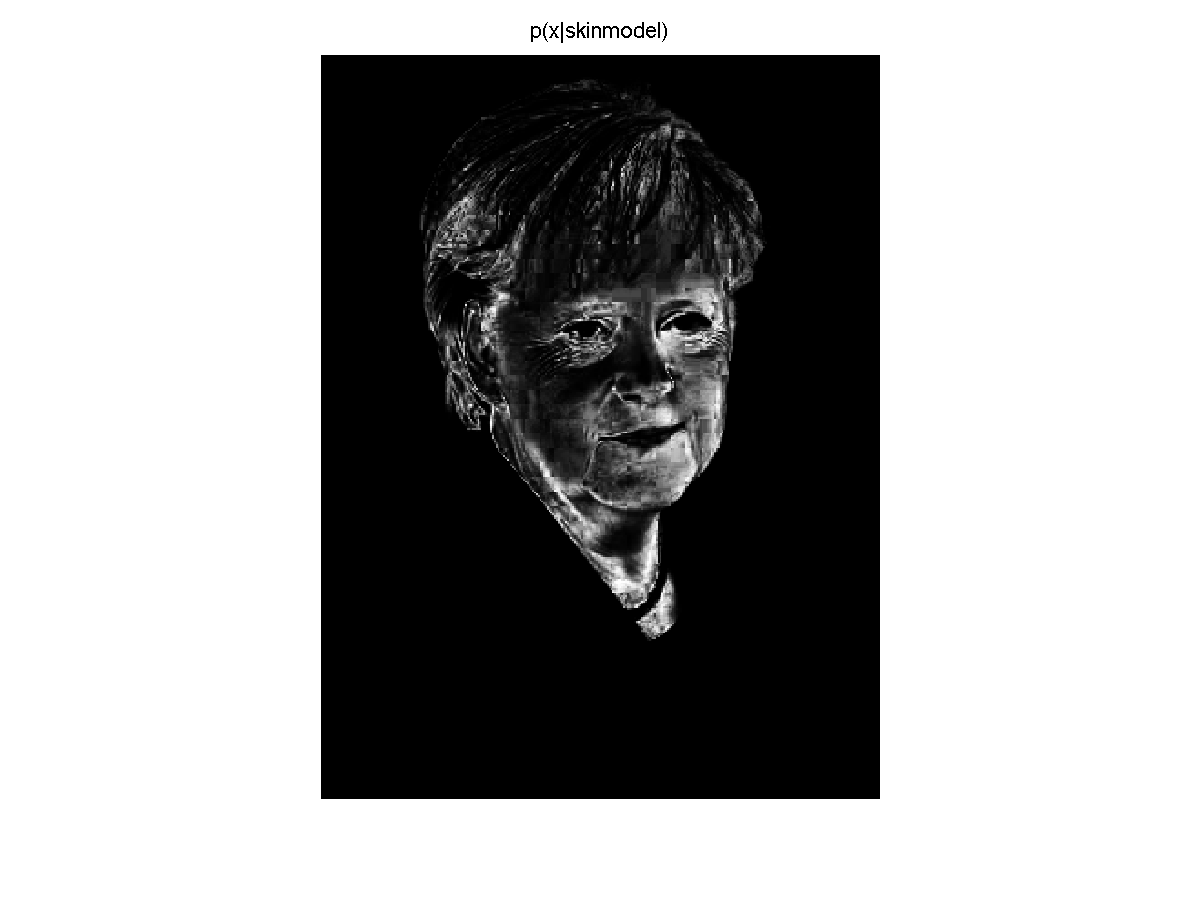
\includegraphics[width=0.5\textwidth]{img/SampleImage-skin.png}
    \caption{Normalized Skin Model Likelihood of SampleImage.png}
    \label{fig:skin1}
\end{figure}
\begin{figure}[h!]
  	\centering
    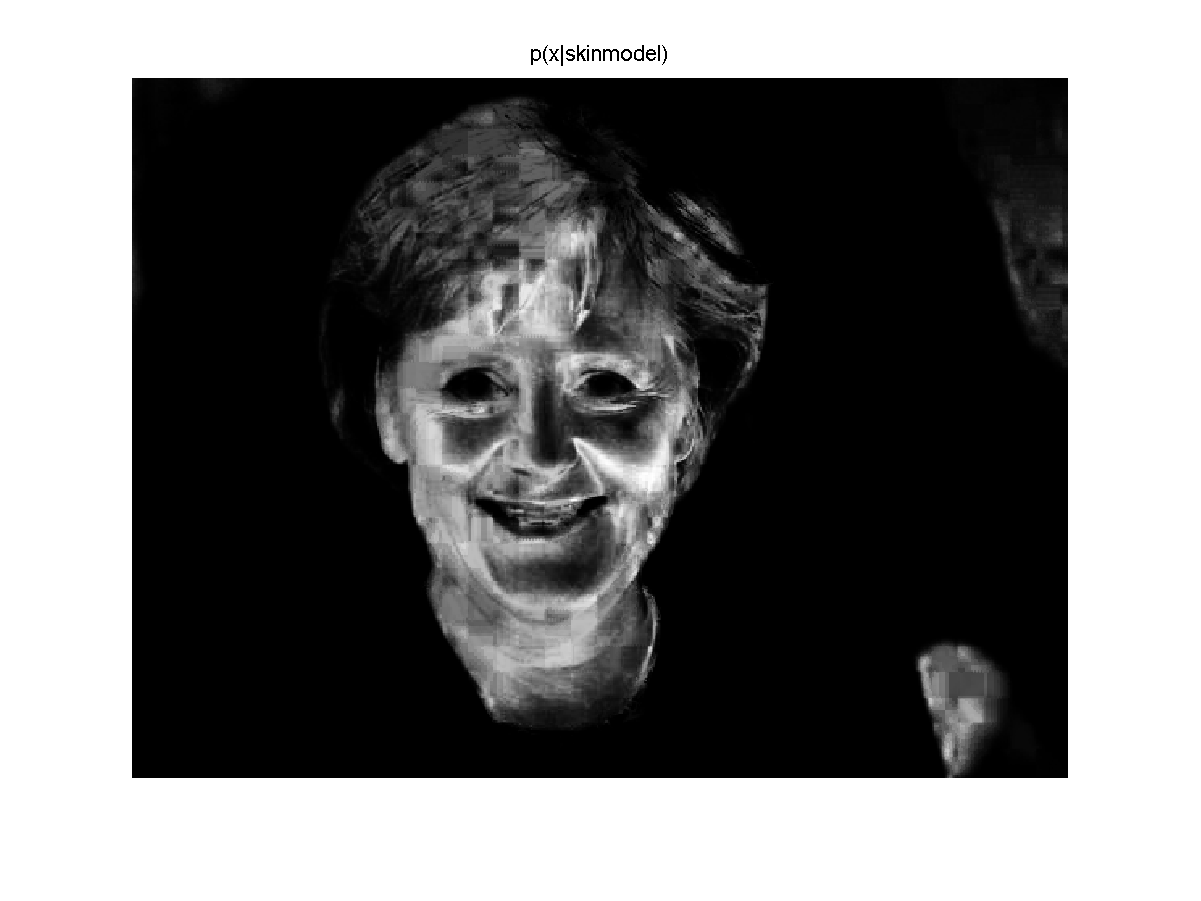
\includegraphics[width=0.5\textwidth]{img/SampleImage2-skin.png}
    \caption{Normalized Skin Model Likelihood of SampleImage2.png}
    \label{fig:skin2}
\end{figure}

\newpage
\item The next pictures (cf. Fig. \ref{fig:back1} and Fig. \ref{fig:back2}) show the normalized LikValues ( $p(x \vert backgroundmodel)$ ) for two unknown pictures
\begin{figure}[h!]
  	\centering
    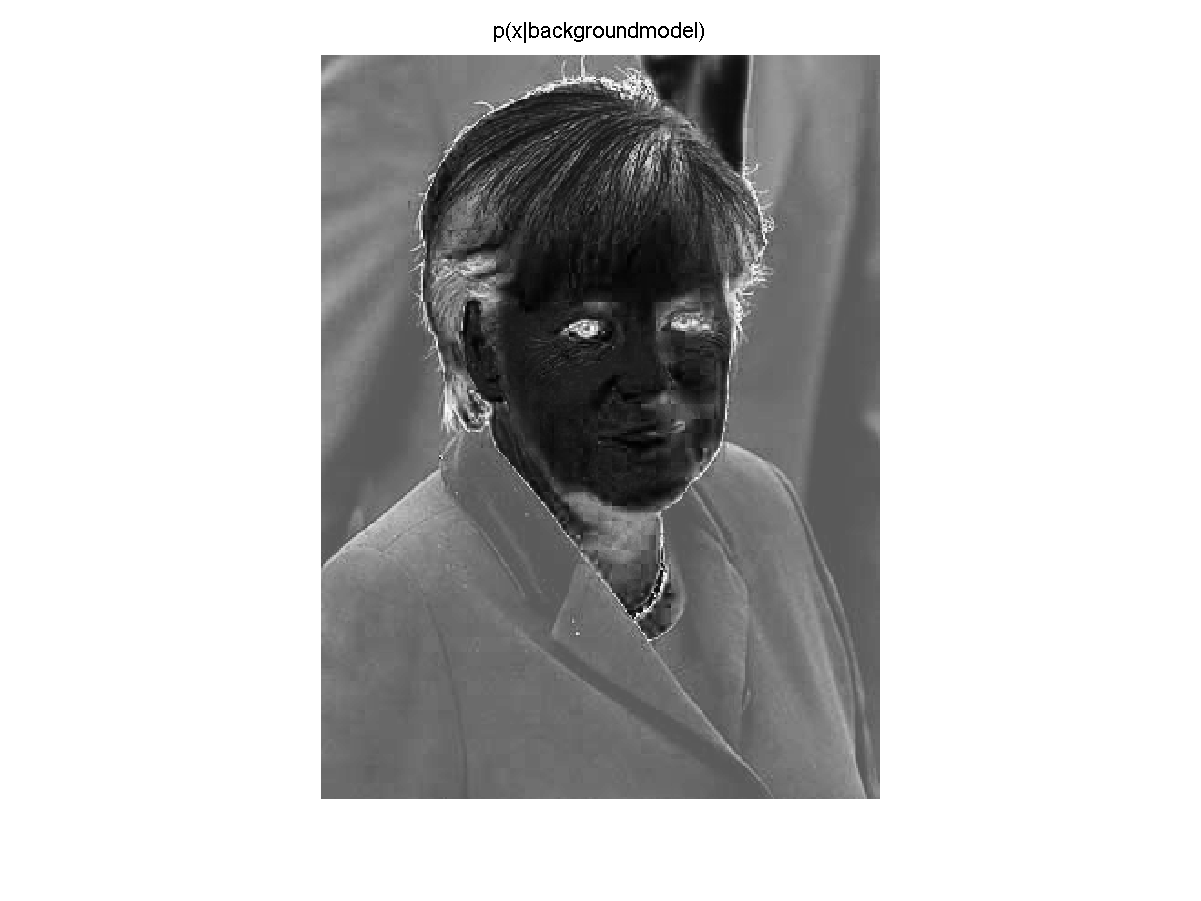
\includegraphics[width=0.5\textwidth]{img/SampleImage-back.png}
    \caption{Normalized Background Model Likelihood of SampleImage.png}
    \label{fig:back1}
\end{figure}
\begin{figure}[h!]
  	\centering
    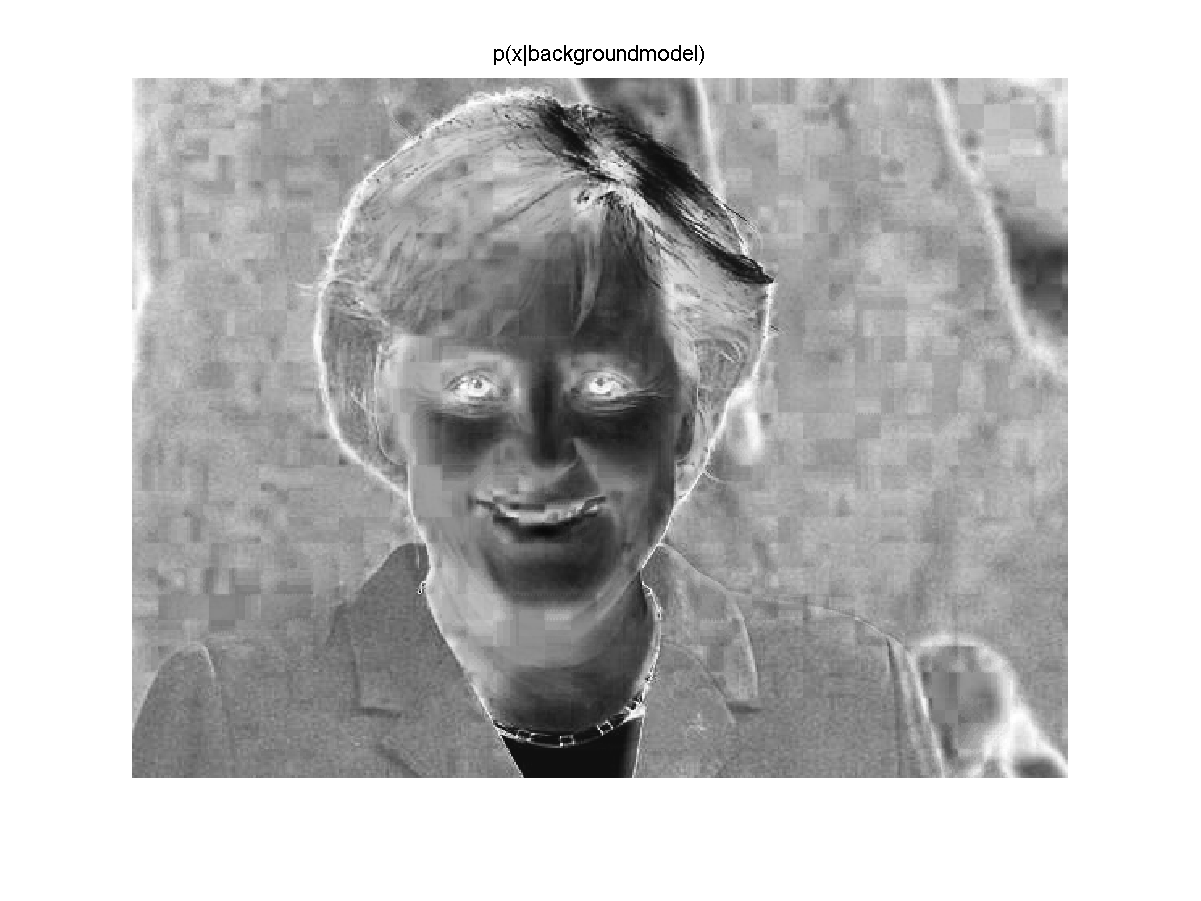
\includegraphics[width=0.5\textwidth]{img/SampleImage2-back.png}
    \caption{Normalized Background Model Likelihood of SampleImage2.png}
    \label{fig:back2}
\end{figure}

\newpage
\item Binary classification images (white belongs most likely to skin, black belongs to background)
\begin{figure}[h!]
  	\centering
    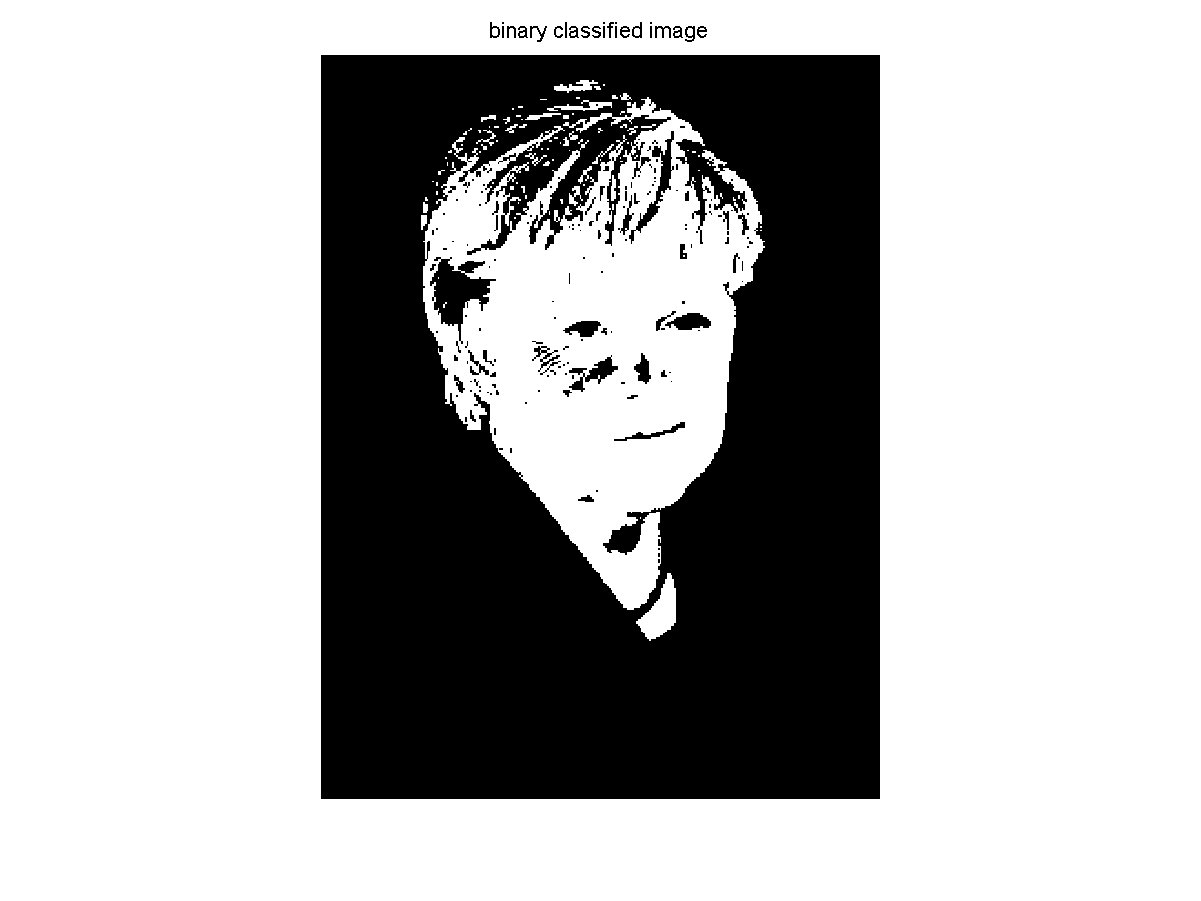
\includegraphics[width=0.5\textwidth]{img/SampleImage-bin.png}
    \caption{Binary classification of SampleImage.png}
    \label{fig:bin1}
\end{figure}
\begin{figure}[h!]
  	\centering
    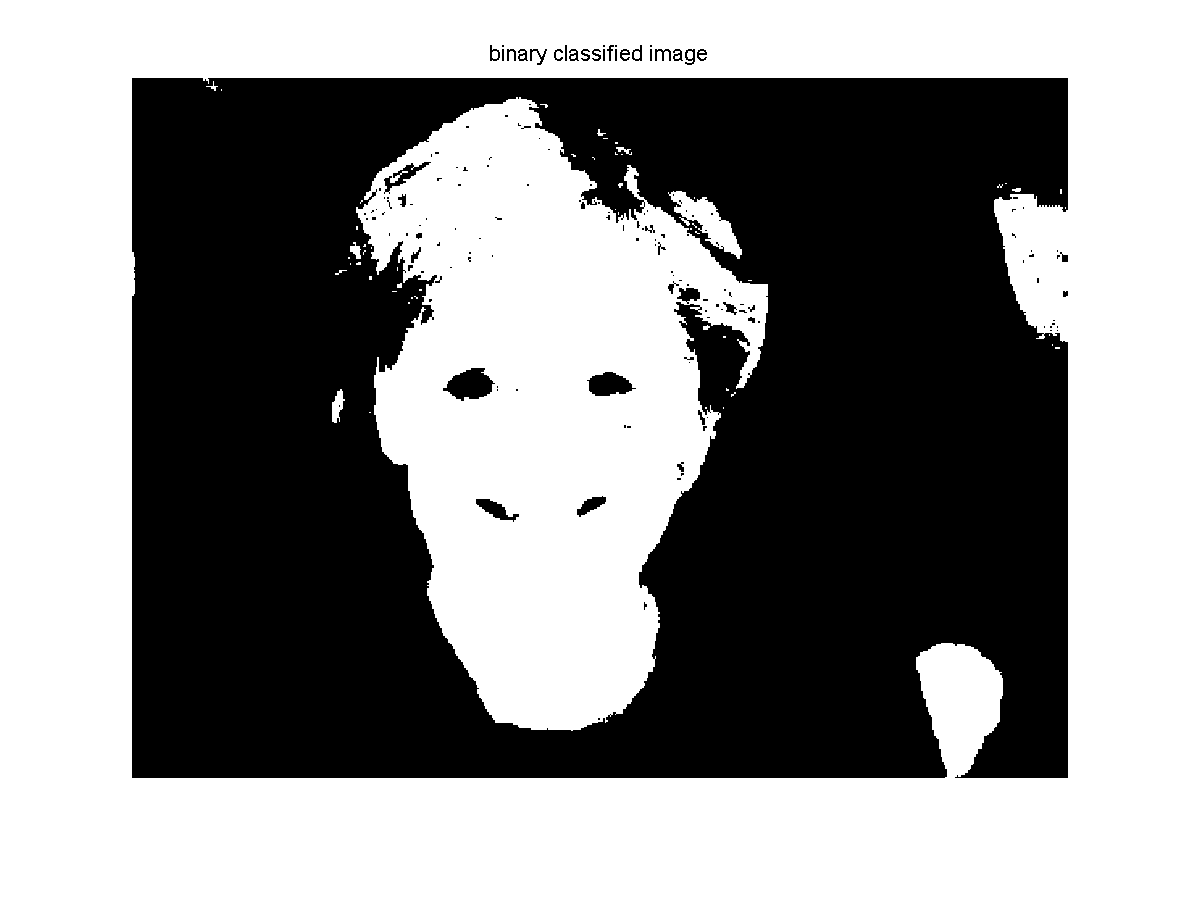
\includegraphics[width=0.5\textwidth]{img/SampleImage2-bin.png}
    \caption{Binary classification of SampleImage2.png}
    \label{fig:bin2}
\end{figure}

\newpage
\item The face area is surrounded by a red rectangle .
\begin{figure}[h!]
  	\centering
    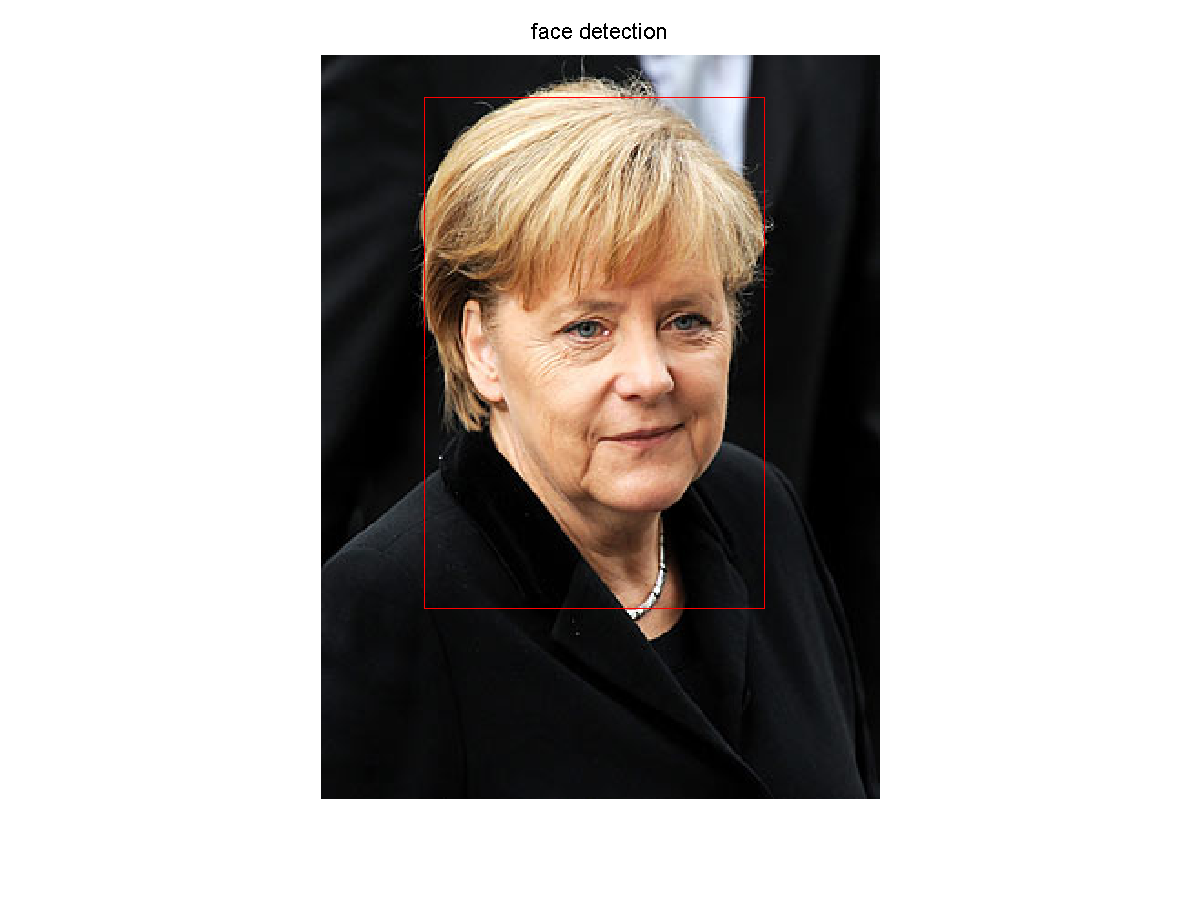
\includegraphics[width=0.5\textwidth]{img/SampleImage-face.png}
    \caption{Face detection of SampleImage.png}
    \label{fig:face1}
\end{figure}
\begin{figure}[h!]
  	\centering
    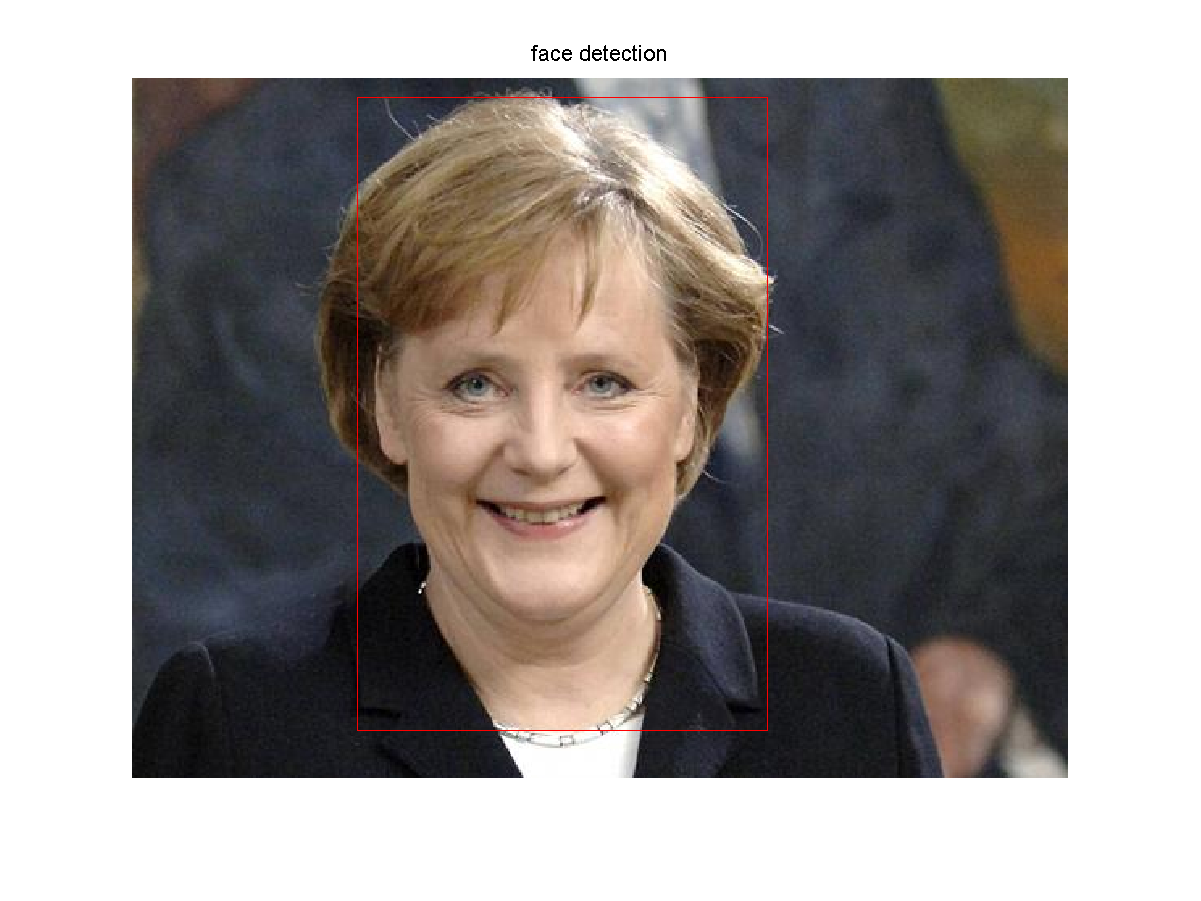
\includegraphics[width=0.5\textwidth]{img/SampleImage2-face.png}
    \caption{Face detection of SampleImage2.png}
    \label{fig:face2}
\end{figure}

\end{compactenum}

\newpage
\section{Exercise}
At first sight one cloud think that the K-means and NUBS algorithm would produce some similar results. But this is only partly true for the o gesture (cf. Fig. \ref{fig:kmean_o} and Fig. \ref{fig:nubs_o}). Even here there a differences in how the points are divided. K-means produces for every gesture a good separation in clear sections of the gesture. NUBS has sometimes problems the divide the sections properly. A good example is the o gesture (cf. Fig. \ref{fig:nubs_o}) where you can find a yellow cluster, a blue cluster an then again a yellow cluster. Especially in the l and x gesture (cf. Fig. \ref{fig:nubs_l}, \ref{fig:nubs_x}) NUBS leads in the x,y space to clusters which are laying above each other. Where as K-means is able to separate also this gestures properly (cf. Fig. \ref{fig:kmean_l}, \ref{fig:kmean_x}). If there would not be the initialization with the same vectors K-means and NUBS would produce a different output every time. But as the clustering results show K-means might be a better tool for gesture recognition. If you don't know which gesture you will have to recognize you would have to choose a random initialization which could lead to bad results. Therefore you could determine some input vectors for the K-means algorithm by first performing the NUBS as a kind of prepossessing. A comparison of the results for the two algorithms can be found below:


\begin{figure}[h!]
  	\centering
    \scalebox{.47}{% This file was created by matlab2tikz.
% Minimal pgfplots version: 1.3
%
%The latest updates can be retrieved from
%  http://www.mathworks.com/matlabcentral/fileexchange/22022-matlab2tikz
%where you can also make suggestions and rate matlab2tikz.
%
\definecolor{mycolor1}{rgb}{1.00000,0.00000,1.00000}%
\definecolor{mycolor2}{rgb}{1.00000,1.00000,0.00000}%
\definecolor{mycolor3}{rgb}{0.00000,1.00000,1.00000}%
%
\begin{tikzpicture}

\begin{axis}[%
width=4.520833in,
height=3.565625in,
at={(0.758333in,0.48125in)},
scale only axis,
separate axis lines,
every outer x axis line/.append style={black},
every x tick label/.append style={font=\color{black}},
xmin=-500,
xmax=500,
xmajorgrids,
every outer y axis line/.append style={black},
every y tick label/.append style={font=\color{black}},
ymin=-400,
ymax=200,
ymajorgrids
]
\addplot [color=blue,only marks,mark=*,mark options={solid},forget plot]
  table[row sep=crcr]{%
275.404877	-242.224854\\
166.773026	-288.660187\\
188.079575	-291.993103\\
207.828308	-295.352753\\
223.496338	-295.475006\\
236.25206	-296.766174\\
247.422836	-295.618256\\
257.021606	-294.221741\\
264.261353	-292.280182\\
265.530853	-289.664154\\
266.843201	-288.621429\\
269.582886	-289.462128\\
171.137482	-322.69873\\
198.408768	-321.025146\\
221.897858	-317.90509\\
240.258438	-313.503265\\
253.406357	-306.325623\\
262.844086	-302.891571\\
269.15799	-297.805939\\
280.27887	-291.162445\\
292.9758	-285.248718\\
303.862061	-279.606506\\
158.227692	-323.858521\\
179.537781	-325.293701\\
204.130585	-325.992188\\
225.425461	-324.62619\\
241.272446	-322.363251\\
255.722809	-316.254181\\
266.656891	-314.33136\\
160.555634	-303.389496\\
185.782349	-306.301971\\
209.38298	-308.094116\\
227.566284	-310.030243\\
244.734482	-309.034973\\
256.405396	-310.154877\\
262.312622	-313.32724\\
275.479675	-314.55722\\
294.514557	-313.463684\\
314.825348	-315.551941\\
330.23233	-313.897461\\
339.220276	-310.819092\\
341.961029	-308.940887\\
165.260468	-329.008423\\
195.600357	-327.891083\\
222.700684	-324.432892\\
245.799194	-321.165466\\
262.893982	-316.283966\\
275.3284	-310.161896\\
285.441132	-306.805969\\
296.363129	-298.064972\\
309.279236	-289.927795\\
143.393433	-325.312744\\
175.579956	-330.300751\\
203.425903	-332.113373\\
225.710342	-335.666473\\
244.081741	-337.443481\\
255.579651	-335.778381\\
263.373871	-336.269775\\
268.233887	-333.856598\\
280.175415	-334.022034\\
291.807983	-329.016052\\
172.596054	-375.614716\\
202.484802	-365.818939\\
235.29538	-355.977325\\
254.284973	-346.327728\\
269.887726	-336.901215\\
284.103638	-326.933105\\
297.158722	-317.466522\\
310.96698	-309.356873\\
158.571564	-343.718872\\
194.49971	-350.345184\\
227.835236	-354.645325\\
251.258011	-351.925446\\
270.605286	-346.58905\\
292.806	-339.282776\\
310.090607	-329.461365\\
327.836517	-322.543671\\
351.682556	-309.230621\\
372.625336	-297.086456\\
390.950958	-288.039673\\
401.291382	-276.846924\\
405.394775	-269.683044\\
406.616058	-262.654968\\
405.516174	-258.91037\\
405.163269	-257.157776\\
135.310623	-302.115112\\
172.117249	-305.689758\\
205.737701	-307.589569\\
234.832504	-305.761292\\
256.713562	-300.322815\\
278.304474	-295.029388\\
294.532196	-287.800873\\
311.603119	-277.244049\\
329.473907	-267.89679\\
347.053772	-260.379242\\
363.635315	-253.694733\\
393.381531	-248.113754\\
406.822113	-244.375031\\
411.466187	-243.536575\\
};
\addplot [color=black,only marks,mark=*,mark options={solid},forget plot]
  table[row sep=crcr]{%
74.532532	-164.33963\\
104.857727	-138.293152\\
129.403763	-110.437561\\
150.500641	-69.381256\\
157.970474	-30.7549\\
160.293304	3.187594\\
145.866364	-265.200562\\
179.941422	-262.331116\\
214.220352	-259.55069\\
234.49704	-255.176025\\
254.301498	-250.26828\\
269.470917	-246.321686\\
102.626862	-186.805908\\
124.266365	-162.484726\\
138.572647	-130.194183\\
147.558533	-99.564751\\
160.356964	-63.345104\\
162.061935	-25.704762\\
107.944733	-168.772736\\
131.602737	-138.685455\\
147.144897	-104.292282\\
158.684647	-63.571732\\
169.836548	-24.11635\\
148.303116	-225.782898\\
172.764053	-199.451584\\
181.056641	-167.345932\\
196.489349	-139.401535\\
213.324783	-100.343437\\
220.567245	-54.10458\\
138.015778	-215.540268\\
160.367661	-184.311798\\
175.242538	-152.907944\\
179.786957	-117.766129\\
197.747803	-71.505028\\
200.576691	-29.329203\\
134.905441	-225.370987\\
163.171631	-198.039581\\
183.310486	-174.807938\\
195.494095	-149.134445\\
203.333801	-117.6782\\
209.172882	-82.986374\\
214.382416	-43.60659\\
156.783752	-229.460327\\
163.351074	-199.015259\\
189.980164	-162.144272\\
200.967148	-122.314072\\
204.028748	-80.883492\\
210.093124	-37.278133\\
120.257851	-222.564697\\
147.394592	-178.220749\\
178.072556	-134.982025\\
180.754379	-92.338913\\
184.973801	-42.295387\\
141.843033	-211.240723\\
168.279602	-182.669876\\
192.38829	-140.502045\\
201.290939	-101.978523\\
206.345032	-62.248451\\
213.609085	-18.931028\\
168.409897	-232.748688\\
185.911499	-202.882828\\
200.489929	-164.24942\\
220.326447	-124.754021\\
240.582718	-76.903564\\
251.959564	-29.283352\\
};
\addplot [color=red,only marks,mark=*,mark options={solid},forget plot]
  table[row sep=crcr]{%
-152.684708	106.99662\\
-171.9021	77.310448\\
-186.418854	43.127567\\
-192.842163	2.910319\\
-192.693817	-37.345055\\
-186.629929	-81.185997\\
-170.213638	-117.888191\\
-150.21582	-151.237946\\
-160.577591	62.314091\\
-169.761978	29.754766\\
-174.342194	-5.243989\\
-174.159454	-40.638371\\
-147.711334	-86.135437\\
-126.921417	-142.452164\\
-169.553223	71.094017\\
-180.937775	29.428661\\
-186.689713	-14.239443\\
-189.854996	-61.108196\\
-164.918518	-126.162178\\
-147.929718	-171.821701\\
-131.50322	70.523628\\
-143.581558	32.791073\\
-143.21019	-8.619284\\
-139.200073	-50.258785\\
-123.472542	-89.230003\\
-99.164238	-148.698181\\
-122.673447	49.737019\\
-132.318863	10.245519\\
-135.204437	-31.85471\\
-120.124268	-73.973717\\
-92.214752	-123.017731\\
-128.23851	41.643951\\
-137.872833	-3.605462\\
-130.577682	-51.076733\\
-111.08326	-118.563362\\
-102.858475	-164.108963\\
-110.241966	66.581253\\
-128.531754	32.246593\\
-142.809311	-6.871559\\
-144.799408	-41.994461\\
-130.347382	-77.464256\\
-114.200829	-125.119965\\
-103.431549	-163.578033\\
-175.959061	66.555031\\
-205.946594	20.896383\\
-234.696884	-27.349567\\
-244.255814	-81.5439\\
-118.461166	29.728224\\
-128.143738	-21.125484\\
-119.825325	-70.031631\\
-85.072586	-157.285568\\
-65.828766	17.183586\\
-66.658104	-27.527773\\
-62.783352	-70.695007\\
-46.7127	-125.512527\\
};
\addplot [color=green,only marks,mark=*,mark options={solid},forget plot]
  table[row sep=crcr]{%
-226.431656	-196.405609\\
-226.634003	-196.994125\\
-227.744995	-195.946503\\
-227.421722	-196.844818\\
-230.330948	-194.736572\\
-228.779129	-195.692276\\
-230.022583	-194.335785\\
-228.223282	-196.699463\\
-228.972	-195.043045\\
-224.996933	-195.550217\\
-220.904282	-195.175629\\
-200.679398	-195.351105\\
-181.610077	-194.38591\\
-335.455688	-227.792114\\
-336.790253	-226.003418\\
-340.250977	-228.073654\\
-336.410583	-231.102463\\
-327.496002	-232.357666\\
-322.201843	-233.551514\\
-312.88266	-236.105637\\
-289.727417	-242.291885\\
-266.303009	-249.177979\\
-232.431152	-256.670929\\
-187.645706	-260.51709\\
-353.091492	-252.729187\\
-353.351959	-253.976364\\
-352.871857	-254.044037\\
-351.269104	-256.096741\\
-347.876892	-259.091248\\
-342.27179	-260.026764\\
-340.996185	-260.581848\\
-338.188995	-262.985748\\
-330.276489	-264.687805\\
-307.718292	-271.856537\\
-277.790985	-277.735626\\
-241.618881	-277.665192\\
-191.762741	-274.743256\\
-365.905609	-247.169449\\
-366.285248	-244.83461\\
-366.926544	-246.458939\\
-365.892548	-245.957413\\
-361.951874	-246.695953\\
-360.366699	-247.812683\\
-357.777405	-248.611237\\
-353.517487	-250.891708\\
-346.003662	-255.357025\\
-332.260498	-258.383575\\
-304.242126	-269.744904\\
-265.837555	-275.014313\\
-220.794418	-280.000854\\
-160.166061	-281.955811\\
-351.786011	-255.503693\\
-349.724915	-256.940796\\
-350.973877	-257.774902\\
-348.954895	-259.608551\\
-342.440186	-261.395172\\
-330.407501	-266.312561\\
-305.496246	-274.344269\\
-276.75412	-278.689911\\
-248.178848	-285.008514\\
-203.352493	-290.130829\\
-353.834564	-254.811218\\
-353.95578	-255.890564\\
-344.537842	-259.288086\\
-341.55835	-258.966461\\
-336.727173	-261.205658\\
-329.884583	-265.318848\\
-321.473175	-268.868195\\
-304.604797	-273.484161\\
-291.239166	-276.793823\\
-267.341461	-280.764435\\
-236.297577	-280.926758\\
-195.619812	-288.206146\\
-410.336182	-281.433014\\
-407.180023	-282.649353\\
-403.03772	-285.849884\\
-386.216553	-295.115662\\
-365.81311	-303.944916\\
-341.525024	-311.131134\\
-309.214417	-318.852112\\
-274.899139	-329.463776\\
-235.464249	-341.665253\\
-177.980881	-352.635864\\
-409.456635	-284.237488\\
-408.64328	-285.191315\\
-407.919464	-286.575867\\
-407.84906	-287.78006\\
-406.887299	-289.941528\\
-404.68454	-293.437042\\
-402.363464	-299.756683\\
-392.052765	-309.941589\\
-376.686493	-316.929047\\
-350.621613	-330.251465\\
-304.656311	-344.546356\\
-256.718475	-356.269012\\
-196.262741	-363.129974\\
-247.072647	-135.769302\\
-246.680481	-186.583588\\
-238.601089	-231.905487\\
-224.999588	-271.097961\\
-196.628387	-294.225708\\
-169.665878	-319.857635\\
-353.874329	-268.059143\\
-358.700714	-269.25592\\
-356.975037	-268.407288\\
-352.977081	-272.623016\\
-350.164886	-277.17099\\
-331.847687	-281.613861\\
-310.601929	-290.603607\\
-284.293335	-296.208618\\
-244.372604	-303.248138\\
-189.624969	-312.856934\\
-330.03006	-285.601715\\
-329.930511	-285.995575\\
-323.946472	-288.913452\\
-316.101105	-291.60614\\
-307.172791	-293.858337\\
-297.58963	-294.552185\\
-285.170959	-295.902344\\
-263.833221	-299.949951\\
-230.077469	-307.585938\\
-191.045288	-313.085388\\
};
\addplot [color=mycolor1,only marks,mark=*,mark options={solid},forget plot]
  table[row sep=crcr]{%
-150.639267	-203.094437\\
-105.129517	-209.321945\\
-56.389248	-210.465866\\
2.646461	-190.364014\\
36.65501	-184.164398\\
-126.564598	-179.583664\\
-99.097046	-204.697647\\
-73.474808	-214.345703\\
-50.219357	-222.341904\\
-6.421686	-239.421997\\
39.381111	-250.479675\\
65.818123	-256.668945\\
107.668922	-263.312073\\
-136.040588	-257.684998\\
-80.544388	-252.873535\\
-9.340266	-231.299835\\
32.748878	-222.310806\\
68.456123	-208.112793\\
-106.410706	-180.69368\\
-85.180435	-211.988953\\
-62.884792	-238.264404\\
-20.247635	-234.363556\\
31.60428	-246.233246\\
59.45245	-263.585358\\
91.711914	-274.727509\\
132.003616	-281.792145\\
-149.424149	-265.435303\\
-100.454147	-253.506668\\
-31.023933	-236.973389\\
30.518612	-215.802383\\
71.623436	-192.777588\\
-127.66922	-210.490143\\
-108.308998	-244.92337\\
-88.84404	-276.735474\\
-30.022263	-267.171936\\
7.402602	-290.89328\\
43.749241	-308.383514\\
86.297287	-319.564758\\
131.599182	-322.039001\\
-105.901787	-284.730133\\
-36.898354	-289.580292\\
22.587368	-277.657135\\
72.225555	-265.658356\\
108.600174	-249.833176\\
-83.497185	-195.420364\\
-72.2696	-222.721588\\
-50.550705	-237.682236\\
-15.006631	-260.019958\\
24.294413	-280.676636\\
46.679386	-300.419617\\
87.165138	-314.913391\\
122.679085	-319.792542\\
-151.155182	-292.443329\\
-105.673752	-290.555054\\
-30.664843	-290.247162\\
21.971346	-278.24115\\
58.480671	-262.196564\\
102.838959	-241.229477\\
-63.811729	-166.617294\\
-52.443924	-212.829483\\
-28.369097	-229.703232\\
27.354347	-251.931534\\
59.846146	-271.038544\\
94.827713	-286.449097\\
128.174377	-296.924316\\
-146.220078	-291.707306\\
-82.896927	-297.398163\\
-21.296696	-293.779114\\
21.425228	-281.305115\\
65.320602	-266.615967\\
103.171799	-249.603531\\
-91.815392	-207.921616\\
-81.658119	-250.933121\\
-40.014126	-252.426498\\
12.88913	-273.751404\\
39.727997	-297.104614\\
69.745865	-313.423187\\
123.722374	-323.680725\\
-120.611992	-357.307068\\
-68.165581	-351.21524\\
-3.532502	-336.357361\\
43.386837	-319.715729\\
88.18119	-296.173126\\
125.971077	-267.293457\\
-90.379204	-199.291656\\
-75.77433	-234.961441\\
-68.846741	-258.3638\\
-25.360821	-256.383972\\
17.681221	-273.147552\\
41.21307	-291.278015\\
76.55584	-304.316376\\
110.075478	-316.228027\\
-131.000626	-361.188416\\
-71.287125	-350.486572\\
-14.504161	-323.482422\\
39.139305	-296.498901\\
78.775909	-262.248993\\
-130.31662	-342.473907\\
-88.349968	-361.776611\\
-51.1441	-378.573151\\
-12.633525	-389.889526\\
33.145905	-391.388245\\
77.121689	-388.600006\\
127.452194	-385.419434\\
-137.114853	-311.970428\\
-81.483376	-305.894257\\
2.324796	-292.165009\\
52.822716	-270.979858\\
98.098099	-243.254364\\
-70.746468	-209.130035\\
-50.145786	-246.327286\\
-10.330317	-260.048828\\
33.760353	-289.726532\\
73.039345	-315.340942\\
114.008957	-332.665253\\
-143.112289	-320.13031\\
-89.238655	-324.592499\\
-26.9772	-321.857697\\
30.363625	-307.473663\\
75.887581	-286.972168\\
121.320602	-262.47345\\
-26.512442	-176.218536\\
-16.294296	-213.372116\\
-0.499356	-249.894196\\
11.250672	-282.80661\\
69.227844	-276.373596\\
100.072205	-290.588501\\
};
\addplot [color=mycolor2,only marks,mark=*,mark options={solid},forget plot]
  table[row sep=crcr]{%
155.249191	31.665106\\
142.90683	71.924751\\
125.985603	97.051582\\
104.802757	119.5112\\
81.309784	139.819031\\
158.062256	11.863544\\
146.607452	37.870701\\
130.881149	73.885963\\
110.263535	102.812454\\
87.110596	123.709137\\
173.002747	13.836603\\
161.107452	51.235722\\
142.815323	87.653587\\
120.10994	111.73098\\
92.191307	136.914474\\
215.462067	-12.760183\\
203.804596	25.126217\\
190.561691	55.613693\\
165.986984	93.798996\\
143.986633	122.984108\\
112.908989	142.161743\\
87.095222	157.372742\\
198.126816	11.662364\\
185.591354	41.495354\\
168.429123	81.25209\\
146.237549	109.50779\\
123.990692	134.008316\\
98.665359	153.016418\\
213.451767	-5.067266\\
205.575439	31.610891\\
192.876663	63.169819\\
172.261398	102.029366\\
152.848907	132.050522\\
127.359543	154.550049\\
101.126846	170.670746\\
211.208054	5.645715\\
200.427917	39.8936\\
187.153198	78.775307\\
169.278076	111.147194\\
147.506363	138.108307\\
119.820671	151.304489\\
92.638077	161.93898\\
180.719971	-0.327357\\
173.746216	36.67828\\
161.018723	81.804726\\
138.550766	115.952957\\
113.891914	140.53096\\
84.927078	157.170792\\
215.90239	24.270336\\
207.0495	60.094563\\
188.913239	92.380699\\
168.055603	120.047737\\
142.867142	143.115204\\
112.491455	161.618423\\
82.717171	167.873169\\
254.703171	14.089244\\
241.535904	51.917847\\
229.989883	89.84304\\
206.838135	119.720383\\
183.859222	145.616333\\
162.069717	165.634796\\
132.617081	177.60788\\
106.603378	182.470764\\
};
\addplot [color=mycolor3,only marks,mark=*,mark options={solid},forget plot]
  table[row sep=crcr]{%
54.514072	156.379807\\
23.922958	169.633911\\
-4.015235	174.11821\\
-28.959944	174.506699\\
-54.22953	170.317764\\
-82.731628	163.493637\\
-107.346497	148.543457\\
-132.051682	130.746094\\
58.233452	139.776825\\
25.903324	151.157639\\
-9.94149	158.625473\\
-41.26804	158.967194\\
-70.711288	156.707993\\
-97.094254	141.244003\\
-124.525505	123.41227\\
-148.819168	100.232536\\
63.111629	156.331238\\
30.002644	171.504623\\
-5.420382	179.362915\\
-36.719246	176.114258\\
-70.845757	169.346786\\
-98.55426	156.786469\\
-124.679375	139.69313\\
-151.322388	113.699188\\
54.409138	170.203796\\
20.206131	177.724991\\
-14.23244	176.376099\\
-41.854916	170.173431\\
-68.968002	156.531403\\
-92.070442	135.520065\\
-115.391464	109.566582\\
71.04969	169.835876\\
32.401577	169.148102\\
-4.368976	169.333252\\
-37.292316	163.346817\\
-65.80323	150.005508\\
-93.742065	129.128265\\
-112.056023	89.453407\\
71.215126	182.592575\\
30.777126	180.646133\\
-4.400435	175.235016\\
-35.323425	167.259415\\
-65.891075	152.413269\\
-88.904396	125.365417\\
-112.30732	84.684822\\
60.821388	167.256287\\
25.724182	165.933167\\
-8.154403	151.054337\\
-39.177197	138.658768\\
-63.165268	119.863449\\
-87.259483	95.895897\\
53.064472	171.861252\\
4.316373	170.141251\\
-35.66349	164.64093\\
-76.314117	154.633926\\
-113.759766	140.153336\\
-146.87764	110.406319\\
44.11557	164.117767\\
7.394058	161.612381\\
-23.578817	153.66716\\
-53.766335	130.152145\\
-78.277504	100.097984\\
-101.145462	67.938431\\
76.733971	183.344788\\
45.120117	175.826141\\
10.927358	152.894608\\
-17.707668	127.14003\\
-34.720928	100.523537\\
-52.755596	59.412937\\
};
\end{axis}
\end{tikzpicture}%}
    \caption{K-means on gesture l}
    \label{fig:kmean_l}
\end{figure}
\vspace{-10pt}
\begin{figure}[h!]
  	\centering
    \scalebox{.47}{% This file was created by matlab2tikz.
% Minimal pgfplots version: 1.3
%
%The latest updates can be retrieved from
%  http://www.mathworks.com/matlabcentral/fileexchange/22022-matlab2tikz
%where you can also make suggestions and rate matlab2tikz.
%
\definecolor{mycolor1}{rgb}{1.00000,0.00000,1.00000}%
\definecolor{mycolor2}{rgb}{1.00000,1.00000,0.00000}%
\definecolor{mycolor3}{rgb}{0.00000,1.00000,1.00000}%
%
\begin{tikzpicture}

\begin{axis}[%
width=4.520833in,
height=3.565625in,
at={(0.758333in,0.48125in)},
scale only axis,
separate axis lines,
every outer x axis line/.append style={black},
every x tick label/.append style={font=\color{black}},
xmin=-400,
xmax=400,
xmajorgrids,
every outer y axis line/.append style={black},
every y tick label/.append style={font=\color{black}},
ymin=-500,
ymax=200,
ymajorgrids
]
\addplot [color=blue,only marks,mark=*,mark options={solid},forget plot]
  table[row sep=crcr]{%
171.69873	154.395508\\
203.537384	144.42598\\
238.47908	118.089714\\
270.850616	90.097679\\
303.503052	53.652573\\
333.515808	10.419273\\
350.695251	-46.217243\\
355.75116	-96.06118\\
151.514618	121.60202\\
187.794754	107.930305\\
226.158096	85.771706\\
261.141296	57.593567\\
284.933563	20.929031\\
307.929016	-18.688892\\
316.526001	-55.798122\\
312.799103	-97.42688\\
140.146652	115.995552\\
180.321793	94.252838\\
223.926315	65.871887\\
254.398956	24.031935\\
277.604828	-23.875883\\
298.136993	-79.21035\\
159.133392	108.80394\\
195.072006	89.311218\\
231.210312	60.262135\\
258.656128	27.550968\\
277.414795	-26.116282\\
293.677612	-86.695892\\
163.556351	110.073967\\
198.630814	91.952095\\
230.667068	68.754158\\
257.76593	38.987602\\
279.792267	5.140823\\
298.465027	-34.762535\\
308.631866	-77.926956\\
170.128876	132.802567\\
201.436218	115.318794\\
235.150116	90.473595\\
266.369385	47.285114\\
293.593445	-2.99046\\
306.2771	-65.91893\\
137.5271	111.033379\\
169.86586	95.312027\\
209.525681	64.256607\\
235.026596	24.909536\\
255.126114	-18.445982\\
271.450348	-70.317131\\
132.948151	99.303047\\
169.967697	76.506409\\
205.883804	37.709953\\
236.001541	-1.181519\\
254.956116	-55.781265\\
151.505157	65.913506\\
177.078857	29.157312\\
192.596756	-16.992109\\
195.243149	-75.715332\\
191.039581	-114.400192\\
153.175003	111.27639\\
180.837051	85.217545\\
205.934448	62.968876\\
229.065979	33.793732\\
249.091812	-0.36778\\
253.785538	-50.030937\\
259.653351	-95.703629\\
};
\addplot [color=black,only marks,mark=*,mark options={solid},forget plot]
  table[row sep=crcr]{%
-139.771927	-414.697815\\
-190.291031	-408.904907\\
-236.300491	-397.548553\\
-268.950195	-367.290405\\
-283.87088	-331.833038\\
-296.476715	-293.855103\\
-301.986603	-256.376831\\
-142.125137	-411.074066\\
-186.340805	-406.990875\\
-229.70253	-398.668213\\
-272.45517	-383.576569\\
-291.052704	-350.672516\\
-305.258667	-314.195007\\
-312.562134	-277.730865\\
-181.330994	-424.074432\\
-198.868805	-405.034973\\
-214.808167	-378.881134\\
-224.840179	-352.944244\\
-232.912476	-321.764709\\
-295.321899	-266.0867\\
-183.259018	-439.432098\\
-225.620728	-432.328705\\
-288.008698	-415.892975\\
-309.181702	-383.858521\\
-317.638062	-344.930634\\
-319.665863	-303.343109\\
-318.299011	-263.202759\\
-170.133575	-434.228119\\
-215.583038	-433.68277\\
-282.730927	-428.749664\\
-345.603455	-413.287628\\
-371.736328	-373.691711\\
-388.954437	-330.93042\\
-391.241547	-283.179871\\
-174.775223	-422.936798\\
-221.586914	-411.202881\\
-258.96405	-377.655823\\
-277.282166	-335.24173\\
-286.80188	-292.366608\\
-295.428528	-248.091812\\
-147.84436	-416.244781\\
-202.214142	-413.960175\\
-258.547058	-404.971191\\
-292.612976	-373.196167\\
-307.700439	-330.361359\\
-317.740814	-287.234589\\
-321.327759	-240.174301\\
-189.078568	-427.94754\\
-240.769623	-417.263214\\
-282.700195	-387.861206\\
-297.801941	-340.745392\\
-295.852722	-290.947388\\
-291.775543	-242.927155\\
-150.588104	-386.60144\\
-181.773239	-372.885101\\
-209.737534	-356.927887\\
-240.769104	-334.64444\\
-271.113037	-305.599243\\
-285.186157	-276.791229\\
-300.295807	-243.545303\\
-145.671432	-362.00885\\
-179.008987	-341.574554\\
-196.390411	-314.749146\\
-216.273224	-283.262726\\
-231.961655	-249.554657\\
};
\addplot [color=red,only marks,mark=*,mark options={solid},forget plot]
  table[row sep=crcr]{%
355.8172	-143.556854\\
332.643829	-191.59317\\
327.935791	-237.357956\\
319.674225	-282.434387\\
305.993866	-328.869812\\
285.632782	-371.605011\\
242.968414	-399.36673\\
182.851868	-410.651428\\
301.65564	-136.00209\\
299.788391	-178.331482\\
297.244965	-221.495285\\
285.648651	-264.405151\\
272.744904	-302.227692\\
256.673065	-347.052216\\
226.751678	-386.503265\\
190.364914	-408.450806\\
304.886078	-137.301758\\
300.352142	-189.77803\\
292.44455	-241.042984\\
256.982513	-291.320618\\
218.470657	-324.473816\\
181.165268	-367.306366\\
277.916656	-154.108292\\
252.514206	-209.932236\\
246.253754	-264.750336\\
240.395294	-309.905334\\
218.756622	-364.948212\\
191.167877	-405.927826\\
316.572601	-117.10553\\
315.821655	-157.843475\\
292.539673	-202.144775\\
278.551727	-248.612839\\
258.32962	-290.607605\\
235.928421	-339.9245\\
199.573456	-378.5448\\
153.640366	-402.881073\\
289.505157	-127.528465\\
282.366364	-178.203644\\
270.509644	-230.843765\\
257.480469	-278.004364\\
241.337738	-318.199646\\
212.388901	-364.275635\\
175.109863	-398.045898\\
261.897339	-124.094116\\
244.301819	-177.072418\\
233.517838	-236.136414\\
217.936493	-280.106842\\
195.950073	-330.843506\\
157.661118	-372.900055\\
247.950073	-120.156319\\
242.228104	-173.823578\\
230.750336	-231.415268\\
218.78981	-277.417694\\
200.816345	-328.336212\\
169.612167	-377.585327\\
172.410736	-181.724564\\
150.275848	-229.747406\\
124.527458	-265.58432\\
92.134155	-300.874634\\
258.922699	-132.294571\\
250.1418	-172.332855\\
232.825623	-211.881989\\
199.76561	-253.833176\\
162.071075	-287.900757\\
112.940186	-320.916901\\
};
\addplot [color=green,only marks,mark=*,mark options={solid},forget plot]
  table[row sep=crcr]{%
-295.873413	-217.575516\\
-305.692261	-177.904068\\
-301.628571	-148.284561\\
-291.525848	-120.806267\\
-283.020233	-90.372375\\
-272.811981	-62.338261\\
-266.264984	-39.48122\\
-256.730621	-12.952227\\
-312.84848	-240.435257\\
-316.42807	-202.643799\\
-313.625092	-168.166397\\
-312.997131	-130.563309\\
-303.622772	-97.208984\\
-290.995819	-66.285599\\
-280.150391	-36.210995\\
-272.229462	-3.849154\\
-263.254913	23.118263\\
-306.847504	-221.786087\\
-304.240143	-187.021118\\
-300.037018	-156.10791\\
-295.416016	-116.53199\\
-288.849548	-82.712021\\
-283.52066	-53.132736\\
-273.276489	-21.343582\\
-256.25766	-1.252498\\
-319.534576	-223.518097\\
-320.620544	-181.402557\\
-307.186737	-148.113571\\
-294.212341	-113.369545\\
-288.806946	-74.350372\\
-284.757568	-38.444145\\
-277.635925	-6.161349\\
-262.854889	9.842613\\
-372.351746	-239.427353\\
-364.97287	-186.666\\
-344.789612	-146.237274\\
-325.817627	-110.850189\\
-314.724152	-84.44944\\
-303.480072	-39.39624\\
-290.232574	0.537766\\
-292.038391	-207.902161\\
-292.882477	-177.430252\\
-285.602325	-143.590881\\
-290.706451	-89.801231\\
-282.605896	-46.118938\\
-262.499664	-15.354491\\
-317.491364	-197.543015\\
-309.035278	-155.146622\\
-294.887146	-114.634407\\
-283.946564	-72.100838\\
-278.758698	-29.089554\\
-267.110748	13.704705\\
-287.034851	-199.018768\\
-285.300568	-165.082794\\
-275.849091	-125.538651\\
-273.591644	-69.468674\\
-256.257385	-36.402473\\
-234.005814	-10.736093\\
-311.597717	-204.997681\\
-321.716797	-168.060333\\
-320.724152	-130.211533\\
-316.614319	-92.404709\\
-307.447296	-56.100117\\
-299.515778	-23.231741\\
-290.639709	6.204737\\
-244.793655	-213.210892\\
-254.73111	-177.207565\\
-260.34964	-133.262604\\
-261.031738	-89.842651\\
-255.726608	-50.371536\\
-245.473846	-16.623457\\
};
\addplot [color=mycolor1,only marks,mark=*,mark options={solid},forget plot]
  table[row sep=crcr]{%
16.643066	161.905502\\
27.753811	162.423538\\
41.409824	161.386459\\
57.533684	161.741592\\
77.853188	163.662292\\
97.576317	165.826462\\
121.563408	164.107346\\
145.719772	158.591629\\
-70.67968	134.159821\\
-57.685379	134.826828\\
-47.807186	132.058868\\
-41.987476	128.923096\\
-34.964783	130.165726\\
-28.866335	135.576385\\
-27.56881	135.819794\\
-22.521999	136.830231\\
-14.484533	138.845749\\
-1.00687	136.928421\\
15.852446	140.587646\\
50.446365	136.665375\\
82.981339	136.372696\\
116.717339	131.895248\\
-54.033569	147.702316\\
-47.91272	150.717361\\
-35.038033	152.33783\\
-8.983257	152.421921\\
21.783209	151.892685\\
62.781597	140.320435\\
103.474968	132.040771\\
-68.888931	121.581245\\
-60.136925	123.36232\\
-53.718204	127.549728\\
-49.111511	127.649811\\
-44.012928	127.65303\\
-42.144226	126.499161\\
-43.161842	142.194687\\
-42.147293	143.13501\\
-38.5257	142.934662\\
-29.841879	144.296432\\
-17.433643	145.559738\\
-1.40561	146.010406\\
20.874601	146.978851\\
57.033783	140.137741\\
90.993141	135.231842\\
127.687256	125.787369\\
-68.054489	110.247322\\
-60.284397	110.313927\\
-53.946404	110.142036\\
-23.994217	134.067474\\
-18.05814	135.296127\\
-7.407155	136.186005\\
7.730005	138.398666\\
36.079124	134.497971\\
64.268661	131.880234\\
96.62561	128.771133\\
131.99939	123.190048\\
-71.951675	135.521164\\
-58.626358	135.150787\\
-48.485085	134.282471\\
-42.089417	133.785965\\
-38.299549	131.107742\\
-33.909332	131.542404\\
-24.785444	158.396027\\
-19.188185	159.60376\\
-10.791924	159.48114\\
-0.53068	159.346725\\
16.978142	156.952789\\
37.316021	156.716202\\
58.228127	159.139297\\
86.304016	158.810974\\
113.511391	153.907288\\
142.663788	144.150116\\
-70.370743	143.486465\\
-51.511616	144.764114\\
-34.659935	144.219894\\
-17.024876	143.315353\\
-3.321425	139.183426\\
4.137576	137.72525\\
8.742867	135.848785\\
11.124843	132.4216\\
13.041642	129.40683\\
14.567312	128.493851\\
37.96384	130.92009\\
55.280327	132.182709\\
79.133873	130.52121\\
107.694786	120.474236\\
-87.843605	137.245941\\
-67.197487	143.726089\\
-48.62112	144.427261\\
-30.019667	143.383377\\
-16.225512	138.806076\\
-6.179718	134.491257\\
3.098855	132.787933\\
10.431727	128.894943\\
16.587427	127.052872\\
20.550104	123.952774\\
25.294731	121.731644\\
26.790249	120.075714\\
28.577106	117.894287\\
29.058954	115.909615\\
29.282595	114.510628\\
29.533693	114.034683\\
27.276419	113.100121\\
10.92443	119.693336\\
25.189489	117.055237\\
46.441624	115.599953\\
71.680511	115.257881\\
101.914635	110.031769\\
-69.203636	133.889236\\
-49.632248	135.532272\\
-27.669609	134.599121\\
-7.451278	131.851562\\
7.210238	127.686256\\
21.045311	123.123871\\
32.64658	118.89476\\
39.892654	116.751472\\
45.256763	113.572418\\
47.935242	108.380333\\
46.683506	107.256599\\
45.945938	106.03228\\
44.7178	105.200172\\
43.735966	103.623077\\
42.299114	101.108932\\
39.518291	101.722511\\
35.636765	101.052155\\
-84.439468	115.624382\\
-81.363525	116.669327\\
-78.604378	117.539917\\
-74.732285	118.352386\\
-61.289089	119.979881\\
-44.088188	123.402367\\
-17.822819	125.920288\\
15.193284	123.755829\\
54.718254	118.483917\\
91.195	108.279465\\
121.20256	95.655113\\
-87.916969	135.950272\\
-67.582512	139.674973\\
-49.042572	139.929184\\
-34.626568	134.52916\\
-22.275135	128.486221\\
-14.504045	123.193283\\
-7.401706	119.185265\\
-2.884366	115.29364\\
-1.234767	113.409477\\
-2.139737	112.4356\\
-3.180743	110.837257\\
-4.897582	108.027496\\
-44.220734	124.767982\\
-40.360477	128.480576\\
-33.889267	129.176636\\
-25.355488	129.882339\\
-11.800712	134.17099\\
7.878999	137.697952\\
34.242535	139.351334\\
65.266426	135.303909\\
92.508308	131.558105\\
124.88517	121.51181\\
-77.293121	151.873032\\
-55.659225	155.911255\\
-36.899513	156.177597\\
-14.599265	154.160767\\
6.972499	152.57312\\
27.334578	147.519714\\
41.73999	145.312881\\
51.717487	144.684982\\
49.815365	138.596451\\
48.980598	133.263397\\
49.030304	133.87439\\
49.99445	131.612305\\
47.601944	131.403671\\
};
\addplot [color=mycolor2,only marks,mark=*,mark options={solid},forget plot]
  table[row sep=crcr]{%
122.31147	-415.089783\\
73.667427	-417.314362\\
27.811069	-416.994873\\
-12.423848	-415.583618\\
-46.488708	-412.33551\\
-88.942139	-416.778076\\
142.575882	-414.489227\\
96.348679	-418.764984\\
47.564075	-416.981964\\
7.435687	-415.097931\\
-27.321274	-411.240601\\
-61.119427	-413.276154\\
-99.161087	-412.958801\\
138.861267	-398.227295\\
92.809761	-424.211395\\
44.220802	-443.765839\\
2.921609	-455.980377\\
-35.090527	-446.105042\\
-64.719986	-443.203552\\
-91.945183	-444.195007\\
-122.001762	-442.000153\\
-153.158875	-434.378754\\
141.520264	-430.941315\\
100.138374	-441.491425\\
56.305882	-447.200928\\
19.112078	-451.845215\\
-15.759893	-454.602875\\
-49.590862	-456.307404\\
-73.954376	-454.279144\\
-98.16996	-452.256134\\
-123.608795	-449.97229\\
-150.634552	-446.094971\\
98.554413	-414.623962\\
48.26178	-419.254242\\
7.960542	-427.89267\\
-33.80764	-433.241272\\
-66.359756	-434.009064\\
-97.691956	-435.174866\\
-132.772217	-434.756256\\
124.813217	-413.891388\\
79.852463	-419.035645\\
38.623627	-422.198181\\
-1.22965	-424.858612\\
-38.772137	-425.097504\\
-77.103271	-426.61554\\
-123.239449	-429.265717\\
108.515907	-397.81723\\
63.618153	-406.247559\\
20.277376	-412.240448\\
-23.032387	-415.488312\\
-59.537281	-415.50235\\
-96.830536	-413.180939\\
126.208733	-408.810303\\
80.736618	-420.155518\\
38.695118	-425.338623\\
0.654602	-435.511993\\
-38.70425	-439.503479\\
-68.897087	-437.694733\\
-100.436462	-435.332153\\
-140.469437	-433.219574\\
53.694881	-334.256226\\
7.333529	-357.321869\\
-36.680676	-375.0737\\
-70.770233	-384.941742\\
-106.139969	-389.912476\\
69.888939	-345.259766\\
26.764214	-361.329376\\
-19.702642	-367.0867\\
-60.744354	-375.761108\\
-103.307625	-370.521576\\
};
\addplot [color=mycolor3,only marks,mark=*,mark options={solid},forget plot]
  table[row sep=crcr]{%
-235.11525	23.341619\\
-216.633865	41.909279\\
-197.81987	58.98357\\
-181.61972	73.079132\\
-164.899551	87.412788\\
-146.81456	103.902077\\
-131.722839	112.271919\\
-115.48468	120.378334\\
-101.75502	127.322922\\
-85.963799	130.596542\\
-250.326019	44.430527\\
-228.29158	28.725534\\
-213.55365	44.350163\\
-198.112396	60.978626\\
-184.401413	74.399849\\
-168.701797	86.527924\\
-157.28186	96.487801\\
-142.00972	103.528404\\
-129.386475	109.070061\\
-116.119217	112.012955\\
-101.831184	114.033516\\
-93.740547	115.935043\\
-243.344711	21.167433\\
-225.157532	40.046402\\
-208.280228	58.417774\\
-189.401245	73.026642\\
-174.30748	85.886597\\
-158.627396	97.133034\\
-141.737488	105.970886\\
-127.835762	110.717545\\
-113.341072	114.153435\\
-99.65078	117.923668\\
-89.356583	118.829041\\
-79.548569	119.653847\\
-245.331238	25.100752\\
-223.157867	41.574188\\
-196.118103	57.158447\\
-175.260452	72.11232\\
-156.36499	83.113403\\
-137.610809	92.819023\\
-121.247559	100.31218\\
-104.797478	103.542076\\
-89.946503	105.138084\\
-78.932251	108.297462\\
-270.105743	26.043188\\
-245.82489	50.110596\\
-220.584808	66.491119\\
-196.760559	83.43557\\
-176.037384	98.193504\\
-155.645905	113.065163\\
-138.480362	120.016563\\
-122.296883	127.659637\\
-102.622849	133.45401\\
-86.410553	135.038483\\
-240.503906	14.573446\\
-217.043762	40.505188\\
-193.814285	63.636429\\
-173.158951	88.926346\\
-150.212296	109.040077\\
-129.78949	120.953705\\
-111.434753	133.030426\\
-90.679153	139.773987\\
-255.330429	21.767336\\
-226.334381	41.271774\\
-201.537582	59.659424\\
-182.672699	83.443268\\
-163.786133	99.288727\\
-146.792297	109.880081\\
-127.971695	122.050461\\
-107.85788	130.146667\\
-213.690536	21.996853\\
-194.991302	48.753883\\
-176.184784	72.649956\\
-155.543365	93.136513\\
-135.64296	105.914581\\
-112.870369	118.768288\\
-90.276131	128.027115\\
-275.689941	32.47097\\
-258.88678	54.19418\\
-234.39534	71.281487\\
-212.181549	89.199745\\
-190.112991	106.198509\\
-168.704224	116.949913\\
-149.00322	125.025024\\
-127.029716	132.132507\\
-107.444756	132.215057\\
-228.049103	14.542366\\
-210.439743	42.651863\\
-193.210892	72.242584\\
-176.554932	100.331528\\
-156.597351	120.519569\\
-138.137634	133.577591\\
-120.761841	145.769333\\
-99.332527	149.518204\\
};
\end{axis}
\end{tikzpicture}%}
    \caption{K-means on gesture o}
    \label{fig:kmean_o}
\end{figure}
\vspace{-10pt}
\begin{figure}[h!]
  	\centering
    \scalebox{.47}{% This file was created by matlab2tikz.
% Minimal pgfplots version: 1.3
%
%The latest updates can be retrieved from
%  http://www.mathworks.com/matlabcentral/fileexchange/22022-matlab2tikz
%where you can also make suggestions and rate matlab2tikz.
%
\definecolor{mycolor1}{rgb}{1.00000,0.00000,1.00000}%
\definecolor{mycolor2}{rgb}{1.00000,1.00000,0.00000}%
\definecolor{mycolor3}{rgb}{0.00000,1.00000,1.00000}%
%
\begin{tikzpicture}

\begin{axis}[%
width=4.520833in,
height=3.565625in,
at={(0.758333in,0.48125in)},
scale only axis,
separate axis lines,
every outer x axis line/.append style={black},
every x tick label/.append style={font=\color{black}},
xmin=-500,
xmax=300,
xmajorgrids,
every outer y axis line/.append style={black},
every y tick label/.append style={font=\color{black}},
ymin=-500,
ymax=300,
ymajorgrids
]
\addplot [color=blue,only marks,mark=*,mark options={solid},forget plot]
  table[row sep=crcr]{%
-300.344727	190.460037\\
-293.159088	194.46405\\
-280.589996	191.786804\\
-378.478455	200.453125\\
-377.031158	220.352417\\
-371.703674	233.732849\\
-364.827026	240.258759\\
-358.517273	242.860565\\
-344.438416	237.596573\\
-329.240234	227.333923\\
-312.058563	214.556335\\
-291.640961	197.08252\\
-391.83017	190.860733\\
-379.786713	211.235504\\
-368.652161	227.450836\\
-357.419647	236.415268\\
-346.18869	242.332886\\
-337.561401	241.847015\\
-330.236847	244.040787\\
-318.780365	240.471771\\
-301.512085	229.0383\\
-281.997986	215.805847\\
-263.590576	198.38208\\
-243.047653	179.002655\\
-336.90506	158.80275\\
-328.475281	182.097565\\
-324.232178	202.143707\\
-316.639893	216.463989\\
-306.13623	217.052887\\
-298.328491	218.426071\\
-288.950317	214.549393\\
-276.665405	207.546234\\
-263.549744	191.770386\\
-245.106445	168.124588\\
-211.556412	150.843002\\
-300.654694	146.669464\\
-298.773682	181.113159\\
-292.821747	207.053055\\
-285.051941	226.817017\\
-278.001495	237.678741\\
-271.962769	244.357498\\
-262.773438	242.844162\\
-252.815231	244.098175\\
-240.066223	242.147263\\
-223.266434	231.757141\\
-200.595703	207.829544\\
-171.875061	180.175323\\
-140.648605	152.233231\\
-103.423096	122.733551\\
-304.997345	142.02449\\
-307.120056	173.045334\\
-306.249756	196.764511\\
-301.584167	214.232559\\
-296.8591	225.296173\\
-288.649872	229.006027\\
-282.217865	230.063766\\
-272.262054	225.247742\\
-258.489197	218.148254\\
-243.764999	205.894928\\
-224.117889	190.279434\\
-208.506851	176.258087\\
-186.363068	163.458023\\
-159.89502	143.353256\\
-122.657036	110.776962\\
-326.195465	132.145096\\
-314.722931	140.310959\\
-303.607361	142.11702\\
-293.886566	140.618851\\
-277.429749	129.493088\\
-257.561523	115.011398\\
-332.174194	121.79174\\
-327.333557	154.133255\\
-319.841278	181.596603\\
-316.272644	196.98912\\
-309.318024	212.607941\\
-304.038879	220.654236\\
-295.74704	225.172211\\
-286.069427	224.847961\\
-278.08432	223.386459\\
-264.45929	217.52478\\
-246.089462	206.717667\\
-227.87384	192.567764\\
-209.312241	170.392899\\
-169.014343	147.032089\\
-122.47625	116.885109\\
-324.082031	129.892578\\
-317.420349	161.68071\\
-313.585693	190.647858\\
-313.877655	210.609711\\
-311.605255	225.95314\\
-344.183472	251.681015\\
-344.183472	251.681015\\
-344.183472	251.681015\\
-344.183472	251.681015\\
-344.183472	251.681015\\
-344.183472	251.681015\\
-344.183472	251.681015\\
-344.183472	251.681015\\
-344.183472	251.681015\\
-344.183472	251.681015\\
-344.183472	251.681015\\
-344.183472	251.681015\\
-344.183472	251.681015\\
-344.183472	251.681015\\
-344.183472	251.681015\\
-344.183472	251.681015\\
-344.183472	251.681015\\
-344.183472	251.681015\\
-344.183472	251.681015\\
-344.183472	251.681015\\
-344.183472	251.681015\\
-344.183472	251.681015\\
-344.183472	251.681015\\
-344.183472	251.681015\\
-344.183472	251.681015\\
-276.647186	140.049301\\
-278.951843	169.616211\\
-280.032867	196.697601\\
-245.508545	196.031097\\
-245.508545	196.031097\\
-253.508636	220.018661\\
-253.508636	220.018661\\
-251.238586	219.304214\\
-251.238586	219.304214\\
-234.426895	208.203308\\
-234.426895	208.203308\\
-200.56369	195.121887\\
-200.56369	195.121887\\
-147.882095	173.106384\\
-147.882095	173.106384\\
-147.882095	173.106384\\
-147.882095	173.106384\\
-147.882095	173.106384\\
-147.882095	173.106384\\
-147.882095	173.106384\\
-147.882095	173.106384\\
-147.882095	173.106384\\
-147.882095	173.106384\\
-147.882095	173.106384\\
-147.882095	173.106384\\
-147.882095	173.106384\\
-147.882095	173.106384\\
-147.882095	173.106384\\
-147.882095	173.106384\\
-147.882095	173.106384\\
-147.882095	173.106384\\
-147.882095	173.106384\\
};
\addplot [color=black,only marks,mark=*,mark options={solid},forget plot]
  table[row sep=crcr]{%
169.81218	-157.056976\\
196.40451	-179.411514\\
209.505112	-197.195862\\
213.565155	-210.37738\\
218.362244	-216.776474\\
219.948792	-220.884125\\
220.205521	-222.29184\\
221.126389	-222.632202\\
220.407578	-223.570099\\
218.845535	-223.840561\\
215.752747	-223.486725\\
214.678375	-223.362869\\
212.827118	-224.023514\\
156.688248	-160.524399\\
179.989838	-190.733566\\
193.696259	-214.19519\\
202.688583	-229.877487\\
205.195053	-239.754669\\
207.613449	-245.611191\\
210.744858	-247.985001\\
211.987228	-248.561447\\
212.356918	-247.202911\\
211.982651	-245.496643\\
146.645309	-177.803818\\
179.33638	-215.065323\\
201.021011	-245.557693\\
212.155304	-267.508362\\
219.559433	-281.632812\\
143.452576	-164.784973\\
178.977142	-200.349625\\
202.115112	-226.488602\\
220.452408	-245.20961\\
230.024231	-257.263428\\
233.50531	-264.911621\\
240.05896	-266.357513\\
241.252579	-266.359924\\
244.203903	-266.838013\\
243.049774	-263.972626\\
246.579987	-261.058807\\
140.57756	-146.223633\\
174.377686	-186.993866\\
196.411819	-216.754715\\
215.15123	-238.675476\\
225.772766	-253.787186\\
227.533859	-262.25705\\
229.162918	-267.035583\\
182.585266	-155.065765\\
214.825302	-192.946335\\
238.278702	-220.796921\\
257.443848	-245.156921\\
267.098816	-260.738495\\
275.502991	-272.168152\\
279.433258	-280.469299\\
107.924934	-216.95491\\
146.689072	-265.703979\\
185.685486	-305.500458\\
209.912781	-332.433014\\
222.7724	-349.79306\\
230.780121	-361.989777\\
235.647339	-371.40448\\
239.862869	-374.88266\\
242.503021	-375.961273\\
250.237244	-376.395355\\
253.397491	-374.215668\\
257.872986	-371.963562\\
190.037827	-173.711502\\
223.811783	-214.650528\\
241.987854	-240.428558\\
253.140045	-258.640778\\
275.389038	-276.873352\\
286.371033	-285.511658\\
};
\addplot [color=red,only marks,mark=*,mark options={solid},forget plot]
  table[row sep=crcr]{%
152.651535	50.053802\\
145.439545	45.396988\\
184.520752	80.321068\\
181.26944	80.148102\\
180.120819	75.492599\\
172.764038	68.208549\\
158.522247	59.837585\\
138.319489	39.728958\\
178.18512	127.415337\\
176.674072	127.40979\\
175.350693	126.233841\\
171.760406	123.047195\\
166.066406	119.490753\\
154.460602	110.561882\\
141.29689	100.588005\\
126.46843	90.730804\\
232.945328	133.206314\\
231.323914	133.040131\\
225.738464	129.508484\\
219.66124	130.053101\\
209.166428	125.828957\\
197.845932	115.039711\\
182.420151	102.174995\\
144.691162	62.267593\\
254.962448	108.367752\\
254.093658	107.629097\\
255.152847	108.504402\\
253.50972	108.366936\\
249.987137	106.708557\\
245.336258	103.272903\\
241.687866	101.53019\\
236.215683	99.743538\\
224.825943	89.817047\\
211.977921	75.517471\\
186.43129	50.828545\\
135.372604	12.39957\\
284.208771	132.398895\\
281.745483	128.930679\\
280.082184	127.389664\\
275.759766	125.194511\\
268.694092	123.216293\\
258.292023	114.424347\\
248.82579	108.544647\\
231.075562	99.865593\\
194.792358	67.807335\\
157.446716	35.510185\\
120.625275	1.085071\\
193.034286	53.442162\\
169.512207	33.665192\\
145.319168	13.420936\\
284.988708	119.735321\\
282.403778	119.204735\\
275.745239	119.472946\\
266.943451	119.418396\\
262.065033	117.188072\\
261.001495	116.344383\\
253.968567	115.785393\\
246.34491	113.760422\\
231.208206	110.72345\\
212.907822	105.357674\\
174.384964	79.308258\\
139.829315	55.970337\\
100.497795	25.252048\\
255.531296	118.000175\\
252.098373	120.628403\\
246.388199	120.17263\\
234.42189	116.653336\\
214.395569	108.978256\\
189.872665	92.773438\\
144.744949	52.266964\\
104.968376	22.008694\\
127.589897	134.66713\\
117.689514	129.673706\\
101.349899	120.908836\\
65.339478	77.948921\\
};
\addplot [color=green,only marks,mark=*,mark options={solid},forget plot]
  table[row sep=crcr]{%
-128.237701	-211.299973\\
-128.237701	-211.299973\\
-171.328888	-268.307953\\
-213.35173	-296.580597\\
-240.739777	-317.38797\\
-257.049408	-328.077148\\
-269.708771	-325.717407\\
-272.631866	-311.224487\\
-272.458252	-284.803192\\
-269.841003	-252.519516\\
-268.303802	-214.794754\\
-270.779144	-172.479889\\
-274.481781	-143.113281\\
-273.603485	-101.212708\\
-125.76239	-194.39949\\
-137.097885	-228.830231\\
-168.264877	-240.298553\\
-203.25119	-272.358765\\
-231.462143	-297.687988\\
-250.18927	-314.855804\\
-265.612183	-318.512726\\
-278.491791	-311.166473\\
-289.346985	-291.296143\\
-299.583038	-267.387665\\
-309.331055	-234.927353\\
-311.311615	-197.303116\\
-319.141541	-158.284576\\
-353.034698	-125.203743\\
-144.042786	-153.138779\\
-151.731857	-197.849121\\
-169.464096	-225.654984\\
-187.634262	-244.858612\\
-204.630493	-257.578949\\
-215.358673	-261.518463\\
-219.721909	-261.247589\\
-217.82933	-253.630783\\
-203.82016	-239.389328\\
-193.548721	-225.764908\\
-190.396774	-209.309189\\
-186.932266	-194.017761\\
-186.094894	-175.845612\\
-193.584839	-156.256226\\
-193.944763	-137.233734\\
-198.643463	-116.021812\\
-199.340973	-93.963043\\
-99.912071	-174.018097\\
-137.396973	-214.322205\\
-167.809402	-245.709656\\
-202.712585	-287.180359\\
-232.862457	-317.721863\\
-255.953125	-336.94693\\
-304.300415	-304.723114\\
-314.019623	-273.401703\\
-321.205963	-237.750671\\
-325.34024	-194.991837\\
-332.168762	-159.553101\\
-328.55069	-116.553574\\
-92.646156	-183.926804\\
-94.079285	-217.750488\\
-129.913818	-249.483032\\
-165.615051	-281.060394\\
-186.821167	-306.673676\\
-210.108124	-319.977295\\
-224.617783	-325.554077\\
-237.186691	-322.648376\\
-246.237396	-313.570709\\
-250.325531	-299.899628\\
-254.650085	-280.219299\\
-254.270676	-249.743591\\
-257.293823	-216.15593\\
-261.076172	-177.003525\\
-278.038391	-149.310684\\
-278.816498	-102.60482\\
-94.27549	-208.068253\\
-123.000824	-232.311249\\
-149.660614	-254.500351\\
-174.437683	-270.895203\\
-188.688965	-278.346497\\
-204.628601	-283.108337\\
-214.703857	-279.207092\\
-223.945892	-267.262207\\
-231.937943	-250.761871\\
-240.895782	-226.100494\\
-246.802811	-194.910507\\
-256.059509	-160.003891\\
-269.347778	-131.256027\\
-62.788116	-224.227448\\
-94.444801	-254.491211\\
-131.714706	-278.866669\\
-174.869827	-322.884216\\
-375.181702	-264.126221\\
-376.679138	-202.951981\\
-363.359467	-134.962463\\
-110.557961	-174.913971\\
-153.997131	-203.311157\\
-181.29187	-235.646057\\
-206.358292	-262.676697\\
-229.064163	-283.884552\\
-250.660706	-296.491516\\
-271.25592	-299.179535\\
-280.683533	-291.548187\\
-288.077057	-274.945068\\
-297.760651	-249.162476\\
-303.167297	-214.581818\\
-310.720673	-172.978668\\
-325.095184	-130.037399\\
-104.521782	-169.5186\\
-131.994476	-196.324036\\
-175.784805	-220.313538\\
-207.150848	-251.554565\\
-236.056381	-274.406647\\
-262.835541	-292.043335\\
-278.597992	-299.694519\\
-288.996094	-300.514893\\
-296.250427	-294.036926\\
-296.592438	-279.073059\\
-301.856445	-258.038574\\
-302.069672	-226.462616\\
-304.889191	-189.028244\\
-306.462006	-149.499725\\
-319.186462	-104.610832\\
-144.329865	-143.642441\\
-174.295364	-175.809708\\
-194.561218	-182.958115\\
-219.976089	-197.126205\\
-238.516754	-210.108337\\
-251.877029	-214.04541\\
-260.921295	-211.826324\\
-266.670044	-203.276306\\
-273.692871	-189.559296\\
-278.589203	-170.390411\\
-277.373779	-146.981277\\
-281.65152	-119.943893\\
-288.641357	-95.805344\\
};
\addplot [color=mycolor1,only marks,mark=*,mark options={solid},forget plot]
  table[row sep=crcr]{%
-274.880859	-343.775665\\
-287.947784	-340.779327\\
-296.43515	-326.055664\\
-216.107025	-363.004913\\
-257.840973	-398.221954\\
-287.919525	-428.888855\\
-319.247894	-454.366791\\
-339.634369	-466.45105\\
-357.821167	-471.9646\\
-372.607269	-472.02832\\
-377.157471	-461.625793\\
-378.807068	-442.690216\\
-376.247101	-411.420685\\
-377.546783	-369.332642\\
-377.386658	-320.256653\\
};
\addplot [color=mycolor2,only marks,mark=*,mark options={solid},forget plot]
  table[row sep=crcr]{%
135.139893	37.056835\\
126.280235	27.554398\\
112.626328	17.92408\\
94.902832	-0.286605\\
70.797813	-21.974504\\
28.417324	-64.533279\\
-14.268426	-99.16835\\
-38.02562	-123.043282\\
-71.564613	-157.20459\\
-98.791809	70.845116\\
-30.092646	8.751842\\
23.864695	-28.329626\\
82.768448	-63.380661\\
100.945648	-92.122566\\
142.933472	-126.734032\\
118.576508	22.377728\\
93.020508	2.937385\\
55.799305	-33.766399\\
-2.47515	-82.942619\\
-34.621254	-111.649788\\
-67.427757	-145.209717\\
-107.74424	57.234257\\
-56.942772	11.663648\\
-1.553901	-47.417587\\
80.523773	-82.223358\\
121.95076	-117.742996\\
94.4813	62.597797\\
54.540592	25.756941\\
4.435115	-16.959824\\
-41.614235	-47.570309\\
-84.442902	-99.245918\\
-102.896469	60.802662\\
-30.21475	-3.639842\\
26.124554	-50.143997\\
26.124554	-50.143997\\
111.338882	-136.58812\\
107.679901	27.131542\\
70.467415	-7.351249\\
8.099855	-62.294029\\
-37.134895	-100.916718\\
-59.880413	11.336433\\
-6.155514	-40.743336\\
-6.155514	-40.743336\\
101.058937	-118.276939\\
97.902054	-23.50876\\
28.703545	-89.457756\\
-19.461086	-126.677895\\
-61.479034	70.418976\\
6.57631	-4.577844\\
73.985519	-53.485783\\
91.556671	-105.337189\\
71.927589	-52.624943\\
18.958246	-100.156746\\
-28.180021	-141.621704\\
-75.23481	-188.864944\\
-57.648476	46.308376\\
-7.558801	-4.074922\\
57.456924	-48.610893\\
94.960358	-84.540421\\
125.301788	-120.228096\\
122.937386	-9.417118\\
93.776939	-42.838993\\
64.224724	-71.892746\\
29.570812	-105.831947\\
7.870351	-138.378754\\
-18.783777	-173.095428\\
-131.579285	-16.844603\\
-71.91143	-45.61351\\
-19.319427	-87.615883\\
35.538174	-136.068176\\
66.43586	-168.885498\\
42.56311	-29.411739\\
0.38504	-69.365776\\
-36.256382	-112.494881\\
-80.149887	-157.500046\\
-37.047749	44.471115\\
5.934473	-22.106167\\
91.883385	-58.998428\\
136.830795	-116.303093\\
49.219986	-34.369244\\
-12.002185	-80.919472\\
-53.813019	-126.412018\\
33.089321	52.745003\\
-1.089752	21.457006\\
-38.672905	-18.367807\\
-75.694191	-67.873657\\
-104.01889	-104.565536\\
};
\addplot [color=mycolor3,only marks,mark=*,mark options={solid},forget plot]
  table[row sep=crcr]{%
-288.136963	-54.082638\\
-305.550323	-8.843312\\
-317.286285	48.137165\\
-319.446625	89.555649\\
-316.317871	124.189819\\
-313.713348	150.745544\\
-312.285248	170.237564\\
-305.573578	184.284561\\
-269.950836	185.949768\\
-246.869843	168.58432\\
-217.842651	149.76149\\
-187.817749	130.547363\\
-151.109848	108.429947\\
-348.427429	-85.655655\\
-350.631073	-40.339653\\
-363.912323	5.274295\\
-378.860992	58.591667\\
-379.191925	103.123566\\
-379.982269	139.474838\\
-379.26825	172.938568\\
-263.308655	176.787704\\
-216.484894	146.390549\\
-169.56871	114.568687\\
-377.809814	19.905254\\
-377.809814	19.905254\\
-406.800995	99.858719\\
-411.706635	136.242447\\
-403.505249	164.363876\\
-217.88475	158.569458\\
-189.743683	137.626785\\
-155.019623	113.7733\\
-334.471008	-70.650772\\
-337.658783	-15.975376\\
-343.180908	38.649925\\
-343.541779	83.488197\\
-339.807068	123.74012\\
-175.51976	126.110031\\
-131.652496	57.49268\\
-276.52356	-52.442192\\
-279.39679	0.569284\\
-286.907104	51.59848\\
-297.162842	100.596535\\
-268.777771	-88.695908\\
-276.693329	-42.959042\\
-286.283264	15.124262\\
-300.094025	65.648933\\
-302.031219	106.280159\\
-357.388947	-71.668114\\
-337.67099	-48.400284\\
-340.601013	0.925131\\
-346.140198	55.551479\\
-343.308716	89.067612\\
-339.163452	115.587624\\
-235.823044	98.902733\\
-203.701874	65.06369\\
-162.946243	28.693356\\
-333.196259	-80.008789\\
-349.518433	-25.993177\\
-327.698944	-2.690661\\
-335.839935	46.221115\\
-334.09494	84.342026\\
-320.724976	-65.795761\\
-320.668274	-14.859903\\
-326.435181	36.439747\\
-332.737244	84.304817\\
-265.134796	-80.290031\\
-272.087524	-47.012142\\
-279.139465	-6.32836\\
-285.999481	34.069931\\
-281.363037	80.129974\\
-278.854279	111.096893\\
};
\end{axis}
\end{tikzpicture}%}
    \caption{K-means on gesture x}
    \label{fig:kmean_x}
\end{figure}
\vspace{-20pt}
\begin{figure}[h!]
  	\centering
    \scalebox{.47}{% This file was created by matlab2tikz.
% Minimal pgfplots version: 1.3
%
%The latest updates can be retrieved from
%  http://www.mathworks.com/matlabcentral/fileexchange/22022-matlab2tikz
%where you can also make suggestions and rate matlab2tikz.
%
\definecolor{mycolor1}{rgb}{1.00000,0.00000,1.00000}%
\definecolor{mycolor2}{rgb}{1.00000,1.00000,0.00000}%
\definecolor{mycolor3}{rgb}{0.00000,1.00000,1.00000}%
%
\begin{tikzpicture}

\begin{axis}[%
width=4.520833in,
height=3.565625in,
at={(0.758333in,0.48125in)},
scale only axis,
separate axis lines,
every outer x axis line/.append style={black},
every x tick label/.append style={font=\color{black}},
xmin=-500,
xmax=500,
xmajorgrids,
every outer y axis line/.append style={black},
every y tick label/.append style={font=\color{black}},
ymin=-400,
ymax=200,
ymajorgrids
]
\addplot [color=blue,only marks,mark=*,mark options={solid},forget plot]
  table[row sep=crcr]{%
-226.431656	-196.405609\\
-226.634003	-196.994125\\
-227.744995	-195.946503\\
-227.421722	-196.844818\\
-230.330948	-194.736572\\
-228.779129	-195.692276\\
-230.022583	-194.335785\\
-228.223282	-196.699463\\
-228.972	-195.043045\\
-224.996933	-195.550217\\
-220.904282	-195.175629\\
-200.679398	-195.351105\\
-181.610077	-194.38591\\
-150.639267	-203.094437\\
-335.455688	-227.792114\\
-336.790253	-226.003418\\
-340.250977	-228.073654\\
-336.410583	-231.102463\\
-327.496002	-232.357666\\
-322.201843	-233.551514\\
-312.88266	-236.105637\\
-289.727417	-242.291885\\
-266.303009	-249.177979\\
-232.431152	-256.670929\\
-187.645706	-260.51709\\
-136.040588	-257.684998\\
-80.544388	-252.873535\\
-353.091492	-252.729187\\
-353.351959	-253.976364\\
-352.871857	-254.044037\\
-351.269104	-256.096741\\
-347.876892	-259.091248\\
-342.27179	-260.026764\\
-340.996185	-260.581848\\
-338.188995	-262.985748\\
-330.276489	-264.687805\\
-307.718292	-271.856537\\
-277.790985	-277.735626\\
-241.618881	-277.665192\\
-191.762741	-274.743256\\
-149.424149	-265.435303\\
-100.454147	-253.506668\\
-127.66922	-210.490143\\
-108.308998	-244.92337\\
-88.84404	-276.735474\\
-365.905609	-247.169449\\
-366.285248	-244.83461\\
-366.926544	-246.458939\\
-365.892548	-245.957413\\
-361.951874	-246.695953\\
-360.366699	-247.812683\\
-357.777405	-248.611237\\
-353.517487	-250.891708\\
-346.003662	-255.357025\\
-332.260498	-258.383575\\
-304.242126	-269.744904\\
-265.837555	-275.014313\\
-220.794418	-280.000854\\
-160.166061	-281.955811\\
-105.901787	-284.730133\\
-351.786011	-255.503693\\
-349.724915	-256.940796\\
-350.973877	-257.774902\\
-348.954895	-259.608551\\
-342.440186	-261.395172\\
-330.407501	-266.312561\\
-305.496246	-274.344269\\
-276.75412	-278.689911\\
-248.178848	-285.008514\\
-203.352493	-290.130829\\
-151.155182	-292.443329\\
-105.673752	-290.555054\\
-353.834564	-254.811218\\
-353.95578	-255.890564\\
-344.537842	-259.288086\\
-341.55835	-258.966461\\
-336.727173	-261.205658\\
-329.884583	-265.318848\\
-321.473175	-268.868195\\
-304.604797	-273.484161\\
-291.239166	-276.793823\\
-267.341461	-280.764435\\
-236.297577	-280.926758\\
-195.619812	-288.206146\\
-146.220078	-291.707306\\
-82.896927	-297.398163\\
-410.336182	-281.433014\\
-407.180023	-282.649353\\
-403.03772	-285.849884\\
-386.216553	-295.115662\\
-365.81311	-303.944916\\
-341.525024	-311.131134\\
-309.214417	-318.852112\\
-274.899139	-329.463776\\
-235.464249	-341.665253\\
-177.980881	-352.635864\\
-120.611992	-357.307068\\
-68.165581	-351.21524\\
-409.456635	-284.237488\\
-408.64328	-285.191315\\
-407.919464	-286.575867\\
-407.84906	-287.78006\\
-406.887299	-289.941528\\
-404.68454	-293.437042\\
-402.363464	-299.756683\\
-392.052765	-309.941589\\
-376.686493	-316.929047\\
-350.621613	-330.251465\\
-304.656311	-344.546356\\
-256.718475	-356.269012\\
-196.262741	-363.129974\\
-131.000626	-361.188416\\
-71.287125	-350.486572\\
-244.255814	-81.5439\\
-247.072647	-135.769302\\
-246.680481	-186.583588\\
-238.601089	-231.905487\\
-224.999588	-271.097961\\
-196.628387	-294.225708\\
-169.665878	-319.857635\\
-130.31662	-342.473907\\
-88.349968	-361.776611\\
-51.1441	-378.573151\\
-12.633525	-389.889526\\
33.145905	-391.388245\\
-353.874329	-268.059143\\
-358.700714	-269.25592\\
-356.975037	-268.407288\\
-352.977081	-272.623016\\
-350.164886	-277.17099\\
-331.847687	-281.613861\\
-310.601929	-290.603607\\
-284.293335	-296.208618\\
-244.372604	-303.248138\\
-189.624969	-312.856934\\
-137.114853	-311.970428\\
-81.483376	-305.894257\\
-330.03006	-285.601715\\
-329.930511	-285.995575\\
-323.946472	-288.913452\\
-316.101105	-291.60614\\
-307.172791	-293.858337\\
-297.58963	-294.552185\\
-285.170959	-295.902344\\
-263.833221	-299.949951\\
-230.077469	-307.585938\\
-191.045288	-313.085388\\
-143.112289	-320.13031\\
-89.238655	-324.592499\\
-26.9772	-321.857697\\
};
\addplot [color=black,only marks,mark=*,mark options={solid},forget plot]
  table[row sep=crcr]{%
138.572647	-130.194183\\
147.558533	-99.564751\\
-124.525505	123.41227\\
-148.819168	100.232536\\
-160.577591	62.314091\\
-169.761978	29.754766\\
-126.921417	-142.452164\\
-106.410706	-180.69368\\
188.079575	-291.993103\\
207.828308	-295.352753\\
-151.322388	113.699188\\
-169.553223	71.094017\\
-180.937775	29.428661\\
198.408768	-321.025146\\
221.897858	-317.90509\\
172.764053	-199.451584\\
181.056641	-167.345932\\
-115.391464	109.566582\\
-131.50322	70.523628\\
-143.581558	32.791073\\
-143.21019	-8.619284\\
-139.200073	-50.258785\\
-99.164238	-148.698181\\
-83.497185	-195.420364\\
-72.2696	-222.721588\\
122.679085	-319.792542\\
158.227692	-323.858521\\
179.537781	-325.293701\\
160.367661	-184.311798\\
-112.056023	89.453407\\
-122.673447	49.737019\\
-132.318863	10.245519\\
-135.204437	-31.85471\\
-120.124268	-73.973717\\
-92.214752	-123.017731\\
-63.811729	-166.617294\\
-52.443924	-212.829483\\
128.174377	-296.924316\\
160.555634	-303.389496\\
185.782349	-306.301971\\
183.310486	-174.807938\\
195.494095	-149.134445\\
-112.30732	84.684822\\
-128.23851	41.643951\\
-111.08326	-118.563362\\
-102.858475	-164.108963\\
195.600357	-327.891083\\
222.700684	-324.432892\\
163.351074	-199.015259\\
189.980164	-162.144272\\
-110.241966	66.581253\\
-128.531754	32.246593\\
-142.809311	-6.871559\\
-114.200829	-125.119965\\
-103.431549	-163.578033\\
-90.379204	-199.291656\\
-75.77433	-234.961441\\
143.393433	-325.312744\\
175.579956	-330.300751\\
203.425903	-332.113373\\
235.29538	-355.977325\\
254.284973	-346.327728\\
-101.145462	67.938431\\
-118.461166	29.728224\\
-128.143738	-21.125484\\
-119.825325	-70.031631\\
-85.072586	-157.285568\\
-70.746468	-209.130035\\
-50.145786	-246.327286\\
158.571564	-343.718872\\
194.49971	-350.345184\\
227.835236	-354.645325\\
185.911499	-202.882828\\
-52.755596	59.412937\\
-65.828766	17.183586\\
-66.658104	-27.527773\\
-62.783352	-70.695007\\
-46.7127	-125.512527\\
-26.512442	-176.218536\\
-16.294296	-213.372116\\
-0.499356	-249.894196\\
11.250672	-282.80661\\
100.072205	-290.588501\\
135.310623	-302.115112\\
172.117249	-305.689758\\
};
\addplot [color=red,only marks,mark=*,mark options={solid},forget plot]
  table[row sep=crcr]{%
160.356964	-63.345104\\
162.061935	-25.704762\\
158.062256	11.863544\\
146.607452	37.870701\\
130.881149	73.885963\\
110.263535	102.812454\\
87.110596	123.709137\\
58.233452	139.776825\\
25.903324	151.157639\\
-9.94149	158.625473\\
-41.26804	158.967194\\
-70.711288	156.707993\\
-97.094254	141.244003\\
173.002747	13.836603\\
161.107452	51.235722\\
142.815323	87.653587\\
120.10994	111.73098\\
92.191307	136.914474\\
63.111629	156.331238\\
30.002644	171.504623\\
-5.420382	179.362915\\
-36.719246	176.114258\\
-70.845757	169.346786\\
-98.55426	156.786469\\
-124.679375	139.69313\\
196.489349	-139.401535\\
54.409138	170.203796\\
20.206131	177.724991\\
-14.23244	176.376099\\
-41.854916	170.173431\\
-68.968002	156.531403\\
-92.070442	135.520065\\
179.786957	-117.766129\\
32.401577	169.148102\\
-4.368976	169.333252\\
-37.292316	163.346817\\
-65.80323	150.005508\\
-93.742065	129.128265\\
203.333801	-117.6782\\
209.172882	-82.986374\\
30.777126	180.646133\\
-4.400435	175.235016\\
-35.323425	167.259415\\
-65.891075	152.413269\\
-88.904396	125.365417\\
200.967148	-122.314072\\
204.028748	-80.883492\\
60.821388	167.256287\\
25.724182	165.933167\\
-8.154403	151.054337\\
-39.177197	138.658768\\
-63.165268	119.863449\\
-87.259483	95.895897\\
113.891914	140.53096\\
84.927078	157.170792\\
53.064472	171.861252\\
4.316373	170.141251\\
-35.66349	164.64093\\
201.290939	-101.978523\\
206.345032	-62.248451\\
44.11557	164.117767\\
7.394058	161.612381\\
-23.578817	153.66716\\
-53.766335	130.152145\\
-78.277504	100.097984\\
220.326447	-124.754021\\
10.927358	152.894608\\
-17.707668	127.14003\\
-34.720928	100.523537\\
};
\addplot [color=green,only marks,mark=*,mark options={solid},forget plot]
  table[row sep=crcr]{%
-105.129517	-209.321945\\
-56.389248	-210.465866\\
2.646461	-190.364014\\
36.65501	-184.164398\\
-192.693817	-37.345055\\
-186.629929	-81.185997\\
-170.213638	-117.888191\\
-150.21582	-151.237946\\
-126.564598	-179.583664\\
-99.097046	-204.697647\\
-73.474808	-214.345703\\
-50.219357	-222.341904\\
-6.421686	-239.421997\\
39.381111	-250.479675\\
65.818123	-256.668945\\
107.668922	-263.312073\\
145.866364	-265.200562\\
179.941422	-262.331116\\
-9.340266	-231.299835\\
32.748878	-222.310806\\
68.456123	-208.112793\\
-147.711334	-86.135437\\
-85.180435	-211.988953\\
-62.884792	-238.264404\\
-20.247635	-234.363556\\
31.60428	-246.233246\\
59.45245	-263.585358\\
91.711914	-274.727509\\
132.003616	-281.792145\\
166.773026	-288.660187\\
-31.023933	-236.973389\\
30.518612	-215.802383\\
71.623436	-192.777588\\
-189.854996	-61.108196\\
-164.918518	-126.162178\\
-147.929718	-171.821701\\
-30.022263	-267.171936\\
7.402602	-290.89328\\
43.749241	-308.383514\\
86.297287	-319.564758\\
131.599182	-322.039001\\
171.137482	-322.69873\\
-36.898354	-289.580292\\
22.587368	-277.657135\\
72.225555	-265.658356\\
108.600174	-249.833176\\
-50.550705	-237.682236\\
-15.006631	-260.019958\\
24.294413	-280.676636\\
46.679386	-300.419617\\
87.165138	-314.913391\\
-30.664843	-290.247162\\
21.971346	-278.24115\\
58.480671	-262.196564\\
102.838959	-241.229477\\
-28.369097	-229.703232\\
27.354347	-251.931534\\
59.846146	-271.038544\\
94.827713	-286.449097\\
-21.296696	-293.779114\\
21.425228	-281.305115\\
65.320602	-266.615967\\
103.171799	-249.603531\\
-91.815392	-207.921616\\
-81.658119	-250.933121\\
-40.014126	-252.426498\\
12.88913	-273.751404\\
39.727997	-297.104614\\
69.745865	-313.423187\\
123.722374	-323.680725\\
165.260468	-329.008423\\
-3.532502	-336.357361\\
43.386837	-319.715729\\
88.18119	-296.173126\\
125.971077	-267.293457\\
-68.846741	-258.3638\\
-25.360821	-256.383972\\
17.681221	-273.147552\\
41.21307	-291.278015\\
76.55584	-304.316376\\
110.075478	-316.228027\\
-14.504161	-323.482422\\
39.139305	-296.498901\\
78.775909	-262.248993\\
120.257851	-222.564697\\
77.121689	-388.600006\\
127.452194	-385.419434\\
172.596054	-375.614716\\
202.484802	-365.818939\\
2.324796	-292.165009\\
52.822716	-270.979858\\
98.098099	-243.254364\\
-10.330317	-260.048828\\
33.760353	-289.726532\\
73.039345	-315.340942\\
114.008957	-332.665253\\
30.363625	-307.473663\\
75.887581	-286.972168\\
121.320602	-262.47345\\
69.227844	-276.373596\\
};
\addplot [color=mycolor1,only marks,mark=*,mark options={solid},forget plot]
  table[row sep=crcr]{%
223.496338	-295.475006\\
236.25206	-296.766174\\
247.422836	-295.618256\\
257.021606	-294.221741\\
264.261353	-292.280182\\
265.530853	-289.664154\\
266.843201	-288.621429\\
269.582886	-289.462128\\
240.258438	-313.503265\\
253.406357	-306.325623\\
262.844086	-302.891571\\
269.15799	-297.805939\\
280.27887	-291.162445\\
292.9758	-285.248718\\
303.862061	-279.606506\\
204.130585	-325.992188\\
225.425461	-324.62619\\
241.272446	-322.363251\\
255.722809	-316.254181\\
266.656891	-314.33136\\
175.242538	-152.907944\\
209.38298	-308.094116\\
227.566284	-310.030243\\
244.734482	-309.034973\\
256.405396	-310.154877\\
262.312622	-313.32724\\
275.479675	-314.55722\\
294.514557	-313.463684\\
314.825348	-315.551941\\
330.23233	-313.897461\\
339.220276	-310.819092\\
341.961029	-308.940887\\
245.799194	-321.165466\\
262.893982	-316.283966\\
275.3284	-310.161896\\
285.441132	-306.805969\\
296.363129	-298.064972\\
309.279236	-289.927795\\
225.710342	-335.666473\\
244.081741	-337.443481\\
255.579651	-335.778381\\
263.373871	-336.269775\\
268.233887	-333.856598\\
280.175415	-334.022034\\
291.807983	-329.016052\\
269.887726	-336.901215\\
284.103638	-326.933105\\
297.158722	-317.466522\\
310.96698	-309.356873\\
251.258011	-351.925446\\
270.605286	-346.58905\\
292.806	-339.282776\\
310.090607	-329.461365\\
327.836517	-322.543671\\
351.682556	-309.230621\\
200.489929	-164.24942\\
205.737701	-307.589569\\
234.832504	-305.761292\\
256.713562	-300.322815\\
278.304474	-295.029388\\
294.532196	-287.800873\\
311.603119	-277.244049\\
};
\addplot [color=mycolor2,only marks,mark=*,mark options={solid},forget plot]
  table[row sep=crcr]{%
74.532532	-164.33963\\
104.857727	-138.293152\\
129.403763	-110.437561\\
150.500641	-69.381256\\
157.970474	-30.7549\\
160.293304	3.187594\\
155.249191	31.665106\\
142.90683	71.924751\\
125.985603	97.051582\\
104.802757	119.5112\\
81.309784	139.819031\\
54.514072	156.379807\\
23.922958	169.633911\\
-4.015235	174.11821\\
-28.959944	174.506699\\
-54.22953	170.317764\\
-82.731628	163.493637\\
-107.346497	148.543457\\
-132.051682	130.746094\\
-152.684708	106.99662\\
-171.9021	77.310448\\
-186.418854	43.127567\\
-192.842163	2.910319\\
214.220352	-259.55069\\
234.49704	-255.176025\\
254.301498	-250.26828\\
269.470917	-246.321686\\
275.404877	-242.224854\\
102.626862	-186.805908\\
124.266365	-162.484726\\
-174.342194	-5.243989\\
-174.159454	-40.638371\\
107.944733	-168.772736\\
131.602737	-138.685455\\
147.144897	-104.292282\\
158.684647	-63.571732\\
169.836548	-24.11635\\
-186.689713	-14.239443\\
148.303116	-225.782898\\
-123.472542	-89.230003\\
138.015778	-215.540268\\
134.905441	-225.370987\\
163.171631	-198.039581\\
-137.872833	-3.605462\\
-130.577682	-51.076733\\
156.783752	-229.460327\\
-144.799408	-41.994461\\
-130.347382	-77.464256\\
147.394592	-178.220749\\
178.072556	-134.982025\\
180.754379	-92.338913\\
184.973801	-42.295387\\
180.719971	-0.327357\\
173.746216	36.67828\\
161.018723	81.804726\\
138.550766	115.952957\\
-76.314117	154.633926\\
-113.759766	140.153336\\
-146.87764	110.406319\\
-175.959061	66.555031\\
-205.946594	20.896383\\
-234.696884	-27.349567\\
141.843033	-211.240723\\
168.279602	-182.669876\\
192.38829	-140.502045\\
168.409897	-232.748688\\
};
\addplot [color=mycolor3,only marks,mark=*,mark options={solid},forget plot]
  table[row sep=crcr]{%
213.324783	-100.343437\\
220.567245	-54.10458\\
215.462067	-12.760183\\
203.804596	25.126217\\
190.561691	55.613693\\
165.986984	93.798996\\
143.986633	122.984108\\
112.908989	142.161743\\
87.095222	157.372742\\
197.747803	-71.505028\\
200.576691	-29.329203\\
198.126816	11.662364\\
185.591354	41.495354\\
168.429123	81.25209\\
146.237549	109.50779\\
123.990692	134.008316\\
98.665359	153.016418\\
71.04969	169.835876\\
214.382416	-43.60659\\
213.451767	-5.067266\\
205.575439	31.610891\\
192.876663	63.169819\\
172.261398	102.029366\\
152.848907	132.050522\\
127.359543	154.550049\\
101.126846	170.670746\\
71.215126	182.592575\\
210.093124	-37.278133\\
211.208054	5.645715\\
200.427917	39.8936\\
187.153198	78.775307\\
169.278076	111.147194\\
147.506363	138.108307\\
119.820671	151.304489\\
92.638077	161.93898\\
213.609085	-18.931028\\
215.90239	24.270336\\
207.0495	60.094563\\
188.913239	92.380699\\
168.055603	120.047737\\
142.867142	143.115204\\
112.491455	161.618423\\
82.717171	167.873169\\
372.625336	-297.086456\\
390.950958	-288.039673\\
401.291382	-276.846924\\
405.394775	-269.683044\\
406.616058	-262.654968\\
405.516174	-258.91037\\
405.163269	-257.157776\\
240.582718	-76.903564\\
251.959564	-29.283352\\
254.703171	14.089244\\
241.535904	51.917847\\
229.989883	89.84304\\
206.838135	119.720383\\
183.859222	145.616333\\
162.069717	165.634796\\
132.617081	177.60788\\
106.603378	182.470764\\
76.733971	183.344788\\
45.120117	175.826141\\
329.473907	-267.89679\\
347.053772	-260.379242\\
363.635315	-253.694733\\
393.381531	-248.113754\\
406.822113	-244.375031\\
411.466187	-243.536575\\
};
\end{axis}
\end{tikzpicture}%}
    \caption{NUBS on gesture l}
    \label{fig:nubs_l}
\end{figure}
\vspace{-20pt}
\begin{figure}[h!]
  	\centering
    \scalebox{.47}{% This file was created by matlab2tikz.
% Minimal pgfplots version: 1.3
%
%The latest updates can be retrieved from
%  http://www.mathworks.com/matlabcentral/fileexchange/22022-matlab2tikz
%where you can also make suggestions and rate matlab2tikz.
%
\definecolor{mycolor1}{rgb}{1.00000,0.00000,1.00000}%
\definecolor{mycolor2}{rgb}{1.00000,1.00000,0.00000}%
\definecolor{mycolor3}{rgb}{0.00000,1.00000,1.00000}%
%
\begin{tikzpicture}

\begin{axis}[%
width=4.520833in,
height=3.565625in,
at={(0.758333in,0.48125in)},
scale only axis,
separate axis lines,
every outer x axis line/.append style={black},
every x tick label/.append style={font=\color{black}},
xmin=-400,
xmax=400,
xmajorgrids,
every outer y axis line/.append style={black},
every y tick label/.append style={font=\color{black}},
ymin=-500,
ymax=200,
ymajorgrids
]
\addplot [color=blue,only marks,mark=*,mark options={solid},forget plot]
  table[row sep=crcr]{%
-46.488708	-412.33551\\
-88.942139	-416.778076\\
-139.771927	-414.697815\\
-190.291031	-408.904907\\
-236.300491	-397.548553\\
-268.950195	-367.290405\\
-283.87088	-331.833038\\
-61.119427	-413.276154\\
-99.161087	-412.958801\\
-142.125137	-411.074066\\
-186.340805	-406.990875\\
-229.70253	-398.668213\\
-272.45517	-383.576569\\
-291.052704	-350.672516\\
-305.258667	-314.195007\\
2.921609	-455.980377\\
-35.090527	-446.105042\\
-64.719986	-443.203552\\
-91.945183	-444.195007\\
-122.001762	-442.000153\\
-153.158875	-434.378754\\
-181.330994	-424.074432\\
-198.868805	-405.034973\\
-214.808167	-378.881134\\
-224.840179	-352.944244\\
19.112078	-451.845215\\
-15.759893	-454.602875\\
-49.590862	-456.307404\\
-73.954376	-454.279144\\
-98.16996	-452.256134\\
-123.608795	-449.97229\\
-150.634552	-446.094971\\
-183.259018	-439.432098\\
-225.620728	-432.328705\\
-288.008698	-415.892975\\
-309.181702	-383.858521\\
-317.638062	-344.930634\\
-319.665863	-303.343109\\
-33.80764	-433.241272\\
-66.359756	-434.009064\\
-97.691956	-435.174866\\
-132.772217	-434.756256\\
-170.133575	-434.228119\\
-215.583038	-433.68277\\
-282.730927	-428.749664\\
-345.603455	-413.287628\\
-371.736328	-373.691711\\
-388.954437	-330.93042\\
-391.241547	-283.179871\\
-38.772137	-425.097504\\
-77.103271	-426.61554\\
-123.239449	-429.265717\\
-174.775223	-422.936798\\
-221.586914	-411.202881\\
-258.96405	-377.655823\\
-277.282166	-335.24173\\
-59.537281	-415.50235\\
-96.830536	-413.180939\\
-147.84436	-416.244781\\
-202.214142	-413.960175\\
-258.547058	-404.971191\\
-292.612976	-373.196167\\
-307.700439	-330.361359\\
0.654602	-435.511993\\
-38.70425	-439.503479\\
-68.897087	-437.694733\\
-100.436462	-435.332153\\
-140.469437	-433.219574\\
-189.078568	-427.94754\\
-240.769623	-417.263214\\
-282.700195	-387.861206\\
-297.801941	-340.745392\\
-106.139969	-389.912476\\
-150.588104	-386.60144\\
-181.773239	-372.885101\\
-209.737534	-356.927887\\
-240.769104	-334.64444\\
};
\addplot [color=black,only marks,mark=*,mark options={solid},forget plot]
  table[row sep=crcr]{%
-256.730621	-12.952227\\
-235.11525	23.341619\\
-216.633865	41.909279\\
-197.81987	58.98357\\
-181.61972	73.079132\\
-164.899551	87.412788\\
-146.81456	103.902077\\
-263.254913	23.118263\\
-250.326019	44.430527\\
-228.29158	28.725534\\
-213.55365	44.350163\\
-198.112396	60.978626\\
-184.401413	74.399849\\
-168.701797	86.527924\\
-157.28186	96.487801\\
-256.25766	-1.252498\\
-243.344711	21.167433\\
-225.157532	40.046402\\
-208.280228	58.417774\\
-189.401245	73.026642\\
-174.30748	85.886597\\
-158.627396	97.133034\\
-141.737488	105.970886\\
-127.835762	110.717545\\
-113.341072	114.153435\\
-262.854889	9.842613\\
-245.331238	25.100752\\
-223.157867	41.574188\\
-196.118103	57.158447\\
-175.260452	72.11232\\
-156.36499	83.113403\\
-137.610809	92.819023\\
-121.247559	100.31218\\
316.572601	-117.10553\\
-290.232574	0.537766\\
-270.105743	26.043188\\
-245.82489	50.110596\\
-220.584808	66.491119\\
-196.760559	83.43557\\
-262.499664	-15.354491\\
-240.503906	14.573446\\
-217.043762	40.505188\\
-193.814285	63.636429\\
-173.158951	88.926346\\
-267.110748	13.704705\\
-255.330429	21.767336\\
-226.334381	41.271774\\
-201.537582	59.659424\\
-182.672699	83.443268\\
-234.005814	-10.736093\\
-213.690536	21.996853\\
-194.991302	48.753883\\
-176.184784	72.649956\\
-299.515778	-23.231741\\
-290.639709	6.204737\\
-275.689941	32.47097\\
-258.88678	54.19418\\
-245.473846	-16.623457\\
-228.049103	14.542366\\
-210.439743	42.651863\\
-193.210892	72.242584\\
};
\addplot [color=red,only marks,mark=*,mark options={solid},forget plot]
  table[row sep=crcr]{%
-301.628571	-148.284561\\
-291.525848	-120.806267\\
-283.020233	-90.372375\\
-272.811981	-62.338261\\
-266.264984	-39.48122\\
-312.997131	-130.563309\\
-303.622772	-97.208984\\
-290.995819	-66.285599\\
-280.150391	-36.210995\\
-272.229462	-3.849154\\
-295.416016	-116.53199\\
-288.849548	-82.712021\\
-283.52066	-53.132736\\
-273.276489	-21.343582\\
-294.212341	-113.369545\\
-288.806946	-74.350372\\
-284.757568	-38.444145\\
-277.635925	-6.161349\\
-325.817627	-110.850189\\
-314.724152	-84.44944\\
-303.480072	-39.39624\\
-285.602325	-143.590881\\
-290.706451	-89.801231\\
-282.605896	-46.118938\\
-294.887146	-114.634407\\
-283.946564	-72.100838\\
-278.758698	-29.089554\\
-285.300568	-165.082794\\
-275.849091	-125.538651\\
-273.591644	-69.468674\\
-256.257385	-36.402473\\
53.694881	-334.256226\\
-320.724152	-130.211533\\
-316.614319	-92.404709\\
-307.447296	-56.100117\\
26.764214	-361.329376\\
-254.73111	-177.207565\\
-260.34964	-133.262604\\
-261.031738	-89.842651\\
-255.726608	-50.371536\\
};
\addplot [color=green,only marks,mark=*,mark options={solid},forget plot]
  table[row sep=crcr]{%
16.643066	161.905502\\
27.753811	162.423538\\
41.409824	161.386459\\
57.533684	161.741592\\
77.853188	163.662292\\
97.576317	165.826462\\
121.563408	164.107346\\
145.719772	158.591629\\
171.69873	154.395508\\
203.537384	144.42598\\
238.47908	118.089714\\
270.850616	90.097679\\
303.503052	53.652573\\
-85.963799	130.596542\\
-70.67968	134.159821\\
-57.685379	134.826828\\
-47.807186	132.058868\\
-41.987476	128.923096\\
-34.964783	130.165726\\
-28.866335	135.576385\\
-27.56881	135.819794\\
-22.521999	136.830231\\
-14.484533	138.845749\\
-1.00687	136.928421\\
15.852446	140.587646\\
50.446365	136.665375\\
82.981339	136.372696\\
116.717339	131.895248\\
151.514618	121.60202\\
187.794754	107.930305\\
226.158096	85.771706\\
-54.033569	147.702316\\
-47.91272	150.717361\\
-35.038033	152.33783\\
-8.983257	152.421921\\
21.783209	151.892685\\
62.781597	140.320435\\
103.474968	132.040771\\
140.146652	115.995552\\
180.321793	94.252838\\
223.926315	65.871887\\
-53.718204	127.549728\\
-49.111511	127.649811\\
-44.012928	127.65303\\
-42.144226	126.499161\\
-43.161842	142.194687\\
-42.147293	143.13501\\
-38.5257	142.934662\\
-29.841879	144.296432\\
-17.433643	145.559738\\
-1.40561	146.010406\\
20.874601	146.978851\\
57.033783	140.137741\\
90.993141	135.231842\\
127.687256	125.787369\\
159.133392	108.80394\\
195.072006	89.311218\\
231.210312	60.262135\\
-23.994217	134.067474\\
-18.05814	135.296127\\
-7.407155	136.186005\\
7.730005	138.398666\\
36.079124	134.497971\\
64.268661	131.880234\\
96.62561	128.771133\\
131.99939	123.190048\\
163.556351	110.073967\\
198.630814	91.952095\\
-102.622849	133.45401\\
-86.410553	135.038483\\
-71.951675	135.521164\\
-58.626358	135.150787\\
-48.485085	134.282471\\
-42.089417	133.785965\\
-38.299549	131.107742\\
-33.909332	131.542404\\
-24.785444	158.396027\\
-19.188185	159.60376\\
-10.791924	159.48114\\
-0.53068	159.346725\\
16.978142	156.952789\\
37.316021	156.716202\\
58.228127	159.139297\\
86.304016	158.810974\\
113.511391	153.907288\\
142.663788	144.150116\\
170.128876	132.802567\\
201.436218	115.318794\\
235.150116	90.473595\\
266.369385	47.285114\\
-111.434753	133.030426\\
-90.679153	139.773987\\
-70.370743	143.486465\\
-51.511616	144.764114\\
-34.659935	144.219894\\
-17.024876	143.315353\\
-3.321425	139.183426\\
4.137576	137.72525\\
8.742867	135.848785\\
11.124843	132.4216\\
13.041642	129.40683\\
14.567312	128.493851\\
37.96384	130.92009\\
55.280327	132.182709\\
79.133873	130.52121\\
107.694786	120.474236\\
137.5271	111.033379\\
169.86586	95.312027\\
209.525681	64.256607\\
-127.971695	122.050461\\
-107.85788	130.146667\\
-87.843605	137.245941\\
-67.197487	143.726089\\
-48.62112	144.427261\\
-30.019667	143.383377\\
-16.225512	138.806076\\
-6.179718	134.491257\\
3.098855	132.787933\\
10.431727	128.894943\\
16.587427	127.052872\\
20.550104	123.952774\\
25.294731	121.731644\\
26.790249	120.075714\\
28.577106	117.894287\\
29.058954	115.909615\\
29.282595	114.510628\\
29.533693	114.034683\\
27.276419	113.100121\\
10.92443	119.693336\\
25.189489	117.055237\\
46.441624	115.599953\\
71.680511	115.257881\\
101.914635	110.031769\\
132.948151	99.303047\\
169.967697	76.506409\\
-90.276131	128.027115\\
-69.203636	133.889236\\
-49.632248	135.532272\\
-27.669609	134.599121\\
-7.451278	131.851562\\
7.210238	127.686256\\
21.045311	123.123871\\
32.64658	118.89476\\
39.892654	116.751472\\
45.256763	113.572418\\
47.935242	108.380333\\
46.683506	107.256599\\
45.945938	106.03228\\
44.7178	105.200172\\
43.735966	103.623077\\
42.299114	101.108932\\
39.518291	101.722511\\
35.636765	101.052155\\
-84.439468	115.624382\\
-81.363525	116.669327\\
-78.604378	117.539917\\
-74.732285	118.352386\\
-61.289089	119.979881\\
-44.088188	123.402367\\
-17.822819	125.920288\\
15.193284	123.755829\\
54.718254	118.483917\\
91.195	108.279465\\
121.20256	95.655113\\
-149.00322	125.025024\\
-127.029716	132.132507\\
-107.444756	132.215057\\
-87.916969	135.950272\\
-67.582512	139.674973\\
-49.042572	139.929184\\
-34.626568	134.52916\\
-22.275135	128.486221\\
-14.504045	123.193283\\
-7.401706	119.185265\\
-2.884366	115.29364\\
-1.234767	113.409477\\
-2.139737	112.4356\\
-3.180743	110.837257\\
-4.897582	108.027496\\
-44.220734	124.767982\\
-40.360477	128.480576\\
-33.889267	129.176636\\
-25.355488	129.882339\\
-11.800712	134.17099\\
7.878999	137.697952\\
34.242535	139.351334\\
65.266426	135.303909\\
92.508308	131.558105\\
124.88517	121.51181\\
153.175003	111.27639\\
180.837051	85.217545\\
205.934448	62.968876\\
229.065979	33.793732\\
-138.137634	133.577591\\
-120.761841	145.769333\\
-99.332527	149.518204\\
-77.293121	151.873032\\
-55.659225	155.911255\\
-36.899513	156.177597\\
-14.599265	154.160767\\
6.972499	152.57312\\
27.334578	147.519714\\
41.73999	145.312881\\
51.717487	144.684982\\
49.815365	138.596451\\
48.980598	133.263397\\
49.030304	133.87439\\
49.99445	131.612305\\
47.601944	131.403671\\
};
\addplot [color=mycolor1,only marks,mark=*,mark options={solid},forget plot]
  table[row sep=crcr]{%
355.8172	-143.556854\\
332.643829	-191.59317\\
327.935791	-237.357956\\
319.674225	-282.434387\\
305.993866	-328.869812\\
285.632782	-371.605011\\
242.968414	-399.36673\\
182.851868	-410.651428\\
122.31147	-415.089783\\
301.65564	-136.00209\\
299.788391	-178.331482\\
297.244965	-221.495285\\
285.648651	-264.405151\\
272.744904	-302.227692\\
256.673065	-347.052216\\
226.751678	-386.503265\\
190.364914	-408.450806\\
142.575882	-414.489227\\
304.886078	-137.301758\\
300.352142	-189.77803\\
292.44455	-241.042984\\
256.982513	-291.320618\\
218.470657	-324.473816\\
181.165268	-367.306366\\
138.861267	-398.227295\\
277.916656	-154.108292\\
252.514206	-209.932236\\
246.253754	-264.750336\\
240.395294	-309.905334\\
218.756622	-364.948212\\
191.167877	-405.927826\\
141.520264	-430.941315\\
315.821655	-157.843475\\
292.539673	-202.144775\\
278.551727	-248.612839\\
258.32962	-290.607605\\
235.928421	-339.9245\\
199.573456	-378.5448\\
153.640366	-402.881073\\
282.366364	-178.203644\\
270.509644	-230.843765\\
257.480469	-278.004364\\
241.337738	-318.199646\\
212.388901	-364.275635\\
175.109863	-398.045898\\
124.813217	-413.891388\\
261.897339	-124.094116\\
244.301819	-177.072418\\
233.517838	-236.136414\\
217.936493	-280.106842\\
195.950073	-330.843506\\
157.661118	-372.900055\\
108.515907	-397.81723\\
247.950073	-120.156319\\
242.228104	-173.823578\\
230.750336	-231.415268\\
218.78981	-277.417694\\
200.816345	-328.336212\\
169.612167	-377.585327\\
126.208733	-408.810303\\
191.039581	-114.400192\\
172.410736	-181.724564\\
150.275848	-229.747406\\
124.527458	-265.58432\\
92.134155	-300.874634\\
250.1418	-172.332855\\
232.825623	-211.881989\\
199.76561	-253.833176\\
162.071075	-287.900757\\
112.940186	-320.916901\\
69.888939	-345.259766\\
};
\addplot [color=mycolor2,only marks,mark=*,mark options={solid},forget plot]
  table[row sep=crcr]{%
73.667427	-417.314362\\
27.811069	-416.994873\\
-12.423848	-415.583618\\
-296.476715	-293.855103\\
-301.986603	-256.376831\\
-295.873413	-217.575516\\
-305.692261	-177.904068\\
96.348679	-418.764984\\
47.564075	-416.981964\\
7.435687	-415.097931\\
-27.321274	-411.240601\\
-312.562134	-277.730865\\
-312.84848	-240.435257\\
-316.42807	-202.643799\\
-313.625092	-168.166397\\
92.809761	-424.211395\\
44.220802	-443.765839\\
-232.912476	-321.764709\\
-295.321899	-266.0867\\
-306.847504	-221.786087\\
-304.240143	-187.021118\\
-300.037018	-156.10791\\
100.138374	-441.491425\\
56.305882	-447.200928\\
-318.299011	-263.202759\\
-319.534576	-223.518097\\
-320.620544	-181.402557\\
-307.186737	-148.113571\\
98.554413	-414.623962\\
48.26178	-419.254242\\
7.960542	-427.89267\\
-372.351746	-239.427353\\
-364.97287	-186.666\\
-344.789612	-146.237274\\
79.852463	-419.035645\\
38.623627	-422.198181\\
-1.22965	-424.858612\\
-286.80188	-292.366608\\
-295.428528	-248.091812\\
-292.038391	-207.902161\\
-292.882477	-177.430252\\
63.618153	-406.247559\\
20.277376	-412.240448\\
-23.032387	-415.488312\\
-317.740814	-287.234589\\
-321.327759	-240.174301\\
-317.491364	-197.543015\\
-309.035278	-155.146622\\
80.736618	-420.155518\\
38.695118	-425.338623\\
-295.852722	-290.947388\\
-291.775543	-242.927155\\
-287.034851	-199.018768\\
7.333529	-357.321869\\
-36.680676	-375.0737\\
-70.770233	-384.941742\\
-271.113037	-305.599243\\
-285.186157	-276.791229\\
-300.295807	-243.545303\\
-311.597717	-204.997681\\
-321.716797	-168.060333\\
-19.702642	-367.0867\\
-60.744354	-375.761108\\
-103.307625	-370.521576\\
-145.671432	-362.00885\\
-179.008987	-341.574554\\
-196.390411	-314.749146\\
-216.273224	-283.262726\\
-231.961655	-249.554657\\
-244.793655	-213.210892\\
};
\addplot [color=mycolor3,only marks,mark=*,mark options={solid},forget plot]
  table[row sep=crcr]{%
333.515808	10.419273\\
350.695251	-46.217243\\
355.75116	-96.06118\\
-131.722839	112.271919\\
-115.48468	120.378334\\
-101.75502	127.322922\\
261.141296	57.593567\\
284.933563	20.929031\\
307.929016	-18.688892\\
316.526001	-55.798122\\
312.799103	-97.42688\\
-142.00972	103.528404\\
-129.386475	109.070061\\
-116.119217	112.012955\\
-101.831184	114.033516\\
-93.740547	115.935043\\
254.398956	24.031935\\
277.604828	-23.875883\\
298.136993	-79.21035\\
-99.65078	117.923668\\
-89.356583	118.829041\\
-79.548569	119.653847\\
-68.888931	121.581245\\
-60.136925	123.36232\\
258.656128	27.550968\\
277.414795	-26.116282\\
293.677612	-86.695892\\
-104.797478	103.542076\\
-89.946503	105.138084\\
-78.932251	108.297462\\
-68.054489	110.247322\\
-60.284397	110.313927\\
-53.946404	110.142036\\
230.667068	68.754158\\
257.76593	38.987602\\
279.792267	5.140823\\
298.465027	-34.762535\\
308.631866	-77.926956\\
-176.037384	98.193504\\
-155.645905	113.065163\\
-138.480362	120.016563\\
-122.296883	127.659637\\
293.593445	-2.99046\\
306.2771	-65.91893\\
289.505157	-127.528465\\
-150.212296	109.040077\\
-129.78949	120.953705\\
235.026596	24.909536\\
255.126114	-18.445982\\
271.450348	-70.317131\\
-163.786133	99.288727\\
-146.792297	109.880081\\
205.883804	37.709953\\
236.001541	-1.181519\\
254.956116	-55.781265\\
-155.543365	93.136513\\
-135.64296	105.914581\\
-112.870369	118.768288\\
151.505157	65.913506\\
177.078857	29.157312\\
192.596756	-16.992109\\
195.243149	-75.715332\\
-234.39534	71.281487\\
-212.181549	89.199745\\
-190.112991	106.198509\\
-168.704224	116.949913\\
249.091812	-0.36778\\
253.785538	-50.030937\\
259.653351	-95.703629\\
258.922699	-132.294571\\
-176.554932	100.331528\\
-156.597351	120.519569\\
};
\end{axis}
\end{tikzpicture}%}
    \caption{NUBS on gesture o}
    \label{fig:nubs_o}
\end{figure}
\vspace{-20pt}
\begin{figure}[h!]
  	\centering
    \scalebox{.47}{% This file was created by matlab2tikz.
% Minimal pgfplots version: 1.3
%
%The latest updates can be retrieved from
%  http://www.mathworks.com/matlabcentral/fileexchange/22022-matlab2tikz
%where you can also make suggestions and rate matlab2tikz.
%
\definecolor{mycolor1}{rgb}{1.00000,0.00000,1.00000}%
\definecolor{mycolor2}{rgb}{1.00000,1.00000,0.00000}%
\definecolor{mycolor3}{rgb}{0.00000,1.00000,1.00000}%
%
\begin{tikzpicture}

\begin{axis}[%
width=4.520833in,
height=3.565625in,
at={(0.758333in,0.48125in)},
scale only axis,
separate axis lines,
every outer x axis line/.append style={black},
every x tick label/.append style={font=\color{black}},
xmin=-500,
xmax=300,
xmajorgrids,
every outer y axis line/.append style={black},
every y tick label/.append style={font=\color{black}},
ymin=-500,
ymax=300,
ymajorgrids
]
\addplot [color=blue,only marks,mark=*,mark options={solid},forget plot]
  table[row sep=crcr]{%
-128.237701	-211.299973\\
-128.237701	-211.299973\\
-171.328888	-268.307953\\
-213.35173	-296.580597\\
-240.739777	-317.38797\\
-257.049408	-328.077148\\
-269.708771	-325.717407\\
-272.631866	-311.224487\\
-272.458252	-284.803192\\
-269.841003	-252.519516\\
-268.303802	-214.794754\\
-270.779144	-172.479889\\
-274.481781	-143.113281\\
-273.603485	-101.212708\\
-288.136963	-54.082638\\
-305.550323	-8.843312\\
-317.286285	48.137165\\
-319.446625	89.555649\\
-316.317871	124.189819\\
-137.097885	-228.830231\\
-168.264877	-240.298553\\
-203.25119	-272.358765\\
-231.462143	-297.687988\\
-250.18927	-314.855804\\
-265.612183	-318.512726\\
-278.491791	-311.166473\\
-289.346985	-291.296143\\
-299.583038	-267.387665\\
-309.331055	-234.927353\\
-311.311615	-197.303116\\
-319.141541	-158.284576\\
-353.034698	-125.203743\\
-348.427429	-85.655655\\
-350.631073	-40.339653\\
-363.912323	5.274295\\
-378.860992	58.591667\\
-379.191925	103.123566\\
-379.982269	139.474838\\
-379.26825	172.938568\\
-377.809814	19.905254\\
-377.809814	19.905254\\
-406.800995	99.858719\\
-411.706635	136.242447\\
-403.505249	164.363876\\
-167.809402	-245.709656\\
-202.712585	-287.180359\\
-232.862457	-317.721863\\
-255.953125	-336.94693\\
-274.880859	-343.775665\\
-287.947784	-340.779327\\
-296.43515	-326.055664\\
-304.300415	-304.723114\\
-314.019623	-273.401703\\
-321.205963	-237.750671\\
-325.34024	-194.991837\\
-332.168762	-159.553101\\
-328.55069	-116.553574\\
-334.471008	-70.650772\\
-337.658783	-15.975376\\
-343.180908	38.649925\\
-165.615051	-281.060394\\
-186.821167	-306.673676\\
-210.108124	-319.977295\\
-224.617783	-325.554077\\
-237.186691	-322.648376\\
-246.237396	-313.570709\\
-250.325531	-299.899628\\
-254.650085	-280.219299\\
-254.270676	-249.743591\\
-257.293823	-216.15593\\
-261.076172	-177.003525\\
-278.038391	-149.310684\\
-278.816498	-102.60482\\
-174.437683	-270.895203\\
-188.688965	-278.346497\\
-204.628601	-283.108337\\
-214.703857	-279.207092\\
-223.945892	-267.262207\\
-231.937943	-250.761871\\
-240.895782	-226.100494\\
-246.802811	-194.910507\\
-256.059509	-160.003891\\
-131.714706	-278.866669\\
-174.869827	-322.884216\\
-216.107025	-363.004913\\
-257.840973	-398.221954\\
-287.919525	-428.888855\\
-319.247894	-454.366791\\
-339.634369	-466.45105\\
-357.821167	-471.9646\\
-372.607269	-472.02832\\
-377.157471	-461.625793\\
-378.807068	-442.690216\\
-376.247101	-411.420685\\
-377.546783	-369.332642\\
-377.386658	-320.256653\\
-375.181702	-264.126221\\
-376.679138	-202.951981\\
-363.359467	-134.962463\\
-357.388947	-71.668114\\
-337.67099	-48.400284\\
-206.358292	-262.676697\\
-229.064163	-283.884552\\
-250.660706	-296.491516\\
-271.25592	-299.179535\\
-280.683533	-291.548187\\
-288.077057	-274.945068\\
-297.760651	-249.162476\\
-303.167297	-214.581818\\
-310.720673	-172.978668\\
-325.095184	-130.037399\\
-333.196259	-80.008789\\
-349.518433	-25.993177\\
-207.150848	-251.554565\\
-236.056381	-274.406647\\
-262.835541	-292.043335\\
-278.597992	-299.694519\\
-288.996094	-300.514893\\
-296.250427	-294.036926\\
-296.592438	-279.073059\\
-301.856445	-258.038574\\
-302.069672	-226.462616\\
-304.889191	-189.028244\\
-306.462006	-149.499725\\
-319.186462	-104.610832\\
-219.976089	-197.126205\\
-238.516754	-210.108337\\
-251.877029	-214.04541\\
-260.921295	-211.826324\\
-266.670044	-203.276306\\
-273.692871	-189.559296\\
-278.589203	-170.390411\\
-277.373779	-146.981277\\
-281.65152	-119.943893\\
-288.641357	-95.805344\\
};
\addplot [color=black,only marks,mark=*,mark options={solid},forget plot]
  table[row sep=crcr]{%
126.280235	27.554398\\
112.626328	17.92408\\
94.902832	-0.286605\\
70.797813	-21.974504\\
-30.092646	8.751842\\
23.864695	-28.329626\\
82.768448	-63.380661\\
169.81218	-157.056976\\
196.40451	-179.411514\\
209.505112	-197.195862\\
213.565155	-210.37738\\
218.362244	-216.776474\\
219.948792	-220.884125\\
220.205521	-222.29184\\
221.126389	-222.632202\\
220.407578	-223.570099\\
218.845535	-223.840561\\
215.752747	-223.486725\\
214.678375	-223.362869\\
212.827118	-224.023514\\
118.576508	22.377728\\
93.020508	2.937385\\
55.799305	-33.766399\\
205.195053	-239.754669\\
207.613449	-245.611191\\
210.744858	-247.985001\\
211.987228	-248.561447\\
212.356918	-247.202911\\
211.982651	-245.496643\\
94.4813	62.597797\\
54.540592	25.756941\\
4.435115	-16.959824\\
-217.88475	158.569458\\
-189.743683	137.626785\\
-30.21475	-3.639842\\
26.124554	-50.143997\\
26.124554	-50.143997\\
70.467415	-7.351249\\
8.099855	-62.294029\\
-175.51976	126.110031\\
-131.652496	57.49268\\
-59.880413	11.336433\\
-6.155514	-40.743336\\
-6.155514	-40.743336\\
101.058937	-118.276939\\
143.452576	-164.784973\\
178.977142	-200.349625\\
28.703545	-89.457756\\
-61.479034	70.418976\\
6.57631	-4.577844\\
91.556671	-105.337189\\
140.57756	-146.223633\\
18.958246	-100.156746\\
-57.648476	46.308376\\
-7.558801	-4.074922\\
64.224724	-71.892746\\
29.570812	-105.831947\\
-235.823044	98.902733\\
-203.701874	65.06369\\
-162.946243	28.693356\\
-71.91143	-45.61351\\
-19.319427	-87.615883\\
35.538174	-136.068176\\
0.38504	-69.365776\\
-36.256382	-112.494881\\
-37.047749	44.471115\\
5.934473	-22.106167\\
91.883385	-58.998428\\
-12.002185	-80.919472\\
-1.089752	21.457006\\
-38.672905	-18.367807\\
-75.694191	-67.873657\\
-278.854279	111.096893\\
};
\addplot [color=red,only marks,mark=*,mark options={solid},forget plot]
  table[row sep=crcr]{%
-358.517273	242.860565\\
-344.438416	237.596573\\
-329.240234	227.333923\\
-357.419647	236.415268\\
-346.18869	242.332886\\
-337.561401	241.847015\\
-330.236847	244.040787\\
-318.780365	240.471771\\
-301.512085	229.0383\\
-281.997986	215.805847\\
-263.590576	198.38208\\
-243.047653	179.002655\\
-328.475281	182.097565\\
-324.232178	202.143707\\
-316.639893	216.463989\\
-306.13623	217.052887\\
-298.328491	218.426071\\
-288.950317	214.549393\\
-276.665405	207.546234\\
-263.549744	191.770386\\
-245.106445	168.124588\\
-211.556412	150.843002\\
-300.654694	146.669464\\
-298.773682	181.113159\\
-292.821747	207.053055\\
-285.051941	226.817017\\
-278.001495	237.678741\\
-271.962769	244.357498\\
-262.773438	242.844162\\
-252.815231	244.098175\\
-240.066223	242.147263\\
-223.266434	231.757141\\
-200.595703	207.829544\\
-171.875061	180.175323\\
-140.648605	152.233231\\
-103.423096	122.733551\\
-304.997345	142.02449\\
-307.120056	173.045334\\
-306.249756	196.764511\\
-301.584167	214.232559\\
-296.8591	225.296173\\
-288.649872	229.006027\\
-282.217865	230.063766\\
-272.262054	225.247742\\
-258.489197	218.148254\\
-243.764999	205.894928\\
-224.117889	190.279434\\
-208.506851	176.258087\\
-186.363068	163.458023\\
-159.89502	143.353256\\
-122.657036	110.776962\\
-326.195465	132.145096\\
-314.722931	140.310959\\
-303.607361	142.11702\\
-293.886566	140.618851\\
-277.429749	129.493088\\
-257.561523	115.011398\\
-327.333557	154.133255\\
-319.841278	181.596603\\
-316.272644	196.98912\\
-309.318024	212.607941\\
-304.038879	220.654236\\
-295.74704	225.172211\\
-286.069427	224.847961\\
-278.08432	223.386459\\
-264.45929	217.52478\\
-246.089462	206.717667\\
-227.87384	192.567764\\
-209.312241	170.392899\\
-169.014343	147.032089\\
-122.47625	116.885109\\
104.968376	22.008694\\
-324.082031	129.892578\\
-317.420349	161.68071\\
-313.585693	190.647858\\
-313.877655	210.609711\\
-311.605255	225.95314\\
-344.183472	251.681015\\
-344.183472	251.681015\\
-344.183472	251.681015\\
-344.183472	251.681015\\
-344.183472	251.681015\\
-344.183472	251.681015\\
-344.183472	251.681015\\
-344.183472	251.681015\\
-344.183472	251.681015\\
-344.183472	251.681015\\
-344.183472	251.681015\\
-344.183472	251.681015\\
-344.183472	251.681015\\
-344.183472	251.681015\\
-344.183472	251.681015\\
-344.183472	251.681015\\
-344.183472	251.681015\\
-344.183472	251.681015\\
-344.183472	251.681015\\
-344.183472	251.681015\\
-344.183472	251.681015\\
-344.183472	251.681015\\
-344.183472	251.681015\\
-344.183472	251.681015\\
-344.183472	251.681015\\
33.089321	52.745003\\
-276.647186	140.049301\\
-278.951843	169.616211\\
-280.032867	196.697601\\
-245.508545	196.031097\\
-245.508545	196.031097\\
-253.508636	220.018661\\
-253.508636	220.018661\\
-251.238586	219.304214\\
-251.238586	219.304214\\
-234.426895	208.203308\\
-234.426895	208.203308\\
-200.56369	195.121887\\
-200.56369	195.121887\\
-147.882095	173.106384\\
-147.882095	173.106384\\
-147.882095	173.106384\\
-147.882095	173.106384\\
-147.882095	173.106384\\
-147.882095	173.106384\\
-147.882095	173.106384\\
-147.882095	173.106384\\
-147.882095	173.106384\\
-147.882095	173.106384\\
-147.882095	173.106384\\
-147.882095	173.106384\\
-147.882095	173.106384\\
-147.882095	173.106384\\
-147.882095	173.106384\\
-147.882095	173.106384\\
-147.882095	173.106384\\
-147.882095	173.106384\\
-147.882095	173.106384\\
};
\addplot [color=green,only marks,mark=*,mark options={solid},forget plot]
  table[row sep=crcr]{%
28.417324	-64.533279\\
-14.268426	-99.16835\\
-38.02562	-123.043282\\
-71.564613	-157.20459\\
100.945648	-92.122566\\
142.933472	-126.734032\\
-2.47515	-82.942619\\
-34.621254	-111.649788\\
-67.427757	-145.209717\\
-125.76239	-194.39949\\
-1.553901	-47.417587\\
80.523773	-82.223358\\
121.95076	-117.742996\\
156.688248	-160.524399\\
179.989838	-190.733566\\
193.696259	-214.19519\\
202.688583	-229.877487\\
-41.614235	-47.570309\\
-84.442902	-99.245918\\
-144.042786	-153.138779\\
-151.731857	-197.849121\\
-169.464096	-225.654984\\
-187.634262	-244.858612\\
-204.630493	-257.578949\\
-215.358673	-261.518463\\
-219.721909	-261.247589\\
-217.82933	-253.630783\\
-203.82016	-239.389328\\
-193.548721	-225.764908\\
-190.396774	-209.309189\\
-186.932266	-194.017761\\
-186.094894	-175.845612\\
-193.584839	-156.256226\\
-193.944763	-137.233734\\
111.338882	-136.58812\\
146.645309	-177.803818\\
179.33638	-215.065323\\
201.021011	-245.557693\\
212.155304	-267.508362\\
219.559433	-281.632812\\
-37.134895	-100.916718\\
-99.912071	-174.018097\\
-137.396973	-214.322205\\
-19.461086	-126.677895\\
-92.646156	-183.926804\\
-94.079285	-217.750488\\
-129.913818	-249.483032\\
-28.180021	-141.621704\\
-75.23481	-188.864944\\
-94.27549	-208.068253\\
-123.000824	-232.311249\\
-149.660614	-254.500351\\
-269.347778	-131.256027\\
-268.777771	-88.695908\\
7.870351	-138.378754\\
-18.783777	-173.095428\\
-62.788116	-224.227448\\
-94.444801	-254.491211\\
66.43586	-168.885498\\
107.924934	-216.95491\\
146.689072	-265.703979\\
185.685486	-305.500458\\
-80.149887	-157.500046\\
-110.557961	-174.913971\\
-153.997131	-203.311157\\
-181.29187	-235.646057\\
-53.813019	-126.412018\\
-104.521782	-169.5186\\
-131.994476	-196.324036\\
-175.784805	-220.313538\\
-144.329865	-143.642441\\
-174.295364	-175.809708\\
-194.561218	-182.958115\\
-265.134796	-80.290031\\
};
\addplot [color=mycolor1,only marks,mark=*,mark options={solid},forget plot]
  table[row sep=crcr]{%
184.520752	80.321068\\
181.26944	80.148102\\
180.120819	75.492599\\
172.764038	68.208549\\
158.522247	59.837585\\
178.18512	127.415337\\
176.674072	127.40979\\
175.350693	126.233841\\
171.760406	123.047195\\
166.066406	119.490753\\
154.460602	110.561882\\
141.29689	100.588005\\
126.46843	90.730804\\
232.945328	133.206314\\
231.323914	133.040131\\
225.738464	129.508484\\
219.66124	130.053101\\
209.166428	125.828957\\
197.845932	115.039711\\
182.420151	102.174995\\
144.691162	62.267593\\
254.962448	108.367752\\
254.093658	107.629097\\
255.152847	108.504402\\
253.50972	108.366936\\
249.987137	106.708557\\
245.336258	103.272903\\
241.687866	101.53019\\
236.215683	99.743538\\
224.825943	89.817047\\
211.977921	75.517471\\
186.43129	50.828545\\
284.208771	132.398895\\
281.745483	128.930679\\
280.082184	127.389664\\
275.759766	125.194511\\
268.694092	123.216293\\
258.292023	114.424347\\
248.82579	108.544647\\
231.075562	99.865593\\
194.792358	67.807335\\
157.446716	35.510185\\
193.034286	53.442162\\
169.512207	33.665192\\
284.988708	119.735321\\
282.403778	119.204735\\
275.745239	119.472946\\
266.943451	119.418396\\
262.065033	117.188072\\
261.001495	116.344383\\
253.968567	115.785393\\
246.34491	113.760422\\
231.208206	110.72345\\
212.907822	105.357674\\
174.384964	79.308258\\
139.829315	55.970337\\
255.531296	118.000175\\
252.098373	120.628403\\
246.388199	120.17263\\
234.42189	116.653336\\
214.395569	108.978256\\
189.872665	92.773438\\
144.744949	52.266964\\
127.589897	134.66713\\
117.689514	129.673706\\
101.349899	120.908836\\
65.339478	77.948921\\
};
\addplot [color=mycolor2,only marks,mark=*,mark options={solid},forget plot]
  table[row sep=crcr]{%
-313.713348	150.745544\\
-312.285248	170.237564\\
-305.573578	184.284561\\
-300.344727	190.460037\\
-293.159088	194.46405\\
-280.589996	191.786804\\
-269.950836	185.949768\\
-246.869843	168.58432\\
-217.842651	149.76149\\
-187.817749	130.547363\\
-151.109848	108.429947\\
-98.791809	70.845116\\
-378.478455	200.453125\\
-377.031158	220.352417\\
-371.703674	233.732849\\
-364.827026	240.258759\\
-312.058563	214.556335\\
-291.640961	197.08252\\
-263.308655	176.787704\\
-216.484894	146.390549\\
-169.56871	114.568687\\
-107.74424	57.234257\\
-56.942772	11.663648\\
-198.643463	-116.021812\\
-199.340973	-93.963043\\
-391.83017	190.860733\\
-379.786713	211.235504\\
-368.652161	227.450836\\
-155.019623	113.7733\\
-102.896469	60.802662\\
-343.541779	83.488197\\
-339.807068	123.74012\\
-336.90506	158.80275\\
-276.52356	-52.442192\\
-279.39679	0.569284\\
-286.907104	51.59848\\
-297.162842	100.596535\\
-276.693329	-42.959042\\
-286.283264	15.124262\\
-300.094025	65.648933\\
-302.031219	106.280159\\
-340.601013	0.925131\\
-346.140198	55.551479\\
-343.308716	89.067612\\
-339.163452	115.587624\\
-131.579285	-16.844603\\
-327.698944	-2.690661\\
-335.839935	46.221115\\
-334.09494	84.342026\\
-332.174194	121.79174\\
-320.724976	-65.795761\\
-320.668274	-14.859903\\
-326.435181	36.439747\\
-332.737244	84.304817\\
-104.01889	-104.565536\\
-272.087524	-47.012142\\
-279.139465	-6.32836\\
-285.999481	34.069931\\
-281.363037	80.129974\\
};
\addplot [color=mycolor3,only marks,mark=*,mark options={solid},forget plot]
  table[row sep=crcr]{%
152.651535	50.053802\\
145.439545	45.396988\\
135.139893	37.056835\\
138.319489	39.728958\\
107.679901	27.131542\\
202.115112	-226.488602\\
220.452408	-245.20961\\
230.024231	-257.263428\\
233.50531	-264.911621\\
240.05896	-266.357513\\
241.252579	-266.359924\\
244.203903	-266.838013\\
243.049774	-263.972626\\
246.579987	-261.058807\\
135.372604	12.39957\\
97.902054	-23.50876\\
73.985519	-53.485783\\
174.377686	-186.993866\\
196.411819	-216.754715\\
215.15123	-238.675476\\
225.772766	-253.787186\\
227.533859	-262.25705\\
229.162918	-267.035583\\
120.625275	1.085071\\
71.927589	-52.624943\\
57.456924	-48.610893\\
94.960358	-84.540421\\
125.301788	-120.228096\\
182.585266	-155.065765\\
214.825302	-192.946335\\
238.278702	-220.796921\\
257.443848	-245.156921\\
267.098816	-260.738495\\
275.502991	-272.168152\\
279.433258	-280.469299\\
145.319168	13.420936\\
122.937386	-9.417118\\
93.776939	-42.838993\\
209.912781	-332.433014\\
222.7724	-349.79306\\
230.780121	-361.989777\\
235.647339	-371.40448\\
239.862869	-374.88266\\
242.503021	-375.961273\\
250.237244	-376.395355\\
253.397491	-374.215668\\
257.872986	-371.963562\\
100.497795	25.252048\\
42.56311	-29.411739\\
136.830795	-116.303093\\
190.037827	-173.711502\\
223.811783	-214.650528\\
241.987854	-240.428558\\
253.140045	-258.640778\\
275.389038	-276.873352\\
286.371033	-285.511658\\
49.219986	-34.369244\\
};
\end{axis}
\end{tikzpicture}%}
    \caption{NUBS on gesture x}
    \label{fig:nubs_x}
\end{figure}


\end{document}


